\batchmode
\documentclass[twoside]{book}

% Packages required by doxygen
\usepackage{fixltx2e}
\usepackage{calc}
\usepackage{doxygen}
\usepackage[export]{adjustbox} % also loads graphicx
\usepackage{graphicx}
\usepackage[utf8]{inputenc}
\usepackage{makeidx}
\usepackage{multicol}
\usepackage{multirow}
\PassOptionsToPackage{warn}{textcomp}
\usepackage{textcomp}
\usepackage[nointegrals]{wasysym}
\usepackage[table]{xcolor}

% Font selection
\usepackage[T1]{fontenc}
\usepackage[scaled=.90]{helvet}
\usepackage{courier}
\usepackage{amssymb}
\usepackage{sectsty}
\renewcommand{\familydefault}{\sfdefault}
\allsectionsfont{%
  \fontseries{bc}\selectfont%
  \color{darkgray}%
}
\renewcommand{\DoxyLabelFont}{%
  \fontseries{bc}\selectfont%
  \color{darkgray}%
}
\newcommand{\+}{\discretionary{\mbox{\scriptsize$\hookleftarrow$}}{}{}}

% Page & text layout
\usepackage{geometry}
\geometry{%
  a4paper,%
  top=2.5cm,%
  bottom=2.5cm,%
  left=2.5cm,%
  right=2.5cm%
}
\tolerance=750
\hfuzz=15pt
\hbadness=750
\setlength{\emergencystretch}{15pt}
\setlength{\parindent}{0cm}
\setlength{\parskip}{0.2cm}
\makeatletter
\renewcommand{\paragraph}{%
  \@startsection{paragraph}{4}{0ex}{-1.0ex}{1.0ex}{%
    \normalfont\normalsize\bfseries\SS@parafont%
  }%
}
\renewcommand{\subparagraph}{%
  \@startsection{subparagraph}{5}{0ex}{-1.0ex}{1.0ex}{%
    \normalfont\normalsize\bfseries\SS@subparafont%
  }%
}
\makeatother

% Headers & footers
\usepackage{fancyhdr}
\pagestyle{fancyplain}
\fancyhead[LE]{\fancyplain{}{\bfseries\thepage}}
\fancyhead[CE]{\fancyplain{}{}}
\fancyhead[RE]{\fancyplain{}{\bfseries\leftmark}}
\fancyhead[LO]{\fancyplain{}{\bfseries\rightmark}}
\fancyhead[CO]{\fancyplain{}{}}
\fancyhead[RO]{\fancyplain{}{\bfseries\thepage}}
\fancyfoot[LE]{\fancyplain{}{}}
\fancyfoot[CE]{\fancyplain{}{}}
\fancyfoot[RE]{\fancyplain{}{\bfseries\scriptsize Generated on Fri Apr 8 2016 19\+:33\+:38 for R\+N\+Alib-\/2.\+2.\+5 by Doxygen }}
\fancyfoot[LO]{\fancyplain{}{\bfseries\scriptsize Generated on Fri Apr 8 2016 19\+:33\+:38 for R\+N\+Alib-\/2.\+2.\+5 by Doxygen }}
\fancyfoot[CO]{\fancyplain{}{}}
\fancyfoot[RO]{\fancyplain{}{}}
\renewcommand{\footrulewidth}{0.4pt}
\renewcommand{\chaptermark}[1]{%
  \markboth{#1}{}%
}
\renewcommand{\sectionmark}[1]{%
  \markright{\thesection\ #1}%
}

% Indices & bibliography
\usepackage{natbib}
\usepackage[titles]{tocloft}
\setcounter{tocdepth}{3}
\setcounter{secnumdepth}{5}
\makeindex

% Packages requested by user
\usepackage{amsmath}
\usepackage{amsfonts}

% Hyperlinks (required, but should be loaded last)
\usepackage{ifpdf}
\ifpdf
  \usepackage[pdftex,pagebackref=true]{hyperref}
\else
  \usepackage[ps2pdf,pagebackref=true]{hyperref}
\fi
\hypersetup{%
  colorlinks=true,%
  linkcolor=blue,%
  citecolor=blue,%
  unicode%
}

% Custom commands
\newcommand{\clearemptydoublepage}{%
  \newpage{\pagestyle{empty}\cleardoublepage}%
}


%===== C O N T E N T S =====

\begin{document}

% Titlepage & ToC
\hypersetup{pageanchor=false,
             bookmarks=true,
             bookmarksnumbered=true,
             pdfencoding=unicode
            }
\pagenumbering{roman}
\begin{titlepage}
\vspace*{7cm}
\begin{center}%
{\Large R\+N\+Alib-\/2.2.5 }\\
\vspace*{1cm}
{\large Generated by Doxygen 1.8.9.1}\\
\vspace*{0.5cm}
{\small Fri Apr 8 2016 19:33:38}\\
\end{center}
\end{titlepage}
\clearemptydoublepage
\tableofcontents
\clearemptydoublepage
\pagenumbering{arabic}
\hypersetup{pageanchor=true}

%--- Begin generated contents ---
\chapter{Vienna\+R\+N\+A Package core -\/ R\+N\+Alib}
\label{index}\hypertarget{index}{}~\newline
 

\subsection*{A Library for folding and comparing R\+N\+A secondary structures}



~\newline
 \begin{DoxyDate}{Date}
1994-\/2016 
\end{DoxyDate}
\begin{DoxyAuthor}{Authors}
Ivo Hofacker, Peter Stadler, Ronny Lorenz and many more
\end{DoxyAuthor}
\subsubsection*{Table of Contents}





\begin{DoxyItemize}
\item \hyperlink{index_mp_intro}{Introduction} \item \hyperlink{group__folding__routines}{R\+N\+A Secondary Structure Prediction} \item \hyperlink{mp_parse}{Parsing and Comparing -\/ Functions to Manipulate Structures} \item \hyperlink{mp_utils}{Utilities -\/ Odds and Ends} \item \hyperlink{file_formats}{Input / Output File Formats} \item \hyperlink{newAPI}{R\+N\+Alib A\+P\+I v3.\+0} \item \hyperlink{swig_interface}{Scripting Language interface(s)} \item \hyperlink{mp_example}{Example -\/ A Small Example Program}\end{DoxyItemize}


\hypertarget{index_mp_intro}{}\section{Introduction}\label{index_mp_intro}
The core of the Vienna R\+N\+A Package (\cite{lorenz:2011}, \cite{hofacker:1994}) is formed by a collection of routines for the prediction and comparison of R\+N\+A secondary structures. These routines can be accessed through stand-\/alone programs, such as R\+N\+Afold, R\+N\+Adistance etc., which should be sufficient for most users. For those who wish to develop their own programs we provide a library which can be linked to your own code.

This document describes the library and will be primarily useful to programmers. However, it also contains details about the implementation that may be of interest to advanced users. The stand-\/alone programs are described in separate man pages. The latest version of the package including source code and html versions of the documentation can be found at ~\newline
~\newline
\href{http://www.tbi.univie.ac.at/RNA/}{\tt http\+://www.\+tbi.\+univie.\+ac.\+at/\+R\+N\+A/} 
\chapter{Parsing and Comparing -\/ Functions to Manipulate Structures}
\label{mp_parse}
\hypertarget{mp_parse}{}
\subsection*{Representations of Secondary Structures}

The standard representation of a secondary structure is the {\itshape bracket notation}, where matching brackets symbolize base pairs and unpaired bases are shown as dots. Alternatively, one may use two types of node labels, \textquotesingle{}P\textquotesingle{} for paired and \textquotesingle{}U\textquotesingle{} for unpaired; a dot is then replaced by \textquotesingle{}(U)\textquotesingle{}, and each closed bracket is assigned an additional identifier \textquotesingle{}P\textquotesingle{}. We call this the expanded notation. In \cite{fontana:1993b} a condensed representation of the secondary structure is proposed, the so-\/called homeomorphically irreducible tree (H\+I\+T) representation. Here a stack is represented as a single pair of matching brackets labeled \textquotesingle{}P\textquotesingle{} and weighted by the number of base pairs. Correspondingly, a contiguous strain of unpaired bases is shown as one pair of matching brackets labeled \textquotesingle{}U\textquotesingle{} and weighted by its length. Generally any string consisting of matching brackets and identifiers is equivalent to a plane tree with as many different types of nodes as there are identifiers.

Bruce Shapiro proposed a coarse grained representation \cite{shapiro:1988}, which, does not retain the full information of the secondary structure. He represents the different structure elements by single matching brackets and labels them as \textquotesingle{}H\textquotesingle{} (hairpin loop), \textquotesingle{}I\textquotesingle{} (interior loop), \textquotesingle{}B\textquotesingle{} (bulge), \textquotesingle{}M\textquotesingle{} (multi-\/loop), and \textquotesingle{}S\textquotesingle{} (stack). We extend his alphabet by an extra letter for external elements \textquotesingle{}E\textquotesingle{}. Again these identifiers may be followed by a weight corresponding to the number of unpaired bases or base pairs in the structure element. All tree representations (except for the dot-\/bracket form) can be encapsulated into a virtual root (labeled \textquotesingle{}R\textquotesingle{}), see the example below.

The following example illustrates the different linear tree representations used by the package. All lines show the same secondary structure.

\begin{DoxyVerb}a) .((((..(((...)))..((..)))).)).
   (U)(((((U)(U)((((U)(U)(U)P)P)P)(U)(U)(((U)(U)P)P)P)P)(U)P)P)(U)
b) (U)(((U2)((U3)P3)(U2)((U2)P2)P2)(U)P2)(U)
c) (((H)(H)M)B)
   ((((((H)S)((H)S)M)S)B)S)
   (((((((H)S)((H)S)M)S)B)S)E)
d) ((((((((H3)S3)((H2)S2)M4)S2)B1)S2)E2)R)
\end{DoxyVerb}


Above\+: \hyperlink{structTree}{Tree} representations of secondary structures. a) Full structure\+: the first line shows the more convenient condensed notation which is used by our programs; the second line shows the rather clumsy expanded notation for completeness, b) H\+I\+T structure, c) different versions of coarse grained structures\+: the second line is exactly Shapiro\textquotesingle{}s representation, the first line is obtained by neglecting the stems. Since each loop is closed by a unique stem, these two lines are equivalent. The third line is an extension taking into account also the external digits. d) weighted coarse structure, this time including the virtual root.

For the output of aligned structures from string editing, different representations are needed, where we put the label on both sides. The above examples for tree representations would then look like\+:

\begin{DoxyVerb}a) (UU)(P(P(P(P(UU)(UU)(P(P(P(UU)(UU)(UU)P)P)P)(UU)(UU)(P(P(UU)(U...
b) (UU)(P2(P2(U2U2)(P2(U3U3)P3)(U2U2)(P2(U2U2)P2)P2)(UU)P2)(UU)
c) (B(M(HH)(HH)M)B)
   (S(B(S(M(S(HH)S)(S(HH)S)M)S)B)S)
   (E(S(B(S(M(S(HH)S)(S(HH)S)M)S)B)S)E)
d) (R(E2(S2(B1(S2(M4(S3(H3)S3)((H2)S2)M4)S2)B1)S2)E2)R)
\end{DoxyVerb}


Aligned structures additionally contain the gap character \textquotesingle{}\+\_\+\textquotesingle{}.

\subsection*{Parsing and Coarse Graining of Structures}

Several functions are provided for parsing structures and converting to different representations.

\begin{DoxyVerb}char  *expand_Full(const char *structure)
\end{DoxyVerb}
 Convert the full structure from bracket notation to the expanded notation including root.

\begin{DoxyVerb}char *b2HIT (const char *structure)
\end{DoxyVerb}
 Converts the full structure from bracket notation to the H\+I\+T notation including root.

\begin{DoxyVerb}char *b2C (const char *structure)
\end{DoxyVerb}
 Converts the full structure from bracket notation to the a coarse grained notation using the \textquotesingle{}H\textquotesingle{} \textquotesingle{}B\textquotesingle{} \textquotesingle{}I\textquotesingle{} \textquotesingle{}M\textquotesingle{} and \textquotesingle{}R\textquotesingle{} identifiers.

\begin{DoxyVerb}char *b2Shapiro (const char *structure)
\end{DoxyVerb}
 Converts the full structure from bracket notation to the {\itshape weighted} coarse grained notation using the \textquotesingle{}H\textquotesingle{} \textquotesingle{}B\textquotesingle{} \textquotesingle{}I\textquotesingle{} \textquotesingle{}M\textquotesingle{} \textquotesingle{}S\textquotesingle{} \textquotesingle{}E\textquotesingle{} and \textquotesingle{}R\textquotesingle{} identifiers.

\begin{DoxyVerb}char  *expand_Shapiro (const char *coarse);
\end{DoxyVerb}
 Inserts missing \textquotesingle{}S\textquotesingle{} identifiers in unweighted coarse grained structures as obtained from \hyperlink{group__struct__utils_ga9c80d92391f2833549a8b6dac92233f0}{b2\+C()}.

\begin{DoxyVerb}char *add_root (const char *structure)
\end{DoxyVerb}
 Adds a root to an un-\/rooted tree in any except bracket notation.

\begin{DoxyVerb}char  *unexpand_Full (const char *ffull)
\end{DoxyVerb}
 Restores the bracket notation from an expanded full or H\+I\+T tree, that is any tree using only identifiers \textquotesingle{}U\textquotesingle{} \textquotesingle{}P\textquotesingle{} and \textquotesingle{}R\textquotesingle{}.

\begin{DoxyVerb}char  *unweight (const char *wcoarse)
\end{DoxyVerb}
 Strip weights from any weighted tree.

\begin{DoxyVerb}void   unexpand_aligned_F (char *align[2])
\end{DoxyVerb}
 Converts two aligned structures in expanded notation.

\begin{DoxyVerb}void   parse_structure (const char *structure)
\end{DoxyVerb}
 Collects a statistic of structure elements of the full structure in bracket notation.

\begin{DoxySeeAlso}{See also}
\hyperlink{RNAstruct_8h}{R\+N\+Astruct.\+h} for prototypes and more detailed description
\end{DoxySeeAlso}
\subsection*{Distance Measures}

A simple measure of dissimilarity between secondary structures of equal length is the base pair distance, given by the number of pairs present in only one of the two structures being compared. I.\+e. the number of base pairs that have to be opened or closed to transform one structure into the other. It is therefore particularly useful for comparing structures on the same sequence. It is implemented by

\begin{DoxyVerb}int bp_distance(const char *str1,
                const char *str2)
\end{DoxyVerb}
 Compute the \char`\"{}base pair\char`\"{} distance between two secondary structures s1 and s2.

For other cases a distance measure that allows for gaps is preferable. We can define distances between structures as edit distances between trees or their string representations. In the case of string distances this is the same as \char`\"{}sequence alignment\char`\"{}. Given a set of edit operations and edit costs, the edit distance is given by the minimum sum of the costs along an edit path converting one object into the other. Edit distances like these always define a metric. The edit operations used by us are insertion, deletion and replacement of nodes. String editing does not pay attention to the matching of brackets, while in tree editing matching brackets represent a single node of the tree. \hyperlink{structTree}{Tree} editing is therefore usually preferable, although somewhat slower. String edit distances are always smaller or equal to tree edit distances.

The different level of detail in the structure representations defined above naturally leads to different measures of distance. For full structures we use a cost of 1 for deletion or insertion of an unpaired base and 2 for a base pair. Replacing an unpaired base for a pair incurs a cost of 1.

Two cost matrices are provided for coarse grained structures\+:

\begin{DoxyVerb}/*  Null,   H,   B,   I,   M,   S,   E    */
   {   0,   2,   2,   2,   2,   1,   1},   /* Null replaced */
   {   2,   0,   2,   2,   2, INF, INF},   /* H    replaced */
   {   2,   2,   0,   1,   2, INF, INF},   /* B    replaced */
   {   2,   2,   1,   0,   2, INF, INF},   /* I    replaced */
   {   2,   2,   2,   2,   0, INF, INF},   /* M    replaced */
   {   1, INF, INF, INF, INF,   0, INF},   /* S    replaced */
   {   1, INF, INF, INF, INF, INF,   0},   /* E    replaced */


/* Null,   H,   B,   I,   M,   S,   E   */
   {   0, 100,   5,   5,  75,   5,   5},   /* Null replaced */
   { 100,   0,   8,   8,   8, INF, INF},   /* H    replaced */
   {   5,   8,   0,   3,   8, INF, INF},   /* B    replaced */
   {   5,   8,   3,   0,   8, INF, INF},   /* I    replaced */
   {  75,   8,   8,   8,   0, INF, INF},   /* M    replaced */
   {   5, INF, INF, INF, INF,   0, INF},   /* S    replaced */
   {   5, INF, INF, INF, INF, INF,   0},   /* E    replaced */
\end{DoxyVerb}


The lower matrix uses the costs given in \cite{shapiro:1990}. All distance functions use the following global variables\+:

\begin{DoxyVerb}int  cost_matrix;
\end{DoxyVerb}
 Specify the cost matrix to be used for distance calculations.

\begin{DoxyVerb}int   edit_backtrack;
\end{DoxyVerb}
 Produce an alignment of the two structures being compared by tracing the editing path giving the minimum distance.

\begin{DoxyVerb}char *aligned_line[4];
\end{DoxyVerb}
 Contains the two aligned structures after a call to one of the distance functions with \hyperlink{dist__vars_8h_aa03194c513af6b860e7b33e370b82bdb}{edit\+\_\+backtrack} set to 1.

\begin{DoxySeeAlso}{See also}
\hyperlink{utils_8h}{utils.\+h}, \hyperlink{dist__vars_8h}{dist\+\_\+vars.\+h} and \hyperlink{stringdist_8h}{stringdist.\+h} for more details
\end{DoxySeeAlso}
\subsubsection*{Functions for \hyperlink{structTree}{Tree} Edit Distances}

\begin{DoxyVerb}Tree   *make_tree (char *struc)
\end{DoxyVerb}
 Constructs a \hyperlink{structTree}{Tree} ( essentially the postorder list ) of the structure \textquotesingle{}struc\textquotesingle{}, for use in \hyperlink{treedist_8h_a3b21f1925f7071f46d93431a835217bb}{tree\+\_\+edit\+\_\+distance()}.

\begin{DoxyVerb}float   tree_edit_distance (Tree *T1,
                            Tree *T2) 
\end{DoxyVerb}
 Calculates the edit distance of the two trees.

\begin{DoxyVerb}void    free_tree(Tree *t)
\end{DoxyVerb}
 Free the memory allocated for \hyperlink{structTree}{Tree} t.

\begin{DoxySeeAlso}{See also}
\hyperlink{dist__vars_8h}{dist\+\_\+vars.\+h} and \hyperlink{treedist_8h}{treedist.\+h} for prototypes and more detailed descriptions
\end{DoxySeeAlso}
\subsubsection*{Functions for String Alignment}

\begin{DoxyVerb}swString *Make_swString (char *string)
\end{DoxyVerb}
 Convert a structure into a format suitable for \hyperlink{stringdist_8h_a89e3c335ef17780576d7c0e713830db9}{string\+\_\+edit\+\_\+distance()}.

\begin{DoxyVerb}float     string_edit_distance (swString *T1,
                                swString *T2)
\end{DoxyVerb}
 Calculate the string edit distance of T1 and T2.

\begin{DoxySeeAlso}{See also}
\hyperlink{dist__vars_8h}{dist\+\_\+vars.\+h} and \hyperlink{stringdist_8h}{stringdist.\+h} for prototypes and more detailed descriptions
\end{DoxySeeAlso}
\subsubsection*{Functions for Comparison of Base Pair Probabilities}

For comparison of base pair probability matrices, the matrices are first condensed into probability profiles which are the compared by alignment.

\begin{DoxyVerb}float *Make_bp_profile_bppm ( double *bppm,
                              int length)
\end{DoxyVerb}
 condense pair probability matrix into a vector containing probabilities for unpaired, upstream paired and downstream paired.

\begin{DoxyVerb}float profile_edit_distance ( const float *T1,
                              const float *T2)
\end{DoxyVerb}
 Align the 2 probability profiles T1, T2~\newline
.

\begin{DoxySeeAlso}{See also}
Profile\+Dist.\+h for prototypes and more details of the above functions
\end{DoxySeeAlso}
\hyperlink{mp_utils}{Next Page\+: Utilities} 
\chapter{Utilities -\/ Odds and Ends}
\label{mp_utils}
\hypertarget{mp_utils}{}
\label{mp_utils_toc}%
\hypertarget{mp_utils_toc}{}%
 \subsubsection*{Table of Contents}





\begin{DoxyItemize}
\item \hyperlink{mp_utils_utils_ss}{Producing secondary structure graphs} \item \hyperlink{mp_utils_utils_dot}{Producing (colored) dot plots for base pair probabilities} \item \hyperlink{mp_utils_utils_aln}{Producing (colored) alignments} \item \hyperlink{mp_utils_utils_seq}{R\+N\+A sequence related utilities} \item \hyperlink{mp_utils_utils_struc}{R\+N\+A secondary structure related utilities} \item \hyperlink{mp_utils_utils_misc}{Miscellaneous Utilities}\end{DoxyItemize}


\hypertarget{mp_utils_utils_ss}{}\section{Producing secondary structure graphs}\label{mp_utils_utils_ss}
\begin{DoxyVerb}int PS_rna_plot ( char *string,
                  char *structure,
                  char *file)
\end{DoxyVerb}
 Produce a secondary structure graph in Post\+Script and write it to \textquotesingle{}filename\textquotesingle{}.

\begin{DoxyVerb}int PS_rna_plot_a (
            char *string,
            char *structure,
            char *file,
            char *pre,
            char *post)
\end{DoxyVerb}
 Produce a secondary structure graph in Post\+Script including additional annotation macros and write it to \textquotesingle{}filename\textquotesingle{}.

\begin{DoxyVerb}int gmlRNA (char *string,
            char *structure,
            char *ssfile,
            char option)
\end{DoxyVerb}
 Produce a secondary structure graph in Graph Meta Language (gml) and write it to a file.

\begin{DoxyVerb}int ssv_rna_plot (char *string,
                  char *structure,
                  char *ssfile)
\end{DoxyVerb}
 Produce a secondary structure graph in S\+Struct\+View format.

\begin{DoxyVerb}int svg_rna_plot (char *string,
                  char *structure,
                  char *ssfile)
\end{DoxyVerb}
 Produce a secondary structure plot in S\+V\+G format and write it to a file.

\begin{DoxyVerb}int xrna_plot ( char *string,
                char *structure,
                char *ssfile)
\end{DoxyVerb}
 Produce a secondary structure plot for further editing in X\+R\+N\+A.

\begin{DoxyVerb}int rna_plot_type
\end{DoxyVerb}
 Switch for changing the secondary structure layout algorithm.

Two low-\/level functions provide direct access to the graph lauyouting algorithms\+:

\begin{DoxyVerb}int simple_xy_coordinates ( short *pair_table,
                            float *X,
                            float *Y)
\end{DoxyVerb}
 Calculate nucleotide coordinates for secondary structure plot the {\itshape Simple way}

\begin{DoxyVerb}int naview_xy_coordinates ( short *pair_table,
                            float *X,
                            float *Y)
\end{DoxyVerb}


\begin{DoxySeeAlso}{See also}
\hyperlink{PS__dot_8h}{P\+S\+\_\+dot.\+h} and \hyperlink{naview_8h}{naview.\+h} for more detailed descriptions.
\end{DoxySeeAlso}
\hypertarget{mp_utils_utils_dot}{}\section{Producing (colored) dot plots for base pair probabilities}\label{mp_utils_utils_dot}
\begin{DoxyVerb}int PS_color_dot_plot ( char *string,
                        cpair *pi,
                        char *filename)
\end{DoxyVerb}


\begin{DoxyVerb}int PS_color_dot_plot_turn (char *seq,
                            cpair *pi,
                            char *filename,
                            int winSize)
\end{DoxyVerb}


\begin{DoxyVerb}int PS_dot_plot_list (char *seq,
                      char *filename,
                      plist *pl,
                      plist *mf,
                      char *comment)
\end{DoxyVerb}
 Produce a postscript dot-\/plot from two pair lists.

\begin{DoxyVerb}int PS_dot_plot_turn (char *seq,
                      struct plist *pl,
                      char *filename,
                      int winSize)
\end{DoxyVerb}


\begin{DoxySeeAlso}{See also}
\hyperlink{PS__dot_8h}{P\+S\+\_\+dot.\+h} for more detailed descriptions.
\end{DoxySeeAlso}
\hypertarget{mp_utils_utils_aln}{}\section{Producing (colored) alignments}\label{mp_utils_utils_aln}
\begin{DoxyVerb}int PS_color_aln (
            const char *structure,
            const char *filename,
            const char *seqs[],
            const char *names[])
\end{DoxyVerb}
 Produce Post\+Script sequence alignment color-\/annotated by consensus structure.

\hypertarget{mp_utils_utils_seq}{}\section{R\+N\+A sequence related utilities}\label{mp_utils_utils_seq}
Several functions provide useful applications to R\+N\+A sequences

\begin{DoxyVerb}char  *random_string (int l,
                      const char symbols[])
\end{DoxyVerb}
 Create a random string using characters from a specified symbol set.

\begin{DoxyVerb}int   hamming ( const char *s1,
                const char *s2)
\end{DoxyVerb}
 Calculate hamming distance between two sequences.

\begin{DoxyVerb}void str_DNA2RNA(char *sequence);
\end{DoxyVerb}
 Convert a D\+N\+A input sequence to R\+N\+A alphabet.

\begin{DoxyVerb}void str_uppercase(char *sequence);
\end{DoxyVerb}
 Convert an input sequence to uppercase.

\hypertarget{mp_utils_utils_struc}{}\section{R\+N\+A secondary structure related utilities}\label{mp_utils_utils_struc}
\begin{DoxyVerb}char *pack_structure (const char *struc)
\end{DoxyVerb}
 Pack secondary secondary structure, 5\+:1 compression using base 3 encoding.

\begin{DoxyVerb}char *unpack_structure (const char *packed)
\end{DoxyVerb}
 Unpack secondary structure previously packed with \hyperlink{group__struct__utils_gac6dfa5e22928c087c6e09ff0054a7ced}{pack\+\_\+structure()}

\begin{DoxyVerb}short *make_pair_table (const char *structure)
\end{DoxyVerb}
 Create a pair table of a secondary structure.

\begin{DoxyVerb}short *copy_pair_table (const short *pt)
\end{DoxyVerb}
 Get an exact copy of a pair table.

\hypertarget{mp_utils_utils_misc}{}\section{Miscellaneous Utilities}\label{mp_utils_utils_misc}
\begin{DoxyVerb}void print_tty_input_seq (void)
\end{DoxyVerb}
 Print a line to {\itshape stdout} that asks for an input sequence.

\begin{DoxyVerb}void print_tty_constraint_full (void)
\end{DoxyVerb}
 Print structure constraint characters to stdout (full constraint support)

\begin{DoxyVerb}void print_tty_constraint (unsigned int option)
\end{DoxyVerb}
 Print structure constraint characters to stdout. (constraint support is specified by option parameter)

\begin{DoxyVerb}int   *get_iindx (unsigned int length)
\end{DoxyVerb}


\begin{DoxyVerb}int   *get_indx (unsigned int length)
\end{DoxyVerb}


\begin{DoxyVerb}void constrain_ptypes (
                const char *constraint,
                unsigned int length,
                char *ptype,
                int *BP,
                int min_loop_size,
                unsigned int idx_type)
\end{DoxyVerb}
 Insert constraining pair types according to constraint structure string.

\begin{DoxyVerb}char  *get_line(FILE *fp);
\end{DoxyVerb}
 Read a line of arbitrary length from a stream.

\begin{DoxyVerb}unsigned int read_record(
                char **header,
                char **sequence,
                char ***rest,
                unsigned int options);
\end{DoxyVerb}
 Get a data record from stdin.

\begin{DoxyVerb}char  *time_stamp (void)
\end{DoxyVerb}
 Get a timestamp.

\begin{DoxyVerb}void warn_user (const char message[])
\end{DoxyVerb}
 Print a warning message.

\begin{DoxyVerb}void nrerror (const char message[])
\end{DoxyVerb}
 Die with an error message.

\begin{DoxyVerb}void   init_rand (void)
\end{DoxyVerb}
 Make random number seeds.

\begin{DoxyVerb}unsigned short xsubi[3];
\end{DoxyVerb}
 Current 48 bit random number.

\begin{DoxyVerb}double urn (void)
\end{DoxyVerb}
 get a random number from \mbox{[}0..1\mbox{]}

\begin{DoxyVerb}int    int_urn (int from, int to)
\end{DoxyVerb}
 Generates a pseudo random integer in a specified range.

\begin{DoxyVerb}void  *space (unsigned size)
\end{DoxyVerb}
 Allocate space safely.

\begin{DoxyVerb}void  *xrealloc ( void *p,
                  unsigned size)
\end{DoxyVerb}
 Reallocate space safely.

\begin{DoxySeeAlso}{See also}
\hyperlink{utils_8h}{utils.\+h} for a complete overview and detailed description of the utility functions
\end{DoxySeeAlso}


\hyperlink{mp_example}{Next Page\+: The new R\+N\+Alib A\+P\+I v3.0} 
\chapter{R\+N\+Alib A\+P\+I v3.0}
\label{newAPI}
\hypertarget{newAPI}{}
\hypertarget{newAPI_newAPI_intro}{}\section{Introduction}\label{newAPI_newAPI_intro}
With version 2.\+2 we introduce the new A\+P\+I that will take over the old one in the future version 3.\+0. By then, backwards compatibility will be broken, and third party applications using R\+N\+Alib need to be ported. This switch of A\+P\+I became necessary, since many new features found their way into the R\+N\+Alib where a balance between threadsafety and easy-\/to-\/use library functions is hard or even impossible to establish. Furthermore, many old functions of the library are present as slightly modified copies of themself to provide a crude way to overload functions.

Therefore, we introduce the new v3.\+0 A\+P\+I very early in our development stage such that developers have enough time to migrate to the new functions and interfaces. We also started to provide encapsulation of the R\+N\+Alib functions, data structures, typedefs, and macros by prefixing them with {\itshape vrna\+\_\+} and {\itshape V\+R\+N\+A\+\_\+} , respectively. Header files should also be included using the {\itshape Vienna\+R\+N\+A/} namespace, e.\+g. 
\begin{DoxyCode}
\textcolor{preprocessor}{#include <\hyperlink{fold_8h}{ViennaRNA/fold.h}>}
\end{DoxyCode}
 instead of just using 
\begin{DoxyCode}
\textcolor{preprocessor}{#include <\hyperlink{fold_8h}{fold.h}>}
\end{DoxyCode}
 as required for R\+N\+Alib 1.\+x and 2.\+x.

This eases the work for programmers of third party applications that would otherwise need to put much effort into renaming functions and data types in their own implementations if their names appear in our library. Since we still provide backward compatibility up to the last version of R\+N\+Alib 2.\+x, this advantage may be fully exploited only starting from v3.\+0 which will be released in the future. However, our plan is to provide the possibility for an early switch-\/off mechanism of the backward compatibility in one of our next releases of Vienna\+R\+N\+A Package 2.\+x.\hypertarget{newAPI_newAPI_changes}{}\section{What are the major changes?}\label{newAPI_newAPI_changes}
...\hypertarget{newAPI_newAPI_porting}{}\section{How to port your program to the new A\+P\+I}\label{newAPI_newAPI_porting}
...\hypertarget{newAPI_newAPI_examples}{}\section{Some Examples using R\+N\+Alib A\+P\+I v3.\+0}\label{newAPI_newAPI_examples}
Below are some example programs and code fragments that show the usage of the new A\+P\+I that is introduced with Vienna\+R\+N\+A version 2.\+2.


\begin{DoxyCodeInclude}
\textcolor{preprocessor}{#include <stdio.h>}
\textcolor{preprocessor}{#include <stdlib.h>}
\textcolor{preprocessor}{#include <string.h>}

\textcolor{preprocessor}{#include  <\hyperlink{data__structures_8h}{ViennaRNA/data\_structures.h}>}
\textcolor{preprocessor}{#include  <\hyperlink{params_8h}{ViennaRNA/params.h}>}
\textcolor{preprocessor}{#include  <\hyperlink{utils_8h}{ViennaRNA/utils.h}>}
\textcolor{preprocessor}{#include  <\hyperlink{eval_8h}{ViennaRNA/eval.h}>}
\textcolor{preprocessor}{#include  <\hyperlink{fold_8h}{ViennaRNA/fold.h}>}
\textcolor{preprocessor}{#include  <\hyperlink{part__func_8h}{ViennaRNA/part\_func.h}>}


\textcolor{keywordtype}{int} main(\textcolor{keywordtype}{int} argc, \textcolor{keywordtype}{char} *argv[])\{

  \textcolor{keywordtype}{char}  *seq = \textcolor{stringliteral}{"
      AGACGACAAGGUUGAAUCGCACCCACAGUCUAUGAGUCGGUGACAACAUUACGAAAGGCUGUAAAAUCAAUUAUUCACCACAGGGGGCCCCCGUGUCUAG"};
  \textcolor{keywordtype}{char}  *mfe\_structure = \hyperlink{group__utils_gaf37a0979367c977edfb9da6614eebe99}{vrna\_alloc}(\textcolor{keyword}{sizeof}(\textcolor{keywordtype}{char}) * (strlen(seq) + 1));
  \textcolor{keywordtype}{char}  *prob\_string   = \hyperlink{group__utils_gaf37a0979367c977edfb9da6614eebe99}{vrna\_alloc}(\textcolor{keyword}{sizeof}(\textcolor{keywordtype}{char}) * (strlen(seq) + 1));

  \textcolor{comment}{/* get a vrna\_fold\_compound with MFE and PF DP matrices and default model details */}
  \hyperlink{group__fold__compound_structvrna__fc__s}{vrna\_fold\_compound\_t} *vc = \hyperlink{group__fold__compound_ga6601d994ba32b11511b36f68b08403be}{vrna\_fold\_compound}(seq, NULL, 
      \hyperlink{group__fold__compound_gae63be9127fe7dcc1f9bb14f5bb1064ee}{VRNA\_OPTION\_MFE} | \hyperlink{group__fold__compound_gabfbadcddda3e74ce7f49035ef8f058f7}{VRNA\_OPTION\_PF});

  \textcolor{comment}{/* call MFE function */}
  \textcolor{keywordtype}{double} mfe = (double)\hyperlink{group__mfe__fold_gabd3b147371ccf25c577f88bbbaf159fd}{vrna\_mfe}(vc, mfe\_structure);

  printf(\textcolor{stringliteral}{"%s\(\backslash\)n%s (%6.2f)\(\backslash\)n"}, seq, mfe\_structure, mfe);

  \textcolor{comment}{/* rescale parameters for Boltzmann factors */}
  \hyperlink{group__energy__parameters_gad607bc3a5b5da16400e2ca4ea5560233}{vrna\_exp\_params\_rescale}(vc, &mfe);

  \textcolor{comment}{/* call PF function */}
  \hyperlink{group__data__structures_ga31125aeace516926bf7f251f759b6126}{FLT\_OR\_DBL} en = \hyperlink{group__pf__fold_ga29e256d688ad221b78d37f427e0e99bc}{vrna\_pf}(vc, prob\_string);

  \textcolor{comment}{/* print probability string and free energy of ensemble */}
  printf(\textcolor{stringliteral}{"%s (%6.2f)\(\backslash\)n"}, prob\_string, en);

  \textcolor{comment}{/* compute centroid structure */}
  \textcolor{keywordtype}{double} dist;
  \textcolor{keywordtype}{char} *cent = \hyperlink{group__centroid__fold_ga0e64bb67e51963dc71cbd4d30b80a018}{vrna\_centroid}(vc, &dist);

  \textcolor{comment}{/* print centroid structure, its free energy and mean distance to the ensemble */}
  printf(\textcolor{stringliteral}{"%s (%6.2f d=%6.2f)\(\backslash\)n"}, cent, \hyperlink{group__eval_ga58f199f1438d794a265f3b27fc8ea631}{vrna\_eval\_structure}(vc, cent), dist);

  \textcolor{comment}{/* free centroid structure */}
  free(cent);

  \textcolor{comment}{/* free pseudo dot-bracket probability string */}
  free(prob\_string);

  \textcolor{comment}{/* free mfe structure */}
  free(mfe\_structure);

  \textcolor{comment}{/* free memory occupied by vrna\_fold\_compound */}
  \hyperlink{group__fold__compound_gadded6039d63f5d6509836e20321534ad}{vrna\_fold\_compound\_free}(vc);

  \textcolor{keywordflow}{return} EXIT\_SUCCESS;
\}
\end{DoxyCodeInclude}
 
\chapter{Scripting Language interface(s)}
\label{swig_interface}
\hypertarget{swig_interface}{}
\hypertarget{swig_interface_swig_intro}{}\section{Introduction}\label{swig_interface_swig_intro}
For an easy integration into scripting languages, we provide an automatically generated interface to the R\+N\+Alib C-\/library, generated with swig.\hypertarget{swig_interface_swig_renaming}{}\subsection{Function renaming scheme}\label{swig_interface_swig_renaming}
The main difference when using a scripting language interface compared to direct calls of R\+N\+Alib C functions is, that the prefix \textquotesingle{}vrna\+\_\+\textquotesingle{} is dropped. For instance, when calling the \hyperlink{group__mfe__fold__single_gae7ca49ffb3086f145da36c964a7cec64}{vrna\+\_\+fold()} function, corresponding calls in perl or python are R\+N\+A\+::fold(), and R\+N\+A.\+fold(), respectively.

Functions that are dedicated to work on specific data structures only, e.\+g. the \hyperlink{group__fold__compound_ga1b0cef17fd40466cef5968eaeeff6166}{vrna\+\_\+fold\+\_\+compound\+\_\+t}, are usually not exported at all. Instead, they are attached as object methods of a corresponding class (see \hyperlink{swig_interface_swig_oo_interface}{Object oriented Interface for data structures} for detailed information).\hypertarget{swig_interface_swig_oo_interface}{}\subsection{Object oriented Interface for data structures}\label{swig_interface_swig_oo_interface}
For data structures, typedefs, and enumerations the \textquotesingle{}vrna\+\_\+\textquotesingle{} prefixes are dropped as well, together with their suffixes \textquotesingle{}\+\_\+s\textquotesingle{}, \textquotesingle{}\+\_\+t\textquotesingle{}, and \textquotesingle{}\+\_\+e\textquotesingle{}, respectively. Furthermore, data structures are usually transformed into classes and relevant functions of the C-\/library are attached as methods.\hypertarget{swig_interface_swig_examples}{}\section{Examples}\label{swig_interface_swig_examples}
\hypertarget{swig_interface_swig_perl_examples}{}\subsection{Perl Examples}\label{swig_interface_swig_perl_examples}
\hypertarget{swig_interface_swig_perl_examples_flat}{}\subsubsection{Using the Flat Interface}\label{swig_interface_swig_perl_examples_flat}
Example 1\+: \char`\"{}\+Simple M\+F\+E prediction\char`\"{} 
\begin{DoxyCodeInclude}
00001 #!/usr/bin/perl
00002 
00003 use warnings;
00004 use strict;
00005 
00006 use RNA;
00007 
00008 my $seq1 = "CGCAGGGAUACCCGCG";
00009 
00010 # compute minimum free energy (mfe) and corresponding structure
00011 my ($ss, $mfe) = RNA::fold($seq1);
00012 
00013 # print output
00014 printf "%s [ %6.2f ]\(\backslash\)n", $ss, $mfe;
\end{DoxyCodeInclude}
\hypertarget{swig_interface_swig_perl_examples_oo}{}\subsubsection{Using the Object Oriented (\+O\+O) Interface}\label{swig_interface_swig_perl_examples_oo}
The \textquotesingle{}fold\+\_\+compound\textquotesingle{} class that serves as an object oriented interface for \hyperlink{group__fold__compound_ga1b0cef17fd40466cef5968eaeeff6166}{vrna\+\_\+fold\+\_\+compound\+\_\+t}

Example 1\+: \char`\"{}\+Simple M\+F\+E prediction\char`\"{} 
\begin{DoxyCodeInclude}
00001 #!/usr/bin/perl
00002 
00003 use warnings;
00004 use strict;
00005 
00006 use RNA;
00007 
00008 my $seq1 = "CGCAGGGAUACCCGCG";
00009 
00010 # create new fold\_compound object
00011 my $fc = new RNA::fold\_compound($seq1);
00012 
00013 # compute minimum free energy (mfe) and corresponding structure
00014 my ($ss, $mfe) = $fc->mfe();
00015 
00016 # print output
00017 printf "%s [ %6.2f ]\(\backslash\)n", $ss, $mfe;
\end{DoxyCodeInclude}
\hypertarget{swig_interface_swig_python_examples}{}\subsection{Python Examples}\label{swig_interface_swig_python_examples}

\chapter{Input / Output File Formats}
\label{file_formats}
\hypertarget{file_formats}{}
\hypertarget{file_formats_constraint-formats}{}\section{File formats for Secondary Structure Constraints}\label{file_formats_constraint-formats}
\hypertarget{file_formats_constraint-formats-file}{}\subsection{Constraints Definition File}\label{file_formats_constraint-formats-file}
The R\+N\+Alib can parse and apply data from constraint definition text files, where each constraint is given as a line of whitespace delimited commands. The syntax we use extends the one used in \href{http://mfold.rna.albany.edu/?q=mfold}{\tt mfold} / \href{http://mfold.rna.albany.edu/?q=DINAMelt/software}{\tt U\+N\+Afold} where each line begins with a command character followed by a set of positions.~\newline
Additionally, we introduce several new commands, and allow for an optional loop type context specifier in form of a sequence of characters, and an orientation flag that enables one to force a nucleotide to pair upstream, or downstream.\hypertarget{file_formats_const_file_commands}{}\subsubsection{Constraint commands}\label{file_formats_const_file_commands}
The following set of commands is recognized\+:
\begin{DoxyItemize}
\item {\ttfamily F} $ \ldots $ Force
\item {\ttfamily P} $ \ldots $ Prohibit
\item {\ttfamily C} $ \ldots $ Conflicts/\+Context dependency
\item {\ttfamily A} $ \ldots $ Allow (for non-\/canonical pairs)
\item {\ttfamily E} $ \ldots $ Soft constraints for unpaired position(s), or base pair(s)
\end{DoxyItemize}\hypertarget{file_formats_const_file_loop_types}{}\subsubsection{Specification of the loop type context}\label{file_formats_const_file_loop_types}
The optional loop type context specifier {\ttfamily }\mbox{[}W\+H\+E\+R\+E\mbox{]} may be a combination of the following\+:
\begin{DoxyItemize}
\item {\ttfamily E} $ \ldots $ Exterior loop
\item {\ttfamily H} $ \ldots $ Hairpin loop
\item {\ttfamily I} $ \ldots $ Interior loop (enclosing pair)
\item {\ttfamily i} $ \ldots $ Interior loop (enclosed pair)
\item {\ttfamily M} $ \ldots $ Multibranch loop (enclosing pair)
\item {\ttfamily m} $ \ldots $ Multibranch loop (enclosed pair)
\item {\ttfamily A} $ \ldots $ All loops
\end{DoxyItemize}

If no {\ttfamily }\mbox{[}W\+H\+E\+R\+E\mbox{]} flags are set, all contexts are considered (equivalent to {\ttfamily A} )\hypertarget{file_formats_const_file_orientation}{}\subsubsection{Controlling the orientation of base pairing}\label{file_formats_const_file_orientation}
For particular nucleotides that are forced to pair, the following {\ttfamily }\mbox{[}O\+R\+I\+E\+N\+T\+A\+T\+I\+O\+N\mbox{]} flags may be used\+:
\begin{DoxyItemize}
\item {\ttfamily U} $ \ldots $ Upstream
\item {\ttfamily D} $ \ldots $ Downstream
\end{DoxyItemize}

If no {\ttfamily }\mbox{[}O\+R\+I\+E\+N\+T\+A\+T\+I\+O\+N\mbox{]} flag is set, both directions are considered.\hypertarget{file_formats_const_file_seq_coords}{}\subsubsection{Sequence coordinates}\label{file_formats_const_file_seq_coords}
Sequence positions of nucleotides/base pairs are $ 1- $ based and consist of three positions $ i $, $ j $, and $ k $. Alternativly, four positions may be provided as a pair of two position ranges $ [i:j] $, and $ [k:l] $ using the \textquotesingle{}-\/\textquotesingle{} sign as delimiter within each range, i.\+e. $ i-j $, and $ k-l $.\hypertarget{file_formats_const_file_syntax}{}\subsubsection{Valid constraint commands}\label{file_formats_const_file_syntax}
Below are resulting general cases that are considered {\itshape valid} constraints\+:


\begin{DoxyEnumerate}
\item {\bfseries \char`\"{}\+Forcing a range of nucleotide positions to be paired\char`\"{}}\+:~\newline
 Syntax\+:
\begin{DoxyCode}
F i 0 k [WHERE] [ORIENTATION] 
\end{DoxyCode}
~\newline
 Description\+:~\newline
 Enforces the set of $ k $ consecutive nucleotides starting at position $ i $ to be paired. The optional loop type specifier {\ttfamily }\mbox{[}W\+H\+E\+R\+E\mbox{]} allows to force them to appear as closing/enclosed pairs of certain types of loops.
\item {\bfseries \char`\"{}\+Forcing a set of consecutive base pairs to form\char`\"{}}\+:~\newline
 Syntax\+:\begin{DoxyVerb}F i j k [WHERE] \end{DoxyVerb}
~\newline
 Description\+:~\newline
 Enforces the base pairs $ (i,j), \ldots, (i+(k-1), j-(k-1)) $ to form. The optional loop type specifier {\ttfamily }\mbox{[}W\+H\+E\+R\+E\mbox{]} allows to specify in which loop context the base pair must appear.
\item {\bfseries \char`\"{}\+Prohibiting a range of nucleotide positions to be paired\char`\"{}}\+:~\newline
 Syntax\+:\begin{DoxyVerb}P i 0 k [WHERE] \end{DoxyVerb}
~\newline
 Description\+:~\newline
 Prohibit a set of $ k $ consecutive nucleotides to participate in base pairing, i.\+e. make these positions unpaired. The optional loop type specifier {\ttfamily }\mbox{[}W\+H\+E\+R\+E\mbox{]} allows to force the nucleotides to appear within the loop of specific types.
\item {\bfseries \char`\"{}\+Probibiting a set of consecutive base pairs to form\char`\"{}}\+:~\newline
 Syntax\+:\begin{DoxyVerb}P i j k [WHERE] \end{DoxyVerb}
~\newline
 Description\+:~\newline
 Probibit the base pairs $ (i,j), \ldots, (i+(k-1), j-(k-1)) $ to form. The optional loop type specifier {\ttfamily }\mbox{[}W\+H\+E\+R\+E\mbox{]} allows to specify the type of loop they are disallowed to be the closing or an enclosed pair of.
\item {\bfseries \char`\"{}\+Prohibiting two ranges of nucleotides to pair with each other\char`\"{}}\+:~\newline
 Syntax\+:\begin{DoxyVerb}P i-j k-l [WHERE] \end{DoxyVerb}
 Description\+:~\newline
 Prohibit any nucleotide $ p \in [i:j] $ to pair with any other nucleotide $ q \in [k:l] $. The optional loop type specifier {\ttfamily }\mbox{[}W\+H\+E\+R\+E\mbox{]} allows to specify the type of loop they are disallowed to be the closing or an enclosed pair of.
\item {\bfseries \char`\"{}\+Enforce a loop context for a range of nucleotide positions\char`\"{}}\+:~\newline
 Syntax\+:\begin{DoxyVerb}C i 0 k [WHERE] \end{DoxyVerb}
 Description\+:~\newline
 This command enforces nucleotides to be unpaired similar to {\itshape prohibiting} nucleotides to be paired, as described above. It too marks the corresponding nucleotides to be unpaired, however, the {\ttfamily }\mbox{[}W\+H\+E\+R\+E\mbox{]} flag can be used to enforce specfic loop types the nucleotides must appear in.
\item {\bfseries \char`\"{}\+Remove pairs that conflict with a set of consecutive base pairs\char`\"{}}\+:~\newline
 Syntax\+:\begin{DoxyVerb}C i j k \end{DoxyVerb}
~\newline
 Description\+:~\newline
 Remove all base pairs that conflict with a set of consecutive base pairs $ (i,j), \ldots, (i+(k-1), j-(k-1)) $. Two base pairs $ (i,j) $ and $ (p,q) $ conflict with each other if $ i < p < j < q $, or $ p < i < q < j $.
\item {\bfseries \char`\"{}\+Allow a set of consecutive (non-\/canonical) base pairs to form\char`\"{}}\+:~\newline
 Syntax\+:
\begin{DoxyCode}
A i j k [WHERE] 
\end{DoxyCode}
~\newline
 Description\+:~\newline
 This command enables the formation of the consecutive base pairs $ (i,j), \ldots, (i+(k-1), j-(k-1)) $, no matter if they are {\itshape canonical}, or {\itshape non-\/canonical}. In contrast to the above {\ttfamily F} and {\ttfamily W} commands, which remove conflicting base pairs, the {\ttfamily A} command does not. Therefore, it may be used to allow {\itshape non-\/canoncial} base pair interactions. Since the R\+N\+Alib does not contain free energy contributions $ E_{ij} $ for non-\/canonical base pairs $ (i,j) $, they are scored as the {\itshape maximum} of similar, known contributions. In terms of a {\itshape Nussinov} like scoring function the free energy of non-\/canonical base pairs is therefore estimated as \[ E_{ij} = \min \left[ \max_{(i,k) \in \{GC, CG, AU, UA, GU, UG\}} E_{ik}, \max_{(k,j) \in \{GC, CG, AU, UA, GU, UG\}} E_{kj} \right]. \] The optional loop type specifier {\ttfamily }\mbox{[}W\+H\+E\+R\+E\mbox{]} allows to specify in which loop context the base pair may appear.
\item {\bfseries \char`\"{}\+Apply pseudo free energy to a range of unpaired nucleotide positions\char`\"{}}\+:~\newline
 Syntax\+:
\begin{DoxyCode}
E i 0 k e 
\end{DoxyCode}
~\newline
 Description\+:~\newline
 Use this command to apply a pseudo free energy of $ e $ to the set of $ k $ consecutive nucleotides, starting at position $ i $. The pseudo free energy is applied only if these nucleotides are considered unpaired in the recursions, or evaluations, and is expected to be given in $ kcal / mol $.
\item {\bfseries \char`\"{}\+Apply pseudo free energy to a set of consecutive base pairs\char`\"{}}\+:~\newline
 Syntax
\begin{DoxyCode}
E i j k e 
\end{DoxyCode}
~\newline
 Use this command to apply a pseudo free energy of $ e $ to the set of base pairs $ (i,j), \ldots, (i+(k-1), j-(k-1)) $. Energies are expected to be given in $ kcal / mol $. 
\end{DoxyEnumerate}
\chapter{Example -\/ A Small Example Program}
\label{mp_example}
\hypertarget{mp_example}{}
The following program exercises most commonly used functions of the library. The program folds two sequences using both the mfe and partition function algorithms and calculates the tree edit and profile distance of the resulting structures and base pairing probabilities.

\begin{DoxyNote}{Note}
This program uses the old A\+P\+I of R\+N\+Alib, which is in part already marked deprecated. Please consult the \hyperlink{newAPI}{R\+N\+Alib A\+P\+I v3.\+0} page for details of what changes are necessary to port your implementation to the new A\+P\+I.
\end{DoxyNote}

\begin{DoxyCodeInclude}
\textcolor{preprocessor}{#include  <stdio.h>}
\textcolor{preprocessor}{#include  <stdlib.h>}
\textcolor{preprocessor}{#include  <math.h>}
\textcolor{preprocessor}{#include  <string.h>}
\textcolor{preprocessor}{#include  "\hyperlink{utils_8h}{utils.h}"}
\textcolor{preprocessor}{#include  "\hyperlink{fold__vars_8h}{fold\_vars.h}"}
\textcolor{preprocessor}{#include  "\hyperlink{fold_8h}{fold.h}"}
\textcolor{preprocessor}{#include  "\hyperlink{part__func_8h}{part\_func.h}"}
\textcolor{preprocessor}{#include  "\hyperlink{inverse_8h}{inverse.h}"}
\textcolor{preprocessor}{#include  "\hyperlink{RNAstruct_8h}{RNAstruct.h}"}
\textcolor{preprocessor}{#include  "\hyperlink{treedist_8h}{treedist.h}"}
\textcolor{preprocessor}{#include  "\hyperlink{stringdist_8h}{stringdist.h}"}
\textcolor{preprocessor}{#include  "\hyperlink{profiledist_8h}{profiledist.h}"}

\textcolor{keywordtype}{void} main()
\{
   \textcolor{keywordtype}{char} *seq1=\textcolor{stringliteral}{"CGCAGGGAUACCCGCG"}, *seq2=\textcolor{stringliteral}{"GCGCCCAUAGGGACGC"},
        *struct1,* struct2,* xstruc;
   \textcolor{keywordtype}{float} e1, e2, tree\_dist, string\_dist, profile\_dist, kT;
   \hyperlink{structTree}{Tree} *T1, *T2;
   \hyperlink{structswString}{swString} *S1, *S2;
   \textcolor{keywordtype}{float} *pf1, *pf2;
   \hyperlink{group__data__structures_ga31125aeace516926bf7f251f759b6126}{FLT\_OR\_DBL} *bppm;
   \textcolor{comment}{/* fold at 30C instead of the default 37C */}
   \hyperlink{group__model__details_gab4b11c8d9c758430960896bc3fe82ead}{temperature} = 30.;      \textcolor{comment}{/* must be set *before* initializing  */}

   \textcolor{comment}{/* allocate memory for structure and fold */}
   struct1 = (\textcolor{keywordtype}{char}* ) \hyperlink{utils_8h_ad7e1e137b3bf1f7108933d302a7f0177}{space}(\textcolor{keyword}{sizeof}(\textcolor{keywordtype}{char})*(strlen(seq1)+1));
   e1 =  \hyperlink{group__mfe__fold__single_gaadafcb0f140795ae62e5ca027e335a9b}{fold}(seq1, struct1);

   struct2 = (\textcolor{keywordtype}{char}* ) \hyperlink{utils_8h_ad7e1e137b3bf1f7108933d302a7f0177}{space}(\textcolor{keyword}{sizeof}(\textcolor{keywordtype}{char})*(strlen(seq2)+1));
   e2 =  \hyperlink{group__mfe__fold__single_gaadafcb0f140795ae62e5ca027e335a9b}{fold}(seq2, struct2);

   \hyperlink{group__mfe__fold__single_ga107fdfe5fd641868156bfd849f6866c7}{free\_arrays}();     \textcolor{comment}{/* free arrays used in fold() */}

   \textcolor{comment}{/* produce tree and string representations for comparison */}
   xstruc = \hyperlink{group__struct__utils_ga78d73cd54a068ef2812812771cdddc6f}{expand\_Full}(struct1);
   T1 = \hyperlink{treedist_8h_a08fe4d5afd385dce593b86eaf010c6e3}{make\_tree}(xstruc);
   S1 = \hyperlink{stringdist_8h_a3125991b3a403b3f89230474deb3f22e}{Make\_swString}(xstruc);
   free(xstruc);

   xstruc = \hyperlink{group__struct__utils_ga78d73cd54a068ef2812812771cdddc6f}{expand\_Full}(struct2);
   T2 = \hyperlink{treedist_8h_a08fe4d5afd385dce593b86eaf010c6e3}{make\_tree}(xstruc);
   S2 = \hyperlink{stringdist_8h_a3125991b3a403b3f89230474deb3f22e}{Make\_swString}(xstruc);
   free(xstruc);

   \textcolor{comment}{/* calculate tree edit distance and aligned structures with gaps */}
   \hyperlink{dist__vars_8h_aa03194c513af6b860e7b33e370b82bdb}{edit\_backtrack} = 1;
   tree\_dist = \hyperlink{treedist_8h_a3b21f1925f7071f46d93431a835217bb}{tree\_edit\_distance}(T1, T2);
   \hyperlink{treedist_8h_acbc1cb9bce582ea945e4a467c76a57aa}{free\_tree}(T1); \hyperlink{treedist_8h_acbc1cb9bce582ea945e4a467c76a57aa}{free\_tree}(T2);
   \hyperlink{group__struct__utils_ga1054c4477d53b31d79d4cb132100e87a}{unexpand\_aligned\_F}(\hyperlink{dist__vars_8h_ac1605fe3448ad0a0b809c4fb8f6a854a}{aligned\_line});
   printf(\textcolor{stringliteral}{"%s\(\backslash\)n%s  %3.2f\(\backslash\)n"}, \hyperlink{dist__vars_8h_ac1605fe3448ad0a0b809c4fb8f6a854a}{aligned\_line}[0], \hyperlink{dist__vars_8h_ac1605fe3448ad0a0b809c4fb8f6a854a}{aligned\_line}[1], tree\_dist);

   \textcolor{comment}{/* same thing using string edit (alignment) distance */}
   string\_dist = \hyperlink{stringdist_8h_a89e3c335ef17780576d7c0e713830db9}{string\_edit\_distance}(S1, S2);
   free(S1); free(S2);
   printf(\textcolor{stringliteral}{"%s  mfe=%5.2f\(\backslash\)n%s  mfe=%5.2f  dist=%3.2f\(\backslash\)n"},
          \hyperlink{dist__vars_8h_ac1605fe3448ad0a0b809c4fb8f6a854a}{aligned\_line}[0], e1, \hyperlink{dist__vars_8h_ac1605fe3448ad0a0b809c4fb8f6a854a}{aligned\_line}[1], e2, string\_dist);

   \textcolor{comment}{/* for longer sequences one should also set a scaling factor for}
\textcolor{comment}{      partition function folding, e.g: */}
   kT = (\hyperlink{group__model__details_gab4b11c8d9c758430960896bc3fe82ead}{temperature}+273.15)*1.98717/1000.;  \textcolor{comment}{/* kT in kcal/mol */}
   \hyperlink{group__model__details_gad3b22044065acc6dee0af68931b52cfd}{pf\_scale} = exp(-e1/kT/strlen(seq1));

   \textcolor{comment}{/* calculate partition function and base pair probabilities */}
   e1 = \hyperlink{group__pf__fold_gadc3db3d98742427e7001a7fd36ef28c2}{pf\_fold}(seq1, struct1);
   \textcolor{comment}{/* get the base pair probability matrix for the previous run of pf\_fold() */}
   bppm = \hyperlink{group__pf__fold_gac5ac7ee281aae1c5cc5898a841178073}{export\_bppm}();
   pf1 = \hyperlink{profiledist_8h_a3dff26e707a2a2e65a0f759caabde6e7}{Make\_bp\_profile\_bppm}(bppm, strlen(seq1));

   e2 = \hyperlink{group__pf__fold_gadc3db3d98742427e7001a7fd36ef28c2}{pf\_fold}(seq2, struct2);
   \textcolor{comment}{/* get the base pair probability matrix for the previous run of pf\_fold() */}
   bppm = \hyperlink{group__pf__fold_gac5ac7ee281aae1c5cc5898a841178073}{export\_bppm}();
   pf2 = \hyperlink{profiledist_8h_a3dff26e707a2a2e65a0f759caabde6e7}{Make\_bp\_profile\_bppm}(bppm, strlen(seq2));

   \hyperlink{group__pf__fold_gae73db3f49a94f0f72e067ecd12681dbd}{free\_pf\_arrays}();  \textcolor{comment}{/* free space allocated for pf\_fold() */}

   profile\_dist = \hyperlink{profiledist_8h_abe75e90e00a1e5dd8862944ed53dad5d}{profile\_edit\_distance}(pf1, pf2);
   printf(\textcolor{stringliteral}{"%s  free energy=%5.2f\(\backslash\)n%s  free energy=%5.2f  dist=%3.2f\(\backslash\)n"},
          \hyperlink{dist__vars_8h_ac1605fe3448ad0a0b809c4fb8f6a854a}{aligned\_line}[0], e1, \hyperlink{dist__vars_8h_ac1605fe3448ad0a0b809c4fb8f6a854a}{aligned\_line}[1], e2, profile\_dist);

   \hyperlink{profiledist_8h_a9b0b84a5a45761bf42d7c835dcdb3b85}{free\_profile}(pf1); \hyperlink{profiledist_8h_a9b0b84a5a45761bf42d7c835dcdb3b85}{free\_profile}(pf2);
\}
\end{DoxyCodeInclude}


In a typical Unix environment you would compile this program using\+: \begin{DoxyVerb}cc ${OPENMP_CFLAGS} -c example.c -I${hpath}
\end{DoxyVerb}
 and link using \begin{DoxyVerb}cc ${OPENMP_CFLAGS} -o example -L${lpath} -lRNA -lm
\end{DoxyVerb}
 where {\itshape \$\{hpath\}} and {\itshape \$\{lpath\}} point to the location of the header files and library, respectively. \begin{DoxyNote}{Note}
As default, the R\+N\+Alib is compiled with build-\/in {\itshape Open\+M\+P} multithreading support. Thus, when linking your own object files to the library you have to pass the compiler specific {\itshape \$\{O\+P\+E\+N\+M\+P\+\_\+\+C\+F\+L\+A\+G\+S\}} (e.\+g. \textquotesingle{}-\/fopenmp\textquotesingle{} for {\bfseries gcc}) even if your code does not use openmp specific code. However, in that case the {\itshape Open\+M\+P} flags may be ommited when compiling example.\+c 
\end{DoxyNote}

\chapter{Deprecated List}
\label{deprecated}
\hypertarget{deprecated}{}

\begin{DoxyRefList}
\item[\label{deprecated__deprecated000012}%
\hypertarget{deprecated__deprecated000012}{}%
global\+Scope$>$ Global \hyperlink{group__consensus__mfe__fold_ga4cf00f0659e5f0480335d69e797f05b1}{alifold} (const char $\ast$$\ast$strings, char $\ast$structure)]Usage of this function is discouraged! Use \hyperlink{group__consensus__mfe__fold_ga02098d0c8790f9a37fbef6ad0cfc705c}{vrna\+\_\+alifold()}, or \hyperlink{group__mfe__fold_gabd3b147371ccf25c577f88bbbaf159fd}{vrna\+\_\+mfe()} instead! \begin{DoxySeeAlso}{See also}
\hyperlink{group__consensus__mfe__fold_ga02098d0c8790f9a37fbef6ad0cfc705c}{vrna\+\_\+alifold()}, \hyperlink{group__mfe__fold_gabd3b147371ccf25c577f88bbbaf159fd}{vrna\+\_\+mfe()} 
\end{DoxySeeAlso}

\item[\label{deprecated__deprecated000141}%
\hypertarget{deprecated__deprecated000141}{}%
global\+Scope$>$ Global \hyperlink{group__struct__utils_ga3c81b3967056c3888b8472b65fbb16f5}{alimake\+\_\+pair\+\_\+table} (const char $\ast$structure)]Use \hyperlink{group__struct__utils_ga1ee4cdcda1f57d32dcb38032116d335d}{vrna\+\_\+pt\+\_\+ali\+\_\+get()} instead!  
\item[\label{deprecated__deprecated000023}%
\hypertarget{deprecated__deprecated000023}{}%
global\+Scope$>$ Global \hyperlink{group__consensus__stochbt_ga0df40248788f0fb17ebdc59d74116d1c}{alipbacktrack} (double $\ast$prob)]Use \hyperlink{group__subopt__stochbt_ga0429de82e75af6c6e7508f4d273a192f}{vrna\+\_\+pbacktrack()} instead! 
\item[\label{deprecated__deprecated000020}%
\hypertarget{deprecated__deprecated000020}{}%
global\+Scope$>$ Global \hyperlink{group__consensus__pf__fold_gaadd8d570442f86cbbc4978c8c62c9646}{alipf\+\_\+circ\+\_\+fold} (const char $\ast$$\ast$sequences, char $\ast$structure, vrna\+\_\+plist\+\_\+t $\ast$$\ast$pl)]Use \hyperlink{group__pf__fold_ga29e256d688ad221b78d37f427e0e99bc}{vrna\+\_\+pf()} instead 
\item[\label{deprecated__deprecated000019}%
\hypertarget{deprecated__deprecated000019}{}%
global\+Scope$>$ Global \hyperlink{group__consensus__pf__fold_gaa150d3ba7b009a1c27cb6f0eb197f6b4}{alipf\+\_\+fold} (const char $\ast$$\ast$sequences, char $\ast$structure, vrna\+\_\+plist\+\_\+t $\ast$$\ast$pl)]Use \hyperlink{group__pf__fold_ga29e256d688ad221b78d37f427e0e99bc}{vrna\+\_\+pf()} instead 
\item[\label{deprecated__deprecated000018}%
\hypertarget{deprecated__deprecated000018}{}%
global\+Scope$>$ Global \hyperlink{group__consensus__pf__fold_ga5e8d54e41bf3d5b6e535d5bdb33c416e}{alipf\+\_\+fold\+\_\+par} (const char $\ast$$\ast$sequences, char $\ast$structure, vrna\+\_\+plist\+\_\+t $\ast$$\ast$pl, vrna\+\_\+exp\+\_\+param\+\_\+t $\ast$parameters, int calculate\+\_\+bppm, int is\+\_\+constrained, int is\+\_\+circular)]Use \hyperlink{group__pf__fold_ga29e256d688ad221b78d37f427e0e99bc}{vrna\+\_\+pf()} instead 
\item[\label{deprecated__deprecated000136}%
\hypertarget{deprecated__deprecated000136}{}%
global\+Scope$>$ Global \hyperlink{group__struct__utils_ga6f3031d77de925a7b4ca72e1d52dec2f}{assign\+\_\+plist\+\_\+from\+\_\+db} (vrna\+\_\+plist\+\_\+t $\ast$$\ast$pl, const char $\ast$struc, float pr)]Use \hyperlink{group__struct__utils_gad4448f5d2c2da0e4ab1731a3586b2542}{vrna\+\_\+plist()} instead 
\item[\label{deprecated__deprecated000146}%
\hypertarget{deprecated__deprecated000146}{}%
global\+Scope$>$ Global \hyperlink{group__pf__fold_gacfdacc119b749bccf939de445afea07b}{assign\+\_\+plist\+\_\+from\+\_\+pr} (vrna\+\_\+plist\+\_\+t $\ast$$\ast$pl, F\+L\+T\+\_\+\+O\+R\+\_\+\+D\+B\+L $\ast$probs, int length, double cutoff)]Use \hyperlink{group__pf__fold_gaa3bf26a0ee2e9f2225afbaee44a37264}{vrna\+\_\+plist\+\_\+from\+\_\+probs()} instead! 
\item[\label{deprecated__deprecated000083}%
\hypertarget{deprecated__deprecated000083}{}%
global\+Scope$>$ Global \hyperlink{fold__vars_8h_a0244a629b5ab4f58b77590c3dfd130dc}{base\+\_\+pair} ]Do not use this variable anymore!  
\item[\label{deprecated__deprecated000050}%
\hypertarget{deprecated__deprecated000050}{}%
global\+Scope$>$ Global \hyperlink{group__data__structures_gaaeed53a7508c6ce549a98223e94b25df}{bond\+T} ]Use \hyperlink{group__data__structures_gaa651bda42e7692f08cb603cd6834b0ee}{vrna\+\_\+bp\+\_\+stack\+\_\+t} instead!  
\item[\label{deprecated__deprecated000143}%
\hypertarget{deprecated__deprecated000143}{}%
global\+Scope$>$ Global \hyperlink{group__struct__utils_ga6ebbcd29a754f0e4f1a66d1fd84184db}{bp\+\_\+distance} (const char $\ast$str1, const char $\ast$str2)]Use vrna\+\_\+bp\+\_\+distance instead 
\begin{DoxyParams}{Parameters}
{\em str1} & First structure in dot-\/bracket notation \\
\hline
{\em str2} & Second structure in dot-\/bracket notation \\
\hline
\end{DoxyParams}
\begin{DoxyReturn}{Returns}
The base pair distance between str1 and str2  
\end{DoxyReturn}

\item[\label{deprecated__deprecated000150}%
\hypertarget{deprecated__deprecated000150}{}%
global\+Scope$>$ Global \hyperlink{group__struct__utils_ga49962ad6242b8c628de6ca16bb831c1d}{bppm\+\_\+symbol} (const float $\ast$x)]Use \hyperlink{group__struct__utils_ga025bff1b27fa46534c8fae6980f64bb5}{vrna\+\_\+bpp\+\_\+symbol()} instead!  
\item[\label{deprecated__deprecated000149}%
\hypertarget{deprecated__deprecated000149}{}%
global\+Scope$>$ Global \hyperlink{group__struct__utils_ga129d81c4a1ead793c5b2311333e03dfa}{bppm\+\_\+to\+\_\+structure} (char $\ast$structure, F\+L\+T\+\_\+\+O\+R\+\_\+\+D\+B\+L $\ast$pr, unsigned int length)]Use \hyperlink{group__struct__utils_ga0c28c410a5ab22d6ab9c77a84e8d5b44}{vrna\+\_\+db\+\_\+from\+\_\+probs()} instead!  
\item[\label{deprecated__deprecated000111}%
\hypertarget{deprecated__deprecated000111}{}%
global\+Scope$>$ Global \hyperlink{part__func_8h_ae89a63bd83e75a80b2ba36d20b31ce81}{centroid} (int length, double $\ast$dist)]This function is deprecated and should not be used anymore as it is not threadsafe! \begin{DoxySeeAlso}{See also}
\hyperlink{centroid_8h_a8f387bf1583fb5eaf5f4ffd78493e43e}{get\+\_\+centroid\+\_\+struct\+\_\+pl()}, \hyperlink{centroid_8h_ac92486ce514677256f4a832dc518759c}{get\+\_\+centroid\+\_\+struct\+\_\+pr()}  
\end{DoxySeeAlso}

\item[\label{deprecated__deprecated000013}%
\hypertarget{deprecated__deprecated000013}{}%
global\+Scope$>$ Global \hyperlink{group__consensus__mfe__fold_gadbd3b0b1c144cbfb4efe704b2b260f96}{circalifold} (const char $\ast$$\ast$strings, char $\ast$structure)]Usage of this function is discouraged! Use vrna\+\_\+alicircfold(), and \hyperlink{group__mfe__fold_gabd3b147371ccf25c577f88bbbaf159fd}{vrna\+\_\+mfe()} instead! \begin{DoxySeeAlso}{See also}
vrna\+\_\+alicircfold(), \hyperlink{group__consensus__mfe__fold_ga02098d0c8790f9a37fbef6ad0cfc705c}{vrna\+\_\+alifold()}, \hyperlink{group__mfe__fold_gabd3b147371ccf25c577f88bbbaf159fd}{vrna\+\_\+mfe()} 
\end{DoxySeeAlso}

\item[\label{deprecated__deprecated000072}%
\hypertarget{deprecated__deprecated000072}{}%
global\+Scope$>$ Global \hyperlink{group__mfe__fold__single_ga4ac63ab3e8d9a80ced28b8052d94e423}{circfold} (const char $\ast$sequence, char $\ast$structure)]Use \hyperlink{group__mfe__fold__single_gaa0f5bf321038f404b36a6147bdae4154}{vrna\+\_\+circfold()}, or \hyperlink{group__mfe__fold_gabd3b147371ccf25c577f88bbbaf159fd}{vrna\+\_\+mfe()} instead! 
\item[\label{deprecated__deprecated000116}%
\hypertarget{deprecated__deprecated000116}{}%
global\+Scope$>$ Global \hyperlink{part__func__co_8h_ae5c1e7331718669bdae7a86de2be6184}{co\+\_\+pf\+\_\+fold} (char $\ast$sequence, char $\ast$structure)]\{Use \hyperlink{group__pf__cofold_ga4e5c7d06c302a7c59fc0d64dc142ca63}{vrna\+\_\+pf\+\_\+dimer()} instead!\} 
\item[\label{deprecated__deprecated000117}%
\hypertarget{deprecated__deprecated000117}{}%
global\+Scope$>$ Global \hyperlink{part__func__co_8h_aabfc6cb6d02b8f08ac4c92f4f5b125d9}{co\+\_\+pf\+\_\+fold\+\_\+par} (char $\ast$sequence, char $\ast$structure, vrna\+\_\+exp\+\_\+param\+\_\+t $\ast$parameters, int calculate\+\_\+bppm, int is\+\_\+constrained)]Use \hyperlink{group__pf__cofold_ga4e5c7d06c302a7c59fc0d64dc142ca63}{vrna\+\_\+pf\+\_\+dimer()} instead! 
\item[\label{deprecated__deprecated000030}%
\hypertarget{deprecated__deprecated000030}{}%
global\+Scope$>$ Global \hyperlink{group__mfe__cofold_gabc8517f22cfe70595ee81fc837910d52}{cofold} (const char $\ast$sequence, char $\ast$structure)]use \hyperlink{group__mfe__cofold_gaab22d10c1190f205f16a77cab9d5d3ee}{vrna\+\_\+mfe\+\_\+dimer()} instead 
\item[\label{deprecated__deprecated000031}%
\hypertarget{deprecated__deprecated000031}{}%
global\+Scope$>$ Global \hyperlink{group__mfe__cofold_ga7612cfeeb1b793f1e4179b1eb53df1f3}{cofold\+\_\+par} (const char $\ast$string, char $\ast$structure, vrna\+\_\+param\+\_\+t $\ast$parameters, int is\+\_\+constrained)]use \hyperlink{group__mfe__cofold_gaab22d10c1190f205f16a77cab9d5d3ee}{vrna\+\_\+mfe\+\_\+dimer()} instead 
\item[\label{deprecated__deprecated000145}%
\hypertarget{deprecated__deprecated000145}{}%
global\+Scope$>$ Global \hyperlink{group__struct__utils_gadd463184355d0803b6ee6e09f29182f2}{compute\+\_\+\+B\+Pdifferences} (short $\ast$pt1, short $\ast$pt2, unsigned int turn)]Use \hyperlink{group__struct__utils_ga5a27bd058183170afd4716f5b8ff511a}{vrna\+\_\+ref\+B\+Pdist\+\_\+matrix()} instead  
\item[\label{deprecated__deprecated000119}%
\hypertarget{deprecated__deprecated000119}{}%
global\+Scope$>$ Global \hyperlink{part__func__co_8h_a21f8f4a97f904d5d805d571081b2f5f9}{compute\+\_\+probabilities} (double F\+A\+B, double F\+E\+A, double F\+E\+B, vrna\+\_\+plist\+\_\+t $\ast$pr\+A\+B, vrna\+\_\+plist\+\_\+t $\ast$pr\+A, vrna\+\_\+plist\+\_\+t $\ast$pr\+B, int Alength)]\{ Use \hyperlink{group__pf__cofold_gaf04708a63d2385d5959db9f886741479}{vrna\+\_\+pf\+\_\+dimer\+\_\+probs()} instead!\} 
\item[\label{deprecated__deprecated000045}%
\hypertarget{deprecated__deprecated000045}{}%
global\+Scope$>$ Global \hyperlink{constraints__hard_8h_a36c3a6c3218b041f992052767bc74549}{constrain\+\_\+ptypes} (const char $\ast$constraint, unsigned int length, char $\ast$ptype, int $\ast$\+B\+P, int min\+\_\+loop\+\_\+size, unsigned int idx\+\_\+type)]Do not use this function anymore! Structure constraints are now handled through \hyperlink{group__hard__constraints_gac7e4c4f8abe3163a68110c5bff24e01d}{vrna\+\_\+hc\+\_\+t} and related functions. 
\item[\label{deprecated__deprecated000140}%
\hypertarget{deprecated__deprecated000140}{}%
global\+Scope$>$ Global \hyperlink{group__struct__utils_gafeaa6d68eef3a99d0a7aa08aa91c6601}{copy\+\_\+pair\+\_\+table} (const short $\ast$pt)]Use \hyperlink{group__struct__utils_ga2daefbbd6d9f8803731651882f54332d}{vrna\+\_\+ptable\+\_\+copy()} instead 
\item[\label{deprecated__deprecated000048}%
\hypertarget{deprecated__deprecated000048}{}%
global\+Scope$>$ Global \hyperlink{group__data__structures_ga8412f116a2eb07b59ade9e14ca7c5ef1}{cpair} ]Use \hyperlink{group__data__structures_gae4fc91141cc69c6d8eaf1332cb991ecc}{vrna\+\_\+cpair\+\_\+t} instead!  
\item[\label{deprecated__deprecated000016}%
\hypertarget{deprecated__deprecated000016}{}%
global\+Scope$>$ Global \hyperlink{group__consensus__fold_gaf3cbac6ff5d706d6e414677841ddf94c}{cv\+\_\+fact} ]See \hyperlink{group__model__details_a62ebefb9d0643e5c4c8a2ec84a105ce6}{vrna\+\_\+md\+\_\+t.\+cv\+\_\+fact}, and \hyperlink{group__mfe__fold_gabd3b147371ccf25c577f88bbbaf159fd}{vrna\+\_\+mfe()} to avoid using global variables 
\item[\label{deprecated__deprecated000003}%
\hypertarget{deprecated__deprecated000003}{}%
global\+Scope$>$ Global \hyperlink{group__kl__neighborhood__mfe_ga05bf4f31d216b1b160fd2d3d68e9b487}{destroy\+\_\+\+Two\+Dfold\+\_\+variables} (\hyperlink{group__kl__neighborhood__mfe_structTwoDfold__vars}{Two\+Dfold\+\_\+vars} $\ast$our\+\_\+variables)]Use the new A\+P\+I that relies on \hyperlink{group__fold__compound_ga1b0cef17fd40466cef5968eaeeff6166}{vrna\+\_\+fold\+\_\+compound\+\_\+t} and the corresponding functions vrna\+\_\+fold\+\_\+compound\+\_\+\+Two\+D(), \hyperlink{group__kl__neighborhood__mfe_ga243c288b463147352829df04de6a2f77}{vrna\+\_\+mfe\+\_\+\+Two\+D()}, and \hyperlink{group__fold__compound_gadded6039d63f5d6509836e20321534ad}{vrna\+\_\+fold\+\_\+compound\+\_\+free()} instead! 
\item[\label{deprecated__deprecated000008}%
\hypertarget{deprecated__deprecated000008}{}%
global\+Scope$>$ Global \hyperlink{2Dpfold_8h_afe994291458ee2ac34d3eb825ef62a15}{destroy\+\_\+\+Two\+Dpfold\+\_\+variables} (\hyperlink{structTwoDpfold__vars}{Two\+Dpfold\+\_\+vars} $\ast$vars)]Use the new A\+P\+I that relies on \hyperlink{group__fold__compound_ga1b0cef17fd40466cef5968eaeeff6166}{vrna\+\_\+fold\+\_\+compound\+\_\+t} and the corresponding functions vrna\+\_\+fold\+\_\+compound\+\_\+\+Two\+D(), \hyperlink{group__kl__neighborhood__pf_ga0bc3427689bd09da09b8b3094a27f836}{vrna\+\_\+pf\+\_\+\+Two\+D()}, and \hyperlink{group__fold__compound_gadded6039d63f5d6509836e20321534ad}{vrna\+\_\+fold\+\_\+compound\+\_\+free()} instead! 
\item[\label{deprecated__deprecated000015}%
\hypertarget{deprecated__deprecated000015}{}%
global\+Scope$>$ Global \hyperlink{group__consensus__fold_ga1c48869c03b49a342bf4cbdd61900081}{energy\+\_\+of\+\_\+alistruct} (const char $\ast$$\ast$sequences, const char $\ast$structure, int n\+\_\+seq, float $\ast$energy)]Usage of this function is discouraged! Use \hyperlink{group__eval_ga58f199f1438d794a265f3b27fc8ea631}{vrna\+\_\+eval\+\_\+structure()}, and \hyperlink{group__eval_ga6cea75c0eb9857fb59172be54cab09e0}{vrna\+\_\+eval\+\_\+covar\+\_\+structure()} instead! 
\item[\label{deprecated__deprecated000064}%
\hypertarget{deprecated__deprecated000064}{}%
global\+Scope$>$ Global \hyperlink{group__eval_ga657222e2758c46bf13b416ef3032e417}{energy\+\_\+of\+\_\+circ\+\_\+struct} (const char $\ast$string, const char $\ast$structure)]This function is deprecated and should not be used in future programs Use \hyperlink{group__eval_gaeb14f3664aec67fc03268ac75253f0f8}{energy\+\_\+of\+\_\+circ\+\_\+structure()} instead! 
\item[\label{deprecated__deprecated000056}%
\hypertarget{deprecated__deprecated000056}{}%
global\+Scope$>$ Global \hyperlink{group__eval_ga3f01f9744ba6a40555eb4d81fc77f6df}{energy\+\_\+of\+\_\+circ\+\_\+struct\+\_\+par} (const char $\ast$string, const char $\ast$structure, vrna\+\_\+param\+\_\+t $\ast$parameters, int verbosity\+\_\+level)]Use \hyperlink{group__eval_ga58f199f1438d794a265f3b27fc8ea631}{vrna\+\_\+eval\+\_\+structure()} or \hyperlink{group__eval_ga0928d699d310178f84ee2351034e5cb5}{vrna\+\_\+eval\+\_\+structure\+\_\+verbose()} instead! 
\item[\label{deprecated__deprecated000055}%
\hypertarget{deprecated__deprecated000055}{}%
global\+Scope$>$ Global \hyperlink{group__eval_gaeb14f3664aec67fc03268ac75253f0f8}{energy\+\_\+of\+\_\+circ\+\_\+structure} (const char $\ast$string, const char $\ast$structure, int verbosity\+\_\+level)]Use \hyperlink{group__eval_ga58f199f1438d794a265f3b27fc8ea631}{vrna\+\_\+eval\+\_\+structure()} or \hyperlink{group__eval_ga0928d699d310178f84ee2351034e5cb5}{vrna\+\_\+eval\+\_\+structure\+\_\+verbose()} instead! 
\item[\label{deprecated__deprecated000059}%
\hypertarget{deprecated__deprecated000059}{}%
global\+Scope$>$ Global \hyperlink{group__eval_ga539ecaed89730f7644c202f304d7529b}{energy\+\_\+of\+\_\+move} (const char $\ast$string, const char $\ast$structure, int m1, int m2)]Use \hyperlink{group__eval_gaff1b9e4f4d17b434b0a822fe783672c1}{vrna\+\_\+eval\+\_\+move()} instead! 
\item[\label{deprecated__deprecated000060}%
\hypertarget{deprecated__deprecated000060}{}%
global\+Scope$>$ Global \hyperlink{group__eval_ga49e0ee561be69faf0568213546f6a53f}{energy\+\_\+of\+\_\+move\+\_\+pt} (short $\ast$pt, short $\ast$s, short $\ast$s1, int m1, int m2)]Use \hyperlink{group__eval_ga123dabc119ea98c968a5e903cc46f0fb}{vrna\+\_\+eval\+\_\+move\+\_\+pt()} instead! 
\item[\label{deprecated__deprecated000062}%
\hypertarget{deprecated__deprecated000062}{}%
global\+Scope$>$ Global \hyperlink{group__eval_gac2b37fea2145c94d925a3f33378ef87b}{energy\+\_\+of\+\_\+struct} (const char $\ast$string, const char $\ast$structure)]This function is deprecated and should not be used in future programs! Use \hyperlink{group__eval_gaf93986cb3cb29770ec9cca69c9fab8cf}{energy\+\_\+of\+\_\+structure()} instead! 
\item[\label{deprecated__deprecated000054}%
\hypertarget{deprecated__deprecated000054}{}%
global\+Scope$>$ Global \hyperlink{group__eval_gaf9d064d3c496de42eca6734a96fd2090}{energy\+\_\+of\+\_\+struct\+\_\+par} (const char $\ast$string, const char $\ast$structure, vrna\+\_\+param\+\_\+t $\ast$parameters, int verbosity\+\_\+level)]Use \hyperlink{group__eval_ga58f199f1438d794a265f3b27fc8ea631}{vrna\+\_\+eval\+\_\+structure()} or \hyperlink{group__eval_ga0928d699d310178f84ee2351034e5cb5}{vrna\+\_\+eval\+\_\+structure\+\_\+verbose()} instead! 
\item[\label{deprecated__deprecated000063}%
\hypertarget{deprecated__deprecated000063}{}%
global\+Scope$>$ Global \hyperlink{group__eval_ga27ce6f68512d43bf1fe14a06c9d76d5c}{energy\+\_\+of\+\_\+struct\+\_\+pt} (const char $\ast$string, short $\ast$ptable, short $\ast$s, short $\ast$s1)]This function is deprecated and should not be used in future programs! Use \hyperlink{group__eval_ga8831445966b761417e713360791299d8}{energy\+\_\+of\+\_\+structure\+\_\+pt()} instead! 
\item[\label{deprecated__deprecated000058}%
\hypertarget{deprecated__deprecated000058}{}%
global\+Scope$>$ Global \hyperlink{group__eval_ga49acb3d5627dc6823a7ce12d116d4c69}{energy\+\_\+of\+\_\+struct\+\_\+pt\+\_\+par} (const char $\ast$string, short $\ast$ptable, short $\ast$s, short $\ast$s1, vrna\+\_\+param\+\_\+t $\ast$parameters, int verbosity\+\_\+level)]Use \hyperlink{group__eval_gadbd09372ddfd7a450bbd590c96a6bfe4}{vrna\+\_\+eval\+\_\+structure\+\_\+pt()} or \hyperlink{group__eval_ga8a517cfeeae8c376ae7b1e0c401d38b4}{vrna\+\_\+eval\+\_\+structure\+\_\+pt\+\_\+verbose()} instead! 
\item[\label{deprecated__deprecated000053}%
\hypertarget{deprecated__deprecated000053}{}%
global\+Scope$>$ Global \hyperlink{group__eval_gaf93986cb3cb29770ec9cca69c9fab8cf}{energy\+\_\+of\+\_\+structure} (const char $\ast$string, const char $\ast$structure, int verbosity\+\_\+level)]Use \hyperlink{group__eval_ga58f199f1438d794a265f3b27fc8ea631}{vrna\+\_\+eval\+\_\+structure()} or \hyperlink{group__eval_ga0928d699d310178f84ee2351034e5cb5}{vrna\+\_\+eval\+\_\+structure\+\_\+verbose()} instead! 
\item[\label{deprecated__deprecated000057}%
\hypertarget{deprecated__deprecated000057}{}%
global\+Scope$>$ Global \hyperlink{group__eval_ga8831445966b761417e713360791299d8}{energy\+\_\+of\+\_\+structure\+\_\+pt} (const char $\ast$string, short $\ast$ptable, short $\ast$s, short $\ast$s1, int verbosity\+\_\+level)]Use \hyperlink{group__eval_gadbd09372ddfd7a450bbd590c96a6bfe4}{vrna\+\_\+eval\+\_\+structure\+\_\+pt()} or \hyperlink{group__eval_ga8a517cfeeae8c376ae7b1e0c401d38b4}{vrna\+\_\+eval\+\_\+structure\+\_\+pt\+\_\+verbose()} instead! 
\item[\label{deprecated__deprecated000115}%
\hypertarget{deprecated__deprecated000115}{}%
global\+Scope$>$ Global \hyperlink{part__func_8h_a7b6ab474cc80accc48010ccfcc59f96b}{exp\+Hairpin\+Energy} (int u, int type, short si1, short sj1, const char $\ast$string)]Use \hyperlink{group__loops_ga51fb555974f180b78d76142b2894851c}{exp\+\_\+\+E\+\_\+\+Hairpin()} from \hyperlink{loop__energies_8h}{loop\+\_\+energies.\+h} instead  
\item[\label{deprecated__deprecated000114}%
\hypertarget{deprecated__deprecated000114}{}%
global\+Scope$>$ Global \hyperlink{part__func_8h_a68ba6f3a48e08ca131ab54621ce3a2d7}{exp\+Loop\+Energy} (int u1, int u2, int type, int type2, short si1, short sj1, short sp1, short sq1)]Use \hyperlink{group__loops_ga34e8abb9e1b54fab38524fb20214a43e}{exp\+\_\+\+E\+\_\+\+Int\+Loop()} from \hyperlink{loop__energies_8h}{loop\+\_\+energies.\+h} instead  
\item[\label{deprecated__deprecated000021}%
\hypertarget{deprecated__deprecated000021}{}%
global\+Scope$>$ Global \hyperlink{group__consensus__pf__fold_ga11b6ab8bd9be1821fea352b190a01cab}{export\+\_\+ali\+\_\+bppm} (void)]Usage of this function is discouraged! The new \hyperlink{group__fold__compound_ga1b0cef17fd40466cef5968eaeeff6166}{vrna\+\_\+fold\+\_\+compound\+\_\+t} allows direct access to the folding matrices, including the pair probabilities! The pair probability array returned here reflects the one of the latest call to \hyperlink{group__pf__fold_ga29e256d688ad221b78d37f427e0e99bc}{vrna\+\_\+pf()}, or any of the old A\+P\+I calls for consensus structure partition function folding. 
\item[\label{deprecated__deprecated000078}%
\hypertarget{deprecated__deprecated000078}{}%
global\+Scope$>$ Global \hyperlink{group__mfe__fold__single_ga04d5d639fd4473ca766436a9bae5665c}{export\+\_\+circfold\+\_\+arrays} (int $\ast$\+Fc\+\_\+p, int $\ast$\+Fc\+H\+\_\+p, int $\ast$\+Fc\+I\+\_\+p, int $\ast$\+Fc\+M\+\_\+p, int $\ast$$\ast$f\+M2\+\_\+p, int $\ast$$\ast$f5\+\_\+p, int $\ast$$\ast$c\+\_\+p, int $\ast$$\ast$f\+M\+L\+\_\+p, int $\ast$$\ast$f\+M1\+\_\+p, int $\ast$$\ast$indx\+\_\+p, char $\ast$$\ast$ptype\+\_\+p)]See \hyperlink{group__mfe__fold_gabd3b147371ccf25c577f88bbbaf159fd}{vrna\+\_\+mfe()} and \hyperlink{group__fold__compound_ga1b0cef17fd40466cef5968eaeeff6166}{vrna\+\_\+fold\+\_\+compound\+\_\+t} for the usage of the new A\+P\+I! 
\item[\label{deprecated__deprecated000079}%
\hypertarget{deprecated__deprecated000079}{}%
global\+Scope$>$ Global \hyperlink{group__mfe__fold__single_ga004bb901e7fd2f8d5ae68f9530318ce1}{export\+\_\+circfold\+\_\+arrays\+\_\+par} (int $\ast$\+Fc\+\_\+p, int $\ast$\+Fc\+H\+\_\+p, int $\ast$\+Fc\+I\+\_\+p, int $\ast$\+Fc\+M\+\_\+p, int $\ast$$\ast$f\+M2\+\_\+p, int $\ast$$\ast$f5\+\_\+p, int $\ast$$\ast$c\+\_\+p, int $\ast$$\ast$f\+M\+L\+\_\+p, int $\ast$$\ast$f\+M1\+\_\+p, int $\ast$$\ast$indx\+\_\+p, char $\ast$$\ast$ptype\+\_\+p, vrna\+\_\+param\+\_\+t $\ast$$\ast$\+P\+\_\+p)]See \hyperlink{group__mfe__fold_gabd3b147371ccf25c577f88bbbaf159fd}{vrna\+\_\+mfe()} and \hyperlink{group__fold__compound_ga1b0cef17fd40466cef5968eaeeff6166}{vrna\+\_\+fold\+\_\+compound\+\_\+t} for the usage of the new A\+P\+I! 
\item[\label{deprecated__deprecated000122}%
\hypertarget{deprecated__deprecated000122}{}%
global\+Scope$>$ Global \hyperlink{part__func__co_8h_ad94c0133157bed6912fe7fe866e0039e}{export\+\_\+co\+\_\+bppm} (void)]This function is deprecated and will be removed soon! The base pair probability array is available through the \hyperlink{group__fold__compound_ga1b0cef17fd40466cef5968eaeeff6166}{vrna\+\_\+fold\+\_\+compound\+\_\+t} data structure, and its associated \hyperlink{group__dp__matrices_ga68729ab3fed26bdd1806fa814f172fc1}{vrna\+\_\+mx\+\_\+pf\+\_\+t} member. 
\item[\label{deprecated__deprecated000036}%
\hypertarget{deprecated__deprecated000036}{}%
global\+Scope$>$ Global \hyperlink{group__mfe__cofold_ga5cb6b59983f1f74ccc00b9b9c4e84482}{export\+\_\+cofold\+\_\+arrays} (int $\ast$$\ast$f5\+\_\+p, int $\ast$$\ast$c\+\_\+p, int $\ast$$\ast$f\+M\+L\+\_\+p, int $\ast$$\ast$f\+M1\+\_\+p, int $\ast$$\ast$fc\+\_\+p, int $\ast$$\ast$indx\+\_\+p, char $\ast$$\ast$ptype\+\_\+p)]folding matrices now reside within the \hyperlink{group__fold__compound_ga1b0cef17fd40466cef5968eaeeff6166}{vrna\+\_\+fold\+\_\+compound\+\_\+t}. Thus, this function will only work in conjunction with a prior call to the deprecated functions \hyperlink{group__mfe__cofold_gabc8517f22cfe70595ee81fc837910d52}{cofold()} or \hyperlink{group__mfe__cofold_ga7612cfeeb1b793f1e4179b1eb53df1f3}{cofold\+\_\+par()} 
\item[\label{deprecated__deprecated000035}%
\hypertarget{deprecated__deprecated000035}{}%
global\+Scope$>$ Global \hyperlink{group__mfe__cofold_ga5f5bf4df35d0554f6ace9579f8744c48}{export\+\_\+cofold\+\_\+arrays\+\_\+gq} (int $\ast$$\ast$f5\+\_\+p, int $\ast$$\ast$c\+\_\+p, int $\ast$$\ast$f\+M\+L\+\_\+p, int $\ast$$\ast$f\+M1\+\_\+p, int $\ast$$\ast$fc\+\_\+p, int $\ast$$\ast$ggg\+\_\+p, int $\ast$$\ast$indx\+\_\+p, char $\ast$$\ast$ptype\+\_\+p)]folding matrices now reside within the fold compound. Thus, this function will only work in conjunction with a prior call to \hyperlink{group__mfe__cofold_gabc8517f22cfe70595ee81fc837910d52}{cofold()} or \hyperlink{group__mfe__cofold_ga7612cfeeb1b793f1e4179b1eb53df1f3}{cofold\+\_\+par()} 
\item[\label{deprecated__deprecated000076}%
\hypertarget{deprecated__deprecated000076}{}%
global\+Scope$>$ Global \hyperlink{group__mfe__fold__single_ga99641b8dbb40891da5490d3cc271e607}{export\+\_\+fold\+\_\+arrays} (int $\ast$$\ast$f5\+\_\+p, int $\ast$$\ast$c\+\_\+p, int $\ast$$\ast$f\+M\+L\+\_\+p, int $\ast$$\ast$f\+M1\+\_\+p, int $\ast$$\ast$indx\+\_\+p, char $\ast$$\ast$ptype\+\_\+p)]See \hyperlink{group__mfe__fold_gabd3b147371ccf25c577f88bbbaf159fd}{vrna\+\_\+mfe()} and \hyperlink{group__fold__compound_ga1b0cef17fd40466cef5968eaeeff6166}{vrna\+\_\+fold\+\_\+compound\+\_\+t} for the usage of the new A\+P\+I! 
\item[\label{deprecated__deprecated000077}%
\hypertarget{deprecated__deprecated000077}{}%
global\+Scope$>$ Global \hyperlink{group__mfe__fold__single_ga6606ec0ec964ea506fdadb997a1a5328}{export\+\_\+fold\+\_\+arrays\+\_\+par} (int $\ast$$\ast$f5\+\_\+p, int $\ast$$\ast$c\+\_\+p, int $\ast$$\ast$f\+M\+L\+\_\+p, int $\ast$$\ast$f\+M1\+\_\+p, int $\ast$$\ast$indx\+\_\+p, char $\ast$$\ast$ptype\+\_\+p, vrna\+\_\+param\+\_\+t $\ast$$\ast$\+P\+\_\+p)]See \hyperlink{group__mfe__fold_gabd3b147371ccf25c577f88bbbaf159fd}{vrna\+\_\+mfe()} and \hyperlink{group__fold__compound_ga1b0cef17fd40466cef5968eaeeff6166}{vrna\+\_\+fold\+\_\+compound\+\_\+t} for the usage of the new A\+P\+I! 
\item[\label{deprecated__deprecated000162}%
\hypertarget{deprecated__deprecated000162}{}%
global\+Scope$>$ Global \hyperlink{utils_8h_ab213334ce977b6d21611cdea6b80c3bf}{filecopy} (F\+I\+L\+E $\ast$from, F\+I\+L\+E $\ast$to)]Use \hyperlink{group__utils_ga4382a56d2fee9ed738364b99329edc7c}{vrna\+\_\+file\+\_\+copy()} instead!  
\item[\label{deprecated__deprecated000071}%
\hypertarget{deprecated__deprecated000071}{}%
global\+Scope$>$ Global \hyperlink{group__mfe__fold__single_gaadafcb0f140795ae62e5ca027e335a9b}{fold} (const char $\ast$sequence, char $\ast$structure)]use \hyperlink{group__mfe__fold__single_gae7ca49ffb3086f145da36c964a7cec64}{vrna\+\_\+fold()}, or \hyperlink{group__mfe__fold_gabd3b147371ccf25c577f88bbbaf159fd}{vrna\+\_\+mfe()} instead! 
\item[\label{deprecated__deprecated000070}%
\hypertarget{deprecated__deprecated000070}{}%
global\+Scope$>$ Global \hyperlink{group__mfe__fold__single_ga2bc41df5d71fee6fd8da9904ee65d8fb}{fold\+\_\+par} (const char $\ast$sequence, char $\ast$structure, vrna\+\_\+param\+\_\+t $\ast$parameters, int is\+\_\+constrained, int is\+\_\+circular)]use \hyperlink{group__mfe__fold_gabd3b147371ccf25c577f88bbbaf159fd}{vrna\+\_\+mfe()} instead! 
\item[\label{deprecated__deprecated000014}%
\hypertarget{deprecated__deprecated000014}{}%
global\+Scope$>$ Global \hyperlink{group__consensus__mfe__fold_ga72095e4554b5d577250ea14c42acc49e}{free\+\_\+alifold\+\_\+arrays} (void)]Usage of this function is discouraged! It only affects memory being free\textquotesingle{}d that was allocated by an old A\+P\+I function before. Release of memory occupied by the newly introduced \hyperlink{group__fold__compound_ga1b0cef17fd40466cef5968eaeeff6166}{vrna\+\_\+fold\+\_\+compound\+\_\+t} is handled by vrna\+\_\+vrna\+\_\+fold\+\_\+compound\+\_\+free() 
\item[\label{deprecated__deprecated000022}%
\hypertarget{deprecated__deprecated000022}{}%
global\+Scope$>$ Global \hyperlink{group__consensus__pf__fold_ga0c0498f35686e26b38ee460d3db1a661}{free\+\_\+alipf\+\_\+arrays} (void)]Usage of this function is discouraged! This function only free\textquotesingle{}s memory allocated by old A\+P\+I function calls. Memory allocated by any of the new A\+P\+I calls (starting with vrna\+\_\+) will be not affected! 
\item[\label{deprecated__deprecated000073}%
\hypertarget{deprecated__deprecated000073}{}%
global\+Scope$>$ Global \hyperlink{group__mfe__fold__single_ga107fdfe5fd641868156bfd849f6866c7}{free\+\_\+arrays} (void)]See \hyperlink{group__mfe__fold__single_gae7ca49ffb3086f145da36c964a7cec64}{vrna\+\_\+fold()}, \hyperlink{group__mfe__fold__single_gaa0f5bf321038f404b36a6147bdae4154}{vrna\+\_\+circfold()}, or \hyperlink{group__mfe__fold_gabd3b147371ccf25c577f88bbbaf159fd}{vrna\+\_\+mfe()} and \hyperlink{group__fold__compound_ga1b0cef17fd40466cef5968eaeeff6166}{vrna\+\_\+fold\+\_\+compound\+\_\+t} for the usage of the new A\+P\+I! 
\item[\label{deprecated__deprecated000032}%
\hypertarget{deprecated__deprecated000032}{}%
global\+Scope$>$ Global \hyperlink{group__mfe__cofold_gaafb33d7473eb9af9d1b168ca8761c41a}{free\+\_\+co\+\_\+arrays} (void)]This function will only free memory allocated by a prior call of \hyperlink{group__mfe__cofold_gabc8517f22cfe70595ee81fc837910d52}{cofold()} or \hyperlink{group__mfe__cofold_ga7612cfeeb1b793f1e4179b1eb53df1f3}{cofold\+\_\+par()}. See \hyperlink{group__mfe__cofold_gaab22d10c1190f205f16a77cab9d5d3ee}{vrna\+\_\+mfe\+\_\+dimer()} for how to use the new A\+P\+I 
\item[\label{deprecated__deprecated000123}%
\hypertarget{deprecated__deprecated000123}{}%
global\+Scope$>$ Global \hyperlink{part__func__co_8h_ade3ce34ae8214811374b1d28a40dc247}{free\+\_\+co\+\_\+pf\+\_\+arrays} (void)]This function will be removed for the new A\+P\+I soon! See \hyperlink{group__pf__cofold_ga4e5c7d06c302a7c59fc0d64dc142ca63}{vrna\+\_\+pf\+\_\+dimer()}, \hyperlink{group__fold__compound_ga6601d994ba32b11511b36f68b08403be}{vrna\+\_\+fold\+\_\+compound()}, and \hyperlink{group__fold__compound_gadded6039d63f5d6509836e20321534ad}{vrna\+\_\+fold\+\_\+compound\+\_\+free()} for an alternative  
\item[\label{deprecated__deprecated000104}%
\hypertarget{deprecated__deprecated000104}{}%
global\+Scope$>$ Global \hyperlink{group__pf__fold_gae73db3f49a94f0f72e067ecd12681dbd}{free\+\_\+pf\+\_\+arrays} (void)]See vrna\+\_\+fold\+\_\+compound\+\_\+t and its related functions for how to free memory occupied by the dynamic programming matrices 
\item[\label{deprecated__deprecated000024}%
\hypertarget{deprecated__deprecated000024}{}%
global\+Scope$>$ Global \hyperlink{group__consensus__fold_ga5349960075b1847720a2e9df021e2675}{get\+\_\+alipf\+\_\+arrays} (short $\ast$$\ast$$\ast$\+S\+\_\+p, short $\ast$$\ast$$\ast$\+S5\+\_\+p, short $\ast$$\ast$$\ast$\+S3\+\_\+p, unsigned short $\ast$$\ast$$\ast$a2s\+\_\+p, char $\ast$$\ast$$\ast$\+Ss\+\_\+p, F\+L\+T\+\_\+\+O\+R\+\_\+\+D\+B\+L $\ast$$\ast$qb\+\_\+p, F\+L\+T\+\_\+\+O\+R\+\_\+\+D\+B\+L $\ast$$\ast$qm\+\_\+p, F\+L\+T\+\_\+\+O\+R\+\_\+\+D\+B\+L $\ast$$\ast$q1k\+\_\+p, F\+L\+T\+\_\+\+O\+R\+\_\+\+D\+B\+L $\ast$$\ast$qln\+\_\+p, short $\ast$$\ast$pscore)]It is discouraged to use this function! The new \hyperlink{group__fold__compound_ga1b0cef17fd40466cef5968eaeeff6166}{vrna\+\_\+fold\+\_\+compound\+\_\+t} allows direct access to all necessary consensus structure prediction related variables! 
\item[\label{deprecated__deprecated000094}%
\hypertarget{deprecated__deprecated000094}{}%
global\+Scope$>$ Global \hyperlink{group__energy__parameters_ga665a446ba8ff211e551297a8fa36ec27}{get\+\_\+boltzmann\+\_\+factor\+\_\+copy} (vrna\+\_\+exp\+\_\+param\+\_\+t $\ast$parameters)]Use \hyperlink{group__energy__parameters_ga70bc46be7cfa5434a71efe241c4f0609}{vrna\+\_\+exp\+\_\+params\+\_\+copy()} instead! 
\item[\label{deprecated__deprecated000093}%
\hypertarget{deprecated__deprecated000093}{}%
global\+Scope$>$ Global \hyperlink{group__energy__parameters_gaef2b931c7e9d4ffb0a5c33df50ec2068}{get\+\_\+boltzmann\+\_\+factors} (double temperature, double beta\+Scale, vrna\+\_\+md\+\_\+t md, double pf\+\_\+scale)]Use \hyperlink{group__energy__parameters_gab1f3016f96aa96bff020cdd904605afa}{vrna\+\_\+exp\+\_\+params()} instead! 
\item[\label{deprecated__deprecated000096}%
\hypertarget{deprecated__deprecated000096}{}%
global\+Scope$>$ Global \hyperlink{group__energy__parameters_ga2aa1d87c97f35d2e4121634a17556829}{get\+\_\+boltzmann\+\_\+factors\+\_\+ali} (unsigned int n\+\_\+seq, double temperature, double beta\+Scale, vrna\+\_\+md\+\_\+t md, double pf\+\_\+scale)]Use \hyperlink{group__energy__parameters_gaf78c09e685e6eef4100b1a41d4042550}{vrna\+\_\+exp\+\_\+params\+\_\+comparative()} instead! 
\item[\label{deprecated__deprecated000112}%
\hypertarget{deprecated__deprecated000112}{}%
global\+Scope$>$ Global \hyperlink{part__func_8h_a4e99e951dfdc006fe56c3a59374378ed}{get\+\_\+centroid\+\_\+struct\+\_\+gquad\+\_\+pr} (int length, double $\ast$dist)]This function is deprecated and should not be used anymore as it is not threadsafe! \begin{DoxySeeAlso}{See also}
\hyperlink{group__centroid__fold_ga0e64bb67e51963dc71cbd4d30b80a018}{vrna\+\_\+centroid()}, \hyperlink{group__centroid__fold_ga98193ede06778a9ea966cc8fc43d0804}{vrna\+\_\+centroid\+\_\+from\+\_\+probs()}, \hyperlink{group__centroid__fold_ga70525a53b879c1427f9ea546c96fa1c5}{vrna\+\_\+centroid\+\_\+from\+\_\+plist()}  
\end{DoxySeeAlso}

\item[\label{deprecated__deprecated000028}%
\hypertarget{deprecated__deprecated000028}{}%
global\+Scope$>$ Global \hyperlink{centroid_8h_a8f387bf1583fb5eaf5f4ffd78493e43e}{get\+\_\+centroid\+\_\+struct\+\_\+pl} (int length, double $\ast$dist, vrna\+\_\+plist\+\_\+t $\ast$pl)]This function was renamed to \hyperlink{group__centroid__fold_ga70525a53b879c1427f9ea546c96fa1c5}{vrna\+\_\+centroid\+\_\+from\+\_\+plist()}  
\item[\label{deprecated__deprecated000029}%
\hypertarget{deprecated__deprecated000029}{}%
global\+Scope$>$ Global \hyperlink{centroid_8h_ac92486ce514677256f4a832dc518759c}{get\+\_\+centroid\+\_\+struct\+\_\+pr} (int length, double $\ast$dist, F\+L\+T\+\_\+\+O\+R\+\_\+\+D\+B\+L $\ast$pr)]This function was renamed to \hyperlink{group__centroid__fold_ga98193ede06778a9ea966cc8fc43d0804}{vrna\+\_\+centroid\+\_\+from\+\_\+probs()}  
\item[\label{deprecated__deprecated000120}%
\hypertarget{deprecated__deprecated000120}{}%
global\+Scope$>$ Global \hyperlink{part__func__co_8h_a163159722a422ba90335a601fc34b8fb}{get\+\_\+concentrations} (double F\+E\+A\+B, double F\+E\+A\+A, double F\+E\+B\+B, double F\+E\+A, double F\+E\+B, double $\ast$startconc)]\{ Use \hyperlink{group__pf__cofold_ga83b8d5d0f7875d6d5013b208f23e3356}{vrna\+\_\+pf\+\_\+dimer\+\_\+concentrations()} instead!\} 
\item[\label{deprecated__deprecated000037}%
\hypertarget{deprecated__deprecated000037}{}%
global\+Scope$>$ Global \hyperlink{group__mfe__cofold_ga4958b517c613e4d2afd5bce6c1060a79}{get\+\_\+monomere\+\_\+mfes} (float $\ast$e1, float $\ast$e2)]\{This function is obsolete and will be removed soon!\} 
\item[\label{deprecated__deprecated000027}%
\hypertarget{deprecated__deprecated000027}{}%
global\+Scope$>$ Global \hyperlink{group__consensus__fold_gaa2d600be90844094ec145ea14a314d2f}{get\+\_\+mpi} (char $\ast$\+Alseq\mbox{[}\mbox{]}, int n\+\_\+seq, int length, int $\ast$mini)]Use \hyperlink{group__consensus__fold_ga20fd17bb27891009af7ce839f5386177}{vrna\+\_\+aln\+\_\+mpi()} as a replacement 
\item[\label{deprecated__deprecated000118}%
\hypertarget{deprecated__deprecated000118}{}%
global\+Scope$>$ Global \hyperlink{part__func__co_8h_a162b6177b14a4156172105a34c09f278}{get\+\_\+plist} (vrna\+\_\+plist\+\_\+t $\ast$pl, int length, double cut\+\_\+off)]\{ This function is deprecated and will be removed soon!\} use \hyperlink{group__pf__fold_gacfdacc119b749bccf939de445afea07b}{assign\+\_\+plist\+\_\+from\+\_\+pr()} instead!  
\item[\label{deprecated__deprecated000095}%
\hypertarget{deprecated__deprecated000095}{}%
global\+Scope$>$ Global \hyperlink{group__energy__parameters_ga0ccf4e1be085a573533fd6b9da2d8cf9}{get\+\_\+scaled\+\_\+alipf\+\_\+parameters} (unsigned int n\+\_\+seq)]Use \hyperlink{group__energy__parameters_gaf78c09e685e6eef4100b1a41d4042550}{vrna\+\_\+exp\+\_\+params\+\_\+comparative()} instead! 
\item[\label{deprecated__deprecated000098}%
\hypertarget{deprecated__deprecated000098}{}%
global\+Scope$>$ Global \hyperlink{group__energy__parameters_ga7fa6a000d7c16feab939f2c4ee626197}{get\+\_\+scaled\+\_\+parameters} (double temperature, vrna\+\_\+md\+\_\+t md)]Use \hyperlink{group__energy__parameters_gad0e3e7e74bdc50d1709d40c92993185e}{vrna\+\_\+params()} instead! 
\item[\label{deprecated__deprecated000092}%
\hypertarget{deprecated__deprecated000092}{}%
global\+Scope$>$ Global \hyperlink{group__energy__parameters_gabf3b9271c41dd3fac02d56e0b02b3344}{get\+\_\+scaled\+\_\+pf\+\_\+parameters} (void)]Use \hyperlink{group__energy__parameters_gab1f3016f96aa96bff020cdd904605afa}{vrna\+\_\+exp\+\_\+params()} instead! 
\item[\label{deprecated__deprecated000002}%
\hypertarget{deprecated__deprecated000002}{}%
global\+Scope$>$ Global \hyperlink{group__kl__neighborhood__mfe_gac9284f132cf0eaa0a2f43590eda05488}{get\+\_\+\+Two\+Dfold\+\_\+variables} (const char $\ast$seq, const char $\ast$structure1, const char $\ast$structure2, int circ)]Use the new A\+P\+I that relies on \hyperlink{group__fold__compound_ga1b0cef17fd40466cef5968eaeeff6166}{vrna\+\_\+fold\+\_\+compound\+\_\+t} and the corresponding functions vrna\+\_\+fold\+\_\+compound\+\_\+\+Two\+D(), \hyperlink{group__kl__neighborhood__mfe_ga243c288b463147352829df04de6a2f77}{vrna\+\_\+mfe\+\_\+\+Two\+D()}, and \hyperlink{group__fold__compound_gadded6039d63f5d6509836e20321534ad}{vrna\+\_\+fold\+\_\+compound\+\_\+free()} instead! 
\item[\label{deprecated__deprecated000007}%
\hypertarget{deprecated__deprecated000007}{}%
global\+Scope$>$ Global \hyperlink{2Dpfold_8h_a1aca740e2a75ab2b2951538266e53d64}{get\+\_\+\+Two\+Dpfold\+\_\+variables} (const char $\ast$seq, const char $\ast$structure1, char $\ast$structure2, int circ)]Use the new A\+P\+I that relies on \hyperlink{group__fold__compound_ga1b0cef17fd40466cef5968eaeeff6166}{vrna\+\_\+fold\+\_\+compound\+\_\+t} and the corresponding functions vrna\+\_\+fold\+\_\+compound\+\_\+\+Two\+D(), \hyperlink{group__kl__neighborhood__pf_ga0bc3427689bd09da09b8b3094a27f836}{vrna\+\_\+pf\+\_\+\+Two\+D()}, and \hyperlink{group__fold__compound_gadded6039d63f5d6509836e20321534ad}{vrna\+\_\+fold\+\_\+compound\+\_\+free()} instead! 
\item[\label{deprecated__deprecated000081}%
\hypertarget{deprecated__deprecated000081}{}%
global\+Scope$>$ Global \hyperlink{group__mfe__fold__single_gab327ce11972f5ac069d52c8dedfdb700}{Hairpin\+E} (int size, int type, int si1, int sj1, const char $\ast$string)]\{This function is deprecated and will be removed soon. Use \hyperlink{group__loops_gadf943ee9a45b7f4cee9192c06210dace}{E\+\_\+\+Hairpin()} instead!\}  
\item[\label{deprecated__deprecated000134}%
\hypertarget{deprecated__deprecated000134}{}%
global\+Scope$>$ Global \hyperlink{string__utils_8h_ad9dc7bfc9aa664dc6698f17ce07fc7e7}{hamming} (const char $\ast$s1, const char $\ast$s2)]Use \hyperlink{group__string__utils_ga301798b43b6f66687985c725efd14f32}{vrna\+\_\+hamming\+\_\+distance()} instead!  
\item[\label{deprecated__deprecated000135}%
\hypertarget{deprecated__deprecated000135}{}%
global\+Scope$>$ Global \hyperlink{string__utils_8h_a96d3c36717d624514055ce201cab1542}{hamming\+\_\+bound} (const char $\ast$s1, const char $\ast$s2, int n)]Use \hyperlink{group__string__utils_ga5d1c2271e79d9bcb52d4e68360763fb9}{vrna\+\_\+hamming\+\_\+distance\+\_\+bound()} instead!  
\item[\label{deprecated__deprecated000085}%
\hypertarget{deprecated__deprecated000085}{}%
global\+Scope$>$ Global \hyperlink{fold__vars_8h_a92089ae3a51b5d75a14ce9cc29cc8317}{iindx} ]Do not use this variable anymore!  
\item[\label{deprecated__deprecated000121}%
\hypertarget{deprecated__deprecated000121}{}%
global\+Scope$>$ Global \hyperlink{part__func__co_8h_aa12dda9dd6179cdd22bcce87c0682c07}{init\+\_\+co\+\_\+pf\+\_\+fold} (int length)]\{ This function is deprecated and will be removed soon!\}  
\item[\label{deprecated__deprecated000110}%
\hypertarget{deprecated__deprecated000110}{}%
global\+Scope$>$ Global \hyperlink{part__func_8h_a15176e23eceeff8c7d14eabcfec8a2af}{init\+\_\+pf\+\_\+fold} (int length)]This function is obsolete and will be removed soon!  
\item[\label{deprecated__deprecated000159}%
\hypertarget{deprecated__deprecated000159}{}%
global\+Scope$>$ Global \hyperlink{utils_8h_a8aaa6d9be6f803f496d9b97375c371f3}{init\+\_\+rand} (void)]Use \hyperlink{group__utils_ga0ad1f40ea316e5c5918695c35613027a}{vrna\+\_\+init\+\_\+rand()} instead!  
\item[\label{deprecated__deprecated000038}%
\hypertarget{deprecated__deprecated000038}{}%
global\+Scope$>$ Global \hyperlink{group__mfe__cofold_gafee0c32208aa2ac97338b6e3fbad7fa5}{initialize\+\_\+cofold} (int length)]\{This function is obsolete and will be removed soon!\}  
\item[\label{deprecated__deprecated000082}%
\hypertarget{deprecated__deprecated000082}{}%
global\+Scope$>$ Global \hyperlink{group__mfe__fold__single_gac3f0a28d9cb609d388b155445073fd20}{initialize\+\_\+fold} (int length)]See \hyperlink{group__mfe__fold_gabd3b147371ccf25c577f88bbbaf159fd}{vrna\+\_\+mfe()} and \hyperlink{group__fold__compound_ga1b0cef17fd40466cef5968eaeeff6166}{vrna\+\_\+fold\+\_\+compound\+\_\+t} for the usage of the new A\+P\+I! 
\item[\label{deprecated__deprecated000161}%
\hypertarget{deprecated__deprecated000161}{}%
global\+Scope$>$ Global \hyperlink{utils_8h_a68ff0849d44f62fe491800378a5ffcb4}{int\+\_\+urn} (int from, int to)]Use \hyperlink{group__utils_ga46111bb3747dbcf4609f0d40ae169ad9}{vrna\+\_\+int\+\_\+urn()} instead!  
\item[\label{deprecated__deprecated000086}%
\hypertarget{deprecated__deprecated000086}{}%
global\+Scope$>$ Global \hyperlink{group__local__mfe__fold_ga16e5a70e60835bb969eaecbe6482f1be}{Lfold} (const char $\ast$string, char $\ast$structure, int maxdist)]Use \hyperlink{group__local__mfe__fold_ga689df235a1915a1ad56e377383c044ce}{vrna\+\_\+mfe\+\_\+window()} instead!  
\item[\label{deprecated__deprecated000087}%
\hypertarget{deprecated__deprecated000087}{}%
global\+Scope$>$ Global \hyperlink{group__local__mfe__fold_gab6d79eecc180f586679f7b85cce5cbe9}{Lfoldz} (const char $\ast$string, char $\ast$structure, int maxdist, int zsc, double min\+\_\+z)]Use \hyperlink{group__local__mfe__fold_gaa4f67ae94efd08d800c17f9b53423fd6}{vrna\+\_\+mfe\+\_\+window\+\_\+zscore()} instead!  
\item[\label{deprecated__deprecated000061}%
\hypertarget{deprecated__deprecated000061}{}%
global\+Scope$>$ Global \hyperlink{group__eval_ga507d4fd93f4b398d793ba2402731388d}{loop\+\_\+energy} (short $\ast$ptable, short $\ast$s, short $\ast$s1, int i)]Use \hyperlink{group__eval_ga730ba4df55c02fd530a0cddd49faf760}{vrna\+\_\+eval\+\_\+loop\+\_\+pt()} instead! 
\item[\label{deprecated__deprecated000080}%
\hypertarget{deprecated__deprecated000080}{}%
global\+Scope$>$ Global \hyperlink{group__mfe__fold__single_ga2163034a25c6115d894b199e97e03f6c}{Loop\+Energy} (int n1, int n2, int type, int type\+\_\+2, int si1, int sj1, int sp1, int sq1)]\{This function is deprecated and will be removed soon. Use \hyperlink{group__loops_ga0266d2c7a6098259280fb97e9f980b34}{E\+\_\+\+Int\+Loop()} instead!\}  
\item[\label{deprecated__deprecated000129}%
\hypertarget{deprecated__deprecated000129}{}%
global\+Scope$>$ Global \hyperlink{profiledist_8h_a904c7eaf4a2413567c00ac4891749d18}{Make\+\_\+bp\+\_\+profile} (int length)]This function is deprecated and will be removed soon! See \hyperlink{profiledist_8h_a3dff26e707a2a2e65a0f759caabde6e7}{Make\+\_\+bp\+\_\+profile\+\_\+bppm()} for a replacement 
\item[\label{deprecated__deprecated000139}%
\hypertarget{deprecated__deprecated000139}{}%
global\+Scope$>$ Global \hyperlink{group__struct__utils_ga89c32307ee50a0026f4a3131fac0845a}{make\+\_\+pair\+\_\+table} (const char $\ast$structure)]Use \hyperlink{group__struct__utils_gae829fb8bb7f694c12a9c0bbc34c77c60}{vrna\+\_\+ptable()} instead 
\item[\label{deprecated__deprecated000142}%
\hypertarget{deprecated__deprecated000142}{}%
global\+Scope$>$ Global \hyperlink{group__struct__utils_ga9aa3bf3b4346bb7fb88efc154dd07a79}{make\+\_\+pair\+\_\+table\+\_\+snoop} (const char $\ast$structure)]Use \hyperlink{group__struct__utils_gaef0f7e1a6c00c81a349973de53039dda}{vrna\+\_\+pt\+\_\+snoop\+\_\+get()} instead!  
\item[\label{deprecated__deprecated000144}%
\hypertarget{deprecated__deprecated000144}{}%
global\+Scope$>$ Global \hyperlink{group__struct__utils_ga578cd9712dee812fb1c58aa3cc489864}{make\+\_\+reference\+B\+P\+\_\+array} (short $\ast$reference\+\_\+pt, unsigned int turn)]Use \hyperlink{group__struct__utils_gab4c2a00c99ce1d612ffa5bde114eb96d}{vrna\+\_\+ref\+B\+Pcnt\+\_\+matrix()} instead  
\item[\label{deprecated__deprecated000113}%
\hypertarget{deprecated__deprecated000113}{}%
global\+Scope$>$ Global \hyperlink{part__func_8h_ae9556ba7ded44fe2321b6f67c3fc02a3}{mean\+\_\+bp\+\_\+dist} (int length)]This function is not threadsafe and should not be used anymore. Use \hyperlink{group__pf__fold_ga79cbc375af65f11609feb6b055269e7d}{mean\+\_\+bp\+\_\+distance()} instead!  
\item[\label{deprecated__deprecated000107}%
\hypertarget{deprecated__deprecated000107}{}%
global\+Scope$>$ Global \hyperlink{group__pf__fold_ga79cbc375af65f11609feb6b055269e7d}{mean\+\_\+bp\+\_\+distance} (int length)]Use \hyperlink{group__pf__fold_gaa6b8983b559b9ef4b2e1b31113ea317b}{vrna\+\_\+mean\+\_\+bp\+\_\+distance()} or \hyperlink{group__pf__fold_gad3f0c240512e6d43e2e4d4c2076021f5}{vrna\+\_\+mean\+\_\+bp\+\_\+distance\+\_\+pr()} instead! \begin{DoxySeeAlso}{See also}
\hyperlink{group__pf__fold_gaa6b8983b559b9ef4b2e1b31113ea317b}{vrna\+\_\+mean\+\_\+bp\+\_\+distance()}, \hyperlink{group__pf__fold_gad3f0c240512e6d43e2e4d4c2076021f5}{vrna\+\_\+mean\+\_\+bp\+\_\+distance\+\_\+pr()} 
\end{DoxySeeAlso}

\item[\label{deprecated__deprecated000108}%
\hypertarget{deprecated__deprecated000108}{}%
global\+Scope$>$ Global \hyperlink{group__pf__fold_gad5ba36cef8d01cf4244cc09b9bf1ce1d}{mean\+\_\+bp\+\_\+distance\+\_\+pr} (int length, F\+L\+T\+\_\+\+O\+R\+\_\+\+D\+B\+L $\ast$pr)]Use \hyperlink{group__pf__fold_gaa6b8983b559b9ef4b2e1b31113ea317b}{vrna\+\_\+mean\+\_\+bp\+\_\+distance()} or \hyperlink{group__pf__fold_gad3f0c240512e6d43e2e4d4c2076021f5}{vrna\+\_\+mean\+\_\+bp\+\_\+distance\+\_\+pr()} instead! 
\item[\label{deprecated__deprecated000017}%
\hypertarget{deprecated__deprecated000017}{}%
global\+Scope$>$ Global \hyperlink{group__consensus__fold_ga502948a122a2af5b914355b1f3ea2f61}{nc\+\_\+fact} ]See \#vrna\+\_\+md\+\_\+t.\+nc\+\_\+fact, and \hyperlink{group__mfe__fold_gabd3b147371ccf25c577f88bbbaf159fd}{vrna\+\_\+mfe()} to avoid using global variables 
\item[\label{deprecated__deprecated000156}%
\hypertarget{deprecated__deprecated000156}{}%
global\+Scope$>$ Global \hyperlink{utils_8h_a127ce946e56b5a5773781cabe68e38c5}{nrerror} (const char message\mbox{[}\mbox{]})]Use \hyperlink{group__utils_gabb76f8f8dbd652fa4a24037cf4524373}{vrna\+\_\+message\+\_\+error()} instead!  
\item[\label{deprecated__deprecated000137}%
\hypertarget{deprecated__deprecated000137}{}%
global\+Scope$>$ Global \hyperlink{group__struct__utils_gac6dfa5e22928c087c6e09ff0054a7ced}{pack\+\_\+structure} (const char $\ast$struc)]Use \hyperlink{group__struct__utils_ga55c4783060a1464f862f858d5599c9e1}{vrna\+\_\+db\+\_\+pack()} as a replacement 
\begin{DoxyParams}{Parameters}
{\em struc} & The secondary structure in dot-\/bracket notation \\
\hline
\end{DoxyParams}
\begin{DoxyReturn}{Returns}
The binary encoded structure  
\end{DoxyReturn}

\item[\label{deprecated__deprecated000046}%
\hypertarget{deprecated__deprecated000046}{}%
global\+Scope$>$ Global \hyperlink{group__data__structures_ga4381025ffbd692e54189b2c679c79c99}{P\+A\+I\+R} ]Use \hyperlink{group__data__structures_gac8c5669d3fb813cacf506489689305ce}{vrna\+\_\+basepair\+\_\+t} instead!  
\item[\label{deprecated__deprecated000026}%
\hypertarget{deprecated__deprecated000026}{}%
global\+Scope$>$ Global \hyperlink{group__aln__utils_ga7b61662a793ad0aa1ea38efc3a5baacc}{pair\+\_\+info} ]Use \hyperlink{group__aln__utils_ga6660dfca23debee7306e0cd53341263f}{vrna\+\_\+pinfo\+\_\+t} instead!  
\item[\label{deprecated__deprecated000090}%
\hypertarget{deprecated__deprecated000090}{}%
global\+Scope$>$ Global \hyperlink{group__energy__parameters_ga857dde86357d306cc902f0d8b2797659}{param\+T} ]Use \hyperlink{group__energy__parameters_ga8a69ca7d787e4fd6079914f5343a1f35}{vrna\+\_\+param\+\_\+t} instead!  
\item[\label{deprecated__deprecated000147}%
\hypertarget{deprecated__deprecated000147}{}%
global\+Scope$>$ Global \hyperlink{group__struct__utils_gadf0ad2d46c9ca7b850437d1b79627a7e}{parenthesis\+\_\+structure} (char $\ast$structure, vrna\+\_\+bp\+\_\+stack\+\_\+t $\ast$bp, int length)]use vrna\+\_\+parenthesis\+\_\+structure() instead 
\item[\label{deprecated__deprecated000148}%
\hypertarget{deprecated__deprecated000148}{}%
global\+Scope$>$ Global \hyperlink{group__struct__utils_gab9c5c8311bd5120900585d4fa50c2df0}{parenthesis\+\_\+zuker} (char $\ast$structure, vrna\+\_\+bp\+\_\+stack\+\_\+t $\ast$bp, int length)]use vrna\+\_\+parenthesis\+\_\+zuker instead 
\item[\label{deprecated__deprecated000069}%
\hypertarget{deprecated__deprecated000069}{}%
global\+Scope$>$ Global \hyperlink{group__direct__paths_gab6b8737d5377e70a7815d04aae7fd884}{path\+\_\+t} ]Use \hyperlink{group__direct__paths_ga818d4f3d1cf8723d6905990b08d909fe}{vrna\+\_\+path\+\_\+t} instead!  
\item[\label{deprecated__deprecated000103}%
\hypertarget{deprecated__deprecated000103}{}%
global\+Scope$>$ Global \hyperlink{group__subopt__stochbt_ga00474051204ac9ad576b3e45174d03ff}{pbacktrack\+\_\+circ} (char $\ast$sequence)]Use \hyperlink{group__subopt__stochbt_ga0429de82e75af6c6e7508f4d273a192f}{vrna\+\_\+pbacktrack()} instead. 
\item[\label{deprecated__deprecated000102}%
\hypertarget{deprecated__deprecated000102}{}%
global\+Scope$>$ Global \hyperlink{group__pf__fold_ga819ce5fca8984004ac81c4a3b04cb735}{pf\+\_\+circ\+\_\+fold} (const char $\ast$sequence, char $\ast$structure)]Use \hyperlink{group__pf__fold_ga29e256d688ad221b78d37f427e0e99bc}{vrna\+\_\+pf()} instead! 
\begin{DoxyParams}[1]{Parameters}
\mbox{\tt in}  & {\em sequence} & The R\+N\+A sequence input \\
\hline
\mbox{\tt in,out}  & {\em structure} & A pointer to a char array where a base pair probability information can be stored in a pseudo-\/dot-\/bracket notation (may be N\+U\+L\+L, too) \\
\hline
\end{DoxyParams}
\begin{DoxyReturn}{Returns}
The Gibbs free energy of the ensemble ( $G = -RT \cdot \log(Q) $) in kcal/mol  
\end{DoxyReturn}

\item[\label{deprecated__deprecated000101}%
\hypertarget{deprecated__deprecated000101}{}%
global\+Scope$>$ Global \hyperlink{group__pf__fold_gac4f95bee734b2563a3d6e9932117ebdf}{pf\+\_\+fold\+\_\+par} (const char $\ast$sequence, char $\ast$structure, vrna\+\_\+exp\+\_\+param\+\_\+t $\ast$parameters, int calculate\+\_\+bppm, int is\+\_\+constrained, int is\+\_\+circular)]Use \hyperlink{group__pf__fold_ga29e256d688ad221b78d37f427e0e99bc}{vrna\+\_\+pf()} instead 
\item[\label{deprecated__deprecated000091}%
\hypertarget{deprecated__deprecated000091}{}%
global\+Scope$>$ Global \hyperlink{group__energy__parameters_ga8bffe1828e2cbec101769f5cc0b1535b}{pf\+\_\+param\+T} ]Use \hyperlink{group__energy__parameters_ga01d8b92fe734df8d79a6169482c7d8d8}{vrna\+\_\+exp\+\_\+param\+\_\+t} instead!  
\item[\label{deprecated__deprecated000047}%
\hypertarget{deprecated__deprecated000047}{}%
global\+Scope$>$ Global \hyperlink{group__data__structures_gab1d8894b43aa84cbc50b862a73785fbc}{plist} ]Use \hyperlink{group__data__structures_ga8e4eb5e1bfc95776559575beb359af87}{vrna\+\_\+plist\+\_\+t} instead!  
\item[\label{deprecated__deprecated000084}%
\hypertarget{deprecated__deprecated000084}{}%
global\+Scope$>$ Global \hyperlink{fold__vars_8h_ac98ec419070aee6831b44e5c700f090f}{pr} ]Do not use this variable anymore!  
\item[\label{deprecated__deprecated000043}%
\hypertarget{deprecated__deprecated000043}{}%
global\+Scope$>$ Global \hyperlink{constraints__hard_8h_a4d167deb70bb51723e44374dc981deb2}{print\+\_\+tty\+\_\+constraint} (unsigned int option)]Use vrna\+\_\+message\+\_\+constraints() instead! 
\begin{DoxyParams}{Parameters}
{\em option} & Option switch that tells which constraint help will be printed  \\
\hline
\end{DoxyParams}

\item[\label{deprecated__deprecated000044}%
\hypertarget{deprecated__deprecated000044}{}%
global\+Scope$>$ Global \hyperlink{constraints__hard_8h_ae8ae8a34962b9959be3f6c40f0a80ac1}{print\+\_\+tty\+\_\+constraint\+\_\+full} (void)]Use \hyperlink{group__constraints_gaec7e13fa0465c2acc7a621d1aecb709f}{vrna\+\_\+message\+\_\+constraint\+\_\+options\+\_\+all()} instead!  
\item[\label{deprecated__deprecated000153}%
\hypertarget{deprecated__deprecated000153}{}%
global\+Scope$>$ Global \hyperlink{utils_8h_a6bf778117d31b7fd90db435323f4ef74}{print\+\_\+tty\+\_\+input\+\_\+seq} (void)]Use \hyperlink{group__utils_gaee1dd652ca5b9e56b096963a1576f73b}{vrna\+\_\+message\+\_\+input\+\_\+seq\+\_\+simple()} instead!  
\item[\label{deprecated__deprecated000154}%
\hypertarget{deprecated__deprecated000154}{}%
global\+Scope$>$ Global \hyperlink{utils_8h_ae4ef89b662a3e9b5b5f0781d9757aba0}{print\+\_\+tty\+\_\+input\+\_\+seq\+\_\+str} (const char $\ast$s)]Use \hyperlink{group__utils_gaf4d194d558b0c975f269de01dea52460}{vrna\+\_\+message\+\_\+input\+\_\+seq()} instead!  
\item[\label{deprecated__deprecated000130}%
\hypertarget{deprecated__deprecated000130}{}%
global\+Scope$>$ Global \hyperlink{group__plotting__utils_ga689a97a7e3b8a2df14728b8204d9d57b}{P\+S\+\_\+dot\+\_\+plot} (char $\ast$string, char $\ast$file)]This function is deprecated and will be removed soon! Use \hyperlink{group__plotting__utils_ga00ea223b5cf02eb2faae5ff29f0d5e12}{P\+S\+\_\+dot\+\_\+plot\+\_\+list()} instead!  
\item[\label{deprecated__deprecated000126}%
\hypertarget{deprecated__deprecated000126}{}%
global\+Scope$>$ Global \hyperlink{group__plotting__utils_ga0873c7cc4cd7a11c9a2cea19dde7e9c9}{P\+S\+\_\+rna\+\_\+plot} (char $\ast$string, char $\ast$structure, char $\ast$file)]Use \hyperlink{group__plotting__utils_gabdc8f6548ba4a3bc3cd868ccbcfdb86a}{vrna\+\_\+file\+\_\+\+P\+S\+\_\+rnaplot()} instead!  
\item[\label{deprecated__deprecated000127}%
\hypertarget{deprecated__deprecated000127}{}%
global\+Scope$>$ Global \hyperlink{group__plotting__utils_ga47856b2504b566588785597b6ebb8271}{P\+S\+\_\+rna\+\_\+plot\+\_\+a} (char $\ast$string, char $\ast$structure, char $\ast$file, char $\ast$pre, char $\ast$post)]Use \hyperlink{group__plotting__utils_ga139a31dd0ba9fc6612431f67de901c31}{vrna\+\_\+file\+\_\+\+P\+S\+\_\+rnaplot\+\_\+a()} instead!  
\item[\label{deprecated__deprecated000128}%
\hypertarget{deprecated__deprecated000128}{}%
global\+Scope$>$ Global \hyperlink{group__plotting__utils_ga32fa0f97625119e9d24dd2e7153abc4f}{P\+S\+\_\+rna\+\_\+plot\+\_\+a\+\_\+gquad} (char $\ast$string, char $\ast$structure, char $\ast$ssfile, char $\ast$pre, char $\ast$post)]Use \hyperlink{group__plotting__utils_ga139a31dd0ba9fc6612431f67de901c31}{vrna\+\_\+file\+\_\+\+P\+S\+\_\+rnaplot\+\_\+a()} instead!  
\item[\label{deprecated__deprecated000133}%
\hypertarget{deprecated__deprecated000133}{}%
global\+Scope$>$ Global \hyperlink{string__utils_8h_a1b95eac365a021572e1c37e5993a89be}{random\+\_\+string} (int l, const char symbols\mbox{[}\mbox{]})]Use \hyperlink{group__string__utils_ga4eeb3750dcf860b9f3158249f95dbd7f}{vrna\+\_\+random\+\_\+string()} instead!  
\item[\label{deprecated__deprecated000068}%
\hypertarget{deprecated__deprecated000068}{}%
global\+Scope$>$ Global \hyperlink{group__file__utils_gafd194a69af9d92b5b0412a7627ac1595}{read\+\_\+record} (char $\ast$$\ast$header, char $\ast$$\ast$sequence, char $\ast$$\ast$$\ast$rest, unsigned int options)]This function is deprecated! Use \hyperlink{group__file__utils_ga8cfb7e271efc9e1f34640acb85475639}{vrna\+\_\+file\+\_\+fasta\+\_\+read\+\_\+record()} as a replacment. 
\item[\label{deprecated__deprecated000097}%
\hypertarget{deprecated__deprecated000097}{}%
global\+Scope$>$ Global \hyperlink{group__energy__parameters_ga541f2cf7436e9bc939b0a49b24baf987}{scale\+\_\+parameters} (void)]Use \hyperlink{group__energy__parameters_gad0e3e7e74bdc50d1709d40c92993185e}{vrna\+\_\+params()} instead! 
\item[\label{deprecated__deprecated000049}%
\hypertarget{deprecated__deprecated000049}{}%
global\+Scope$>$ Global \hyperlink{group__data__structures_gaaacedee1f05d3d45aa6764eca51a8876}{sect} ]Use \hyperlink{group__data__structures_gacc9cdae790dac75a7024e7069c0d4400}{vrna\+\_\+sect\+\_\+t} instead!  
\item[\label{deprecated__deprecated000089}%
\hypertarget{deprecated__deprecated000089}{}%
global\+Scope$>$ Global \hyperlink{group__model__details_gabad896c3650d420f3f3ddefc69e2bceb}{set\+\_\+model\+\_\+details} (vrna\+\_\+md\+\_\+t $\ast$md)]This function will vanish as soon as backward compatibility of R\+N\+Alib is dropped (expected in version 3). Use \hyperlink{group__model__details_ga8ac6ff84936282436f822644bf841f66}{vrna\+\_\+md\+\_\+set\+\_\+default()} instead! 
\item[\label{deprecated__deprecated000157}%
\hypertarget{deprecated__deprecated000157}{}%
global\+Scope$>$ Global \hyperlink{utils_8h_ad7e1e137b3bf1f7108933d302a7f0177}{space} (unsigned size)]Use \hyperlink{group__utils_gaf37a0979367c977edfb9da6614eebe99}{vrna\+\_\+alloc()} instead!  
\item[\label{deprecated__deprecated000100}%
\hypertarget{deprecated__deprecated000100}{}%
global\+Scope$>$ Global \hyperlink{group__subopt__stochbt_gacd79b1a570e6ad9be24cb11fe8cae30a}{st\+\_\+back} ]set the {\itshape uniq\+\_\+\+M\+L} flag in \hyperlink{group__model__details_ga1f8a10e12a0a1915f2a4eff0b28ea17c}{vrna\+\_\+md\+\_\+t} before passing it to \hyperlink{group__fold__compound_ga6601d994ba32b11511b36f68b08403be}{vrna\+\_\+fold\+\_\+compound()}. 
\item[\label{deprecated__deprecated000109}%
\hypertarget{deprecated__deprecated000109}{}%
global\+Scope$>$ Global \hyperlink{part__func_8h_ae856dd7a8d75c471c07153882bf1db48}{stack\+Prob} (double cutoff)]Use \hyperlink{group__pf__fold_ga26e3cc2eb127a35625572e9275c24ee4}{vrna\+\_\+stack\+\_\+prob()} instead!  
\item[\label{deprecated__deprecated000132}%
\hypertarget{deprecated__deprecated000132}{}%
global\+Scope$>$ Global \hyperlink{string__utils_8h_ad3f18dd83f958f18b2f26ecb99305208}{str\+\_\+\+D\+N\+A2\+R\+N\+A} (char $\ast$sequence)]Use \hyperlink{group__string__utils_gacfed92cba77064f6c743f9118d079bfc}{vrna\+\_\+seq\+\_\+to\+R\+N\+A()} instead!  
\item[\label{deprecated__deprecated000131}%
\hypertarget{deprecated__deprecated000131}{}%
global\+Scope$>$ Global \hyperlink{string__utils_8h_a17b796b806f96b70382077fb5bc519bb}{str\+\_\+uppercase} (char $\ast$sequence)]Use \hyperlink{group__string__utils_ga4f44dca03c9d708d68e64c0610bb9091}{vrna\+\_\+seq\+\_\+toupper()} instead!  
\item[\label{deprecated__deprecated000088}%
\hypertarget{deprecated__deprecated000088}{}%
global\+Scope$>$ Global \hyperlink{group__model__details_gab4b11c8d9c758430960896bc3fe82ead}{temperature} ]Use \hyperlink{group__model__details_gaf9e527e9a2f7e6fd6e42bc6e602f5445}{vrna\+\_\+md\+\_\+defaults\+\_\+temperature()}, and \hyperlink{group__model__details_ga96b24a74437f9ba46c4e06343155bf46}{vrna\+\_\+md\+\_\+defaults\+\_\+temperature\+\_\+get()} to change, and read the global default temperature settings \begin{DoxySeeAlso}{See also}
\hyperlink{group__model__details_gaf9e527e9a2f7e6fd6e42bc6e602f5445}{vrna\+\_\+md\+\_\+defaults\+\_\+temperature()}, \hyperlink{group__model__details_ga96b24a74437f9ba46c4e06343155bf46}{vrna\+\_\+md\+\_\+defaults\+\_\+temperature\+\_\+get()}, \hyperlink{group__model__details_ga70834424cf804d149937de89f80ceb45}{vrna\+\_\+md\+\_\+defaults\+\_\+reset()}  
\end{DoxySeeAlso}

\item[\label{deprecated__deprecated000163}%
\hypertarget{deprecated__deprecated000163}{}%
global\+Scope$>$ Global \hyperlink{utils_8h_a7afeb906cb36e9d77379eabc6907ac46}{time\+\_\+stamp} (void)]Use \hyperlink{group__utils_gad3bbe8d01afb1310609cb018d5290550}{vrna\+\_\+time\+\_\+stamp()} instead!  
\item[\label{deprecated__deprecated000005}%
\hypertarget{deprecated__deprecated000005}{}%
global\+Scope$>$ Global \hyperlink{group__kl__neighborhood__mfe_gaf4dc05bf8fc1ea53acd7aeb798ba80c2}{Two\+Dfold\+\_\+backtrack\+\_\+f5} (unsigned int j, int k, int l, \hyperlink{group__kl__neighborhood__mfe_structTwoDfold__vars}{Two\+Dfold\+\_\+vars} $\ast$vars)]Use the new A\+P\+I that relies on \hyperlink{group__fold__compound_ga1b0cef17fd40466cef5968eaeeff6166}{vrna\+\_\+fold\+\_\+compound\+\_\+t} and the corresponding functions vrna\+\_\+fold\+\_\+compound\+\_\+\+Two\+D(), \hyperlink{group__kl__neighborhood__mfe_ga243c288b463147352829df04de6a2f77}{vrna\+\_\+mfe\+\_\+\+Two\+D()}, \hyperlink{group__kl__neighborhood__mfe_ga15a96fc96f4f4c2e01a11b3e17d1ef43}{vrna\+\_\+backtrack5\+\_\+\+Two\+D()}, and \hyperlink{group__fold__compound_gadded6039d63f5d6509836e20321534ad}{vrna\+\_\+fold\+\_\+compound\+\_\+free()} instead! 
\item[\label{deprecated__deprecated000001}%
\hypertarget{deprecated__deprecated000001}{}%
global\+Scope$>$ Global \hyperlink{group__kl__neighborhood__mfe_gaf4f514010a14f9d59d850742b3e96954}{Two\+Dfold\+\_\+vars} ]This data structure will be removed from the library soon! Use \hyperlink{group__fold__compound_ga1b0cef17fd40466cef5968eaeeff6166}{vrna\+\_\+fold\+\_\+compound\+\_\+t} and the corresponding functions vrna\+\_\+fold\+\_\+compound\+\_\+\+Two\+D(), \hyperlink{group__kl__neighborhood__mfe_ga243c288b463147352829df04de6a2f77}{vrna\+\_\+mfe\+\_\+\+Two\+D()}, and \hyperlink{group__fold__compound_gadded6039d63f5d6509836e20321534ad}{vrna\+\_\+fold\+\_\+compound\+\_\+free()} instead!  
\item[\label{deprecated__deprecated000004}%
\hypertarget{deprecated__deprecated000004}{}%
global\+Scope$>$ Global \hyperlink{group__kl__neighborhood__mfe_ga7fc5e3e92fe97914ca4eccd33c01c2a7}{Two\+Dfold\+List} (\hyperlink{group__kl__neighborhood__mfe_structTwoDfold__vars}{Two\+Dfold\+\_\+vars} $\ast$vars, int distance1, int distance2)]Use the new A\+P\+I that relies on \hyperlink{group__fold__compound_ga1b0cef17fd40466cef5968eaeeff6166}{vrna\+\_\+fold\+\_\+compound\+\_\+t} and the corresponding functions vrna\+\_\+fold\+\_\+compound\+\_\+\+Two\+D(), \hyperlink{group__kl__neighborhood__mfe_ga243c288b463147352829df04de6a2f77}{vrna\+\_\+mfe\+\_\+\+Two\+D()}, and \hyperlink{group__fold__compound_gadded6039d63f5d6509836e20321534ad}{vrna\+\_\+fold\+\_\+compound\+\_\+free()} instead! 
\item[\label{deprecated__deprecated000010}%
\hypertarget{deprecated__deprecated000010}{}%
global\+Scope$>$ Global \hyperlink{2Dpfold_8h_ae251288f50dd4ae7d315af0085775f71}{Two\+Dpfold\+\_\+pbacktrack} (\hyperlink{structTwoDpfold__vars}{Two\+Dpfold\+\_\+vars} $\ast$vars, int d1, int d2)]Use the new A\+P\+I that relies on \hyperlink{group__fold__compound_ga1b0cef17fd40466cef5968eaeeff6166}{vrna\+\_\+fold\+\_\+compound\+\_\+t} and the corresponding functions vrna\+\_\+fold\+\_\+compound\+\_\+\+Two\+D(), \hyperlink{group__kl__neighborhood__pf_ga0bc3427689bd09da09b8b3094a27f836}{vrna\+\_\+pf\+\_\+\+Two\+D()}, \hyperlink{group__kl__neighborhood__stochbt_ga14aceef73f83bbde77bb3a0ca06c9d13}{vrna\+\_\+pbacktrack\+\_\+\+Two\+D()}, and \hyperlink{group__fold__compound_gadded6039d63f5d6509836e20321534ad}{vrna\+\_\+fold\+\_\+compound\+\_\+free()} instead! 
\item[\label{deprecated__deprecated000011}%
\hypertarget{deprecated__deprecated000011}{}%
global\+Scope$>$ Global \hyperlink{2Dpfold_8h_a13430ac6a7f90df426774f131647d2c7}{Two\+Dpfold\+\_\+pbacktrack5} (\hyperlink{structTwoDpfold__vars}{Two\+Dpfold\+\_\+vars} $\ast$vars, int d1, int d2, unsigned int length)]Use the new A\+P\+I that relies on \hyperlink{group__fold__compound_ga1b0cef17fd40466cef5968eaeeff6166}{vrna\+\_\+fold\+\_\+compound\+\_\+t} and the corresponding functions vrna\+\_\+fold\+\_\+compound\+\_\+\+Two\+D(), \hyperlink{group__kl__neighborhood__pf_ga0bc3427689bd09da09b8b3094a27f836}{vrna\+\_\+pf\+\_\+\+Two\+D()}, \hyperlink{group__kl__neighborhood__stochbt_ga6504913303bc325659c365d5f59b41e0}{vrna\+\_\+pbacktrack5\+\_\+\+Two\+D()}, and \hyperlink{group__fold__compound_gadded6039d63f5d6509836e20321534ad}{vrna\+\_\+fold\+\_\+compound\+\_\+free()} instead! 
\item[\label{deprecated__deprecated000006}%
\hypertarget{deprecated__deprecated000006}{}%
Class \hyperlink{structTwoDpfold__vars}{Two\+Dpfold\+\_\+vars} ]This data structure will be removed from the library soon! Use \hyperlink{group__fold__compound_ga1b0cef17fd40466cef5968eaeeff6166}{vrna\+\_\+fold\+\_\+compound\+\_\+t} and the corresponding functions vrna\+\_\+fold\+\_\+compound\+\_\+\+Two\+D(), \hyperlink{group__kl__neighborhood__pf_ga0bc3427689bd09da09b8b3094a27f836}{vrna\+\_\+pf\+\_\+\+Two\+D()}, and \hyperlink{group__fold__compound_gadded6039d63f5d6509836e20321534ad}{vrna\+\_\+fold\+\_\+compound\+\_\+free()} instead!  
\item[\label{deprecated__deprecated000009}%
\hypertarget{deprecated__deprecated000009}{}%
global\+Scope$>$ Global \hyperlink{2Dpfold_8h_a692243dac482a1e158a8e1b7881cfda2}{Two\+Dpfold\+List} (\hyperlink{structTwoDpfold__vars}{Two\+Dpfold\+\_\+vars} $\ast$vars, int max\+Distance1, int max\+Distance2)]Use the new A\+P\+I that relies on \hyperlink{group__fold__compound_ga1b0cef17fd40466cef5968eaeeff6166}{vrna\+\_\+fold\+\_\+compound\+\_\+t} and the corresponding functions vrna\+\_\+fold\+\_\+compound\+\_\+\+Two\+D(), \hyperlink{group__kl__neighborhood__pf_ga0bc3427689bd09da09b8b3094a27f836}{vrna\+\_\+pf\+\_\+\+Two\+D()}, and \hyperlink{group__fold__compound_gadded6039d63f5d6509836e20321534ad}{vrna\+\_\+fold\+\_\+compound\+\_\+free()} instead! 
\item[\label{deprecated__deprecated000138}%
\hypertarget{deprecated__deprecated000138}{}%
global\+Scope$>$ Global \hyperlink{group__struct__utils_ga071c6921efe1eb974f115ee6fefa3c39}{unpack\+\_\+structure} (const char $\ast$packed)]Use \hyperlink{group__struct__utils_ga6490adff857d84ce06e6f379ae3a4512}{vrna\+\_\+db\+\_\+unpack()} as a replacement 
\begin{DoxyParams}{Parameters}
{\em packed} & The binary encoded packed secondary structure \\
\hline
\end{DoxyParams}
\begin{DoxyReturn}{Returns}
The unpacked secondary structure in dot-\/bracket notation  
\end{DoxyReturn}

\item[\label{deprecated__deprecated000025}%
\hypertarget{deprecated__deprecated000025}{}%
global\+Scope$>$ Global \hyperlink{group__consensus__fold_gac484c6bd429bafbd353b91044508d8e9}{update\+\_\+alifold\+\_\+params} (void)]Usage of this function is discouraged! The new A\+P\+I uses \hyperlink{group__fold__compound_ga1b0cef17fd40466cef5968eaeeff6166}{vrna\+\_\+fold\+\_\+compound\+\_\+t} to lump all folding related necessities together, including the energy parameters. Use vrna\+\_\+update\+\_\+fold\+\_\+params() to update the energy parameters within a \hyperlink{group__fold__compound_ga1b0cef17fd40466cef5968eaeeff6166}{vrna\+\_\+fold\+\_\+compound\+\_\+t}.  
\item[\label{deprecated__deprecated000124}%
\hypertarget{deprecated__deprecated000124}{}%
global\+Scope$>$ Global \hyperlink{part__func__co_8h_a6e0f36c1f9b7d9dd4bfbad914c1119e5}{update\+\_\+co\+\_\+pf\+\_\+params} (int length)]Use \hyperlink{group__energy__parameters_ga8e7ac4fab3b0cc03afbc134eaafb3525}{vrna\+\_\+exp\+\_\+params\+\_\+subst()} instead! 
\item[\label{deprecated__deprecated000125}%
\hypertarget{deprecated__deprecated000125}{}%
global\+Scope$>$ Global \hyperlink{part__func__co_8h_a75465d7e8793db68a434d83df9a2e794}{update\+\_\+co\+\_\+pf\+\_\+params\+\_\+par} (int length, vrna\+\_\+exp\+\_\+param\+\_\+t $\ast$parameters)]Use \hyperlink{group__energy__parameters_ga8e7ac4fab3b0cc03afbc134eaafb3525}{vrna\+\_\+exp\+\_\+params\+\_\+subst()} instead! 
\item[\label{deprecated__deprecated000033}%
\hypertarget{deprecated__deprecated000033}{}%
global\+Scope$>$ Global \hyperlink{group__mfe__cofold_ga4fcbf34e77b99bfbb2333d2ab0c41a57}{update\+\_\+cofold\+\_\+params} (void)]See \hyperlink{group__energy__parameters_ga5d1909208f7ea3baa98b75afaa1f62ca}{vrna\+\_\+params\+\_\+subst()} for an alternative using the new A\+P\+I  
\item[\label{deprecated__deprecated000034}%
\hypertarget{deprecated__deprecated000034}{}%
global\+Scope$>$ Global \hyperlink{group__mfe__cofold_gaaadbd28b4e428710529ab4098fdacad3}{update\+\_\+cofold\+\_\+params\+\_\+par} (vrna\+\_\+param\+\_\+t $\ast$parameters)]See \hyperlink{group__energy__parameters_ga5d1909208f7ea3baa98b75afaa1f62ca}{vrna\+\_\+params\+\_\+subst()} for an alternative using the new A\+P\+I  
\item[\label{deprecated__deprecated000074}%
\hypertarget{deprecated__deprecated000074}{}%
global\+Scope$>$ Global \hyperlink{group__mfe__fold__single_ga41bf8f6fa15b94471f7095cad9f0ccf3}{update\+\_\+fold\+\_\+params} (void)]For non-\/default model settings use the new A\+P\+I with \hyperlink{group__energy__parameters_ga5d1909208f7ea3baa98b75afaa1f62ca}{vrna\+\_\+params\+\_\+subst()} and \hyperlink{group__mfe__fold_gabd3b147371ccf25c577f88bbbaf159fd}{vrna\+\_\+mfe()} instead! 
\item[\label{deprecated__deprecated000075}%
\hypertarget{deprecated__deprecated000075}{}%
global\+Scope$>$ Global \hyperlink{group__mfe__fold__single_gae66dc422efb8f5d56717d92d6002a9f8}{update\+\_\+fold\+\_\+params\+\_\+par} (vrna\+\_\+param\+\_\+t $\ast$parameters)]For non-\/default model settings use the new A\+P\+I with \hyperlink{group__energy__parameters_ga5d1909208f7ea3baa98b75afaa1f62ca}{vrna\+\_\+params\+\_\+subst()} and \hyperlink{group__mfe__fold_gabd3b147371ccf25c577f88bbbaf159fd}{vrna\+\_\+mfe()} instead! 
\item[\label{deprecated__deprecated000105}%
\hypertarget{deprecated__deprecated000105}{}%
global\+Scope$>$ Global \hyperlink{group__pf__fold_ga384e927890f9c034ff09fa66da102d28}{update\+\_\+pf\+\_\+params} (int length)]Use \hyperlink{group__energy__parameters_ga8e7ac4fab3b0cc03afbc134eaafb3525}{vrna\+\_\+exp\+\_\+params\+\_\+subst()} instead


\item[\label{deprecated__deprecated000106}%
\hypertarget{deprecated__deprecated000106}{}%
global\+Scope$>$ Global \hyperlink{group__pf__fold_gaafe2d1b21f5418b123b088aa395e827d}{update\+\_\+pf\+\_\+params\+\_\+par} (int length, vrna\+\_\+exp\+\_\+param\+\_\+t $\ast$parameters)]Use \hyperlink{group__energy__parameters_ga8e7ac4fab3b0cc03afbc134eaafb3525}{vrna\+\_\+exp\+\_\+params\+\_\+subst()} instead


\item[\label{deprecated__deprecated000160}%
\hypertarget{deprecated__deprecated000160}{}%
global\+Scope$>$ Global \hyperlink{utils_8h_aaa328491c84996e445d027fde9800f2e}{urn} (void)]Use \hyperlink{group__utils_ga384e256ebb295d04a14426179db0dd6e}{vrna\+\_\+urn()} instead!  
\item[\label{deprecated__deprecated000039}%
\hypertarget{deprecated__deprecated000039}{}%
global\+Scope$>$ Global \hyperlink{group__constraints_ga62e0ed0c33002c09423de4e646f85a2b}{V\+R\+N\+A\+\_\+\+C\+O\+N\+S\+T\+R\+A\+I\+N\+T\+\_\+\+F\+I\+L\+E} ]Use 0 instead!


\item[\label{deprecated__deprecated000065}%
\hypertarget{deprecated__deprecated000065}{}%
global\+Scope$>$ Global \hyperlink{group__file__utils_ga7d725ef525b29891abef3f1ed42599a4}{V\+R\+N\+A\+\_\+\+C\+O\+N\+S\+T\+R\+A\+I\+N\+T\+\_\+\+M\+U\+L\+T\+I\+L\+I\+N\+E} ]see \hyperlink{group__file__utils_gad37cbb63a05eed63ba25c91628409be0}{vrna\+\_\+extract\+\_\+record\+\_\+rest\+\_\+structure()}  
\item[\label{deprecated__deprecated000042}%
\hypertarget{deprecated__deprecated000042}{}%
global\+Scope$>$ Global \hyperlink{constraints__hard_8h_a08d12a9a846ea593b7171d277c9f033f}{V\+R\+N\+A\+\_\+\+C\+O\+N\+S\+T\+R\+A\+I\+N\+T\+\_\+\+N\+O\+\_\+\+H\+E\+A\+D\+E\+R} ]This mode is not supported anymore! 
\item[\label{deprecated__deprecated000040}%
\hypertarget{deprecated__deprecated000040}{}%
global\+Scope$>$ Global \hyperlink{group__constraints_ga62aa195893d02d1a79ca94952748df36}{V\+R\+N\+A\+\_\+\+C\+O\+N\+S\+T\+R\+A\+I\+N\+T\+\_\+\+S\+O\+F\+T\+\_\+\+M\+F\+E} ]This flag has no meaning anymore, since constraints are now always stored!


\item[\label{deprecated__deprecated000041}%
\hypertarget{deprecated__deprecated000041}{}%
global\+Scope$>$ Global \hyperlink{group__constraints_ga03fb5000c19b9a2082bf4ea30a543045}{V\+R\+N\+A\+\_\+\+C\+O\+N\+S\+T\+R\+A\+I\+N\+T\+\_\+\+S\+O\+F\+T\+\_\+\+P\+F} ]Use \hyperlink{group__fold__compound_gabfbadcddda3e74ce7f49035ef8f058f7}{V\+R\+N\+A\+\_\+\+O\+P\+T\+I\+O\+N\+\_\+\+P\+F} instead!


\item[\label{deprecated__deprecated000099}%
\hypertarget{deprecated__deprecated000099}{}%
Global \hyperlink{group__energy__parameters_a378d5bcf2bae1f3ec84c912c7d3908d2}{vrna\+\_\+exp\+\_\+param\+\_\+s\+:\+:id} ]This attribute will be removed in version 3  
\item[\label{deprecated__deprecated000066}%
\hypertarget{deprecated__deprecated000066}{}%
global\+Scope$>$ Global \hyperlink{group__file__utils_ga55a9ae6dfeecc1b3f0c2acf6fa796c15}{vrna\+\_\+extract\+\_\+record\+\_\+rest\+\_\+constraint} (char $\ast$$\ast$cstruc, const char $\ast$$\ast$lines, unsigned int option)]Use \hyperlink{group__file__utils_gad37cbb63a05eed63ba25c91628409be0}{vrna\+\_\+extract\+\_\+record\+\_\+rest\+\_\+structure()} instead! \begin{DoxyPrecond}{Precondition}
The argument \textquotesingle{}lines\textquotesingle{} has to be a 2-\/dimensional character array as obtained by \hyperlink{group__file__utils_ga8cfb7e271efc9e1f34640acb85475639}{vrna\+\_\+file\+\_\+fasta\+\_\+read\+\_\+record()} 
\end{DoxyPrecond}
\begin{DoxySeeAlso}{See also}
\hyperlink{group__file__utils_ga8cfb7e271efc9e1f34640acb85475639}{vrna\+\_\+file\+\_\+fasta\+\_\+read\+\_\+record()}, \hyperlink{group__hard__constraints_ga13053547a2de5532b64b64d35e097ae1}{V\+R\+N\+A\+\_\+\+C\+O\+N\+S\+T\+R\+A\+I\+N\+T\+\_\+\+D\+B\+\_\+\+P\+I\+P\+E}, \hyperlink{group__hard__constraints_ga369bea82eae75fbe626f409fa425747e}{V\+R\+N\+A\+\_\+\+C\+O\+N\+S\+T\+R\+A\+I\+N\+T\+\_\+\+D\+B\+\_\+\+D\+O\+T}, \hyperlink{group__hard__constraints_ga7283bbe0f8954f7b030ecc3f2d1932b2}{V\+R\+N\+A\+\_\+\+C\+O\+N\+S\+T\+R\+A\+I\+N\+T\+\_\+\+D\+B\+\_\+\+X} \hyperlink{constraints__hard_8h_ad54c1315a47d55653dcaa5de6e544b77}{V\+R\+N\+A\+\_\+\+C\+O\+N\+S\+T\+R\+A\+I\+N\+T\+\_\+\+D\+B\+\_\+\+A\+N\+G\+\_\+\+B\+R\+A\+C\+K}, \hyperlink{group__hard__constraints_gac17b034852c914bc5879954c65d7e74b}{V\+R\+N\+A\+\_\+\+C\+O\+N\+S\+T\+R\+A\+I\+N\+T\+\_\+\+D\+B\+\_\+\+R\+N\+D\+\_\+\+B\+R\+A\+C\+K} 
\end{DoxySeeAlso}

\item[\label{deprecated__deprecated000052}%
\hypertarget{deprecated__deprecated000052}{}%
Global \hyperlink{group__fold__compound_abf5e82d14649b6179ae60ed7da6e4fc0}{vrna\+\_\+fc\+\_\+s\+:\+:pscore\+\_\+pf\+\_\+compat} ]This attribute will vanish in the future! \begin{DoxyWarning}{Warning}
Only available if\begin{DoxyVerb}type==VRNA_VC_TYPE_ALIGNMENT \end{DoxyVerb}
  
\end{DoxyWarning}

\item[\label{deprecated__deprecated000051}%
\hypertarget{deprecated__deprecated000051}{}%
Global \hyperlink{group__fold__compound_a7fe1235ce3d41287695f1ae1e283e8fc}{vrna\+\_\+fc\+\_\+s\+:\+:ptype\+\_\+pf\+\_\+compat} ]This attribute will vanish in the future! It\textquotesingle{}s meant for backward compatibility only! \begin{DoxyWarning}{Warning}
Only available if\begin{DoxyVerb}type==VRNA_VC_TYPE_SINGLE \end{DoxyVerb}
  
\end{DoxyWarning}

\item[\label{deprecated__deprecated000155}%
\hypertarget{deprecated__deprecated000155}{}%
global\+Scope$>$ Global \hyperlink{utils_8h_af2355fa8746f2f30fbe71db65dea3d51}{warn\+\_\+user} (const char message\mbox{[}\mbox{]})]Use \hyperlink{group__utils_gafe4072406bd287c6857763dd7d2fe1f1}{vrna\+\_\+message\+\_\+warning()} instead!  
\item[\label{deprecated__deprecated000158}%
\hypertarget{deprecated__deprecated000158}{}%
global\+Scope$>$ Global \hyperlink{utils_8h_a9037ada838835b1b9db41581a021b0c8}{xrealloc} (void $\ast$p, unsigned size)]Use \hyperlink{group__utils_ga27f4719a66c6f90d1cca3d1e6e696c6a}{vrna\+\_\+realloc()} instead!  
\item[\label{deprecated__deprecated000151}%
\hypertarget{deprecated__deprecated000151}{}%
global\+Scope$>$ Global \hyperlink{group__subopt__zuker_ga0d5104e3ecf119d8eabd40aa5fe47f90}{zukersubopt} (const char $\ast$string)]use vrna\+\_\+zukersubopt() instead 
\item[\label{deprecated__deprecated000152}%
\hypertarget{deprecated__deprecated000152}{}%
global\+Scope$>$ Global \hyperlink{group__subopt__zuker_gab6d0ea8cc1d02f6dd831ca81043c9eb8}{zukersubopt\+\_\+par} (const char $\ast$string, vrna\+\_\+param\+\_\+t $\ast$parameters)]use vrna\+\_\+zukersubopt() instead
\end{DoxyRefList}
\chapter{Bug List}
\label{bug}
\hypertarget{bug}{}

\begin{DoxyRefList}
\item[\label{bug__bug000001}%
\hypertarget{bug__bug000001}{}%
global\+Scope$>$ Global \hyperlink{group__subopt__zuker_gac0df98085abd242c7a6b1c868b3a35c8}{vrna\+\_\+subopt\+\_\+zuker} (vrna\+\_\+fold\+\_\+compound\+\_\+t $\ast$vc)]Due to resizing, any pre-\/existing constraints will be lost!
\end{DoxyRefList}
\chapter{Module Index}
\section{Modules}
Here is a list of all modules\+:\begin{DoxyCompactList}
\item \contentsline{section}{R\+N\+A Secondary Structure Prediction}{\pageref{group__folding__routines}}{}
\begin{DoxyCompactList}
\item \contentsline{section}{Computing Minimum Free Energy (M\+F\+E) Structures}{\pageref{group__mfe__fold}}{}
\begin{DoxyCompactList}
\item \contentsline{section}{M\+F\+E Structures of single Nucleic Acid Sequences}{\pageref{group__mfe__fold__single}}{}
\item \contentsline{section}{M\+F\+E Structures of two hybridized Sequences}{\pageref{group__mfe__cofold}}{}
\item \contentsline{section}{M\+F\+E Consensus Structures for Sequence Alignment(s)}{\pageref{group__consensus__mfe__fold}}{}
\item \contentsline{section}{Local M\+F\+E structure Prediction and Z-\/scores}{\pageref{group__local__mfe__fold}}{}
\item \contentsline{section}{Calculating M\+F\+E representatives of a Distance Based Partitioning}{\pageref{group__kl__neighborhood__mfe}}{}
\end{DoxyCompactList}
\item \contentsline{section}{Computing Partition Functions and Pair Probabilities}{\pageref{group__pf__fold}}{}
\begin{DoxyCompactList}
\item \contentsline{section}{Compute the structure with maximum expected accuracy (M\+E\+A)}{\pageref{group__mea__fold}}{}
\item \contentsline{section}{Compute the centroid structure}{\pageref{group__centroid__fold}}{}
\item \contentsline{section}{Partition Function for two hybridized Sequences}{\pageref{group__pf__cofold}}{}
\item \contentsline{section}{Partition Function for two hybridized Sequences as a stepwise Process}{\pageref{group__up__cofold}}{}
\item \contentsline{section}{Partition Function and Base Pair Probabilities for Sequence Alignment(s)}{\pageref{group__consensus__pf__fold}}{}
\item \contentsline{section}{Partition functions for locally stable secondary structures}{\pageref{group__local__pf__fold}}{}
\item \contentsline{section}{Calculate Partition Functions of a Distance Based Partitioning}{\pageref{group__kl__neighborhood__pf}}{}
\end{DoxyCompactList}
\item \contentsline{section}{Enumerating Suboptimal Structures}{\pageref{group__subopt__fold}}{}
\begin{DoxyCompactList}
\item \contentsline{section}{Suboptimal structures according to Zuker et al. 1989}{\pageref{group__subopt__zuker}}{}
\item \contentsline{section}{Suboptimal structures within an energy band arround the M\+F\+E}{\pageref{group__subopt__wuchty}}{}
\item \contentsline{section}{Stochastic backtracking in the Ensemble}{\pageref{group__subopt__stochbt}}{}
\begin{DoxyCompactList}
\item \contentsline{section}{Stochastic Backtracking of Consensus Structures from Sequence Alignment(s)}{\pageref{group__consensus__stochbt}}{}
\item \contentsline{section}{Stochastic Backtracking of Structures from Distance Based Partitioning}{\pageref{group__kl__neighborhood__stochbt}}{}
\end{DoxyCompactList}
\end{DoxyCompactList}
\item \contentsline{section}{Calculate Secondary Structures of two R\+N\+As upon Dimerization}{\pageref{group__cofold}}{}
\begin{DoxyCompactList}
\item \contentsline{section}{M\+F\+E Structures of two hybridized Sequences}{\pageref{group__mfe__cofold}}{}
\item \contentsline{section}{Partition Function for two hybridized Sequences}{\pageref{group__pf__cofold}}{}
\item \contentsline{section}{Partition Function for two hybridized Sequences as a stepwise Process}{\pageref{group__up__cofold}}{}
\end{DoxyCompactList}
\item \contentsline{section}{Predicting Consensus Structures from Alignment(s)}{\pageref{group__consensus__fold}}{}
\begin{DoxyCompactList}
\item \contentsline{section}{M\+F\+E Consensus Structures for Sequence Alignment(s)}{\pageref{group__consensus__mfe__fold}}{}
\item \contentsline{section}{Partition Function and Base Pair Probabilities for Sequence Alignment(s)}{\pageref{group__consensus__pf__fold}}{}
\item \contentsline{section}{Stochastic Backtracking of Consensus Structures from Sequence Alignment(s)}{\pageref{group__consensus__stochbt}}{}
\item \contentsline{section}{Local M\+F\+E consensus structures for Sequence Alignments}{\pageref{group__local__consensus__fold}}{}
\end{DoxyCompactList}
\item \contentsline{section}{Predicting Locally stable structures of large sequences}{\pageref{group__local__fold}}{}
\begin{DoxyCompactList}
\item \contentsline{section}{Local M\+F\+E structure Prediction and Z-\/scores}{\pageref{group__local__mfe__fold}}{}
\item \contentsline{section}{Partition functions for locally stable secondary structures}{\pageref{group__local__pf__fold}}{}
\item \contentsline{section}{Local M\+F\+E consensus structures for Sequence Alignments}{\pageref{group__local__consensus__fold}}{}
\end{DoxyCompactList}
\item \contentsline{section}{Classified Dynamic Programming}{\pageref{group__class__fold}}{}
\begin{DoxyCompactList}
\item \contentsline{section}{Distance based partitioning of the Secondary Structure Space}{\pageref{group__kl__neighborhood}}{}
\begin{DoxyCompactList}
\item \contentsline{section}{Calculating M\+F\+E representatives of a Distance Based Partitioning}{\pageref{group__kl__neighborhood__mfe}}{}
\item \contentsline{section}{Calculate Partition Functions of a Distance Based Partitioning}{\pageref{group__kl__neighborhood__pf}}{}
\item \contentsline{section}{Stochastic Backtracking of Structures from Distance Based Partitioning}{\pageref{group__kl__neighborhood__stochbt}}{}
\end{DoxyCompactList}
\item \contentsline{section}{Compute the Density of States}{\pageref{group__dos}}{}
\end{DoxyCompactList}
\end{DoxyCompactList}
\item \contentsline{section}{Inverse Secondary Structure Prediction}{\pageref{group__inverse__fold}}{}
\item \contentsline{section}{Refolding paths between secondary structues}{\pageref{group__paths}}{}
\begin{DoxyCompactList}
\item \contentsline{section}{Direct refolding paths between two secondary structures}{\pageref{group__direct__paths}}{}
\end{DoxyCompactList}
\item \contentsline{section}{Free Energy Evaluation for given Sequence / Structure Pairs}{\pageref{group__eval}}{}
\item \contentsline{section}{Processing and Evaluating Decomposed Loops}{\pageref{group__loops}}{}
\item \contentsline{section}{Energy Parameter Sets and Boltzmann Factors}{\pageref{group__energy__parameters}}{}
\begin{DoxyCompactList}
\item \contentsline{section}{Reading/\+Writing Energy Parameter Sets from/to File}{\pageref{group__energy__parameters__rw}}{}
\begin{DoxyCompactList}
\item \contentsline{section}{Converting Energy Parameter Files}{\pageref{group__energy__parameters__convert}}{}
\end{DoxyCompactList}
\end{DoxyCompactList}
\item \contentsline{section}{Manipulation of the Prediction Models}{\pageref{group__model__details}}{}
\item \contentsline{section}{Constraining the Secondary Structure Predictions and Evaluations}{\pageref{group__constraints}}{}
\begin{DoxyCompactList}
\item \contentsline{section}{Hard Constraints}{\pageref{group__hard__constraints}}{}
\item \contentsline{section}{Soft Constraints}{\pageref{group__soft__constraints}}{}
\item \contentsline{section}{Incorporating S\+H\+A\+P\+E reactivity data}{\pageref{group__SHAPE__reactivities}}{}
\item \contentsline{section}{Incorporating ligands binding to specific sequence/structure motifs}{\pageref{group__ligands}}{}
\item \contentsline{section}{Generate soft constraints from data}{\pageref{group__perturbation}}{}
\end{DoxyCompactList}
\item \contentsline{section}{Data Structures and Preprocessor Macros}{\pageref{group__data__structures}}{}
\begin{DoxyCompactList}
\item \contentsline{section}{The Fold Compound}{\pageref{group__fold__compound}}{}
\item \contentsline{section}{The Dynamic Programming Matrices}{\pageref{group__dp__matrices}}{}
\end{DoxyCompactList}
\item \contentsline{section}{Utilities}{\pageref{group__utils}}{}
\begin{DoxyCompactList}
\item \contentsline{section}{Parsing, Converting, and Comparing -\/ Functions to Manipulate Sequence and Structure Strings}{\pageref{group__string__utils}}{}
\item \contentsline{section}{Parsing, Converting, and Comparing -\/ Functions to Manipulate Secondary Structures}{\pageref{group__struct__utils}}{}
\item \contentsline{section}{Various utilities for Sequence Alignments, and Comparative Structure Prediction}{\pageref{group__aln__utils}}{}
\item \contentsline{section}{Functions to Read/\+Write several File Formats for R\+N\+A Sequences, Structures, and Alignments}{\pageref{group__file__utils}}{}
\item \contentsline{section}{Functions for Creating R\+N\+A Secondary Structures Plots, Dot-\/\+Plots, and More}{\pageref{group__plotting__utils}}{}
\end{DoxyCompactList}
\end{DoxyCompactList}

\chapter{Data Structure Index}
\section{Data Structures}
Here are the data structures with brief descriptions\+:\begin{DoxyCompactList}
\item\contentsline{section}{\hyperlink{struct__struct__en}{\+\_\+struct\+\_\+en} }{\pageref{struct__struct__en}}{}
\item\contentsline{section}{\hyperlink{structLIST}{L\+I\+S\+T} }{\pageref{structLIST}}{}
\item\contentsline{section}{\hyperlink{structLST__BUCKET}{L\+S\+T\+\_\+\+B\+U\+C\+K\+E\+T} }{\pageref{structLST__BUCKET}}{}
\item\contentsline{section}{\hyperlink{structPostorder__list}{Postorder\+\_\+list} }{\pageref{structPostorder__list}}{}
\item\contentsline{section}{\hyperlink{structswString}{sw\+String} }{\pageref{structswString}}{}
\item\contentsline{section}{\hyperlink{structTree}{Tree} }{\pageref{structTree}}{}
\item\contentsline{section}{\hyperlink{structTwoDpfold__vars}{Two\+Dpfold\+\_\+vars} \\*Variables compound for 2\+Dfold partition function folding }{\pageref{structTwoDpfold__vars}}{}
\item\contentsline{section}{\hyperlink{structvrna__subopt__sol__s}{vrna\+\_\+subopt\+\_\+sol\+\_\+s} \\*Solution element from subopt.\+c }{\pageref{structvrna__subopt__sol__s}}{}
\end{DoxyCompactList}

\chapter{File Index}
\section{File List}
Here is a list of all documented files with brief descriptions\+:\begin{DoxyCompactList}
\item\contentsline{section}{Vienna\+R\+N\+A/\hyperlink{1_88_84__epars_8h}{1.\+8.\+4\+\_\+epars.\+h} \\*Free energy parameters for parameter file conversion }{\pageref{1_88_84__epars_8h}}{}
\item\contentsline{section}{Vienna\+R\+N\+A/\hyperlink{1_88_84__intloops_8h}{1.\+8.\+4\+\_\+intloops.\+h} \\*Free energy parameters for interior loop contributions needed by the parameter file conversion functions }{\pageref{1_88_84__intloops_8h}}{}
\item\contentsline{section}{Vienna\+R\+N\+A/\hyperlink{2Dfold_8h}{2\+Dfold.\+h} }{\pageref{2Dfold_8h}}{}
\item\contentsline{section}{Vienna\+R\+N\+A/\hyperlink{2Dpfold_8h}{2\+Dpfold.\+h} }{\pageref{2Dpfold_8h}}{}
\item\contentsline{section}{Vienna\+R\+N\+A/{\bfseries ali\+\_\+plex.\+h} }{\pageref{ali__plex_8h}}{}
\item\contentsline{section}{Vienna\+R\+N\+A/\hyperlink{alifold_8h}{alifold.\+h} \\*Compute various properties (consensus M\+F\+E structures, partition function, Boltzmann distributed stochastic samples, ...) for R\+N\+A sequence alignments }{\pageref{alifold_8h}}{}
\item\contentsline{section}{Vienna\+R\+N\+A/\hyperlink{aln__util_8h}{aln\+\_\+util.\+h} \\*Various utility-\/ and helper-\/functions for sequence alignments and comparative structure prediction }{\pageref{aln__util_8h}}{}
\item\contentsline{section}{Vienna\+R\+N\+A/\hyperlink{alphabet_8h}{alphabet.\+h} \\*Functions to process, convert, and generally handle different nucleotide and/or base pair alphabets }{\pageref{alphabet_8h}}{}
\item\contentsline{section}{Vienna\+R\+N\+A/\hyperlink{boltzmann__sampling_8h}{boltzmann\+\_\+sampling.\+h} \\*Boltzmann Sampling of secondary structures from the ensemble }{\pageref{boltzmann__sampling_8h}}{}
\item\contentsline{section}{Vienna\+R\+N\+A/\hyperlink{centroid_8h}{centroid.\+h} \\*Centroid structure computation }{\pageref{centroid_8h}}{}
\item\contentsline{section}{Vienna\+R\+N\+A/\hyperlink{cofold_8h}{cofold.\+h} \\*M\+F\+E version of cofolding routines }{\pageref{cofold_8h}}{}
\item\contentsline{section}{Vienna\+R\+N\+A/\hyperlink{constraints_8h}{constraints.\+h} \\*Functions and data structures for constraining secondary structure predictions and evaluation }{\pageref{constraints_8h}}{}
\item\contentsline{section}{Vienna\+R\+N\+A/\hyperlink{constraints__hard_8h}{constraints\+\_\+hard.\+h} \\*Functions and data structures for handling of secondary structure hard constraints }{\pageref{constraints__hard_8h}}{}
\item\contentsline{section}{Vienna\+R\+N\+A/\hyperlink{constraints__SHAPE_8h}{constraints\+\_\+\+S\+H\+A\+P\+E.\+h} \\*This module provides function to incorporate S\+H\+A\+P\+E reactivity data into the folding recursions by means of soft constraints }{\pageref{constraints__SHAPE_8h}}{}
\item\contentsline{section}{Vienna\+R\+N\+A/\hyperlink{constraints__soft_8h}{constraints\+\_\+soft.\+h} \\*Functions and data structures for secondary structure soft constraints }{\pageref{constraints__soft_8h}}{}
\item\contentsline{section}{Vienna\+R\+N\+A/\hyperlink{convert__epars_8h}{convert\+\_\+epars.\+h} \\*Functions and definitions for energy parameter file format conversion }{\pageref{convert__epars_8h}}{}
\item\contentsline{section}{Vienna\+R\+N\+A/\hyperlink{data__structures_8h}{data\+\_\+structures.\+h} }{\pageref{data__structures_8h}}{}
\item\contentsline{section}{Vienna\+R\+N\+A/\hyperlink{dist__vars_8h}{dist\+\_\+vars.\+h} \\*Global variables for Distance-\/\+Package }{\pageref{dist__vars_8h}}{}
\item\contentsline{section}{Vienna\+R\+N\+A/\hyperlink{dp__matrices_8h}{dp\+\_\+matrices.\+h} }{\pageref{dp__matrices_8h}}{}
\item\contentsline{section}{Vienna\+R\+N\+A/\hyperlink{duplex_8h}{duplex.\+h} \\*Duplex folding function declarations.. }{\pageref{duplex_8h}}{}
\item\contentsline{section}{Vienna\+R\+N\+A/\hyperlink{edit__cost_8h}{edit\+\_\+cost.\+h} \\*Global variables for Edit Costs included by treedist.\+c and stringdist.\+c }{\pageref{edit__cost_8h}}{}
\item\contentsline{section}{Vienna\+R\+N\+A/\hyperlink{energy__const_8h}{energy\+\_\+const.\+h} }{\pageref{energy__const_8h}}{}
\item\contentsline{section}{Vienna\+R\+N\+A/{\bfseries energy\+\_\+par.\+h} }{\pageref{energy__par_8h}}{}
\item\contentsline{section}{Vienna\+R\+N\+A/\hyperlink{eval_8h}{eval.\+h} \\*Functions and variables related to energy evaluation of sequence/structure pairs }{\pageref{eval_8h}}{}
\item\contentsline{section}{Vienna\+R\+N\+A/\hyperlink{exterior__loops_8h}{exterior\+\_\+loops.\+h} \\*Energy evaluation of exterior loops for M\+F\+E and partition function calculations }{\pageref{exterior__loops_8h}}{}
\item\contentsline{section}{Vienna\+R\+N\+A/\hyperlink{file__formats_8h}{file\+\_\+formats.\+h} \\*Functions dealing with file formats for R\+N\+A sequences, structures, and alignments }{\pageref{file__formats_8h}}{}
\item\contentsline{section}{Vienna\+R\+N\+A/\hyperlink{findpath_8h}{findpath.\+h} }{\pageref{findpath_8h}}{}
\item\contentsline{section}{Vienna\+R\+N\+A/\hyperlink{fold_8h}{fold.\+h} \\*M\+F\+E calculations for single R\+N\+A sequences }{\pageref{fold_8h}}{}
\item\contentsline{section}{Vienna\+R\+N\+A/\hyperlink{fold__vars_8h}{fold\+\_\+vars.\+h} \\*Here all all declarations of the global variables used throughout R\+N\+Alib }{\pageref{fold__vars_8h}}{}
\item\contentsline{section}{Vienna\+R\+N\+A/\hyperlink{gquad_8h}{gquad.\+h} \\*Various functions related to G-\/quadruplex computations }{\pageref{gquad_8h}}{}
\item\contentsline{section}{Vienna\+R\+N\+A/\hyperlink{hairpin__loops_8h}{hairpin\+\_\+loops.\+h} \\*Energy evaluation of hairpin loops for M\+F\+E and partition function calculations }{\pageref{hairpin__loops_8h}}{}
\item\contentsline{section}{Vienna\+R\+N\+A/\hyperlink{interior__loops_8h}{interior\+\_\+loops.\+h} \\*Energy evaluation of interior loops for M\+F\+E and partition function calculations }{\pageref{interior__loops_8h}}{}
\item\contentsline{section}{Vienna\+R\+N\+A/{\bfseries intl11.\+h} }{\pageref{intl11_8h}}{}
\item\contentsline{section}{Vienna\+R\+N\+A/{\bfseries intl11d\+H.\+h} }{\pageref{intl11dH_8h}}{}
\item\contentsline{section}{Vienna\+R\+N\+A/{\bfseries intl21.\+h} }{\pageref{intl21_8h}}{}
\item\contentsline{section}{Vienna\+R\+N\+A/{\bfseries intl21d\+H.\+h} }{\pageref{intl21dH_8h}}{}
\item\contentsline{section}{Vienna\+R\+N\+A/{\bfseries intl22.\+h} }{\pageref{intl22_8h}}{}
\item\contentsline{section}{Vienna\+R\+N\+A/{\bfseries intl22d\+H.\+h} }{\pageref{intl22dH_8h}}{}
\item\contentsline{section}{Vienna\+R\+N\+A/\hyperlink{inverse_8h}{inverse.\+h} \\*Inverse folding routines }{\pageref{inverse_8h}}{}
\item\contentsline{section}{Vienna\+R\+N\+A/\hyperlink{Lfold_8h}{Lfold.\+h} \\*Predicting local M\+F\+E structures of large sequences }{\pageref{Lfold_8h}}{}
\item\contentsline{section}{Vienna\+R\+N\+A/\hyperlink{ligand_8h}{ligand.\+h} \\*Functions for incorporation of ligands binding to haipirn and interior loop motifs }{\pageref{ligand_8h}}{}
\item\contentsline{section}{Vienna\+R\+N\+A/{\bfseries list.\+h} }{\pageref{list_8h}}{}
\item\contentsline{section}{Vienna\+R\+N\+A/\hyperlink{loop__energies_8h}{loop\+\_\+energies.\+h} \\*Energy evaluation for M\+F\+E and partition function calculations }{\pageref{loop__energies_8h}}{}
\item\contentsline{section}{Vienna\+R\+N\+A/\hyperlink{LPfold_8h}{L\+Pfold.\+h} \\*Function declarations of partition function variants of the Lfold algorithm }{\pageref{LPfold_8h}}{}
\item\contentsline{section}{Vienna\+R\+N\+A/\hyperlink{MEA_8h}{M\+E\+A.\+h} \\*Computes a M\+E\+A (maximum expected accuracy) structure }{\pageref{MEA_8h}}{}
\item\contentsline{section}{Vienna\+R\+N\+A/\hyperlink{mfe_8h}{mfe.\+h} \\*M\+F\+E calculations for single R\+N\+A sequences }{\pageref{mfe_8h}}{}
\item\contentsline{section}{Vienna\+R\+N\+A/\hyperlink{mm_8h}{mm.\+h} \\*Several Maximum Matching implementations }{\pageref{mm_8h}}{}
\item\contentsline{section}{Vienna\+R\+N\+A/\hyperlink{model_8h}{model.\+h} \\*The model details data structure and its corresponding modifiers }{\pageref{model_8h}}{}
\item\contentsline{section}{Vienna\+R\+N\+A/{\bfseries move\+\_\+set.\+h} }{\pageref{move__set_8h}}{}
\item\contentsline{section}{Vienna\+R\+N\+A/\hyperlink{multibranch__loops_8h}{multibranch\+\_\+loops.\+h} \\*Energy evaluation of multibranch loops for M\+F\+E and partition function calculations }{\pageref{multibranch__loops_8h}}{}
\item\contentsline{section}{Vienna\+R\+N\+A/\hyperlink{naview_8h}{naview.\+h} }{\pageref{naview_8h}}{}
\item\contentsline{section}{Vienna\+R\+N\+A/{\bfseries pair\+\_\+mat.\+h} }{\pageref{pair__mat_8h}}{}
\item\contentsline{section}{Vienna\+R\+N\+A/\hyperlink{params_8h}{params.\+h} }{\pageref{params_8h}}{}
\item\contentsline{section}{Vienna\+R\+N\+A/\hyperlink{part__func_8h}{part\+\_\+func.\+h} \\*Partition function of single R\+N\+A sequences }{\pageref{part__func_8h}}{}
\item\contentsline{section}{Vienna\+R\+N\+A/\hyperlink{part__func__co_8h}{part\+\_\+func\+\_\+co.\+h} \\*Partition function for two R\+N\+A sequences }{\pageref{part__func__co_8h}}{}
\item\contentsline{section}{Vienna\+R\+N\+A/\hyperlink{part__func__up_8h}{part\+\_\+func\+\_\+up.\+h} \\*Partition Function Cofolding as stepwise process }{\pageref{part__func__up_8h}}{}
\item\contentsline{section}{Vienna\+R\+N\+A/\hyperlink{perturbation__fold_8h}{perturbation\+\_\+fold.\+h} \\*Find a vector of perturbation energies that minimizes the discripancies between predicted and observed pairing probabilities and the amount of neccessary adjustments }{\pageref{perturbation__fold_8h}}{}
\item\contentsline{section}{Vienna\+R\+N\+A/{\bfseries P\+Kplex.\+h} }{\pageref{PKplex_8h}}{}
\item\contentsline{section}{Vienna\+R\+N\+A/{\bfseries plex.\+h} }{\pageref{plex_8h}}{}
\item\contentsline{section}{Vienna\+R\+N\+A/\hyperlink{plot__aln_8h}{plot\+\_\+aln.\+h} \\*Various functions for plotting Sequence / Structure Alignments }{\pageref{plot__aln_8h}}{}
\item\contentsline{section}{Vienna\+R\+N\+A/\hyperlink{plot__layouts_8h}{plot\+\_\+layouts.\+h} \\*Secondary structure plot layout algorithms }{\pageref{plot__layouts_8h}}{}
\item\contentsline{section}{Vienna\+R\+N\+A/\hyperlink{plot__structure_8h}{plot\+\_\+structure.\+h} \\*Various functions for plotting R\+N\+A secondary structures }{\pageref{plot__structure_8h}}{}
\item\contentsline{section}{Vienna\+R\+N\+A/{\bfseries Profile\+Aln.\+h} }{\pageref{ProfileAln_8h}}{}
\item\contentsline{section}{Vienna\+R\+N\+A/\hyperlink{profiledist_8h}{profiledist.\+h} }{\pageref{profiledist_8h}}{}
\item\contentsline{section}{Vienna\+R\+N\+A/\hyperlink{PS__dot_8h}{P\+S\+\_\+dot.\+h} \\*Various functions for plotting R\+N\+A secondary structures, dot-\/plots and other visualizations }{\pageref{PS__dot_8h}}{}
\item\contentsline{section}{Vienna\+R\+N\+A/\hyperlink{read__epars_8h}{read\+\_\+epars.\+h} }{\pageref{read__epars_8h}}{}
\item\contentsline{section}{Vienna\+R\+N\+A/\hyperlink{ribo_8h}{ribo.\+h} \\*Parse Ribo\+Sum Scoring Matrices for Covariance Scoring of Alignments }{\pageref{ribo_8h}}{}
\item\contentsline{section}{Vienna\+R\+N\+A/\hyperlink{RNAstruct_8h}{R\+N\+Astruct.\+h} \\*Parsing and Coarse Graining of Structures }{\pageref{RNAstruct_8h}}{}
\item\contentsline{section}{Vienna\+R\+N\+A/{\bfseries snofold.\+h} }{\pageref{snofold_8h}}{}
\item\contentsline{section}{Vienna\+R\+N\+A/{\bfseries snoop.\+h} }{\pageref{snoop_8h}}{}
\item\contentsline{section}{Vienna\+R\+N\+A/\hyperlink{string__utils_8h}{string\+\_\+utils.\+h} \\*General utility-\/ and helper-\/functions for R\+N\+A sequence and structure strings used throughout the Vienna\+R\+N\+A Package }{\pageref{string__utils_8h}}{}
\item\contentsline{section}{Vienna\+R\+N\+A/\hyperlink{stringdist_8h}{stringdist.\+h} \\*Functions for String Alignment }{\pageref{stringdist_8h}}{}
\item\contentsline{section}{Vienna\+R\+N\+A/\hyperlink{structure__utils_8h}{structure\+\_\+utils.\+h} \\*Various utility-\/ and helper-\/functions for secondary structure parsing, converting, etc }{\pageref{structure__utils_8h}}{}
\item\contentsline{section}{Vienna\+R\+N\+A/\hyperlink{subopt_8h}{subopt.\+h} \\*R\+N\+Asubopt and density of states declarations }{\pageref{subopt_8h}}{}
\item\contentsline{section}{Vienna\+R\+N\+A/{\bfseries svm\+\_\+utils.\+h} }{\pageref{svm__utils_8h}}{}
\item\contentsline{section}{Vienna\+R\+N\+A/\hyperlink{treedist_8h}{treedist.\+h} \\*Functions for \hyperlink{structTree}{Tree} Edit Distances }{\pageref{treedist_8h}}{}
\item\contentsline{section}{Vienna\+R\+N\+A/\hyperlink{utils_8h}{utils.\+h} \\*General utility-\/ and helper-\/functions used throughout the {\itshape Vienna\+R\+N\+A} {\itshape Package} }{\pageref{utils_8h}}{}
\end{DoxyCompactList}

\chapter{Module Documentation}
\hypertarget{group__folding__routines}{}\section{R\+N\+A Secondary Structure Prediction}
\label{group__folding__routines}\index{R\+N\+A Secondary Structure Prediction@{R\+N\+A Secondary Structure Prediction}}


This module contains all functions related to thermodynamic folding of R\+N\+As.  


Collaboration diagram for R\+N\+A Secondary Structure Prediction\+:
\nopagebreak
\begin{figure}[H]
\begin{center}
\leavevmode
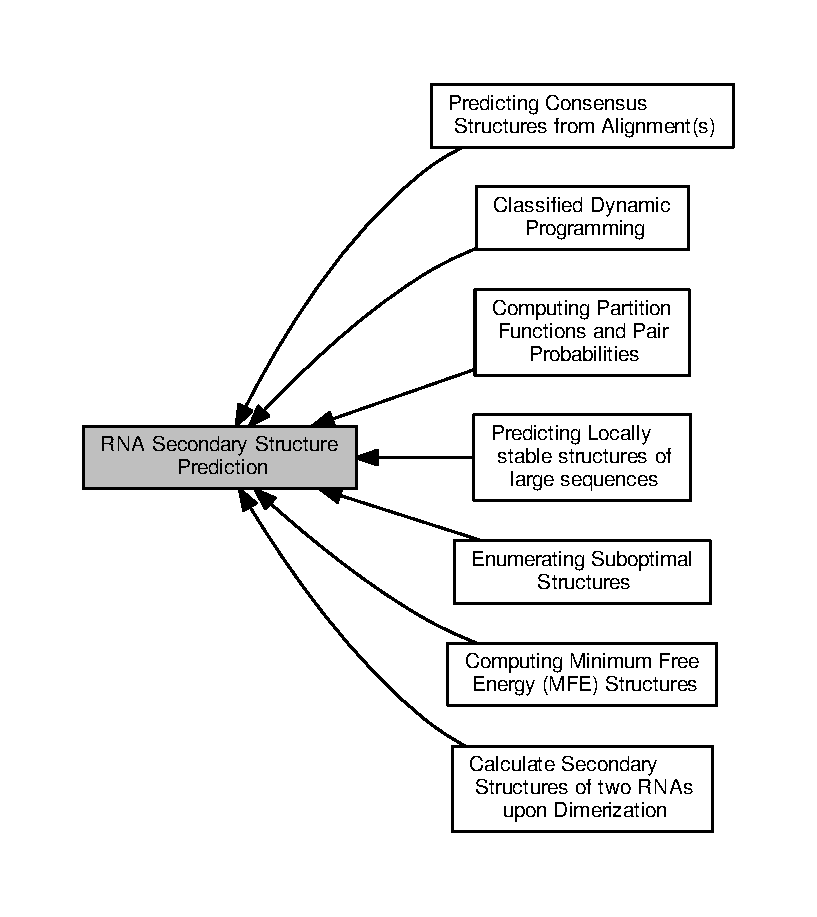
\includegraphics[width=350pt]{group__folding__routines}
\end{center}
\end{figure}
\subsection*{Modules}
\begin{DoxyCompactItemize}
\item 
\hyperlink{group__mfe__fold}{Computing Minimum Free Energy (\+M\+F\+E) Structures}
\begin{DoxyCompactList}\small\item\em This section covers all functions and variables related to the calculation of minimum free energy (M\+F\+E) structures. \end{DoxyCompactList}\item 
\hyperlink{group__pf__fold}{Computing Partition Functions and Pair Probabilities}
\begin{DoxyCompactList}\small\item\em This section provides information about all functions and variables related to the calculation of the partition function and base pair probabilities. \end{DoxyCompactList}\item 
\hyperlink{group__subopt__fold}{Enumerating Suboptimal Structures}
\item 
\hyperlink{group__cofold}{Calculate Secondary Structures of two R\+N\+As upon Dimerization}
\begin{DoxyCompactList}\small\item\em Predict structures formed by two molecules upon hybridization. \end{DoxyCompactList}\item 
\hyperlink{group__consensus__fold}{Predicting Consensus Structures from Alignment(s)}
\begin{DoxyCompactList}\small\item\em compute various properties (consensus M\+F\+E structures, partition function, Boltzmann distributed stochastic samples, ...) for R\+N\+A sequence alignments \end{DoxyCompactList}\item 
\hyperlink{group__local__fold}{Predicting Locally stable structures of large sequences}
\item 
\hyperlink{group__class__fold}{Classified Dynamic Programming}
\end{DoxyCompactItemize}
\subsection*{Files}
\begin{DoxyCompactItemize}
\item 
file \hyperlink{mm_8h}{mm.\+h}
\begin{DoxyCompactList}\small\item\em Several Maximum Matching implementations. \end{DoxyCompactList}\end{DoxyCompactItemize}


\subsection{Detailed Description}
This module contains all functions related to thermodynamic folding of R\+N\+As. 


\hypertarget{group__inverse__fold}{}\section{Inverse Secondary Structure Prediction}
\label{group__inverse__fold}\index{Inverse Secondary Structure Prediction@{Inverse Secondary Structure Prediction}}
\subsection*{Files}
\begin{DoxyCompactItemize}
\item 
file \hyperlink{inverse_8h}{inverse.\+h}
\begin{DoxyCompactList}\small\item\em Inverse folding routines. \end{DoxyCompactList}\end{DoxyCompactItemize}
\subsection*{Functions}
\begin{DoxyCompactItemize}
\item 
float \hyperlink{group__inverse__fold_ga7af026de55d4babad879f2c92559cbbc}{inverse\+\_\+fold} (char $\ast$start, const char $\ast$target)
\begin{DoxyCompactList}\small\item\em Find sequences with predefined structure. \end{DoxyCompactList}\item 
float \hyperlink{group__inverse__fold_gaeef52ecbf2a2450ad585a344f9826806}{inverse\+\_\+pf\+\_\+fold} (char $\ast$start, const char $\ast$target)
\begin{DoxyCompactList}\small\item\em Find sequence that maximizes probability of a predefined structure. \end{DoxyCompactList}\end{DoxyCompactItemize}
\subsection*{Variables}
\begin{DoxyCompactItemize}
\item 
\hypertarget{group__inverse__fold_ga8f791e7740a5a28b9f6fafb4e60301d9}{}char $\ast$ \hyperlink{group__inverse__fold_ga8f791e7740a5a28b9f6fafb4e60301d9}{symbolset}\label{group__inverse__fold_ga8f791e7740a5a28b9f6fafb4e60301d9}

\begin{DoxyCompactList}\small\item\em This global variable points to the allowed bases, initially \char`\"{}\+A\+U\+G\+C\char`\"{}. It can be used to design sequences from reduced alphabets. \end{DoxyCompactList}\item 
float \hyperlink{group__inverse__fold_ga7f17d3b169af048d32bb185039a9c09c}{final\+\_\+cost}
\item 
int \hyperlink{group__inverse__fold_ga7ec4ba51f86e1717a1e174264e4a75ce}{give\+\_\+up}
\item 
int \hyperlink{group__inverse__fold_gafcfc65fba01b9cca5946726ed9057a63}{inv\+\_\+verbose}
\end{DoxyCompactItemize}


\subsection{Detailed Description}
We provide two functions that search for sequences with a given structure, thereby inverting the folding routines. 

\subsection{Function Documentation}
\hypertarget{group__inverse__fold_ga7af026de55d4babad879f2c92559cbbc}{}\index{Inverse Secondary Structure Prediction@{Inverse Secondary Structure Prediction}!inverse\+\_\+fold@{inverse\+\_\+fold}}
\index{inverse\+\_\+fold@{inverse\+\_\+fold}!Inverse Secondary Structure Prediction@{Inverse Secondary Structure Prediction}}
\subsubsection[{inverse\+\_\+fold}]{\setlength{\rightskip}{0pt plus 5cm}float inverse\+\_\+fold (
\begin{DoxyParamCaption}
\item[{char $\ast$}]{start, }
\item[{const char $\ast$}]{target}
\end{DoxyParamCaption}
)}\label{group__inverse__fold_ga7af026de55d4babad879f2c92559cbbc}


{\ttfamily \#include $<$\hyperlink{inverse_8h}{Vienna\+R\+N\+A/inverse.\+h}$>$}



Find sequences with predefined structure. 

This function searches for a sequence with minimum free energy structure provided in the parameter \textquotesingle{}target\textquotesingle{}, starting with sequence \textquotesingle{}start\textquotesingle{}. It returns 0 if the search was successful, otherwise a structure distance in terms of the energy difference between the search result and the actual target \textquotesingle{}target\textquotesingle{} is returned. The found sequence is returned in \textquotesingle{}start\textquotesingle{}. If \hyperlink{group__inverse__fold_ga7ec4ba51f86e1717a1e174264e4a75ce}{give\+\_\+up} is set to 1, the function will return as soon as it is clear that the search will be unsuccessful, this speeds up the algorithm if you are only interested in exact solutions.


\begin{DoxyParams}{Parameters}
{\em start} & The start sequence \\
\hline
{\em target} & The target secondary structure in dot-\/bracket notation \\
\hline
\end{DoxyParams}
\begin{DoxyReturn}{Returns}
The distance to the target in case a search was unsuccessful, 0 otherwise 
\end{DoxyReturn}
\hypertarget{group__inverse__fold_gaeef52ecbf2a2450ad585a344f9826806}{}\index{Inverse Secondary Structure Prediction@{Inverse Secondary Structure Prediction}!inverse\+\_\+pf\+\_\+fold@{inverse\+\_\+pf\+\_\+fold}}
\index{inverse\+\_\+pf\+\_\+fold@{inverse\+\_\+pf\+\_\+fold}!Inverse Secondary Structure Prediction@{Inverse Secondary Structure Prediction}}
\subsubsection[{inverse\+\_\+pf\+\_\+fold}]{\setlength{\rightskip}{0pt plus 5cm}float inverse\+\_\+pf\+\_\+fold (
\begin{DoxyParamCaption}
\item[{char $\ast$}]{start, }
\item[{const char $\ast$}]{target}
\end{DoxyParamCaption}
)}\label{group__inverse__fold_gaeef52ecbf2a2450ad585a344f9826806}


{\ttfamily \#include $<$\hyperlink{inverse_8h}{Vienna\+R\+N\+A/inverse.\+h}$>$}



Find sequence that maximizes probability of a predefined structure. 

This function searches for a sequence with maximum probability to fold into the provided structure \textquotesingle{}target\textquotesingle{} using the partition function algorithm. It returns $-kT \cdot \log(p)$ where $p$ is the frequency of \textquotesingle{}target\textquotesingle{} in the ensemble of possible structures. This is usually much slower than \hyperlink{group__inverse__fold_ga7af026de55d4babad879f2c92559cbbc}{inverse\+\_\+fold()}.


\begin{DoxyParams}{Parameters}
{\em start} & The start sequence \\
\hline
{\em target} & The target secondary structure in dot-\/bracket notation \\
\hline
\end{DoxyParams}
\begin{DoxyReturn}{Returns}
The distance to the target in case a search was unsuccessful, 0 otherwise 
\end{DoxyReturn}


\subsection{Variable Documentation}
\hypertarget{group__inverse__fold_ga7f17d3b169af048d32bb185039a9c09c}{}\index{Inverse Secondary Structure Prediction@{Inverse Secondary Structure Prediction}!final\+\_\+cost@{final\+\_\+cost}}
\index{final\+\_\+cost@{final\+\_\+cost}!Inverse Secondary Structure Prediction@{Inverse Secondary Structure Prediction}}
\subsubsection[{final\+\_\+cost}]{\setlength{\rightskip}{0pt plus 5cm}float final\+\_\+cost}\label{group__inverse__fold_ga7f17d3b169af048d32bb185039a9c09c}


{\ttfamily \#include $<$\hyperlink{inverse_8h}{Vienna\+R\+N\+A/inverse.\+h}$>$}

when to stop \hyperlink{group__inverse__fold_gaeef52ecbf2a2450ad585a344f9826806}{inverse\+\_\+pf\+\_\+fold()} \hypertarget{group__inverse__fold_ga7ec4ba51f86e1717a1e174264e4a75ce}{}\index{Inverse Secondary Structure Prediction@{Inverse Secondary Structure Prediction}!give\+\_\+up@{give\+\_\+up}}
\index{give\+\_\+up@{give\+\_\+up}!Inverse Secondary Structure Prediction@{Inverse Secondary Structure Prediction}}
\subsubsection[{give\+\_\+up}]{\setlength{\rightskip}{0pt plus 5cm}int give\+\_\+up}\label{group__inverse__fold_ga7ec4ba51f86e1717a1e174264e4a75ce}


{\ttfamily \#include $<$\hyperlink{inverse_8h}{Vienna\+R\+N\+A/inverse.\+h}$>$}

default 0\+: try to minimize structure distance even if no exact solution can be found \hypertarget{group__inverse__fold_gafcfc65fba01b9cca5946726ed9057a63}{}\index{Inverse Secondary Structure Prediction@{Inverse Secondary Structure Prediction}!inv\+\_\+verbose@{inv\+\_\+verbose}}
\index{inv\+\_\+verbose@{inv\+\_\+verbose}!Inverse Secondary Structure Prediction@{Inverse Secondary Structure Prediction}}
\subsubsection[{inv\+\_\+verbose}]{\setlength{\rightskip}{0pt plus 5cm}int inv\+\_\+verbose}\label{group__inverse__fold_gafcfc65fba01b9cca5946726ed9057a63}


{\ttfamily \#include $<$\hyperlink{inverse_8h}{Vienna\+R\+N\+A/inverse.\+h}$>$}

print out substructure on which \hyperlink{group__inverse__fold_ga7af026de55d4babad879f2c92559cbbc}{inverse\+\_\+fold()} fails 
\hypertarget{group__paths}{}\section{Refolding paths between secondary structues}
\label{group__paths}\index{Refolding paths between secondary structues@{Refolding paths between secondary structues}}
Collaboration diagram for Refolding paths between secondary structues\+:
\nopagebreak
\begin{figure}[H]
\begin{center}
\leavevmode
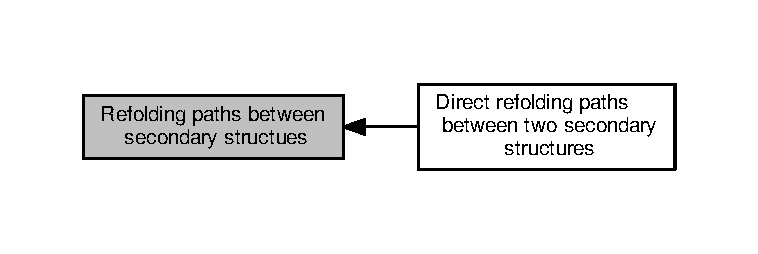
\includegraphics[width=350pt]{group__paths}
\end{center}
\end{figure}
\subsection*{Modules}
\begin{DoxyCompactItemize}
\item 
\hyperlink{group__direct__paths}{Direct refolding paths between two secondary structures}
\begin{DoxyCompactList}\small\item\em Implementation of heuristics to explore optimal (re-\/)folding paths between two secondary structures. \end{DoxyCompactList}\end{DoxyCompactItemize}


\subsection{Detailed Description}

\hypertarget{group__eval}{}\section{Free Energy Evaluation for given Sequence / Structure Pairs}
\label{group__eval}\index{Free Energy Evaluation for given Sequence / Structure Pairs@{Free Energy Evaluation for given Sequence / Structure Pairs}}


This module contains all functions and variables related to energy evaluation of sequence/structure pairs.  


\subsection*{Functions}
\begin{DoxyCompactItemize}
\item 
float \hyperlink{group__eval_ga58f199f1438d794a265f3b27fc8ea631}{vrna\+\_\+eval\+\_\+structure} (\hyperlink{group__fold__compound_ga1b0cef17fd40466cef5968eaeeff6166}{vrna\+\_\+fold\+\_\+compound\+\_\+t} $\ast$vc, const char $\ast$structure)
\begin{DoxyCompactList}\small\item\em Calculate the free energy of an already folded R\+N\+A. \end{DoxyCompactList}\item 
float \hyperlink{group__eval_ga6cea75c0eb9857fb59172be54cab09e0}{vrna\+\_\+eval\+\_\+covar\+\_\+structure} (\hyperlink{group__fold__compound_ga1b0cef17fd40466cef5968eaeeff6166}{vrna\+\_\+fold\+\_\+compound\+\_\+t} $\ast$vc, const char $\ast$structure)
\begin{DoxyCompactList}\small\item\em Calculate the pseudo energy derived by the covariance scores of a set of aligned sequences. \end{DoxyCompactList}\item 
float \hyperlink{group__eval_gab6930f446d04761454d033680fbf7909}{vrna\+\_\+eval\+\_\+structure\+\_\+simple} (const char $\ast$string, const char $\ast$structure)
\begin{DoxyCompactList}\small\item\em Calculate the free energy of an already folded R\+N\+A. \end{DoxyCompactList}\item 
float \hyperlink{group__eval_ga0928d699d310178f84ee2351034e5cb5}{vrna\+\_\+eval\+\_\+structure\+\_\+verbose} (\hyperlink{group__fold__compound_ga1b0cef17fd40466cef5968eaeeff6166}{vrna\+\_\+fold\+\_\+compound\+\_\+t} $\ast$vc, const char $\ast$structure, F\+I\+L\+E $\ast$file)
\begin{DoxyCompactList}\small\item\em Calculate the free energy of an already folded R\+N\+A and print contributions on a per-\/loop base. \end{DoxyCompactList}\item 
float \hyperlink{group__eval_ga4c2895a7dcd756ef2dc7f76db7c4c53e}{vrna\+\_\+eval\+\_\+structure\+\_\+simple\+\_\+verbose} (const char $\ast$string, const char $\ast$structure, F\+I\+L\+E $\ast$file)
\begin{DoxyCompactList}\small\item\em Calculate the free energy of an already folded R\+N\+A and print contributions per loop. \end{DoxyCompactList}\item 
int \hyperlink{group__eval_gadbd09372ddfd7a450bbd590c96a6bfe4}{vrna\+\_\+eval\+\_\+structure\+\_\+pt} (\hyperlink{group__fold__compound_ga1b0cef17fd40466cef5968eaeeff6166}{vrna\+\_\+fold\+\_\+compound\+\_\+t} $\ast$vc, const short $\ast$pt)
\begin{DoxyCompactList}\small\item\em Calculate the free energy of an already folded R\+N\+A. \end{DoxyCompactList}\item 
int \hyperlink{group__eval_ga0bba59b4d6e53461088666ff4aece7b0}{vrna\+\_\+eval\+\_\+structure\+\_\+pt\+\_\+simple} (const char $\ast$string, const short $\ast$pt)
\begin{DoxyCompactList}\small\item\em Calculate the free energy of an already folded R\+N\+A. \end{DoxyCompactList}\item 
int \hyperlink{group__eval_ga8a517cfeeae8c376ae7b1e0c401d38b4}{vrna\+\_\+eval\+\_\+structure\+\_\+pt\+\_\+verbose} (\hyperlink{group__fold__compound_ga1b0cef17fd40466cef5968eaeeff6166}{vrna\+\_\+fold\+\_\+compound\+\_\+t} $\ast$vc, const short $\ast$pt, F\+I\+L\+E $\ast$file)
\begin{DoxyCompactList}\small\item\em Calculate the free energy of an already folded R\+N\+A. \end{DoxyCompactList}\item 
int \hyperlink{group__eval_ga76e152ee9a02be23da14cdddf52b4e44}{vrna\+\_\+eval\+\_\+structure\+\_\+pt\+\_\+simple\+\_\+verbose} (const char $\ast$string, const short $\ast$pt, F\+I\+L\+E $\ast$file)
\begin{DoxyCompactList}\small\item\em Calculate the free energy of an already folded R\+N\+A. \end{DoxyCompactList}\item 
int \hyperlink{group__eval_ga730ba4df55c02fd530a0cddd49faf760}{vrna\+\_\+eval\+\_\+loop\+\_\+pt} (\hyperlink{group__fold__compound_ga1b0cef17fd40466cef5968eaeeff6166}{vrna\+\_\+fold\+\_\+compound\+\_\+t} $\ast$vc, int i, const short $\ast$pt)
\begin{DoxyCompactList}\small\item\em Calculate energy of a loop. \end{DoxyCompactList}\item 
float \hyperlink{group__eval_gaff1b9e4f4d17b434b0a822fe783672c1}{vrna\+\_\+eval\+\_\+move} (\hyperlink{group__fold__compound_ga1b0cef17fd40466cef5968eaeeff6166}{vrna\+\_\+fold\+\_\+compound\+\_\+t} $\ast$vc, const char $\ast$structure, int m1, int m2)
\begin{DoxyCompactList}\small\item\em Calculate energy of a move (closing or opening of a base pair) \end{DoxyCompactList}\item 
int \hyperlink{group__eval_ga123dabc119ea98c968a5e903cc46f0fb}{vrna\+\_\+eval\+\_\+move\+\_\+pt} (\hyperlink{group__fold__compound_ga1b0cef17fd40466cef5968eaeeff6166}{vrna\+\_\+fold\+\_\+compound\+\_\+t} $\ast$vc, short $\ast$pt, int m1, int m2)
\begin{DoxyCompactList}\small\item\em Calculate energy of a move (closing or opening of a base pair) \end{DoxyCompactList}\item 
float \hyperlink{group__eval_gaf93986cb3cb29770ec9cca69c9fab8cf}{energy\+\_\+of\+\_\+structure} (const char $\ast$string, const char $\ast$structure, int verbosity\+\_\+level)
\begin{DoxyCompactList}\small\item\em Calculate the free energy of an already folded R\+N\+A using global model detail settings. \end{DoxyCompactList}\item 
float \hyperlink{group__eval_gaf9d064d3c496de42eca6734a96fd2090}{energy\+\_\+of\+\_\+struct\+\_\+par} (const char $\ast$string, const char $\ast$structure, \hyperlink{group__energy__parameters_ga8a69ca7d787e4fd6079914f5343a1f35}{vrna\+\_\+param\+\_\+t} $\ast$parameters, int verbosity\+\_\+level)
\begin{DoxyCompactList}\small\item\em Calculate the free energy of an already folded R\+N\+A. \end{DoxyCompactList}\item 
float \hyperlink{group__eval_gaeb14f3664aec67fc03268ac75253f0f8}{energy\+\_\+of\+\_\+circ\+\_\+structure} (const char $\ast$string, const char $\ast$structure, int verbosity\+\_\+level)
\begin{DoxyCompactList}\small\item\em Calculate the free energy of an already folded circular R\+N\+A. \end{DoxyCompactList}\item 
float \hyperlink{group__eval_ga3f01f9744ba6a40555eb4d81fc77f6df}{energy\+\_\+of\+\_\+circ\+\_\+struct\+\_\+par} (const char $\ast$string, const char $\ast$structure, \hyperlink{group__energy__parameters_ga8a69ca7d787e4fd6079914f5343a1f35}{vrna\+\_\+param\+\_\+t} $\ast$parameters, int verbosity\+\_\+level)
\begin{DoxyCompactList}\small\item\em Calculate the free energy of an already folded circular R\+N\+A. \end{DoxyCompactList}\item 
int \hyperlink{group__eval_ga8831445966b761417e713360791299d8}{energy\+\_\+of\+\_\+structure\+\_\+pt} (const char $\ast$string, short $\ast$ptable, short $\ast$s, short $\ast$s1, int verbosity\+\_\+level)
\begin{DoxyCompactList}\small\item\em Calculate the free energy of an already folded R\+N\+A. \end{DoxyCompactList}\item 
int \hyperlink{group__eval_ga49acb3d5627dc6823a7ce12d116d4c69}{energy\+\_\+of\+\_\+struct\+\_\+pt\+\_\+par} (const char $\ast$string, short $\ast$ptable, short $\ast$s, short $\ast$s1, \hyperlink{group__energy__parameters_ga8a69ca7d787e4fd6079914f5343a1f35}{vrna\+\_\+param\+\_\+t} $\ast$parameters, int verbosity\+\_\+level)
\begin{DoxyCompactList}\small\item\em Calculate the free energy of an already folded R\+N\+A. \end{DoxyCompactList}\item 
float \hyperlink{group__eval_ga539ecaed89730f7644c202f304d7529b}{energy\+\_\+of\+\_\+move} (const char $\ast$string, const char $\ast$structure, int m1, int m2)
\begin{DoxyCompactList}\small\item\em Calculate energy of a move (closing or opening of a base pair) \end{DoxyCompactList}\item 
int \hyperlink{group__eval_ga49e0ee561be69faf0568213546f6a53f}{energy\+\_\+of\+\_\+move\+\_\+pt} (short $\ast$pt, short $\ast$s, short $\ast$s1, int m1, int m2)
\begin{DoxyCompactList}\small\item\em Calculate energy of a move (closing or opening of a base pair) \end{DoxyCompactList}\item 
int \hyperlink{group__eval_ga507d4fd93f4b398d793ba2402731388d}{loop\+\_\+energy} (short $\ast$ptable, short $\ast$s, short $\ast$s1, int i)
\begin{DoxyCompactList}\small\item\em Calculate energy of a loop. \end{DoxyCompactList}\item 
float \hyperlink{group__eval_gac2b37fea2145c94d925a3f33378ef87b}{energy\+\_\+of\+\_\+struct} (const char $\ast$string, const char $\ast$structure)
\item 
int \hyperlink{group__eval_ga27ce6f68512d43bf1fe14a06c9d76d5c}{energy\+\_\+of\+\_\+struct\+\_\+pt} (const char $\ast$string, short $\ast$ptable, short $\ast$s, short $\ast$s1)
\item 
float \hyperlink{group__eval_ga657222e2758c46bf13b416ef3032e417}{energy\+\_\+of\+\_\+circ\+\_\+struct} (const char $\ast$string, const char $\ast$structure)
\item 
\hypertarget{group__eval_gad3b92453a6b501856eec8fae39f3235d}{}int \hyperlink{group__eval_gad3b92453a6b501856eec8fae39f3235d}{vrna\+\_\+eval\+\_\+ext\+\_\+hp\+\_\+loop} (\hyperlink{group__fold__compound_ga1b0cef17fd40466cef5968eaeeff6166}{vrna\+\_\+fold\+\_\+compound\+\_\+t} $\ast$vc, int i, int j)\label{group__eval_gad3b92453a6b501856eec8fae39f3235d}

\begin{DoxyCompactList}\small\item\em Evaluate free energy of an exterior hairpin loop. \end{DoxyCompactList}\item 
int \hyperlink{group__eval_gab3eb4651dc26dc2b653a57dd340d7e68}{vrna\+\_\+eval\+\_\+hp\+\_\+loop} (\hyperlink{group__fold__compound_ga1b0cef17fd40466cef5968eaeeff6166}{vrna\+\_\+fold\+\_\+compound\+\_\+t} $\ast$vc, int i, int j)
\begin{DoxyCompactList}\small\item\em Evaluate free energy of a hairpin loop. \end{DoxyCompactList}\end{DoxyCompactItemize}
\subsection*{Variables}
\begin{DoxyCompactItemize}
\item 
\hypertarget{group__eval_gab9b2c3a37a5516614c06d0ab54b97cda}{}int \hyperlink{group__eval_gab9b2c3a37a5516614c06d0ab54b97cda}{cut\+\_\+point}\label{group__eval_gab9b2c3a37a5516614c06d0ab54b97cda}

\begin{DoxyCompactList}\small\item\em set to first pos of second seq for cofolding \end{DoxyCompactList}\item 
\hypertarget{group__eval_ga567530678f6260a1a649a5beca5da4c5}{}int \hyperlink{group__eval_ga567530678f6260a1a649a5beca5da4c5}{eos\+\_\+debug}\label{group__eval_ga567530678f6260a1a649a5beca5da4c5}

\begin{DoxyCompactList}\small\item\em verbose info from energy\+\_\+of\+\_\+struct \end{DoxyCompactList}\end{DoxyCompactItemize}


\subsection{Detailed Description}
This module contains all functions and variables related to energy evaluation of sequence/structure pairs. 



\subsection{Function Documentation}
\hypertarget{group__eval_ga58f199f1438d794a265f3b27fc8ea631}{}\index{Free Energy Evaluation for given Sequence / Structure Pairs@{Free Energy Evaluation for given Sequence / Structure Pairs}!vrna\+\_\+eval\+\_\+structure@{vrna\+\_\+eval\+\_\+structure}}
\index{vrna\+\_\+eval\+\_\+structure@{vrna\+\_\+eval\+\_\+structure}!Free Energy Evaluation for given Sequence / Structure Pairs@{Free Energy Evaluation for given Sequence / Structure Pairs}}
\subsubsection[{vrna\+\_\+eval\+\_\+structure}]{\setlength{\rightskip}{0pt plus 5cm}float vrna\+\_\+eval\+\_\+structure (
\begin{DoxyParamCaption}
\item[{{\bf vrna\+\_\+fold\+\_\+compound\+\_\+t} $\ast$}]{vc, }
\item[{const char $\ast$}]{structure}
\end{DoxyParamCaption}
)}\label{group__eval_ga58f199f1438d794a265f3b27fc8ea631}


{\ttfamily \#include $<$\hyperlink{eval_8h}{Vienna\+R\+N\+A/eval.\+h}$>$}



Calculate the free energy of an already folded R\+N\+A. 

This function allows for energy evaluation of a given pair of structure and sequence (alignment). Model details, energy parameters, and possibly soft constraints are used as provided via the parameter \textquotesingle{}vc\textquotesingle{}. The \hyperlink{group__fold__compound_ga1b0cef17fd40466cef5968eaeeff6166}{vrna\+\_\+fold\+\_\+compound\+\_\+t} does not need to contain any D\+P matrices, but requires all most basic init values as one would get from a call like this\+: 
\begin{DoxyCode}
vc = \hyperlink{group__fold__compound_ga6601d994ba32b11511b36f68b08403be}{vrna\_fold\_compound}(sequence, NULL, \hyperlink{group__fold__compound_ga61469c423131552c8483229f8b6c7e0e}{VRNA\_OPTION\_EVAL\_ONLY});
\end{DoxyCode}


\begin{DoxyNote}{Note}
Accepts vrna\+\_\+fold\+\_\+compound\+\_\+t of type \hyperlink{group__fold__compound_gga01a4ff86fa71deaaa5d1abbd95a1447da1608d3aa78905fc39e0d25a624ac9512}{V\+R\+N\+A\+\_\+\+V\+C\+\_\+\+T\+Y\+P\+E\+\_\+\+S\+I\+N\+G\+L\+E} and \hyperlink{group__fold__compound_gga01a4ff86fa71deaaa5d1abbd95a1447da056345f1bcfe7cd595d1fd437c05246d}{V\+R\+N\+A\+\_\+\+V\+C\+\_\+\+T\+Y\+P\+E\+\_\+\+A\+L\+I\+G\+N\+M\+E\+N\+T}
\end{DoxyNote}
\begin{DoxySeeAlso}{See also}
\hyperlink{group__eval_gadbd09372ddfd7a450bbd590c96a6bfe4}{vrna\+\_\+eval\+\_\+structure\+\_\+pt()}, \hyperlink{group__eval_ga0928d699d310178f84ee2351034e5cb5}{vrna\+\_\+eval\+\_\+structure\+\_\+verbose()}, \hyperlink{group__eval_ga8a517cfeeae8c376ae7b1e0c401d38b4}{vrna\+\_\+eval\+\_\+structure\+\_\+pt\+\_\+verbose()}, \hyperlink{group__fold__compound_ga6601d994ba32b11511b36f68b08403be}{vrna\+\_\+fold\+\_\+compound()}, \hyperlink{group__fold__compound_gad6bacc816af274922b13d947f708aa0c}{vrna\+\_\+fold\+\_\+compound\+\_\+comparative()}, \hyperlink{group__eval_ga6cea75c0eb9857fb59172be54cab09e0}{vrna\+\_\+eval\+\_\+covar\+\_\+structure()}
\end{DoxySeeAlso}

\begin{DoxyParams}{Parameters}
{\em vc} & A vrna\+\_\+fold\+\_\+compound\+\_\+t containing the energy parameters and model details \\
\hline
{\em structure} & Secondary structure in dot-\/bracket notation \\
\hline
\end{DoxyParams}
\begin{DoxyReturn}{Returns}
The free energy of the input structure given the input sequence in kcal/mol 
\end{DoxyReturn}
\hypertarget{group__eval_ga6cea75c0eb9857fb59172be54cab09e0}{}\index{Free Energy Evaluation for given Sequence / Structure Pairs@{Free Energy Evaluation for given Sequence / Structure Pairs}!vrna\+\_\+eval\+\_\+covar\+\_\+structure@{vrna\+\_\+eval\+\_\+covar\+\_\+structure}}
\index{vrna\+\_\+eval\+\_\+covar\+\_\+structure@{vrna\+\_\+eval\+\_\+covar\+\_\+structure}!Free Energy Evaluation for given Sequence / Structure Pairs@{Free Energy Evaluation for given Sequence / Structure Pairs}}
\subsubsection[{vrna\+\_\+eval\+\_\+covar\+\_\+structure}]{\setlength{\rightskip}{0pt plus 5cm}float vrna\+\_\+eval\+\_\+covar\+\_\+structure (
\begin{DoxyParamCaption}
\item[{{\bf vrna\+\_\+fold\+\_\+compound\+\_\+t} $\ast$}]{vc, }
\item[{const char $\ast$}]{structure}
\end{DoxyParamCaption}
)}\label{group__eval_ga6cea75c0eb9857fb59172be54cab09e0}


{\ttfamily \#include $<$\hyperlink{eval_8h}{Vienna\+R\+N\+A/eval.\+h}$>$}



Calculate the pseudo energy derived by the covariance scores of a set of aligned sequences. 

Consensus structure prediction is driven by covariance scores of base pairs in rows of the provided alignment. This function allows to retrieve the total amount of this covariance pseudo energy scores. The \hyperlink{group__fold__compound_ga1b0cef17fd40466cef5968eaeeff6166}{vrna\+\_\+fold\+\_\+compound\+\_\+t} does not need to contain any D\+P matrices, but requires all most basic init values as one would get from a call like this\+: 
\begin{DoxyCode}
vc = \hyperlink{group__fold__compound_gad6bacc816af274922b13d947f708aa0c}{vrna\_fold\_compound\_comparative}(alignment, NULL, 
      \hyperlink{group__fold__compound_ga61469c423131552c8483229f8b6c7e0e}{VRNA\_OPTION\_EVAL\_ONLY});
\end{DoxyCode}


\begin{DoxyNote}{Note}
Accepts vrna\+\_\+fold\+\_\+compound\+\_\+t of type \hyperlink{group__fold__compound_gga01a4ff86fa71deaaa5d1abbd95a1447da056345f1bcfe7cd595d1fd437c05246d}{V\+R\+N\+A\+\_\+\+V\+C\+\_\+\+T\+Y\+P\+E\+\_\+\+A\+L\+I\+G\+N\+M\+E\+N\+T} only!
\end{DoxyNote}
\begin{DoxySeeAlso}{See also}
\hyperlink{group__fold__compound_gad6bacc816af274922b13d947f708aa0c}{vrna\+\_\+fold\+\_\+compound\+\_\+comparative()}, \hyperlink{group__eval_ga58f199f1438d794a265f3b27fc8ea631}{vrna\+\_\+eval\+\_\+structure()}
\end{DoxySeeAlso}

\begin{DoxyParams}{Parameters}
{\em vc} & A vrna\+\_\+fold\+\_\+compound\+\_\+t containing the energy parameters and model details \\
\hline
{\em structure} & Secondary (consensus) structure in dot-\/bracket notation \\
\hline
\end{DoxyParams}
\begin{DoxyReturn}{Returns}
The covariance pseudo energy score of the input structure given the input sequence alignment in kcal/mol 
\end{DoxyReturn}
\hypertarget{group__eval_gab6930f446d04761454d033680fbf7909}{}\index{Free Energy Evaluation for given Sequence / Structure Pairs@{Free Energy Evaluation for given Sequence / Structure Pairs}!vrna\+\_\+eval\+\_\+structure\+\_\+simple@{vrna\+\_\+eval\+\_\+structure\+\_\+simple}}
\index{vrna\+\_\+eval\+\_\+structure\+\_\+simple@{vrna\+\_\+eval\+\_\+structure\+\_\+simple}!Free Energy Evaluation for given Sequence / Structure Pairs@{Free Energy Evaluation for given Sequence / Structure Pairs}}
\subsubsection[{vrna\+\_\+eval\+\_\+structure\+\_\+simple}]{\setlength{\rightskip}{0pt plus 5cm}float vrna\+\_\+eval\+\_\+structure\+\_\+simple (
\begin{DoxyParamCaption}
\item[{const char $\ast$}]{string, }
\item[{const char $\ast$}]{structure}
\end{DoxyParamCaption}
)}\label{group__eval_gab6930f446d04761454d033680fbf7909}


{\ttfamily \#include $<$\hyperlink{eval_8h}{Vienna\+R\+N\+A/eval.\+h}$>$}



Calculate the free energy of an already folded R\+N\+A. 

This function allows for energy evaluation of a given sequence/structure pair. In contrast to \hyperlink{group__eval_ga58f199f1438d794a265f3b27fc8ea631}{vrna\+\_\+eval\+\_\+structure()} this function assumes default model details and default energy parameters in order to evaluate the free energy of the secondary structure. Therefore, it serves as a simple interface function for energy evaluation for situations where no changes on the energy model are required.

\begin{DoxySeeAlso}{See also}
\hyperlink{group__eval_ga58f199f1438d794a265f3b27fc8ea631}{vrna\+\_\+eval\+\_\+structure()}, \hyperlink{group__eval_gadbd09372ddfd7a450bbd590c96a6bfe4}{vrna\+\_\+eval\+\_\+structure\+\_\+pt()}, \hyperlink{group__eval_ga0928d699d310178f84ee2351034e5cb5}{vrna\+\_\+eval\+\_\+structure\+\_\+verbose()}, \hyperlink{group__eval_ga8a517cfeeae8c376ae7b1e0c401d38b4}{vrna\+\_\+eval\+\_\+structure\+\_\+pt\+\_\+verbose()},
\end{DoxySeeAlso}

\begin{DoxyParams}{Parameters}
{\em string} & R\+N\+A sequence in uppercase letters \\
\hline
{\em structure} & Secondary structure in dot-\/bracket notation \\
\hline
\end{DoxyParams}
\begin{DoxyReturn}{Returns}
The free energy of the input structure given the input sequence in kcal/mol 
\end{DoxyReturn}
\hypertarget{group__eval_ga0928d699d310178f84ee2351034e5cb5}{}\index{Free Energy Evaluation for given Sequence / Structure Pairs@{Free Energy Evaluation for given Sequence / Structure Pairs}!vrna\+\_\+eval\+\_\+structure\+\_\+verbose@{vrna\+\_\+eval\+\_\+structure\+\_\+verbose}}
\index{vrna\+\_\+eval\+\_\+structure\+\_\+verbose@{vrna\+\_\+eval\+\_\+structure\+\_\+verbose}!Free Energy Evaluation for given Sequence / Structure Pairs@{Free Energy Evaluation for given Sequence / Structure Pairs}}
\subsubsection[{vrna\+\_\+eval\+\_\+structure\+\_\+verbose}]{\setlength{\rightskip}{0pt plus 5cm}float vrna\+\_\+eval\+\_\+structure\+\_\+verbose (
\begin{DoxyParamCaption}
\item[{{\bf vrna\+\_\+fold\+\_\+compound\+\_\+t} $\ast$}]{vc, }
\item[{const char $\ast$}]{structure, }
\item[{F\+I\+L\+E $\ast$}]{file}
\end{DoxyParamCaption}
)}\label{group__eval_ga0928d699d310178f84ee2351034e5cb5}


{\ttfamily \#include $<$\hyperlink{eval_8h}{Vienna\+R\+N\+A/eval.\+h}$>$}



Calculate the free energy of an already folded R\+N\+A and print contributions on a per-\/loop base. 

This function allows for detailed energy evaluation of a given sequence/structure pair. In contrast to \hyperlink{group__eval_ga58f199f1438d794a265f3b27fc8ea631}{vrna\+\_\+eval\+\_\+structure()} this function prints detailed energy contributions based on individual loops to a file handle. If N\+U\+L\+L is passed as file handle, this function defaults to print to stdout. Model details, energy parameters, and possibly soft constraints are used as provided via the parameter \textquotesingle{}vc\textquotesingle{}. The fold\+\_\+compound does not need to contain any D\+P matrices, but all the most basic init values as one would get from a call like this\+: 
\begin{DoxyCode}
vc = \hyperlink{group__fold__compound_ga6601d994ba32b11511b36f68b08403be}{vrna\_fold\_compound}(sequence, NULL, \hyperlink{group__fold__compound_ga61469c423131552c8483229f8b6c7e0e}{VRNA\_OPTION\_EVAL\_ONLY});
\end{DoxyCode}


\begin{DoxySeeAlso}{See also}
\hyperlink{group__eval_gadbd09372ddfd7a450bbd590c96a6bfe4}{vrna\+\_\+eval\+\_\+structure\+\_\+pt()}, \hyperlink{group__eval_ga0928d699d310178f84ee2351034e5cb5}{vrna\+\_\+eval\+\_\+structure\+\_\+verbose()}, \hyperlink{group__eval_ga8a517cfeeae8c376ae7b1e0c401d38b4}{vrna\+\_\+eval\+\_\+structure\+\_\+pt\+\_\+verbose()},
\end{DoxySeeAlso}

\begin{DoxyParams}{Parameters}
{\em vc} & A vrna\+\_\+fold\+\_\+compound\+\_\+t containing the energy parameters and model details \\
\hline
{\em structure} & Secondary structure in dot-\/bracket notation \\
\hline
{\em file} & A file handle where this function should print to (may be N\+U\+L\+L). \\
\hline
\end{DoxyParams}
\begin{DoxyReturn}{Returns}
The free energy of the input structure given the input sequence in kcal/mol 
\end{DoxyReturn}
\hypertarget{group__eval_ga4c2895a7dcd756ef2dc7f76db7c4c53e}{}\index{Free Energy Evaluation for given Sequence / Structure Pairs@{Free Energy Evaluation for given Sequence / Structure Pairs}!vrna\+\_\+eval\+\_\+structure\+\_\+simple\+\_\+verbose@{vrna\+\_\+eval\+\_\+structure\+\_\+simple\+\_\+verbose}}
\index{vrna\+\_\+eval\+\_\+structure\+\_\+simple\+\_\+verbose@{vrna\+\_\+eval\+\_\+structure\+\_\+simple\+\_\+verbose}!Free Energy Evaluation for given Sequence / Structure Pairs@{Free Energy Evaluation for given Sequence / Structure Pairs}}
\subsubsection[{vrna\+\_\+eval\+\_\+structure\+\_\+simple\+\_\+verbose}]{\setlength{\rightskip}{0pt plus 5cm}float vrna\+\_\+eval\+\_\+structure\+\_\+simple\+\_\+verbose (
\begin{DoxyParamCaption}
\item[{const char $\ast$}]{string, }
\item[{const char $\ast$}]{structure, }
\item[{F\+I\+L\+E $\ast$}]{file}
\end{DoxyParamCaption}
)}\label{group__eval_ga4c2895a7dcd756ef2dc7f76db7c4c53e}


{\ttfamily \#include $<$\hyperlink{eval_8h}{Vienna\+R\+N\+A/eval.\+h}$>$}



Calculate the free energy of an already folded R\+N\+A and print contributions per loop. 

This function allows for detailed energy evaluation of a given sequence/structure pair. In contrast to \hyperlink{group__eval_ga58f199f1438d794a265f3b27fc8ea631}{vrna\+\_\+eval\+\_\+structure()} this function prints detailed energy contributions based on individual loops to a file handle. If N\+U\+L\+L is passed as file handle, this function defaults to print to stdout. In contrast to \hyperlink{group__eval_ga0928d699d310178f84ee2351034e5cb5}{vrna\+\_\+eval\+\_\+structure\+\_\+verbose()} this function assumes default model details and default energy parameters in order to evaluate the free energy of the secondary structure. Threefore, it serves as a simple interface function for energy evaluation for situations where no changes on the energy model are required.

\begin{DoxySeeAlso}{See also}
\hyperlink{group__eval_ga0928d699d310178f84ee2351034e5cb5}{vrna\+\_\+eval\+\_\+structure\+\_\+verbose()}, \hyperlink{group__eval_gadbd09372ddfd7a450bbd590c96a6bfe4}{vrna\+\_\+eval\+\_\+structure\+\_\+pt()}, \hyperlink{group__eval_ga0928d699d310178f84ee2351034e5cb5}{vrna\+\_\+eval\+\_\+structure\+\_\+verbose()}, \hyperlink{group__eval_ga8a517cfeeae8c376ae7b1e0c401d38b4}{vrna\+\_\+eval\+\_\+structure\+\_\+pt\+\_\+verbose()},
\end{DoxySeeAlso}

\begin{DoxyParams}{Parameters}
{\em string} & R\+N\+A sequence in uppercase letters \\
\hline
{\em structure} & Secondary structure in dot-\/bracket notation \\
\hline
{\em file} & A file handle where this function should print to (may be N\+U\+L\+L). \\
\hline
\end{DoxyParams}
\begin{DoxyReturn}{Returns}
The free energy of the input structure given the input sequence in kcal/mol 
\end{DoxyReturn}
\hypertarget{group__eval_gadbd09372ddfd7a450bbd590c96a6bfe4}{}\index{Free Energy Evaluation for given Sequence / Structure Pairs@{Free Energy Evaluation for given Sequence / Structure Pairs}!vrna\+\_\+eval\+\_\+structure\+\_\+pt@{vrna\+\_\+eval\+\_\+structure\+\_\+pt}}
\index{vrna\+\_\+eval\+\_\+structure\+\_\+pt@{vrna\+\_\+eval\+\_\+structure\+\_\+pt}!Free Energy Evaluation for given Sequence / Structure Pairs@{Free Energy Evaluation for given Sequence / Structure Pairs}}
\subsubsection[{vrna\+\_\+eval\+\_\+structure\+\_\+pt}]{\setlength{\rightskip}{0pt plus 5cm}int vrna\+\_\+eval\+\_\+structure\+\_\+pt (
\begin{DoxyParamCaption}
\item[{{\bf vrna\+\_\+fold\+\_\+compound\+\_\+t} $\ast$}]{vc, }
\item[{const short $\ast$}]{pt}
\end{DoxyParamCaption}
)}\label{group__eval_gadbd09372ddfd7a450bbd590c96a6bfe4}


{\ttfamily \#include $<$\hyperlink{eval_8h}{Vienna\+R\+N\+A/eval.\+h}$>$}



Calculate the free energy of an already folded R\+N\+A. 

This function allows for energy evaluation of a given sequence/structure pair where the structure is provided in pair\+\_\+table format as obtained from \hyperlink{group__struct__utils_gae829fb8bb7f694c12a9c0bbc34c77c60}{vrna\+\_\+ptable()}. Model details, energy parameters, and possibly soft constraints are used as provided via the parameter \textquotesingle{}vc\textquotesingle{}. The fold\+\_\+compound does not need to contain any D\+P matrices, but all the most basic init values as one would get from a call like this\+: 
\begin{DoxyCode}
vc = \hyperlink{group__fold__compound_ga6601d994ba32b11511b36f68b08403be}{vrna\_fold\_compound}(sequence, NULL, \hyperlink{group__fold__compound_ga61469c423131552c8483229f8b6c7e0e}{VRNA\_OPTION\_EVAL\_ONLY});
\end{DoxyCode}


\begin{DoxySeeAlso}{See also}
\hyperlink{group__struct__utils_gae829fb8bb7f694c12a9c0bbc34c77c60}{vrna\+\_\+ptable()}, \hyperlink{group__eval_ga58f199f1438d794a265f3b27fc8ea631}{vrna\+\_\+eval\+\_\+structure()}, \hyperlink{group__eval_ga8a517cfeeae8c376ae7b1e0c401d38b4}{vrna\+\_\+eval\+\_\+structure\+\_\+pt\+\_\+verbose()}
\end{DoxySeeAlso}

\begin{DoxyParams}{Parameters}
{\em vc} & A vrna\+\_\+fold\+\_\+compound\+\_\+t containing the energy parameters and model details \\
\hline
{\em pt} & Secondary structure as pair\+\_\+table \\
\hline
\end{DoxyParams}
\begin{DoxyReturn}{Returns}
The free energy of the input structure given the input sequence in 10cal/mol 
\end{DoxyReturn}
\hypertarget{group__eval_ga0bba59b4d6e53461088666ff4aece7b0}{}\index{Free Energy Evaluation for given Sequence / Structure Pairs@{Free Energy Evaluation for given Sequence / Structure Pairs}!vrna\+\_\+eval\+\_\+structure\+\_\+pt\+\_\+simple@{vrna\+\_\+eval\+\_\+structure\+\_\+pt\+\_\+simple}}
\index{vrna\+\_\+eval\+\_\+structure\+\_\+pt\+\_\+simple@{vrna\+\_\+eval\+\_\+structure\+\_\+pt\+\_\+simple}!Free Energy Evaluation for given Sequence / Structure Pairs@{Free Energy Evaluation for given Sequence / Structure Pairs}}
\subsubsection[{vrna\+\_\+eval\+\_\+structure\+\_\+pt\+\_\+simple}]{\setlength{\rightskip}{0pt plus 5cm}int vrna\+\_\+eval\+\_\+structure\+\_\+pt\+\_\+simple (
\begin{DoxyParamCaption}
\item[{const char $\ast$}]{string, }
\item[{const short $\ast$}]{pt}
\end{DoxyParamCaption}
)}\label{group__eval_ga0bba59b4d6e53461088666ff4aece7b0}


{\ttfamily \#include $<$\hyperlink{eval_8h}{Vienna\+R\+N\+A/eval.\+h}$>$}



Calculate the free energy of an already folded R\+N\+A. 

In contrast to \hyperlink{group__eval_gadbd09372ddfd7a450bbd590c96a6bfe4}{vrna\+\_\+eval\+\_\+structure\+\_\+pt()} this function assumes default model details and default energy parameters in order to evaluate the free energy of the secondary structure. Threefore, it serves as a simple interface function for energy evaluation for situations where no changes on the energy model are required.

\begin{DoxySeeAlso}{See also}
\hyperlink{group__struct__utils_gae829fb8bb7f694c12a9c0bbc34c77c60}{vrna\+\_\+ptable()}, \hyperlink{group__eval_gab6930f446d04761454d033680fbf7909}{vrna\+\_\+eval\+\_\+structure\+\_\+simple()}, \hyperlink{group__eval_gadbd09372ddfd7a450bbd590c96a6bfe4}{vrna\+\_\+eval\+\_\+structure\+\_\+pt()}
\end{DoxySeeAlso}

\begin{DoxyParams}{Parameters}
{\em string} & R\+N\+A sequence in uppercase letters \\
\hline
{\em pt} & Secondary structure as pair\+\_\+table \\
\hline
\end{DoxyParams}
\begin{DoxyReturn}{Returns}
The free energy of the input structure given the input sequence in 10cal/mol 
\end{DoxyReturn}
\hypertarget{group__eval_ga8a517cfeeae8c376ae7b1e0c401d38b4}{}\index{Free Energy Evaluation for given Sequence / Structure Pairs@{Free Energy Evaluation for given Sequence / Structure Pairs}!vrna\+\_\+eval\+\_\+structure\+\_\+pt\+\_\+verbose@{vrna\+\_\+eval\+\_\+structure\+\_\+pt\+\_\+verbose}}
\index{vrna\+\_\+eval\+\_\+structure\+\_\+pt\+\_\+verbose@{vrna\+\_\+eval\+\_\+structure\+\_\+pt\+\_\+verbose}!Free Energy Evaluation for given Sequence / Structure Pairs@{Free Energy Evaluation for given Sequence / Structure Pairs}}
\subsubsection[{vrna\+\_\+eval\+\_\+structure\+\_\+pt\+\_\+verbose}]{\setlength{\rightskip}{0pt plus 5cm}int vrna\+\_\+eval\+\_\+structure\+\_\+pt\+\_\+verbose (
\begin{DoxyParamCaption}
\item[{{\bf vrna\+\_\+fold\+\_\+compound\+\_\+t} $\ast$}]{vc, }
\item[{const short $\ast$}]{pt, }
\item[{F\+I\+L\+E $\ast$}]{file}
\end{DoxyParamCaption}
)}\label{group__eval_ga8a517cfeeae8c376ae7b1e0c401d38b4}


{\ttfamily \#include $<$\hyperlink{eval_8h}{Vienna\+R\+N\+A/eval.\+h}$>$}



Calculate the free energy of an already folded R\+N\+A. 

This function allows for energy evaluation of a given sequence/structure pair where the structure is provided in pair\+\_\+table format as obtained from \hyperlink{group__struct__utils_gae829fb8bb7f694c12a9c0bbc34c77c60}{vrna\+\_\+ptable()}. Model details, energy parameters, and possibly soft constraints are used as provided via the parameter \textquotesingle{}vc\textquotesingle{}. The fold\+\_\+compound does not need to contain any D\+P matrices, but all the most basic init values as one would get from a call like this\+: 
\begin{DoxyCode}
vc = \hyperlink{group__fold__compound_ga6601d994ba32b11511b36f68b08403be}{vrna\_fold\_compound}(sequence, NULL, \hyperlink{group__fold__compound_ga61469c423131552c8483229f8b6c7e0e}{VRNA\_OPTION\_EVAL\_ONLY});
\end{DoxyCode}
 In contrast to \hyperlink{group__eval_gadbd09372ddfd7a450bbd590c96a6bfe4}{vrna\+\_\+eval\+\_\+structure\+\_\+pt()} this function prints detailed energy contributions based on individual loops to a file handle. If N\+U\+L\+L is passed as file handle, this function defaults to print to stdout.

\begin{DoxySeeAlso}{See also}
\hyperlink{group__struct__utils_gae829fb8bb7f694c12a9c0bbc34c77c60}{vrna\+\_\+ptable()}, \hyperlink{group__eval_gadbd09372ddfd7a450bbd590c96a6bfe4}{vrna\+\_\+eval\+\_\+structure\+\_\+pt()}, \hyperlink{group__eval_ga0928d699d310178f84ee2351034e5cb5}{vrna\+\_\+eval\+\_\+structure\+\_\+verbose()}
\end{DoxySeeAlso}

\begin{DoxyParams}{Parameters}
{\em vc} & A vrna\+\_\+fold\+\_\+compound\+\_\+t containing the energy parameters and model details \\
\hline
{\em pt} & Secondary structure as pair\+\_\+table \\
\hline
{\em file} & A file handle where this function should print to (may be N\+U\+L\+L). \\
\hline
\end{DoxyParams}
\begin{DoxyReturn}{Returns}
The free energy of the input structure given the input sequence in 10cal/mol 
\end{DoxyReturn}
\hypertarget{group__eval_ga76e152ee9a02be23da14cdddf52b4e44}{}\index{Free Energy Evaluation for given Sequence / Structure Pairs@{Free Energy Evaluation for given Sequence / Structure Pairs}!vrna\+\_\+eval\+\_\+structure\+\_\+pt\+\_\+simple\+\_\+verbose@{vrna\+\_\+eval\+\_\+structure\+\_\+pt\+\_\+simple\+\_\+verbose}}
\index{vrna\+\_\+eval\+\_\+structure\+\_\+pt\+\_\+simple\+\_\+verbose@{vrna\+\_\+eval\+\_\+structure\+\_\+pt\+\_\+simple\+\_\+verbose}!Free Energy Evaluation for given Sequence / Structure Pairs@{Free Energy Evaluation for given Sequence / Structure Pairs}}
\subsubsection[{vrna\+\_\+eval\+\_\+structure\+\_\+pt\+\_\+simple\+\_\+verbose}]{\setlength{\rightskip}{0pt plus 5cm}int vrna\+\_\+eval\+\_\+structure\+\_\+pt\+\_\+simple\+\_\+verbose (
\begin{DoxyParamCaption}
\item[{const char $\ast$}]{string, }
\item[{const short $\ast$}]{pt, }
\item[{F\+I\+L\+E $\ast$}]{file}
\end{DoxyParamCaption}
)}\label{group__eval_ga76e152ee9a02be23da14cdddf52b4e44}


{\ttfamily \#include $<$\hyperlink{eval_8h}{Vienna\+R\+N\+A/eval.\+h}$>$}



Calculate the free energy of an already folded R\+N\+A. 

This function allows for energy evaluation of a given sequence/structure pair where the structure is provided in pair\+\_\+table format as obtained from \hyperlink{group__struct__utils_gae829fb8bb7f694c12a9c0bbc34c77c60}{vrna\+\_\+ptable()}. Model details, energy parameters, and possibly soft constraints are used as provided via the parameter \textquotesingle{}vc\textquotesingle{}. The fold\+\_\+compound does not need to contain any D\+P matrices, but all the most basic init values as one would get from a call like this\+: 
\begin{DoxyCode}
vc = \hyperlink{group__fold__compound_ga6601d994ba32b11511b36f68b08403be}{vrna\_fold\_compound}(sequence, NULL, \hyperlink{group__fold__compound_ga61469c423131552c8483229f8b6c7e0e}{VRNA\_OPTION\_EVAL\_ONLY});
\end{DoxyCode}
 In contrast to \hyperlink{group__eval_ga8a517cfeeae8c376ae7b1e0c401d38b4}{vrna\+\_\+eval\+\_\+structure\+\_\+pt\+\_\+verbose()} this function assumes default model details and default energy parameters in order to evaluate the free energy of the secondary structure. Threefore, it serves as a simple interface function for energy evaluation for situations where no changes on the energy model are required.

\begin{DoxySeeAlso}{See also}
\hyperlink{group__struct__utils_gae829fb8bb7f694c12a9c0bbc34c77c60}{vrna\+\_\+ptable()}, \hyperlink{group__eval_ga8a517cfeeae8c376ae7b1e0c401d38b4}{vrna\+\_\+eval\+\_\+structure\+\_\+pt\+\_\+verbose()}, \hyperlink{group__eval_gab6930f446d04761454d033680fbf7909}{vrna\+\_\+eval\+\_\+structure\+\_\+simple()}
\end{DoxySeeAlso}

\begin{DoxyParams}{Parameters}
{\em string} & R\+N\+A sequence in uppercase letters \\
\hline
{\em pt} & Secondary structure as pair\+\_\+table \\
\hline
{\em file} & A file handle where this function should print to (may be N\+U\+L\+L). \\
\hline
\end{DoxyParams}
\begin{DoxyReturn}{Returns}
The free energy of the input structure given the input sequence in 10cal/mol 
\end{DoxyReturn}
\hypertarget{group__eval_ga730ba4df55c02fd530a0cddd49faf760}{}\index{Free Energy Evaluation for given Sequence / Structure Pairs@{Free Energy Evaluation for given Sequence / Structure Pairs}!vrna\+\_\+eval\+\_\+loop\+\_\+pt@{vrna\+\_\+eval\+\_\+loop\+\_\+pt}}
\index{vrna\+\_\+eval\+\_\+loop\+\_\+pt@{vrna\+\_\+eval\+\_\+loop\+\_\+pt}!Free Energy Evaluation for given Sequence / Structure Pairs@{Free Energy Evaluation for given Sequence / Structure Pairs}}
\subsubsection[{vrna\+\_\+eval\+\_\+loop\+\_\+pt}]{\setlength{\rightskip}{0pt plus 5cm}int vrna\+\_\+eval\+\_\+loop\+\_\+pt (
\begin{DoxyParamCaption}
\item[{{\bf vrna\+\_\+fold\+\_\+compound\+\_\+t} $\ast$}]{vc, }
\item[{int}]{i, }
\item[{const short $\ast$}]{pt}
\end{DoxyParamCaption}
)}\label{group__eval_ga730ba4df55c02fd530a0cddd49faf760}


{\ttfamily \#include $<$\hyperlink{eval_8h}{Vienna\+R\+N\+A/eval.\+h}$>$}



Calculate energy of a loop. 


\begin{DoxyParams}{Parameters}
{\em vc} & A vrna\+\_\+fold\+\_\+compound\+\_\+t containing the energy parameters and model details \\
\hline
{\em i} & position of covering base pair \\
\hline
{\em pt} & the pair table of the secondary structure \\
\hline
\end{DoxyParams}
\begin{DoxyReturn}{Returns}
free energy of the loop in 10cal/mol 
\end{DoxyReturn}
\hypertarget{group__eval_gaff1b9e4f4d17b434b0a822fe783672c1}{}\index{Free Energy Evaluation for given Sequence / Structure Pairs@{Free Energy Evaluation for given Sequence / Structure Pairs}!vrna\+\_\+eval\+\_\+move@{vrna\+\_\+eval\+\_\+move}}
\index{vrna\+\_\+eval\+\_\+move@{vrna\+\_\+eval\+\_\+move}!Free Energy Evaluation for given Sequence / Structure Pairs@{Free Energy Evaluation for given Sequence / Structure Pairs}}
\subsubsection[{vrna\+\_\+eval\+\_\+move}]{\setlength{\rightskip}{0pt plus 5cm}float vrna\+\_\+eval\+\_\+move (
\begin{DoxyParamCaption}
\item[{{\bf vrna\+\_\+fold\+\_\+compound\+\_\+t} $\ast$}]{vc, }
\item[{const char $\ast$}]{structure, }
\item[{int}]{m1, }
\item[{int}]{m2}
\end{DoxyParamCaption}
)}\label{group__eval_gaff1b9e4f4d17b434b0a822fe783672c1}


{\ttfamily \#include $<$\hyperlink{eval_8h}{Vienna\+R\+N\+A/eval.\+h}$>$}



Calculate energy of a move (closing or opening of a base pair) 

If the parameters m1 and m2 are negative, it is deletion (opening) of a base pair, otherwise it is insertion (opening).

\begin{DoxySeeAlso}{See also}
\hyperlink{group__eval_ga123dabc119ea98c968a5e903cc46f0fb}{vrna\+\_\+eval\+\_\+move\+\_\+pt()} 
\end{DoxySeeAlso}

\begin{DoxyParams}{Parameters}
{\em vc} & A vrna\+\_\+fold\+\_\+compound\+\_\+t containing the energy parameters and model details \\
\hline
{\em structure} & secondary structure in dot-\/bracket notation \\
\hline
{\em m1} & first coordinate of base pair \\
\hline
{\em m2} & second coordinate of base pair \\
\hline
\end{DoxyParams}
\begin{DoxyReturn}{Returns}
energy change of the move in kcal/mol 
\end{DoxyReturn}
\hypertarget{group__eval_ga123dabc119ea98c968a5e903cc46f0fb}{}\index{Free Energy Evaluation for given Sequence / Structure Pairs@{Free Energy Evaluation for given Sequence / Structure Pairs}!vrna\+\_\+eval\+\_\+move\+\_\+pt@{vrna\+\_\+eval\+\_\+move\+\_\+pt}}
\index{vrna\+\_\+eval\+\_\+move\+\_\+pt@{vrna\+\_\+eval\+\_\+move\+\_\+pt}!Free Energy Evaluation for given Sequence / Structure Pairs@{Free Energy Evaluation for given Sequence / Structure Pairs}}
\subsubsection[{vrna\+\_\+eval\+\_\+move\+\_\+pt}]{\setlength{\rightskip}{0pt plus 5cm}int vrna\+\_\+eval\+\_\+move\+\_\+pt (
\begin{DoxyParamCaption}
\item[{{\bf vrna\+\_\+fold\+\_\+compound\+\_\+t} $\ast$}]{vc, }
\item[{short $\ast$}]{pt, }
\item[{int}]{m1, }
\item[{int}]{m2}
\end{DoxyParamCaption}
)}\label{group__eval_ga123dabc119ea98c968a5e903cc46f0fb}


{\ttfamily \#include $<$\hyperlink{eval_8h}{Vienna\+R\+N\+A/eval.\+h}$>$}



Calculate energy of a move (closing or opening of a base pair) 

If the parameters m1 and m2 are negative, it is deletion (opening) of a base pair, otherwise it is insertion (opening).

\begin{DoxySeeAlso}{See also}
\hyperlink{group__eval_gaff1b9e4f4d17b434b0a822fe783672c1}{vrna\+\_\+eval\+\_\+move()} 
\end{DoxySeeAlso}

\begin{DoxyParams}{Parameters}
{\em vc} & A vrna\+\_\+fold\+\_\+compound\+\_\+t containing the energy parameters and model details \\
\hline
{\em pt} & the pair table of the secondary structure \\
\hline
{\em m1} & first coordinate of base pair \\
\hline
{\em m2} & second coordinate of base pair \\
\hline
\end{DoxyParams}
\begin{DoxyReturn}{Returns}
energy change of the move in 10cal/mol 
\end{DoxyReturn}
\hypertarget{group__eval_gaf93986cb3cb29770ec9cca69c9fab8cf}{}\index{Free Energy Evaluation for given Sequence / Structure Pairs@{Free Energy Evaluation for given Sequence / Structure Pairs}!energy\+\_\+of\+\_\+structure@{energy\+\_\+of\+\_\+structure}}
\index{energy\+\_\+of\+\_\+structure@{energy\+\_\+of\+\_\+structure}!Free Energy Evaluation for given Sequence / Structure Pairs@{Free Energy Evaluation for given Sequence / Structure Pairs}}
\subsubsection[{energy\+\_\+of\+\_\+structure}]{\setlength{\rightskip}{0pt plus 5cm}float energy\+\_\+of\+\_\+structure (
\begin{DoxyParamCaption}
\item[{const char $\ast$}]{string, }
\item[{const char $\ast$}]{structure, }
\item[{int}]{verbosity\+\_\+level}
\end{DoxyParamCaption}
)}\label{group__eval_gaf93986cb3cb29770ec9cca69c9fab8cf}


{\ttfamily \#include $<$\hyperlink{eval_8h}{Vienna\+R\+N\+A/eval.\+h}$>$}



Calculate the free energy of an already folded R\+N\+A using global model detail settings. 

If verbosity level is set to a value $>$0, energies of structure elements are printed to stdout

\begin{DoxyNote}{Note}
Open\+M\+P\+: This function relies on several global model settings variables and thus is not to be considered threadsafe. See \hyperlink{group__eval_gaf9d064d3c496de42eca6734a96fd2090}{energy\+\_\+of\+\_\+struct\+\_\+par()} for a completely threadsafe implementation.
\end{DoxyNote}
\begin{DoxyRefDesc}{Deprecated}
\item[\hyperlink{deprecated__deprecated000053}{Deprecated}]Use \hyperlink{group__eval_ga58f199f1438d794a265f3b27fc8ea631}{vrna\+\_\+eval\+\_\+structure()} or \hyperlink{group__eval_ga0928d699d310178f84ee2351034e5cb5}{vrna\+\_\+eval\+\_\+structure\+\_\+verbose()} instead!\end{DoxyRefDesc}


\begin{DoxySeeAlso}{See also}
\hyperlink{group__eval_ga58f199f1438d794a265f3b27fc8ea631}{vrna\+\_\+eval\+\_\+structure()}
\end{DoxySeeAlso}

\begin{DoxyParams}{Parameters}
{\em string} & R\+N\+A sequence \\
\hline
{\em structure} & secondary structure in dot-\/bracket notation \\
\hline
{\em verbosity\+\_\+level} & a flag to turn verbose output on/off \\
\hline
\end{DoxyParams}
\begin{DoxyReturn}{Returns}
the free energy of the input structure given the input sequence in kcal/mol 
\end{DoxyReturn}
\hypertarget{group__eval_gaf9d064d3c496de42eca6734a96fd2090}{}\index{Free Energy Evaluation for given Sequence / Structure Pairs@{Free Energy Evaluation for given Sequence / Structure Pairs}!energy\+\_\+of\+\_\+struct\+\_\+par@{energy\+\_\+of\+\_\+struct\+\_\+par}}
\index{energy\+\_\+of\+\_\+struct\+\_\+par@{energy\+\_\+of\+\_\+struct\+\_\+par}!Free Energy Evaluation for given Sequence / Structure Pairs@{Free Energy Evaluation for given Sequence / Structure Pairs}}
\subsubsection[{energy\+\_\+of\+\_\+struct\+\_\+par}]{\setlength{\rightskip}{0pt plus 5cm}float energy\+\_\+of\+\_\+struct\+\_\+par (
\begin{DoxyParamCaption}
\item[{const char $\ast$}]{string, }
\item[{const char $\ast$}]{structure, }
\item[{{\bf vrna\+\_\+param\+\_\+t} $\ast$}]{parameters, }
\item[{int}]{verbosity\+\_\+level}
\end{DoxyParamCaption}
)}\label{group__eval_gaf9d064d3c496de42eca6734a96fd2090}


{\ttfamily \#include $<$\hyperlink{eval_8h}{Vienna\+R\+N\+A/eval.\+h}$>$}



Calculate the free energy of an already folded R\+N\+A. 

If verbosity level is set to a value $>$0, energies of structure elements are printed to stdout

\begin{DoxyRefDesc}{Deprecated}
\item[\hyperlink{deprecated__deprecated000054}{Deprecated}]Use \hyperlink{group__eval_ga58f199f1438d794a265f3b27fc8ea631}{vrna\+\_\+eval\+\_\+structure()} or \hyperlink{group__eval_ga0928d699d310178f84ee2351034e5cb5}{vrna\+\_\+eval\+\_\+structure\+\_\+verbose()} instead!\end{DoxyRefDesc}


\begin{DoxySeeAlso}{See also}
\hyperlink{group__eval_ga58f199f1438d794a265f3b27fc8ea631}{vrna\+\_\+eval\+\_\+structure()}
\end{DoxySeeAlso}

\begin{DoxyParams}{Parameters}
{\em string} & R\+N\+A sequence in uppercase letters \\
\hline
{\em structure} & Secondary structure in dot-\/bracket notation \\
\hline
{\em parameters} & A data structure containing the prescaled energy contributions and the model details. \\
\hline
{\em verbosity\+\_\+level} & A flag to turn verbose output on/off \\
\hline
\end{DoxyParams}
\begin{DoxyReturn}{Returns}
The free energy of the input structure given the input sequence in kcal/mol 
\end{DoxyReturn}
\hypertarget{group__eval_gaeb14f3664aec67fc03268ac75253f0f8}{}\index{Free Energy Evaluation for given Sequence / Structure Pairs@{Free Energy Evaluation for given Sequence / Structure Pairs}!energy\+\_\+of\+\_\+circ\+\_\+structure@{energy\+\_\+of\+\_\+circ\+\_\+structure}}
\index{energy\+\_\+of\+\_\+circ\+\_\+structure@{energy\+\_\+of\+\_\+circ\+\_\+structure}!Free Energy Evaluation for given Sequence / Structure Pairs@{Free Energy Evaluation for given Sequence / Structure Pairs}}
\subsubsection[{energy\+\_\+of\+\_\+circ\+\_\+structure}]{\setlength{\rightskip}{0pt plus 5cm}float energy\+\_\+of\+\_\+circ\+\_\+structure (
\begin{DoxyParamCaption}
\item[{const char $\ast$}]{string, }
\item[{const char $\ast$}]{structure, }
\item[{int}]{verbosity\+\_\+level}
\end{DoxyParamCaption}
)}\label{group__eval_gaeb14f3664aec67fc03268ac75253f0f8}


{\ttfamily \#include $<$\hyperlink{eval_8h}{Vienna\+R\+N\+A/eval.\+h}$>$}



Calculate the free energy of an already folded circular R\+N\+A. 

\begin{DoxyNote}{Note}
Open\+M\+P\+: This function relies on several global model settings variables and thus is not to be considered threadsafe. See \hyperlink{group__eval_ga3f01f9744ba6a40555eb4d81fc77f6df}{energy\+\_\+of\+\_\+circ\+\_\+struct\+\_\+par()} for a completely threadsafe implementation.
\end{DoxyNote}
If verbosity level is set to a value $>$0, energies of structure elements are printed to stdout

\begin{DoxyRefDesc}{Deprecated}
\item[\hyperlink{deprecated__deprecated000055}{Deprecated}]Use \hyperlink{group__eval_ga58f199f1438d794a265f3b27fc8ea631}{vrna\+\_\+eval\+\_\+structure()} or \hyperlink{group__eval_ga0928d699d310178f84ee2351034e5cb5}{vrna\+\_\+eval\+\_\+structure\+\_\+verbose()} instead!\end{DoxyRefDesc}


\begin{DoxySeeAlso}{See also}
\hyperlink{group__eval_ga58f199f1438d794a265f3b27fc8ea631}{vrna\+\_\+eval\+\_\+structure()}
\end{DoxySeeAlso}

\begin{DoxyParams}{Parameters}
{\em string} & R\+N\+A sequence \\
\hline
{\em structure} & Secondary structure in dot-\/bracket notation \\
\hline
{\em verbosity\+\_\+level} & A flag to turn verbose output on/off \\
\hline
\end{DoxyParams}
\begin{DoxyReturn}{Returns}
The free energy of the input structure given the input sequence in kcal/mol 
\end{DoxyReturn}
\hypertarget{group__eval_ga3f01f9744ba6a40555eb4d81fc77f6df}{}\index{Free Energy Evaluation for given Sequence / Structure Pairs@{Free Energy Evaluation for given Sequence / Structure Pairs}!energy\+\_\+of\+\_\+circ\+\_\+struct\+\_\+par@{energy\+\_\+of\+\_\+circ\+\_\+struct\+\_\+par}}
\index{energy\+\_\+of\+\_\+circ\+\_\+struct\+\_\+par@{energy\+\_\+of\+\_\+circ\+\_\+struct\+\_\+par}!Free Energy Evaluation for given Sequence / Structure Pairs@{Free Energy Evaluation for given Sequence / Structure Pairs}}
\subsubsection[{energy\+\_\+of\+\_\+circ\+\_\+struct\+\_\+par}]{\setlength{\rightskip}{0pt plus 5cm}float energy\+\_\+of\+\_\+circ\+\_\+struct\+\_\+par (
\begin{DoxyParamCaption}
\item[{const char $\ast$}]{string, }
\item[{const char $\ast$}]{structure, }
\item[{{\bf vrna\+\_\+param\+\_\+t} $\ast$}]{parameters, }
\item[{int}]{verbosity\+\_\+level}
\end{DoxyParamCaption}
)}\label{group__eval_ga3f01f9744ba6a40555eb4d81fc77f6df}


{\ttfamily \#include $<$\hyperlink{eval_8h}{Vienna\+R\+N\+A/eval.\+h}$>$}



Calculate the free energy of an already folded circular R\+N\+A. 

If verbosity level is set to a value $>$0, energies of structure elements are printed to stdout

\begin{DoxyRefDesc}{Deprecated}
\item[\hyperlink{deprecated__deprecated000056}{Deprecated}]Use \hyperlink{group__eval_ga58f199f1438d794a265f3b27fc8ea631}{vrna\+\_\+eval\+\_\+structure()} or \hyperlink{group__eval_ga0928d699d310178f84ee2351034e5cb5}{vrna\+\_\+eval\+\_\+structure\+\_\+verbose()} instead!\end{DoxyRefDesc}


\begin{DoxySeeAlso}{See also}
\hyperlink{group__eval_ga58f199f1438d794a265f3b27fc8ea631}{vrna\+\_\+eval\+\_\+structure()}
\end{DoxySeeAlso}

\begin{DoxyParams}{Parameters}
{\em string} & R\+N\+A sequence \\
\hline
{\em structure} & Secondary structure in dot-\/bracket notation \\
\hline
{\em parameters} & A data structure containing the prescaled energy contributions and the model details. \\
\hline
{\em verbosity\+\_\+level} & A flag to turn verbose output on/off \\
\hline
\end{DoxyParams}
\begin{DoxyReturn}{Returns}
The free energy of the input structure given the input sequence in kcal/mol 
\end{DoxyReturn}
\hypertarget{group__eval_ga8831445966b761417e713360791299d8}{}\index{Free Energy Evaluation for given Sequence / Structure Pairs@{Free Energy Evaluation for given Sequence / Structure Pairs}!energy\+\_\+of\+\_\+structure\+\_\+pt@{energy\+\_\+of\+\_\+structure\+\_\+pt}}
\index{energy\+\_\+of\+\_\+structure\+\_\+pt@{energy\+\_\+of\+\_\+structure\+\_\+pt}!Free Energy Evaluation for given Sequence / Structure Pairs@{Free Energy Evaluation for given Sequence / Structure Pairs}}
\subsubsection[{energy\+\_\+of\+\_\+structure\+\_\+pt}]{\setlength{\rightskip}{0pt plus 5cm}int energy\+\_\+of\+\_\+structure\+\_\+pt (
\begin{DoxyParamCaption}
\item[{const char $\ast$}]{string, }
\item[{short $\ast$}]{ptable, }
\item[{short $\ast$}]{s, }
\item[{short $\ast$}]{s1, }
\item[{int}]{verbosity\+\_\+level}
\end{DoxyParamCaption}
)}\label{group__eval_ga8831445966b761417e713360791299d8}


{\ttfamily \#include $<$\hyperlink{eval_8h}{Vienna\+R\+N\+A/eval.\+h}$>$}



Calculate the free energy of an already folded R\+N\+A. 

If verbosity level is set to a value $>$0, energies of structure elements are printed to stdout

\begin{DoxyNote}{Note}
Open\+M\+P\+: This function relies on several global model settings variables and thus is not to be considered threadsafe. See \hyperlink{group__eval_ga49acb3d5627dc6823a7ce12d116d4c69}{energy\+\_\+of\+\_\+struct\+\_\+pt\+\_\+par()} for a completely threadsafe implementation.
\end{DoxyNote}
\begin{DoxyRefDesc}{Deprecated}
\item[\hyperlink{deprecated__deprecated000057}{Deprecated}]Use \hyperlink{group__eval_gadbd09372ddfd7a450bbd590c96a6bfe4}{vrna\+\_\+eval\+\_\+structure\+\_\+pt()} or \hyperlink{group__eval_ga8a517cfeeae8c376ae7b1e0c401d38b4}{vrna\+\_\+eval\+\_\+structure\+\_\+pt\+\_\+verbose()} instead!\end{DoxyRefDesc}


\begin{DoxySeeAlso}{See also}
\hyperlink{group__eval_gadbd09372ddfd7a450bbd590c96a6bfe4}{vrna\+\_\+eval\+\_\+structure\+\_\+pt()}
\end{DoxySeeAlso}

\begin{DoxyParams}{Parameters}
{\em string} & R\+N\+A sequence \\
\hline
{\em ptable} & the pair table of the secondary structure \\
\hline
{\em s} & encoded R\+N\+A sequence \\
\hline
{\em s1} & encoded R\+N\+A sequence \\
\hline
{\em verbosity\+\_\+level} & a flag to turn verbose output on/off \\
\hline
\end{DoxyParams}
\begin{DoxyReturn}{Returns}
the free energy of the input structure given the input sequence in 10kcal/mol 
\end{DoxyReturn}
\hypertarget{group__eval_ga49acb3d5627dc6823a7ce12d116d4c69}{}\index{Free Energy Evaluation for given Sequence / Structure Pairs@{Free Energy Evaluation for given Sequence / Structure Pairs}!energy\+\_\+of\+\_\+struct\+\_\+pt\+\_\+par@{energy\+\_\+of\+\_\+struct\+\_\+pt\+\_\+par}}
\index{energy\+\_\+of\+\_\+struct\+\_\+pt\+\_\+par@{energy\+\_\+of\+\_\+struct\+\_\+pt\+\_\+par}!Free Energy Evaluation for given Sequence / Structure Pairs@{Free Energy Evaluation for given Sequence / Structure Pairs}}
\subsubsection[{energy\+\_\+of\+\_\+struct\+\_\+pt\+\_\+par}]{\setlength{\rightskip}{0pt plus 5cm}int energy\+\_\+of\+\_\+struct\+\_\+pt\+\_\+par (
\begin{DoxyParamCaption}
\item[{const char $\ast$}]{string, }
\item[{short $\ast$}]{ptable, }
\item[{short $\ast$}]{s, }
\item[{short $\ast$}]{s1, }
\item[{{\bf vrna\+\_\+param\+\_\+t} $\ast$}]{parameters, }
\item[{int}]{verbosity\+\_\+level}
\end{DoxyParamCaption}
)}\label{group__eval_ga49acb3d5627dc6823a7ce12d116d4c69}


{\ttfamily \#include $<$\hyperlink{eval_8h}{Vienna\+R\+N\+A/eval.\+h}$>$}



Calculate the free energy of an already folded R\+N\+A. 

If verbosity level is set to a value $>$0, energies of structure elements are printed to stdout

\begin{DoxyRefDesc}{Deprecated}
\item[\hyperlink{deprecated__deprecated000058}{Deprecated}]Use \hyperlink{group__eval_gadbd09372ddfd7a450bbd590c96a6bfe4}{vrna\+\_\+eval\+\_\+structure\+\_\+pt()} or \hyperlink{group__eval_ga8a517cfeeae8c376ae7b1e0c401d38b4}{vrna\+\_\+eval\+\_\+structure\+\_\+pt\+\_\+verbose()} instead!\end{DoxyRefDesc}


\begin{DoxySeeAlso}{See also}
\hyperlink{group__eval_gadbd09372ddfd7a450bbd590c96a6bfe4}{vrna\+\_\+eval\+\_\+structure\+\_\+pt()}
\end{DoxySeeAlso}

\begin{DoxyParams}{Parameters}
{\em string} & R\+N\+A sequence in uppercase letters \\
\hline
{\em ptable} & The pair table of the secondary structure \\
\hline
{\em s} & Encoded R\+N\+A sequence \\
\hline
{\em s1} & Encoded R\+N\+A sequence \\
\hline
{\em parameters} & A data structure containing the prescaled energy contributions and the model details. \\
\hline
{\em verbosity\+\_\+level} & A flag to turn verbose output on/off \\
\hline
\end{DoxyParams}
\begin{DoxyReturn}{Returns}
The free energy of the input structure given the input sequence in 10kcal/mol 
\end{DoxyReturn}
\hypertarget{group__eval_ga539ecaed89730f7644c202f304d7529b}{}\index{Free Energy Evaluation for given Sequence / Structure Pairs@{Free Energy Evaluation for given Sequence / Structure Pairs}!energy\+\_\+of\+\_\+move@{energy\+\_\+of\+\_\+move}}
\index{energy\+\_\+of\+\_\+move@{energy\+\_\+of\+\_\+move}!Free Energy Evaluation for given Sequence / Structure Pairs@{Free Energy Evaluation for given Sequence / Structure Pairs}}
\subsubsection[{energy\+\_\+of\+\_\+move}]{\setlength{\rightskip}{0pt plus 5cm}float energy\+\_\+of\+\_\+move (
\begin{DoxyParamCaption}
\item[{const char $\ast$}]{string, }
\item[{const char $\ast$}]{structure, }
\item[{int}]{m1, }
\item[{int}]{m2}
\end{DoxyParamCaption}
)}\label{group__eval_ga539ecaed89730f7644c202f304d7529b}


{\ttfamily \#include $<$\hyperlink{eval_8h}{Vienna\+R\+N\+A/eval.\+h}$>$}



Calculate energy of a move (closing or opening of a base pair) 

If the parameters m1 and m2 are negative, it is deletion (opening) of a base pair, otherwise it is insertion (opening).

\begin{DoxyRefDesc}{Deprecated}
\item[\hyperlink{deprecated__deprecated000059}{Deprecated}]Use \hyperlink{group__eval_gaff1b9e4f4d17b434b0a822fe783672c1}{vrna\+\_\+eval\+\_\+move()} instead!\end{DoxyRefDesc}


\begin{DoxySeeAlso}{See also}
\hyperlink{group__eval_gaff1b9e4f4d17b434b0a822fe783672c1}{vrna\+\_\+eval\+\_\+move()}
\end{DoxySeeAlso}

\begin{DoxyParams}{Parameters}
{\em string} & R\+N\+A sequence \\
\hline
{\em structure} & secondary structure in dot-\/bracket notation \\
\hline
{\em m1} & first coordinate of base pair \\
\hline
{\em m2} & second coordinate of base pair \\
\hline
\end{DoxyParams}
\begin{DoxyReturn}{Returns}
energy change of the move in kcal/mol 
\end{DoxyReturn}
\hypertarget{group__eval_ga49e0ee561be69faf0568213546f6a53f}{}\index{Free Energy Evaluation for given Sequence / Structure Pairs@{Free Energy Evaluation for given Sequence / Structure Pairs}!energy\+\_\+of\+\_\+move\+\_\+pt@{energy\+\_\+of\+\_\+move\+\_\+pt}}
\index{energy\+\_\+of\+\_\+move\+\_\+pt@{energy\+\_\+of\+\_\+move\+\_\+pt}!Free Energy Evaluation for given Sequence / Structure Pairs@{Free Energy Evaluation for given Sequence / Structure Pairs}}
\subsubsection[{energy\+\_\+of\+\_\+move\+\_\+pt}]{\setlength{\rightskip}{0pt plus 5cm}int energy\+\_\+of\+\_\+move\+\_\+pt (
\begin{DoxyParamCaption}
\item[{short $\ast$}]{pt, }
\item[{short $\ast$}]{s, }
\item[{short $\ast$}]{s1, }
\item[{int}]{m1, }
\item[{int}]{m2}
\end{DoxyParamCaption}
)}\label{group__eval_ga49e0ee561be69faf0568213546f6a53f}


{\ttfamily \#include $<$\hyperlink{eval_8h}{Vienna\+R\+N\+A/eval.\+h}$>$}



Calculate energy of a move (closing or opening of a base pair) 

If the parameters m1 and m2 are negative, it is deletion (opening) of a base pair, otherwise it is insertion (opening).

\begin{DoxyRefDesc}{Deprecated}
\item[\hyperlink{deprecated__deprecated000060}{Deprecated}]Use \hyperlink{group__eval_ga123dabc119ea98c968a5e903cc46f0fb}{vrna\+\_\+eval\+\_\+move\+\_\+pt()} instead!\end{DoxyRefDesc}


\begin{DoxySeeAlso}{See also}
\hyperlink{group__eval_ga123dabc119ea98c968a5e903cc46f0fb}{vrna\+\_\+eval\+\_\+move\+\_\+pt()}
\end{DoxySeeAlso}

\begin{DoxyParams}{Parameters}
{\em pt} & the pair table of the secondary structure \\
\hline
{\em s} & encoded R\+N\+A sequence \\
\hline
{\em s1} & encoded R\+N\+A sequence \\
\hline
{\em m1} & first coordinate of base pair \\
\hline
{\em m2} & second coordinate of base pair \\
\hline
\end{DoxyParams}
\begin{DoxyReturn}{Returns}
energy change of the move in 10cal/mol 
\end{DoxyReturn}
\hypertarget{group__eval_ga507d4fd93f4b398d793ba2402731388d}{}\index{Free Energy Evaluation for given Sequence / Structure Pairs@{Free Energy Evaluation for given Sequence / Structure Pairs}!loop\+\_\+energy@{loop\+\_\+energy}}
\index{loop\+\_\+energy@{loop\+\_\+energy}!Free Energy Evaluation for given Sequence / Structure Pairs@{Free Energy Evaluation for given Sequence / Structure Pairs}}
\subsubsection[{loop\+\_\+energy}]{\setlength{\rightskip}{0pt plus 5cm}int loop\+\_\+energy (
\begin{DoxyParamCaption}
\item[{short $\ast$}]{ptable, }
\item[{short $\ast$}]{s, }
\item[{short $\ast$}]{s1, }
\item[{int}]{i}
\end{DoxyParamCaption}
)}\label{group__eval_ga507d4fd93f4b398d793ba2402731388d}


{\ttfamily \#include $<$\hyperlink{eval_8h}{Vienna\+R\+N\+A/eval.\+h}$>$}



Calculate energy of a loop. 

\begin{DoxyRefDesc}{Deprecated}
\item[\hyperlink{deprecated__deprecated000061}{Deprecated}]Use \hyperlink{group__eval_ga730ba4df55c02fd530a0cddd49faf760}{vrna\+\_\+eval\+\_\+loop\+\_\+pt()} instead!\end{DoxyRefDesc}


\begin{DoxySeeAlso}{See also}
\hyperlink{group__eval_ga730ba4df55c02fd530a0cddd49faf760}{vrna\+\_\+eval\+\_\+loop\+\_\+pt()}
\end{DoxySeeAlso}

\begin{DoxyParams}{Parameters}
{\em ptable} & the pair table of the secondary structure \\
\hline
{\em s} & encoded R\+N\+A sequence \\
\hline
{\em s1} & encoded R\+N\+A sequence \\
\hline
{\em i} & position of covering base pair \\
\hline
\end{DoxyParams}
\begin{DoxyReturn}{Returns}
free energy of the loop in 10cal/mol 
\end{DoxyReturn}
\hypertarget{group__eval_gac2b37fea2145c94d925a3f33378ef87b}{}\index{Free Energy Evaluation for given Sequence / Structure Pairs@{Free Energy Evaluation for given Sequence / Structure Pairs}!energy\+\_\+of\+\_\+struct@{energy\+\_\+of\+\_\+struct}}
\index{energy\+\_\+of\+\_\+struct@{energy\+\_\+of\+\_\+struct}!Free Energy Evaluation for given Sequence / Structure Pairs@{Free Energy Evaluation for given Sequence / Structure Pairs}}
\subsubsection[{energy\+\_\+of\+\_\+struct}]{\setlength{\rightskip}{0pt plus 5cm}float energy\+\_\+of\+\_\+struct (
\begin{DoxyParamCaption}
\item[{const char $\ast$}]{string, }
\item[{const char $\ast$}]{structure}
\end{DoxyParamCaption}
)}\label{group__eval_gac2b37fea2145c94d925a3f33378ef87b}


{\ttfamily \#include $<$\hyperlink{eval_8h}{Vienna\+R\+N\+A/eval.\+h}$>$}

Calculate the free energy of an already folded R\+N\+A

\begin{DoxyNote}{Note}
This function is not entirely threadsafe! Depending on the state of the global variable \hyperlink{group__eval_ga567530678f6260a1a649a5beca5da4c5}{eos\+\_\+debug} it prints energy information to stdout or not...~\newline
 
\end{DoxyNote}
\begin{DoxyRefDesc}{Deprecated}
\item[\hyperlink{deprecated__deprecated000062}{Deprecated}]This function is deprecated and should not be used in future programs! Use \hyperlink{group__eval_gaf93986cb3cb29770ec9cca69c9fab8cf}{energy\+\_\+of\+\_\+structure()} instead!\end{DoxyRefDesc}


\begin{DoxySeeAlso}{See also}
\hyperlink{group__eval_gaf93986cb3cb29770ec9cca69c9fab8cf}{energy\+\_\+of\+\_\+structure}, \hyperlink{group__eval_ga657222e2758c46bf13b416ef3032e417}{energy\+\_\+of\+\_\+circ\+\_\+struct()}, \hyperlink{group__eval_ga27ce6f68512d43bf1fe14a06c9d76d5c}{energy\+\_\+of\+\_\+struct\+\_\+pt()} 
\end{DoxySeeAlso}

\begin{DoxyParams}{Parameters}
{\em string} & R\+N\+A sequence \\
\hline
{\em structure} & secondary structure in dot-\/bracket notation \\
\hline
\end{DoxyParams}
\begin{DoxyReturn}{Returns}
the free energy of the input structure given the input sequence in kcal/mol 
\end{DoxyReturn}
\hypertarget{group__eval_ga27ce6f68512d43bf1fe14a06c9d76d5c}{}\index{Free Energy Evaluation for given Sequence / Structure Pairs@{Free Energy Evaluation for given Sequence / Structure Pairs}!energy\+\_\+of\+\_\+struct\+\_\+pt@{energy\+\_\+of\+\_\+struct\+\_\+pt}}
\index{energy\+\_\+of\+\_\+struct\+\_\+pt@{energy\+\_\+of\+\_\+struct\+\_\+pt}!Free Energy Evaluation for given Sequence / Structure Pairs@{Free Energy Evaluation for given Sequence / Structure Pairs}}
\subsubsection[{energy\+\_\+of\+\_\+struct\+\_\+pt}]{\setlength{\rightskip}{0pt plus 5cm}int energy\+\_\+of\+\_\+struct\+\_\+pt (
\begin{DoxyParamCaption}
\item[{const char $\ast$}]{string, }
\item[{short $\ast$}]{ptable, }
\item[{short $\ast$}]{s, }
\item[{short $\ast$}]{s1}
\end{DoxyParamCaption}
)}\label{group__eval_ga27ce6f68512d43bf1fe14a06c9d76d5c}


{\ttfamily \#include $<$\hyperlink{eval_8h}{Vienna\+R\+N\+A/eval.\+h}$>$}

Calculate the free energy of an already folded R\+N\+A

\begin{DoxyNote}{Note}
This function is not entirely threadsafe! Depending on the state of the global variable \hyperlink{group__eval_ga567530678f6260a1a649a5beca5da4c5}{eos\+\_\+debug} it prints energy information to stdout or not...~\newline
 
\end{DoxyNote}
\begin{DoxyRefDesc}{Deprecated}
\item[\hyperlink{deprecated__deprecated000063}{Deprecated}]This function is deprecated and should not be used in future programs! Use \hyperlink{group__eval_ga8831445966b761417e713360791299d8}{energy\+\_\+of\+\_\+structure\+\_\+pt()} instead!\end{DoxyRefDesc}


\begin{DoxySeeAlso}{See also}
\hyperlink{group__struct__utils_ga89c32307ee50a0026f4a3131fac0845a}{make\+\_\+pair\+\_\+table()}, \hyperlink{group__eval_gaf93986cb3cb29770ec9cca69c9fab8cf}{energy\+\_\+of\+\_\+structure()} 
\end{DoxySeeAlso}

\begin{DoxyParams}{Parameters}
{\em string} & R\+N\+A sequence \\
\hline
{\em ptable} & the pair table of the secondary structure \\
\hline
{\em s} & encoded R\+N\+A sequence \\
\hline
{\em s1} & encoded R\+N\+A sequence \\
\hline
\end{DoxyParams}
\begin{DoxyReturn}{Returns}
the free energy of the input structure given the input sequence in 10kcal/mol 
\end{DoxyReturn}
\hypertarget{group__eval_ga657222e2758c46bf13b416ef3032e417}{}\index{Free Energy Evaluation for given Sequence / Structure Pairs@{Free Energy Evaluation for given Sequence / Structure Pairs}!energy\+\_\+of\+\_\+circ\+\_\+struct@{energy\+\_\+of\+\_\+circ\+\_\+struct}}
\index{energy\+\_\+of\+\_\+circ\+\_\+struct@{energy\+\_\+of\+\_\+circ\+\_\+struct}!Free Energy Evaluation for given Sequence / Structure Pairs@{Free Energy Evaluation for given Sequence / Structure Pairs}}
\subsubsection[{energy\+\_\+of\+\_\+circ\+\_\+struct}]{\setlength{\rightskip}{0pt plus 5cm}float energy\+\_\+of\+\_\+circ\+\_\+struct (
\begin{DoxyParamCaption}
\item[{const char $\ast$}]{string, }
\item[{const char $\ast$}]{structure}
\end{DoxyParamCaption}
)}\label{group__eval_ga657222e2758c46bf13b416ef3032e417}


{\ttfamily \#include $<$\hyperlink{eval_8h}{Vienna\+R\+N\+A/eval.\+h}$>$}

Calculate the free energy of an already folded circular R\+N\+A

\begin{DoxyNote}{Note}
This function is not entirely threadsafe! Depending on the state of the global variable \hyperlink{group__eval_ga567530678f6260a1a649a5beca5da4c5}{eos\+\_\+debug} it prints energy information to stdout or not...~\newline
 
\end{DoxyNote}
\begin{DoxyRefDesc}{Deprecated}
\item[\hyperlink{deprecated__deprecated000064}{Deprecated}]This function is deprecated and should not be used in future programs Use \hyperlink{group__eval_gaeb14f3664aec67fc03268ac75253f0f8}{energy\+\_\+of\+\_\+circ\+\_\+structure()} instead!\end{DoxyRefDesc}


\begin{DoxySeeAlso}{See also}
\hyperlink{group__eval_gaeb14f3664aec67fc03268ac75253f0f8}{energy\+\_\+of\+\_\+circ\+\_\+structure()}, \hyperlink{group__eval_gac2b37fea2145c94d925a3f33378ef87b}{energy\+\_\+of\+\_\+struct()}, \hyperlink{group__eval_ga27ce6f68512d43bf1fe14a06c9d76d5c}{energy\+\_\+of\+\_\+struct\+\_\+pt()} 
\end{DoxySeeAlso}

\begin{DoxyParams}{Parameters}
{\em string} & R\+N\+A sequence \\
\hline
{\em structure} & secondary structure in dot-\/bracket notation \\
\hline
\end{DoxyParams}
\begin{DoxyReturn}{Returns}
the free energy of the input structure given the input sequence in kcal/mol 
\end{DoxyReturn}
\hypertarget{group__eval_gab3eb4651dc26dc2b653a57dd340d7e68}{}\index{Free Energy Evaluation for given Sequence / Structure Pairs@{Free Energy Evaluation for given Sequence / Structure Pairs}!vrna\+\_\+eval\+\_\+hp\+\_\+loop@{vrna\+\_\+eval\+\_\+hp\+\_\+loop}}
\index{vrna\+\_\+eval\+\_\+hp\+\_\+loop@{vrna\+\_\+eval\+\_\+hp\+\_\+loop}!Free Energy Evaluation for given Sequence / Structure Pairs@{Free Energy Evaluation for given Sequence / Structure Pairs}}
\subsubsection[{vrna\+\_\+eval\+\_\+hp\+\_\+loop}]{\setlength{\rightskip}{0pt plus 5cm}int vrna\+\_\+eval\+\_\+hp\+\_\+loop (
\begin{DoxyParamCaption}
\item[{{\bf vrna\+\_\+fold\+\_\+compound\+\_\+t} $\ast$}]{vc, }
\item[{int}]{i, }
\item[{int}]{j}
\end{DoxyParamCaption}
)}\label{group__eval_gab3eb4651dc26dc2b653a57dd340d7e68}


{\ttfamily \#include $<$\hyperlink{hairpin__loops_8h}{Vienna\+R\+N\+A/hairpin\+\_\+loops.\+h}$>$}



Evaluate free energy of a hairpin loop. 

\begin{DoxyNote}{Note}
This function is polymorphic! The provided \hyperlink{group__fold__compound_ga1b0cef17fd40466cef5968eaeeff6166}{vrna\+\_\+fold\+\_\+compound\+\_\+t} may be of type \hyperlink{group__fold__compound_gga01a4ff86fa71deaaa5d1abbd95a1447da1608d3aa78905fc39e0d25a624ac9512}{V\+R\+N\+A\+\_\+\+V\+C\+\_\+\+T\+Y\+P\+E\+\_\+\+S\+I\+N\+G\+L\+E} or \hyperlink{group__fold__compound_gga01a4ff86fa71deaaa5d1abbd95a1447da056345f1bcfe7cd595d1fd437c05246d}{V\+R\+N\+A\+\_\+\+V\+C\+\_\+\+T\+Y\+P\+E\+\_\+\+A\+L\+I\+G\+N\+M\+E\+N\+T}
\end{DoxyNote}

\begin{DoxyParams}{Parameters}
{\em vc} & The \hyperlink{group__fold__compound_ga1b0cef17fd40466cef5968eaeeff6166}{vrna\+\_\+fold\+\_\+compound\+\_\+t} for the particular energy evaluation \\
\hline
{\em i} & 5\textquotesingle{}-\/position of the base pair \\
\hline
{\em j} & 3\textquotesingle{}-\/position of the base pair \\
\hline
\end{DoxyParams}
\begin{DoxyReturn}{Returns}
Free energy of the hairpin loop closed by $ (i,j) $ in deka-\/kal/mol 
\end{DoxyReturn}

\hypertarget{group__loops}{}\section{Processing and Evaluating Decomposed Loops}
\label{group__loops}\index{Processing and Evaluating Decomposed Loops@{Processing and Evaluating Decomposed Loops}}
\subsection*{Files}
\begin{DoxyCompactItemize}
\item 
file \hyperlink{exterior__loops_8h}{exterior\+\_\+loops.\+h}
\begin{DoxyCompactList}\small\item\em Energy evaluation of exterior loops for M\+F\+E and partition function calculations. \end{DoxyCompactList}\item 
file \hyperlink{gquad_8h}{gquad.\+h}
\begin{DoxyCompactList}\small\item\em Various functions related to G-\/quadruplex computations. \end{DoxyCompactList}\item 
file \hyperlink{hairpin__loops_8h}{hairpin\+\_\+loops.\+h}
\begin{DoxyCompactList}\small\item\em Energy evaluation of hairpin loops for M\+F\+E and partition function calculations. \end{DoxyCompactList}\item 
file \hyperlink{interior__loops_8h}{interior\+\_\+loops.\+h}
\begin{DoxyCompactList}\small\item\em Energy evaluation of interior loops for M\+F\+E and partition function calculations. \end{DoxyCompactList}\item 
file \hyperlink{loop__energies_8h}{loop\+\_\+energies.\+h}
\begin{DoxyCompactList}\small\item\em Energy evaluation for M\+F\+E and partition function calculations. \end{DoxyCompactList}\item 
file \hyperlink{multibranch__loops_8h}{multibranch\+\_\+loops.\+h}
\begin{DoxyCompactList}\small\item\em Energy evaluation of multibranch loops for M\+F\+E and partition function calculations. \end{DoxyCompactList}\end{DoxyCompactItemize}
\subsection*{Functions}
\begin{DoxyCompactItemize}
\item 
int \hyperlink{group__loops_ga05c6288c5a79d3bd5ad6d33c1bb34bd0}{E\+\_\+\+Ext\+Loop} (int type, int si1, int sj1, \hyperlink{group__energy__parameters_ga8a69ca7d787e4fd6079914f5343a1f35}{vrna\+\_\+param\+\_\+t} $\ast$P)
\item 
\hyperlink{group__data__structures_ga31125aeace516926bf7f251f759b6126}{F\+L\+T\+\_\+\+O\+R\+\_\+\+D\+B\+L} \hyperlink{group__loops_ga446828a191c127861e76e2c84055f672}{exp\+\_\+\+E\+\_\+\+Ext\+Loop} (int type, int si1, int sj1, \hyperlink{group__energy__parameters_ga01d8b92fe734df8d79a6169482c7d8d8}{vrna\+\_\+exp\+\_\+param\+\_\+t} $\ast$P)
\item 
int \hyperlink{group__loops_ga51f9851f3500c2aae66674142a6a2dd5}{E\+\_\+\+Stem} (int type, int si1, int sj1, int ext\+Loop, \hyperlink{group__energy__parameters_ga8a69ca7d787e4fd6079914f5343a1f35}{vrna\+\_\+param\+\_\+t} $\ast$P)
\item 
\hyperlink{group__data__structures_ga31125aeace516926bf7f251f759b6126}{F\+L\+T\+\_\+\+O\+R\+\_\+\+D\+B\+L} \hyperlink{group__loops_gab0aa9833ab41875a91a9be8a5ffd7092}{exp\+\_\+\+E\+\_\+\+Stem} (int type, int si1, int sj1, int ext\+Loop, \hyperlink{group__energy__parameters_ga01d8b92fe734df8d79a6169482c7d8d8}{vrna\+\_\+exp\+\_\+param\+\_\+t} $\ast$P)
\item 
int $\ast$ \hyperlink{group__loops_ga392e45c9615aa123737671603fa4203c}{get\+\_\+gquad\+\_\+matrix} (short $\ast$S, \hyperlink{group__energy__parameters_ga8a69ca7d787e4fd6079914f5343a1f35}{vrna\+\_\+param\+\_\+t} $\ast$P)
\begin{DoxyCompactList}\small\item\em Get a triangular matrix prefilled with minimum free energy contributions of G-\/quadruplexes. \end{DoxyCompactList}\item 
int \hyperlink{group__loops_gae41763215b9c64d2a7b67f0df8a28078}{parse\+\_\+gquad} (const char $\ast$struc, int $\ast$L, int l\mbox{[}3\mbox{]})
\item 
P\+R\+I\+V\+A\+T\+E int \hyperlink{group__loops_ga220c41e8dbcee940ac975b8ce88e55c5}{backtrack\+\_\+\+G\+Quad\+\_\+\+Int\+Loop} (int c, int i, int j, int type, short $\ast$S, int $\ast$ggg, int $\ast$index, int $\ast$p, int $\ast$q, \hyperlink{group__energy__parameters_ga8a69ca7d787e4fd6079914f5343a1f35}{vrna\+\_\+param\+\_\+t} $\ast$P)
\item 
P\+R\+I\+V\+A\+T\+E int \hyperlink{group__loops_ga7b371308fa5a45c7ac353ef6ed1014de}{backtrack\+\_\+\+G\+Quad\+\_\+\+Int\+Loop\+\_\+\+L} (int c, int i, int j, int type, short $\ast$S, int $\ast$$\ast$ggg, int maxdist, int $\ast$p, int $\ast$q, \hyperlink{group__energy__parameters_ga8a69ca7d787e4fd6079914f5343a1f35}{vrna\+\_\+param\+\_\+t} $\ast$P)
\item 
P\+R\+I\+V\+A\+T\+E int \hyperlink{group__loops_gadf943ee9a45b7f4cee9192c06210dace}{E\+\_\+\+Hairpin} (int size, int type, int si1, int sj1, const char $\ast$string, \hyperlink{group__energy__parameters_ga8a69ca7d787e4fd6079914f5343a1f35}{vrna\+\_\+param\+\_\+t} $\ast$P)
\begin{DoxyCompactList}\small\item\em Compute the Energy of a hairpin-\/loop. \end{DoxyCompactList}\item 
P\+R\+I\+V\+A\+T\+E \hyperlink{group__data__structures_ga31125aeace516926bf7f251f759b6126}{F\+L\+T\+\_\+\+O\+R\+\_\+\+D\+B\+L} \hyperlink{group__loops_ga51fb555974f180b78d76142b2894851c}{exp\+\_\+\+E\+\_\+\+Hairpin} (int u, int type, short si1, short sj1, const char $\ast$string, \hyperlink{group__energy__parameters_ga01d8b92fe734df8d79a6169482c7d8d8}{vrna\+\_\+exp\+\_\+param\+\_\+t} $\ast$P)
\begin{DoxyCompactList}\small\item\em Compute Boltzmann weight $e^{-\Delta G/kT} $ of a hairpin loop. \end{DoxyCompactList}\item 
int \hyperlink{group__loops_ga999ba163a8148d72fd5f22819a681df7}{vrna\+\_\+\+E\+\_\+hp\+\_\+loop} (\hyperlink{group__fold__compound_ga1b0cef17fd40466cef5968eaeeff6166}{vrna\+\_\+fold\+\_\+compound\+\_\+t} $\ast$vc, int i, int j)
\begin{DoxyCompactList}\small\item\em Evaluate the free energy of a hairpin loop and consider possible hard constraints. \end{DoxyCompactList}\item 
int \hyperlink{group__loops_gac3393ee309372eccae944e3a07f455f9}{vrna\+\_\+\+E\+\_\+ext\+\_\+hp\+\_\+loop} (\hyperlink{group__fold__compound_ga1b0cef17fd40466cef5968eaeeff6166}{vrna\+\_\+fold\+\_\+compound\+\_\+t} $\ast$vc, int i, int j)
\begin{DoxyCompactList}\small\item\em Evaluate the free energy of an exterior hairpin loop and consider possible hard constraints. \end{DoxyCompactList}\item 
\hyperlink{group__data__structures_ga31125aeace516926bf7f251f759b6126}{F\+L\+T\+\_\+\+O\+R\+\_\+\+D\+B\+L} \hyperlink{group__loops_gac9f49b31d3ec1d9040798b05506c71da}{vrna\+\_\+exp\+\_\+\+E\+\_\+hp\+\_\+loop} (\hyperlink{group__fold__compound_ga1b0cef17fd40466cef5968eaeeff6166}{vrna\+\_\+fold\+\_\+compound\+\_\+t} $\ast$vc, int i, int j)
\begin{DoxyCompactList}\small\item\em High-\/\+Level function for hairpin loop energy evaluation (partition function variant) \end{DoxyCompactList}\item 
int \hyperlink{group__loops_ga6c4ba14d24f716d0ca9021771357e903}{vrna\+\_\+\+B\+T\+\_\+hp\+\_\+loop} (\hyperlink{group__fold__compound_ga1b0cef17fd40466cef5968eaeeff6166}{vrna\+\_\+fold\+\_\+compound\+\_\+t} $\ast$vc, int i, int j, int en, \hyperlink{group__data__structures_gaa651bda42e7692f08cb603cd6834b0ee}{vrna\+\_\+bp\+\_\+stack\+\_\+t} $\ast$bp\+\_\+stack, int $\ast$stack\+\_\+count)
\begin{DoxyCompactList}\small\item\em Backtrack a hairpin loop closed by $ (i,j) $. \end{DoxyCompactList}\item 
P\+R\+I\+V\+A\+T\+E int \hyperlink{group__loops_ga0266d2c7a6098259280fb97e9f980b34}{E\+\_\+\+Int\+Loop} (int n1, int n2, int type, int type\+\_\+2, int si1, int sj1, int sp1, int sq1, \hyperlink{group__energy__parameters_ga8a69ca7d787e4fd6079914f5343a1f35}{vrna\+\_\+param\+\_\+t} $\ast$P)
\item 
P\+R\+I\+V\+A\+T\+E \hyperlink{group__data__structures_ga31125aeace516926bf7f251f759b6126}{F\+L\+T\+\_\+\+O\+R\+\_\+\+D\+B\+L} \hyperlink{group__loops_ga34e8abb9e1b54fab38524fb20214a43e}{exp\+\_\+\+E\+\_\+\+Int\+Loop} (int u1, int u2, int type, int type2, short si1, short sj1, short sp1, short sq1, \hyperlink{group__energy__parameters_ga01d8b92fe734df8d79a6169482c7d8d8}{vrna\+\_\+exp\+\_\+param\+\_\+t} $\ast$P)
\item 
\hypertarget{group__loops_ga98a95d7a76da898b86e7bf459a062fdd}{}int \hyperlink{group__loops_ga98a95d7a76da898b86e7bf459a062fdd}{E\+\_\+stack} (int i, int j, \hyperlink{group__fold__compound_ga1b0cef17fd40466cef5968eaeeff6166}{vrna\+\_\+fold\+\_\+compound\+\_\+t} $\ast$vc)\label{group__loops_ga98a95d7a76da898b86e7bf459a062fdd}

\begin{DoxyCompactList}\small\item\em Evaluate energy of a base pair stack closed by (i,j) \end{DoxyCompactList}\item 
\hypertarget{group__loops_gad320d5d721e33bed120168213d8f45e5}{}int \hyperlink{group__loops_gad320d5d721e33bed120168213d8f45e5}{vrna\+\_\+\+B\+T\+\_\+stack} (\hyperlink{group__fold__compound_ga1b0cef17fd40466cef5968eaeeff6166}{vrna\+\_\+fold\+\_\+compound\+\_\+t} $\ast$vc, int $\ast$i, int $\ast$j, int $\ast$en, \hyperlink{group__data__structures_gaa651bda42e7692f08cb603cd6834b0ee}{vrna\+\_\+bp\+\_\+stack\+\_\+t} $\ast$bp\+\_\+stack, int $\ast$stack\+\_\+count)\label{group__loops_gad320d5d721e33bed120168213d8f45e5}

\begin{DoxyCompactList}\small\item\em Backtrack a stacked pair closed by $ (i,j) $. \end{DoxyCompactList}\item 
\hypertarget{group__loops_ga849b7dc373b6c0b029672e16a7e52053}{}int \hyperlink{group__loops_ga849b7dc373b6c0b029672e16a7e52053}{vrna\+\_\+\+B\+T\+\_\+int\+\_\+loop} (\hyperlink{group__fold__compound_ga1b0cef17fd40466cef5968eaeeff6166}{vrna\+\_\+fold\+\_\+compound\+\_\+t} $\ast$vc, int $\ast$i, int $\ast$j, int en, \hyperlink{group__data__structures_gaa651bda42e7692f08cb603cd6834b0ee}{vrna\+\_\+bp\+\_\+stack\+\_\+t} $\ast$bp\+\_\+stack, int $\ast$stack\+\_\+count)\label{group__loops_ga849b7dc373b6c0b029672e16a7e52053}

\begin{DoxyCompactList}\small\item\em Backtrack an interior loop closed by $ (i,j) $. \end{DoxyCompactList}\item 
int \hyperlink{group__loops_ga81d73d23f480f84df8cfd0042c032503}{E\+\_\+mb\+\_\+loop\+\_\+stack} (int i, int j, \hyperlink{group__fold__compound_ga1b0cef17fd40466cef5968eaeeff6166}{vrna\+\_\+fold\+\_\+compound\+\_\+t} $\ast$vc)
\begin{DoxyCompactList}\small\item\em Evaluate energy of a multi branch helices stacking onto closing pair (i,j) \end{DoxyCompactList}\item 
int \hyperlink{group__loops_ga9cb520ddfd8b3a48089a7910b045d06b}{vrna\+\_\+\+B\+T\+\_\+mb\+\_\+loop} (\hyperlink{group__fold__compound_ga1b0cef17fd40466cef5968eaeeff6166}{vrna\+\_\+fold\+\_\+compound\+\_\+t} $\ast$vc, int $\ast$i, int $\ast$j, int $\ast$k, int en, int $\ast$component1, int $\ast$component2)
\begin{DoxyCompactList}\small\item\em Backtrack the decomposition of a multi branch loop closed by $ (i,j) $. \end{DoxyCompactList}\end{DoxyCompactItemize}


\subsection{Detailed Description}


\subsection{Function Documentation}
\hypertarget{group__loops_ga05c6288c5a79d3bd5ad6d33c1bb34bd0}{}\index{Processing and Evaluating Decomposed Loops@{Processing and Evaluating Decomposed Loops}!E\+\_\+\+Ext\+Loop@{E\+\_\+\+Ext\+Loop}}
\index{E\+\_\+\+Ext\+Loop@{E\+\_\+\+Ext\+Loop}!Processing and Evaluating Decomposed Loops@{Processing and Evaluating Decomposed Loops}}
\subsubsection[{E\+\_\+\+Ext\+Loop}]{\setlength{\rightskip}{0pt plus 5cm}int E\+\_\+\+Ext\+Loop (
\begin{DoxyParamCaption}
\item[{int}]{type, }
\item[{int}]{si1, }
\item[{int}]{sj1, }
\item[{{\bf vrna\+\_\+param\+\_\+t} $\ast$}]{P}
\end{DoxyParamCaption}
)}\label{group__loops_ga05c6288c5a79d3bd5ad6d33c1bb34bd0}


{\ttfamily \#include $<$\hyperlink{exterior__loops_8h}{Vienna\+R\+N\+A/exterior\+\_\+loops.\+h}$>$}

\subsubsection*{Compute the Energy contribution of an Exterior loop stem}

This definition is a wrapper for the \hyperlink{group__loops_ga51f9851f3500c2aae66674142a6a2dd5}{E\+\_\+\+Stem()} funtion. It is substituted by an \hyperlink{group__loops_ga51f9851f3500c2aae66674142a6a2dd5}{E\+\_\+\+Stem()} funtion call with argument ext\+Loop=1, so the energy contribution returned reflects a stem introduced in an exterior-\/loop.~\newline
 As for the parameters si1 and sj1 of the substituted \hyperlink{group__loops_ga51f9851f3500c2aae66674142a6a2dd5}{E\+\_\+\+Stem()} function, you can inhibit to take 5\textquotesingle{}-\/, 3\textquotesingle{}-\/dangles or mismatch contributions to be taken into account by passing -\/1 to these parameters.

\begin{DoxySeeAlso}{See also}
\hyperlink{group__loops_ga51f9851f3500c2aae66674142a6a2dd5}{E\+\_\+\+Stem()} 
\end{DoxySeeAlso}

\begin{DoxyParams}{Parameters}
{\em type} & The pair type of the stem-\/closing pair \\
\hline
{\em si1} & The 5\textquotesingle{}-\/mismatching nucleotide \\
\hline
{\em sj1} & The 3\textquotesingle{}-\/mismatching nucleotide \\
\hline
{\em P} & The datastructure containing scaled energy parameters \\
\hline
\end{DoxyParams}
\begin{DoxyReturn}{Returns}
The energy contribution of the introduced exterior-\/loop stem 
\end{DoxyReturn}
\hypertarget{group__loops_ga446828a191c127861e76e2c84055f672}{}\index{Processing and Evaluating Decomposed Loops@{Processing and Evaluating Decomposed Loops}!exp\+\_\+\+E\+\_\+\+Ext\+Loop@{exp\+\_\+\+E\+\_\+\+Ext\+Loop}}
\index{exp\+\_\+\+E\+\_\+\+Ext\+Loop@{exp\+\_\+\+E\+\_\+\+Ext\+Loop}!Processing and Evaluating Decomposed Loops@{Processing and Evaluating Decomposed Loops}}
\subsubsection[{exp\+\_\+\+E\+\_\+\+Ext\+Loop}]{\setlength{\rightskip}{0pt plus 5cm}{\bf F\+L\+T\+\_\+\+O\+R\+\_\+\+D\+B\+L} exp\+\_\+\+E\+\_\+\+Ext\+Loop (
\begin{DoxyParamCaption}
\item[{int}]{type, }
\item[{int}]{si1, }
\item[{int}]{sj1, }
\item[{{\bf vrna\+\_\+exp\+\_\+param\+\_\+t} $\ast$}]{P}
\end{DoxyParamCaption}
)}\label{group__loops_ga446828a191c127861e76e2c84055f672}


{\ttfamily \#include $<$\hyperlink{exterior__loops_8h}{Vienna\+R\+N\+A/exterior\+\_\+loops.\+h}$>$}

This is the partition function variant of \hyperlink{group__loops_ga05c6288c5a79d3bd5ad6d33c1bb34bd0}{E\+\_\+\+Ext\+Loop()} \begin{DoxySeeAlso}{See also}
\hyperlink{group__loops_ga05c6288c5a79d3bd5ad6d33c1bb34bd0}{E\+\_\+\+Ext\+Loop()} 
\end{DoxySeeAlso}
\begin{DoxyReturn}{Returns}
The Boltzmann weighted energy contribution of the introduced exterior-\/loop stem 
\end{DoxyReturn}
\hypertarget{group__loops_ga51f9851f3500c2aae66674142a6a2dd5}{}\index{Processing and Evaluating Decomposed Loops@{Processing and Evaluating Decomposed Loops}!E\+\_\+\+Stem@{E\+\_\+\+Stem}}
\index{E\+\_\+\+Stem@{E\+\_\+\+Stem}!Processing and Evaluating Decomposed Loops@{Processing and Evaluating Decomposed Loops}}
\subsubsection[{E\+\_\+\+Stem}]{\setlength{\rightskip}{0pt plus 5cm}int E\+\_\+\+Stem (
\begin{DoxyParamCaption}
\item[{int}]{type, }
\item[{int}]{si1, }
\item[{int}]{sj1, }
\item[{int}]{ext\+Loop, }
\item[{{\bf vrna\+\_\+param\+\_\+t} $\ast$}]{P}
\end{DoxyParamCaption}
)}\label{group__loops_ga51f9851f3500c2aae66674142a6a2dd5}


{\ttfamily \#include $<$\hyperlink{exterior__loops_8h}{Vienna\+R\+N\+A/exterior\+\_\+loops.\+h}$>$}

\subsubsection*{Compute the energy contribution of a stem branching off a loop-\/region}

This function computes the energy contribution of a stem that branches off a loop region. This can be the case in multiloops, when a stem branching off increases the degree of the loop but also {\itshape immediately interior base pairs} of an exterior loop contribute free energy. To switch the bahavior of the function according to the evaluation of a multiloop-\/ or exterior-\/loop-\/stem, you pass the flag \textquotesingle{}ext\+Loop\textquotesingle{}. The returned energy contribution consists of a Terminal\+A\+U penalty if the pair type is greater than 2, dangling end contributions of mismatching nucleotides adjacent to the stem if only one of the si1, sj1 parameters is greater than 0 and mismatch energies if both mismatching nucleotides are positive values. Thus, to avoid incooperating dangling end or mismatch energies just pass a negative number, e.\+g. -\/1 to the mismatch argument.

This is an illustration of how the energy contribution is assembled\+: 
\begin{DoxyPre}
      3'  5'
      |   |
      X - Y
5'-si1     sj1-3'
\end{DoxyPre}


Here, (X,Y) is the base pair that closes the stem that branches off a loop region. The nucleotides si1 and sj1 are the 5\textquotesingle{}-\/ and 3\textquotesingle{}-\/ mismatches, respectively. If the base pair type of (X,Y) is greater than 2 (i.\+e. an A-\/\+U or G-\/\+U pair, the Terminal\+A\+U penalty will be included in the energy contribution returned. If si1 and sj1 are both nonnegative numbers, mismatch energies will also be included. If one of sij or sj1 is a negtive value, only 5\textquotesingle{} or 3\textquotesingle{} dangling end contributions are taken into account. To prohibit any of these mismatch contributions to be incoorporated, just pass a negative number to both, si1 and sj1. In case the argument ext\+Loop is 0, the returned energy contribution also includes the {\itshape internal-\/loop-\/penalty} of a multiloop stem with closing pair type.

\begin{DoxySeeAlso}{See also}
E\+\_\+\+M\+Lstem() 

\hyperlink{group__loops_ga05c6288c5a79d3bd5ad6d33c1bb34bd0}{E\+\_\+\+Ext\+Loop()} 
\end{DoxySeeAlso}
\begin{DoxyNote}{Note}
This function is threadsafe
\end{DoxyNote}

\begin{DoxyParams}{Parameters}
{\em type} & The pair type of the first base pair un the stem \\
\hline
{\em si1} & The 5\textquotesingle{}-\/mismatching nucleotide \\
\hline
{\em sj1} & The 3\textquotesingle{}-\/mismatching nucleotide \\
\hline
{\em ext\+Loop} & A flag that indicates whether the contribution reflects the one of an exterior loop or not \\
\hline
{\em P} & The datastructure containing scaled energy parameters \\
\hline
\end{DoxyParams}
\begin{DoxyReturn}{Returns}
The Free energy of the branch off the loop in dcal/mol 
\end{DoxyReturn}
\hypertarget{group__loops_gab0aa9833ab41875a91a9be8a5ffd7092}{}\index{Processing and Evaluating Decomposed Loops@{Processing and Evaluating Decomposed Loops}!exp\+\_\+\+E\+\_\+\+Stem@{exp\+\_\+\+E\+\_\+\+Stem}}
\index{exp\+\_\+\+E\+\_\+\+Stem@{exp\+\_\+\+E\+\_\+\+Stem}!Processing and Evaluating Decomposed Loops@{Processing and Evaluating Decomposed Loops}}
\subsubsection[{exp\+\_\+\+E\+\_\+\+Stem}]{\setlength{\rightskip}{0pt plus 5cm}{\bf F\+L\+T\+\_\+\+O\+R\+\_\+\+D\+B\+L} exp\+\_\+\+E\+\_\+\+Stem (
\begin{DoxyParamCaption}
\item[{int}]{type, }
\item[{int}]{si1, }
\item[{int}]{sj1, }
\item[{int}]{ext\+Loop, }
\item[{{\bf vrna\+\_\+exp\+\_\+param\+\_\+t} $\ast$}]{P}
\end{DoxyParamCaption}
)}\label{group__loops_gab0aa9833ab41875a91a9be8a5ffd7092}


{\ttfamily \#include $<$\hyperlink{exterior__loops_8h}{Vienna\+R\+N\+A/exterior\+\_\+loops.\+h}$>$}

\subsubsection*{Compute the Boltzmann weighted energy contribution of a stem branching off a loop-\/region}

This is the partition function variant of \hyperlink{group__loops_ga51f9851f3500c2aae66674142a6a2dd5}{E\+\_\+\+Stem()} \begin{DoxySeeAlso}{See also}
\hyperlink{group__loops_ga51f9851f3500c2aae66674142a6a2dd5}{E\+\_\+\+Stem()} 
\end{DoxySeeAlso}
\begin{DoxyNote}{Note}
This function is threadsafe
\end{DoxyNote}
\begin{DoxyReturn}{Returns}
The Boltzmann weighted energy contribution of the branch off the loop 
\end{DoxyReturn}
\hypertarget{group__loops_ga392e45c9615aa123737671603fa4203c}{}\index{Processing and Evaluating Decomposed Loops@{Processing and Evaluating Decomposed Loops}!get\+\_\+gquad\+\_\+matrix@{get\+\_\+gquad\+\_\+matrix}}
\index{get\+\_\+gquad\+\_\+matrix@{get\+\_\+gquad\+\_\+matrix}!Processing and Evaluating Decomposed Loops@{Processing and Evaluating Decomposed Loops}}
\subsubsection[{get\+\_\+gquad\+\_\+matrix}]{\setlength{\rightskip}{0pt plus 5cm}int$\ast$ get\+\_\+gquad\+\_\+matrix (
\begin{DoxyParamCaption}
\item[{short $\ast$}]{S, }
\item[{{\bf vrna\+\_\+param\+\_\+t} $\ast$}]{P}
\end{DoxyParamCaption}
)}\label{group__loops_ga392e45c9615aa123737671603fa4203c}


{\ttfamily \#include $<$\hyperlink{gquad_8h}{Vienna\+R\+N\+A/gquad.\+h}$>$}



Get a triangular matrix prefilled with minimum free energy contributions of G-\/quadruplexes. 

At each position ij in the matrix, the minimum free energy of any G-\/quadruplex delimited by i and j is stored. If no G-\/quadruplex formation is possible, the matrix element is set to I\+N\+F. Access the elements in the matrix via matrix\mbox{[}indx\mbox{[}j\mbox{]}+i\mbox{]}. To get the integer array indx see get\+\_\+jindx().

\begin{DoxySeeAlso}{See also}
get\+\_\+jindx(), encode\+\_\+sequence()
\end{DoxySeeAlso}

\begin{DoxyParams}{Parameters}
{\em S} & The encoded sequence \\
\hline
{\em P} & A pointer to the data structure containing the precomputed energy contributions \\
\hline
\end{DoxyParams}
\begin{DoxyReturn}{Returns}
A pointer to the G-\/quadruplex contribution matrix 
\end{DoxyReturn}
\hypertarget{group__loops_gae41763215b9c64d2a7b67f0df8a28078}{}\index{Processing and Evaluating Decomposed Loops@{Processing and Evaluating Decomposed Loops}!parse\+\_\+gquad@{parse\+\_\+gquad}}
\index{parse\+\_\+gquad@{parse\+\_\+gquad}!Processing and Evaluating Decomposed Loops@{Processing and Evaluating Decomposed Loops}}
\subsubsection[{parse\+\_\+gquad}]{\setlength{\rightskip}{0pt plus 5cm}int parse\+\_\+gquad (
\begin{DoxyParamCaption}
\item[{const char $\ast$}]{struc, }
\item[{int $\ast$}]{L, }
\item[{int}]{l\mbox{[}3\mbox{]}}
\end{DoxyParamCaption}
)}\label{group__loops_gae41763215b9c64d2a7b67f0df8a28078}


{\ttfamily \#include $<$\hyperlink{gquad_8h}{Vienna\+R\+N\+A/gquad.\+h}$>$}

given a dot-\/bracket structure (possibly) containing gquads encoded by \textquotesingle{}+\textquotesingle{} signs, find first gquad, return end position or 0 if none found Upon return L and l\mbox{[}\mbox{]} contain the number of stacked layers, as well as the lengths of the linker regions. To parse a string with many gquads, call parse\+\_\+gquad repeatedly e.\+g. end1 = parse\+\_\+gquad(struc, \&\+L, l); ... ; end2 = parse\+\_\+gquad(struc+end1, \&L, l); end2+=end1; ... ; end3 = parse\+\_\+gquad(struc+end2, \&L, l); end3+=end2; ... ; \hypertarget{group__loops_ga220c41e8dbcee940ac975b8ce88e55c5}{}\index{Processing and Evaluating Decomposed Loops@{Processing and Evaluating Decomposed Loops}!backtrack\+\_\+\+G\+Quad\+\_\+\+Int\+Loop@{backtrack\+\_\+\+G\+Quad\+\_\+\+Int\+Loop}}
\index{backtrack\+\_\+\+G\+Quad\+\_\+\+Int\+Loop@{backtrack\+\_\+\+G\+Quad\+\_\+\+Int\+Loop}!Processing and Evaluating Decomposed Loops@{Processing and Evaluating Decomposed Loops}}
\subsubsection[{backtrack\+\_\+\+G\+Quad\+\_\+\+Int\+Loop}]{\setlength{\rightskip}{0pt plus 5cm}P\+R\+I\+V\+A\+T\+E int backtrack\+\_\+\+G\+Quad\+\_\+\+Int\+Loop (
\begin{DoxyParamCaption}
\item[{int}]{c, }
\item[{int}]{i, }
\item[{int}]{j, }
\item[{int}]{type, }
\item[{short $\ast$}]{S, }
\item[{int $\ast$}]{ggg, }
\item[{int $\ast$}]{index, }
\item[{int $\ast$}]{p, }
\item[{int $\ast$}]{q, }
\item[{{\bf vrna\+\_\+param\+\_\+t} $\ast$}]{P}
\end{DoxyParamCaption}
)}\label{group__loops_ga220c41e8dbcee940ac975b8ce88e55c5}


{\ttfamily \#include $<$\hyperlink{gquad_8h}{Vienna\+R\+N\+A/gquad.\+h}$>$}

backtrack an interior loop like enclosed g-\/quadruplex with closing pair (i,j)


\begin{DoxyParams}{Parameters}
{\em c} & The total contribution the loop should resemble \\
\hline
{\em i} & position i of enclosing pair \\
\hline
{\em j} & position j of enclosing pair \\
\hline
{\em type} & base pair type of enclosing pair (must be reverse type) \\
\hline
{\em S} & integer encoded sequence \\
\hline
{\em ggg} & triangular matrix containing g-\/quadruplex contributions \\
\hline
{\em index} & the index for accessing the triangular matrix \\
\hline
{\em p} & here the 5\textquotesingle{} position of the gquad is stored \\
\hline
{\em q} & here the 3\textquotesingle{} position of the gquad is stored \\
\hline
{\em P} & the datastructure containing the precalculated contibutions\\
\hline
\end{DoxyParams}
\begin{DoxyReturn}{Returns}
1 on success, 0 if no gquad found 
\end{DoxyReturn}
\hypertarget{group__loops_ga7b371308fa5a45c7ac353ef6ed1014de}{}\index{Processing and Evaluating Decomposed Loops@{Processing and Evaluating Decomposed Loops}!backtrack\+\_\+\+G\+Quad\+\_\+\+Int\+Loop\+\_\+\+L@{backtrack\+\_\+\+G\+Quad\+\_\+\+Int\+Loop\+\_\+\+L}}
\index{backtrack\+\_\+\+G\+Quad\+\_\+\+Int\+Loop\+\_\+\+L@{backtrack\+\_\+\+G\+Quad\+\_\+\+Int\+Loop\+\_\+\+L}!Processing and Evaluating Decomposed Loops@{Processing and Evaluating Decomposed Loops}}
\subsubsection[{backtrack\+\_\+\+G\+Quad\+\_\+\+Int\+Loop\+\_\+\+L}]{\setlength{\rightskip}{0pt plus 5cm}P\+R\+I\+V\+A\+T\+E int backtrack\+\_\+\+G\+Quad\+\_\+\+Int\+Loop\+\_\+\+L (
\begin{DoxyParamCaption}
\item[{int}]{c, }
\item[{int}]{i, }
\item[{int}]{j, }
\item[{int}]{type, }
\item[{short $\ast$}]{S, }
\item[{int $\ast$$\ast$}]{ggg, }
\item[{int}]{maxdist, }
\item[{int $\ast$}]{p, }
\item[{int $\ast$}]{q, }
\item[{{\bf vrna\+\_\+param\+\_\+t} $\ast$}]{P}
\end{DoxyParamCaption}
)}\label{group__loops_ga7b371308fa5a45c7ac353ef6ed1014de}


{\ttfamily \#include $<$\hyperlink{gquad_8h}{Vienna\+R\+N\+A/gquad.\+h}$>$}

backtrack an interior loop like enclosed g-\/quadruplex with closing pair (i,j) with underlying Lfold matrix


\begin{DoxyParams}{Parameters}
{\em c} & The total contribution the loop should resemble \\
\hline
{\em i} & position i of enclosing pair \\
\hline
{\em j} & position j of enclosing pair \\
\hline
{\em type} & base pair type of enclosing pair (must be reverse type) \\
\hline
{\em S} & integer encoded sequence \\
\hline
{\em ggg} & triangular matrix containing g-\/quadruplex contributions \\
\hline
{\em p} & here the 5\textquotesingle{} position of the gquad is stored \\
\hline
{\em q} & here the 3\textquotesingle{} position of the gquad is stored \\
\hline
{\em P} & the datastructure containing the precalculated contibutions\\
\hline
\end{DoxyParams}
\begin{DoxyReturn}{Returns}
1 on success, 0 if no gquad found 
\end{DoxyReturn}
\hypertarget{group__loops_gadf943ee9a45b7f4cee9192c06210dace}{}\index{Processing and Evaluating Decomposed Loops@{Processing and Evaluating Decomposed Loops}!E\+\_\+\+Hairpin@{E\+\_\+\+Hairpin}}
\index{E\+\_\+\+Hairpin@{E\+\_\+\+Hairpin}!Processing and Evaluating Decomposed Loops@{Processing and Evaluating Decomposed Loops}}
\subsubsection[{E\+\_\+\+Hairpin}]{\setlength{\rightskip}{0pt plus 5cm}P\+R\+I\+V\+A\+T\+E int E\+\_\+\+Hairpin (
\begin{DoxyParamCaption}
\item[{int}]{size, }
\item[{int}]{type, }
\item[{int}]{si1, }
\item[{int}]{sj1, }
\item[{const char $\ast$}]{string, }
\item[{{\bf vrna\+\_\+param\+\_\+t} $\ast$}]{P}
\end{DoxyParamCaption}
)}\label{group__loops_gadf943ee9a45b7f4cee9192c06210dace}


{\ttfamily \#include $<$\hyperlink{hairpin__loops_8h}{Vienna\+R\+N\+A/hairpin\+\_\+loops.\+h}$>$}



Compute the Energy of a hairpin-\/loop. 

To evaluate the free energy of a hairpin-\/loop, several parameters have to be known. A general hairpin-\/loop has this structure\+:~\newline
 
\begin{DoxyPre}
      a3 a4
    a2     a5
    a1     a6
      X - Y
      |   |
      5'  3'
\end{DoxyPre}
 where X-\/\+Y marks the closing pair \mbox{[}e.\+g. a {\bfseries (G,C)} pair\mbox{]}. The length of this loop is 6 as there are six unpaired nucleotides (a1-\/a6) enclosed by (X,Y). The 5\textquotesingle{} mismatching nucleotide is a1 while the 3\textquotesingle{} mismatch is a6. The nucleotide sequence of this loop is "a1.\+a2.\+a3.\+a4.\+a5.\+a6" ~\newline
 \begin{DoxyNote}{Note}
The parameter sequence should contain the sequence of the loop in capital letters of the nucleic acid alphabet if the loop size is below 7. This is useful for unusually stable tri-\/, tetra-\/ and hexa-\/loops which are treated differently (based on experimental data) if they are tabulated. 
\end{DoxyNote}
\begin{DoxySeeAlso}{See also}
\hyperlink{group__energy__parameters_ga541f2cf7436e9bc939b0a49b24baf987}{scale\+\_\+parameters()} 

\hyperlink{group__energy__parameters_ga8a69ca7d787e4fd6079914f5343a1f35}{vrna\+\_\+param\+\_\+t} 
\end{DoxySeeAlso}
\begin{DoxyWarning}{Warning}
Not (really) thread safe! A threadsafe implementation will replace this function in a future release!~\newline
Energy evaluation may change due to updates in global variable \char`\"{}tetra\+\_\+loop\char`\"{}
\end{DoxyWarning}

\begin{DoxyParams}{Parameters}
{\em size} & The size of the loop (number of unpaired nucleotides) \\
\hline
{\em type} & The pair type of the base pair closing the hairpin \\
\hline
{\em si1} & The 5\textquotesingle{}-\/mismatching nucleotide \\
\hline
{\em sj1} & The 3\textquotesingle{}-\/mismatching nucleotide \\
\hline
{\em string} & The sequence of the loop \\
\hline
{\em P} & The datastructure containing scaled energy parameters \\
\hline
\end{DoxyParams}
\begin{DoxyReturn}{Returns}
The Free energy of the Hairpin-\/loop in dcal/mol 
\end{DoxyReturn}
\hypertarget{group__loops_ga51fb555974f180b78d76142b2894851c}{}\index{Processing and Evaluating Decomposed Loops@{Processing and Evaluating Decomposed Loops}!exp\+\_\+\+E\+\_\+\+Hairpin@{exp\+\_\+\+E\+\_\+\+Hairpin}}
\index{exp\+\_\+\+E\+\_\+\+Hairpin@{exp\+\_\+\+E\+\_\+\+Hairpin}!Processing and Evaluating Decomposed Loops@{Processing and Evaluating Decomposed Loops}}
\subsubsection[{exp\+\_\+\+E\+\_\+\+Hairpin}]{\setlength{\rightskip}{0pt plus 5cm}P\+R\+I\+V\+A\+T\+E {\bf F\+L\+T\+\_\+\+O\+R\+\_\+\+D\+B\+L} exp\+\_\+\+E\+\_\+\+Hairpin (
\begin{DoxyParamCaption}
\item[{int}]{u, }
\item[{int}]{type, }
\item[{short}]{si1, }
\item[{short}]{sj1, }
\item[{const char $\ast$}]{string, }
\item[{{\bf vrna\+\_\+exp\+\_\+param\+\_\+t} $\ast$}]{P}
\end{DoxyParamCaption}
)}\label{group__loops_ga51fb555974f180b78d76142b2894851c}


{\ttfamily \#include $<$\hyperlink{hairpin__loops_8h}{Vienna\+R\+N\+A/hairpin\+\_\+loops.\+h}$>$}



Compute Boltzmann weight $e^{-\Delta G/kT} $ of a hairpin loop. 

multiply by scale\mbox{[}u+2\mbox{]} \begin{DoxySeeAlso}{See also}
\hyperlink{group__energy__parameters_gabf3b9271c41dd3fac02d56e0b02b3344}{get\+\_\+scaled\+\_\+pf\+\_\+parameters()} 

\hyperlink{group__energy__parameters_ga01d8b92fe734df8d79a6169482c7d8d8}{vrna\+\_\+exp\+\_\+param\+\_\+t} 

\hyperlink{group__loops_gadf943ee9a45b7f4cee9192c06210dace}{E\+\_\+\+Hairpin()} 
\end{DoxySeeAlso}
\begin{DoxyWarning}{Warning}
Not (really) thread safe! A threadsafe implementation will replace this function in a future release!~\newline
Energy evaluation may change due to updates in global variable \char`\"{}tetra\+\_\+loop\char`\"{}
\end{DoxyWarning}

\begin{DoxyParams}{Parameters}
{\em u} & The size of the loop (number of unpaired nucleotides) \\
\hline
{\em type} & The pair type of the base pair closing the hairpin \\
\hline
{\em si1} & The 5\textquotesingle{}-\/mismatching nucleotide \\
\hline
{\em sj1} & The 3\textquotesingle{}-\/mismatching nucleotide \\
\hline
{\em string} & The sequence of the loop \\
\hline
{\em P} & The datastructure containing scaled Boltzmann weights of the energy parameters \\
\hline
\end{DoxyParams}
\begin{DoxyReturn}{Returns}
The Boltzmann weight of the Hairpin-\/loop 
\end{DoxyReturn}
\hypertarget{group__loops_ga999ba163a8148d72fd5f22819a681df7}{}\index{Processing and Evaluating Decomposed Loops@{Processing and Evaluating Decomposed Loops}!vrna\+\_\+\+E\+\_\+hp\+\_\+loop@{vrna\+\_\+\+E\+\_\+hp\+\_\+loop}}
\index{vrna\+\_\+\+E\+\_\+hp\+\_\+loop@{vrna\+\_\+\+E\+\_\+hp\+\_\+loop}!Processing and Evaluating Decomposed Loops@{Processing and Evaluating Decomposed Loops}}
\subsubsection[{vrna\+\_\+\+E\+\_\+hp\+\_\+loop}]{\setlength{\rightskip}{0pt plus 5cm}int vrna\+\_\+\+E\+\_\+hp\+\_\+loop (
\begin{DoxyParamCaption}
\item[{{\bf vrna\+\_\+fold\+\_\+compound\+\_\+t} $\ast$}]{vc, }
\item[{int}]{i, }
\item[{int}]{j}
\end{DoxyParamCaption}
)}\label{group__loops_ga999ba163a8148d72fd5f22819a681df7}


{\ttfamily \#include $<$\hyperlink{hairpin__loops_8h}{Vienna\+R\+N\+A/hairpin\+\_\+loops.\+h}$>$}



Evaluate the free energy of a hairpin loop and consider possible hard constraints. 

\begin{DoxyNote}{Note}
This function is polymorphic! The provided \hyperlink{group__fold__compound_ga1b0cef17fd40466cef5968eaeeff6166}{vrna\+\_\+fold\+\_\+compound\+\_\+t} may be of type \hyperlink{group__fold__compound_gga01a4ff86fa71deaaa5d1abbd95a1447da1608d3aa78905fc39e0d25a624ac9512}{V\+R\+N\+A\+\_\+\+V\+C\+\_\+\+T\+Y\+P\+E\+\_\+\+S\+I\+N\+G\+L\+E} or \hyperlink{group__fold__compound_gga01a4ff86fa71deaaa5d1abbd95a1447da056345f1bcfe7cd595d1fd437c05246d}{V\+R\+N\+A\+\_\+\+V\+C\+\_\+\+T\+Y\+P\+E\+\_\+\+A\+L\+I\+G\+N\+M\+E\+N\+T} 
\end{DoxyNote}
\hypertarget{group__loops_gac3393ee309372eccae944e3a07f455f9}{}\index{Processing and Evaluating Decomposed Loops@{Processing and Evaluating Decomposed Loops}!vrna\+\_\+\+E\+\_\+ext\+\_\+hp\+\_\+loop@{vrna\+\_\+\+E\+\_\+ext\+\_\+hp\+\_\+loop}}
\index{vrna\+\_\+\+E\+\_\+ext\+\_\+hp\+\_\+loop@{vrna\+\_\+\+E\+\_\+ext\+\_\+hp\+\_\+loop}!Processing and Evaluating Decomposed Loops@{Processing and Evaluating Decomposed Loops}}
\subsubsection[{vrna\+\_\+\+E\+\_\+ext\+\_\+hp\+\_\+loop}]{\setlength{\rightskip}{0pt plus 5cm}int vrna\+\_\+\+E\+\_\+ext\+\_\+hp\+\_\+loop (
\begin{DoxyParamCaption}
\item[{{\bf vrna\+\_\+fold\+\_\+compound\+\_\+t} $\ast$}]{vc, }
\item[{int}]{i, }
\item[{int}]{j}
\end{DoxyParamCaption}
)}\label{group__loops_gac3393ee309372eccae944e3a07f455f9}


{\ttfamily \#include $<$\hyperlink{hairpin__loops_8h}{Vienna\+R\+N\+A/hairpin\+\_\+loops.\+h}$>$}



Evaluate the free energy of an exterior hairpin loop and consider possible hard constraints. 

\begin{DoxyNote}{Note}
This function is polymorphic! The provided \hyperlink{group__fold__compound_ga1b0cef17fd40466cef5968eaeeff6166}{vrna\+\_\+fold\+\_\+compound\+\_\+t} may be of type \hyperlink{group__fold__compound_gga01a4ff86fa71deaaa5d1abbd95a1447da1608d3aa78905fc39e0d25a624ac9512}{V\+R\+N\+A\+\_\+\+V\+C\+\_\+\+T\+Y\+P\+E\+\_\+\+S\+I\+N\+G\+L\+E} or \hyperlink{group__fold__compound_gga01a4ff86fa71deaaa5d1abbd95a1447da056345f1bcfe7cd595d1fd437c05246d}{V\+R\+N\+A\+\_\+\+V\+C\+\_\+\+T\+Y\+P\+E\+\_\+\+A\+L\+I\+G\+N\+M\+E\+N\+T} 
\end{DoxyNote}
\hypertarget{group__loops_gac9f49b31d3ec1d9040798b05506c71da}{}\index{Processing and Evaluating Decomposed Loops@{Processing and Evaluating Decomposed Loops}!vrna\+\_\+exp\+\_\+\+E\+\_\+hp\+\_\+loop@{vrna\+\_\+exp\+\_\+\+E\+\_\+hp\+\_\+loop}}
\index{vrna\+\_\+exp\+\_\+\+E\+\_\+hp\+\_\+loop@{vrna\+\_\+exp\+\_\+\+E\+\_\+hp\+\_\+loop}!Processing and Evaluating Decomposed Loops@{Processing and Evaluating Decomposed Loops}}
\subsubsection[{vrna\+\_\+exp\+\_\+\+E\+\_\+hp\+\_\+loop}]{\setlength{\rightskip}{0pt plus 5cm}{\bf F\+L\+T\+\_\+\+O\+R\+\_\+\+D\+B\+L} vrna\+\_\+exp\+\_\+\+E\+\_\+hp\+\_\+loop (
\begin{DoxyParamCaption}
\item[{{\bf vrna\+\_\+fold\+\_\+compound\+\_\+t} $\ast$}]{vc, }
\item[{int}]{i, }
\item[{int}]{j}
\end{DoxyParamCaption}
)}\label{group__loops_gac9f49b31d3ec1d9040798b05506c71da}


{\ttfamily \#include $<$\hyperlink{hairpin__loops_8h}{Vienna\+R\+N\+A/hairpin\+\_\+loops.\+h}$>$}



High-\/\+Level function for hairpin loop energy evaluation (partition function variant) 

\begin{DoxySeeAlso}{See also}
\hyperlink{group__loops_ga999ba163a8148d72fd5f22819a681df7}{vrna\+\_\+\+E\+\_\+hp\+\_\+loop()} for it\textquotesingle{}s free energy counterpart
\end{DoxySeeAlso}
\begin{DoxyNote}{Note}
This function is polymorphic! The provided \hyperlink{group__fold__compound_ga1b0cef17fd40466cef5968eaeeff6166}{vrna\+\_\+fold\+\_\+compound\+\_\+t} may be of type \hyperlink{group__fold__compound_gga01a4ff86fa71deaaa5d1abbd95a1447da1608d3aa78905fc39e0d25a624ac9512}{V\+R\+N\+A\+\_\+\+V\+C\+\_\+\+T\+Y\+P\+E\+\_\+\+S\+I\+N\+G\+L\+E} or \hyperlink{group__fold__compound_gga01a4ff86fa71deaaa5d1abbd95a1447da056345f1bcfe7cd595d1fd437c05246d}{V\+R\+N\+A\+\_\+\+V\+C\+\_\+\+T\+Y\+P\+E\+\_\+\+A\+L\+I\+G\+N\+M\+E\+N\+T} 
\end{DoxyNote}
\hypertarget{group__loops_ga6c4ba14d24f716d0ca9021771357e903}{}\index{Processing and Evaluating Decomposed Loops@{Processing and Evaluating Decomposed Loops}!vrna\+\_\+\+B\+T\+\_\+hp\+\_\+loop@{vrna\+\_\+\+B\+T\+\_\+hp\+\_\+loop}}
\index{vrna\+\_\+\+B\+T\+\_\+hp\+\_\+loop@{vrna\+\_\+\+B\+T\+\_\+hp\+\_\+loop}!Processing and Evaluating Decomposed Loops@{Processing and Evaluating Decomposed Loops}}
\subsubsection[{vrna\+\_\+\+B\+T\+\_\+hp\+\_\+loop}]{\setlength{\rightskip}{0pt plus 5cm}int vrna\+\_\+\+B\+T\+\_\+hp\+\_\+loop (
\begin{DoxyParamCaption}
\item[{{\bf vrna\+\_\+fold\+\_\+compound\+\_\+t} $\ast$}]{vc, }
\item[{int}]{i, }
\item[{int}]{j, }
\item[{int}]{en, }
\item[{{\bf vrna\+\_\+bp\+\_\+stack\+\_\+t} $\ast$}]{bp\+\_\+stack, }
\item[{int $\ast$}]{stack\+\_\+count}
\end{DoxyParamCaption}
)}\label{group__loops_ga6c4ba14d24f716d0ca9021771357e903}


{\ttfamily \#include $<$\hyperlink{hairpin__loops_8h}{Vienna\+R\+N\+A/hairpin\+\_\+loops.\+h}$>$}



Backtrack a hairpin loop closed by $ (i,j) $. 

\begin{DoxyNote}{Note}
This function is polymorphic! The provided \hyperlink{group__fold__compound_ga1b0cef17fd40466cef5968eaeeff6166}{vrna\+\_\+fold\+\_\+compound\+\_\+t} may be of type \hyperlink{group__fold__compound_gga01a4ff86fa71deaaa5d1abbd95a1447da1608d3aa78905fc39e0d25a624ac9512}{V\+R\+N\+A\+\_\+\+V\+C\+\_\+\+T\+Y\+P\+E\+\_\+\+S\+I\+N\+G\+L\+E} or \hyperlink{group__fold__compound_gga01a4ff86fa71deaaa5d1abbd95a1447da056345f1bcfe7cd595d1fd437c05246d}{V\+R\+N\+A\+\_\+\+V\+C\+\_\+\+T\+Y\+P\+E\+\_\+\+A\+L\+I\+G\+N\+M\+E\+N\+T} 
\end{DoxyNote}
\hypertarget{group__loops_ga0266d2c7a6098259280fb97e9f980b34}{}\index{Processing and Evaluating Decomposed Loops@{Processing and Evaluating Decomposed Loops}!E\+\_\+\+Int\+Loop@{E\+\_\+\+Int\+Loop}}
\index{E\+\_\+\+Int\+Loop@{E\+\_\+\+Int\+Loop}!Processing and Evaluating Decomposed Loops@{Processing and Evaluating Decomposed Loops}}
\subsubsection[{E\+\_\+\+Int\+Loop}]{\setlength{\rightskip}{0pt plus 5cm}int E\+\_\+\+Int\+Loop (
\begin{DoxyParamCaption}
\item[{int}]{n1, }
\item[{int}]{n2, }
\item[{int}]{type, }
\item[{int}]{type\+\_\+2, }
\item[{int}]{si1, }
\item[{int}]{sj1, }
\item[{int}]{sp1, }
\item[{int}]{sq1, }
\item[{{\bf vrna\+\_\+param\+\_\+t} $\ast$}]{P}
\end{DoxyParamCaption}
)}\label{group__loops_ga0266d2c7a6098259280fb97e9f980b34}


{\ttfamily \#include $<$\hyperlink{interior__loops_8h}{Vienna\+R\+N\+A/interior\+\_\+loops.\+h}$>$}

\subsubsection*{Compute the Energy of an interior-\/loop}

This function computes the free energy $\Delta G$ of an interior-\/loop with the following structure\+: ~\newline
 
\begin{DoxyPre}
      3'  5'
      |   |
      U - V
  a\_n       b\_1
   .        .
   .        .
   .        .
  a\_1       b\_m
      X - Y
      |   |
      5'  3'
\end{DoxyPre}
 This general structure depicts an interior-\/loop that is closed by the base pair (X,Y). The enclosed base pair is (V,U) which leaves the unpaired bases a\+\_\+1-\/a\+\_\+n and b\+\_\+1-\/b\+\_\+n that constitute the loop. In this example, the length of the interior-\/loop is $(n+m)$ where n or m may be 0 resulting in a bulge-\/loop or base pair stack. The mismatching nucleotides for the closing pair (X,Y) are\+:~\newline
 5\textquotesingle{}-\/mismatch\+: a\+\_\+1~\newline
 3\textquotesingle{}-\/mismatch\+: b\+\_\+m~\newline
 and for the enclosed base pair (V,U)\+:~\newline
 5\textquotesingle{}-\/mismatch\+: b\+\_\+1~\newline
 3\textquotesingle{}-\/mismatch\+: a\+\_\+n~\newline
 \begin{DoxyNote}{Note}
Base pairs are always denoted in 5\textquotesingle{}-\/$>$3\textquotesingle{} direction. Thus the enclosed base pair must be \textquotesingle{}turned arround\textquotesingle{} when evaluating the free energy of the interior-\/loop 
\end{DoxyNote}
\begin{DoxySeeAlso}{See also}
\hyperlink{group__energy__parameters_ga541f2cf7436e9bc939b0a49b24baf987}{scale\+\_\+parameters()} 

\hyperlink{group__energy__parameters_ga8a69ca7d787e4fd6079914f5343a1f35}{vrna\+\_\+param\+\_\+t} 
\end{DoxySeeAlso}
\begin{DoxyNote}{Note}
This function is threadsafe
\end{DoxyNote}

\begin{DoxyParams}{Parameters}
{\em n1} & The size of the \textquotesingle{}left\textquotesingle{}-\/loop (number of unpaired nucleotides) \\
\hline
{\em n2} & The size of the \textquotesingle{}right\textquotesingle{}-\/loop (number of unpaired nucleotides) \\
\hline
{\em type} & The pair type of the base pair closing the interior loop \\
\hline
{\em type\+\_\+2} & The pair type of the enclosed base pair \\
\hline
{\em si1} & The 5\textquotesingle{}-\/mismatching nucleotide of the closing pair \\
\hline
{\em sj1} & The 3\textquotesingle{}-\/mismatching nucleotide of the closing pair \\
\hline
{\em sp1} & The 3\textquotesingle{}-\/mismatching nucleotide of the enclosed pair \\
\hline
{\em sq1} & The 5\textquotesingle{}-\/mismatching nucleotide of the enclosed pair \\
\hline
{\em P} & The datastructure containing scaled energy parameters \\
\hline
\end{DoxyParams}
\begin{DoxyReturn}{Returns}
The Free energy of the Interior-\/loop in dcal/mol 
\end{DoxyReturn}
\hypertarget{group__loops_ga34e8abb9e1b54fab38524fb20214a43e}{}\index{Processing and Evaluating Decomposed Loops@{Processing and Evaluating Decomposed Loops}!exp\+\_\+\+E\+\_\+\+Int\+Loop@{exp\+\_\+\+E\+\_\+\+Int\+Loop}}
\index{exp\+\_\+\+E\+\_\+\+Int\+Loop@{exp\+\_\+\+E\+\_\+\+Int\+Loop}!Processing and Evaluating Decomposed Loops@{Processing and Evaluating Decomposed Loops}}
\subsubsection[{exp\+\_\+\+E\+\_\+\+Int\+Loop}]{\setlength{\rightskip}{0pt plus 5cm}P\+U\+B\+L\+I\+C {\bf F\+L\+T\+\_\+\+O\+R\+\_\+\+D\+B\+L} exp\+\_\+\+E\+\_\+\+Int\+Loop (
\begin{DoxyParamCaption}
\item[{int}]{u1, }
\item[{int}]{u2, }
\item[{int}]{type, }
\item[{int}]{type2, }
\item[{short}]{si1, }
\item[{short}]{sj1, }
\item[{short}]{sp1, }
\item[{short}]{sq1, }
\item[{{\bf vrna\+\_\+exp\+\_\+param\+\_\+t} $\ast$}]{P}
\end{DoxyParamCaption}
)}\label{group__loops_ga34e8abb9e1b54fab38524fb20214a43e}


{\ttfamily \#include $<$\hyperlink{interior__loops_8h}{Vienna\+R\+N\+A/interior\+\_\+loops.\+h}$>$}

\subsubsection*{Compute Boltzmann weight $e^{-\Delta G/kT} $ of interior loop}

multiply by scale\mbox{[}u1+u2+2\mbox{]} for scaling \begin{DoxySeeAlso}{See also}
\hyperlink{group__energy__parameters_gabf3b9271c41dd3fac02d56e0b02b3344}{get\+\_\+scaled\+\_\+pf\+\_\+parameters()} 

\hyperlink{group__energy__parameters_ga01d8b92fe734df8d79a6169482c7d8d8}{vrna\+\_\+exp\+\_\+param\+\_\+t} 

\hyperlink{group__loops_ga0266d2c7a6098259280fb97e9f980b34}{E\+\_\+\+Int\+Loop()} 
\end{DoxySeeAlso}
\begin{DoxyNote}{Note}
This function is threadsafe
\end{DoxyNote}

\begin{DoxyParams}{Parameters}
{\em u1} & The size of the \textquotesingle{}left\textquotesingle{}-\/loop (number of unpaired nucleotides) \\
\hline
{\em u2} & The size of the \textquotesingle{}right\textquotesingle{}-\/loop (number of unpaired nucleotides) \\
\hline
{\em type} & The pair type of the base pair closing the interior loop \\
\hline
{\em type2} & The pair type of the enclosed base pair \\
\hline
{\em si1} & The 5\textquotesingle{}-\/mismatching nucleotide of the closing pair \\
\hline
{\em sj1} & The 3\textquotesingle{}-\/mismatching nucleotide of the closing pair \\
\hline
{\em sp1} & The 3\textquotesingle{}-\/mismatching nucleotide of the enclosed pair \\
\hline
{\em sq1} & The 5\textquotesingle{}-\/mismatching nucleotide of the enclosed pair \\
\hline
{\em P} & The datastructure containing scaled Boltzmann weights of the energy parameters \\
\hline
\end{DoxyParams}
\begin{DoxyReturn}{Returns}
The Boltzmann weight of the Interior-\/loop 
\end{DoxyReturn}
\hypertarget{group__loops_ga81d73d23f480f84df8cfd0042c032503}{}\index{Processing and Evaluating Decomposed Loops@{Processing and Evaluating Decomposed Loops}!E\+\_\+mb\+\_\+loop\+\_\+stack@{E\+\_\+mb\+\_\+loop\+\_\+stack}}
\index{E\+\_\+mb\+\_\+loop\+\_\+stack@{E\+\_\+mb\+\_\+loop\+\_\+stack}!Processing and Evaluating Decomposed Loops@{Processing and Evaluating Decomposed Loops}}
\subsubsection[{E\+\_\+mb\+\_\+loop\+\_\+stack}]{\setlength{\rightskip}{0pt plus 5cm}int E\+\_\+mb\+\_\+loop\+\_\+stack (
\begin{DoxyParamCaption}
\item[{int}]{i, }
\item[{int}]{j, }
\item[{{\bf vrna\+\_\+fold\+\_\+compound\+\_\+t} $\ast$}]{vc}
\end{DoxyParamCaption}
)}\label{group__loops_ga81d73d23f480f84df8cfd0042c032503}


{\ttfamily \#include $<$\hyperlink{multibranch__loops_8h}{Vienna\+R\+N\+A/multibranch\+\_\+loops.\+h}$>$}



Evaluate energy of a multi branch helices stacking onto closing pair (i,j) 

Computes total free energy for coaxial stacking of (i.\+j) with (i+1.k) or (k+1.j-\/1) \hypertarget{group__loops_ga9cb520ddfd8b3a48089a7910b045d06b}{}\index{Processing and Evaluating Decomposed Loops@{Processing and Evaluating Decomposed Loops}!vrna\+\_\+\+B\+T\+\_\+mb\+\_\+loop@{vrna\+\_\+\+B\+T\+\_\+mb\+\_\+loop}}
\index{vrna\+\_\+\+B\+T\+\_\+mb\+\_\+loop@{vrna\+\_\+\+B\+T\+\_\+mb\+\_\+loop}!Processing and Evaluating Decomposed Loops@{Processing and Evaluating Decomposed Loops}}
\subsubsection[{vrna\+\_\+\+B\+T\+\_\+mb\+\_\+loop}]{\setlength{\rightskip}{0pt plus 5cm}int vrna\+\_\+\+B\+T\+\_\+mb\+\_\+loop (
\begin{DoxyParamCaption}
\item[{{\bf vrna\+\_\+fold\+\_\+compound\+\_\+t} $\ast$}]{vc, }
\item[{int $\ast$}]{i, }
\item[{int $\ast$}]{j, }
\item[{int $\ast$}]{k, }
\item[{int}]{en, }
\item[{int $\ast$}]{component1, }
\item[{int $\ast$}]{component2}
\end{DoxyParamCaption}
)}\label{group__loops_ga9cb520ddfd8b3a48089a7910b045d06b}


{\ttfamily \#include $<$\hyperlink{multibranch__loops_8h}{Vienna\+R\+N\+A/multibranch\+\_\+loops.\+h}$>$}



Backtrack the decomposition of a multi branch loop closed by $ (i,j) $. 


\begin{DoxyParams}{Parameters}
{\em vc} & The \hyperlink{group__fold__compound_ga1b0cef17fd40466cef5968eaeeff6166}{vrna\+\_\+fold\+\_\+compound\+\_\+t} filled with all relevant data for backtracking \\
\hline
{\em i} & 5\textquotesingle{} position of base pair closing the loop (will be set to 5\textquotesingle{} position of leftmost decomposed block upon successful backtracking) \\
\hline
{\em j} & 3\textquotesingle{} position of base pair closing the loop (will be set to 3\textquotesingle{} position of rightmost decomposed block upon successful backtracking) \\
\hline
{\em k} & Split position that delimits leftmost from rightmost block, \mbox{[}i,k\mbox{]} and \mbox{[}k+1, j\mbox{]}, respectively. (Will be set upon successful backtracking) \\
\hline
{\em en} & The energy contribution of the substructure enclosed by $ (i,j) $ \\
\hline
{\em component1} & Type of leftmost block (1 = M\+L, 2 = C) \\
\hline
{\em component2} & Type of rightmost block (1 = M\+L, 2 = C) \\
\hline
\end{DoxyParams}
\begin{DoxyReturn}{Returns}
1, if backtracking succeeded, 0 otherwise. 
\end{DoxyReturn}

\hypertarget{group__energy__parameters}{}\section{Energy Parameter Sets and Boltzmann Factors}
\label{group__energy__parameters}\index{Energy Parameter Sets and Boltzmann Factors@{Energy Parameter Sets and Boltzmann Factors}}


All relevant functions to retrieve and copy precalculated energy parameter sets as well as reading/writing the energy parameter set from/to file(s).  


Collaboration diagram for Energy Parameter Sets and Boltzmann Factors\+:
\nopagebreak
\begin{figure}[H]
\begin{center}
\leavevmode
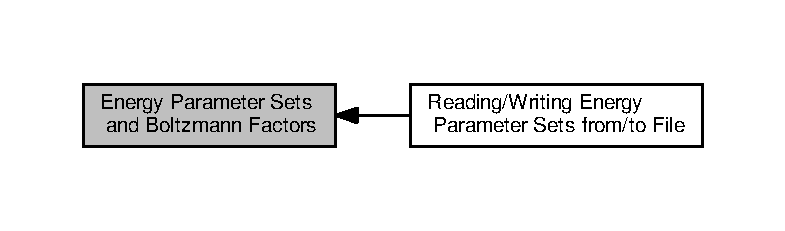
\includegraphics[width=350pt]{group__energy__parameters}
\end{center}
\end{figure}
\subsection*{Modules}
\begin{DoxyCompactItemize}
\item 
\hyperlink{group__energy__parameters__rw}{Reading/\+Writing Energy Parameter Sets from/to File}
\begin{DoxyCompactList}\small\item\em Read and Write energy parameter sets from and to text files. \end{DoxyCompactList}\end{DoxyCompactItemize}
\subsection*{Files}
\begin{DoxyCompactItemize}
\item 
file \hyperlink{params_8h}{params.\+h}
\end{DoxyCompactItemize}
\subsection*{Data Structures}
\begin{DoxyCompactItemize}
\item 
struct \hyperlink{group__energy__parameters_structvrna__param__s}{vrna\+\_\+param\+\_\+s}
\begin{DoxyCompactList}\small\item\em The datastructure that contains temperature scaled energy parameters.  \hyperlink{group__energy__parameters_structvrna__param__s}{More...}\end{DoxyCompactList}\item 
struct \hyperlink{group__energy__parameters_structvrna__exp__param__s}{vrna\+\_\+exp\+\_\+param\+\_\+s}
\begin{DoxyCompactList}\small\item\em The datastructure that contains temperature scaled Boltzmann weights of the energy parameters.  \hyperlink{group__energy__parameters_structvrna__exp__param__s}{More...}\end{DoxyCompactList}\end{DoxyCompactItemize}
\subsection*{Typedefs}
\begin{DoxyCompactItemize}
\item 
\hypertarget{group__energy__parameters_ga8a69ca7d787e4fd6079914f5343a1f35}{}typedef struct \hyperlink{group__energy__parameters_structvrna__param__s}{vrna\+\_\+param\+\_\+s} \hyperlink{group__energy__parameters_ga8a69ca7d787e4fd6079914f5343a1f35}{vrna\+\_\+param\+\_\+t}\label{group__energy__parameters_ga8a69ca7d787e4fd6079914f5343a1f35}

\begin{DoxyCompactList}\small\item\em Typename for the free energy parameter data structure \hyperlink{group__energy__parameters_gad0e3e7e74bdc50d1709d40c92993185e}{vrna\+\_\+params}. \end{DoxyCompactList}\item 
\hypertarget{group__energy__parameters_ga01d8b92fe734df8d79a6169482c7d8d8}{}typedef struct \hyperlink{group__energy__parameters_structvrna__exp__param__s}{vrna\+\_\+exp\+\_\+param\+\_\+s} \hyperlink{group__energy__parameters_ga01d8b92fe734df8d79a6169482c7d8d8}{vrna\+\_\+exp\+\_\+param\+\_\+t}\label{group__energy__parameters_ga01d8b92fe734df8d79a6169482c7d8d8}

\begin{DoxyCompactList}\small\item\em Typename for the Boltzmann factor data structure \hyperlink{group__energy__parameters_gab1f3016f96aa96bff020cdd904605afa}{vrna\+\_\+exp\+\_\+params}. \end{DoxyCompactList}\item 
typedef struct \hyperlink{group__energy__parameters_structvrna__param__s}{vrna\+\_\+param\+\_\+s} \hyperlink{group__energy__parameters_ga857dde86357d306cc902f0d8b2797659}{param\+T}
\begin{DoxyCompactList}\small\item\em Old typename of \hyperlink{group__energy__parameters_structvrna__param__s}{vrna\+\_\+param\+\_\+s}. \end{DoxyCompactList}\item 
typedef struct \hyperlink{group__energy__parameters_structvrna__exp__param__s}{vrna\+\_\+exp\+\_\+param\+\_\+s} \hyperlink{group__energy__parameters_ga8bffe1828e2cbec101769f5cc0b1535b}{pf\+\_\+param\+T}
\begin{DoxyCompactList}\small\item\em Old typename of \#vrna\+\_\+ex\+\_\+param\+\_\+s. \end{DoxyCompactList}\end{DoxyCompactItemize}
\subsection*{Functions}
\begin{DoxyCompactItemize}
\item 
\hyperlink{group__energy__parameters_ga8a69ca7d787e4fd6079914f5343a1f35}{vrna\+\_\+param\+\_\+t} $\ast$ \hyperlink{group__energy__parameters_gad0e3e7e74bdc50d1709d40c92993185e}{vrna\+\_\+params} (\hyperlink{group__model__details_ga1f8a10e12a0a1915f2a4eff0b28ea17c}{vrna\+\_\+md\+\_\+t} $\ast$md)
\begin{DoxyCompactList}\small\item\em Get a data structure containing prescaled free energy parameters. \end{DoxyCompactList}\item 
\hyperlink{group__energy__parameters_ga8a69ca7d787e4fd6079914f5343a1f35}{vrna\+\_\+param\+\_\+t} $\ast$ \hyperlink{group__energy__parameters_ga4bffa39f26e7746148444dd8a8426eca}{vrna\+\_\+params\+\_\+copy} (\hyperlink{group__energy__parameters_ga8a69ca7d787e4fd6079914f5343a1f35}{vrna\+\_\+param\+\_\+t} $\ast$par)
\begin{DoxyCompactList}\small\item\em Get a copy of the provided free energy parameters. \end{DoxyCompactList}\item 
\hyperlink{group__energy__parameters_ga01d8b92fe734df8d79a6169482c7d8d8}{vrna\+\_\+exp\+\_\+param\+\_\+t} $\ast$ \hyperlink{group__energy__parameters_gab1f3016f96aa96bff020cdd904605afa}{vrna\+\_\+exp\+\_\+params} (\hyperlink{group__model__details_ga1f8a10e12a0a1915f2a4eff0b28ea17c}{vrna\+\_\+md\+\_\+t} $\ast$md)
\begin{DoxyCompactList}\small\item\em Get a data structure containing prescaled free energy parameters already transformed to Boltzmann factors. \end{DoxyCompactList}\item 
\hyperlink{group__energy__parameters_ga01d8b92fe734df8d79a6169482c7d8d8}{vrna\+\_\+exp\+\_\+param\+\_\+t} $\ast$ \hyperlink{group__energy__parameters_gaf78c09e685e6eef4100b1a41d4042550}{vrna\+\_\+exp\+\_\+params\+\_\+comparative} (unsigned int n\+\_\+seq, \hyperlink{group__model__details_ga1f8a10e12a0a1915f2a4eff0b28ea17c}{vrna\+\_\+md\+\_\+t} $\ast$md)
\begin{DoxyCompactList}\small\item\em Get a data structure containing prescaled free energy parameters already transformed to Boltzmann factors (alifold version) \end{DoxyCompactList}\item 
\hyperlink{group__energy__parameters_ga01d8b92fe734df8d79a6169482c7d8d8}{vrna\+\_\+exp\+\_\+param\+\_\+t} $\ast$ \hyperlink{group__energy__parameters_ga70bc46be7cfa5434a71efe241c4f0609}{vrna\+\_\+exp\+\_\+params\+\_\+copy} (\hyperlink{group__energy__parameters_ga01d8b92fe734df8d79a6169482c7d8d8}{vrna\+\_\+exp\+\_\+param\+\_\+t} $\ast$par)
\begin{DoxyCompactList}\small\item\em Get a copy of the provided free energy parameters (provided as Boltzmann factors) \end{DoxyCompactList}\item 
void \hyperlink{group__energy__parameters_ga5d1909208f7ea3baa98b75afaa1f62ca}{vrna\+\_\+params\+\_\+subst} (\hyperlink{group__fold__compound_ga1b0cef17fd40466cef5968eaeeff6166}{vrna\+\_\+fold\+\_\+compound\+\_\+t} $\ast$vc, \hyperlink{group__energy__parameters_ga8a69ca7d787e4fd6079914f5343a1f35}{vrna\+\_\+param\+\_\+t} $\ast$par)
\begin{DoxyCompactList}\small\item\em Update/\+Reset energy parameters data structure within a \hyperlink{group__fold__compound_ga1b0cef17fd40466cef5968eaeeff6166}{vrna\+\_\+fold\+\_\+compound\+\_\+t}. \end{DoxyCompactList}\item 
void \hyperlink{group__energy__parameters_ga8e7ac4fab3b0cc03afbc134eaafb3525}{vrna\+\_\+exp\+\_\+params\+\_\+subst} (\hyperlink{group__fold__compound_ga1b0cef17fd40466cef5968eaeeff6166}{vrna\+\_\+fold\+\_\+compound\+\_\+t} $\ast$vc, \hyperlink{group__energy__parameters_ga01d8b92fe734df8d79a6169482c7d8d8}{vrna\+\_\+exp\+\_\+param\+\_\+t} $\ast$params)
\begin{DoxyCompactList}\small\item\em Update the energy parameters for subsequent partition function computations. \end{DoxyCompactList}\item 
void \hyperlink{group__energy__parameters_gad607bc3a5b5da16400e2ca4ea5560233}{vrna\+\_\+exp\+\_\+params\+\_\+rescale} (\hyperlink{group__fold__compound_ga1b0cef17fd40466cef5968eaeeff6166}{vrna\+\_\+fold\+\_\+compound\+\_\+t} $\ast$vc, double $\ast$mfe)
\begin{DoxyCompactList}\small\item\em Rescale Boltzmann factors for partition function computations. \end{DoxyCompactList}\item 
void \hyperlink{group__energy__parameters_gac40dc82e48a72a97cfc58b9da08a7792}{vrna\+\_\+params\+\_\+reset} (\hyperlink{group__fold__compound_ga1b0cef17fd40466cef5968eaeeff6166}{vrna\+\_\+fold\+\_\+compound\+\_\+t} $\ast$vc, \hyperlink{group__model__details_ga1f8a10e12a0a1915f2a4eff0b28ea17c}{vrna\+\_\+md\+\_\+t} $\ast$md\+\_\+p)
\begin{DoxyCompactList}\small\item\em Reset free energy parameters within a \hyperlink{group__fold__compound_ga1b0cef17fd40466cef5968eaeeff6166}{vrna\+\_\+fold\+\_\+compound\+\_\+t} according to provided, or default model details. \end{DoxyCompactList}\item 
void \hyperlink{group__energy__parameters_gae3c6f8897fb1f824e7fa55ab179aa3e8}{vrna\+\_\+exp\+\_\+params\+\_\+reset} (\hyperlink{group__fold__compound_ga1b0cef17fd40466cef5968eaeeff6166}{vrna\+\_\+fold\+\_\+compound\+\_\+t} $\ast$vc, \hyperlink{group__model__details_ga1f8a10e12a0a1915f2a4eff0b28ea17c}{vrna\+\_\+md\+\_\+t} $\ast$md\+\_\+p)
\begin{DoxyCompactList}\small\item\em Reset Boltzmann factors for partition function computations within a \hyperlink{group__fold__compound_ga1b0cef17fd40466cef5968eaeeff6166}{vrna\+\_\+fold\+\_\+compound\+\_\+t} according to provided, or default model details. \end{DoxyCompactList}\item 
\hyperlink{group__energy__parameters_ga01d8b92fe734df8d79a6169482c7d8d8}{vrna\+\_\+exp\+\_\+param\+\_\+t} $\ast$ \hyperlink{group__energy__parameters_gabf3b9271c41dd3fac02d56e0b02b3344}{get\+\_\+scaled\+\_\+pf\+\_\+parameters} (void)
\item 
\hyperlink{group__energy__parameters_ga01d8b92fe734df8d79a6169482c7d8d8}{vrna\+\_\+exp\+\_\+param\+\_\+t} $\ast$ \hyperlink{group__energy__parameters_gaef2b931c7e9d4ffb0a5c33df50ec2068}{get\+\_\+boltzmann\+\_\+factors} (double \hyperlink{group__model__details_gab4b11c8d9c758430960896bc3fe82ead}{temperature}, double beta\+Scale, \hyperlink{group__model__details_ga1f8a10e12a0a1915f2a4eff0b28ea17c}{vrna\+\_\+md\+\_\+t} md, double \hyperlink{group__model__details_gad3b22044065acc6dee0af68931b52cfd}{pf\+\_\+scale})
\begin{DoxyCompactList}\small\item\em Get precomputed Boltzmann factors of the loop type dependent energy contributions with independent thermodynamic temperature. \end{DoxyCompactList}\item 
\hyperlink{group__energy__parameters_ga01d8b92fe734df8d79a6169482c7d8d8}{vrna\+\_\+exp\+\_\+param\+\_\+t} $\ast$ \hyperlink{group__energy__parameters_ga665a446ba8ff211e551297a8fa36ec27}{get\+\_\+boltzmann\+\_\+factor\+\_\+copy} (\hyperlink{group__energy__parameters_ga01d8b92fe734df8d79a6169482c7d8d8}{vrna\+\_\+exp\+\_\+param\+\_\+t} $\ast$parameters)
\begin{DoxyCompactList}\small\item\em Get a copy of already precomputed Boltzmann factors. \end{DoxyCompactList}\item 
\hyperlink{group__energy__parameters_ga01d8b92fe734df8d79a6169482c7d8d8}{vrna\+\_\+exp\+\_\+param\+\_\+t} $\ast$ \hyperlink{group__energy__parameters_ga0ccf4e1be085a573533fd6b9da2d8cf9}{get\+\_\+scaled\+\_\+alipf\+\_\+parameters} (unsigned int n\+\_\+seq)
\begin{DoxyCompactList}\small\item\em Get precomputed Boltzmann factors of the loop type dependent energy contributions (alifold variant) \end{DoxyCompactList}\item 
\hyperlink{group__energy__parameters_ga01d8b92fe734df8d79a6169482c7d8d8}{vrna\+\_\+exp\+\_\+param\+\_\+t} $\ast$ \hyperlink{group__energy__parameters_ga2aa1d87c97f35d2e4121634a17556829}{get\+\_\+boltzmann\+\_\+factors\+\_\+ali} (unsigned int n\+\_\+seq, double \hyperlink{group__model__details_gab4b11c8d9c758430960896bc3fe82ead}{temperature}, double beta\+Scale, \hyperlink{group__model__details_ga1f8a10e12a0a1915f2a4eff0b28ea17c}{vrna\+\_\+md\+\_\+t} md, double \hyperlink{group__model__details_gad3b22044065acc6dee0af68931b52cfd}{pf\+\_\+scale})
\begin{DoxyCompactList}\small\item\em Get precomputed Boltzmann factors of the loop type dependent energy contributions (alifold variant) with independent thermodynamic temperature. \end{DoxyCompactList}\item 
\hyperlink{group__energy__parameters_ga8a69ca7d787e4fd6079914f5343a1f35}{vrna\+\_\+param\+\_\+t} $\ast$ \hyperlink{group__energy__parameters_ga541f2cf7436e9bc939b0a49b24baf987}{scale\+\_\+parameters} (void)
\begin{DoxyCompactList}\small\item\em Get precomputed energy contributions for all the known loop types. \end{DoxyCompactList}\item 
\hyperlink{group__energy__parameters_ga8a69ca7d787e4fd6079914f5343a1f35}{vrna\+\_\+param\+\_\+t} $\ast$ \hyperlink{group__energy__parameters_ga7fa6a000d7c16feab939f2c4ee626197}{get\+\_\+scaled\+\_\+parameters} (double \hyperlink{group__model__details_gab4b11c8d9c758430960896bc3fe82ead}{temperature}, \hyperlink{group__model__details_ga1f8a10e12a0a1915f2a4eff0b28ea17c}{vrna\+\_\+md\+\_\+t} md)
\begin{DoxyCompactList}\small\item\em Get precomputed energy contributions for all the known loop types. \end{DoxyCompactList}\end{DoxyCompactItemize}


\subsection{Detailed Description}
All relevant functions to retrieve and copy precalculated energy parameter sets as well as reading/writing the energy parameter set from/to file(s). 

This module covers all relevant functions for precalculation of the energy parameters necessary for the folding routines provided by R\+N\+Alib. Furthermore, the energy parameter set in the R\+N\+Alib can be easily exchanged by a user-\/defined one. It is also possible to write the current energy parameter set into a text file. 

\subsection{Data Structure Documentation}
\index{vrna\+\_\+param\+\_\+s@{vrna\+\_\+param\+\_\+s}}\label{structvrna__param__s}
\hypertarget{group__energy__parameters_structvrna__param__s}{}
\subsubsection{struct vrna\+\_\+param\+\_\+s}
The datastructure that contains temperature scaled energy parameters. 

Collaboration diagram for vrna\+\_\+param\+\_\+s\+:
\nopagebreak
\begin{figure}[H]
\begin{center}
\leavevmode
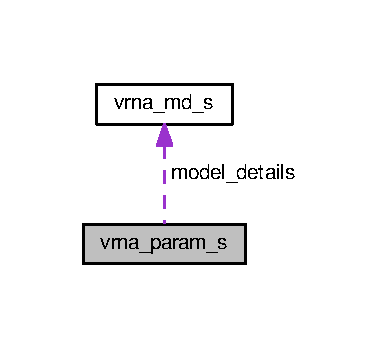
\includegraphics[width=183pt]{structvrna__param__s__coll__graph}
\end{center}
\end{figure}
\subsubsection*{Data Fields}
\begin{DoxyCompactItemize}
\item 
\hypertarget{group__energy__parameters_aeed2cd83713012bcb52e431041e037c8}{}double \hyperlink{group__energy__parameters_aeed2cd83713012bcb52e431041e037c8}{temperature}\label{group__energy__parameters_aeed2cd83713012bcb52e431041e037c8}

\begin{DoxyCompactList}\small\item\em Temperature used for loop contribution scaling. \end{DoxyCompactList}\item 
\hypertarget{group__energy__parameters_a7b84353eb9075c595bad4ceb871bcae7}{}\hyperlink{group__model__details_ga1f8a10e12a0a1915f2a4eff0b28ea17c}{vrna\+\_\+md\+\_\+t} \hyperlink{group__energy__parameters_a7b84353eb9075c595bad4ceb871bcae7}{model\+\_\+details}\label{group__energy__parameters_a7b84353eb9075c595bad4ceb871bcae7}

\begin{DoxyCompactList}\small\item\em Model details to be used in the recursions. \end{DoxyCompactList}\end{DoxyCompactItemize}
\index{vrna\+\_\+exp\+\_\+param\+\_\+s@{vrna\+\_\+exp\+\_\+param\+\_\+s}}\label{structvrna__exp__param__s}
\hypertarget{group__energy__parameters_structvrna__exp__param__s}{}
\subsubsection{struct vrna\+\_\+exp\+\_\+param\+\_\+s}
The datastructure that contains temperature scaled Boltzmann weights of the energy parameters. 

Collaboration diagram for vrna\+\_\+exp\+\_\+param\+\_\+s\+:
\nopagebreak
\begin{figure}[H]
\begin{center}
\leavevmode
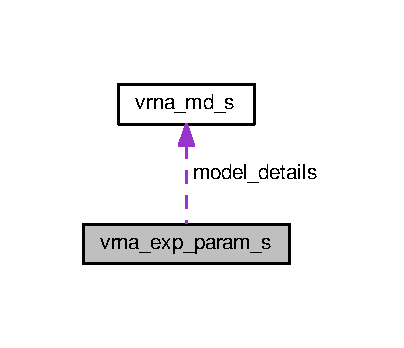
\includegraphics[width=194pt]{structvrna__exp__param__s__coll__graph}
\end{center}
\end{figure}
\subsubsection*{Data Fields}
\begin{DoxyCompactItemize}
\item 
int \hyperlink{group__energy__parameters_a378d5bcf2bae1f3ec84c912c7d3908d2}{id}
\begin{DoxyCompactList}\small\item\em An identifier for the data structure. \end{DoxyCompactList}\item 
\hypertarget{group__energy__parameters_a53c12f0d74f94ce371e0471a8ab5a377}{}double \hyperlink{group__energy__parameters_a53c12f0d74f94ce371e0471a8ab5a377}{pf\+\_\+scale}\label{group__energy__parameters_a53c12f0d74f94ce371e0471a8ab5a377}

\begin{DoxyCompactList}\small\item\em Scaling factor to avoid over-\//underflows. \end{DoxyCompactList}\item 
\hypertarget{group__energy__parameters_a674656d65ea957ddbeff8bd146b7fc16}{}double \hyperlink{group__energy__parameters_a674656d65ea957ddbeff8bd146b7fc16}{temperature}\label{group__energy__parameters_a674656d65ea957ddbeff8bd146b7fc16}

\begin{DoxyCompactList}\small\item\em Temperature used for loop contribution scaling. \end{DoxyCompactList}\item 
double \hyperlink{group__energy__parameters_a77145830b7bb01b36c3217b363310ef0}{alpha}
\begin{DoxyCompactList}\small\item\em Scaling factor for the thermodynamic temperature. \end{DoxyCompactList}\item 
\hypertarget{group__energy__parameters_ac18055127bccc27c1223f1d2f3b01b53}{}\hyperlink{group__model__details_ga1f8a10e12a0a1915f2a4eff0b28ea17c}{vrna\+\_\+md\+\_\+t} \hyperlink{group__energy__parameters_ac18055127bccc27c1223f1d2f3b01b53}{model\+\_\+details}\label{group__energy__parameters_ac18055127bccc27c1223f1d2f3b01b53}

\begin{DoxyCompactList}\small\item\em Model details to be used in the recursions. \end{DoxyCompactList}\end{DoxyCompactItemize}


\paragraph{Field Documentation}
\hypertarget{group__energy__parameters_a378d5bcf2bae1f3ec84c912c7d3908d2}{}\index{vrna\+\_\+exp\+\_\+param\+\_\+s@{vrna\+\_\+exp\+\_\+param\+\_\+s}!id@{id}}
\index{id@{id}!vrna\+\_\+exp\+\_\+param\+\_\+s@{vrna\+\_\+exp\+\_\+param\+\_\+s}}
\subparagraph[{id}]{\setlength{\rightskip}{0pt plus 5cm}int vrna\+\_\+exp\+\_\+param\+\_\+s\+::id}\label{group__energy__parameters_a378d5bcf2bae1f3ec84c912c7d3908d2}


An identifier for the data structure. 

\begin{DoxyRefDesc}{Deprecated}
\item[\hyperlink{deprecated__deprecated000099}{Deprecated}]This attribute will be removed in version 3 \end{DoxyRefDesc}
\hypertarget{group__energy__parameters_a77145830b7bb01b36c3217b363310ef0}{}\index{vrna\+\_\+exp\+\_\+param\+\_\+s@{vrna\+\_\+exp\+\_\+param\+\_\+s}!alpha@{alpha}}
\index{alpha@{alpha}!vrna\+\_\+exp\+\_\+param\+\_\+s@{vrna\+\_\+exp\+\_\+param\+\_\+s}}
\subparagraph[{alpha}]{\setlength{\rightskip}{0pt plus 5cm}double vrna\+\_\+exp\+\_\+param\+\_\+s\+::alpha}\label{group__energy__parameters_a77145830b7bb01b36c3217b363310ef0}


Scaling factor for the thermodynamic temperature. 

This allows for temperature scaling in Boltzmann factors independently from the energy contributions. The resulting Boltzmann factors are then computed by $ e^{-E/(\alpha \cdot K \cdot T)} $ 

\subsection{Typedef Documentation}
\hypertarget{group__energy__parameters_ga857dde86357d306cc902f0d8b2797659}{}\index{Energy Parameter Sets and Boltzmann Factors@{Energy Parameter Sets and Boltzmann Factors}!param\+T@{param\+T}}
\index{param\+T@{param\+T}!Energy Parameter Sets and Boltzmann Factors@{Energy Parameter Sets and Boltzmann Factors}}
\subsubsection[{param\+T}]{\setlength{\rightskip}{0pt plus 5cm}typedef struct {\bf vrna\+\_\+param\+\_\+s} {\bf param\+T}}\label{group__energy__parameters_ga857dde86357d306cc902f0d8b2797659}


{\ttfamily \#include $<$\hyperlink{params_8h}{Vienna\+R\+N\+A/params.\+h}$>$}



Old typename of \hyperlink{group__energy__parameters_structvrna__param__s}{vrna\+\_\+param\+\_\+s}. 

\begin{DoxyRefDesc}{Deprecated}
\item[\hyperlink{deprecated__deprecated000090}{Deprecated}]Use \hyperlink{group__energy__parameters_ga8a69ca7d787e4fd6079914f5343a1f35}{vrna\+\_\+param\+\_\+t} instead! \end{DoxyRefDesc}
\hypertarget{group__energy__parameters_ga8bffe1828e2cbec101769f5cc0b1535b}{}\index{Energy Parameter Sets and Boltzmann Factors@{Energy Parameter Sets and Boltzmann Factors}!pf\+\_\+param\+T@{pf\+\_\+param\+T}}
\index{pf\+\_\+param\+T@{pf\+\_\+param\+T}!Energy Parameter Sets and Boltzmann Factors@{Energy Parameter Sets and Boltzmann Factors}}
\subsubsection[{pf\+\_\+param\+T}]{\setlength{\rightskip}{0pt plus 5cm}typedef struct {\bf vrna\+\_\+exp\+\_\+param\+\_\+s} {\bf pf\+\_\+param\+T}}\label{group__energy__parameters_ga8bffe1828e2cbec101769f5cc0b1535b}


{\ttfamily \#include $<$\hyperlink{params_8h}{Vienna\+R\+N\+A/params.\+h}$>$}



Old typename of \#vrna\+\_\+ex\+\_\+param\+\_\+s. 

\begin{DoxyRefDesc}{Deprecated}
\item[\hyperlink{deprecated__deprecated000091}{Deprecated}]Use \hyperlink{group__energy__parameters_ga01d8b92fe734df8d79a6169482c7d8d8}{vrna\+\_\+exp\+\_\+param\+\_\+t} instead! \end{DoxyRefDesc}


\subsection{Function Documentation}
\hypertarget{group__energy__parameters_gad0e3e7e74bdc50d1709d40c92993185e}{}\index{Energy Parameter Sets and Boltzmann Factors@{Energy Parameter Sets and Boltzmann Factors}!vrna\+\_\+params@{vrna\+\_\+params}}
\index{vrna\+\_\+params@{vrna\+\_\+params}!Energy Parameter Sets and Boltzmann Factors@{Energy Parameter Sets and Boltzmann Factors}}
\subsubsection[{vrna\+\_\+params}]{\setlength{\rightskip}{0pt plus 5cm}{\bf vrna\+\_\+param\+\_\+t}$\ast$ vrna\+\_\+params (
\begin{DoxyParamCaption}
\item[{{\bf vrna\+\_\+md\+\_\+t} $\ast$}]{md}
\end{DoxyParamCaption}
)}\label{group__energy__parameters_gad0e3e7e74bdc50d1709d40c92993185e}


{\ttfamily \#include $<$\hyperlink{params_8h}{Vienna\+R\+N\+A/params.\+h}$>$}



Get a data structure containing prescaled free energy parameters. 

If a N\+U\+L\+L pointer is passed for the model details parameter, the default model parameters are stored within the requested \hyperlink{group__energy__parameters_ga8a69ca7d787e4fd6079914f5343a1f35}{vrna\+\_\+param\+\_\+t} structure.

\begin{DoxySeeAlso}{See also}
\hyperlink{group__model__details_ga1f8a10e12a0a1915f2a4eff0b28ea17c}{vrna\+\_\+md\+\_\+t}, \hyperlink{group__model__details_ga8ac6ff84936282436f822644bf841f66}{vrna\+\_\+md\+\_\+set\+\_\+default()}, \hyperlink{group__energy__parameters_gab1f3016f96aa96bff020cdd904605afa}{vrna\+\_\+exp\+\_\+params()}
\end{DoxySeeAlso}

\begin{DoxyParams}{Parameters}
{\em md} & A pointer to the model details to store inside the structure (Maybe N\+U\+L\+L) \\
\hline
\end{DoxyParams}
\begin{DoxyReturn}{Returns}
A pointer to the memory location where the requested parameters are stored 
\end{DoxyReturn}
\hypertarget{group__energy__parameters_ga4bffa39f26e7746148444dd8a8426eca}{}\index{Energy Parameter Sets and Boltzmann Factors@{Energy Parameter Sets and Boltzmann Factors}!vrna\+\_\+params\+\_\+copy@{vrna\+\_\+params\+\_\+copy}}
\index{vrna\+\_\+params\+\_\+copy@{vrna\+\_\+params\+\_\+copy}!Energy Parameter Sets and Boltzmann Factors@{Energy Parameter Sets and Boltzmann Factors}}
\subsubsection[{vrna\+\_\+params\+\_\+copy}]{\setlength{\rightskip}{0pt plus 5cm}{\bf vrna\+\_\+param\+\_\+t}$\ast$ vrna\+\_\+params\+\_\+copy (
\begin{DoxyParamCaption}
\item[{{\bf vrna\+\_\+param\+\_\+t} $\ast$}]{par}
\end{DoxyParamCaption}
)}\label{group__energy__parameters_ga4bffa39f26e7746148444dd8a8426eca}


{\ttfamily \#include $<$\hyperlink{params_8h}{Vienna\+R\+N\+A/params.\+h}$>$}



Get a copy of the provided free energy parameters. 

If N\+U\+L\+L is passed as parameter, a default set of energy parameters is created and returned.

\begin{DoxySeeAlso}{See also}
\hyperlink{group__energy__parameters_gad0e3e7e74bdc50d1709d40c92993185e}{vrna\+\_\+params()}, \hyperlink{group__energy__parameters_ga8a69ca7d787e4fd6079914f5343a1f35}{vrna\+\_\+param\+\_\+t}
\end{DoxySeeAlso}

\begin{DoxyParams}{Parameters}
{\em par} & The free energy parameters that are to be copied (Maybe N\+U\+L\+L) \\
\hline
\end{DoxyParams}
\begin{DoxyReturn}{Returns}
A copy or a default set of the (provided) parameters 
\end{DoxyReturn}
\hypertarget{group__energy__parameters_gab1f3016f96aa96bff020cdd904605afa}{}\index{Energy Parameter Sets and Boltzmann Factors@{Energy Parameter Sets and Boltzmann Factors}!vrna\+\_\+exp\+\_\+params@{vrna\+\_\+exp\+\_\+params}}
\index{vrna\+\_\+exp\+\_\+params@{vrna\+\_\+exp\+\_\+params}!Energy Parameter Sets and Boltzmann Factors@{Energy Parameter Sets and Boltzmann Factors}}
\subsubsection[{vrna\+\_\+exp\+\_\+params}]{\setlength{\rightskip}{0pt plus 5cm}{\bf vrna\+\_\+exp\+\_\+param\+\_\+t}$\ast$ vrna\+\_\+exp\+\_\+params (
\begin{DoxyParamCaption}
\item[{{\bf vrna\+\_\+md\+\_\+t} $\ast$}]{md}
\end{DoxyParamCaption}
)}\label{group__energy__parameters_gab1f3016f96aa96bff020cdd904605afa}


{\ttfamily \#include $<$\hyperlink{params_8h}{Vienna\+R\+N\+A/params.\+h}$>$}



Get a data structure containing prescaled free energy parameters already transformed to Boltzmann factors. 

This function returns a data structure that contains all necessary precomputed energy contributions for each type of loop.

In contrast to \hyperlink{group__energy__parameters_gad0e3e7e74bdc50d1709d40c92993185e}{vrna\+\_\+params()}, the free energies within this data structure are stored as their Boltzmann factors, i.\+e.

$ exp(-E / kT) $

where $ E $ is the free energy.

If a N\+U\+L\+L pointer is passed for the model details parameter, the default model parameters are stored within the requested \hyperlink{group__energy__parameters_ga01d8b92fe734df8d79a6169482c7d8d8}{vrna\+\_\+exp\+\_\+param\+\_\+t} structure.

\begin{DoxySeeAlso}{See also}
\hyperlink{group__model__details_ga1f8a10e12a0a1915f2a4eff0b28ea17c}{vrna\+\_\+md\+\_\+t}, \hyperlink{group__model__details_ga8ac6ff84936282436f822644bf841f66}{vrna\+\_\+md\+\_\+set\+\_\+default()}, \hyperlink{group__energy__parameters_gad0e3e7e74bdc50d1709d40c92993185e}{vrna\+\_\+params()}, vrna\+\_\+rescale\+\_\+pf\+\_\+params()
\end{DoxySeeAlso}

\begin{DoxyParams}{Parameters}
{\em md} & A pointer to the model details to store inside the structure (Maybe N\+U\+L\+L) \\
\hline
\end{DoxyParams}
\begin{DoxyReturn}{Returns}
A pointer to the memory location where the requested parameters are stored 
\end{DoxyReturn}
\hypertarget{group__energy__parameters_gaf78c09e685e6eef4100b1a41d4042550}{}\index{Energy Parameter Sets and Boltzmann Factors@{Energy Parameter Sets and Boltzmann Factors}!vrna\+\_\+exp\+\_\+params\+\_\+comparative@{vrna\+\_\+exp\+\_\+params\+\_\+comparative}}
\index{vrna\+\_\+exp\+\_\+params\+\_\+comparative@{vrna\+\_\+exp\+\_\+params\+\_\+comparative}!Energy Parameter Sets and Boltzmann Factors@{Energy Parameter Sets and Boltzmann Factors}}
\subsubsection[{vrna\+\_\+exp\+\_\+params\+\_\+comparative}]{\setlength{\rightskip}{0pt plus 5cm}{\bf vrna\+\_\+exp\+\_\+param\+\_\+t}$\ast$ vrna\+\_\+exp\+\_\+params\+\_\+comparative (
\begin{DoxyParamCaption}
\item[{unsigned int}]{n\+\_\+seq, }
\item[{{\bf vrna\+\_\+md\+\_\+t} $\ast$}]{md}
\end{DoxyParamCaption}
)}\label{group__energy__parameters_gaf78c09e685e6eef4100b1a41d4042550}


{\ttfamily \#include $<$\hyperlink{params_8h}{Vienna\+R\+N\+A/params.\+h}$>$}



Get a data structure containing prescaled free energy parameters already transformed to Boltzmann factors (alifold version) 

If a N\+U\+L\+L pointer is passed for the model details parameter, the default model parameters are stored within the requested \hyperlink{group__energy__parameters_ga01d8b92fe734df8d79a6169482c7d8d8}{vrna\+\_\+exp\+\_\+param\+\_\+t} structure.

\begin{DoxySeeAlso}{See also}
\hyperlink{group__model__details_ga1f8a10e12a0a1915f2a4eff0b28ea17c}{vrna\+\_\+md\+\_\+t}, \hyperlink{group__model__details_ga8ac6ff84936282436f822644bf841f66}{vrna\+\_\+md\+\_\+set\+\_\+default()}, \hyperlink{group__energy__parameters_gab1f3016f96aa96bff020cdd904605afa}{vrna\+\_\+exp\+\_\+params()}, \hyperlink{group__energy__parameters_gad0e3e7e74bdc50d1709d40c92993185e}{vrna\+\_\+params()}
\end{DoxySeeAlso}

\begin{DoxyParams}{Parameters}
{\em n\+\_\+seq} & The number of sequences in the alignment \\
\hline
{\em md} & A pointer to the model details to store inside the structure (Maybe N\+U\+L\+L) \\
\hline
\end{DoxyParams}
\begin{DoxyReturn}{Returns}
A pointer to the memory location where the requested parameters are stored 
\end{DoxyReturn}
\hypertarget{group__energy__parameters_ga70bc46be7cfa5434a71efe241c4f0609}{}\index{Energy Parameter Sets and Boltzmann Factors@{Energy Parameter Sets and Boltzmann Factors}!vrna\+\_\+exp\+\_\+params\+\_\+copy@{vrna\+\_\+exp\+\_\+params\+\_\+copy}}
\index{vrna\+\_\+exp\+\_\+params\+\_\+copy@{vrna\+\_\+exp\+\_\+params\+\_\+copy}!Energy Parameter Sets and Boltzmann Factors@{Energy Parameter Sets and Boltzmann Factors}}
\subsubsection[{vrna\+\_\+exp\+\_\+params\+\_\+copy}]{\setlength{\rightskip}{0pt plus 5cm}{\bf vrna\+\_\+exp\+\_\+param\+\_\+t}$\ast$ vrna\+\_\+exp\+\_\+params\+\_\+copy (
\begin{DoxyParamCaption}
\item[{{\bf vrna\+\_\+exp\+\_\+param\+\_\+t} $\ast$}]{par}
\end{DoxyParamCaption}
)}\label{group__energy__parameters_ga70bc46be7cfa5434a71efe241c4f0609}


{\ttfamily \#include $<$\hyperlink{params_8h}{Vienna\+R\+N\+A/params.\+h}$>$}



Get a copy of the provided free energy parameters (provided as Boltzmann factors) 

If N\+U\+L\+L is passed as parameter, a default set of energy parameters is created and returned.

\begin{DoxySeeAlso}{See also}
\hyperlink{group__energy__parameters_gab1f3016f96aa96bff020cdd904605afa}{vrna\+\_\+exp\+\_\+params()}, \hyperlink{group__energy__parameters_ga01d8b92fe734df8d79a6169482c7d8d8}{vrna\+\_\+exp\+\_\+param\+\_\+t}
\end{DoxySeeAlso}

\begin{DoxyParams}{Parameters}
{\em par} & The free energy parameters that are to be copied (Maybe N\+U\+L\+L) \\
\hline
\end{DoxyParams}
\begin{DoxyReturn}{Returns}
A copy or a default set of the (provided) parameters 
\end{DoxyReturn}
\hypertarget{group__energy__parameters_ga5d1909208f7ea3baa98b75afaa1f62ca}{}\index{Energy Parameter Sets and Boltzmann Factors@{Energy Parameter Sets and Boltzmann Factors}!vrna\+\_\+params\+\_\+subst@{vrna\+\_\+params\+\_\+subst}}
\index{vrna\+\_\+params\+\_\+subst@{vrna\+\_\+params\+\_\+subst}!Energy Parameter Sets and Boltzmann Factors@{Energy Parameter Sets and Boltzmann Factors}}
\subsubsection[{vrna\+\_\+params\+\_\+subst}]{\setlength{\rightskip}{0pt plus 5cm}void vrna\+\_\+params\+\_\+subst (
\begin{DoxyParamCaption}
\item[{{\bf vrna\+\_\+fold\+\_\+compound\+\_\+t} $\ast$}]{vc, }
\item[{{\bf vrna\+\_\+param\+\_\+t} $\ast$}]{par}
\end{DoxyParamCaption}
)}\label{group__energy__parameters_ga5d1909208f7ea3baa98b75afaa1f62ca}


{\ttfamily \#include $<$\hyperlink{params_8h}{Vienna\+R\+N\+A/params.\+h}$>$}



Update/\+Reset energy parameters data structure within a \hyperlink{group__fold__compound_ga1b0cef17fd40466cef5968eaeeff6166}{vrna\+\_\+fold\+\_\+compound\+\_\+t}. 

Passing N\+U\+L\+L as second argument leads to a reset of the energy parameters within vc to their default values. Otherwise, the energy parameters provided will be copied over into vc.

\begin{DoxySeeAlso}{See also}
\hyperlink{group__energy__parameters_gac40dc82e48a72a97cfc58b9da08a7792}{vrna\+\_\+params\+\_\+reset()}, \hyperlink{group__energy__parameters_ga8a69ca7d787e4fd6079914f5343a1f35}{vrna\+\_\+param\+\_\+t}, \hyperlink{group__model__details_ga1f8a10e12a0a1915f2a4eff0b28ea17c}{vrna\+\_\+md\+\_\+t}, \hyperlink{group__energy__parameters_gad0e3e7e74bdc50d1709d40c92993185e}{vrna\+\_\+params()}
\end{DoxySeeAlso}

\begin{DoxyParams}{Parameters}
{\em vc} & The \hyperlink{group__fold__compound_ga1b0cef17fd40466cef5968eaeeff6166}{vrna\+\_\+fold\+\_\+compound\+\_\+t} that is about to receive updated energy parameters \\
\hline
{\em par} & The energy parameters used to substitute those within vc (Maybe N\+U\+L\+L) \\
\hline
\end{DoxyParams}
\hypertarget{group__energy__parameters_ga8e7ac4fab3b0cc03afbc134eaafb3525}{}\index{Energy Parameter Sets and Boltzmann Factors@{Energy Parameter Sets and Boltzmann Factors}!vrna\+\_\+exp\+\_\+params\+\_\+subst@{vrna\+\_\+exp\+\_\+params\+\_\+subst}}
\index{vrna\+\_\+exp\+\_\+params\+\_\+subst@{vrna\+\_\+exp\+\_\+params\+\_\+subst}!Energy Parameter Sets and Boltzmann Factors@{Energy Parameter Sets and Boltzmann Factors}}
\subsubsection[{vrna\+\_\+exp\+\_\+params\+\_\+subst}]{\setlength{\rightskip}{0pt plus 5cm}void vrna\+\_\+exp\+\_\+params\+\_\+subst (
\begin{DoxyParamCaption}
\item[{{\bf vrna\+\_\+fold\+\_\+compound\+\_\+t} $\ast$}]{vc, }
\item[{{\bf vrna\+\_\+exp\+\_\+param\+\_\+t} $\ast$}]{params}
\end{DoxyParamCaption}
)}\label{group__energy__parameters_ga8e7ac4fab3b0cc03afbc134eaafb3525}


{\ttfamily \#include $<$\hyperlink{params_8h}{Vienna\+R\+N\+A/params.\+h}$>$}



Update the energy parameters for subsequent partition function computations. 

This function can be used to properly assign new energy parameters for partition function computations to a \hyperlink{group__fold__compound_ga1b0cef17fd40466cef5968eaeeff6166}{vrna\+\_\+fold\+\_\+compound\+\_\+t}. For this purpose, the data of the provided pointer {\ttfamily params} will be copied into {\ttfamily vc} and a recomputation of the partition function scaling factor is issued, if the {\ttfamily pf\+\_\+scale} attribute of {\ttfamily params} is less than {\ttfamily 1.\+0}.

Passing N\+U\+L\+L as second argument leads to a reset of the energy parameters within vc to their default values

\begin{DoxySeeAlso}{See also}
\hyperlink{group__energy__parameters_gae3c6f8897fb1f824e7fa55ab179aa3e8}{vrna\+\_\+exp\+\_\+params\+\_\+reset()}, \hyperlink{group__energy__parameters_gad607bc3a5b5da16400e2ca4ea5560233}{vrna\+\_\+exp\+\_\+params\+\_\+rescale()}, \hyperlink{group__energy__parameters_ga01d8b92fe734df8d79a6169482c7d8d8}{vrna\+\_\+exp\+\_\+param\+\_\+t}, \hyperlink{group__model__details_ga1f8a10e12a0a1915f2a4eff0b28ea17c}{vrna\+\_\+md\+\_\+t}, \hyperlink{group__energy__parameters_gab1f3016f96aa96bff020cdd904605afa}{vrna\+\_\+exp\+\_\+params()}
\end{DoxySeeAlso}

\begin{DoxyParams}{Parameters}
{\em vc} & The fold compound data structure \\
\hline
{\em params} & A pointer to the new energy parameters \\
\hline
\end{DoxyParams}
\hypertarget{group__energy__parameters_gad607bc3a5b5da16400e2ca4ea5560233}{}\index{Energy Parameter Sets and Boltzmann Factors@{Energy Parameter Sets and Boltzmann Factors}!vrna\+\_\+exp\+\_\+params\+\_\+rescale@{vrna\+\_\+exp\+\_\+params\+\_\+rescale}}
\index{vrna\+\_\+exp\+\_\+params\+\_\+rescale@{vrna\+\_\+exp\+\_\+params\+\_\+rescale}!Energy Parameter Sets and Boltzmann Factors@{Energy Parameter Sets and Boltzmann Factors}}
\subsubsection[{vrna\+\_\+exp\+\_\+params\+\_\+rescale}]{\setlength{\rightskip}{0pt plus 5cm}void vrna\+\_\+exp\+\_\+params\+\_\+rescale (
\begin{DoxyParamCaption}
\item[{{\bf vrna\+\_\+fold\+\_\+compound\+\_\+t} $\ast$}]{vc, }
\item[{double $\ast$}]{mfe}
\end{DoxyParamCaption}
)}\label{group__energy__parameters_gad607bc3a5b5da16400e2ca4ea5560233}


{\ttfamily \#include $<$\hyperlink{params_8h}{Vienna\+R\+N\+A/params.\+h}$>$}



Rescale Boltzmann factors for partition function computations. 

This function may be used to (automatically) rescale the Boltzmann factors used in partition function computations. Since partition functions over subsequences can easily become extremely large, the R\+N\+Alib internally rescales them to avoid numerical over-\/ and/or underflow. Therefore, a proper scaling factor $s$ needs to be chosen that in turn is then used to normalize the corresponding partition functions $\hat{q}[i,j] = q[i,j] / s^{(j-i+1)}$.

This function provides two ways to automatically adjust the scaling factor.
\begin{DoxyEnumerate}
\item Automatic guess
\item Automatic adjustment according to M\+F\+E
\end{DoxyEnumerate}

Passing {\ttfamily N\+U\+L\+L} as second parameter activates the {\itshape automatic guess mode}. Here, the scaling factor is recomputed according to a mean free energy of {\ttfamily 184.\+3$\ast$length} cal for random sequences. \begin{DoxyNote}{Note}
This recomputation only takes place if the {\ttfamily pf\+\_\+scale} attribute of the {\ttfamily exp\+\_\+params} datastructure contained in {\ttfamily vc} has a value below {\ttfamily 1.\+0}.
\end{DoxyNote}
On the other hand, if the M\+F\+E for a sequence is known, it can be used to recompute a more robust scaling factor, since it represents the lowest free energy of the entire ensemble of structures, i.\+e. the highest Boltzmann factor. To activate this second mode of {\itshape automatic adjustment according to M\+F\+E}, a pointer to the M\+F\+E value needs to be passed as second argument. This value is then taken to compute the scaling factor as $ s = exp((sfact * MFE) / kT / length )$, where sfact is an additional scaling weight located in the vrna\+\_\+md\+\_\+t datastructure of {\ttfamily exp\+\_\+params} in {\ttfamily vc}.

The computed scaling factor $s$ will be stored as {\ttfamily pf\+\_\+scale} attribute of the {\ttfamily exp\+\_\+params} datastructure in {\ttfamily vc}.

\begin{DoxySeeAlso}{See also}
\hyperlink{group__energy__parameters_ga8e7ac4fab3b0cc03afbc134eaafb3525}{vrna\+\_\+exp\+\_\+params\+\_\+subst()}, \hyperlink{group__model__details_ga1f8a10e12a0a1915f2a4eff0b28ea17c}{vrna\+\_\+md\+\_\+t}, \hyperlink{group__energy__parameters_ga01d8b92fe734df8d79a6169482c7d8d8}{vrna\+\_\+exp\+\_\+param\+\_\+t}, \hyperlink{group__fold__compound_ga1b0cef17fd40466cef5968eaeeff6166}{vrna\+\_\+fold\+\_\+compound\+\_\+t}
\end{DoxySeeAlso}

\begin{DoxyParams}{Parameters}
{\em vc} & The fold compound data structure \\
\hline
{\em mfe} & A pointer to the M\+F\+E (in kcal/mol) or N\+U\+L\+L \\
\hline
\end{DoxyParams}
\hypertarget{group__energy__parameters_gac40dc82e48a72a97cfc58b9da08a7792}{}\index{Energy Parameter Sets and Boltzmann Factors@{Energy Parameter Sets and Boltzmann Factors}!vrna\+\_\+params\+\_\+reset@{vrna\+\_\+params\+\_\+reset}}
\index{vrna\+\_\+params\+\_\+reset@{vrna\+\_\+params\+\_\+reset}!Energy Parameter Sets and Boltzmann Factors@{Energy Parameter Sets and Boltzmann Factors}}
\subsubsection[{vrna\+\_\+params\+\_\+reset}]{\setlength{\rightskip}{0pt plus 5cm}void vrna\+\_\+params\+\_\+reset (
\begin{DoxyParamCaption}
\item[{{\bf vrna\+\_\+fold\+\_\+compound\+\_\+t} $\ast$}]{vc, }
\item[{{\bf vrna\+\_\+md\+\_\+t} $\ast$}]{md\+\_\+p}
\end{DoxyParamCaption}
)}\label{group__energy__parameters_gac40dc82e48a72a97cfc58b9da08a7792}


{\ttfamily \#include $<$\hyperlink{params_8h}{Vienna\+R\+N\+A/params.\+h}$>$}



Reset free energy parameters within a \hyperlink{group__fold__compound_ga1b0cef17fd40466cef5968eaeeff6166}{vrna\+\_\+fold\+\_\+compound\+\_\+t} according to provided, or default model details. 

This function allow to rescale free energy parameters for subsequent structure prediction or evaluation according to a set of model details, e.\+g. temperature values. To do so, the caller provides either a pointer to a set of model details to be used for rescaling, or N\+U\+L\+L if global default setting should be used.

\begin{DoxySeeAlso}{See also}
\hyperlink{group__energy__parameters_gae3c6f8897fb1f824e7fa55ab179aa3e8}{vrna\+\_\+exp\+\_\+params\+\_\+reset()}, vrna\+\_\+params\+\_\+subs() 
\end{DoxySeeAlso}

\begin{DoxyParams}{Parameters}
{\em vc} & The fold compound data structure \\
\hline
{\em md\+\_\+p} & A pointer to the new model details (or N\+U\+L\+L for reset to defaults) \\
\hline
\end{DoxyParams}
\hypertarget{group__energy__parameters_gae3c6f8897fb1f824e7fa55ab179aa3e8}{}\index{Energy Parameter Sets and Boltzmann Factors@{Energy Parameter Sets and Boltzmann Factors}!vrna\+\_\+exp\+\_\+params\+\_\+reset@{vrna\+\_\+exp\+\_\+params\+\_\+reset}}
\index{vrna\+\_\+exp\+\_\+params\+\_\+reset@{vrna\+\_\+exp\+\_\+params\+\_\+reset}!Energy Parameter Sets and Boltzmann Factors@{Energy Parameter Sets and Boltzmann Factors}}
\subsubsection[{vrna\+\_\+exp\+\_\+params\+\_\+reset}]{\setlength{\rightskip}{0pt plus 5cm}void vrna\+\_\+exp\+\_\+params\+\_\+reset (
\begin{DoxyParamCaption}
\item[{{\bf vrna\+\_\+fold\+\_\+compound\+\_\+t} $\ast$}]{vc, }
\item[{{\bf vrna\+\_\+md\+\_\+t} $\ast$}]{md\+\_\+p}
\end{DoxyParamCaption}
)}\label{group__energy__parameters_gae3c6f8897fb1f824e7fa55ab179aa3e8}


{\ttfamily \#include $<$\hyperlink{params_8h}{Vienna\+R\+N\+A/params.\+h}$>$}



Reset Boltzmann factors for partition function computations within a \hyperlink{group__fold__compound_ga1b0cef17fd40466cef5968eaeeff6166}{vrna\+\_\+fold\+\_\+compound\+\_\+t} according to provided, or default model details. 

This function allow to rescale Boltzmann factors for subsequent prartition function computations according to a set of model details, e.\+g. temperature values. To do so, the caller provides either a pointer to a set of model details to be used for rescaling, or N\+U\+L\+L if global default setting should be used.

\begin{DoxySeeAlso}{See also}
\hyperlink{group__energy__parameters_gac40dc82e48a72a97cfc58b9da08a7792}{vrna\+\_\+params\+\_\+reset()}, \hyperlink{group__energy__parameters_ga8e7ac4fab3b0cc03afbc134eaafb3525}{vrna\+\_\+exp\+\_\+params\+\_\+subst()}, \hyperlink{group__energy__parameters_gad607bc3a5b5da16400e2ca4ea5560233}{vrna\+\_\+exp\+\_\+params\+\_\+rescale()} 
\end{DoxySeeAlso}

\begin{DoxyParams}{Parameters}
{\em vc} & The fold compound data structure \\
\hline
{\em md\+\_\+p} & A pointer to the new model details (or N\+U\+L\+L for reset to defaults) \\
\hline
\end{DoxyParams}
\hypertarget{group__energy__parameters_gabf3b9271c41dd3fac02d56e0b02b3344}{}\index{Energy Parameter Sets and Boltzmann Factors@{Energy Parameter Sets and Boltzmann Factors}!get\+\_\+scaled\+\_\+pf\+\_\+parameters@{get\+\_\+scaled\+\_\+pf\+\_\+parameters}}
\index{get\+\_\+scaled\+\_\+pf\+\_\+parameters@{get\+\_\+scaled\+\_\+pf\+\_\+parameters}!Energy Parameter Sets and Boltzmann Factors@{Energy Parameter Sets and Boltzmann Factors}}
\subsubsection[{get\+\_\+scaled\+\_\+pf\+\_\+parameters}]{\setlength{\rightskip}{0pt plus 5cm}{\bf vrna\+\_\+exp\+\_\+param\+\_\+t}$\ast$ get\+\_\+scaled\+\_\+pf\+\_\+parameters (
\begin{DoxyParamCaption}
\item[{void}]{}
\end{DoxyParamCaption}
)}\label{group__energy__parameters_gabf3b9271c41dd3fac02d56e0b02b3344}


{\ttfamily \#include $<$\hyperlink{params_8h}{Vienna\+R\+N\+A/params.\+h}$>$}

get a datastructure of type \hyperlink{group__energy__parameters_ga01d8b92fe734df8d79a6169482c7d8d8}{vrna\+\_\+exp\+\_\+param\+\_\+t} which contains the Boltzmann weights of several energy parameters scaled according to the current temperature

\begin{DoxyRefDesc}{Deprecated}
\item[\hyperlink{deprecated__deprecated000092}{Deprecated}]Use \hyperlink{group__energy__parameters_gab1f3016f96aa96bff020cdd904605afa}{vrna\+\_\+exp\+\_\+params()} instead!\end{DoxyRefDesc}


\begin{DoxyReturn}{Returns}
The datastructure containing Boltzmann weights for use in partition function calculations 
\end{DoxyReturn}
\hypertarget{group__energy__parameters_gaef2b931c7e9d4ffb0a5c33df50ec2068}{}\index{Energy Parameter Sets and Boltzmann Factors@{Energy Parameter Sets and Boltzmann Factors}!get\+\_\+boltzmann\+\_\+factors@{get\+\_\+boltzmann\+\_\+factors}}
\index{get\+\_\+boltzmann\+\_\+factors@{get\+\_\+boltzmann\+\_\+factors}!Energy Parameter Sets and Boltzmann Factors@{Energy Parameter Sets and Boltzmann Factors}}
\subsubsection[{get\+\_\+boltzmann\+\_\+factors}]{\setlength{\rightskip}{0pt plus 5cm}{\bf vrna\+\_\+exp\+\_\+param\+\_\+t}$\ast$ get\+\_\+boltzmann\+\_\+factors (
\begin{DoxyParamCaption}
\item[{double}]{temperature, }
\item[{double}]{beta\+Scale, }
\item[{{\bf vrna\+\_\+md\+\_\+t}}]{md, }
\item[{double}]{pf\+\_\+scale}
\end{DoxyParamCaption}
)}\label{group__energy__parameters_gaef2b931c7e9d4ffb0a5c33df50ec2068}


{\ttfamily \#include $<$\hyperlink{params_8h}{Vienna\+R\+N\+A/params.\+h}$>$}



Get precomputed Boltzmann factors of the loop type dependent energy contributions with independent thermodynamic temperature. 

This function returns a data structure that contains all necessary precalculated Boltzmann factors for each loop type contribution.~\newline
 In contrast to \hyperlink{group__energy__parameters_gabf3b9271c41dd3fac02d56e0b02b3344}{get\+\_\+scaled\+\_\+pf\+\_\+parameters()}, this function enables setting of independent temperatures for both, the individual energy contributions as well as the thermodynamic temperature used in $ exp(-\Delta G / kT) $

\begin{DoxyRefDesc}{Deprecated}
\item[\hyperlink{deprecated__deprecated000093}{Deprecated}]Use \hyperlink{group__energy__parameters_gab1f3016f96aa96bff020cdd904605afa}{vrna\+\_\+exp\+\_\+params()} instead!\end{DoxyRefDesc}


\begin{DoxySeeAlso}{See also}
\hyperlink{group__energy__parameters_gabf3b9271c41dd3fac02d56e0b02b3344}{get\+\_\+scaled\+\_\+pf\+\_\+parameters()}, \hyperlink{group__energy__parameters_ga665a446ba8ff211e551297a8fa36ec27}{get\+\_\+boltzmann\+\_\+factor\+\_\+copy()}
\end{DoxySeeAlso}

\begin{DoxyParams}{Parameters}
{\em temperature} & The temperature in degrees Celcius used for (re-\/)scaling the energy contributions \\
\hline
{\em beta\+Scale} & A scaling value that is used as a multiplication factor for the absolute temperature of the system \\
\hline
{\em md} & The model details to be used \\
\hline
{\em pf\+\_\+scale} & The scaling factor for the Boltzmann factors \\
\hline
\end{DoxyParams}
\begin{DoxyReturn}{Returns}
A set of precomputed Boltzmann factors 
\end{DoxyReturn}
\hypertarget{group__energy__parameters_ga665a446ba8ff211e551297a8fa36ec27}{}\index{Energy Parameter Sets and Boltzmann Factors@{Energy Parameter Sets and Boltzmann Factors}!get\+\_\+boltzmann\+\_\+factor\+\_\+copy@{get\+\_\+boltzmann\+\_\+factor\+\_\+copy}}
\index{get\+\_\+boltzmann\+\_\+factor\+\_\+copy@{get\+\_\+boltzmann\+\_\+factor\+\_\+copy}!Energy Parameter Sets and Boltzmann Factors@{Energy Parameter Sets and Boltzmann Factors}}
\subsubsection[{get\+\_\+boltzmann\+\_\+factor\+\_\+copy}]{\setlength{\rightskip}{0pt plus 5cm}{\bf vrna\+\_\+exp\+\_\+param\+\_\+t}$\ast$ get\+\_\+boltzmann\+\_\+factor\+\_\+copy (
\begin{DoxyParamCaption}
\item[{{\bf vrna\+\_\+exp\+\_\+param\+\_\+t} $\ast$}]{parameters}
\end{DoxyParamCaption}
)}\label{group__energy__parameters_ga665a446ba8ff211e551297a8fa36ec27}


{\ttfamily \#include $<$\hyperlink{params_8h}{Vienna\+R\+N\+A/params.\+h}$>$}



Get a copy of already precomputed Boltzmann factors. 

\begin{DoxyRefDesc}{Deprecated}
\item[\hyperlink{deprecated__deprecated000094}{Deprecated}]Use \hyperlink{group__energy__parameters_ga70bc46be7cfa5434a71efe241c4f0609}{vrna\+\_\+exp\+\_\+params\+\_\+copy()} instead!\end{DoxyRefDesc}


\begin{DoxySeeAlso}{See also}
\hyperlink{group__energy__parameters_gaef2b931c7e9d4ffb0a5c33df50ec2068}{get\+\_\+boltzmann\+\_\+factors()}, \hyperlink{group__energy__parameters_gabf3b9271c41dd3fac02d56e0b02b3344}{get\+\_\+scaled\+\_\+pf\+\_\+parameters()}
\end{DoxySeeAlso}

\begin{DoxyParams}{Parameters}
{\em parameters} & The input data structure that shall be copied \\
\hline
\end{DoxyParams}
\begin{DoxyReturn}{Returns}
A copy of the provided Boltzmann factor dataset 
\end{DoxyReturn}
\hypertarget{group__energy__parameters_ga0ccf4e1be085a573533fd6b9da2d8cf9}{}\index{Energy Parameter Sets and Boltzmann Factors@{Energy Parameter Sets and Boltzmann Factors}!get\+\_\+scaled\+\_\+alipf\+\_\+parameters@{get\+\_\+scaled\+\_\+alipf\+\_\+parameters}}
\index{get\+\_\+scaled\+\_\+alipf\+\_\+parameters@{get\+\_\+scaled\+\_\+alipf\+\_\+parameters}!Energy Parameter Sets and Boltzmann Factors@{Energy Parameter Sets and Boltzmann Factors}}
\subsubsection[{get\+\_\+scaled\+\_\+alipf\+\_\+parameters}]{\setlength{\rightskip}{0pt plus 5cm}{\bf vrna\+\_\+exp\+\_\+param\+\_\+t}$\ast$ get\+\_\+scaled\+\_\+alipf\+\_\+parameters (
\begin{DoxyParamCaption}
\item[{unsigned int}]{n\+\_\+seq}
\end{DoxyParamCaption}
)}\label{group__energy__parameters_ga0ccf4e1be085a573533fd6b9da2d8cf9}


{\ttfamily \#include $<$\hyperlink{params_8h}{Vienna\+R\+N\+A/params.\+h}$>$}



Get precomputed Boltzmann factors of the loop type dependent energy contributions (alifold variant) 

\begin{DoxyRefDesc}{Deprecated}
\item[\hyperlink{deprecated__deprecated000095}{Deprecated}]Use \hyperlink{group__energy__parameters_gaf78c09e685e6eef4100b1a41d4042550}{vrna\+\_\+exp\+\_\+params\+\_\+comparative()} instead!\end{DoxyRefDesc}
\hypertarget{group__energy__parameters_ga2aa1d87c97f35d2e4121634a17556829}{}\index{Energy Parameter Sets and Boltzmann Factors@{Energy Parameter Sets and Boltzmann Factors}!get\+\_\+boltzmann\+\_\+factors\+\_\+ali@{get\+\_\+boltzmann\+\_\+factors\+\_\+ali}}
\index{get\+\_\+boltzmann\+\_\+factors\+\_\+ali@{get\+\_\+boltzmann\+\_\+factors\+\_\+ali}!Energy Parameter Sets and Boltzmann Factors@{Energy Parameter Sets and Boltzmann Factors}}
\subsubsection[{get\+\_\+boltzmann\+\_\+factors\+\_\+ali}]{\setlength{\rightskip}{0pt plus 5cm}{\bf vrna\+\_\+exp\+\_\+param\+\_\+t}$\ast$ get\+\_\+boltzmann\+\_\+factors\+\_\+ali (
\begin{DoxyParamCaption}
\item[{unsigned int}]{n\+\_\+seq, }
\item[{double}]{temperature, }
\item[{double}]{beta\+Scale, }
\item[{{\bf vrna\+\_\+md\+\_\+t}}]{md, }
\item[{double}]{pf\+\_\+scale}
\end{DoxyParamCaption}
)}\label{group__energy__parameters_ga2aa1d87c97f35d2e4121634a17556829}


{\ttfamily \#include $<$\hyperlink{params_8h}{Vienna\+R\+N\+A/params.\+h}$>$}



Get precomputed Boltzmann factors of the loop type dependent energy contributions (alifold variant) with independent thermodynamic temperature. 

\begin{DoxyRefDesc}{Deprecated}
\item[\hyperlink{deprecated__deprecated000096}{Deprecated}]Use \hyperlink{group__energy__parameters_gaf78c09e685e6eef4100b1a41d4042550}{vrna\+\_\+exp\+\_\+params\+\_\+comparative()} instead!\end{DoxyRefDesc}
\hypertarget{group__energy__parameters_ga541f2cf7436e9bc939b0a49b24baf987}{}\index{Energy Parameter Sets and Boltzmann Factors@{Energy Parameter Sets and Boltzmann Factors}!scale\+\_\+parameters@{scale\+\_\+parameters}}
\index{scale\+\_\+parameters@{scale\+\_\+parameters}!Energy Parameter Sets and Boltzmann Factors@{Energy Parameter Sets and Boltzmann Factors}}
\subsubsection[{scale\+\_\+parameters}]{\setlength{\rightskip}{0pt plus 5cm}{\bf vrna\+\_\+param\+\_\+t}$\ast$ scale\+\_\+parameters (
\begin{DoxyParamCaption}
\item[{void}]{}
\end{DoxyParamCaption}
)}\label{group__energy__parameters_ga541f2cf7436e9bc939b0a49b24baf987}


{\ttfamily \#include $<$\hyperlink{params_8h}{Vienna\+R\+N\+A/params.\+h}$>$}



Get precomputed energy contributions for all the known loop types. 

\begin{DoxyNote}{Note}
Open\+M\+P\+: This function relies on several global model settings variables and thus is not to be considered threadsafe. See \hyperlink{group__energy__parameters_ga7fa6a000d7c16feab939f2c4ee626197}{get\+\_\+scaled\+\_\+parameters()} for a completely threadsafe implementation.
\end{DoxyNote}
\begin{DoxyRefDesc}{Deprecated}
\item[\hyperlink{deprecated__deprecated000097}{Deprecated}]Use \hyperlink{group__energy__parameters_gad0e3e7e74bdc50d1709d40c92993185e}{vrna\+\_\+params()} instead!\end{DoxyRefDesc}


\begin{DoxyReturn}{Returns}
A set of precomputed energy contributions 
\end{DoxyReturn}
\hypertarget{group__energy__parameters_ga7fa6a000d7c16feab939f2c4ee626197}{}\index{Energy Parameter Sets and Boltzmann Factors@{Energy Parameter Sets and Boltzmann Factors}!get\+\_\+scaled\+\_\+parameters@{get\+\_\+scaled\+\_\+parameters}}
\index{get\+\_\+scaled\+\_\+parameters@{get\+\_\+scaled\+\_\+parameters}!Energy Parameter Sets and Boltzmann Factors@{Energy Parameter Sets and Boltzmann Factors}}
\subsubsection[{get\+\_\+scaled\+\_\+parameters}]{\setlength{\rightskip}{0pt plus 5cm}{\bf vrna\+\_\+param\+\_\+t}$\ast$ get\+\_\+scaled\+\_\+parameters (
\begin{DoxyParamCaption}
\item[{double}]{temperature, }
\item[{{\bf vrna\+\_\+md\+\_\+t}}]{md}
\end{DoxyParamCaption}
)}\label{group__energy__parameters_ga7fa6a000d7c16feab939f2c4ee626197}


{\ttfamily \#include $<$\hyperlink{params_8h}{Vienna\+R\+N\+A/params.\+h}$>$}



Get precomputed energy contributions for all the known loop types. 

Call this function to retrieve precomputed energy contributions, i.\+e. scaled according to the temperature passed. Furthermore, this function assumes a data structure that contains the model details as well, such that subsequent folding recursions are able to retrieve the correct model settings

\begin{DoxyRefDesc}{Deprecated}
\item[\hyperlink{deprecated__deprecated000098}{Deprecated}]Use \hyperlink{group__energy__parameters_gad0e3e7e74bdc50d1709d40c92993185e}{vrna\+\_\+params()} instead!\end{DoxyRefDesc}


\begin{DoxySeeAlso}{See also}
\hyperlink{group__model__details_ga1f8a10e12a0a1915f2a4eff0b28ea17c}{vrna\+\_\+md\+\_\+t}, \hyperlink{group__model__details_gabad896c3650d420f3f3ddefc69e2bceb}{set\+\_\+model\+\_\+details()}
\end{DoxySeeAlso}

\begin{DoxyParams}{Parameters}
{\em temperature} & The temperature in degrees Celcius \\
\hline
{\em md} & The model details \\
\hline
\end{DoxyParams}
\begin{DoxyReturn}{Returns}
precomputed energy contributions and model settings 
\end{DoxyReturn}

\hypertarget{group__model__details}{}\section{Manipulation of the Prediction Models}
\label{group__model__details}\index{Manipulation of the Prediction Models@{Manipulation of the Prediction Models}}
\subsection*{Files}
\begin{DoxyCompactItemize}
\item 
file \hyperlink{model_8h}{model.\+h}
\begin{DoxyCompactList}\small\item\em The model details data structure and its corresponding modifiers. \end{DoxyCompactList}\end{DoxyCompactItemize}
\subsection*{Data Structures}
\begin{DoxyCompactItemize}
\item 
struct \hyperlink{group__model__details_structvrna__md__s}{vrna\+\_\+md\+\_\+s}
\begin{DoxyCompactList}\small\item\em The data structure that contains the complete model details used throughout the calculations.  \hyperlink{group__model__details_structvrna__md__s}{More...}\end{DoxyCompactList}\end{DoxyCompactItemize}
\subsection*{Macros}
\begin{DoxyCompactItemize}
\item 
\#define \hyperlink{group__model__details_gaf47f9850b3b4763479f7a7e7a15648a2}{V\+R\+N\+A\+\_\+\+M\+O\+D\+E\+L\+\_\+\+D\+E\+F\+A\+U\+L\+T\+\_\+\+T\+E\+M\+P\+E\+R\+A\+T\+U\+R\+E}~37.\+0
\begin{DoxyCompactList}\small\item\em   Default temperature for structure prediction and free energy evaluation in $^\circ C$  \end{DoxyCompactList}\item 
\#define \hyperlink{group__model__details_ga5505389cba74a18bbc116d2bb20256fa}{V\+R\+N\+A\+\_\+\+M\+O\+D\+E\+L\+\_\+\+D\+E\+F\+A\+U\+L\+T\+\_\+\+P\+F\+\_\+\+S\+C\+A\+L\+E}~-\/1
\begin{DoxyCompactList}\small\item\em Default scaling factor for partition function computations. \end{DoxyCompactList}\item 
\#define \hyperlink{group__model__details_ga383d3ac8d08c3b6221754b50871c1200}{V\+R\+N\+A\+\_\+\+M\+O\+D\+E\+L\+\_\+\+D\+E\+F\+A\+U\+L\+T\+\_\+\+B\+E\+T\+A\+\_\+\+S\+C\+A\+L\+E}~1.
\begin{DoxyCompactList}\small\item\em Default scaling factor for absolute thermodynamic temperature in Boltzmann factors. \end{DoxyCompactList}\item 
\#define \hyperlink{group__model__details_ga2aa7bc2cae774b83a5c468f824c27a42}{V\+R\+N\+A\+\_\+\+M\+O\+D\+E\+L\+\_\+\+D\+E\+F\+A\+U\+L\+T\+\_\+\+D\+A\+N\+G\+L\+E\+S}~2
\begin{DoxyCompactList}\small\item\em Default dangling end model. \end{DoxyCompactList}\item 
\#define \hyperlink{group__model__details_gabd1ab224e1048defd45c165ed7d1c108}{V\+R\+N\+A\+\_\+\+M\+O\+D\+E\+L\+\_\+\+D\+E\+F\+A\+U\+L\+T\+\_\+\+S\+P\+E\+C\+I\+A\+L\+\_\+\+H\+P}~1
\begin{DoxyCompactList}\small\item\em Default model behavior for lookup of special tri-\/, tetra-\/, and hexa-\/loops. \end{DoxyCompactList}\item 
\#define \hyperlink{group__model__details_gab72462726dd60ed0d43339bbf7ee08ad}{V\+R\+N\+A\+\_\+\+M\+O\+D\+E\+L\+\_\+\+D\+E\+F\+A\+U\+L\+T\+\_\+\+N\+O\+\_\+\+L\+P}~0
\begin{DoxyCompactList}\small\item\em Default model behavior for so-\/called \textquotesingle{}lonely pairs\textquotesingle{}. \end{DoxyCompactList}\item 
\#define \hyperlink{group__model__details_ga34702f7d14d38b877ba8e475281e97e2}{V\+R\+N\+A\+\_\+\+M\+O\+D\+E\+L\+\_\+\+D\+E\+F\+A\+U\+L\+T\+\_\+\+N\+O\+\_\+\+G\+U}~0
\begin{DoxyCompactList}\small\item\em Default model behavior for G-\/\+U base pairs. \end{DoxyCompactList}\item 
\#define \hyperlink{group__model__details_ga5308de46faaca4b9fd16045864901ee7}{V\+R\+N\+A\+\_\+\+M\+O\+D\+E\+L\+\_\+\+D\+E\+F\+A\+U\+L\+T\+\_\+\+N\+O\+\_\+\+G\+U\+\_\+\+C\+L\+O\+S\+U\+R\+E}~0
\begin{DoxyCompactList}\small\item\em Default model behavior for G-\/\+U base pairs closing a loop. \end{DoxyCompactList}\item 
\#define \hyperlink{group__model__details_ga22059033db7bcd875c51fec32425490a}{V\+R\+N\+A\+\_\+\+M\+O\+D\+E\+L\+\_\+\+D\+E\+F\+A\+U\+L\+T\+\_\+\+C\+I\+R\+C}~0
\begin{DoxyCompactList}\small\item\em Default model behavior to treat a molecule as a circular R\+N\+A (D\+N\+A) \end{DoxyCompactList}\item 
\#define \hyperlink{group__model__details_ga793ed812e86f43799b14b2deee917f23}{V\+R\+N\+A\+\_\+\+M\+O\+D\+E\+L\+\_\+\+D\+E\+F\+A\+U\+L\+T\+\_\+\+G\+Q\+U\+A\+D}~0
\begin{DoxyCompactList}\small\item\em Default model behavior regarding the treatment of G-\/\+Quadruplexes. \end{DoxyCompactList}\item 
\#define \hyperlink{group__model__details_ga63f6006a02ba2d89148441f406c309e7}{V\+R\+N\+A\+\_\+\+M\+O\+D\+E\+L\+\_\+\+D\+E\+F\+A\+U\+L\+T\+\_\+\+U\+N\+I\+Q\+\_\+\+M\+L}~0
\begin{DoxyCompactList}\small\item\em Default behavior of the model regarding unique multibranch loop decomposition. \end{DoxyCompactList}\item 
\#define \hyperlink{group__model__details_ga6fcf6b2d0f89256cdbd166486c9b6e1e}{V\+R\+N\+A\+\_\+\+M\+O\+D\+E\+L\+\_\+\+D\+E\+F\+A\+U\+L\+T\+\_\+\+E\+N\+E\+R\+G\+Y\+\_\+\+S\+E\+T}~0
\begin{DoxyCompactList}\small\item\em Default model behavior on which energy set to use. \end{DoxyCompactList}\item 
\#define \hyperlink{group__model__details_ga3fda8006ab84baf817bd8e5ccbc6bb35}{V\+R\+N\+A\+\_\+\+M\+O\+D\+E\+L\+\_\+\+D\+E\+F\+A\+U\+L\+T\+\_\+\+B\+A\+C\+K\+T\+R\+A\+C\+K}~1
\begin{DoxyCompactList}\small\item\em Default model behavior with regards to backtracking of structures. \end{DoxyCompactList}\item 
\#define \hyperlink{group__model__details_gad0e81fcaca53c4a826c68e0796de2afb}{V\+R\+N\+A\+\_\+\+M\+O\+D\+E\+L\+\_\+\+D\+E\+F\+A\+U\+L\+T\+\_\+\+B\+A\+C\+K\+T\+R\+A\+C\+K\+\_\+\+T\+Y\+P\+E}~\textquotesingle{}F\textquotesingle{}
\begin{DoxyCompactList}\small\item\em Default model behavior on what type of backtracking to perform. \end{DoxyCompactList}\item 
\#define \hyperlink{group__model__details_ga1d6cd5051940b126c248147c011bac6c}{V\+R\+N\+A\+\_\+\+M\+O\+D\+E\+L\+\_\+\+D\+E\+F\+A\+U\+L\+T\+\_\+\+C\+O\+M\+P\+U\+T\+E\+\_\+\+B\+P\+P}~1
\begin{DoxyCompactList}\small\item\em Default model behavior with regards to computing base pair probabilities. \end{DoxyCompactList}\item 
\#define \hyperlink{group__model__details_ga7cb6f4ae8fdebff6746a4410814f2977}{V\+R\+N\+A\+\_\+\+M\+O\+D\+E\+L\+\_\+\+D\+E\+F\+A\+U\+L\+T\+\_\+\+M\+A\+X\+\_\+\+B\+P\+\_\+\+S\+P\+A\+N}~-\/1
\begin{DoxyCompactList}\small\item\em Default model behavior for the allowed maximum base pair span. \end{DoxyCompactList}\item 
\#define \hyperlink{group__model__details_ga8de04a9cb57e811e313b0f9f207f6bdb}{V\+R\+N\+A\+\_\+\+M\+O\+D\+E\+L\+\_\+\+D\+E\+F\+A\+U\+L\+T\+\_\+\+W\+I\+N\+D\+O\+W\+\_\+\+S\+I\+Z\+E}~-\/1
\begin{DoxyCompactList}\small\item\em Default model behavior for the sliding window approach. \end{DoxyCompactList}\item 
\#define \hyperlink{group__model__details_ga938f68463e84fe060aa6502f428a517d}{V\+R\+N\+A\+\_\+\+M\+O\+D\+E\+L\+\_\+\+D\+E\+F\+A\+U\+L\+T\+\_\+\+L\+O\+G\+\_\+\+M\+L}~0
\begin{DoxyCompactList}\small\item\em Default model behavior on how to evaluate the energy contribution of multibranch loops. \end{DoxyCompactList}\item 
\#define \hyperlink{group__model__details_ga2a5bbfc1edf33077e39466d2d9807115}{V\+R\+N\+A\+\_\+\+M\+O\+D\+E\+L\+\_\+\+D\+E\+F\+A\+U\+L\+T\+\_\+\+A\+L\+I\+\_\+\+O\+L\+D\+\_\+\+E\+N}~0
\begin{DoxyCompactList}\small\item\em Default model behavior for consensus structure energy evaluation. \end{DoxyCompactList}\item 
\#define \hyperlink{group__model__details_ga64b3ab65a9ca42d4ad1d05e193083147}{V\+R\+N\+A\+\_\+\+M\+O\+D\+E\+L\+\_\+\+D\+E\+F\+A\+U\+L\+T\+\_\+\+A\+L\+I\+\_\+\+R\+I\+B\+O}~0
\begin{DoxyCompactList}\small\item\em Default model behavior for consensus structure covariance contribution assessment. \end{DoxyCompactList}\item 
\#define \hyperlink{group__model__details_gaaaf3d73d6abc18d3889676952bfedb96}{V\+R\+N\+A\+\_\+\+M\+O\+D\+E\+L\+\_\+\+D\+E\+F\+A\+U\+L\+T\+\_\+\+A\+L\+I\+\_\+\+C\+V\+\_\+\+F\+A\+C\+T}~1.
\begin{DoxyCompactList}\small\item\em Default model behavior for weighting the covariance score in consensus structure prediction. \end{DoxyCompactList}\item 
\#define \hyperlink{group__model__details_ga8f774daaafec28160c1ca5d09f2cbdba}{V\+R\+N\+A\+\_\+\+M\+O\+D\+E\+L\+\_\+\+D\+E\+F\+A\+U\+L\+T\+\_\+\+A\+L\+I\+\_\+\+N\+C\+\_\+\+F\+A\+C\+T}~1.
\begin{DoxyCompactList}\small\item\em Default model behavior for weighting the nucleotide conservation? in consensus structure prediction. \end{DoxyCompactList}\item 
\hypertarget{group__model__details_ga05a5ffe718aa431d97419a12fb082379}{}\#define \hyperlink{group__model__details_ga05a5ffe718aa431d97419a12fb082379}{M\+A\+X\+A\+L\+P\+H\+A}~20\label{group__model__details_ga05a5ffe718aa431d97419a12fb082379}

\begin{DoxyCompactList}\small\item\em Maximal length of alphabet. \end{DoxyCompactList}\end{DoxyCompactItemize}
\subsection*{Typedefs}
\begin{DoxyCompactItemize}
\item 
\hypertarget{group__model__details_ga1f8a10e12a0a1915f2a4eff0b28ea17c}{}typedef struct \hyperlink{group__model__details_structvrna__md__s}{vrna\+\_\+md\+\_\+s} \hyperlink{group__model__details_ga1f8a10e12a0a1915f2a4eff0b28ea17c}{vrna\+\_\+md\+\_\+t}\label{group__model__details_ga1f8a10e12a0a1915f2a4eff0b28ea17c}

\begin{DoxyCompactList}\small\item\em Typename for the model details data structure \hyperlink{group__model__details_structvrna__md__s}{vrna\+\_\+md\+\_\+s}. \end{DoxyCompactList}\end{DoxyCompactItemize}
\subsection*{Functions}
\begin{DoxyCompactItemize}
\item 
void \hyperlink{group__model__details_ga8ac6ff84936282436f822644bf841f66}{vrna\+\_\+md\+\_\+set\+\_\+default} (\hyperlink{group__model__details_ga1f8a10e12a0a1915f2a4eff0b28ea17c}{vrna\+\_\+md\+\_\+t} $\ast$md)
\begin{DoxyCompactList}\small\item\em Apply default model details to a provided \hyperlink{group__model__details_ga1f8a10e12a0a1915f2a4eff0b28ea17c}{vrna\+\_\+md\+\_\+t} data structure. \end{DoxyCompactList}\item 
void \hyperlink{group__model__details_ga36ae40b8c3b82362f5798ad5b047b814}{vrna\+\_\+md\+\_\+update} (\hyperlink{group__model__details_ga1f8a10e12a0a1915f2a4eff0b28ea17c}{vrna\+\_\+md\+\_\+t} $\ast$md)
\begin{DoxyCompactList}\small\item\em Update the model details data structure. \end{DoxyCompactList}\item 
char $\ast$ \hyperlink{group__model__details_ga3a7469f0725a849af6ba61a57dfd60ce}{vrna\+\_\+md\+\_\+option\+\_\+string} (\hyperlink{group__model__details_ga1f8a10e12a0a1915f2a4eff0b28ea17c}{vrna\+\_\+md\+\_\+t} $\ast$md)
\begin{DoxyCompactList}\small\item\em Get a corresponding commandline parameter string of the options in a \hyperlink{group__model__details_ga1f8a10e12a0a1915f2a4eff0b28ea17c}{vrna\+\_\+md\+\_\+t}. \end{DoxyCompactList}\item 
void \hyperlink{group__model__details_ga70834424cf804d149937de89f80ceb45}{vrna\+\_\+md\+\_\+defaults\+\_\+reset} (\hyperlink{group__model__details_ga1f8a10e12a0a1915f2a4eff0b28ea17c}{vrna\+\_\+md\+\_\+t} $\ast$md\+\_\+p)
\begin{DoxyCompactList}\small\item\em Reset the global default model details to a specific set of parameters, or their initial values. \end{DoxyCompactList}\item 
void \hyperlink{group__model__details_gaf9e527e9a2f7e6fd6e42bc6e602f5445}{vrna\+\_\+md\+\_\+defaults\+\_\+temperature} (double T)
\begin{DoxyCompactList}\small\item\em Set default temperature for energy evaluation of loops. \end{DoxyCompactList}\item 
double \hyperlink{group__model__details_ga96b24a74437f9ba46c4e06343155bf46}{vrna\+\_\+md\+\_\+defaults\+\_\+temperature\+\_\+get} (void)
\begin{DoxyCompactList}\small\item\em Get default temperature for energy evaluation of loops. \end{DoxyCompactList}\item 
void \hyperlink{group__model__details_gae984567db36c3f9b8731ecc917abf3a2}{vrna\+\_\+md\+\_\+defaults\+\_\+beta\+Scale} (double b)
\begin{DoxyCompactList}\small\item\em Set default scaling factor of thermodynamic temperature in Boltzmann factors. \end{DoxyCompactList}\item 
double \hyperlink{group__model__details_gabb8780f5410c52f970d75b044059bd09}{vrna\+\_\+md\+\_\+defaults\+\_\+beta\+Scale\+\_\+get} (void)
\begin{DoxyCompactList}\small\item\em Get default scaling factor of thermodynamic temperature in Boltzmann factors. \end{DoxyCompactList}\item 
void \hyperlink{group__model__details_gac76a5374def8e5e4e644ff6e4cc72dee}{vrna\+\_\+md\+\_\+defaults\+\_\+dangles} (int d)
\begin{DoxyCompactList}\small\item\em Set default dangle model for structure prediction. \end{DoxyCompactList}\item 
int \hyperlink{group__model__details_ga67ca06f95ae133778c79a4493c9817b8}{vrna\+\_\+md\+\_\+defaults\+\_\+dangles\+\_\+get} (void)
\begin{DoxyCompactList}\small\item\em Get default dangle model for structure prediction. \end{DoxyCompactList}\item 
void \hyperlink{group__model__details_gafff6449a02744add0308e653230c15fc}{vrna\+\_\+md\+\_\+defaults\+\_\+special\+\_\+hp} (int flag)
\begin{DoxyCompactList}\small\item\em Set default behavior for lookup of tabulated free energies for special hairpin loops, such as Tri-\/, Tetra-\/, or Hexa-\/loops. \end{DoxyCompactList}\item 
int \hyperlink{group__model__details_ga1d68a6efdaa1253cc63fd9cd06452559}{vrna\+\_\+md\+\_\+defaults\+\_\+special\+\_\+hp\+\_\+get} (void)
\begin{DoxyCompactList}\small\item\em Get default behavior for lookup of tabulated free energies for special hairpin loops, such as Tri-\/, Tetra-\/, or Hexa-\/loops. \end{DoxyCompactList}\item 
void \hyperlink{group__model__details_ga2f88ffc393ac9d7987849c965fd29ea8}{vrna\+\_\+md\+\_\+defaults\+\_\+no\+L\+P} (int flag)
\begin{DoxyCompactList}\small\item\em Set default behavior for prediction of canonical secondary structures. \end{DoxyCompactList}\item 
int \hyperlink{group__model__details_ga934344888fbacaed538bbbfe910f2aa6}{vrna\+\_\+md\+\_\+defaults\+\_\+no\+L\+P\+\_\+get} (void)
\begin{DoxyCompactList}\small\item\em Get default behavior for prediction of canonical secondary structures. \end{DoxyCompactList}\item 
void \hyperlink{group__model__details_ga98218f85c7a957a1d1ddf4627fdf5a39}{vrna\+\_\+md\+\_\+defaults\+\_\+no\+G\+U} (int flag)
\begin{DoxyCompactList}\small\item\em Set default behavior for treatment of G-\/\+U wobble pairs. \end{DoxyCompactList}\item 
int \hyperlink{group__model__details_ga5faa7d4e536d7fe36ec25428c0cf2563}{vrna\+\_\+md\+\_\+defaults\+\_\+no\+G\+U\+\_\+get} (void)
\begin{DoxyCompactList}\small\item\em Get default behavior for treatment of G-\/\+U wobble pairs. \end{DoxyCompactList}\item 
void \hyperlink{group__model__details_gade5b9951d71ca2fb357a4e6c0c18ccd1}{vrna\+\_\+md\+\_\+defaults\+\_\+no\+G\+Uclosure} (int flag)
\begin{DoxyCompactList}\small\item\em Set default behavior for G-\/\+U pairs as closing pair for loops. \end{DoxyCompactList}\item 
int \hyperlink{group__model__details_ga4f7fdad083243a5348d63320ddaa70f3}{vrna\+\_\+md\+\_\+defaults\+\_\+no\+G\+Uclosure\+\_\+get} (void)
\begin{DoxyCompactList}\small\item\em Get default behavior for G-\/\+U pairs as closing pair for loops. \end{DoxyCompactList}\item 
void \hyperlink{group__model__details_ga3de50a73455d88c3957386933b8e1f90}{vrna\+\_\+md\+\_\+defaults\+\_\+log\+M\+L} (int flag)
\begin{DoxyCompactList}\small\item\em Set default behavior recomputing free energies of multibranch loops using a logarithmic model. \end{DoxyCompactList}\item 
int \hyperlink{group__model__details_ga93f04e070d529c5d0bb87c9681f6ad29}{vrna\+\_\+md\+\_\+defaults\+\_\+log\+M\+L\+\_\+get} (void)
\begin{DoxyCompactList}\small\item\em Get default behavior recomputing free energies of multibranch loops using a logarithmic model. \end{DoxyCompactList}\item 
void \hyperlink{group__model__details_ga4e1deb3e91a8a99e5c6dd905a5eb0186}{vrna\+\_\+md\+\_\+defaults\+\_\+circ} (int flag)
\begin{DoxyCompactList}\small\item\em Set default behavior whether input sequences are circularized. \end{DoxyCompactList}\item 
int \hyperlink{group__model__details_gad3a7e58de344ad93a08925f58f94f6fb}{vrna\+\_\+md\+\_\+defaults\+\_\+circ\+\_\+get} (void)
\begin{DoxyCompactList}\small\item\em Get default behavior whether input sequences are circularized. \end{DoxyCompactList}\item 
void \hyperlink{group__model__details_ga0685ca2aeb39af76f2421fc308163dce}{vrna\+\_\+md\+\_\+defaults\+\_\+gquad} (int flag)
\begin{DoxyCompactList}\small\item\em Set default behavior for treatment of G-\/\+Quadruplexes. \end{DoxyCompactList}\item 
int \hyperlink{group__model__details_gae645b8612f879eb38b45244fa9eddb9e}{vrna\+\_\+md\+\_\+defaults\+\_\+gquad\+\_\+get} (void)
\begin{DoxyCompactList}\small\item\em Get default behavior for treatment of G-\/\+Quadruplexes. \end{DoxyCompactList}\item 
void \hyperlink{group__model__details_ga59b944f61c5d2babec2d4c48c820de67}{vrna\+\_\+md\+\_\+defaults\+\_\+uniq\+\_\+\+M\+L} (int flag)
\begin{DoxyCompactList}\small\item\em Set default behavior for creating additional matrix for unique multibranch loop prediction. \end{DoxyCompactList}\item 
int \hyperlink{group__model__details_gab48e70fd024bf838404bcbcca0c874a0}{vrna\+\_\+md\+\_\+defaults\+\_\+uniq\+\_\+\+M\+L\+\_\+get} (void)
\begin{DoxyCompactList}\small\item\em Get default behavior for creating additional matrix for unique multibranch loop prediction. \end{DoxyCompactList}\item 
void \hyperlink{group__model__details_ga8dd29c55787a4576277e1907e92d810c}{vrna\+\_\+md\+\_\+defaults\+\_\+energy\+\_\+set} (int e)
\begin{DoxyCompactList}\small\item\em Set default energy set. \end{DoxyCompactList}\item 
int \hyperlink{group__model__details_ga017ed6afb1cba2b7f242412cab618b53}{vrna\+\_\+md\+\_\+defaults\+\_\+energy\+\_\+set\+\_\+get} (void)
\begin{DoxyCompactList}\small\item\em Get default energy set. \end{DoxyCompactList}\item 
void \hyperlink{group__model__details_ga978c468b2fe96a70d5191e3dd17d5599}{vrna\+\_\+md\+\_\+defaults\+\_\+backtrack} (int flag)
\begin{DoxyCompactList}\small\item\em Set default behavior for whether to backtrack secondary structures. \end{DoxyCompactList}\item 
int \hyperlink{group__model__details_ga90da1156e6883ddd68527c2830706648}{vrna\+\_\+md\+\_\+defaults\+\_\+backtrack\+\_\+get} (void)
\begin{DoxyCompactList}\small\item\em Get default behavior for whether to backtrack secondary structures. \end{DoxyCompactList}\item 
void \hyperlink{group__model__details_ga68305274de96b56b7799575e222560d8}{vrna\+\_\+md\+\_\+defaults\+\_\+backtrack\+\_\+type} (char t)
\begin{DoxyCompactList}\small\item\em Set default backtrack type, i.\+e. which D\+P matrix is used. \end{DoxyCompactList}\item 
char \hyperlink{group__model__details_ga1425b4ebd0e034dead66d79becd64143}{vrna\+\_\+md\+\_\+defaults\+\_\+backtrack\+\_\+type\+\_\+get} (void)
\begin{DoxyCompactList}\small\item\em Get default backtrack type, i.\+e. which D\+P matrix is used. \end{DoxyCompactList}\item 
void \hyperlink{group__model__details_gaf1b5db10f1f476767f9a95f8a78e3132}{vrna\+\_\+md\+\_\+defaults\+\_\+compute\+\_\+bpp} (int flag)
\begin{DoxyCompactList}\small\item\em Set the default behavior for whether to compute base pair probabilities after partition function computation. \end{DoxyCompactList}\item 
int \hyperlink{group__model__details_gaa3a537e61fbe0518673bf9f73fd820f3}{vrna\+\_\+md\+\_\+defaults\+\_\+compute\+\_\+bpp\+\_\+get} (void)
\begin{DoxyCompactList}\small\item\em Get the default behavior for whether to compute base pair probabilities after partition function computation. \end{DoxyCompactList}\item 
void \hyperlink{group__model__details_ga4c4bc962f09b4480cb8499f1cf8ae4ec}{vrna\+\_\+md\+\_\+defaults\+\_\+max\+\_\+bp\+\_\+span} (int span)
\begin{DoxyCompactList}\small\item\em Set default maximal base pair span. \end{DoxyCompactList}\item 
int \hyperlink{group__model__details_gaa60f989e062fecd4d4bac89c1883da85}{vrna\+\_\+md\+\_\+defaults\+\_\+max\+\_\+bp\+\_\+span\+\_\+get} (void)
\begin{DoxyCompactList}\small\item\em Get default maximal base pair span. \end{DoxyCompactList}\item 
void \hyperlink{group__model__details_gac152f1e78c1058a10261022c8dfda0f7}{vrna\+\_\+md\+\_\+defaults\+\_\+min\+\_\+loop\+\_\+size} (int size)
\begin{DoxyCompactList}\small\item\em Set default minimal loop size. \end{DoxyCompactList}\item 
int \hyperlink{group__model__details_ga5cc691174a75c652807dc361b617632a}{vrna\+\_\+md\+\_\+defaults\+\_\+min\+\_\+loop\+\_\+size\+\_\+get} (void)
\begin{DoxyCompactList}\small\item\em Get default minimal loop size. \end{DoxyCompactList}\item 
void \hyperlink{group__model__details_ga7b802ce0e8c3181bf5cb580de6d5b26a}{vrna\+\_\+md\+\_\+defaults\+\_\+window\+\_\+size} (int size)
\begin{DoxyCompactList}\small\item\em Set default window size for sliding window structure prediction approaches. \end{DoxyCompactList}\item 
int \hyperlink{group__model__details_ga670146a9aa3ba77f4d422d60b7c30ac9}{vrna\+\_\+md\+\_\+defaults\+\_\+window\+\_\+size\+\_\+get} (void)
\begin{DoxyCompactList}\small\item\em Get default window size for sliding window structure prediction approaches. \end{DoxyCompactList}\item 
void \hyperlink{group__model__details_ga41521d5b9fb7e0f31e7ea73f5792afab}{vrna\+\_\+md\+\_\+defaults\+\_\+old\+Ali\+En} (int flag)
\begin{DoxyCompactList}\small\item\em Set default behavior for whether to use old energy model for comparative structure prediction. \end{DoxyCompactList}\item 
int \hyperlink{group__model__details_ga2374492b5019df88022fe4c05f0f3630}{vrna\+\_\+md\+\_\+defaults\+\_\+old\+Ali\+En\+\_\+get} (void)
\begin{DoxyCompactList}\small\item\em Get default behavior for whether to use old energy model for comparative structure prediction. \end{DoxyCompactList}\item 
void \hyperlink{group__model__details_ga937c45e1d06fd6168730a9b08d130be3}{vrna\+\_\+md\+\_\+defaults\+\_\+ribo} (int flag)
\begin{DoxyCompactList}\small\item\em Set default behavior for whether to use Ribosum Scoring in comparative structure prediction. \end{DoxyCompactList}\item 
int \hyperlink{group__model__details_ga169027f0c0561ea7d87b655e4b336bfc}{vrna\+\_\+md\+\_\+defaults\+\_\+ribo\+\_\+get} (void)
\begin{DoxyCompactList}\small\item\em Get default behavior for whether to use Ribosum Scoring in comparative structure prediction. \end{DoxyCompactList}\item 
void \hyperlink{group__model__details_gad3a3f40baafd91a6ce80a91a68e20053}{vrna\+\_\+md\+\_\+defaults\+\_\+cv\+\_\+fact} (double factor)
\begin{DoxyCompactList}\small\item\em Set the default covariance scaling factor used in comparative structure prediction. \end{DoxyCompactList}\item 
double \hyperlink{group__model__details_gae59c68393807217b0a2497adb64d3ee3}{vrna\+\_\+md\+\_\+defaults\+\_\+cv\+\_\+fact\+\_\+get} (void)
\begin{DoxyCompactList}\small\item\em Get the default covariance scaling factor used in comparative structure prediction. \end{DoxyCompactList}\item 
void \hyperlink{group__model__details_gac35e596c850dce3ad55c49119fd7d471}{vrna\+\_\+md\+\_\+defaults\+\_\+nc\+\_\+fact} (double factor)
\item 
double \hyperlink{group__model__details_ga7ac759eaa7159bf5f022745f5da59508}{vrna\+\_\+md\+\_\+defaults\+\_\+nc\+\_\+fact\+\_\+get} (void)
\item 
void \hyperlink{group__model__details_ga3f73d3029d3d0025d4cc311510cd95a3}{vrna\+\_\+md\+\_\+defaults\+\_\+sfact} (double factor)
\begin{DoxyCompactList}\small\item\em Set the default scaling factor used to avoid under-\//overflows in partition function computation. \end{DoxyCompactList}\item 
double \hyperlink{group__model__details_gab2df6aab954b63fd3592d18e90285dae}{vrna\+\_\+md\+\_\+defaults\+\_\+sfact\+\_\+get} (void)
\begin{DoxyCompactList}\small\item\em Get the default scaling factor used to avoid under-\//overflows in partition function computation. \end{DoxyCompactList}\item 
void \hyperlink{group__model__details_gabad896c3650d420f3f3ddefc69e2bceb}{set\+\_\+model\+\_\+details} (\hyperlink{group__model__details_ga1f8a10e12a0a1915f2a4eff0b28ea17c}{vrna\+\_\+md\+\_\+t} $\ast$md)
\begin{DoxyCompactList}\small\item\em Set default model details. \end{DoxyCompactList}\end{DoxyCompactItemize}
\subsection*{Variables}
\begin{DoxyCompactItemize}
\item 
double \hyperlink{group__model__details_gab4b11c8d9c758430960896bc3fe82ead}{temperature}
\begin{DoxyCompactList}\small\item\em Rescale energy parameters to a temperature in deg\+C. \end{DoxyCompactList}\item 
double \hyperlink{group__model__details_gad3b22044065acc6dee0af68931b52cfd}{pf\+\_\+scale}
\begin{DoxyCompactList}\small\item\em A scaling factor used by \hyperlink{group__pf__fold_gadc3db3d98742427e7001a7fd36ef28c2}{pf\+\_\+fold()} to avoid overflows. \end{DoxyCompactList}\item 
int \hyperlink{group__model__details_ga72b511ed1201f7e23ec437e468790d74}{dangles}
\begin{DoxyCompactList}\small\item\em Switch the energy model for dangling end contributions (0, 1, 2, 3) \end{DoxyCompactList}\item 
int \hyperlink{group__model__details_ga4f6265bdf0ead7ff4628a360adbfd77e}{tetra\+\_\+loop}
\begin{DoxyCompactList}\small\item\em Include special stabilizing energies for some tri-\/, tetra-\/ and hexa-\/loops;. \end{DoxyCompactList}\item 
int \hyperlink{group__model__details_ga097eccaabd6ae8b4fef83cccff85bb5d}{no\+Lonely\+Pairs}
\begin{DoxyCompactList}\small\item\em Global switch to avoid/allow helices of length 1. \end{DoxyCompactList}\item 
\hypertarget{group__model__details_gabf380d09e4f1ab94fc6af57cf0ad5d32}{}int \hyperlink{group__model__details_gabf380d09e4f1ab94fc6af57cf0ad5d32}{no\+G\+U}\label{group__model__details_gabf380d09e4f1ab94fc6af57cf0ad5d32}

\begin{DoxyCompactList}\small\item\em Global switch to forbid/allow G\+U base pairs at all. \end{DoxyCompactList}\item 
\hypertarget{group__model__details_gaa8d1c7b92489179e1eafa562b7bdd259}{}int \hyperlink{group__model__details_gaa8d1c7b92489179e1eafa562b7bdd259}{no\+\_\+closing\+G\+U}\label{group__model__details_gaa8d1c7b92489179e1eafa562b7bdd259}

\begin{DoxyCompactList}\small\item\em G\+U allowed only inside stacks if set to 1. \end{DoxyCompactList}\item 
\hypertarget{group__model__details_gaf9202a1a09f5828dc731e2d9a10fa111}{}int \hyperlink{group__model__details_gaf9202a1a09f5828dc731e2d9a10fa111}{circ}\label{group__model__details_gaf9202a1a09f5828dc731e2d9a10fa111}

\begin{DoxyCompactList}\small\item\em backward compatibility variable.. this does not effect anything \end{DoxyCompactList}\item 
\hypertarget{group__model__details_ga25f2bdcdf56e813d288845484a13d704}{}int \hyperlink{group__model__details_ga25f2bdcdf56e813d288845484a13d704}{gquad}\label{group__model__details_ga25f2bdcdf56e813d288845484a13d704}

\begin{DoxyCompactList}\small\item\em Allow G-\/quadruplex formation. \end{DoxyCompactList}\item 
int \hyperlink{group__model__details_ga22ae821b8918930e20ffa3fa84802b4b}{canonical\+B\+Ponly}
\item 
\hypertarget{group__model__details_ga6c5655c8b272e3e6cab74dd0f540294f}{}int \hyperlink{group__model__details_ga6c5655c8b272e3e6cab74dd0f540294f}{uniq\+\_\+\+M\+L}\label{group__model__details_ga6c5655c8b272e3e6cab74dd0f540294f}

\begin{DoxyCompactList}\small\item\em do M\+L decomposition uniquely (for subopt) \end{DoxyCompactList}\item 
int \hyperlink{group__model__details_gafb1ef1166da85092ae8a325e02dcae71}{energy\+\_\+set}
\begin{DoxyCompactList}\small\item\em 0 = B\+P; 1=any mit G\+C; 2=any mit A\+U-\/parameter \end{DoxyCompactList}\item 
int \hyperlink{group__model__details_gad512b5dd4dbec60faccfe137bb474489}{do\+\_\+backtrack}
\begin{DoxyCompactList}\small\item\em do backtracking, i.\+e. compute secondary structures or base pair probabilities \end{DoxyCompactList}\item 
char \hyperlink{group__model__details_ga83bdb43472a259c71e69fa9f70f420c3}{backtrack\+\_\+type}
\begin{DoxyCompactList}\small\item\em A backtrack array marker for \hyperlink{group__inverse__fold_ga7af026de55d4babad879f2c92559cbbc}{inverse\+\_\+fold()} \end{DoxyCompactList}\item 
char $\ast$ \hyperlink{group__model__details_ga2695d91cc535d09c2eae5c3884e2ec64}{nonstandards}
\begin{DoxyCompactList}\small\item\em contains allowed non standard base pairs \end{DoxyCompactList}\item 
int \hyperlink{group__model__details_ga18df869af0d70101106458fc3f027806}{max\+\_\+bp\+\_\+span}
\begin{DoxyCompactList}\small\item\em Maximum allowed base pair span. \end{DoxyCompactList}\item 
\hypertarget{group__model__details_gac408868ba00671cbc7d1d535105af045}{}int \hyperlink{group__model__details_gac408868ba00671cbc7d1d535105af045}{old\+Ali\+En}\label{group__model__details_gac408868ba00671cbc7d1d535105af045}

\begin{DoxyCompactList}\small\item\em use old alifold energies (with gaps) \end{DoxyCompactList}\item 
\hypertarget{group__model__details_ga0656afca1d2853f9ee6591172f5638de}{}int \hyperlink{group__model__details_ga0656afca1d2853f9ee6591172f5638de}{ribo}\label{group__model__details_ga0656afca1d2853f9ee6591172f5638de}

\begin{DoxyCompactList}\small\item\em use ribosum matrices \end{DoxyCompactList}\item 
\hypertarget{group__model__details_ga80c3c5fd35e7479704cc91d2d0367743}{}int \hyperlink{group__model__details_ga80c3c5fd35e7479704cc91d2d0367743}{log\+M\+L}\label{group__model__details_ga80c3c5fd35e7479704cc91d2d0367743}

\begin{DoxyCompactList}\small\item\em if nonzero use logarithmic M\+L energy in energy\+\_\+of\+\_\+struct \end{DoxyCompactList}\end{DoxyCompactItemize}


\subsection{Detailed Description}


\subsection{Data Structure Documentation}
\index{vrna\+\_\+md\+\_\+s@{vrna\+\_\+md\+\_\+s}}\label{structvrna__md__s}
\hypertarget{group__model__details_structvrna__md__s}{}
\subsubsection{struct vrna\+\_\+md\+\_\+s}
The data structure that contains the complete model details used throughout the calculations. 

For convenience reasons, we provide the type name \hyperlink{group__model__details_ga1f8a10e12a0a1915f2a4eff0b28ea17c}{vrna\+\_\+md\+\_\+t} to address this data structure without the use of the struct keyword

\begin{DoxySeeAlso}{See also}
\hyperlink{group__model__details_ga8ac6ff84936282436f822644bf841f66}{vrna\+\_\+md\+\_\+set\+\_\+default()}, \hyperlink{group__model__details_gabad896c3650d420f3f3ddefc69e2bceb}{set\+\_\+model\+\_\+details()}, \hyperlink{group__model__details_ga36ae40b8c3b82362f5798ad5b047b814}{vrna\+\_\+md\+\_\+update()}, \hyperlink{group__model__details_ga1f8a10e12a0a1915f2a4eff0b28ea17c}{vrna\+\_\+md\+\_\+t} 
\end{DoxySeeAlso}
\subsubsection*{Data Fields}
\begin{DoxyCompactItemize}
\item 
\hypertarget{group__model__details_a5f7e5c2b65bada5188443470e576aa4b}{}double \hyperlink{group__model__details_a5f7e5c2b65bada5188443470e576aa4b}{temperature}\label{group__model__details_a5f7e5c2b65bada5188443470e576aa4b}

\begin{DoxyCompactList}\small\item\em The temperature used to scale the thermodynamic parameters. \end{DoxyCompactList}\item 
\hypertarget{group__model__details_a19524bf1d8d7ab590ed36edbbcaaba2c}{}double \hyperlink{group__model__details_a19524bf1d8d7ab590ed36edbbcaaba2c}{beta\+Scale}\label{group__model__details_a19524bf1d8d7ab590ed36edbbcaaba2c}

\begin{DoxyCompactList}\small\item\em A scaling factor for the thermodynamic temperature of the Boltzmann factors. \end{DoxyCompactList}\item 
int \hyperlink{group__model__details_adcda4ff2ea77748ae0e8700288282efc}{dangles}
\begin{DoxyCompactList}\small\item\em Specifies the dangle model used in any energy evaluation (0,1,2 or 3) \end{DoxyCompactList}\item 
\hypertarget{group__model__details_add64a96d23e77ef1d0ddf8dfc5228143}{}int \hyperlink{group__model__details_add64a96d23e77ef1d0ddf8dfc5228143}{special\+\_\+hp}\label{group__model__details_add64a96d23e77ef1d0ddf8dfc5228143}

\begin{DoxyCompactList}\small\item\em Include special hairpin contributions for tri, tetra and hexaloops. \end{DoxyCompactList}\item 
\hypertarget{group__model__details_a753200bf21cee0ea2df64afe43999f5d}{}int \hyperlink{group__model__details_a753200bf21cee0ea2df64afe43999f5d}{no\+L\+P}\label{group__model__details_a753200bf21cee0ea2df64afe43999f5d}

\begin{DoxyCompactList}\small\item\em Only consider canonical structures, i.\+e. no \textquotesingle{}lonely\textquotesingle{} base pairs. \end{DoxyCompactList}\item 
\hypertarget{group__model__details_ad64a5eaf9c4550e7525b36a725fec4b2}{}int \hyperlink{group__model__details_ad64a5eaf9c4550e7525b36a725fec4b2}{no\+G\+U}\label{group__model__details_ad64a5eaf9c4550e7525b36a725fec4b2}

\begin{DoxyCompactList}\small\item\em Do not allow G\+U pairs. \end{DoxyCompactList}\item 
\hypertarget{group__model__details_a7e883db1f33f8f3baa5c9b140350c78e}{}int \hyperlink{group__model__details_a7e883db1f33f8f3baa5c9b140350c78e}{no\+G\+Uclosure}\label{group__model__details_a7e883db1f33f8f3baa5c9b140350c78e}

\begin{DoxyCompactList}\small\item\em Do not allow loops to be closed by G\+U pair. \end{DoxyCompactList}\item 
\hypertarget{group__model__details_ae259f89a94acae0c7f1412603e7f57b5}{}int \hyperlink{group__model__details_ae259f89a94acae0c7f1412603e7f57b5}{log\+M\+L}\label{group__model__details_ae259f89a94acae0c7f1412603e7f57b5}

\begin{DoxyCompactList}\small\item\em Use logarithmic scaling for multi loops. \end{DoxyCompactList}\item 
\hypertarget{group__model__details_a92762e1008503d4623ff5c01e358a464}{}int \hyperlink{group__model__details_a92762e1008503d4623ff5c01e358a464}{circ}\label{group__model__details_a92762e1008503d4623ff5c01e358a464}

\begin{DoxyCompactList}\small\item\em Assume R\+N\+A to be circular instead of linear. \end{DoxyCompactList}\item 
\hypertarget{group__model__details_af88a511a2b1f526b4c6213de6cb8fd6e}{}int \hyperlink{group__model__details_af88a511a2b1f526b4c6213de6cb8fd6e}{gquad}\label{group__model__details_af88a511a2b1f526b4c6213de6cb8fd6e}

\begin{DoxyCompactList}\small\item\em Include G-\/quadruplexes in structure prediction. \end{DoxyCompactList}\item 
\hypertarget{group__model__details_a87edce006e9daff84363ec0e6abd2182}{}int \hyperlink{group__model__details_a87edce006e9daff84363ec0e6abd2182}{canonical\+B\+Ponly}\label{group__model__details_a87edce006e9daff84363ec0e6abd2182}

\begin{DoxyCompactList}\small\item\em remove non-\/canonical bp\textquotesingle{}s from constraint structures \end{DoxyCompactList}\item 
\hypertarget{group__model__details_ade065b814a4e2e72ead93ab502613ed2}{}int \hyperlink{group__model__details_ade065b814a4e2e72ead93ab502613ed2}{uniq\+\_\+\+M\+L}\label{group__model__details_ade065b814a4e2e72ead93ab502613ed2}

\begin{DoxyCompactList}\small\item\em Flag to ensure unique multibranch loop decomposition during folding. \end{DoxyCompactList}\item 
\hypertarget{group__model__details_a5eee4e3b468eb690d1407e0178dafb3f}{}int \hyperlink{group__model__details_a5eee4e3b468eb690d1407e0178dafb3f}{energy\+\_\+set}\label{group__model__details_a5eee4e3b468eb690d1407e0178dafb3f}

\begin{DoxyCompactList}\small\item\em Specifies the energy set that defines set of compatible base pairs. \end{DoxyCompactList}\item 
\hypertarget{group__model__details_a31f4471608cbdd03887f63c281823adb}{}int \hyperlink{group__model__details_a31f4471608cbdd03887f63c281823adb}{backtrack}\label{group__model__details_a31f4471608cbdd03887f63c281823adb}

\begin{DoxyCompactList}\small\item\em Specifies whether or not secondary structures should be backtraced. \end{DoxyCompactList}\item 
\hypertarget{group__model__details_abb265da25121d22ed11c8435861f0e53}{}char \hyperlink{group__model__details_abb265da25121d22ed11c8435861f0e53}{backtrack\+\_\+type}\label{group__model__details_abb265da25121d22ed11c8435861f0e53}

\begin{DoxyCompactList}\small\item\em Specifies in which matrix to backtrack. \end{DoxyCompactList}\item 
\hypertarget{group__model__details_aa0c3e03d9064363e27adcc92b8d0380f}{}int \hyperlink{group__model__details_aa0c3e03d9064363e27adcc92b8d0380f}{compute\+\_\+bpp}\label{group__model__details_aa0c3e03d9064363e27adcc92b8d0380f}

\begin{DoxyCompactList}\small\item\em Specifies whether or not backward recursions for base pair probability (bpp) computation will be performed. \end{DoxyCompactList}\item 
\hypertarget{group__model__details_a25cb894b76ec876a679a45448dea5b0f}{}char \hyperlink{group__model__details_a25cb894b76ec876a679a45448dea5b0f}{nonstandards} \mbox{[}33\mbox{]}\label{group__model__details_a25cb894b76ec876a679a45448dea5b0f}

\begin{DoxyCompactList}\small\item\em contains allowed non standard bases \end{DoxyCompactList}\item 
\hypertarget{group__model__details_a659e5fcc6e8c9f1a68e7de6548eef3b0}{}int \hyperlink{group__model__details_a659e5fcc6e8c9f1a68e7de6548eef3b0}{max\+\_\+bp\+\_\+span}\label{group__model__details_a659e5fcc6e8c9f1a68e7de6548eef3b0}

\begin{DoxyCompactList}\small\item\em maximum allowed base pair span \end{DoxyCompactList}\item 
int \hyperlink{group__model__details_a9ed7ba42fcc46915c5c0c524f3d255f5}{min\+\_\+loop\+\_\+size}
\begin{DoxyCompactList}\small\item\em Minimum size of hairpin loops. \end{DoxyCompactList}\item 
\hypertarget{group__model__details_abea42f9229f8d8d6bcbedef316315bfc}{}int \hyperlink{group__model__details_abea42f9229f8d8d6bcbedef316315bfc}{window\+\_\+size}\label{group__model__details_abea42f9229f8d8d6bcbedef316315bfc}

\begin{DoxyCompactList}\small\item\em Size of the sliding window for locally optimal structure predition. \end{DoxyCompactList}\item 
\hypertarget{group__model__details_ab53aec4503130877973c6111ae6f0f76}{}int \hyperlink{group__model__details_ab53aec4503130877973c6111ae6f0f76}{old\+Ali\+En}\label{group__model__details_ab53aec4503130877973c6111ae6f0f76}

\begin{DoxyCompactList}\small\item\em Use old alifold energy model. \end{DoxyCompactList}\item 
\hypertarget{group__model__details_a3df2ae4bd9c133ef8ab92a53b1d035ec}{}int \hyperlink{group__model__details_a3df2ae4bd9c133ef8ab92a53b1d035ec}{ribo}\label{group__model__details_a3df2ae4bd9c133ef8ab92a53b1d035ec}

\begin{DoxyCompactList}\small\item\em Use ribosum scoring table in alifold energy model. \end{DoxyCompactList}\item 
\hypertarget{group__model__details_a62ebefb9d0643e5c4c8a2ec84a105ce6}{}double \hyperlink{group__model__details_a62ebefb9d0643e5c4c8a2ec84a105ce6}{cv\+\_\+fact}\label{group__model__details_a62ebefb9d0643e5c4c8a2ec84a105ce6}

\begin{DoxyCompactList}\small\item\em Covariance scaling factor for consensus structure prediction. \end{DoxyCompactList}\item 
\hypertarget{group__model__details_ab6f4cabaa9b4726b13592486d5bc21c7}{}double \hyperlink{group__model__details_ab6f4cabaa9b4726b13592486d5bc21c7}{sfact}\label{group__model__details_ab6f4cabaa9b4726b13592486d5bc21c7}

\begin{DoxyCompactList}\small\item\em Scaling factor for partition function scaling. \end{DoxyCompactList}\item 
\hypertarget{group__model__details_ad082d0fea31e002b90cdfe5e6382f8b0}{}int \hyperlink{group__model__details_ad082d0fea31e002b90cdfe5e6382f8b0}{rtype} \mbox{[}8\mbox{]}\label{group__model__details_ad082d0fea31e002b90cdfe5e6382f8b0}

\begin{DoxyCompactList}\small\item\em Reverse base pair type array. \end{DoxyCompactList}\item 
\hypertarget{group__model__details_a66136cf9abc8ff790ec0d33245d68fd5}{}short \hyperlink{group__model__details_a66136cf9abc8ff790ec0d33245d68fd5}{alias} \mbox{[}\hyperlink{group__model__details_ga05a5ffe718aa431d97419a12fb082379}{M\+A\+X\+A\+L\+P\+H\+A}+1\mbox{]}\label{group__model__details_a66136cf9abc8ff790ec0d33245d68fd5}

\begin{DoxyCompactList}\small\item\em alias of an integer nucleotide representation \end{DoxyCompactList}\item 
\hypertarget{group__model__details_ab4da594c638707e212f64aadb54a7454}{}int \hyperlink{group__model__details_ab4da594c638707e212f64aadb54a7454}{pair} \mbox{[}\hyperlink{group__model__details_ga05a5ffe718aa431d97419a12fb082379}{M\+A\+X\+A\+L\+P\+H\+A}+1\mbox{]}\mbox{[}\hyperlink{group__model__details_ga05a5ffe718aa431d97419a12fb082379}{M\+A\+X\+A\+L\+P\+H\+A}+1\mbox{]}\label{group__model__details_ab4da594c638707e212f64aadb54a7454}

\begin{DoxyCompactList}\small\item\em Integer representation of a base pair. \end{DoxyCompactList}\end{DoxyCompactItemize}


\paragraph{Field Documentation}
\hypertarget{group__model__details_adcda4ff2ea77748ae0e8700288282efc}{}\index{vrna\+\_\+md\+\_\+s@{vrna\+\_\+md\+\_\+s}!dangles@{dangles}}
\index{dangles@{dangles}!vrna\+\_\+md\+\_\+s@{vrna\+\_\+md\+\_\+s}}
\subparagraph[{dangles}]{\setlength{\rightskip}{0pt plus 5cm}int vrna\+\_\+md\+\_\+s\+::dangles}\label{group__model__details_adcda4ff2ea77748ae0e8700288282efc}


Specifies the dangle model used in any energy evaluation (0,1,2 or 3) 

If set to 0 no stabilizing energies are assigned to bases adjacent to helices in free ends and multiloops (so called dangling ends). Normally (dangles = 1) dangling end energies are assigned only to unpaired bases and a base cannot participate simultaneously in two dangling ends. In the partition function algorithm \hyperlink{group__pf__fold_ga29e256d688ad221b78d37f427e0e99bc}{vrna\+\_\+pf()} these checks are neglected. To provide comparability between free energy minimization and partition function algorithms, the default setting is 2. This treatment of dangling ends gives more favorable energies to helices directly adjacent to one another, which can be beneficial since such helices often do engage in stabilizing interactions through co-\/axial stacking.~\newline
If set to 3 co-\/axial stacking is explicitly included for adjacent helices in mutli-\/loops. The option affects only mfe folding and energy evaluation (\hyperlink{group__mfe__fold_gabd3b147371ccf25c577f88bbbaf159fd}{vrna\+\_\+mfe()} and \hyperlink{group__eval_ga58f199f1438d794a265f3b27fc8ea631}{vrna\+\_\+eval\+\_\+structure()}), as well as suboptimal folding (\hyperlink{group__subopt__wuchty_ga7988544ae3fc6334c1517cf76e5660aa}{vrna\+\_\+subopt()}) via re-\/evaluation of energies. Co-\/axial stacking with one intervening mismatch is not considered so far. \begin{DoxyNote}{Note}
Some function do not implement all dangle model but only a subset of (0,1,2,3). In particular, partition function algorithms can only handle 0 and 2. Read the documentaion of the particular recurrences or energy evaluation function for information about the provided dangle model. 
\end{DoxyNote}
\hypertarget{group__model__details_a9ed7ba42fcc46915c5c0c524f3d255f5}{}\index{vrna\+\_\+md\+\_\+s@{vrna\+\_\+md\+\_\+s}!min\+\_\+loop\+\_\+size@{min\+\_\+loop\+\_\+size}}
\index{min\+\_\+loop\+\_\+size@{min\+\_\+loop\+\_\+size}!vrna\+\_\+md\+\_\+s@{vrna\+\_\+md\+\_\+s}}
\subparagraph[{min\+\_\+loop\+\_\+size}]{\setlength{\rightskip}{0pt plus 5cm}int vrna\+\_\+md\+\_\+s\+::min\+\_\+loop\+\_\+size}\label{group__model__details_a9ed7ba42fcc46915c5c0c524f3d255f5}


Minimum size of hairpin loops. 

\begin{DoxyNote}{Note}
The default value for this field is \hyperlink{energy__const_8h_ae646250fd59311356c7e5722a81c3a96}{T\+U\+R\+N}, however, it may be 0 in cofolding context. 
\end{DoxyNote}


\subsection{Macro Definition Documentation}
\hypertarget{group__model__details_gaf47f9850b3b4763479f7a7e7a15648a2}{}\index{Manipulation of the Prediction Models@{Manipulation of the Prediction Models}!V\+R\+N\+A\+\_\+\+M\+O\+D\+E\+L\+\_\+\+D\+E\+F\+A\+U\+L\+T\+\_\+\+T\+E\+M\+P\+E\+R\+A\+T\+U\+R\+E@{V\+R\+N\+A\+\_\+\+M\+O\+D\+E\+L\+\_\+\+D\+E\+F\+A\+U\+L\+T\+\_\+\+T\+E\+M\+P\+E\+R\+A\+T\+U\+R\+E}}
\index{V\+R\+N\+A\+\_\+\+M\+O\+D\+E\+L\+\_\+\+D\+E\+F\+A\+U\+L\+T\+\_\+\+T\+E\+M\+P\+E\+R\+A\+T\+U\+R\+E@{V\+R\+N\+A\+\_\+\+M\+O\+D\+E\+L\+\_\+\+D\+E\+F\+A\+U\+L\+T\+\_\+\+T\+E\+M\+P\+E\+R\+A\+T\+U\+R\+E}!Manipulation of the Prediction Models@{Manipulation of the Prediction Models}}
\subsubsection[{V\+R\+N\+A\+\_\+\+M\+O\+D\+E\+L\+\_\+\+D\+E\+F\+A\+U\+L\+T\+\_\+\+T\+E\+M\+P\+E\+R\+A\+T\+U\+R\+E}]{\setlength{\rightskip}{0pt plus 5cm}\#define V\+R\+N\+A\+\_\+\+M\+O\+D\+E\+L\+\_\+\+D\+E\+F\+A\+U\+L\+T\+\_\+\+T\+E\+M\+P\+E\+R\+A\+T\+U\+R\+E~37.\+0}\label{group__model__details_gaf47f9850b3b4763479f7a7e7a15648a2}


{\ttfamily \#include $<$\hyperlink{model_8h}{Vienna\+R\+N\+A/model.\+h}$>$}



  Default temperature for structure prediction and free energy evaluation in $^\circ C$  

\begin{DoxySeeAlso}{See also}
\hyperlink{group__model__details_a5f7e5c2b65bada5188443470e576aa4b}{vrna\+\_\+md\+\_\+t.\+temperature}, \hyperlink{group__model__details_ga70834424cf804d149937de89f80ceb45}{vrna\+\_\+md\+\_\+defaults\+\_\+reset()}, \hyperlink{group__model__details_ga8ac6ff84936282436f822644bf841f66}{vrna\+\_\+md\+\_\+set\+\_\+default()} 
\end{DoxySeeAlso}
\hypertarget{group__model__details_ga5505389cba74a18bbc116d2bb20256fa}{}\index{Manipulation of the Prediction Models@{Manipulation of the Prediction Models}!V\+R\+N\+A\+\_\+\+M\+O\+D\+E\+L\+\_\+\+D\+E\+F\+A\+U\+L\+T\+\_\+\+P\+F\+\_\+\+S\+C\+A\+L\+E@{V\+R\+N\+A\+\_\+\+M\+O\+D\+E\+L\+\_\+\+D\+E\+F\+A\+U\+L\+T\+\_\+\+P\+F\+\_\+\+S\+C\+A\+L\+E}}
\index{V\+R\+N\+A\+\_\+\+M\+O\+D\+E\+L\+\_\+\+D\+E\+F\+A\+U\+L\+T\+\_\+\+P\+F\+\_\+\+S\+C\+A\+L\+E@{V\+R\+N\+A\+\_\+\+M\+O\+D\+E\+L\+\_\+\+D\+E\+F\+A\+U\+L\+T\+\_\+\+P\+F\+\_\+\+S\+C\+A\+L\+E}!Manipulation of the Prediction Models@{Manipulation of the Prediction Models}}
\subsubsection[{V\+R\+N\+A\+\_\+\+M\+O\+D\+E\+L\+\_\+\+D\+E\+F\+A\+U\+L\+T\+\_\+\+P\+F\+\_\+\+S\+C\+A\+L\+E}]{\setlength{\rightskip}{0pt plus 5cm}\#define V\+R\+N\+A\+\_\+\+M\+O\+D\+E\+L\+\_\+\+D\+E\+F\+A\+U\+L\+T\+\_\+\+P\+F\+\_\+\+S\+C\+A\+L\+E~-\/1}\label{group__model__details_ga5505389cba74a18bbc116d2bb20256fa}


{\ttfamily \#include $<$\hyperlink{model_8h}{Vienna\+R\+N\+A/model.\+h}$>$}



Default scaling factor for partition function computations. 

\begin{DoxySeeAlso}{See also}
\hyperlink{group__energy__parameters_a53c12f0d74f94ce371e0471a8ab5a377}{vrna\+\_\+exp\+\_\+param\+\_\+t.\+pf\+\_\+scale}, \hyperlink{group__model__details_ga70834424cf804d149937de89f80ceb45}{vrna\+\_\+md\+\_\+defaults\+\_\+reset()}, \hyperlink{group__model__details_ga8ac6ff84936282436f822644bf841f66}{vrna\+\_\+md\+\_\+set\+\_\+default()} 
\end{DoxySeeAlso}
\hypertarget{group__model__details_ga383d3ac8d08c3b6221754b50871c1200}{}\index{Manipulation of the Prediction Models@{Manipulation of the Prediction Models}!V\+R\+N\+A\+\_\+\+M\+O\+D\+E\+L\+\_\+\+D\+E\+F\+A\+U\+L\+T\+\_\+\+B\+E\+T\+A\+\_\+\+S\+C\+A\+L\+E@{V\+R\+N\+A\+\_\+\+M\+O\+D\+E\+L\+\_\+\+D\+E\+F\+A\+U\+L\+T\+\_\+\+B\+E\+T\+A\+\_\+\+S\+C\+A\+L\+E}}
\index{V\+R\+N\+A\+\_\+\+M\+O\+D\+E\+L\+\_\+\+D\+E\+F\+A\+U\+L\+T\+\_\+\+B\+E\+T\+A\+\_\+\+S\+C\+A\+L\+E@{V\+R\+N\+A\+\_\+\+M\+O\+D\+E\+L\+\_\+\+D\+E\+F\+A\+U\+L\+T\+\_\+\+B\+E\+T\+A\+\_\+\+S\+C\+A\+L\+E}!Manipulation of the Prediction Models@{Manipulation of the Prediction Models}}
\subsubsection[{V\+R\+N\+A\+\_\+\+M\+O\+D\+E\+L\+\_\+\+D\+E\+F\+A\+U\+L\+T\+\_\+\+B\+E\+T\+A\+\_\+\+S\+C\+A\+L\+E}]{\setlength{\rightskip}{0pt plus 5cm}\#define V\+R\+N\+A\+\_\+\+M\+O\+D\+E\+L\+\_\+\+D\+E\+F\+A\+U\+L\+T\+\_\+\+B\+E\+T\+A\+\_\+\+S\+C\+A\+L\+E~1.}\label{group__model__details_ga383d3ac8d08c3b6221754b50871c1200}


{\ttfamily \#include $<$\hyperlink{model_8h}{Vienna\+R\+N\+A/model.\+h}$>$}



Default scaling factor for absolute thermodynamic temperature in Boltzmann factors. 

\begin{DoxySeeAlso}{See also}
\hyperlink{group__energy__parameters_a77145830b7bb01b36c3217b363310ef0}{vrna\+\_\+exp\+\_\+param\+\_\+t.\+alpha}, \hyperlink{group__model__details_a19524bf1d8d7ab590ed36edbbcaaba2c}{vrna\+\_\+md\+\_\+t.\+beta\+Scale}, \hyperlink{group__model__details_ga70834424cf804d149937de89f80ceb45}{vrna\+\_\+md\+\_\+defaults\+\_\+reset()}, \hyperlink{group__model__details_ga8ac6ff84936282436f822644bf841f66}{vrna\+\_\+md\+\_\+set\+\_\+default()} 
\end{DoxySeeAlso}
\hypertarget{group__model__details_ga2aa7bc2cae774b83a5c468f824c27a42}{}\index{Manipulation of the Prediction Models@{Manipulation of the Prediction Models}!V\+R\+N\+A\+\_\+\+M\+O\+D\+E\+L\+\_\+\+D\+E\+F\+A\+U\+L\+T\+\_\+\+D\+A\+N\+G\+L\+E\+S@{V\+R\+N\+A\+\_\+\+M\+O\+D\+E\+L\+\_\+\+D\+E\+F\+A\+U\+L\+T\+\_\+\+D\+A\+N\+G\+L\+E\+S}}
\index{V\+R\+N\+A\+\_\+\+M\+O\+D\+E\+L\+\_\+\+D\+E\+F\+A\+U\+L\+T\+\_\+\+D\+A\+N\+G\+L\+E\+S@{V\+R\+N\+A\+\_\+\+M\+O\+D\+E\+L\+\_\+\+D\+E\+F\+A\+U\+L\+T\+\_\+\+D\+A\+N\+G\+L\+E\+S}!Manipulation of the Prediction Models@{Manipulation of the Prediction Models}}
\subsubsection[{V\+R\+N\+A\+\_\+\+M\+O\+D\+E\+L\+\_\+\+D\+E\+F\+A\+U\+L\+T\+\_\+\+D\+A\+N\+G\+L\+E\+S}]{\setlength{\rightskip}{0pt plus 5cm}\#define V\+R\+N\+A\+\_\+\+M\+O\+D\+E\+L\+\_\+\+D\+E\+F\+A\+U\+L\+T\+\_\+\+D\+A\+N\+G\+L\+E\+S~2}\label{group__model__details_ga2aa7bc2cae774b83a5c468f824c27a42}


{\ttfamily \#include $<$\hyperlink{model_8h}{Vienna\+R\+N\+A/model.\+h}$>$}



Default dangling end model. 

\begin{DoxySeeAlso}{See also}
\hyperlink{group__model__details_adcda4ff2ea77748ae0e8700288282efc}{vrna\+\_\+md\+\_\+t.\+dangles}, \hyperlink{group__model__details_ga70834424cf804d149937de89f80ceb45}{vrna\+\_\+md\+\_\+defaults\+\_\+reset()}, \hyperlink{group__model__details_ga8ac6ff84936282436f822644bf841f66}{vrna\+\_\+md\+\_\+set\+\_\+default()} 
\end{DoxySeeAlso}
\hypertarget{group__model__details_gabd1ab224e1048defd45c165ed7d1c108}{}\index{Manipulation of the Prediction Models@{Manipulation of the Prediction Models}!V\+R\+N\+A\+\_\+\+M\+O\+D\+E\+L\+\_\+\+D\+E\+F\+A\+U\+L\+T\+\_\+\+S\+P\+E\+C\+I\+A\+L\+\_\+\+H\+P@{V\+R\+N\+A\+\_\+\+M\+O\+D\+E\+L\+\_\+\+D\+E\+F\+A\+U\+L\+T\+\_\+\+S\+P\+E\+C\+I\+A\+L\+\_\+\+H\+P}}
\index{V\+R\+N\+A\+\_\+\+M\+O\+D\+E\+L\+\_\+\+D\+E\+F\+A\+U\+L\+T\+\_\+\+S\+P\+E\+C\+I\+A\+L\+\_\+\+H\+P@{V\+R\+N\+A\+\_\+\+M\+O\+D\+E\+L\+\_\+\+D\+E\+F\+A\+U\+L\+T\+\_\+\+S\+P\+E\+C\+I\+A\+L\+\_\+\+H\+P}!Manipulation of the Prediction Models@{Manipulation of the Prediction Models}}
\subsubsection[{V\+R\+N\+A\+\_\+\+M\+O\+D\+E\+L\+\_\+\+D\+E\+F\+A\+U\+L\+T\+\_\+\+S\+P\+E\+C\+I\+A\+L\+\_\+\+H\+P}]{\setlength{\rightskip}{0pt plus 5cm}\#define V\+R\+N\+A\+\_\+\+M\+O\+D\+E\+L\+\_\+\+D\+E\+F\+A\+U\+L\+T\+\_\+\+S\+P\+E\+C\+I\+A\+L\+\_\+\+H\+P~1}\label{group__model__details_gabd1ab224e1048defd45c165ed7d1c108}


{\ttfamily \#include $<$\hyperlink{model_8h}{Vienna\+R\+N\+A/model.\+h}$>$}



Default model behavior for lookup of special tri-\/, tetra-\/, and hexa-\/loops. 

\begin{DoxySeeAlso}{See also}
\hyperlink{group__model__details_add64a96d23e77ef1d0ddf8dfc5228143}{vrna\+\_\+md\+\_\+t.\+special\+\_\+hp}, \hyperlink{group__model__details_ga70834424cf804d149937de89f80ceb45}{vrna\+\_\+md\+\_\+defaults\+\_\+reset()}, \hyperlink{group__model__details_ga8ac6ff84936282436f822644bf841f66}{vrna\+\_\+md\+\_\+set\+\_\+default()} 
\end{DoxySeeAlso}
\hypertarget{group__model__details_gab72462726dd60ed0d43339bbf7ee08ad}{}\index{Manipulation of the Prediction Models@{Manipulation of the Prediction Models}!V\+R\+N\+A\+\_\+\+M\+O\+D\+E\+L\+\_\+\+D\+E\+F\+A\+U\+L\+T\+\_\+\+N\+O\+\_\+\+L\+P@{V\+R\+N\+A\+\_\+\+M\+O\+D\+E\+L\+\_\+\+D\+E\+F\+A\+U\+L\+T\+\_\+\+N\+O\+\_\+\+L\+P}}
\index{V\+R\+N\+A\+\_\+\+M\+O\+D\+E\+L\+\_\+\+D\+E\+F\+A\+U\+L\+T\+\_\+\+N\+O\+\_\+\+L\+P@{V\+R\+N\+A\+\_\+\+M\+O\+D\+E\+L\+\_\+\+D\+E\+F\+A\+U\+L\+T\+\_\+\+N\+O\+\_\+\+L\+P}!Manipulation of the Prediction Models@{Manipulation of the Prediction Models}}
\subsubsection[{V\+R\+N\+A\+\_\+\+M\+O\+D\+E\+L\+\_\+\+D\+E\+F\+A\+U\+L\+T\+\_\+\+N\+O\+\_\+\+L\+P}]{\setlength{\rightskip}{0pt plus 5cm}\#define V\+R\+N\+A\+\_\+\+M\+O\+D\+E\+L\+\_\+\+D\+E\+F\+A\+U\+L\+T\+\_\+\+N\+O\+\_\+\+L\+P~0}\label{group__model__details_gab72462726dd60ed0d43339bbf7ee08ad}


{\ttfamily \#include $<$\hyperlink{model_8h}{Vienna\+R\+N\+A/model.\+h}$>$}



Default model behavior for so-\/called \textquotesingle{}lonely pairs\textquotesingle{}. 

\begin{DoxySeeAlso}{See also}
\hyperlink{group__model__details_a753200bf21cee0ea2df64afe43999f5d}{vrna\+\_\+md\+\_\+t.\+no\+L\+P}, \hyperlink{group__model__details_ga70834424cf804d149937de89f80ceb45}{vrna\+\_\+md\+\_\+defaults\+\_\+reset()}, \hyperlink{group__model__details_ga8ac6ff84936282436f822644bf841f66}{vrna\+\_\+md\+\_\+set\+\_\+default()} 
\end{DoxySeeAlso}
\hypertarget{group__model__details_ga34702f7d14d38b877ba8e475281e97e2}{}\index{Manipulation of the Prediction Models@{Manipulation of the Prediction Models}!V\+R\+N\+A\+\_\+\+M\+O\+D\+E\+L\+\_\+\+D\+E\+F\+A\+U\+L\+T\+\_\+\+N\+O\+\_\+\+G\+U@{V\+R\+N\+A\+\_\+\+M\+O\+D\+E\+L\+\_\+\+D\+E\+F\+A\+U\+L\+T\+\_\+\+N\+O\+\_\+\+G\+U}}
\index{V\+R\+N\+A\+\_\+\+M\+O\+D\+E\+L\+\_\+\+D\+E\+F\+A\+U\+L\+T\+\_\+\+N\+O\+\_\+\+G\+U@{V\+R\+N\+A\+\_\+\+M\+O\+D\+E\+L\+\_\+\+D\+E\+F\+A\+U\+L\+T\+\_\+\+N\+O\+\_\+\+G\+U}!Manipulation of the Prediction Models@{Manipulation of the Prediction Models}}
\subsubsection[{V\+R\+N\+A\+\_\+\+M\+O\+D\+E\+L\+\_\+\+D\+E\+F\+A\+U\+L\+T\+\_\+\+N\+O\+\_\+\+G\+U}]{\setlength{\rightskip}{0pt plus 5cm}\#define V\+R\+N\+A\+\_\+\+M\+O\+D\+E\+L\+\_\+\+D\+E\+F\+A\+U\+L\+T\+\_\+\+N\+O\+\_\+\+G\+U~0}\label{group__model__details_ga34702f7d14d38b877ba8e475281e97e2}


{\ttfamily \#include $<$\hyperlink{model_8h}{Vienna\+R\+N\+A/model.\+h}$>$}



Default model behavior for G-\/\+U base pairs. 

\begin{DoxySeeAlso}{See also}
\hyperlink{group__model__details_ad64a5eaf9c4550e7525b36a725fec4b2}{vrna\+\_\+md\+\_\+t.\+no\+G\+U}, \hyperlink{group__model__details_ga70834424cf804d149937de89f80ceb45}{vrna\+\_\+md\+\_\+defaults\+\_\+reset()}, \hyperlink{group__model__details_ga8ac6ff84936282436f822644bf841f66}{vrna\+\_\+md\+\_\+set\+\_\+default()} 
\end{DoxySeeAlso}
\hypertarget{group__model__details_ga5308de46faaca4b9fd16045864901ee7}{}\index{Manipulation of the Prediction Models@{Manipulation of the Prediction Models}!V\+R\+N\+A\+\_\+\+M\+O\+D\+E\+L\+\_\+\+D\+E\+F\+A\+U\+L\+T\+\_\+\+N\+O\+\_\+\+G\+U\+\_\+\+C\+L\+O\+S\+U\+R\+E@{V\+R\+N\+A\+\_\+\+M\+O\+D\+E\+L\+\_\+\+D\+E\+F\+A\+U\+L\+T\+\_\+\+N\+O\+\_\+\+G\+U\+\_\+\+C\+L\+O\+S\+U\+R\+E}}
\index{V\+R\+N\+A\+\_\+\+M\+O\+D\+E\+L\+\_\+\+D\+E\+F\+A\+U\+L\+T\+\_\+\+N\+O\+\_\+\+G\+U\+\_\+\+C\+L\+O\+S\+U\+R\+E@{V\+R\+N\+A\+\_\+\+M\+O\+D\+E\+L\+\_\+\+D\+E\+F\+A\+U\+L\+T\+\_\+\+N\+O\+\_\+\+G\+U\+\_\+\+C\+L\+O\+S\+U\+R\+E}!Manipulation of the Prediction Models@{Manipulation of the Prediction Models}}
\subsubsection[{V\+R\+N\+A\+\_\+\+M\+O\+D\+E\+L\+\_\+\+D\+E\+F\+A\+U\+L\+T\+\_\+\+N\+O\+\_\+\+G\+U\+\_\+\+C\+L\+O\+S\+U\+R\+E}]{\setlength{\rightskip}{0pt plus 5cm}\#define V\+R\+N\+A\+\_\+\+M\+O\+D\+E\+L\+\_\+\+D\+E\+F\+A\+U\+L\+T\+\_\+\+N\+O\+\_\+\+G\+U\+\_\+\+C\+L\+O\+S\+U\+R\+E~0}\label{group__model__details_ga5308de46faaca4b9fd16045864901ee7}


{\ttfamily \#include $<$\hyperlink{model_8h}{Vienna\+R\+N\+A/model.\+h}$>$}



Default model behavior for G-\/\+U base pairs closing a loop. 

\begin{DoxySeeAlso}{See also}
\hyperlink{group__model__details_a7e883db1f33f8f3baa5c9b140350c78e}{vrna\+\_\+md\+\_\+t.\+no\+G\+Uclosure}, \hyperlink{group__model__details_ga70834424cf804d149937de89f80ceb45}{vrna\+\_\+md\+\_\+defaults\+\_\+reset()}, \hyperlink{group__model__details_ga8ac6ff84936282436f822644bf841f66}{vrna\+\_\+md\+\_\+set\+\_\+default()} 
\end{DoxySeeAlso}
\hypertarget{group__model__details_ga22059033db7bcd875c51fec32425490a}{}\index{Manipulation of the Prediction Models@{Manipulation of the Prediction Models}!V\+R\+N\+A\+\_\+\+M\+O\+D\+E\+L\+\_\+\+D\+E\+F\+A\+U\+L\+T\+\_\+\+C\+I\+R\+C@{V\+R\+N\+A\+\_\+\+M\+O\+D\+E\+L\+\_\+\+D\+E\+F\+A\+U\+L\+T\+\_\+\+C\+I\+R\+C}}
\index{V\+R\+N\+A\+\_\+\+M\+O\+D\+E\+L\+\_\+\+D\+E\+F\+A\+U\+L\+T\+\_\+\+C\+I\+R\+C@{V\+R\+N\+A\+\_\+\+M\+O\+D\+E\+L\+\_\+\+D\+E\+F\+A\+U\+L\+T\+\_\+\+C\+I\+R\+C}!Manipulation of the Prediction Models@{Manipulation of the Prediction Models}}
\subsubsection[{V\+R\+N\+A\+\_\+\+M\+O\+D\+E\+L\+\_\+\+D\+E\+F\+A\+U\+L\+T\+\_\+\+C\+I\+R\+C}]{\setlength{\rightskip}{0pt plus 5cm}\#define V\+R\+N\+A\+\_\+\+M\+O\+D\+E\+L\+\_\+\+D\+E\+F\+A\+U\+L\+T\+\_\+\+C\+I\+R\+C~0}\label{group__model__details_ga22059033db7bcd875c51fec32425490a}


{\ttfamily \#include $<$\hyperlink{model_8h}{Vienna\+R\+N\+A/model.\+h}$>$}



Default model behavior to treat a molecule as a circular R\+N\+A (D\+N\+A) 

\begin{DoxySeeAlso}{See also}
\hyperlink{group__model__details_a92762e1008503d4623ff5c01e358a464}{vrna\+\_\+md\+\_\+t.\+circ}, \hyperlink{group__model__details_ga70834424cf804d149937de89f80ceb45}{vrna\+\_\+md\+\_\+defaults\+\_\+reset()}, \hyperlink{group__model__details_ga8ac6ff84936282436f822644bf841f66}{vrna\+\_\+md\+\_\+set\+\_\+default()} 
\end{DoxySeeAlso}
\hypertarget{group__model__details_ga793ed812e86f43799b14b2deee917f23}{}\index{Manipulation of the Prediction Models@{Manipulation of the Prediction Models}!V\+R\+N\+A\+\_\+\+M\+O\+D\+E\+L\+\_\+\+D\+E\+F\+A\+U\+L\+T\+\_\+\+G\+Q\+U\+A\+D@{V\+R\+N\+A\+\_\+\+M\+O\+D\+E\+L\+\_\+\+D\+E\+F\+A\+U\+L\+T\+\_\+\+G\+Q\+U\+A\+D}}
\index{V\+R\+N\+A\+\_\+\+M\+O\+D\+E\+L\+\_\+\+D\+E\+F\+A\+U\+L\+T\+\_\+\+G\+Q\+U\+A\+D@{V\+R\+N\+A\+\_\+\+M\+O\+D\+E\+L\+\_\+\+D\+E\+F\+A\+U\+L\+T\+\_\+\+G\+Q\+U\+A\+D}!Manipulation of the Prediction Models@{Manipulation of the Prediction Models}}
\subsubsection[{V\+R\+N\+A\+\_\+\+M\+O\+D\+E\+L\+\_\+\+D\+E\+F\+A\+U\+L\+T\+\_\+\+G\+Q\+U\+A\+D}]{\setlength{\rightskip}{0pt plus 5cm}\#define V\+R\+N\+A\+\_\+\+M\+O\+D\+E\+L\+\_\+\+D\+E\+F\+A\+U\+L\+T\+\_\+\+G\+Q\+U\+A\+D~0}\label{group__model__details_ga793ed812e86f43799b14b2deee917f23}


{\ttfamily \#include $<$\hyperlink{model_8h}{Vienna\+R\+N\+A/model.\+h}$>$}



Default model behavior regarding the treatment of G-\/\+Quadruplexes. 

\begin{DoxySeeAlso}{See also}
\hyperlink{group__model__details_af88a511a2b1f526b4c6213de6cb8fd6e}{vrna\+\_\+md\+\_\+t.\+gquad}, \hyperlink{group__model__details_ga70834424cf804d149937de89f80ceb45}{vrna\+\_\+md\+\_\+defaults\+\_\+reset()}, \hyperlink{group__model__details_ga8ac6ff84936282436f822644bf841f66}{vrna\+\_\+md\+\_\+set\+\_\+default()} 
\end{DoxySeeAlso}
\hypertarget{group__model__details_ga63f6006a02ba2d89148441f406c309e7}{}\index{Manipulation of the Prediction Models@{Manipulation of the Prediction Models}!V\+R\+N\+A\+\_\+\+M\+O\+D\+E\+L\+\_\+\+D\+E\+F\+A\+U\+L\+T\+\_\+\+U\+N\+I\+Q\+\_\+\+M\+L@{V\+R\+N\+A\+\_\+\+M\+O\+D\+E\+L\+\_\+\+D\+E\+F\+A\+U\+L\+T\+\_\+\+U\+N\+I\+Q\+\_\+\+M\+L}}
\index{V\+R\+N\+A\+\_\+\+M\+O\+D\+E\+L\+\_\+\+D\+E\+F\+A\+U\+L\+T\+\_\+\+U\+N\+I\+Q\+\_\+\+M\+L@{V\+R\+N\+A\+\_\+\+M\+O\+D\+E\+L\+\_\+\+D\+E\+F\+A\+U\+L\+T\+\_\+\+U\+N\+I\+Q\+\_\+\+M\+L}!Manipulation of the Prediction Models@{Manipulation of the Prediction Models}}
\subsubsection[{V\+R\+N\+A\+\_\+\+M\+O\+D\+E\+L\+\_\+\+D\+E\+F\+A\+U\+L\+T\+\_\+\+U\+N\+I\+Q\+\_\+\+M\+L}]{\setlength{\rightskip}{0pt plus 5cm}\#define V\+R\+N\+A\+\_\+\+M\+O\+D\+E\+L\+\_\+\+D\+E\+F\+A\+U\+L\+T\+\_\+\+U\+N\+I\+Q\+\_\+\+M\+L~0}\label{group__model__details_ga63f6006a02ba2d89148441f406c309e7}


{\ttfamily \#include $<$\hyperlink{model_8h}{Vienna\+R\+N\+A/model.\+h}$>$}



Default behavior of the model regarding unique multibranch loop decomposition. 

\begin{DoxySeeAlso}{See also}
\hyperlink{group__model__details_ade065b814a4e2e72ead93ab502613ed2}{vrna\+\_\+md\+\_\+t.\+uniq\+\_\+\+M\+L}, \hyperlink{group__model__details_ga70834424cf804d149937de89f80ceb45}{vrna\+\_\+md\+\_\+defaults\+\_\+reset()}, \hyperlink{group__model__details_ga8ac6ff84936282436f822644bf841f66}{vrna\+\_\+md\+\_\+set\+\_\+default()} 
\end{DoxySeeAlso}
\hypertarget{group__model__details_ga6fcf6b2d0f89256cdbd166486c9b6e1e}{}\index{Manipulation of the Prediction Models@{Manipulation of the Prediction Models}!V\+R\+N\+A\+\_\+\+M\+O\+D\+E\+L\+\_\+\+D\+E\+F\+A\+U\+L\+T\+\_\+\+E\+N\+E\+R\+G\+Y\+\_\+\+S\+E\+T@{V\+R\+N\+A\+\_\+\+M\+O\+D\+E\+L\+\_\+\+D\+E\+F\+A\+U\+L\+T\+\_\+\+E\+N\+E\+R\+G\+Y\+\_\+\+S\+E\+T}}
\index{V\+R\+N\+A\+\_\+\+M\+O\+D\+E\+L\+\_\+\+D\+E\+F\+A\+U\+L\+T\+\_\+\+E\+N\+E\+R\+G\+Y\+\_\+\+S\+E\+T@{V\+R\+N\+A\+\_\+\+M\+O\+D\+E\+L\+\_\+\+D\+E\+F\+A\+U\+L\+T\+\_\+\+E\+N\+E\+R\+G\+Y\+\_\+\+S\+E\+T}!Manipulation of the Prediction Models@{Manipulation of the Prediction Models}}
\subsubsection[{V\+R\+N\+A\+\_\+\+M\+O\+D\+E\+L\+\_\+\+D\+E\+F\+A\+U\+L\+T\+\_\+\+E\+N\+E\+R\+G\+Y\+\_\+\+S\+E\+T}]{\setlength{\rightskip}{0pt plus 5cm}\#define V\+R\+N\+A\+\_\+\+M\+O\+D\+E\+L\+\_\+\+D\+E\+F\+A\+U\+L\+T\+\_\+\+E\+N\+E\+R\+G\+Y\+\_\+\+S\+E\+T~0}\label{group__model__details_ga6fcf6b2d0f89256cdbd166486c9b6e1e}


{\ttfamily \#include $<$\hyperlink{model_8h}{Vienna\+R\+N\+A/model.\+h}$>$}



Default model behavior on which energy set to use. 

\begin{DoxySeeAlso}{See also}
\hyperlink{group__model__details_a5eee4e3b468eb690d1407e0178dafb3f}{vrna\+\_\+md\+\_\+t.\+energy\+\_\+set}, \hyperlink{group__model__details_ga70834424cf804d149937de89f80ceb45}{vrna\+\_\+md\+\_\+defaults\+\_\+reset()}, \hyperlink{group__model__details_ga8ac6ff84936282436f822644bf841f66}{vrna\+\_\+md\+\_\+set\+\_\+default()} 
\end{DoxySeeAlso}
\hypertarget{group__model__details_ga3fda8006ab84baf817bd8e5ccbc6bb35}{}\index{Manipulation of the Prediction Models@{Manipulation of the Prediction Models}!V\+R\+N\+A\+\_\+\+M\+O\+D\+E\+L\+\_\+\+D\+E\+F\+A\+U\+L\+T\+\_\+\+B\+A\+C\+K\+T\+R\+A\+C\+K@{V\+R\+N\+A\+\_\+\+M\+O\+D\+E\+L\+\_\+\+D\+E\+F\+A\+U\+L\+T\+\_\+\+B\+A\+C\+K\+T\+R\+A\+C\+K}}
\index{V\+R\+N\+A\+\_\+\+M\+O\+D\+E\+L\+\_\+\+D\+E\+F\+A\+U\+L\+T\+\_\+\+B\+A\+C\+K\+T\+R\+A\+C\+K@{V\+R\+N\+A\+\_\+\+M\+O\+D\+E\+L\+\_\+\+D\+E\+F\+A\+U\+L\+T\+\_\+\+B\+A\+C\+K\+T\+R\+A\+C\+K}!Manipulation of the Prediction Models@{Manipulation of the Prediction Models}}
\subsubsection[{V\+R\+N\+A\+\_\+\+M\+O\+D\+E\+L\+\_\+\+D\+E\+F\+A\+U\+L\+T\+\_\+\+B\+A\+C\+K\+T\+R\+A\+C\+K}]{\setlength{\rightskip}{0pt plus 5cm}\#define V\+R\+N\+A\+\_\+\+M\+O\+D\+E\+L\+\_\+\+D\+E\+F\+A\+U\+L\+T\+\_\+\+B\+A\+C\+K\+T\+R\+A\+C\+K~1}\label{group__model__details_ga3fda8006ab84baf817bd8e5ccbc6bb35}


{\ttfamily \#include $<$\hyperlink{model_8h}{Vienna\+R\+N\+A/model.\+h}$>$}



Default model behavior with regards to backtracking of structures. 

\begin{DoxySeeAlso}{See also}
\hyperlink{group__model__details_a31f4471608cbdd03887f63c281823adb}{vrna\+\_\+md\+\_\+t.\+backtrack}, \hyperlink{group__model__details_ga70834424cf804d149937de89f80ceb45}{vrna\+\_\+md\+\_\+defaults\+\_\+reset()}, \hyperlink{group__model__details_ga8ac6ff84936282436f822644bf841f66}{vrna\+\_\+md\+\_\+set\+\_\+default()} 
\end{DoxySeeAlso}
\hypertarget{group__model__details_gad0e81fcaca53c4a826c68e0796de2afb}{}\index{Manipulation of the Prediction Models@{Manipulation of the Prediction Models}!V\+R\+N\+A\+\_\+\+M\+O\+D\+E\+L\+\_\+\+D\+E\+F\+A\+U\+L\+T\+\_\+\+B\+A\+C\+K\+T\+R\+A\+C\+K\+\_\+\+T\+Y\+P\+E@{V\+R\+N\+A\+\_\+\+M\+O\+D\+E\+L\+\_\+\+D\+E\+F\+A\+U\+L\+T\+\_\+\+B\+A\+C\+K\+T\+R\+A\+C\+K\+\_\+\+T\+Y\+P\+E}}
\index{V\+R\+N\+A\+\_\+\+M\+O\+D\+E\+L\+\_\+\+D\+E\+F\+A\+U\+L\+T\+\_\+\+B\+A\+C\+K\+T\+R\+A\+C\+K\+\_\+\+T\+Y\+P\+E@{V\+R\+N\+A\+\_\+\+M\+O\+D\+E\+L\+\_\+\+D\+E\+F\+A\+U\+L\+T\+\_\+\+B\+A\+C\+K\+T\+R\+A\+C\+K\+\_\+\+T\+Y\+P\+E}!Manipulation of the Prediction Models@{Manipulation of the Prediction Models}}
\subsubsection[{V\+R\+N\+A\+\_\+\+M\+O\+D\+E\+L\+\_\+\+D\+E\+F\+A\+U\+L\+T\+\_\+\+B\+A\+C\+K\+T\+R\+A\+C\+K\+\_\+\+T\+Y\+P\+E}]{\setlength{\rightskip}{0pt plus 5cm}\#define V\+R\+N\+A\+\_\+\+M\+O\+D\+E\+L\+\_\+\+D\+E\+F\+A\+U\+L\+T\+\_\+\+B\+A\+C\+K\+T\+R\+A\+C\+K\+\_\+\+T\+Y\+P\+E~\textquotesingle{}F\textquotesingle{}}\label{group__model__details_gad0e81fcaca53c4a826c68e0796de2afb}


{\ttfamily \#include $<$\hyperlink{model_8h}{Vienna\+R\+N\+A/model.\+h}$>$}



Default model behavior on what type of backtracking to perform. 

\begin{DoxySeeAlso}{See also}
\hyperlink{group__model__details_abb265da25121d22ed11c8435861f0e53}{vrna\+\_\+md\+\_\+t.\+backtrack\+\_\+type}, \hyperlink{group__model__details_ga70834424cf804d149937de89f80ceb45}{vrna\+\_\+md\+\_\+defaults\+\_\+reset()}, \hyperlink{group__model__details_ga8ac6ff84936282436f822644bf841f66}{vrna\+\_\+md\+\_\+set\+\_\+default()} 
\end{DoxySeeAlso}
\hypertarget{group__model__details_ga1d6cd5051940b126c248147c011bac6c}{}\index{Manipulation of the Prediction Models@{Manipulation of the Prediction Models}!V\+R\+N\+A\+\_\+\+M\+O\+D\+E\+L\+\_\+\+D\+E\+F\+A\+U\+L\+T\+\_\+\+C\+O\+M\+P\+U\+T\+E\+\_\+\+B\+P\+P@{V\+R\+N\+A\+\_\+\+M\+O\+D\+E\+L\+\_\+\+D\+E\+F\+A\+U\+L\+T\+\_\+\+C\+O\+M\+P\+U\+T\+E\+\_\+\+B\+P\+P}}
\index{V\+R\+N\+A\+\_\+\+M\+O\+D\+E\+L\+\_\+\+D\+E\+F\+A\+U\+L\+T\+\_\+\+C\+O\+M\+P\+U\+T\+E\+\_\+\+B\+P\+P@{V\+R\+N\+A\+\_\+\+M\+O\+D\+E\+L\+\_\+\+D\+E\+F\+A\+U\+L\+T\+\_\+\+C\+O\+M\+P\+U\+T\+E\+\_\+\+B\+P\+P}!Manipulation of the Prediction Models@{Manipulation of the Prediction Models}}
\subsubsection[{V\+R\+N\+A\+\_\+\+M\+O\+D\+E\+L\+\_\+\+D\+E\+F\+A\+U\+L\+T\+\_\+\+C\+O\+M\+P\+U\+T\+E\+\_\+\+B\+P\+P}]{\setlength{\rightskip}{0pt plus 5cm}\#define V\+R\+N\+A\+\_\+\+M\+O\+D\+E\+L\+\_\+\+D\+E\+F\+A\+U\+L\+T\+\_\+\+C\+O\+M\+P\+U\+T\+E\+\_\+\+B\+P\+P~1}\label{group__model__details_ga1d6cd5051940b126c248147c011bac6c}


{\ttfamily \#include $<$\hyperlink{model_8h}{Vienna\+R\+N\+A/model.\+h}$>$}



Default model behavior with regards to computing base pair probabilities. 

\begin{DoxySeeAlso}{See also}
\hyperlink{group__model__details_aa0c3e03d9064363e27adcc92b8d0380f}{vrna\+\_\+md\+\_\+t.\+compute\+\_\+bpp}, \hyperlink{group__model__details_ga70834424cf804d149937de89f80ceb45}{vrna\+\_\+md\+\_\+defaults\+\_\+reset()}, \hyperlink{group__model__details_ga8ac6ff84936282436f822644bf841f66}{vrna\+\_\+md\+\_\+set\+\_\+default()} 
\end{DoxySeeAlso}
\hypertarget{group__model__details_ga7cb6f4ae8fdebff6746a4410814f2977}{}\index{Manipulation of the Prediction Models@{Manipulation of the Prediction Models}!V\+R\+N\+A\+\_\+\+M\+O\+D\+E\+L\+\_\+\+D\+E\+F\+A\+U\+L\+T\+\_\+\+M\+A\+X\+\_\+\+B\+P\+\_\+\+S\+P\+A\+N@{V\+R\+N\+A\+\_\+\+M\+O\+D\+E\+L\+\_\+\+D\+E\+F\+A\+U\+L\+T\+\_\+\+M\+A\+X\+\_\+\+B\+P\+\_\+\+S\+P\+A\+N}}
\index{V\+R\+N\+A\+\_\+\+M\+O\+D\+E\+L\+\_\+\+D\+E\+F\+A\+U\+L\+T\+\_\+\+M\+A\+X\+\_\+\+B\+P\+\_\+\+S\+P\+A\+N@{V\+R\+N\+A\+\_\+\+M\+O\+D\+E\+L\+\_\+\+D\+E\+F\+A\+U\+L\+T\+\_\+\+M\+A\+X\+\_\+\+B\+P\+\_\+\+S\+P\+A\+N}!Manipulation of the Prediction Models@{Manipulation of the Prediction Models}}
\subsubsection[{V\+R\+N\+A\+\_\+\+M\+O\+D\+E\+L\+\_\+\+D\+E\+F\+A\+U\+L\+T\+\_\+\+M\+A\+X\+\_\+\+B\+P\+\_\+\+S\+P\+A\+N}]{\setlength{\rightskip}{0pt plus 5cm}\#define V\+R\+N\+A\+\_\+\+M\+O\+D\+E\+L\+\_\+\+D\+E\+F\+A\+U\+L\+T\+\_\+\+M\+A\+X\+\_\+\+B\+P\+\_\+\+S\+P\+A\+N~-\/1}\label{group__model__details_ga7cb6f4ae8fdebff6746a4410814f2977}


{\ttfamily \#include $<$\hyperlink{model_8h}{Vienna\+R\+N\+A/model.\+h}$>$}



Default model behavior for the allowed maximum base pair span. 

\begin{DoxySeeAlso}{See also}
\hyperlink{group__model__details_a659e5fcc6e8c9f1a68e7de6548eef3b0}{vrna\+\_\+md\+\_\+t.\+max\+\_\+bp\+\_\+span}, \hyperlink{group__model__details_ga70834424cf804d149937de89f80ceb45}{vrna\+\_\+md\+\_\+defaults\+\_\+reset()}, \hyperlink{group__model__details_ga8ac6ff84936282436f822644bf841f66}{vrna\+\_\+md\+\_\+set\+\_\+default()} 
\end{DoxySeeAlso}
\hypertarget{group__model__details_ga8de04a9cb57e811e313b0f9f207f6bdb}{}\index{Manipulation of the Prediction Models@{Manipulation of the Prediction Models}!V\+R\+N\+A\+\_\+\+M\+O\+D\+E\+L\+\_\+\+D\+E\+F\+A\+U\+L\+T\+\_\+\+W\+I\+N\+D\+O\+W\+\_\+\+S\+I\+Z\+E@{V\+R\+N\+A\+\_\+\+M\+O\+D\+E\+L\+\_\+\+D\+E\+F\+A\+U\+L\+T\+\_\+\+W\+I\+N\+D\+O\+W\+\_\+\+S\+I\+Z\+E}}
\index{V\+R\+N\+A\+\_\+\+M\+O\+D\+E\+L\+\_\+\+D\+E\+F\+A\+U\+L\+T\+\_\+\+W\+I\+N\+D\+O\+W\+\_\+\+S\+I\+Z\+E@{V\+R\+N\+A\+\_\+\+M\+O\+D\+E\+L\+\_\+\+D\+E\+F\+A\+U\+L\+T\+\_\+\+W\+I\+N\+D\+O\+W\+\_\+\+S\+I\+Z\+E}!Manipulation of the Prediction Models@{Manipulation of the Prediction Models}}
\subsubsection[{V\+R\+N\+A\+\_\+\+M\+O\+D\+E\+L\+\_\+\+D\+E\+F\+A\+U\+L\+T\+\_\+\+W\+I\+N\+D\+O\+W\+\_\+\+S\+I\+Z\+E}]{\setlength{\rightskip}{0pt plus 5cm}\#define V\+R\+N\+A\+\_\+\+M\+O\+D\+E\+L\+\_\+\+D\+E\+F\+A\+U\+L\+T\+\_\+\+W\+I\+N\+D\+O\+W\+\_\+\+S\+I\+Z\+E~-\/1}\label{group__model__details_ga8de04a9cb57e811e313b0f9f207f6bdb}


{\ttfamily \#include $<$\hyperlink{model_8h}{Vienna\+R\+N\+A/model.\+h}$>$}



Default model behavior for the sliding window approach. 

\begin{DoxySeeAlso}{See also}
\hyperlink{group__model__details_abea42f9229f8d8d6bcbedef316315bfc}{vrna\+\_\+md\+\_\+t.\+window\+\_\+size}, \hyperlink{group__model__details_ga70834424cf804d149937de89f80ceb45}{vrna\+\_\+md\+\_\+defaults\+\_\+reset()}, \hyperlink{group__model__details_ga8ac6ff84936282436f822644bf841f66}{vrna\+\_\+md\+\_\+set\+\_\+default()} 
\end{DoxySeeAlso}
\hypertarget{group__model__details_ga938f68463e84fe060aa6502f428a517d}{}\index{Manipulation of the Prediction Models@{Manipulation of the Prediction Models}!V\+R\+N\+A\+\_\+\+M\+O\+D\+E\+L\+\_\+\+D\+E\+F\+A\+U\+L\+T\+\_\+\+L\+O\+G\+\_\+\+M\+L@{V\+R\+N\+A\+\_\+\+M\+O\+D\+E\+L\+\_\+\+D\+E\+F\+A\+U\+L\+T\+\_\+\+L\+O\+G\+\_\+\+M\+L}}
\index{V\+R\+N\+A\+\_\+\+M\+O\+D\+E\+L\+\_\+\+D\+E\+F\+A\+U\+L\+T\+\_\+\+L\+O\+G\+\_\+\+M\+L@{V\+R\+N\+A\+\_\+\+M\+O\+D\+E\+L\+\_\+\+D\+E\+F\+A\+U\+L\+T\+\_\+\+L\+O\+G\+\_\+\+M\+L}!Manipulation of the Prediction Models@{Manipulation of the Prediction Models}}
\subsubsection[{V\+R\+N\+A\+\_\+\+M\+O\+D\+E\+L\+\_\+\+D\+E\+F\+A\+U\+L\+T\+\_\+\+L\+O\+G\+\_\+\+M\+L}]{\setlength{\rightskip}{0pt plus 5cm}\#define V\+R\+N\+A\+\_\+\+M\+O\+D\+E\+L\+\_\+\+D\+E\+F\+A\+U\+L\+T\+\_\+\+L\+O\+G\+\_\+\+M\+L~0}\label{group__model__details_ga938f68463e84fe060aa6502f428a517d}


{\ttfamily \#include $<$\hyperlink{model_8h}{Vienna\+R\+N\+A/model.\+h}$>$}



Default model behavior on how to evaluate the energy contribution of multibranch loops. 

\begin{DoxySeeAlso}{See also}
\hyperlink{group__model__details_ae259f89a94acae0c7f1412603e7f57b5}{vrna\+\_\+md\+\_\+t.\+log\+M\+L}, \hyperlink{group__model__details_ga70834424cf804d149937de89f80ceb45}{vrna\+\_\+md\+\_\+defaults\+\_\+reset()}, \hyperlink{group__model__details_ga8ac6ff84936282436f822644bf841f66}{vrna\+\_\+md\+\_\+set\+\_\+default()} 
\end{DoxySeeAlso}
\hypertarget{group__model__details_ga2a5bbfc1edf33077e39466d2d9807115}{}\index{Manipulation of the Prediction Models@{Manipulation of the Prediction Models}!V\+R\+N\+A\+\_\+\+M\+O\+D\+E\+L\+\_\+\+D\+E\+F\+A\+U\+L\+T\+\_\+\+A\+L\+I\+\_\+\+O\+L\+D\+\_\+\+E\+N@{V\+R\+N\+A\+\_\+\+M\+O\+D\+E\+L\+\_\+\+D\+E\+F\+A\+U\+L\+T\+\_\+\+A\+L\+I\+\_\+\+O\+L\+D\+\_\+\+E\+N}}
\index{V\+R\+N\+A\+\_\+\+M\+O\+D\+E\+L\+\_\+\+D\+E\+F\+A\+U\+L\+T\+\_\+\+A\+L\+I\+\_\+\+O\+L\+D\+\_\+\+E\+N@{V\+R\+N\+A\+\_\+\+M\+O\+D\+E\+L\+\_\+\+D\+E\+F\+A\+U\+L\+T\+\_\+\+A\+L\+I\+\_\+\+O\+L\+D\+\_\+\+E\+N}!Manipulation of the Prediction Models@{Manipulation of the Prediction Models}}
\subsubsection[{V\+R\+N\+A\+\_\+\+M\+O\+D\+E\+L\+\_\+\+D\+E\+F\+A\+U\+L\+T\+\_\+\+A\+L\+I\+\_\+\+O\+L\+D\+\_\+\+E\+N}]{\setlength{\rightskip}{0pt plus 5cm}\#define V\+R\+N\+A\+\_\+\+M\+O\+D\+E\+L\+\_\+\+D\+E\+F\+A\+U\+L\+T\+\_\+\+A\+L\+I\+\_\+\+O\+L\+D\+\_\+\+E\+N~0}\label{group__model__details_ga2a5bbfc1edf33077e39466d2d9807115}


{\ttfamily \#include $<$\hyperlink{model_8h}{Vienna\+R\+N\+A/model.\+h}$>$}



Default model behavior for consensus structure energy evaluation. 

\begin{DoxySeeAlso}{See also}
\hyperlink{group__model__details_ab53aec4503130877973c6111ae6f0f76}{vrna\+\_\+md\+\_\+t.\+old\+Ali\+En}, \hyperlink{group__model__details_ga70834424cf804d149937de89f80ceb45}{vrna\+\_\+md\+\_\+defaults\+\_\+reset()}, \hyperlink{group__model__details_ga8ac6ff84936282436f822644bf841f66}{vrna\+\_\+md\+\_\+set\+\_\+default()} 
\end{DoxySeeAlso}
\hypertarget{group__model__details_ga64b3ab65a9ca42d4ad1d05e193083147}{}\index{Manipulation of the Prediction Models@{Manipulation of the Prediction Models}!V\+R\+N\+A\+\_\+\+M\+O\+D\+E\+L\+\_\+\+D\+E\+F\+A\+U\+L\+T\+\_\+\+A\+L\+I\+\_\+\+R\+I\+B\+O@{V\+R\+N\+A\+\_\+\+M\+O\+D\+E\+L\+\_\+\+D\+E\+F\+A\+U\+L\+T\+\_\+\+A\+L\+I\+\_\+\+R\+I\+B\+O}}
\index{V\+R\+N\+A\+\_\+\+M\+O\+D\+E\+L\+\_\+\+D\+E\+F\+A\+U\+L\+T\+\_\+\+A\+L\+I\+\_\+\+R\+I\+B\+O@{V\+R\+N\+A\+\_\+\+M\+O\+D\+E\+L\+\_\+\+D\+E\+F\+A\+U\+L\+T\+\_\+\+A\+L\+I\+\_\+\+R\+I\+B\+O}!Manipulation of the Prediction Models@{Manipulation of the Prediction Models}}
\subsubsection[{V\+R\+N\+A\+\_\+\+M\+O\+D\+E\+L\+\_\+\+D\+E\+F\+A\+U\+L\+T\+\_\+\+A\+L\+I\+\_\+\+R\+I\+B\+O}]{\setlength{\rightskip}{0pt plus 5cm}\#define V\+R\+N\+A\+\_\+\+M\+O\+D\+E\+L\+\_\+\+D\+E\+F\+A\+U\+L\+T\+\_\+\+A\+L\+I\+\_\+\+R\+I\+B\+O~0}\label{group__model__details_ga64b3ab65a9ca42d4ad1d05e193083147}


{\ttfamily \#include $<$\hyperlink{model_8h}{Vienna\+R\+N\+A/model.\+h}$>$}



Default model behavior for consensus structure covariance contribution assessment. 

\begin{DoxySeeAlso}{See also}
\hyperlink{group__model__details_a3df2ae4bd9c133ef8ab92a53b1d035ec}{vrna\+\_\+md\+\_\+t.\+ribo}, \hyperlink{group__model__details_ga70834424cf804d149937de89f80ceb45}{vrna\+\_\+md\+\_\+defaults\+\_\+reset()}, \hyperlink{group__model__details_ga8ac6ff84936282436f822644bf841f66}{vrna\+\_\+md\+\_\+set\+\_\+default()} 
\end{DoxySeeAlso}
\hypertarget{group__model__details_gaaaf3d73d6abc18d3889676952bfedb96}{}\index{Manipulation of the Prediction Models@{Manipulation of the Prediction Models}!V\+R\+N\+A\+\_\+\+M\+O\+D\+E\+L\+\_\+\+D\+E\+F\+A\+U\+L\+T\+\_\+\+A\+L\+I\+\_\+\+C\+V\+\_\+\+F\+A\+C\+T@{V\+R\+N\+A\+\_\+\+M\+O\+D\+E\+L\+\_\+\+D\+E\+F\+A\+U\+L\+T\+\_\+\+A\+L\+I\+\_\+\+C\+V\+\_\+\+F\+A\+C\+T}}
\index{V\+R\+N\+A\+\_\+\+M\+O\+D\+E\+L\+\_\+\+D\+E\+F\+A\+U\+L\+T\+\_\+\+A\+L\+I\+\_\+\+C\+V\+\_\+\+F\+A\+C\+T@{V\+R\+N\+A\+\_\+\+M\+O\+D\+E\+L\+\_\+\+D\+E\+F\+A\+U\+L\+T\+\_\+\+A\+L\+I\+\_\+\+C\+V\+\_\+\+F\+A\+C\+T}!Manipulation of the Prediction Models@{Manipulation of the Prediction Models}}
\subsubsection[{V\+R\+N\+A\+\_\+\+M\+O\+D\+E\+L\+\_\+\+D\+E\+F\+A\+U\+L\+T\+\_\+\+A\+L\+I\+\_\+\+C\+V\+\_\+\+F\+A\+C\+T}]{\setlength{\rightskip}{0pt plus 5cm}\#define V\+R\+N\+A\+\_\+\+M\+O\+D\+E\+L\+\_\+\+D\+E\+F\+A\+U\+L\+T\+\_\+\+A\+L\+I\+\_\+\+C\+V\+\_\+\+F\+A\+C\+T~1.}\label{group__model__details_gaaaf3d73d6abc18d3889676952bfedb96}


{\ttfamily \#include $<$\hyperlink{model_8h}{Vienna\+R\+N\+A/model.\+h}$>$}



Default model behavior for weighting the covariance score in consensus structure prediction. 

\begin{DoxySeeAlso}{See also}
\hyperlink{group__model__details_a62ebefb9d0643e5c4c8a2ec84a105ce6}{vrna\+\_\+md\+\_\+t.\+cv\+\_\+fact}, \hyperlink{group__model__details_ga70834424cf804d149937de89f80ceb45}{vrna\+\_\+md\+\_\+defaults\+\_\+reset()}, \hyperlink{group__model__details_ga8ac6ff84936282436f822644bf841f66}{vrna\+\_\+md\+\_\+set\+\_\+default()} 
\end{DoxySeeAlso}
\hypertarget{group__model__details_ga8f774daaafec28160c1ca5d09f2cbdba}{}\index{Manipulation of the Prediction Models@{Manipulation of the Prediction Models}!V\+R\+N\+A\+\_\+\+M\+O\+D\+E\+L\+\_\+\+D\+E\+F\+A\+U\+L\+T\+\_\+\+A\+L\+I\+\_\+\+N\+C\+\_\+\+F\+A\+C\+T@{V\+R\+N\+A\+\_\+\+M\+O\+D\+E\+L\+\_\+\+D\+E\+F\+A\+U\+L\+T\+\_\+\+A\+L\+I\+\_\+\+N\+C\+\_\+\+F\+A\+C\+T}}
\index{V\+R\+N\+A\+\_\+\+M\+O\+D\+E\+L\+\_\+\+D\+E\+F\+A\+U\+L\+T\+\_\+\+A\+L\+I\+\_\+\+N\+C\+\_\+\+F\+A\+C\+T@{V\+R\+N\+A\+\_\+\+M\+O\+D\+E\+L\+\_\+\+D\+E\+F\+A\+U\+L\+T\+\_\+\+A\+L\+I\+\_\+\+N\+C\+\_\+\+F\+A\+C\+T}!Manipulation of the Prediction Models@{Manipulation of the Prediction Models}}
\subsubsection[{V\+R\+N\+A\+\_\+\+M\+O\+D\+E\+L\+\_\+\+D\+E\+F\+A\+U\+L\+T\+\_\+\+A\+L\+I\+\_\+\+N\+C\+\_\+\+F\+A\+C\+T}]{\setlength{\rightskip}{0pt plus 5cm}\#define V\+R\+N\+A\+\_\+\+M\+O\+D\+E\+L\+\_\+\+D\+E\+F\+A\+U\+L\+T\+\_\+\+A\+L\+I\+\_\+\+N\+C\+\_\+\+F\+A\+C\+T~1.}\label{group__model__details_ga8f774daaafec28160c1ca5d09f2cbdba}


{\ttfamily \#include $<$\hyperlink{model_8h}{Vienna\+R\+N\+A/model.\+h}$>$}



Default model behavior for weighting the nucleotide conservation? in consensus structure prediction. 

\begin{DoxySeeAlso}{See also}
\#vrna\+\_\+md\+\_\+t.\+nc\+\_\+fact, \hyperlink{group__model__details_ga70834424cf804d149937de89f80ceb45}{vrna\+\_\+md\+\_\+defaults\+\_\+reset()}, \hyperlink{group__model__details_ga8ac6ff84936282436f822644bf841f66}{vrna\+\_\+md\+\_\+set\+\_\+default()} 
\end{DoxySeeAlso}


\subsection{Function Documentation}
\hypertarget{group__model__details_ga8ac6ff84936282436f822644bf841f66}{}\index{Manipulation of the Prediction Models@{Manipulation of the Prediction Models}!vrna\+\_\+md\+\_\+set\+\_\+default@{vrna\+\_\+md\+\_\+set\+\_\+default}}
\index{vrna\+\_\+md\+\_\+set\+\_\+default@{vrna\+\_\+md\+\_\+set\+\_\+default}!Manipulation of the Prediction Models@{Manipulation of the Prediction Models}}
\subsubsection[{vrna\+\_\+md\+\_\+set\+\_\+default}]{\setlength{\rightskip}{0pt plus 5cm}void vrna\+\_\+md\+\_\+set\+\_\+default (
\begin{DoxyParamCaption}
\item[{{\bf vrna\+\_\+md\+\_\+t} $\ast$}]{md}
\end{DoxyParamCaption}
)}\label{group__model__details_ga8ac6ff84936282436f822644bf841f66}


{\ttfamily \#include $<$\hyperlink{model_8h}{Vienna\+R\+N\+A/model.\+h}$>$}



Apply default model details to a provided \hyperlink{group__model__details_ga1f8a10e12a0a1915f2a4eff0b28ea17c}{vrna\+\_\+md\+\_\+t} data structure. 

Use this function to initialize a \hyperlink{group__model__details_ga1f8a10e12a0a1915f2a4eff0b28ea17c}{vrna\+\_\+md\+\_\+t} data structure with its default values


\begin{DoxyParams}{Parameters}
{\em md} & A pointer to the data structure that is about to be initialized \\
\hline
\end{DoxyParams}
\hypertarget{group__model__details_ga36ae40b8c3b82362f5798ad5b047b814}{}\index{Manipulation of the Prediction Models@{Manipulation of the Prediction Models}!vrna\+\_\+md\+\_\+update@{vrna\+\_\+md\+\_\+update}}
\index{vrna\+\_\+md\+\_\+update@{vrna\+\_\+md\+\_\+update}!Manipulation of the Prediction Models@{Manipulation of the Prediction Models}}
\subsubsection[{vrna\+\_\+md\+\_\+update}]{\setlength{\rightskip}{0pt plus 5cm}void vrna\+\_\+md\+\_\+update (
\begin{DoxyParamCaption}
\item[{{\bf vrna\+\_\+md\+\_\+t} $\ast$}]{md}
\end{DoxyParamCaption}
)}\label{group__model__details_ga36ae40b8c3b82362f5798ad5b047b814}


{\ttfamily \#include $<$\hyperlink{model_8h}{Vienna\+R\+N\+A/model.\+h}$>$}



Update the model details data structure. 

This function should be called after changing the \hyperlink{group__model__details_a5eee4e3b468eb690d1407e0178dafb3f}{vrna\+\_\+md\+\_\+t.\+energy\+\_\+set} attribute since it re-\/initializes base pairing related arrays within the \hyperlink{group__model__details_ga1f8a10e12a0a1915f2a4eff0b28ea17c}{vrna\+\_\+md\+\_\+t} data structure. In particular, \hyperlink{group__model__details_ab4da594c638707e212f64aadb54a7454}{vrna\+\_\+md\+\_\+t.\+pair}, \hyperlink{group__model__details_a66136cf9abc8ff790ec0d33245d68fd5}{vrna\+\_\+md\+\_\+t.\+alias}, and \hyperlink{group__model__details_ad082d0fea31e002b90cdfe5e6382f8b0}{vrna\+\_\+md\+\_\+t.\+rtype} are set to the values that correspond to the specified \hyperlink{group__model__details_a5eee4e3b468eb690d1407e0178dafb3f}{vrna\+\_\+md\+\_\+t.\+energy\+\_\+set} option

\begin{DoxySeeAlso}{See also}
\hyperlink{group__model__details_ga1f8a10e12a0a1915f2a4eff0b28ea17c}{vrna\+\_\+md\+\_\+t}, \hyperlink{group__model__details_a5eee4e3b468eb690d1407e0178dafb3f}{vrna\+\_\+md\+\_\+t.\+energy\+\_\+set}, \hyperlink{group__model__details_ab4da594c638707e212f64aadb54a7454}{vrna\+\_\+md\+\_\+t.\+pair}, \hyperlink{group__model__details_ad082d0fea31e002b90cdfe5e6382f8b0}{vrna\+\_\+md\+\_\+t.\+rtype}, \hyperlink{group__model__details_a66136cf9abc8ff790ec0d33245d68fd5}{vrna\+\_\+md\+\_\+t.\+alias}, \hyperlink{group__model__details_ga8ac6ff84936282436f822644bf841f66}{vrna\+\_\+md\+\_\+set\+\_\+default()} 
\end{DoxySeeAlso}
\hypertarget{group__model__details_ga3a7469f0725a849af6ba61a57dfd60ce}{}\index{Manipulation of the Prediction Models@{Manipulation of the Prediction Models}!vrna\+\_\+md\+\_\+option\+\_\+string@{vrna\+\_\+md\+\_\+option\+\_\+string}}
\index{vrna\+\_\+md\+\_\+option\+\_\+string@{vrna\+\_\+md\+\_\+option\+\_\+string}!Manipulation of the Prediction Models@{Manipulation of the Prediction Models}}
\subsubsection[{vrna\+\_\+md\+\_\+option\+\_\+string}]{\setlength{\rightskip}{0pt plus 5cm}char$\ast$ vrna\+\_\+md\+\_\+option\+\_\+string (
\begin{DoxyParamCaption}
\item[{{\bf vrna\+\_\+md\+\_\+t} $\ast$}]{md}
\end{DoxyParamCaption}
)}\label{group__model__details_ga3a7469f0725a849af6ba61a57dfd60ce}


{\ttfamily \#include $<$\hyperlink{model_8h}{Vienna\+R\+N\+A/model.\+h}$>$}



Get a corresponding commandline parameter string of the options in a \hyperlink{group__model__details_ga1f8a10e12a0a1915f2a4eff0b28ea17c}{vrna\+\_\+md\+\_\+t}. 

\begin{DoxyNote}{Note}
This function is not threadsafe! 
\end{DoxyNote}
\hypertarget{group__model__details_ga70834424cf804d149937de89f80ceb45}{}\index{Manipulation of the Prediction Models@{Manipulation of the Prediction Models}!vrna\+\_\+md\+\_\+defaults\+\_\+reset@{vrna\+\_\+md\+\_\+defaults\+\_\+reset}}
\index{vrna\+\_\+md\+\_\+defaults\+\_\+reset@{vrna\+\_\+md\+\_\+defaults\+\_\+reset}!Manipulation of the Prediction Models@{Manipulation of the Prediction Models}}
\subsubsection[{vrna\+\_\+md\+\_\+defaults\+\_\+reset}]{\setlength{\rightskip}{0pt plus 5cm}void vrna\+\_\+md\+\_\+defaults\+\_\+reset (
\begin{DoxyParamCaption}
\item[{{\bf vrna\+\_\+md\+\_\+t} $\ast$}]{md\+\_\+p}
\end{DoxyParamCaption}
)}\label{group__model__details_ga70834424cf804d149937de89f80ceb45}


{\ttfamily \#include $<$\hyperlink{model_8h}{Vienna\+R\+N\+A/model.\+h}$>$}



Reset the global default model details to a specific set of parameters, or their initial values. 

This function resets the global default model details to their initial values, i.\+e. as specified by the Vienna\+R\+N\+A Package release, upon passing N\+U\+L\+L as argument. Alternatively it resets them according to a set of provided parameters.

\begin{DoxyNote}{Note}
The global default parameters affect all function calls of R\+N\+Alib where model details are not explicitely provided. Hence, any change of them is not considered threadsafe 
\end{DoxyNote}
\begin{DoxyWarning}{Warning}
This function first resets the global default settings to factory defaults, and only then applies user provided settings (if any). User settings that do not meet specifications are skipped. 
\end{DoxyWarning}
\begin{DoxySeeAlso}{See also}
\hyperlink{group__model__details_ga8ac6ff84936282436f822644bf841f66}{vrna\+\_\+md\+\_\+set\+\_\+default()}, \hyperlink{group__model__details_ga1f8a10e12a0a1915f2a4eff0b28ea17c}{vrna\+\_\+md\+\_\+t}
\end{DoxySeeAlso}

\begin{DoxyParams}{Parameters}
{\em md\+\_\+p} & A set of model details to use as global default (if N\+U\+L\+L is passed, factory defaults are restored) \\
\hline
\end{DoxyParams}
\hypertarget{group__model__details_gaf9e527e9a2f7e6fd6e42bc6e602f5445}{}\index{Manipulation of the Prediction Models@{Manipulation of the Prediction Models}!vrna\+\_\+md\+\_\+defaults\+\_\+temperature@{vrna\+\_\+md\+\_\+defaults\+\_\+temperature}}
\index{vrna\+\_\+md\+\_\+defaults\+\_\+temperature@{vrna\+\_\+md\+\_\+defaults\+\_\+temperature}!Manipulation of the Prediction Models@{Manipulation of the Prediction Models}}
\subsubsection[{vrna\+\_\+md\+\_\+defaults\+\_\+temperature}]{\setlength{\rightskip}{0pt plus 5cm}void vrna\+\_\+md\+\_\+defaults\+\_\+temperature (
\begin{DoxyParamCaption}
\item[{double}]{T}
\end{DoxyParamCaption}
)}\label{group__model__details_gaf9e527e9a2f7e6fd6e42bc6e602f5445}


{\ttfamily \#include $<$\hyperlink{model_8h}{Vienna\+R\+N\+A/model.\+h}$>$}



Set default temperature for energy evaluation of loops. 

\begin{DoxySeeAlso}{See also}
\hyperlink{group__model__details_ga70834424cf804d149937de89f80ceb45}{vrna\+\_\+md\+\_\+defaults\+\_\+reset()}, \hyperlink{group__model__details_ga8ac6ff84936282436f822644bf841f66}{vrna\+\_\+md\+\_\+set\+\_\+default()}, \hyperlink{group__model__details_ga1f8a10e12a0a1915f2a4eff0b28ea17c}{vrna\+\_\+md\+\_\+t}, \hyperlink{group__model__details_gaf47f9850b3b4763479f7a7e7a15648a2}{V\+R\+N\+A\+\_\+\+M\+O\+D\+E\+L\+\_\+\+D\+E\+F\+A\+U\+L\+T\+\_\+\+T\+E\+M\+P\+E\+R\+A\+T\+U\+R\+E} 
\end{DoxySeeAlso}

\begin{DoxyParams}{Parameters}
{\em T} & Temperature in centigrade \\
\hline
\end{DoxyParams}
\hypertarget{group__model__details_ga96b24a74437f9ba46c4e06343155bf46}{}\index{Manipulation of the Prediction Models@{Manipulation of the Prediction Models}!vrna\+\_\+md\+\_\+defaults\+\_\+temperature\+\_\+get@{vrna\+\_\+md\+\_\+defaults\+\_\+temperature\+\_\+get}}
\index{vrna\+\_\+md\+\_\+defaults\+\_\+temperature\+\_\+get@{vrna\+\_\+md\+\_\+defaults\+\_\+temperature\+\_\+get}!Manipulation of the Prediction Models@{Manipulation of the Prediction Models}}
\subsubsection[{vrna\+\_\+md\+\_\+defaults\+\_\+temperature\+\_\+get}]{\setlength{\rightskip}{0pt plus 5cm}double vrna\+\_\+md\+\_\+defaults\+\_\+temperature\+\_\+get (
\begin{DoxyParamCaption}
\item[{void}]{}
\end{DoxyParamCaption}
)}\label{group__model__details_ga96b24a74437f9ba46c4e06343155bf46}


{\ttfamily \#include $<$\hyperlink{model_8h}{Vienna\+R\+N\+A/model.\+h}$>$}



Get default temperature for energy evaluation of loops. 

\begin{DoxySeeAlso}{See also}
\hyperlink{group__model__details_gaf9e527e9a2f7e6fd6e42bc6e602f5445}{vrna\+\_\+md\+\_\+defaults\+\_\+temperature()}, \hyperlink{group__model__details_ga70834424cf804d149937de89f80ceb45}{vrna\+\_\+md\+\_\+defaults\+\_\+reset()}, \hyperlink{group__model__details_ga8ac6ff84936282436f822644bf841f66}{vrna\+\_\+md\+\_\+set\+\_\+default()}, \hyperlink{group__model__details_ga1f8a10e12a0a1915f2a4eff0b28ea17c}{vrna\+\_\+md\+\_\+t}, \hyperlink{group__model__details_gaf47f9850b3b4763479f7a7e7a15648a2}{V\+R\+N\+A\+\_\+\+M\+O\+D\+E\+L\+\_\+\+D\+E\+F\+A\+U\+L\+T\+\_\+\+T\+E\+M\+P\+E\+R\+A\+T\+U\+R\+E} 
\end{DoxySeeAlso}
\begin{DoxyReturn}{Returns}
The global default settings for temperature in centigrade 
\end{DoxyReturn}
\hypertarget{group__model__details_gae984567db36c3f9b8731ecc917abf3a2}{}\index{Manipulation of the Prediction Models@{Manipulation of the Prediction Models}!vrna\+\_\+md\+\_\+defaults\+\_\+beta\+Scale@{vrna\+\_\+md\+\_\+defaults\+\_\+beta\+Scale}}
\index{vrna\+\_\+md\+\_\+defaults\+\_\+beta\+Scale@{vrna\+\_\+md\+\_\+defaults\+\_\+beta\+Scale}!Manipulation of the Prediction Models@{Manipulation of the Prediction Models}}
\subsubsection[{vrna\+\_\+md\+\_\+defaults\+\_\+beta\+Scale}]{\setlength{\rightskip}{0pt plus 5cm}void vrna\+\_\+md\+\_\+defaults\+\_\+beta\+Scale (
\begin{DoxyParamCaption}
\item[{double}]{b}
\end{DoxyParamCaption}
)}\label{group__model__details_gae984567db36c3f9b8731ecc917abf3a2}


{\ttfamily \#include $<$\hyperlink{model_8h}{Vienna\+R\+N\+A/model.\+h}$>$}



Set default scaling factor of thermodynamic temperature in Boltzmann factors. 

Bolzmann factors are then computed as $ exp(-E / (b \cdot kT))$. \begin{DoxySeeAlso}{See also}
\hyperlink{group__model__details_ga70834424cf804d149937de89f80ceb45}{vrna\+\_\+md\+\_\+defaults\+\_\+reset()}, \hyperlink{group__model__details_ga8ac6ff84936282436f822644bf841f66}{vrna\+\_\+md\+\_\+set\+\_\+default()}, \hyperlink{group__model__details_ga1f8a10e12a0a1915f2a4eff0b28ea17c}{vrna\+\_\+md\+\_\+t}, \hyperlink{group__model__details_ga383d3ac8d08c3b6221754b50871c1200}{V\+R\+N\+A\+\_\+\+M\+O\+D\+E\+L\+\_\+\+D\+E\+F\+A\+U\+L\+T\+\_\+\+B\+E\+T\+A\+\_\+\+S\+C\+A\+L\+E} 
\end{DoxySeeAlso}

\begin{DoxyParams}{Parameters}
{\em b} & The scaling factor, default is 1.\+0 \\
\hline
\end{DoxyParams}
\hypertarget{group__model__details_gabb8780f5410c52f970d75b044059bd09}{}\index{Manipulation of the Prediction Models@{Manipulation of the Prediction Models}!vrna\+\_\+md\+\_\+defaults\+\_\+beta\+Scale\+\_\+get@{vrna\+\_\+md\+\_\+defaults\+\_\+beta\+Scale\+\_\+get}}
\index{vrna\+\_\+md\+\_\+defaults\+\_\+beta\+Scale\+\_\+get@{vrna\+\_\+md\+\_\+defaults\+\_\+beta\+Scale\+\_\+get}!Manipulation of the Prediction Models@{Manipulation of the Prediction Models}}
\subsubsection[{vrna\+\_\+md\+\_\+defaults\+\_\+beta\+Scale\+\_\+get}]{\setlength{\rightskip}{0pt plus 5cm}double vrna\+\_\+md\+\_\+defaults\+\_\+beta\+Scale\+\_\+get (
\begin{DoxyParamCaption}
\item[{void}]{}
\end{DoxyParamCaption}
)}\label{group__model__details_gabb8780f5410c52f970d75b044059bd09}


{\ttfamily \#include $<$\hyperlink{model_8h}{Vienna\+R\+N\+A/model.\+h}$>$}



Get default scaling factor of thermodynamic temperature in Boltzmann factors. 

\begin{DoxySeeAlso}{See also}
\hyperlink{group__model__details_gae984567db36c3f9b8731ecc917abf3a2}{vrna\+\_\+md\+\_\+defaults\+\_\+beta\+Scale()}, \hyperlink{group__model__details_ga70834424cf804d149937de89f80ceb45}{vrna\+\_\+md\+\_\+defaults\+\_\+reset()}, \hyperlink{group__model__details_ga8ac6ff84936282436f822644bf841f66}{vrna\+\_\+md\+\_\+set\+\_\+default()}, \hyperlink{group__model__details_ga1f8a10e12a0a1915f2a4eff0b28ea17c}{vrna\+\_\+md\+\_\+t}, \hyperlink{group__model__details_ga383d3ac8d08c3b6221754b50871c1200}{V\+R\+N\+A\+\_\+\+M\+O\+D\+E\+L\+\_\+\+D\+E\+F\+A\+U\+L\+T\+\_\+\+B\+E\+T\+A\+\_\+\+S\+C\+A\+L\+E} 
\end{DoxySeeAlso}
\begin{DoxyReturn}{Returns}
The global default thermodynamic temperature scaling factor 
\end{DoxyReturn}
\hypertarget{group__model__details_gac76a5374def8e5e4e644ff6e4cc72dee}{}\index{Manipulation of the Prediction Models@{Manipulation of the Prediction Models}!vrna\+\_\+md\+\_\+defaults\+\_\+dangles@{vrna\+\_\+md\+\_\+defaults\+\_\+dangles}}
\index{vrna\+\_\+md\+\_\+defaults\+\_\+dangles@{vrna\+\_\+md\+\_\+defaults\+\_\+dangles}!Manipulation of the Prediction Models@{Manipulation of the Prediction Models}}
\subsubsection[{vrna\+\_\+md\+\_\+defaults\+\_\+dangles}]{\setlength{\rightskip}{0pt plus 5cm}void vrna\+\_\+md\+\_\+defaults\+\_\+dangles (
\begin{DoxyParamCaption}
\item[{int}]{d}
\end{DoxyParamCaption}
)}\label{group__model__details_gac76a5374def8e5e4e644ff6e4cc72dee}


{\ttfamily \#include $<$\hyperlink{model_8h}{Vienna\+R\+N\+A/model.\+h}$>$}



Set default dangle model for structure prediction. 

\begin{DoxySeeAlso}{See also}
\hyperlink{group__model__details_ga70834424cf804d149937de89f80ceb45}{vrna\+\_\+md\+\_\+defaults\+\_\+reset()}, \hyperlink{group__model__details_ga8ac6ff84936282436f822644bf841f66}{vrna\+\_\+md\+\_\+set\+\_\+default()}, \hyperlink{group__model__details_ga1f8a10e12a0a1915f2a4eff0b28ea17c}{vrna\+\_\+md\+\_\+t}, \hyperlink{group__model__details_ga2aa7bc2cae774b83a5c468f824c27a42}{V\+R\+N\+A\+\_\+\+M\+O\+D\+E\+L\+\_\+\+D\+E\+F\+A\+U\+L\+T\+\_\+\+D\+A\+N\+G\+L\+E\+S} 
\end{DoxySeeAlso}

\begin{DoxyParams}{Parameters}
{\em d} & The dangle model \\
\hline
\end{DoxyParams}
\hypertarget{group__model__details_ga67ca06f95ae133778c79a4493c9817b8}{}\index{Manipulation of the Prediction Models@{Manipulation of the Prediction Models}!vrna\+\_\+md\+\_\+defaults\+\_\+dangles\+\_\+get@{vrna\+\_\+md\+\_\+defaults\+\_\+dangles\+\_\+get}}
\index{vrna\+\_\+md\+\_\+defaults\+\_\+dangles\+\_\+get@{vrna\+\_\+md\+\_\+defaults\+\_\+dangles\+\_\+get}!Manipulation of the Prediction Models@{Manipulation of the Prediction Models}}
\subsubsection[{vrna\+\_\+md\+\_\+defaults\+\_\+dangles\+\_\+get}]{\setlength{\rightskip}{0pt plus 5cm}int vrna\+\_\+md\+\_\+defaults\+\_\+dangles\+\_\+get (
\begin{DoxyParamCaption}
\item[{void}]{}
\end{DoxyParamCaption}
)}\label{group__model__details_ga67ca06f95ae133778c79a4493c9817b8}


{\ttfamily \#include $<$\hyperlink{model_8h}{Vienna\+R\+N\+A/model.\+h}$>$}



Get default dangle model for structure prediction. 

\begin{DoxySeeAlso}{See also}
\hyperlink{group__model__details_gac76a5374def8e5e4e644ff6e4cc72dee}{vrna\+\_\+md\+\_\+defaults\+\_\+dangles()}, \hyperlink{group__model__details_ga70834424cf804d149937de89f80ceb45}{vrna\+\_\+md\+\_\+defaults\+\_\+reset()}, \hyperlink{group__model__details_ga8ac6ff84936282436f822644bf841f66}{vrna\+\_\+md\+\_\+set\+\_\+default()}, \hyperlink{group__model__details_ga1f8a10e12a0a1915f2a4eff0b28ea17c}{vrna\+\_\+md\+\_\+t}, \hyperlink{group__model__details_ga2aa7bc2cae774b83a5c468f824c27a42}{V\+R\+N\+A\+\_\+\+M\+O\+D\+E\+L\+\_\+\+D\+E\+F\+A\+U\+L\+T\+\_\+\+D\+A\+N\+G\+L\+E\+S} 
\end{DoxySeeAlso}
\begin{DoxyReturn}{Returns}
The global default settings for the dangle model 
\end{DoxyReturn}
\hypertarget{group__model__details_gafff6449a02744add0308e653230c15fc}{}\index{Manipulation of the Prediction Models@{Manipulation of the Prediction Models}!vrna\+\_\+md\+\_\+defaults\+\_\+special\+\_\+hp@{vrna\+\_\+md\+\_\+defaults\+\_\+special\+\_\+hp}}
\index{vrna\+\_\+md\+\_\+defaults\+\_\+special\+\_\+hp@{vrna\+\_\+md\+\_\+defaults\+\_\+special\+\_\+hp}!Manipulation of the Prediction Models@{Manipulation of the Prediction Models}}
\subsubsection[{vrna\+\_\+md\+\_\+defaults\+\_\+special\+\_\+hp}]{\setlength{\rightskip}{0pt plus 5cm}void vrna\+\_\+md\+\_\+defaults\+\_\+special\+\_\+hp (
\begin{DoxyParamCaption}
\item[{int}]{flag}
\end{DoxyParamCaption}
)}\label{group__model__details_gafff6449a02744add0308e653230c15fc}


{\ttfamily \#include $<$\hyperlink{model_8h}{Vienna\+R\+N\+A/model.\+h}$>$}



Set default behavior for lookup of tabulated free energies for special hairpin loops, such as Tri-\/, Tetra-\/, or Hexa-\/loops. 

\begin{DoxySeeAlso}{See also}
\hyperlink{group__model__details_ga70834424cf804d149937de89f80ceb45}{vrna\+\_\+md\+\_\+defaults\+\_\+reset()}, \hyperlink{group__model__details_ga8ac6ff84936282436f822644bf841f66}{vrna\+\_\+md\+\_\+set\+\_\+default()}, \hyperlink{group__model__details_ga1f8a10e12a0a1915f2a4eff0b28ea17c}{vrna\+\_\+md\+\_\+t}, \hyperlink{group__model__details_gabd1ab224e1048defd45c165ed7d1c108}{V\+R\+N\+A\+\_\+\+M\+O\+D\+E\+L\+\_\+\+D\+E\+F\+A\+U\+L\+T\+\_\+\+S\+P\+E\+C\+I\+A\+L\+\_\+\+H\+P} 
\end{DoxySeeAlso}

\begin{DoxyParams}{Parameters}
{\em flag} & On/\+Off switch (0 = O\+F\+F, else = O\+N) \\
\hline
\end{DoxyParams}
\hypertarget{group__model__details_ga1d68a6efdaa1253cc63fd9cd06452559}{}\index{Manipulation of the Prediction Models@{Manipulation of the Prediction Models}!vrna\+\_\+md\+\_\+defaults\+\_\+special\+\_\+hp\+\_\+get@{vrna\+\_\+md\+\_\+defaults\+\_\+special\+\_\+hp\+\_\+get}}
\index{vrna\+\_\+md\+\_\+defaults\+\_\+special\+\_\+hp\+\_\+get@{vrna\+\_\+md\+\_\+defaults\+\_\+special\+\_\+hp\+\_\+get}!Manipulation of the Prediction Models@{Manipulation of the Prediction Models}}
\subsubsection[{vrna\+\_\+md\+\_\+defaults\+\_\+special\+\_\+hp\+\_\+get}]{\setlength{\rightskip}{0pt plus 5cm}int vrna\+\_\+md\+\_\+defaults\+\_\+special\+\_\+hp\+\_\+get (
\begin{DoxyParamCaption}
\item[{void}]{}
\end{DoxyParamCaption}
)}\label{group__model__details_ga1d68a6efdaa1253cc63fd9cd06452559}


{\ttfamily \#include $<$\hyperlink{model_8h}{Vienna\+R\+N\+A/model.\+h}$>$}



Get default behavior for lookup of tabulated free energies for special hairpin loops, such as Tri-\/, Tetra-\/, or Hexa-\/loops. 

\begin{DoxySeeAlso}{See also}
\hyperlink{group__model__details_gafff6449a02744add0308e653230c15fc}{vrna\+\_\+md\+\_\+defaults\+\_\+special\+\_\+hp()}, \hyperlink{group__model__details_ga70834424cf804d149937de89f80ceb45}{vrna\+\_\+md\+\_\+defaults\+\_\+reset()}, \hyperlink{group__model__details_ga8ac6ff84936282436f822644bf841f66}{vrna\+\_\+md\+\_\+set\+\_\+default()}, \hyperlink{group__model__details_ga1f8a10e12a0a1915f2a4eff0b28ea17c}{vrna\+\_\+md\+\_\+t}, \hyperlink{group__model__details_gabd1ab224e1048defd45c165ed7d1c108}{V\+R\+N\+A\+\_\+\+M\+O\+D\+E\+L\+\_\+\+D\+E\+F\+A\+U\+L\+T\+\_\+\+S\+P\+E\+C\+I\+A\+L\+\_\+\+H\+P} 
\end{DoxySeeAlso}
\begin{DoxyReturn}{Returns}
The global default settings for the treatment of special hairpin loops 
\end{DoxyReturn}
\hypertarget{group__model__details_ga2f88ffc393ac9d7987849c965fd29ea8}{}\index{Manipulation of the Prediction Models@{Manipulation of the Prediction Models}!vrna\+\_\+md\+\_\+defaults\+\_\+no\+L\+P@{vrna\+\_\+md\+\_\+defaults\+\_\+no\+L\+P}}
\index{vrna\+\_\+md\+\_\+defaults\+\_\+no\+L\+P@{vrna\+\_\+md\+\_\+defaults\+\_\+no\+L\+P}!Manipulation of the Prediction Models@{Manipulation of the Prediction Models}}
\subsubsection[{vrna\+\_\+md\+\_\+defaults\+\_\+no\+L\+P}]{\setlength{\rightskip}{0pt plus 5cm}void vrna\+\_\+md\+\_\+defaults\+\_\+no\+L\+P (
\begin{DoxyParamCaption}
\item[{int}]{flag}
\end{DoxyParamCaption}
)}\label{group__model__details_ga2f88ffc393ac9d7987849c965fd29ea8}


{\ttfamily \#include $<$\hyperlink{model_8h}{Vienna\+R\+N\+A/model.\+h}$>$}



Set default behavior for prediction of canonical secondary structures. 

\begin{DoxySeeAlso}{See also}
\hyperlink{group__model__details_ga70834424cf804d149937de89f80ceb45}{vrna\+\_\+md\+\_\+defaults\+\_\+reset()}, \hyperlink{group__model__details_ga8ac6ff84936282436f822644bf841f66}{vrna\+\_\+md\+\_\+set\+\_\+default()}, \hyperlink{group__model__details_ga1f8a10e12a0a1915f2a4eff0b28ea17c}{vrna\+\_\+md\+\_\+t}, \hyperlink{group__model__details_gab72462726dd60ed0d43339bbf7ee08ad}{V\+R\+N\+A\+\_\+\+M\+O\+D\+E\+L\+\_\+\+D\+E\+F\+A\+U\+L\+T\+\_\+\+N\+O\+\_\+\+L\+P} 
\end{DoxySeeAlso}

\begin{DoxyParams}{Parameters}
{\em flag} & On/\+Off switch (0 = O\+F\+F, else = O\+N) \\
\hline
\end{DoxyParams}
\hypertarget{group__model__details_ga934344888fbacaed538bbbfe910f2aa6}{}\index{Manipulation of the Prediction Models@{Manipulation of the Prediction Models}!vrna\+\_\+md\+\_\+defaults\+\_\+no\+L\+P\+\_\+get@{vrna\+\_\+md\+\_\+defaults\+\_\+no\+L\+P\+\_\+get}}
\index{vrna\+\_\+md\+\_\+defaults\+\_\+no\+L\+P\+\_\+get@{vrna\+\_\+md\+\_\+defaults\+\_\+no\+L\+P\+\_\+get}!Manipulation of the Prediction Models@{Manipulation of the Prediction Models}}
\subsubsection[{vrna\+\_\+md\+\_\+defaults\+\_\+no\+L\+P\+\_\+get}]{\setlength{\rightskip}{0pt plus 5cm}int vrna\+\_\+md\+\_\+defaults\+\_\+no\+L\+P\+\_\+get (
\begin{DoxyParamCaption}
\item[{void}]{}
\end{DoxyParamCaption}
)}\label{group__model__details_ga934344888fbacaed538bbbfe910f2aa6}


{\ttfamily \#include $<$\hyperlink{model_8h}{Vienna\+R\+N\+A/model.\+h}$>$}



Get default behavior for prediction of canonical secondary structures. 

\begin{DoxySeeAlso}{See also}
\hyperlink{group__model__details_ga2f88ffc393ac9d7987849c965fd29ea8}{vrna\+\_\+md\+\_\+defaults\+\_\+no\+L\+P()}, \hyperlink{group__model__details_ga70834424cf804d149937de89f80ceb45}{vrna\+\_\+md\+\_\+defaults\+\_\+reset()}, \hyperlink{group__model__details_ga8ac6ff84936282436f822644bf841f66}{vrna\+\_\+md\+\_\+set\+\_\+default()}, \hyperlink{group__model__details_ga1f8a10e12a0a1915f2a4eff0b28ea17c}{vrna\+\_\+md\+\_\+t}, \hyperlink{group__model__details_gab72462726dd60ed0d43339bbf7ee08ad}{V\+R\+N\+A\+\_\+\+M\+O\+D\+E\+L\+\_\+\+D\+E\+F\+A\+U\+L\+T\+\_\+\+N\+O\+\_\+\+L\+P} 
\end{DoxySeeAlso}
\begin{DoxyReturn}{Returns}
The global default settings for predicting canonical secondary structures 
\end{DoxyReturn}
\hypertarget{group__model__details_ga98218f85c7a957a1d1ddf4627fdf5a39}{}\index{Manipulation of the Prediction Models@{Manipulation of the Prediction Models}!vrna\+\_\+md\+\_\+defaults\+\_\+no\+G\+U@{vrna\+\_\+md\+\_\+defaults\+\_\+no\+G\+U}}
\index{vrna\+\_\+md\+\_\+defaults\+\_\+no\+G\+U@{vrna\+\_\+md\+\_\+defaults\+\_\+no\+G\+U}!Manipulation of the Prediction Models@{Manipulation of the Prediction Models}}
\subsubsection[{vrna\+\_\+md\+\_\+defaults\+\_\+no\+G\+U}]{\setlength{\rightskip}{0pt plus 5cm}void vrna\+\_\+md\+\_\+defaults\+\_\+no\+G\+U (
\begin{DoxyParamCaption}
\item[{int}]{flag}
\end{DoxyParamCaption}
)}\label{group__model__details_ga98218f85c7a957a1d1ddf4627fdf5a39}


{\ttfamily \#include $<$\hyperlink{model_8h}{Vienna\+R\+N\+A/model.\+h}$>$}



Set default behavior for treatment of G-\/\+U wobble pairs. 

\begin{DoxySeeAlso}{See also}
\hyperlink{group__model__details_ga70834424cf804d149937de89f80ceb45}{vrna\+\_\+md\+\_\+defaults\+\_\+reset()}, \hyperlink{group__model__details_ga8ac6ff84936282436f822644bf841f66}{vrna\+\_\+md\+\_\+set\+\_\+default()}, \hyperlink{group__model__details_ga1f8a10e12a0a1915f2a4eff0b28ea17c}{vrna\+\_\+md\+\_\+t}, \hyperlink{group__model__details_ga34702f7d14d38b877ba8e475281e97e2}{V\+R\+N\+A\+\_\+\+M\+O\+D\+E\+L\+\_\+\+D\+E\+F\+A\+U\+L\+T\+\_\+\+N\+O\+\_\+\+G\+U} 
\end{DoxySeeAlso}

\begin{DoxyParams}{Parameters}
{\em flag} & On/\+Off switch (0 = O\+F\+F, else = O\+N) \\
\hline
\end{DoxyParams}
\hypertarget{group__model__details_ga5faa7d4e536d7fe36ec25428c0cf2563}{}\index{Manipulation of the Prediction Models@{Manipulation of the Prediction Models}!vrna\+\_\+md\+\_\+defaults\+\_\+no\+G\+U\+\_\+get@{vrna\+\_\+md\+\_\+defaults\+\_\+no\+G\+U\+\_\+get}}
\index{vrna\+\_\+md\+\_\+defaults\+\_\+no\+G\+U\+\_\+get@{vrna\+\_\+md\+\_\+defaults\+\_\+no\+G\+U\+\_\+get}!Manipulation of the Prediction Models@{Manipulation of the Prediction Models}}
\subsubsection[{vrna\+\_\+md\+\_\+defaults\+\_\+no\+G\+U\+\_\+get}]{\setlength{\rightskip}{0pt plus 5cm}int vrna\+\_\+md\+\_\+defaults\+\_\+no\+G\+U\+\_\+get (
\begin{DoxyParamCaption}
\item[{void}]{}
\end{DoxyParamCaption}
)}\label{group__model__details_ga5faa7d4e536d7fe36ec25428c0cf2563}


{\ttfamily \#include $<$\hyperlink{model_8h}{Vienna\+R\+N\+A/model.\+h}$>$}



Get default behavior for treatment of G-\/\+U wobble pairs. 

\begin{DoxySeeAlso}{See also}
\hyperlink{group__model__details_ga98218f85c7a957a1d1ddf4627fdf5a39}{vrna\+\_\+md\+\_\+defaults\+\_\+no\+G\+U()}, \hyperlink{group__model__details_ga70834424cf804d149937de89f80ceb45}{vrna\+\_\+md\+\_\+defaults\+\_\+reset()}, \hyperlink{group__model__details_ga8ac6ff84936282436f822644bf841f66}{vrna\+\_\+md\+\_\+set\+\_\+default()}, \hyperlink{group__model__details_ga1f8a10e12a0a1915f2a4eff0b28ea17c}{vrna\+\_\+md\+\_\+t}, \hyperlink{group__model__details_ga34702f7d14d38b877ba8e475281e97e2}{V\+R\+N\+A\+\_\+\+M\+O\+D\+E\+L\+\_\+\+D\+E\+F\+A\+U\+L\+T\+\_\+\+N\+O\+\_\+\+G\+U} 
\end{DoxySeeAlso}
\begin{DoxyReturn}{Returns}
The global default settings for treatment of G-\/\+U wobble pairs 
\end{DoxyReturn}
\hypertarget{group__model__details_gade5b9951d71ca2fb357a4e6c0c18ccd1}{}\index{Manipulation of the Prediction Models@{Manipulation of the Prediction Models}!vrna\+\_\+md\+\_\+defaults\+\_\+no\+G\+Uclosure@{vrna\+\_\+md\+\_\+defaults\+\_\+no\+G\+Uclosure}}
\index{vrna\+\_\+md\+\_\+defaults\+\_\+no\+G\+Uclosure@{vrna\+\_\+md\+\_\+defaults\+\_\+no\+G\+Uclosure}!Manipulation of the Prediction Models@{Manipulation of the Prediction Models}}
\subsubsection[{vrna\+\_\+md\+\_\+defaults\+\_\+no\+G\+Uclosure}]{\setlength{\rightskip}{0pt plus 5cm}void vrna\+\_\+md\+\_\+defaults\+\_\+no\+G\+Uclosure (
\begin{DoxyParamCaption}
\item[{int}]{flag}
\end{DoxyParamCaption}
)}\label{group__model__details_gade5b9951d71ca2fb357a4e6c0c18ccd1}


{\ttfamily \#include $<$\hyperlink{model_8h}{Vienna\+R\+N\+A/model.\+h}$>$}



Set default behavior for G-\/\+U pairs as closing pair for loops. 

\begin{DoxySeeAlso}{See also}
\hyperlink{group__model__details_ga70834424cf804d149937de89f80ceb45}{vrna\+\_\+md\+\_\+defaults\+\_\+reset()}, \hyperlink{group__model__details_ga8ac6ff84936282436f822644bf841f66}{vrna\+\_\+md\+\_\+set\+\_\+default()}, \hyperlink{group__model__details_ga1f8a10e12a0a1915f2a4eff0b28ea17c}{vrna\+\_\+md\+\_\+t}, \hyperlink{group__model__details_ga5308de46faaca4b9fd16045864901ee7}{V\+R\+N\+A\+\_\+\+M\+O\+D\+E\+L\+\_\+\+D\+E\+F\+A\+U\+L\+T\+\_\+\+N\+O\+\_\+\+G\+U\+\_\+\+C\+L\+O\+S\+U\+R\+E} 
\end{DoxySeeAlso}

\begin{DoxyParams}{Parameters}
{\em flag} & On/\+Off switch (0 = O\+F\+F, else = O\+N) \\
\hline
\end{DoxyParams}
\hypertarget{group__model__details_ga4f7fdad083243a5348d63320ddaa70f3}{}\index{Manipulation of the Prediction Models@{Manipulation of the Prediction Models}!vrna\+\_\+md\+\_\+defaults\+\_\+no\+G\+Uclosure\+\_\+get@{vrna\+\_\+md\+\_\+defaults\+\_\+no\+G\+Uclosure\+\_\+get}}
\index{vrna\+\_\+md\+\_\+defaults\+\_\+no\+G\+Uclosure\+\_\+get@{vrna\+\_\+md\+\_\+defaults\+\_\+no\+G\+Uclosure\+\_\+get}!Manipulation of the Prediction Models@{Manipulation of the Prediction Models}}
\subsubsection[{vrna\+\_\+md\+\_\+defaults\+\_\+no\+G\+Uclosure\+\_\+get}]{\setlength{\rightskip}{0pt plus 5cm}int vrna\+\_\+md\+\_\+defaults\+\_\+no\+G\+Uclosure\+\_\+get (
\begin{DoxyParamCaption}
\item[{void}]{}
\end{DoxyParamCaption}
)}\label{group__model__details_ga4f7fdad083243a5348d63320ddaa70f3}


{\ttfamily \#include $<$\hyperlink{model_8h}{Vienna\+R\+N\+A/model.\+h}$>$}



Get default behavior for G-\/\+U pairs as closing pair for loops. 

\begin{DoxySeeAlso}{See also}
\hyperlink{group__model__details_gade5b9951d71ca2fb357a4e6c0c18ccd1}{vrna\+\_\+md\+\_\+defaults\+\_\+no\+G\+Uclosure()}, \hyperlink{group__model__details_ga70834424cf804d149937de89f80ceb45}{vrna\+\_\+md\+\_\+defaults\+\_\+reset()}, \hyperlink{group__model__details_ga8ac6ff84936282436f822644bf841f66}{vrna\+\_\+md\+\_\+set\+\_\+default()}, \hyperlink{group__model__details_ga1f8a10e12a0a1915f2a4eff0b28ea17c}{vrna\+\_\+md\+\_\+t}, \hyperlink{group__model__details_ga5308de46faaca4b9fd16045864901ee7}{V\+R\+N\+A\+\_\+\+M\+O\+D\+E\+L\+\_\+\+D\+E\+F\+A\+U\+L\+T\+\_\+\+N\+O\+\_\+\+G\+U\+\_\+\+C\+L\+O\+S\+U\+R\+E} 
\end{DoxySeeAlso}
\begin{DoxyReturn}{Returns}
The global default settings for treatment of G-\/\+U pairs closing a loop 
\end{DoxyReturn}
\hypertarget{group__model__details_ga3de50a73455d88c3957386933b8e1f90}{}\index{Manipulation of the Prediction Models@{Manipulation of the Prediction Models}!vrna\+\_\+md\+\_\+defaults\+\_\+log\+M\+L@{vrna\+\_\+md\+\_\+defaults\+\_\+log\+M\+L}}
\index{vrna\+\_\+md\+\_\+defaults\+\_\+log\+M\+L@{vrna\+\_\+md\+\_\+defaults\+\_\+log\+M\+L}!Manipulation of the Prediction Models@{Manipulation of the Prediction Models}}
\subsubsection[{vrna\+\_\+md\+\_\+defaults\+\_\+log\+M\+L}]{\setlength{\rightskip}{0pt plus 5cm}void vrna\+\_\+md\+\_\+defaults\+\_\+log\+M\+L (
\begin{DoxyParamCaption}
\item[{int}]{flag}
\end{DoxyParamCaption}
)}\label{group__model__details_ga3de50a73455d88c3957386933b8e1f90}


{\ttfamily \#include $<$\hyperlink{model_8h}{Vienna\+R\+N\+A/model.\+h}$>$}



Set default behavior recomputing free energies of multibranch loops using a logarithmic model. 

\begin{DoxySeeAlso}{See also}
\hyperlink{group__model__details_ga70834424cf804d149937de89f80ceb45}{vrna\+\_\+md\+\_\+defaults\+\_\+reset()}, \hyperlink{group__model__details_ga8ac6ff84936282436f822644bf841f66}{vrna\+\_\+md\+\_\+set\+\_\+default()}, \hyperlink{group__model__details_ga1f8a10e12a0a1915f2a4eff0b28ea17c}{vrna\+\_\+md\+\_\+t}, \hyperlink{group__model__details_ga938f68463e84fe060aa6502f428a517d}{V\+R\+N\+A\+\_\+\+M\+O\+D\+E\+L\+\_\+\+D\+E\+F\+A\+U\+L\+T\+\_\+\+L\+O\+G\+\_\+\+M\+L} 
\end{DoxySeeAlso}

\begin{DoxyParams}{Parameters}
{\em flag} & On/\+Off switch (0 = O\+F\+F, else = O\+N) \\
\hline
\end{DoxyParams}
\hypertarget{group__model__details_ga93f04e070d529c5d0bb87c9681f6ad29}{}\index{Manipulation of the Prediction Models@{Manipulation of the Prediction Models}!vrna\+\_\+md\+\_\+defaults\+\_\+log\+M\+L\+\_\+get@{vrna\+\_\+md\+\_\+defaults\+\_\+log\+M\+L\+\_\+get}}
\index{vrna\+\_\+md\+\_\+defaults\+\_\+log\+M\+L\+\_\+get@{vrna\+\_\+md\+\_\+defaults\+\_\+log\+M\+L\+\_\+get}!Manipulation of the Prediction Models@{Manipulation of the Prediction Models}}
\subsubsection[{vrna\+\_\+md\+\_\+defaults\+\_\+log\+M\+L\+\_\+get}]{\setlength{\rightskip}{0pt plus 5cm}int vrna\+\_\+md\+\_\+defaults\+\_\+log\+M\+L\+\_\+get (
\begin{DoxyParamCaption}
\item[{void}]{}
\end{DoxyParamCaption}
)}\label{group__model__details_ga93f04e070d529c5d0bb87c9681f6ad29}


{\ttfamily \#include $<$\hyperlink{model_8h}{Vienna\+R\+N\+A/model.\+h}$>$}



Get default behavior recomputing free energies of multibranch loops using a logarithmic model. 

\begin{DoxySeeAlso}{See also}
\hyperlink{group__model__details_ga3de50a73455d88c3957386933b8e1f90}{vrna\+\_\+md\+\_\+defaults\+\_\+log\+M\+L()}, \hyperlink{group__model__details_ga70834424cf804d149937de89f80ceb45}{vrna\+\_\+md\+\_\+defaults\+\_\+reset()}, \hyperlink{group__model__details_ga8ac6ff84936282436f822644bf841f66}{vrna\+\_\+md\+\_\+set\+\_\+default()}, \hyperlink{group__model__details_ga1f8a10e12a0a1915f2a4eff0b28ea17c}{vrna\+\_\+md\+\_\+t}, \hyperlink{group__model__details_ga938f68463e84fe060aa6502f428a517d}{V\+R\+N\+A\+\_\+\+M\+O\+D\+E\+L\+\_\+\+D\+E\+F\+A\+U\+L\+T\+\_\+\+L\+O\+G\+\_\+\+M\+L} 
\end{DoxySeeAlso}
\begin{DoxyReturn}{Returns}
The global default settings for logarithmic model in multibranch loop free energy evaluation 
\end{DoxyReturn}
\hypertarget{group__model__details_ga4e1deb3e91a8a99e5c6dd905a5eb0186}{}\index{Manipulation of the Prediction Models@{Manipulation of the Prediction Models}!vrna\+\_\+md\+\_\+defaults\+\_\+circ@{vrna\+\_\+md\+\_\+defaults\+\_\+circ}}
\index{vrna\+\_\+md\+\_\+defaults\+\_\+circ@{vrna\+\_\+md\+\_\+defaults\+\_\+circ}!Manipulation of the Prediction Models@{Manipulation of the Prediction Models}}
\subsubsection[{vrna\+\_\+md\+\_\+defaults\+\_\+circ}]{\setlength{\rightskip}{0pt plus 5cm}void vrna\+\_\+md\+\_\+defaults\+\_\+circ (
\begin{DoxyParamCaption}
\item[{int}]{flag}
\end{DoxyParamCaption}
)}\label{group__model__details_ga4e1deb3e91a8a99e5c6dd905a5eb0186}


{\ttfamily \#include $<$\hyperlink{model_8h}{Vienna\+R\+N\+A/model.\+h}$>$}



Set default behavior whether input sequences are circularized. 

\begin{DoxySeeAlso}{See also}
\hyperlink{group__model__details_ga70834424cf804d149937de89f80ceb45}{vrna\+\_\+md\+\_\+defaults\+\_\+reset()}, \hyperlink{group__model__details_ga8ac6ff84936282436f822644bf841f66}{vrna\+\_\+md\+\_\+set\+\_\+default()}, \hyperlink{group__model__details_ga1f8a10e12a0a1915f2a4eff0b28ea17c}{vrna\+\_\+md\+\_\+t}, \hyperlink{group__model__details_ga22059033db7bcd875c51fec32425490a}{V\+R\+N\+A\+\_\+\+M\+O\+D\+E\+L\+\_\+\+D\+E\+F\+A\+U\+L\+T\+\_\+\+C\+I\+R\+C} 
\end{DoxySeeAlso}

\begin{DoxyParams}{Parameters}
{\em flag} & On/\+Off switch (0 = O\+F\+F, else = O\+N) \\
\hline
\end{DoxyParams}
\hypertarget{group__model__details_gad3a7e58de344ad93a08925f58f94f6fb}{}\index{Manipulation of the Prediction Models@{Manipulation of the Prediction Models}!vrna\+\_\+md\+\_\+defaults\+\_\+circ\+\_\+get@{vrna\+\_\+md\+\_\+defaults\+\_\+circ\+\_\+get}}
\index{vrna\+\_\+md\+\_\+defaults\+\_\+circ\+\_\+get@{vrna\+\_\+md\+\_\+defaults\+\_\+circ\+\_\+get}!Manipulation of the Prediction Models@{Manipulation of the Prediction Models}}
\subsubsection[{vrna\+\_\+md\+\_\+defaults\+\_\+circ\+\_\+get}]{\setlength{\rightskip}{0pt plus 5cm}int vrna\+\_\+md\+\_\+defaults\+\_\+circ\+\_\+get (
\begin{DoxyParamCaption}
\item[{void}]{}
\end{DoxyParamCaption}
)}\label{group__model__details_gad3a7e58de344ad93a08925f58f94f6fb}


{\ttfamily \#include $<$\hyperlink{model_8h}{Vienna\+R\+N\+A/model.\+h}$>$}



Get default behavior whether input sequences are circularized. 

\begin{DoxySeeAlso}{See also}
\hyperlink{group__model__details_ga4e1deb3e91a8a99e5c6dd905a5eb0186}{vrna\+\_\+md\+\_\+defaults\+\_\+circ()}, \hyperlink{group__model__details_ga70834424cf804d149937de89f80ceb45}{vrna\+\_\+md\+\_\+defaults\+\_\+reset()}, \hyperlink{group__model__details_ga8ac6ff84936282436f822644bf841f66}{vrna\+\_\+md\+\_\+set\+\_\+default()}, \hyperlink{group__model__details_ga1f8a10e12a0a1915f2a4eff0b28ea17c}{vrna\+\_\+md\+\_\+t}, \hyperlink{group__model__details_ga22059033db7bcd875c51fec32425490a}{V\+R\+N\+A\+\_\+\+M\+O\+D\+E\+L\+\_\+\+D\+E\+F\+A\+U\+L\+T\+\_\+\+C\+I\+R\+C} 
\end{DoxySeeAlso}
\begin{DoxyReturn}{Returns}
The global default settings for treating input sequences as circular 
\end{DoxyReturn}
\hypertarget{group__model__details_ga0685ca2aeb39af76f2421fc308163dce}{}\index{Manipulation of the Prediction Models@{Manipulation of the Prediction Models}!vrna\+\_\+md\+\_\+defaults\+\_\+gquad@{vrna\+\_\+md\+\_\+defaults\+\_\+gquad}}
\index{vrna\+\_\+md\+\_\+defaults\+\_\+gquad@{vrna\+\_\+md\+\_\+defaults\+\_\+gquad}!Manipulation of the Prediction Models@{Manipulation of the Prediction Models}}
\subsubsection[{vrna\+\_\+md\+\_\+defaults\+\_\+gquad}]{\setlength{\rightskip}{0pt plus 5cm}void vrna\+\_\+md\+\_\+defaults\+\_\+gquad (
\begin{DoxyParamCaption}
\item[{int}]{flag}
\end{DoxyParamCaption}
)}\label{group__model__details_ga0685ca2aeb39af76f2421fc308163dce}


{\ttfamily \#include $<$\hyperlink{model_8h}{Vienna\+R\+N\+A/model.\+h}$>$}



Set default behavior for treatment of G-\/\+Quadruplexes. 

\begin{DoxySeeAlso}{See also}
\hyperlink{group__model__details_ga70834424cf804d149937de89f80ceb45}{vrna\+\_\+md\+\_\+defaults\+\_\+reset()}, \hyperlink{group__model__details_ga8ac6ff84936282436f822644bf841f66}{vrna\+\_\+md\+\_\+set\+\_\+default()}, \hyperlink{group__model__details_ga1f8a10e12a0a1915f2a4eff0b28ea17c}{vrna\+\_\+md\+\_\+t}, \hyperlink{group__model__details_ga793ed812e86f43799b14b2deee917f23}{V\+R\+N\+A\+\_\+\+M\+O\+D\+E\+L\+\_\+\+D\+E\+F\+A\+U\+L\+T\+\_\+\+G\+Q\+U\+A\+D} 
\end{DoxySeeAlso}

\begin{DoxyParams}{Parameters}
{\em flag} & On/\+Off switch (0 = O\+F\+F, else = O\+N) \\
\hline
\end{DoxyParams}
\hypertarget{group__model__details_gae645b8612f879eb38b45244fa9eddb9e}{}\index{Manipulation of the Prediction Models@{Manipulation of the Prediction Models}!vrna\+\_\+md\+\_\+defaults\+\_\+gquad\+\_\+get@{vrna\+\_\+md\+\_\+defaults\+\_\+gquad\+\_\+get}}
\index{vrna\+\_\+md\+\_\+defaults\+\_\+gquad\+\_\+get@{vrna\+\_\+md\+\_\+defaults\+\_\+gquad\+\_\+get}!Manipulation of the Prediction Models@{Manipulation of the Prediction Models}}
\subsubsection[{vrna\+\_\+md\+\_\+defaults\+\_\+gquad\+\_\+get}]{\setlength{\rightskip}{0pt plus 5cm}int vrna\+\_\+md\+\_\+defaults\+\_\+gquad\+\_\+get (
\begin{DoxyParamCaption}
\item[{void}]{}
\end{DoxyParamCaption}
)}\label{group__model__details_gae645b8612f879eb38b45244fa9eddb9e}


{\ttfamily \#include $<$\hyperlink{model_8h}{Vienna\+R\+N\+A/model.\+h}$>$}



Get default behavior for treatment of G-\/\+Quadruplexes. 

\begin{DoxySeeAlso}{See also}
\hyperlink{group__model__details_ga0685ca2aeb39af76f2421fc308163dce}{vrna\+\_\+md\+\_\+defaults\+\_\+gquad()}, \hyperlink{group__model__details_ga70834424cf804d149937de89f80ceb45}{vrna\+\_\+md\+\_\+defaults\+\_\+reset()}, \hyperlink{group__model__details_ga8ac6ff84936282436f822644bf841f66}{vrna\+\_\+md\+\_\+set\+\_\+default()}, \hyperlink{group__model__details_ga1f8a10e12a0a1915f2a4eff0b28ea17c}{vrna\+\_\+md\+\_\+t}, \hyperlink{group__model__details_ga793ed812e86f43799b14b2deee917f23}{V\+R\+N\+A\+\_\+\+M\+O\+D\+E\+L\+\_\+\+D\+E\+F\+A\+U\+L\+T\+\_\+\+G\+Q\+U\+A\+D} 
\end{DoxySeeAlso}
\begin{DoxyReturn}{Returns}
The global default settings for treatment of G-\/\+Quadruplexes 
\end{DoxyReturn}
\hypertarget{group__model__details_ga59b944f61c5d2babec2d4c48c820de67}{}\index{Manipulation of the Prediction Models@{Manipulation of the Prediction Models}!vrna\+\_\+md\+\_\+defaults\+\_\+uniq\+\_\+\+M\+L@{vrna\+\_\+md\+\_\+defaults\+\_\+uniq\+\_\+\+M\+L}}
\index{vrna\+\_\+md\+\_\+defaults\+\_\+uniq\+\_\+\+M\+L@{vrna\+\_\+md\+\_\+defaults\+\_\+uniq\+\_\+\+M\+L}!Manipulation of the Prediction Models@{Manipulation of the Prediction Models}}
\subsubsection[{vrna\+\_\+md\+\_\+defaults\+\_\+uniq\+\_\+\+M\+L}]{\setlength{\rightskip}{0pt plus 5cm}void vrna\+\_\+md\+\_\+defaults\+\_\+uniq\+\_\+\+M\+L (
\begin{DoxyParamCaption}
\item[{int}]{flag}
\end{DoxyParamCaption}
)}\label{group__model__details_ga59b944f61c5d2babec2d4c48c820de67}


{\ttfamily \#include $<$\hyperlink{model_8h}{Vienna\+R\+N\+A/model.\+h}$>$}



Set default behavior for creating additional matrix for unique multibranch loop prediction. 

\begin{DoxyNote}{Note}
Activating this option usually results in higher memory consumption! 
\end{DoxyNote}
\begin{DoxySeeAlso}{See also}
\hyperlink{group__model__details_ga70834424cf804d149937de89f80ceb45}{vrna\+\_\+md\+\_\+defaults\+\_\+reset()}, \hyperlink{group__model__details_ga8ac6ff84936282436f822644bf841f66}{vrna\+\_\+md\+\_\+set\+\_\+default()}, \hyperlink{group__model__details_ga1f8a10e12a0a1915f2a4eff0b28ea17c}{vrna\+\_\+md\+\_\+t}, \hyperlink{group__model__details_ga63f6006a02ba2d89148441f406c309e7}{V\+R\+N\+A\+\_\+\+M\+O\+D\+E\+L\+\_\+\+D\+E\+F\+A\+U\+L\+T\+\_\+\+U\+N\+I\+Q\+\_\+\+M\+L} 
\end{DoxySeeAlso}

\begin{DoxyParams}{Parameters}
{\em flag} & On/\+Off switch (0 = O\+F\+F, else = O\+N) \\
\hline
\end{DoxyParams}
\hypertarget{group__model__details_gab48e70fd024bf838404bcbcca0c874a0}{}\index{Manipulation of the Prediction Models@{Manipulation of the Prediction Models}!vrna\+\_\+md\+\_\+defaults\+\_\+uniq\+\_\+\+M\+L\+\_\+get@{vrna\+\_\+md\+\_\+defaults\+\_\+uniq\+\_\+\+M\+L\+\_\+get}}
\index{vrna\+\_\+md\+\_\+defaults\+\_\+uniq\+\_\+\+M\+L\+\_\+get@{vrna\+\_\+md\+\_\+defaults\+\_\+uniq\+\_\+\+M\+L\+\_\+get}!Manipulation of the Prediction Models@{Manipulation of the Prediction Models}}
\subsubsection[{vrna\+\_\+md\+\_\+defaults\+\_\+uniq\+\_\+\+M\+L\+\_\+get}]{\setlength{\rightskip}{0pt plus 5cm}int vrna\+\_\+md\+\_\+defaults\+\_\+uniq\+\_\+\+M\+L\+\_\+get (
\begin{DoxyParamCaption}
\item[{void}]{}
\end{DoxyParamCaption}
)}\label{group__model__details_gab48e70fd024bf838404bcbcca0c874a0}


{\ttfamily \#include $<$\hyperlink{model_8h}{Vienna\+R\+N\+A/model.\+h}$>$}



Get default behavior for creating additional matrix for unique multibranch loop prediction. 

\begin{DoxySeeAlso}{See also}
\hyperlink{group__model__details_ga59b944f61c5d2babec2d4c48c820de67}{vrna\+\_\+md\+\_\+defaults\+\_\+uniq\+\_\+\+M\+L()}, \hyperlink{group__model__details_ga70834424cf804d149937de89f80ceb45}{vrna\+\_\+md\+\_\+defaults\+\_\+reset()}, \hyperlink{group__model__details_ga8ac6ff84936282436f822644bf841f66}{vrna\+\_\+md\+\_\+set\+\_\+default()}, \hyperlink{group__model__details_ga1f8a10e12a0a1915f2a4eff0b28ea17c}{vrna\+\_\+md\+\_\+t}, \hyperlink{group__model__details_ga63f6006a02ba2d89148441f406c309e7}{V\+R\+N\+A\+\_\+\+M\+O\+D\+E\+L\+\_\+\+D\+E\+F\+A\+U\+L\+T\+\_\+\+U\+N\+I\+Q\+\_\+\+M\+L} 
\end{DoxySeeAlso}
\begin{DoxyReturn}{Returns}
The global default settings for creating additional matrices for unique multibranch loop prediction 
\end{DoxyReturn}
\hypertarget{group__model__details_ga8dd29c55787a4576277e1907e92d810c}{}\index{Manipulation of the Prediction Models@{Manipulation of the Prediction Models}!vrna\+\_\+md\+\_\+defaults\+\_\+energy\+\_\+set@{vrna\+\_\+md\+\_\+defaults\+\_\+energy\+\_\+set}}
\index{vrna\+\_\+md\+\_\+defaults\+\_\+energy\+\_\+set@{vrna\+\_\+md\+\_\+defaults\+\_\+energy\+\_\+set}!Manipulation of the Prediction Models@{Manipulation of the Prediction Models}}
\subsubsection[{vrna\+\_\+md\+\_\+defaults\+\_\+energy\+\_\+set}]{\setlength{\rightskip}{0pt plus 5cm}void vrna\+\_\+md\+\_\+defaults\+\_\+energy\+\_\+set (
\begin{DoxyParamCaption}
\item[{int}]{e}
\end{DoxyParamCaption}
)}\label{group__model__details_ga8dd29c55787a4576277e1907e92d810c}


{\ttfamily \#include $<$\hyperlink{model_8h}{Vienna\+R\+N\+A/model.\+h}$>$}



Set default energy set. 

\begin{DoxySeeAlso}{See also}
\hyperlink{group__model__details_ga70834424cf804d149937de89f80ceb45}{vrna\+\_\+md\+\_\+defaults\+\_\+reset()}, \hyperlink{group__model__details_ga8ac6ff84936282436f822644bf841f66}{vrna\+\_\+md\+\_\+set\+\_\+default()}, \hyperlink{group__model__details_ga1f8a10e12a0a1915f2a4eff0b28ea17c}{vrna\+\_\+md\+\_\+t}, \hyperlink{group__model__details_ga6fcf6b2d0f89256cdbd166486c9b6e1e}{V\+R\+N\+A\+\_\+\+M\+O\+D\+E\+L\+\_\+\+D\+E\+F\+A\+U\+L\+T\+\_\+\+E\+N\+E\+R\+G\+Y\+\_\+\+S\+E\+T} 
\end{DoxySeeAlso}

\begin{DoxyParams}{Parameters}
{\em e} & Energy set (0, 1, 2, 3) \\
\hline
\end{DoxyParams}
\hypertarget{group__model__details_ga017ed6afb1cba2b7f242412cab618b53}{}\index{Manipulation of the Prediction Models@{Manipulation of the Prediction Models}!vrna\+\_\+md\+\_\+defaults\+\_\+energy\+\_\+set\+\_\+get@{vrna\+\_\+md\+\_\+defaults\+\_\+energy\+\_\+set\+\_\+get}}
\index{vrna\+\_\+md\+\_\+defaults\+\_\+energy\+\_\+set\+\_\+get@{vrna\+\_\+md\+\_\+defaults\+\_\+energy\+\_\+set\+\_\+get}!Manipulation of the Prediction Models@{Manipulation of the Prediction Models}}
\subsubsection[{vrna\+\_\+md\+\_\+defaults\+\_\+energy\+\_\+set\+\_\+get}]{\setlength{\rightskip}{0pt plus 5cm}int vrna\+\_\+md\+\_\+defaults\+\_\+energy\+\_\+set\+\_\+get (
\begin{DoxyParamCaption}
\item[{void}]{}
\end{DoxyParamCaption}
)}\label{group__model__details_ga017ed6afb1cba2b7f242412cab618b53}


{\ttfamily \#include $<$\hyperlink{model_8h}{Vienna\+R\+N\+A/model.\+h}$>$}



Get default energy set. 

\begin{DoxySeeAlso}{See also}
\hyperlink{group__model__details_ga8dd29c55787a4576277e1907e92d810c}{vrna\+\_\+md\+\_\+defaults\+\_\+energy\+\_\+set()}, \hyperlink{group__model__details_ga70834424cf804d149937de89f80ceb45}{vrna\+\_\+md\+\_\+defaults\+\_\+reset()}, \hyperlink{group__model__details_ga8ac6ff84936282436f822644bf841f66}{vrna\+\_\+md\+\_\+set\+\_\+default()}, \hyperlink{group__model__details_ga1f8a10e12a0a1915f2a4eff0b28ea17c}{vrna\+\_\+md\+\_\+t}, \hyperlink{group__model__details_ga6fcf6b2d0f89256cdbd166486c9b6e1e}{V\+R\+N\+A\+\_\+\+M\+O\+D\+E\+L\+\_\+\+D\+E\+F\+A\+U\+L\+T\+\_\+\+E\+N\+E\+R\+G\+Y\+\_\+\+S\+E\+T} 
\end{DoxySeeAlso}
\begin{DoxyReturn}{Returns}
The global default settings for the energy set 
\end{DoxyReturn}
\hypertarget{group__model__details_ga978c468b2fe96a70d5191e3dd17d5599}{}\index{Manipulation of the Prediction Models@{Manipulation of the Prediction Models}!vrna\+\_\+md\+\_\+defaults\+\_\+backtrack@{vrna\+\_\+md\+\_\+defaults\+\_\+backtrack}}
\index{vrna\+\_\+md\+\_\+defaults\+\_\+backtrack@{vrna\+\_\+md\+\_\+defaults\+\_\+backtrack}!Manipulation of the Prediction Models@{Manipulation of the Prediction Models}}
\subsubsection[{vrna\+\_\+md\+\_\+defaults\+\_\+backtrack}]{\setlength{\rightskip}{0pt plus 5cm}void vrna\+\_\+md\+\_\+defaults\+\_\+backtrack (
\begin{DoxyParamCaption}
\item[{int}]{flag}
\end{DoxyParamCaption}
)}\label{group__model__details_ga978c468b2fe96a70d5191e3dd17d5599}


{\ttfamily \#include $<$\hyperlink{model_8h}{Vienna\+R\+N\+A/model.\+h}$>$}



Set default behavior for whether to backtrack secondary structures. 

\begin{DoxySeeAlso}{See also}
\hyperlink{group__model__details_ga70834424cf804d149937de89f80ceb45}{vrna\+\_\+md\+\_\+defaults\+\_\+reset()}, \hyperlink{group__model__details_ga8ac6ff84936282436f822644bf841f66}{vrna\+\_\+md\+\_\+set\+\_\+default()}, \hyperlink{group__model__details_ga1f8a10e12a0a1915f2a4eff0b28ea17c}{vrna\+\_\+md\+\_\+t}, \hyperlink{group__model__details_ga3fda8006ab84baf817bd8e5ccbc6bb35}{V\+R\+N\+A\+\_\+\+M\+O\+D\+E\+L\+\_\+\+D\+E\+F\+A\+U\+L\+T\+\_\+\+B\+A\+C\+K\+T\+R\+A\+C\+K} 
\end{DoxySeeAlso}

\begin{DoxyParams}{Parameters}
{\em flag} & On/\+Off switch (0 = O\+F\+F, else = O\+N) \\
\hline
\end{DoxyParams}
\hypertarget{group__model__details_ga90da1156e6883ddd68527c2830706648}{}\index{Manipulation of the Prediction Models@{Manipulation of the Prediction Models}!vrna\+\_\+md\+\_\+defaults\+\_\+backtrack\+\_\+get@{vrna\+\_\+md\+\_\+defaults\+\_\+backtrack\+\_\+get}}
\index{vrna\+\_\+md\+\_\+defaults\+\_\+backtrack\+\_\+get@{vrna\+\_\+md\+\_\+defaults\+\_\+backtrack\+\_\+get}!Manipulation of the Prediction Models@{Manipulation of the Prediction Models}}
\subsubsection[{vrna\+\_\+md\+\_\+defaults\+\_\+backtrack\+\_\+get}]{\setlength{\rightskip}{0pt plus 5cm}int vrna\+\_\+md\+\_\+defaults\+\_\+backtrack\+\_\+get (
\begin{DoxyParamCaption}
\item[{void}]{}
\end{DoxyParamCaption}
)}\label{group__model__details_ga90da1156e6883ddd68527c2830706648}


{\ttfamily \#include $<$\hyperlink{model_8h}{Vienna\+R\+N\+A/model.\+h}$>$}



Get default behavior for whether to backtrack secondary structures. 

\begin{DoxySeeAlso}{See also}
\hyperlink{group__model__details_ga978c468b2fe96a70d5191e3dd17d5599}{vrna\+\_\+md\+\_\+defaults\+\_\+backtrack()}, \hyperlink{group__model__details_ga70834424cf804d149937de89f80ceb45}{vrna\+\_\+md\+\_\+defaults\+\_\+reset()}, \hyperlink{group__model__details_ga8ac6ff84936282436f822644bf841f66}{vrna\+\_\+md\+\_\+set\+\_\+default()}, \hyperlink{group__model__details_ga1f8a10e12a0a1915f2a4eff0b28ea17c}{vrna\+\_\+md\+\_\+t}, \hyperlink{group__model__details_ga3fda8006ab84baf817bd8e5ccbc6bb35}{V\+R\+N\+A\+\_\+\+M\+O\+D\+E\+L\+\_\+\+D\+E\+F\+A\+U\+L\+T\+\_\+\+B\+A\+C\+K\+T\+R\+A\+C\+K} 
\end{DoxySeeAlso}
\begin{DoxyReturn}{Returns}
The global default settings for backtracking structures 
\end{DoxyReturn}
\hypertarget{group__model__details_ga68305274de96b56b7799575e222560d8}{}\index{Manipulation of the Prediction Models@{Manipulation of the Prediction Models}!vrna\+\_\+md\+\_\+defaults\+\_\+backtrack\+\_\+type@{vrna\+\_\+md\+\_\+defaults\+\_\+backtrack\+\_\+type}}
\index{vrna\+\_\+md\+\_\+defaults\+\_\+backtrack\+\_\+type@{vrna\+\_\+md\+\_\+defaults\+\_\+backtrack\+\_\+type}!Manipulation of the Prediction Models@{Manipulation of the Prediction Models}}
\subsubsection[{vrna\+\_\+md\+\_\+defaults\+\_\+backtrack\+\_\+type}]{\setlength{\rightskip}{0pt plus 5cm}void vrna\+\_\+md\+\_\+defaults\+\_\+backtrack\+\_\+type (
\begin{DoxyParamCaption}
\item[{char}]{t}
\end{DoxyParamCaption}
)}\label{group__model__details_ga68305274de96b56b7799575e222560d8}


{\ttfamily \#include $<$\hyperlink{model_8h}{Vienna\+R\+N\+A/model.\+h}$>$}



Set default backtrack type, i.\+e. which D\+P matrix is used. 

\begin{DoxySeeAlso}{See also}
\hyperlink{group__model__details_ga70834424cf804d149937de89f80ceb45}{vrna\+\_\+md\+\_\+defaults\+\_\+reset()}, \hyperlink{group__model__details_ga8ac6ff84936282436f822644bf841f66}{vrna\+\_\+md\+\_\+set\+\_\+default()}, \hyperlink{group__model__details_ga1f8a10e12a0a1915f2a4eff0b28ea17c}{vrna\+\_\+md\+\_\+t}, \hyperlink{group__model__details_gad0e81fcaca53c4a826c68e0796de2afb}{V\+R\+N\+A\+\_\+\+M\+O\+D\+E\+L\+\_\+\+D\+E\+F\+A\+U\+L\+T\+\_\+\+B\+A\+C\+K\+T\+R\+A\+C\+K\+\_\+\+T\+Y\+P\+E} 
\end{DoxySeeAlso}

\begin{DoxyParams}{Parameters}
{\em t} & The type (\textquotesingle{}F\textquotesingle{}, \textquotesingle{}C\textquotesingle{}, or \textquotesingle{}M\textquotesingle{}) \\
\hline
\end{DoxyParams}
\hypertarget{group__model__details_ga1425b4ebd0e034dead66d79becd64143}{}\index{Manipulation of the Prediction Models@{Manipulation of the Prediction Models}!vrna\+\_\+md\+\_\+defaults\+\_\+backtrack\+\_\+type\+\_\+get@{vrna\+\_\+md\+\_\+defaults\+\_\+backtrack\+\_\+type\+\_\+get}}
\index{vrna\+\_\+md\+\_\+defaults\+\_\+backtrack\+\_\+type\+\_\+get@{vrna\+\_\+md\+\_\+defaults\+\_\+backtrack\+\_\+type\+\_\+get}!Manipulation of the Prediction Models@{Manipulation of the Prediction Models}}
\subsubsection[{vrna\+\_\+md\+\_\+defaults\+\_\+backtrack\+\_\+type\+\_\+get}]{\setlength{\rightskip}{0pt plus 5cm}char vrna\+\_\+md\+\_\+defaults\+\_\+backtrack\+\_\+type\+\_\+get (
\begin{DoxyParamCaption}
\item[{void}]{}
\end{DoxyParamCaption}
)}\label{group__model__details_ga1425b4ebd0e034dead66d79becd64143}


{\ttfamily \#include $<$\hyperlink{model_8h}{Vienna\+R\+N\+A/model.\+h}$>$}



Get default backtrack type, i.\+e. which D\+P matrix is used. 

\begin{DoxySeeAlso}{See also}
\hyperlink{group__model__details_ga68305274de96b56b7799575e222560d8}{vrna\+\_\+md\+\_\+defaults\+\_\+backtrack\+\_\+type()}, \hyperlink{group__model__details_ga70834424cf804d149937de89f80ceb45}{vrna\+\_\+md\+\_\+defaults\+\_\+reset()}, \hyperlink{group__model__details_ga8ac6ff84936282436f822644bf841f66}{vrna\+\_\+md\+\_\+set\+\_\+default()}, \hyperlink{group__model__details_ga1f8a10e12a0a1915f2a4eff0b28ea17c}{vrna\+\_\+md\+\_\+t}, \hyperlink{group__model__details_gad0e81fcaca53c4a826c68e0796de2afb}{V\+R\+N\+A\+\_\+\+M\+O\+D\+E\+L\+\_\+\+D\+E\+F\+A\+U\+L\+T\+\_\+\+B\+A\+C\+K\+T\+R\+A\+C\+K\+\_\+\+T\+Y\+P\+E} 
\end{DoxySeeAlso}
\begin{DoxyReturn}{Returns}
The global default settings that specify which D\+P matrix is used for backtracking 
\end{DoxyReturn}
\hypertarget{group__model__details_gaf1b5db10f1f476767f9a95f8a78e3132}{}\index{Manipulation of the Prediction Models@{Manipulation of the Prediction Models}!vrna\+\_\+md\+\_\+defaults\+\_\+compute\+\_\+bpp@{vrna\+\_\+md\+\_\+defaults\+\_\+compute\+\_\+bpp}}
\index{vrna\+\_\+md\+\_\+defaults\+\_\+compute\+\_\+bpp@{vrna\+\_\+md\+\_\+defaults\+\_\+compute\+\_\+bpp}!Manipulation of the Prediction Models@{Manipulation of the Prediction Models}}
\subsubsection[{vrna\+\_\+md\+\_\+defaults\+\_\+compute\+\_\+bpp}]{\setlength{\rightskip}{0pt plus 5cm}void vrna\+\_\+md\+\_\+defaults\+\_\+compute\+\_\+bpp (
\begin{DoxyParamCaption}
\item[{int}]{flag}
\end{DoxyParamCaption}
)}\label{group__model__details_gaf1b5db10f1f476767f9a95f8a78e3132}


{\ttfamily \#include $<$\hyperlink{model_8h}{Vienna\+R\+N\+A/model.\+h}$>$}



Set the default behavior for whether to compute base pair probabilities after partition function computation. 

\begin{DoxySeeAlso}{See also}
\hyperlink{group__model__details_ga70834424cf804d149937de89f80ceb45}{vrna\+\_\+md\+\_\+defaults\+\_\+reset()}, \hyperlink{group__model__details_ga8ac6ff84936282436f822644bf841f66}{vrna\+\_\+md\+\_\+set\+\_\+default()}, \hyperlink{group__model__details_ga1f8a10e12a0a1915f2a4eff0b28ea17c}{vrna\+\_\+md\+\_\+t}, \hyperlink{group__model__details_ga1d6cd5051940b126c248147c011bac6c}{V\+R\+N\+A\+\_\+\+M\+O\+D\+E\+L\+\_\+\+D\+E\+F\+A\+U\+L\+T\+\_\+\+C\+O\+M\+P\+U\+T\+E\+\_\+\+B\+P\+P} 
\end{DoxySeeAlso}

\begin{DoxyParams}{Parameters}
{\em flag} & On/\+Off switch (0 = O\+F\+F, else = O\+N) \\
\hline
\end{DoxyParams}
\hypertarget{group__model__details_gaa3a537e61fbe0518673bf9f73fd820f3}{}\index{Manipulation of the Prediction Models@{Manipulation of the Prediction Models}!vrna\+\_\+md\+\_\+defaults\+\_\+compute\+\_\+bpp\+\_\+get@{vrna\+\_\+md\+\_\+defaults\+\_\+compute\+\_\+bpp\+\_\+get}}
\index{vrna\+\_\+md\+\_\+defaults\+\_\+compute\+\_\+bpp\+\_\+get@{vrna\+\_\+md\+\_\+defaults\+\_\+compute\+\_\+bpp\+\_\+get}!Manipulation of the Prediction Models@{Manipulation of the Prediction Models}}
\subsubsection[{vrna\+\_\+md\+\_\+defaults\+\_\+compute\+\_\+bpp\+\_\+get}]{\setlength{\rightskip}{0pt plus 5cm}int vrna\+\_\+md\+\_\+defaults\+\_\+compute\+\_\+bpp\+\_\+get (
\begin{DoxyParamCaption}
\item[{void}]{}
\end{DoxyParamCaption}
)}\label{group__model__details_gaa3a537e61fbe0518673bf9f73fd820f3}


{\ttfamily \#include $<$\hyperlink{model_8h}{Vienna\+R\+N\+A/model.\+h}$>$}



Get the default behavior for whether to compute base pair probabilities after partition function computation. 

\begin{DoxySeeAlso}{See also}
\hyperlink{group__model__details_gaf1b5db10f1f476767f9a95f8a78e3132}{vrna\+\_\+md\+\_\+defaults\+\_\+compute\+\_\+bpp()}, \hyperlink{group__model__details_ga70834424cf804d149937de89f80ceb45}{vrna\+\_\+md\+\_\+defaults\+\_\+reset()}, \hyperlink{group__model__details_ga8ac6ff84936282436f822644bf841f66}{vrna\+\_\+md\+\_\+set\+\_\+default()}, \hyperlink{group__model__details_ga1f8a10e12a0a1915f2a4eff0b28ea17c}{vrna\+\_\+md\+\_\+t}, \hyperlink{group__model__details_ga1d6cd5051940b126c248147c011bac6c}{V\+R\+N\+A\+\_\+\+M\+O\+D\+E\+L\+\_\+\+D\+E\+F\+A\+U\+L\+T\+\_\+\+C\+O\+M\+P\+U\+T\+E\+\_\+\+B\+P\+P} 
\end{DoxySeeAlso}
\begin{DoxyReturn}{Returns}
The global default settings that specify whether base pair probabilities are computed together with partition function 
\end{DoxyReturn}
\hypertarget{group__model__details_ga4c4bc962f09b4480cb8499f1cf8ae4ec}{}\index{Manipulation of the Prediction Models@{Manipulation of the Prediction Models}!vrna\+\_\+md\+\_\+defaults\+\_\+max\+\_\+bp\+\_\+span@{vrna\+\_\+md\+\_\+defaults\+\_\+max\+\_\+bp\+\_\+span}}
\index{vrna\+\_\+md\+\_\+defaults\+\_\+max\+\_\+bp\+\_\+span@{vrna\+\_\+md\+\_\+defaults\+\_\+max\+\_\+bp\+\_\+span}!Manipulation of the Prediction Models@{Manipulation of the Prediction Models}}
\subsubsection[{vrna\+\_\+md\+\_\+defaults\+\_\+max\+\_\+bp\+\_\+span}]{\setlength{\rightskip}{0pt plus 5cm}void vrna\+\_\+md\+\_\+defaults\+\_\+max\+\_\+bp\+\_\+span (
\begin{DoxyParamCaption}
\item[{int}]{span}
\end{DoxyParamCaption}
)}\label{group__model__details_ga4c4bc962f09b4480cb8499f1cf8ae4ec}


{\ttfamily \#include $<$\hyperlink{model_8h}{Vienna\+R\+N\+A/model.\+h}$>$}



Set default maximal base pair span. 

\begin{DoxySeeAlso}{See also}
\hyperlink{group__model__details_ga70834424cf804d149937de89f80ceb45}{vrna\+\_\+md\+\_\+defaults\+\_\+reset()}, \hyperlink{group__model__details_ga8ac6ff84936282436f822644bf841f66}{vrna\+\_\+md\+\_\+set\+\_\+default()}, \hyperlink{group__model__details_ga1f8a10e12a0a1915f2a4eff0b28ea17c}{vrna\+\_\+md\+\_\+t}, \hyperlink{group__model__details_ga7cb6f4ae8fdebff6746a4410814f2977}{V\+R\+N\+A\+\_\+\+M\+O\+D\+E\+L\+\_\+\+D\+E\+F\+A\+U\+L\+T\+\_\+\+M\+A\+X\+\_\+\+B\+P\+\_\+\+S\+P\+A\+N} 
\end{DoxySeeAlso}

\begin{DoxyParams}{Parameters}
{\em span} & Maximal base pair span \\
\hline
\end{DoxyParams}
\hypertarget{group__model__details_gaa60f989e062fecd4d4bac89c1883da85}{}\index{Manipulation of the Prediction Models@{Manipulation of the Prediction Models}!vrna\+\_\+md\+\_\+defaults\+\_\+max\+\_\+bp\+\_\+span\+\_\+get@{vrna\+\_\+md\+\_\+defaults\+\_\+max\+\_\+bp\+\_\+span\+\_\+get}}
\index{vrna\+\_\+md\+\_\+defaults\+\_\+max\+\_\+bp\+\_\+span\+\_\+get@{vrna\+\_\+md\+\_\+defaults\+\_\+max\+\_\+bp\+\_\+span\+\_\+get}!Manipulation of the Prediction Models@{Manipulation of the Prediction Models}}
\subsubsection[{vrna\+\_\+md\+\_\+defaults\+\_\+max\+\_\+bp\+\_\+span\+\_\+get}]{\setlength{\rightskip}{0pt plus 5cm}int vrna\+\_\+md\+\_\+defaults\+\_\+max\+\_\+bp\+\_\+span\+\_\+get (
\begin{DoxyParamCaption}
\item[{void}]{}
\end{DoxyParamCaption}
)}\label{group__model__details_gaa60f989e062fecd4d4bac89c1883da85}


{\ttfamily \#include $<$\hyperlink{model_8h}{Vienna\+R\+N\+A/model.\+h}$>$}



Get default maximal base pair span. 

\begin{DoxySeeAlso}{See also}
\hyperlink{group__model__details_ga4c4bc962f09b4480cb8499f1cf8ae4ec}{vrna\+\_\+md\+\_\+defaults\+\_\+max\+\_\+bp\+\_\+span()}, \hyperlink{group__model__details_ga70834424cf804d149937de89f80ceb45}{vrna\+\_\+md\+\_\+defaults\+\_\+reset()}, \hyperlink{group__model__details_ga8ac6ff84936282436f822644bf841f66}{vrna\+\_\+md\+\_\+set\+\_\+default()}, \hyperlink{group__model__details_ga1f8a10e12a0a1915f2a4eff0b28ea17c}{vrna\+\_\+md\+\_\+t}, \hyperlink{group__model__details_ga7cb6f4ae8fdebff6746a4410814f2977}{V\+R\+N\+A\+\_\+\+M\+O\+D\+E\+L\+\_\+\+D\+E\+F\+A\+U\+L\+T\+\_\+\+M\+A\+X\+\_\+\+B\+P\+\_\+\+S\+P\+A\+N} 
\end{DoxySeeAlso}
\begin{DoxyReturn}{Returns}
The global default settings for maximum base pair span 
\end{DoxyReturn}
\hypertarget{group__model__details_gac152f1e78c1058a10261022c8dfda0f7}{}\index{Manipulation of the Prediction Models@{Manipulation of the Prediction Models}!vrna\+\_\+md\+\_\+defaults\+\_\+min\+\_\+loop\+\_\+size@{vrna\+\_\+md\+\_\+defaults\+\_\+min\+\_\+loop\+\_\+size}}
\index{vrna\+\_\+md\+\_\+defaults\+\_\+min\+\_\+loop\+\_\+size@{vrna\+\_\+md\+\_\+defaults\+\_\+min\+\_\+loop\+\_\+size}!Manipulation of the Prediction Models@{Manipulation of the Prediction Models}}
\subsubsection[{vrna\+\_\+md\+\_\+defaults\+\_\+min\+\_\+loop\+\_\+size}]{\setlength{\rightskip}{0pt plus 5cm}void vrna\+\_\+md\+\_\+defaults\+\_\+min\+\_\+loop\+\_\+size (
\begin{DoxyParamCaption}
\item[{int}]{size}
\end{DoxyParamCaption}
)}\label{group__model__details_gac152f1e78c1058a10261022c8dfda0f7}


{\ttfamily \#include $<$\hyperlink{model_8h}{Vienna\+R\+N\+A/model.\+h}$>$}



Set default minimal loop size. 

\begin{DoxySeeAlso}{See also}
\hyperlink{group__model__details_ga70834424cf804d149937de89f80ceb45}{vrna\+\_\+md\+\_\+defaults\+\_\+reset()}, \hyperlink{group__model__details_ga8ac6ff84936282436f822644bf841f66}{vrna\+\_\+md\+\_\+set\+\_\+default()}, \hyperlink{group__model__details_ga1f8a10e12a0a1915f2a4eff0b28ea17c}{vrna\+\_\+md\+\_\+t}, \hyperlink{energy__const_8h_ae646250fd59311356c7e5722a81c3a96}{T\+U\+R\+N} 
\end{DoxySeeAlso}

\begin{DoxyParams}{Parameters}
{\em size} & Minimal size, i.\+e. number of unpaired nucleotides for a hairpin loop \\
\hline
\end{DoxyParams}
\hypertarget{group__model__details_ga5cc691174a75c652807dc361b617632a}{}\index{Manipulation of the Prediction Models@{Manipulation of the Prediction Models}!vrna\+\_\+md\+\_\+defaults\+\_\+min\+\_\+loop\+\_\+size\+\_\+get@{vrna\+\_\+md\+\_\+defaults\+\_\+min\+\_\+loop\+\_\+size\+\_\+get}}
\index{vrna\+\_\+md\+\_\+defaults\+\_\+min\+\_\+loop\+\_\+size\+\_\+get@{vrna\+\_\+md\+\_\+defaults\+\_\+min\+\_\+loop\+\_\+size\+\_\+get}!Manipulation of the Prediction Models@{Manipulation of the Prediction Models}}
\subsubsection[{vrna\+\_\+md\+\_\+defaults\+\_\+min\+\_\+loop\+\_\+size\+\_\+get}]{\setlength{\rightskip}{0pt plus 5cm}int vrna\+\_\+md\+\_\+defaults\+\_\+min\+\_\+loop\+\_\+size\+\_\+get (
\begin{DoxyParamCaption}
\item[{void}]{}
\end{DoxyParamCaption}
)}\label{group__model__details_ga5cc691174a75c652807dc361b617632a}


{\ttfamily \#include $<$\hyperlink{model_8h}{Vienna\+R\+N\+A/model.\+h}$>$}



Get default minimal loop size. 

\begin{DoxySeeAlso}{See also}
\hyperlink{group__model__details_gac152f1e78c1058a10261022c8dfda0f7}{vrna\+\_\+md\+\_\+defaults\+\_\+min\+\_\+loop\+\_\+size()}, \hyperlink{group__model__details_ga70834424cf804d149937de89f80ceb45}{vrna\+\_\+md\+\_\+defaults\+\_\+reset()}, \hyperlink{group__model__details_ga8ac6ff84936282436f822644bf841f66}{vrna\+\_\+md\+\_\+set\+\_\+default()}, \hyperlink{group__model__details_ga1f8a10e12a0a1915f2a4eff0b28ea17c}{vrna\+\_\+md\+\_\+t}, \hyperlink{energy__const_8h_ae646250fd59311356c7e5722a81c3a96}{T\+U\+R\+N} 
\end{DoxySeeAlso}
\begin{DoxyReturn}{Returns}
The global default settings for minimal size of hairpin loops 
\end{DoxyReturn}
\hypertarget{group__model__details_ga7b802ce0e8c3181bf5cb580de6d5b26a}{}\index{Manipulation of the Prediction Models@{Manipulation of the Prediction Models}!vrna\+\_\+md\+\_\+defaults\+\_\+window\+\_\+size@{vrna\+\_\+md\+\_\+defaults\+\_\+window\+\_\+size}}
\index{vrna\+\_\+md\+\_\+defaults\+\_\+window\+\_\+size@{vrna\+\_\+md\+\_\+defaults\+\_\+window\+\_\+size}!Manipulation of the Prediction Models@{Manipulation of the Prediction Models}}
\subsubsection[{vrna\+\_\+md\+\_\+defaults\+\_\+window\+\_\+size}]{\setlength{\rightskip}{0pt plus 5cm}void vrna\+\_\+md\+\_\+defaults\+\_\+window\+\_\+size (
\begin{DoxyParamCaption}
\item[{int}]{size}
\end{DoxyParamCaption}
)}\label{group__model__details_ga7b802ce0e8c3181bf5cb580de6d5b26a}


{\ttfamily \#include $<$\hyperlink{model_8h}{Vienna\+R\+N\+A/model.\+h}$>$}



Set default window size for sliding window structure prediction approaches. 

\begin{DoxySeeAlso}{See also}
\hyperlink{group__model__details_ga70834424cf804d149937de89f80ceb45}{vrna\+\_\+md\+\_\+defaults\+\_\+reset()}, \hyperlink{group__model__details_ga8ac6ff84936282436f822644bf841f66}{vrna\+\_\+md\+\_\+set\+\_\+default()}, \hyperlink{group__model__details_ga1f8a10e12a0a1915f2a4eff0b28ea17c}{vrna\+\_\+md\+\_\+t}, \hyperlink{group__model__details_ga8de04a9cb57e811e313b0f9f207f6bdb}{V\+R\+N\+A\+\_\+\+M\+O\+D\+E\+L\+\_\+\+D\+E\+F\+A\+U\+L\+T\+\_\+\+W\+I\+N\+D\+O\+W\+\_\+\+S\+I\+Z\+E} 
\end{DoxySeeAlso}

\begin{DoxyParams}{Parameters}
{\em size} & The size of the sliding window \\
\hline
\end{DoxyParams}
\hypertarget{group__model__details_ga670146a9aa3ba77f4d422d60b7c30ac9}{}\index{Manipulation of the Prediction Models@{Manipulation of the Prediction Models}!vrna\+\_\+md\+\_\+defaults\+\_\+window\+\_\+size\+\_\+get@{vrna\+\_\+md\+\_\+defaults\+\_\+window\+\_\+size\+\_\+get}}
\index{vrna\+\_\+md\+\_\+defaults\+\_\+window\+\_\+size\+\_\+get@{vrna\+\_\+md\+\_\+defaults\+\_\+window\+\_\+size\+\_\+get}!Manipulation of the Prediction Models@{Manipulation of the Prediction Models}}
\subsubsection[{vrna\+\_\+md\+\_\+defaults\+\_\+window\+\_\+size\+\_\+get}]{\setlength{\rightskip}{0pt plus 5cm}int vrna\+\_\+md\+\_\+defaults\+\_\+window\+\_\+size\+\_\+get (
\begin{DoxyParamCaption}
\item[{void}]{}
\end{DoxyParamCaption}
)}\label{group__model__details_ga670146a9aa3ba77f4d422d60b7c30ac9}


{\ttfamily \#include $<$\hyperlink{model_8h}{Vienna\+R\+N\+A/model.\+h}$>$}



Get default window size for sliding window structure prediction approaches. 

\begin{DoxySeeAlso}{See also}
\hyperlink{group__model__details_ga7b802ce0e8c3181bf5cb580de6d5b26a}{vrna\+\_\+md\+\_\+defaults\+\_\+window\+\_\+size()}, \hyperlink{group__model__details_ga70834424cf804d149937de89f80ceb45}{vrna\+\_\+md\+\_\+defaults\+\_\+reset()}, \hyperlink{group__model__details_ga8ac6ff84936282436f822644bf841f66}{vrna\+\_\+md\+\_\+set\+\_\+default()}, \hyperlink{group__model__details_ga1f8a10e12a0a1915f2a4eff0b28ea17c}{vrna\+\_\+md\+\_\+t}, \hyperlink{group__model__details_ga8de04a9cb57e811e313b0f9f207f6bdb}{V\+R\+N\+A\+\_\+\+M\+O\+D\+E\+L\+\_\+\+D\+E\+F\+A\+U\+L\+T\+\_\+\+W\+I\+N\+D\+O\+W\+\_\+\+S\+I\+Z\+E} 
\end{DoxySeeAlso}
\begin{DoxyReturn}{Returns}
The global default settings for the size of the sliding window 
\end{DoxyReturn}
\hypertarget{group__model__details_ga41521d5b9fb7e0f31e7ea73f5792afab}{}\index{Manipulation of the Prediction Models@{Manipulation of the Prediction Models}!vrna\+\_\+md\+\_\+defaults\+\_\+old\+Ali\+En@{vrna\+\_\+md\+\_\+defaults\+\_\+old\+Ali\+En}}
\index{vrna\+\_\+md\+\_\+defaults\+\_\+old\+Ali\+En@{vrna\+\_\+md\+\_\+defaults\+\_\+old\+Ali\+En}!Manipulation of the Prediction Models@{Manipulation of the Prediction Models}}
\subsubsection[{vrna\+\_\+md\+\_\+defaults\+\_\+old\+Ali\+En}]{\setlength{\rightskip}{0pt plus 5cm}void vrna\+\_\+md\+\_\+defaults\+\_\+old\+Ali\+En (
\begin{DoxyParamCaption}
\item[{int}]{flag}
\end{DoxyParamCaption}
)}\label{group__model__details_ga41521d5b9fb7e0f31e7ea73f5792afab}


{\ttfamily \#include $<$\hyperlink{model_8h}{Vienna\+R\+N\+A/model.\+h}$>$}



Set default behavior for whether to use old energy model for comparative structure prediction. 

\begin{DoxyNote}{Note}
This option is outdated. Activating the old energy model usually results in worse consensus structure predictions. 
\end{DoxyNote}
\begin{DoxySeeAlso}{See also}
\hyperlink{group__model__details_ga70834424cf804d149937de89f80ceb45}{vrna\+\_\+md\+\_\+defaults\+\_\+reset()}, \hyperlink{group__model__details_ga8ac6ff84936282436f822644bf841f66}{vrna\+\_\+md\+\_\+set\+\_\+default()}, \hyperlink{group__model__details_ga1f8a10e12a0a1915f2a4eff0b28ea17c}{vrna\+\_\+md\+\_\+t}, \hyperlink{group__model__details_ga2a5bbfc1edf33077e39466d2d9807115}{V\+R\+N\+A\+\_\+\+M\+O\+D\+E\+L\+\_\+\+D\+E\+F\+A\+U\+L\+T\+\_\+\+A\+L\+I\+\_\+\+O\+L\+D\+\_\+\+E\+N} 
\end{DoxySeeAlso}

\begin{DoxyParams}{Parameters}
{\em flag} & On/\+Off switch (0 = O\+F\+F, else = O\+N) \\
\hline
\end{DoxyParams}
\hypertarget{group__model__details_ga2374492b5019df88022fe4c05f0f3630}{}\index{Manipulation of the Prediction Models@{Manipulation of the Prediction Models}!vrna\+\_\+md\+\_\+defaults\+\_\+old\+Ali\+En\+\_\+get@{vrna\+\_\+md\+\_\+defaults\+\_\+old\+Ali\+En\+\_\+get}}
\index{vrna\+\_\+md\+\_\+defaults\+\_\+old\+Ali\+En\+\_\+get@{vrna\+\_\+md\+\_\+defaults\+\_\+old\+Ali\+En\+\_\+get}!Manipulation of the Prediction Models@{Manipulation of the Prediction Models}}
\subsubsection[{vrna\+\_\+md\+\_\+defaults\+\_\+old\+Ali\+En\+\_\+get}]{\setlength{\rightskip}{0pt plus 5cm}int vrna\+\_\+md\+\_\+defaults\+\_\+old\+Ali\+En\+\_\+get (
\begin{DoxyParamCaption}
\item[{void}]{}
\end{DoxyParamCaption}
)}\label{group__model__details_ga2374492b5019df88022fe4c05f0f3630}


{\ttfamily \#include $<$\hyperlink{model_8h}{Vienna\+R\+N\+A/model.\+h}$>$}



Get default behavior for whether to use old energy model for comparative structure prediction. 

\begin{DoxySeeAlso}{See also}
\hyperlink{group__model__details_ga41521d5b9fb7e0f31e7ea73f5792afab}{vrna\+\_\+md\+\_\+defaults\+\_\+old\+Ali\+En()}, \hyperlink{group__model__details_ga70834424cf804d149937de89f80ceb45}{vrna\+\_\+md\+\_\+defaults\+\_\+reset()}, \hyperlink{group__model__details_ga8ac6ff84936282436f822644bf841f66}{vrna\+\_\+md\+\_\+set\+\_\+default()}, \hyperlink{group__model__details_ga1f8a10e12a0a1915f2a4eff0b28ea17c}{vrna\+\_\+md\+\_\+t}, \hyperlink{group__model__details_ga2a5bbfc1edf33077e39466d2d9807115}{V\+R\+N\+A\+\_\+\+M\+O\+D\+E\+L\+\_\+\+D\+E\+F\+A\+U\+L\+T\+\_\+\+A\+L\+I\+\_\+\+O\+L\+D\+\_\+\+E\+N} 
\end{DoxySeeAlso}
\begin{DoxyReturn}{Returns}
The global default settings for using old energy model for comparative structure prediction 
\end{DoxyReturn}
\hypertarget{group__model__details_ga937c45e1d06fd6168730a9b08d130be3}{}\index{Manipulation of the Prediction Models@{Manipulation of the Prediction Models}!vrna\+\_\+md\+\_\+defaults\+\_\+ribo@{vrna\+\_\+md\+\_\+defaults\+\_\+ribo}}
\index{vrna\+\_\+md\+\_\+defaults\+\_\+ribo@{vrna\+\_\+md\+\_\+defaults\+\_\+ribo}!Manipulation of the Prediction Models@{Manipulation of the Prediction Models}}
\subsubsection[{vrna\+\_\+md\+\_\+defaults\+\_\+ribo}]{\setlength{\rightskip}{0pt plus 5cm}void vrna\+\_\+md\+\_\+defaults\+\_\+ribo (
\begin{DoxyParamCaption}
\item[{int}]{flag}
\end{DoxyParamCaption}
)}\label{group__model__details_ga937c45e1d06fd6168730a9b08d130be3}


{\ttfamily \#include $<$\hyperlink{model_8h}{Vienna\+R\+N\+A/model.\+h}$>$}



Set default behavior for whether to use Ribosum Scoring in comparative structure prediction. 

\begin{DoxySeeAlso}{See also}
\hyperlink{group__model__details_ga70834424cf804d149937de89f80ceb45}{vrna\+\_\+md\+\_\+defaults\+\_\+reset()}, \hyperlink{group__model__details_ga8ac6ff84936282436f822644bf841f66}{vrna\+\_\+md\+\_\+set\+\_\+default()}, \hyperlink{group__model__details_ga1f8a10e12a0a1915f2a4eff0b28ea17c}{vrna\+\_\+md\+\_\+t}, \hyperlink{group__model__details_ga64b3ab65a9ca42d4ad1d05e193083147}{V\+R\+N\+A\+\_\+\+M\+O\+D\+E\+L\+\_\+\+D\+E\+F\+A\+U\+L\+T\+\_\+\+A\+L\+I\+\_\+\+R\+I\+B\+O} 
\end{DoxySeeAlso}

\begin{DoxyParams}{Parameters}
{\em flag} & On/\+Off switch (0 = O\+F\+F, else = O\+N) \\
\hline
\end{DoxyParams}
\hypertarget{group__model__details_ga169027f0c0561ea7d87b655e4b336bfc}{}\index{Manipulation of the Prediction Models@{Manipulation of the Prediction Models}!vrna\+\_\+md\+\_\+defaults\+\_\+ribo\+\_\+get@{vrna\+\_\+md\+\_\+defaults\+\_\+ribo\+\_\+get}}
\index{vrna\+\_\+md\+\_\+defaults\+\_\+ribo\+\_\+get@{vrna\+\_\+md\+\_\+defaults\+\_\+ribo\+\_\+get}!Manipulation of the Prediction Models@{Manipulation of the Prediction Models}}
\subsubsection[{vrna\+\_\+md\+\_\+defaults\+\_\+ribo\+\_\+get}]{\setlength{\rightskip}{0pt plus 5cm}int vrna\+\_\+md\+\_\+defaults\+\_\+ribo\+\_\+get (
\begin{DoxyParamCaption}
\item[{void}]{}
\end{DoxyParamCaption}
)}\label{group__model__details_ga169027f0c0561ea7d87b655e4b336bfc}


{\ttfamily \#include $<$\hyperlink{model_8h}{Vienna\+R\+N\+A/model.\+h}$>$}



Get default behavior for whether to use Ribosum Scoring in comparative structure prediction. 

\begin{DoxySeeAlso}{See also}
\hyperlink{group__model__details_ga937c45e1d06fd6168730a9b08d130be3}{vrna\+\_\+md\+\_\+defaults\+\_\+ribo()}, \hyperlink{group__model__details_ga70834424cf804d149937de89f80ceb45}{vrna\+\_\+md\+\_\+defaults\+\_\+reset()}, \hyperlink{group__model__details_ga8ac6ff84936282436f822644bf841f66}{vrna\+\_\+md\+\_\+set\+\_\+default()}, \hyperlink{group__model__details_ga1f8a10e12a0a1915f2a4eff0b28ea17c}{vrna\+\_\+md\+\_\+t}, \hyperlink{group__model__details_ga64b3ab65a9ca42d4ad1d05e193083147}{V\+R\+N\+A\+\_\+\+M\+O\+D\+E\+L\+\_\+\+D\+E\+F\+A\+U\+L\+T\+\_\+\+A\+L\+I\+\_\+\+R\+I\+B\+O} 
\end{DoxySeeAlso}
\begin{DoxyReturn}{Returns}
The global default settings for using Ribosum scoring in comparative structure prediction 
\end{DoxyReturn}
\hypertarget{group__model__details_gad3a3f40baafd91a6ce80a91a68e20053}{}\index{Manipulation of the Prediction Models@{Manipulation of the Prediction Models}!vrna\+\_\+md\+\_\+defaults\+\_\+cv\+\_\+fact@{vrna\+\_\+md\+\_\+defaults\+\_\+cv\+\_\+fact}}
\index{vrna\+\_\+md\+\_\+defaults\+\_\+cv\+\_\+fact@{vrna\+\_\+md\+\_\+defaults\+\_\+cv\+\_\+fact}!Manipulation of the Prediction Models@{Manipulation of the Prediction Models}}
\subsubsection[{vrna\+\_\+md\+\_\+defaults\+\_\+cv\+\_\+fact}]{\setlength{\rightskip}{0pt plus 5cm}void vrna\+\_\+md\+\_\+defaults\+\_\+cv\+\_\+fact (
\begin{DoxyParamCaption}
\item[{double}]{factor}
\end{DoxyParamCaption}
)}\label{group__model__details_gad3a3f40baafd91a6ce80a91a68e20053}


{\ttfamily \#include $<$\hyperlink{model_8h}{Vienna\+R\+N\+A/model.\+h}$>$}



Set the default covariance scaling factor used in comparative structure prediction. 

\begin{DoxySeeAlso}{See also}
\hyperlink{group__model__details_ga70834424cf804d149937de89f80ceb45}{vrna\+\_\+md\+\_\+defaults\+\_\+reset()}, \hyperlink{group__model__details_ga8ac6ff84936282436f822644bf841f66}{vrna\+\_\+md\+\_\+set\+\_\+default()}, \hyperlink{group__model__details_ga1f8a10e12a0a1915f2a4eff0b28ea17c}{vrna\+\_\+md\+\_\+t}, \hyperlink{group__model__details_gaaaf3d73d6abc18d3889676952bfedb96}{V\+R\+N\+A\+\_\+\+M\+O\+D\+E\+L\+\_\+\+D\+E\+F\+A\+U\+L\+T\+\_\+\+A\+L\+I\+\_\+\+C\+V\+\_\+\+F\+A\+C\+T} 
\end{DoxySeeAlso}

\begin{DoxyParams}{Parameters}
{\em factor} & The covariance factor \\
\hline
\end{DoxyParams}
\hypertarget{group__model__details_gae59c68393807217b0a2497adb64d3ee3}{}\index{Manipulation of the Prediction Models@{Manipulation of the Prediction Models}!vrna\+\_\+md\+\_\+defaults\+\_\+cv\+\_\+fact\+\_\+get@{vrna\+\_\+md\+\_\+defaults\+\_\+cv\+\_\+fact\+\_\+get}}
\index{vrna\+\_\+md\+\_\+defaults\+\_\+cv\+\_\+fact\+\_\+get@{vrna\+\_\+md\+\_\+defaults\+\_\+cv\+\_\+fact\+\_\+get}!Manipulation of the Prediction Models@{Manipulation of the Prediction Models}}
\subsubsection[{vrna\+\_\+md\+\_\+defaults\+\_\+cv\+\_\+fact\+\_\+get}]{\setlength{\rightskip}{0pt plus 5cm}double vrna\+\_\+md\+\_\+defaults\+\_\+cv\+\_\+fact\+\_\+get (
\begin{DoxyParamCaption}
\item[{void}]{}
\end{DoxyParamCaption}
)}\label{group__model__details_gae59c68393807217b0a2497adb64d3ee3}


{\ttfamily \#include $<$\hyperlink{model_8h}{Vienna\+R\+N\+A/model.\+h}$>$}



Get the default covariance scaling factor used in comparative structure prediction. 

\begin{DoxySeeAlso}{See also}
\hyperlink{group__model__details_gad3a3f40baafd91a6ce80a91a68e20053}{vrna\+\_\+md\+\_\+defaults\+\_\+cv\+\_\+fact()}, \hyperlink{group__model__details_ga70834424cf804d149937de89f80ceb45}{vrna\+\_\+md\+\_\+defaults\+\_\+reset()}, \hyperlink{group__model__details_ga8ac6ff84936282436f822644bf841f66}{vrna\+\_\+md\+\_\+set\+\_\+default()}, \hyperlink{group__model__details_ga1f8a10e12a0a1915f2a4eff0b28ea17c}{vrna\+\_\+md\+\_\+t}, \hyperlink{group__model__details_gaaaf3d73d6abc18d3889676952bfedb96}{V\+R\+N\+A\+\_\+\+M\+O\+D\+E\+L\+\_\+\+D\+E\+F\+A\+U\+L\+T\+\_\+\+A\+L\+I\+\_\+\+C\+V\+\_\+\+F\+A\+C\+T} 
\end{DoxySeeAlso}
\begin{DoxyReturn}{Returns}
The global default settings for the covariance factor 
\end{DoxyReturn}
\hypertarget{group__model__details_gac35e596c850dce3ad55c49119fd7d471}{}\index{Manipulation of the Prediction Models@{Manipulation of the Prediction Models}!vrna\+\_\+md\+\_\+defaults\+\_\+nc\+\_\+fact@{vrna\+\_\+md\+\_\+defaults\+\_\+nc\+\_\+fact}}
\index{vrna\+\_\+md\+\_\+defaults\+\_\+nc\+\_\+fact@{vrna\+\_\+md\+\_\+defaults\+\_\+nc\+\_\+fact}!Manipulation of the Prediction Models@{Manipulation of the Prediction Models}}
\subsubsection[{vrna\+\_\+md\+\_\+defaults\+\_\+nc\+\_\+fact}]{\setlength{\rightskip}{0pt plus 5cm}void vrna\+\_\+md\+\_\+defaults\+\_\+nc\+\_\+fact (
\begin{DoxyParamCaption}
\item[{double}]{factor}
\end{DoxyParamCaption}
)}\label{group__model__details_gac35e596c850dce3ad55c49119fd7d471}


{\ttfamily \#include $<$\hyperlink{model_8h}{Vienna\+R\+N\+A/model.\+h}$>$}

\begin{DoxySeeAlso}{See also}
\hyperlink{group__model__details_ga70834424cf804d149937de89f80ceb45}{vrna\+\_\+md\+\_\+defaults\+\_\+reset()}, \hyperlink{group__model__details_ga8ac6ff84936282436f822644bf841f66}{vrna\+\_\+md\+\_\+set\+\_\+default()}, \hyperlink{group__model__details_ga1f8a10e12a0a1915f2a4eff0b28ea17c}{vrna\+\_\+md\+\_\+t}, \hyperlink{group__model__details_ga8f774daaafec28160c1ca5d09f2cbdba}{V\+R\+N\+A\+\_\+\+M\+O\+D\+E\+L\+\_\+\+D\+E\+F\+A\+U\+L\+T\+\_\+\+A\+L\+I\+\_\+\+N\+C\+\_\+\+F\+A\+C\+T} 
\end{DoxySeeAlso}

\begin{DoxyParams}{Parameters}
{\em factor} & \\
\hline
\end{DoxyParams}
\hypertarget{group__model__details_ga7ac759eaa7159bf5f022745f5da59508}{}\index{Manipulation of the Prediction Models@{Manipulation of the Prediction Models}!vrna\+\_\+md\+\_\+defaults\+\_\+nc\+\_\+fact\+\_\+get@{vrna\+\_\+md\+\_\+defaults\+\_\+nc\+\_\+fact\+\_\+get}}
\index{vrna\+\_\+md\+\_\+defaults\+\_\+nc\+\_\+fact\+\_\+get@{vrna\+\_\+md\+\_\+defaults\+\_\+nc\+\_\+fact\+\_\+get}!Manipulation of the Prediction Models@{Manipulation of the Prediction Models}}
\subsubsection[{vrna\+\_\+md\+\_\+defaults\+\_\+nc\+\_\+fact\+\_\+get}]{\setlength{\rightskip}{0pt plus 5cm}double vrna\+\_\+md\+\_\+defaults\+\_\+nc\+\_\+fact\+\_\+get (
\begin{DoxyParamCaption}
\item[{void}]{}
\end{DoxyParamCaption}
)}\label{group__model__details_ga7ac759eaa7159bf5f022745f5da59508}


{\ttfamily \#include $<$\hyperlink{model_8h}{Vienna\+R\+N\+A/model.\+h}$>$}

\begin{DoxySeeAlso}{See also}
\hyperlink{group__model__details_gac35e596c850dce3ad55c49119fd7d471}{vrna\+\_\+md\+\_\+defaults\+\_\+nc\+\_\+fact()}, \hyperlink{group__model__details_ga70834424cf804d149937de89f80ceb45}{vrna\+\_\+md\+\_\+defaults\+\_\+reset()}, \hyperlink{group__model__details_ga8ac6ff84936282436f822644bf841f66}{vrna\+\_\+md\+\_\+set\+\_\+default()}, \hyperlink{group__model__details_ga1f8a10e12a0a1915f2a4eff0b28ea17c}{vrna\+\_\+md\+\_\+t}, \hyperlink{group__model__details_ga8f774daaafec28160c1ca5d09f2cbdba}{V\+R\+N\+A\+\_\+\+M\+O\+D\+E\+L\+\_\+\+D\+E\+F\+A\+U\+L\+T\+\_\+\+A\+L\+I\+\_\+\+N\+C\+\_\+\+F\+A\+C\+T} 
\end{DoxySeeAlso}
\begin{DoxyReturn}{Returns}

\end{DoxyReturn}
\hypertarget{group__model__details_ga3f73d3029d3d0025d4cc311510cd95a3}{}\index{Manipulation of the Prediction Models@{Manipulation of the Prediction Models}!vrna\+\_\+md\+\_\+defaults\+\_\+sfact@{vrna\+\_\+md\+\_\+defaults\+\_\+sfact}}
\index{vrna\+\_\+md\+\_\+defaults\+\_\+sfact@{vrna\+\_\+md\+\_\+defaults\+\_\+sfact}!Manipulation of the Prediction Models@{Manipulation of the Prediction Models}}
\subsubsection[{vrna\+\_\+md\+\_\+defaults\+\_\+sfact}]{\setlength{\rightskip}{0pt plus 5cm}void vrna\+\_\+md\+\_\+defaults\+\_\+sfact (
\begin{DoxyParamCaption}
\item[{double}]{factor}
\end{DoxyParamCaption}
)}\label{group__model__details_ga3f73d3029d3d0025d4cc311510cd95a3}


{\ttfamily \#include $<$\hyperlink{model_8h}{Vienna\+R\+N\+A/model.\+h}$>$}



Set the default scaling factor used to avoid under-\//overflows in partition function computation. 

\begin{DoxySeeAlso}{See also}
\hyperlink{group__model__details_ga70834424cf804d149937de89f80ceb45}{vrna\+\_\+md\+\_\+defaults\+\_\+reset()}, \hyperlink{group__model__details_ga8ac6ff84936282436f822644bf841f66}{vrna\+\_\+md\+\_\+set\+\_\+default()}, \hyperlink{group__model__details_ga1f8a10e12a0a1915f2a4eff0b28ea17c}{vrna\+\_\+md\+\_\+t} 
\end{DoxySeeAlso}

\begin{DoxyParams}{Parameters}
{\em factor} & The scaling factor (default\+: 1.\+07) \\
\hline
\end{DoxyParams}
\hypertarget{group__model__details_gab2df6aab954b63fd3592d18e90285dae}{}\index{Manipulation of the Prediction Models@{Manipulation of the Prediction Models}!vrna\+\_\+md\+\_\+defaults\+\_\+sfact\+\_\+get@{vrna\+\_\+md\+\_\+defaults\+\_\+sfact\+\_\+get}}
\index{vrna\+\_\+md\+\_\+defaults\+\_\+sfact\+\_\+get@{vrna\+\_\+md\+\_\+defaults\+\_\+sfact\+\_\+get}!Manipulation of the Prediction Models@{Manipulation of the Prediction Models}}
\subsubsection[{vrna\+\_\+md\+\_\+defaults\+\_\+sfact\+\_\+get}]{\setlength{\rightskip}{0pt plus 5cm}double vrna\+\_\+md\+\_\+defaults\+\_\+sfact\+\_\+get (
\begin{DoxyParamCaption}
\item[{void}]{}
\end{DoxyParamCaption}
)}\label{group__model__details_gab2df6aab954b63fd3592d18e90285dae}


{\ttfamily \#include $<$\hyperlink{model_8h}{Vienna\+R\+N\+A/model.\+h}$>$}



Get the default scaling factor used to avoid under-\//overflows in partition function computation. 

\begin{DoxySeeAlso}{See also}
\hyperlink{group__model__details_ga3f73d3029d3d0025d4cc311510cd95a3}{vrna\+\_\+md\+\_\+defaults\+\_\+sfact()}, \hyperlink{group__model__details_ga70834424cf804d149937de89f80ceb45}{vrna\+\_\+md\+\_\+defaults\+\_\+reset()}, \hyperlink{group__model__details_ga8ac6ff84936282436f822644bf841f66}{vrna\+\_\+md\+\_\+set\+\_\+default()}, \hyperlink{group__model__details_ga1f8a10e12a0a1915f2a4eff0b28ea17c}{vrna\+\_\+md\+\_\+t} 
\end{DoxySeeAlso}
\begin{DoxyReturn}{Returns}
The global default settings of the scaling factor 
\end{DoxyReturn}
\hypertarget{group__model__details_gabad896c3650d420f3f3ddefc69e2bceb}{}\index{Manipulation of the Prediction Models@{Manipulation of the Prediction Models}!set\+\_\+model\+\_\+details@{set\+\_\+model\+\_\+details}}
\index{set\+\_\+model\+\_\+details@{set\+\_\+model\+\_\+details}!Manipulation of the Prediction Models@{Manipulation of the Prediction Models}}
\subsubsection[{set\+\_\+model\+\_\+details}]{\setlength{\rightskip}{0pt plus 5cm}void set\+\_\+model\+\_\+details (
\begin{DoxyParamCaption}
\item[{{\bf vrna\+\_\+md\+\_\+t} $\ast$}]{md}
\end{DoxyParamCaption}
)}\label{group__model__details_gabad896c3650d420f3f3ddefc69e2bceb}


{\ttfamily \#include $<$\hyperlink{model_8h}{Vienna\+R\+N\+A/model.\+h}$>$}



Set default model details. 

Use this function if you wish to initialize a \hyperlink{group__model__details_ga1f8a10e12a0a1915f2a4eff0b28ea17c}{vrna\+\_\+md\+\_\+t} data structure with its default values, i.\+e. the global model settings as provided by the deprecated global variables.

\begin{DoxyRefDesc}{Deprecated}
\item[\hyperlink{deprecated__deprecated000089}{Deprecated}]This function will vanish as soon as backward compatibility of R\+N\+Alib is dropped (expected in version 3). Use \hyperlink{group__model__details_ga8ac6ff84936282436f822644bf841f66}{vrna\+\_\+md\+\_\+set\+\_\+default()} instead!\end{DoxyRefDesc}



\begin{DoxyParams}{Parameters}
{\em md} & A pointer to the data structure that is about to be initialized \\
\hline
\end{DoxyParams}


\subsection{Variable Documentation}
\hypertarget{group__model__details_gab4b11c8d9c758430960896bc3fe82ead}{}\index{Manipulation of the Prediction Models@{Manipulation of the Prediction Models}!temperature@{temperature}}
\index{temperature@{temperature}!Manipulation of the Prediction Models@{Manipulation of the Prediction Models}}
\subsubsection[{temperature}]{\setlength{\rightskip}{0pt plus 5cm}double temperature}\label{group__model__details_gab4b11c8d9c758430960896bc3fe82ead}


{\ttfamily \#include $<$\hyperlink{model_8h}{Vienna\+R\+N\+A/model.\+h}$>$}



Rescale energy parameters to a temperature in deg\+C. 

Default is 37\+C. You have to call the update\+\_\+...\+\_\+params() functions after changing this parameter. \begin{DoxyRefDesc}{Deprecated}
\item[\hyperlink{deprecated__deprecated000088}{Deprecated}]Use \hyperlink{group__model__details_gaf9e527e9a2f7e6fd6e42bc6e602f5445}{vrna\+\_\+md\+\_\+defaults\+\_\+temperature()}, and \hyperlink{group__model__details_ga96b24a74437f9ba46c4e06343155bf46}{vrna\+\_\+md\+\_\+defaults\+\_\+temperature\+\_\+get()} to change, and read the global default temperature settings \begin{DoxySeeAlso}{See also}
\hyperlink{group__model__details_gaf9e527e9a2f7e6fd6e42bc6e602f5445}{vrna\+\_\+md\+\_\+defaults\+\_\+temperature()}, \hyperlink{group__model__details_ga96b24a74437f9ba46c4e06343155bf46}{vrna\+\_\+md\+\_\+defaults\+\_\+temperature\+\_\+get()}, \hyperlink{group__model__details_ga70834424cf804d149937de89f80ceb45}{vrna\+\_\+md\+\_\+defaults\+\_\+reset()} 
\end{DoxySeeAlso}
\end{DoxyRefDesc}
\hypertarget{group__model__details_gad3b22044065acc6dee0af68931b52cfd}{}\index{Manipulation of the Prediction Models@{Manipulation of the Prediction Models}!pf\+\_\+scale@{pf\+\_\+scale}}
\index{pf\+\_\+scale@{pf\+\_\+scale}!Manipulation of the Prediction Models@{Manipulation of the Prediction Models}}
\subsubsection[{pf\+\_\+scale}]{\setlength{\rightskip}{0pt plus 5cm}double pf\+\_\+scale}\label{group__model__details_gad3b22044065acc6dee0af68931b52cfd}


{\ttfamily \#include $<$\hyperlink{model_8h}{Vienna\+R\+N\+A/model.\+h}$>$}



A scaling factor used by \hyperlink{group__pf__fold_gadc3db3d98742427e7001a7fd36ef28c2}{pf\+\_\+fold()} to avoid overflows. 

Should be set to approximately $exp{((-F/kT)/length)}$, where $F$ is an estimate for the ensemble free energy, for example the minimum free energy. You must call \hyperlink{group__pf__fold_ga384e927890f9c034ff09fa66da102d28}{update\+\_\+pf\+\_\+params()} after changing this parameter.~\newline
If pf\+\_\+scale is -\/1 (the default) , an estimate will be provided automatically when computing partition functions, e.\+g. \hyperlink{group__pf__fold_gadc3db3d98742427e7001a7fd36ef28c2}{pf\+\_\+fold()} The automatic estimate is usually insufficient for sequences more than a few hundred bases long. \hypertarget{group__model__details_ga72b511ed1201f7e23ec437e468790d74}{}\index{Manipulation of the Prediction Models@{Manipulation of the Prediction Models}!dangles@{dangles}}
\index{dangles@{dangles}!Manipulation of the Prediction Models@{Manipulation of the Prediction Models}}
\subsubsection[{dangles}]{\setlength{\rightskip}{0pt plus 5cm}int dangles}\label{group__model__details_ga72b511ed1201f7e23ec437e468790d74}


{\ttfamily \#include $<$\hyperlink{model_8h}{Vienna\+R\+N\+A/model.\+h}$>$}



Switch the energy model for dangling end contributions (0, 1, 2, 3) 

If set to 0 no stabilizing energies are assigned to bases adjacent to helices in free ends and multiloops (so called dangling ends). Normally (dangles = 1) dangling end energies are assigned only to unpaired bases and a base cannot participate simultaneously in two dangling ends. In the partition function algorithm \hyperlink{group__pf__fold_gadc3db3d98742427e7001a7fd36ef28c2}{pf\+\_\+fold()} these checks are neglected. If \hyperlink{group__model__details_ga72b511ed1201f7e23ec437e468790d74}{dangles} is set to 2, all folding routines will follow this convention. This treatment of dangling ends gives more favorable energies to helices directly adjacent to one another, which can be beneficial since such helices often do engage in stabilizing interactions through co-\/axial stacking.~\newline
If dangles = 3 co-\/axial stacking is explicitly included for adjacent helices in mutli-\/loops. The option affects only mfe folding and energy evaluation (\hyperlink{group__mfe__fold__single_gaadafcb0f140795ae62e5ca027e335a9b}{fold()} and \hyperlink{group__eval_gaf93986cb3cb29770ec9cca69c9fab8cf}{energy\+\_\+of\+\_\+structure()}), as well as suboptimal folding (\hyperlink{group__subopt__wuchty_ga700f662506a233e42dd7fda74fafd40e}{subopt()}) via re-\/evaluation of energies. Co-\/axial stacking with one intervening mismatch is not considered so far.

Default is 2 in most algorithms, partition function algorithms can only handle 0 and 2 \hypertarget{group__model__details_ga4f6265bdf0ead7ff4628a360adbfd77e}{}\index{Manipulation of the Prediction Models@{Manipulation of the Prediction Models}!tetra\+\_\+loop@{tetra\+\_\+loop}}
\index{tetra\+\_\+loop@{tetra\+\_\+loop}!Manipulation of the Prediction Models@{Manipulation of the Prediction Models}}
\subsubsection[{tetra\+\_\+loop}]{\setlength{\rightskip}{0pt plus 5cm}int tetra\+\_\+loop}\label{group__model__details_ga4f6265bdf0ead7ff4628a360adbfd77e}


{\ttfamily \#include $<$\hyperlink{model_8h}{Vienna\+R\+N\+A/model.\+h}$>$}



Include special stabilizing energies for some tri-\/, tetra-\/ and hexa-\/loops;. 

default is 1. \hypertarget{group__model__details_ga097eccaabd6ae8b4fef83cccff85bb5d}{}\index{Manipulation of the Prediction Models@{Manipulation of the Prediction Models}!no\+Lonely\+Pairs@{no\+Lonely\+Pairs}}
\index{no\+Lonely\+Pairs@{no\+Lonely\+Pairs}!Manipulation of the Prediction Models@{Manipulation of the Prediction Models}}
\subsubsection[{no\+Lonely\+Pairs}]{\setlength{\rightskip}{0pt plus 5cm}int no\+Lonely\+Pairs}\label{group__model__details_ga097eccaabd6ae8b4fef83cccff85bb5d}


{\ttfamily \#include $<$\hyperlink{model_8h}{Vienna\+R\+N\+A/model.\+h}$>$}



Global switch to avoid/allow helices of length 1. 

Disallow all pairs which can only occur as lonely pairs (i.\+e. as helix of length 1). This avoids lonely base pairs in the predicted structures in most cases. \hypertarget{group__model__details_ga22ae821b8918930e20ffa3fa84802b4b}{}\index{Manipulation of the Prediction Models@{Manipulation of the Prediction Models}!canonical\+B\+Ponly@{canonical\+B\+Ponly}}
\index{canonical\+B\+Ponly@{canonical\+B\+Ponly}!Manipulation of the Prediction Models@{Manipulation of the Prediction Models}}
\subsubsection[{canonical\+B\+Ponly}]{\setlength{\rightskip}{0pt plus 5cm}int canonical\+B\+Ponly}\label{group__model__details_ga22ae821b8918930e20ffa3fa84802b4b}


{\ttfamily \#include $<$\hyperlink{model_8h}{Vienna\+R\+N\+A/model.\+h}$>$}

Do not use this variable, it will eventually be removed in one of the next versions \hypertarget{group__model__details_gafb1ef1166da85092ae8a325e02dcae71}{}\index{Manipulation of the Prediction Models@{Manipulation of the Prediction Models}!energy\+\_\+set@{energy\+\_\+set}}
\index{energy\+\_\+set@{energy\+\_\+set}!Manipulation of the Prediction Models@{Manipulation of the Prediction Models}}
\subsubsection[{energy\+\_\+set}]{\setlength{\rightskip}{0pt plus 5cm}int energy\+\_\+set}\label{group__model__details_gafb1ef1166da85092ae8a325e02dcae71}


{\ttfamily \#include $<$\hyperlink{model_8h}{Vienna\+R\+N\+A/model.\+h}$>$}



0 = B\+P; 1=any mit G\+C; 2=any mit A\+U-\/parameter 

If set to 1 or 2\+: fold sequences from an artificial alphabet A\+B\+C\+D..., where A pairs B, C pairs D, etc. using either G\+C (1) or A\+U parameters (2); default is 0, you probably don\textquotesingle{}t want to change it. \hypertarget{group__model__details_gad512b5dd4dbec60faccfe137bb474489}{}\index{Manipulation of the Prediction Models@{Manipulation of the Prediction Models}!do\+\_\+backtrack@{do\+\_\+backtrack}}
\index{do\+\_\+backtrack@{do\+\_\+backtrack}!Manipulation of the Prediction Models@{Manipulation of the Prediction Models}}
\subsubsection[{do\+\_\+backtrack}]{\setlength{\rightskip}{0pt plus 5cm}int do\+\_\+backtrack}\label{group__model__details_gad512b5dd4dbec60faccfe137bb474489}


{\ttfamily \#include $<$\hyperlink{model_8h}{Vienna\+R\+N\+A/model.\+h}$>$}



do backtracking, i.\+e. compute secondary structures or base pair probabilities 

If 0, do not calculate pair probabilities in \hyperlink{group__pf__fold_gadc3db3d98742427e7001a7fd36ef28c2}{pf\+\_\+fold()}; this is about twice as fast. Default is 1. \hypertarget{group__model__details_ga83bdb43472a259c71e69fa9f70f420c3}{}\index{Manipulation of the Prediction Models@{Manipulation of the Prediction Models}!backtrack\+\_\+type@{backtrack\+\_\+type}}
\index{backtrack\+\_\+type@{backtrack\+\_\+type}!Manipulation of the Prediction Models@{Manipulation of the Prediction Models}}
\subsubsection[{backtrack\+\_\+type}]{\setlength{\rightskip}{0pt plus 5cm}char backtrack\+\_\+type}\label{group__model__details_ga83bdb43472a259c71e69fa9f70f420c3}


{\ttfamily \#include $<$\hyperlink{model_8h}{Vienna\+R\+N\+A/model.\+h}$>$}



A backtrack array marker for \hyperlink{group__inverse__fold_ga7af026de55d4babad879f2c92559cbbc}{inverse\+\_\+fold()} 

If set to \textquotesingle{}C\textquotesingle{}\+: force (1,N) to be paired, \textquotesingle{}M\textquotesingle{} fold as if the sequence were inside a multi-\/loop. Otherwise (\textquotesingle{}F\textquotesingle{}) the usual mfe structure is computed. \hypertarget{group__model__details_ga2695d91cc535d09c2eae5c3884e2ec64}{}\index{Manipulation of the Prediction Models@{Manipulation of the Prediction Models}!nonstandards@{nonstandards}}
\index{nonstandards@{nonstandards}!Manipulation of the Prediction Models@{Manipulation of the Prediction Models}}
\subsubsection[{nonstandards}]{\setlength{\rightskip}{0pt plus 5cm}char$\ast$ nonstandards}\label{group__model__details_ga2695d91cc535d09c2eae5c3884e2ec64}


{\ttfamily \#include $<$\hyperlink{model_8h}{Vienna\+R\+N\+A/model.\+h}$>$}



contains allowed non standard base pairs 

Lists additional base pairs that will be allowed to form in addition to G\+C, C\+G, A\+U, U\+A, G\+U and U\+G. Nonstandard base pairs are given a stacking energy of 0. \hypertarget{group__model__details_ga18df869af0d70101106458fc3f027806}{}\index{Manipulation of the Prediction Models@{Manipulation of the Prediction Models}!max\+\_\+bp\+\_\+span@{max\+\_\+bp\+\_\+span}}
\index{max\+\_\+bp\+\_\+span@{max\+\_\+bp\+\_\+span}!Manipulation of the Prediction Models@{Manipulation of the Prediction Models}}
\subsubsection[{max\+\_\+bp\+\_\+span}]{\setlength{\rightskip}{0pt plus 5cm}int max\+\_\+bp\+\_\+span}\label{group__model__details_ga18df869af0d70101106458fc3f027806}


{\ttfamily \#include $<$\hyperlink{model_8h}{Vienna\+R\+N\+A/model.\+h}$>$}



Maximum allowed base pair span. 

A value of -\/1 indicates no restriction for distant base pairs. 
\hypertarget{group__constraints}{}\section{Constraining the Secondary Structure Predictions and Evaluations}
\label{group__constraints}\index{Constraining the Secondary Structure Predictions and Evaluations@{Constraining the Secondary Structure Predictions and Evaluations}}


This module covers all functions and variables related to the problem of incorporating secondary structure constraints into the folding recursions.  


Collaboration diagram for Constraining the Secondary Structure Predictions and Evaluations\+:
\nopagebreak
\begin{figure}[H]
\begin{center}
\leavevmode
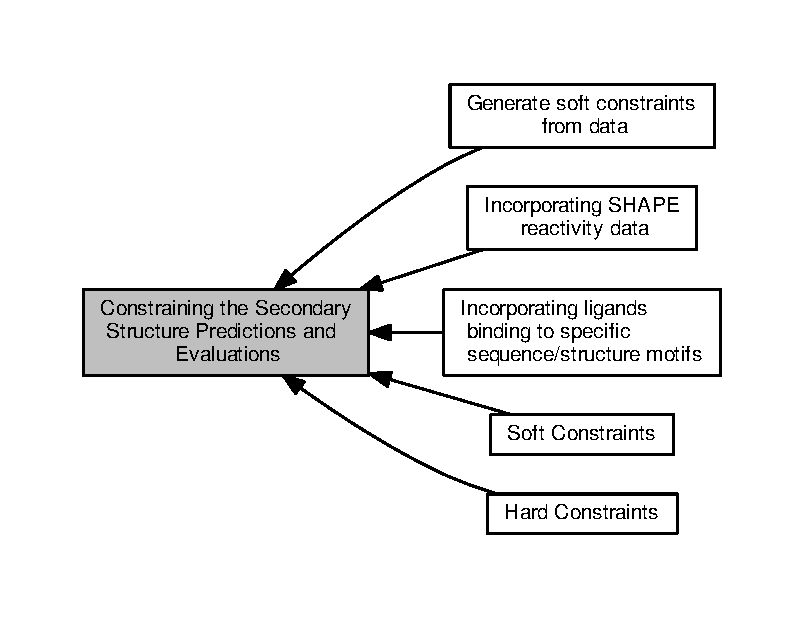
\includegraphics[width=350pt]{group__constraints}
\end{center}
\end{figure}
\subsection*{Modules}
\begin{DoxyCompactItemize}
\item 
\hyperlink{group__hard__constraints}{Hard Constraints}
\begin{DoxyCompactList}\small\item\em This module covers all functionality for hard constraints in secondary structure prediction. \end{DoxyCompactList}\item 
\hyperlink{group__soft__constraints}{Soft Constraints}
\begin{DoxyCompactList}\small\item\em Functions and data structures for secondary structure soft constraints. \end{DoxyCompactList}\item 
\hyperlink{group__SHAPE__reactivities}{Incorporating S\+H\+A\+P\+E reactivity data}
\begin{DoxyCompactList}\small\item\em Incorporate S\+H\+A\+P\+E reactivity structure probing data into the folding recursions by means of soft constraints. \end{DoxyCompactList}\item 
\hyperlink{group__ligands}{Incorporating ligands binding to specific sequence/structure motifs}
\begin{DoxyCompactList}\small\item\em This module covers functions that enable the incorporation of ligand binding free energies to specific hairpin/interior loop motifs by means of generic soft constraints. \end{DoxyCompactList}\item 
\hyperlink{group__perturbation}{Generate soft constraints from data}
\begin{DoxyCompactList}\small\item\em Find a vector of perturbation energies that minimizes the discripancies between predicted and observed pairing probabilities and the amount of neccessary adjustments. \end{DoxyCompactList}\end{DoxyCompactItemize}
\subsection*{Files}
\begin{DoxyCompactItemize}
\item 
file \hyperlink{constraints_8h}{constraints.\+h}
\begin{DoxyCompactList}\small\item\em Functions and data structures for constraining secondary structure predictions and evaluation. \end{DoxyCompactList}\end{DoxyCompactItemize}
\subsection*{Macros}
\begin{DoxyCompactItemize}
\item 
\#define \hyperlink{group__constraints_ga62e0ed0c33002c09423de4e646f85a2b}{V\+R\+N\+A\+\_\+\+C\+O\+N\+S\+T\+R\+A\+I\+N\+T\+\_\+\+F\+I\+L\+E}~0
\begin{DoxyCompactList}\small\item\em Flag for \hyperlink{group__constraints_ga35a401f680969a556858a8dd5f1d07cc}{vrna\+\_\+constraints\+\_\+add()} to indicate that constraints are present in a text file. \end{DoxyCompactList}\item 
\#define \hyperlink{group__constraints_ga62aa195893d02d1a79ca94952748df36}{V\+R\+N\+A\+\_\+\+C\+O\+N\+S\+T\+R\+A\+I\+N\+T\+\_\+\+S\+O\+F\+T\+\_\+\+M\+F\+E}~0
\begin{DoxyCompactList}\small\item\em Indicate generation of constraints for M\+F\+E folding. \end{DoxyCompactList}\item 
\#define \hyperlink{group__constraints_ga03fb5000c19b9a2082bf4ea30a543045}{V\+R\+N\+A\+\_\+\+C\+O\+N\+S\+T\+R\+A\+I\+N\+T\+\_\+\+S\+O\+F\+T\+\_\+\+P\+F}~\hyperlink{group__fold__compound_gabfbadcddda3e74ce7f49035ef8f058f7}{V\+R\+N\+A\+\_\+\+O\+P\+T\+I\+O\+N\+\_\+\+P\+F}
\begin{DoxyCompactList}\small\item\em Indicate generation of constraints for partition function computation. \end{DoxyCompactList}\item 
\#define \hyperlink{group__constraints_ga8bd41ebc8039378d242e4e8c273716a5}{V\+R\+N\+A\+\_\+\+D\+E\+C\+O\+M\+P\+\_\+\+P\+A\+I\+R\+\_\+\+H\+P}~1
\begin{DoxyCompactList}\small\item\em Flag passed to generic softt constraints callback to indicate hairpin loop decomposition step. \end{DoxyCompactList}\item 
\#define \hyperlink{group__constraints_gaeab04f34d7730cff2d651d782f95d857}{V\+R\+N\+A\+\_\+\+D\+E\+C\+O\+M\+P\+\_\+\+P\+A\+I\+R\+\_\+\+I\+L}~2
\begin{DoxyCompactList}\small\item\em Indicator for interior loop decomposition step. \end{DoxyCompactList}\item 
\#define \hyperlink{group__constraints_gaa15b1185673f0b9e900c4748d45f388f}{V\+R\+N\+A\+\_\+\+D\+E\+C\+O\+M\+P\+\_\+\+P\+A\+I\+R\+\_\+\+M\+L}~3
\begin{DoxyCompactList}\small\item\em Indicator for multibranch loop decomposition step. \end{DoxyCompactList}\item 
\#define \hyperlink{group__constraints_ga735517266f2e35e1374b8f1ea77ef23e}{V\+R\+N\+A\+\_\+\+D\+E\+C\+O\+M\+P\+\_\+\+M\+L\+\_\+\+M\+L\+\_\+\+M\+L}~5
\begin{DoxyCompactList}\small\item\em Indicator for decomposition of multibranch loop part. \end{DoxyCompactList}\item 
\#define \hyperlink{group__constraints_ga4a23054c75d8efc785de50e3ea87602f}{V\+R\+N\+A\+\_\+\+D\+E\+C\+O\+M\+P\+\_\+\+M\+L\+\_\+\+S\+T\+E\+M}~4
\begin{DoxyCompactList}\small\item\em Indicator for decomposition of multibranch loop part. \end{DoxyCompactList}\item 
\#define \hyperlink{group__constraints_ga7f4cb9ff7a33e67f0539bd39e7b19a78}{V\+R\+N\+A\+\_\+\+D\+E\+C\+O\+M\+P\+\_\+\+M\+L\+\_\+\+M\+L}~6
\begin{DoxyCompactList}\small\item\em Indicator for decomposition of multibranch loop part. \end{DoxyCompactList}\item 
\#define \hyperlink{group__constraints_gae6478dda14e50e2f2cb9ef333a29256e}{V\+R\+N\+A\+\_\+\+D\+E\+C\+O\+M\+P\+\_\+\+M\+L\+\_\+\+U\+P}~11
\begin{DoxyCompactList}\small\item\em Indicator for decomposition of multibranch loop part. \end{DoxyCompactList}\item 
\#define \hyperlink{group__constraints_ga63d8ceb8c96ae3b463e529e28cc0fe98}{V\+R\+N\+A\+\_\+\+D\+E\+C\+O\+M\+P\+\_\+\+M\+L\+\_\+\+M\+L\+\_\+\+S\+T\+E\+M}~20
\begin{DoxyCompactList}\small\item\em Indicator for decomposition of multibranch loop part. \end{DoxyCompactList}\item 
\#define \hyperlink{group__constraints_ga4fe48d575830b16c208e280e01ab1497}{V\+R\+N\+A\+\_\+\+D\+E\+C\+O\+M\+P\+\_\+\+M\+L\+\_\+\+C\+O\+A\+X\+I\+A\+L}~13
\begin{DoxyCompactList}\small\item\em Indicator for decomposition of multibranch loop part. \end{DoxyCompactList}\item 
\#define \hyperlink{group__constraints_ga437adf5115c1999304eff26b41e4c9b6}{V\+R\+N\+A\+\_\+\+D\+E\+C\+O\+M\+P\+\_\+\+E\+X\+T\+\_\+\+E\+X\+T}~9
\begin{DoxyCompactList}\small\item\em Indicator for decomposition of exterior loop part. \end{DoxyCompactList}\item 
\#define \hyperlink{group__constraints_gaff1ddaffe86d984623910b40cc8a8717}{V\+R\+N\+A\+\_\+\+D\+E\+C\+O\+M\+P\+\_\+\+E\+X\+T\+\_\+\+U\+P}~8
\begin{DoxyCompactList}\small\item\em Indicator for decomposition of exterior loop part. \end{DoxyCompactList}\item 
\#define \hyperlink{group__constraints_gae44b5ace0d9b4a29088069ecb4cec441}{V\+R\+N\+A\+\_\+\+D\+E\+C\+O\+M\+P\+\_\+\+E\+X\+T\+\_\+\+S\+T\+E\+M}~14
\begin{DoxyCompactList}\small\item\em Indicator for decomposition of exterior loop part. \end{DoxyCompactList}\item 
\#define \hyperlink{group__constraints_ga803bd818b3f4b2b0a4a5cfa2f7dc2045}{V\+R\+N\+A\+\_\+\+D\+E\+C\+O\+M\+P\+\_\+\+E\+X\+T\+\_\+\+E\+X\+T\+\_\+\+E\+X\+T}~15
\begin{DoxyCompactList}\small\item\em Indicator for decomposition of exterior loop part. \end{DoxyCompactList}\item 
\#define \hyperlink{group__constraints_gabb09c5b78b75a44502fc77b950125c1e}{V\+R\+N\+A\+\_\+\+D\+E\+C\+O\+M\+P\+\_\+\+E\+X\+T\+\_\+\+S\+T\+E\+M\+\_\+\+E\+X\+T}~16
\begin{DoxyCompactList}\small\item\em Indicator for decomposition of exterior loop part. \end{DoxyCompactList}\item 
\hypertarget{group__constraints_gae7554cd3ff089360c02e4920229e221c}{}\#define \hyperlink{group__constraints_gae7554cd3ff089360c02e4920229e221c}{V\+R\+N\+A\+\_\+\+D\+E\+C\+O\+M\+P\+\_\+\+E\+X\+T\+\_\+\+S\+T\+E\+M\+\_\+\+O\+U\+T\+S\+I\+D\+E}~17\label{group__constraints_gae7554cd3ff089360c02e4920229e221c}

\begin{DoxyCompactList}\small\item\em Indicator for decomposition of exterior loop part. \end{DoxyCompactList}\item 
\#define \hyperlink{group__constraints_ga06efd054c9271438f6d82d4559d9e69f}{V\+R\+N\+A\+\_\+\+D\+E\+C\+O\+M\+P\+\_\+\+E\+X\+T\+\_\+\+E\+X\+T\+\_\+\+S\+T\+E\+M}~18
\begin{DoxyCompactList}\small\item\em Indicator for decomposition of exterior loop part. \end{DoxyCompactList}\item 
\#define \hyperlink{group__constraints_ga2e75d7a77118735b32f25422d9686719}{V\+R\+N\+A\+\_\+\+D\+E\+C\+O\+M\+P\+\_\+\+E\+X\+T\+\_\+\+E\+X\+T\+\_\+\+S\+T\+E\+M1}~19
\begin{DoxyCompactList}\small\item\em Indicator for decomposition of exterior loop part. \end{DoxyCompactList}\end{DoxyCompactItemize}
\subsection*{Functions}
\begin{DoxyCompactItemize}
\item 
void \hyperlink{group__constraints_ga35a401f680969a556858a8dd5f1d07cc}{vrna\+\_\+constraints\+\_\+add} (\hyperlink{group__fold__compound_ga1b0cef17fd40466cef5968eaeeff6166}{vrna\+\_\+fold\+\_\+compound\+\_\+t} $\ast$vc, const char $\ast$constraint, unsigned int options)
\begin{DoxyCompactList}\small\item\em Add constraints to a \hyperlink{group__fold__compound_ga1b0cef17fd40466cef5968eaeeff6166}{vrna\+\_\+fold\+\_\+compound\+\_\+t} data structure. \end{DoxyCompactList}\item 
void \hyperlink{group__constraints_gaa1f20b53bf09ac2e6b0dbb13f7d89670}{vrna\+\_\+message\+\_\+constraint\+\_\+options} (unsigned int option)
\begin{DoxyCompactList}\small\item\em Print a help message for pseudo dot-\/bracket structure constraint characters to stdout. (constraint support is specified by option parameter) \end{DoxyCompactList}\item 
void \hyperlink{group__constraints_gaec7e13fa0465c2acc7a621d1aecb709f}{vrna\+\_\+message\+\_\+constraint\+\_\+options\+\_\+all} (void)
\begin{DoxyCompactList}\small\item\em Print structure constraint characters to stdout (full constraint support) \end{DoxyCompactList}\end{DoxyCompactItemize}


\subsection{Detailed Description}
This module covers all functions and variables related to the problem of incorporating secondary structure constraints into the folding recursions. 

This module provides general functions that allow for an easy control of constrained secondary structure prediction and evaluation. Secondary Structure constraints can be subdivided into two groups\+:


\begin{DoxyItemize}
\item \hyperlink{group__hard__constraints}{Hard Constraints}, and
\item \hyperlink{group__soft__constraints}{Soft Constraints}.
\end{DoxyItemize}

While Hard-\/\+Constraints directly influence the production rules used in the folding recursions by allowing, disallowing, or enforcing certain decomposition steps, Soft-\/constraints on the other hand are used to change position specific contributions in the recursions by adding bonuses/penalties in form of pseudo free energies to certain loop configurations.

Secondary structure constraints are always applied at decomposition level, i.\+e. in each step of the recursive structure decomposition, for instance during M\+F\+E prediction. Below is a visualization of the decomposition scheme

 
\begin{DoxyImageNoCaption}
  \mbox{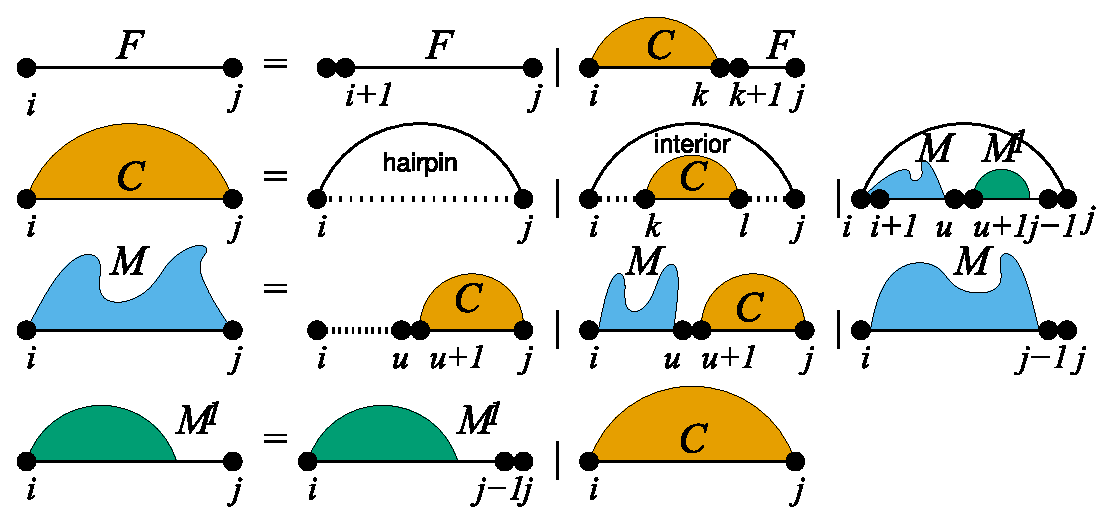
\includegraphics[width=\textwidth,height=\textheight/2,keepaspectratio=true]{recursions}}
\end{DoxyImageNoCaption}


For \hyperlink{group__hard__constraints}{Hard Constraints} the following option flags may be used to constrain the pairing behavior of single, or pairs of nucleotides\+:


\begin{DoxyItemize}
\item \hyperlink{group__hard__constraints_ga9418eda62a5dec070896702c279d2548}{V\+R\+N\+A\+\_\+\+C\+O\+N\+S\+T\+R\+A\+I\+N\+T\+\_\+\+C\+O\+N\+T\+E\+X\+T\+\_\+\+E\+X\+T\+\_\+\+L\+O\+O\+P} -\/ Hard constraints flag, base pair in the exterior loop.
\item \hyperlink{group__hard__constraints_ga79203702b197b6b9d3b78eed40663eb1}{V\+R\+N\+A\+\_\+\+C\+O\+N\+S\+T\+R\+A\+I\+N\+T\+\_\+\+C\+O\+N\+T\+E\+X\+T\+\_\+\+H\+P\+\_\+\+L\+O\+O\+P} -\/ Hard constraints flag, base pair encloses hairpin loop.
\item \hyperlink{group__hard__constraints_ga21feeab3a9e5fa5a9e3d9ac0fcf5994f}{V\+R\+N\+A\+\_\+\+C\+O\+N\+S\+T\+R\+A\+I\+N\+T\+\_\+\+C\+O\+N\+T\+E\+X\+T\+\_\+\+I\+N\+T\+\_\+\+L\+O\+O\+P} -\/ Hard constraints flag, base pair encloses an interior loop.
\item \hyperlink{group__hard__constraints_ga0536288e04ff6332ecdc23ca4705402b}{V\+R\+N\+A\+\_\+\+C\+O\+N\+S\+T\+R\+A\+I\+N\+T\+\_\+\+C\+O\+N\+T\+E\+X\+T\+\_\+\+I\+N\+T\+\_\+\+L\+O\+O\+P\+\_\+\+E\+N\+C} -\/ Hard constraints flag, base pair encloses a multi branch loop.
\item \hyperlink{group__hard__constraints_ga456ecd2ff00056bb64da8dd4f61bbfc5}{V\+R\+N\+A\+\_\+\+C\+O\+N\+S\+T\+R\+A\+I\+N\+T\+\_\+\+C\+O\+N\+T\+E\+X\+T\+\_\+\+M\+B\+\_\+\+L\+O\+O\+P} -\/ Hard constraints flag, base pair is enclosed in an interior loop.
\item \hyperlink{group__hard__constraints_ga02a3d703ddbcfce393e4bbfcb9db7077}{V\+R\+N\+A\+\_\+\+C\+O\+N\+S\+T\+R\+A\+I\+N\+T\+\_\+\+C\+O\+N\+T\+E\+X\+T\+\_\+\+M\+B\+\_\+\+L\+O\+O\+P\+\_\+\+E\+N\+C} -\/ Hard constraints flag, base pair is enclosed in a multi branch loop.
\item \#\+V\+R\+N\+A\+\_\+\+C\+O\+N\+S\+T\+R\+A\+I\+N\+T\+\_\+\+C\+O\+N\+T\+E\+X\+T\+\_\+\+E\+N\+F\+O\+R\+C\+E -\/
\item \#\+V\+R\+N\+A\+\_\+\+C\+O\+N\+S\+T\+R\+A\+I\+N\+T\+\_\+\+C\+O\+N\+T\+E\+X\+T\+\_\+\+N\+O\+\_\+\+R\+E\+M\+O\+V\+E -\/
\item \hyperlink{group__hard__constraints_ga886d9127c49bb982a4b67cd7581e8a5a}{V\+R\+N\+A\+\_\+\+C\+O\+N\+S\+T\+R\+A\+I\+N\+T\+\_\+\+C\+O\+N\+T\+E\+X\+T\+\_\+\+A\+L\+L\+\_\+\+L\+O\+O\+P\+S} -\/ Hard constraints flag, shortcut for all base pairs.
\end{DoxyItemize}

However, for \hyperlink{group__soft__constraints}{Soft Constraints} we do not allow for simple loop type dependent constraining. But soft constraints are equipped with generic constraint support. This enables the user to pass arbitrary callback functions that return auxiliary energy contributions for evaluation the avaluation of any decomposition.

The callback will then always be notified about the type of decomposition that is happening, and the corresponding delimiting sequence positions. The following decomposition steps are distinguished, and should be captured by the user\textquotesingle{}s implementation of the callback\+:


\begin{DoxyItemize}
\item \hyperlink{group__constraints_ga8bd41ebc8039378d242e4e8c273716a5}{V\+R\+N\+A\+\_\+\+D\+E\+C\+O\+M\+P\+\_\+\+P\+A\+I\+R\+\_\+\+H\+P} -\/ Flag passed to generic softt constraints callback to indicate hairpin loop decomposition step.
\item \hyperlink{group__constraints_gaeab04f34d7730cff2d651d782f95d857}{V\+R\+N\+A\+\_\+\+D\+E\+C\+O\+M\+P\+\_\+\+P\+A\+I\+R\+\_\+\+I\+L} -\/ Indicator for interior loop decomposition step.
\item \hyperlink{group__constraints_gaa15b1185673f0b9e900c4748d45f388f}{V\+R\+N\+A\+\_\+\+D\+E\+C\+O\+M\+P\+\_\+\+P\+A\+I\+R\+\_\+\+M\+L} -\/ Indicator for multibranch loop decomposition step.
\item \hyperlink{group__constraints_ga735517266f2e35e1374b8f1ea77ef23e}{V\+R\+N\+A\+\_\+\+D\+E\+C\+O\+M\+P\+\_\+\+M\+L\+\_\+\+M\+L\+\_\+\+M\+L} -\/ Indicator for decomposition of multibranch loop part.
\item \hyperlink{group__constraints_ga4a23054c75d8efc785de50e3ea87602f}{V\+R\+N\+A\+\_\+\+D\+E\+C\+O\+M\+P\+\_\+\+M\+L\+\_\+\+S\+T\+E\+M} -\/ Indicator for decomposition of multibranch loop part.
\item \hyperlink{group__constraints_ga7f4cb9ff7a33e67f0539bd39e7b19a78}{V\+R\+N\+A\+\_\+\+D\+E\+C\+O\+M\+P\+\_\+\+M\+L\+\_\+\+M\+L} -\/ Indicator for decomposition of multibranch loop part.
\item \hyperlink{group__constraints_gae6478dda14e50e2f2cb9ef333a29256e}{V\+R\+N\+A\+\_\+\+D\+E\+C\+O\+M\+P\+\_\+\+M\+L\+\_\+\+U\+P} -\/ Indicator for decomposition of multibranch loop part.
\item \hyperlink{group__constraints_ga63d8ceb8c96ae3b463e529e28cc0fe98}{V\+R\+N\+A\+\_\+\+D\+E\+C\+O\+M\+P\+\_\+\+M\+L\+\_\+\+M\+L\+\_\+\+S\+T\+E\+M} -\/ Indicator for decomposition of multibranch loop part.
\item \hyperlink{group__constraints_ga4fe48d575830b16c208e280e01ab1497}{V\+R\+N\+A\+\_\+\+D\+E\+C\+O\+M\+P\+\_\+\+M\+L\+\_\+\+C\+O\+A\+X\+I\+A\+L} -\/ Indicator for decomposition of multibranch loop part.
\item \hyperlink{group__constraints_ga437adf5115c1999304eff26b41e4c9b6}{V\+R\+N\+A\+\_\+\+D\+E\+C\+O\+M\+P\+\_\+\+E\+X\+T\+\_\+\+E\+X\+T} -\/ Indicator for decomposition of exterior loop part.
\item \hyperlink{group__constraints_gaff1ddaffe86d984623910b40cc8a8717}{V\+R\+N\+A\+\_\+\+D\+E\+C\+O\+M\+P\+\_\+\+E\+X\+T\+\_\+\+U\+P} -\/ Indicator for decomposition of exterior loop part.
\item \hyperlink{group__constraints_gae44b5ace0d9b4a29088069ecb4cec441}{V\+R\+N\+A\+\_\+\+D\+E\+C\+O\+M\+P\+\_\+\+E\+X\+T\+\_\+\+S\+T\+E\+M} -\/ Indicator for decomposition of exterior loop part.
\item \hyperlink{group__constraints_ga803bd818b3f4b2b0a4a5cfa2f7dc2045}{V\+R\+N\+A\+\_\+\+D\+E\+C\+O\+M\+P\+\_\+\+E\+X\+T\+\_\+\+E\+X\+T\+\_\+\+E\+X\+T} -\/ Indicator for decomposition of exterior loop part.
\item \hyperlink{group__constraints_gabb09c5b78b75a44502fc77b950125c1e}{V\+R\+N\+A\+\_\+\+D\+E\+C\+O\+M\+P\+\_\+\+E\+X\+T\+\_\+\+S\+T\+E\+M\+\_\+\+E\+X\+T} -\/ Indicator for decomposition of exterior loop part.
\item \hyperlink{group__constraints_gae7554cd3ff089360c02e4920229e221c}{V\+R\+N\+A\+\_\+\+D\+E\+C\+O\+M\+P\+\_\+\+E\+X\+T\+\_\+\+S\+T\+E\+M\+\_\+\+O\+U\+T\+S\+I\+D\+E} -\/ Indicator for decomposition of exterior loop part.
\item \hyperlink{group__constraints_ga06efd054c9271438f6d82d4559d9e69f}{V\+R\+N\+A\+\_\+\+D\+E\+C\+O\+M\+P\+\_\+\+E\+X\+T\+\_\+\+E\+X\+T\+\_\+\+S\+T\+E\+M} -\/ Indicator for decomposition of exterior loop part.
\item \hyperlink{group__constraints_ga2e75d7a77118735b32f25422d9686719}{V\+R\+N\+A\+\_\+\+D\+E\+C\+O\+M\+P\+\_\+\+E\+X\+T\+\_\+\+E\+X\+T\+\_\+\+S\+T\+E\+M1} -\/ Indicator for decomposition of exterior loop part.
\end{DoxyItemize}

Simplified interfaces to the soft constraints framework can be obtained by the implementations in the submodules


\begin{DoxyItemize}
\item \hyperlink{group__SHAPE__reactivities}{Incorporating S\+H\+A\+P\+E reactivity data} and
\item \hyperlink{group__ligands}{Incorporating ligands binding to specific sequence/structure motifs}.
\end{DoxyItemize}

An implementation that generates soft constraints for unpaired nucleotides by minimizing the discrepancy between their predicted and expected pairing probability is available in submodule \hyperlink{group__perturbation}{Generate soft constraints from data}. 

\subsection{Macro Definition Documentation}
\hypertarget{group__constraints_ga62e0ed0c33002c09423de4e646f85a2b}{}\index{Constraining the Secondary Structure Predictions and Evaluations@{Constraining the Secondary Structure Predictions and Evaluations}!V\+R\+N\+A\+\_\+\+C\+O\+N\+S\+T\+R\+A\+I\+N\+T\+\_\+\+F\+I\+L\+E@{V\+R\+N\+A\+\_\+\+C\+O\+N\+S\+T\+R\+A\+I\+N\+T\+\_\+\+F\+I\+L\+E}}
\index{V\+R\+N\+A\+\_\+\+C\+O\+N\+S\+T\+R\+A\+I\+N\+T\+\_\+\+F\+I\+L\+E@{V\+R\+N\+A\+\_\+\+C\+O\+N\+S\+T\+R\+A\+I\+N\+T\+\_\+\+F\+I\+L\+E}!Constraining the Secondary Structure Predictions and Evaluations@{Constraining the Secondary Structure Predictions and Evaluations}}
\subsubsection[{V\+R\+N\+A\+\_\+\+C\+O\+N\+S\+T\+R\+A\+I\+N\+T\+\_\+\+F\+I\+L\+E}]{\setlength{\rightskip}{0pt plus 5cm}\#define V\+R\+N\+A\+\_\+\+C\+O\+N\+S\+T\+R\+A\+I\+N\+T\+\_\+\+F\+I\+L\+E~0}\label{group__constraints_ga62e0ed0c33002c09423de4e646f85a2b}


{\ttfamily \#include $<$\hyperlink{constraints_8h}{Vienna\+R\+N\+A/constraints.\+h}$>$}



Flag for \hyperlink{group__constraints_ga35a401f680969a556858a8dd5f1d07cc}{vrna\+\_\+constraints\+\_\+add()} to indicate that constraints are present in a text file. 

\begin{DoxySeeAlso}{See also}
\hyperlink{group__constraints_ga35a401f680969a556858a8dd5f1d07cc}{vrna\+\_\+constraints\+\_\+add()} 
\end{DoxySeeAlso}
\begin{DoxyRefDesc}{Deprecated}
\item[\hyperlink{deprecated__deprecated000039}{Deprecated}]Use 0 instead!\end{DoxyRefDesc}
\hypertarget{group__constraints_ga62aa195893d02d1a79ca94952748df36}{}\index{Constraining the Secondary Structure Predictions and Evaluations@{Constraining the Secondary Structure Predictions and Evaluations}!V\+R\+N\+A\+\_\+\+C\+O\+N\+S\+T\+R\+A\+I\+N\+T\+\_\+\+S\+O\+F\+T\+\_\+\+M\+F\+E@{V\+R\+N\+A\+\_\+\+C\+O\+N\+S\+T\+R\+A\+I\+N\+T\+\_\+\+S\+O\+F\+T\+\_\+\+M\+F\+E}}
\index{V\+R\+N\+A\+\_\+\+C\+O\+N\+S\+T\+R\+A\+I\+N\+T\+\_\+\+S\+O\+F\+T\+\_\+\+M\+F\+E@{V\+R\+N\+A\+\_\+\+C\+O\+N\+S\+T\+R\+A\+I\+N\+T\+\_\+\+S\+O\+F\+T\+\_\+\+M\+F\+E}!Constraining the Secondary Structure Predictions and Evaluations@{Constraining the Secondary Structure Predictions and Evaluations}}
\subsubsection[{V\+R\+N\+A\+\_\+\+C\+O\+N\+S\+T\+R\+A\+I\+N\+T\+\_\+\+S\+O\+F\+T\+\_\+\+M\+F\+E}]{\setlength{\rightskip}{0pt plus 5cm}\#define V\+R\+N\+A\+\_\+\+C\+O\+N\+S\+T\+R\+A\+I\+N\+T\+\_\+\+S\+O\+F\+T\+\_\+\+M\+F\+E~0}\label{group__constraints_ga62aa195893d02d1a79ca94952748df36}


{\ttfamily \#include $<$\hyperlink{constraints_8h}{Vienna\+R\+N\+A/constraints.\+h}$>$}



Indicate generation of constraints for M\+F\+E folding. 

\begin{DoxyRefDesc}{Deprecated}
\item[\hyperlink{deprecated__deprecated000040}{Deprecated}]This flag has no meaning anymore, since constraints are now always stored!\end{DoxyRefDesc}
\hypertarget{group__constraints_ga03fb5000c19b9a2082bf4ea30a543045}{}\index{Constraining the Secondary Structure Predictions and Evaluations@{Constraining the Secondary Structure Predictions and Evaluations}!V\+R\+N\+A\+\_\+\+C\+O\+N\+S\+T\+R\+A\+I\+N\+T\+\_\+\+S\+O\+F\+T\+\_\+\+P\+F@{V\+R\+N\+A\+\_\+\+C\+O\+N\+S\+T\+R\+A\+I\+N\+T\+\_\+\+S\+O\+F\+T\+\_\+\+P\+F}}
\index{V\+R\+N\+A\+\_\+\+C\+O\+N\+S\+T\+R\+A\+I\+N\+T\+\_\+\+S\+O\+F\+T\+\_\+\+P\+F@{V\+R\+N\+A\+\_\+\+C\+O\+N\+S\+T\+R\+A\+I\+N\+T\+\_\+\+S\+O\+F\+T\+\_\+\+P\+F}!Constraining the Secondary Structure Predictions and Evaluations@{Constraining the Secondary Structure Predictions and Evaluations}}
\subsubsection[{V\+R\+N\+A\+\_\+\+C\+O\+N\+S\+T\+R\+A\+I\+N\+T\+\_\+\+S\+O\+F\+T\+\_\+\+P\+F}]{\setlength{\rightskip}{0pt plus 5cm}\#define V\+R\+N\+A\+\_\+\+C\+O\+N\+S\+T\+R\+A\+I\+N\+T\+\_\+\+S\+O\+F\+T\+\_\+\+P\+F~{\bf V\+R\+N\+A\+\_\+\+O\+P\+T\+I\+O\+N\+\_\+\+P\+F}}\label{group__constraints_ga03fb5000c19b9a2082bf4ea30a543045}


{\ttfamily \#include $<$\hyperlink{constraints_8h}{Vienna\+R\+N\+A/constraints.\+h}$>$}



Indicate generation of constraints for partition function computation. 

\begin{DoxyRefDesc}{Deprecated}
\item[\hyperlink{deprecated__deprecated000041}{Deprecated}]Use \hyperlink{group__fold__compound_gabfbadcddda3e74ce7f49035ef8f058f7}{V\+R\+N\+A\+\_\+\+O\+P\+T\+I\+O\+N\+\_\+\+P\+F} instead!\end{DoxyRefDesc}
\hypertarget{group__constraints_ga8bd41ebc8039378d242e4e8c273716a5}{}\index{Constraining the Secondary Structure Predictions and Evaluations@{Constraining the Secondary Structure Predictions and Evaluations}!V\+R\+N\+A\+\_\+\+D\+E\+C\+O\+M\+P\+\_\+\+P\+A\+I\+R\+\_\+\+H\+P@{V\+R\+N\+A\+\_\+\+D\+E\+C\+O\+M\+P\+\_\+\+P\+A\+I\+R\+\_\+\+H\+P}}
\index{V\+R\+N\+A\+\_\+\+D\+E\+C\+O\+M\+P\+\_\+\+P\+A\+I\+R\+\_\+\+H\+P@{V\+R\+N\+A\+\_\+\+D\+E\+C\+O\+M\+P\+\_\+\+P\+A\+I\+R\+\_\+\+H\+P}!Constraining the Secondary Structure Predictions and Evaluations@{Constraining the Secondary Structure Predictions and Evaluations}}
\subsubsection[{V\+R\+N\+A\+\_\+\+D\+E\+C\+O\+M\+P\+\_\+\+P\+A\+I\+R\+\_\+\+H\+P}]{\setlength{\rightskip}{0pt plus 5cm}\#define V\+R\+N\+A\+\_\+\+D\+E\+C\+O\+M\+P\+\_\+\+P\+A\+I\+R\+\_\+\+H\+P~1}\label{group__constraints_ga8bd41ebc8039378d242e4e8c273716a5}


{\ttfamily \#include $<$\hyperlink{constraints_8h}{Vienna\+R\+N\+A/constraints.\+h}$>$}



Flag passed to generic softt constraints callback to indicate hairpin loop decomposition step. 

This flag notifies the soft or hard constraint callback function that the current decomposition step evaluates a hairpin loop enclosed by the base pair $(i,j)$.

 
\begin{DoxyImageNoCaption}
  \mbox{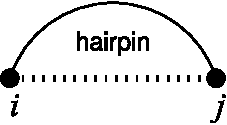
\includegraphics[width=\textwidth,height=\textheight/2,keepaspectratio=true]{decomp_hp}}
\end{DoxyImageNoCaption}
 \hypertarget{group__constraints_gaeab04f34d7730cff2d651d782f95d857}{}\index{Constraining the Secondary Structure Predictions and Evaluations@{Constraining the Secondary Structure Predictions and Evaluations}!V\+R\+N\+A\+\_\+\+D\+E\+C\+O\+M\+P\+\_\+\+P\+A\+I\+R\+\_\+\+I\+L@{V\+R\+N\+A\+\_\+\+D\+E\+C\+O\+M\+P\+\_\+\+P\+A\+I\+R\+\_\+\+I\+L}}
\index{V\+R\+N\+A\+\_\+\+D\+E\+C\+O\+M\+P\+\_\+\+P\+A\+I\+R\+\_\+\+I\+L@{V\+R\+N\+A\+\_\+\+D\+E\+C\+O\+M\+P\+\_\+\+P\+A\+I\+R\+\_\+\+I\+L}!Constraining the Secondary Structure Predictions and Evaluations@{Constraining the Secondary Structure Predictions and Evaluations}}
\subsubsection[{V\+R\+N\+A\+\_\+\+D\+E\+C\+O\+M\+P\+\_\+\+P\+A\+I\+R\+\_\+\+I\+L}]{\setlength{\rightskip}{0pt plus 5cm}\#define V\+R\+N\+A\+\_\+\+D\+E\+C\+O\+M\+P\+\_\+\+P\+A\+I\+R\+\_\+\+I\+L~2}\label{group__constraints_gaeab04f34d7730cff2d651d782f95d857}


{\ttfamily \#include $<$\hyperlink{constraints_8h}{Vienna\+R\+N\+A/constraints.\+h}$>$}



Indicator for interior loop decomposition step. 

This flag notifies the soft or hard constraint callback function that the current decomposition step evaluates an interior loop enclosed by the base pair $(i,j)$, and enclosing the base pair $(k,l)$.

 
\begin{DoxyImageNoCaption}
  \mbox{
\includegraphics[width=\textwidth,height=\textheight/2,keepaspectratio=true]{decomp_il}}
\end{DoxyImageNoCaption}
 \hypertarget{group__constraints_gaa15b1185673f0b9e900c4748d45f388f}{}\index{Constraining the Secondary Structure Predictions and Evaluations@{Constraining the Secondary Structure Predictions and Evaluations}!V\+R\+N\+A\+\_\+\+D\+E\+C\+O\+M\+P\+\_\+\+P\+A\+I\+R\+\_\+\+M\+L@{V\+R\+N\+A\+\_\+\+D\+E\+C\+O\+M\+P\+\_\+\+P\+A\+I\+R\+\_\+\+M\+L}}
\index{V\+R\+N\+A\+\_\+\+D\+E\+C\+O\+M\+P\+\_\+\+P\+A\+I\+R\+\_\+\+M\+L@{V\+R\+N\+A\+\_\+\+D\+E\+C\+O\+M\+P\+\_\+\+P\+A\+I\+R\+\_\+\+M\+L}!Constraining the Secondary Structure Predictions and Evaluations@{Constraining the Secondary Structure Predictions and Evaluations}}
\subsubsection[{V\+R\+N\+A\+\_\+\+D\+E\+C\+O\+M\+P\+\_\+\+P\+A\+I\+R\+\_\+\+M\+L}]{\setlength{\rightskip}{0pt plus 5cm}\#define V\+R\+N\+A\+\_\+\+D\+E\+C\+O\+M\+P\+\_\+\+P\+A\+I\+R\+\_\+\+M\+L~3}\label{group__constraints_gaa15b1185673f0b9e900c4748d45f388f}


{\ttfamily \#include $<$\hyperlink{constraints_8h}{Vienna\+R\+N\+A/constraints.\+h}$>$}



Indicator for multibranch loop decomposition step. 

This flag notifies the soft or hard constraint callback function that the current decomposition step evaluates a multibranch loop enclosed by the base pair $(i,j)$, and consisting of some enclosed multi loop content from k to l.

 
\begin{DoxyImageNoCaption}
  \mbox{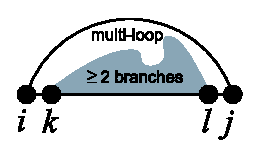
\includegraphics[width=\textwidth,height=\textheight/2,keepaspectratio=true]{decomp_ml}}
\end{DoxyImageNoCaption}
 \hypertarget{group__constraints_ga735517266f2e35e1374b8f1ea77ef23e}{}\index{Constraining the Secondary Structure Predictions and Evaluations@{Constraining the Secondary Structure Predictions and Evaluations}!V\+R\+N\+A\+\_\+\+D\+E\+C\+O\+M\+P\+\_\+\+M\+L\+\_\+\+M\+L\+\_\+\+M\+L@{V\+R\+N\+A\+\_\+\+D\+E\+C\+O\+M\+P\+\_\+\+M\+L\+\_\+\+M\+L\+\_\+\+M\+L}}
\index{V\+R\+N\+A\+\_\+\+D\+E\+C\+O\+M\+P\+\_\+\+M\+L\+\_\+\+M\+L\+\_\+\+M\+L@{V\+R\+N\+A\+\_\+\+D\+E\+C\+O\+M\+P\+\_\+\+M\+L\+\_\+\+M\+L\+\_\+\+M\+L}!Constraining the Secondary Structure Predictions and Evaluations@{Constraining the Secondary Structure Predictions and Evaluations}}
\subsubsection[{V\+R\+N\+A\+\_\+\+D\+E\+C\+O\+M\+P\+\_\+\+M\+L\+\_\+\+M\+L\+\_\+\+M\+L}]{\setlength{\rightskip}{0pt plus 5cm}\#define V\+R\+N\+A\+\_\+\+D\+E\+C\+O\+M\+P\+\_\+\+M\+L\+\_\+\+M\+L\+\_\+\+M\+L~5}\label{group__constraints_ga735517266f2e35e1374b8f1ea77ef23e}


{\ttfamily \#include $<$\hyperlink{constraints_8h}{Vienna\+R\+N\+A/constraints.\+h}$>$}



Indicator for decomposition of multibranch loop part. 

This flag notifies the soft or hard constraint callback function that the current decomposition step evaluates a multibranch loop part in the interval $[i:j]$, which will be decomposed into two multibranch loop parts $[i:k]$, and $[l:j]$.

 
\begin{DoxyImageNoCaption}
  \mbox{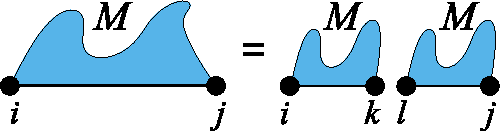
\includegraphics[width=\textwidth,height=\textheight/2,keepaspectratio=true]{decomp_ml_ml_ml}}
\end{DoxyImageNoCaption}
 \hypertarget{group__constraints_ga4a23054c75d8efc785de50e3ea87602f}{}\index{Constraining the Secondary Structure Predictions and Evaluations@{Constraining the Secondary Structure Predictions and Evaluations}!V\+R\+N\+A\+\_\+\+D\+E\+C\+O\+M\+P\+\_\+\+M\+L\+\_\+\+S\+T\+E\+M@{V\+R\+N\+A\+\_\+\+D\+E\+C\+O\+M\+P\+\_\+\+M\+L\+\_\+\+S\+T\+E\+M}}
\index{V\+R\+N\+A\+\_\+\+D\+E\+C\+O\+M\+P\+\_\+\+M\+L\+\_\+\+S\+T\+E\+M@{V\+R\+N\+A\+\_\+\+D\+E\+C\+O\+M\+P\+\_\+\+M\+L\+\_\+\+S\+T\+E\+M}!Constraining the Secondary Structure Predictions and Evaluations@{Constraining the Secondary Structure Predictions and Evaluations}}
\subsubsection[{V\+R\+N\+A\+\_\+\+D\+E\+C\+O\+M\+P\+\_\+\+M\+L\+\_\+\+S\+T\+E\+M}]{\setlength{\rightskip}{0pt plus 5cm}\#define V\+R\+N\+A\+\_\+\+D\+E\+C\+O\+M\+P\+\_\+\+M\+L\+\_\+\+S\+T\+E\+M~4}\label{group__constraints_ga4a23054c75d8efc785de50e3ea87602f}


{\ttfamily \#include $<$\hyperlink{constraints_8h}{Vienna\+R\+N\+A/constraints.\+h}$>$}



Indicator for decomposition of multibranch loop part. 

This flag notifies the soft or hard constraint callback function that the current decomposition step evaluates a multibranch loop part in the interval $[i:j]$, which will be considered a single stem branching off with base pair $(k,l)$.

 
\begin{DoxyImageNoCaption}
  \mbox{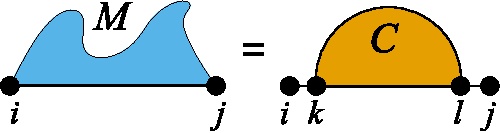
\includegraphics[width=\textwidth,height=\textheight/2,keepaspectratio=true]{decomp_ml_stem}}
\end{DoxyImageNoCaption}
 \hypertarget{group__constraints_ga7f4cb9ff7a33e67f0539bd39e7b19a78}{}\index{Constraining the Secondary Structure Predictions and Evaluations@{Constraining the Secondary Structure Predictions and Evaluations}!V\+R\+N\+A\+\_\+\+D\+E\+C\+O\+M\+P\+\_\+\+M\+L\+\_\+\+M\+L@{V\+R\+N\+A\+\_\+\+D\+E\+C\+O\+M\+P\+\_\+\+M\+L\+\_\+\+M\+L}}
\index{V\+R\+N\+A\+\_\+\+D\+E\+C\+O\+M\+P\+\_\+\+M\+L\+\_\+\+M\+L@{V\+R\+N\+A\+\_\+\+D\+E\+C\+O\+M\+P\+\_\+\+M\+L\+\_\+\+M\+L}!Constraining the Secondary Structure Predictions and Evaluations@{Constraining the Secondary Structure Predictions and Evaluations}}
\subsubsection[{V\+R\+N\+A\+\_\+\+D\+E\+C\+O\+M\+P\+\_\+\+M\+L\+\_\+\+M\+L}]{\setlength{\rightskip}{0pt plus 5cm}\#define V\+R\+N\+A\+\_\+\+D\+E\+C\+O\+M\+P\+\_\+\+M\+L\+\_\+\+M\+L~6}\label{group__constraints_ga7f4cb9ff7a33e67f0539bd39e7b19a78}


{\ttfamily \#include $<$\hyperlink{constraints_8h}{Vienna\+R\+N\+A/constraints.\+h}$>$}



Indicator for decomposition of multibranch loop part. 

This flag notifies the soft or hard constraint callback function that the current decomposition step evaluates a multibranch loop part in the interval $[i:j]$, which will be decomposed into a (usually) smaller multibranch loop part $[k:l]$.

 
\begin{DoxyImageNoCaption}
  \mbox{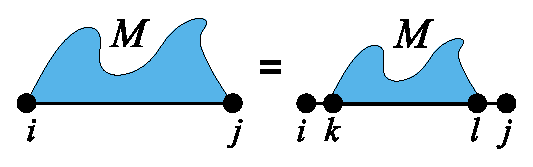
\includegraphics[width=\textwidth,height=\textheight/2,keepaspectratio=true]{decomp_ml_ml}}
\end{DoxyImageNoCaption}
 \hypertarget{group__constraints_gae6478dda14e50e2f2cb9ef333a29256e}{}\index{Constraining the Secondary Structure Predictions and Evaluations@{Constraining the Secondary Structure Predictions and Evaluations}!V\+R\+N\+A\+\_\+\+D\+E\+C\+O\+M\+P\+\_\+\+M\+L\+\_\+\+U\+P@{V\+R\+N\+A\+\_\+\+D\+E\+C\+O\+M\+P\+\_\+\+M\+L\+\_\+\+U\+P}}
\index{V\+R\+N\+A\+\_\+\+D\+E\+C\+O\+M\+P\+\_\+\+M\+L\+\_\+\+U\+P@{V\+R\+N\+A\+\_\+\+D\+E\+C\+O\+M\+P\+\_\+\+M\+L\+\_\+\+U\+P}!Constraining the Secondary Structure Predictions and Evaluations@{Constraining the Secondary Structure Predictions and Evaluations}}
\subsubsection[{V\+R\+N\+A\+\_\+\+D\+E\+C\+O\+M\+P\+\_\+\+M\+L\+\_\+\+U\+P}]{\setlength{\rightskip}{0pt plus 5cm}\#define V\+R\+N\+A\+\_\+\+D\+E\+C\+O\+M\+P\+\_\+\+M\+L\+\_\+\+U\+P~11}\label{group__constraints_gae6478dda14e50e2f2cb9ef333a29256e}


{\ttfamily \#include $<$\hyperlink{constraints_8h}{Vienna\+R\+N\+A/constraints.\+h}$>$}



Indicator for decomposition of multibranch loop part. 

This flag notifies the soft or hard constraint callback function that the current decomposition step evaluates a multibranch loop part in the interval $[i:j]$, which will be considered a multibranch loop part that only consists of unpaired nucleotides.

 
\begin{DoxyImageNoCaption}
  \mbox{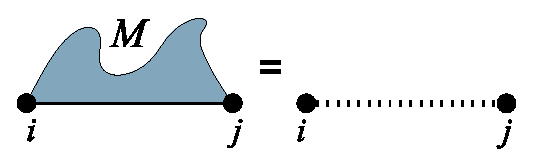
\includegraphics[width=\textwidth,height=\textheight/2,keepaspectratio=true]{decomp_ml_up}}
\end{DoxyImageNoCaption}
 \hypertarget{group__constraints_ga63d8ceb8c96ae3b463e529e28cc0fe98}{}\index{Constraining the Secondary Structure Predictions and Evaluations@{Constraining the Secondary Structure Predictions and Evaluations}!V\+R\+N\+A\+\_\+\+D\+E\+C\+O\+M\+P\+\_\+\+M\+L\+\_\+\+M\+L\+\_\+\+S\+T\+E\+M@{V\+R\+N\+A\+\_\+\+D\+E\+C\+O\+M\+P\+\_\+\+M\+L\+\_\+\+M\+L\+\_\+\+S\+T\+E\+M}}
\index{V\+R\+N\+A\+\_\+\+D\+E\+C\+O\+M\+P\+\_\+\+M\+L\+\_\+\+M\+L\+\_\+\+S\+T\+E\+M@{V\+R\+N\+A\+\_\+\+D\+E\+C\+O\+M\+P\+\_\+\+M\+L\+\_\+\+M\+L\+\_\+\+S\+T\+E\+M}!Constraining the Secondary Structure Predictions and Evaluations@{Constraining the Secondary Structure Predictions and Evaluations}}
\subsubsection[{V\+R\+N\+A\+\_\+\+D\+E\+C\+O\+M\+P\+\_\+\+M\+L\+\_\+\+M\+L\+\_\+\+S\+T\+E\+M}]{\setlength{\rightskip}{0pt plus 5cm}\#define V\+R\+N\+A\+\_\+\+D\+E\+C\+O\+M\+P\+\_\+\+M\+L\+\_\+\+M\+L\+\_\+\+S\+T\+E\+M~20}\label{group__constraints_ga63d8ceb8c96ae3b463e529e28cc0fe98}


{\ttfamily \#include $<$\hyperlink{constraints_8h}{Vienna\+R\+N\+A/constraints.\+h}$>$}



Indicator for decomposition of multibranch loop part. 

This flag notifies the soft or hard constraint callback function that the current decomposition step evaluates a multibranch loop part in the interval $[i:j]$, which will decomposed into a multibranch loop part $[i:k]$, and a stem with enclosing base pair $(l,j)$.

 
\begin{DoxyImageNoCaption}
  \mbox{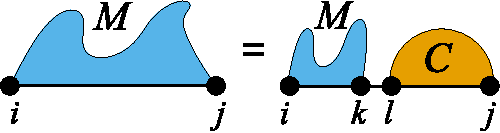
\includegraphics[width=\textwidth,height=\textheight/2,keepaspectratio=true]{decomp_ml_ml_stem}}
\end{DoxyImageNoCaption}
 \hypertarget{group__constraints_ga4fe48d575830b16c208e280e01ab1497}{}\index{Constraining the Secondary Structure Predictions and Evaluations@{Constraining the Secondary Structure Predictions and Evaluations}!V\+R\+N\+A\+\_\+\+D\+E\+C\+O\+M\+P\+\_\+\+M\+L\+\_\+\+C\+O\+A\+X\+I\+A\+L@{V\+R\+N\+A\+\_\+\+D\+E\+C\+O\+M\+P\+\_\+\+M\+L\+\_\+\+C\+O\+A\+X\+I\+A\+L}}
\index{V\+R\+N\+A\+\_\+\+D\+E\+C\+O\+M\+P\+\_\+\+M\+L\+\_\+\+C\+O\+A\+X\+I\+A\+L@{V\+R\+N\+A\+\_\+\+D\+E\+C\+O\+M\+P\+\_\+\+M\+L\+\_\+\+C\+O\+A\+X\+I\+A\+L}!Constraining the Secondary Structure Predictions and Evaluations@{Constraining the Secondary Structure Predictions and Evaluations}}
\subsubsection[{V\+R\+N\+A\+\_\+\+D\+E\+C\+O\+M\+P\+\_\+\+M\+L\+\_\+\+C\+O\+A\+X\+I\+A\+L}]{\setlength{\rightskip}{0pt plus 5cm}\#define V\+R\+N\+A\+\_\+\+D\+E\+C\+O\+M\+P\+\_\+\+M\+L\+\_\+\+C\+O\+A\+X\+I\+A\+L~13}\label{group__constraints_ga4fe48d575830b16c208e280e01ab1497}


{\ttfamily \#include $<$\hyperlink{constraints_8h}{Vienna\+R\+N\+A/constraints.\+h}$>$}



Indicator for decomposition of multibranch loop part. 

This flag notifies the soft or hard constraint callback function that the current decomposition step evaluates a multibranch loop part in the interval $[i:j]$, where two stems with enclosing pairs $(i,k)$ and $(l,j)$ are coaxially stacking onto each other.

 
\begin{DoxyImageNoCaption}
  \mbox{
\includegraphics[width=\textwidth,height=\textheight/2,keepaspectratio=true]{decomp_ml_coaxial}}
\end{DoxyImageNoCaption}
 \hypertarget{group__constraints_ga437adf5115c1999304eff26b41e4c9b6}{}\index{Constraining the Secondary Structure Predictions and Evaluations@{Constraining the Secondary Structure Predictions and Evaluations}!V\+R\+N\+A\+\_\+\+D\+E\+C\+O\+M\+P\+\_\+\+E\+X\+T\+\_\+\+E\+X\+T@{V\+R\+N\+A\+\_\+\+D\+E\+C\+O\+M\+P\+\_\+\+E\+X\+T\+\_\+\+E\+X\+T}}
\index{V\+R\+N\+A\+\_\+\+D\+E\+C\+O\+M\+P\+\_\+\+E\+X\+T\+\_\+\+E\+X\+T@{V\+R\+N\+A\+\_\+\+D\+E\+C\+O\+M\+P\+\_\+\+E\+X\+T\+\_\+\+E\+X\+T}!Constraining the Secondary Structure Predictions and Evaluations@{Constraining the Secondary Structure Predictions and Evaluations}}
\subsubsection[{V\+R\+N\+A\+\_\+\+D\+E\+C\+O\+M\+P\+\_\+\+E\+X\+T\+\_\+\+E\+X\+T}]{\setlength{\rightskip}{0pt plus 5cm}\#define V\+R\+N\+A\+\_\+\+D\+E\+C\+O\+M\+P\+\_\+\+E\+X\+T\+\_\+\+E\+X\+T~9}\label{group__constraints_ga437adf5115c1999304eff26b41e4c9b6}


{\ttfamily \#include $<$\hyperlink{constraints_8h}{Vienna\+R\+N\+A/constraints.\+h}$>$}



Indicator for decomposition of exterior loop part. 

This flag notifies the soft or hard constraint callback function that the current decomposition step evaluates an exterior loop part in the interval $[i:j]$, which will be decomposed into a (usually) smaller exterior loop part $[k:l]$.

 
\begin{DoxyImageNoCaption}
  \mbox{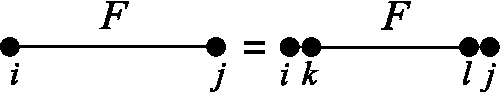
\includegraphics[width=\textwidth,height=\textheight/2,keepaspectratio=true]{decomp_ext_ext}}
\end{DoxyImageNoCaption}
 \hypertarget{group__constraints_gaff1ddaffe86d984623910b40cc8a8717}{}\index{Constraining the Secondary Structure Predictions and Evaluations@{Constraining the Secondary Structure Predictions and Evaluations}!V\+R\+N\+A\+\_\+\+D\+E\+C\+O\+M\+P\+\_\+\+E\+X\+T\+\_\+\+U\+P@{V\+R\+N\+A\+\_\+\+D\+E\+C\+O\+M\+P\+\_\+\+E\+X\+T\+\_\+\+U\+P}}
\index{V\+R\+N\+A\+\_\+\+D\+E\+C\+O\+M\+P\+\_\+\+E\+X\+T\+\_\+\+U\+P@{V\+R\+N\+A\+\_\+\+D\+E\+C\+O\+M\+P\+\_\+\+E\+X\+T\+\_\+\+U\+P}!Constraining the Secondary Structure Predictions and Evaluations@{Constraining the Secondary Structure Predictions and Evaluations}}
\subsubsection[{V\+R\+N\+A\+\_\+\+D\+E\+C\+O\+M\+P\+\_\+\+E\+X\+T\+\_\+\+U\+P}]{\setlength{\rightskip}{0pt plus 5cm}\#define V\+R\+N\+A\+\_\+\+D\+E\+C\+O\+M\+P\+\_\+\+E\+X\+T\+\_\+\+U\+P~8}\label{group__constraints_gaff1ddaffe86d984623910b40cc8a8717}


{\ttfamily \#include $<$\hyperlink{constraints_8h}{Vienna\+R\+N\+A/constraints.\+h}$>$}



Indicator for decomposition of exterior loop part. 

This flag notifies the soft or hard constraint callback function that the current decomposition step evaluates an exterior loop part in the interval $[i:j]$, which will be considered as an exterior loop component consisting of only unpaired nucleotides.

 
\begin{DoxyImageNoCaption}
  \mbox{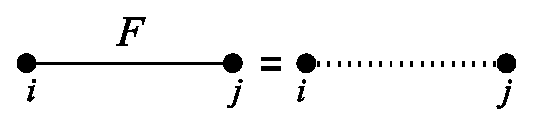
\includegraphics[width=\textwidth,height=\textheight/2,keepaspectratio=true]{decomp_ext_up}}
\end{DoxyImageNoCaption}
 \hypertarget{group__constraints_gae44b5ace0d9b4a29088069ecb4cec441}{}\index{Constraining the Secondary Structure Predictions and Evaluations@{Constraining the Secondary Structure Predictions and Evaluations}!V\+R\+N\+A\+\_\+\+D\+E\+C\+O\+M\+P\+\_\+\+E\+X\+T\+\_\+\+S\+T\+E\+M@{V\+R\+N\+A\+\_\+\+D\+E\+C\+O\+M\+P\+\_\+\+E\+X\+T\+\_\+\+S\+T\+E\+M}}
\index{V\+R\+N\+A\+\_\+\+D\+E\+C\+O\+M\+P\+\_\+\+E\+X\+T\+\_\+\+S\+T\+E\+M@{V\+R\+N\+A\+\_\+\+D\+E\+C\+O\+M\+P\+\_\+\+E\+X\+T\+\_\+\+S\+T\+E\+M}!Constraining the Secondary Structure Predictions and Evaluations@{Constraining the Secondary Structure Predictions and Evaluations}}
\subsubsection[{V\+R\+N\+A\+\_\+\+D\+E\+C\+O\+M\+P\+\_\+\+E\+X\+T\+\_\+\+S\+T\+E\+M}]{\setlength{\rightskip}{0pt plus 5cm}\#define V\+R\+N\+A\+\_\+\+D\+E\+C\+O\+M\+P\+\_\+\+E\+X\+T\+\_\+\+S\+T\+E\+M~14}\label{group__constraints_gae44b5ace0d9b4a29088069ecb4cec441}


{\ttfamily \#include $<$\hyperlink{constraints_8h}{Vienna\+R\+N\+A/constraints.\+h}$>$}



Indicator for decomposition of exterior loop part. 

This flag notifies the soft or hard constraint callback function that the current decomposition step evaluates an exterior loop part in the interval $[i:j]$, which will be considered a stem with enclosing pair $(k,l)$.

 
\begin{DoxyImageNoCaption}
  \mbox{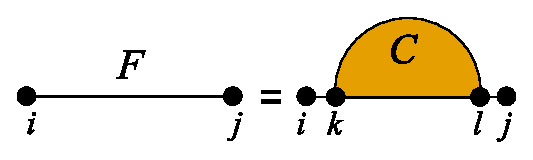
\includegraphics[width=\textwidth,height=\textheight/2,keepaspectratio=true]{decomp_ext_stem}}
\end{DoxyImageNoCaption}
 \hypertarget{group__constraints_ga803bd818b3f4b2b0a4a5cfa2f7dc2045}{}\index{Constraining the Secondary Structure Predictions and Evaluations@{Constraining the Secondary Structure Predictions and Evaluations}!V\+R\+N\+A\+\_\+\+D\+E\+C\+O\+M\+P\+\_\+\+E\+X\+T\+\_\+\+E\+X\+T\+\_\+\+E\+X\+T@{V\+R\+N\+A\+\_\+\+D\+E\+C\+O\+M\+P\+\_\+\+E\+X\+T\+\_\+\+E\+X\+T\+\_\+\+E\+X\+T}}
\index{V\+R\+N\+A\+\_\+\+D\+E\+C\+O\+M\+P\+\_\+\+E\+X\+T\+\_\+\+E\+X\+T\+\_\+\+E\+X\+T@{V\+R\+N\+A\+\_\+\+D\+E\+C\+O\+M\+P\+\_\+\+E\+X\+T\+\_\+\+E\+X\+T\+\_\+\+E\+X\+T}!Constraining the Secondary Structure Predictions and Evaluations@{Constraining the Secondary Structure Predictions and Evaluations}}
\subsubsection[{V\+R\+N\+A\+\_\+\+D\+E\+C\+O\+M\+P\+\_\+\+E\+X\+T\+\_\+\+E\+X\+T\+\_\+\+E\+X\+T}]{\setlength{\rightskip}{0pt plus 5cm}\#define V\+R\+N\+A\+\_\+\+D\+E\+C\+O\+M\+P\+\_\+\+E\+X\+T\+\_\+\+E\+X\+T\+\_\+\+E\+X\+T~15}\label{group__constraints_ga803bd818b3f4b2b0a4a5cfa2f7dc2045}


{\ttfamily \#include $<$\hyperlink{constraints_8h}{Vienna\+R\+N\+A/constraints.\+h}$>$}



Indicator for decomposition of exterior loop part. 

This flag notifies the soft or hard constraint callback function that the current decomposition step evaluates an exterior loop part in the interval $[i:j]$, which will be decomposed into two exterior loop parts $[i:k]$ and $[l:j]$.

 
\begin{DoxyImageNoCaption}
  \mbox{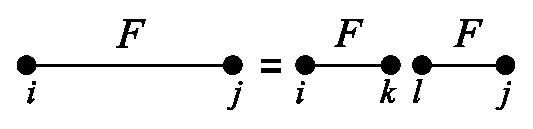
\includegraphics[width=\textwidth,height=\textheight/2,keepaspectratio=true]{decomp_ext_ext_ext}}
\end{DoxyImageNoCaption}
 \hypertarget{group__constraints_gabb09c5b78b75a44502fc77b950125c1e}{}\index{Constraining the Secondary Structure Predictions and Evaluations@{Constraining the Secondary Structure Predictions and Evaluations}!V\+R\+N\+A\+\_\+\+D\+E\+C\+O\+M\+P\+\_\+\+E\+X\+T\+\_\+\+S\+T\+E\+M\+\_\+\+E\+X\+T@{V\+R\+N\+A\+\_\+\+D\+E\+C\+O\+M\+P\+\_\+\+E\+X\+T\+\_\+\+S\+T\+E\+M\+\_\+\+E\+X\+T}}
\index{V\+R\+N\+A\+\_\+\+D\+E\+C\+O\+M\+P\+\_\+\+E\+X\+T\+\_\+\+S\+T\+E\+M\+\_\+\+E\+X\+T@{V\+R\+N\+A\+\_\+\+D\+E\+C\+O\+M\+P\+\_\+\+E\+X\+T\+\_\+\+S\+T\+E\+M\+\_\+\+E\+X\+T}!Constraining the Secondary Structure Predictions and Evaluations@{Constraining the Secondary Structure Predictions and Evaluations}}
\subsubsection[{V\+R\+N\+A\+\_\+\+D\+E\+C\+O\+M\+P\+\_\+\+E\+X\+T\+\_\+\+S\+T\+E\+M\+\_\+\+E\+X\+T}]{\setlength{\rightskip}{0pt plus 5cm}\#define V\+R\+N\+A\+\_\+\+D\+E\+C\+O\+M\+P\+\_\+\+E\+X\+T\+\_\+\+S\+T\+E\+M\+\_\+\+E\+X\+T~16}\label{group__constraints_gabb09c5b78b75a44502fc77b950125c1e}


{\ttfamily \#include $<$\hyperlink{constraints_8h}{Vienna\+R\+N\+A/constraints.\+h}$>$}



Indicator for decomposition of exterior loop part. 

This flag notifies the soft or hard constraint callback function that the current decomposition step evaluates an exterior loop part in the interval $[i:j]$, which will be decomposed into a stem branching off with base pair $(i,k)$, and an exterior loop part $[l:j]$.

 
\begin{DoxyImageNoCaption}
  \mbox{
\includegraphics[width=\textwidth,height=\textheight/2,keepaspectratio=true]{decomp_ext_stem_ext}}
\end{DoxyImageNoCaption}
 \hypertarget{group__constraints_ga06efd054c9271438f6d82d4559d9e69f}{}\index{Constraining the Secondary Structure Predictions and Evaluations@{Constraining the Secondary Structure Predictions and Evaluations}!V\+R\+N\+A\+\_\+\+D\+E\+C\+O\+M\+P\+\_\+\+E\+X\+T\+\_\+\+E\+X\+T\+\_\+\+S\+T\+E\+M@{V\+R\+N\+A\+\_\+\+D\+E\+C\+O\+M\+P\+\_\+\+E\+X\+T\+\_\+\+E\+X\+T\+\_\+\+S\+T\+E\+M}}
\index{V\+R\+N\+A\+\_\+\+D\+E\+C\+O\+M\+P\+\_\+\+E\+X\+T\+\_\+\+E\+X\+T\+\_\+\+S\+T\+E\+M@{V\+R\+N\+A\+\_\+\+D\+E\+C\+O\+M\+P\+\_\+\+E\+X\+T\+\_\+\+E\+X\+T\+\_\+\+S\+T\+E\+M}!Constraining the Secondary Structure Predictions and Evaluations@{Constraining the Secondary Structure Predictions and Evaluations}}
\subsubsection[{V\+R\+N\+A\+\_\+\+D\+E\+C\+O\+M\+P\+\_\+\+E\+X\+T\+\_\+\+E\+X\+T\+\_\+\+S\+T\+E\+M}]{\setlength{\rightskip}{0pt plus 5cm}\#define V\+R\+N\+A\+\_\+\+D\+E\+C\+O\+M\+P\+\_\+\+E\+X\+T\+\_\+\+E\+X\+T\+\_\+\+S\+T\+E\+M~18}\label{group__constraints_ga06efd054c9271438f6d82d4559d9e69f}


{\ttfamily \#include $<$\hyperlink{constraints_8h}{Vienna\+R\+N\+A/constraints.\+h}$>$}



Indicator for decomposition of exterior loop part. 

This flag notifies the soft or hard constraint callback function that the current decomposition step evaluates an exterior loop part in the interval $[i:j]$, which will be decomposed into an exterior loop part $[i:k]$, and a stem branching off with base pair $(l,j)$.

 
\begin{DoxyImageNoCaption}
  \mbox{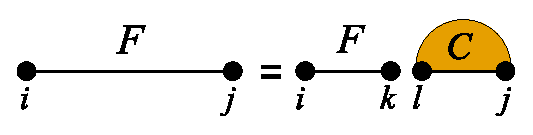
\includegraphics[width=\textwidth,height=\textheight/2,keepaspectratio=true]{decomp_ext_ext_stem}}
\end{DoxyImageNoCaption}
 \hypertarget{group__constraints_ga2e75d7a77118735b32f25422d9686719}{}\index{Constraining the Secondary Structure Predictions and Evaluations@{Constraining the Secondary Structure Predictions and Evaluations}!V\+R\+N\+A\+\_\+\+D\+E\+C\+O\+M\+P\+\_\+\+E\+X\+T\+\_\+\+E\+X\+T\+\_\+\+S\+T\+E\+M1@{V\+R\+N\+A\+\_\+\+D\+E\+C\+O\+M\+P\+\_\+\+E\+X\+T\+\_\+\+E\+X\+T\+\_\+\+S\+T\+E\+M1}}
\index{V\+R\+N\+A\+\_\+\+D\+E\+C\+O\+M\+P\+\_\+\+E\+X\+T\+\_\+\+E\+X\+T\+\_\+\+S\+T\+E\+M1@{V\+R\+N\+A\+\_\+\+D\+E\+C\+O\+M\+P\+\_\+\+E\+X\+T\+\_\+\+E\+X\+T\+\_\+\+S\+T\+E\+M1}!Constraining the Secondary Structure Predictions and Evaluations@{Constraining the Secondary Structure Predictions and Evaluations}}
\subsubsection[{V\+R\+N\+A\+\_\+\+D\+E\+C\+O\+M\+P\+\_\+\+E\+X\+T\+\_\+\+E\+X\+T\+\_\+\+S\+T\+E\+M1}]{\setlength{\rightskip}{0pt plus 5cm}\#define V\+R\+N\+A\+\_\+\+D\+E\+C\+O\+M\+P\+\_\+\+E\+X\+T\+\_\+\+E\+X\+T\+\_\+\+S\+T\+E\+M1~19}\label{group__constraints_ga2e75d7a77118735b32f25422d9686719}


{\ttfamily \#include $<$\hyperlink{constraints_8h}{Vienna\+R\+N\+A/constraints.\+h}$>$}



Indicator for decomposition of exterior loop part. 

This flag notifies the soft or hard constraint callback function that the current decomposition step evaluates an exterior loop part in the interval $[i:j]$, which will be decomposed into an exterior loop part $[i:k]$, and a stem branching off with base pair $(l,j-1)$.

 
\begin{DoxyImageNoCaption}
  \mbox{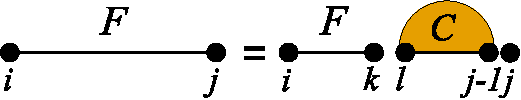
\includegraphics[width=\textwidth,height=\textheight/2,keepaspectratio=true]{decomp_ext_ext_stem1}}
\end{DoxyImageNoCaption}
 

\subsection{Function Documentation}
\hypertarget{group__constraints_ga35a401f680969a556858a8dd5f1d07cc}{}\index{Constraining the Secondary Structure Predictions and Evaluations@{Constraining the Secondary Structure Predictions and Evaluations}!vrna\+\_\+constraints\+\_\+add@{vrna\+\_\+constraints\+\_\+add}}
\index{vrna\+\_\+constraints\+\_\+add@{vrna\+\_\+constraints\+\_\+add}!Constraining the Secondary Structure Predictions and Evaluations@{Constraining the Secondary Structure Predictions and Evaluations}}
\subsubsection[{vrna\+\_\+constraints\+\_\+add}]{\setlength{\rightskip}{0pt plus 5cm}void vrna\+\_\+constraints\+\_\+add (
\begin{DoxyParamCaption}
\item[{{\bf vrna\+\_\+fold\+\_\+compound\+\_\+t} $\ast$}]{vc, }
\item[{const char $\ast$}]{constraint, }
\item[{unsigned int}]{options}
\end{DoxyParamCaption}
)}\label{group__constraints_ga35a401f680969a556858a8dd5f1d07cc}


{\ttfamily \#include $<$\hyperlink{constraints_8h}{Vienna\+R\+N\+A/constraints.\+h}$>$}



Add constraints to a \hyperlink{group__fold__compound_ga1b0cef17fd40466cef5968eaeeff6166}{vrna\+\_\+fold\+\_\+compound\+\_\+t} data structure. 

Use this function to add/update the hard/soft constraints The function allows for passing a string \textquotesingle{}constraint\textquotesingle{} that can either be a filename that points to a constraints definition file or it may be a pseudo dot-\/bracket notation indicating hard constraints. For the latter, the user has to pass the \hyperlink{group__hard__constraints_ga4bfc2f15c4f261c62a11af9d2aa80c90}{V\+R\+N\+A\+\_\+\+C\+O\+N\+S\+T\+R\+A\+I\+N\+T\+\_\+\+D\+B} option. Also, the user has to specify, which characters are allowed to be interpreted as constraints by passing the corresponding options via the third parameter.

\begin{DoxySeeAlso}{See also}
\hyperlink{group__hard__constraints_ga36ff456c43bf920629cee5a236e4f0ff}{vrna\+\_\+hc\+\_\+init()}, \hyperlink{group__hard__constraints_gaeb352e3e6ccd2b567bafa451365bb545}{vrna\+\_\+hc\+\_\+add\+\_\+up()}, \hyperlink{group__hard__constraints_ga5070f296c8af2baea10951525519464f}{vrna\+\_\+hc\+\_\+add\+\_\+up\+\_\+batch()}, \hyperlink{group__hard__constraints_gac49305fc5c7d8653c5fbd2de1e1615e2}{vrna\+\_\+hc\+\_\+add\+\_\+bp()}, \hyperlink{group__soft__constraints_ga9d977a1681356778cc66dceafbe5b032}{vrna\+\_\+sc\+\_\+init()}, \hyperlink{group__soft__constraints_ga30f30c8eff9676775a3e831d972b5284}{vrna\+\_\+sc\+\_\+add\+\_\+up()}, \hyperlink{group__soft__constraints_ga86049d4bb0ea8674cae9b6177156b184}{vrna\+\_\+sc\+\_\+add\+\_\+bp()}, \hyperlink{group__SHAPE__reactivities_ga57d612b58e1c61dd6cfcb5a843f8f1b3}{vrna\+\_\+sc\+\_\+add\+\_\+\+S\+H\+A\+P\+E\+\_\+deigan()}, \hyperlink{group__SHAPE__reactivities_gaf3c65a045060aef5c4e41693d30af58c}{vrna\+\_\+sc\+\_\+add\+\_\+\+S\+H\+A\+P\+E\+\_\+zarringhalam()}, \hyperlink{group__hard__constraints_ga696dcf77887d856c6f21ea266d8b9ca2}{vrna\+\_\+hc\+\_\+free()}, \hyperlink{group__soft__constraints_ga6d55446448d69346fc313b993c4fb3e8}{vrna\+\_\+sc\+\_\+free()}, \hyperlink{group__hard__constraints_ga4bfc2f15c4f261c62a11af9d2aa80c90}{V\+R\+N\+A\+\_\+\+C\+O\+N\+S\+T\+R\+A\+I\+N\+T\+\_\+\+D\+B}, \hyperlink{group__hard__constraints_ga1c3864bdc92147a4d93de2b1b4356177}{V\+R\+N\+A\+\_\+\+C\+O\+N\+S\+T\+R\+A\+I\+N\+T\+\_\+\+D\+B\+\_\+\+D\+E\+F\+A\+U\+L\+T}, \hyperlink{group__hard__constraints_ga13053547a2de5532b64b64d35e097ae1}{V\+R\+N\+A\+\_\+\+C\+O\+N\+S\+T\+R\+A\+I\+N\+T\+\_\+\+D\+B\+\_\+\+P\+I\+P\+E}, \hyperlink{group__hard__constraints_ga369bea82eae75fbe626f409fa425747e}{V\+R\+N\+A\+\_\+\+C\+O\+N\+S\+T\+R\+A\+I\+N\+T\+\_\+\+D\+B\+\_\+\+D\+O\+T}, \hyperlink{group__hard__constraints_ga7283bbe0f8954f7b030ecc3f2d1932b2}{V\+R\+N\+A\+\_\+\+C\+O\+N\+S\+T\+R\+A\+I\+N\+T\+\_\+\+D\+B\+\_\+\+X}, \hyperlink{constraints__hard_8h_ad54c1315a47d55653dcaa5de6e544b77}{V\+R\+N\+A\+\_\+\+C\+O\+N\+S\+T\+R\+A\+I\+N\+T\+\_\+\+D\+B\+\_\+\+A\+N\+G\+\_\+\+B\+R\+A\+C\+K}, \hyperlink{group__hard__constraints_gac17b034852c914bc5879954c65d7e74b}{V\+R\+N\+A\+\_\+\+C\+O\+N\+S\+T\+R\+A\+I\+N\+T\+\_\+\+D\+B\+\_\+\+R\+N\+D\+\_\+\+B\+R\+A\+C\+K}, \hyperlink{group__hard__constraints_ga5c17253f5a39d1d49b0fb11f5196982a}{V\+R\+N\+A\+\_\+\+C\+O\+N\+S\+T\+R\+A\+I\+N\+T\+\_\+\+D\+B\+\_\+\+I\+N\+T\+R\+A\+M\+O\+L}, \hyperlink{group__hard__constraints_ga31d0ebb9755ca8a4acafc14f00ca755d}{V\+R\+N\+A\+\_\+\+C\+O\+N\+S\+T\+R\+A\+I\+N\+T\+\_\+\+D\+B\+\_\+\+I\+N\+T\+E\+R\+M\+O\+L}, \hyperlink{group__hard__constraints_ga75cfab03cdc97c95b3ce8bb29f52b08e}{V\+R\+N\+A\+\_\+\+C\+O\+N\+S\+T\+R\+A\+I\+N\+T\+\_\+\+D\+B\+\_\+\+G\+Q\+U\+A\+D}
\end{DoxySeeAlso}
The following is an example for adding hard constraints given in pseudo dot-\/bracket notation. Here, {\ttfamily vc} is the \hyperlink{group__fold__compound_ga1b0cef17fd40466cef5968eaeeff6166}{vrna\+\_\+fold\+\_\+compound\+\_\+t} object, {\ttfamily structure} is a char array with the hard constraint in dot-\/bracket notation, and {\ttfamily enforce\+Constraints} is a flag indicating whether or not constraints for base pairs should be enforced instead of just doing a removal of base pair that conflict with the constraint.


\begin{DoxyCodeInclude}
          \textcolor{keywordtype}{unsigned} \textcolor{keywordtype}{int} constraint\_options = \hyperlink{group__hard__constraints_ga1c3864bdc92147a4d93de2b1b4356177}{VRNA\_CONSTRAINT\_DB\_DEFAULT};
          \textcolor{keywordflow}{if}(enforceConstraints)
            constraint\_options |= \hyperlink{group__hard__constraints_ga29ebe940110d60ab798fdacbcdbbfb7d}{VRNA\_CONSTRAINT\_DB\_ENFORCE\_BP};
          \hyperlink{group__constraints_ga35a401f680969a556858a8dd5f1d07cc}{vrna\_constraints\_add}(vc, (\textcolor{keyword}{const} \textcolor{keywordtype}{char} *)structure, constraint\_options);
\end{DoxyCodeInclude}
 In constrat to the above, constraints may also be read from file\+:


\begin{DoxyCodeInclude}
        \hyperlink{group__constraints_ga35a401f680969a556858a8dd5f1d07cc}{vrna\_constraints\_add}(vc, constraints\_file, 
      \hyperlink{group__fold__compound_gae63be9127fe7dcc1f9bb14f5bb1064ee}{VRNA\_OPTION\_MFE} | ((pf) ? \hyperlink{group__fold__compound_gabfbadcddda3e74ce7f49035ef8f058f7}{VRNA\_OPTION\_PF} : 0));
\end{DoxyCodeInclude}
 \begin{DoxySeeAlso}{See also}
\hyperlink{group__hard__constraints_ga5b4de3247b67358080c176b94591a8e6}{vrna\+\_\+hc\+\_\+add\+\_\+from\+\_\+db()}, \hyperlink{group__hard__constraints_gaeb352e3e6ccd2b567bafa451365bb545}{vrna\+\_\+hc\+\_\+add\+\_\+up()}, \hyperlink{group__hard__constraints_ga5070f296c8af2baea10951525519464f}{vrna\+\_\+hc\+\_\+add\+\_\+up\+\_\+batch()} vrna\+\_\+hc\+\_\+add\+\_\+bp\+\_\+unspecific(), \hyperlink{group__hard__constraints_gac49305fc5c7d8653c5fbd2de1e1615e2}{vrna\+\_\+hc\+\_\+add\+\_\+bp()}
\end{DoxySeeAlso}

\begin{DoxyParams}{Parameters}
{\em vc} & The fold compound \\
\hline
{\em constraint} & A string with either the filename of the constraint definitions or a pseudo dot-\/bracket notation of the hard constraint. May be N\+U\+L\+L. \\
\hline
{\em options} & The option flags \\
\hline
\end{DoxyParams}
\hypertarget{group__constraints_gaa1f20b53bf09ac2e6b0dbb13f7d89670}{}\index{Constraining the Secondary Structure Predictions and Evaluations@{Constraining the Secondary Structure Predictions and Evaluations}!vrna\+\_\+message\+\_\+constraint\+\_\+options@{vrna\+\_\+message\+\_\+constraint\+\_\+options}}
\index{vrna\+\_\+message\+\_\+constraint\+\_\+options@{vrna\+\_\+message\+\_\+constraint\+\_\+options}!Constraining the Secondary Structure Predictions and Evaluations@{Constraining the Secondary Structure Predictions and Evaluations}}
\subsubsection[{vrna\+\_\+message\+\_\+constraint\+\_\+options}]{\setlength{\rightskip}{0pt plus 5cm}void vrna\+\_\+message\+\_\+constraint\+\_\+options (
\begin{DoxyParamCaption}
\item[{unsigned int}]{option}
\end{DoxyParamCaption}
)}\label{group__constraints_gaa1f20b53bf09ac2e6b0dbb13f7d89670}


{\ttfamily \#include $<$\hyperlink{constraints__hard_8h}{Vienna\+R\+N\+A/constraints\+\_\+hard.\+h}$>$}



Print a help message for pseudo dot-\/bracket structure constraint characters to stdout. (constraint support is specified by option parameter) 

Currently available options are\+:~\newline
\hyperlink{group__hard__constraints_ga13053547a2de5532b64b64d35e097ae1}{V\+R\+N\+A\+\_\+\+C\+O\+N\+S\+T\+R\+A\+I\+N\+T\+\_\+\+D\+B\+\_\+\+P\+I\+P\+E} (paired with another base)~\newline
\hyperlink{group__hard__constraints_ga369bea82eae75fbe626f409fa425747e}{V\+R\+N\+A\+\_\+\+C\+O\+N\+S\+T\+R\+A\+I\+N\+T\+\_\+\+D\+B\+\_\+\+D\+O\+T} (no constraint at all)~\newline
\hyperlink{group__hard__constraints_ga7283bbe0f8954f7b030ecc3f2d1932b2}{V\+R\+N\+A\+\_\+\+C\+O\+N\+S\+T\+R\+A\+I\+N\+T\+\_\+\+D\+B\+\_\+\+X} (base must not pair)~\newline
\hyperlink{constraints__hard_8h_ad54c1315a47d55653dcaa5de6e544b77}{V\+R\+N\+A\+\_\+\+C\+O\+N\+S\+T\+R\+A\+I\+N\+T\+\_\+\+D\+B\+\_\+\+A\+N\+G\+\_\+\+B\+R\+A\+C\+K} (paired downstream/upstream)~\newline
\hyperlink{group__hard__constraints_gac17b034852c914bc5879954c65d7e74b}{V\+R\+N\+A\+\_\+\+C\+O\+N\+S\+T\+R\+A\+I\+N\+T\+\_\+\+D\+B\+\_\+\+R\+N\+D\+\_\+\+B\+R\+A\+C\+K} (base i pairs base j)~\newline
 pass a collection of options as one value like this\+: \begin{DoxyVerb}vrna_message_constraints(option_1 | option_2 | option_n) \end{DoxyVerb}


\begin{DoxySeeAlso}{See also}
\hyperlink{group__constraints_gaec7e13fa0465c2acc7a621d1aecb709f}{vrna\+\_\+message\+\_\+constraint\+\_\+options\+\_\+all()}, \hyperlink{group__constraints_ga35a401f680969a556858a8dd5f1d07cc}{vrna\+\_\+constraints\+\_\+add()}, \hyperlink{group__hard__constraints_ga4bfc2f15c4f261c62a11af9d2aa80c90}{V\+R\+N\+A\+\_\+\+C\+O\+N\+S\+T\+R\+A\+I\+N\+T\+\_\+\+D\+B}, \hyperlink{group__hard__constraints_ga13053547a2de5532b64b64d35e097ae1}{V\+R\+N\+A\+\_\+\+C\+O\+N\+S\+T\+R\+A\+I\+N\+T\+\_\+\+D\+B\+\_\+\+P\+I\+P\+E}, \hyperlink{group__hard__constraints_ga369bea82eae75fbe626f409fa425747e}{V\+R\+N\+A\+\_\+\+C\+O\+N\+S\+T\+R\+A\+I\+N\+T\+\_\+\+D\+B\+\_\+\+D\+O\+T}, \hyperlink{group__hard__constraints_ga7283bbe0f8954f7b030ecc3f2d1932b2}{V\+R\+N\+A\+\_\+\+C\+O\+N\+S\+T\+R\+A\+I\+N\+T\+\_\+\+D\+B\+\_\+\+X}, \hyperlink{constraints__hard_8h_ad54c1315a47d55653dcaa5de6e544b77}{V\+R\+N\+A\+\_\+\+C\+O\+N\+S\+T\+R\+A\+I\+N\+T\+\_\+\+D\+B\+\_\+\+A\+N\+G\+\_\+\+B\+R\+A\+C\+K}, \hyperlink{group__hard__constraints_gac17b034852c914bc5879954c65d7e74b}{V\+R\+N\+A\+\_\+\+C\+O\+N\+S\+T\+R\+A\+I\+N\+T\+\_\+\+D\+B\+\_\+\+R\+N\+D\+\_\+\+B\+R\+A\+C\+K}, \hyperlink{group__hard__constraints_ga31d0ebb9755ca8a4acafc14f00ca755d}{V\+R\+N\+A\+\_\+\+C\+O\+N\+S\+T\+R\+A\+I\+N\+T\+\_\+\+D\+B\+\_\+\+I\+N\+T\+E\+R\+M\+O\+L}, \hyperlink{group__hard__constraints_ga5c17253f5a39d1d49b0fb11f5196982a}{V\+R\+N\+A\+\_\+\+C\+O\+N\+S\+T\+R\+A\+I\+N\+T\+\_\+\+D\+B\+\_\+\+I\+N\+T\+R\+A\+M\+O\+L}
\end{DoxySeeAlso}

\begin{DoxyParams}{Parameters}
{\em option} & Option switch that tells which constraint help will be printed \\
\hline
\end{DoxyParams}
\hypertarget{group__constraints_gaec7e13fa0465c2acc7a621d1aecb709f}{}\index{Constraining the Secondary Structure Predictions and Evaluations@{Constraining the Secondary Structure Predictions and Evaluations}!vrna\+\_\+message\+\_\+constraint\+\_\+options\+\_\+all@{vrna\+\_\+message\+\_\+constraint\+\_\+options\+\_\+all}}
\index{vrna\+\_\+message\+\_\+constraint\+\_\+options\+\_\+all@{vrna\+\_\+message\+\_\+constraint\+\_\+options\+\_\+all}!Constraining the Secondary Structure Predictions and Evaluations@{Constraining the Secondary Structure Predictions and Evaluations}}
\subsubsection[{vrna\+\_\+message\+\_\+constraint\+\_\+options\+\_\+all}]{\setlength{\rightskip}{0pt plus 5cm}void vrna\+\_\+message\+\_\+constraint\+\_\+options\+\_\+all (
\begin{DoxyParamCaption}
\item[{void}]{}
\end{DoxyParamCaption}
)}\label{group__constraints_gaec7e13fa0465c2acc7a621d1aecb709f}


{\ttfamily \#include $<$\hyperlink{constraints__hard_8h}{Vienna\+R\+N\+A/constraints\+\_\+hard.\+h}$>$}



Print structure constraint characters to stdout (full constraint support) 

\begin{DoxySeeAlso}{See also}
\hyperlink{group__constraints_gaa1f20b53bf09ac2e6b0dbb13f7d89670}{vrna\+\_\+message\+\_\+constraint\+\_\+options()}, \hyperlink{group__constraints_ga35a401f680969a556858a8dd5f1d07cc}{vrna\+\_\+constraints\+\_\+add()}, \hyperlink{group__hard__constraints_ga4bfc2f15c4f261c62a11af9d2aa80c90}{V\+R\+N\+A\+\_\+\+C\+O\+N\+S\+T\+R\+A\+I\+N\+T\+\_\+\+D\+B}, \hyperlink{group__hard__constraints_ga13053547a2de5532b64b64d35e097ae1}{V\+R\+N\+A\+\_\+\+C\+O\+N\+S\+T\+R\+A\+I\+N\+T\+\_\+\+D\+B\+\_\+\+P\+I\+P\+E}, \hyperlink{group__hard__constraints_ga369bea82eae75fbe626f409fa425747e}{V\+R\+N\+A\+\_\+\+C\+O\+N\+S\+T\+R\+A\+I\+N\+T\+\_\+\+D\+B\+\_\+\+D\+O\+T}, \hyperlink{group__hard__constraints_ga7283bbe0f8954f7b030ecc3f2d1932b2}{V\+R\+N\+A\+\_\+\+C\+O\+N\+S\+T\+R\+A\+I\+N\+T\+\_\+\+D\+B\+\_\+\+X}, \hyperlink{constraints__hard_8h_ad54c1315a47d55653dcaa5de6e544b77}{V\+R\+N\+A\+\_\+\+C\+O\+N\+S\+T\+R\+A\+I\+N\+T\+\_\+\+D\+B\+\_\+\+A\+N\+G\+\_\+\+B\+R\+A\+C\+K}, \hyperlink{group__hard__constraints_gac17b034852c914bc5879954c65d7e74b}{V\+R\+N\+A\+\_\+\+C\+O\+N\+S\+T\+R\+A\+I\+N\+T\+\_\+\+D\+B\+\_\+\+R\+N\+D\+\_\+\+B\+R\+A\+C\+K}, \hyperlink{group__hard__constraints_ga31d0ebb9755ca8a4acafc14f00ca755d}{V\+R\+N\+A\+\_\+\+C\+O\+N\+S\+T\+R\+A\+I\+N\+T\+\_\+\+D\+B\+\_\+\+I\+N\+T\+E\+R\+M\+O\+L}, \hyperlink{group__hard__constraints_ga5c17253f5a39d1d49b0fb11f5196982a}{V\+R\+N\+A\+\_\+\+C\+O\+N\+S\+T\+R\+A\+I\+N\+T\+\_\+\+D\+B\+\_\+\+I\+N\+T\+R\+A\+M\+O\+L} 
\end{DoxySeeAlso}

\hypertarget{group__data__structures}{}\section{Data Structures and Preprocessor Macros}
\label{group__data__structures}\index{Data Structures and Preprocessor Macros@{Data Structures and Preprocessor Macros}}


All datastructures and typedefs shared among the Vienna R\+N\+A Package can be found here.  


Collaboration diagram for Data Structures and Preprocessor Macros\+:
\nopagebreak
\begin{figure}[H]
\begin{center}
\leavevmode
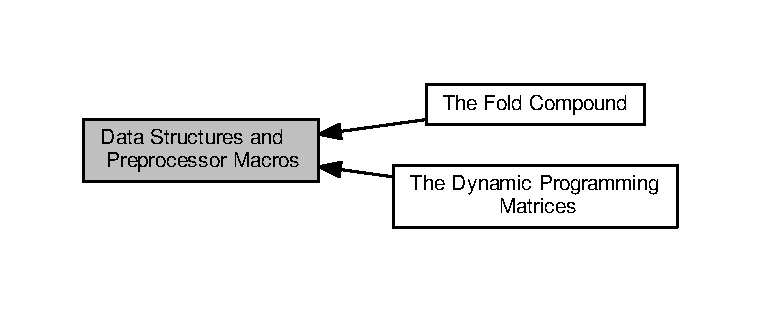
\includegraphics[width=350pt]{group__data__structures}
\end{center}
\end{figure}
\subsection*{Modules}
\begin{DoxyCompactItemize}
\item 
\hyperlink{group__fold__compound}{The Fold Compound}
\begin{DoxyCompactList}\small\item\em This module provides interfaces that deal with the most basic data structure used in structure predicting and energy evaluating function of the R\+N\+Alib. \end{DoxyCompactList}\item 
\hyperlink{group__dp__matrices}{The Dynamic Programming Matrices}
\begin{DoxyCompactList}\small\item\em This module provides interfaces that deal with creation and destruction of dynamic programming matrices used within the R\+N\+Alib. \end{DoxyCompactList}\end{DoxyCompactItemize}
\subsection*{Data Structures}
\begin{DoxyCompactItemize}
\item 
struct \hyperlink{group__data__structures_structvrna__basepair__s}{vrna\+\_\+basepair\+\_\+s}
\begin{DoxyCompactList}\small\item\em Base pair data structure used in subopt.\+c.  \hyperlink{group__data__structures_structvrna__basepair__s}{More...}\end{DoxyCompactList}\item 
struct \hyperlink{group__data__structures_structvrna__plist__s}{vrna\+\_\+plist\+\_\+s}
\begin{DoxyCompactList}\small\item\em this datastructure is used as input parameter in functions of \hyperlink{PS__dot_8h}{P\+S\+\_\+dot.\+h} and others  \hyperlink{group__data__structures_structvrna__plist__s}{More...}\end{DoxyCompactList}\item 
struct \hyperlink{group__data__structures_structvrna__cpair__s}{vrna\+\_\+cpair\+\_\+s}
\begin{DoxyCompactList}\small\item\em this datastructure is used as input parameter in functions of P\+S\+\_\+dot.\+c  \hyperlink{group__data__structures_structvrna__cpair__s}{More...}\end{DoxyCompactList}\item 
struct \hyperlink{group__data__structures_structvrna__sect__s}{vrna\+\_\+sect\+\_\+s}
\begin{DoxyCompactList}\small\item\em Stack of partial structures for backtracking.  \hyperlink{group__data__structures_structvrna__sect__s}{More...}\end{DoxyCompactList}\item 
struct \hyperlink{group__data__structures_structvrna__bp__stack__s}{vrna\+\_\+bp\+\_\+stack\+\_\+s}
\begin{DoxyCompactList}\small\item\em Base pair stack element.  \hyperlink{group__data__structures_structvrna__bp__stack__s}{More...}\end{DoxyCompactList}\item 
struct \hyperlink{group__data__structures_structpu__contrib}{pu\+\_\+contrib}
\begin{DoxyCompactList}\small\item\em contributions to p\+\_\+u  \hyperlink{group__data__structures_structpu__contrib}{More...}\end{DoxyCompactList}\item 
struct \hyperlink{group__data__structures_structinteract}{interact}
\item 
struct \hyperlink{group__data__structures_structpu__out}{pu\+\_\+out}
\begin{DoxyCompactList}\small\item\em Collection of all free\+\_\+energy of beeing unpaired values for output.  \hyperlink{group__data__structures_structpu__out}{More...}\end{DoxyCompactList}\item 
struct \hyperlink{group__data__structures_structconstrain}{constrain}
\begin{DoxyCompactList}\small\item\em constraints for cofolding  \hyperlink{group__data__structures_structconstrain}{More...}\end{DoxyCompactList}\item 
struct \hyperlink{group__data__structures_structduplexT}{duplex\+T}
\item 
struct \hyperlink{group__data__structures_structnode}{node}
\item 
struct \hyperlink{group__data__structures_structsnoopT}{snoop\+T}
\item 
struct \hyperlink{group__data__structures_structdupVar}{dup\+Var}
\end{DoxyCompactItemize}
\subsection*{Typedefs}
\begin{DoxyCompactItemize}
\item 
\hypertarget{group__data__structures_gac8c5669d3fb813cacf506489689305ce}{}typedef struct \hyperlink{group__data__structures_structvrna__basepair__s}{vrna\+\_\+basepair\+\_\+s} \hyperlink{group__data__structures_gac8c5669d3fb813cacf506489689305ce}{vrna\+\_\+basepair\+\_\+t}\label{group__data__structures_gac8c5669d3fb813cacf506489689305ce}

\begin{DoxyCompactList}\small\item\em Typename for the base pair repesenting data structure \hyperlink{group__data__structures_structvrna__basepair__s}{vrna\+\_\+basepair\+\_\+s}. \end{DoxyCompactList}\item 
\hypertarget{group__data__structures_ga8e4eb5e1bfc95776559575beb359af87}{}typedef struct \hyperlink{group__data__structures_structvrna__plist__s}{vrna\+\_\+plist\+\_\+s} \hyperlink{group__data__structures_ga8e4eb5e1bfc95776559575beb359af87}{vrna\+\_\+plist\+\_\+t}\label{group__data__structures_ga8e4eb5e1bfc95776559575beb359af87}

\begin{DoxyCompactList}\small\item\em Typename for the base pair list repesenting data structure \hyperlink{group__data__structures_structvrna__plist__s}{vrna\+\_\+plist\+\_\+s}. \end{DoxyCompactList}\item 
\hypertarget{group__data__structures_gaa651bda42e7692f08cb603cd6834b0ee}{}typedef struct \hyperlink{group__data__structures_structvrna__bp__stack__s}{vrna\+\_\+bp\+\_\+stack\+\_\+s} \hyperlink{group__data__structures_gaa651bda42e7692f08cb603cd6834b0ee}{vrna\+\_\+bp\+\_\+stack\+\_\+t}\label{group__data__structures_gaa651bda42e7692f08cb603cd6834b0ee}

\begin{DoxyCompactList}\small\item\em Typename for the base pair stack repesenting data structure \hyperlink{group__data__structures_structvrna__bp__stack__s}{vrna\+\_\+bp\+\_\+stack\+\_\+s}. \end{DoxyCompactList}\item 
\hypertarget{group__data__structures_gae4fc91141cc69c6d8eaf1332cb991ecc}{}typedef struct \hyperlink{group__data__structures_structvrna__cpair__s}{vrna\+\_\+cpair\+\_\+s} \hyperlink{group__data__structures_gae4fc91141cc69c6d8eaf1332cb991ecc}{vrna\+\_\+cpair\+\_\+t}\label{group__data__structures_gae4fc91141cc69c6d8eaf1332cb991ecc}

\begin{DoxyCompactList}\small\item\em Typename for data structure \hyperlink{group__data__structures_structvrna__cpair__s}{vrna\+\_\+cpair\+\_\+s}. \end{DoxyCompactList}\item 
\hypertarget{group__data__structures_gacc9cdae790dac75a7024e7069c0d4400}{}typedef struct \hyperlink{group__data__structures_structvrna__sect__s}{vrna\+\_\+sect\+\_\+s} \hyperlink{group__data__structures_gacc9cdae790dac75a7024e7069c0d4400}{vrna\+\_\+sect\+\_\+t}\label{group__data__structures_gacc9cdae790dac75a7024e7069c0d4400}

\begin{DoxyCompactList}\small\item\em Typename for stack of partial structures \hyperlink{group__data__structures_structvrna__sect__s}{vrna\+\_\+sect\+\_\+s}. \end{DoxyCompactList}\item 
\hypertarget{group__data__structures_ga31125aeace516926bf7f251f759b6126}{}typedef double \hyperlink{group__data__structures_ga31125aeace516926bf7f251f759b6126}{F\+L\+T\+\_\+\+O\+R\+\_\+\+D\+B\+L}\label{group__data__structures_ga31125aeace516926bf7f251f759b6126}

\begin{DoxyCompactList}\small\item\em Typename for floating point number in partition function computations. \end{DoxyCompactList}\item 
typedef struct \hyperlink{group__data__structures_structvrna__basepair__s}{vrna\+\_\+basepair\+\_\+s} \hyperlink{group__data__structures_ga4381025ffbd692e54189b2c679c79c99}{P\+A\+I\+R}
\begin{DoxyCompactList}\small\item\em Old typename of \hyperlink{group__data__structures_structvrna__basepair__s}{vrna\+\_\+basepair\+\_\+s}. \end{DoxyCompactList}\item 
typedef struct \hyperlink{group__data__structures_structvrna__plist__s}{vrna\+\_\+plist\+\_\+s} \hyperlink{group__data__structures_gab1d8894b43aa84cbc50b862a73785fbc}{plist}
\begin{DoxyCompactList}\small\item\em Old typename of \hyperlink{group__data__structures_structvrna__plist__s}{vrna\+\_\+plist\+\_\+s}. \end{DoxyCompactList}\item 
typedef struct \hyperlink{group__data__structures_structvrna__cpair__s}{vrna\+\_\+cpair\+\_\+s} \hyperlink{group__data__structures_ga8412f116a2eb07b59ade9e14ca7c5ef1}{cpair}
\begin{DoxyCompactList}\small\item\em Old typename of \hyperlink{group__data__structures_structvrna__cpair__s}{vrna\+\_\+cpair\+\_\+s}. \end{DoxyCompactList}\item 
typedef struct \hyperlink{group__data__structures_structvrna__sect__s}{vrna\+\_\+sect\+\_\+s} \hyperlink{group__data__structures_gaaacedee1f05d3d45aa6764eca51a8876}{sect}
\begin{DoxyCompactList}\small\item\em Old typename of \hyperlink{group__data__structures_structvrna__sect__s}{vrna\+\_\+sect\+\_\+s}. \end{DoxyCompactList}\item 
typedef struct \hyperlink{group__data__structures_structvrna__bp__stack__s}{vrna\+\_\+bp\+\_\+stack\+\_\+s} \hyperlink{group__data__structures_gaaeed53a7508c6ce549a98223e94b25df}{bond\+T}
\begin{DoxyCompactList}\small\item\em Old typename of \hyperlink{group__data__structures_structvrna__bp__stack__s}{vrna\+\_\+bp\+\_\+stack\+\_\+s}. \end{DoxyCompactList}\item 
\hypertarget{group__data__structures_ga20881ac02e5932356c09b070efedb560}{}typedef struct \hyperlink{group__data__structures_structpu__contrib}{pu\+\_\+contrib} \hyperlink{group__data__structures_ga20881ac02e5932356c09b070efedb560}{pu\+\_\+contrib}\label{group__data__structures_ga20881ac02e5932356c09b070efedb560}

\begin{DoxyCompactList}\small\item\em contributions to p\+\_\+u \end{DoxyCompactList}\item 
\hypertarget{group__data__structures_ga501763bd204b60f40e3ab68b40023023}{}typedef struct \hyperlink{group__data__structures_structpu__out}{pu\+\_\+out} \hyperlink{group__data__structures_ga501763bd204b60f40e3ab68b40023023}{pu\+\_\+out}\label{group__data__structures_ga501763bd204b60f40e3ab68b40023023}

\begin{DoxyCompactList}\small\item\em Collection of all free\+\_\+energy of beeing unpaired values for output. \end{DoxyCompactList}\item 
\hypertarget{group__data__structures_ga212e3afb0cc299acdfb1ec976435686e}{}typedef struct \hyperlink{group__data__structures_structconstrain}{constrain} \hyperlink{group__data__structures_ga212e3afb0cc299acdfb1ec976435686e}{constrain}\label{group__data__structures_ga212e3afb0cc299acdfb1ec976435686e}

\begin{DoxyCompactList}\small\item\em constraints for cofolding \end{DoxyCompactList}\end{DoxyCompactItemize}


\subsection{Detailed Description}
All datastructures and typedefs shared among the Vienna R\+N\+A Package can be found here. 



\subsection{Data Structure Documentation}
\index{vrna\+\_\+basepair\+\_\+s@{vrna\+\_\+basepair\+\_\+s}}\label{structvrna__basepair__s}
\hypertarget{group__data__structures_structvrna__basepair__s}{}
\subsubsection{struct vrna\+\_\+basepair\+\_\+s}
Base pair data structure used in subopt.\+c. \index{vrna\+\_\+plist\+\_\+s@{vrna\+\_\+plist\+\_\+s}}\label{structvrna__plist__s}
\hypertarget{group__data__structures_structvrna__plist__s}{}
\subsubsection{struct vrna\+\_\+plist\+\_\+s}
this datastructure is used as input parameter in functions of \hyperlink{PS__dot_8h}{P\+S\+\_\+dot.\+h} and others \index{vrna\+\_\+cpair\+\_\+s@{vrna\+\_\+cpair\+\_\+s}}\label{structvrna__cpair__s}
\hypertarget{group__data__structures_structvrna__cpair__s}{}
\subsubsection{struct vrna\+\_\+cpair\+\_\+s}
this datastructure is used as input parameter in functions of P\+S\+\_\+dot.\+c \index{vrna\+\_\+sect\+\_\+s@{vrna\+\_\+sect\+\_\+s}}\label{structvrna__sect__s}
\hypertarget{group__data__structures_structvrna__sect__s}{}
\subsubsection{struct vrna\+\_\+sect\+\_\+s}
Stack of partial structures for backtracking. \index{vrna\+\_\+bp\+\_\+stack\+\_\+s@{vrna\+\_\+bp\+\_\+stack\+\_\+s}}\label{structvrna__bp__stack__s}
\hypertarget{group__data__structures_structvrna__bp__stack__s}{}
\subsubsection{struct vrna\+\_\+bp\+\_\+stack\+\_\+s}
Base pair stack element. \index{pu\+\_\+contrib@{pu\+\_\+contrib}}\label{structpu__contrib}
\hypertarget{group__data__structures_structpu__contrib}{}
\subsubsection{struct pu\+\_\+contrib}
contributions to p\+\_\+u \subsubsection*{Data Fields}
\begin{DoxyCompactItemize}
\item 
\hypertarget{group__data__structures_ac9034ac9a84ed0647587659d6e9be1e8}{}double $\ast$$\ast$ \hyperlink{group__data__structures_ac9034ac9a84ed0647587659d6e9be1e8}{H}\label{group__data__structures_ac9034ac9a84ed0647587659d6e9be1e8}

\begin{DoxyCompactList}\small\item\em hairpin loops \end{DoxyCompactList}\item 
\hypertarget{group__data__structures_a8ca0da20536780589fb3e3472ca0581f}{}double $\ast$$\ast$ \hyperlink{group__data__structures_a8ca0da20536780589fb3e3472ca0581f}{I}\label{group__data__structures_a8ca0da20536780589fb3e3472ca0581f}

\begin{DoxyCompactList}\small\item\em interior loops \end{DoxyCompactList}\item 
\hypertarget{group__data__structures_a1222ebf74f426bbcd843dcc325da207b}{}double $\ast$$\ast$ \hyperlink{group__data__structures_a1222ebf74f426bbcd843dcc325da207b}{M}\label{group__data__structures_a1222ebf74f426bbcd843dcc325da207b}

\begin{DoxyCompactList}\small\item\em multi loops \end{DoxyCompactList}\item 
\hypertarget{group__data__structures_accb192ba6b4b91a1cb2f8080934fd428}{}double $\ast$$\ast$ \hyperlink{group__data__structures_accb192ba6b4b91a1cb2f8080934fd428}{E}\label{group__data__structures_accb192ba6b4b91a1cb2f8080934fd428}

\begin{DoxyCompactList}\small\item\em exterior loop \end{DoxyCompactList}\item 
\hypertarget{group__data__structures_a33d5ada6e861db0c81aa3d5b2989262e}{}int \hyperlink{group__data__structures_a33d5ada6e861db0c81aa3d5b2989262e}{length}\label{group__data__structures_a33d5ada6e861db0c81aa3d5b2989262e}

\begin{DoxyCompactList}\small\item\em length of the input sequence \end{DoxyCompactList}\item 
\hypertarget{group__data__structures_a403c1c7f20beeeffba7632fac0cfcbff}{}int \hyperlink{group__data__structures_a403c1c7f20beeeffba7632fac0cfcbff}{w}\label{group__data__structures_a403c1c7f20beeeffba7632fac0cfcbff}

\begin{DoxyCompactList}\small\item\em longest unpaired region \end{DoxyCompactList}\end{DoxyCompactItemize}
\index{interact@{interact}}\label{structinteract}
\hypertarget{group__data__structures_structinteract}{}
\subsubsection{struct interact}
\subsubsection*{Data Fields}
\begin{DoxyCompactItemize}
\item 
\hypertarget{group__data__structures_a1fc8b3860c083f164daa9712690a3a56}{}double $\ast$ \hyperlink{group__data__structures_a1fc8b3860c083f164daa9712690a3a56}{Pi}\label{group__data__structures_a1fc8b3860c083f164daa9712690a3a56}

\begin{DoxyCompactList}\small\item\em probabilities of interaction \end{DoxyCompactList}\item 
\hypertarget{group__data__structures_a54f8183542fff4c32ab7ace49a16c02c}{}double $\ast$ \hyperlink{group__data__structures_a54f8183542fff4c32ab7ace49a16c02c}{Gi}\label{group__data__structures_a54f8183542fff4c32ab7ace49a16c02c}

\begin{DoxyCompactList}\small\item\em free energies of interaction \end{DoxyCompactList}\item 
\hypertarget{group__data__structures_ad58303190f9e085c3ab59890cbf61223}{}double \hyperlink{group__data__structures_ad58303190f9e085c3ab59890cbf61223}{Gikjl}\label{group__data__structures_ad58303190f9e085c3ab59890cbf61223}

\begin{DoxyCompactList}\small\item\em full free energy for interaction between \mbox{[}k,i\mbox{]} k$<$i in longer seq and \mbox{[}j,l\mbox{]} j$<$l in shorter seq \end{DoxyCompactList}\item 
\hypertarget{group__data__structures_a41793812abae560805414761fec398fe}{}double \hyperlink{group__data__structures_a41793812abae560805414761fec398fe}{Gikjl\+\_\+wo}\label{group__data__structures_a41793812abae560805414761fec398fe}

\begin{DoxyCompactList}\small\item\em Gikjl without contributions for prob\+\_\+unpaired. \end{DoxyCompactList}\item 
\hypertarget{group__data__structures_ab6d031a21388be8763b75ea74c937f17}{}int \hyperlink{group__data__structures_ab6d031a21388be8763b75ea74c937f17}{i}\label{group__data__structures_ab6d031a21388be8763b75ea74c937f17}

\begin{DoxyCompactList}\small\item\em k$<$i in longer seq \end{DoxyCompactList}\item 
\hypertarget{group__data__structures_a61e457fbf943d57364be6ddf1b4e7b8a}{}int \hyperlink{group__data__structures_a61e457fbf943d57364be6ddf1b4e7b8a}{k}\label{group__data__structures_a61e457fbf943d57364be6ddf1b4e7b8a}

\begin{DoxyCompactList}\small\item\em k$<$i in longer seq \end{DoxyCompactList}\item 
\hypertarget{group__data__structures_a7555cb6363d1479341eb72b9c087aa34}{}int \hyperlink{group__data__structures_a7555cb6363d1479341eb72b9c087aa34}{j}\label{group__data__structures_a7555cb6363d1479341eb72b9c087aa34}

\begin{DoxyCompactList}\small\item\em j$<$l in shorter seq \end{DoxyCompactList}\item 
\hypertarget{group__data__structures_a030ab45056342e12cb3955e4defd3904}{}int \hyperlink{group__data__structures_a030ab45056342e12cb3955e4defd3904}{l}\label{group__data__structures_a030ab45056342e12cb3955e4defd3904}

\begin{DoxyCompactList}\small\item\em j$<$l in shorter seq \end{DoxyCompactList}\item 
\hypertarget{group__data__structures_ac9fcb5dca54ec5faa76e02b6488b9524}{}int \hyperlink{group__data__structures_ac9fcb5dca54ec5faa76e02b6488b9524}{length}\label{group__data__structures_ac9fcb5dca54ec5faa76e02b6488b9524}

\begin{DoxyCompactList}\small\item\em length of longer sequence \end{DoxyCompactList}\end{DoxyCompactItemize}
\index{pu\+\_\+out@{pu\+\_\+out}}\label{structpu__out}
\hypertarget{group__data__structures_structpu__out}{}
\subsubsection{struct pu\+\_\+out}
Collection of all free\+\_\+energy of beeing unpaired values for output. \subsubsection*{Data Fields}
\begin{DoxyCompactItemize}
\item 
\hypertarget{group__data__structures_a314b8f43c3ee0bf6060afbeced5dbe6c}{}int \hyperlink{group__data__structures_a314b8f43c3ee0bf6060afbeced5dbe6c}{len}\label{group__data__structures_a314b8f43c3ee0bf6060afbeced5dbe6c}

\begin{DoxyCompactList}\small\item\em sequence length \end{DoxyCompactList}\item 
\hypertarget{group__data__structures_a7697bc7a46cd1b8e37e337e708cb6023}{}int \hyperlink{group__data__structures_a7697bc7a46cd1b8e37e337e708cb6023}{u\+\_\+vals}\label{group__data__structures_a7697bc7a46cd1b8e37e337e708cb6023}

\begin{DoxyCompactList}\small\item\em number of different -\/u values \end{DoxyCompactList}\item 
\hypertarget{group__data__structures_a638b0de1837cfd441871d005d3ab2938}{}int \hyperlink{group__data__structures_a638b0de1837cfd441871d005d3ab2938}{contribs}\label{group__data__structures_a638b0de1837cfd441871d005d3ab2938}

\begin{DoxyCompactList}\small\item\em \mbox{[}-\/c \char`\"{}\+S\+H\+I\+M\+E\char`\"{}\mbox{]} \end{DoxyCompactList}\item 
\hypertarget{group__data__structures_ac9e9e30b16e7d04c770460b8487fb09d}{}char $\ast$$\ast$ \hyperlink{group__data__structures_ac9e9e30b16e7d04c770460b8487fb09d}{header}\label{group__data__structures_ac9e9e30b16e7d04c770460b8487fb09d}

\begin{DoxyCompactList}\small\item\em header line \end{DoxyCompactList}\item 
\hypertarget{group__data__structures_a366edbc4170d5c177908e178ff340828}{}double $\ast$$\ast$ \hyperlink{group__data__structures_a366edbc4170d5c177908e178ff340828}{u\+\_\+values}\label{group__data__structures_a366edbc4170d5c177908e178ff340828}

\begin{DoxyCompactList}\small\item\em (the -\/u values $\ast$ \mbox{[}-\/c \char`\"{}\+S\+H\+I\+M\+E\char`\"{}\mbox{]}) $\ast$ seq len \end{DoxyCompactList}\end{DoxyCompactItemize}
\index{constrain@{constrain}}\label{structconstrain}
\hypertarget{group__data__structures_structconstrain}{}
\subsubsection{struct constrain}
constraints for cofolding \index{duplex\+T@{duplex\+T}}\label{structduplexT}
\hypertarget{group__data__structures_structduplexT}{}
\subsubsection{struct duplex\+T}
\index{node@{node}}\label{structnode}
\hypertarget{group__data__structures_structnode}{}
\subsubsection{struct node}


Collaboration diagram for node\+:
\nopagebreak
\begin{figure}[H]
\begin{center}
\leavevmode
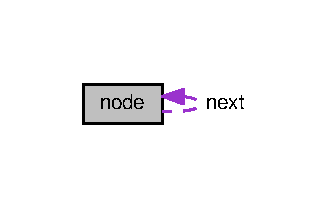
\includegraphics[width=158pt]{structnode__coll__graph}
\end{center}
\end{figure}
\index{snoop\+T@{snoop\+T}}\label{structsnoopT}
\hypertarget{group__data__structures_structsnoopT}{}
\subsubsection{struct snoop\+T}
\index{dup\+Var@{dup\+Var}}\label{structdupVar}
\hypertarget{group__data__structures_structdupVar}{}
\subsubsection{struct dup\+Var}


\subsection{Typedef Documentation}
\hypertarget{group__data__structures_ga4381025ffbd692e54189b2c679c79c99}{}\index{Data Structures and Preprocessor Macros@{Data Structures and Preprocessor Macros}!P\+A\+I\+R@{P\+A\+I\+R}}
\index{P\+A\+I\+R@{P\+A\+I\+R}!Data Structures and Preprocessor Macros@{Data Structures and Preprocessor Macros}}
\subsubsection[{P\+A\+I\+R}]{\setlength{\rightskip}{0pt plus 5cm}typedef struct {\bf vrna\+\_\+basepair\+\_\+s} {\bf P\+A\+I\+R}}\label{group__data__structures_ga4381025ffbd692e54189b2c679c79c99}


{\ttfamily \#include $<$\hyperlink{data__structures_8h}{Vienna\+R\+N\+A/data\+\_\+structures.\+h}$>$}



Old typename of \hyperlink{group__data__structures_structvrna__basepair__s}{vrna\+\_\+basepair\+\_\+s}. 

\begin{DoxyRefDesc}{Deprecated}
\item[\hyperlink{deprecated__deprecated000046}{Deprecated}]Use \hyperlink{group__data__structures_gac8c5669d3fb813cacf506489689305ce}{vrna\+\_\+basepair\+\_\+t} instead! \end{DoxyRefDesc}
\hypertarget{group__data__structures_gab1d8894b43aa84cbc50b862a73785fbc}{}\index{Data Structures and Preprocessor Macros@{Data Structures and Preprocessor Macros}!plist@{plist}}
\index{plist@{plist}!Data Structures and Preprocessor Macros@{Data Structures and Preprocessor Macros}}
\subsubsection[{plist}]{\setlength{\rightskip}{0pt plus 5cm}typedef struct {\bf vrna\+\_\+plist\+\_\+s} {\bf plist}}\label{group__data__structures_gab1d8894b43aa84cbc50b862a73785fbc}


{\ttfamily \#include $<$\hyperlink{data__structures_8h}{Vienna\+R\+N\+A/data\+\_\+structures.\+h}$>$}



Old typename of \hyperlink{group__data__structures_structvrna__plist__s}{vrna\+\_\+plist\+\_\+s}. 

\begin{DoxyRefDesc}{Deprecated}
\item[\hyperlink{deprecated__deprecated000047}{Deprecated}]Use \hyperlink{group__data__structures_ga8e4eb5e1bfc95776559575beb359af87}{vrna\+\_\+plist\+\_\+t} instead! \end{DoxyRefDesc}
\hypertarget{group__data__structures_ga8412f116a2eb07b59ade9e14ca7c5ef1}{}\index{Data Structures and Preprocessor Macros@{Data Structures and Preprocessor Macros}!cpair@{cpair}}
\index{cpair@{cpair}!Data Structures and Preprocessor Macros@{Data Structures and Preprocessor Macros}}
\subsubsection[{cpair}]{\setlength{\rightskip}{0pt plus 5cm}typedef struct {\bf vrna\+\_\+cpair\+\_\+s} {\bf cpair}}\label{group__data__structures_ga8412f116a2eb07b59ade9e14ca7c5ef1}


{\ttfamily \#include $<$\hyperlink{data__structures_8h}{Vienna\+R\+N\+A/data\+\_\+structures.\+h}$>$}



Old typename of \hyperlink{group__data__structures_structvrna__cpair__s}{vrna\+\_\+cpair\+\_\+s}. 

\begin{DoxyRefDesc}{Deprecated}
\item[\hyperlink{deprecated__deprecated000048}{Deprecated}]Use \hyperlink{group__data__structures_gae4fc91141cc69c6d8eaf1332cb991ecc}{vrna\+\_\+cpair\+\_\+t} instead! \end{DoxyRefDesc}
\hypertarget{group__data__structures_gaaacedee1f05d3d45aa6764eca51a8876}{}\index{Data Structures and Preprocessor Macros@{Data Structures and Preprocessor Macros}!sect@{sect}}
\index{sect@{sect}!Data Structures and Preprocessor Macros@{Data Structures and Preprocessor Macros}}
\subsubsection[{sect}]{\setlength{\rightskip}{0pt plus 5cm}typedef struct {\bf vrna\+\_\+sect\+\_\+s} {\bf sect}}\label{group__data__structures_gaaacedee1f05d3d45aa6764eca51a8876}


{\ttfamily \#include $<$\hyperlink{data__structures_8h}{Vienna\+R\+N\+A/data\+\_\+structures.\+h}$>$}



Old typename of \hyperlink{group__data__structures_structvrna__sect__s}{vrna\+\_\+sect\+\_\+s}. 

\begin{DoxyRefDesc}{Deprecated}
\item[\hyperlink{deprecated__deprecated000049}{Deprecated}]Use \hyperlink{group__data__structures_gacc9cdae790dac75a7024e7069c0d4400}{vrna\+\_\+sect\+\_\+t} instead! \end{DoxyRefDesc}
\hypertarget{group__data__structures_gaaeed53a7508c6ce549a98223e94b25df}{}\index{Data Structures and Preprocessor Macros@{Data Structures and Preprocessor Macros}!bond\+T@{bond\+T}}
\index{bond\+T@{bond\+T}!Data Structures and Preprocessor Macros@{Data Structures and Preprocessor Macros}}
\subsubsection[{bond\+T}]{\setlength{\rightskip}{0pt plus 5cm}typedef struct {\bf vrna\+\_\+bp\+\_\+stack\+\_\+s} {\bf bond\+T}}\label{group__data__structures_gaaeed53a7508c6ce549a98223e94b25df}


{\ttfamily \#include $<$\hyperlink{data__structures_8h}{Vienna\+R\+N\+A/data\+\_\+structures.\+h}$>$}



Old typename of \hyperlink{group__data__structures_structvrna__bp__stack__s}{vrna\+\_\+bp\+\_\+stack\+\_\+s}. 

\begin{DoxyRefDesc}{Deprecated}
\item[\hyperlink{deprecated__deprecated000050}{Deprecated}]Use \hyperlink{group__data__structures_gaa651bda42e7692f08cb603cd6834b0ee}{vrna\+\_\+bp\+\_\+stack\+\_\+t} instead! \end{DoxyRefDesc}

\hypertarget{group__utils}{}\section{Utilities}
\label{group__utils}\index{Utilities@{Utilities}}
Collaboration diagram for Utilities\+:
\nopagebreak
\begin{figure}[H]
\begin{center}
\leavevmode
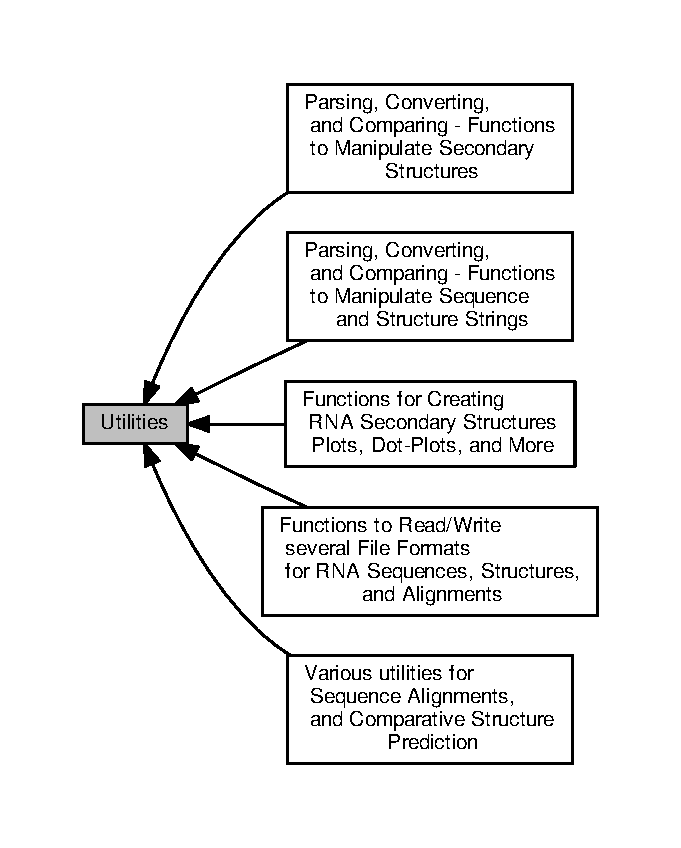
\includegraphics[width=327pt]{group__utils}
\end{center}
\end{figure}
\subsection*{Modules}
\begin{DoxyCompactItemize}
\item 
\hyperlink{group__string__utils}{Parsing, Converting, and Comparing -\/ Functions to Manipulate Sequence and Structure Strings}
\item 
\hyperlink{group__struct__utils}{Parsing, Converting, and Comparing -\/ Functions to Manipulate Secondary Structures}
\item 
\hyperlink{group__aln__utils}{Various utilities for Sequence Alignments, and Comparative Structure Prediction}
\item 
\hyperlink{group__file__utils}{Functions to Read/\+Write several File Formats for R\+N\+A Sequences, Structures, and Alignments}
\item 
\hyperlink{group__plotting__utils}{Functions for Creating R\+N\+A Secondary Structures Plots, Dot-\/\+Plots, and More}
\end{DoxyCompactItemize}
\subsection*{Files}
\begin{DoxyCompactItemize}
\item 
file \hyperlink{alphabet_8h}{alphabet.\+h}
\begin{DoxyCompactList}\small\item\em Functions to process, convert, and generally handle different nucleotide and/or base pair alphabets. \end{DoxyCompactList}\item 
file \hyperlink{utils_8h}{utils.\+h}
\begin{DoxyCompactList}\small\item\em General utility-\/ and helper-\/functions used throughout the {\itshape Vienna\+R\+N\+A} {\itshape Package}. \end{DoxyCompactList}\end{DoxyCompactItemize}
\subsection*{Macros}
\begin{DoxyCompactItemize}
\item 
\hypertarget{group__utils_gad403c9ea58f1836689404c2931419c8c}{}\#define \hyperlink{group__utils_gad403c9ea58f1836689404c2931419c8c}{V\+R\+N\+A\+\_\+\+I\+N\+P\+U\+T\+\_\+\+E\+R\+R\+O\+R}~1\+U\label{group__utils_gad403c9ea58f1836689404c2931419c8c}

\begin{DoxyCompactList}\small\item\em Output flag of \hyperlink{group__utils_ga8ef1835eb83f542396f59f0b205965e5}{get\+\_\+input\+\_\+line()}\+: {\itshape \char`\"{}\+An E\+R\+R\+O\+R has occured, maybe E\+O\+F\char`\"{}}. \end{DoxyCompactList}\item 
\hypertarget{group__utils_ga72f3c6ca5c83d2b9baed2922d19c403d}{}\#define \hyperlink{group__utils_ga72f3c6ca5c83d2b9baed2922d19c403d}{V\+R\+N\+A\+\_\+\+I\+N\+P\+U\+T\+\_\+\+Q\+U\+I\+T}~2\+U\label{group__utils_ga72f3c6ca5c83d2b9baed2922d19c403d}

\begin{DoxyCompactList}\small\item\em Output flag of \hyperlink{group__utils_ga8ef1835eb83f542396f59f0b205965e5}{get\+\_\+input\+\_\+line()}\+: {\itshape \char`\"{}the user requested quitting the program\char`\"{}}. \end{DoxyCompactList}\item 
\hypertarget{group__utils_ga8e3241b321c9c1a78a69e59e2e019a71}{}\#define \hyperlink{group__utils_ga8e3241b321c9c1a78a69e59e2e019a71}{V\+R\+N\+A\+\_\+\+I\+N\+P\+U\+T\+\_\+\+M\+I\+S\+C}~4\+U\label{group__utils_ga8e3241b321c9c1a78a69e59e2e019a71}

\begin{DoxyCompactList}\small\item\em Output flag of \hyperlink{group__utils_ga8ef1835eb83f542396f59f0b205965e5}{get\+\_\+input\+\_\+line()}\+: {\itshape \char`\"{}something was read\char`\"{}}. \end{DoxyCompactList}\item 
\#define \hyperlink{group__utils_ga2f0d8069e93d3ac54d9320d6bdb8e7e7}{V\+R\+N\+A\+\_\+\+I\+N\+P\+U\+T\+\_\+\+F\+A\+S\+T\+A\+\_\+\+H\+E\+A\+D\+E\+R}~8\+U
\begin{DoxyCompactList}\small\item\em Input/\+Output flag of \hyperlink{group__utils_ga8ef1835eb83f542396f59f0b205965e5}{get\+\_\+input\+\_\+line()}\+:~\newline
if used as input option this tells \hyperlink{group__utils_ga8ef1835eb83f542396f59f0b205965e5}{get\+\_\+input\+\_\+line()} that the data to be read should comply with the F\+A\+S\+T\+A format. \end{DoxyCompactList}\item 
\#define \hyperlink{group__utils_gac08a9df45b9721b97a47dbfe7a6e5f85}{V\+R\+N\+A\+\_\+\+I\+N\+P\+U\+T\+\_\+\+C\+O\+N\+S\+T\+R\+A\+I\+N\+T}~32\+U
\begin{DoxyCompactList}\small\item\em Input flag for \hyperlink{group__utils_ga8ef1835eb83f542396f59f0b205965e5}{get\+\_\+input\+\_\+line()}\+:~\newline
Tell \hyperlink{group__utils_ga8ef1835eb83f542396f59f0b205965e5}{get\+\_\+input\+\_\+line()} that we assume to read a structure constraint. \end{DoxyCompactList}\item 
\hypertarget{group__utils_ga086742158293217a46ae2f71bb296937}{}\#define \hyperlink{group__utils_ga086742158293217a46ae2f71bb296937}{V\+R\+N\+A\+\_\+\+I\+N\+P\+U\+T\+\_\+\+N\+O\+\_\+\+T\+R\+U\+N\+C\+A\+T\+I\+O\+N}~256\+U\label{group__utils_ga086742158293217a46ae2f71bb296937}

\begin{DoxyCompactList}\small\item\em Input switch for \hyperlink{group__utils_ga8ef1835eb83f542396f59f0b205965e5}{get\+\_\+input\+\_\+line()}\+: {\itshape \char`\"{}do not trunkate the line by eliminating white spaces at end of line\char`\"{}}. \end{DoxyCompactList}\item 
\hypertarget{group__utils_ga7a2e8c50a0c7ce82e60da1016e1367fd}{}\#define \hyperlink{group__utils_ga7a2e8c50a0c7ce82e60da1016e1367fd}{V\+R\+N\+A\+\_\+\+I\+N\+P\+U\+T\+\_\+\+N\+O\+\_\+\+R\+E\+S\+T}~512\+U\label{group__utils_ga7a2e8c50a0c7ce82e60da1016e1367fd}

\begin{DoxyCompactList}\small\item\em Input switch for \hyperlink{group__file__utils_ga8cfb7e271efc9e1f34640acb85475639}{vrna\+\_\+file\+\_\+fasta\+\_\+read\+\_\+record()}\+: {\itshape \char`\"{}do fill rest array\char`\"{}}. \end{DoxyCompactList}\item 
\hypertarget{group__utils_ga0de536599b881c787b0943a2671da476}{}\#define \hyperlink{group__utils_ga0de536599b881c787b0943a2671da476}{V\+R\+N\+A\+\_\+\+I\+N\+P\+U\+T\+\_\+\+N\+O\+\_\+\+S\+P\+A\+N}~1024\+U\label{group__utils_ga0de536599b881c787b0943a2671da476}

\begin{DoxyCompactList}\small\item\em Input switch for \hyperlink{group__file__utils_ga8cfb7e271efc9e1f34640acb85475639}{vrna\+\_\+file\+\_\+fasta\+\_\+read\+\_\+record()}\+: {\itshape \char`\"{}never allow data to span more than one line\char`\"{}}. \end{DoxyCompactList}\item 
\hypertarget{group__utils_gab4db885222b3b69608310d7c7e63e286}{}\#define \hyperlink{group__utils_gab4db885222b3b69608310d7c7e63e286}{V\+R\+N\+A\+\_\+\+I\+N\+P\+U\+T\+\_\+\+N\+O\+S\+K\+I\+P\+\_\+\+B\+L\+A\+N\+K\+\_\+\+L\+I\+N\+E\+S}~2048\+U\label{group__utils_gab4db885222b3b69608310d7c7e63e286}

\begin{DoxyCompactList}\small\item\em Input switch for \hyperlink{group__file__utils_ga8cfb7e271efc9e1f34640acb85475639}{vrna\+\_\+file\+\_\+fasta\+\_\+read\+\_\+record()}\+: {\itshape \char`\"{}do not skip empty lines\char`\"{}}. \end{DoxyCompactList}\item 
\hypertarget{group__utils_ga305474b93ccb79ae4c7754016a8ddd84}{}\#define \hyperlink{group__utils_ga305474b93ccb79ae4c7754016a8ddd84}{V\+R\+N\+A\+\_\+\+I\+N\+P\+U\+T\+\_\+\+B\+L\+A\+N\+K\+\_\+\+L\+I\+N\+E}~4096\+U\label{group__utils_ga305474b93ccb79ae4c7754016a8ddd84}

\begin{DoxyCompactList}\small\item\em Output flag for \hyperlink{group__file__utils_ga8cfb7e271efc9e1f34640acb85475639}{vrna\+\_\+file\+\_\+fasta\+\_\+read\+\_\+record()}\+: {\itshape \char`\"{}read an empty line\char`\"{}}. \end{DoxyCompactList}\item 
\hypertarget{group__utils_ga0f6311f11bed1842e3a527ab27b294c6}{}\#define \hyperlink{group__utils_ga0f6311f11bed1842e3a527ab27b294c6}{V\+R\+N\+A\+\_\+\+I\+N\+P\+U\+T\+\_\+\+N\+O\+S\+K\+I\+P\+\_\+\+C\+O\+M\+M\+E\+N\+T\+S}~128\+U\label{group__utils_ga0f6311f11bed1842e3a527ab27b294c6}

\begin{DoxyCompactList}\small\item\em Input switch for \hyperlink{group__utils_ga8ef1835eb83f542396f59f0b205965e5}{get\+\_\+input\+\_\+line()}\+: {\itshape \char`\"{}do not skip comment lines\char`\"{}}. \end{DoxyCompactList}\item 
\hypertarget{group__utils_gaf2062e0eeefffd3ed639af460b3d4fab}{}\#define \hyperlink{group__utils_gaf2062e0eeefffd3ed639af460b3d4fab}{V\+R\+N\+A\+\_\+\+I\+N\+P\+U\+T\+\_\+\+C\+O\+M\+M\+E\+N\+T}~8192\+U\label{group__utils_gaf2062e0eeefffd3ed639af460b3d4fab}

\begin{DoxyCompactList}\small\item\em Output flag for \hyperlink{group__file__utils_ga8cfb7e271efc9e1f34640acb85475639}{vrna\+\_\+file\+\_\+fasta\+\_\+read\+\_\+record()}\+: {\itshape \char`\"{}read a comment\char`\"{}}. \end{DoxyCompactList}\item 
\hypertarget{group__utils_gae0b9cd0ce090bd69b951aa73e8fa4f7d}{}\#define \hyperlink{group__utils_gae0b9cd0ce090bd69b951aa73e8fa4f7d}{M\+I\+N2}(A,  B)~((A) $<$ (B) ? (A) \+: (B))\label{group__utils_gae0b9cd0ce090bd69b951aa73e8fa4f7d}

\begin{DoxyCompactList}\small\item\em Get the minimum of two comparable values. \end{DoxyCompactList}\item 
\hypertarget{group__utils_ga33297b3679c713b0c4d897cd0fe3b122}{}\#define \hyperlink{group__utils_ga33297b3679c713b0c4d897cd0fe3b122}{M\+A\+X2}(A,  B)~((A) $>$ (B) ? (A) \+: (B))\label{group__utils_ga33297b3679c713b0c4d897cd0fe3b122}

\begin{DoxyCompactList}\small\item\em Get the maximum of two comparable values. \end{DoxyCompactList}\item 
\hypertarget{group__utils_ga721b8d5f3abef17f10293f1f7f8c958e}{}\#define \hyperlink{group__utils_ga721b8d5f3abef17f10293f1f7f8c958e}{M\+I\+N3}(A,  B,  C)~(\hyperlink{group__utils_gae0b9cd0ce090bd69b951aa73e8fa4f7d}{M\+I\+N2}(  (\hyperlink{group__utils_gae0b9cd0ce090bd69b951aa73e8fa4f7d}{M\+I\+N2}((A),(B))) ,(C)))\label{group__utils_ga721b8d5f3abef17f10293f1f7f8c958e}

\begin{DoxyCompactList}\small\item\em Get the minimum of three comparable values. \end{DoxyCompactList}\item 
\hypertarget{group__utils_ga8d577123d2e66d2b7d0bf9af6e172b93}{}\#define \hyperlink{group__utils_ga8d577123d2e66d2b7d0bf9af6e172b93}{M\+A\+X3}(A,  B,  C)~(\hyperlink{group__utils_ga33297b3679c713b0c4d897cd0fe3b122}{M\+A\+X2}(  (\hyperlink{group__utils_ga33297b3679c713b0c4d897cd0fe3b122}{M\+A\+X2}((A),(B))) ,(C)))\label{group__utils_ga8d577123d2e66d2b7d0bf9af6e172b93}

\begin{DoxyCompactList}\small\item\em Get the maximum of three comparable values. \end{DoxyCompactList}\end{DoxyCompactItemize}
\subsection*{Functions}
\begin{DoxyCompactItemize}
\item 
void $\ast$ \hyperlink{group__utils_gaf37a0979367c977edfb9da6614eebe99}{vrna\+\_\+alloc} (unsigned size)
\begin{DoxyCompactList}\small\item\em Allocate space safely. \end{DoxyCompactList}\item 
void $\ast$ \hyperlink{group__utils_ga27f4719a66c6f90d1cca3d1e6e696c6a}{vrna\+\_\+realloc} (void $\ast$p, unsigned size)
\begin{DoxyCompactList}\small\item\em Reallocate space safely. \end{DoxyCompactList}\item 
void \hyperlink{group__utils_gabb76f8f8dbd652fa4a24037cf4524373}{vrna\+\_\+message\+\_\+error} (const char message\mbox{[}$\,$\mbox{]})
\begin{DoxyCompactList}\small\item\em Die with an error message. \end{DoxyCompactList}\item 
void \hyperlink{group__utils_gafe4072406bd287c6857763dd7d2fe1f1}{vrna\+\_\+message\+\_\+warning} (const char message\mbox{[}$\,$\mbox{]})
\begin{DoxyCompactList}\small\item\em Print a warning message. \end{DoxyCompactList}\item 
\hypertarget{group__utils_ga0ad1f40ea316e5c5918695c35613027a}{}void \hyperlink{group__utils_ga0ad1f40ea316e5c5918695c35613027a}{vrna\+\_\+init\+\_\+rand} (void)\label{group__utils_ga0ad1f40ea316e5c5918695c35613027a}

\begin{DoxyCompactList}\small\item\em Initialize seed for random number generator. \end{DoxyCompactList}\item 
double \hyperlink{group__utils_ga384e256ebb295d04a14426179db0dd6e}{vrna\+\_\+urn} (void)
\begin{DoxyCompactList}\small\item\em get a random number from \mbox{[}0..1\mbox{]} \end{DoxyCompactList}\item 
int \hyperlink{group__utils_ga46111bb3747dbcf4609f0d40ae169ad9}{vrna\+\_\+int\+\_\+urn} (int from, int to)
\begin{DoxyCompactList}\small\item\em Generates a pseudo random integer in a specified range. \end{DoxyCompactList}\item 
\hypertarget{group__utils_ga4382a56d2fee9ed738364b99329edc7c}{}void \hyperlink{group__utils_ga4382a56d2fee9ed738364b99329edc7c}{vrna\+\_\+file\+\_\+copy} (F\+I\+L\+E $\ast$from, F\+I\+L\+E $\ast$to)\label{group__utils_ga4382a56d2fee9ed738364b99329edc7c}

\begin{DoxyCompactList}\small\item\em Inefficient `cp\textquotesingle{}. \end{DoxyCompactList}\item 
char $\ast$ \hyperlink{group__utils_gad3bbe8d01afb1310609cb018d5290550}{vrna\+\_\+time\+\_\+stamp} (void)
\begin{DoxyCompactList}\small\item\em Get a timestamp. \end{DoxyCompactList}\item 
char $\ast$ \hyperlink{group__utils_gabe51806d14cff0789a8c1df7dbc45b71}{get\+\_\+line} (F\+I\+L\+E $\ast$fp)
\begin{DoxyCompactList}\small\item\em Read a line of arbitrary length from a stream. \end{DoxyCompactList}\item 
unsigned int \hyperlink{group__utils_ga8ef1835eb83f542396f59f0b205965e5}{get\+\_\+input\+\_\+line} (char $\ast$$\ast$string, unsigned int options)
\item 
void \hyperlink{group__utils_gaee1dd652ca5b9e56b096963a1576f73b}{vrna\+\_\+message\+\_\+input\+\_\+seq\+\_\+simple} (void)
\begin{DoxyCompactList}\small\item\em Print a line to {\itshape stdout} that asks for an input sequence. \end{DoxyCompactList}\item 
void \hyperlink{group__utils_gaf4d194d558b0c975f269de01dea52460}{vrna\+\_\+message\+\_\+input\+\_\+seq} (const char $\ast$s)
\begin{DoxyCompactList}\small\item\em Print a line with a user defined string and a ruler to stdout. \end{DoxyCompactList}\item 
int $\ast$ \hyperlink{group__utils_ga70b180e9ea764218a82647a1cd347445}{vrna\+\_\+idx\+\_\+row\+\_\+wise} (unsigned int length)
\begin{DoxyCompactList}\small\item\em Get an index mapper array (iindx) for accessing the energy matrices, e.\+g. in partition function related functions. \end{DoxyCompactList}\item 
int $\ast$ \hyperlink{group__utils_ga89ebc69c52fa0c78c9e1974b0017746b}{vrna\+\_\+idx\+\_\+col\+\_\+wise} (unsigned int length)
\begin{DoxyCompactList}\small\item\em Get an index mapper array (indx) for accessing the energy matrices, e.\+g. in M\+F\+E related functions. \end{DoxyCompactList}\end{DoxyCompactItemize}
\subsection*{Variables}
\begin{DoxyCompactItemize}
\item 
unsigned short \hyperlink{group__utils_gaf9a866c8417afda7368bbac939ab3c47}{xsubi} \mbox{[}3\mbox{]}
\begin{DoxyCompactList}\small\item\em Current 48 bit random number. \end{DoxyCompactList}\end{DoxyCompactItemize}


\subsection{Detailed Description}


\subsection{Macro Definition Documentation}
\hypertarget{group__utils_ga2f0d8069e93d3ac54d9320d6bdb8e7e7}{}\index{Utilities@{Utilities}!V\+R\+N\+A\+\_\+\+I\+N\+P\+U\+T\+\_\+\+F\+A\+S\+T\+A\+\_\+\+H\+E\+A\+D\+E\+R@{V\+R\+N\+A\+\_\+\+I\+N\+P\+U\+T\+\_\+\+F\+A\+S\+T\+A\+\_\+\+H\+E\+A\+D\+E\+R}}
\index{V\+R\+N\+A\+\_\+\+I\+N\+P\+U\+T\+\_\+\+F\+A\+S\+T\+A\+\_\+\+H\+E\+A\+D\+E\+R@{V\+R\+N\+A\+\_\+\+I\+N\+P\+U\+T\+\_\+\+F\+A\+S\+T\+A\+\_\+\+H\+E\+A\+D\+E\+R}!Utilities@{Utilities}}
\subsubsection[{V\+R\+N\+A\+\_\+\+I\+N\+P\+U\+T\+\_\+\+F\+A\+S\+T\+A\+\_\+\+H\+E\+A\+D\+E\+R}]{\setlength{\rightskip}{0pt plus 5cm}\#define V\+R\+N\+A\+\_\+\+I\+N\+P\+U\+T\+\_\+\+F\+A\+S\+T\+A\+\_\+\+H\+E\+A\+D\+E\+R~8\+U}\label{group__utils_ga2f0d8069e93d3ac54d9320d6bdb8e7e7}


{\ttfamily \#include $<$\hyperlink{utils_8h}{Vienna\+R\+N\+A/utils.\+h}$>$}



Input/\+Output flag of \hyperlink{group__utils_ga8ef1835eb83f542396f59f0b205965e5}{get\+\_\+input\+\_\+line()}\+:~\newline
if used as input option this tells \hyperlink{group__utils_ga8ef1835eb83f542396f59f0b205965e5}{get\+\_\+input\+\_\+line()} that the data to be read should comply with the F\+A\+S\+T\+A format. 

the function will return this flag if a fasta header was read \hypertarget{group__utils_gac08a9df45b9721b97a47dbfe7a6e5f85}{}\index{Utilities@{Utilities}!V\+R\+N\+A\+\_\+\+I\+N\+P\+U\+T\+\_\+\+C\+O\+N\+S\+T\+R\+A\+I\+N\+T@{V\+R\+N\+A\+\_\+\+I\+N\+P\+U\+T\+\_\+\+C\+O\+N\+S\+T\+R\+A\+I\+N\+T}}
\index{V\+R\+N\+A\+\_\+\+I\+N\+P\+U\+T\+\_\+\+C\+O\+N\+S\+T\+R\+A\+I\+N\+T@{V\+R\+N\+A\+\_\+\+I\+N\+P\+U\+T\+\_\+\+C\+O\+N\+S\+T\+R\+A\+I\+N\+T}!Utilities@{Utilities}}
\subsubsection[{V\+R\+N\+A\+\_\+\+I\+N\+P\+U\+T\+\_\+\+C\+O\+N\+S\+T\+R\+A\+I\+N\+T}]{\setlength{\rightskip}{0pt plus 5cm}\#define V\+R\+N\+A\+\_\+\+I\+N\+P\+U\+T\+\_\+\+C\+O\+N\+S\+T\+R\+A\+I\+N\+T~32\+U}\label{group__utils_gac08a9df45b9721b97a47dbfe7a6e5f85}


{\ttfamily \#include $<$\hyperlink{utils_8h}{Vienna\+R\+N\+A/utils.\+h}$>$}



Input flag for \hyperlink{group__utils_ga8ef1835eb83f542396f59f0b205965e5}{get\+\_\+input\+\_\+line()}\+:~\newline
Tell \hyperlink{group__utils_ga8ef1835eb83f542396f59f0b205965e5}{get\+\_\+input\+\_\+line()} that we assume to read a structure constraint. 



\subsection{Function Documentation}
\hypertarget{group__utils_gaf37a0979367c977edfb9da6614eebe99}{}\index{Utilities@{Utilities}!vrna\+\_\+alloc@{vrna\+\_\+alloc}}
\index{vrna\+\_\+alloc@{vrna\+\_\+alloc}!Utilities@{Utilities}}
\subsubsection[{vrna\+\_\+alloc}]{\setlength{\rightskip}{0pt plus 5cm}void$\ast$ vrna\+\_\+alloc (
\begin{DoxyParamCaption}
\item[{unsigned}]{size}
\end{DoxyParamCaption}
)}\label{group__utils_gaf37a0979367c977edfb9da6614eebe99}


{\ttfamily \#include $<$\hyperlink{utils_8h}{Vienna\+R\+N\+A/utils.\+h}$>$}



Allocate space safely. 


\begin{DoxyParams}{Parameters}
{\em size} & The size of the memory to be allocated in bytes \\
\hline
\end{DoxyParams}
\begin{DoxyReturn}{Returns}
A pointer to the allocated memory 
\end{DoxyReturn}
\hypertarget{group__utils_ga27f4719a66c6f90d1cca3d1e6e696c6a}{}\index{Utilities@{Utilities}!vrna\+\_\+realloc@{vrna\+\_\+realloc}}
\index{vrna\+\_\+realloc@{vrna\+\_\+realloc}!Utilities@{Utilities}}
\subsubsection[{vrna\+\_\+realloc}]{\setlength{\rightskip}{0pt plus 5cm}void$\ast$ vrna\+\_\+realloc (
\begin{DoxyParamCaption}
\item[{void $\ast$}]{p, }
\item[{unsigned}]{size}
\end{DoxyParamCaption}
)}\label{group__utils_ga27f4719a66c6f90d1cca3d1e6e696c6a}


{\ttfamily \#include $<$\hyperlink{utils_8h}{Vienna\+R\+N\+A/utils.\+h}$>$}



Reallocate space safely. 


\begin{DoxyParams}{Parameters}
{\em p} & A pointer to the memory region to be reallocated \\
\hline
{\em size} & The size of the memory to be allocated in bytes \\
\hline
\end{DoxyParams}
\begin{DoxyReturn}{Returns}
A pointer to the newly allocated memory 
\end{DoxyReturn}
\hypertarget{group__utils_gabb76f8f8dbd652fa4a24037cf4524373}{}\index{Utilities@{Utilities}!vrna\+\_\+message\+\_\+error@{vrna\+\_\+message\+\_\+error}}
\index{vrna\+\_\+message\+\_\+error@{vrna\+\_\+message\+\_\+error}!Utilities@{Utilities}}
\subsubsection[{vrna\+\_\+message\+\_\+error}]{\setlength{\rightskip}{0pt plus 5cm}void vrna\+\_\+message\+\_\+error (
\begin{DoxyParamCaption}
\item[{const char}]{message\mbox{[}$\,$\mbox{]}}
\end{DoxyParamCaption}
)}\label{group__utils_gabb76f8f8dbd652fa4a24037cf4524373}


{\ttfamily \#include $<$\hyperlink{utils_8h}{Vienna\+R\+N\+A/utils.\+h}$>$}



Die with an error message. 

\begin{DoxySeeAlso}{See also}
\hyperlink{group__utils_gafe4072406bd287c6857763dd7d2fe1f1}{vrna\+\_\+message\+\_\+warning()} 
\end{DoxySeeAlso}

\begin{DoxyParams}{Parameters}
{\em message} & The error message to be printed before exiting with \textquotesingle{}F\+A\+I\+L\+U\+R\+E\textquotesingle{} \\
\hline
\end{DoxyParams}
\hypertarget{group__utils_gafe4072406bd287c6857763dd7d2fe1f1}{}\index{Utilities@{Utilities}!vrna\+\_\+message\+\_\+warning@{vrna\+\_\+message\+\_\+warning}}
\index{vrna\+\_\+message\+\_\+warning@{vrna\+\_\+message\+\_\+warning}!Utilities@{Utilities}}
\subsubsection[{vrna\+\_\+message\+\_\+warning}]{\setlength{\rightskip}{0pt plus 5cm}void vrna\+\_\+message\+\_\+warning (
\begin{DoxyParamCaption}
\item[{const char}]{message\mbox{[}$\,$\mbox{]}}
\end{DoxyParamCaption}
)}\label{group__utils_gafe4072406bd287c6857763dd7d2fe1f1}


{\ttfamily \#include $<$\hyperlink{utils_8h}{Vienna\+R\+N\+A/utils.\+h}$>$}



Print a warning message. 

Print a warning message to {\itshape stderr} 


\begin{DoxyParams}{Parameters}
{\em message} & The warning message \\
\hline
\end{DoxyParams}
\hypertarget{group__utils_ga384e256ebb295d04a14426179db0dd6e}{}\index{Utilities@{Utilities}!vrna\+\_\+urn@{vrna\+\_\+urn}}
\index{vrna\+\_\+urn@{vrna\+\_\+urn}!Utilities@{Utilities}}
\subsubsection[{vrna\+\_\+urn}]{\setlength{\rightskip}{0pt plus 5cm}double vrna\+\_\+urn (
\begin{DoxyParamCaption}
\item[{void}]{}
\end{DoxyParamCaption}
)}\label{group__utils_ga384e256ebb295d04a14426179db0dd6e}


{\ttfamily \#include $<$\hyperlink{utils_8h}{Vienna\+R\+N\+A/utils.\+h}$>$}



get a random number from \mbox{[}0..1\mbox{]} 

\begin{DoxySeeAlso}{See also}
\hyperlink{group__utils_ga46111bb3747dbcf4609f0d40ae169ad9}{vrna\+\_\+int\+\_\+urn()}, \hyperlink{group__utils_ga0ad1f40ea316e5c5918695c35613027a}{vrna\+\_\+init\+\_\+rand()} 
\end{DoxySeeAlso}
\begin{DoxyNote}{Note}
Usually implemented by calling {\itshape erand48()}. 
\end{DoxyNote}
\begin{DoxyReturn}{Returns}
A random number in range \mbox{[}0..1\mbox{]} 
\end{DoxyReturn}
\hypertarget{group__utils_ga46111bb3747dbcf4609f0d40ae169ad9}{}\index{Utilities@{Utilities}!vrna\+\_\+int\+\_\+urn@{vrna\+\_\+int\+\_\+urn}}
\index{vrna\+\_\+int\+\_\+urn@{vrna\+\_\+int\+\_\+urn}!Utilities@{Utilities}}
\subsubsection[{vrna\+\_\+int\+\_\+urn}]{\setlength{\rightskip}{0pt plus 5cm}int vrna\+\_\+int\+\_\+urn (
\begin{DoxyParamCaption}
\item[{int}]{from, }
\item[{int}]{to}
\end{DoxyParamCaption}
)}\label{group__utils_ga46111bb3747dbcf4609f0d40ae169ad9}


{\ttfamily \#include $<$\hyperlink{utils_8h}{Vienna\+R\+N\+A/utils.\+h}$>$}



Generates a pseudo random integer in a specified range. 

\begin{DoxySeeAlso}{See also}
\hyperlink{group__utils_ga384e256ebb295d04a14426179db0dd6e}{vrna\+\_\+urn()}, \hyperlink{group__utils_ga0ad1f40ea316e5c5918695c35613027a}{vrna\+\_\+init\+\_\+rand()} 
\end{DoxySeeAlso}

\begin{DoxyParams}{Parameters}
{\em from} & The first number in range \\
\hline
{\em to} & The last number in range \\
\hline
\end{DoxyParams}
\begin{DoxyReturn}{Returns}
A pseudo random number in range \mbox{[}from, to\mbox{]} 
\end{DoxyReturn}
\hypertarget{group__utils_gad3bbe8d01afb1310609cb018d5290550}{}\index{Utilities@{Utilities}!vrna\+\_\+time\+\_\+stamp@{vrna\+\_\+time\+\_\+stamp}}
\index{vrna\+\_\+time\+\_\+stamp@{vrna\+\_\+time\+\_\+stamp}!Utilities@{Utilities}}
\subsubsection[{vrna\+\_\+time\+\_\+stamp}]{\setlength{\rightskip}{0pt plus 5cm}char$\ast$ vrna\+\_\+time\+\_\+stamp (
\begin{DoxyParamCaption}
\item[{void}]{}
\end{DoxyParamCaption}
)}\label{group__utils_gad3bbe8d01afb1310609cb018d5290550}


{\ttfamily \#include $<$\hyperlink{utils_8h}{Vienna\+R\+N\+A/utils.\+h}$>$}



Get a timestamp. 

Returns a string containing the current date in the format \begin{DoxyVerb}Fri Mar 19 21:10:57 1993 \end{DoxyVerb}


\begin{DoxyReturn}{Returns}
A string containing the timestamp 
\end{DoxyReturn}
\hypertarget{group__utils_gabe51806d14cff0789a8c1df7dbc45b71}{}\index{Utilities@{Utilities}!get\+\_\+line@{get\+\_\+line}}
\index{get\+\_\+line@{get\+\_\+line}!Utilities@{Utilities}}
\subsubsection[{get\+\_\+line}]{\setlength{\rightskip}{0pt plus 5cm}char$\ast$ get\+\_\+line (
\begin{DoxyParamCaption}
\item[{F\+I\+L\+E $\ast$}]{fp}
\end{DoxyParamCaption}
)}\label{group__utils_gabe51806d14cff0789a8c1df7dbc45b71}


{\ttfamily \#include $<$\hyperlink{utils_8h}{Vienna\+R\+N\+A/utils.\+h}$>$}



Read a line of arbitrary length from a stream. 

Returns a pointer to the resulting string. The necessary memory is allocated and should be released using {\itshape free()} when the string is no longer needed.


\begin{DoxyParams}{Parameters}
{\em fp} & A file pointer to the stream where the function should read from \\
\hline
\end{DoxyParams}
\begin{DoxyReturn}{Returns}
A pointer to the resulting string 
\end{DoxyReturn}
\hypertarget{group__utils_ga8ef1835eb83f542396f59f0b205965e5}{}\index{Utilities@{Utilities}!get\+\_\+input\+\_\+line@{get\+\_\+input\+\_\+line}}
\index{get\+\_\+input\+\_\+line@{get\+\_\+input\+\_\+line}!Utilities@{Utilities}}
\subsubsection[{get\+\_\+input\+\_\+line}]{\setlength{\rightskip}{0pt plus 5cm}unsigned int get\+\_\+input\+\_\+line (
\begin{DoxyParamCaption}
\item[{char $\ast$$\ast$}]{string, }
\item[{unsigned int}]{options}
\end{DoxyParamCaption}
)}\label{group__utils_ga8ef1835eb83f542396f59f0b205965e5}


{\ttfamily \#include $<$\hyperlink{utils_8h}{Vienna\+R\+N\+A/utils.\+h}$>$}

Retrieve a line from \textquotesingle{}stdin\textquotesingle{} savely while skipping comment characters and other features This function returns the type of input it has read if recognized. An option argument allows to switch between different reading modes.~\newline
Currently available options are\+:~\newline
\#\+V\+R\+N\+A\+\_\+\+I\+N\+P\+U\+T\+\_\+\+N\+O\+P\+R\+I\+N\+T\+\_\+\+C\+O\+M\+M\+E\+N\+T\+S, \hyperlink{group__utils_ga0f6311f11bed1842e3a527ab27b294c6}{V\+R\+N\+A\+\_\+\+I\+N\+P\+U\+T\+\_\+\+N\+O\+S\+K\+I\+P\+\_\+\+C\+O\+M\+M\+E\+N\+T\+S}, \#\+V\+R\+N\+A\+\_\+\+I\+N\+P\+U\+T\+\_\+\+N\+O\+E\+L\+I\+M\+\_\+\+W\+S\+\_\+\+S\+U\+F\+F\+I\+X

pass a collection of options as one value like this\+: \begin{DoxyVerb}get_input_line(string, option_1 | option_2 | option_n) \end{DoxyVerb}


If the function recognizes the type of input, it will report it in the return value. It also reports if a user defined \textquotesingle{}quit\textquotesingle{} command (@-\/sign on \textquotesingle{}stdin\textquotesingle{}) was given. Possible return values are\+:~\newline
\hyperlink{group__utils_ga2f0d8069e93d3ac54d9320d6bdb8e7e7}{V\+R\+N\+A\+\_\+\+I\+N\+P\+U\+T\+\_\+\+F\+A\+S\+T\+A\+\_\+\+H\+E\+A\+D\+E\+R}, \hyperlink{group__utils_gad403c9ea58f1836689404c2931419c8c}{V\+R\+N\+A\+\_\+\+I\+N\+P\+U\+T\+\_\+\+E\+R\+R\+O\+R}, \hyperlink{group__utils_ga8e3241b321c9c1a78a69e59e2e019a71}{V\+R\+N\+A\+\_\+\+I\+N\+P\+U\+T\+\_\+\+M\+I\+S\+C}, \hyperlink{group__utils_ga72f3c6ca5c83d2b9baed2922d19c403d}{V\+R\+N\+A\+\_\+\+I\+N\+P\+U\+T\+\_\+\+Q\+U\+I\+T}


\begin{DoxyParams}{Parameters}
{\em string} & A pointer to the character array that contains the line read \\
\hline
{\em options} & A collection of options for switching the functions behavior \\
\hline
\end{DoxyParams}
\begin{DoxyReturn}{Returns}
A flag with information about what has been read 
\end{DoxyReturn}
\hypertarget{group__utils_gaee1dd652ca5b9e56b096963a1576f73b}{}\index{Utilities@{Utilities}!vrna\+\_\+message\+\_\+input\+\_\+seq\+\_\+simple@{vrna\+\_\+message\+\_\+input\+\_\+seq\+\_\+simple}}
\index{vrna\+\_\+message\+\_\+input\+\_\+seq\+\_\+simple@{vrna\+\_\+message\+\_\+input\+\_\+seq\+\_\+simple}!Utilities@{Utilities}}
\subsubsection[{vrna\+\_\+message\+\_\+input\+\_\+seq\+\_\+simple}]{\setlength{\rightskip}{0pt plus 5cm}void vrna\+\_\+message\+\_\+input\+\_\+seq\+\_\+simple (
\begin{DoxyParamCaption}
\item[{void}]{}
\end{DoxyParamCaption}
)}\label{group__utils_gaee1dd652ca5b9e56b096963a1576f73b}


{\ttfamily \#include $<$\hyperlink{utils_8h}{Vienna\+R\+N\+A/utils.\+h}$>$}



Print a line to {\itshape stdout} that asks for an input sequence. 

There will also be a ruler (scale line) printed that helps orientation of the sequence positions \hypertarget{group__utils_gaf4d194d558b0c975f269de01dea52460}{}\index{Utilities@{Utilities}!vrna\+\_\+message\+\_\+input\+\_\+seq@{vrna\+\_\+message\+\_\+input\+\_\+seq}}
\index{vrna\+\_\+message\+\_\+input\+\_\+seq@{vrna\+\_\+message\+\_\+input\+\_\+seq}!Utilities@{Utilities}}
\subsubsection[{vrna\+\_\+message\+\_\+input\+\_\+seq}]{\setlength{\rightskip}{0pt plus 5cm}void vrna\+\_\+message\+\_\+input\+\_\+seq (
\begin{DoxyParamCaption}
\item[{const char $\ast$}]{s}
\end{DoxyParamCaption}
)}\label{group__utils_gaf4d194d558b0c975f269de01dea52460}


{\ttfamily \#include $<$\hyperlink{utils_8h}{Vienna\+R\+N\+A/utils.\+h}$>$}



Print a line with a user defined string and a ruler to stdout. 

(usually this is used to ask for user input) There will also be a ruler (scale line) printed that helps orientation of the sequence positions


\begin{DoxyParams}{Parameters}
{\em s} & A user defined string that will be printed to stdout \\
\hline
\end{DoxyParams}
\hypertarget{group__utils_ga70b180e9ea764218a82647a1cd347445}{}\index{Utilities@{Utilities}!vrna\+\_\+idx\+\_\+row\+\_\+wise@{vrna\+\_\+idx\+\_\+row\+\_\+wise}}
\index{vrna\+\_\+idx\+\_\+row\+\_\+wise@{vrna\+\_\+idx\+\_\+row\+\_\+wise}!Utilities@{Utilities}}
\subsubsection[{vrna\+\_\+idx\+\_\+row\+\_\+wise}]{\setlength{\rightskip}{0pt plus 5cm}int$\ast$ vrna\+\_\+idx\+\_\+row\+\_\+wise (
\begin{DoxyParamCaption}
\item[{unsigned int}]{length}
\end{DoxyParamCaption}
)}\label{group__utils_ga70b180e9ea764218a82647a1cd347445}


{\ttfamily \#include $<$\hyperlink{utils_8h}{Vienna\+R\+N\+A/utils.\+h}$>$}



Get an index mapper array (iindx) for accessing the energy matrices, e.\+g. in partition function related functions. 

Access of a position \char`\"{}(i,j)\char`\"{} is then accomplished by using\begin{DoxyVerb}(i,j) ~ iindx[i]-j \end{DoxyVerb}
 This function is necessary as most of the two-\/dimensional energy matrices are actually one-\/dimensional arrays throughout the Vienna\+R\+N\+A Package

Consult the implemented code to find out about the mapping formula ;)

\begin{DoxySeeAlso}{See also}
\hyperlink{group__utils_ga89ebc69c52fa0c78c9e1974b0017746b}{vrna\+\_\+idx\+\_\+col\+\_\+wise()} 
\end{DoxySeeAlso}

\begin{DoxyParams}{Parameters}
{\em length} & The length of the R\+N\+A sequence \\
\hline
\end{DoxyParams}
\begin{DoxyReturn}{Returns}
The mapper array 
\end{DoxyReturn}
\hypertarget{group__utils_ga89ebc69c52fa0c78c9e1974b0017746b}{}\index{Utilities@{Utilities}!vrna\+\_\+idx\+\_\+col\+\_\+wise@{vrna\+\_\+idx\+\_\+col\+\_\+wise}}
\index{vrna\+\_\+idx\+\_\+col\+\_\+wise@{vrna\+\_\+idx\+\_\+col\+\_\+wise}!Utilities@{Utilities}}
\subsubsection[{vrna\+\_\+idx\+\_\+col\+\_\+wise}]{\setlength{\rightskip}{0pt plus 5cm}int$\ast$ vrna\+\_\+idx\+\_\+col\+\_\+wise (
\begin{DoxyParamCaption}
\item[{unsigned int}]{length}
\end{DoxyParamCaption}
)}\label{group__utils_ga89ebc69c52fa0c78c9e1974b0017746b}


{\ttfamily \#include $<$\hyperlink{utils_8h}{Vienna\+R\+N\+A/utils.\+h}$>$}



Get an index mapper array (indx) for accessing the energy matrices, e.\+g. in M\+F\+E related functions. 

Access of a position \char`\"{}(i,j)\char`\"{} is then accomplished by using\begin{DoxyVerb}(i,j) ~ indx[j]+i \end{DoxyVerb}
 This function is necessary as most of the two-\/dimensional energy matrices are actually one-\/dimensional arrays throughout the Vienna\+R\+N\+A\+Package

Consult the implemented code to find out about the mapping formula ;)

\begin{DoxySeeAlso}{See also}
\hyperlink{group__utils_ga70b180e9ea764218a82647a1cd347445}{vrna\+\_\+idx\+\_\+row\+\_\+wise()} 
\end{DoxySeeAlso}

\begin{DoxyParams}{Parameters}
{\em length} & The length of the R\+N\+A sequence \\
\hline
\end{DoxyParams}
\begin{DoxyReturn}{Returns}
The mapper array 
\end{DoxyReturn}


\subsection{Variable Documentation}
\hypertarget{group__utils_gaf9a866c8417afda7368bbac939ab3c47}{}\index{Utilities@{Utilities}!xsubi@{xsubi}}
\index{xsubi@{xsubi}!Utilities@{Utilities}}
\subsubsection[{xsubi}]{\setlength{\rightskip}{0pt plus 5cm}unsigned short xsubi\mbox{[}3\mbox{]}}\label{group__utils_gaf9a866c8417afda7368bbac939ab3c47}


{\ttfamily \#include $<$\hyperlink{utils_8h}{Vienna\+R\+N\+A/utils.\+h}$>$}



Current 48 bit random number. 

This variable is used by \hyperlink{group__utils_ga384e256ebb295d04a14426179db0dd6e}{vrna\+\_\+urn()}. These should be set to some random number seeds before the first call to \hyperlink{group__utils_ga384e256ebb295d04a14426179db0dd6e}{vrna\+\_\+urn()}.

\begin{DoxySeeAlso}{See also}
\hyperlink{group__utils_ga384e256ebb295d04a14426179db0dd6e}{vrna\+\_\+urn()} 
\end{DoxySeeAlso}

\hypertarget{group__mfe__fold}{}\section{Computing Minimum Free Energy (M\+F\+E) Structures}
\label{group__mfe__fold}\index{Computing Minimum Free Energy (\+M\+F\+E) Structures@{Computing Minimum Free Energy (\+M\+F\+E) Structures}}


This section covers all functions and variables related to the calculation of minimum free energy (M\+F\+E) structures.  


Collaboration diagram for Computing Minimum Free Energy (M\+F\+E) Structures\+:
\nopagebreak
\begin{figure}[H]
\begin{center}
\leavevmode
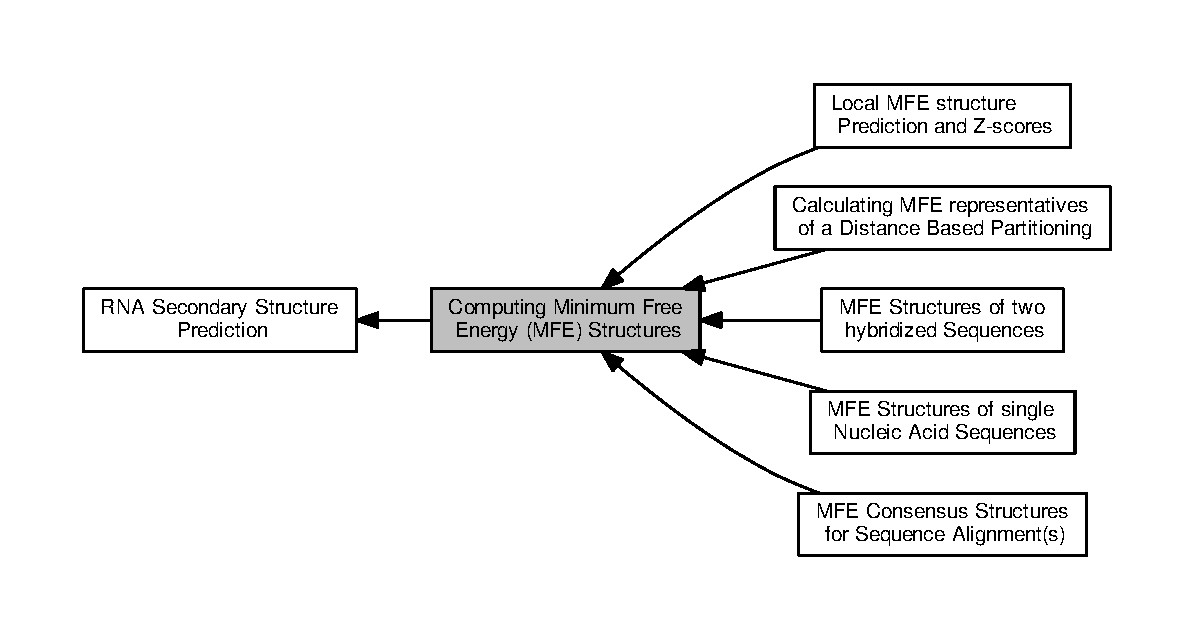
\includegraphics[width=350pt]{group__mfe__fold}
\end{center}
\end{figure}
\subsection*{Modules}
\begin{DoxyCompactItemize}
\item 
\hyperlink{group__mfe__fold__single}{M\+F\+E Structures of single Nucleic Acid Sequences}
\begin{DoxyCompactList}\small\item\em This module contains all functions and variables related to the calculation of global minimum free energy structures for single sequences. \end{DoxyCompactList}\item 
\hyperlink{group__mfe__cofold}{M\+F\+E Structures of two hybridized Sequences}
\item 
\hyperlink{group__consensus__mfe__fold}{M\+F\+E Consensus Structures for Sequence Alignment(s)}
\item 
\hyperlink{group__local__mfe__fold}{Local M\+F\+E structure Prediction and Z-\/scores}
\item 
\hyperlink{group__kl__neighborhood__mfe}{Calculating M\+F\+E representatives of a Distance Based Partitioning}
\begin{DoxyCompactList}\small\item\em Compute the minimum free energy (M\+F\+E) and secondary structures for a partitioning of the secondary structure space according to the base pair distance to two fixed reference structures basepair distance to two fixed reference structures. \end{DoxyCompactList}\end{DoxyCompactItemize}
\subsection*{Functions}
\begin{DoxyCompactItemize}
\item 
float \hyperlink{group__mfe__fold_gabd3b147371ccf25c577f88bbbaf159fd}{vrna\+\_\+mfe} (\hyperlink{group__fold__compound_ga1b0cef17fd40466cef5968eaeeff6166}{vrna\+\_\+fold\+\_\+compound\+\_\+t} $\ast$vc, char $\ast$structure)
\begin{DoxyCompactList}\small\item\em Compute minimum free energy and an appropriate secondary structure of an R\+N\+A sequence, or R\+N\+A sequence alignment. \end{DoxyCompactList}\end{DoxyCompactItemize}


\subsection{Detailed Description}
This section covers all functions and variables related to the calculation of minimum free energy (M\+F\+E) structures. 

The library provides a fast dynamic programming minimum free energy folding algorithm as described in \cite{zuker:1981}. All relevant parts that directly implement the \char`\"{}\+Zuker \& Stiegler\char`\"{} algorithm for single sequences are described in this section.

Folding of circular R\+N\+A sequences is handled as a post-\/processing step of the forward recursions. See \cite{hofacker:2006} for further details.

Nevertheless, the R\+N\+Alib also provides interfaces for the prediction of consensus M\+F\+E structures of sequence alignments, M\+F\+E structure for two hybridized sequences, local optimal structures and many more. For those more specialized variants of M\+F\+E folding routines, please consult the appropriate subsections (Modules) as listed above. 

\subsection{Function Documentation}
\hypertarget{group__mfe__fold_gabd3b147371ccf25c577f88bbbaf159fd}{}\index{Computing Minimum Free Energy (\+M\+F\+E) Structures@{Computing Minimum Free Energy (\+M\+F\+E) Structures}!vrna\+\_\+mfe@{vrna\+\_\+mfe}}
\index{vrna\+\_\+mfe@{vrna\+\_\+mfe}!Computing Minimum Free Energy (\+M\+F\+E) Structures@{Computing Minimum Free Energy (\+M\+F\+E) Structures}}
\subsubsection[{vrna\+\_\+mfe}]{\setlength{\rightskip}{0pt plus 5cm}float vrna\+\_\+mfe (
\begin{DoxyParamCaption}
\item[{{\bf vrna\+\_\+fold\+\_\+compound\+\_\+t} $\ast$}]{vc, }
\item[{char $\ast$}]{structure}
\end{DoxyParamCaption}
)}\label{group__mfe__fold_gabd3b147371ccf25c577f88bbbaf159fd}


{\ttfamily \#include $<$\hyperlink{mfe_8h}{Vienna\+R\+N\+A/mfe.\+h}$>$}



Compute minimum free energy and an appropriate secondary structure of an R\+N\+A sequence, or R\+N\+A sequence alignment. 

Depending on the type of the provided \hyperlink{group__fold__compound_ga1b0cef17fd40466cef5968eaeeff6166}{vrna\+\_\+fold\+\_\+compound\+\_\+t}, this function predicts the M\+F\+E for a single sequence, or a corresponding averaged M\+F\+E for a sequence alignment. If backtracking is activated, it also constructs the corresponding secondary structure, or consensus structure. Therefore, the second parameter, {\itshape structure}, has to point to an allocated block of memory with a size of at least $\mathrm{strlen}(\mathrm{sequence})+1$ to store the backtracked M\+F\+E structure. (For consensus structures, this is the length of the alignment + 1. If {\ttfamily N\+U\+L\+L} is passed, no backtracking will be performed.

\begin{DoxyNote}{Note}
This function is polymorphic. It accepts \hyperlink{group__fold__compound_ga1b0cef17fd40466cef5968eaeeff6166}{vrna\+\_\+fold\+\_\+compound\+\_\+t} of type \hyperlink{group__fold__compound_gga01a4ff86fa71deaaa5d1abbd95a1447da1608d3aa78905fc39e0d25a624ac9512}{V\+R\+N\+A\+\_\+\+V\+C\+\_\+\+T\+Y\+P\+E\+\_\+\+S\+I\+N\+G\+L\+E}, and \hyperlink{group__fold__compound_gga01a4ff86fa71deaaa5d1abbd95a1447da056345f1bcfe7cd595d1fd437c05246d}{V\+R\+N\+A\+\_\+\+V\+C\+\_\+\+T\+Y\+P\+E\+\_\+\+A\+L\+I\+G\+N\+M\+E\+N\+T}.
\end{DoxyNote}
\begin{DoxySeeAlso}{See also}
\hyperlink{group__fold__compound_ga1b0cef17fd40466cef5968eaeeff6166}{vrna\+\_\+fold\+\_\+compound\+\_\+t}, \hyperlink{group__fold__compound_ga6601d994ba32b11511b36f68b08403be}{vrna\+\_\+fold\+\_\+compound()}, \hyperlink{group__mfe__fold__single_gae7ca49ffb3086f145da36c964a7cec64}{vrna\+\_\+fold()}, \hyperlink{group__mfe__fold__single_gaa0f5bf321038f404b36a6147bdae4154}{vrna\+\_\+circfold()}, \hyperlink{group__fold__compound_gad6bacc816af274922b13d947f708aa0c}{vrna\+\_\+fold\+\_\+compound\+\_\+comparative()}, \hyperlink{group__consensus__mfe__fold_ga02098d0c8790f9a37fbef6ad0cfc705c}{vrna\+\_\+alifold()}, \hyperlink{group__consensus__mfe__fold_ga01ce2cff93ea44c4f4254760ca2bd16c}{vrna\+\_\+circalifold()}
\end{DoxySeeAlso}

\begin{DoxyParams}{Parameters}
{\em vc} & fold compound \\
\hline
{\em structure} & A pointer to the character array where the secondary structure in dot-\/bracket notation will be written to (Maybe N\+U\+L\+L)\\
\hline
\end{DoxyParams}
\begin{DoxyReturn}{Returns}
the minimum free energy (M\+F\+E) in kcal/mol 
\end{DoxyReturn}

\hypertarget{group__pf__fold}{}\section{Computing Partition Functions and Pair Probabilities}
\label{group__pf__fold}\index{Computing Partition Functions and Pair Probabilities@{Computing Partition Functions and Pair Probabilities}}


This section provides information about all functions and variables related to the calculation of the partition function and base pair probabilities.  


Collaboration diagram for Computing Partition Functions and Pair Probabilities\+:
\nopagebreak
\begin{figure}[H]
\begin{center}
\leavevmode
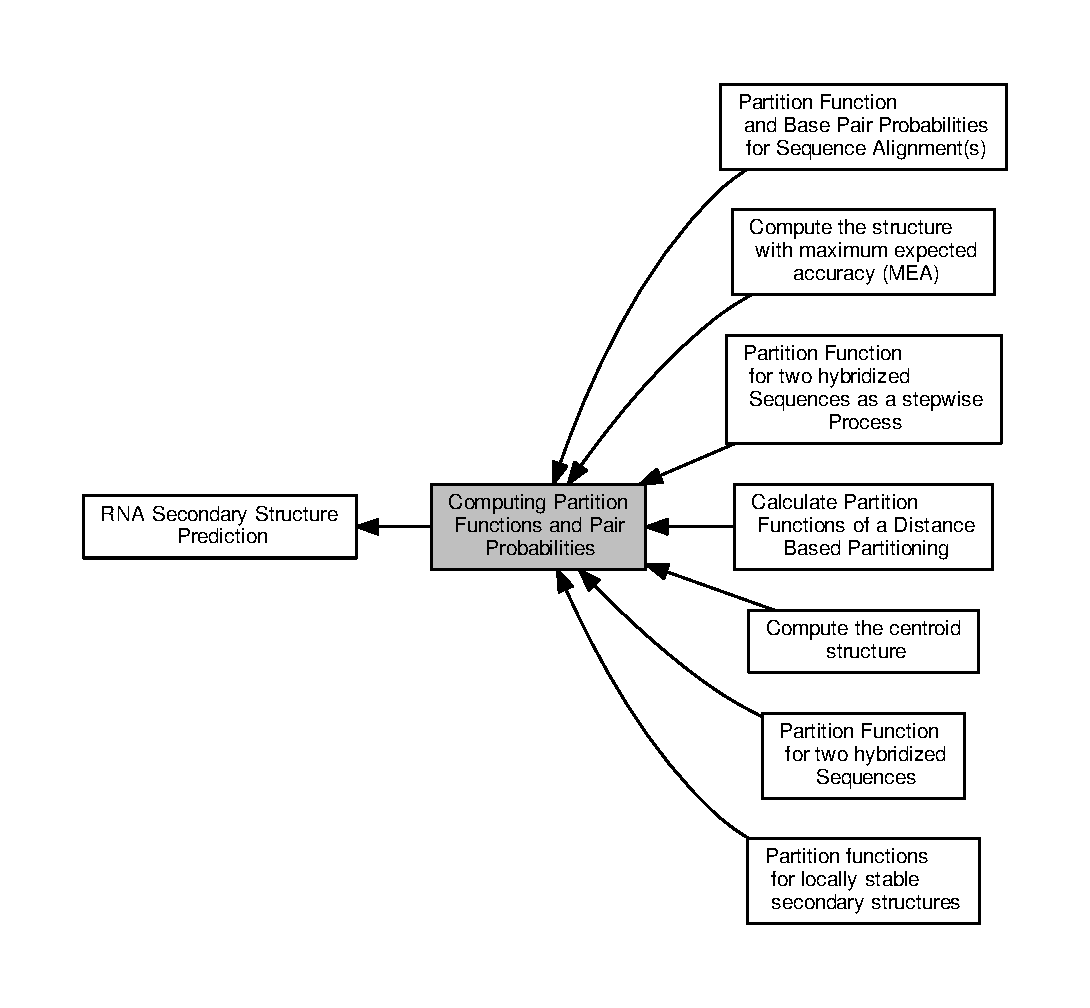
\includegraphics[width=350pt]{group__pf__fold}
\end{center}
\end{figure}
\subsection*{Modules}
\begin{DoxyCompactItemize}
\item 
\hyperlink{group__mea__fold}{Compute the structure with maximum expected accuracy (\+M\+E\+A)}
\item 
\hyperlink{group__centroid__fold}{Compute the centroid structure}
\item 
\hyperlink{group__pf__cofold}{Partition Function for two hybridized Sequences}
\begin{DoxyCompactList}\small\item\em Partition Function Cofolding. \end{DoxyCompactList}\item 
\hyperlink{group__up__cofold}{Partition Function for two hybridized Sequences as a stepwise Process}
\begin{DoxyCompactList}\small\item\em Partition Function Cofolding as a stepwise process. \end{DoxyCompactList}\item 
\hyperlink{group__consensus__pf__fold}{Partition Function and Base Pair Probabilities for Sequence Alignment(s)}
\item 
\hyperlink{group__local__pf__fold}{Partition functions for locally stable secondary structures}
\item 
\hyperlink{group__kl__neighborhood__pf}{Calculate Partition Functions of a Distance Based Partitioning}
\begin{DoxyCompactList}\small\item\em Compute the partition function and stochastically sample secondary structures for a partitioning of the secondary structure space according to the base pair distance to two fixed reference structures. \end{DoxyCompactList}\end{DoxyCompactItemize}
\subsection*{Files}
\begin{DoxyCompactItemize}
\item 
file \hyperlink{boltzmann__sampling_8h}{boltzmann\+\_\+sampling.\+h}
\begin{DoxyCompactList}\small\item\em Boltzmann Sampling of secondary structures from the ensemble. \end{DoxyCompactList}\item 
file \hyperlink{part__func_8h}{part\+\_\+func.\+h}
\begin{DoxyCompactList}\small\item\em Partition function of single R\+N\+A sequences. \end{DoxyCompactList}\end{DoxyCompactItemize}
\subsection*{Functions}
\begin{DoxyCompactItemize}
\item 
float \hyperlink{group__pf__fold_ga29e256d688ad221b78d37f427e0e99bc}{vrna\+\_\+pf} (\hyperlink{group__fold__compound_ga1b0cef17fd40466cef5968eaeeff6166}{vrna\+\_\+fold\+\_\+compound\+\_\+t} $\ast$vc, char $\ast$structure)
\begin{DoxyCompactList}\small\item\em Compute the partition function $Q$ for a given R\+N\+A sequence, or sequence alignment. \end{DoxyCompactList}\item 
float \hyperlink{group__pf__fold_ga59935ba485ac90f0efb5a38e2962d879}{vrna\+\_\+pf\+\_\+fold} (const char $\ast$seq, char $\ast$structure, \hyperlink{group__data__structures_ga8e4eb5e1bfc95776559575beb359af87}{vrna\+\_\+plist\+\_\+t} $\ast$$\ast$pl)
\begin{DoxyCompactList}\small\item\em Compute Partition function $Q$ (and base pair probabilities) for an R\+N\+A sequence using a comparative method. \end{DoxyCompactList}\item 
float \hyperlink{group__pf__fold_ga6dc133fce577fc0370986f3a3301cd10}{vrna\+\_\+pf\+\_\+circfold} (const char $\ast$seq, char $\ast$structure, \hyperlink{group__data__structures_ga8e4eb5e1bfc95776559575beb359af87}{vrna\+\_\+plist\+\_\+t} $\ast$$\ast$pl)
\begin{DoxyCompactList}\small\item\em Compute Partition function $Q$ (and base pair probabilities) for a circular R\+N\+A sequences using a comparative method. \end{DoxyCompactList}\item 
double \hyperlink{group__pf__fold_gad3f0c240512e6d43e2e4d4c2076021f5}{vrna\+\_\+mean\+\_\+bp\+\_\+distance\+\_\+pr} (int length, \hyperlink{group__data__structures_ga31125aeace516926bf7f251f759b6126}{F\+L\+T\+\_\+\+O\+R\+\_\+\+D\+B\+L} $\ast$\hyperlink{fold__vars_8h_ac98ec419070aee6831b44e5c700f090f}{pr})
\begin{DoxyCompactList}\small\item\em Get the mean base pair distance in the thermodynamic ensemble from a probability matrix. \end{DoxyCompactList}\item 
double \hyperlink{group__pf__fold_gaa6b8983b559b9ef4b2e1b31113ea317b}{vrna\+\_\+mean\+\_\+bp\+\_\+distance} (\hyperlink{group__fold__compound_ga1b0cef17fd40466cef5968eaeeff6166}{vrna\+\_\+fold\+\_\+compound\+\_\+t} $\ast$vc)
\begin{DoxyCompactList}\small\item\em Get the mean base pair distance in the thermodynamic ensemble. \end{DoxyCompactList}\item 
\hyperlink{group__data__structures_ga8e4eb5e1bfc95776559575beb359af87}{vrna\+\_\+plist\+\_\+t} $\ast$ \hyperlink{group__pf__fold_ga26e3cc2eb127a35625572e9275c24ee4}{vrna\+\_\+stack\+\_\+prob} (\hyperlink{group__fold__compound_ga1b0cef17fd40466cef5968eaeeff6166}{vrna\+\_\+fold\+\_\+compound\+\_\+t} $\ast$vc, double cutoff)
\begin{DoxyCompactList}\small\item\em Compute stacking probabilities. \end{DoxyCompactList}\item 
float \hyperlink{group__pf__fold_gac4f95bee734b2563a3d6e9932117ebdf}{pf\+\_\+fold\+\_\+par} (const char $\ast$sequence, char $\ast$structure, \hyperlink{group__energy__parameters_ga01d8b92fe734df8d79a6169482c7d8d8}{vrna\+\_\+exp\+\_\+param\+\_\+t} $\ast$parameters, int calculate\+\_\+bppm, int is\+\_\+constrained, int is\+\_\+circular)
\begin{DoxyCompactList}\small\item\em Compute the partition function $Q$ for a given R\+N\+A sequence. \end{DoxyCompactList}\item 
float \hyperlink{group__pf__fold_gadc3db3d98742427e7001a7fd36ef28c2}{pf\+\_\+fold} (const char $\ast$sequence, char $\ast$structure)
\begin{DoxyCompactList}\small\item\em Compute the partition function $Q$ of an R\+N\+A sequence. \end{DoxyCompactList}\item 
float \hyperlink{group__pf__fold_ga819ce5fca8984004ac81c4a3b04cb735}{pf\+\_\+circ\+\_\+fold} (const char $\ast$sequence, char $\ast$structure)
\begin{DoxyCompactList}\small\item\em Compute the partition function of a circular R\+N\+A sequence. \end{DoxyCompactList}\item 
void \hyperlink{group__pf__fold_gae73db3f49a94f0f72e067ecd12681dbd}{free\+\_\+pf\+\_\+arrays} (void)
\begin{DoxyCompactList}\small\item\em Free arrays for the partition function recursions. \end{DoxyCompactList}\item 
void \hyperlink{group__pf__fold_ga384e927890f9c034ff09fa66da102d28}{update\+\_\+pf\+\_\+params} (int length)
\begin{DoxyCompactList}\small\item\em Recalculate energy parameters. \end{DoxyCompactList}\item 
void \hyperlink{group__pf__fold_gaafe2d1b21f5418b123b088aa395e827d}{update\+\_\+pf\+\_\+params\+\_\+par} (int length, \hyperlink{group__energy__parameters_ga01d8b92fe734df8d79a6169482c7d8d8}{vrna\+\_\+exp\+\_\+param\+\_\+t} $\ast$parameters)
\begin{DoxyCompactList}\small\item\em Recalculate energy parameters. \end{DoxyCompactList}\item 
\hyperlink{group__data__structures_ga31125aeace516926bf7f251f759b6126}{F\+L\+T\+\_\+\+O\+R\+\_\+\+D\+B\+L} $\ast$ \hyperlink{group__pf__fold_gac5ac7ee281aae1c5cc5898a841178073}{export\+\_\+bppm} (void)
\begin{DoxyCompactList}\small\item\em Get a pointer to the base pair probability array

Accessing the base pair probabilities for a pair (i,j) is achieved by. \end{DoxyCompactList}\item 
int \hyperlink{group__pf__fold_ga42faebdfce6f070c5f89adfc8427525c}{get\+\_\+pf\+\_\+arrays} (short $\ast$$\ast$S\+\_\+p, short $\ast$$\ast$S1\+\_\+p, char $\ast$$\ast$ptype\+\_\+p, \hyperlink{group__data__structures_ga31125aeace516926bf7f251f759b6126}{F\+L\+T\+\_\+\+O\+R\+\_\+\+D\+B\+L} $\ast$$\ast$qb\+\_\+p, \hyperlink{group__data__structures_ga31125aeace516926bf7f251f759b6126}{F\+L\+T\+\_\+\+O\+R\+\_\+\+D\+B\+L} $\ast$$\ast$qm\+\_\+p, \hyperlink{group__data__structures_ga31125aeace516926bf7f251f759b6126}{F\+L\+T\+\_\+\+O\+R\+\_\+\+D\+B\+L} $\ast$$\ast$q1k\+\_\+p, \hyperlink{group__data__structures_ga31125aeace516926bf7f251f759b6126}{F\+L\+T\+\_\+\+O\+R\+\_\+\+D\+B\+L} $\ast$$\ast$qln\+\_\+p)
\begin{DoxyCompactList}\small\item\em Get the pointers to (almost) all relavant computation arrays used in partition function computation. \end{DoxyCompactList}\item 
double \hyperlink{group__pf__fold_ga79cbc375af65f11609feb6b055269e7d}{mean\+\_\+bp\+\_\+distance} (int length)
\begin{DoxyCompactList}\small\item\em Get the mean base pair distance of the last partition function computation. \end{DoxyCompactList}\item 
double \hyperlink{group__pf__fold_gad5ba36cef8d01cf4244cc09b9bf1ce1d}{mean\+\_\+bp\+\_\+distance\+\_\+pr} (int length, \hyperlink{group__data__structures_ga31125aeace516926bf7f251f759b6126}{F\+L\+T\+\_\+\+O\+R\+\_\+\+D\+B\+L} $\ast$\hyperlink{fold__vars_8h_ac98ec419070aee6831b44e5c700f090f}{pr})
\begin{DoxyCompactList}\small\item\em Get the mean base pair distance in the thermodynamic ensemble. \end{DoxyCompactList}\item 
\hyperlink{group__data__structures_ga8e4eb5e1bfc95776559575beb359af87}{vrna\+\_\+plist\+\_\+t} $\ast$ \hyperlink{group__pf__fold_gaa3bf26a0ee2e9f2225afbaee44a37264}{vrna\+\_\+plist\+\_\+from\+\_\+probs} (\hyperlink{group__fold__compound_ga1b0cef17fd40466cef5968eaeeff6166}{vrna\+\_\+fold\+\_\+compound\+\_\+t} $\ast$vc, double cut\+\_\+off)
\begin{DoxyCompactList}\small\item\em Create a \hyperlink{group__data__structures_ga8e4eb5e1bfc95776559575beb359af87}{vrna\+\_\+plist\+\_\+t} from base pair probability matrix. \end{DoxyCompactList}\item 
void \hyperlink{group__pf__fold_gacfdacc119b749bccf939de445afea07b}{assign\+\_\+plist\+\_\+from\+\_\+pr} (\hyperlink{group__data__structures_ga8e4eb5e1bfc95776559575beb359af87}{vrna\+\_\+plist\+\_\+t} $\ast$$\ast$pl, \hyperlink{group__data__structures_ga31125aeace516926bf7f251f759b6126}{F\+L\+T\+\_\+\+O\+R\+\_\+\+D\+B\+L} $\ast$probs, int length, double cutoff)
\begin{DoxyCompactList}\small\item\em Create a vrna\+\_\+plist\+\_\+t from a probability matrix. \end{DoxyCompactList}\end{DoxyCompactItemize}


\subsection{Detailed Description}
This section provides information about all functions and variables related to the calculation of the partition function and base pair probabilities. 

Instead of the minimum free energy structure the partition function of all possible structures and from that the pairing probability for every possible pair can be calculated, using a dynamic programming algorithm as described in \cite{mccaskill:1990}. 

\subsection{Function Documentation}
\hypertarget{group__pf__fold_ga29e256d688ad221b78d37f427e0e99bc}{}\index{Computing Partition Functions and Pair Probabilities@{Computing Partition Functions and Pair Probabilities}!vrna\+\_\+pf@{vrna\+\_\+pf}}
\index{vrna\+\_\+pf@{vrna\+\_\+pf}!Computing Partition Functions and Pair Probabilities@{Computing Partition Functions and Pair Probabilities}}
\subsubsection[{vrna\+\_\+pf}]{\setlength{\rightskip}{0pt plus 5cm}float vrna\+\_\+pf (
\begin{DoxyParamCaption}
\item[{{\bf vrna\+\_\+fold\+\_\+compound\+\_\+t} $\ast$}]{vc, }
\item[{char $\ast$}]{structure}
\end{DoxyParamCaption}
)}\label{group__pf__fold_ga29e256d688ad221b78d37f427e0e99bc}


{\ttfamily \#include $<$\hyperlink{part__func_8h}{Vienna\+R\+N\+A/part\+\_\+func.\+h}$>$}



Compute the partition function $Q$ for a given R\+N\+A sequence, or sequence alignment. 

If {\itshape structure} is not a N\+U\+L\+L pointer on input, it contains on return a string consisting of the letters \char`\"{} . , $\vert$ \{ \} ( ) \char`\"{} denoting bases that are essentially unpaired, weakly paired, strongly paired without preference, weakly upstream (downstream) paired, or strongly up-\/ (down-\/)stream paired bases, respectively. If the parameter calculate\+\_\+bppm is set to 0 base pairing probabilities will not be computed (saving C\+P\+U time), otherwise after calculations took place \hyperlink{fold__vars_8h_ac98ec419070aee6831b44e5c700f090f}{pr} will contain the probability that bases {\itshape i} and {\itshape j} pair.

\begin{DoxyNote}{Note}
This function is polymorphic. It accepts \hyperlink{group__fold__compound_ga1b0cef17fd40466cef5968eaeeff6166}{vrna\+\_\+fold\+\_\+compound\+\_\+t} of type \hyperlink{group__fold__compound_gga01a4ff86fa71deaaa5d1abbd95a1447da1608d3aa78905fc39e0d25a624ac9512}{V\+R\+N\+A\+\_\+\+V\+C\+\_\+\+T\+Y\+P\+E\+\_\+\+S\+I\+N\+G\+L\+E}, and \hyperlink{group__fold__compound_gga01a4ff86fa71deaaa5d1abbd95a1447da056345f1bcfe7cd595d1fd437c05246d}{V\+R\+N\+A\+\_\+\+V\+C\+\_\+\+T\+Y\+P\+E\+\_\+\+A\+L\+I\+G\+N\+M\+E\+N\+T}.
\end{DoxyNote}
\begin{DoxySeeAlso}{See also}
\hyperlink{group__fold__compound_ga1b0cef17fd40466cef5968eaeeff6166}{vrna\+\_\+fold\+\_\+compound\+\_\+t}, \hyperlink{group__fold__compound_ga6601d994ba32b11511b36f68b08403be}{vrna\+\_\+fold\+\_\+compound()}, \hyperlink{group__pf__fold_ga59935ba485ac90f0efb5a38e2962d879}{vrna\+\_\+pf\+\_\+fold()}, \hyperlink{group__pf__fold_ga6dc133fce577fc0370986f3a3301cd10}{vrna\+\_\+pf\+\_\+circfold()}, \hyperlink{group__fold__compound_gad6bacc816af274922b13d947f708aa0c}{vrna\+\_\+fold\+\_\+compound\+\_\+comparative()}, \hyperlink{group__consensus__pf__fold_gaef750636c70e597a85ee139197a4350d}{vrna\+\_\+pf\+\_\+alifold()}, \hyperlink{group__consensus__pf__fold_ga017209394a4c1e68d96cd47e61d16d25}{vrna\+\_\+pf\+\_\+circalifold()}, \hyperlink{group__struct__utils_ga0c28c410a5ab22d6ab9c77a84e8d5b44}{vrna\+\_\+db\+\_\+from\+\_\+probs()}, \hyperlink{group__energy__parameters_gab1f3016f96aa96bff020cdd904605afa}{vrna\+\_\+exp\+\_\+params()}, \hyperlink{group__aln__utils_gaf6421a1318586c59fea6a127ed9f65f3}{vrna\+\_\+aln\+\_\+pinfo()}
\end{DoxySeeAlso}

\begin{DoxyParams}[1]{Parameters}
\mbox{\tt in,out}  & {\em vc} & The fold compound data structure \\
\hline
\mbox{\tt in,out}  & {\em structure} & A pointer to the character array where position-\/wise pairing propensity will be stored. (Maybe N\+U\+L\+L) \\
\hline
\end{DoxyParams}
\begin{DoxyReturn}{Returns}
The Gibbs free energy of the ensemble ( $G = -RT \cdot \log(Q) $) in kcal/mol 
\end{DoxyReturn}
\hypertarget{group__pf__fold_ga59935ba485ac90f0efb5a38e2962d879}{}\index{Computing Partition Functions and Pair Probabilities@{Computing Partition Functions and Pair Probabilities}!vrna\+\_\+pf\+\_\+fold@{vrna\+\_\+pf\+\_\+fold}}
\index{vrna\+\_\+pf\+\_\+fold@{vrna\+\_\+pf\+\_\+fold}!Computing Partition Functions and Pair Probabilities@{Computing Partition Functions and Pair Probabilities}}
\subsubsection[{vrna\+\_\+pf\+\_\+fold}]{\setlength{\rightskip}{0pt plus 5cm}float vrna\+\_\+pf\+\_\+fold (
\begin{DoxyParamCaption}
\item[{const char $\ast$}]{seq, }
\item[{char $\ast$}]{structure, }
\item[{{\bf vrna\+\_\+plist\+\_\+t} $\ast$$\ast$}]{pl}
\end{DoxyParamCaption}
)}\label{group__pf__fold_ga59935ba485ac90f0efb5a38e2962d879}


{\ttfamily \#include $<$\hyperlink{part__func_8h}{Vienna\+R\+N\+A/part\+\_\+func.\+h}$>$}



Compute Partition function $Q$ (and base pair probabilities) for an R\+N\+A sequence using a comparative method. 

This simplified interface to \hyperlink{group__pf__fold_ga29e256d688ad221b78d37f427e0e99bc}{vrna\+\_\+pf()} computes the partition function and, if required, base pair probabilities for an R\+N\+A sequence using default options. Memory required for dynamic programming (D\+P) matrices will be allocated and free\textquotesingle{}d on-\/the-\/fly. Hence, after return of this function, the recursively filled matrices are not available any more for any post-\/processing.

\begin{DoxyNote}{Note}
In case you want to use the filled D\+P matrices for any subsequent post-\/processing step, or you require other conditions than specified by the default model details, use \hyperlink{group__pf__fold_ga29e256d688ad221b78d37f427e0e99bc}{vrna\+\_\+pf()}, and the data structure \hyperlink{group__fold__compound_ga1b0cef17fd40466cef5968eaeeff6166}{vrna\+\_\+fold\+\_\+compound\+\_\+t} instead.
\end{DoxyNote}
\begin{DoxySeeAlso}{See also}
\hyperlink{group__pf__fold_ga6dc133fce577fc0370986f3a3301cd10}{vrna\+\_\+pf\+\_\+circfold()}, \hyperlink{group__pf__fold_ga29e256d688ad221b78d37f427e0e99bc}{vrna\+\_\+pf()}, \hyperlink{group__fold__compound_ga6601d994ba32b11511b36f68b08403be}{vrna\+\_\+fold\+\_\+compound()}, \hyperlink{group__fold__compound_ga1b0cef17fd40466cef5968eaeeff6166}{vrna\+\_\+fold\+\_\+compound\+\_\+t}
\end{DoxySeeAlso}

\begin{DoxyParams}{Parameters}
{\em sequences} & R\+N\+A sequence \\
\hline
{\em structure} & A pointer to the character array where position-\/wise pairing propensity will be stored. (Maybe N\+U\+L\+L) \\
\hline
{\em pl} & A pointer to a list of \hyperlink{group__data__structures_ga8e4eb5e1bfc95776559575beb359af87}{vrna\+\_\+plist\+\_\+t} to store pairing probabilities (Maybe N\+U\+L\+L) \\
\hline
\end{DoxyParams}
\begin{DoxyReturn}{Returns}
The Gibbs free energy of the ensemble ( $G = -RT \cdot \log(Q) $) in kcal/mol 
\end{DoxyReturn}
\hypertarget{group__pf__fold_ga6dc133fce577fc0370986f3a3301cd10}{}\index{Computing Partition Functions and Pair Probabilities@{Computing Partition Functions and Pair Probabilities}!vrna\+\_\+pf\+\_\+circfold@{vrna\+\_\+pf\+\_\+circfold}}
\index{vrna\+\_\+pf\+\_\+circfold@{vrna\+\_\+pf\+\_\+circfold}!Computing Partition Functions and Pair Probabilities@{Computing Partition Functions and Pair Probabilities}}
\subsubsection[{vrna\+\_\+pf\+\_\+circfold}]{\setlength{\rightskip}{0pt plus 5cm}float vrna\+\_\+pf\+\_\+circfold (
\begin{DoxyParamCaption}
\item[{const char $\ast$}]{seq, }
\item[{char $\ast$}]{structure, }
\item[{{\bf vrna\+\_\+plist\+\_\+t} $\ast$$\ast$}]{pl}
\end{DoxyParamCaption}
)}\label{group__pf__fold_ga6dc133fce577fc0370986f3a3301cd10}


{\ttfamily \#include $<$\hyperlink{part__func_8h}{Vienna\+R\+N\+A/part\+\_\+func.\+h}$>$}



Compute Partition function $Q$ (and base pair probabilities) for a circular R\+N\+A sequences using a comparative method. 

This simplified interface to \hyperlink{group__pf__fold_ga29e256d688ad221b78d37f427e0e99bc}{vrna\+\_\+pf()} computes the partition function and, if required, base pair probabilities for a circular R\+N\+A sequence using default options. Memory required for dynamic programming (D\+P) matrices will be allocated and free\textquotesingle{}d on-\/the-\/fly. Hence, after return of this function, the recursively filled matrices are not available any more for any post-\/processing.

\begin{DoxyNote}{Note}
In case you want to use the filled D\+P matrices for any subsequent post-\/processing step, or you require other conditions than specified by the default model details, use \hyperlink{group__pf__fold_ga29e256d688ad221b78d37f427e0e99bc}{vrna\+\_\+pf()}, and the data structure \hyperlink{group__fold__compound_ga1b0cef17fd40466cef5968eaeeff6166}{vrna\+\_\+fold\+\_\+compound\+\_\+t} instead.
\end{DoxyNote}
Folding of circular R\+N\+A sequences is handled as a post-\/processing step of the forward recursions. See \cite{hofacker:2006} for further details.

\begin{DoxySeeAlso}{See also}
\hyperlink{group__pf__fold_ga59935ba485ac90f0efb5a38e2962d879}{vrna\+\_\+pf\+\_\+fold()}, \hyperlink{group__pf__fold_ga29e256d688ad221b78d37f427e0e99bc}{vrna\+\_\+pf()}, \hyperlink{group__fold__compound_ga6601d994ba32b11511b36f68b08403be}{vrna\+\_\+fold\+\_\+compound()}, \hyperlink{group__fold__compound_ga1b0cef17fd40466cef5968eaeeff6166}{vrna\+\_\+fold\+\_\+compound\+\_\+t}
\end{DoxySeeAlso}

\begin{DoxyParams}{Parameters}
{\em sequences} & A circular R\+N\+A sequence \\
\hline
{\em structure} & A pointer to the character array where position-\/wise pairing propensity will be stored. (Maybe N\+U\+L\+L) \\
\hline
{\em pl} & A pointer to a list of \hyperlink{group__data__structures_ga8e4eb5e1bfc95776559575beb359af87}{vrna\+\_\+plist\+\_\+t} to store pairing probabilities (Maybe N\+U\+L\+L) \\
\hline
\end{DoxyParams}
\begin{DoxyReturn}{Returns}
The Gibbs free energy of the ensemble ( $G = -RT \cdot \log(Q) $) in kcal/mol 
\end{DoxyReturn}
\hypertarget{group__pf__fold_gad3f0c240512e6d43e2e4d4c2076021f5}{}\index{Computing Partition Functions and Pair Probabilities@{Computing Partition Functions and Pair Probabilities}!vrna\+\_\+mean\+\_\+bp\+\_\+distance\+\_\+pr@{vrna\+\_\+mean\+\_\+bp\+\_\+distance\+\_\+pr}}
\index{vrna\+\_\+mean\+\_\+bp\+\_\+distance\+\_\+pr@{vrna\+\_\+mean\+\_\+bp\+\_\+distance\+\_\+pr}!Computing Partition Functions and Pair Probabilities@{Computing Partition Functions and Pair Probabilities}}
\subsubsection[{vrna\+\_\+mean\+\_\+bp\+\_\+distance\+\_\+pr}]{\setlength{\rightskip}{0pt plus 5cm}double vrna\+\_\+mean\+\_\+bp\+\_\+distance\+\_\+pr (
\begin{DoxyParamCaption}
\item[{int}]{length, }
\item[{{\bf F\+L\+T\+\_\+\+O\+R\+\_\+\+D\+B\+L} $\ast$}]{pr}
\end{DoxyParamCaption}
)}\label{group__pf__fold_gad3f0c240512e6d43e2e4d4c2076021f5}


{\ttfamily \#include $<$\hyperlink{part__func_8h}{Vienna\+R\+N\+A/part\+\_\+func.\+h}$>$}



Get the mean base pair distance in the thermodynamic ensemble from a probability matrix. 

$<d> = \sum_{a,b} p_a p_b d(S_a,S_b)$~\newline
this can be computed from the pair probs $p_ij$ as~\newline
 $<d> = \sum_{ij} p_{ij}(1-p_{ij})$


\begin{DoxyParams}{Parameters}
{\em length} & The length of the sequence \\
\hline
{\em pr} & The matrix containing the base pair probabilities \\
\hline
\end{DoxyParams}
\begin{DoxyReturn}{Returns}
The mean pair distance of the structure ensemble 
\end{DoxyReturn}
\hypertarget{group__pf__fold_gaa6b8983b559b9ef4b2e1b31113ea317b}{}\index{Computing Partition Functions and Pair Probabilities@{Computing Partition Functions and Pair Probabilities}!vrna\+\_\+mean\+\_\+bp\+\_\+distance@{vrna\+\_\+mean\+\_\+bp\+\_\+distance}}
\index{vrna\+\_\+mean\+\_\+bp\+\_\+distance@{vrna\+\_\+mean\+\_\+bp\+\_\+distance}!Computing Partition Functions and Pair Probabilities@{Computing Partition Functions and Pair Probabilities}}
\subsubsection[{vrna\+\_\+mean\+\_\+bp\+\_\+distance}]{\setlength{\rightskip}{0pt plus 5cm}double vrna\+\_\+mean\+\_\+bp\+\_\+distance (
\begin{DoxyParamCaption}
\item[{{\bf vrna\+\_\+fold\+\_\+compound\+\_\+t} $\ast$}]{vc}
\end{DoxyParamCaption}
)}\label{group__pf__fold_gaa6b8983b559b9ef4b2e1b31113ea317b}


{\ttfamily \#include $<$\hyperlink{part__func_8h}{Vienna\+R\+N\+A/part\+\_\+func.\+h}$>$}



Get the mean base pair distance in the thermodynamic ensemble. 

$<d> = \sum_{a,b} p_a p_b d(S_a,S_b)$~\newline
this can be computed from the pair probs $p_ij$ as~\newline
 $<d> = \sum_{ij} p_{ij}(1-p_{ij})$


\begin{DoxyParams}{Parameters}
{\em vc} & The fold compound data structure \\
\hline
\end{DoxyParams}
\begin{DoxyReturn}{Returns}
The mean pair distance of the structure ensemble 
\end{DoxyReturn}
\hypertarget{group__pf__fold_ga26e3cc2eb127a35625572e9275c24ee4}{}\index{Computing Partition Functions and Pair Probabilities@{Computing Partition Functions and Pair Probabilities}!vrna\+\_\+stack\+\_\+prob@{vrna\+\_\+stack\+\_\+prob}}
\index{vrna\+\_\+stack\+\_\+prob@{vrna\+\_\+stack\+\_\+prob}!Computing Partition Functions and Pair Probabilities@{Computing Partition Functions and Pair Probabilities}}
\subsubsection[{vrna\+\_\+stack\+\_\+prob}]{\setlength{\rightskip}{0pt plus 5cm}{\bf vrna\+\_\+plist\+\_\+t}$\ast$ vrna\+\_\+stack\+\_\+prob (
\begin{DoxyParamCaption}
\item[{{\bf vrna\+\_\+fold\+\_\+compound\+\_\+t} $\ast$}]{vc, }
\item[{double}]{cutoff}
\end{DoxyParamCaption}
)}\label{group__pf__fold_ga26e3cc2eb127a35625572e9275c24ee4}


{\ttfamily \#include $<$\hyperlink{part__func_8h}{Vienna\+R\+N\+A/part\+\_\+func.\+h}$>$}



Compute stacking probabilities. 

For each possible base pair $(i,j)$, compute the probability of a stack $(i,j)$, $(i+1, j-1)$.


\begin{DoxyParams}{Parameters}
{\em vc} & The fold compound data structure with precomputed base pair probabilities \\
\hline
{\em cutoff} & A cutoff value that limits the output to stacks with $ p > \textrm{cutoff} $. \\
\hline
\end{DoxyParams}
\begin{DoxyReturn}{Returns}
A list of stacks with enclosing base pair $(i,j)$ and probabiltiy $ p $ 
\end{DoxyReturn}
\hypertarget{group__pf__fold_gac4f95bee734b2563a3d6e9932117ebdf}{}\index{Computing Partition Functions and Pair Probabilities@{Computing Partition Functions and Pair Probabilities}!pf\+\_\+fold\+\_\+par@{pf\+\_\+fold\+\_\+par}}
\index{pf\+\_\+fold\+\_\+par@{pf\+\_\+fold\+\_\+par}!Computing Partition Functions and Pair Probabilities@{Computing Partition Functions and Pair Probabilities}}
\subsubsection[{pf\+\_\+fold\+\_\+par}]{\setlength{\rightskip}{0pt plus 5cm}float pf\+\_\+fold\+\_\+par (
\begin{DoxyParamCaption}
\item[{const char $\ast$}]{sequence, }
\item[{char $\ast$}]{structure, }
\item[{{\bf vrna\+\_\+exp\+\_\+param\+\_\+t} $\ast$}]{parameters, }
\item[{int}]{calculate\+\_\+bppm, }
\item[{int}]{is\+\_\+constrained, }
\item[{int}]{is\+\_\+circular}
\end{DoxyParamCaption}
)}\label{group__pf__fold_gac4f95bee734b2563a3d6e9932117ebdf}


{\ttfamily \#include $<$\hyperlink{part__func_8h}{Vienna\+R\+N\+A/part\+\_\+func.\+h}$>$}



Compute the partition function $Q$ for a given R\+N\+A sequence. 

If {\itshape structure} is not a N\+U\+L\+L pointer on input, it contains on return a string consisting of the letters \char`\"{} . , $\vert$ \{ \} ( ) \char`\"{} denoting bases that are essentially unpaired, weakly paired, strongly paired without preference, weakly upstream (downstream) paired, or strongly up-\/ (down-\/)stream paired bases, respectively. If \hyperlink{fold__vars_8h_a0afc287c2464866d94858c39175154af}{fold\+\_\+constrained} is not 0, the {\itshape structure} string is interpreted on input as a list of constraints for the folding. The character \char`\"{}x\char`\"{} marks bases that must be unpaired, matching brackets \char`\"{} ( ) \char`\"{} denote base pairs, all other characters are ignored. Any pairs conflicting with the constraint will be forbidden. This is usually sufficient to ensure the constraints are honored. If the parameter calculate\+\_\+bppm is set to 0 base pairing probabilities will not be computed (saving C\+P\+U time), otherwise after calculations took place \hyperlink{fold__vars_8h_ac98ec419070aee6831b44e5c700f090f}{pr} will contain the probability that bases {\itshape i} and {\itshape j} pair.

\begin{DoxyRefDesc}{Deprecated}
\item[\hyperlink{deprecated__deprecated000101}{Deprecated}]Use \hyperlink{group__pf__fold_ga29e256d688ad221b78d37f427e0e99bc}{vrna\+\_\+pf()} instead\end{DoxyRefDesc}


\begin{DoxyNote}{Note}
The global array \hyperlink{fold__vars_8h_ac98ec419070aee6831b44e5c700f090f}{pr} is deprecated and the user who wants the calculated base pair probabilities for further computations is advised to use the function \hyperlink{group__pf__fold_gac5ac7ee281aae1c5cc5898a841178073}{export\+\_\+bppm()} 
\end{DoxyNote}
\begin{DoxyPostcond}{Postcondition}
After successful run the hidden folding matrices are filled with the appropriate Boltzmann factors. Depending on whether the global variable \hyperlink{group__model__details_gad512b5dd4dbec60faccfe137bb474489}{do\+\_\+backtrack} was set the base pair probabilities are already computed and may be accessed for further usage via the \hyperlink{group__pf__fold_gac5ac7ee281aae1c5cc5898a841178073}{export\+\_\+bppm()} function. A call of \hyperlink{group__pf__fold_gae73db3f49a94f0f72e067ecd12681dbd}{free\+\_\+pf\+\_\+arrays()} will free all memory allocated by this function. Successive calls will first free previously allocated memory before starting the computation. 
\end{DoxyPostcond}
\begin{DoxySeeAlso}{See also}
\hyperlink{group__pf__fold_ga29e256d688ad221b78d37f427e0e99bc}{vrna\+\_\+pf()}, \hyperlink{group__struct__utils_ga129d81c4a1ead793c5b2311333e03dfa}{bppm\+\_\+to\+\_\+structure()}, \hyperlink{group__pf__fold_gac5ac7ee281aae1c5cc5898a841178073}{export\+\_\+bppm()}, \hyperlink{group__energy__parameters_gab1f3016f96aa96bff020cdd904605afa}{vrna\+\_\+exp\+\_\+params()}, \hyperlink{group__pf__fold_gae73db3f49a94f0f72e067ecd12681dbd}{free\+\_\+pf\+\_\+arrays()} 
\end{DoxySeeAlso}

\begin{DoxyParams}[1]{Parameters}
\mbox{\tt in}  & {\em sequence} & The R\+N\+A sequence input \\
\hline
\mbox{\tt in,out}  & {\em structure} & A pointer to a char array where a base pair probability information can be stored in a pseudo-\/dot-\/bracket notation (may be N\+U\+L\+L, too) \\
\hline
\mbox{\tt in}  & {\em parameters} & Data structure containing the precalculated Boltzmann factors \\
\hline
\mbox{\tt in}  & {\em calculate\+\_\+bppm} & Switch to Base pair probability calculations on/off (0==off) \\
\hline
\mbox{\tt in}  & {\em is\+\_\+constrained} & Switch to indicate that a structure contraint is passed via the structure argument (0==off) \\
\hline
\mbox{\tt in}  & {\em is\+\_\+circular} & Switch to (de-\/)activate postprocessing steps in case R\+N\+A sequence is circular (0==off) \\
\hline
\end{DoxyParams}
\begin{DoxyReturn}{Returns}
The Gibbs free energy of the ensemble ( $G = -RT \cdot \log(Q) $) in kcal/mol 
\end{DoxyReturn}
\hypertarget{group__pf__fold_gadc3db3d98742427e7001a7fd36ef28c2}{}\index{Computing Partition Functions and Pair Probabilities@{Computing Partition Functions and Pair Probabilities}!pf\+\_\+fold@{pf\+\_\+fold}}
\index{pf\+\_\+fold@{pf\+\_\+fold}!Computing Partition Functions and Pair Probabilities@{Computing Partition Functions and Pair Probabilities}}
\subsubsection[{pf\+\_\+fold}]{\setlength{\rightskip}{0pt plus 5cm}float pf\+\_\+fold (
\begin{DoxyParamCaption}
\item[{const char $\ast$}]{sequence, }
\item[{char $\ast$}]{structure}
\end{DoxyParamCaption}
)}\label{group__pf__fold_gadc3db3d98742427e7001a7fd36ef28c2}


{\ttfamily \#include $<$\hyperlink{part__func_8h}{Vienna\+R\+N\+A/part\+\_\+func.\+h}$>$}



Compute the partition function $Q$ of an R\+N\+A sequence. 

If {\itshape structure} is not a N\+U\+L\+L pointer on input, it contains on return a string consisting of the letters \char`\"{} . , $\vert$ \{ \} ( ) \char`\"{} denoting bases that are essentially unpaired, weakly paired, strongly paired without preference, weakly upstream (downstream) paired, or strongly up-\/ (down-\/)stream paired bases, respectively. If \hyperlink{fold__vars_8h_a0afc287c2464866d94858c39175154af}{fold\+\_\+constrained} is not 0, the {\itshape structure} string is interpreted on input as a list of constraints for the folding. The character \char`\"{}x\char`\"{} marks bases that must be unpaired, matching brackets \char`\"{} ( ) \char`\"{} denote base pairs, all other characters are ignored. Any pairs conflicting with the constraint will be forbidden. This is usually sufficient to ensure the constraints are honored. If \hyperlink{group__model__details_gad512b5dd4dbec60faccfe137bb474489}{do\+\_\+backtrack} has been set to 0 base pairing probabilities will not be computed (saving C\+P\+U time), otherwise \hyperlink{fold__vars_8h_ac98ec419070aee6831b44e5c700f090f}{pr} will contain the probability that bases {\itshape i} and {\itshape j} pair.

\begin{DoxyNote}{Note}
The global array \hyperlink{fold__vars_8h_ac98ec419070aee6831b44e5c700f090f}{pr} is deprecated and the user who wants the calculated base pair probabilities for further computations is advised to use the function \hyperlink{group__pf__fold_gac5ac7ee281aae1c5cc5898a841178073}{export\+\_\+bppm()}. 

{\bfseries Open\+M\+P\+:} This function is not entirely threadsafe. While the recursions are working on their own copies of data the model details for the recursions are determined from the global settings just before entering the recursions. Consider using \hyperlink{group__pf__fold_gac4f95bee734b2563a3d6e9932117ebdf}{pf\+\_\+fold\+\_\+par()} for a really threadsafe implementation. 
\end{DoxyNote}
\begin{DoxyPrecond}{Precondition}
This function takes its model details from the global variables provided in {\itshape R\+N\+Alib} 
\end{DoxyPrecond}
\begin{DoxyPostcond}{Postcondition}
After successful run the hidden folding matrices are filled with the appropriate Boltzmann factors. Depending on whether the global variable \hyperlink{group__model__details_gad512b5dd4dbec60faccfe137bb474489}{do\+\_\+backtrack} was set the base pair probabilities are already computed and may be accessed for further usage via the \hyperlink{group__pf__fold_gac5ac7ee281aae1c5cc5898a841178073}{export\+\_\+bppm()} function. A call of \hyperlink{group__pf__fold_gae73db3f49a94f0f72e067ecd12681dbd}{free\+\_\+pf\+\_\+arrays()} will free all memory allocated by this function. Successive calls will first free previously allocated memory before starting the computation. 
\end{DoxyPostcond}
\begin{DoxySeeAlso}{See also}
\hyperlink{group__pf__fold_gac4f95bee734b2563a3d6e9932117ebdf}{pf\+\_\+fold\+\_\+par()}, \hyperlink{group__pf__fold_ga819ce5fca8984004ac81c4a3b04cb735}{pf\+\_\+circ\+\_\+fold()}, \hyperlink{group__struct__utils_ga129d81c4a1ead793c5b2311333e03dfa}{bppm\+\_\+to\+\_\+structure()}, \hyperlink{group__pf__fold_gac5ac7ee281aae1c5cc5898a841178073}{export\+\_\+bppm()} 
\end{DoxySeeAlso}

\begin{DoxyParams}{Parameters}
{\em sequence} & The R\+N\+A sequence input \\
\hline
{\em structure} & A pointer to a char array where a base pair probability information can be stored in a pseudo-\/dot-\/bracket notation (may be N\+U\+L\+L, too) \\
\hline
\end{DoxyParams}
\begin{DoxyReturn}{Returns}
The Gibbs free energy of the ensemble ( $G = -RT \cdot \log(Q) $) in kcal/mol 
\end{DoxyReturn}
\hypertarget{group__pf__fold_ga819ce5fca8984004ac81c4a3b04cb735}{}\index{Computing Partition Functions and Pair Probabilities@{Computing Partition Functions and Pair Probabilities}!pf\+\_\+circ\+\_\+fold@{pf\+\_\+circ\+\_\+fold}}
\index{pf\+\_\+circ\+\_\+fold@{pf\+\_\+circ\+\_\+fold}!Computing Partition Functions and Pair Probabilities@{Computing Partition Functions and Pair Probabilities}}
\subsubsection[{pf\+\_\+circ\+\_\+fold}]{\setlength{\rightskip}{0pt plus 5cm}float pf\+\_\+circ\+\_\+fold (
\begin{DoxyParamCaption}
\item[{const char $\ast$}]{sequence, }
\item[{char $\ast$}]{structure}
\end{DoxyParamCaption}
)}\label{group__pf__fold_ga819ce5fca8984004ac81c4a3b04cb735}


{\ttfamily \#include $<$\hyperlink{part__func_8h}{Vienna\+R\+N\+A/part\+\_\+func.\+h}$>$}



Compute the partition function of a circular R\+N\+A sequence. 

\begin{DoxyNote}{Note}
The global array \hyperlink{fold__vars_8h_ac98ec419070aee6831b44e5c700f090f}{pr} is deprecated and the user who wants the calculated base pair probabilities for further computations is advised to use the function \hyperlink{group__pf__fold_gac5ac7ee281aae1c5cc5898a841178073}{export\+\_\+bppm()}. 

{\bfseries Open\+M\+P\+:} This function is not entirely threadsafe. While the recursions are working on their own copies of data the model details for the recursions are determined from the global settings just before entering the recursions. Consider using \hyperlink{group__pf__fold_gac4f95bee734b2563a3d6e9932117ebdf}{pf\+\_\+fold\+\_\+par()} for a really threadsafe implementation. 
\end{DoxyNote}
\begin{DoxyPrecond}{Precondition}
This function takes its model details from the global variables provided in {\itshape R\+N\+Alib} 
\end{DoxyPrecond}
\begin{DoxyPostcond}{Postcondition}
After successful run the hidden folding matrices are filled with the appropriate Boltzmann factors. Depending on whether the global variable \hyperlink{group__model__details_gad512b5dd4dbec60faccfe137bb474489}{do\+\_\+backtrack} was set the base pair probabilities are already computed and may be accessed for further usage via the \hyperlink{group__pf__fold_gac5ac7ee281aae1c5cc5898a841178073}{export\+\_\+bppm()} function. A call of \hyperlink{group__pf__fold_gae73db3f49a94f0f72e067ecd12681dbd}{free\+\_\+pf\+\_\+arrays()} will free all memory allocated by this function. Successive calls will first free previously allocated memory before starting the computation. 
\end{DoxyPostcond}
\begin{DoxySeeAlso}{See also}
\hyperlink{group__pf__fold_ga29e256d688ad221b78d37f427e0e99bc}{vrna\+\_\+pf()} 
\end{DoxySeeAlso}
\begin{DoxyRefDesc}{Deprecated}
\item[\hyperlink{deprecated__deprecated000102}{Deprecated}]Use \hyperlink{group__pf__fold_ga29e256d688ad221b78d37f427e0e99bc}{vrna\+\_\+pf()} instead! 
\begin{DoxyParams}[1]{Parameters}
\mbox{\tt in}  & {\em sequence} & The R\+N\+A sequence input \\
\hline
\mbox{\tt in,out}  & {\em structure} & A pointer to a char array where a base pair probability information can be stored in a pseudo-\/dot-\/bracket notation (may be N\+U\+L\+L, too) \\
\hline
\end{DoxyParams}
\begin{DoxyReturn}{Returns}
The Gibbs free energy of the ensemble ( $G = -RT \cdot \log(Q) $) in kcal/mol 
\end{DoxyReturn}
\end{DoxyRefDesc}
\hypertarget{group__pf__fold_gae73db3f49a94f0f72e067ecd12681dbd}{}\index{Computing Partition Functions and Pair Probabilities@{Computing Partition Functions and Pair Probabilities}!free\+\_\+pf\+\_\+arrays@{free\+\_\+pf\+\_\+arrays}}
\index{free\+\_\+pf\+\_\+arrays@{free\+\_\+pf\+\_\+arrays}!Computing Partition Functions and Pair Probabilities@{Computing Partition Functions and Pair Probabilities}}
\subsubsection[{free\+\_\+pf\+\_\+arrays}]{\setlength{\rightskip}{0pt plus 5cm}void free\+\_\+pf\+\_\+arrays (
\begin{DoxyParamCaption}
\item[{void}]{}
\end{DoxyParamCaption}
)}\label{group__pf__fold_gae73db3f49a94f0f72e067ecd12681dbd}


{\ttfamily \#include $<$\hyperlink{part__func_8h}{Vienna\+R\+N\+A/part\+\_\+func.\+h}$>$}



Free arrays for the partition function recursions. 

Call this function if you want to free all allocated memory associated with the partition function forward recursion. \begin{DoxyNote}{Note}
Successive calls of \hyperlink{group__pf__fold_gadc3db3d98742427e7001a7fd36ef28c2}{pf\+\_\+fold()}, \hyperlink{group__pf__fold_ga819ce5fca8984004ac81c4a3b04cb735}{pf\+\_\+circ\+\_\+fold()} already check if they should free any memory from a previous run. 

{\bfseries Open\+M\+P notice\+:}~\newline
 This function should be called before leaving a thread in order to avoid leaking memory
\end{DoxyNote}
\begin{DoxyRefDesc}{Deprecated}
\item[\hyperlink{deprecated__deprecated000104}{Deprecated}]See vrna\+\_\+fold\+\_\+compound\+\_\+t and its related functions for how to free memory occupied by the dynamic programming matrices\end{DoxyRefDesc}


\begin{DoxyPostcond}{Postcondition}
All memory allocated by \hyperlink{group__pf__fold_gac4f95bee734b2563a3d6e9932117ebdf}{pf\+\_\+fold\+\_\+par()}, \hyperlink{group__pf__fold_gadc3db3d98742427e7001a7fd36ef28c2}{pf\+\_\+fold()} or \hyperlink{group__pf__fold_ga819ce5fca8984004ac81c4a3b04cb735}{pf\+\_\+circ\+\_\+fold()} will be free\textquotesingle{}d 
\end{DoxyPostcond}
\begin{DoxySeeAlso}{See also}
\hyperlink{group__pf__fold_gac4f95bee734b2563a3d6e9932117ebdf}{pf\+\_\+fold\+\_\+par()}, \hyperlink{group__pf__fold_gadc3db3d98742427e7001a7fd36ef28c2}{pf\+\_\+fold()}, \hyperlink{group__pf__fold_ga819ce5fca8984004ac81c4a3b04cb735}{pf\+\_\+circ\+\_\+fold()} 
\end{DoxySeeAlso}
\hypertarget{group__pf__fold_ga384e927890f9c034ff09fa66da102d28}{}\index{Computing Partition Functions and Pair Probabilities@{Computing Partition Functions and Pair Probabilities}!update\+\_\+pf\+\_\+params@{update\+\_\+pf\+\_\+params}}
\index{update\+\_\+pf\+\_\+params@{update\+\_\+pf\+\_\+params}!Computing Partition Functions and Pair Probabilities@{Computing Partition Functions and Pair Probabilities}}
\subsubsection[{update\+\_\+pf\+\_\+params}]{\setlength{\rightskip}{0pt plus 5cm}void update\+\_\+pf\+\_\+params (
\begin{DoxyParamCaption}
\item[{int}]{length}
\end{DoxyParamCaption}
)}\label{group__pf__fold_ga384e927890f9c034ff09fa66da102d28}


{\ttfamily \#include $<$\hyperlink{part__func_8h}{Vienna\+R\+N\+A/part\+\_\+func.\+h}$>$}



Recalculate energy parameters. 

Call this function to recalculate the pair matrix and energy parameters after a change in folding parameters like \hyperlink{group__model__details_gab4b11c8d9c758430960896bc3fe82ead}{temperature}

\begin{DoxyRefDesc}{Deprecated}
\item[\hyperlink{deprecated__deprecated000105}{Deprecated}]Use \hyperlink{group__energy__parameters_ga8e7ac4fab3b0cc03afbc134eaafb3525}{vrna\+\_\+exp\+\_\+params\+\_\+subst()} instead\end{DoxyRefDesc}
\hypertarget{group__pf__fold_gaafe2d1b21f5418b123b088aa395e827d}{}\index{Computing Partition Functions and Pair Probabilities@{Computing Partition Functions and Pair Probabilities}!update\+\_\+pf\+\_\+params\+\_\+par@{update\+\_\+pf\+\_\+params\+\_\+par}}
\index{update\+\_\+pf\+\_\+params\+\_\+par@{update\+\_\+pf\+\_\+params\+\_\+par}!Computing Partition Functions and Pair Probabilities@{Computing Partition Functions and Pair Probabilities}}
\subsubsection[{update\+\_\+pf\+\_\+params\+\_\+par}]{\setlength{\rightskip}{0pt plus 5cm}void update\+\_\+pf\+\_\+params\+\_\+par (
\begin{DoxyParamCaption}
\item[{int}]{length, }
\item[{{\bf vrna\+\_\+exp\+\_\+param\+\_\+t} $\ast$}]{parameters}
\end{DoxyParamCaption}
)}\label{group__pf__fold_gaafe2d1b21f5418b123b088aa395e827d}


{\ttfamily \#include $<$\hyperlink{part__func_8h}{Vienna\+R\+N\+A/part\+\_\+func.\+h}$>$}



Recalculate energy parameters. 

\begin{DoxyRefDesc}{Deprecated}
\item[\hyperlink{deprecated__deprecated000106}{Deprecated}]Use \hyperlink{group__energy__parameters_ga8e7ac4fab3b0cc03afbc134eaafb3525}{vrna\+\_\+exp\+\_\+params\+\_\+subst()} instead\end{DoxyRefDesc}
\hypertarget{group__pf__fold_gac5ac7ee281aae1c5cc5898a841178073}{}\index{Computing Partition Functions and Pair Probabilities@{Computing Partition Functions and Pair Probabilities}!export\+\_\+bppm@{export\+\_\+bppm}}
\index{export\+\_\+bppm@{export\+\_\+bppm}!Computing Partition Functions and Pair Probabilities@{Computing Partition Functions and Pair Probabilities}}
\subsubsection[{export\+\_\+bppm}]{\setlength{\rightskip}{0pt plus 5cm}{\bf F\+L\+T\+\_\+\+O\+R\+\_\+\+D\+B\+L}$\ast$ export\+\_\+bppm (
\begin{DoxyParamCaption}
\item[{void}]{}
\end{DoxyParamCaption}
)}\label{group__pf__fold_gac5ac7ee281aae1c5cc5898a841178073}


{\ttfamily \#include $<$\hyperlink{part__func_8h}{Vienna\+R\+N\+A/part\+\_\+func.\+h}$>$}



Get a pointer to the base pair probability array

Accessing the base pair probabilities for a pair (i,j) is achieved by. 


\begin{DoxyCode}
00001 FLT\_OR\_DBL *pr  = export\_bppm();
00002 pr\_ij           = pr[iindx[i]-j];
\end{DoxyCode}


\begin{DoxyPrecond}{Precondition}
Call \hyperlink{group__pf__fold_gac4f95bee734b2563a3d6e9932117ebdf}{pf\+\_\+fold\+\_\+par()}, \hyperlink{group__pf__fold_gadc3db3d98742427e7001a7fd36ef28c2}{pf\+\_\+fold()} or \hyperlink{group__pf__fold_ga819ce5fca8984004ac81c4a3b04cb735}{pf\+\_\+circ\+\_\+fold()} first to fill the base pair probability array
\end{DoxyPrecond}
\begin{DoxySeeAlso}{See also}
\hyperlink{group__pf__fold_gadc3db3d98742427e7001a7fd36ef28c2}{pf\+\_\+fold()}, \hyperlink{group__pf__fold_ga819ce5fca8984004ac81c4a3b04cb735}{pf\+\_\+circ\+\_\+fold()}, \hyperlink{group__utils_ga70b180e9ea764218a82647a1cd347445}{vrna\+\_\+idx\+\_\+row\+\_\+wise()}
\end{DoxySeeAlso}
\begin{DoxyReturn}{Returns}
A pointer to the base pair probability array 
\end{DoxyReturn}
\hypertarget{group__pf__fold_ga42faebdfce6f070c5f89adfc8427525c}{}\index{Computing Partition Functions and Pair Probabilities@{Computing Partition Functions and Pair Probabilities}!get\+\_\+pf\+\_\+arrays@{get\+\_\+pf\+\_\+arrays}}
\index{get\+\_\+pf\+\_\+arrays@{get\+\_\+pf\+\_\+arrays}!Computing Partition Functions and Pair Probabilities@{Computing Partition Functions and Pair Probabilities}}
\subsubsection[{get\+\_\+pf\+\_\+arrays}]{\setlength{\rightskip}{0pt plus 5cm}int get\+\_\+pf\+\_\+arrays (
\begin{DoxyParamCaption}
\item[{short $\ast$$\ast$}]{S\+\_\+p, }
\item[{short $\ast$$\ast$}]{S1\+\_\+p, }
\item[{char $\ast$$\ast$}]{ptype\+\_\+p, }
\item[{{\bf F\+L\+T\+\_\+\+O\+R\+\_\+\+D\+B\+L} $\ast$$\ast$}]{qb\+\_\+p, }
\item[{{\bf F\+L\+T\+\_\+\+O\+R\+\_\+\+D\+B\+L} $\ast$$\ast$}]{qm\+\_\+p, }
\item[{{\bf F\+L\+T\+\_\+\+O\+R\+\_\+\+D\+B\+L} $\ast$$\ast$}]{q1k\+\_\+p, }
\item[{{\bf F\+L\+T\+\_\+\+O\+R\+\_\+\+D\+B\+L} $\ast$$\ast$}]{qln\+\_\+p}
\end{DoxyParamCaption}
)}\label{group__pf__fold_ga42faebdfce6f070c5f89adfc8427525c}


{\ttfamily \#include $<$\hyperlink{part__func_8h}{Vienna\+R\+N\+A/part\+\_\+func.\+h}$>$}



Get the pointers to (almost) all relavant computation arrays used in partition function computation. 

\begin{DoxyPrecond}{Precondition}
In order to assign meaningful pointers, you have to call \hyperlink{group__pf__fold_gac4f95bee734b2563a3d6e9932117ebdf}{pf\+\_\+fold\+\_\+par()} or \hyperlink{group__pf__fold_gadc3db3d98742427e7001a7fd36ef28c2}{pf\+\_\+fold()} first! 
\end{DoxyPrecond}
\begin{DoxySeeAlso}{See also}
\hyperlink{group__pf__fold_gac4f95bee734b2563a3d6e9932117ebdf}{pf\+\_\+fold\+\_\+par()}, \hyperlink{group__pf__fold_gadc3db3d98742427e7001a7fd36ef28c2}{pf\+\_\+fold()}, \hyperlink{group__pf__fold_ga819ce5fca8984004ac81c4a3b04cb735}{pf\+\_\+circ\+\_\+fold()} 
\end{DoxySeeAlso}

\begin{DoxyParams}[1]{Parameters}
\mbox{\tt out}  & {\em S\+\_\+p} & A pointer to the \textquotesingle{}S\textquotesingle{} array (integer representation of nucleotides) \\
\hline
\mbox{\tt out}  & {\em S1\+\_\+p} & A pointer to the \textquotesingle{}S1\textquotesingle{} array (2nd integer representation of nucleotides) \\
\hline
\mbox{\tt out}  & {\em ptype\+\_\+p} & A pointer to the pair type matrix \\
\hline
\mbox{\tt out}  & {\em qb\+\_\+p} & A pointer to the Q\textsuperscript{B} matrix \\
\hline
\mbox{\tt out}  & {\em qm\+\_\+p} & A pointer to the Q\textsuperscript{M} matrix \\
\hline
\mbox{\tt out}  & {\em q1k\+\_\+p} & A pointer to the 5\textquotesingle{} slice of the Q matrix ( $q1k(k) = Q(1, k)$) \\
\hline
\mbox{\tt out}  & {\em qln\+\_\+p} & A pointer to the 3\textquotesingle{} slice of the Q matrix ( $qln(l) = Q(l, n)$) \\
\hline
\end{DoxyParams}
\begin{DoxyReturn}{Returns}
Non Zero if everything went fine, 0 otherwise 
\end{DoxyReturn}
\hypertarget{group__pf__fold_ga79cbc375af65f11609feb6b055269e7d}{}\index{Computing Partition Functions and Pair Probabilities@{Computing Partition Functions and Pair Probabilities}!mean\+\_\+bp\+\_\+distance@{mean\+\_\+bp\+\_\+distance}}
\index{mean\+\_\+bp\+\_\+distance@{mean\+\_\+bp\+\_\+distance}!Computing Partition Functions and Pair Probabilities@{Computing Partition Functions and Pair Probabilities}}
\subsubsection[{mean\+\_\+bp\+\_\+distance}]{\setlength{\rightskip}{0pt plus 5cm}double mean\+\_\+bp\+\_\+distance (
\begin{DoxyParamCaption}
\item[{int}]{length}
\end{DoxyParamCaption}
)}\label{group__pf__fold_ga79cbc375af65f11609feb6b055269e7d}


{\ttfamily \#include $<$\hyperlink{part__func_8h}{Vienna\+R\+N\+A/part\+\_\+func.\+h}$>$}



Get the mean base pair distance of the last partition function computation. 

\begin{DoxyRefDesc}{Deprecated}
\item[\hyperlink{deprecated__deprecated000107}{Deprecated}]Use \hyperlink{group__pf__fold_gaa6b8983b559b9ef4b2e1b31113ea317b}{vrna\+\_\+mean\+\_\+bp\+\_\+distance()} or \hyperlink{group__pf__fold_gad3f0c240512e6d43e2e4d4c2076021f5}{vrna\+\_\+mean\+\_\+bp\+\_\+distance\+\_\+pr()} instead! \begin{DoxySeeAlso}{See also}
\hyperlink{group__pf__fold_gaa6b8983b559b9ef4b2e1b31113ea317b}{vrna\+\_\+mean\+\_\+bp\+\_\+distance()}, \hyperlink{group__pf__fold_gad3f0c240512e6d43e2e4d4c2076021f5}{vrna\+\_\+mean\+\_\+bp\+\_\+distance\+\_\+pr()}
\end{DoxySeeAlso}
\end{DoxyRefDesc}



\begin{DoxyParams}{Parameters}
{\em length} & \\
\hline
\end{DoxyParams}
\begin{DoxyReturn}{Returns}
mean base pair distance in thermodynamic ensemble 
\end{DoxyReturn}
\hypertarget{group__pf__fold_gad5ba36cef8d01cf4244cc09b9bf1ce1d}{}\index{Computing Partition Functions and Pair Probabilities@{Computing Partition Functions and Pair Probabilities}!mean\+\_\+bp\+\_\+distance\+\_\+pr@{mean\+\_\+bp\+\_\+distance\+\_\+pr}}
\index{mean\+\_\+bp\+\_\+distance\+\_\+pr@{mean\+\_\+bp\+\_\+distance\+\_\+pr}!Computing Partition Functions and Pair Probabilities@{Computing Partition Functions and Pair Probabilities}}
\subsubsection[{mean\+\_\+bp\+\_\+distance\+\_\+pr}]{\setlength{\rightskip}{0pt plus 5cm}double mean\+\_\+bp\+\_\+distance\+\_\+pr (
\begin{DoxyParamCaption}
\item[{int}]{length, }
\item[{{\bf F\+L\+T\+\_\+\+O\+R\+\_\+\+D\+B\+L} $\ast$}]{pr}
\end{DoxyParamCaption}
)}\label{group__pf__fold_gad5ba36cef8d01cf4244cc09b9bf1ce1d}


{\ttfamily \#include $<$\hyperlink{part__func_8h}{Vienna\+R\+N\+A/part\+\_\+func.\+h}$>$}



Get the mean base pair distance in the thermodynamic ensemble. 

This is a threadsafe implementation of \hyperlink{part__func_8h_ae9556ba7ded44fe2321b6f67c3fc02a3}{mean\+\_\+bp\+\_\+dist()} !

$<d> = \sum_{a,b} p_a p_b d(S_a,S_b)$~\newline
this can be computed from the pair probs $p_ij$ as~\newline
 $<d> = \sum_{ij} p_{ij}(1-p_{ij})$

\begin{DoxyRefDesc}{Deprecated}
\item[\hyperlink{deprecated__deprecated000108}{Deprecated}]Use \hyperlink{group__pf__fold_gaa6b8983b559b9ef4b2e1b31113ea317b}{vrna\+\_\+mean\+\_\+bp\+\_\+distance()} or \hyperlink{group__pf__fold_gad3f0c240512e6d43e2e4d4c2076021f5}{vrna\+\_\+mean\+\_\+bp\+\_\+distance\+\_\+pr()} instead!\end{DoxyRefDesc}



\begin{DoxyParams}{Parameters}
{\em length} & The length of the sequence \\
\hline
{\em pr} & The matrix containing the base pair probabilities \\
\hline
\end{DoxyParams}
\begin{DoxyReturn}{Returns}
The mean pair distance of the structure ensemble 
\end{DoxyReturn}
\hypertarget{group__pf__fold_gaa3bf26a0ee2e9f2225afbaee44a37264}{}\index{Computing Partition Functions and Pair Probabilities@{Computing Partition Functions and Pair Probabilities}!vrna\+\_\+plist\+\_\+from\+\_\+probs@{vrna\+\_\+plist\+\_\+from\+\_\+probs}}
\index{vrna\+\_\+plist\+\_\+from\+\_\+probs@{vrna\+\_\+plist\+\_\+from\+\_\+probs}!Computing Partition Functions and Pair Probabilities@{Computing Partition Functions and Pair Probabilities}}
\subsubsection[{vrna\+\_\+plist\+\_\+from\+\_\+probs}]{\setlength{\rightskip}{0pt plus 5cm}{\bf vrna\+\_\+plist\+\_\+t}$\ast$ vrna\+\_\+plist\+\_\+from\+\_\+probs (
\begin{DoxyParamCaption}
\item[{{\bf vrna\+\_\+fold\+\_\+compound\+\_\+t} $\ast$}]{vc, }
\item[{double}]{cut\+\_\+off}
\end{DoxyParamCaption}
)}\label{group__pf__fold_gaa3bf26a0ee2e9f2225afbaee44a37264}


{\ttfamily \#include $<$\hyperlink{structure__utils_8h}{Vienna\+R\+N\+A/structure\+\_\+utils.\+h}$>$}



Create a \hyperlink{group__data__structures_ga8e4eb5e1bfc95776559575beb359af87}{vrna\+\_\+plist\+\_\+t} from base pair probability matrix. 

The probability matrix provided via the \hyperlink{group__fold__compound_ga1b0cef17fd40466cef5968eaeeff6166}{vrna\+\_\+fold\+\_\+compound\+\_\+t} is parsed and all pair probabilities above the given threshold are used to create an entry in the plist

The end of the plist is marked by sequence positions i as well as j equal to 0. This condition should be used to stop looping over its entries


\begin{DoxyParams}[1]{Parameters}
\mbox{\tt in}  & {\em vc} & The fold compound \\
\hline
\mbox{\tt in}  & {\em cutoff} & The cutoff value \\
\hline
\end{DoxyParams}
\begin{DoxyReturn}{Returns}
A pointer to the plist that is to be created 
\end{DoxyReturn}
\hypertarget{group__pf__fold_gacfdacc119b749bccf939de445afea07b}{}\index{Computing Partition Functions and Pair Probabilities@{Computing Partition Functions and Pair Probabilities}!assign\+\_\+plist\+\_\+from\+\_\+pr@{assign\+\_\+plist\+\_\+from\+\_\+pr}}
\index{assign\+\_\+plist\+\_\+from\+\_\+pr@{assign\+\_\+plist\+\_\+from\+\_\+pr}!Computing Partition Functions and Pair Probabilities@{Computing Partition Functions and Pair Probabilities}}
\subsubsection[{assign\+\_\+plist\+\_\+from\+\_\+pr}]{\setlength{\rightskip}{0pt plus 5cm}void assign\+\_\+plist\+\_\+from\+\_\+pr (
\begin{DoxyParamCaption}
\item[{{\bf vrna\+\_\+plist\+\_\+t} $\ast$$\ast$}]{pl, }
\item[{{\bf F\+L\+T\+\_\+\+O\+R\+\_\+\+D\+B\+L} $\ast$}]{probs, }
\item[{int}]{length, }
\item[{double}]{cutoff}
\end{DoxyParamCaption}
)}\label{group__pf__fold_gacfdacc119b749bccf939de445afea07b}


{\ttfamily \#include $<$\hyperlink{structure__utils_8h}{Vienna\+R\+N\+A/structure\+\_\+utils.\+h}$>$}



Create a vrna\+\_\+plist\+\_\+t from a probability matrix. 

The probability matrix given is parsed and all pair probabilities above the given threshold are used to create an entry in the plist

The end of the plist is marked by sequence positions i as well as j equal to 0. This condition should be used to stop looping over its entries

\begin{DoxyNote}{Note}
This function is threadsafe 
\end{DoxyNote}
\begin{DoxyRefDesc}{Deprecated}
\item[\hyperlink{deprecated__deprecated000146}{Deprecated}]Use \hyperlink{group__pf__fold_gaa3bf26a0ee2e9f2225afbaee44a37264}{vrna\+\_\+plist\+\_\+from\+\_\+probs()} instead!\end{DoxyRefDesc}



\begin{DoxyParams}[1]{Parameters}
\mbox{\tt out}  & {\em pl} & A pointer to the vrna\+\_\+plist\+\_\+t that is to be created \\
\hline
\mbox{\tt in}  & {\em probs} & The probability matrix used for creating the plist \\
\hline
\mbox{\tt in}  & {\em length} & The length of the R\+N\+A sequence \\
\hline
\mbox{\tt in}  & {\em cutoff} & The cutoff value \\
\hline
\end{DoxyParams}

\hypertarget{group__mea__fold}{}\section{Compute the structure with maximum expected accuracy (M\+E\+A)}
\label{group__mea__fold}\index{Compute the structure with maximum expected accuracy (\+M\+E\+A)@{Compute the structure with maximum expected accuracy (\+M\+E\+A)}}
Collaboration diagram for Compute the structure with maximum expected accuracy (M\+E\+A)\+:
\nopagebreak
\begin{figure}[H]
\begin{center}
\leavevmode
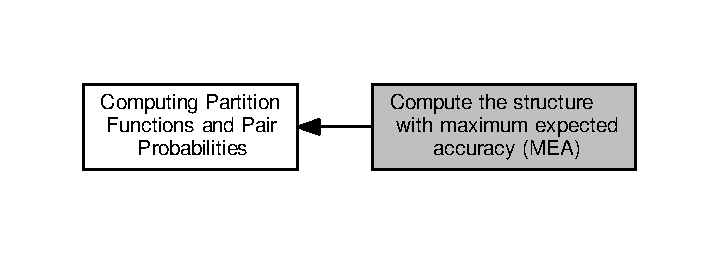
\includegraphics[width=345pt]{group__mea__fold}
\end{center}
\end{figure}

\hypertarget{group__centroid__fold}{}\section{Compute the centroid structure}
\label{group__centroid__fold}\index{Compute the centroid structure@{Compute the centroid structure}}
Collaboration diagram for Compute the centroid structure\+:
\nopagebreak
\begin{figure}[H]
\begin{center}
\leavevmode
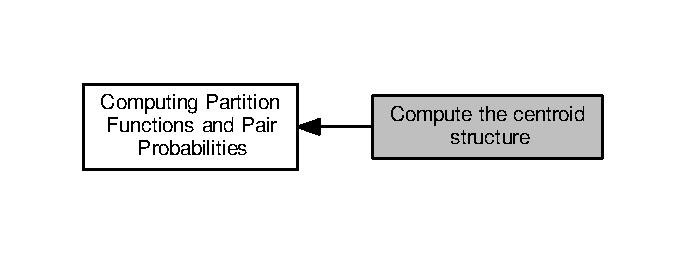
\includegraphics[width=329pt]{group__centroid__fold}
\end{center}
\end{figure}
\subsection*{Functions}
\begin{DoxyCompactItemize}
\item 
char $\ast$ \hyperlink{group__centroid__fold_ga0e64bb67e51963dc71cbd4d30b80a018}{vrna\+\_\+centroid} (\hyperlink{group__fold__compound_ga1b0cef17fd40466cef5968eaeeff6166}{vrna\+\_\+fold\+\_\+compound\+\_\+t} $\ast$vc, double $\ast$dist)
\begin{DoxyCompactList}\small\item\em Get the centroid structure of the ensemble. \end{DoxyCompactList}\item 
char $\ast$ \hyperlink{group__centroid__fold_ga70525a53b879c1427f9ea546c96fa1c5}{vrna\+\_\+centroid\+\_\+from\+\_\+plist} (int length, double $\ast$dist, \hyperlink{group__data__structures_ga8e4eb5e1bfc95776559575beb359af87}{vrna\+\_\+plist\+\_\+t} $\ast$pl)
\begin{DoxyCompactList}\small\item\em Get the centroid structure of the ensemble. \end{DoxyCompactList}\item 
char $\ast$ \hyperlink{group__centroid__fold_ga98193ede06778a9ea966cc8fc43d0804}{vrna\+\_\+centroid\+\_\+from\+\_\+probs} (int length, double $\ast$dist, \hyperlink{group__data__structures_ga31125aeace516926bf7f251f759b6126}{F\+L\+T\+\_\+\+O\+R\+\_\+\+D\+B\+L} $\ast$probs)
\begin{DoxyCompactList}\small\item\em Get the centroid structure of the ensemble. \end{DoxyCompactList}\end{DoxyCompactItemize}


\subsection{Detailed Description}


\subsection{Function Documentation}
\hypertarget{group__centroid__fold_ga0e64bb67e51963dc71cbd4d30b80a018}{}\index{Compute the centroid structure@{Compute the centroid structure}!vrna\+\_\+centroid@{vrna\+\_\+centroid}}
\index{vrna\+\_\+centroid@{vrna\+\_\+centroid}!Compute the centroid structure@{Compute the centroid structure}}
\subsubsection[{vrna\+\_\+centroid}]{\setlength{\rightskip}{0pt plus 5cm}char$\ast$ vrna\+\_\+centroid (
\begin{DoxyParamCaption}
\item[{{\bf vrna\+\_\+fold\+\_\+compound\+\_\+t} $\ast$}]{vc, }
\item[{double $\ast$}]{dist}
\end{DoxyParamCaption}
)}\label{group__centroid__fold_ga0e64bb67e51963dc71cbd4d30b80a018}


{\ttfamily \#include $<$\hyperlink{centroid_8h}{Vienna\+R\+N\+A/centroid.\+h}$>$}



Get the centroid structure of the ensemble. 

The centroid is the structure with the minimal average distance to all other structures ~\newline
 $ <d(S)> = \sum_{(i,j) \in S} (1-p_{ij}) + \sum_{(i,j) \notin S} p_{ij} $ ~\newline
Thus, the centroid is simply the structure containing all pairs with $p_ij>0.5$ The distance of the centroid to the ensemble is written to the memory adressed by {\itshape dist}.


\begin{DoxyParams}[1]{Parameters}
\mbox{\tt in}  & {\em vc} & The fold compound data structure \\
\hline
\mbox{\tt out}  & {\em dist} & A pointer to the distance variable where the centroid distance will be written to \\
\hline
\end{DoxyParams}
\begin{DoxyReturn}{Returns}
The centroid structure of the ensemble in dot-\/bracket notation 
\end{DoxyReturn}
\hypertarget{group__centroid__fold_ga70525a53b879c1427f9ea546c96fa1c5}{}\index{Compute the centroid structure@{Compute the centroid structure}!vrna\+\_\+centroid\+\_\+from\+\_\+plist@{vrna\+\_\+centroid\+\_\+from\+\_\+plist}}
\index{vrna\+\_\+centroid\+\_\+from\+\_\+plist@{vrna\+\_\+centroid\+\_\+from\+\_\+plist}!Compute the centroid structure@{Compute the centroid structure}}
\subsubsection[{vrna\+\_\+centroid\+\_\+from\+\_\+plist}]{\setlength{\rightskip}{0pt plus 5cm}char$\ast$ vrna\+\_\+centroid\+\_\+from\+\_\+plist (
\begin{DoxyParamCaption}
\item[{int}]{length, }
\item[{double $\ast$}]{dist, }
\item[{{\bf vrna\+\_\+plist\+\_\+t} $\ast$}]{pl}
\end{DoxyParamCaption}
)}\label{group__centroid__fold_ga70525a53b879c1427f9ea546c96fa1c5}


{\ttfamily \#include $<$\hyperlink{centroid_8h}{Vienna\+R\+N\+A/centroid.\+h}$>$}



Get the centroid structure of the ensemble. 

This function is a threadsafe replacement for \hyperlink{part__func_8h_ae89a63bd83e75a80b2ba36d20b31ce81}{centroid()} with a \hyperlink{group__data__structures_ga8e4eb5e1bfc95776559575beb359af87}{vrna\+\_\+plist\+\_\+t} input

The centroid is the structure with the minimal average distance to all other structures ~\newline
 $ <d(S)> = \sum_{(i,j) \in S} (1-p_{ij}) + \sum_{(i,j) \notin S} p_{ij} $ ~\newline
Thus, the centroid is simply the structure containing all pairs with $p_ij>0.5$ The distance of the centroid to the ensemble is written to the memory adressed by {\itshape dist}.


\begin{DoxyParams}[1]{Parameters}
\mbox{\tt in}  & {\em length} & The length of the sequence \\
\hline
\mbox{\tt out}  & {\em dist} & A pointer to the distance variable where the centroid distance will be written to \\
\hline
\mbox{\tt in}  & {\em pl} & A pair list containing base pair probability information about the ensemble \\
\hline
\end{DoxyParams}
\begin{DoxyReturn}{Returns}
The centroid structure of the ensemble in dot-\/bracket notation 
\end{DoxyReturn}
\hypertarget{group__centroid__fold_ga98193ede06778a9ea966cc8fc43d0804}{}\index{Compute the centroid structure@{Compute the centroid structure}!vrna\+\_\+centroid\+\_\+from\+\_\+probs@{vrna\+\_\+centroid\+\_\+from\+\_\+probs}}
\index{vrna\+\_\+centroid\+\_\+from\+\_\+probs@{vrna\+\_\+centroid\+\_\+from\+\_\+probs}!Compute the centroid structure@{Compute the centroid structure}}
\subsubsection[{vrna\+\_\+centroid\+\_\+from\+\_\+probs}]{\setlength{\rightskip}{0pt plus 5cm}char$\ast$ vrna\+\_\+centroid\+\_\+from\+\_\+probs (
\begin{DoxyParamCaption}
\item[{int}]{length, }
\item[{double $\ast$}]{dist, }
\item[{{\bf F\+L\+T\+\_\+\+O\+R\+\_\+\+D\+B\+L} $\ast$}]{probs}
\end{DoxyParamCaption}
)}\label{group__centroid__fold_ga98193ede06778a9ea966cc8fc43d0804}


{\ttfamily \#include $<$\hyperlink{centroid_8h}{Vienna\+R\+N\+A/centroid.\+h}$>$}



Get the centroid structure of the ensemble. 

This function is a threadsafe replacement for \hyperlink{part__func_8h_ae89a63bd83e75a80b2ba36d20b31ce81}{centroid()} with a probability array input

The centroid is the structure with the minimal average distance to all other structures ~\newline
 $ <d(S)> = \sum_{(i,j) \in S} (1-p_{ij}) + \sum_{(i,j) \notin S} p_{ij} $ ~\newline
Thus, the centroid is simply the structure containing all pairs with $p_ij>0.5$ The distance of the centroid to the ensemble is written to the memory adressed by {\itshape dist}.


\begin{DoxyParams}[1]{Parameters}
\mbox{\tt in}  & {\em length} & The length of the sequence \\
\hline
\mbox{\tt out}  & {\em dist} & A pointer to the distance variable where the centroid distance will be written to \\
\hline
\mbox{\tt in}  & {\em probs} & An upper triangular matrix containing base pair probabilities (access via iindx \hyperlink{group__utils_ga70b180e9ea764218a82647a1cd347445}{vrna\+\_\+idx\+\_\+row\+\_\+wise()} ) \\
\hline
\end{DoxyParams}
\begin{DoxyReturn}{Returns}
The centroid structure of the ensemble in dot-\/bracket notation 
\end{DoxyReturn}

\hypertarget{group__subopt__fold}{}\section{Enumerating Suboptimal Structures}
\label{group__subopt__fold}\index{Enumerating Suboptimal Structures@{Enumerating Suboptimal Structures}}
Collaboration diagram for Enumerating Suboptimal Structures\+:
\nopagebreak
\begin{figure}[H]
\begin{center}
\leavevmode
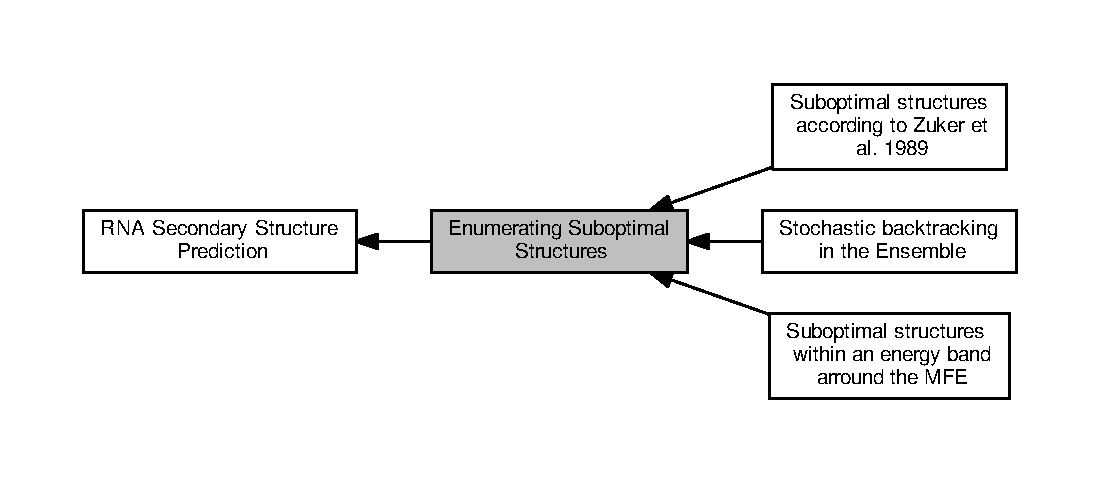
\includegraphics[width=350pt]{group__subopt__fold}
\end{center}
\end{figure}
\subsection*{Modules}
\begin{DoxyCompactItemize}
\item 
\hyperlink{group__subopt__zuker}{Suboptimal structures according to Zuker et al. 1989}
\item 
\hyperlink{group__subopt__wuchty}{Suboptimal structures within an energy band arround the M\+F\+E}
\item 
\hyperlink{group__subopt__stochbt}{Stochastic backtracking in the Ensemble}
\end{DoxyCompactItemize}
\subsection*{Files}
\begin{DoxyCompactItemize}
\item 
file \hyperlink{subopt_8h}{subopt.\+h}
\begin{DoxyCompactList}\small\item\em R\+N\+Asubopt and density of states declarations. \end{DoxyCompactList}\end{DoxyCompactItemize}


\subsection{Detailed Description}

\hypertarget{group__subopt__zuker}{}\section{Suboptimal structures according to Zuker et al. 1989}
\label{group__subopt__zuker}\index{Suboptimal structures according to Zuker et al. 1989@{Suboptimal structures according to Zuker et al. 1989}}
Collaboration diagram for Suboptimal structures according to Zuker et al. 1989\+:
\nopagebreak
\begin{figure}[H]
\begin{center}
\leavevmode
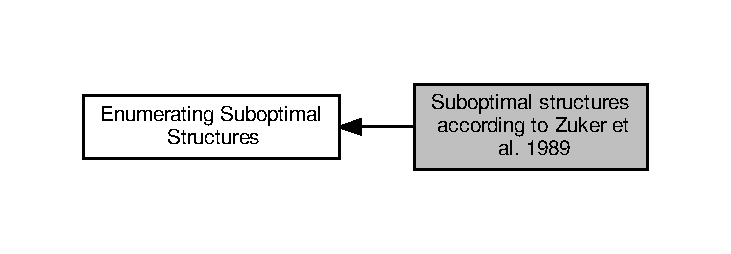
\includegraphics[width=350pt]{group__subopt__zuker}
\end{center}
\end{figure}
\subsection*{Functions}
\begin{DoxyCompactItemize}
\item 
\hyperlink{structvrna__subopt__sol__s}{vrna\+\_\+subopt\+\_\+solution\+\_\+t} $\ast$ \hyperlink{group__subopt__zuker_gac0df98085abd242c7a6b1c868b3a35c8}{vrna\+\_\+subopt\+\_\+zuker} (\hyperlink{group__fold__compound_ga1b0cef17fd40466cef5968eaeeff6166}{vrna\+\_\+fold\+\_\+compound\+\_\+t} $\ast$vc)
\begin{DoxyCompactList}\small\item\em Compute Zuker type suboptimal structures. \end{DoxyCompactList}\item 
\hyperlink{structvrna__subopt__sol__s}{S\+O\+L\+U\+T\+I\+O\+N} $\ast$ \hyperlink{group__subopt__zuker_ga0d5104e3ecf119d8eabd40aa5fe47f90}{zukersubopt} (const char $\ast$string)
\begin{DoxyCompactList}\small\item\em Compute Zuker type suboptimal structures. \end{DoxyCompactList}\item 
\hyperlink{structvrna__subopt__sol__s}{S\+O\+L\+U\+T\+I\+O\+N} $\ast$ \hyperlink{group__subopt__zuker_gab6d0ea8cc1d02f6dd831ca81043c9eb8}{zukersubopt\+\_\+par} (const char $\ast$string, \hyperlink{group__energy__parameters_ga8a69ca7d787e4fd6079914f5343a1f35}{vrna\+\_\+param\+\_\+t} $\ast$parameters)
\begin{DoxyCompactList}\small\item\em Compute Zuker type suboptimal structures. \end{DoxyCompactList}\end{DoxyCompactItemize}


\subsection{Detailed Description}


\subsection{Function Documentation}
\hypertarget{group__subopt__zuker_gac0df98085abd242c7a6b1c868b3a35c8}{}\index{Suboptimal structures according to Zuker et al. 1989@{Suboptimal structures according to Zuker et al. 1989}!vrna\+\_\+subopt\+\_\+zuker@{vrna\+\_\+subopt\+\_\+zuker}}
\index{vrna\+\_\+subopt\+\_\+zuker@{vrna\+\_\+subopt\+\_\+zuker}!Suboptimal structures according to Zuker et al. 1989@{Suboptimal structures according to Zuker et al. 1989}}
\subsubsection[{vrna\+\_\+subopt\+\_\+zuker}]{\setlength{\rightskip}{0pt plus 5cm}{\bf vrna\+\_\+subopt\+\_\+solution\+\_\+t}$\ast$ vrna\+\_\+subopt\+\_\+zuker (
\begin{DoxyParamCaption}
\item[{{\bf vrna\+\_\+fold\+\_\+compound\+\_\+t} $\ast$}]{vc}
\end{DoxyParamCaption}
)}\label{group__subopt__zuker_gac0df98085abd242c7a6b1c868b3a35c8}


{\ttfamily \#include $<$\hyperlink{subopt_8h}{Vienna\+R\+N\+A/subopt.\+h}$>$}



Compute Zuker type suboptimal structures. 

Compute Suboptimal structures according to M. Zuker \cite{zuker:1989} , i.\+e. for every possible base pair the minimum energy structure containing the resp. base pair. Returns a list of these structures and their energies.

\begin{DoxyNote}{Note}
This function internally uses the cofold implementation to compute the suboptimal structures. For that purpose, the function doubles the sequence and enlarges the D\+P matrices, which in fact will grow by a factor of 4 during the computation! At the end of the structure prediction, everything will be re-\/set to its original requriements, i.\+e. normal sequence, normal (empty) D\+P matrices.
\end{DoxyNote}
\begin{DoxyRefDesc}{Bug}
\item[\hyperlink{bug__bug000001}{Bug}]Due to resizing, any pre-\/existing constraints will be lost!\end{DoxyRefDesc}


\begin{DoxySeeAlso}{See also}
\hyperlink{group__subopt__wuchty_ga7988544ae3fc6334c1517cf76e5660aa}{vrna\+\_\+subopt()}, \hyperlink{group__subopt__zuker_ga0d5104e3ecf119d8eabd40aa5fe47f90}{zukersubopt()}, \hyperlink{group__subopt__zuker_gab6d0ea8cc1d02f6dd831ca81043c9eb8}{zukersubopt\+\_\+par()}
\end{DoxySeeAlso}

\begin{DoxyParams}{Parameters}
{\em vc} & fold compound \\
\hline
\end{DoxyParams}
\begin{DoxyReturn}{Returns}
List of zuker suboptimal structures 
\end{DoxyReturn}
\hypertarget{group__subopt__zuker_ga0d5104e3ecf119d8eabd40aa5fe47f90}{}\index{Suboptimal structures according to Zuker et al. 1989@{Suboptimal structures according to Zuker et al. 1989}!zukersubopt@{zukersubopt}}
\index{zukersubopt@{zukersubopt}!Suboptimal structures according to Zuker et al. 1989@{Suboptimal structures according to Zuker et al. 1989}}
\subsubsection[{zukersubopt}]{\setlength{\rightskip}{0pt plus 5cm}{\bf S\+O\+L\+U\+T\+I\+O\+N}$\ast$ zukersubopt (
\begin{DoxyParamCaption}
\item[{const char $\ast$}]{string}
\end{DoxyParamCaption}
)}\label{group__subopt__zuker_ga0d5104e3ecf119d8eabd40aa5fe47f90}


{\ttfamily \#include $<$\hyperlink{subopt_8h}{Vienna\+R\+N\+A/subopt.\+h}$>$}



Compute Zuker type suboptimal structures. 

Compute Suboptimal structures according to M. Zuker, i.\+e. for every possible base pair the minimum energy structure containing the resp. base pair. Returns a list of these structures and their energies.

\begin{DoxyRefDesc}{Deprecated}
\item[\hyperlink{deprecated__deprecated000151}{Deprecated}]use vrna\+\_\+zukersubopt() instead\end{DoxyRefDesc}



\begin{DoxyParams}{Parameters}
{\em string} & R\+N\+A sequence \\
\hline
\end{DoxyParams}
\begin{DoxyReturn}{Returns}
List of zuker suboptimal structures 
\end{DoxyReturn}
\hypertarget{group__subopt__zuker_gab6d0ea8cc1d02f6dd831ca81043c9eb8}{}\index{Suboptimal structures according to Zuker et al. 1989@{Suboptimal structures according to Zuker et al. 1989}!zukersubopt\+\_\+par@{zukersubopt\+\_\+par}}
\index{zukersubopt\+\_\+par@{zukersubopt\+\_\+par}!Suboptimal structures according to Zuker et al. 1989@{Suboptimal structures according to Zuker et al. 1989}}
\subsubsection[{zukersubopt\+\_\+par}]{\setlength{\rightskip}{0pt plus 5cm}{\bf S\+O\+L\+U\+T\+I\+O\+N}$\ast$ zukersubopt\+\_\+par (
\begin{DoxyParamCaption}
\item[{const char $\ast$}]{string, }
\item[{{\bf vrna\+\_\+param\+\_\+t} $\ast$}]{parameters}
\end{DoxyParamCaption}
)}\label{group__subopt__zuker_gab6d0ea8cc1d02f6dd831ca81043c9eb8}


{\ttfamily \#include $<$\hyperlink{subopt_8h}{Vienna\+R\+N\+A/subopt.\+h}$>$}



Compute Zuker type suboptimal structures. 

\begin{DoxyRefDesc}{Deprecated}
\item[\hyperlink{deprecated__deprecated000152}{Deprecated}]use vrna\+\_\+zukersubopt() instead\end{DoxyRefDesc}

\hypertarget{group__subopt__wuchty}{}\section{Suboptimal structures within an energy band arround the M\+F\+E}
\label{group__subopt__wuchty}\index{Suboptimal structures within an energy band arround the M\+F\+E@{Suboptimal structures within an energy band arround the M\+F\+E}}
Collaboration diagram for Suboptimal structures within an energy band arround the M\+F\+E\+:
\nopagebreak
\begin{figure}[H]
\begin{center}
\leavevmode
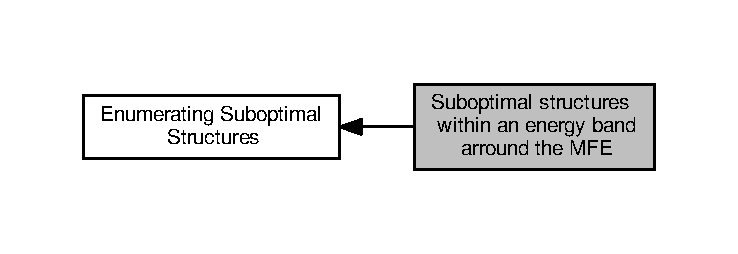
\includegraphics[width=350pt]{group__subopt__wuchty}
\end{center}
\end{figure}
\subsection*{Functions}
\begin{DoxyCompactItemize}
\item 
\hyperlink{structvrna__subopt__sol__s}{vrna\+\_\+subopt\+\_\+solution\+\_\+t} $\ast$ \hyperlink{group__subopt__wuchty_ga7988544ae3fc6334c1517cf76e5660aa}{vrna\+\_\+subopt} (\hyperlink{group__fold__compound_ga1b0cef17fd40466cef5968eaeeff6166}{vrna\+\_\+fold\+\_\+compound\+\_\+t} $\ast$vc, int delta, int sorted, F\+I\+L\+E $\ast$fp)
\begin{DoxyCompactList}\small\item\em Returns list of subopt structures or writes to fp. \end{DoxyCompactList}\item 
\hyperlink{structvrna__subopt__sol__s}{S\+O\+L\+U\+T\+I\+O\+N} $\ast$ \hyperlink{group__subopt__wuchty_ga700f662506a233e42dd7fda74fafd40e}{subopt} (char $\ast$seq, char $\ast$structure, int delta, F\+I\+L\+E $\ast$fp)
\begin{DoxyCompactList}\small\item\em Returns list of subopt structures or writes to fp. \end{DoxyCompactList}\item 
\hypertarget{group__subopt__wuchty_gaa1e1e7031a948ebcb39a9d58d1e9842c}{}\hyperlink{structvrna__subopt__sol__s}{S\+O\+L\+U\+T\+I\+O\+N} $\ast$ \hyperlink{group__subopt__wuchty_gaa1e1e7031a948ebcb39a9d58d1e9842c}{subopt\+\_\+par} (char $\ast$seq, char $\ast$structure, \hyperlink{group__energy__parameters_ga8a69ca7d787e4fd6079914f5343a1f35}{vrna\+\_\+param\+\_\+t} $\ast$parameters, int delta, int is\+\_\+constrained, int is\+\_\+circular, F\+I\+L\+E $\ast$fp)\label{group__subopt__wuchty_gaa1e1e7031a948ebcb39a9d58d1e9842c}

\begin{DoxyCompactList}\small\item\em Returns list of subopt structures or writes to fp. \end{DoxyCompactList}\item 
\hyperlink{structvrna__subopt__sol__s}{S\+O\+L\+U\+T\+I\+O\+N} $\ast$ \hyperlink{group__subopt__wuchty_ga8634516e4740e0b6c9a46d2bae940340}{subopt\+\_\+circ} (char $\ast$seq, char $\ast$sequence, int delta, F\+I\+L\+E $\ast$fp)
\begin{DoxyCompactList}\small\item\em Returns list of circular subopt structures or writes to fp. \end{DoxyCompactList}\end{DoxyCompactItemize}
\subsection*{Variables}
\begin{DoxyCompactItemize}
\item 
\hypertarget{group__subopt__wuchty_ga5e57d914bcb5feeecdf520e25313fcfe}{}double \hyperlink{group__subopt__wuchty_ga5e57d914bcb5feeecdf520e25313fcfe}{print\+\_\+energy}\label{group__subopt__wuchty_ga5e57d914bcb5feeecdf520e25313fcfe}

\begin{DoxyCompactList}\small\item\em printing threshold for use with log\+M\+L \end{DoxyCompactList}\item 
\hypertarget{group__subopt__wuchty_ga873cf8ed69e0437f8efa8b1fec854a0e}{}int \hyperlink{group__subopt__wuchty_ga873cf8ed69e0437f8efa8b1fec854a0e}{subopt\+\_\+sorted}\label{group__subopt__wuchty_ga873cf8ed69e0437f8efa8b1fec854a0e}

\begin{DoxyCompactList}\small\item\em Sort output by energy. \end{DoxyCompactList}\end{DoxyCompactItemize}


\subsection{Detailed Description}


\subsection{Function Documentation}
\hypertarget{group__subopt__wuchty_ga7988544ae3fc6334c1517cf76e5660aa}{}\index{Suboptimal structures within an energy band arround the M\+F\+E@{Suboptimal structures within an energy band arround the M\+F\+E}!vrna\+\_\+subopt@{vrna\+\_\+subopt}}
\index{vrna\+\_\+subopt@{vrna\+\_\+subopt}!Suboptimal structures within an energy band arround the M\+F\+E@{Suboptimal structures within an energy band arround the M\+F\+E}}
\subsubsection[{vrna\+\_\+subopt}]{\setlength{\rightskip}{0pt plus 5cm}{\bf vrna\+\_\+subopt\+\_\+solution\+\_\+t}$\ast$ vrna\+\_\+subopt (
\begin{DoxyParamCaption}
\item[{{\bf vrna\+\_\+fold\+\_\+compound\+\_\+t} $\ast$}]{vc, }
\item[{int}]{delta, }
\item[{int}]{sorted, }
\item[{F\+I\+L\+E $\ast$}]{fp}
\end{DoxyParamCaption}
)}\label{group__subopt__wuchty_ga7988544ae3fc6334c1517cf76e5660aa}


{\ttfamily \#include $<$\hyperlink{subopt_8h}{Vienna\+R\+N\+A/subopt.\+h}$>$}



Returns list of subopt structures or writes to fp. 

This function produces {\bfseries all} suboptimal secondary structures within \textquotesingle{}delta\textquotesingle{} $\ast$ 0.\+01 kcal/mol of the optimum, see \cite{wuchty:1999}. The results are either directly written to a \textquotesingle{}fp\textquotesingle{} (if \textquotesingle{}fp\textquotesingle{} is not N\+U\+L\+L), or (fp==N\+U\+L\+L) returned in a \#vrna\+\_\+subopt\+\_\+solution\+\_\+t $\ast$ list terminated by an entry were the \textquotesingle{}structure\textquotesingle{} member is N\+U\+L\+L.

\begin{DoxySeeAlso}{See also}
\hyperlink{group__subopt__zuker_gac0df98085abd242c7a6b1c868b3a35c8}{vrna\+\_\+subopt\+\_\+zuker()} 
\end{DoxySeeAlso}

\begin{DoxyParams}{Parameters}
{\em vc} & \\
\hline
{\em delta} & \\
\hline
{\em sorted} & Sort results by energy in ascending order \\
\hline
{\em fp} & \\
\hline
\end{DoxyParams}
\begin{DoxyReturn}{Returns}

\end{DoxyReturn}
\hypertarget{group__subopt__wuchty_ga700f662506a233e42dd7fda74fafd40e}{}\index{Suboptimal structures within an energy band arround the M\+F\+E@{Suboptimal structures within an energy band arround the M\+F\+E}!subopt@{subopt}}
\index{subopt@{subopt}!Suboptimal structures within an energy band arround the M\+F\+E@{Suboptimal structures within an energy band arround the M\+F\+E}}
\subsubsection[{subopt}]{\setlength{\rightskip}{0pt plus 5cm}{\bf S\+O\+L\+U\+T\+I\+O\+N}$\ast$ subopt (
\begin{DoxyParamCaption}
\item[{char $\ast$}]{seq, }
\item[{char $\ast$}]{structure, }
\item[{int}]{delta, }
\item[{F\+I\+L\+E $\ast$}]{fp}
\end{DoxyParamCaption}
)}\label{group__subopt__wuchty_ga700f662506a233e42dd7fda74fafd40e}


{\ttfamily \#include $<$\hyperlink{subopt_8h}{Vienna\+R\+N\+A/subopt.\+h}$>$}



Returns list of subopt structures or writes to fp. 

This function produces {\bfseries all} suboptimal secondary structures within \textquotesingle{}delta\textquotesingle{} $\ast$ 0.\+01 kcal/mol of the optimum. The results are either directly written to a \textquotesingle{}fp\textquotesingle{} (if \textquotesingle{}fp\textquotesingle{} is not N\+U\+L\+L), or (fp==N\+U\+L\+L) returned in a \#\+S\+O\+L\+U\+T\+I\+O\+N $\ast$ list terminated by an entry were the \textquotesingle{}structure\textquotesingle{} pointer is N\+U\+L\+L.


\begin{DoxyParams}{Parameters}
{\em seq} & \\
\hline
{\em structure} & \\
\hline
{\em delta} & \\
\hline
{\em fp} & \\
\hline
\end{DoxyParams}
\begin{DoxyReturn}{Returns}

\end{DoxyReturn}
\hypertarget{group__subopt__wuchty_ga8634516e4740e0b6c9a46d2bae940340}{}\index{Suboptimal structures within an energy band arround the M\+F\+E@{Suboptimal structures within an energy band arround the M\+F\+E}!subopt\+\_\+circ@{subopt\+\_\+circ}}
\index{subopt\+\_\+circ@{subopt\+\_\+circ}!Suboptimal structures within an energy band arround the M\+F\+E@{Suboptimal structures within an energy band arround the M\+F\+E}}
\subsubsection[{subopt\+\_\+circ}]{\setlength{\rightskip}{0pt plus 5cm}{\bf S\+O\+L\+U\+T\+I\+O\+N}$\ast$ subopt\+\_\+circ (
\begin{DoxyParamCaption}
\item[{char $\ast$}]{seq, }
\item[{char $\ast$}]{sequence, }
\item[{int}]{delta, }
\item[{F\+I\+L\+E $\ast$}]{fp}
\end{DoxyParamCaption}
)}\label{group__subopt__wuchty_ga8634516e4740e0b6c9a46d2bae940340}


{\ttfamily \#include $<$\hyperlink{subopt_8h}{Vienna\+R\+N\+A/subopt.\+h}$>$}



Returns list of circular subopt structures or writes to fp. 

This function is similar to \hyperlink{group__subopt__wuchty_ga700f662506a233e42dd7fda74fafd40e}{subopt()} but calculates secondary structures assuming the R\+N\+A sequence to be circular instead of linear


\begin{DoxyParams}{Parameters}
{\em seq} & \\
\hline
{\em sequence} & \\
\hline
{\em delta} & \\
\hline
{\em fp} & \\
\hline
\end{DoxyParams}
\begin{DoxyReturn}{Returns}

\end{DoxyReturn}

\hypertarget{group__subopt__stochbt}{}\section{Stochastic backtracking in the Ensemble}
\label{group__subopt__stochbt}\index{Stochastic backtracking in the Ensemble@{Stochastic backtracking in the Ensemble}}
Collaboration diagram for Stochastic backtracking in the Ensemble\+:
\nopagebreak
\begin{figure}[H]
\begin{center}
\leavevmode
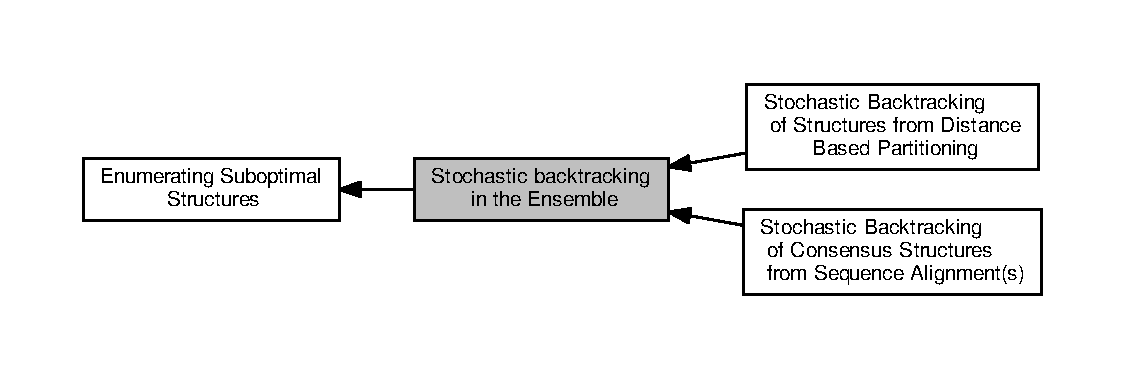
\includegraphics[width=350pt]{group__subopt__stochbt}
\end{center}
\end{figure}
\subsection*{Modules}
\begin{DoxyCompactItemize}
\item 
\hyperlink{group__consensus__stochbt}{Stochastic Backtracking of Consensus Structures from Sequence Alignment(s)}
\item 
\hyperlink{group__kl__neighborhood__stochbt}{Stochastic Backtracking of Structures from Distance Based Partitioning}
\begin{DoxyCompactList}\small\item\em Contains functions related to stochastic backtracking from a specified distance class. \end{DoxyCompactList}\end{DoxyCompactItemize}
\subsection*{Functions}
\begin{DoxyCompactItemize}
\item 
char $\ast$ \hyperlink{group__subopt__stochbt_ga5a3e11d3ce121b5b045cb57f86a8ed05}{vrna\+\_\+pbacktrack5} (\hyperlink{group__fold__compound_ga1b0cef17fd40466cef5968eaeeff6166}{vrna\+\_\+fold\+\_\+compound\+\_\+t} $\ast$vc, int length)
\begin{DoxyCompactList}\small\item\em Sample a secondary structure of a subsequence from the Boltzmann ensemble according its probability. \end{DoxyCompactList}\item 
char $\ast$ \hyperlink{group__subopt__stochbt_ga0429de82e75af6c6e7508f4d273a192f}{vrna\+\_\+pbacktrack} (\hyperlink{group__fold__compound_ga1b0cef17fd40466cef5968eaeeff6166}{vrna\+\_\+fold\+\_\+compound\+\_\+t} $\ast$vc)
\begin{DoxyCompactList}\small\item\em Sample a secondary structure (consensus structure) from the Boltzmann ensemble according its probability. \end{DoxyCompactList}\item 
char $\ast$ \hyperlink{group__subopt__stochbt_gac03ca6db186bb3bf0a2a326d7fb3ba03}{pbacktrack} (char $\ast$sequence)
\begin{DoxyCompactList}\small\item\em Sample a secondary structure from the Boltzmann ensemble according its probability. \end{DoxyCompactList}\item 
char $\ast$ \hyperlink{group__subopt__stochbt_ga00474051204ac9ad576b3e45174d03ff}{pbacktrack\+\_\+circ} (char $\ast$sequence)
\begin{DoxyCompactList}\small\item\em Sample a secondary structure of a circular R\+N\+A from the Boltzmann ensemble according its probability. \end{DoxyCompactList}\end{DoxyCompactItemize}
\subsection*{Variables}
\begin{DoxyCompactItemize}
\item 
int \hyperlink{group__subopt__stochbt_gacd79b1a570e6ad9be24cb11fe8cae30a}{st\+\_\+back}
\begin{DoxyCompactList}\small\item\em Flag indicating that auxilary arrays are needed throughout the computations. This is essential for stochastic backtracking. \end{DoxyCompactList}\end{DoxyCompactItemize}


\subsection{Detailed Description}


\subsection{Function Documentation}
\hypertarget{group__subopt__stochbt_ga5a3e11d3ce121b5b045cb57f86a8ed05}{}\index{Stochastic backtracking in the Ensemble@{Stochastic backtracking in the Ensemble}!vrna\+\_\+pbacktrack5@{vrna\+\_\+pbacktrack5}}
\index{vrna\+\_\+pbacktrack5@{vrna\+\_\+pbacktrack5}!Stochastic backtracking in the Ensemble@{Stochastic backtracking in the Ensemble}}
\subsubsection[{vrna\+\_\+pbacktrack5}]{\setlength{\rightskip}{0pt plus 5cm}char$\ast$ vrna\+\_\+pbacktrack5 (
\begin{DoxyParamCaption}
\item[{{\bf vrna\+\_\+fold\+\_\+compound\+\_\+t} $\ast$}]{vc, }
\item[{int}]{length}
\end{DoxyParamCaption}
)}\label{group__subopt__stochbt_ga5a3e11d3ce121b5b045cb57f86a8ed05}


{\ttfamily \#include $<$\hyperlink{boltzmann__sampling_8h}{Vienna\+R\+N\+A/boltzmann\+\_\+sampling.\+h}$>$}



Sample a secondary structure of a subsequence from the Boltzmann ensemble according its probability. 

\begin{DoxyPrecond}{Precondition}
The fold compound has to be obtained using the \#\+V\+R\+N\+A\+\_\+\+O\+P\+T\+I\+O\+N\+\_\+\+H\+Y\+B\+R\+I\+D option in \hyperlink{group__fold__compound_ga6601d994ba32b11511b36f68b08403be}{vrna\+\_\+fold\+\_\+compound()} 

\hyperlink{group__pf__fold_ga29e256d688ad221b78d37f427e0e99bc}{vrna\+\_\+pf()} has to be called first to fill the partition function matrices
\end{DoxyPrecond}

\begin{DoxyParams}{Parameters}
{\em vc} & The fold compound data structure \\
\hline
{\em length} & The length of the subsequence to consider (starting with 5\textquotesingle{} end) \\
\hline
\end{DoxyParams}
\begin{DoxyReturn}{Returns}
A sampled secondary structure in dot-\/bracket notation 
\end{DoxyReturn}
\hypertarget{group__subopt__stochbt_ga0429de82e75af6c6e7508f4d273a192f}{}\index{Stochastic backtracking in the Ensemble@{Stochastic backtracking in the Ensemble}!vrna\+\_\+pbacktrack@{vrna\+\_\+pbacktrack}}
\index{vrna\+\_\+pbacktrack@{vrna\+\_\+pbacktrack}!Stochastic backtracking in the Ensemble@{Stochastic backtracking in the Ensemble}}
\subsubsection[{vrna\+\_\+pbacktrack}]{\setlength{\rightskip}{0pt plus 5cm}char$\ast$ vrna\+\_\+pbacktrack (
\begin{DoxyParamCaption}
\item[{{\bf vrna\+\_\+fold\+\_\+compound\+\_\+t} $\ast$}]{vc}
\end{DoxyParamCaption}
)}\label{group__subopt__stochbt_ga0429de82e75af6c6e7508f4d273a192f}


{\ttfamily \#include $<$\hyperlink{boltzmann__sampling_8h}{Vienna\+R\+N\+A/boltzmann\+\_\+sampling.\+h}$>$}



Sample a secondary structure (consensus structure) from the Boltzmann ensemble according its probability. 

\begin{DoxyPrecond}{Precondition}
The dynamic programming (D\+P) matrices have to allow for unique multibranch loop decomposition, i.\+e. the \hyperlink{group__model__details_ade065b814a4e2e72ead93ab502613ed2}{vrna\+\_\+md\+\_\+t.\+uniq\+\_\+\+M\+L} flag has to be non-\/zero before calling \hyperlink{group__fold__compound_ga6601d994ba32b11511b36f68b08403be}{vrna\+\_\+fold\+\_\+compound()} 

\hyperlink{group__pf__fold_ga29e256d688ad221b78d37f427e0e99bc}{vrna\+\_\+pf()} has to be called first to fill the partition function matrices
\end{DoxyPrecond}
\begin{DoxyNote}{Note}
This function is polymorphic. It accepts \hyperlink{group__fold__compound_ga1b0cef17fd40466cef5968eaeeff6166}{vrna\+\_\+fold\+\_\+compound\+\_\+t} of type \hyperlink{group__fold__compound_gga01a4ff86fa71deaaa5d1abbd95a1447da1608d3aa78905fc39e0d25a624ac9512}{V\+R\+N\+A\+\_\+\+V\+C\+\_\+\+T\+Y\+P\+E\+\_\+\+S\+I\+N\+G\+L\+E}, and \hyperlink{group__fold__compound_gga01a4ff86fa71deaaa5d1abbd95a1447da056345f1bcfe7cd595d1fd437c05246d}{V\+R\+N\+A\+\_\+\+V\+C\+\_\+\+T\+Y\+P\+E\+\_\+\+A\+L\+I\+G\+N\+M\+E\+N\+T}.

The function will automagically detect cicular R\+N\+As based on the model\+\_\+details in exp\+\_\+params as provided via the \hyperlink{group__fold__compound_ga1b0cef17fd40466cef5968eaeeff6166}{vrna\+\_\+fold\+\_\+compound\+\_\+t}
\end{DoxyNote}

\begin{DoxyParams}{Parameters}
{\em vc} & The fold compound data structure \\
\hline
{\em length} & The length of the subsequence to consider (starting with 5\textquotesingle{} end) \\
\hline
\end{DoxyParams}
\begin{DoxyReturn}{Returns}
A sampled secondary structure in dot-\/bracket notation 
\end{DoxyReturn}
\hypertarget{group__subopt__stochbt_gac03ca6db186bb3bf0a2a326d7fb3ba03}{}\index{Stochastic backtracking in the Ensemble@{Stochastic backtracking in the Ensemble}!pbacktrack@{pbacktrack}}
\index{pbacktrack@{pbacktrack}!Stochastic backtracking in the Ensemble@{Stochastic backtracking in the Ensemble}}
\subsubsection[{pbacktrack}]{\setlength{\rightskip}{0pt plus 5cm}char$\ast$ pbacktrack (
\begin{DoxyParamCaption}
\item[{char $\ast$}]{sequence}
\end{DoxyParamCaption}
)}\label{group__subopt__stochbt_gac03ca6db186bb3bf0a2a326d7fb3ba03}


{\ttfamily \#include $<$\hyperlink{part__func_8h}{Vienna\+R\+N\+A/part\+\_\+func.\+h}$>$}



Sample a secondary structure from the Boltzmann ensemble according its probability. 

\begin{DoxyPrecond}{Precondition}
\hyperlink{group__subopt__stochbt_gacd79b1a570e6ad9be24cb11fe8cae30a}{st\+\_\+back} has to be set to 1 before calling \hyperlink{group__pf__fold_gadc3db3d98742427e7001a7fd36ef28c2}{pf\+\_\+fold()} or \hyperlink{group__pf__fold_gac4f95bee734b2563a3d6e9932117ebdf}{pf\+\_\+fold\+\_\+par()} 

\hyperlink{group__pf__fold_gac4f95bee734b2563a3d6e9932117ebdf}{pf\+\_\+fold\+\_\+par()} or \hyperlink{group__pf__fold_gadc3db3d98742427e7001a7fd36ef28c2}{pf\+\_\+fold()} have to be called first to fill the partition function matrices
\end{DoxyPrecond}

\begin{DoxyParams}{Parameters}
{\em sequence} & The R\+N\+A sequence \\
\hline
\end{DoxyParams}
\begin{DoxyReturn}{Returns}
A sampled secondary structure in dot-\/bracket notation 
\end{DoxyReturn}
\hypertarget{group__subopt__stochbt_ga00474051204ac9ad576b3e45174d03ff}{}\index{Stochastic backtracking in the Ensemble@{Stochastic backtracking in the Ensemble}!pbacktrack\+\_\+circ@{pbacktrack\+\_\+circ}}
\index{pbacktrack\+\_\+circ@{pbacktrack\+\_\+circ}!Stochastic backtracking in the Ensemble@{Stochastic backtracking in the Ensemble}}
\subsubsection[{pbacktrack\+\_\+circ}]{\setlength{\rightskip}{0pt plus 5cm}char$\ast$ pbacktrack\+\_\+circ (
\begin{DoxyParamCaption}
\item[{char $\ast$}]{sequence}
\end{DoxyParamCaption}
)}\label{group__subopt__stochbt_ga00474051204ac9ad576b3e45174d03ff}


{\ttfamily \#include $<$\hyperlink{part__func_8h}{Vienna\+R\+N\+A/part\+\_\+func.\+h}$>$}



Sample a secondary structure of a circular R\+N\+A from the Boltzmann ensemble according its probability. 

This function does the same as \hyperlink{group__subopt__stochbt_gac03ca6db186bb3bf0a2a326d7fb3ba03}{pbacktrack()} but assumes the R\+N\+A molecule to be circular

\begin{DoxyPrecond}{Precondition}
\hyperlink{group__subopt__stochbt_gacd79b1a570e6ad9be24cb11fe8cae30a}{st\+\_\+back} has to be set to 1 before calling \hyperlink{group__pf__fold_gadc3db3d98742427e7001a7fd36ef28c2}{pf\+\_\+fold()} or \hyperlink{group__pf__fold_gac4f95bee734b2563a3d6e9932117ebdf}{pf\+\_\+fold\+\_\+par()} 

\hyperlink{group__pf__fold_gac4f95bee734b2563a3d6e9932117ebdf}{pf\+\_\+fold\+\_\+par()} or \hyperlink{group__pf__fold_ga819ce5fca8984004ac81c4a3b04cb735}{pf\+\_\+circ\+\_\+fold()} have to be called first to fill the partition function matrices
\end{DoxyPrecond}
\begin{DoxyRefDesc}{Deprecated}
\item[\hyperlink{deprecated__deprecated000103}{Deprecated}]Use \hyperlink{group__subopt__stochbt_ga0429de82e75af6c6e7508f4d273a192f}{vrna\+\_\+pbacktrack()} instead.\end{DoxyRefDesc}



\begin{DoxyParams}{Parameters}
{\em sequence} & The R\+N\+A sequence \\
\hline
\end{DoxyParams}
\begin{DoxyReturn}{Returns}
A sampled secondary structure in dot-\/bracket notation 
\end{DoxyReturn}


\subsection{Variable Documentation}
\hypertarget{group__subopt__stochbt_gacd79b1a570e6ad9be24cb11fe8cae30a}{}\index{Stochastic backtracking in the Ensemble@{Stochastic backtracking in the Ensemble}!st\+\_\+back@{st\+\_\+back}}
\index{st\+\_\+back@{st\+\_\+back}!Stochastic backtracking in the Ensemble@{Stochastic backtracking in the Ensemble}}
\subsubsection[{st\+\_\+back}]{\setlength{\rightskip}{0pt plus 5cm}int st\+\_\+back}\label{group__subopt__stochbt_gacd79b1a570e6ad9be24cb11fe8cae30a}


{\ttfamily \#include $<$\hyperlink{part__func_8h}{Vienna\+R\+N\+A/part\+\_\+func.\+h}$>$}



Flag indicating that auxilary arrays are needed throughout the computations. This is essential for stochastic backtracking. 

Set this variable to 1 prior to a call of \hyperlink{group__pf__fold_gadc3db3d98742427e7001a7fd36ef28c2}{pf\+\_\+fold()} to ensure that all matrices needed for stochastic backtracking are filled in the forward recursions

\begin{DoxyRefDesc}{Deprecated}
\item[\hyperlink{deprecated__deprecated000100}{Deprecated}]set the {\itshape uniq\+\_\+\+M\+L} flag in \hyperlink{group__model__details_ga1f8a10e12a0a1915f2a4eff0b28ea17c}{vrna\+\_\+md\+\_\+t} before passing it to \hyperlink{group__fold__compound_ga6601d994ba32b11511b36f68b08403be}{vrna\+\_\+fold\+\_\+compound()}.\end{DoxyRefDesc}


\begin{DoxySeeAlso}{See also}
\hyperlink{group__subopt__stochbt_gac03ca6db186bb3bf0a2a326d7fb3ba03}{pbacktrack()}, \hyperlink{group__subopt__stochbt_ga00474051204ac9ad576b3e45174d03ff}{pbacktrack\+\_\+circ} 
\end{DoxySeeAlso}

\hypertarget{group__cofold}{}\section{Calculate Secondary Structures of two R\+N\+As upon Dimerization}
\label{group__cofold}\index{Calculate Secondary Structures of two R\+N\+As upon Dimerization@{Calculate Secondary Structures of two R\+N\+As upon Dimerization}}


Predict structures formed by two molecules upon hybridization.  


Collaboration diagram for Calculate Secondary Structures of two R\+N\+As upon Dimerization\+:
\nopagebreak
\begin{figure}[H]
\begin{center}
\leavevmode
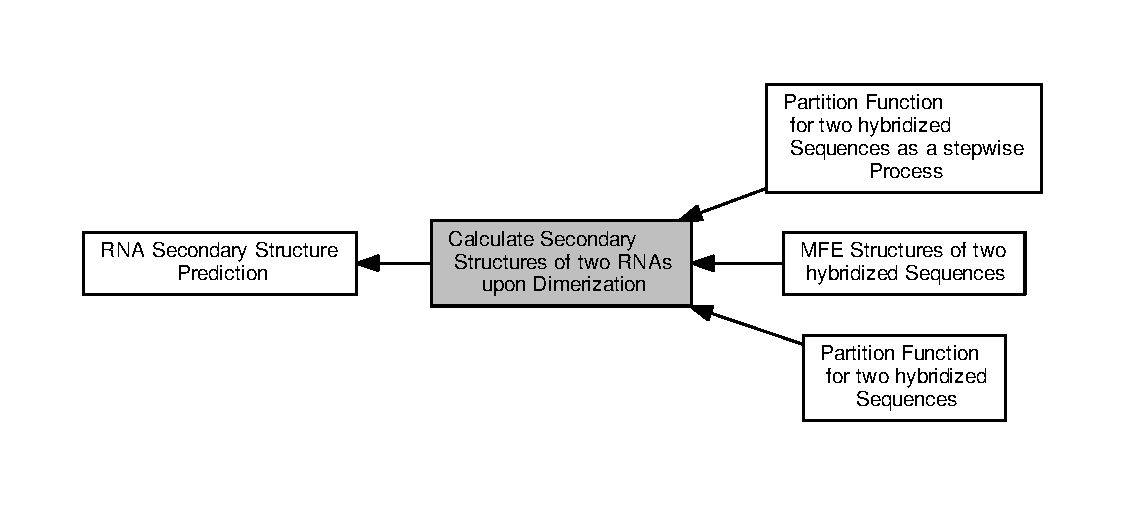
\includegraphics[width=350pt]{group__cofold}
\end{center}
\end{figure}
\subsection*{Modules}
\begin{DoxyCompactItemize}
\item 
\hyperlink{group__mfe__cofold}{M\+F\+E Structures of two hybridized Sequences}
\item 
\hyperlink{group__pf__cofold}{Partition Function for two hybridized Sequences}
\begin{DoxyCompactList}\small\item\em Partition Function Cofolding. \end{DoxyCompactList}\item 
\hyperlink{group__up__cofold}{Partition Function for two hybridized Sequences as a stepwise Process}
\begin{DoxyCompactList}\small\item\em Partition Function Cofolding as a stepwise process. \end{DoxyCompactList}\end{DoxyCompactItemize}


\subsection{Detailed Description}
Predict structures formed by two molecules upon hybridization. 

The function of an R\+N\+A molecule often depends on its interaction with other R\+N\+As. The following routines therefore allow to predict structures formed by two R\+N\+A molecules upon hybridization.~\newline
One approach to co-\/folding two R\+N\+As consists of concatenating the two sequences and keeping track of the concatenation point in all energy evaluations. Correspondingly, many of the \hyperlink{group__mfe__cofold_gabc8517f22cfe70595ee81fc837910d52}{cofold()} and \hyperlink{part__func__co_8h_ae5c1e7331718669bdae7a86de2be6184}{co\+\_\+pf\+\_\+fold()} routines below take one sequence string as argument and use the the global variable \hyperlink{fold__vars_8h_ab9b2c3a37a5516614c06d0ab54b97cda}{cut\+\_\+point} to mark the concatenation point. Note that while the {\itshape R\+N\+Acofold} program uses the \textquotesingle{}\&\textquotesingle{} character to mark the chain break in its input, you should not use an \textquotesingle{}\&\textquotesingle{} when using the library routines (set \hyperlink{fold__vars_8h_ab9b2c3a37a5516614c06d0ab54b97cda}{cut\+\_\+point} instead).~\newline
In a second approach to co-\/folding two R\+N\+As, cofolding is seen as a stepwise process. In the first step the probability of an unpaired region is calculated and in a second step this probability of an unpaired region is multiplied with the probability of an interaction between the two R\+N\+As. This approach is implemented for the interaction between a long target sequence and a short ligand R\+N\+A. Function \hyperlink{group__up__cofold_ga5b4ee40e190d2f633cd01cf0d2fe93cf}{pf\+\_\+unstru()} calculates the partition function over all unpaired regions in the input sequence. Function \hyperlink{group__up__cofold_ga1aa0aa02bc3a724f87360c03097afd00}{pf\+\_\+interact()}, which calculates the partition function over all possible interactions between two sequences, needs both sequence as separate strings as input. 
\hypertarget{group__mfe__fold__single}{}\section{M\+F\+E Structures of single Nucleic Acid Sequences}
\label{group__mfe__fold__single}\index{M\+F\+E Structures of single Nucleic Acid Sequences@{M\+F\+E Structures of single Nucleic Acid Sequences}}


This module contains all functions and variables related to the calculation of global minimum free energy structures for single sequences.  


Collaboration diagram for M\+F\+E Structures of single Nucleic Acid Sequences\+:
\nopagebreak
\begin{figure}[H]
\begin{center}
\leavevmode
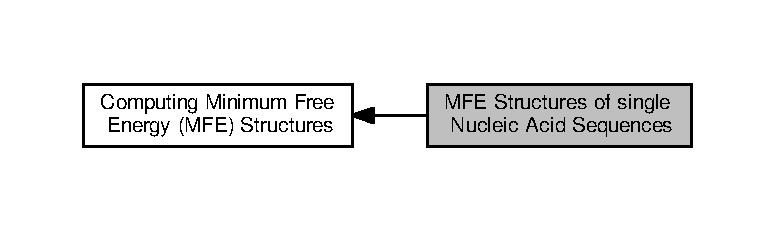
\includegraphics[width=350pt]{group__mfe__fold__single}
\end{center}
\end{figure}
\subsection*{Functions}
\begin{DoxyCompactItemize}
\item 
float \hyperlink{group__mfe__fold__single_gae7ca49ffb3086f145da36c964a7cec64}{vrna\+\_\+fold} (const char $\ast$string, char $\ast$structure)
\begin{DoxyCompactList}\small\item\em Compute Minimum Free Energy (M\+F\+E), and a corresponding secondary structure for an R\+N\+A sequence. \end{DoxyCompactList}\item 
float \hyperlink{group__mfe__fold__single_gaa0f5bf321038f404b36a6147bdae4154}{vrna\+\_\+circfold} (const char $\ast$string, char $\ast$structure)
\begin{DoxyCompactList}\small\item\em Compute Minimum Free Energy (M\+F\+E), and a corresponding secondary structure for a circular R\+N\+A sequence. \end{DoxyCompactList}\item 
float \hyperlink{group__mfe__fold__single_ga2bc41df5d71fee6fd8da9904ee65d8fb}{fold\+\_\+par} (const char $\ast$sequence, char $\ast$structure, \hyperlink{group__energy__parameters_ga8a69ca7d787e4fd6079914f5343a1f35}{vrna\+\_\+param\+\_\+t} $\ast$parameters, int is\+\_\+constrained, int is\+\_\+circular)
\begin{DoxyCompactList}\small\item\em Compute minimum free energy and an appropriate secondary structure of an R\+N\+A sequence. \end{DoxyCompactList}\item 
float \hyperlink{group__mfe__fold__single_gaadafcb0f140795ae62e5ca027e335a9b}{fold} (const char $\ast$sequence, char $\ast$structure)
\begin{DoxyCompactList}\small\item\em Compute minimum free energy and an appropriate secondary structure of an R\+N\+A sequence. \end{DoxyCompactList}\item 
float \hyperlink{group__mfe__fold__single_ga4ac63ab3e8d9a80ced28b8052d94e423}{circfold} (const char $\ast$sequence, char $\ast$structure)
\begin{DoxyCompactList}\small\item\em Compute minimum free energy and an appropriate secondary structure of a circular R\+N\+A sequence. \end{DoxyCompactList}\item 
void \hyperlink{group__mfe__fold__single_ga107fdfe5fd641868156bfd849f6866c7}{free\+\_\+arrays} (void)
\begin{DoxyCompactList}\small\item\em Free arrays for mfe folding. \end{DoxyCompactList}\item 
void \hyperlink{group__mfe__fold__single_ga41bf8f6fa15b94471f7095cad9f0ccf3}{update\+\_\+fold\+\_\+params} (void)
\begin{DoxyCompactList}\small\item\em Recalculate energy parameters. \end{DoxyCompactList}\item 
void \hyperlink{group__mfe__fold__single_gae66dc422efb8f5d56717d92d6002a9f8}{update\+\_\+fold\+\_\+params\+\_\+par} (\hyperlink{group__energy__parameters_ga8a69ca7d787e4fd6079914f5343a1f35}{vrna\+\_\+param\+\_\+t} $\ast$parameters)
\begin{DoxyCompactList}\small\item\em Recalculate energy parameters. \end{DoxyCompactList}\item 
void \hyperlink{group__mfe__fold__single_ga99641b8dbb40891da5490d3cc271e607}{export\+\_\+fold\+\_\+arrays} (int $\ast$$\ast$f5\+\_\+p, int $\ast$$\ast$c\+\_\+p, int $\ast$$\ast$f\+M\+L\+\_\+p, int $\ast$$\ast$f\+M1\+\_\+p, int $\ast$$\ast$indx\+\_\+p, char $\ast$$\ast$ptype\+\_\+p)
\item 
void \hyperlink{group__mfe__fold__single_ga6606ec0ec964ea506fdadb997a1a5328}{export\+\_\+fold\+\_\+arrays\+\_\+par} (int $\ast$$\ast$f5\+\_\+p, int $\ast$$\ast$c\+\_\+p, int $\ast$$\ast$f\+M\+L\+\_\+p, int $\ast$$\ast$f\+M1\+\_\+p, int $\ast$$\ast$indx\+\_\+p, char $\ast$$\ast$ptype\+\_\+p, \hyperlink{group__energy__parameters_ga8a69ca7d787e4fd6079914f5343a1f35}{vrna\+\_\+param\+\_\+t} $\ast$$\ast$P\+\_\+p)
\item 
void \hyperlink{group__mfe__fold__single_ga04d5d639fd4473ca766436a9bae5665c}{export\+\_\+circfold\+\_\+arrays} (int $\ast$Fc\+\_\+p, int $\ast$Fc\+H\+\_\+p, int $\ast$Fc\+I\+\_\+p, int $\ast$Fc\+M\+\_\+p, int $\ast$$\ast$f\+M2\+\_\+p, int $\ast$$\ast$f5\+\_\+p, int $\ast$$\ast$c\+\_\+p, int $\ast$$\ast$f\+M\+L\+\_\+p, int $\ast$$\ast$f\+M1\+\_\+p, int $\ast$$\ast$indx\+\_\+p, char $\ast$$\ast$ptype\+\_\+p)
\item 
void \hyperlink{group__mfe__fold__single_ga004bb901e7fd2f8d5ae68f9530318ce1}{export\+\_\+circfold\+\_\+arrays\+\_\+par} (int $\ast$Fc\+\_\+p, int $\ast$Fc\+H\+\_\+p, int $\ast$Fc\+I\+\_\+p, int $\ast$Fc\+M\+\_\+p, int $\ast$$\ast$f\+M2\+\_\+p, int $\ast$$\ast$f5\+\_\+p, int $\ast$$\ast$c\+\_\+p, int $\ast$$\ast$f\+M\+L\+\_\+p, int $\ast$$\ast$f\+M1\+\_\+p, int $\ast$$\ast$indx\+\_\+p, char $\ast$$\ast$ptype\+\_\+p, \hyperlink{group__energy__parameters_ga8a69ca7d787e4fd6079914f5343a1f35}{vrna\+\_\+param\+\_\+t} $\ast$$\ast$P\+\_\+p)
\item 
int \hyperlink{group__mfe__fold__single_ga2163034a25c6115d894b199e97e03f6c}{Loop\+Energy} (int n1, int n2, int type, int type\+\_\+2, int si1, int sj1, int sp1, int sq1)
\item 
int \hyperlink{group__mfe__fold__single_gab327ce11972f5ac069d52c8dedfdb700}{Hairpin\+E} (int size, int type, int si1, int sj1, const char $\ast$string)
\item 
void \hyperlink{group__mfe__fold__single_gac3f0a28d9cb609d388b155445073fd20}{initialize\+\_\+fold} (int length)
\end{DoxyCompactItemize}


\subsection{Detailed Description}
This module contains all functions and variables related to the calculation of global minimum free energy structures for single sequences. 

The library provides a fast dynamic programming minimum free energy folding algorithm as described by \char`\"{}\+Zuker \& Stiegler (1981)\char`\"{} \cite{zuker:1981}. 

\subsection{Function Documentation}
\hypertarget{group__mfe__fold__single_gae7ca49ffb3086f145da36c964a7cec64}{}\index{M\+F\+E Structures of single Nucleic Acid Sequences@{M\+F\+E Structures of single Nucleic Acid Sequences}!vrna\+\_\+fold@{vrna\+\_\+fold}}
\index{vrna\+\_\+fold@{vrna\+\_\+fold}!M\+F\+E Structures of single Nucleic Acid Sequences@{M\+F\+E Structures of single Nucleic Acid Sequences}}
\subsubsection[{vrna\+\_\+fold}]{\setlength{\rightskip}{0pt plus 5cm}float vrna\+\_\+fold (
\begin{DoxyParamCaption}
\item[{const char $\ast$}]{string, }
\item[{char $\ast$}]{structure}
\end{DoxyParamCaption}
)}\label{group__mfe__fold__single_gae7ca49ffb3086f145da36c964a7cec64}


{\ttfamily \#include $<$\hyperlink{fold_8h}{Vienna\+R\+N\+A/fold.\+h}$>$}



Compute Minimum Free Energy (M\+F\+E), and a corresponding secondary structure for an R\+N\+A sequence. 

This simplified interface to \hyperlink{group__mfe__fold_gabd3b147371ccf25c577f88bbbaf159fd}{vrna\+\_\+mfe()} computes the M\+F\+E and, if required, a secondary structure for an R\+N\+A sequence using default options. Memory required for dynamic programming (D\+P) matrices will be allocated and free\textquotesingle{}d on-\/the-\/fly. Hence, after return of this function, the recursively filled matrices are not available any more for any post-\/processing, e.\+g. suboptimal backtracking, etc.

\begin{DoxyNote}{Note}
In case you want to use the filled D\+P matrices for any subsequent post-\/processing step, or you require other conditions than specified by the default model details, use \hyperlink{group__mfe__fold_gabd3b147371ccf25c577f88bbbaf159fd}{vrna\+\_\+mfe()}, and the data structure \hyperlink{group__fold__compound_ga1b0cef17fd40466cef5968eaeeff6166}{vrna\+\_\+fold\+\_\+compound\+\_\+t} instead.
\end{DoxyNote}
\begin{DoxySeeAlso}{See also}
\hyperlink{group__mfe__fold__single_gaa0f5bf321038f404b36a6147bdae4154}{vrna\+\_\+circfold()}, \hyperlink{group__mfe__fold_gabd3b147371ccf25c577f88bbbaf159fd}{vrna\+\_\+mfe()}, \hyperlink{group__fold__compound_ga6601d994ba32b11511b36f68b08403be}{vrna\+\_\+fold\+\_\+compound()}, \hyperlink{group__fold__compound_ga1b0cef17fd40466cef5968eaeeff6166}{vrna\+\_\+fold\+\_\+compound\+\_\+t}
\end{DoxySeeAlso}

\begin{DoxyParams}{Parameters}
{\em sequence} & R\+N\+A sequence \\
\hline
{\em structure} & A pointer to the character array where the secondary structure in dot-\/bracket notation will be written to \\
\hline
\end{DoxyParams}
\begin{DoxyReturn}{Returns}
the minimum free energy (M\+F\+E) in kcal/mol 
\end{DoxyReturn}
\hypertarget{group__mfe__fold__single_gaa0f5bf321038f404b36a6147bdae4154}{}\index{M\+F\+E Structures of single Nucleic Acid Sequences@{M\+F\+E Structures of single Nucleic Acid Sequences}!vrna\+\_\+circfold@{vrna\+\_\+circfold}}
\index{vrna\+\_\+circfold@{vrna\+\_\+circfold}!M\+F\+E Structures of single Nucleic Acid Sequences@{M\+F\+E Structures of single Nucleic Acid Sequences}}
\subsubsection[{vrna\+\_\+circfold}]{\setlength{\rightskip}{0pt plus 5cm}float vrna\+\_\+circfold (
\begin{DoxyParamCaption}
\item[{const char $\ast$}]{string, }
\item[{char $\ast$}]{structure}
\end{DoxyParamCaption}
)}\label{group__mfe__fold__single_gaa0f5bf321038f404b36a6147bdae4154}


{\ttfamily \#include $<$\hyperlink{fold_8h}{Vienna\+R\+N\+A/fold.\+h}$>$}



Compute Minimum Free Energy (M\+F\+E), and a corresponding secondary structure for a circular R\+N\+A sequence. 

This simplified interface to \hyperlink{group__mfe__fold_gabd3b147371ccf25c577f88bbbaf159fd}{vrna\+\_\+mfe()} computes the M\+F\+E and, if required, a secondary structure for a circular R\+N\+A sequence using default options. Memory required for dynamic programming (D\+P) matrices will be allocated and free\textquotesingle{}d on-\/the-\/fly. Hence, after return of this function, the recursively filled matrices are not available any more for any post-\/processing, e.\+g. suboptimal backtracking, etc.

Folding of circular R\+N\+A sequences is handled as a post-\/processing step of the forward recursions. See \cite{hofacker:2006} for further details.

\begin{DoxyNote}{Note}
In case you want to use the filled D\+P matrices for any subsequent post-\/processing step, or you require other conditions than specified by the default model details, use \hyperlink{group__mfe__fold_gabd3b147371ccf25c577f88bbbaf159fd}{vrna\+\_\+mfe()}, and the data structure \hyperlink{group__fold__compound_ga1b0cef17fd40466cef5968eaeeff6166}{vrna\+\_\+fold\+\_\+compound\+\_\+t} instead.
\end{DoxyNote}
\begin{DoxySeeAlso}{See also}
\hyperlink{group__mfe__fold__single_gae7ca49ffb3086f145da36c964a7cec64}{vrna\+\_\+fold()}, \hyperlink{group__mfe__fold_gabd3b147371ccf25c577f88bbbaf159fd}{vrna\+\_\+mfe()}, \hyperlink{group__fold__compound_ga6601d994ba32b11511b36f68b08403be}{vrna\+\_\+fold\+\_\+compound()}, \hyperlink{group__fold__compound_ga1b0cef17fd40466cef5968eaeeff6166}{vrna\+\_\+fold\+\_\+compound\+\_\+t}
\end{DoxySeeAlso}

\begin{DoxyParams}{Parameters}
{\em sequence} & R\+N\+A sequence \\
\hline
{\em structure} & A pointer to the character array where the secondary structure in dot-\/bracket notation will be written to \\
\hline
\end{DoxyParams}
\begin{DoxyReturn}{Returns}
the minimum free energy (M\+F\+E) in kcal/mol 
\end{DoxyReturn}
\hypertarget{group__mfe__fold__single_ga2bc41df5d71fee6fd8da9904ee65d8fb}{}\index{M\+F\+E Structures of single Nucleic Acid Sequences@{M\+F\+E Structures of single Nucleic Acid Sequences}!fold\+\_\+par@{fold\+\_\+par}}
\index{fold\+\_\+par@{fold\+\_\+par}!M\+F\+E Structures of single Nucleic Acid Sequences@{M\+F\+E Structures of single Nucleic Acid Sequences}}
\subsubsection[{fold\+\_\+par}]{\setlength{\rightskip}{0pt plus 5cm}float fold\+\_\+par (
\begin{DoxyParamCaption}
\item[{const char $\ast$}]{sequence, }
\item[{char $\ast$}]{structure, }
\item[{{\bf vrna\+\_\+param\+\_\+t} $\ast$}]{parameters, }
\item[{int}]{is\+\_\+constrained, }
\item[{int}]{is\+\_\+circular}
\end{DoxyParamCaption}
)}\label{group__mfe__fold__single_ga2bc41df5d71fee6fd8da9904ee65d8fb}


{\ttfamily \#include $<$\hyperlink{fold_8h}{Vienna\+R\+N\+A/fold.\+h}$>$}



Compute minimum free energy and an appropriate secondary structure of an R\+N\+A sequence. 

The first parameter given, the R\+N\+A sequence, must be {\itshape uppercase} and should only contain an alphabet $\Sigma$ that is understood by the R\+N\+Alib~\newline
(e.\+g. $ \Sigma = \{A,U,C,G\} $)~\newline
 The second parameter, {\itshape structure}, must always point to an allocated block of memory with a size of at least $\mathrm{strlen}(\mathrm{sequence})+1$

If the third parameter is N\+U\+L\+L, global model detail settings are assumed for the folding recursions. Otherwise, the provided parameters are used.

The fourth parameter indicates whether a secondary structure constraint in enhanced dot-\/bracket notation is passed through the structure parameter or not. If so, the characters \char`\"{} $\vert$ x $<$ $>$ \char`\"{} are recognized to mark bases that are paired, unpaired, paired upstream, or downstream, respectively. Matching brackets \char`\"{} ( ) \char`\"{} denote base pairs, dots \char`\"{}.\char`\"{} are used for unconstrained bases.

To indicate that the R\+N\+A sequence is circular and thus has to be post-\/processed, set the last parameter to non-\/zero

After a successful call of \hyperlink{group__mfe__fold__single_ga2bc41df5d71fee6fd8da9904ee65d8fb}{fold\+\_\+par()}, a backtracked secondary structure (in dot-\/bracket notation) that exhibits the minimum of free energy will be written to the memory {\itshape structure} is pointing to. The function returns the minimum of free energy for any fold of the sequence given.

\begin{DoxyNote}{Note}
Open\+M\+P\+: Passing N\+U\+L\+L to the \textquotesingle{}parameters\textquotesingle{} argument involves access to several global model detail variables and thus is not to be considered threadsafe
\end{DoxyNote}
\begin{DoxyRefDesc}{Deprecated}
\item[\hyperlink{deprecated__deprecated000070}{Deprecated}]use \hyperlink{group__mfe__fold_gabd3b147371ccf25c577f88bbbaf159fd}{vrna\+\_\+mfe()} instead!\end{DoxyRefDesc}


\begin{DoxySeeAlso}{See also}
\hyperlink{group__mfe__fold_gabd3b147371ccf25c577f88bbbaf159fd}{vrna\+\_\+mfe()}, \hyperlink{group__mfe__fold__single_gaadafcb0f140795ae62e5ca027e335a9b}{fold()}, \hyperlink{group__mfe__fold__single_ga4ac63ab3e8d9a80ced28b8052d94e423}{circfold()}, \hyperlink{group__model__details_ga1f8a10e12a0a1915f2a4eff0b28ea17c}{vrna\+\_\+md\+\_\+t}, set\+\_\+energy\+\_\+model(), \hyperlink{group__energy__parameters_ga7fa6a000d7c16feab939f2c4ee626197}{get\+\_\+scaled\+\_\+parameters()}
\end{DoxySeeAlso}

\begin{DoxyParams}{Parameters}
{\em sequence} & R\+N\+A sequence \\
\hline
{\em structure} & A pointer to the character array where the secondary structure in dot-\/bracket notation will be written to \\
\hline
{\em parameters} & A data structure containing the prescaled energy contributions and the model details. (N\+U\+L\+L may be passed, see Open\+M\+P notes above) \\
\hline
{\em is\+\_\+constrained} & Switch to indicate that a structure contraint is passed via the structure argument (0==off) \\
\hline
{\em is\+\_\+circular} & Switch to (de-\/)activate postprocessing steps in case R\+N\+A sequence is circular (0==off)\\
\hline
\end{DoxyParams}
\begin{DoxyReturn}{Returns}
the minimum free energy (M\+F\+E) in kcal/mol 
\end{DoxyReturn}
\hypertarget{group__mfe__fold__single_gaadafcb0f140795ae62e5ca027e335a9b}{}\index{M\+F\+E Structures of single Nucleic Acid Sequences@{M\+F\+E Structures of single Nucleic Acid Sequences}!fold@{fold}}
\index{fold@{fold}!M\+F\+E Structures of single Nucleic Acid Sequences@{M\+F\+E Structures of single Nucleic Acid Sequences}}
\subsubsection[{fold}]{\setlength{\rightskip}{0pt plus 5cm}float fold (
\begin{DoxyParamCaption}
\item[{const char $\ast$}]{sequence, }
\item[{char $\ast$}]{structure}
\end{DoxyParamCaption}
)}\label{group__mfe__fold__single_gaadafcb0f140795ae62e5ca027e335a9b}


{\ttfamily \#include $<$\hyperlink{fold_8h}{Vienna\+R\+N\+A/fold.\+h}$>$}



Compute minimum free energy and an appropriate secondary structure of an R\+N\+A sequence. 

This function essentially does the same thing as \hyperlink{group__mfe__fold__single_ga2bc41df5d71fee6fd8da9904ee65d8fb}{fold\+\_\+par()}. However, it takes its model details, i.\+e. \hyperlink{group__model__details_gab4b11c8d9c758430960896bc3fe82ead}{temperature}, \hyperlink{group__model__details_ga72b511ed1201f7e23ec437e468790d74}{dangles}, \hyperlink{group__model__details_ga4f6265bdf0ead7ff4628a360adbfd77e}{tetra\+\_\+loop}, \hyperlink{group__model__details_gabf380d09e4f1ab94fc6af57cf0ad5d32}{no\+G\+U}, \hyperlink{group__model__details_gaa8d1c7b92489179e1eafa562b7bdd259}{no\+\_\+closing\+G\+U}, \hyperlink{fold__vars_8h_a0afc287c2464866d94858c39175154af}{fold\+\_\+constrained}, \hyperlink{group__model__details_ga097eccaabd6ae8b4fef83cccff85bb5d}{no\+Lonely\+Pairs} from the current global settings within the library

\begin{DoxyRefDesc}{Deprecated}
\item[\hyperlink{deprecated__deprecated000071}{Deprecated}]use \hyperlink{group__mfe__fold__single_gae7ca49ffb3086f145da36c964a7cec64}{vrna\+\_\+fold()}, or \hyperlink{group__mfe__fold_gabd3b147371ccf25c577f88bbbaf159fd}{vrna\+\_\+mfe()} instead!\end{DoxyRefDesc}


\begin{DoxySeeAlso}{See also}
\hyperlink{group__mfe__fold__single_ga2bc41df5d71fee6fd8da9904ee65d8fb}{fold\+\_\+par()}, \hyperlink{group__mfe__fold__single_ga4ac63ab3e8d9a80ced28b8052d94e423}{circfold()}
\end{DoxySeeAlso}

\begin{DoxyParams}{Parameters}
{\em sequence} & R\+N\+A sequence \\
\hline
{\em structure} & A pointer to the character array where the secondary structure in dot-\/bracket notation will be written to \\
\hline
\end{DoxyParams}
\begin{DoxyReturn}{Returns}
the minimum free energy (M\+F\+E) in kcal/mol 
\end{DoxyReturn}
\hypertarget{group__mfe__fold__single_ga4ac63ab3e8d9a80ced28b8052d94e423}{}\index{M\+F\+E Structures of single Nucleic Acid Sequences@{M\+F\+E Structures of single Nucleic Acid Sequences}!circfold@{circfold}}
\index{circfold@{circfold}!M\+F\+E Structures of single Nucleic Acid Sequences@{M\+F\+E Structures of single Nucleic Acid Sequences}}
\subsubsection[{circfold}]{\setlength{\rightskip}{0pt plus 5cm}float circfold (
\begin{DoxyParamCaption}
\item[{const char $\ast$}]{sequence, }
\item[{char $\ast$}]{structure}
\end{DoxyParamCaption}
)}\label{group__mfe__fold__single_ga4ac63ab3e8d9a80ced28b8052d94e423}


{\ttfamily \#include $<$\hyperlink{fold_8h}{Vienna\+R\+N\+A/fold.\+h}$>$}



Compute minimum free energy and an appropriate secondary structure of a circular R\+N\+A sequence. 

This function essentially does the same thing as \hyperlink{group__mfe__fold__single_ga2bc41df5d71fee6fd8da9904ee65d8fb}{fold\+\_\+par()}. However, it takes its model details, i.\+e. \hyperlink{group__model__details_gab4b11c8d9c758430960896bc3fe82ead}{temperature}, \hyperlink{group__model__details_ga72b511ed1201f7e23ec437e468790d74}{dangles}, \hyperlink{group__model__details_ga4f6265bdf0ead7ff4628a360adbfd77e}{tetra\+\_\+loop}, \hyperlink{group__model__details_gabf380d09e4f1ab94fc6af57cf0ad5d32}{no\+G\+U}, \hyperlink{group__model__details_gaa8d1c7b92489179e1eafa562b7bdd259}{no\+\_\+closing\+G\+U}, \hyperlink{fold__vars_8h_a0afc287c2464866d94858c39175154af}{fold\+\_\+constrained}, \hyperlink{group__model__details_ga097eccaabd6ae8b4fef83cccff85bb5d}{no\+Lonely\+Pairs} from the current global settings within the library

\begin{DoxyRefDesc}{Deprecated}
\item[\hyperlink{deprecated__deprecated000072}{Deprecated}]Use \hyperlink{group__mfe__fold__single_gaa0f5bf321038f404b36a6147bdae4154}{vrna\+\_\+circfold()}, or \hyperlink{group__mfe__fold_gabd3b147371ccf25c577f88bbbaf159fd}{vrna\+\_\+mfe()} instead!\end{DoxyRefDesc}


\begin{DoxySeeAlso}{See also}
\hyperlink{group__mfe__fold__single_ga2bc41df5d71fee6fd8da9904ee65d8fb}{fold\+\_\+par()}, \hyperlink{group__mfe__fold__single_ga4ac63ab3e8d9a80ced28b8052d94e423}{circfold()}
\end{DoxySeeAlso}

\begin{DoxyParams}{Parameters}
{\em sequence} & R\+N\+A sequence \\
\hline
{\em structure} & A pointer to the character array where the secondary structure in dot-\/bracket notation will be written to \\
\hline
\end{DoxyParams}
\begin{DoxyReturn}{Returns}
the minimum free energy (M\+F\+E) in kcal/mol 
\end{DoxyReturn}
\hypertarget{group__mfe__fold__single_ga107fdfe5fd641868156bfd849f6866c7}{}\index{M\+F\+E Structures of single Nucleic Acid Sequences@{M\+F\+E Structures of single Nucleic Acid Sequences}!free\+\_\+arrays@{free\+\_\+arrays}}
\index{free\+\_\+arrays@{free\+\_\+arrays}!M\+F\+E Structures of single Nucleic Acid Sequences@{M\+F\+E Structures of single Nucleic Acid Sequences}}
\subsubsection[{free\+\_\+arrays}]{\setlength{\rightskip}{0pt plus 5cm}void free\+\_\+arrays (
\begin{DoxyParamCaption}
\item[{void}]{}
\end{DoxyParamCaption}
)}\label{group__mfe__fold__single_ga107fdfe5fd641868156bfd849f6866c7}


{\ttfamily \#include $<$\hyperlink{fold_8h}{Vienna\+R\+N\+A/fold.\+h}$>$}



Free arrays for mfe folding. 

\begin{DoxyRefDesc}{Deprecated}
\item[\hyperlink{deprecated__deprecated000073}{Deprecated}]See \hyperlink{group__mfe__fold__single_gae7ca49ffb3086f145da36c964a7cec64}{vrna\+\_\+fold()}, \hyperlink{group__mfe__fold__single_gaa0f5bf321038f404b36a6147bdae4154}{vrna\+\_\+circfold()}, or \hyperlink{group__mfe__fold_gabd3b147371ccf25c577f88bbbaf159fd}{vrna\+\_\+mfe()} and \hyperlink{group__fold__compound_ga1b0cef17fd40466cef5968eaeeff6166}{vrna\+\_\+fold\+\_\+compound\+\_\+t} for the usage of the new A\+P\+I!\end{DoxyRefDesc}
\hypertarget{group__mfe__fold__single_ga41bf8f6fa15b94471f7095cad9f0ccf3}{}\index{M\+F\+E Structures of single Nucleic Acid Sequences@{M\+F\+E Structures of single Nucleic Acid Sequences}!update\+\_\+fold\+\_\+params@{update\+\_\+fold\+\_\+params}}
\index{update\+\_\+fold\+\_\+params@{update\+\_\+fold\+\_\+params}!M\+F\+E Structures of single Nucleic Acid Sequences@{M\+F\+E Structures of single Nucleic Acid Sequences}}
\subsubsection[{update\+\_\+fold\+\_\+params}]{\setlength{\rightskip}{0pt plus 5cm}void update\+\_\+fold\+\_\+params (
\begin{DoxyParamCaption}
\item[{void}]{}
\end{DoxyParamCaption}
)}\label{group__mfe__fold__single_ga41bf8f6fa15b94471f7095cad9f0ccf3}


{\ttfamily \#include $<$\hyperlink{fold_8h}{Vienna\+R\+N\+A/fold.\+h}$>$}



Recalculate energy parameters. 

\begin{DoxyRefDesc}{Deprecated}
\item[\hyperlink{deprecated__deprecated000074}{Deprecated}]For non-\/default model settings use the new A\+P\+I with \hyperlink{group__energy__parameters_ga5d1909208f7ea3baa98b75afaa1f62ca}{vrna\+\_\+params\+\_\+subst()} and \hyperlink{group__mfe__fold_gabd3b147371ccf25c577f88bbbaf159fd}{vrna\+\_\+mfe()} instead!\end{DoxyRefDesc}
\hypertarget{group__mfe__fold__single_gae66dc422efb8f5d56717d92d6002a9f8}{}\index{M\+F\+E Structures of single Nucleic Acid Sequences@{M\+F\+E Structures of single Nucleic Acid Sequences}!update\+\_\+fold\+\_\+params\+\_\+par@{update\+\_\+fold\+\_\+params\+\_\+par}}
\index{update\+\_\+fold\+\_\+params\+\_\+par@{update\+\_\+fold\+\_\+params\+\_\+par}!M\+F\+E Structures of single Nucleic Acid Sequences@{M\+F\+E Structures of single Nucleic Acid Sequences}}
\subsubsection[{update\+\_\+fold\+\_\+params\+\_\+par}]{\setlength{\rightskip}{0pt plus 5cm}void update\+\_\+fold\+\_\+params\+\_\+par (
\begin{DoxyParamCaption}
\item[{{\bf vrna\+\_\+param\+\_\+t} $\ast$}]{parameters}
\end{DoxyParamCaption}
)}\label{group__mfe__fold__single_gae66dc422efb8f5d56717d92d6002a9f8}


{\ttfamily \#include $<$\hyperlink{fold_8h}{Vienna\+R\+N\+A/fold.\+h}$>$}



Recalculate energy parameters. 

\begin{DoxyRefDesc}{Deprecated}
\item[\hyperlink{deprecated__deprecated000075}{Deprecated}]For non-\/default model settings use the new A\+P\+I with \hyperlink{group__energy__parameters_ga5d1909208f7ea3baa98b75afaa1f62ca}{vrna\+\_\+params\+\_\+subst()} and \hyperlink{group__mfe__fold_gabd3b147371ccf25c577f88bbbaf159fd}{vrna\+\_\+mfe()} instead!\end{DoxyRefDesc}
\hypertarget{group__mfe__fold__single_ga99641b8dbb40891da5490d3cc271e607}{}\index{M\+F\+E Structures of single Nucleic Acid Sequences@{M\+F\+E Structures of single Nucleic Acid Sequences}!export\+\_\+fold\+\_\+arrays@{export\+\_\+fold\+\_\+arrays}}
\index{export\+\_\+fold\+\_\+arrays@{export\+\_\+fold\+\_\+arrays}!M\+F\+E Structures of single Nucleic Acid Sequences@{M\+F\+E Structures of single Nucleic Acid Sequences}}
\subsubsection[{export\+\_\+fold\+\_\+arrays}]{\setlength{\rightskip}{0pt plus 5cm}void export\+\_\+fold\+\_\+arrays (
\begin{DoxyParamCaption}
\item[{int $\ast$$\ast$}]{f5\+\_\+p, }
\item[{int $\ast$$\ast$}]{c\+\_\+p, }
\item[{int $\ast$$\ast$}]{f\+M\+L\+\_\+p, }
\item[{int $\ast$$\ast$}]{f\+M1\+\_\+p, }
\item[{int $\ast$$\ast$}]{indx\+\_\+p, }
\item[{char $\ast$$\ast$}]{ptype\+\_\+p}
\end{DoxyParamCaption}
)}\label{group__mfe__fold__single_ga99641b8dbb40891da5490d3cc271e607}


{\ttfamily \#include $<$\hyperlink{fold_8h}{Vienna\+R\+N\+A/fold.\+h}$>$}

\begin{DoxyRefDesc}{Deprecated}
\item[\hyperlink{deprecated__deprecated000076}{Deprecated}]See \hyperlink{group__mfe__fold_gabd3b147371ccf25c577f88bbbaf159fd}{vrna\+\_\+mfe()} and \hyperlink{group__fold__compound_ga1b0cef17fd40466cef5968eaeeff6166}{vrna\+\_\+fold\+\_\+compound\+\_\+t} for the usage of the new A\+P\+I!\end{DoxyRefDesc}
\hypertarget{group__mfe__fold__single_ga6606ec0ec964ea506fdadb997a1a5328}{}\index{M\+F\+E Structures of single Nucleic Acid Sequences@{M\+F\+E Structures of single Nucleic Acid Sequences}!export\+\_\+fold\+\_\+arrays\+\_\+par@{export\+\_\+fold\+\_\+arrays\+\_\+par}}
\index{export\+\_\+fold\+\_\+arrays\+\_\+par@{export\+\_\+fold\+\_\+arrays\+\_\+par}!M\+F\+E Structures of single Nucleic Acid Sequences@{M\+F\+E Structures of single Nucleic Acid Sequences}}
\subsubsection[{export\+\_\+fold\+\_\+arrays\+\_\+par}]{\setlength{\rightskip}{0pt plus 5cm}void export\+\_\+fold\+\_\+arrays\+\_\+par (
\begin{DoxyParamCaption}
\item[{int $\ast$$\ast$}]{f5\+\_\+p, }
\item[{int $\ast$$\ast$}]{c\+\_\+p, }
\item[{int $\ast$$\ast$}]{f\+M\+L\+\_\+p, }
\item[{int $\ast$$\ast$}]{f\+M1\+\_\+p, }
\item[{int $\ast$$\ast$}]{indx\+\_\+p, }
\item[{char $\ast$$\ast$}]{ptype\+\_\+p, }
\item[{{\bf vrna\+\_\+param\+\_\+t} $\ast$$\ast$}]{P\+\_\+p}
\end{DoxyParamCaption}
)}\label{group__mfe__fold__single_ga6606ec0ec964ea506fdadb997a1a5328}


{\ttfamily \#include $<$\hyperlink{fold_8h}{Vienna\+R\+N\+A/fold.\+h}$>$}

\begin{DoxyRefDesc}{Deprecated}
\item[\hyperlink{deprecated__deprecated000077}{Deprecated}]See \hyperlink{group__mfe__fold_gabd3b147371ccf25c577f88bbbaf159fd}{vrna\+\_\+mfe()} and \hyperlink{group__fold__compound_ga1b0cef17fd40466cef5968eaeeff6166}{vrna\+\_\+fold\+\_\+compound\+\_\+t} for the usage of the new A\+P\+I!\end{DoxyRefDesc}
\hypertarget{group__mfe__fold__single_ga04d5d639fd4473ca766436a9bae5665c}{}\index{M\+F\+E Structures of single Nucleic Acid Sequences@{M\+F\+E Structures of single Nucleic Acid Sequences}!export\+\_\+circfold\+\_\+arrays@{export\+\_\+circfold\+\_\+arrays}}
\index{export\+\_\+circfold\+\_\+arrays@{export\+\_\+circfold\+\_\+arrays}!M\+F\+E Structures of single Nucleic Acid Sequences@{M\+F\+E Structures of single Nucleic Acid Sequences}}
\subsubsection[{export\+\_\+circfold\+\_\+arrays}]{\setlength{\rightskip}{0pt plus 5cm}void export\+\_\+circfold\+\_\+arrays (
\begin{DoxyParamCaption}
\item[{int $\ast$}]{Fc\+\_\+p, }
\item[{int $\ast$}]{Fc\+H\+\_\+p, }
\item[{int $\ast$}]{Fc\+I\+\_\+p, }
\item[{int $\ast$}]{Fc\+M\+\_\+p, }
\item[{int $\ast$$\ast$}]{f\+M2\+\_\+p, }
\item[{int $\ast$$\ast$}]{f5\+\_\+p, }
\item[{int $\ast$$\ast$}]{c\+\_\+p, }
\item[{int $\ast$$\ast$}]{f\+M\+L\+\_\+p, }
\item[{int $\ast$$\ast$}]{f\+M1\+\_\+p, }
\item[{int $\ast$$\ast$}]{indx\+\_\+p, }
\item[{char $\ast$$\ast$}]{ptype\+\_\+p}
\end{DoxyParamCaption}
)}\label{group__mfe__fold__single_ga04d5d639fd4473ca766436a9bae5665c}


{\ttfamily \#include $<$\hyperlink{fold_8h}{Vienna\+R\+N\+A/fold.\+h}$>$}

\begin{DoxyRefDesc}{Deprecated}
\item[\hyperlink{deprecated__deprecated000078}{Deprecated}]See \hyperlink{group__mfe__fold_gabd3b147371ccf25c577f88bbbaf159fd}{vrna\+\_\+mfe()} and \hyperlink{group__fold__compound_ga1b0cef17fd40466cef5968eaeeff6166}{vrna\+\_\+fold\+\_\+compound\+\_\+t} for the usage of the new A\+P\+I!\end{DoxyRefDesc}
\hypertarget{group__mfe__fold__single_ga004bb901e7fd2f8d5ae68f9530318ce1}{}\index{M\+F\+E Structures of single Nucleic Acid Sequences@{M\+F\+E Structures of single Nucleic Acid Sequences}!export\+\_\+circfold\+\_\+arrays\+\_\+par@{export\+\_\+circfold\+\_\+arrays\+\_\+par}}
\index{export\+\_\+circfold\+\_\+arrays\+\_\+par@{export\+\_\+circfold\+\_\+arrays\+\_\+par}!M\+F\+E Structures of single Nucleic Acid Sequences@{M\+F\+E Structures of single Nucleic Acid Sequences}}
\subsubsection[{export\+\_\+circfold\+\_\+arrays\+\_\+par}]{\setlength{\rightskip}{0pt plus 5cm}void export\+\_\+circfold\+\_\+arrays\+\_\+par (
\begin{DoxyParamCaption}
\item[{int $\ast$}]{Fc\+\_\+p, }
\item[{int $\ast$}]{Fc\+H\+\_\+p, }
\item[{int $\ast$}]{Fc\+I\+\_\+p, }
\item[{int $\ast$}]{Fc\+M\+\_\+p, }
\item[{int $\ast$$\ast$}]{f\+M2\+\_\+p, }
\item[{int $\ast$$\ast$}]{f5\+\_\+p, }
\item[{int $\ast$$\ast$}]{c\+\_\+p, }
\item[{int $\ast$$\ast$}]{f\+M\+L\+\_\+p, }
\item[{int $\ast$$\ast$}]{f\+M1\+\_\+p, }
\item[{int $\ast$$\ast$}]{indx\+\_\+p, }
\item[{char $\ast$$\ast$}]{ptype\+\_\+p, }
\item[{{\bf vrna\+\_\+param\+\_\+t} $\ast$$\ast$}]{P\+\_\+p}
\end{DoxyParamCaption}
)}\label{group__mfe__fold__single_ga004bb901e7fd2f8d5ae68f9530318ce1}


{\ttfamily \#include $<$\hyperlink{fold_8h}{Vienna\+R\+N\+A/fold.\+h}$>$}

\begin{DoxyRefDesc}{Deprecated}
\item[\hyperlink{deprecated__deprecated000079}{Deprecated}]See \hyperlink{group__mfe__fold_gabd3b147371ccf25c577f88bbbaf159fd}{vrna\+\_\+mfe()} and \hyperlink{group__fold__compound_ga1b0cef17fd40466cef5968eaeeff6166}{vrna\+\_\+fold\+\_\+compound\+\_\+t} for the usage of the new A\+P\+I!\end{DoxyRefDesc}
\hypertarget{group__mfe__fold__single_ga2163034a25c6115d894b199e97e03f6c}{}\index{M\+F\+E Structures of single Nucleic Acid Sequences@{M\+F\+E Structures of single Nucleic Acid Sequences}!Loop\+Energy@{Loop\+Energy}}
\index{Loop\+Energy@{Loop\+Energy}!M\+F\+E Structures of single Nucleic Acid Sequences@{M\+F\+E Structures of single Nucleic Acid Sequences}}
\subsubsection[{Loop\+Energy}]{\setlength{\rightskip}{0pt plus 5cm}int Loop\+Energy (
\begin{DoxyParamCaption}
\item[{int}]{n1, }
\item[{int}]{n2, }
\item[{int}]{type, }
\item[{int}]{type\+\_\+2, }
\item[{int}]{si1, }
\item[{int}]{sj1, }
\item[{int}]{sp1, }
\item[{int}]{sq1}
\end{DoxyParamCaption}
)}\label{group__mfe__fold__single_ga2163034a25c6115d894b199e97e03f6c}


{\ttfamily \#include $<$\hyperlink{fold_8h}{Vienna\+R\+N\+A/fold.\+h}$>$}

\begin{DoxyRefDesc}{Deprecated}
\item[\hyperlink{deprecated__deprecated000080}{Deprecated}]\{This function is deprecated and will be removed soon. Use \hyperlink{group__loops_ga0266d2c7a6098259280fb97e9f980b34}{E\+\_\+\+Int\+Loop()} instead!\} \end{DoxyRefDesc}
\hypertarget{group__mfe__fold__single_gab327ce11972f5ac069d52c8dedfdb700}{}\index{M\+F\+E Structures of single Nucleic Acid Sequences@{M\+F\+E Structures of single Nucleic Acid Sequences}!Hairpin\+E@{Hairpin\+E}}
\index{Hairpin\+E@{Hairpin\+E}!M\+F\+E Structures of single Nucleic Acid Sequences@{M\+F\+E Structures of single Nucleic Acid Sequences}}
\subsubsection[{Hairpin\+E}]{\setlength{\rightskip}{0pt plus 5cm}int Hairpin\+E (
\begin{DoxyParamCaption}
\item[{int}]{size, }
\item[{int}]{type, }
\item[{int}]{si1, }
\item[{int}]{sj1, }
\item[{const char $\ast$}]{string}
\end{DoxyParamCaption}
)}\label{group__mfe__fold__single_gab327ce11972f5ac069d52c8dedfdb700}


{\ttfamily \#include $<$\hyperlink{fold_8h}{Vienna\+R\+N\+A/fold.\+h}$>$}

\begin{DoxyRefDesc}{Deprecated}
\item[\hyperlink{deprecated__deprecated000081}{Deprecated}]\{This function is deprecated and will be removed soon. Use \hyperlink{group__loops_gadf943ee9a45b7f4cee9192c06210dace}{E\+\_\+\+Hairpin()} instead!\} \end{DoxyRefDesc}
\hypertarget{group__mfe__fold__single_gac3f0a28d9cb609d388b155445073fd20}{}\index{M\+F\+E Structures of single Nucleic Acid Sequences@{M\+F\+E Structures of single Nucleic Acid Sequences}!initialize\+\_\+fold@{initialize\+\_\+fold}}
\index{initialize\+\_\+fold@{initialize\+\_\+fold}!M\+F\+E Structures of single Nucleic Acid Sequences@{M\+F\+E Structures of single Nucleic Acid Sequences}}
\subsubsection[{initialize\+\_\+fold}]{\setlength{\rightskip}{0pt plus 5cm}void initialize\+\_\+fold (
\begin{DoxyParamCaption}
\item[{int}]{length}
\end{DoxyParamCaption}
)}\label{group__mfe__fold__single_gac3f0a28d9cb609d388b155445073fd20}


{\ttfamily \#include $<$\hyperlink{fold_8h}{Vienna\+R\+N\+A/fold.\+h}$>$}

Allocate arrays for folding~\newline
\begin{DoxyRefDesc}{Deprecated}
\item[\hyperlink{deprecated__deprecated000082}{Deprecated}]See \hyperlink{group__mfe__fold_gabd3b147371ccf25c577f88bbbaf159fd}{vrna\+\_\+mfe()} and \hyperlink{group__fold__compound_ga1b0cef17fd40466cef5968eaeeff6166}{vrna\+\_\+fold\+\_\+compound\+\_\+t} for the usage of the new A\+P\+I!\end{DoxyRefDesc}

\hypertarget{group__mfe__cofold}{}\section{M\+F\+E Structures of two hybridized Sequences}
\label{group__mfe__cofold}\index{M\+F\+E Structures of two hybridized Sequences@{M\+F\+E Structures of two hybridized Sequences}}
Collaboration diagram for M\+F\+E Structures of two hybridized Sequences\+:
\nopagebreak
\begin{figure}[H]
\begin{center}
\leavevmode
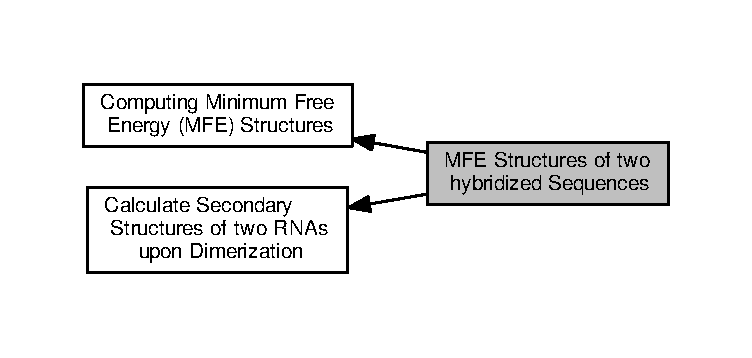
\includegraphics[width=350pt]{group__mfe__cofold}
\end{center}
\end{figure}
\subsection*{Files}
\begin{DoxyCompactItemize}
\item 
file \hyperlink{cofold_8h}{cofold.\+h}
\begin{DoxyCompactList}\small\item\em M\+F\+E version of cofolding routines. \end{DoxyCompactList}\end{DoxyCompactItemize}
\subsection*{Functions}
\begin{DoxyCompactItemize}
\item 
float \hyperlink{group__mfe__cofold_ga45515db181f17653ef7ef5487ef36d08}{vrna\+\_\+cofold} (const char $\ast$string, char $\ast$structure)
\begin{DoxyCompactList}\small\item\em Compute Minimum Free Energy (M\+F\+E), and a corresponding secondary structure for two dimerized R\+N\+A sequences. \end{DoxyCompactList}\item 
float \hyperlink{group__mfe__cofold_gabc8517f22cfe70595ee81fc837910d52}{cofold} (const char $\ast$sequence, char $\ast$structure)
\begin{DoxyCompactList}\small\item\em Compute the minimum free energy of two interacting R\+N\+A molecules. \end{DoxyCompactList}\item 
float \hyperlink{group__mfe__cofold_ga7612cfeeb1b793f1e4179b1eb53df1f3}{cofold\+\_\+par} (const char $\ast$string, char $\ast$structure, \hyperlink{group__energy__parameters_ga8a69ca7d787e4fd6079914f5343a1f35}{vrna\+\_\+param\+\_\+t} $\ast$parameters, int is\+\_\+constrained)
\begin{DoxyCompactList}\small\item\em Compute the minimum free energy of two interacting R\+N\+A molecules. \end{DoxyCompactList}\item 
void \hyperlink{group__mfe__cofold_gaafb33d7473eb9af9d1b168ca8761c41a}{free\+\_\+co\+\_\+arrays} (void)
\begin{DoxyCompactList}\small\item\em Free memory occupied by \hyperlink{group__mfe__cofold_gabc8517f22cfe70595ee81fc837910d52}{cofold()} \end{DoxyCompactList}\item 
void \hyperlink{group__mfe__cofold_ga4fcbf34e77b99bfbb2333d2ab0c41a57}{update\+\_\+cofold\+\_\+params} (void)
\begin{DoxyCompactList}\small\item\em Recalculate parameters. \end{DoxyCompactList}\item 
void \hyperlink{group__mfe__cofold_gaaadbd28b4e428710529ab4098fdacad3}{update\+\_\+cofold\+\_\+params\+\_\+par} (\hyperlink{group__energy__parameters_ga8a69ca7d787e4fd6079914f5343a1f35}{vrna\+\_\+param\+\_\+t} $\ast$parameters)
\begin{DoxyCompactList}\small\item\em Recalculate parameters. \end{DoxyCompactList}\item 
void \hyperlink{group__mfe__cofold_ga5f5bf4df35d0554f6ace9579f8744c48}{export\+\_\+cofold\+\_\+arrays\+\_\+gq} (int $\ast$$\ast$f5\+\_\+p, int $\ast$$\ast$c\+\_\+p, int $\ast$$\ast$f\+M\+L\+\_\+p, int $\ast$$\ast$f\+M1\+\_\+p, int $\ast$$\ast$fc\+\_\+p, int $\ast$$\ast$ggg\+\_\+p, int $\ast$$\ast$indx\+\_\+p, char $\ast$$\ast$ptype\+\_\+p)
\begin{DoxyCompactList}\small\item\em Export the arrays of partition function cofold (with gquadruplex support) \end{DoxyCompactList}\item 
void \hyperlink{group__mfe__cofold_ga5cb6b59983f1f74ccc00b9b9c4e84482}{export\+\_\+cofold\+\_\+arrays} (int $\ast$$\ast$f5\+\_\+p, int $\ast$$\ast$c\+\_\+p, int $\ast$$\ast$f\+M\+L\+\_\+p, int $\ast$$\ast$f\+M1\+\_\+p, int $\ast$$\ast$fc\+\_\+p, int $\ast$$\ast$indx\+\_\+p, char $\ast$$\ast$ptype\+\_\+p)
\begin{DoxyCompactList}\small\item\em Export the arrays of partition function cofold. \end{DoxyCompactList}\item 
void \hyperlink{group__mfe__cofold_ga4958b517c613e4d2afd5bce6c1060a79}{get\+\_\+monomere\+\_\+mfes} (float $\ast$e1, float $\ast$e2)
\begin{DoxyCompactList}\small\item\em get\+\_\+monomer\+\_\+free\+\_\+energies \end{DoxyCompactList}\item 
void \hyperlink{group__mfe__cofold_gafee0c32208aa2ac97338b6e3fbad7fa5}{initialize\+\_\+cofold} (int length)
\item 
float \hyperlink{group__mfe__cofold_gaab22d10c1190f205f16a77cab9d5d3ee}{vrna\+\_\+mfe\+\_\+dimer} (\hyperlink{group__fold__compound_ga1b0cef17fd40466cef5968eaeeff6166}{vrna\+\_\+fold\+\_\+compound\+\_\+t} $\ast$vc, char $\ast$structure)
\begin{DoxyCompactList}\small\item\em Compute the minimum free energy of two interacting R\+N\+A molecules. \end{DoxyCompactList}\end{DoxyCompactItemize}


\subsection{Detailed Description}


\subsection{Function Documentation}
\hypertarget{group__mfe__cofold_ga45515db181f17653ef7ef5487ef36d08}{}\index{M\+F\+E Structures of two hybridized Sequences@{M\+F\+E Structures of two hybridized Sequences}!vrna\+\_\+cofold@{vrna\+\_\+cofold}}
\index{vrna\+\_\+cofold@{vrna\+\_\+cofold}!M\+F\+E Structures of two hybridized Sequences@{M\+F\+E Structures of two hybridized Sequences}}
\subsubsection[{vrna\+\_\+cofold}]{\setlength{\rightskip}{0pt plus 5cm}float vrna\+\_\+cofold (
\begin{DoxyParamCaption}
\item[{const char $\ast$}]{string, }
\item[{char $\ast$}]{structure}
\end{DoxyParamCaption}
)}\label{group__mfe__cofold_ga45515db181f17653ef7ef5487ef36d08}


{\ttfamily \#include $<$\hyperlink{cofold_8h}{Vienna\+R\+N\+A/cofold.\+h}$>$}



Compute Minimum Free Energy (M\+F\+E), and a corresponding secondary structure for two dimerized R\+N\+A sequences. 

This simplified interface to \hyperlink{group__mfe__fold_gabd3b147371ccf25c577f88bbbaf159fd}{vrna\+\_\+mfe()} computes the M\+F\+E and, if required, a secondary structure for two R\+N\+A sequences upon dimerization using default options. Memory required for dynamic programming (D\+P) matrices will be allocated and free\textquotesingle{}d on-\/the-\/fly. Hence, after return of this function, the recursively filled matrices are not available any more for any post-\/processing, e.\+g. suboptimal backtracking, etc.

\begin{DoxyNote}{Note}
In case you want to use the filled D\+P matrices for any subsequent post-\/processing step, or you require other conditions than specified by the default model details, use \hyperlink{group__mfe__fold_gabd3b147371ccf25c577f88bbbaf159fd}{vrna\+\_\+mfe()}, and the data structure \hyperlink{group__fold__compound_ga1b0cef17fd40466cef5968eaeeff6166}{vrna\+\_\+fold\+\_\+compound\+\_\+t} instead.
\end{DoxyNote}
\begin{DoxySeeAlso}{See also}
\hyperlink{group__mfe__cofold_gaab22d10c1190f205f16a77cab9d5d3ee}{vrna\+\_\+mfe\+\_\+dimer()}, \hyperlink{group__fold__compound_ga6601d994ba32b11511b36f68b08403be}{vrna\+\_\+fold\+\_\+compound()}, \hyperlink{group__fold__compound_ga1b0cef17fd40466cef5968eaeeff6166}{vrna\+\_\+fold\+\_\+compound\+\_\+t}, \hyperlink{group__string__utils_ga74f05ece32ea73b59f84a7452afd5fae}{vrna\+\_\+cut\+\_\+point\+\_\+insert()}
\end{DoxySeeAlso}

\begin{DoxyParams}{Parameters}
{\em sequence} & two R\+N\+A sequences separated by the \textquotesingle{}\&\textquotesingle{} character \\
\hline
{\em structure} & A pointer to the character array where the secondary structure in dot-\/bracket notation will be written to \\
\hline
\end{DoxyParams}
\begin{DoxyReturn}{Returns}
the minimum free energy (M\+F\+E) in kcal/mol 
\end{DoxyReturn}
\hypertarget{group__mfe__cofold_gabc8517f22cfe70595ee81fc837910d52}{}\index{M\+F\+E Structures of two hybridized Sequences@{M\+F\+E Structures of two hybridized Sequences}!cofold@{cofold}}
\index{cofold@{cofold}!M\+F\+E Structures of two hybridized Sequences@{M\+F\+E Structures of two hybridized Sequences}}
\subsubsection[{cofold}]{\setlength{\rightskip}{0pt plus 5cm}float cofold (
\begin{DoxyParamCaption}
\item[{const char $\ast$}]{sequence, }
\item[{char $\ast$}]{structure}
\end{DoxyParamCaption}
)}\label{group__mfe__cofold_gabc8517f22cfe70595ee81fc837910d52}


{\ttfamily \#include $<$\hyperlink{cofold_8h}{Vienna\+R\+N\+A/cofold.\+h}$>$}



Compute the minimum free energy of two interacting R\+N\+A molecules. 

The code is analog to the \hyperlink{group__mfe__fold__single_gaadafcb0f140795ae62e5ca027e335a9b}{fold()} function. If \hyperlink{fold__vars_8h_ab9b2c3a37a5516614c06d0ab54b97cda}{cut\+\_\+point} ==-\/1 results should be the same as with \hyperlink{group__mfe__fold__single_gaadafcb0f140795ae62e5ca027e335a9b}{fold()}.

\begin{DoxyRefDesc}{Deprecated}
\item[\hyperlink{deprecated__deprecated000030}{Deprecated}]use \hyperlink{group__mfe__cofold_gaab22d10c1190f205f16a77cab9d5d3ee}{vrna\+\_\+mfe\+\_\+dimer()} instead\end{DoxyRefDesc}



\begin{DoxyParams}{Parameters}
{\em sequence} & The two sequences concatenated \\
\hline
{\em structure} & Will hold the barcket dot structure of the dimer molecule \\
\hline
\end{DoxyParams}
\begin{DoxyReturn}{Returns}
minimum free energy of the structure 
\end{DoxyReturn}
\hypertarget{group__mfe__cofold_ga7612cfeeb1b793f1e4179b1eb53df1f3}{}\index{M\+F\+E Structures of two hybridized Sequences@{M\+F\+E Structures of two hybridized Sequences}!cofold\+\_\+par@{cofold\+\_\+par}}
\index{cofold\+\_\+par@{cofold\+\_\+par}!M\+F\+E Structures of two hybridized Sequences@{M\+F\+E Structures of two hybridized Sequences}}
\subsubsection[{cofold\+\_\+par}]{\setlength{\rightskip}{0pt plus 5cm}float cofold\+\_\+par (
\begin{DoxyParamCaption}
\item[{const char $\ast$}]{string, }
\item[{char $\ast$}]{structure, }
\item[{{\bf vrna\+\_\+param\+\_\+t} $\ast$}]{parameters, }
\item[{int}]{is\+\_\+constrained}
\end{DoxyParamCaption}
)}\label{group__mfe__cofold_ga7612cfeeb1b793f1e4179b1eb53df1f3}


{\ttfamily \#include $<$\hyperlink{cofold_8h}{Vienna\+R\+N\+A/cofold.\+h}$>$}



Compute the minimum free energy of two interacting R\+N\+A molecules. 

\begin{DoxyRefDesc}{Deprecated}
\item[\hyperlink{deprecated__deprecated000031}{Deprecated}]use \hyperlink{group__mfe__cofold_gaab22d10c1190f205f16a77cab9d5d3ee}{vrna\+\_\+mfe\+\_\+dimer()} instead\end{DoxyRefDesc}
\hypertarget{group__mfe__cofold_gaafb33d7473eb9af9d1b168ca8761c41a}{}\index{M\+F\+E Structures of two hybridized Sequences@{M\+F\+E Structures of two hybridized Sequences}!free\+\_\+co\+\_\+arrays@{free\+\_\+co\+\_\+arrays}}
\index{free\+\_\+co\+\_\+arrays@{free\+\_\+co\+\_\+arrays}!M\+F\+E Structures of two hybridized Sequences@{M\+F\+E Structures of two hybridized Sequences}}
\subsubsection[{free\+\_\+co\+\_\+arrays}]{\setlength{\rightskip}{0pt plus 5cm}void free\+\_\+co\+\_\+arrays (
\begin{DoxyParamCaption}
\item[{void}]{}
\end{DoxyParamCaption}
)}\label{group__mfe__cofold_gaafb33d7473eb9af9d1b168ca8761c41a}


{\ttfamily \#include $<$\hyperlink{cofold_8h}{Vienna\+R\+N\+A/cofold.\+h}$>$}



Free memory occupied by \hyperlink{group__mfe__cofold_gabc8517f22cfe70595ee81fc837910d52}{cofold()} 

\begin{DoxyRefDesc}{Deprecated}
\item[\hyperlink{deprecated__deprecated000032}{Deprecated}]This function will only free memory allocated by a prior call of \hyperlink{group__mfe__cofold_gabc8517f22cfe70595ee81fc837910d52}{cofold()} or \hyperlink{group__mfe__cofold_ga7612cfeeb1b793f1e4179b1eb53df1f3}{cofold\+\_\+par()}. See \hyperlink{group__mfe__cofold_gaab22d10c1190f205f16a77cab9d5d3ee}{vrna\+\_\+mfe\+\_\+dimer()} for how to use the new A\+P\+I\end{DoxyRefDesc}


\begin{DoxyNote}{Note}
folding matrices now reside in the fold compound, and should be free\textquotesingle{}d there 
\end{DoxyNote}
\begin{DoxySeeAlso}{See also}
vrna\+\_\+fc\+\_\+destroy(), \hyperlink{group__mfe__cofold_gaab22d10c1190f205f16a77cab9d5d3ee}{vrna\+\_\+mfe\+\_\+dimer()} 
\end{DoxySeeAlso}
\hypertarget{group__mfe__cofold_ga4fcbf34e77b99bfbb2333d2ab0c41a57}{}\index{M\+F\+E Structures of two hybridized Sequences@{M\+F\+E Structures of two hybridized Sequences}!update\+\_\+cofold\+\_\+params@{update\+\_\+cofold\+\_\+params}}
\index{update\+\_\+cofold\+\_\+params@{update\+\_\+cofold\+\_\+params}!M\+F\+E Structures of two hybridized Sequences@{M\+F\+E Structures of two hybridized Sequences}}
\subsubsection[{update\+\_\+cofold\+\_\+params}]{\setlength{\rightskip}{0pt plus 5cm}void update\+\_\+cofold\+\_\+params (
\begin{DoxyParamCaption}
\item[{void}]{}
\end{DoxyParamCaption}
)}\label{group__mfe__cofold_ga4fcbf34e77b99bfbb2333d2ab0c41a57}


{\ttfamily \#include $<$\hyperlink{cofold_8h}{Vienna\+R\+N\+A/cofold.\+h}$>$}



Recalculate parameters. 

\begin{DoxyRefDesc}{Deprecated}
\item[\hyperlink{deprecated__deprecated000033}{Deprecated}]See \hyperlink{group__energy__parameters_ga5d1909208f7ea3baa98b75afaa1f62ca}{vrna\+\_\+params\+\_\+subst()} for an alternative using the new A\+P\+I \end{DoxyRefDesc}
\hypertarget{group__mfe__cofold_gaaadbd28b4e428710529ab4098fdacad3}{}\index{M\+F\+E Structures of two hybridized Sequences@{M\+F\+E Structures of two hybridized Sequences}!update\+\_\+cofold\+\_\+params\+\_\+par@{update\+\_\+cofold\+\_\+params\+\_\+par}}
\index{update\+\_\+cofold\+\_\+params\+\_\+par@{update\+\_\+cofold\+\_\+params\+\_\+par}!M\+F\+E Structures of two hybridized Sequences@{M\+F\+E Structures of two hybridized Sequences}}
\subsubsection[{update\+\_\+cofold\+\_\+params\+\_\+par}]{\setlength{\rightskip}{0pt plus 5cm}void update\+\_\+cofold\+\_\+params\+\_\+par (
\begin{DoxyParamCaption}
\item[{{\bf vrna\+\_\+param\+\_\+t} $\ast$}]{parameters}
\end{DoxyParamCaption}
)}\label{group__mfe__cofold_gaaadbd28b4e428710529ab4098fdacad3}


{\ttfamily \#include $<$\hyperlink{cofold_8h}{Vienna\+R\+N\+A/cofold.\+h}$>$}



Recalculate parameters. 

\begin{DoxyRefDesc}{Deprecated}
\item[\hyperlink{deprecated__deprecated000034}{Deprecated}]See \hyperlink{group__energy__parameters_ga5d1909208f7ea3baa98b75afaa1f62ca}{vrna\+\_\+params\+\_\+subst()} for an alternative using the new A\+P\+I \end{DoxyRefDesc}
\hypertarget{group__mfe__cofold_ga5f5bf4df35d0554f6ace9579f8744c48}{}\index{M\+F\+E Structures of two hybridized Sequences@{M\+F\+E Structures of two hybridized Sequences}!export\+\_\+cofold\+\_\+arrays\+\_\+gq@{export\+\_\+cofold\+\_\+arrays\+\_\+gq}}
\index{export\+\_\+cofold\+\_\+arrays\+\_\+gq@{export\+\_\+cofold\+\_\+arrays\+\_\+gq}!M\+F\+E Structures of two hybridized Sequences@{M\+F\+E Structures of two hybridized Sequences}}
\subsubsection[{export\+\_\+cofold\+\_\+arrays\+\_\+gq}]{\setlength{\rightskip}{0pt plus 5cm}void export\+\_\+cofold\+\_\+arrays\+\_\+gq (
\begin{DoxyParamCaption}
\item[{int $\ast$$\ast$}]{f5\+\_\+p, }
\item[{int $\ast$$\ast$}]{c\+\_\+p, }
\item[{int $\ast$$\ast$}]{f\+M\+L\+\_\+p, }
\item[{int $\ast$$\ast$}]{f\+M1\+\_\+p, }
\item[{int $\ast$$\ast$}]{fc\+\_\+p, }
\item[{int $\ast$$\ast$}]{ggg\+\_\+p, }
\item[{int $\ast$$\ast$}]{indx\+\_\+p, }
\item[{char $\ast$$\ast$}]{ptype\+\_\+p}
\end{DoxyParamCaption}
)}\label{group__mfe__cofold_ga5f5bf4df35d0554f6ace9579f8744c48}


{\ttfamily \#include $<$\hyperlink{cofold_8h}{Vienna\+R\+N\+A/cofold.\+h}$>$}



Export the arrays of partition function cofold (with gquadruplex support) 

Export the cofold arrays for use e.\+g. in the concentration Computations or suboptimal secondary structure backtracking

\begin{DoxyRefDesc}{Deprecated}
\item[\hyperlink{deprecated__deprecated000035}{Deprecated}]folding matrices now reside within the fold compound. Thus, this function will only work in conjunction with a prior call to \hyperlink{group__mfe__cofold_gabc8517f22cfe70595ee81fc837910d52}{cofold()} or \hyperlink{group__mfe__cofold_ga7612cfeeb1b793f1e4179b1eb53df1f3}{cofold\+\_\+par()}\end{DoxyRefDesc}


\begin{DoxySeeAlso}{See also}
\hyperlink{group__mfe__cofold_gaab22d10c1190f205f16a77cab9d5d3ee}{vrna\+\_\+mfe\+\_\+dimer()} for the new A\+P\+I
\end{DoxySeeAlso}

\begin{DoxyParams}{Parameters}
{\em f5\+\_\+p} & A pointer to the \textquotesingle{}f5\textquotesingle{} array, i.\+e. array conatining best free energy in interval \mbox{[}1,j\mbox{]} \\
\hline
{\em c\+\_\+p} & A pointer to the \textquotesingle{}c\textquotesingle{} array, i.\+e. array containing best free energy in interval \mbox{[}i,j\mbox{]} given that i pairs with j \\
\hline
{\em f\+M\+L\+\_\+p} & A pointer to the \textquotesingle{}M\textquotesingle{} array, i.\+e. array containing best free energy in interval \mbox{[}i,j\mbox{]} for any multiloop segment with at least one stem \\
\hline
{\em f\+M1\+\_\+p} & A pointer to the \textquotesingle{}M1\textquotesingle{} array, i.\+e. array containing best free energy in interval \mbox{[}i,j\mbox{]} for multiloop segment with exactly one stem \\
\hline
{\em fc\+\_\+p} & A pointer to the \textquotesingle{}fc\textquotesingle{} array, i.\+e. array ... \\
\hline
{\em ggg\+\_\+p} & A pointer to the \textquotesingle{}ggg\textquotesingle{} array, i.\+e. array containing best free energy of a gquadruplex delimited by \mbox{[}i,j\mbox{]} \\
\hline
{\em indx\+\_\+p} & A pointer to the indexing array used for accessing the energy matrices \\
\hline
{\em ptype\+\_\+p} & A pointer to the ptype array containing the base pair types for each possibility (i,j) \\
\hline
\end{DoxyParams}
\hypertarget{group__mfe__cofold_ga5cb6b59983f1f74ccc00b9b9c4e84482}{}\index{M\+F\+E Structures of two hybridized Sequences@{M\+F\+E Structures of two hybridized Sequences}!export\+\_\+cofold\+\_\+arrays@{export\+\_\+cofold\+\_\+arrays}}
\index{export\+\_\+cofold\+\_\+arrays@{export\+\_\+cofold\+\_\+arrays}!M\+F\+E Structures of two hybridized Sequences@{M\+F\+E Structures of two hybridized Sequences}}
\subsubsection[{export\+\_\+cofold\+\_\+arrays}]{\setlength{\rightskip}{0pt plus 5cm}void export\+\_\+cofold\+\_\+arrays (
\begin{DoxyParamCaption}
\item[{int $\ast$$\ast$}]{f5\+\_\+p, }
\item[{int $\ast$$\ast$}]{c\+\_\+p, }
\item[{int $\ast$$\ast$}]{f\+M\+L\+\_\+p, }
\item[{int $\ast$$\ast$}]{f\+M1\+\_\+p, }
\item[{int $\ast$$\ast$}]{fc\+\_\+p, }
\item[{int $\ast$$\ast$}]{indx\+\_\+p, }
\item[{char $\ast$$\ast$}]{ptype\+\_\+p}
\end{DoxyParamCaption}
)}\label{group__mfe__cofold_ga5cb6b59983f1f74ccc00b9b9c4e84482}


{\ttfamily \#include $<$\hyperlink{cofold_8h}{Vienna\+R\+N\+A/cofold.\+h}$>$}



Export the arrays of partition function cofold. 

Export the cofold arrays for use e.\+g. in the concentration Computations or suboptimal secondary structure backtracking

\begin{DoxyRefDesc}{Deprecated}
\item[\hyperlink{deprecated__deprecated000036}{Deprecated}]folding matrices now reside within the \hyperlink{group__fold__compound_ga1b0cef17fd40466cef5968eaeeff6166}{vrna\+\_\+fold\+\_\+compound\+\_\+t}. Thus, this function will only work in conjunction with a prior call to the deprecated functions \hyperlink{group__mfe__cofold_gabc8517f22cfe70595ee81fc837910d52}{cofold()} or \hyperlink{group__mfe__cofold_ga7612cfeeb1b793f1e4179b1eb53df1f3}{cofold\+\_\+par()}\end{DoxyRefDesc}


\begin{DoxySeeAlso}{See also}
\hyperlink{group__mfe__cofold_gaab22d10c1190f205f16a77cab9d5d3ee}{vrna\+\_\+mfe\+\_\+dimer()} for the new A\+P\+I
\end{DoxySeeAlso}

\begin{DoxyParams}{Parameters}
{\em f5\+\_\+p} & A pointer to the \textquotesingle{}f5\textquotesingle{} array, i.\+e. array conatining best free energy in interval \mbox{[}1,j\mbox{]} \\
\hline
{\em c\+\_\+p} & A pointer to the \textquotesingle{}c\textquotesingle{} array, i.\+e. array containing best free energy in interval \mbox{[}i,j\mbox{]} given that i pairs with j \\
\hline
{\em f\+M\+L\+\_\+p} & A pointer to the \textquotesingle{}M\textquotesingle{} array, i.\+e. array containing best free energy in interval \mbox{[}i,j\mbox{]} for any multiloop segment with at least one stem \\
\hline
{\em f\+M1\+\_\+p} & A pointer to the \textquotesingle{}M1\textquotesingle{} array, i.\+e. array containing best free energy in interval \mbox{[}i,j\mbox{]} for multiloop segment with exactly one stem \\
\hline
{\em fc\+\_\+p} & A pointer to the \textquotesingle{}fc\textquotesingle{} array, i.\+e. array ... \\
\hline
{\em indx\+\_\+p} & A pointer to the indexing array used for accessing the energy matrices \\
\hline
{\em ptype\+\_\+p} & A pointer to the ptype array containing the base pair types for each possibility (i,j) \\
\hline
\end{DoxyParams}
\hypertarget{group__mfe__cofold_ga4958b517c613e4d2afd5bce6c1060a79}{}\index{M\+F\+E Structures of two hybridized Sequences@{M\+F\+E Structures of two hybridized Sequences}!get\+\_\+monomere\+\_\+mfes@{get\+\_\+monomere\+\_\+mfes}}
\index{get\+\_\+monomere\+\_\+mfes@{get\+\_\+monomere\+\_\+mfes}!M\+F\+E Structures of two hybridized Sequences@{M\+F\+E Structures of two hybridized Sequences}}
\subsubsection[{get\+\_\+monomere\+\_\+mfes}]{\setlength{\rightskip}{0pt plus 5cm}void get\+\_\+monomere\+\_\+mfes (
\begin{DoxyParamCaption}
\item[{float $\ast$}]{e1, }
\item[{float $\ast$}]{e2}
\end{DoxyParamCaption}
)}\label{group__mfe__cofold_ga4958b517c613e4d2afd5bce6c1060a79}


{\ttfamily \#include $<$\hyperlink{cofold_8h}{Vienna\+R\+N\+A/cofold.\+h}$>$}



get\+\_\+monomer\+\_\+free\+\_\+energies 

Export monomer free energies out of cofold arrays \begin{DoxyRefDesc}{Deprecated}
\item[\hyperlink{deprecated__deprecated000037}{Deprecated}]\{This function is obsolete and will be removed soon!\}\end{DoxyRefDesc}



\begin{DoxyParams}{Parameters}
{\em e1} & A pointer to a variable where the energy of molecule A will be written to \\
\hline
{\em e2} & A pointer to a variable where the energy of molecule B will be written to \\
\hline
\end{DoxyParams}
\hypertarget{group__mfe__cofold_gafee0c32208aa2ac97338b6e3fbad7fa5}{}\index{M\+F\+E Structures of two hybridized Sequences@{M\+F\+E Structures of two hybridized Sequences}!initialize\+\_\+cofold@{initialize\+\_\+cofold}}
\index{initialize\+\_\+cofold@{initialize\+\_\+cofold}!M\+F\+E Structures of two hybridized Sequences@{M\+F\+E Structures of two hybridized Sequences}}
\subsubsection[{initialize\+\_\+cofold}]{\setlength{\rightskip}{0pt plus 5cm}void initialize\+\_\+cofold (
\begin{DoxyParamCaption}
\item[{int}]{length}
\end{DoxyParamCaption}
)}\label{group__mfe__cofold_gafee0c32208aa2ac97338b6e3fbad7fa5}


{\ttfamily \#include $<$\hyperlink{cofold_8h}{Vienna\+R\+N\+A/cofold.\+h}$>$}

allocate arrays for folding \begin{DoxyRefDesc}{Deprecated}
\item[\hyperlink{deprecated__deprecated000038}{Deprecated}]\{This function is obsolete and will be removed soon!\} \end{DoxyRefDesc}
\hypertarget{group__mfe__cofold_gaab22d10c1190f205f16a77cab9d5d3ee}{}\index{M\+F\+E Structures of two hybridized Sequences@{M\+F\+E Structures of two hybridized Sequences}!vrna\+\_\+mfe\+\_\+dimer@{vrna\+\_\+mfe\+\_\+dimer}}
\index{vrna\+\_\+mfe\+\_\+dimer@{vrna\+\_\+mfe\+\_\+dimer}!M\+F\+E Structures of two hybridized Sequences@{M\+F\+E Structures of two hybridized Sequences}}
\subsubsection[{vrna\+\_\+mfe\+\_\+dimer}]{\setlength{\rightskip}{0pt plus 5cm}float vrna\+\_\+mfe\+\_\+dimer (
\begin{DoxyParamCaption}
\item[{{\bf vrna\+\_\+fold\+\_\+compound\+\_\+t} $\ast$}]{vc, }
\item[{char $\ast$}]{structure}
\end{DoxyParamCaption}
)}\label{group__mfe__cofold_gaab22d10c1190f205f16a77cab9d5d3ee}


{\ttfamily \#include $<$\hyperlink{mfe_8h}{Vienna\+R\+N\+A/mfe.\+h}$>$}



Compute the minimum free energy of two interacting R\+N\+A molecules. 

The code is analog to the \hyperlink{group__mfe__fold_gabd3b147371ccf25c577f88bbbaf159fd}{vrna\+\_\+mfe()} function.


\begin{DoxyParams}{Parameters}
{\em vc} & fold compound \\
\hline
{\em structure} & Will hold the barcket dot structure of the dimer molecule \\
\hline
\end{DoxyParams}
\begin{DoxyReturn}{Returns}
minimum free energy of the structure 
\end{DoxyReturn}

\hypertarget{group__pf__cofold}{}\section{Partition Function for two hybridized Sequences}
\label{group__pf__cofold}\index{Partition Function for two hybridized Sequences@{Partition Function for two hybridized Sequences}}


Partition Function Cofolding.  


Collaboration diagram for Partition Function for two hybridized Sequences\+:
\nopagebreak
\begin{figure}[H]
\begin{center}
\leavevmode
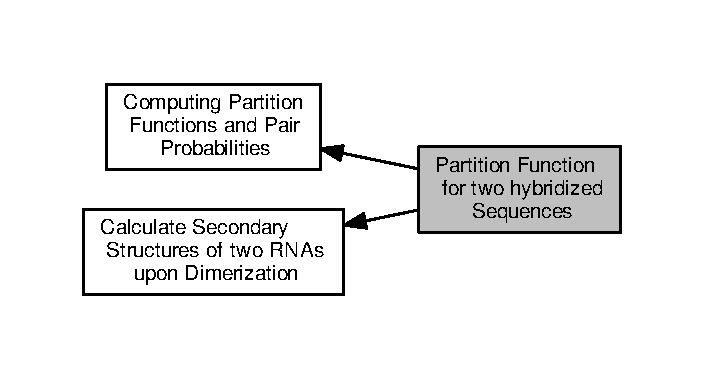
\includegraphics[width=338pt]{group__pf__cofold}
\end{center}
\end{figure}
\subsection*{Files}
\begin{DoxyCompactItemize}
\item 
file \hyperlink{part__func__co_8h}{part\+\_\+func\+\_\+co.\+h}
\begin{DoxyCompactList}\small\item\em Partition function for two R\+N\+A sequences. \end{DoxyCompactList}\end{DoxyCompactItemize}
\subsection*{Data Structures}
\begin{DoxyCompactItemize}
\item 
struct \hyperlink{group__pf__cofold_structvrna__dimer__pf__s}{vrna\+\_\+dimer\+\_\+pf\+\_\+s}
\item 
struct \hyperlink{group__pf__cofold_structvrna__dimer__conc__s}{vrna\+\_\+dimer\+\_\+conc\+\_\+s}
\end{DoxyCompactItemize}
\subsection*{Typedefs}
\begin{DoxyCompactItemize}
\item 
\hypertarget{group__pf__cofold_ga444df1587c9a2ca15b8eb25188f629c3}{}typedef struct \hyperlink{group__pf__cofold_structvrna__dimer__pf__s}{vrna\+\_\+dimer\+\_\+pf\+\_\+s} \hyperlink{group__pf__cofold_ga444df1587c9a2ca15b8eb25188f629c3}{vrna\+\_\+dimer\+\_\+pf\+\_\+t}\label{group__pf__cofold_ga444df1587c9a2ca15b8eb25188f629c3}

\begin{DoxyCompactList}\small\item\em Typename for the data structure that stores the dimer partition functions, \hyperlink{group__pf__cofold_structvrna__dimer__pf__s}{vrna\+\_\+dimer\+\_\+pf\+\_\+s}, as returned by \hyperlink{group__pf__cofold_ga4e5c7d06c302a7c59fc0d64dc142ca63}{vrna\+\_\+pf\+\_\+dimer()} \end{DoxyCompactList}\item 
\hypertarget{group__pf__cofold_gac48c2723444ecfdceafcfd525ca98322}{}typedef struct \hyperlink{group__pf__cofold_structvrna__dimer__conc__s}{vrna\+\_\+dimer\+\_\+conc\+\_\+s} \hyperlink{group__pf__cofold_gac48c2723444ecfdceafcfd525ca98322}{vrna\+\_\+dimer\+\_\+conc\+\_\+t}\label{group__pf__cofold_gac48c2723444ecfdceafcfd525ca98322}

\begin{DoxyCompactList}\small\item\em Typename for the data structure that stores the dimer concentrations, \hyperlink{group__pf__cofold_structvrna__dimer__conc__s}{vrna\+\_\+dimer\+\_\+conc\+\_\+s}, as required by vrna\+\_\+pf\+\_\+dimer\+\_\+concentration() \end{DoxyCompactList}\end{DoxyCompactItemize}
\subsection*{Functions}
\begin{DoxyCompactItemize}
\item 
\hyperlink{group__pf__cofold_ga444df1587c9a2ca15b8eb25188f629c3}{vrna\+\_\+dimer\+\_\+pf\+\_\+t} \hyperlink{group__pf__cofold_ga4e5c7d06c302a7c59fc0d64dc142ca63}{vrna\+\_\+pf\+\_\+dimer} (\hyperlink{group__fold__compound_ga1b0cef17fd40466cef5968eaeeff6166}{vrna\+\_\+fold\+\_\+compound\+\_\+t} $\ast$vc, char $\ast$structure)
\begin{DoxyCompactList}\small\item\em Calculate partition function and base pair probabilities of nucleic acid/nucleic acid dimers. \end{DoxyCompactList}\item 
void \hyperlink{group__pf__cofold_gaf04708a63d2385d5959db9f886741479}{vrna\+\_\+pf\+\_\+dimer\+\_\+probs} (double F\+A\+B, double F\+A, double F\+B, \hyperlink{group__data__structures_ga8e4eb5e1bfc95776559575beb359af87}{vrna\+\_\+plist\+\_\+t} $\ast$pr\+A\+B, const \hyperlink{group__data__structures_ga8e4eb5e1bfc95776559575beb359af87}{vrna\+\_\+plist\+\_\+t} $\ast$pr\+A, const \hyperlink{group__data__structures_ga8e4eb5e1bfc95776559575beb359af87}{vrna\+\_\+plist\+\_\+t} $\ast$pr\+B, int Alength, const \hyperlink{group__energy__parameters_ga01d8b92fe734df8d79a6169482c7d8d8}{vrna\+\_\+exp\+\_\+param\+\_\+t} $\ast$exp\+\_\+params)
\begin{DoxyCompactList}\small\item\em Compute Boltzmann probabilities of dimerization without homodimers. \end{DoxyCompactList}\item 
\hyperlink{group__pf__cofold_gac48c2723444ecfdceafcfd525ca98322}{vrna\+\_\+dimer\+\_\+conc\+\_\+t} $\ast$ \hyperlink{group__pf__cofold_ga83b8d5d0f7875d6d5013b208f23e3356}{vrna\+\_\+pf\+\_\+dimer\+\_\+concentrations} (double Fc\+A\+B, double Fc\+A\+A, double Fc\+B\+B, double F\+E\+A, double F\+E\+B, const double $\ast$startconc, const \hyperlink{group__energy__parameters_ga01d8b92fe734df8d79a6169482c7d8d8}{vrna\+\_\+exp\+\_\+param\+\_\+t} $\ast$exp\+\_\+params)
\begin{DoxyCompactList}\small\item\em Given two start monomer concentrations a and b, compute the concentrations in thermodynamic equilibrium of all dimers and the monomers. \end{DoxyCompactList}\end{DoxyCompactItemize}
\subsection*{Variables}
\begin{DoxyCompactItemize}
\item 
\hypertarget{group__pf__cofold_gaff27888c4088cc1f60fd59cbd589474c}{}int \hyperlink{group__pf__cofold_gaff27888c4088cc1f60fd59cbd589474c}{mirnatog}\label{group__pf__cofold_gaff27888c4088cc1f60fd59cbd589474c}

\begin{DoxyCompactList}\small\item\em Toggles no intrabp in 2nd mol. \end{DoxyCompactList}\item 
\hypertarget{group__pf__cofold_gac2d1851a710a8561390861155ca988fe}{}double \hyperlink{group__pf__cofold_gac2d1851a710a8561390861155ca988fe}{F\+\_\+monomer} \mbox{[}2\mbox{]}\label{group__pf__cofold_gac2d1851a710a8561390861155ca988fe}

\begin{DoxyCompactList}\small\item\em Free energies of the two monomers. \end{DoxyCompactList}\end{DoxyCompactItemize}


\subsection{Detailed Description}
Partition Function Cofolding. 

To simplify the implementation the partition function computation is done internally in a null model that does not include the duplex initiation energy, i.\+e. the entropic penalty for producing a dimer from two monomers). The resulting free energies and pair probabilities are initially relative to that null model. In a second step the free energies can be corrected to include the dimerization penalty, and the pair probabilities can be divided into the conditional pair probabilities given that a re dimer is formed or not formed. See \cite{bernhart:2006} for further details. 

\subsection{Data Structure Documentation}
\index{vrna\+\_\+dimer\+\_\+pf\+\_\+s@{vrna\+\_\+dimer\+\_\+pf\+\_\+s}}\label{structvrna__dimer__pf__s}
\hypertarget{group__pf__cofold_structvrna__dimer__pf__s}{}
\subsubsection{struct vrna\+\_\+dimer\+\_\+pf\+\_\+s}
\subsubsection*{Data Fields}
\begin{DoxyCompactItemize}
\item 
\hypertarget{group__pf__cofold_a82e31d1fb6e95923fab6036f52c370af}{}double \hyperlink{group__pf__cofold_a82e31d1fb6e95923fab6036f52c370af}{F0\+A\+B}\label{group__pf__cofold_a82e31d1fb6e95923fab6036f52c370af}

\begin{DoxyCompactList}\small\item\em Null model without Duplex\+Init. \end{DoxyCompactList}\item 
\hypertarget{group__pf__cofold_a01a87f59db2b7fbf883b056e6f6c673a}{}double \hyperlink{group__pf__cofold_a01a87f59db2b7fbf883b056e6f6c673a}{F\+A\+B}\label{group__pf__cofold_a01a87f59db2b7fbf883b056e6f6c673a}

\begin{DoxyCompactList}\small\item\em all states with Duplex\+Init correction \end{DoxyCompactList}\item 
\hypertarget{group__pf__cofold_a7b01cea5721f61badebc29cf0a9c4266}{}double \hyperlink{group__pf__cofold_a7b01cea5721f61badebc29cf0a9c4266}{Fc\+A\+B}\label{group__pf__cofold_a7b01cea5721f61badebc29cf0a9c4266}

\begin{DoxyCompactList}\small\item\em true hybrid states only \end{DoxyCompactList}\item 
\hypertarget{group__pf__cofold_a1aca57247f2c023d08028b1919005b0a}{}double \hyperlink{group__pf__cofold_a1aca57247f2c023d08028b1919005b0a}{F\+A}\label{group__pf__cofold_a1aca57247f2c023d08028b1919005b0a}

\begin{DoxyCompactList}\small\item\em monomer A \end{DoxyCompactList}\item 
\hypertarget{group__pf__cofold_ab4d307be5400604d3c1d84d58a9981df}{}double \hyperlink{group__pf__cofold_ab4d307be5400604d3c1d84d58a9981df}{F\+B}\label{group__pf__cofold_ab4d307be5400604d3c1d84d58a9981df}

\begin{DoxyCompactList}\small\item\em monomer B \end{DoxyCompactList}\end{DoxyCompactItemize}
\index{vrna\+\_\+dimer\+\_\+conc\+\_\+s@{vrna\+\_\+dimer\+\_\+conc\+\_\+s}}\label{structvrna__dimer__conc__s}
\hypertarget{group__pf__cofold_structvrna__dimer__conc__s}{}
\subsubsection{struct vrna\+\_\+dimer\+\_\+conc\+\_\+s}
\subsubsection*{Data Fields}
\begin{DoxyCompactItemize}
\item 
\hypertarget{group__pf__cofold_a9722115f1a483583beaf7ef0f8180087}{}double \hyperlink{group__pf__cofold_a9722115f1a483583beaf7ef0f8180087}{A0}\label{group__pf__cofold_a9722115f1a483583beaf7ef0f8180087}

\begin{DoxyCompactList}\small\item\em start concentration A \end{DoxyCompactList}\item 
\hypertarget{group__pf__cofold_a5231715f610413dd5a88bc9f958cf5f3}{}double \hyperlink{group__pf__cofold_a5231715f610413dd5a88bc9f958cf5f3}{B0}\label{group__pf__cofold_a5231715f610413dd5a88bc9f958cf5f3}

\begin{DoxyCompactList}\small\item\em start concentration B \end{DoxyCompactList}\item 
\hypertarget{group__pf__cofold_aef56a1fe8d7f07e7b5d9a65417dda8a4}{}double \hyperlink{group__pf__cofold_aef56a1fe8d7f07e7b5d9a65417dda8a4}{A\+Bc}\label{group__pf__cofold_aef56a1fe8d7f07e7b5d9a65417dda8a4}

\begin{DoxyCompactList}\small\item\em End concentration A\+B. \end{DoxyCompactList}\end{DoxyCompactItemize}


\subsection{Function Documentation}
\hypertarget{group__pf__cofold_ga4e5c7d06c302a7c59fc0d64dc142ca63}{}\index{Partition Function for two hybridized Sequences@{Partition Function for two hybridized Sequences}!vrna\+\_\+pf\+\_\+dimer@{vrna\+\_\+pf\+\_\+dimer}}
\index{vrna\+\_\+pf\+\_\+dimer@{vrna\+\_\+pf\+\_\+dimer}!Partition Function for two hybridized Sequences@{Partition Function for two hybridized Sequences}}
\subsubsection[{vrna\+\_\+pf\+\_\+dimer}]{\setlength{\rightskip}{0pt plus 5cm}{\bf vrna\+\_\+dimer\+\_\+pf\+\_\+t} vrna\+\_\+pf\+\_\+dimer (
\begin{DoxyParamCaption}
\item[{{\bf vrna\+\_\+fold\+\_\+compound\+\_\+t} $\ast$}]{vc, }
\item[{char $\ast$}]{structure}
\end{DoxyParamCaption}
)}\label{group__pf__cofold_ga4e5c7d06c302a7c59fc0d64dc142ca63}


{\ttfamily \#include $<$\hyperlink{part__func__co_8h}{Vienna\+R\+N\+A/part\+\_\+func\+\_\+co.\+h}$>$}



Calculate partition function and base pair probabilities of nucleic acid/nucleic acid dimers. 

This is the cofold partition function folding.

\begin{DoxySeeAlso}{See also}
\hyperlink{group__fold__compound_ga6601d994ba32b11511b36f68b08403be}{vrna\+\_\+fold\+\_\+compound()} for how to retrieve the necessary data structure
\end{DoxySeeAlso}

\begin{DoxyParams}{Parameters}
{\em vc} & the fold compound data structure \\
\hline
{\em structure} & Will hold the structure or constraints \\
\hline
\end{DoxyParams}
\begin{DoxyReturn}{Returns}
vrna\+\_\+dimer\+\_\+pf\+\_\+t structure containing a set of energies needed for concentration computations. 
\end{DoxyReturn}
\hypertarget{group__pf__cofold_gaf04708a63d2385d5959db9f886741479}{}\index{Partition Function for two hybridized Sequences@{Partition Function for two hybridized Sequences}!vrna\+\_\+pf\+\_\+dimer\+\_\+probs@{vrna\+\_\+pf\+\_\+dimer\+\_\+probs}}
\index{vrna\+\_\+pf\+\_\+dimer\+\_\+probs@{vrna\+\_\+pf\+\_\+dimer\+\_\+probs}!Partition Function for two hybridized Sequences@{Partition Function for two hybridized Sequences}}
\subsubsection[{vrna\+\_\+pf\+\_\+dimer\+\_\+probs}]{\setlength{\rightskip}{0pt plus 5cm}void vrna\+\_\+pf\+\_\+dimer\+\_\+probs (
\begin{DoxyParamCaption}
\item[{double}]{F\+A\+B, }
\item[{double}]{F\+A, }
\item[{double}]{F\+B, }
\item[{{\bf vrna\+\_\+plist\+\_\+t} $\ast$}]{pr\+A\+B, }
\item[{const {\bf vrna\+\_\+plist\+\_\+t} $\ast$}]{pr\+A, }
\item[{const {\bf vrna\+\_\+plist\+\_\+t} $\ast$}]{pr\+B, }
\item[{int}]{Alength, }
\item[{const {\bf vrna\+\_\+exp\+\_\+param\+\_\+t} $\ast$}]{exp\+\_\+params}
\end{DoxyParamCaption}
)}\label{group__pf__cofold_gaf04708a63d2385d5959db9f886741479}


{\ttfamily \#include $<$\hyperlink{part__func__co_8h}{Vienna\+R\+N\+A/part\+\_\+func\+\_\+co.\+h}$>$}



Compute Boltzmann probabilities of dimerization without homodimers. 

Given the pair probabilities and free energies (in the null model) for a dimer A\+B and the two constituent monomers A and B, compute the conditional pair probabilities given that a dimer A\+B actually forms. Null model pair probabilities are given as a list as produced by \hyperlink{group__pf__fold_gaa3bf26a0ee2e9f2225afbaee44a37264}{vrna\+\_\+plist\+\_\+from\+\_\+probs()}, the dimer probabilities \textquotesingle{}pr\+A\+B\textquotesingle{} are modified in place.


\begin{DoxyParams}{Parameters}
{\em F\+A\+B} & free energy of dimer A\+B \\
\hline
{\em F\+E\+A} & free energy of monomer A \\
\hline
{\em F\+E\+B} & free energy of monomer B \\
\hline
{\em pr\+A\+B} & pair probabilities for dimer \\
\hline
{\em pr\+A} & pair probabilities monomer \\
\hline
{\em pr\+B} & pair probabilities monomer \\
\hline
{\em Alength} & Length of molecule A \\
\hline
{\em exp\+\_\+params} & The precomputed Boltzmann factors \\
\hline
\end{DoxyParams}
\hypertarget{group__pf__cofold_ga83b8d5d0f7875d6d5013b208f23e3356}{}\index{Partition Function for two hybridized Sequences@{Partition Function for two hybridized Sequences}!vrna\+\_\+pf\+\_\+dimer\+\_\+concentrations@{vrna\+\_\+pf\+\_\+dimer\+\_\+concentrations}}
\index{vrna\+\_\+pf\+\_\+dimer\+\_\+concentrations@{vrna\+\_\+pf\+\_\+dimer\+\_\+concentrations}!Partition Function for two hybridized Sequences@{Partition Function for two hybridized Sequences}}
\subsubsection[{vrna\+\_\+pf\+\_\+dimer\+\_\+concentrations}]{\setlength{\rightskip}{0pt plus 5cm}{\bf vrna\+\_\+dimer\+\_\+conc\+\_\+t}$\ast$ vrna\+\_\+pf\+\_\+dimer\+\_\+concentrations (
\begin{DoxyParamCaption}
\item[{double}]{Fc\+A\+B, }
\item[{double}]{Fc\+A\+A, }
\item[{double}]{Fc\+B\+B, }
\item[{double}]{F\+E\+A, }
\item[{double}]{F\+E\+B, }
\item[{const double $\ast$}]{startconc, }
\item[{const {\bf vrna\+\_\+exp\+\_\+param\+\_\+t} $\ast$}]{exp\+\_\+params}
\end{DoxyParamCaption}
)}\label{group__pf__cofold_ga83b8d5d0f7875d6d5013b208f23e3356}


{\ttfamily \#include $<$\hyperlink{part__func__co_8h}{Vienna\+R\+N\+A/part\+\_\+func\+\_\+co.\+h}$>$}



Given two start monomer concentrations a and b, compute the concentrations in thermodynamic equilibrium of all dimers and the monomers. 

This function takes an array \textquotesingle{}startconc\textquotesingle{} of input concentrations with alternating entries for the initial concentrations of molecules A and B (terminated by two zeroes), then computes the resulting equilibrium concentrations from the free energies for the dimers. Dimer free energies should be the dimer-\/only free energies, i.\+e. the Fc\+A\+B entries from the \hyperlink{group__pf__cofold_ga444df1587c9a2ca15b8eb25188f629c3}{vrna\+\_\+dimer\+\_\+pf\+\_\+t} struct.


\begin{DoxyParams}{Parameters}
{\em F\+E\+A\+B} & Free energy of A\+B dimer (Fc\+A\+B entry) \\
\hline
{\em F\+E\+A\+A} & Free energy of A\+A dimer (Fc\+A\+B entry) \\
\hline
{\em F\+E\+B\+B} & Free energy of B\+B dimer (Fc\+A\+B entry) \\
\hline
{\em F\+E\+A} & Free energy of monomer A \\
\hline
{\em F\+E\+B} & Free energy of monomer B \\
\hline
{\em startconc} & List of start concentrations \mbox{[}a0\mbox{]},\mbox{[}b0\mbox{]},\mbox{[}a1\mbox{]},\mbox{[}b1\mbox{]},...,\mbox{[}an\mbox{]}\mbox{[}bn\mbox{]},\mbox{[}0\mbox{]},\mbox{[}0\mbox{]} \\
\hline
{\em exp\+\_\+params} & The precomputed Boltzmann factors \\
\hline
\end{DoxyParams}
\begin{DoxyReturn}{Returns}
vrna\+\_\+dimer\+\_\+conc\+\_\+t array containing the equilibrium energies and start concentrations 
\end{DoxyReturn}

\hypertarget{group__up__cofold}{}\section{Partition Function for two hybridized Sequences as a stepwise Process}
\label{group__up__cofold}\index{Partition Function for two hybridized Sequences as a stepwise Process@{Partition Function for two hybridized Sequences as a stepwise Process}}


Partition Function Cofolding as a stepwise process.  


Collaboration diagram for Partition Function for two hybridized Sequences as a stepwise Process\+:
\nopagebreak
\begin{figure}[H]
\begin{center}
\leavevmode
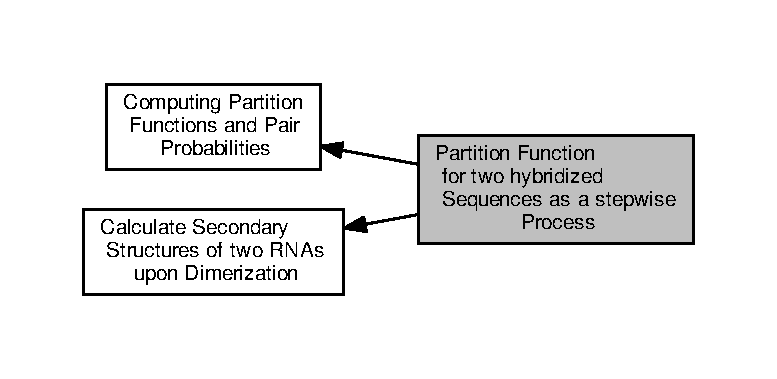
\includegraphics[width=350pt]{group__up__cofold}
\end{center}
\end{figure}
\subsection*{Files}
\begin{DoxyCompactItemize}
\item 
file \hyperlink{part__func__up_8h}{part\+\_\+func\+\_\+up.\+h}
\begin{DoxyCompactList}\small\item\em Partition Function Cofolding as stepwise process. \end{DoxyCompactList}\end{DoxyCompactItemize}
\subsection*{Functions}
\begin{DoxyCompactItemize}
\item 
\hyperlink{group__data__structures_structpu__contrib}{pu\+\_\+contrib} $\ast$ \hyperlink{group__up__cofold_ga5b4ee40e190d2f633cd01cf0d2fe93cf}{pf\+\_\+unstru} (char $\ast$sequence, int max\+\_\+w)
\begin{DoxyCompactList}\small\item\em Calculate the partition function over all unpaired regions of a maximal length. \end{DoxyCompactList}\item 
\hyperlink{group__data__structures_structinteract}{interact} $\ast$ \hyperlink{group__up__cofold_ga1aa0aa02bc3a724f87360c03097afd00}{pf\+\_\+interact} (const char $\ast$s1, const char $\ast$s2, \hyperlink{group__data__structures_structpu__contrib}{pu\+\_\+contrib} $\ast$p\+\_\+c, \hyperlink{group__data__structures_structpu__contrib}{pu\+\_\+contrib} $\ast$p\+\_\+c2, int max\+\_\+w, char $\ast$cstruc, int incr3, int incr5)
\begin{DoxyCompactList}\small\item\em Calculates the probability of a local interaction between two sequences. \end{DoxyCompactList}\item 
\hypertarget{group__up__cofold_gadde308fd5f696dc271b1532aa96fd12f}{}void \hyperlink{group__up__cofold_gadde308fd5f696dc271b1532aa96fd12f}{free\+\_\+interact} (\hyperlink{group__data__structures_structinteract}{interact} $\ast$pin)\label{group__up__cofold_gadde308fd5f696dc271b1532aa96fd12f}

\begin{DoxyCompactList}\small\item\em Frees the output of function \hyperlink{group__up__cofold_ga1aa0aa02bc3a724f87360c03097afd00}{pf\+\_\+interact()}. \end{DoxyCompactList}\item 
\hypertarget{group__up__cofold_gac20bd61824981d45ce0dc9934aa56df8}{}void \hyperlink{group__up__cofold_gac20bd61824981d45ce0dc9934aa56df8}{free\+\_\+pu\+\_\+contrib\+\_\+struct} (\hyperlink{group__data__structures_structpu__contrib}{pu\+\_\+contrib} $\ast$pu)\label{group__up__cofold_gac20bd61824981d45ce0dc9934aa56df8}

\begin{DoxyCompactList}\small\item\em Frees the output of function \hyperlink{group__up__cofold_ga5b4ee40e190d2f633cd01cf0d2fe93cf}{pf\+\_\+unstru()}. \end{DoxyCompactList}\end{DoxyCompactItemize}


\subsection{Detailed Description}
Partition Function Cofolding as a stepwise process. 



\subsection{Function Documentation}
\hypertarget{group__up__cofold_ga5b4ee40e190d2f633cd01cf0d2fe93cf}{}\index{Partition Function for two hybridized Sequences as a stepwise Process@{Partition Function for two hybridized Sequences as a stepwise Process}!pf\+\_\+unstru@{pf\+\_\+unstru}}
\index{pf\+\_\+unstru@{pf\+\_\+unstru}!Partition Function for two hybridized Sequences as a stepwise Process@{Partition Function for two hybridized Sequences as a stepwise Process}}
\subsubsection[{pf\+\_\+unstru}]{\setlength{\rightskip}{0pt plus 5cm}{\bf pu\+\_\+contrib}$\ast$ pf\+\_\+unstru (
\begin{DoxyParamCaption}
\item[{char $\ast$}]{sequence, }
\item[{int}]{max\+\_\+w}
\end{DoxyParamCaption}
)}\label{group__up__cofold_ga5b4ee40e190d2f633cd01cf0d2fe93cf}


{\ttfamily \#include $<$\hyperlink{part__func__up_8h}{Vienna\+R\+N\+A/part\+\_\+func\+\_\+up.\+h}$>$}



Calculate the partition function over all unpaired regions of a maximal length. 

You have to call function \hyperlink{group__pf__fold_gadc3db3d98742427e7001a7fd36ef28c2}{pf\+\_\+fold()} providing the same sequence before calling \hyperlink{group__up__cofold_ga5b4ee40e190d2f633cd01cf0d2fe93cf}{pf\+\_\+unstru()}. If you want to calculate unpaired regions for a constrained structure, set variable \textquotesingle{}structure\textquotesingle{} in function \textquotesingle{}\hyperlink{group__pf__fold_gadc3db3d98742427e7001a7fd36ef28c2}{pf\+\_\+fold()}\textquotesingle{} to the constrain string. It returns a \hyperlink{group__data__structures_structpu__contrib}{pu\+\_\+contrib} struct containing four arrays of dimension \mbox{[}i = 1 to length(sequence)\mbox{]}\mbox{[}j = 0 to u-\/1\mbox{]} containing all possible contributions to the probabilities of unpaired regions of maximum length u. Each array in \hyperlink{group__data__structures_structpu__contrib}{pu\+\_\+contrib} contains one of the contributions to the total probability of being unpaired\+: The probability of being unpaired within an exterior loop is in array \hyperlink{group__data__structures_structpu__contrib}{pu\+\_\+contrib}-\/$>$E, the probability of being unpaired within a hairpin loop is in array \hyperlink{group__data__structures_structpu__contrib}{pu\+\_\+contrib}-\/$>$H, the probability of being unpaired within an interior loop is in array \hyperlink{group__data__structures_structpu__contrib}{pu\+\_\+contrib}-\/$>$I and probability of being unpaired within a multi-\/loop is in array \hyperlink{group__data__structures_structpu__contrib}{pu\+\_\+contrib}-\/$>$M. The total probability of being unpaired is the sum of the four arrays of \hyperlink{group__data__structures_structpu__contrib}{pu\+\_\+contrib}.

This function frees everything allocated automatically. To free the output structure call free\+\_\+pu\+\_\+contrib().


\begin{DoxyParams}{Parameters}
{\em sequence} & \\
\hline
{\em max\+\_\+w} & \\
\hline
\end{DoxyParams}
\begin{DoxyReturn}{Returns}

\end{DoxyReturn}
\hypertarget{group__up__cofold_ga1aa0aa02bc3a724f87360c03097afd00}{}\index{Partition Function for two hybridized Sequences as a stepwise Process@{Partition Function for two hybridized Sequences as a stepwise Process}!pf\+\_\+interact@{pf\+\_\+interact}}
\index{pf\+\_\+interact@{pf\+\_\+interact}!Partition Function for two hybridized Sequences as a stepwise Process@{Partition Function for two hybridized Sequences as a stepwise Process}}
\subsubsection[{pf\+\_\+interact}]{\setlength{\rightskip}{0pt plus 5cm}{\bf interact}$\ast$ pf\+\_\+interact (
\begin{DoxyParamCaption}
\item[{const char $\ast$}]{s1, }
\item[{const char $\ast$}]{s2, }
\item[{{\bf pu\+\_\+contrib} $\ast$}]{p\+\_\+c, }
\item[{{\bf pu\+\_\+contrib} $\ast$}]{p\+\_\+c2, }
\item[{int}]{max\+\_\+w, }
\item[{char $\ast$}]{cstruc, }
\item[{int}]{incr3, }
\item[{int}]{incr5}
\end{DoxyParamCaption}
)}\label{group__up__cofold_ga1aa0aa02bc3a724f87360c03097afd00}


{\ttfamily \#include $<$\hyperlink{part__func__up_8h}{Vienna\+R\+N\+A/part\+\_\+func\+\_\+up.\+h}$>$}



Calculates the probability of a local interaction between two sequences. 

The function considers the probability that the region of interaction is unpaired within \textquotesingle{}s1\textquotesingle{} and \textquotesingle{}s2\textquotesingle{}. The longer sequence has to be given as \textquotesingle{}s1\textquotesingle{}. The shorter sequence has to be given as \textquotesingle{}s2\textquotesingle{}. Function \hyperlink{group__up__cofold_ga5b4ee40e190d2f633cd01cf0d2fe93cf}{pf\+\_\+unstru()} has to be called for \textquotesingle{}s1\textquotesingle{} and \textquotesingle{}s2\textquotesingle{}, where the probabilities of being unpaired have to be given in \textquotesingle{}p\+\_\+c\textquotesingle{} and \textquotesingle{}p\+\_\+c2\textquotesingle{}, respectively. If you do not want to include the probabilities of being unpaired for \textquotesingle{}s2\textquotesingle{} set \textquotesingle{}p\+\_\+c2\textquotesingle{} to N\+U\+L\+L. If variable \textquotesingle{}cstruc\textquotesingle{} is not N\+U\+L\+L, constrained folding is done\+: The available constrains for intermolecular interaction are\+: \textquotesingle{}.\textquotesingle{} (no constrain), \textquotesingle{}x\textquotesingle{} (the base has no intermolecular interaction) and \textquotesingle{}$\vert$\textquotesingle{} (the corresponding base has to be paired intermolecularily).~\newline
The parameter \textquotesingle{}w\textquotesingle{} determines the maximal length of the interaction. The parameters \textquotesingle{}incr5\textquotesingle{} and \textquotesingle{}incr3\textquotesingle{} allows inclusion of unpaired residues left (\textquotesingle{}incr5\textquotesingle{}) and right (\textquotesingle{}incr3\textquotesingle{}) of the region of interaction in \textquotesingle{}s1\textquotesingle{}. If the \textquotesingle{}incr\textquotesingle{} options are used, function \hyperlink{group__up__cofold_ga5b4ee40e190d2f633cd01cf0d2fe93cf}{pf\+\_\+unstru()} has to be called with w=w+incr5+incr3 for the longer sequence \textquotesingle{}s1\textquotesingle{}.

It returns a structure of type \hyperlink{group__data__structures_structinteract}{interact} which contains the probability of the best local interaction including residue i in Pi and the minimum free energy in Gi, where i is the position in sequence \textquotesingle{}s1\textquotesingle{}. The member Gikjl of structure \hyperlink{group__data__structures_structinteract}{interact} is the best interaction between region \mbox{[}k,i\mbox{]} k$<$i in longer sequence \textquotesingle{}s1\textquotesingle{} and region \mbox{[}j,l\mbox{]} j$<$l in \textquotesingle{}s2\textquotesingle{}. Gikjl\+\_\+wo is Gikjl without the probability of beeing unpaired.~\newline
Use \hyperlink{group__up__cofold_gadde308fd5f696dc271b1532aa96fd12f}{free\+\_\+interact()} to free the returned structure, all other stuff is freed inside \hyperlink{group__up__cofold_ga1aa0aa02bc3a724f87360c03097afd00}{pf\+\_\+interact()}.


\begin{DoxyParams}{Parameters}
{\em s1} & \\
\hline
{\em s2} & \\
\hline
{\em p\+\_\+c} & \\
\hline
{\em p\+\_\+c2} & \\
\hline
{\em max\+\_\+w} & \\
\hline
{\em cstruc} & \\
\hline
{\em incr3} & \\
\hline
{\em incr5} & \\
\hline
\end{DoxyParams}
\begin{DoxyReturn}{Returns}

\end{DoxyReturn}

\hypertarget{group__consensus__fold}{}\section{Predicting Consensus Structures from Alignment(s)}
\label{group__consensus__fold}\index{Predicting Consensus Structures from Alignment(s)@{Predicting Consensus Structures from Alignment(s)}}


compute various properties (consensus M\+F\+E structures, partition function, Boltzmann distributed stochastic samples, ...) for R\+N\+A sequence alignments  


Collaboration diagram for Predicting Consensus Structures from Alignment(s)\+:
\nopagebreak
\begin{figure}[H]
\begin{center}
\leavevmode
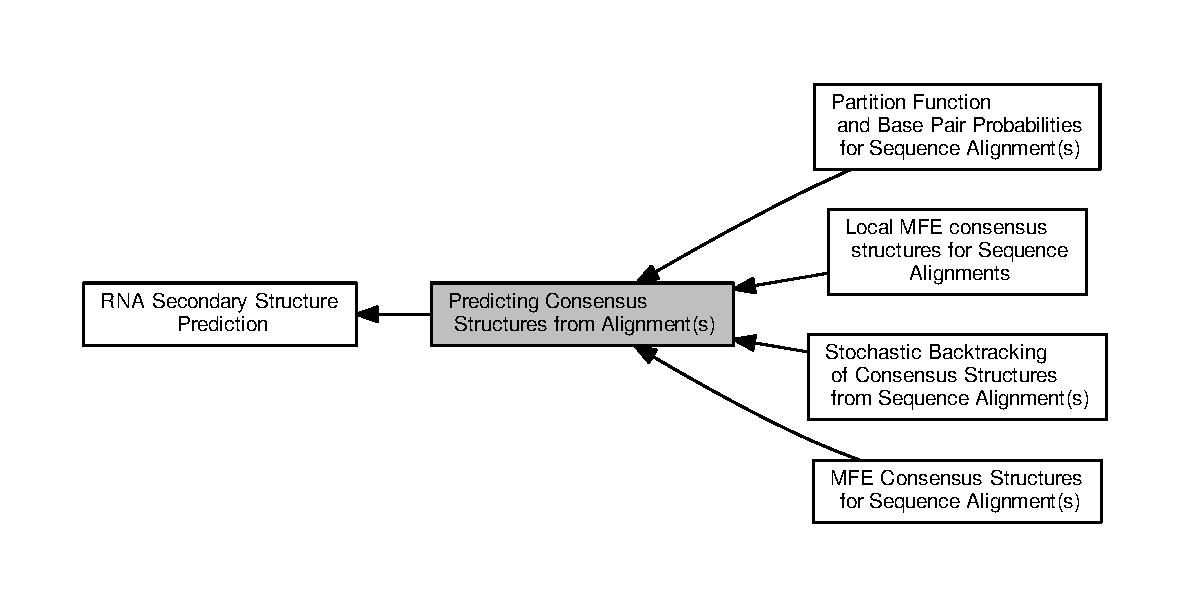
\includegraphics[width=350pt]{group__consensus__fold}
\end{center}
\end{figure}
\subsection*{Modules}
\begin{DoxyCompactItemize}
\item 
\hyperlink{group__consensus__mfe__fold}{M\+F\+E Consensus Structures for Sequence Alignment(s)}
\item 
\hyperlink{group__consensus__pf__fold}{Partition Function and Base Pair Probabilities for Sequence Alignment(s)}
\item 
\hyperlink{group__consensus__stochbt}{Stochastic Backtracking of Consensus Structures from Sequence Alignment(s)}
\item 
\hyperlink{group__local__consensus__fold}{Local M\+F\+E consensus structures for Sequence Alignments}
\end{DoxyCompactItemize}
\subsection*{Files}
\begin{DoxyCompactItemize}
\item 
file \hyperlink{alifold_8h}{alifold.\+h}
\begin{DoxyCompactList}\small\item\em compute various properties (consensus M\+F\+E structures, partition function, Boltzmann distributed stochastic samples, ...) for R\+N\+A sequence alignments \end{DoxyCompactList}\end{DoxyCompactItemize}
\subsection*{Functions}
\begin{DoxyCompactItemize}
\item 
float \hyperlink{group__consensus__fold_ga1c48869c03b49a342bf4cbdd61900081}{energy\+\_\+of\+\_\+alistruct} (const char $\ast$$\ast$sequences, const char $\ast$structure, int n\+\_\+seq, float $\ast$energy)
\begin{DoxyCompactList}\small\item\em Calculate the free energy of a consensus structure given a set of aligned sequences. \end{DoxyCompactList}\item 
int \hyperlink{group__consensus__fold_ga5349960075b1847720a2e9df021e2675}{get\+\_\+alipf\+\_\+arrays} (short $\ast$$\ast$$\ast$S\+\_\+p, short $\ast$$\ast$$\ast$S5\+\_\+p, short $\ast$$\ast$$\ast$S3\+\_\+p, unsigned short $\ast$$\ast$$\ast$a2s\+\_\+p, char $\ast$$\ast$$\ast$Ss\+\_\+p, \hyperlink{group__data__structures_ga31125aeace516926bf7f251f759b6126}{F\+L\+T\+\_\+\+O\+R\+\_\+\+D\+B\+L} $\ast$$\ast$qb\+\_\+p, \hyperlink{group__data__structures_ga31125aeace516926bf7f251f759b6126}{F\+L\+T\+\_\+\+O\+R\+\_\+\+D\+B\+L} $\ast$$\ast$qm\+\_\+p, \hyperlink{group__data__structures_ga31125aeace516926bf7f251f759b6126}{F\+L\+T\+\_\+\+O\+R\+\_\+\+D\+B\+L} $\ast$$\ast$q1k\+\_\+p, \hyperlink{group__data__structures_ga31125aeace516926bf7f251f759b6126}{F\+L\+T\+\_\+\+O\+R\+\_\+\+D\+B\+L} $\ast$$\ast$qln\+\_\+p, short $\ast$$\ast$pscore)
\begin{DoxyCompactList}\small\item\em Get pointers to (almost) all relavant arrays used in alifold\textquotesingle{}s partition function computation. \end{DoxyCompactList}\item 
void \hyperlink{group__consensus__fold_gac484c6bd429bafbd353b91044508d8e9}{update\+\_\+alifold\+\_\+params} (void)
\begin{DoxyCompactList}\small\item\em Update the energy parameters for alifold function. \end{DoxyCompactList}\item 
int \hyperlink{group__consensus__fold_ga20fd17bb27891009af7ce839f5386177}{vrna\+\_\+aln\+\_\+mpi} (char $\ast$Alseq\mbox{[}$\,$\mbox{]}, int n\+\_\+seq, int length, int $\ast$mini)
\begin{DoxyCompactList}\small\item\em Get the mean pairwise identity in steps from ?to?(ident) \end{DoxyCompactList}\item 
int \hyperlink{group__consensus__fold_gaa2d600be90844094ec145ea14a314d2f}{get\+\_\+mpi} (char $\ast$Alseq\mbox{[}$\,$\mbox{]}, int n\+\_\+seq, int length, int $\ast$mini)
\begin{DoxyCompactList}\small\item\em Get the mean pairwise identity in steps from ?to?(ident) \end{DoxyCompactList}\item 
void \hyperlink{group__consensus__fold_gaa3e40277c837d6f7603afe319884c786}{encode\+\_\+ali\+\_\+sequence} (const char $\ast$sequence, short $\ast$S, short $\ast$s5, short $\ast$s3, char $\ast$ss, unsigned short $\ast$as, int \hyperlink{group__model__details_gaf9202a1a09f5828dc731e2d9a10fa111}{circ})
\begin{DoxyCompactList}\small\item\em Get arrays with encoded sequence of the alignment. \end{DoxyCompactList}\item 
void \hyperlink{group__consensus__fold_ga8a560930f7f2582cc3967723a86cfdfa}{alloc\+\_\+sequence\+\_\+arrays} (const char $\ast$$\ast$sequences, short $\ast$$\ast$$\ast$S, short $\ast$$\ast$$\ast$S5, short $\ast$$\ast$$\ast$S3, unsigned short $\ast$$\ast$$\ast$a2s, char $\ast$$\ast$$\ast$Ss, int \hyperlink{group__model__details_gaf9202a1a09f5828dc731e2d9a10fa111}{circ})
\begin{DoxyCompactList}\small\item\em Allocate memory for sequence array used to deal with aligned sequences. \end{DoxyCompactList}\item 
void \hyperlink{group__consensus__fold_ga298a420a8c879202e2617b3f724fde38}{free\+\_\+sequence\+\_\+arrays} (unsigned int n\+\_\+seq, short $\ast$$\ast$$\ast$S, short $\ast$$\ast$$\ast$S5, short $\ast$$\ast$$\ast$S3, unsigned short $\ast$$\ast$$\ast$a2s, char $\ast$$\ast$$\ast$Ss)
\begin{DoxyCompactList}\small\item\em Free the memory of the sequence arrays used to deal with aligned sequences. \end{DoxyCompactList}\item 
\hypertarget{group__consensus__fold_ga1116aed4b2dab5252cd23946d47d52c3}{}float $\ast$$\ast$ \hyperlink{group__consensus__fold_ga1116aed4b2dab5252cd23946d47d52c3}{get\+\_\+ribosum} (const char $\ast$$\ast$Alseq, int n\+\_\+seq, int length)\label{group__consensus__fold_ga1116aed4b2dab5252cd23946d47d52c3}

\begin{DoxyCompactList}\small\item\em Retrieve a Ribo\+Sum Scoring Matrix for a given Alignment. \end{DoxyCompactList}\end{DoxyCompactItemize}
\subsection*{Variables}
\begin{DoxyCompactItemize}
\item 
double \hyperlink{group__consensus__fold_gaf3cbac6ff5d706d6e414677841ddf94c}{cv\+\_\+fact}
\begin{DoxyCompactList}\small\item\em This variable controls the weight of the covariance term in the energy function of alignment folding algorithms. \end{DoxyCompactList}\item 
double \hyperlink{group__consensus__fold_ga502948a122a2af5b914355b1f3ea2f61}{nc\+\_\+fact}
\begin{DoxyCompactList}\small\item\em This variable controls the magnitude of the penalty for non-\/compatible sequences in the covariance term of alignment folding algorithms. \end{DoxyCompactList}\end{DoxyCompactItemize}


\subsection{Detailed Description}
compute various properties (consensus M\+F\+E structures, partition function, Boltzmann distributed stochastic samples, ...) for R\+N\+A sequence alignments 

Consensus structures can be predicted by a modified version of the \hyperlink{group__mfe__fold__single_gaadafcb0f140795ae62e5ca027e335a9b}{fold()} algorithm that takes a set of aligned sequences instead of a single sequence. The energy function consists of the mean energy averaged over the sequences, plus a covariance term that favors pairs with consistent and compensatory mutations and penalizes pairs that cannot be formed by all structures. For details see \cite{hofacker:2002} and \cite{bernhart:2008}. 

\subsection{Function Documentation}
\hypertarget{group__consensus__fold_ga1c48869c03b49a342bf4cbdd61900081}{}\index{Predicting Consensus Structures from Alignment(s)@{Predicting Consensus Structures from Alignment(s)}!energy\+\_\+of\+\_\+alistruct@{energy\+\_\+of\+\_\+alistruct}}
\index{energy\+\_\+of\+\_\+alistruct@{energy\+\_\+of\+\_\+alistruct}!Predicting Consensus Structures from Alignment(s)@{Predicting Consensus Structures from Alignment(s)}}
\subsubsection[{energy\+\_\+of\+\_\+alistruct}]{\setlength{\rightskip}{0pt plus 5cm}float energy\+\_\+of\+\_\+alistruct (
\begin{DoxyParamCaption}
\item[{const char $\ast$$\ast$}]{sequences, }
\item[{const char $\ast$}]{structure, }
\item[{int}]{n\+\_\+seq, }
\item[{float $\ast$}]{energy}
\end{DoxyParamCaption}
)}\label{group__consensus__fold_ga1c48869c03b49a342bf4cbdd61900081}


{\ttfamily \#include $<$\hyperlink{alifold_8h}{Vienna\+R\+N\+A/alifold.\+h}$>$}



Calculate the free energy of a consensus structure given a set of aligned sequences. 

\begin{DoxyRefDesc}{Deprecated}
\item[\hyperlink{deprecated__deprecated000015}{Deprecated}]Usage of this function is discouraged! Use \hyperlink{group__eval_ga58f199f1438d794a265f3b27fc8ea631}{vrna\+\_\+eval\+\_\+structure()}, and \hyperlink{group__eval_ga6cea75c0eb9857fb59172be54cab09e0}{vrna\+\_\+eval\+\_\+covar\+\_\+structure()} instead!\end{DoxyRefDesc}



\begin{DoxyParams}{Parameters}
{\em sequences} & The N\+U\+L\+L terminated array of sequences \\
\hline
{\em structure} & The consensus structure \\
\hline
{\em n\+\_\+seq} & The number of sequences in the alignment \\
\hline
{\em energy} & A pointer to an array of at least two floats that will hold the free energies (energy\mbox{[}0\mbox{]} will contain the free energy, energy\mbox{[}1\mbox{]} will be filled with the covariance energy term) \\
\hline
\end{DoxyParams}
\begin{DoxyReturn}{Returns}
free energy in kcal/mol 
\end{DoxyReturn}
\hypertarget{group__consensus__fold_ga5349960075b1847720a2e9df021e2675}{}\index{Predicting Consensus Structures from Alignment(s)@{Predicting Consensus Structures from Alignment(s)}!get\+\_\+alipf\+\_\+arrays@{get\+\_\+alipf\+\_\+arrays}}
\index{get\+\_\+alipf\+\_\+arrays@{get\+\_\+alipf\+\_\+arrays}!Predicting Consensus Structures from Alignment(s)@{Predicting Consensus Structures from Alignment(s)}}
\subsubsection[{get\+\_\+alipf\+\_\+arrays}]{\setlength{\rightskip}{0pt plus 5cm}int get\+\_\+alipf\+\_\+arrays (
\begin{DoxyParamCaption}
\item[{short $\ast$$\ast$$\ast$}]{S\+\_\+p, }
\item[{short $\ast$$\ast$$\ast$}]{S5\+\_\+p, }
\item[{short $\ast$$\ast$$\ast$}]{S3\+\_\+p, }
\item[{unsigned short $\ast$$\ast$$\ast$}]{a2s\+\_\+p, }
\item[{char $\ast$$\ast$$\ast$}]{Ss\+\_\+p, }
\item[{{\bf F\+L\+T\+\_\+\+O\+R\+\_\+\+D\+B\+L} $\ast$$\ast$}]{qb\+\_\+p, }
\item[{{\bf F\+L\+T\+\_\+\+O\+R\+\_\+\+D\+B\+L} $\ast$$\ast$}]{qm\+\_\+p, }
\item[{{\bf F\+L\+T\+\_\+\+O\+R\+\_\+\+D\+B\+L} $\ast$$\ast$}]{q1k\+\_\+p, }
\item[{{\bf F\+L\+T\+\_\+\+O\+R\+\_\+\+D\+B\+L} $\ast$$\ast$}]{qln\+\_\+p, }
\item[{short $\ast$$\ast$}]{pscore}
\end{DoxyParamCaption}
)}\label{group__consensus__fold_ga5349960075b1847720a2e9df021e2675}


{\ttfamily \#include $<$\hyperlink{alifold_8h}{Vienna\+R\+N\+A/alifold.\+h}$>$}



Get pointers to (almost) all relavant arrays used in alifold\textquotesingle{}s partition function computation. 

\begin{DoxyNote}{Note}
To obtain meaningful pointers, call alipf\+\_\+fold first!
\end{DoxyNote}
\begin{DoxySeeAlso}{See also}
pf\+\_\+alifold(), \hyperlink{group__consensus__pf__fold_gaadd8d570442f86cbbc4978c8c62c9646}{alipf\+\_\+circ\+\_\+fold()}
\end{DoxySeeAlso}
\begin{DoxyRefDesc}{Deprecated}
\item[\hyperlink{deprecated__deprecated000024}{Deprecated}]It is discouraged to use this function! The new \hyperlink{group__fold__compound_ga1b0cef17fd40466cef5968eaeeff6166}{vrna\+\_\+fold\+\_\+compound\+\_\+t} allows direct access to all necessary consensus structure prediction related variables!\end{DoxyRefDesc}


\begin{DoxySeeAlso}{See also}
\hyperlink{group__fold__compound_ga1b0cef17fd40466cef5968eaeeff6166}{vrna\+\_\+fold\+\_\+compound\+\_\+t}, \hyperlink{group__fold__compound_gad6bacc816af274922b13d947f708aa0c}{vrna\+\_\+fold\+\_\+compound\+\_\+comparative()}, \hyperlink{group__pf__fold_ga29e256d688ad221b78d37f427e0e99bc}{vrna\+\_\+pf()}
\end{DoxySeeAlso}

\begin{DoxyParams}{Parameters}
{\em S\+\_\+p} & A pointer to the \textquotesingle{}S\textquotesingle{} array (integer representation of nucleotides) \\
\hline
{\em S5\+\_\+p} & A pointer to the \textquotesingle{}S5\textquotesingle{} array \\
\hline
{\em S3\+\_\+p} & A pointer to the \textquotesingle{}S3\textquotesingle{} array \\
\hline
{\em a2s\+\_\+p} & A pointer to the pair type matrix \\
\hline
{\em Ss\+\_\+p} & A pointer to the \textquotesingle{}Ss\textquotesingle{} array \\
\hline
{\em qb\+\_\+p} & A pointer to the Q\textsuperscript{B} matrix \\
\hline
{\em qm\+\_\+p} & A pointer to the Q\textsuperscript{M} matrix \\
\hline
{\em q1k\+\_\+p} & A pointer to the 5\textquotesingle{} slice of the Q matrix ( $q1k(k) = Q(1, k)$) \\
\hline
{\em qln\+\_\+p} & A pointer to the 3\textquotesingle{} slice of the Q matrix ( $qln(l) = Q(l, n)$) \\
\hline
\end{DoxyParams}
\begin{DoxyReturn}{Returns}
Non Zero if everything went fine, 0 otherwise 
\end{DoxyReturn}
\hypertarget{group__consensus__fold_gac484c6bd429bafbd353b91044508d8e9}{}\index{Predicting Consensus Structures from Alignment(s)@{Predicting Consensus Structures from Alignment(s)}!update\+\_\+alifold\+\_\+params@{update\+\_\+alifold\+\_\+params}}
\index{update\+\_\+alifold\+\_\+params@{update\+\_\+alifold\+\_\+params}!Predicting Consensus Structures from Alignment(s)@{Predicting Consensus Structures from Alignment(s)}}
\subsubsection[{update\+\_\+alifold\+\_\+params}]{\setlength{\rightskip}{0pt plus 5cm}void update\+\_\+alifold\+\_\+params (
\begin{DoxyParamCaption}
\item[{void}]{}
\end{DoxyParamCaption}
)}\label{group__consensus__fold_gac484c6bd429bafbd353b91044508d8e9}


{\ttfamily \#include $<$\hyperlink{alifold_8h}{Vienna\+R\+N\+A/alifold.\+h}$>$}



Update the energy parameters for alifold function. 

Call this to recalculate the pair matrix and energy parameters after a change in folding parameters like \hyperlink{group__model__details_gab4b11c8d9c758430960896bc3fe82ead}{temperature}

\begin{DoxyRefDesc}{Deprecated}
\item[\hyperlink{deprecated__deprecated000025}{Deprecated}]Usage of this function is discouraged! The new A\+P\+I uses \hyperlink{group__fold__compound_ga1b0cef17fd40466cef5968eaeeff6166}{vrna\+\_\+fold\+\_\+compound\+\_\+t} to lump all folding related necessities together, including the energy parameters. Use vrna\+\_\+update\+\_\+fold\+\_\+params() to update the energy parameters within a \hyperlink{group__fold__compound_ga1b0cef17fd40466cef5968eaeeff6166}{vrna\+\_\+fold\+\_\+compound\+\_\+t}. \end{DoxyRefDesc}
\hypertarget{group__consensus__fold_ga20fd17bb27891009af7ce839f5386177}{}\index{Predicting Consensus Structures from Alignment(s)@{Predicting Consensus Structures from Alignment(s)}!vrna\+\_\+aln\+\_\+mpi@{vrna\+\_\+aln\+\_\+mpi}}
\index{vrna\+\_\+aln\+\_\+mpi@{vrna\+\_\+aln\+\_\+mpi}!Predicting Consensus Structures from Alignment(s)@{Predicting Consensus Structures from Alignment(s)}}
\subsubsection[{vrna\+\_\+aln\+\_\+mpi}]{\setlength{\rightskip}{0pt plus 5cm}int vrna\+\_\+aln\+\_\+mpi (
\begin{DoxyParamCaption}
\item[{char $\ast$}]{Alseq\mbox{[}$\,$\mbox{]}, }
\item[{int}]{n\+\_\+seq, }
\item[{int}]{length, }
\item[{int $\ast$}]{mini}
\end{DoxyParamCaption}
)}\label{group__consensus__fold_ga20fd17bb27891009af7ce839f5386177}


{\ttfamily \#include $<$\hyperlink{aln__util_8h}{Vienna\+R\+N\+A/aln\+\_\+util.\+h}$>$}



Get the mean pairwise identity in steps from ?to?(ident) 


\begin{DoxyParams}{Parameters}
{\em Alseq} & \\
\hline
{\em n\+\_\+seq} & The number of sequences in the alignment \\
\hline
{\em length} & The length of the alignment \\
\hline
{\em mini} & \\
\hline
\end{DoxyParams}
\begin{DoxyReturn}{Returns}
The mean pairwise identity 
\end{DoxyReturn}
\hypertarget{group__consensus__fold_gaa2d600be90844094ec145ea14a314d2f}{}\index{Predicting Consensus Structures from Alignment(s)@{Predicting Consensus Structures from Alignment(s)}!get\+\_\+mpi@{get\+\_\+mpi}}
\index{get\+\_\+mpi@{get\+\_\+mpi}!Predicting Consensus Structures from Alignment(s)@{Predicting Consensus Structures from Alignment(s)}}
\subsubsection[{get\+\_\+mpi}]{\setlength{\rightskip}{0pt plus 5cm}int get\+\_\+mpi (
\begin{DoxyParamCaption}
\item[{char $\ast$}]{Alseq\mbox{[}$\,$\mbox{]}, }
\item[{int}]{n\+\_\+seq, }
\item[{int}]{length, }
\item[{int $\ast$}]{mini}
\end{DoxyParamCaption}
)}\label{group__consensus__fold_gaa2d600be90844094ec145ea14a314d2f}


{\ttfamily \#include $<$\hyperlink{aln__util_8h}{Vienna\+R\+N\+A/aln\+\_\+util.\+h}$>$}



Get the mean pairwise identity in steps from ?to?(ident) 

\begin{DoxyRefDesc}{Deprecated}
\item[\hyperlink{deprecated__deprecated000027}{Deprecated}]Use \hyperlink{group__consensus__fold_ga20fd17bb27891009af7ce839f5386177}{vrna\+\_\+aln\+\_\+mpi()} as a replacement\end{DoxyRefDesc}



\begin{DoxyParams}{Parameters}
{\em Alseq} & \\
\hline
{\em n\+\_\+seq} & The number of sequences in the alignment \\
\hline
{\em length} & The length of the alignment \\
\hline
{\em mini} & \\
\hline
\end{DoxyParams}
\begin{DoxyReturn}{Returns}
The mean pairwise identity 
\end{DoxyReturn}
\hypertarget{group__consensus__fold_gaa3e40277c837d6f7603afe319884c786}{}\index{Predicting Consensus Structures from Alignment(s)@{Predicting Consensus Structures from Alignment(s)}!encode\+\_\+ali\+\_\+sequence@{encode\+\_\+ali\+\_\+sequence}}
\index{encode\+\_\+ali\+\_\+sequence@{encode\+\_\+ali\+\_\+sequence}!Predicting Consensus Structures from Alignment(s)@{Predicting Consensus Structures from Alignment(s)}}
\subsubsection[{encode\+\_\+ali\+\_\+sequence}]{\setlength{\rightskip}{0pt plus 5cm}void encode\+\_\+ali\+\_\+sequence (
\begin{DoxyParamCaption}
\item[{const char $\ast$}]{sequence, }
\item[{short $\ast$}]{S, }
\item[{short $\ast$}]{s5, }
\item[{short $\ast$}]{s3, }
\item[{char $\ast$}]{ss, }
\item[{unsigned short $\ast$}]{as, }
\item[{int}]{circ}
\end{DoxyParamCaption}
)}\label{group__consensus__fold_gaa3e40277c837d6f7603afe319884c786}


{\ttfamily \#include $<$\hyperlink{aln__util_8h}{Vienna\+R\+N\+A/aln\+\_\+util.\+h}$>$}



Get arrays with encoded sequence of the alignment. 

this function assumes that in S, S5, s3, ss and as enough space is already allocated (size must be at least sequence length+2)


\begin{DoxyParams}{Parameters}
{\em sequence} & The gapped sequence from the alignment \\
\hline
{\em S} & pointer to an array that holds encoded sequence \\
\hline
{\em s5} & pointer to an array that holds the next base 5\textquotesingle{} of alignment position i \\
\hline
{\em s3} & pointer to an array that holds the next base 3\textquotesingle{} of alignment position i \\
\hline
{\em ss} & \\
\hline
{\em as} & \\
\hline
{\em circ} & assume the molecules to be circular instead of linear (circ=0) \\
\hline
\end{DoxyParams}
\hypertarget{group__consensus__fold_ga8a560930f7f2582cc3967723a86cfdfa}{}\index{Predicting Consensus Structures from Alignment(s)@{Predicting Consensus Structures from Alignment(s)}!alloc\+\_\+sequence\+\_\+arrays@{alloc\+\_\+sequence\+\_\+arrays}}
\index{alloc\+\_\+sequence\+\_\+arrays@{alloc\+\_\+sequence\+\_\+arrays}!Predicting Consensus Structures from Alignment(s)@{Predicting Consensus Structures from Alignment(s)}}
\subsubsection[{alloc\+\_\+sequence\+\_\+arrays}]{\setlength{\rightskip}{0pt plus 5cm}void alloc\+\_\+sequence\+\_\+arrays (
\begin{DoxyParamCaption}
\item[{const char $\ast$$\ast$}]{sequences, }
\item[{short $\ast$$\ast$$\ast$}]{S, }
\item[{short $\ast$$\ast$$\ast$}]{S5, }
\item[{short $\ast$$\ast$$\ast$}]{S3, }
\item[{unsigned short $\ast$$\ast$$\ast$}]{a2s, }
\item[{char $\ast$$\ast$$\ast$}]{Ss, }
\item[{int}]{circ}
\end{DoxyParamCaption}
)}\label{group__consensus__fold_ga8a560930f7f2582cc3967723a86cfdfa}


{\ttfamily \#include $<$\hyperlink{aln__util_8h}{Vienna\+R\+N\+A/aln\+\_\+util.\+h}$>$}



Allocate memory for sequence array used to deal with aligned sequences. 

Note that these arrays will also be initialized according to the sequence alignment given

\begin{DoxySeeAlso}{See also}
\hyperlink{group__consensus__fold_ga298a420a8c879202e2617b3f724fde38}{free\+\_\+sequence\+\_\+arrays()}
\end{DoxySeeAlso}

\begin{DoxyParams}{Parameters}
{\em sequences} & The aligned sequences \\
\hline
{\em S} & A pointer to the array of encoded sequences \\
\hline
{\em S5} & A pointer to the array that contains the next 5\textquotesingle{} nucleotide of a sequence position \\
\hline
{\em S3} & A pointer to the array that contains the next 3\textquotesingle{} nucleotide of a sequence position \\
\hline
{\em a2s} & A pointer to the array that contains the alignment to sequence position mapping \\
\hline
{\em Ss} & A pointer to the array that contains the ungapped sequence \\
\hline
{\em circ} & assume the molecules to be circular instead of linear (circ=0) \\
\hline
\end{DoxyParams}
\hypertarget{group__consensus__fold_ga298a420a8c879202e2617b3f724fde38}{}\index{Predicting Consensus Structures from Alignment(s)@{Predicting Consensus Structures from Alignment(s)}!free\+\_\+sequence\+\_\+arrays@{free\+\_\+sequence\+\_\+arrays}}
\index{free\+\_\+sequence\+\_\+arrays@{free\+\_\+sequence\+\_\+arrays}!Predicting Consensus Structures from Alignment(s)@{Predicting Consensus Structures from Alignment(s)}}
\subsubsection[{free\+\_\+sequence\+\_\+arrays}]{\setlength{\rightskip}{0pt plus 5cm}void free\+\_\+sequence\+\_\+arrays (
\begin{DoxyParamCaption}
\item[{unsigned int}]{n\+\_\+seq, }
\item[{short $\ast$$\ast$$\ast$}]{S, }
\item[{short $\ast$$\ast$$\ast$}]{S5, }
\item[{short $\ast$$\ast$$\ast$}]{S3, }
\item[{unsigned short $\ast$$\ast$$\ast$}]{a2s, }
\item[{char $\ast$$\ast$$\ast$}]{Ss}
\end{DoxyParamCaption}
)}\label{group__consensus__fold_ga298a420a8c879202e2617b3f724fde38}


{\ttfamily \#include $<$\hyperlink{aln__util_8h}{Vienna\+R\+N\+A/aln\+\_\+util.\+h}$>$}



Free the memory of the sequence arrays used to deal with aligned sequences. 

This function frees the memory previously allocated with \hyperlink{group__consensus__fold_ga8a560930f7f2582cc3967723a86cfdfa}{alloc\+\_\+sequence\+\_\+arrays()}

\begin{DoxySeeAlso}{See also}
\hyperlink{group__consensus__fold_ga8a560930f7f2582cc3967723a86cfdfa}{alloc\+\_\+sequence\+\_\+arrays()}
\end{DoxySeeAlso}

\begin{DoxyParams}{Parameters}
{\em n\+\_\+seq} & The number of aligned sequences \\
\hline
{\em S} & A pointer to the array of encoded sequences \\
\hline
{\em S5} & A pointer to the array that contains the next 5\textquotesingle{} nucleotide of a sequence position \\
\hline
{\em S3} & A pointer to the array that contains the next 3\textquotesingle{} nucleotide of a sequence position \\
\hline
{\em a2s} & A pointer to the array that contains the alignment to sequence position mapping \\
\hline
{\em Ss} & A pointer to the array that contains the ungapped sequence \\
\hline
\end{DoxyParams}


\subsection{Variable Documentation}
\hypertarget{group__consensus__fold_gaf3cbac6ff5d706d6e414677841ddf94c}{}\index{Predicting Consensus Structures from Alignment(s)@{Predicting Consensus Structures from Alignment(s)}!cv\+\_\+fact@{cv\+\_\+fact}}
\index{cv\+\_\+fact@{cv\+\_\+fact}!Predicting Consensus Structures from Alignment(s)@{Predicting Consensus Structures from Alignment(s)}}
\subsubsection[{cv\+\_\+fact}]{\setlength{\rightskip}{0pt plus 5cm}double cv\+\_\+fact}\label{group__consensus__fold_gaf3cbac6ff5d706d6e414677841ddf94c}


{\ttfamily \#include $<$\hyperlink{alifold_8h}{Vienna\+R\+N\+A/alifold.\+h}$>$}



This variable controls the weight of the covariance term in the energy function of alignment folding algorithms. 

\begin{DoxyRefDesc}{Deprecated}
\item[\hyperlink{deprecated__deprecated000016}{Deprecated}]See \hyperlink{group__model__details_a62ebefb9d0643e5c4c8a2ec84a105ce6}{vrna\+\_\+md\+\_\+t.\+cv\+\_\+fact}, and \hyperlink{group__mfe__fold_gabd3b147371ccf25c577f88bbbaf159fd}{vrna\+\_\+mfe()} to avoid using global variables\end{DoxyRefDesc}


Default is 1. \hypertarget{group__consensus__fold_ga502948a122a2af5b914355b1f3ea2f61}{}\index{Predicting Consensus Structures from Alignment(s)@{Predicting Consensus Structures from Alignment(s)}!nc\+\_\+fact@{nc\+\_\+fact}}
\index{nc\+\_\+fact@{nc\+\_\+fact}!Predicting Consensus Structures from Alignment(s)@{Predicting Consensus Structures from Alignment(s)}}
\subsubsection[{nc\+\_\+fact}]{\setlength{\rightskip}{0pt plus 5cm}double nc\+\_\+fact}\label{group__consensus__fold_ga502948a122a2af5b914355b1f3ea2f61}


{\ttfamily \#include $<$\hyperlink{alifold_8h}{Vienna\+R\+N\+A/alifold.\+h}$>$}



This variable controls the magnitude of the penalty for non-\/compatible sequences in the covariance term of alignment folding algorithms. 

\begin{DoxyRefDesc}{Deprecated}
\item[\hyperlink{deprecated__deprecated000017}{Deprecated}]See \#vrna\+\_\+md\+\_\+t.\+nc\+\_\+fact, and \hyperlink{group__mfe__fold_gabd3b147371ccf25c577f88bbbaf159fd}{vrna\+\_\+mfe()} to avoid using global variables\end{DoxyRefDesc}


Default is 1. 
\hypertarget{group__consensus__mfe__fold}{}\section{M\+F\+E Consensus Structures for Sequence Alignment(s)}
\label{group__consensus__mfe__fold}\index{M\+F\+E Consensus Structures for Sequence Alignment(s)@{M\+F\+E Consensus Structures for Sequence Alignment(s)}}
Collaboration diagram for M\+F\+E Consensus Structures for Sequence Alignment(s)\+:
\nopagebreak
\begin{figure}[H]
\begin{center}
\leavevmode
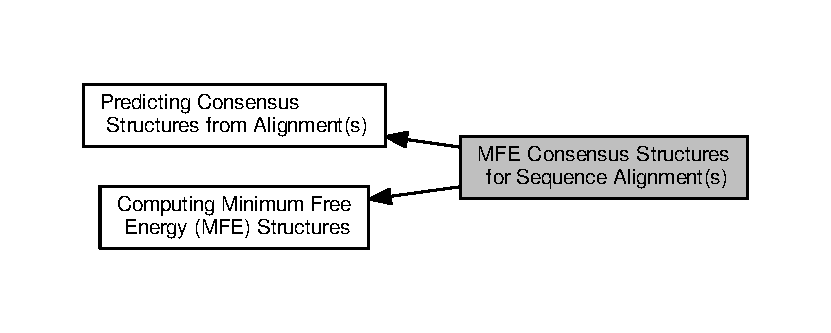
\includegraphics[width=350pt]{group__consensus__mfe__fold}
\end{center}
\end{figure}
\subsection*{Functions}
\begin{DoxyCompactItemize}
\item 
float \hyperlink{group__consensus__mfe__fold_ga02098d0c8790f9a37fbef6ad0cfc705c}{vrna\+\_\+alifold} (const char $\ast$$\ast$ssequences, char $\ast$structure)
\begin{DoxyCompactList}\small\item\em Compute Minimum Free Energy (M\+F\+E), and a corresponding consensus secondary structure for an R\+N\+A sequence alignment using a comparative method. \end{DoxyCompactList}\item 
float \hyperlink{group__consensus__mfe__fold_ga01ce2cff93ea44c4f4254760ca2bd16c}{vrna\+\_\+circalifold} (const char $\ast$$\ast$ssequences, char $\ast$structure)
\begin{DoxyCompactList}\small\item\em Compute Minimum Free Energy (M\+F\+E), and a corresponding consensus secondary structure for a sequence alignment of circular R\+N\+As using a comparative method. \end{DoxyCompactList}\item 
float \hyperlink{group__consensus__mfe__fold_ga4cf00f0659e5f0480335d69e797f05b1}{alifold} (const char $\ast$$\ast$strings, char $\ast$structure)
\begin{DoxyCompactList}\small\item\em Compute M\+F\+E and according consensus structure of an alignment of sequences. \end{DoxyCompactList}\item 
float \hyperlink{group__consensus__mfe__fold_gadbd3b0b1c144cbfb4efe704b2b260f96}{circalifold} (const char $\ast$$\ast$strings, char $\ast$structure)
\begin{DoxyCompactList}\small\item\em Compute M\+F\+E and according structure of an alignment of sequences assuming the sequences are circular instead of linear. \end{DoxyCompactList}\item 
void \hyperlink{group__consensus__mfe__fold_ga72095e4554b5d577250ea14c42acc49e}{free\+\_\+alifold\+\_\+arrays} (void)
\begin{DoxyCompactList}\small\item\em Free the memory occupied by M\+F\+E alifold functions. \end{DoxyCompactList}\end{DoxyCompactItemize}


\subsection{Detailed Description}


\subsection{Function Documentation}
\hypertarget{group__consensus__mfe__fold_ga02098d0c8790f9a37fbef6ad0cfc705c}{}\index{M\+F\+E Consensus Structures for Sequence Alignment(s)@{M\+F\+E Consensus Structures for Sequence Alignment(s)}!vrna\+\_\+alifold@{vrna\+\_\+alifold}}
\index{vrna\+\_\+alifold@{vrna\+\_\+alifold}!M\+F\+E Consensus Structures for Sequence Alignment(s)@{M\+F\+E Consensus Structures for Sequence Alignment(s)}}
\subsubsection[{vrna\+\_\+alifold}]{\setlength{\rightskip}{0pt plus 5cm}float vrna\+\_\+alifold (
\begin{DoxyParamCaption}
\item[{const char $\ast$$\ast$}]{ssequences, }
\item[{char $\ast$}]{structure}
\end{DoxyParamCaption}
)}\label{group__consensus__mfe__fold_ga02098d0c8790f9a37fbef6ad0cfc705c}


{\ttfamily \#include $<$\hyperlink{alifold_8h}{Vienna\+R\+N\+A/alifold.\+h}$>$}



Compute Minimum Free Energy (M\+F\+E), and a corresponding consensus secondary structure for an R\+N\+A sequence alignment using a comparative method. 

This simplified interface to \hyperlink{group__mfe__fold_gabd3b147371ccf25c577f88bbbaf159fd}{vrna\+\_\+mfe()} computes the M\+F\+E and, if required, a consensus secondary structure for an R\+N\+A sequence alignment using default options. Memory required for dynamic programming (D\+P) matrices will be allocated and free\textquotesingle{}d on-\/the-\/fly. Hence, after return of this function, the recursively filled matrices are not available any more for any post-\/processing, e.\+g. suboptimal backtracking, etc.

\begin{DoxyNote}{Note}
In case you want to use the filled D\+P matrices for any subsequent post-\/processing step, or you require other conditions than specified by the default model details, use \hyperlink{group__mfe__fold_gabd3b147371ccf25c577f88bbbaf159fd}{vrna\+\_\+mfe()}, and the data structure \hyperlink{group__fold__compound_ga1b0cef17fd40466cef5968eaeeff6166}{vrna\+\_\+fold\+\_\+compound\+\_\+t} instead.
\end{DoxyNote}
\begin{DoxySeeAlso}{See also}
\hyperlink{group__consensus__mfe__fold_ga01ce2cff93ea44c4f4254760ca2bd16c}{vrna\+\_\+circalifold()}, \hyperlink{group__mfe__fold_gabd3b147371ccf25c577f88bbbaf159fd}{vrna\+\_\+mfe()}, \hyperlink{group__fold__compound_ga6601d994ba32b11511b36f68b08403be}{vrna\+\_\+fold\+\_\+compound()}, \hyperlink{group__fold__compound_ga1b0cef17fd40466cef5968eaeeff6166}{vrna\+\_\+fold\+\_\+compound\+\_\+t}
\end{DoxySeeAlso}

\begin{DoxyParams}{Parameters}
{\em sequences} & R\+N\+A sequence alignment \\
\hline
{\em structure} & A pointer to the character array where the secondary structure in dot-\/bracket notation will be written to \\
\hline
\end{DoxyParams}
\begin{DoxyReturn}{Returns}
the minimum free energy (M\+F\+E) in kcal/mol 
\end{DoxyReturn}
\hypertarget{group__consensus__mfe__fold_ga01ce2cff93ea44c4f4254760ca2bd16c}{}\index{M\+F\+E Consensus Structures for Sequence Alignment(s)@{M\+F\+E Consensus Structures for Sequence Alignment(s)}!vrna\+\_\+circalifold@{vrna\+\_\+circalifold}}
\index{vrna\+\_\+circalifold@{vrna\+\_\+circalifold}!M\+F\+E Consensus Structures for Sequence Alignment(s)@{M\+F\+E Consensus Structures for Sequence Alignment(s)}}
\subsubsection[{vrna\+\_\+circalifold}]{\setlength{\rightskip}{0pt plus 5cm}float vrna\+\_\+circalifold (
\begin{DoxyParamCaption}
\item[{const char $\ast$$\ast$}]{ssequences, }
\item[{char $\ast$}]{structure}
\end{DoxyParamCaption}
)}\label{group__consensus__mfe__fold_ga01ce2cff93ea44c4f4254760ca2bd16c}


{\ttfamily \#include $<$\hyperlink{alifold_8h}{Vienna\+R\+N\+A/alifold.\+h}$>$}



Compute Minimum Free Energy (M\+F\+E), and a corresponding consensus secondary structure for a sequence alignment of circular R\+N\+As using a comparative method. 

This simplified interface to \hyperlink{group__mfe__fold_gabd3b147371ccf25c577f88bbbaf159fd}{vrna\+\_\+mfe()} computes the M\+F\+E and, if required, a consensus secondary structure for an R\+N\+A sequence alignment using default options. Memory required for dynamic programming (D\+P) matrices will be allocated and free\textquotesingle{}d on-\/the-\/fly. Hence, after return of this function, the recursively filled matrices are not available any more for any post-\/processing, e.\+g. suboptimal backtracking, etc.

Folding of circular R\+N\+A sequences is handled as a post-\/processing step of the forward recursions. See \cite{hofacker:2006} for further details.

\begin{DoxyNote}{Note}
In case you want to use the filled D\+P matrices for any subsequent post-\/processing step, or you require other conditions than specified by the default model details, use \hyperlink{group__mfe__fold_gabd3b147371ccf25c577f88bbbaf159fd}{vrna\+\_\+mfe()}, and the data structure \hyperlink{group__fold__compound_ga1b0cef17fd40466cef5968eaeeff6166}{vrna\+\_\+fold\+\_\+compound\+\_\+t} instead.
\end{DoxyNote}
\begin{DoxySeeAlso}{See also}
\hyperlink{group__consensus__mfe__fold_ga02098d0c8790f9a37fbef6ad0cfc705c}{vrna\+\_\+alifold()}, \hyperlink{group__mfe__fold_gabd3b147371ccf25c577f88bbbaf159fd}{vrna\+\_\+mfe()}, \hyperlink{group__fold__compound_ga6601d994ba32b11511b36f68b08403be}{vrna\+\_\+fold\+\_\+compound()}, \hyperlink{group__fold__compound_ga1b0cef17fd40466cef5968eaeeff6166}{vrna\+\_\+fold\+\_\+compound\+\_\+t}
\end{DoxySeeAlso}

\begin{DoxyParams}{Parameters}
{\em sequences} & Sequence alignment of circular R\+N\+As \\
\hline
{\em structure} & A pointer to the character array where the secondary structure in dot-\/bracket notation will be written to \\
\hline
\end{DoxyParams}
\begin{DoxyReturn}{Returns}
the minimum free energy (M\+F\+E) in kcal/mol 
\end{DoxyReturn}
\hypertarget{group__consensus__mfe__fold_ga4cf00f0659e5f0480335d69e797f05b1}{}\index{M\+F\+E Consensus Structures for Sequence Alignment(s)@{M\+F\+E Consensus Structures for Sequence Alignment(s)}!alifold@{alifold}}
\index{alifold@{alifold}!M\+F\+E Consensus Structures for Sequence Alignment(s)@{M\+F\+E Consensus Structures for Sequence Alignment(s)}}
\subsubsection[{alifold}]{\setlength{\rightskip}{0pt plus 5cm}float alifold (
\begin{DoxyParamCaption}
\item[{const char $\ast$$\ast$}]{strings, }
\item[{char $\ast$}]{structure}
\end{DoxyParamCaption}
)}\label{group__consensus__mfe__fold_ga4cf00f0659e5f0480335d69e797f05b1}


{\ttfamily \#include $<$\hyperlink{alifold_8h}{Vienna\+R\+N\+A/alifold.\+h}$>$}



Compute M\+F\+E and according consensus structure of an alignment of sequences. 

This function predicts the consensus structure for the aligned \textquotesingle{}sequences\textquotesingle{} and returns the minimum free energy; the mfe structure in bracket notation is returned in \textquotesingle{}structure\textquotesingle{}.

Sufficient space must be allocated for \textquotesingle{}structure\textquotesingle{} before calling \hyperlink{group__consensus__mfe__fold_ga4cf00f0659e5f0480335d69e797f05b1}{alifold()}.

\begin{DoxyRefDesc}{Deprecated}
\item[\hyperlink{deprecated__deprecated000012}{Deprecated}]Usage of this function is discouraged! Use \hyperlink{group__consensus__mfe__fold_ga02098d0c8790f9a37fbef6ad0cfc705c}{vrna\+\_\+alifold()}, or \hyperlink{group__mfe__fold_gabd3b147371ccf25c577f88bbbaf159fd}{vrna\+\_\+mfe()} instead! \begin{DoxySeeAlso}{See also}
\hyperlink{group__consensus__mfe__fold_ga02098d0c8790f9a37fbef6ad0cfc705c}{vrna\+\_\+alifold()}, \hyperlink{group__mfe__fold_gabd3b147371ccf25c577f88bbbaf159fd}{vrna\+\_\+mfe()}
\end{DoxySeeAlso}
\end{DoxyRefDesc}



\begin{DoxyParams}{Parameters}
{\em strings} & A pointer to a N\+U\+L\+L terminated array of character arrays \\
\hline
{\em structure} & A pointer to a character array that may contain a constraining consensus structure (will be overwritten by a consensus structure that exhibits the M\+F\+E) \\
\hline
\end{DoxyParams}
\begin{DoxyReturn}{Returns}
The free energy score in kcal/mol 
\end{DoxyReturn}
\hypertarget{group__consensus__mfe__fold_gadbd3b0b1c144cbfb4efe704b2b260f96}{}\index{M\+F\+E Consensus Structures for Sequence Alignment(s)@{M\+F\+E Consensus Structures for Sequence Alignment(s)}!circalifold@{circalifold}}
\index{circalifold@{circalifold}!M\+F\+E Consensus Structures for Sequence Alignment(s)@{M\+F\+E Consensus Structures for Sequence Alignment(s)}}
\subsubsection[{circalifold}]{\setlength{\rightskip}{0pt plus 5cm}float circalifold (
\begin{DoxyParamCaption}
\item[{const char $\ast$$\ast$}]{strings, }
\item[{char $\ast$}]{structure}
\end{DoxyParamCaption}
)}\label{group__consensus__mfe__fold_gadbd3b0b1c144cbfb4efe704b2b260f96}


{\ttfamily \#include $<$\hyperlink{alifold_8h}{Vienna\+R\+N\+A/alifold.\+h}$>$}



Compute M\+F\+E and according structure of an alignment of sequences assuming the sequences are circular instead of linear. 

\begin{DoxyRefDesc}{Deprecated}
\item[\hyperlink{deprecated__deprecated000013}{Deprecated}]Usage of this function is discouraged! Use vrna\+\_\+alicircfold(), and \hyperlink{group__mfe__fold_gabd3b147371ccf25c577f88bbbaf159fd}{vrna\+\_\+mfe()} instead! \begin{DoxySeeAlso}{See also}
vrna\+\_\+alicircfold(), \hyperlink{group__consensus__mfe__fold_ga02098d0c8790f9a37fbef6ad0cfc705c}{vrna\+\_\+alifold()}, \hyperlink{group__mfe__fold_gabd3b147371ccf25c577f88bbbaf159fd}{vrna\+\_\+mfe()}
\end{DoxySeeAlso}
\end{DoxyRefDesc}



\begin{DoxyParams}{Parameters}
{\em strings} & A pointer to a N\+U\+L\+L terminated array of character arrays \\
\hline
{\em structure} & A pointer to a character array that may contain a constraining consensus structure (will be overwritten by a consensus structure that exhibits the M\+F\+E) \\
\hline
\end{DoxyParams}
\begin{DoxyReturn}{Returns}
The free energy score in kcal/mol 
\end{DoxyReturn}
\hypertarget{group__consensus__mfe__fold_ga72095e4554b5d577250ea14c42acc49e}{}\index{M\+F\+E Consensus Structures for Sequence Alignment(s)@{M\+F\+E Consensus Structures for Sequence Alignment(s)}!free\+\_\+alifold\+\_\+arrays@{free\+\_\+alifold\+\_\+arrays}}
\index{free\+\_\+alifold\+\_\+arrays@{free\+\_\+alifold\+\_\+arrays}!M\+F\+E Consensus Structures for Sequence Alignment(s)@{M\+F\+E Consensus Structures for Sequence Alignment(s)}}
\subsubsection[{free\+\_\+alifold\+\_\+arrays}]{\setlength{\rightskip}{0pt plus 5cm}void free\+\_\+alifold\+\_\+arrays (
\begin{DoxyParamCaption}
\item[{void}]{}
\end{DoxyParamCaption}
)}\label{group__consensus__mfe__fold_ga72095e4554b5d577250ea14c42acc49e}


{\ttfamily \#include $<$\hyperlink{alifold_8h}{Vienna\+R\+N\+A/alifold.\+h}$>$}



Free the memory occupied by M\+F\+E alifold functions. 

\begin{DoxyRefDesc}{Deprecated}
\item[\hyperlink{deprecated__deprecated000014}{Deprecated}]Usage of this function is discouraged! It only affects memory being free\textquotesingle{}d that was allocated by an old A\+P\+I function before. Release of memory occupied by the newly introduced \hyperlink{group__fold__compound_ga1b0cef17fd40466cef5968eaeeff6166}{vrna\+\_\+fold\+\_\+compound\+\_\+t} is handled by vrna\+\_\+vrna\+\_\+fold\+\_\+compound\+\_\+free()\end{DoxyRefDesc}


\begin{DoxySeeAlso}{See also}
vrna\+\_\+vrna\+\_\+fold\+\_\+compound\+\_\+free() 
\end{DoxySeeAlso}

\hypertarget{group__consensus__pf__fold}{}\section{Partition Function and Base Pair Probabilities for Sequence Alignment(s)}
\label{group__consensus__pf__fold}\index{Partition Function and Base Pair Probabilities for Sequence Alignment(s)@{Partition Function and Base Pair Probabilities for Sequence Alignment(s)}}
Collaboration diagram for Partition Function and Base Pair Probabilities for Sequence Alignment(s)\+:
\nopagebreak
\begin{figure}[H]
\begin{center}
\leavevmode
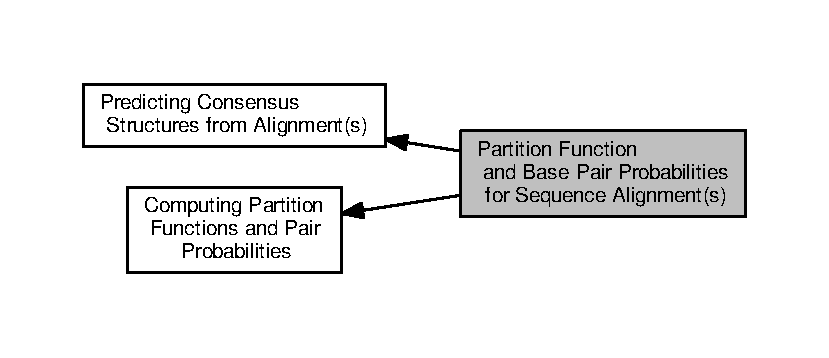
\includegraphics[width=350pt]{group__consensus__pf__fold}
\end{center}
\end{figure}
\subsection*{Functions}
\begin{DoxyCompactItemize}
\item 
float \hyperlink{group__consensus__pf__fold_gaef750636c70e597a85ee139197a4350d}{vrna\+\_\+pf\+\_\+alifold} (const char $\ast$$\ast$strings, char $\ast$structure, \hyperlink{group__data__structures_ga8e4eb5e1bfc95776559575beb359af87}{vrna\+\_\+plist\+\_\+t} $\ast$$\ast$pl)
\begin{DoxyCompactList}\small\item\em Compute Partition function $Q$ (and base pair probabilities) for an R\+N\+A sequence alignment using a comparative method. \end{DoxyCompactList}\item 
float \hyperlink{group__consensus__pf__fold_ga017209394a4c1e68d96cd47e61d16d25}{vrna\+\_\+pf\+\_\+circalifold} (const char $\ast$$\ast$sequences, char $\ast$structure, \hyperlink{group__data__structures_ga8e4eb5e1bfc95776559575beb359af87}{vrna\+\_\+plist\+\_\+t} $\ast$$\ast$pl)
\begin{DoxyCompactList}\small\item\em Compute Partition function $Q$ (and base pair probabilities) for an alignment of circular R\+N\+A sequences using a comparative method. \end{DoxyCompactList}\item 
float \hyperlink{group__consensus__pf__fold_ga5e8d54e41bf3d5b6e535d5bdb33c416e}{alipf\+\_\+fold\+\_\+par} (const char $\ast$$\ast$sequences, char $\ast$structure, \hyperlink{group__data__structures_ga8e4eb5e1bfc95776559575beb359af87}{vrna\+\_\+plist\+\_\+t} $\ast$$\ast$pl, \hyperlink{group__energy__parameters_ga01d8b92fe734df8d79a6169482c7d8d8}{vrna\+\_\+exp\+\_\+param\+\_\+t} $\ast$parameters, int calculate\+\_\+bppm, int is\+\_\+constrained, int is\+\_\+circular)
\item 
float \hyperlink{group__consensus__pf__fold_gaa150d3ba7b009a1c27cb6f0eb197f6b4}{alipf\+\_\+fold} (const char $\ast$$\ast$sequences, char $\ast$structure, \hyperlink{group__data__structures_ga8e4eb5e1bfc95776559575beb359af87}{vrna\+\_\+plist\+\_\+t} $\ast$$\ast$pl)
\begin{DoxyCompactList}\small\item\em The partition function version of \hyperlink{group__consensus__mfe__fold_ga4cf00f0659e5f0480335d69e797f05b1}{alifold()} works in analogy to \hyperlink{group__pf__fold_gadc3db3d98742427e7001a7fd36ef28c2}{pf\+\_\+fold()}. Pair probabilities and information about sequence covariations are returned via the \textquotesingle{}pi\textquotesingle{} variable as a list of \hyperlink{group__aln__utils_ga6660dfca23debee7306e0cd53341263f}{vrna\+\_\+pinfo\+\_\+t} structs. The list is terminated by the first entry with pi.\+i = 0. \end{DoxyCompactList}\item 
float \hyperlink{group__consensus__pf__fold_gaadd8d570442f86cbbc4978c8c62c9646}{alipf\+\_\+circ\+\_\+fold} (const char $\ast$$\ast$sequences, char $\ast$structure, \hyperlink{group__data__structures_ga8e4eb5e1bfc95776559575beb359af87}{vrna\+\_\+plist\+\_\+t} $\ast$$\ast$pl)
\item 
\hyperlink{group__data__structures_ga31125aeace516926bf7f251f759b6126}{F\+L\+T\+\_\+\+O\+R\+\_\+\+D\+B\+L} $\ast$ \hyperlink{group__consensus__pf__fold_ga11b6ab8bd9be1821fea352b190a01cab}{export\+\_\+ali\+\_\+bppm} (void)
\begin{DoxyCompactList}\small\item\em Get a pointer to the base pair probability array. \end{DoxyCompactList}\item 
void \hyperlink{group__consensus__pf__fold_ga0c0498f35686e26b38ee460d3db1a661}{free\+\_\+alipf\+\_\+arrays} (void)
\begin{DoxyCompactList}\small\item\em Free the memory occupied by folding matrices allocated by alipf\+\_\+fold, alipf\+\_\+circ\+\_\+fold, etc. \end{DoxyCompactList}\end{DoxyCompactItemize}


\subsection{Detailed Description}


\subsection{Function Documentation}
\hypertarget{group__consensus__pf__fold_gaef750636c70e597a85ee139197a4350d}{}\index{Partition Function and Base Pair Probabilities for Sequence Alignment(s)@{Partition Function and Base Pair Probabilities for Sequence Alignment(s)}!vrna\+\_\+pf\+\_\+alifold@{vrna\+\_\+pf\+\_\+alifold}}
\index{vrna\+\_\+pf\+\_\+alifold@{vrna\+\_\+pf\+\_\+alifold}!Partition Function and Base Pair Probabilities for Sequence Alignment(s)@{Partition Function and Base Pair Probabilities for Sequence Alignment(s)}}
\subsubsection[{vrna\+\_\+pf\+\_\+alifold}]{\setlength{\rightskip}{0pt plus 5cm}float vrna\+\_\+pf\+\_\+alifold (
\begin{DoxyParamCaption}
\item[{const char $\ast$$\ast$}]{strings, }
\item[{char $\ast$}]{structure, }
\item[{{\bf vrna\+\_\+plist\+\_\+t} $\ast$$\ast$}]{pl}
\end{DoxyParamCaption}
)}\label{group__consensus__pf__fold_gaef750636c70e597a85ee139197a4350d}


{\ttfamily \#include $<$\hyperlink{alifold_8h}{Vienna\+R\+N\+A/alifold.\+h}$>$}



Compute Partition function $Q$ (and base pair probabilities) for an R\+N\+A sequence alignment using a comparative method. 

This simplified interface to \hyperlink{group__pf__fold_ga29e256d688ad221b78d37f427e0e99bc}{vrna\+\_\+pf()} computes the partition function and, if required, base pair probabilities for an R\+N\+A sequence alignment using default options. Memory required for dynamic programming (D\+P) matrices will be allocated and free\textquotesingle{}d on-\/the-\/fly. Hence, after return of this function, the recursively filled matrices are not available any more for any post-\/processing.

\begin{DoxyNote}{Note}
In case you want to use the filled D\+P matrices for any subsequent post-\/processing step, or you require other conditions than specified by the default model details, use \hyperlink{group__pf__fold_ga29e256d688ad221b78d37f427e0e99bc}{vrna\+\_\+pf()}, and the data structure \hyperlink{group__fold__compound_ga1b0cef17fd40466cef5968eaeeff6166}{vrna\+\_\+fold\+\_\+compound\+\_\+t} instead.
\end{DoxyNote}
\begin{DoxySeeAlso}{See also}
\hyperlink{group__consensus__pf__fold_ga017209394a4c1e68d96cd47e61d16d25}{vrna\+\_\+pf\+\_\+circalifold()}, \hyperlink{group__pf__fold_ga29e256d688ad221b78d37f427e0e99bc}{vrna\+\_\+pf()}, \hyperlink{group__fold__compound_gad6bacc816af274922b13d947f708aa0c}{vrna\+\_\+fold\+\_\+compound\+\_\+comparative()}, \hyperlink{group__fold__compound_ga1b0cef17fd40466cef5968eaeeff6166}{vrna\+\_\+fold\+\_\+compound\+\_\+t}
\end{DoxySeeAlso}

\begin{DoxyParams}{Parameters}
{\em sequences} & R\+N\+A sequence alignment \\
\hline
{\em structure} & A pointer to the character array where position-\/wise pairing propensity will be stored. (Maybe N\+U\+L\+L) \\
\hline
{\em pl} & A pointer to a list of \hyperlink{group__data__structures_ga8e4eb5e1bfc95776559575beb359af87}{vrna\+\_\+plist\+\_\+t} to store pairing probabilities (Maybe N\+U\+L\+L) \\
\hline
\end{DoxyParams}
\begin{DoxyReturn}{Returns}
The Gibbs free energy of the ensemble ( $G = -RT \cdot \log(Q) $) in kcal/mol 
\end{DoxyReturn}
\hypertarget{group__consensus__pf__fold_ga017209394a4c1e68d96cd47e61d16d25}{}\index{Partition Function and Base Pair Probabilities for Sequence Alignment(s)@{Partition Function and Base Pair Probabilities for Sequence Alignment(s)}!vrna\+\_\+pf\+\_\+circalifold@{vrna\+\_\+pf\+\_\+circalifold}}
\index{vrna\+\_\+pf\+\_\+circalifold@{vrna\+\_\+pf\+\_\+circalifold}!Partition Function and Base Pair Probabilities for Sequence Alignment(s)@{Partition Function and Base Pair Probabilities for Sequence Alignment(s)}}
\subsubsection[{vrna\+\_\+pf\+\_\+circalifold}]{\setlength{\rightskip}{0pt plus 5cm}float vrna\+\_\+pf\+\_\+circalifold (
\begin{DoxyParamCaption}
\item[{const char $\ast$$\ast$}]{sequences, }
\item[{char $\ast$}]{structure, }
\item[{{\bf vrna\+\_\+plist\+\_\+t} $\ast$$\ast$}]{pl}
\end{DoxyParamCaption}
)}\label{group__consensus__pf__fold_ga017209394a4c1e68d96cd47e61d16d25}


{\ttfamily \#include $<$\hyperlink{alifold_8h}{Vienna\+R\+N\+A/alifold.\+h}$>$}



Compute Partition function $Q$ (and base pair probabilities) for an alignment of circular R\+N\+A sequences using a comparative method. 

This simplified interface to \hyperlink{group__pf__fold_ga29e256d688ad221b78d37f427e0e99bc}{vrna\+\_\+pf()} computes the partition function and, if required, base pair probabilities for an R\+N\+A sequence alignment using default options. Memory required for dynamic programming (D\+P) matrices will be allocated and free\textquotesingle{}d on-\/the-\/fly. Hence, after return of this function, the recursively filled matrices are not available any more for any post-\/processing.

\begin{DoxyNote}{Note}
In case you want to use the filled D\+P matrices for any subsequent post-\/processing step, or you require other conditions than specified by the default model details, use \hyperlink{group__pf__fold_ga29e256d688ad221b78d37f427e0e99bc}{vrna\+\_\+pf()}, and the data structure \hyperlink{group__fold__compound_ga1b0cef17fd40466cef5968eaeeff6166}{vrna\+\_\+fold\+\_\+compound\+\_\+t} instead.
\end{DoxyNote}
Folding of circular R\+N\+A sequences is handled as a post-\/processing step of the forward recursions. See \cite{hofacker:2006} for further details.

\begin{DoxySeeAlso}{See also}
\hyperlink{group__consensus__pf__fold_gaef750636c70e597a85ee139197a4350d}{vrna\+\_\+pf\+\_\+alifold()}, \hyperlink{group__pf__fold_ga29e256d688ad221b78d37f427e0e99bc}{vrna\+\_\+pf()}, \hyperlink{group__fold__compound_gad6bacc816af274922b13d947f708aa0c}{vrna\+\_\+fold\+\_\+compound\+\_\+comparative()}, \hyperlink{group__fold__compound_ga1b0cef17fd40466cef5968eaeeff6166}{vrna\+\_\+fold\+\_\+compound\+\_\+t}
\end{DoxySeeAlso}

\begin{DoxyParams}{Parameters}
{\em sequences} & Sequence alignment of circular R\+N\+As \\
\hline
{\em structure} & A pointer to the character array where position-\/wise pairing propensity will be stored. (Maybe N\+U\+L\+L) \\
\hline
{\em pl} & A pointer to a list of \hyperlink{group__data__structures_ga8e4eb5e1bfc95776559575beb359af87}{vrna\+\_\+plist\+\_\+t} to store pairing probabilities (Maybe N\+U\+L\+L) \\
\hline
\end{DoxyParams}
\begin{DoxyReturn}{Returns}
The Gibbs free energy of the ensemble ( $G = -RT \cdot \log(Q) $) in kcal/mol 
\end{DoxyReturn}
\hypertarget{group__consensus__pf__fold_ga5e8d54e41bf3d5b6e535d5bdb33c416e}{}\index{Partition Function and Base Pair Probabilities for Sequence Alignment(s)@{Partition Function and Base Pair Probabilities for Sequence Alignment(s)}!alipf\+\_\+fold\+\_\+par@{alipf\+\_\+fold\+\_\+par}}
\index{alipf\+\_\+fold\+\_\+par@{alipf\+\_\+fold\+\_\+par}!Partition Function and Base Pair Probabilities for Sequence Alignment(s)@{Partition Function and Base Pair Probabilities for Sequence Alignment(s)}}
\subsubsection[{alipf\+\_\+fold\+\_\+par}]{\setlength{\rightskip}{0pt plus 5cm}float alipf\+\_\+fold\+\_\+par (
\begin{DoxyParamCaption}
\item[{const char $\ast$$\ast$}]{sequences, }
\item[{char $\ast$}]{structure, }
\item[{{\bf vrna\+\_\+plist\+\_\+t} $\ast$$\ast$}]{pl, }
\item[{{\bf vrna\+\_\+exp\+\_\+param\+\_\+t} $\ast$}]{parameters, }
\item[{int}]{calculate\+\_\+bppm, }
\item[{int}]{is\+\_\+constrained, }
\item[{int}]{is\+\_\+circular}
\end{DoxyParamCaption}
)}\label{group__consensus__pf__fold_ga5e8d54e41bf3d5b6e535d5bdb33c416e}


{\ttfamily \#include $<$\hyperlink{alifold_8h}{Vienna\+R\+N\+A/alifold.\+h}$>$}

\begin{DoxyRefDesc}{Deprecated}
\item[\hyperlink{deprecated__deprecated000018}{Deprecated}]Use \hyperlink{group__pf__fold_ga29e256d688ad221b78d37f427e0e99bc}{vrna\+\_\+pf()} instead\end{DoxyRefDesc}



\begin{DoxyParams}{Parameters}
{\em sequences} & \\
\hline
{\em structure} & \\
\hline
{\em pl} & \\
\hline
{\em parameters} & \\
\hline
{\em calculate\+\_\+bppm} & \\
\hline
{\em is\+\_\+constrained} & \\
\hline
{\em is\+\_\+circular} & \\
\hline
\end{DoxyParams}
\begin{DoxyReturn}{Returns}

\end{DoxyReturn}
\hypertarget{group__consensus__pf__fold_gaa150d3ba7b009a1c27cb6f0eb197f6b4}{}\index{Partition Function and Base Pair Probabilities for Sequence Alignment(s)@{Partition Function and Base Pair Probabilities for Sequence Alignment(s)}!alipf\+\_\+fold@{alipf\+\_\+fold}}
\index{alipf\+\_\+fold@{alipf\+\_\+fold}!Partition Function and Base Pair Probabilities for Sequence Alignment(s)@{Partition Function and Base Pair Probabilities for Sequence Alignment(s)}}
\subsubsection[{alipf\+\_\+fold}]{\setlength{\rightskip}{0pt plus 5cm}float alipf\+\_\+fold (
\begin{DoxyParamCaption}
\item[{const char $\ast$$\ast$}]{sequences, }
\item[{char $\ast$}]{structure, }
\item[{{\bf vrna\+\_\+plist\+\_\+t} $\ast$$\ast$}]{pl}
\end{DoxyParamCaption}
)}\label{group__consensus__pf__fold_gaa150d3ba7b009a1c27cb6f0eb197f6b4}


{\ttfamily \#include $<$\hyperlink{alifold_8h}{Vienna\+R\+N\+A/alifold.\+h}$>$}



The partition function version of \hyperlink{group__consensus__mfe__fold_ga4cf00f0659e5f0480335d69e797f05b1}{alifold()} works in analogy to \hyperlink{group__pf__fold_gadc3db3d98742427e7001a7fd36ef28c2}{pf\+\_\+fold()}. Pair probabilities and information about sequence covariations are returned via the \textquotesingle{}pi\textquotesingle{} variable as a list of \hyperlink{group__aln__utils_ga6660dfca23debee7306e0cd53341263f}{vrna\+\_\+pinfo\+\_\+t} structs. The list is terminated by the first entry with pi.\+i = 0. 

\begin{DoxyRefDesc}{Deprecated}
\item[\hyperlink{deprecated__deprecated000019}{Deprecated}]Use \hyperlink{group__pf__fold_ga29e256d688ad221b78d37f427e0e99bc}{vrna\+\_\+pf()} instead\end{DoxyRefDesc}



\begin{DoxyParams}{Parameters}
{\em sequences} & \\
\hline
{\em structure} & \\
\hline
{\em pl} & \\
\hline
\end{DoxyParams}
\begin{DoxyReturn}{Returns}

\end{DoxyReturn}
\hypertarget{group__consensus__pf__fold_gaadd8d570442f86cbbc4978c8c62c9646}{}\index{Partition Function and Base Pair Probabilities for Sequence Alignment(s)@{Partition Function and Base Pair Probabilities for Sequence Alignment(s)}!alipf\+\_\+circ\+\_\+fold@{alipf\+\_\+circ\+\_\+fold}}
\index{alipf\+\_\+circ\+\_\+fold@{alipf\+\_\+circ\+\_\+fold}!Partition Function and Base Pair Probabilities for Sequence Alignment(s)@{Partition Function and Base Pair Probabilities for Sequence Alignment(s)}}
\subsubsection[{alipf\+\_\+circ\+\_\+fold}]{\setlength{\rightskip}{0pt plus 5cm}float alipf\+\_\+circ\+\_\+fold (
\begin{DoxyParamCaption}
\item[{const char $\ast$$\ast$}]{sequences, }
\item[{char $\ast$}]{structure, }
\item[{{\bf vrna\+\_\+plist\+\_\+t} $\ast$$\ast$}]{pl}
\end{DoxyParamCaption}
)}\label{group__consensus__pf__fold_gaadd8d570442f86cbbc4978c8c62c9646}


{\ttfamily \#include $<$\hyperlink{alifold_8h}{Vienna\+R\+N\+A/alifold.\+h}$>$}

\begin{DoxyRefDesc}{Deprecated}
\item[\hyperlink{deprecated__deprecated000020}{Deprecated}]Use \hyperlink{group__pf__fold_ga29e256d688ad221b78d37f427e0e99bc}{vrna\+\_\+pf()} instead\end{DoxyRefDesc}



\begin{DoxyParams}{Parameters}
{\em sequences} & \\
\hline
{\em structure} & \\
\hline
{\em pl} & \\
\hline
\end{DoxyParams}
\begin{DoxyReturn}{Returns}

\end{DoxyReturn}
\hypertarget{group__consensus__pf__fold_ga11b6ab8bd9be1821fea352b190a01cab}{}\index{Partition Function and Base Pair Probabilities for Sequence Alignment(s)@{Partition Function and Base Pair Probabilities for Sequence Alignment(s)}!export\+\_\+ali\+\_\+bppm@{export\+\_\+ali\+\_\+bppm}}
\index{export\+\_\+ali\+\_\+bppm@{export\+\_\+ali\+\_\+bppm}!Partition Function and Base Pair Probabilities for Sequence Alignment(s)@{Partition Function and Base Pair Probabilities for Sequence Alignment(s)}}
\subsubsection[{export\+\_\+ali\+\_\+bppm}]{\setlength{\rightskip}{0pt plus 5cm}{\bf F\+L\+T\+\_\+\+O\+R\+\_\+\+D\+B\+L}$\ast$ export\+\_\+ali\+\_\+bppm (
\begin{DoxyParamCaption}
\item[{void}]{}
\end{DoxyParamCaption}
)}\label{group__consensus__pf__fold_ga11b6ab8bd9be1821fea352b190a01cab}


{\ttfamily \#include $<$\hyperlink{alifold_8h}{Vienna\+R\+N\+A/alifold.\+h}$>$}



Get a pointer to the base pair probability array. 

Accessing the base pair probabilities for a pair (i,j) is achieved by \begin{DoxyVerb}FLT_OR_DBL *pr = export_bppm(); pr_ij = pr[iindx[i]-j]; \end{DoxyVerb}


\begin{DoxyRefDesc}{Deprecated}
\item[\hyperlink{deprecated__deprecated000021}{Deprecated}]Usage of this function is discouraged! The new \hyperlink{group__fold__compound_ga1b0cef17fd40466cef5968eaeeff6166}{vrna\+\_\+fold\+\_\+compound\+\_\+t} allows direct access to the folding matrices, including the pair probabilities! The pair probability array returned here reflects the one of the latest call to \hyperlink{group__pf__fold_ga29e256d688ad221b78d37f427e0e99bc}{vrna\+\_\+pf()}, or any of the old A\+P\+I calls for consensus structure partition function folding.\end{DoxyRefDesc}


\begin{DoxySeeAlso}{See also}
\hyperlink{group__fold__compound_ga1b0cef17fd40466cef5968eaeeff6166}{vrna\+\_\+fold\+\_\+compound\+\_\+t}, \hyperlink{group__fold__compound_gad6bacc816af274922b13d947f708aa0c}{vrna\+\_\+fold\+\_\+compound\+\_\+comparative()}, and \hyperlink{group__pf__fold_ga29e256d688ad221b78d37f427e0e99bc}{vrna\+\_\+pf()}
\end{DoxySeeAlso}
\begin{DoxyReturn}{Returns}
A pointer to the base pair probability array 
\end{DoxyReturn}
\hypertarget{group__consensus__pf__fold_ga0c0498f35686e26b38ee460d3db1a661}{}\index{Partition Function and Base Pair Probabilities for Sequence Alignment(s)@{Partition Function and Base Pair Probabilities for Sequence Alignment(s)}!free\+\_\+alipf\+\_\+arrays@{free\+\_\+alipf\+\_\+arrays}}
\index{free\+\_\+alipf\+\_\+arrays@{free\+\_\+alipf\+\_\+arrays}!Partition Function and Base Pair Probabilities for Sequence Alignment(s)@{Partition Function and Base Pair Probabilities for Sequence Alignment(s)}}
\subsubsection[{free\+\_\+alipf\+\_\+arrays}]{\setlength{\rightskip}{0pt plus 5cm}void free\+\_\+alipf\+\_\+arrays (
\begin{DoxyParamCaption}
\item[{void}]{}
\end{DoxyParamCaption}
)}\label{group__consensus__pf__fold_ga0c0498f35686e26b38ee460d3db1a661}


{\ttfamily \#include $<$\hyperlink{alifold_8h}{Vienna\+R\+N\+A/alifold.\+h}$>$}



Free the memory occupied by folding matrices allocated by alipf\+\_\+fold, alipf\+\_\+circ\+\_\+fold, etc. 

\begin{DoxyRefDesc}{Deprecated}
\item[\hyperlink{deprecated__deprecated000022}{Deprecated}]Usage of this function is discouraged! This function only free\textquotesingle{}s memory allocated by old A\+P\+I function calls. Memory allocated by any of the new A\+P\+I calls (starting with vrna\+\_\+) will be not affected!\end{DoxyRefDesc}


\begin{DoxySeeAlso}{See also}
\hyperlink{group__fold__compound_ga1b0cef17fd40466cef5968eaeeff6166}{vrna\+\_\+fold\+\_\+compound\+\_\+t}, vrna\+\_\+vrna\+\_\+fold\+\_\+compound\+\_\+free() 
\end{DoxySeeAlso}

\hypertarget{group__consensus__stochbt}{}\section{Stochastic Backtracking of Consensus Structures from Sequence Alignment(s)}
\label{group__consensus__stochbt}\index{Stochastic Backtracking of Consensus Structures from Sequence Alignment(s)@{Stochastic Backtracking of Consensus Structures from Sequence Alignment(s)}}
Collaboration diagram for Stochastic Backtracking of Consensus Structures from Sequence Alignment(s)\+:
\nopagebreak
\begin{figure}[H]
\begin{center}
\leavevmode
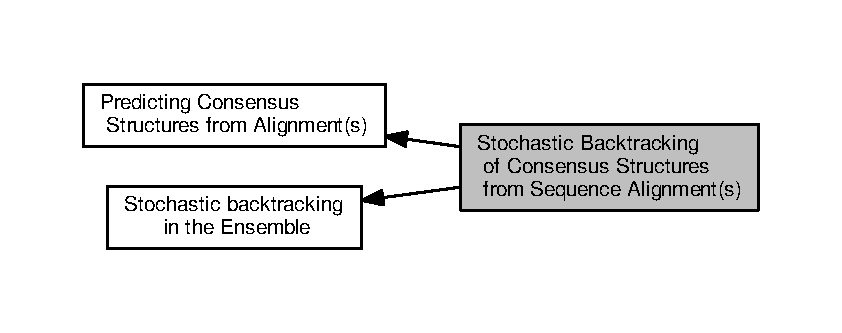
\includegraphics[width=350pt]{group__consensus__stochbt}
\end{center}
\end{figure}
\subsection*{Functions}
\begin{DoxyCompactItemize}
\item 
char $\ast$ \hyperlink{group__consensus__stochbt_ga0df40248788f0fb17ebdc59d74116d1c}{alipbacktrack} (double $\ast$prob)
\begin{DoxyCompactList}\small\item\em Sample a consensus secondary structure from the Boltzmann ensemble according its probability. \end{DoxyCompactList}\end{DoxyCompactItemize}


\subsection{Detailed Description}


\subsection{Function Documentation}
\hypertarget{group__consensus__stochbt_ga0df40248788f0fb17ebdc59d74116d1c}{}\index{Stochastic Backtracking of Consensus Structures from Sequence Alignment(s)@{Stochastic Backtracking of Consensus Structures from Sequence Alignment(s)}!alipbacktrack@{alipbacktrack}}
\index{alipbacktrack@{alipbacktrack}!Stochastic Backtracking of Consensus Structures from Sequence Alignment(s)@{Stochastic Backtracking of Consensus Structures from Sequence Alignment(s)}}
\subsubsection[{alipbacktrack}]{\setlength{\rightskip}{0pt plus 5cm}char$\ast$ alipbacktrack (
\begin{DoxyParamCaption}
\item[{double $\ast$}]{prob}
\end{DoxyParamCaption}
)}\label{group__consensus__stochbt_ga0df40248788f0fb17ebdc59d74116d1c}


{\ttfamily \#include $<$\hyperlink{alifold_8h}{Vienna\+R\+N\+A/alifold.\+h}$>$}



Sample a consensus secondary structure from the Boltzmann ensemble according its probability. 

\begin{DoxyRefDesc}{Deprecated}
\item[\hyperlink{deprecated__deprecated000023}{Deprecated}]Use \hyperlink{group__subopt__stochbt_ga0429de82e75af6c6e7508f4d273a192f}{vrna\+\_\+pbacktrack()} instead!\end{DoxyRefDesc}



\begin{DoxyParams}{Parameters}
{\em prob} & to be described (berni) \\
\hline
\end{DoxyParams}
\begin{DoxyReturn}{Returns}
A sampled consensus secondary structure in dot-\/bracket notation 
\end{DoxyReturn}

\hypertarget{group__local__fold}{}\section{Predicting Locally stable structures of large sequences}
\label{group__local__fold}\index{Predicting Locally stable structures of large sequences@{Predicting Locally stable structures of large sequences}}
Collaboration diagram for Predicting Locally stable structures of large sequences\+:
\nopagebreak
\begin{figure}[H]
\begin{center}
\leavevmode
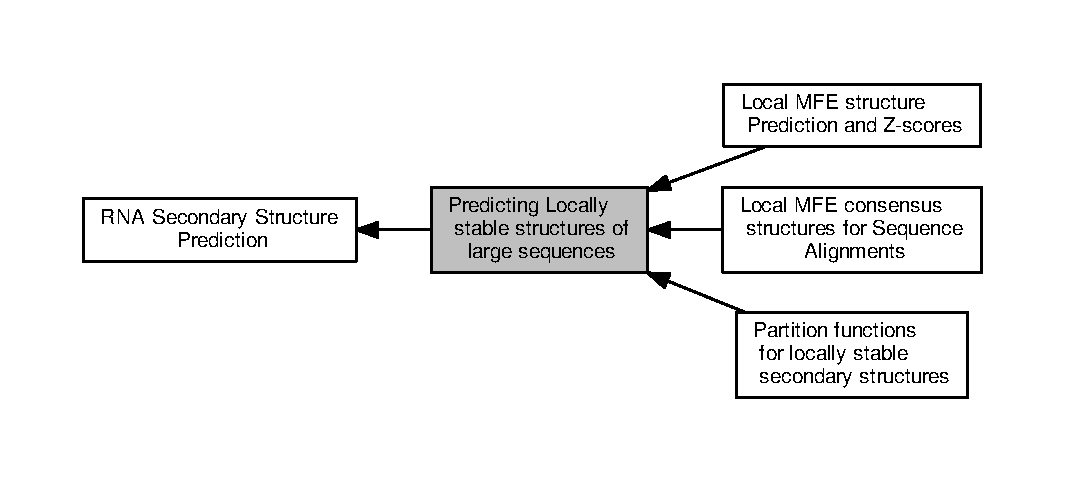
\includegraphics[width=350pt]{group__local__fold}
\end{center}
\end{figure}
\subsection*{Modules}
\begin{DoxyCompactItemize}
\item 
\hyperlink{group__local__mfe__fold}{Local M\+F\+E structure Prediction and Z-\/scores}
\item 
\hyperlink{group__local__pf__fold}{Partition functions for locally stable secondary structures}
\item 
\hyperlink{group__local__consensus__fold}{Local M\+F\+E consensus structures for Sequence Alignments}
\end{DoxyCompactItemize}
\subsection*{Files}
\begin{DoxyCompactItemize}
\item 
file \hyperlink{Lfold_8h}{Lfold.\+h}
\begin{DoxyCompactList}\small\item\em Predicting local M\+F\+E structures of large sequences. \end{DoxyCompactList}\end{DoxyCompactItemize}


\subsection{Detailed Description}
Local structures can be predicted by a modified version of the \hyperlink{group__mfe__fold__single_gaadafcb0f140795ae62e5ca027e335a9b}{fold()} algorithm that restricts the span of all base pairs. 
\hypertarget{group__local__mfe__fold}{}\section{Local M\+F\+E structure Prediction and Z-\/scores}
\label{group__local__mfe__fold}\index{Local M\+F\+E structure Prediction and Z-\/scores@{Local M\+F\+E structure Prediction and Z-\/scores}}
Collaboration diagram for Local M\+F\+E structure Prediction and Z-\/scores\+:
\nopagebreak
\begin{figure}[H]
\begin{center}
\leavevmode
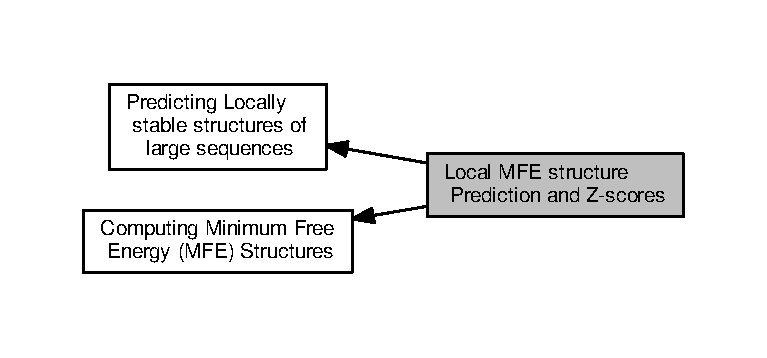
\includegraphics[width=350pt]{group__local__mfe__fold}
\end{center}
\end{figure}
\subsection*{Functions}
\begin{DoxyCompactItemize}
\item 
float \hyperlink{group__local__mfe__fold_ga4918cce52bf69c1913cda503b2ac75d8}{vrna\+\_\+\+Lfold} (const char $\ast$string, int window\+\_\+size, F\+I\+L\+E $\ast$file)
\begin{DoxyCompactList}\small\item\em Local M\+F\+E prediction using a sliding window approach (simplified interface) \end{DoxyCompactList}\item 
float \hyperlink{group__local__mfe__fold_ga27fddda5fc63eb49c861e38845fc34b4}{vrna\+\_\+\+Lfoldz} (const char $\ast$string, int window\+\_\+size, double min\+\_\+z, F\+I\+L\+E $\ast$file)
\begin{DoxyCompactList}\small\item\em Local M\+F\+E prediction using a sliding window approach with z-\/score cut-\/off (simplified interface) \end{DoxyCompactList}\item 
float \hyperlink{group__local__mfe__fold_ga16e5a70e60835bb969eaecbe6482f1be}{Lfold} (const char $\ast$string, char $\ast$structure, int maxdist)
\begin{DoxyCompactList}\small\item\em The local analog to \hyperlink{group__mfe__fold__single_gaadafcb0f140795ae62e5ca027e335a9b}{fold()}. \end{DoxyCompactList}\item 
float \hyperlink{group__local__mfe__fold_gab6d79eecc180f586679f7b85cce5cbe9}{Lfoldz} (const char $\ast$string, char $\ast$structure, int maxdist, int zsc, double min\+\_\+z)
\item 
float \hyperlink{group__local__mfe__fold_ga689df235a1915a1ad56e377383c044ce}{vrna\+\_\+mfe\+\_\+window} (\hyperlink{group__fold__compound_ga1b0cef17fd40466cef5968eaeeff6166}{vrna\+\_\+fold\+\_\+compound\+\_\+t} $\ast$vc, F\+I\+L\+E $\ast$file)
\begin{DoxyCompactList}\small\item\em Local M\+F\+E prediction using a sliding window approach. \end{DoxyCompactList}\item 
float \hyperlink{group__local__mfe__fold_gaa4f67ae94efd08d800c17f9b53423fd6}{vrna\+\_\+mfe\+\_\+window\+\_\+zscore} (\hyperlink{group__fold__compound_ga1b0cef17fd40466cef5968eaeeff6166}{vrna\+\_\+fold\+\_\+compound\+\_\+t} $\ast$vc, double min\+\_\+z, F\+I\+L\+E $\ast$file)
\begin{DoxyCompactList}\small\item\em Local M\+F\+E prediction using a sliding window approach (with z-\/score cut-\/off) \end{DoxyCompactList}\end{DoxyCompactItemize}


\subsection{Detailed Description}


\subsection{Function Documentation}
\hypertarget{group__local__mfe__fold_ga4918cce52bf69c1913cda503b2ac75d8}{}\index{Local M\+F\+E structure Prediction and Z-\/scores@{Local M\+F\+E structure Prediction and Z-\/scores}!vrna\+\_\+\+Lfold@{vrna\+\_\+\+Lfold}}
\index{vrna\+\_\+\+Lfold@{vrna\+\_\+\+Lfold}!Local M\+F\+E structure Prediction and Z-\/scores@{Local M\+F\+E structure Prediction and Z-\/scores}}
\subsubsection[{vrna\+\_\+\+Lfold}]{\setlength{\rightskip}{0pt plus 5cm}float vrna\+\_\+\+Lfold (
\begin{DoxyParamCaption}
\item[{const char $\ast$}]{string, }
\item[{int}]{window\+\_\+size, }
\item[{F\+I\+L\+E $\ast$}]{file}
\end{DoxyParamCaption}
)}\label{group__local__mfe__fold_ga4918cce52bf69c1913cda503b2ac75d8}


{\ttfamily \#include $<$\hyperlink{Lfold_8h}{Vienna\+R\+N\+A/\+Lfold.\+h}$>$}



Local M\+F\+E prediction using a sliding window approach (simplified interface) 

This simplified interface to \hyperlink{group__local__mfe__fold_ga689df235a1915a1ad56e377383c044ce}{vrna\+\_\+mfe\+\_\+window()} computes the M\+F\+E and locally optimal secondary structure using default options. Structures are predicted using a sliding window approach, where base pairs may not span outside the window. Memory required for dynamic programming (D\+P) matrices will be allocated and free\textquotesingle{}d on-\/the-\/fly. Hence, after return of this function, the recursively filled matrices are not available any more for any post-\/processing.

\begin{DoxyNote}{Note}
In case you want to use the filled D\+P matrices for any subsequent post-\/processing step, or you require other conditions than specified by the default model details, use \hyperlink{group__local__mfe__fold_ga689df235a1915a1ad56e377383c044ce}{vrna\+\_\+mfe\+\_\+window()}, and the data structure \hyperlink{group__fold__compound_ga1b0cef17fd40466cef5968eaeeff6166}{vrna\+\_\+fold\+\_\+compound\+\_\+t} instead.
\end{DoxyNote}
\begin{DoxySeeAlso}{See also}
\hyperlink{group__local__mfe__fold_ga689df235a1915a1ad56e377383c044ce}{vrna\+\_\+mfe\+\_\+window()}, \hyperlink{group__local__mfe__fold_ga27fddda5fc63eb49c861e38845fc34b4}{vrna\+\_\+\+Lfoldz()}, \hyperlink{group__local__mfe__fold_gaa4f67ae94efd08d800c17f9b53423fd6}{vrna\+\_\+mfe\+\_\+window\+\_\+zscore()}, \hyperlink{group__fold__compound_ga6601d994ba32b11511b36f68b08403be}{vrna\+\_\+fold\+\_\+compound()}, \hyperlink{group__fold__compound_ga1b0cef17fd40466cef5968eaeeff6166}{vrna\+\_\+fold\+\_\+compound\+\_\+t}
\end{DoxySeeAlso}

\begin{DoxyParams}{Parameters}
{\em string} & The nucleic acid sequence \\
\hline
{\em window\+\_\+size} & The window size for locally optimal structures \\
\hline
{\em file} & The output file handle where predictions are written to (if N\+U\+L\+L, output is written to stdout) \\
\hline
\end{DoxyParams}
\hypertarget{group__local__mfe__fold_ga27fddda5fc63eb49c861e38845fc34b4}{}\index{Local M\+F\+E structure Prediction and Z-\/scores@{Local M\+F\+E structure Prediction and Z-\/scores}!vrna\+\_\+\+Lfoldz@{vrna\+\_\+\+Lfoldz}}
\index{vrna\+\_\+\+Lfoldz@{vrna\+\_\+\+Lfoldz}!Local M\+F\+E structure Prediction and Z-\/scores@{Local M\+F\+E structure Prediction and Z-\/scores}}
\subsubsection[{vrna\+\_\+\+Lfoldz}]{\setlength{\rightskip}{0pt plus 5cm}float vrna\+\_\+\+Lfoldz (
\begin{DoxyParamCaption}
\item[{const char $\ast$}]{string, }
\item[{int}]{window\+\_\+size, }
\item[{double}]{min\+\_\+z, }
\item[{F\+I\+L\+E $\ast$}]{file}
\end{DoxyParamCaption}
)}\label{group__local__mfe__fold_ga27fddda5fc63eb49c861e38845fc34b4}


{\ttfamily \#include $<$\hyperlink{Lfold_8h}{Vienna\+R\+N\+A/\+Lfold.\+h}$>$}



Local M\+F\+E prediction using a sliding window approach with z-\/score cut-\/off (simplified interface) 

This simplified interface to \hyperlink{group__local__mfe__fold_gaa4f67ae94efd08d800c17f9b53423fd6}{vrna\+\_\+mfe\+\_\+window\+\_\+zscore()} computes the M\+F\+E and locally optimal secondary structure using default options. Structures are predicted using a sliding window approach, where base pairs may not span outside the window. Memory required for dynamic programming (D\+P) matrices will be allocated and free\textquotesingle{}d on-\/the-\/fly. Hence, after return of this function, the recursively filled matrices are not available any more for any post-\/processing. This function is the z-\/score version of \hyperlink{group__local__mfe__fold_ga4918cce52bf69c1913cda503b2ac75d8}{vrna\+\_\+\+Lfold()}, i.\+e. only predictions above a certain z-\/score cut-\/off value are printed.

\begin{DoxyNote}{Note}
In case you want to use the filled D\+P matrices for any subsequent post-\/processing step, or you require other conditions than specified by the default model details, use \hyperlink{group__local__mfe__fold_ga689df235a1915a1ad56e377383c044ce}{vrna\+\_\+mfe\+\_\+window()}, and the data structure \hyperlink{group__fold__compound_ga1b0cef17fd40466cef5968eaeeff6166}{vrna\+\_\+fold\+\_\+compound\+\_\+t} instead.
\end{DoxyNote}
\begin{DoxySeeAlso}{See also}
\hyperlink{group__local__mfe__fold_gaa4f67ae94efd08d800c17f9b53423fd6}{vrna\+\_\+mfe\+\_\+window\+\_\+zscore()}, \hyperlink{group__local__mfe__fold_ga4918cce52bf69c1913cda503b2ac75d8}{vrna\+\_\+\+Lfold()}, \hyperlink{group__local__mfe__fold_ga689df235a1915a1ad56e377383c044ce}{vrna\+\_\+mfe\+\_\+window()}, \hyperlink{group__fold__compound_ga6601d994ba32b11511b36f68b08403be}{vrna\+\_\+fold\+\_\+compound()}, \hyperlink{group__fold__compound_ga1b0cef17fd40466cef5968eaeeff6166}{vrna\+\_\+fold\+\_\+compound\+\_\+t}
\end{DoxySeeAlso}

\begin{DoxyParams}{Parameters}
{\em string} & The nucleic acid sequence \\
\hline
{\em window\+\_\+size} & The window size for locally optimal structures \\
\hline
{\em min\+\_\+z} & The minimal z-\/score for a predicted structure to appear in the output \\
\hline
{\em file} & The output file handle where predictions are written to (if N\+U\+L\+L, output is written to stdout) \\
\hline
\end{DoxyParams}
\hypertarget{group__local__mfe__fold_ga16e5a70e60835bb969eaecbe6482f1be}{}\index{Local M\+F\+E structure Prediction and Z-\/scores@{Local M\+F\+E structure Prediction and Z-\/scores}!Lfold@{Lfold}}
\index{Lfold@{Lfold}!Local M\+F\+E structure Prediction and Z-\/scores@{Local M\+F\+E structure Prediction and Z-\/scores}}
\subsubsection[{Lfold}]{\setlength{\rightskip}{0pt plus 5cm}float Lfold (
\begin{DoxyParamCaption}
\item[{const char $\ast$}]{string, }
\item[{char $\ast$}]{structure, }
\item[{int}]{maxdist}
\end{DoxyParamCaption}
)}\label{group__local__mfe__fold_ga16e5a70e60835bb969eaecbe6482f1be}


{\ttfamily \#include $<$\hyperlink{Lfold_8h}{Vienna\+R\+N\+A/\+Lfold.\+h}$>$}



The local analog to \hyperlink{group__mfe__fold__single_gaadafcb0f140795ae62e5ca027e335a9b}{fold()}. 

Computes the minimum free energy structure including only base pairs with a span smaller than \textquotesingle{}maxdist\textquotesingle{}

\begin{DoxyRefDesc}{Deprecated}
\item[\hyperlink{deprecated__deprecated000086}{Deprecated}]Use \hyperlink{group__local__mfe__fold_ga689df235a1915a1ad56e377383c044ce}{vrna\+\_\+mfe\+\_\+window()} instead! \end{DoxyRefDesc}
\hypertarget{group__local__mfe__fold_gab6d79eecc180f586679f7b85cce5cbe9}{}\index{Local M\+F\+E structure Prediction and Z-\/scores@{Local M\+F\+E structure Prediction and Z-\/scores}!Lfoldz@{Lfoldz}}
\index{Lfoldz@{Lfoldz}!Local M\+F\+E structure Prediction and Z-\/scores@{Local M\+F\+E structure Prediction and Z-\/scores}}
\subsubsection[{Lfoldz}]{\setlength{\rightskip}{0pt plus 5cm}float Lfoldz (
\begin{DoxyParamCaption}
\item[{const char $\ast$}]{string, }
\item[{char $\ast$}]{structure, }
\item[{int}]{maxdist, }
\item[{int}]{zsc, }
\item[{double}]{min\+\_\+z}
\end{DoxyParamCaption}
)}\label{group__local__mfe__fold_gab6d79eecc180f586679f7b85cce5cbe9}


{\ttfamily \#include $<$\hyperlink{Lfold_8h}{Vienna\+R\+N\+A/\+Lfold.\+h}$>$}

\begin{DoxyRefDesc}{Deprecated}
\item[\hyperlink{deprecated__deprecated000087}{Deprecated}]Use \hyperlink{group__local__mfe__fold_gaa4f67ae94efd08d800c17f9b53423fd6}{vrna\+\_\+mfe\+\_\+window\+\_\+zscore()} instead! \end{DoxyRefDesc}
\hypertarget{group__local__mfe__fold_ga689df235a1915a1ad56e377383c044ce}{}\index{Local M\+F\+E structure Prediction and Z-\/scores@{Local M\+F\+E structure Prediction and Z-\/scores}!vrna\+\_\+mfe\+\_\+window@{vrna\+\_\+mfe\+\_\+window}}
\index{vrna\+\_\+mfe\+\_\+window@{vrna\+\_\+mfe\+\_\+window}!Local M\+F\+E structure Prediction and Z-\/scores@{Local M\+F\+E structure Prediction and Z-\/scores}}
\subsubsection[{vrna\+\_\+mfe\+\_\+window}]{\setlength{\rightskip}{0pt plus 5cm}float vrna\+\_\+mfe\+\_\+window (
\begin{DoxyParamCaption}
\item[{{\bf vrna\+\_\+fold\+\_\+compound\+\_\+t} $\ast$}]{vc, }
\item[{F\+I\+L\+E $\ast$}]{file}
\end{DoxyParamCaption}
)}\label{group__local__mfe__fold_ga689df235a1915a1ad56e377383c044ce}


{\ttfamily \#include $<$\hyperlink{mfe_8h}{Vienna\+R\+N\+A/mfe.\+h}$>$}



Local M\+F\+E prediction using a sliding window approach. 

Computes minimum free energy structures using a sliding window approach, where base pairs may not span outside the window. In contrast to \hyperlink{group__mfe__fold_gabd3b147371ccf25c577f88bbbaf159fd}{vrna\+\_\+mfe()}, where a maximum base pair span may be set using the \hyperlink{group__model__details_a659e5fcc6e8c9f1a68e7de6548eef3b0}{vrna\+\_\+md\+\_\+t.\+max\+\_\+bp\+\_\+span} attribute and one globally optimal structure is predicted, this function uses a sliding window to retrieve all locally optimal structures within each window. The size of the sliding window is set in the \hyperlink{group__model__details_abea42f9229f8d8d6bcbedef316315bfc}{vrna\+\_\+md\+\_\+t.\+window\+\_\+size} attribute, prior to the retrieval of the \hyperlink{group__fold__compound_ga1b0cef17fd40466cef5968eaeeff6166}{vrna\+\_\+fold\+\_\+compound\+\_\+t} using \hyperlink{group__fold__compound_ga6601d994ba32b11511b36f68b08403be}{vrna\+\_\+fold\+\_\+compound()} with option \#\+V\+R\+N\+A\+\_\+\+O\+P\+T\+I\+O\+N\+\_\+\+W\+I\+N\+D\+O\+W

The predicted structures are written on-\/the-\/fly, either to stdout, if a N\+U\+L\+L pointer is passed as file parameter, or to the corresponding filehandle.

\begin{DoxySeeAlso}{See also}
\hyperlink{group__fold__compound_ga6601d994ba32b11511b36f68b08403be}{vrna\+\_\+fold\+\_\+compound()}, \hyperlink{group__local__mfe__fold_gaa4f67ae94efd08d800c17f9b53423fd6}{vrna\+\_\+mfe\+\_\+window\+\_\+zscore()}, \hyperlink{group__mfe__fold_gabd3b147371ccf25c577f88bbbaf159fd}{vrna\+\_\+mfe()}, \hyperlink{group__local__mfe__fold_ga4918cce52bf69c1913cda503b2ac75d8}{vrna\+\_\+\+Lfold()}, \hyperlink{group__local__mfe__fold_ga27fddda5fc63eb49c861e38845fc34b4}{vrna\+\_\+\+Lfoldz()}, \#\+V\+R\+N\+A\+\_\+\+O\+P\+T\+I\+O\+N\+\_\+\+W\+I\+N\+D\+O\+W, \hyperlink{group__model__details_a659e5fcc6e8c9f1a68e7de6548eef3b0}{vrna\+\_\+md\+\_\+t.\+max\+\_\+bp\+\_\+span}, \hyperlink{group__model__details_abea42f9229f8d8d6bcbedef316315bfc}{vrna\+\_\+md\+\_\+t.\+window\+\_\+size}
\end{DoxySeeAlso}

\begin{DoxyParams}{Parameters}
{\em vc} & The \hyperlink{group__fold__compound_ga1b0cef17fd40466cef5968eaeeff6166}{vrna\+\_\+fold\+\_\+compound\+\_\+t} with preallocated memory for the D\+P matrices \\
\hline
{\em file} & The output file handle where predictions are written to (maybe N\+U\+L\+L) \\
\hline
\end{DoxyParams}
\hypertarget{group__local__mfe__fold_gaa4f67ae94efd08d800c17f9b53423fd6}{}\index{Local M\+F\+E structure Prediction and Z-\/scores@{Local M\+F\+E structure Prediction and Z-\/scores}!vrna\+\_\+mfe\+\_\+window\+\_\+zscore@{vrna\+\_\+mfe\+\_\+window\+\_\+zscore}}
\index{vrna\+\_\+mfe\+\_\+window\+\_\+zscore@{vrna\+\_\+mfe\+\_\+window\+\_\+zscore}!Local M\+F\+E structure Prediction and Z-\/scores@{Local M\+F\+E structure Prediction and Z-\/scores}}
\subsubsection[{vrna\+\_\+mfe\+\_\+window\+\_\+zscore}]{\setlength{\rightskip}{0pt plus 5cm}float vrna\+\_\+mfe\+\_\+window\+\_\+zscore (
\begin{DoxyParamCaption}
\item[{{\bf vrna\+\_\+fold\+\_\+compound\+\_\+t} $\ast$}]{vc, }
\item[{double}]{min\+\_\+z, }
\item[{F\+I\+L\+E $\ast$}]{file}
\end{DoxyParamCaption}
)}\label{group__local__mfe__fold_gaa4f67ae94efd08d800c17f9b53423fd6}


{\ttfamily \#include $<$\hyperlink{mfe_8h}{Vienna\+R\+N\+A/mfe.\+h}$>$}



Local M\+F\+E prediction using a sliding window approach (with z-\/score cut-\/off) 

Computes minimum free energy structures using a sliding window approach, where base pairs may not span outside the window. This function is the z-\/score version of \hyperlink{group__local__mfe__fold_ga689df235a1915a1ad56e377383c044ce}{vrna\+\_\+mfe\+\_\+window()}, i.\+e. only predictions above a certain z-\/score cut-\/off value are printed. As for \hyperlink{group__local__mfe__fold_ga689df235a1915a1ad56e377383c044ce}{vrna\+\_\+mfe\+\_\+window()}, the size of the sliding window is set in the \hyperlink{group__model__details_abea42f9229f8d8d6bcbedef316315bfc}{vrna\+\_\+md\+\_\+t.\+window\+\_\+size} attribute, prior to the retrieval of the \hyperlink{group__fold__compound_ga1b0cef17fd40466cef5968eaeeff6166}{vrna\+\_\+fold\+\_\+compound\+\_\+t} using \hyperlink{group__fold__compound_ga6601d994ba32b11511b36f68b08403be}{vrna\+\_\+fold\+\_\+compound()} with option \#\+V\+R\+N\+A\+\_\+\+O\+P\+T\+I\+O\+N\+\_\+\+W\+I\+N\+D\+O\+W.

The predicted structures are written on-\/the-\/fly, either to stdout, if a N\+U\+L\+L pointer is passed as file parameter, or to the corresponding filehandle.

\begin{DoxySeeAlso}{See also}
\hyperlink{group__fold__compound_ga6601d994ba32b11511b36f68b08403be}{vrna\+\_\+fold\+\_\+compound()}, \hyperlink{group__local__mfe__fold_gaa4f67ae94efd08d800c17f9b53423fd6}{vrna\+\_\+mfe\+\_\+window\+\_\+zscore()}, \hyperlink{group__mfe__fold_gabd3b147371ccf25c577f88bbbaf159fd}{vrna\+\_\+mfe()}, \hyperlink{group__local__mfe__fold_ga4918cce52bf69c1913cda503b2ac75d8}{vrna\+\_\+\+Lfold()}, \hyperlink{group__local__mfe__fold_ga27fddda5fc63eb49c861e38845fc34b4}{vrna\+\_\+\+Lfoldz()}, \#\+V\+R\+N\+A\+\_\+\+O\+P\+T\+I\+O\+N\+\_\+\+W\+I\+N\+D\+O\+W, \hyperlink{group__model__details_a659e5fcc6e8c9f1a68e7de6548eef3b0}{vrna\+\_\+md\+\_\+t.\+max\+\_\+bp\+\_\+span}, \hyperlink{group__model__details_abea42f9229f8d8d6bcbedef316315bfc}{vrna\+\_\+md\+\_\+t.\+window\+\_\+size}
\end{DoxySeeAlso}

\begin{DoxyParams}{Parameters}
{\em vc} & The \hyperlink{group__fold__compound_ga1b0cef17fd40466cef5968eaeeff6166}{vrna\+\_\+fold\+\_\+compound\+\_\+t} with preallocated memory for the D\+P matrices \\
\hline
{\em min\+\_\+z} & The minimal z-\/score for a predicted structure to appear in the output \\
\hline
{\em file} & The output file handle where predictions are written to (maybe N\+U\+L\+L) \\
\hline
\end{DoxyParams}

\hypertarget{group__local__pf__fold}{}\section{Partition functions for locally stable secondary structures}
\label{group__local__pf__fold}\index{Partition functions for locally stable secondary structures@{Partition functions for locally stable secondary structures}}
Collaboration diagram for Partition functions for locally stable secondary structures\+:
\nopagebreak
\begin{figure}[H]
\begin{center}
\leavevmode
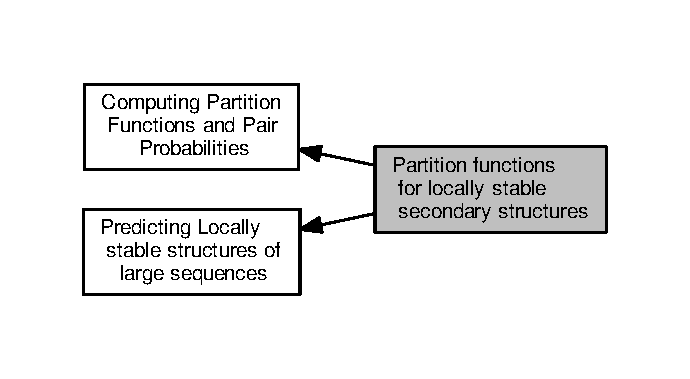
\includegraphics[width=331pt]{group__local__pf__fold}
\end{center}
\end{figure}
\subsection*{Files}
\begin{DoxyCompactItemize}
\item 
file \hyperlink{LPfold_8h}{L\+Pfold.\+h}
\begin{DoxyCompactList}\small\item\em Function declarations of partition function variants of the Lfold algorithm. \end{DoxyCompactList}\end{DoxyCompactItemize}
\subsection*{Functions}
\begin{DoxyCompactItemize}
\item 
void \hyperlink{group__local__pf__fold_ga5a019014d37fe6105131dfc2fc447880}{update\+\_\+pf\+\_\+params\+L\+P} (int length)
\item 
\hyperlink{group__data__structures_gab1d8894b43aa84cbc50b862a73785fbc}{plist} $\ast$ \hyperlink{group__local__pf__fold_ga7dcf599d07258801ea55e7d14a56908d}{pfl\+\_\+fold} (char $\ast$sequence, int win\+Size, int pair\+Size, float cutoffb, double $\ast$$\ast$p\+U, \hyperlink{group__data__structures_gab1d8894b43aa84cbc50b862a73785fbc}{plist} $\ast$$\ast$dpp2, F\+I\+L\+E $\ast$p\+Ufp, F\+I\+L\+E $\ast$spup)
\begin{DoxyCompactList}\small\item\em Compute partition functions for locally stable secondary structures. \end{DoxyCompactList}\item 
\hypertarget{group__local__pf__fold_ga14c2b82fdd5ab7a1951f1c2db4f5cf2c}{}\hyperlink{group__data__structures_gab1d8894b43aa84cbc50b862a73785fbc}{plist} $\ast$ \hyperlink{group__local__pf__fold_ga14c2b82fdd5ab7a1951f1c2db4f5cf2c}{pfl\+\_\+fold\+\_\+par} (char $\ast$sequence, int win\+Size, int pair\+Size, float cutoffb, double $\ast$$\ast$p\+U, \hyperlink{group__data__structures_gab1d8894b43aa84cbc50b862a73785fbc}{plist} $\ast$$\ast$dpp2, F\+I\+L\+E $\ast$p\+Ufp, F\+I\+L\+E $\ast$spup, \hyperlink{group__energy__parameters_ga01d8b92fe734df8d79a6169482c7d8d8}{vrna\+\_\+exp\+\_\+param\+\_\+t} $\ast$parameters)\label{group__local__pf__fold_ga14c2b82fdd5ab7a1951f1c2db4f5cf2c}

\begin{DoxyCompactList}\small\item\em Compute partition functions for locally stable secondary structures. \end{DoxyCompactList}\item 
void \hyperlink{group__local__pf__fold_ga0bcb751860bbf34e3dfee8c2fbdb3ef3}{putoutp\+U\+\_\+prob} (double $\ast$$\ast$p\+U, int length, int ulength, F\+I\+L\+E $\ast$fp, int energies)
\begin{DoxyCompactList}\small\item\em Writes the unpaired probabilities (p\+U) or opening energies into a file. \end{DoxyCompactList}\item 
void \hyperlink{group__local__pf__fold_ga9acb00ee10e96b1ca4ea394cd8bcec75}{putoutp\+U\+\_\+prob\+\_\+bin} (double $\ast$$\ast$p\+U, int length, int ulength, F\+I\+L\+E $\ast$fp, int energies)
\begin{DoxyCompactList}\small\item\em Writes the unpaired probabilities (p\+U) or opening energies into a binary file. \end{DoxyCompactList}\end{DoxyCompactItemize}


\subsection{Detailed Description}


\subsection{Function Documentation}
\hypertarget{group__local__pf__fold_ga5a019014d37fe6105131dfc2fc447880}{}\index{Partition functions for locally stable secondary structures@{Partition functions for locally stable secondary structures}!update\+\_\+pf\+\_\+params\+L\+P@{update\+\_\+pf\+\_\+params\+L\+P}}
\index{update\+\_\+pf\+\_\+params\+L\+P@{update\+\_\+pf\+\_\+params\+L\+P}!Partition functions for locally stable secondary structures@{Partition functions for locally stable secondary structures}}
\subsubsection[{update\+\_\+pf\+\_\+params\+L\+P}]{\setlength{\rightskip}{0pt plus 5cm}void update\+\_\+pf\+\_\+params\+L\+P (
\begin{DoxyParamCaption}
\item[{int}]{length}
\end{DoxyParamCaption}
)}\label{group__local__pf__fold_ga5a019014d37fe6105131dfc2fc447880}


{\ttfamily \#include $<$\hyperlink{LPfold_8h}{Vienna\+R\+N\+A/\+L\+Pfold.\+h}$>$}


\begin{DoxyParams}{Parameters}
{\em length} & \\
\hline
\end{DoxyParams}
\hypertarget{group__local__pf__fold_ga7dcf599d07258801ea55e7d14a56908d}{}\index{Partition functions for locally stable secondary structures@{Partition functions for locally stable secondary structures}!pfl\+\_\+fold@{pfl\+\_\+fold}}
\index{pfl\+\_\+fold@{pfl\+\_\+fold}!Partition functions for locally stable secondary structures@{Partition functions for locally stable secondary structures}}
\subsubsection[{pfl\+\_\+fold}]{\setlength{\rightskip}{0pt plus 5cm}{\bf plist}$\ast$ pfl\+\_\+fold (
\begin{DoxyParamCaption}
\item[{char $\ast$}]{sequence, }
\item[{int}]{win\+Size, }
\item[{int}]{pair\+Size, }
\item[{float}]{cutoffb, }
\item[{double $\ast$$\ast$}]{p\+U, }
\item[{{\bf plist} $\ast$$\ast$}]{dpp2, }
\item[{F\+I\+L\+E $\ast$}]{p\+Ufp, }
\item[{F\+I\+L\+E $\ast$}]{spup}
\end{DoxyParamCaption}
)}\label{group__local__pf__fold_ga7dcf599d07258801ea55e7d14a56908d}


{\ttfamily \#include $<$\hyperlink{LPfold_8h}{Vienna\+R\+N\+A/\+L\+Pfold.\+h}$>$}



Compute partition functions for locally stable secondary structures. 

pfl\+\_\+fold computes partition functions for every window of size \textquotesingle{}win\+Size\textquotesingle{} possible in a R\+N\+A molecule, allowing only pairs with a span smaller than \textquotesingle{}pair\+Size\textquotesingle{}. It returns the mean pair probabilities averaged over all windows containing the pair in \textquotesingle{}pl\textquotesingle{}. \textquotesingle{}win\+Size\textquotesingle{} should always be $>$= \textquotesingle{}pair\+Size\textquotesingle{}. Note that in contrast to \hyperlink{group__local__mfe__fold_ga16e5a70e60835bb969eaecbe6482f1be}{Lfold()}, bases outside of the window do not influence the structure at all. Only probabilities higher than \textquotesingle{}cutoffb\textquotesingle{} are kept.

If \textquotesingle{}p\+U\textquotesingle{} is supplied (i.\+e is not the N\+U\+L\+L pointer), \hyperlink{group__local__pf__fold_ga7dcf599d07258801ea55e7d14a56908d}{pfl\+\_\+fold()} will also compute the mean probability that regions of length \textquotesingle{}u\textquotesingle{} and smaller are unpaired. The parameter \textquotesingle{}u\textquotesingle{} is supplied in \textquotesingle{}pup\mbox{[}0\mbox{]}\mbox{[}0\mbox{]}\textquotesingle{}. On return the \textquotesingle{}pup\textquotesingle{} array will contain these probabilities, with the entry on \textquotesingle{}pup\mbox{[}x\mbox{]}\mbox{[}y\mbox{]}\textquotesingle{} containing the mean probability that x and the y-\/1 preceding bases are unpaired. The \textquotesingle{}p\+U\textquotesingle{} array needs to be large enough to hold n+1 float$\ast$ entries, where n is the sequence length.

If an array dpp2 is supplied, the probability of base pair (i,j) given that there already exists a base pair (i+1,j-\/1) is also computed and saved in this array. If p\+Ufp is given (i.\+e. not N\+U\+L\+L), p\+U is not saved but put out imediately. If spup is given (i.\+e. is not N\+U\+L\+L), the pair probabilities in pl are not saved but put out imediately.


\begin{DoxyParams}{Parameters}
{\em sequence} & R\+N\+A sequence \\
\hline
{\em win\+Size} & size of the window \\
\hline
{\em pair\+Size} & maximum size of base pair \\
\hline
{\em cutoffb} & cutoffb for base pairs \\
\hline
{\em p\+U} & array holding all unpaired probabilities \\
\hline
{\em dpp2} & array of dependent pair probabilities \\
\hline
{\em p\+Ufp} & file pointer for p\+U \\
\hline
{\em spup} & file pointer for pair probabilities \\
\hline
\end{DoxyParams}
\begin{DoxyReturn}{Returns}
list of pair probabilities 
\end{DoxyReturn}
\hypertarget{group__local__pf__fold_ga0bcb751860bbf34e3dfee8c2fbdb3ef3}{}\index{Partition functions for locally stable secondary structures@{Partition functions for locally stable secondary structures}!putoutp\+U\+\_\+prob@{putoutp\+U\+\_\+prob}}
\index{putoutp\+U\+\_\+prob@{putoutp\+U\+\_\+prob}!Partition functions for locally stable secondary structures@{Partition functions for locally stable secondary structures}}
\subsubsection[{putoutp\+U\+\_\+prob}]{\setlength{\rightskip}{0pt plus 5cm}void putoutp\+U\+\_\+prob (
\begin{DoxyParamCaption}
\item[{double $\ast$$\ast$}]{p\+U, }
\item[{int}]{length, }
\item[{int}]{ulength, }
\item[{F\+I\+L\+E $\ast$}]{fp, }
\item[{int}]{energies}
\end{DoxyParamCaption}
)}\label{group__local__pf__fold_ga0bcb751860bbf34e3dfee8c2fbdb3ef3}


{\ttfamily \#include $<$\hyperlink{LPfold_8h}{Vienna\+R\+N\+A/\+L\+Pfold.\+h}$>$}



Writes the unpaired probabilities (p\+U) or opening energies into a file. 

Can write either the unpaired probabilities (accessibilities) p\+U or the opening energies -\/log(p\+U)k\+T into a file


\begin{DoxyParams}{Parameters}
{\em p\+U} & pair probabilities \\
\hline
{\em length} & length of R\+N\+A sequence \\
\hline
{\em ulength} & maximum length of unpaired stretch \\
\hline
{\em fp} & file pointer of destination file \\
\hline
{\em energies} & switch to put out as opening energies \\
\hline
\end{DoxyParams}
\hypertarget{group__local__pf__fold_ga9acb00ee10e96b1ca4ea394cd8bcec75}{}\index{Partition functions for locally stable secondary structures@{Partition functions for locally stable secondary structures}!putoutp\+U\+\_\+prob\+\_\+bin@{putoutp\+U\+\_\+prob\+\_\+bin}}
\index{putoutp\+U\+\_\+prob\+\_\+bin@{putoutp\+U\+\_\+prob\+\_\+bin}!Partition functions for locally stable secondary structures@{Partition functions for locally stable secondary structures}}
\subsubsection[{putoutp\+U\+\_\+prob\+\_\+bin}]{\setlength{\rightskip}{0pt plus 5cm}void putoutp\+U\+\_\+prob\+\_\+bin (
\begin{DoxyParamCaption}
\item[{double $\ast$$\ast$}]{p\+U, }
\item[{int}]{length, }
\item[{int}]{ulength, }
\item[{F\+I\+L\+E $\ast$}]{fp, }
\item[{int}]{energies}
\end{DoxyParamCaption}
)}\label{group__local__pf__fold_ga9acb00ee10e96b1ca4ea394cd8bcec75}


{\ttfamily \#include $<$\hyperlink{LPfold_8h}{Vienna\+R\+N\+A/\+L\+Pfold.\+h}$>$}



Writes the unpaired probabilities (p\+U) or opening energies into a binary file. 

Can write either the unpaired probabilities (accessibilities) p\+U or the opening energies -\/log(p\+U)k\+T into a file


\begin{DoxyParams}{Parameters}
{\em p\+U} & pair probabilities \\
\hline
{\em length} & length of R\+N\+A sequence \\
\hline
{\em ulength} & maximum length of unpaired stretch \\
\hline
{\em fp} & file pointer of destination file \\
\hline
{\em energies} & switch to put out as opening energies \\
\hline
\end{DoxyParams}

\hypertarget{group__local__consensus__fold}{}\section{Local M\+F\+E consensus structures for Sequence Alignments}
\label{group__local__consensus__fold}\index{Local M\+F\+E consensus structures for Sequence Alignments@{Local M\+F\+E consensus structures for Sequence Alignments}}
Collaboration diagram for Local M\+F\+E consensus structures for Sequence Alignments\+:
\nopagebreak
\begin{figure}[H]
\begin{center}
\leavevmode
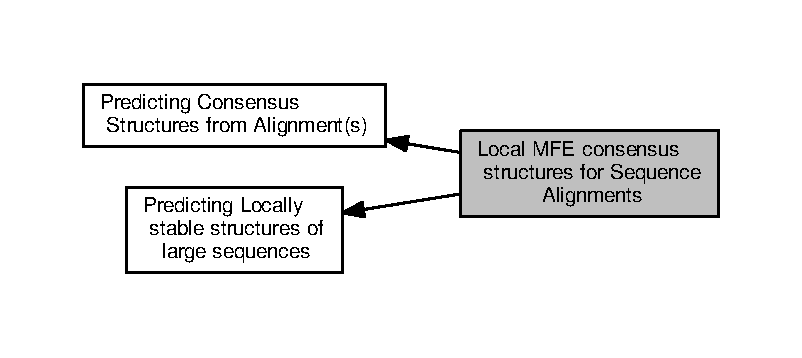
\includegraphics[width=350pt]{group__local__consensus__fold}
\end{center}
\end{figure}
\subsection*{Functions}
\begin{DoxyCompactItemize}
\item 
float \hyperlink{group__local__consensus__fold_ga20a173a3cdb83f5d1778e36c1a6b1f2b}{ali\+Lfold} (const char $\ast$$\ast$strings, char $\ast$structure, int maxdist)
\end{DoxyCompactItemize}


\subsection{Detailed Description}


\subsection{Function Documentation}
\hypertarget{group__local__consensus__fold_ga20a173a3cdb83f5d1778e36c1a6b1f2b}{}\index{Local M\+F\+E consensus structures for Sequence Alignments@{Local M\+F\+E consensus structures for Sequence Alignments}!ali\+Lfold@{ali\+Lfold}}
\index{ali\+Lfold@{ali\+Lfold}!Local M\+F\+E consensus structures for Sequence Alignments@{Local M\+F\+E consensus structures for Sequence Alignments}}
\subsubsection[{ali\+Lfold}]{\setlength{\rightskip}{0pt plus 5cm}float ali\+Lfold (
\begin{DoxyParamCaption}
\item[{const char $\ast$$\ast$}]{strings, }
\item[{char $\ast$}]{structure, }
\item[{int}]{maxdist}
\end{DoxyParamCaption}
)}\label{group__local__consensus__fold_ga20a173a3cdb83f5d1778e36c1a6b1f2b}


{\ttfamily \#include $<$\hyperlink{Lfold_8h}{Vienna\+R\+N\+A/\+Lfold.\+h}$>$}


\begin{DoxyParams}{Parameters}
{\em strings} & \\
\hline
{\em structure} & \\
\hline
{\em maxdist} & \\
\hline
\end{DoxyParams}
\begin{DoxyReturn}{Returns}

\end{DoxyReturn}

\hypertarget{group__energy__parameters__rw}{}\section{Reading/\+Writing Energy Parameter Sets from/to File}
\label{group__energy__parameters__rw}\index{Reading/\+Writing Energy Parameter Sets from/to File@{Reading/\+Writing Energy Parameter Sets from/to File}}


Read and Write energy parameter sets from and to text files.  


Collaboration diagram for Reading/\+Writing Energy Parameter Sets from/to File\+:
\nopagebreak
\begin{figure}[H]
\begin{center}
\leavevmode
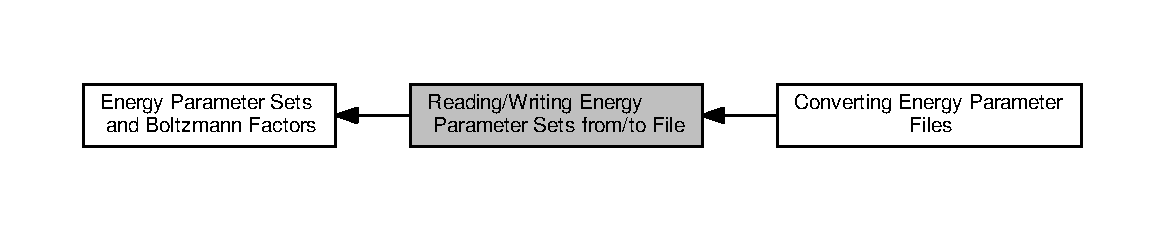
\includegraphics[width=350pt]{group__energy__parameters__rw}
\end{center}
\end{figure}
\subsection*{Modules}
\begin{DoxyCompactItemize}
\item 
\hyperlink{group__energy__parameters__convert}{Converting Energy Parameter Files}
\begin{DoxyCompactList}\small\item\em Convert energy parameter files into the latest format. \end{DoxyCompactList}\end{DoxyCompactItemize}
\subsection*{Files}
\begin{DoxyCompactItemize}
\item 
file \hyperlink{read__epars_8h}{read\+\_\+epars.\+h}
\end{DoxyCompactItemize}
\subsection*{Functions}
\begin{DoxyCompactItemize}
\item 
void \hyperlink{group__energy__parameters__rw_ga165a142a3c68fb6655c69ef4ab7cd749}{read\+\_\+parameter\+\_\+file} (const char fname\mbox{[}$\,$\mbox{]})
\begin{DoxyCompactList}\small\item\em Read energy parameters from a file. \end{DoxyCompactList}\item 
void \hyperlink{group__energy__parameters__rw_ga8a43459be386a7489feeab68dc2c6c76}{write\+\_\+parameter\+\_\+file} (const char fname\mbox{[}$\,$\mbox{]})
\begin{DoxyCompactList}\small\item\em Write energy parameters to a file. \end{DoxyCompactList}\end{DoxyCompactItemize}


\subsection{Detailed Description}
Read and Write energy parameter sets from and to text files. 

A default set of parameters, identical to the one described in \cite{mathews:2004} and \cite{turner:2010}, is compiled into the library. 

\subsection{Function Documentation}
\hypertarget{group__energy__parameters__rw_ga165a142a3c68fb6655c69ef4ab7cd749}{}\index{Reading/\+Writing Energy Parameter Sets from/to File@{Reading/\+Writing Energy Parameter Sets from/to File}!read\+\_\+parameter\+\_\+file@{read\+\_\+parameter\+\_\+file}}
\index{read\+\_\+parameter\+\_\+file@{read\+\_\+parameter\+\_\+file}!Reading/\+Writing Energy Parameter Sets from/to File@{Reading/\+Writing Energy Parameter Sets from/to File}}
\subsubsection[{read\+\_\+parameter\+\_\+file}]{\setlength{\rightskip}{0pt plus 5cm}void read\+\_\+parameter\+\_\+file (
\begin{DoxyParamCaption}
\item[{const char}]{fname\mbox{[}$\,$\mbox{]}}
\end{DoxyParamCaption}
)}\label{group__energy__parameters__rw_ga165a142a3c68fb6655c69ef4ab7cd749}


{\ttfamily \#include $<$\hyperlink{read__epars_8h}{Vienna\+R\+N\+A/read\+\_\+epars.\+h}$>$}



Read energy parameters from a file. 


\begin{DoxyParams}{Parameters}
{\em fname} & The path to the file containing the energy parameters \\
\hline
\end{DoxyParams}
\hypertarget{group__energy__parameters__rw_ga8a43459be386a7489feeab68dc2c6c76}{}\index{Reading/\+Writing Energy Parameter Sets from/to File@{Reading/\+Writing Energy Parameter Sets from/to File}!write\+\_\+parameter\+\_\+file@{write\+\_\+parameter\+\_\+file}}
\index{write\+\_\+parameter\+\_\+file@{write\+\_\+parameter\+\_\+file}!Reading/\+Writing Energy Parameter Sets from/to File@{Reading/\+Writing Energy Parameter Sets from/to File}}
\subsubsection[{write\+\_\+parameter\+\_\+file}]{\setlength{\rightskip}{0pt plus 5cm}void write\+\_\+parameter\+\_\+file (
\begin{DoxyParamCaption}
\item[{const char}]{fname\mbox{[}$\,$\mbox{]}}
\end{DoxyParamCaption}
)}\label{group__energy__parameters__rw_ga8a43459be386a7489feeab68dc2c6c76}


{\ttfamily \#include $<$\hyperlink{read__epars_8h}{Vienna\+R\+N\+A/read\+\_\+epars.\+h}$>$}



Write energy parameters to a file. 


\begin{DoxyParams}{Parameters}
{\em fname} & A filename (path) for the file where the current energy parameters will be written to \\
\hline
\end{DoxyParams}

\hypertarget{group__energy__parameters__convert}{}\section{Converting Energy Parameter Files}
\label{group__energy__parameters__convert}\index{Converting Energy Parameter Files@{Converting Energy Parameter Files}}


Convert energy parameter files into the latest format.  


Collaboration diagram for Converting Energy Parameter Files\+:
\nopagebreak
\begin{figure}[H]
\begin{center}
\leavevmode
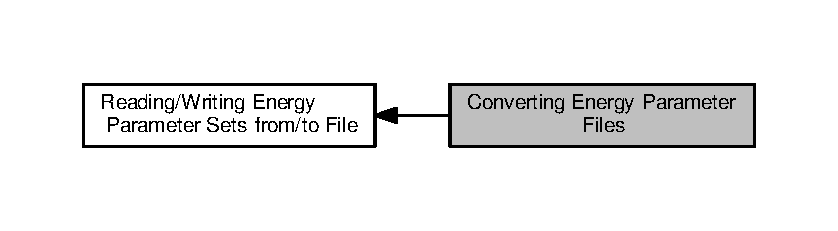
\includegraphics[width=350pt]{group__energy__parameters__convert}
\end{center}
\end{figure}
\subsection*{Files}
\begin{DoxyCompactItemize}
\item 
file \hyperlink{convert__epars_8h}{convert\+\_\+epars.\+h}
\begin{DoxyCompactList}\small\item\em Functions and definitions for energy parameter file format conversion. \end{DoxyCompactList}\end{DoxyCompactItemize}
\subsection*{Macros}
\begin{DoxyCompactItemize}
\item 
\#define \hyperlink{group__energy__parameters__convert_ga8dc6aee5a806c49b71557152f9616bc4}{V\+R\+N\+A\+\_\+\+C\+O\+N\+V\+E\+R\+T\+\_\+\+O\+U\+T\+P\+U\+T\+\_\+\+A\+L\+L}~1\+U
\item 
\#define \hyperlink{group__energy__parameters__convert_gaf66fe2cb11dfcfd32d791049c254a8a4}{V\+R\+N\+A\+\_\+\+C\+O\+N\+V\+E\+R\+T\+\_\+\+O\+U\+T\+P\+U\+T\+\_\+\+H\+P}~2\+U
\item 
\#define \hyperlink{group__energy__parameters__convert_gad23522d63f8d4c50d5a5deee9bee3ef2}{V\+R\+N\+A\+\_\+\+C\+O\+N\+V\+E\+R\+T\+\_\+\+O\+U\+T\+P\+U\+T\+\_\+\+S\+T\+A\+C\+K}~4\+U
\item 
\#define \hyperlink{group__energy__parameters__convert_gaa892c7b4957459090f3e08da298cc347}{V\+R\+N\+A\+\_\+\+C\+O\+N\+V\+E\+R\+T\+\_\+\+O\+U\+T\+P\+U\+T\+\_\+\+M\+M\+\_\+\+H\+P}~8\+U
\item 
\#define \hyperlink{group__energy__parameters__convert_ga4ff223fb1f9c62cd92d9ab811ad03d55}{V\+R\+N\+A\+\_\+\+C\+O\+N\+V\+E\+R\+T\+\_\+\+O\+U\+T\+P\+U\+T\+\_\+\+M\+M\+\_\+\+I\+N\+T}~16\+U
\item 
\#define \hyperlink{group__energy__parameters__convert_gaf5d3743219f83c6348155cd81e755bbb}{V\+R\+N\+A\+\_\+\+C\+O\+N\+V\+E\+R\+T\+\_\+\+O\+U\+T\+P\+U\+T\+\_\+\+M\+M\+\_\+\+I\+N\+T\+\_\+1\+N}~32\+U
\item 
\#define \hyperlink{group__energy__parameters__convert_ga78382ec622ba99e0ac2262317bdd7316}{V\+R\+N\+A\+\_\+\+C\+O\+N\+V\+E\+R\+T\+\_\+\+O\+U\+T\+P\+U\+T\+\_\+\+M\+M\+\_\+\+I\+N\+T\+\_\+23}~64\+U
\item 
\#define \hyperlink{group__energy__parameters__convert_gae67af9f1cdf7baf2865481282a5d1034}{V\+R\+N\+A\+\_\+\+C\+O\+N\+V\+E\+R\+T\+\_\+\+O\+U\+T\+P\+U\+T\+\_\+\+M\+M\+\_\+\+M\+U\+L\+T\+I}~128\+U
\item 
\#define \hyperlink{group__energy__parameters__convert_gaf14ead7ef1fdbe725ade653750fc51e3}{V\+R\+N\+A\+\_\+\+C\+O\+N\+V\+E\+R\+T\+\_\+\+O\+U\+T\+P\+U\+T\+\_\+\+M\+M\+\_\+\+E\+X\+T}~256\+U
\item 
\#define \hyperlink{group__energy__parameters__convert_ga036ffd996d8c8a9acf631760dd1da24b}{V\+R\+N\+A\+\_\+\+C\+O\+N\+V\+E\+R\+T\+\_\+\+O\+U\+T\+P\+U\+T\+\_\+\+D\+A\+N\+G\+L\+E5}~512\+U
\item 
\#define \hyperlink{group__energy__parameters__convert_ga34a8a5479ef885834ef32f3fb43d79bc}{V\+R\+N\+A\+\_\+\+C\+O\+N\+V\+E\+R\+T\+\_\+\+O\+U\+T\+P\+U\+T\+\_\+\+D\+A\+N\+G\+L\+E3}~1024\+U
\item 
\#define \hyperlink{group__energy__parameters__convert_ga079aafefd5f8ab57ee5120099a34bd25}{V\+R\+N\+A\+\_\+\+C\+O\+N\+V\+E\+R\+T\+\_\+\+O\+U\+T\+P\+U\+T\+\_\+\+I\+N\+T\+\_\+11}~2048\+U
\item 
\#define \hyperlink{group__energy__parameters__convert_gacf770881d9034431ebe741642342a1f9}{V\+R\+N\+A\+\_\+\+C\+O\+N\+V\+E\+R\+T\+\_\+\+O\+U\+T\+P\+U\+T\+\_\+\+I\+N\+T\+\_\+21}~4096\+U
\item 
\#define \hyperlink{group__energy__parameters__convert_gaa307671e2631cdacad9cbe4c6583b05f}{V\+R\+N\+A\+\_\+\+C\+O\+N\+V\+E\+R\+T\+\_\+\+O\+U\+T\+P\+U\+T\+\_\+\+I\+N\+T\+\_\+22}~8192\+U
\item 
\#define \hyperlink{group__energy__parameters__convert_ga7092fe0be4de6f02cc0bf08e81af726a}{V\+R\+N\+A\+\_\+\+C\+O\+N\+V\+E\+R\+T\+\_\+\+O\+U\+T\+P\+U\+T\+\_\+\+B\+U\+L\+G\+E}~16384\+U
\item 
\#define \hyperlink{group__energy__parameters__convert_gac5c2289fdf8ff1b980976d1613ff943a}{V\+R\+N\+A\+\_\+\+C\+O\+N\+V\+E\+R\+T\+\_\+\+O\+U\+T\+P\+U\+T\+\_\+\+I\+N\+T}~32768\+U
\item 
\#define \hyperlink{group__energy__parameters__convert_gaf2c8755d64eff3852aa45df9ac80a4fe}{V\+R\+N\+A\+\_\+\+C\+O\+N\+V\+E\+R\+T\+\_\+\+O\+U\+T\+P\+U\+T\+\_\+\+M\+L}~65536\+U
\item 
\#define \hyperlink{group__energy__parameters__convert_ga46d5b1535ae86060b6317565b7c6b40b}{V\+R\+N\+A\+\_\+\+C\+O\+N\+V\+E\+R\+T\+\_\+\+O\+U\+T\+P\+U\+T\+\_\+\+M\+I\+S\+C}~131072\+U
\item 
\#define \hyperlink{group__energy__parameters__convert_gaa1ff48a79642d69579d1766561ec6db6}{V\+R\+N\+A\+\_\+\+C\+O\+N\+V\+E\+R\+T\+\_\+\+O\+U\+T\+P\+U\+T\+\_\+\+S\+P\+E\+C\+I\+A\+L\+\_\+\+H\+P}~262144\+U
\item 
\#define \hyperlink{group__energy__parameters__convert_ga0d4e8a836bb4864ab5129c085dbf592d}{V\+R\+N\+A\+\_\+\+C\+O\+N\+V\+E\+R\+T\+\_\+\+O\+U\+T\+P\+U\+T\+\_\+\+V\+A\+N\+I\+L\+L\+A}~524288\+U
\item 
\#define \hyperlink{group__energy__parameters__convert_ga2eb0462f16939ddacdaf751a88d675ce}{V\+R\+N\+A\+\_\+\+C\+O\+N\+V\+E\+R\+T\+\_\+\+O\+U\+T\+P\+U\+T\+\_\+\+N\+I\+N\+I\+O}~1048576\+U
\item 
\#define \hyperlink{group__energy__parameters__convert_gac86976e9c2a55b3a6481ea60044f6098}{V\+R\+N\+A\+\_\+\+C\+O\+N\+V\+E\+R\+T\+\_\+\+O\+U\+T\+P\+U\+T\+\_\+\+D\+U\+M\+P}~2097152\+U
\end{DoxyCompactItemize}
\subsection*{Functions}
\begin{DoxyCompactItemize}
\item 
void \hyperlink{group__energy__parameters__convert_gafbe538bc4eb2cf2a33326e1010005f8a}{convert\+\_\+parameter\+\_\+file} (const char $\ast$iname, const char $\ast$oname, unsigned int options)
\end{DoxyCompactItemize}


\subsection{Detailed Description}
Convert energy parameter files into the latest format. 

To preserve some backward compatibility the R\+N\+Alib also provides functions to convert energy parameter files from the format used in version 1.\+4-\/1.\+8 into the new format used since version 2.\+0 

\subsection{Macro Definition Documentation}
\hypertarget{group__energy__parameters__convert_ga8dc6aee5a806c49b71557152f9616bc4}{}\index{Converting Energy Parameter Files@{Converting Energy Parameter Files}!V\+R\+N\+A\+\_\+\+C\+O\+N\+V\+E\+R\+T\+\_\+\+O\+U\+T\+P\+U\+T\+\_\+\+A\+L\+L@{V\+R\+N\+A\+\_\+\+C\+O\+N\+V\+E\+R\+T\+\_\+\+O\+U\+T\+P\+U\+T\+\_\+\+A\+L\+L}}
\index{V\+R\+N\+A\+\_\+\+C\+O\+N\+V\+E\+R\+T\+\_\+\+O\+U\+T\+P\+U\+T\+\_\+\+A\+L\+L@{V\+R\+N\+A\+\_\+\+C\+O\+N\+V\+E\+R\+T\+\_\+\+O\+U\+T\+P\+U\+T\+\_\+\+A\+L\+L}!Converting Energy Parameter Files@{Converting Energy Parameter Files}}
\subsubsection[{V\+R\+N\+A\+\_\+\+C\+O\+N\+V\+E\+R\+T\+\_\+\+O\+U\+T\+P\+U\+T\+\_\+\+A\+L\+L}]{\setlength{\rightskip}{0pt plus 5cm}\#define V\+R\+N\+A\+\_\+\+C\+O\+N\+V\+E\+R\+T\+\_\+\+O\+U\+T\+P\+U\+T\+\_\+\+A\+L\+L~1\+U}\label{group__energy__parameters__convert_ga8dc6aee5a806c49b71557152f9616bc4}


{\ttfamily \#include $<$\hyperlink{convert__epars_8h}{Vienna\+R\+N\+A/convert\+\_\+epars.\+h}$>$}

Flag to indicate printing of a complete parameter set \hypertarget{group__energy__parameters__convert_gaf66fe2cb11dfcfd32d791049c254a8a4}{}\index{Converting Energy Parameter Files@{Converting Energy Parameter Files}!V\+R\+N\+A\+\_\+\+C\+O\+N\+V\+E\+R\+T\+\_\+\+O\+U\+T\+P\+U\+T\+\_\+\+H\+P@{V\+R\+N\+A\+\_\+\+C\+O\+N\+V\+E\+R\+T\+\_\+\+O\+U\+T\+P\+U\+T\+\_\+\+H\+P}}
\index{V\+R\+N\+A\+\_\+\+C\+O\+N\+V\+E\+R\+T\+\_\+\+O\+U\+T\+P\+U\+T\+\_\+\+H\+P@{V\+R\+N\+A\+\_\+\+C\+O\+N\+V\+E\+R\+T\+\_\+\+O\+U\+T\+P\+U\+T\+\_\+\+H\+P}!Converting Energy Parameter Files@{Converting Energy Parameter Files}}
\subsubsection[{V\+R\+N\+A\+\_\+\+C\+O\+N\+V\+E\+R\+T\+\_\+\+O\+U\+T\+P\+U\+T\+\_\+\+H\+P}]{\setlength{\rightskip}{0pt plus 5cm}\#define V\+R\+N\+A\+\_\+\+C\+O\+N\+V\+E\+R\+T\+\_\+\+O\+U\+T\+P\+U\+T\+\_\+\+H\+P~2\+U}\label{group__energy__parameters__convert_gaf66fe2cb11dfcfd32d791049c254a8a4}


{\ttfamily \#include $<$\hyperlink{convert__epars_8h}{Vienna\+R\+N\+A/convert\+\_\+epars.\+h}$>$}

Flag to indicate printing of hairpin contributions \hypertarget{group__energy__parameters__convert_gad23522d63f8d4c50d5a5deee9bee3ef2}{}\index{Converting Energy Parameter Files@{Converting Energy Parameter Files}!V\+R\+N\+A\+\_\+\+C\+O\+N\+V\+E\+R\+T\+\_\+\+O\+U\+T\+P\+U\+T\+\_\+\+S\+T\+A\+C\+K@{V\+R\+N\+A\+\_\+\+C\+O\+N\+V\+E\+R\+T\+\_\+\+O\+U\+T\+P\+U\+T\+\_\+\+S\+T\+A\+C\+K}}
\index{V\+R\+N\+A\+\_\+\+C\+O\+N\+V\+E\+R\+T\+\_\+\+O\+U\+T\+P\+U\+T\+\_\+\+S\+T\+A\+C\+K@{V\+R\+N\+A\+\_\+\+C\+O\+N\+V\+E\+R\+T\+\_\+\+O\+U\+T\+P\+U\+T\+\_\+\+S\+T\+A\+C\+K}!Converting Energy Parameter Files@{Converting Energy Parameter Files}}
\subsubsection[{V\+R\+N\+A\+\_\+\+C\+O\+N\+V\+E\+R\+T\+\_\+\+O\+U\+T\+P\+U\+T\+\_\+\+S\+T\+A\+C\+K}]{\setlength{\rightskip}{0pt plus 5cm}\#define V\+R\+N\+A\+\_\+\+C\+O\+N\+V\+E\+R\+T\+\_\+\+O\+U\+T\+P\+U\+T\+\_\+\+S\+T\+A\+C\+K~4\+U}\label{group__energy__parameters__convert_gad23522d63f8d4c50d5a5deee9bee3ef2}


{\ttfamily \#include $<$\hyperlink{convert__epars_8h}{Vienna\+R\+N\+A/convert\+\_\+epars.\+h}$>$}

Flag to indicate printing of base pair stack contributions \hypertarget{group__energy__parameters__convert_gaa892c7b4957459090f3e08da298cc347}{}\index{Converting Energy Parameter Files@{Converting Energy Parameter Files}!V\+R\+N\+A\+\_\+\+C\+O\+N\+V\+E\+R\+T\+\_\+\+O\+U\+T\+P\+U\+T\+\_\+\+M\+M\+\_\+\+H\+P@{V\+R\+N\+A\+\_\+\+C\+O\+N\+V\+E\+R\+T\+\_\+\+O\+U\+T\+P\+U\+T\+\_\+\+M\+M\+\_\+\+H\+P}}
\index{V\+R\+N\+A\+\_\+\+C\+O\+N\+V\+E\+R\+T\+\_\+\+O\+U\+T\+P\+U\+T\+\_\+\+M\+M\+\_\+\+H\+P@{V\+R\+N\+A\+\_\+\+C\+O\+N\+V\+E\+R\+T\+\_\+\+O\+U\+T\+P\+U\+T\+\_\+\+M\+M\+\_\+\+H\+P}!Converting Energy Parameter Files@{Converting Energy Parameter Files}}
\subsubsection[{V\+R\+N\+A\+\_\+\+C\+O\+N\+V\+E\+R\+T\+\_\+\+O\+U\+T\+P\+U\+T\+\_\+\+M\+M\+\_\+\+H\+P}]{\setlength{\rightskip}{0pt plus 5cm}\#define V\+R\+N\+A\+\_\+\+C\+O\+N\+V\+E\+R\+T\+\_\+\+O\+U\+T\+P\+U\+T\+\_\+\+M\+M\+\_\+\+H\+P~8\+U}\label{group__energy__parameters__convert_gaa892c7b4957459090f3e08da298cc347}


{\ttfamily \#include $<$\hyperlink{convert__epars_8h}{Vienna\+R\+N\+A/convert\+\_\+epars.\+h}$>$}

Flag to indicate printing of hairpin mismatch contribution \hypertarget{group__energy__parameters__convert_ga4ff223fb1f9c62cd92d9ab811ad03d55}{}\index{Converting Energy Parameter Files@{Converting Energy Parameter Files}!V\+R\+N\+A\+\_\+\+C\+O\+N\+V\+E\+R\+T\+\_\+\+O\+U\+T\+P\+U\+T\+\_\+\+M\+M\+\_\+\+I\+N\+T@{V\+R\+N\+A\+\_\+\+C\+O\+N\+V\+E\+R\+T\+\_\+\+O\+U\+T\+P\+U\+T\+\_\+\+M\+M\+\_\+\+I\+N\+T}}
\index{V\+R\+N\+A\+\_\+\+C\+O\+N\+V\+E\+R\+T\+\_\+\+O\+U\+T\+P\+U\+T\+\_\+\+M\+M\+\_\+\+I\+N\+T@{V\+R\+N\+A\+\_\+\+C\+O\+N\+V\+E\+R\+T\+\_\+\+O\+U\+T\+P\+U\+T\+\_\+\+M\+M\+\_\+\+I\+N\+T}!Converting Energy Parameter Files@{Converting Energy Parameter Files}}
\subsubsection[{V\+R\+N\+A\+\_\+\+C\+O\+N\+V\+E\+R\+T\+\_\+\+O\+U\+T\+P\+U\+T\+\_\+\+M\+M\+\_\+\+I\+N\+T}]{\setlength{\rightskip}{0pt plus 5cm}\#define V\+R\+N\+A\+\_\+\+C\+O\+N\+V\+E\+R\+T\+\_\+\+O\+U\+T\+P\+U\+T\+\_\+\+M\+M\+\_\+\+I\+N\+T~16\+U}\label{group__energy__parameters__convert_ga4ff223fb1f9c62cd92d9ab811ad03d55}


{\ttfamily \#include $<$\hyperlink{convert__epars_8h}{Vienna\+R\+N\+A/convert\+\_\+epars.\+h}$>$}

Flag to indicate printing of interior loop mismatch contribution \hypertarget{group__energy__parameters__convert_gaf5d3743219f83c6348155cd81e755bbb}{}\index{Converting Energy Parameter Files@{Converting Energy Parameter Files}!V\+R\+N\+A\+\_\+\+C\+O\+N\+V\+E\+R\+T\+\_\+\+O\+U\+T\+P\+U\+T\+\_\+\+M\+M\+\_\+\+I\+N\+T\+\_\+1\+N@{V\+R\+N\+A\+\_\+\+C\+O\+N\+V\+E\+R\+T\+\_\+\+O\+U\+T\+P\+U\+T\+\_\+\+M\+M\+\_\+\+I\+N\+T\+\_\+1\+N}}
\index{V\+R\+N\+A\+\_\+\+C\+O\+N\+V\+E\+R\+T\+\_\+\+O\+U\+T\+P\+U\+T\+\_\+\+M\+M\+\_\+\+I\+N\+T\+\_\+1\+N@{V\+R\+N\+A\+\_\+\+C\+O\+N\+V\+E\+R\+T\+\_\+\+O\+U\+T\+P\+U\+T\+\_\+\+M\+M\+\_\+\+I\+N\+T\+\_\+1\+N}!Converting Energy Parameter Files@{Converting Energy Parameter Files}}
\subsubsection[{V\+R\+N\+A\+\_\+\+C\+O\+N\+V\+E\+R\+T\+\_\+\+O\+U\+T\+P\+U\+T\+\_\+\+M\+M\+\_\+\+I\+N\+T\+\_\+1\+N}]{\setlength{\rightskip}{0pt plus 5cm}\#define V\+R\+N\+A\+\_\+\+C\+O\+N\+V\+E\+R\+T\+\_\+\+O\+U\+T\+P\+U\+T\+\_\+\+M\+M\+\_\+\+I\+N\+T\+\_\+1\+N~32\+U}\label{group__energy__parameters__convert_gaf5d3743219f83c6348155cd81e755bbb}


{\ttfamily \#include $<$\hyperlink{convert__epars_8h}{Vienna\+R\+N\+A/convert\+\_\+epars.\+h}$>$}

Flag to indicate printing of 1\+:n interior loop mismatch contribution \hypertarget{group__energy__parameters__convert_ga78382ec622ba99e0ac2262317bdd7316}{}\index{Converting Energy Parameter Files@{Converting Energy Parameter Files}!V\+R\+N\+A\+\_\+\+C\+O\+N\+V\+E\+R\+T\+\_\+\+O\+U\+T\+P\+U\+T\+\_\+\+M\+M\+\_\+\+I\+N\+T\+\_\+23@{V\+R\+N\+A\+\_\+\+C\+O\+N\+V\+E\+R\+T\+\_\+\+O\+U\+T\+P\+U\+T\+\_\+\+M\+M\+\_\+\+I\+N\+T\+\_\+23}}
\index{V\+R\+N\+A\+\_\+\+C\+O\+N\+V\+E\+R\+T\+\_\+\+O\+U\+T\+P\+U\+T\+\_\+\+M\+M\+\_\+\+I\+N\+T\+\_\+23@{V\+R\+N\+A\+\_\+\+C\+O\+N\+V\+E\+R\+T\+\_\+\+O\+U\+T\+P\+U\+T\+\_\+\+M\+M\+\_\+\+I\+N\+T\+\_\+23}!Converting Energy Parameter Files@{Converting Energy Parameter Files}}
\subsubsection[{V\+R\+N\+A\+\_\+\+C\+O\+N\+V\+E\+R\+T\+\_\+\+O\+U\+T\+P\+U\+T\+\_\+\+M\+M\+\_\+\+I\+N\+T\+\_\+23}]{\setlength{\rightskip}{0pt plus 5cm}\#define V\+R\+N\+A\+\_\+\+C\+O\+N\+V\+E\+R\+T\+\_\+\+O\+U\+T\+P\+U\+T\+\_\+\+M\+M\+\_\+\+I\+N\+T\+\_\+23~64\+U}\label{group__energy__parameters__convert_ga78382ec622ba99e0ac2262317bdd7316}


{\ttfamily \#include $<$\hyperlink{convert__epars_8h}{Vienna\+R\+N\+A/convert\+\_\+epars.\+h}$>$}

Flag to indicate printing of 2\+:3 interior loop mismatch contribution \hypertarget{group__energy__parameters__convert_gae67af9f1cdf7baf2865481282a5d1034}{}\index{Converting Energy Parameter Files@{Converting Energy Parameter Files}!V\+R\+N\+A\+\_\+\+C\+O\+N\+V\+E\+R\+T\+\_\+\+O\+U\+T\+P\+U\+T\+\_\+\+M\+M\+\_\+\+M\+U\+L\+T\+I@{V\+R\+N\+A\+\_\+\+C\+O\+N\+V\+E\+R\+T\+\_\+\+O\+U\+T\+P\+U\+T\+\_\+\+M\+M\+\_\+\+M\+U\+L\+T\+I}}
\index{V\+R\+N\+A\+\_\+\+C\+O\+N\+V\+E\+R\+T\+\_\+\+O\+U\+T\+P\+U\+T\+\_\+\+M\+M\+\_\+\+M\+U\+L\+T\+I@{V\+R\+N\+A\+\_\+\+C\+O\+N\+V\+E\+R\+T\+\_\+\+O\+U\+T\+P\+U\+T\+\_\+\+M\+M\+\_\+\+M\+U\+L\+T\+I}!Converting Energy Parameter Files@{Converting Energy Parameter Files}}
\subsubsection[{V\+R\+N\+A\+\_\+\+C\+O\+N\+V\+E\+R\+T\+\_\+\+O\+U\+T\+P\+U\+T\+\_\+\+M\+M\+\_\+\+M\+U\+L\+T\+I}]{\setlength{\rightskip}{0pt plus 5cm}\#define V\+R\+N\+A\+\_\+\+C\+O\+N\+V\+E\+R\+T\+\_\+\+O\+U\+T\+P\+U\+T\+\_\+\+M\+M\+\_\+\+M\+U\+L\+T\+I~128\+U}\label{group__energy__parameters__convert_gae67af9f1cdf7baf2865481282a5d1034}


{\ttfamily \#include $<$\hyperlink{convert__epars_8h}{Vienna\+R\+N\+A/convert\+\_\+epars.\+h}$>$}

Flag to indicate printing of multi loop mismatch contribution \hypertarget{group__energy__parameters__convert_gaf14ead7ef1fdbe725ade653750fc51e3}{}\index{Converting Energy Parameter Files@{Converting Energy Parameter Files}!V\+R\+N\+A\+\_\+\+C\+O\+N\+V\+E\+R\+T\+\_\+\+O\+U\+T\+P\+U\+T\+\_\+\+M\+M\+\_\+\+E\+X\+T@{V\+R\+N\+A\+\_\+\+C\+O\+N\+V\+E\+R\+T\+\_\+\+O\+U\+T\+P\+U\+T\+\_\+\+M\+M\+\_\+\+E\+X\+T}}
\index{V\+R\+N\+A\+\_\+\+C\+O\+N\+V\+E\+R\+T\+\_\+\+O\+U\+T\+P\+U\+T\+\_\+\+M\+M\+\_\+\+E\+X\+T@{V\+R\+N\+A\+\_\+\+C\+O\+N\+V\+E\+R\+T\+\_\+\+O\+U\+T\+P\+U\+T\+\_\+\+M\+M\+\_\+\+E\+X\+T}!Converting Energy Parameter Files@{Converting Energy Parameter Files}}
\subsubsection[{V\+R\+N\+A\+\_\+\+C\+O\+N\+V\+E\+R\+T\+\_\+\+O\+U\+T\+P\+U\+T\+\_\+\+M\+M\+\_\+\+E\+X\+T}]{\setlength{\rightskip}{0pt plus 5cm}\#define V\+R\+N\+A\+\_\+\+C\+O\+N\+V\+E\+R\+T\+\_\+\+O\+U\+T\+P\+U\+T\+\_\+\+M\+M\+\_\+\+E\+X\+T~256\+U}\label{group__energy__parameters__convert_gaf14ead7ef1fdbe725ade653750fc51e3}


{\ttfamily \#include $<$\hyperlink{convert__epars_8h}{Vienna\+R\+N\+A/convert\+\_\+epars.\+h}$>$}

Flag to indicate printing of exterior loop mismatch contribution \hypertarget{group__energy__parameters__convert_ga036ffd996d8c8a9acf631760dd1da24b}{}\index{Converting Energy Parameter Files@{Converting Energy Parameter Files}!V\+R\+N\+A\+\_\+\+C\+O\+N\+V\+E\+R\+T\+\_\+\+O\+U\+T\+P\+U\+T\+\_\+\+D\+A\+N\+G\+L\+E5@{V\+R\+N\+A\+\_\+\+C\+O\+N\+V\+E\+R\+T\+\_\+\+O\+U\+T\+P\+U\+T\+\_\+\+D\+A\+N\+G\+L\+E5}}
\index{V\+R\+N\+A\+\_\+\+C\+O\+N\+V\+E\+R\+T\+\_\+\+O\+U\+T\+P\+U\+T\+\_\+\+D\+A\+N\+G\+L\+E5@{V\+R\+N\+A\+\_\+\+C\+O\+N\+V\+E\+R\+T\+\_\+\+O\+U\+T\+P\+U\+T\+\_\+\+D\+A\+N\+G\+L\+E5}!Converting Energy Parameter Files@{Converting Energy Parameter Files}}
\subsubsection[{V\+R\+N\+A\+\_\+\+C\+O\+N\+V\+E\+R\+T\+\_\+\+O\+U\+T\+P\+U\+T\+\_\+\+D\+A\+N\+G\+L\+E5}]{\setlength{\rightskip}{0pt plus 5cm}\#define V\+R\+N\+A\+\_\+\+C\+O\+N\+V\+E\+R\+T\+\_\+\+O\+U\+T\+P\+U\+T\+\_\+\+D\+A\+N\+G\+L\+E5~512\+U}\label{group__energy__parameters__convert_ga036ffd996d8c8a9acf631760dd1da24b}


{\ttfamily \#include $<$\hyperlink{convert__epars_8h}{Vienna\+R\+N\+A/convert\+\_\+epars.\+h}$>$}

Flag to indicate printing of 5\textquotesingle{} dangle conctribution \hypertarget{group__energy__parameters__convert_ga34a8a5479ef885834ef32f3fb43d79bc}{}\index{Converting Energy Parameter Files@{Converting Energy Parameter Files}!V\+R\+N\+A\+\_\+\+C\+O\+N\+V\+E\+R\+T\+\_\+\+O\+U\+T\+P\+U\+T\+\_\+\+D\+A\+N\+G\+L\+E3@{V\+R\+N\+A\+\_\+\+C\+O\+N\+V\+E\+R\+T\+\_\+\+O\+U\+T\+P\+U\+T\+\_\+\+D\+A\+N\+G\+L\+E3}}
\index{V\+R\+N\+A\+\_\+\+C\+O\+N\+V\+E\+R\+T\+\_\+\+O\+U\+T\+P\+U\+T\+\_\+\+D\+A\+N\+G\+L\+E3@{V\+R\+N\+A\+\_\+\+C\+O\+N\+V\+E\+R\+T\+\_\+\+O\+U\+T\+P\+U\+T\+\_\+\+D\+A\+N\+G\+L\+E3}!Converting Energy Parameter Files@{Converting Energy Parameter Files}}
\subsubsection[{V\+R\+N\+A\+\_\+\+C\+O\+N\+V\+E\+R\+T\+\_\+\+O\+U\+T\+P\+U\+T\+\_\+\+D\+A\+N\+G\+L\+E3}]{\setlength{\rightskip}{0pt plus 5cm}\#define V\+R\+N\+A\+\_\+\+C\+O\+N\+V\+E\+R\+T\+\_\+\+O\+U\+T\+P\+U\+T\+\_\+\+D\+A\+N\+G\+L\+E3~1024\+U}\label{group__energy__parameters__convert_ga34a8a5479ef885834ef32f3fb43d79bc}


{\ttfamily \#include $<$\hyperlink{convert__epars_8h}{Vienna\+R\+N\+A/convert\+\_\+epars.\+h}$>$}

Flag to indicate printing of 3\textquotesingle{} dangle contribution \hypertarget{group__energy__parameters__convert_ga079aafefd5f8ab57ee5120099a34bd25}{}\index{Converting Energy Parameter Files@{Converting Energy Parameter Files}!V\+R\+N\+A\+\_\+\+C\+O\+N\+V\+E\+R\+T\+\_\+\+O\+U\+T\+P\+U\+T\+\_\+\+I\+N\+T\+\_\+11@{V\+R\+N\+A\+\_\+\+C\+O\+N\+V\+E\+R\+T\+\_\+\+O\+U\+T\+P\+U\+T\+\_\+\+I\+N\+T\+\_\+11}}
\index{V\+R\+N\+A\+\_\+\+C\+O\+N\+V\+E\+R\+T\+\_\+\+O\+U\+T\+P\+U\+T\+\_\+\+I\+N\+T\+\_\+11@{V\+R\+N\+A\+\_\+\+C\+O\+N\+V\+E\+R\+T\+\_\+\+O\+U\+T\+P\+U\+T\+\_\+\+I\+N\+T\+\_\+11}!Converting Energy Parameter Files@{Converting Energy Parameter Files}}
\subsubsection[{V\+R\+N\+A\+\_\+\+C\+O\+N\+V\+E\+R\+T\+\_\+\+O\+U\+T\+P\+U\+T\+\_\+\+I\+N\+T\+\_\+11}]{\setlength{\rightskip}{0pt plus 5cm}\#define V\+R\+N\+A\+\_\+\+C\+O\+N\+V\+E\+R\+T\+\_\+\+O\+U\+T\+P\+U\+T\+\_\+\+I\+N\+T\+\_\+11~2048\+U}\label{group__energy__parameters__convert_ga079aafefd5f8ab57ee5120099a34bd25}


{\ttfamily \#include $<$\hyperlink{convert__epars_8h}{Vienna\+R\+N\+A/convert\+\_\+epars.\+h}$>$}

Flag to indicate printing of 1\+:1 interior loop contribution \hypertarget{group__energy__parameters__convert_gacf770881d9034431ebe741642342a1f9}{}\index{Converting Energy Parameter Files@{Converting Energy Parameter Files}!V\+R\+N\+A\+\_\+\+C\+O\+N\+V\+E\+R\+T\+\_\+\+O\+U\+T\+P\+U\+T\+\_\+\+I\+N\+T\+\_\+21@{V\+R\+N\+A\+\_\+\+C\+O\+N\+V\+E\+R\+T\+\_\+\+O\+U\+T\+P\+U\+T\+\_\+\+I\+N\+T\+\_\+21}}
\index{V\+R\+N\+A\+\_\+\+C\+O\+N\+V\+E\+R\+T\+\_\+\+O\+U\+T\+P\+U\+T\+\_\+\+I\+N\+T\+\_\+21@{V\+R\+N\+A\+\_\+\+C\+O\+N\+V\+E\+R\+T\+\_\+\+O\+U\+T\+P\+U\+T\+\_\+\+I\+N\+T\+\_\+21}!Converting Energy Parameter Files@{Converting Energy Parameter Files}}
\subsubsection[{V\+R\+N\+A\+\_\+\+C\+O\+N\+V\+E\+R\+T\+\_\+\+O\+U\+T\+P\+U\+T\+\_\+\+I\+N\+T\+\_\+21}]{\setlength{\rightskip}{0pt plus 5cm}\#define V\+R\+N\+A\+\_\+\+C\+O\+N\+V\+E\+R\+T\+\_\+\+O\+U\+T\+P\+U\+T\+\_\+\+I\+N\+T\+\_\+21~4096\+U}\label{group__energy__parameters__convert_gacf770881d9034431ebe741642342a1f9}


{\ttfamily \#include $<$\hyperlink{convert__epars_8h}{Vienna\+R\+N\+A/convert\+\_\+epars.\+h}$>$}

Flag to indicate printing of 2\+:1 interior loop contribution \hypertarget{group__energy__parameters__convert_gaa307671e2631cdacad9cbe4c6583b05f}{}\index{Converting Energy Parameter Files@{Converting Energy Parameter Files}!V\+R\+N\+A\+\_\+\+C\+O\+N\+V\+E\+R\+T\+\_\+\+O\+U\+T\+P\+U\+T\+\_\+\+I\+N\+T\+\_\+22@{V\+R\+N\+A\+\_\+\+C\+O\+N\+V\+E\+R\+T\+\_\+\+O\+U\+T\+P\+U\+T\+\_\+\+I\+N\+T\+\_\+22}}
\index{V\+R\+N\+A\+\_\+\+C\+O\+N\+V\+E\+R\+T\+\_\+\+O\+U\+T\+P\+U\+T\+\_\+\+I\+N\+T\+\_\+22@{V\+R\+N\+A\+\_\+\+C\+O\+N\+V\+E\+R\+T\+\_\+\+O\+U\+T\+P\+U\+T\+\_\+\+I\+N\+T\+\_\+22}!Converting Energy Parameter Files@{Converting Energy Parameter Files}}
\subsubsection[{V\+R\+N\+A\+\_\+\+C\+O\+N\+V\+E\+R\+T\+\_\+\+O\+U\+T\+P\+U\+T\+\_\+\+I\+N\+T\+\_\+22}]{\setlength{\rightskip}{0pt plus 5cm}\#define V\+R\+N\+A\+\_\+\+C\+O\+N\+V\+E\+R\+T\+\_\+\+O\+U\+T\+P\+U\+T\+\_\+\+I\+N\+T\+\_\+22~8192\+U}\label{group__energy__parameters__convert_gaa307671e2631cdacad9cbe4c6583b05f}


{\ttfamily \#include $<$\hyperlink{convert__epars_8h}{Vienna\+R\+N\+A/convert\+\_\+epars.\+h}$>$}

Flag to indicate printing of 2\+:2 interior loop contribution \hypertarget{group__energy__parameters__convert_ga7092fe0be4de6f02cc0bf08e81af726a}{}\index{Converting Energy Parameter Files@{Converting Energy Parameter Files}!V\+R\+N\+A\+\_\+\+C\+O\+N\+V\+E\+R\+T\+\_\+\+O\+U\+T\+P\+U\+T\+\_\+\+B\+U\+L\+G\+E@{V\+R\+N\+A\+\_\+\+C\+O\+N\+V\+E\+R\+T\+\_\+\+O\+U\+T\+P\+U\+T\+\_\+\+B\+U\+L\+G\+E}}
\index{V\+R\+N\+A\+\_\+\+C\+O\+N\+V\+E\+R\+T\+\_\+\+O\+U\+T\+P\+U\+T\+\_\+\+B\+U\+L\+G\+E@{V\+R\+N\+A\+\_\+\+C\+O\+N\+V\+E\+R\+T\+\_\+\+O\+U\+T\+P\+U\+T\+\_\+\+B\+U\+L\+G\+E}!Converting Energy Parameter Files@{Converting Energy Parameter Files}}
\subsubsection[{V\+R\+N\+A\+\_\+\+C\+O\+N\+V\+E\+R\+T\+\_\+\+O\+U\+T\+P\+U\+T\+\_\+\+B\+U\+L\+G\+E}]{\setlength{\rightskip}{0pt plus 5cm}\#define V\+R\+N\+A\+\_\+\+C\+O\+N\+V\+E\+R\+T\+\_\+\+O\+U\+T\+P\+U\+T\+\_\+\+B\+U\+L\+G\+E~16384\+U}\label{group__energy__parameters__convert_ga7092fe0be4de6f02cc0bf08e81af726a}


{\ttfamily \#include $<$\hyperlink{convert__epars_8h}{Vienna\+R\+N\+A/convert\+\_\+epars.\+h}$>$}

Flag to indicate printing of bulge loop contribution \hypertarget{group__energy__parameters__convert_gac5c2289fdf8ff1b980976d1613ff943a}{}\index{Converting Energy Parameter Files@{Converting Energy Parameter Files}!V\+R\+N\+A\+\_\+\+C\+O\+N\+V\+E\+R\+T\+\_\+\+O\+U\+T\+P\+U\+T\+\_\+\+I\+N\+T@{V\+R\+N\+A\+\_\+\+C\+O\+N\+V\+E\+R\+T\+\_\+\+O\+U\+T\+P\+U\+T\+\_\+\+I\+N\+T}}
\index{V\+R\+N\+A\+\_\+\+C\+O\+N\+V\+E\+R\+T\+\_\+\+O\+U\+T\+P\+U\+T\+\_\+\+I\+N\+T@{V\+R\+N\+A\+\_\+\+C\+O\+N\+V\+E\+R\+T\+\_\+\+O\+U\+T\+P\+U\+T\+\_\+\+I\+N\+T}!Converting Energy Parameter Files@{Converting Energy Parameter Files}}
\subsubsection[{V\+R\+N\+A\+\_\+\+C\+O\+N\+V\+E\+R\+T\+\_\+\+O\+U\+T\+P\+U\+T\+\_\+\+I\+N\+T}]{\setlength{\rightskip}{0pt plus 5cm}\#define V\+R\+N\+A\+\_\+\+C\+O\+N\+V\+E\+R\+T\+\_\+\+O\+U\+T\+P\+U\+T\+\_\+\+I\+N\+T~32768\+U}\label{group__energy__parameters__convert_gac5c2289fdf8ff1b980976d1613ff943a}


{\ttfamily \#include $<$\hyperlink{convert__epars_8h}{Vienna\+R\+N\+A/convert\+\_\+epars.\+h}$>$}

Flag to indicate printing of interior loop contribution \hypertarget{group__energy__parameters__convert_gaf2c8755d64eff3852aa45df9ac80a4fe}{}\index{Converting Energy Parameter Files@{Converting Energy Parameter Files}!V\+R\+N\+A\+\_\+\+C\+O\+N\+V\+E\+R\+T\+\_\+\+O\+U\+T\+P\+U\+T\+\_\+\+M\+L@{V\+R\+N\+A\+\_\+\+C\+O\+N\+V\+E\+R\+T\+\_\+\+O\+U\+T\+P\+U\+T\+\_\+\+M\+L}}
\index{V\+R\+N\+A\+\_\+\+C\+O\+N\+V\+E\+R\+T\+\_\+\+O\+U\+T\+P\+U\+T\+\_\+\+M\+L@{V\+R\+N\+A\+\_\+\+C\+O\+N\+V\+E\+R\+T\+\_\+\+O\+U\+T\+P\+U\+T\+\_\+\+M\+L}!Converting Energy Parameter Files@{Converting Energy Parameter Files}}
\subsubsection[{V\+R\+N\+A\+\_\+\+C\+O\+N\+V\+E\+R\+T\+\_\+\+O\+U\+T\+P\+U\+T\+\_\+\+M\+L}]{\setlength{\rightskip}{0pt plus 5cm}\#define V\+R\+N\+A\+\_\+\+C\+O\+N\+V\+E\+R\+T\+\_\+\+O\+U\+T\+P\+U\+T\+\_\+\+M\+L~65536\+U}\label{group__energy__parameters__convert_gaf2c8755d64eff3852aa45df9ac80a4fe}


{\ttfamily \#include $<$\hyperlink{convert__epars_8h}{Vienna\+R\+N\+A/convert\+\_\+epars.\+h}$>$}

Flag to indicate printing of multi loop contribution \hypertarget{group__energy__parameters__convert_ga46d5b1535ae86060b6317565b7c6b40b}{}\index{Converting Energy Parameter Files@{Converting Energy Parameter Files}!V\+R\+N\+A\+\_\+\+C\+O\+N\+V\+E\+R\+T\+\_\+\+O\+U\+T\+P\+U\+T\+\_\+\+M\+I\+S\+C@{V\+R\+N\+A\+\_\+\+C\+O\+N\+V\+E\+R\+T\+\_\+\+O\+U\+T\+P\+U\+T\+\_\+\+M\+I\+S\+C}}
\index{V\+R\+N\+A\+\_\+\+C\+O\+N\+V\+E\+R\+T\+\_\+\+O\+U\+T\+P\+U\+T\+\_\+\+M\+I\+S\+C@{V\+R\+N\+A\+\_\+\+C\+O\+N\+V\+E\+R\+T\+\_\+\+O\+U\+T\+P\+U\+T\+\_\+\+M\+I\+S\+C}!Converting Energy Parameter Files@{Converting Energy Parameter Files}}
\subsubsection[{V\+R\+N\+A\+\_\+\+C\+O\+N\+V\+E\+R\+T\+\_\+\+O\+U\+T\+P\+U\+T\+\_\+\+M\+I\+S\+C}]{\setlength{\rightskip}{0pt plus 5cm}\#define V\+R\+N\+A\+\_\+\+C\+O\+N\+V\+E\+R\+T\+\_\+\+O\+U\+T\+P\+U\+T\+\_\+\+M\+I\+S\+C~131072\+U}\label{group__energy__parameters__convert_ga46d5b1535ae86060b6317565b7c6b40b}


{\ttfamily \#include $<$\hyperlink{convert__epars_8h}{Vienna\+R\+N\+A/convert\+\_\+epars.\+h}$>$}

Flag to indicate printing of misc contributions (such as terminal\+A\+U) \hypertarget{group__energy__parameters__convert_gaa1ff48a79642d69579d1766561ec6db6}{}\index{Converting Energy Parameter Files@{Converting Energy Parameter Files}!V\+R\+N\+A\+\_\+\+C\+O\+N\+V\+E\+R\+T\+\_\+\+O\+U\+T\+P\+U\+T\+\_\+\+S\+P\+E\+C\+I\+A\+L\+\_\+\+H\+P@{V\+R\+N\+A\+\_\+\+C\+O\+N\+V\+E\+R\+T\+\_\+\+O\+U\+T\+P\+U\+T\+\_\+\+S\+P\+E\+C\+I\+A\+L\+\_\+\+H\+P}}
\index{V\+R\+N\+A\+\_\+\+C\+O\+N\+V\+E\+R\+T\+\_\+\+O\+U\+T\+P\+U\+T\+\_\+\+S\+P\+E\+C\+I\+A\+L\+\_\+\+H\+P@{V\+R\+N\+A\+\_\+\+C\+O\+N\+V\+E\+R\+T\+\_\+\+O\+U\+T\+P\+U\+T\+\_\+\+S\+P\+E\+C\+I\+A\+L\+\_\+\+H\+P}!Converting Energy Parameter Files@{Converting Energy Parameter Files}}
\subsubsection[{V\+R\+N\+A\+\_\+\+C\+O\+N\+V\+E\+R\+T\+\_\+\+O\+U\+T\+P\+U\+T\+\_\+\+S\+P\+E\+C\+I\+A\+L\+\_\+\+H\+P}]{\setlength{\rightskip}{0pt plus 5cm}\#define V\+R\+N\+A\+\_\+\+C\+O\+N\+V\+E\+R\+T\+\_\+\+O\+U\+T\+P\+U\+T\+\_\+\+S\+P\+E\+C\+I\+A\+L\+\_\+\+H\+P~262144\+U}\label{group__energy__parameters__convert_gaa1ff48a79642d69579d1766561ec6db6}


{\ttfamily \#include $<$\hyperlink{convert__epars_8h}{Vienna\+R\+N\+A/convert\+\_\+epars.\+h}$>$}

Flag to indicate printing of special hairpin contributions (tri-\/, tetra-\/, hexa-\/loops) \hypertarget{group__energy__parameters__convert_ga0d4e8a836bb4864ab5129c085dbf592d}{}\index{Converting Energy Parameter Files@{Converting Energy Parameter Files}!V\+R\+N\+A\+\_\+\+C\+O\+N\+V\+E\+R\+T\+\_\+\+O\+U\+T\+P\+U\+T\+\_\+\+V\+A\+N\+I\+L\+L\+A@{V\+R\+N\+A\+\_\+\+C\+O\+N\+V\+E\+R\+T\+\_\+\+O\+U\+T\+P\+U\+T\+\_\+\+V\+A\+N\+I\+L\+L\+A}}
\index{V\+R\+N\+A\+\_\+\+C\+O\+N\+V\+E\+R\+T\+\_\+\+O\+U\+T\+P\+U\+T\+\_\+\+V\+A\+N\+I\+L\+L\+A@{V\+R\+N\+A\+\_\+\+C\+O\+N\+V\+E\+R\+T\+\_\+\+O\+U\+T\+P\+U\+T\+\_\+\+V\+A\+N\+I\+L\+L\+A}!Converting Energy Parameter Files@{Converting Energy Parameter Files}}
\subsubsection[{V\+R\+N\+A\+\_\+\+C\+O\+N\+V\+E\+R\+T\+\_\+\+O\+U\+T\+P\+U\+T\+\_\+\+V\+A\+N\+I\+L\+L\+A}]{\setlength{\rightskip}{0pt plus 5cm}\#define V\+R\+N\+A\+\_\+\+C\+O\+N\+V\+E\+R\+T\+\_\+\+O\+U\+T\+P\+U\+T\+\_\+\+V\+A\+N\+I\+L\+L\+A~524288\+U}\label{group__energy__parameters__convert_ga0d4e8a836bb4864ab5129c085dbf592d}


{\ttfamily \#include $<$\hyperlink{convert__epars_8h}{Vienna\+R\+N\+A/convert\+\_\+epars.\+h}$>$}

Flag to indicate printing of given parameters only~\newline
\begin{DoxyNote}{Note}
This option overrides all other output options, except \hyperlink{group__energy__parameters__convert_gac86976e9c2a55b3a6481ea60044f6098}{V\+R\+N\+A\+\_\+\+C\+O\+N\+V\+E\+R\+T\+\_\+\+O\+U\+T\+P\+U\+T\+\_\+\+D\+U\+M\+P} ! 
\end{DoxyNote}
\hypertarget{group__energy__parameters__convert_ga2eb0462f16939ddacdaf751a88d675ce}{}\index{Converting Energy Parameter Files@{Converting Energy Parameter Files}!V\+R\+N\+A\+\_\+\+C\+O\+N\+V\+E\+R\+T\+\_\+\+O\+U\+T\+P\+U\+T\+\_\+\+N\+I\+N\+I\+O@{V\+R\+N\+A\+\_\+\+C\+O\+N\+V\+E\+R\+T\+\_\+\+O\+U\+T\+P\+U\+T\+\_\+\+N\+I\+N\+I\+O}}
\index{V\+R\+N\+A\+\_\+\+C\+O\+N\+V\+E\+R\+T\+\_\+\+O\+U\+T\+P\+U\+T\+\_\+\+N\+I\+N\+I\+O@{V\+R\+N\+A\+\_\+\+C\+O\+N\+V\+E\+R\+T\+\_\+\+O\+U\+T\+P\+U\+T\+\_\+\+N\+I\+N\+I\+O}!Converting Energy Parameter Files@{Converting Energy Parameter Files}}
\subsubsection[{V\+R\+N\+A\+\_\+\+C\+O\+N\+V\+E\+R\+T\+\_\+\+O\+U\+T\+P\+U\+T\+\_\+\+N\+I\+N\+I\+O}]{\setlength{\rightskip}{0pt plus 5cm}\#define V\+R\+N\+A\+\_\+\+C\+O\+N\+V\+E\+R\+T\+\_\+\+O\+U\+T\+P\+U\+T\+\_\+\+N\+I\+N\+I\+O~1048576\+U}\label{group__energy__parameters__convert_ga2eb0462f16939ddacdaf751a88d675ce}


{\ttfamily \#include $<$\hyperlink{convert__epars_8h}{Vienna\+R\+N\+A/convert\+\_\+epars.\+h}$>$}

Flag to indicate printing of interior loop asymmetry contribution \hypertarget{group__energy__parameters__convert_gac86976e9c2a55b3a6481ea60044f6098}{}\index{Converting Energy Parameter Files@{Converting Energy Parameter Files}!V\+R\+N\+A\+\_\+\+C\+O\+N\+V\+E\+R\+T\+\_\+\+O\+U\+T\+P\+U\+T\+\_\+\+D\+U\+M\+P@{V\+R\+N\+A\+\_\+\+C\+O\+N\+V\+E\+R\+T\+\_\+\+O\+U\+T\+P\+U\+T\+\_\+\+D\+U\+M\+P}}
\index{V\+R\+N\+A\+\_\+\+C\+O\+N\+V\+E\+R\+T\+\_\+\+O\+U\+T\+P\+U\+T\+\_\+\+D\+U\+M\+P@{V\+R\+N\+A\+\_\+\+C\+O\+N\+V\+E\+R\+T\+\_\+\+O\+U\+T\+P\+U\+T\+\_\+\+D\+U\+M\+P}!Converting Energy Parameter Files@{Converting Energy Parameter Files}}
\subsubsection[{V\+R\+N\+A\+\_\+\+C\+O\+N\+V\+E\+R\+T\+\_\+\+O\+U\+T\+P\+U\+T\+\_\+\+D\+U\+M\+P}]{\setlength{\rightskip}{0pt plus 5cm}\#define V\+R\+N\+A\+\_\+\+C\+O\+N\+V\+E\+R\+T\+\_\+\+O\+U\+T\+P\+U\+T\+\_\+\+D\+U\+M\+P~2097152\+U}\label{group__energy__parameters__convert_gac86976e9c2a55b3a6481ea60044f6098}


{\ttfamily \#include $<$\hyperlink{convert__epars_8h}{Vienna\+R\+N\+A/convert\+\_\+epars.\+h}$>$}

Flag to indicate dumping the energy contributions from the library instead of an input file 

\subsection{Function Documentation}
\hypertarget{group__energy__parameters__convert_gafbe538bc4eb2cf2a33326e1010005f8a}{}\index{Converting Energy Parameter Files@{Converting Energy Parameter Files}!convert\+\_\+parameter\+\_\+file@{convert\+\_\+parameter\+\_\+file}}
\index{convert\+\_\+parameter\+\_\+file@{convert\+\_\+parameter\+\_\+file}!Converting Energy Parameter Files@{Converting Energy Parameter Files}}
\subsubsection[{convert\+\_\+parameter\+\_\+file}]{\setlength{\rightskip}{0pt plus 5cm}void convert\+\_\+parameter\+\_\+file (
\begin{DoxyParamCaption}
\item[{const char $\ast$}]{iname, }
\item[{const char $\ast$}]{oname, }
\item[{unsigned int}]{options}
\end{DoxyParamCaption}
)}\label{group__energy__parameters__convert_gafbe538bc4eb2cf2a33326e1010005f8a}


{\ttfamily \#include $<$\hyperlink{convert__epars_8h}{Vienna\+R\+N\+A/convert\+\_\+epars.\+h}$>$}

Convert/dump a Vienna 1.\+8.\+4 formatted energy parameter file

The options argument allows to control the different output modes.~\newline
Currently available options are\+:~\newline
\hyperlink{group__energy__parameters__convert_ga8dc6aee5a806c49b71557152f9616bc4}{V\+R\+N\+A\+\_\+\+C\+O\+N\+V\+E\+R\+T\+\_\+\+O\+U\+T\+P\+U\+T\+\_\+\+A\+L\+L}, \hyperlink{group__energy__parameters__convert_gaf66fe2cb11dfcfd32d791049c254a8a4}{V\+R\+N\+A\+\_\+\+C\+O\+N\+V\+E\+R\+T\+\_\+\+O\+U\+T\+P\+U\+T\+\_\+\+H\+P}, \hyperlink{group__energy__parameters__convert_gad23522d63f8d4c50d5a5deee9bee3ef2}{V\+R\+N\+A\+\_\+\+C\+O\+N\+V\+E\+R\+T\+\_\+\+O\+U\+T\+P\+U\+T\+\_\+\+S\+T\+A\+C\+K}~\newline
\hyperlink{group__energy__parameters__convert_gaa892c7b4957459090f3e08da298cc347}{V\+R\+N\+A\+\_\+\+C\+O\+N\+V\+E\+R\+T\+\_\+\+O\+U\+T\+P\+U\+T\+\_\+\+M\+M\+\_\+\+H\+P}, \hyperlink{group__energy__parameters__convert_ga4ff223fb1f9c62cd92d9ab811ad03d55}{V\+R\+N\+A\+\_\+\+C\+O\+N\+V\+E\+R\+T\+\_\+\+O\+U\+T\+P\+U\+T\+\_\+\+M\+M\+\_\+\+I\+N\+T}, \hyperlink{group__energy__parameters__convert_gaf5d3743219f83c6348155cd81e755bbb}{V\+R\+N\+A\+\_\+\+C\+O\+N\+V\+E\+R\+T\+\_\+\+O\+U\+T\+P\+U\+T\+\_\+\+M\+M\+\_\+\+I\+N\+T\+\_\+1\+N}~\newline
\hyperlink{group__energy__parameters__convert_ga78382ec622ba99e0ac2262317bdd7316}{V\+R\+N\+A\+\_\+\+C\+O\+N\+V\+E\+R\+T\+\_\+\+O\+U\+T\+P\+U\+T\+\_\+\+M\+M\+\_\+\+I\+N\+T\+\_\+23}, \hyperlink{group__energy__parameters__convert_gae67af9f1cdf7baf2865481282a5d1034}{V\+R\+N\+A\+\_\+\+C\+O\+N\+V\+E\+R\+T\+\_\+\+O\+U\+T\+P\+U\+T\+\_\+\+M\+M\+\_\+\+M\+U\+L\+T\+I}, \hyperlink{group__energy__parameters__convert_gaf14ead7ef1fdbe725ade653750fc51e3}{V\+R\+N\+A\+\_\+\+C\+O\+N\+V\+E\+R\+T\+\_\+\+O\+U\+T\+P\+U\+T\+\_\+\+M\+M\+\_\+\+E\+X\+T}~\newline
\hyperlink{group__energy__parameters__convert_ga036ffd996d8c8a9acf631760dd1da24b}{V\+R\+N\+A\+\_\+\+C\+O\+N\+V\+E\+R\+T\+\_\+\+O\+U\+T\+P\+U\+T\+\_\+\+D\+A\+N\+G\+L\+E5}, \hyperlink{group__energy__parameters__convert_ga34a8a5479ef885834ef32f3fb43d79bc}{V\+R\+N\+A\+\_\+\+C\+O\+N\+V\+E\+R\+T\+\_\+\+O\+U\+T\+P\+U\+T\+\_\+\+D\+A\+N\+G\+L\+E3}, \hyperlink{group__energy__parameters__convert_ga079aafefd5f8ab57ee5120099a34bd25}{V\+R\+N\+A\+\_\+\+C\+O\+N\+V\+E\+R\+T\+\_\+\+O\+U\+T\+P\+U\+T\+\_\+\+I\+N\+T\+\_\+11}~\newline
\hyperlink{group__energy__parameters__convert_gacf770881d9034431ebe741642342a1f9}{V\+R\+N\+A\+\_\+\+C\+O\+N\+V\+E\+R\+T\+\_\+\+O\+U\+T\+P\+U\+T\+\_\+\+I\+N\+T\+\_\+21}, \hyperlink{group__energy__parameters__convert_gaa307671e2631cdacad9cbe4c6583b05f}{V\+R\+N\+A\+\_\+\+C\+O\+N\+V\+E\+R\+T\+\_\+\+O\+U\+T\+P\+U\+T\+\_\+\+I\+N\+T\+\_\+22}, \hyperlink{group__energy__parameters__convert_ga7092fe0be4de6f02cc0bf08e81af726a}{V\+R\+N\+A\+\_\+\+C\+O\+N\+V\+E\+R\+T\+\_\+\+O\+U\+T\+P\+U\+T\+\_\+\+B\+U\+L\+G\+E}~\newline
\hyperlink{group__energy__parameters__convert_gac5c2289fdf8ff1b980976d1613ff943a}{V\+R\+N\+A\+\_\+\+C\+O\+N\+V\+E\+R\+T\+\_\+\+O\+U\+T\+P\+U\+T\+\_\+\+I\+N\+T}, \hyperlink{group__energy__parameters__convert_gaf2c8755d64eff3852aa45df9ac80a4fe}{V\+R\+N\+A\+\_\+\+C\+O\+N\+V\+E\+R\+T\+\_\+\+O\+U\+T\+P\+U\+T\+\_\+\+M\+L}, \hyperlink{group__energy__parameters__convert_ga46d5b1535ae86060b6317565b7c6b40b}{V\+R\+N\+A\+\_\+\+C\+O\+N\+V\+E\+R\+T\+\_\+\+O\+U\+T\+P\+U\+T\+\_\+\+M\+I\+S\+C}~\newline
\hyperlink{group__energy__parameters__convert_gaa1ff48a79642d69579d1766561ec6db6}{V\+R\+N\+A\+\_\+\+C\+O\+N\+V\+E\+R\+T\+\_\+\+O\+U\+T\+P\+U\+T\+\_\+\+S\+P\+E\+C\+I\+A\+L\+\_\+\+H\+P}, \hyperlink{group__energy__parameters__convert_ga0d4e8a836bb4864ab5129c085dbf592d}{V\+R\+N\+A\+\_\+\+C\+O\+N\+V\+E\+R\+T\+\_\+\+O\+U\+T\+P\+U\+T\+\_\+\+V\+A\+N\+I\+L\+L\+A}, \hyperlink{group__energy__parameters__convert_ga2eb0462f16939ddacdaf751a88d675ce}{V\+R\+N\+A\+\_\+\+C\+O\+N\+V\+E\+R\+T\+\_\+\+O\+U\+T\+P\+U\+T\+\_\+\+N\+I\+N\+I\+O}~\newline
\hyperlink{group__energy__parameters__convert_gac86976e9c2a55b3a6481ea60044f6098}{V\+R\+N\+A\+\_\+\+C\+O\+N\+V\+E\+R\+T\+\_\+\+O\+U\+T\+P\+U\+T\+\_\+\+D\+U\+M\+P}

The defined options are fine for bitwise compare-\/ and assignment-\/operations, e. g.\+: pass a collection of options as a single value like this\+: \begin{DoxyVerb}convert_parameter_file(ifile, ofile, option_1 | option_2 | option_n) \end{DoxyVerb}



\begin{DoxyParams}{Parameters}
{\em iname} & The input file name (If N\+U\+L\+L input is read from stdin) \\
\hline
{\em oname} & The output file name (If N\+U\+L\+L output is written to stdout) \\
\hline
{\em options} & The options (as described above) \\
\hline
\end{DoxyParams}

\hypertarget{group__class__fold}{}\section{Classified Dynamic Programming}
\label{group__class__fold}\index{Classified Dynamic Programming@{Classified Dynamic Programming}}
Collaboration diagram for Classified Dynamic Programming\+:
\nopagebreak
\begin{figure}[H]
\begin{center}
\leavevmode
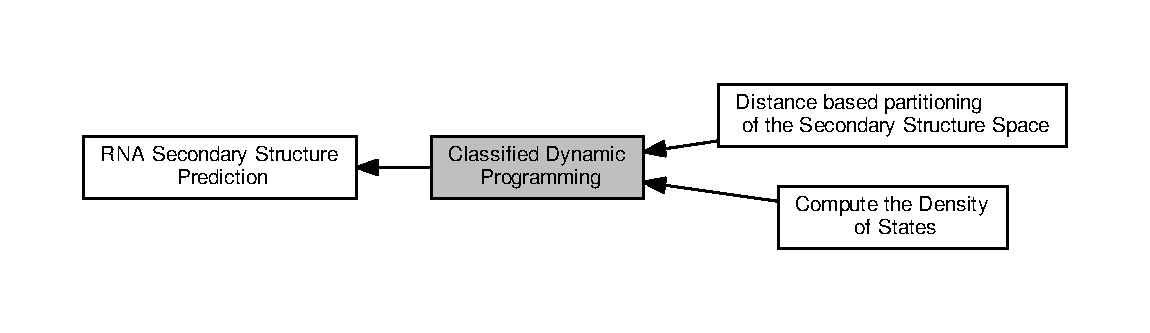
\includegraphics[width=350pt]{group__class__fold}
\end{center}
\end{figure}
\subsection*{Modules}
\begin{DoxyCompactItemize}
\item 
\hyperlink{group__kl__neighborhood}{Distance based partitioning of the Secondary Structure Space}
\begin{DoxyCompactList}\small\item\em Compute Thermodynamic properties for a Distance Class Partitioning of the Secondary Structure Space. \end{DoxyCompactList}\item 
\hyperlink{group__dos}{Compute the Density of States}
\end{DoxyCompactItemize}


\subsection{Detailed Description}

\hypertarget{group__kl__neighborhood}{}\section{Distance based partitioning of the Secondary Structure Space}
\label{group__kl__neighborhood}\index{Distance based partitioning of the Secondary Structure Space@{Distance based partitioning of the Secondary Structure Space}}


Compute Thermodynamic properties for a Distance Class Partitioning of the Secondary Structure Space.  


Collaboration diagram for Distance based partitioning of the Secondary Structure Space\+:
\nopagebreak
\begin{figure}[H]
\begin{center}
\leavevmode
\includegraphics[width=350pt]{group__kl__neighborhood}
\end{center}
\end{figure}
\subsection*{Modules}
\begin{DoxyCompactItemize}
\item 
\hyperlink{group__kl__neighborhood__mfe}{Calculating M\+F\+E representatives of a Distance Based Partitioning}
\begin{DoxyCompactList}\small\item\em Compute the minimum free energy (M\+F\+E) and secondary structures for a partitioning of the secondary structure space according to the base pair distance to two fixed reference structures basepair distance to two fixed reference structures. \end{DoxyCompactList}\item 
\hyperlink{group__kl__neighborhood__pf}{Calculate Partition Functions of a Distance Based Partitioning}
\begin{DoxyCompactList}\small\item\em Compute the partition function and stochastically sample secondary structures for a partitioning of the secondary structure space according to the base pair distance to two fixed reference structures. \end{DoxyCompactList}\item 
\hyperlink{group__kl__neighborhood__stochbt}{Stochastic Backtracking of Structures from Distance Based Partitioning}
\begin{DoxyCompactList}\small\item\em Contains functions related to stochastic backtracking from a specified distance class. \end{DoxyCompactList}\end{DoxyCompactItemize}


\subsection{Detailed Description}
Compute Thermodynamic properties for a Distance Class Partitioning of the Secondary Structure Space. 

All functions related to this group implement the basic recursions for M\+F\+E folding, partition function computation and stochastic backtracking with a {\itshape classified} {\itshape dynamic} {\itshape programming} approach. The secondary structure space is divided into partitions according to the base pair distance to two given reference structures and all relevant properties are calculated for each of the resulting partitions \begin{DoxySeeAlso}{See also}
For further details, we refer to Lorenz et al. 2009 \cite{lorenz:2009} 
\end{DoxySeeAlso}

\hypertarget{group__kl__neighborhood__mfe}{}\section{Calculating M\+F\+E representatives of a Distance Based Partitioning}
\label{group__kl__neighborhood__mfe}\index{Calculating M\+F\+E representatives of a Distance Based Partitioning@{Calculating M\+F\+E representatives of a Distance Based Partitioning}}


Compute the minimum free energy (M\+F\+E) and secondary structures for a partitioning of the secondary structure space according to the base pair distance to two fixed reference structures basepair distance to two fixed reference structures.  


Collaboration diagram for Calculating M\+F\+E representatives of a Distance Based Partitioning\+:
\nopagebreak
\begin{figure}[H]
\begin{center}
\leavevmode
\includegraphics[width=350pt]{group__kl__neighborhood__mfe}
\end{center}
\end{figure}
\subsection*{Files}
\begin{DoxyCompactItemize}
\item 
file \hyperlink{2Dfold_8h}{2\+Dfold.\+h}
\end{DoxyCompactItemize}
\subsection*{Data Structures}
\begin{DoxyCompactItemize}
\item 
struct \hyperlink{group__kl__neighborhood__mfe_structvrna__sol__TwoD__t}{vrna\+\_\+sol\+\_\+\+Two\+D\+\_\+t}
\begin{DoxyCompactList}\small\item\em Solution element returned from \hyperlink{group__kl__neighborhood__mfe_ga243c288b463147352829df04de6a2f77}{vrna\+\_\+mfe\+\_\+\+Two\+D()}  \hyperlink{group__kl__neighborhood__mfe_structvrna__sol__TwoD__t}{More...}\end{DoxyCompactList}\item 
struct \hyperlink{group__kl__neighborhood__mfe_structTwoDfold__vars}{Two\+Dfold\+\_\+vars}
\begin{DoxyCompactList}\small\item\em Variables compound for 2\+Dfold M\+F\+E folding.  \hyperlink{group__kl__neighborhood__mfe_structTwoDfold__vars}{More...}\end{DoxyCompactList}\end{DoxyCompactItemize}
\subsection*{Typedefs}
\begin{DoxyCompactItemize}
\item 
typedef struct \hyperlink{group__kl__neighborhood__mfe_structvrna__sol__TwoD__t}{vrna\+\_\+sol\+\_\+\+Two\+D\+\_\+t} \hyperlink{group__kl__neighborhood__mfe_ga6a81a58268d250309712549a3fa0aab2}{vrna\+\_\+sol\+\_\+\+Two\+D\+\_\+t}
\begin{DoxyCompactList}\small\item\em Solution element returned from \hyperlink{group__kl__neighborhood__mfe_ga243c288b463147352829df04de6a2f77}{vrna\+\_\+mfe\+\_\+\+Two\+D()} \end{DoxyCompactList}\item 
typedef struct \hyperlink{group__kl__neighborhood__mfe_structTwoDfold__vars}{Two\+Dfold\+\_\+vars} \hyperlink{group__kl__neighborhood__mfe_gaf4f514010a14f9d59d850742b3e96954}{Two\+Dfold\+\_\+vars}
\begin{DoxyCompactList}\small\item\em Variables compound for 2\+Dfold M\+F\+E folding. \end{DoxyCompactList}\end{DoxyCompactItemize}
\subsection*{Functions}
\begin{DoxyCompactItemize}
\item 
\hyperlink{group__kl__neighborhood__mfe_structvrna__sol__TwoD__t}{vrna\+\_\+sol\+\_\+\+Two\+D\+\_\+t} $\ast$ \hyperlink{group__kl__neighborhood__mfe_ga243c288b463147352829df04de6a2f77}{vrna\+\_\+mfe\+\_\+\+Two\+D} (\hyperlink{group__fold__compound_ga1b0cef17fd40466cef5968eaeeff6166}{vrna\+\_\+fold\+\_\+compound\+\_\+t} $\ast$vc, int distance1, int distance2)
\begin{DoxyCompactList}\small\item\em Compute M\+F\+E\textquotesingle{}s and representative for distance partitioning. \end{DoxyCompactList}\item 
char $\ast$ \hyperlink{group__kl__neighborhood__mfe_ga15a96fc96f4f4c2e01a11b3e17d1ef43}{vrna\+\_\+backtrack5\+\_\+\+Two\+D} (\hyperlink{group__fold__compound_ga1b0cef17fd40466cef5968eaeeff6166}{vrna\+\_\+fold\+\_\+compound\+\_\+t} $\ast$vc, int k, int l, unsigned int j)
\begin{DoxyCompactList}\small\item\em Backtrack a minimum free energy structure from a 5\textquotesingle{} section of specified length. \end{DoxyCompactList}\item 
\hyperlink{group__kl__neighborhood__mfe_structTwoDfold__vars}{Two\+Dfold\+\_\+vars} $\ast$ \hyperlink{group__kl__neighborhood__mfe_gac9284f132cf0eaa0a2f43590eda05488}{get\+\_\+\+Two\+Dfold\+\_\+variables} (const char $\ast$seq, const char $\ast$structure1, const char $\ast$structure2, int \hyperlink{group__model__details_gaf9202a1a09f5828dc731e2d9a10fa111}{circ})
\begin{DoxyCompactList}\small\item\em Get a structure of type \hyperlink{group__kl__neighborhood__mfe_structTwoDfold__vars}{Two\+Dfold\+\_\+vars} prefilled with current global settings. \end{DoxyCompactList}\item 
void \hyperlink{group__kl__neighborhood__mfe_ga05bf4f31d216b1b160fd2d3d68e9b487}{destroy\+\_\+\+Two\+Dfold\+\_\+variables} (\hyperlink{group__kl__neighborhood__mfe_structTwoDfold__vars}{Two\+Dfold\+\_\+vars} $\ast$our\+\_\+variables)
\begin{DoxyCompactList}\small\item\em Destroy a \hyperlink{group__kl__neighborhood__mfe_structTwoDfold__vars}{Two\+Dfold\+\_\+vars} datastructure without memory loss. \end{DoxyCompactList}\item 
\hyperlink{group__kl__neighborhood__mfe_structvrna__sol__TwoD__t}{vrna\+\_\+sol\+\_\+\+Two\+D\+\_\+t} $\ast$ \hyperlink{group__kl__neighborhood__mfe_ga7fc5e3e92fe97914ca4eccd33c01c2a7}{Two\+Dfold\+List} (\hyperlink{group__kl__neighborhood__mfe_structTwoDfold__vars}{Two\+Dfold\+\_\+vars} $\ast$vars, int distance1, int distance2)
\begin{DoxyCompactList}\small\item\em Compute M\+F\+E\textquotesingle{}s and representative for distance partitioning. \end{DoxyCompactList}\item 
char $\ast$ \hyperlink{group__kl__neighborhood__mfe_gaf4dc05bf8fc1ea53acd7aeb798ba80c2}{Two\+Dfold\+\_\+backtrack\+\_\+f5} (unsigned int j, int k, int l, \hyperlink{group__kl__neighborhood__mfe_structTwoDfold__vars}{Two\+Dfold\+\_\+vars} $\ast$vars)
\begin{DoxyCompactList}\small\item\em Backtrack a minimum free energy structure from a 5\textquotesingle{} section of specified length. \end{DoxyCompactList}\end{DoxyCompactItemize}


\subsection{Detailed Description}
Compute the minimum free energy (M\+F\+E) and secondary structures for a partitioning of the secondary structure space according to the base pair distance to two fixed reference structures basepair distance to two fixed reference structures. 

\begin{DoxySeeAlso}{See also}
For further details, we refer to Lorenz et al. 2009 \cite{lorenz:2009} 
\end{DoxySeeAlso}


\subsection{Data Structure Documentation}
\index{vrna\+\_\+sol\+\_\+\+Two\+D\+\_\+t@{vrna\+\_\+sol\+\_\+\+Two\+D\+\_\+t}}\label{structvrna__sol__TwoD__t}
\hypertarget{group__kl__neighborhood__mfe_structvrna__sol__TwoD__t}{}
\subsubsection{struct vrna\+\_\+sol\+\_\+\+Two\+D\+\_\+t}
Solution element returned from \hyperlink{group__kl__neighborhood__mfe_ga243c288b463147352829df04de6a2f77}{vrna\+\_\+mfe\+\_\+\+Two\+D()} 

This element contains free energy and structure for the appropriate kappa (k), lambda (l) neighborhood The datastructure contains two integer attributes \textquotesingle{}k\textquotesingle{} and \textquotesingle{}l\textquotesingle{} as well as an attribute \textquotesingle{}en\textquotesingle{} of type float representing the free energy in kcal/mol and an attribute \textquotesingle{}s\textquotesingle{} of type char$\ast$ containg the secondary structure representative,

A value of \hyperlink{energy__const_8h_a12c2040f25d8e3a7b9e1c2024c618cb6}{I\+N\+F} in k denotes the end of a list

\begin{DoxySeeAlso}{See also}
\hyperlink{group__kl__neighborhood__mfe_ga243c288b463147352829df04de6a2f77}{vrna\+\_\+mfe\+\_\+\+Two\+D()} 
\end{DoxySeeAlso}
\subsubsection*{Data Fields}
\begin{DoxyCompactItemize}
\item 
\hypertarget{group__kl__neighborhood__mfe_ac111e850bb3b3a11b6b5707912cfa1b8}{}int \hyperlink{group__kl__neighborhood__mfe_ac111e850bb3b3a11b6b5707912cfa1b8}{k}\label{group__kl__neighborhood__mfe_ac111e850bb3b3a11b6b5707912cfa1b8}

\begin{DoxyCompactList}\small\item\em Distance to first reference. \end{DoxyCompactList}\item 
\hypertarget{group__kl__neighborhood__mfe_ab8e95cd920901175a2cc8de726ab1d36}{}int \hyperlink{group__kl__neighborhood__mfe_ab8e95cd920901175a2cc8de726ab1d36}{l}\label{group__kl__neighborhood__mfe_ab8e95cd920901175a2cc8de726ab1d36}

\begin{DoxyCompactList}\small\item\em Distance to second reference. \end{DoxyCompactList}\item 
\hypertarget{group__kl__neighborhood__mfe_a7577863a6a84224dfee39b321c03cab1}{}float \hyperlink{group__kl__neighborhood__mfe_a7577863a6a84224dfee39b321c03cab1}{en}\label{group__kl__neighborhood__mfe_a7577863a6a84224dfee39b321c03cab1}

\begin{DoxyCompactList}\small\item\em Free energy in kcal/mol. \end{DoxyCompactList}\item 
\hypertarget{group__kl__neighborhood__mfe_ac5942d2505a6cd7e4a8073a321d5d2d5}{}char $\ast$ \hyperlink{group__kl__neighborhood__mfe_ac5942d2505a6cd7e4a8073a321d5d2d5}{s}\label{group__kl__neighborhood__mfe_ac5942d2505a6cd7e4a8073a321d5d2d5}

\begin{DoxyCompactList}\small\item\em M\+F\+E representative structure in dot-\/bracket notation. \end{DoxyCompactList}\end{DoxyCompactItemize}
\index{Two\+Dfold\+\_\+vars@{Two\+Dfold\+\_\+vars}}\label{structTwoDfold__vars}
\hypertarget{group__kl__neighborhood__mfe_structTwoDfold__vars}{}
\subsubsection{struct Two\+Dfold\+\_\+vars}
Variables compound for 2\+Dfold M\+F\+E folding. 

\begin{DoxyRefDesc}{Deprecated}
\item[\hyperlink{deprecated__deprecated000001}{Deprecated}]This data structure will be removed from the library soon! Use \hyperlink{group__fold__compound_ga1b0cef17fd40466cef5968eaeeff6166}{vrna\+\_\+fold\+\_\+compound\+\_\+t} and the corresponding functions vrna\+\_\+fold\+\_\+compound\+\_\+\+Two\+D(), \hyperlink{group__kl__neighborhood__mfe_ga243c288b463147352829df04de6a2f77}{vrna\+\_\+mfe\+\_\+\+Two\+D()}, and \hyperlink{group__fold__compound_gadded6039d63f5d6509836e20321534ad}{vrna\+\_\+fold\+\_\+compound\+\_\+free()} instead! \end{DoxyRefDesc}


Collaboration diagram for Two\+Dfold\+\_\+vars\+:
\nopagebreak
\begin{figure}[H]
\begin{center}
\leavevmode
\includegraphics[width=350pt]{structTwoDfold__vars__coll__graph}
\end{center}
\end{figure}
\subsubsection*{Data Fields}
\begin{DoxyCompactItemize}
\item 
\hypertarget{group__kl__neighborhood__mfe_a70da9e83ad87c37013b4bf0b265dd307}{}\hyperlink{group__energy__parameters_ga8a69ca7d787e4fd6079914f5343a1f35}{vrna\+\_\+param\+\_\+t} $\ast$ \hyperlink{group__kl__neighborhood__mfe_a70da9e83ad87c37013b4bf0b265dd307}{P}\label{group__kl__neighborhood__mfe_a70da9e83ad87c37013b4bf0b265dd307}

\begin{DoxyCompactList}\small\item\em Precomputed energy parameters and model details. \end{DoxyCompactList}\item 
\hypertarget{group__kl__neighborhood__mfe_ade5c7e9337a458ae20bac75abdc52d64}{}int \hyperlink{group__kl__neighborhood__mfe_ade5c7e9337a458ae20bac75abdc52d64}{do\+\_\+backtrack}\label{group__kl__neighborhood__mfe_ade5c7e9337a458ae20bac75abdc52d64}

\begin{DoxyCompactList}\small\item\em Flag whether to do backtracing of the structure(s) or not. \end{DoxyCompactList}\item 
\hypertarget{group__kl__neighborhood__mfe_aedf60b8b26dae05ad266d3e098d18208}{}char $\ast$ \hyperlink{group__kl__neighborhood__mfe_aedf60b8b26dae05ad266d3e098d18208}{ptype}\label{group__kl__neighborhood__mfe_aedf60b8b26dae05ad266d3e098d18208}

\begin{DoxyCompactList}\small\item\em Precomputed array of pair types. \end{DoxyCompactList}\item 
\hypertarget{group__kl__neighborhood__mfe_a3596f3d4d320318c4b8428e2abc7ab56}{}char $\ast$ \hyperlink{group__kl__neighborhood__mfe_a3596f3d4d320318c4b8428e2abc7ab56}{sequence}\label{group__kl__neighborhood__mfe_a3596f3d4d320318c4b8428e2abc7ab56}

\begin{DoxyCompactList}\small\item\em The input sequence. \end{DoxyCompactList}\item 
\hypertarget{group__kl__neighborhood__mfe_ab9ee459ffbfb5d2c138a033516056cdc}{}short $\ast$ \hyperlink{group__kl__neighborhood__mfe_ab9ee459ffbfb5d2c138a033516056cdc}{S1}\label{group__kl__neighborhood__mfe_ab9ee459ffbfb5d2c138a033516056cdc}

\begin{DoxyCompactList}\small\item\em The input sequences in numeric form. \end{DoxyCompactList}\item 
\hypertarget{group__kl__neighborhood__mfe_a621ed2ab02116f3f8f5e7120dec429eb}{}unsigned int \hyperlink{group__kl__neighborhood__mfe_a621ed2ab02116f3f8f5e7120dec429eb}{max\+D1}\label{group__kl__neighborhood__mfe_a621ed2ab02116f3f8f5e7120dec429eb}

\begin{DoxyCompactList}\small\item\em Maximum allowed base pair distance to first reference. \end{DoxyCompactList}\item 
\hypertarget{group__kl__neighborhood__mfe_a03f198a4abdb3b784486d2ba5c533aa4}{}unsigned int \hyperlink{group__kl__neighborhood__mfe_a03f198a4abdb3b784486d2ba5c533aa4}{max\+D2}\label{group__kl__neighborhood__mfe_a03f198a4abdb3b784486d2ba5c533aa4}

\begin{DoxyCompactList}\small\item\em Maximum allowed base pair distance to second reference. \end{DoxyCompactList}\item 
\hypertarget{group__kl__neighborhood__mfe_aa11f5bcd8c4fe70a91c155c877c855d5}{}unsigned int $\ast$ \hyperlink{group__kl__neighborhood__mfe_aa11f5bcd8c4fe70a91c155c877c855d5}{mm1}\label{group__kl__neighborhood__mfe_aa11f5bcd8c4fe70a91c155c877c855d5}

\begin{DoxyCompactList}\small\item\em Maximum matching matrix, reference struct 1 disallowed. \end{DoxyCompactList}\item 
\hypertarget{group__kl__neighborhood__mfe_a2eaa93316b6beb17531f0c078806036c}{}unsigned int $\ast$ \hyperlink{group__kl__neighborhood__mfe_a2eaa93316b6beb17531f0c078806036c}{mm2}\label{group__kl__neighborhood__mfe_a2eaa93316b6beb17531f0c078806036c}

\begin{DoxyCompactList}\small\item\em Maximum matching matrix, reference struct 2 disallowed. \end{DoxyCompactList}\item 
\hypertarget{group__kl__neighborhood__mfe_a1a20cb06b58b75d1a3dbdbc8bc60d0a7}{}int $\ast$ \hyperlink{group__kl__neighborhood__mfe_a1a20cb06b58b75d1a3dbdbc8bc60d0a7}{my\+\_\+iindx}\label{group__kl__neighborhood__mfe_a1a20cb06b58b75d1a3dbdbc8bc60d0a7}

\begin{DoxyCompactList}\small\item\em Index for moving in quadratic distancy dimensions. \end{DoxyCompactList}\item 
\hypertarget{group__kl__neighborhood__mfe_a536525b98c1b633d4c5f2da4f8d78c18}{}unsigned int $\ast$ \hyperlink{group__kl__neighborhood__mfe_a536525b98c1b633d4c5f2da4f8d78c18}{reference\+B\+Ps1}\label{group__kl__neighborhood__mfe_a536525b98c1b633d4c5f2da4f8d78c18}

\begin{DoxyCompactList}\small\item\em Matrix containing number of basepairs of reference structure1 in interval \mbox{[}i,j\mbox{]}. \end{DoxyCompactList}\item 
\hypertarget{group__kl__neighborhood__mfe_aa7abf73c3114cb5f0dc90e702fa9dd0f}{}unsigned int $\ast$ \hyperlink{group__kl__neighborhood__mfe_aa7abf73c3114cb5f0dc90e702fa9dd0f}{reference\+B\+Ps2}\label{group__kl__neighborhood__mfe_aa7abf73c3114cb5f0dc90e702fa9dd0f}

\begin{DoxyCompactList}\small\item\em Matrix containing number of basepairs of reference structure2 in interval \mbox{[}i,j\mbox{]}. \end{DoxyCompactList}\item 
\hypertarget{group__kl__neighborhood__mfe_af1106e1a592e2dccc92b3452340549e0}{}unsigned int $\ast$ \hyperlink{group__kl__neighborhood__mfe_af1106e1a592e2dccc92b3452340549e0}{bpdist}\label{group__kl__neighborhood__mfe_af1106e1a592e2dccc92b3452340549e0}

\begin{DoxyCompactList}\small\item\em Matrix containing base pair distance of reference structure 1 and 2 on interval \mbox{[}i,j\mbox{]}. \end{DoxyCompactList}\end{DoxyCompactItemize}


\subsection{Typedef Documentation}
\hypertarget{group__kl__neighborhood__mfe_ga6a81a58268d250309712549a3fa0aab2}{}\index{Calculating M\+F\+E representatives of a Distance Based Partitioning@{Calculating M\+F\+E representatives of a Distance Based Partitioning}!vrna\+\_\+sol\+\_\+\+Two\+D\+\_\+t@{vrna\+\_\+sol\+\_\+\+Two\+D\+\_\+t}}
\index{vrna\+\_\+sol\+\_\+\+Two\+D\+\_\+t@{vrna\+\_\+sol\+\_\+\+Two\+D\+\_\+t}!Calculating M\+F\+E representatives of a Distance Based Partitioning@{Calculating M\+F\+E representatives of a Distance Based Partitioning}}
\subsubsection[{vrna\+\_\+sol\+\_\+\+Two\+D\+\_\+t}]{\setlength{\rightskip}{0pt plus 5cm}typedef struct {\bf vrna\+\_\+sol\+\_\+\+Two\+D\+\_\+t}  {\bf vrna\+\_\+sol\+\_\+\+Two\+D\+\_\+t}}\label{group__kl__neighborhood__mfe_ga6a81a58268d250309712549a3fa0aab2}


{\ttfamily \#include $<$\hyperlink{2Dfold_8h}{Vienna\+R\+N\+A/2\+Dfold.\+h}$>$}



Solution element returned from \hyperlink{group__kl__neighborhood__mfe_ga243c288b463147352829df04de6a2f77}{vrna\+\_\+mfe\+\_\+\+Two\+D()} 

This element contains free energy and structure for the appropriate kappa (k), lambda (l) neighborhood The datastructure contains two integer attributes \textquotesingle{}k\textquotesingle{} and \textquotesingle{}l\textquotesingle{} as well as an attribute \textquotesingle{}en\textquotesingle{} of type float representing the free energy in kcal/mol and an attribute \textquotesingle{}s\textquotesingle{} of type char$\ast$ containg the secondary structure representative,

A value of \hyperlink{energy__const_8h_a12c2040f25d8e3a7b9e1c2024c618cb6}{I\+N\+F} in k denotes the end of a list

\begin{DoxySeeAlso}{See also}
\hyperlink{group__kl__neighborhood__mfe_ga243c288b463147352829df04de6a2f77}{vrna\+\_\+mfe\+\_\+\+Two\+D()} 
\end{DoxySeeAlso}
\hypertarget{group__kl__neighborhood__mfe_gaf4f514010a14f9d59d850742b3e96954}{}\index{Calculating M\+F\+E representatives of a Distance Based Partitioning@{Calculating M\+F\+E representatives of a Distance Based Partitioning}!Two\+Dfold\+\_\+vars@{Two\+Dfold\+\_\+vars}}
\index{Two\+Dfold\+\_\+vars@{Two\+Dfold\+\_\+vars}!Calculating M\+F\+E representatives of a Distance Based Partitioning@{Calculating M\+F\+E representatives of a Distance Based Partitioning}}
\subsubsection[{Two\+Dfold\+\_\+vars}]{\setlength{\rightskip}{0pt plus 5cm}typedef struct {\bf Two\+Dfold\+\_\+vars}  {\bf Two\+Dfold\+\_\+vars}}\label{group__kl__neighborhood__mfe_gaf4f514010a14f9d59d850742b3e96954}


{\ttfamily \#include $<$\hyperlink{2Dfold_8h}{Vienna\+R\+N\+A/2\+Dfold.\+h}$>$}



Variables compound for 2\+Dfold M\+F\+E folding. 

\begin{DoxyRefDesc}{Deprecated}
\item[\hyperlink{deprecated__deprecated000001}{Deprecated}]This data structure will be removed from the library soon! Use \hyperlink{group__fold__compound_ga1b0cef17fd40466cef5968eaeeff6166}{vrna\+\_\+fold\+\_\+compound\+\_\+t} and the corresponding functions vrna\+\_\+fold\+\_\+compound\+\_\+\+Two\+D(), \hyperlink{group__kl__neighborhood__mfe_ga243c288b463147352829df04de6a2f77}{vrna\+\_\+mfe\+\_\+\+Two\+D()}, and \hyperlink{group__fold__compound_gadded6039d63f5d6509836e20321534ad}{vrna\+\_\+fold\+\_\+compound\+\_\+free()} instead! \end{DoxyRefDesc}


\subsection{Function Documentation}
\hypertarget{group__kl__neighborhood__mfe_ga243c288b463147352829df04de6a2f77}{}\index{Calculating M\+F\+E representatives of a Distance Based Partitioning@{Calculating M\+F\+E representatives of a Distance Based Partitioning}!vrna\+\_\+mfe\+\_\+\+Two\+D@{vrna\+\_\+mfe\+\_\+\+Two\+D}}
\index{vrna\+\_\+mfe\+\_\+\+Two\+D@{vrna\+\_\+mfe\+\_\+\+Two\+D}!Calculating M\+F\+E representatives of a Distance Based Partitioning@{Calculating M\+F\+E representatives of a Distance Based Partitioning}}
\subsubsection[{vrna\+\_\+mfe\+\_\+\+Two\+D}]{\setlength{\rightskip}{0pt plus 5cm}{\bf vrna\+\_\+sol\+\_\+\+Two\+D\+\_\+t}$\ast$ vrna\+\_\+mfe\+\_\+\+Two\+D (
\begin{DoxyParamCaption}
\item[{{\bf vrna\+\_\+fold\+\_\+compound\+\_\+t} $\ast$}]{vc, }
\item[{int}]{distance1, }
\item[{int}]{distance2}
\end{DoxyParamCaption}
)}\label{group__kl__neighborhood__mfe_ga243c288b463147352829df04de6a2f77}


{\ttfamily \#include $<$\hyperlink{2Dfold_8h}{Vienna\+R\+N\+A/2\+Dfold.\+h}$>$}



Compute M\+F\+E\textquotesingle{}s and representative for distance partitioning. 

This function computes the minimum free energies and a representative secondary structure for each distance class according to the two references specified in the datastructure \textquotesingle{}vars\textquotesingle{}. The maximum basepair distance to each of both references may be set by the arguments \textquotesingle{}distance1\textquotesingle{} and \textquotesingle{}distance2\textquotesingle{}, respectively. If both distance arguments are set to \textquotesingle{}-\/1\textquotesingle{}, no restriction is assumed and the calculation is performed for each distance class possible.

The returned list contains an entry for each distance class. If a maximum basepair distance to either of the references was passed, an entry with k=l=-\/1 will be appended in the list, denoting the class where all structures exceeding the maximum will be thrown into. The end of the list is denoted by an attribute value of \hyperlink{energy__const_8h_a12c2040f25d8e3a7b9e1c2024c618cb6}{I\+N\+F} in the k-\/attribute of the list entry.

\begin{DoxySeeAlso}{See also}
vrna\+\_\+fold\+\_\+compound\+\_\+\+Two\+D(), \hyperlink{group__fold__compound_gadded6039d63f5d6509836e20321534ad}{vrna\+\_\+fold\+\_\+compound\+\_\+free()}, \hyperlink{group__kl__neighborhood__pf_ga0bc3427689bd09da09b8b3094a27f836}{vrna\+\_\+pf\+\_\+\+Two\+D()} \hyperlink{group__kl__neighborhood__mfe_ga15a96fc96f4f4c2e01a11b3e17d1ef43}{vrna\+\_\+backtrack5\+\_\+\+Two\+D()}, \hyperlink{group__kl__neighborhood__mfe_structvrna__sol__TwoD__t}{vrna\+\_\+sol\+\_\+\+Two\+D\+\_\+t}, \hyperlink{group__fold__compound_ga1b0cef17fd40466cef5968eaeeff6166}{vrna\+\_\+fold\+\_\+compound\+\_\+t}
\end{DoxySeeAlso}

\begin{DoxyParams}{Parameters}
{\em vc} & The datastructure containing all precomputed folding attributes \\
\hline
{\em distance1} & maximum distance to reference1 (-\/1 means no restriction) \\
\hline
{\em distance2} & maximum distance to reference2 (-\/1 means no restriction) \\
\hline
\end{DoxyParams}
\begin{DoxyReturn}{Returns}
A list of minimum free energies (and corresponding structures) for each distance class 
\end{DoxyReturn}
\hypertarget{group__kl__neighborhood__mfe_ga15a96fc96f4f4c2e01a11b3e17d1ef43}{}\index{Calculating M\+F\+E representatives of a Distance Based Partitioning@{Calculating M\+F\+E representatives of a Distance Based Partitioning}!vrna\+\_\+backtrack5\+\_\+\+Two\+D@{vrna\+\_\+backtrack5\+\_\+\+Two\+D}}
\index{vrna\+\_\+backtrack5\+\_\+\+Two\+D@{vrna\+\_\+backtrack5\+\_\+\+Two\+D}!Calculating M\+F\+E representatives of a Distance Based Partitioning@{Calculating M\+F\+E representatives of a Distance Based Partitioning}}
\subsubsection[{vrna\+\_\+backtrack5\+\_\+\+Two\+D}]{\setlength{\rightskip}{0pt plus 5cm}char$\ast$ vrna\+\_\+backtrack5\+\_\+\+Two\+D (
\begin{DoxyParamCaption}
\item[{{\bf vrna\+\_\+fold\+\_\+compound\+\_\+t} $\ast$}]{vc, }
\item[{int}]{k, }
\item[{int}]{l, }
\item[{unsigned int}]{j}
\end{DoxyParamCaption}
)}\label{group__kl__neighborhood__mfe_ga15a96fc96f4f4c2e01a11b3e17d1ef43}


{\ttfamily \#include $<$\hyperlink{2Dfold_8h}{Vienna\+R\+N\+A/2\+Dfold.\+h}$>$}



Backtrack a minimum free energy structure from a 5\textquotesingle{} section of specified length. 

This function allows to backtrack a secondary structure beginning at the 5\textquotesingle{} end, a specified length and residing in a specific distance class. If the argument \textquotesingle{}k\textquotesingle{} gets a value of -\/1, the structure that is backtracked is assumed to reside in the distance class where all structures exceeding the maximum basepair distance specified in \hyperlink{group__kl__neighborhood__mfe_ga243c288b463147352829df04de6a2f77}{vrna\+\_\+mfe\+\_\+\+Two\+D()} belong to. \begin{DoxyNote}{Note}
The argument \textquotesingle{}vars\textquotesingle{} must contain precalculated energy values in the energy matrices, i.\+e. a call to \hyperlink{group__kl__neighborhood__mfe_ga243c288b463147352829df04de6a2f77}{vrna\+\_\+mfe\+\_\+\+Two\+D()} preceding this function is mandatory!
\end{DoxyNote}
\begin{DoxySeeAlso}{See also}
\hyperlink{group__kl__neighborhood__mfe_ga243c288b463147352829df04de6a2f77}{vrna\+\_\+mfe\+\_\+\+Two\+D()}
\end{DoxySeeAlso}

\begin{DoxyParams}{Parameters}
{\em vc} & The datastructure containing all precomputed folding attributes \\
\hline
{\em j} & The length in nucleotides beginning from the 5\textquotesingle{} end \\
\hline
{\em k} & distance to reference1 (may be -\/1) \\
\hline
{\em l} & distance to reference2 \\
\hline
\end{DoxyParams}
\hypertarget{group__kl__neighborhood__mfe_gac9284f132cf0eaa0a2f43590eda05488}{}\index{Calculating M\+F\+E representatives of a Distance Based Partitioning@{Calculating M\+F\+E representatives of a Distance Based Partitioning}!get\+\_\+\+Two\+Dfold\+\_\+variables@{get\+\_\+\+Two\+Dfold\+\_\+variables}}
\index{get\+\_\+\+Two\+Dfold\+\_\+variables@{get\+\_\+\+Two\+Dfold\+\_\+variables}!Calculating M\+F\+E representatives of a Distance Based Partitioning@{Calculating M\+F\+E representatives of a Distance Based Partitioning}}
\subsubsection[{get\+\_\+\+Two\+Dfold\+\_\+variables}]{\setlength{\rightskip}{0pt plus 5cm}{\bf Two\+Dfold\+\_\+vars}$\ast$ get\+\_\+\+Two\+Dfold\+\_\+variables (
\begin{DoxyParamCaption}
\item[{const char $\ast$}]{seq, }
\item[{const char $\ast$}]{structure1, }
\item[{const char $\ast$}]{structure2, }
\item[{int}]{circ}
\end{DoxyParamCaption}
)}\label{group__kl__neighborhood__mfe_gac9284f132cf0eaa0a2f43590eda05488}


{\ttfamily \#include $<$\hyperlink{2Dfold_8h}{Vienna\+R\+N\+A/2\+Dfold.\+h}$>$}



Get a structure of type \hyperlink{group__kl__neighborhood__mfe_structTwoDfold__vars}{Two\+Dfold\+\_\+vars} prefilled with current global settings. 

This function returns a datastructure of type \hyperlink{group__kl__neighborhood__mfe_structTwoDfold__vars}{Two\+Dfold\+\_\+vars}. The data fields inside the \hyperlink{group__kl__neighborhood__mfe_structTwoDfold__vars}{Two\+Dfold\+\_\+vars} are prefilled by global settings and all memory allocations necessary to start a computation are already done for the convenience of the user

\begin{DoxyNote}{Note}
Make sure that the reference structures are compatible with the sequence according to Watson-\/\+Crick-\/ and Wobble-\/base pairing
\end{DoxyNote}
\begin{DoxyRefDesc}{Deprecated}
\item[\hyperlink{deprecated__deprecated000002}{Deprecated}]Use the new A\+P\+I that relies on \hyperlink{group__fold__compound_ga1b0cef17fd40466cef5968eaeeff6166}{vrna\+\_\+fold\+\_\+compound\+\_\+t} and the corresponding functions vrna\+\_\+fold\+\_\+compound\+\_\+\+Two\+D(), \hyperlink{group__kl__neighborhood__mfe_ga243c288b463147352829df04de6a2f77}{vrna\+\_\+mfe\+\_\+\+Two\+D()}, and \hyperlink{group__fold__compound_gadded6039d63f5d6509836e20321534ad}{vrna\+\_\+fold\+\_\+compound\+\_\+free()} instead!\end{DoxyRefDesc}



\begin{DoxyParams}{Parameters}
{\em seq} & The R\+N\+A sequence \\
\hline
{\em structure1} & The first reference structure in dot-\/bracket notation \\
\hline
{\em structure2} & The second reference structure in dot-\/bracket notation \\
\hline
{\em circ} & A switch to indicate the assumption to fold a circular instead of linear R\+N\+A (0=O\+F\+F, 1=O\+N) \\
\hline
\end{DoxyParams}
\begin{DoxyReturn}{Returns}
A datastructure prefilled with folding options and allocated memory 
\end{DoxyReturn}
\hypertarget{group__kl__neighborhood__mfe_ga05bf4f31d216b1b160fd2d3d68e9b487}{}\index{Calculating M\+F\+E representatives of a Distance Based Partitioning@{Calculating M\+F\+E representatives of a Distance Based Partitioning}!destroy\+\_\+\+Two\+Dfold\+\_\+variables@{destroy\+\_\+\+Two\+Dfold\+\_\+variables}}
\index{destroy\+\_\+\+Two\+Dfold\+\_\+variables@{destroy\+\_\+\+Two\+Dfold\+\_\+variables}!Calculating M\+F\+E representatives of a Distance Based Partitioning@{Calculating M\+F\+E representatives of a Distance Based Partitioning}}
\subsubsection[{destroy\+\_\+\+Two\+Dfold\+\_\+variables}]{\setlength{\rightskip}{0pt plus 5cm}void destroy\+\_\+\+Two\+Dfold\+\_\+variables (
\begin{DoxyParamCaption}
\item[{{\bf Two\+Dfold\+\_\+vars} $\ast$}]{our\+\_\+variables}
\end{DoxyParamCaption}
)}\label{group__kl__neighborhood__mfe_ga05bf4f31d216b1b160fd2d3d68e9b487}


{\ttfamily \#include $<$\hyperlink{2Dfold_8h}{Vienna\+R\+N\+A/2\+Dfold.\+h}$>$}



Destroy a \hyperlink{group__kl__neighborhood__mfe_structTwoDfold__vars}{Two\+Dfold\+\_\+vars} datastructure without memory loss. 

This function free\textquotesingle{}s all allocated memory that depends on the datastructure given.

\begin{DoxyRefDesc}{Deprecated}
\item[\hyperlink{deprecated__deprecated000003}{Deprecated}]Use the new A\+P\+I that relies on \hyperlink{group__fold__compound_ga1b0cef17fd40466cef5968eaeeff6166}{vrna\+\_\+fold\+\_\+compound\+\_\+t} and the corresponding functions vrna\+\_\+fold\+\_\+compound\+\_\+\+Two\+D(), \hyperlink{group__kl__neighborhood__mfe_ga243c288b463147352829df04de6a2f77}{vrna\+\_\+mfe\+\_\+\+Two\+D()}, and \hyperlink{group__fold__compound_gadded6039d63f5d6509836e20321534ad}{vrna\+\_\+fold\+\_\+compound\+\_\+free()} instead!\end{DoxyRefDesc}



\begin{DoxyParams}{Parameters}
{\em our\+\_\+variables} & A pointer to the datastructure to be destroyed \\
\hline
\end{DoxyParams}
\hypertarget{group__kl__neighborhood__mfe_ga7fc5e3e92fe97914ca4eccd33c01c2a7}{}\index{Calculating M\+F\+E representatives of a Distance Based Partitioning@{Calculating M\+F\+E representatives of a Distance Based Partitioning}!Two\+Dfold\+List@{Two\+Dfold\+List}}
\index{Two\+Dfold\+List@{Two\+Dfold\+List}!Calculating M\+F\+E representatives of a Distance Based Partitioning@{Calculating M\+F\+E representatives of a Distance Based Partitioning}}
\subsubsection[{Two\+Dfold\+List}]{\setlength{\rightskip}{0pt plus 5cm}{\bf vrna\+\_\+sol\+\_\+\+Two\+D\+\_\+t}$\ast$ Two\+Dfold\+List (
\begin{DoxyParamCaption}
\item[{{\bf Two\+Dfold\+\_\+vars} $\ast$}]{vars, }
\item[{int}]{distance1, }
\item[{int}]{distance2}
\end{DoxyParamCaption}
)}\label{group__kl__neighborhood__mfe_ga7fc5e3e92fe97914ca4eccd33c01c2a7}


{\ttfamily \#include $<$\hyperlink{2Dfold_8h}{Vienna\+R\+N\+A/2\+Dfold.\+h}$>$}



Compute M\+F\+E\textquotesingle{}s and representative for distance partitioning. 

This function computes the minimum free energies and a representative secondary structure for each distance class according to the two references specified in the datastructure \textquotesingle{}vars\textquotesingle{}. The maximum basepair distance to each of both references may be set by the arguments \textquotesingle{}distance1\textquotesingle{} and \textquotesingle{}distance2\textquotesingle{}, respectively. If both distance arguments are set to \textquotesingle{}-\/1\textquotesingle{}, no restriction is assumed and the calculation is performed for each distance class possible.

The returned list contains an entry for each distance class. If a maximum basepair distance to either of the references was passed, an entry with k=l=-\/1 will be appended in the list, denoting the class where all structures exceeding the maximum will be thrown into. The end of the list is denoted by an attribute value of \hyperlink{energy__const_8h_a12c2040f25d8e3a7b9e1c2024c618cb6}{I\+N\+F} in the k-\/attribute of the list entry.

\begin{DoxyRefDesc}{Deprecated}
\item[\hyperlink{deprecated__deprecated000004}{Deprecated}]Use the new A\+P\+I that relies on \hyperlink{group__fold__compound_ga1b0cef17fd40466cef5968eaeeff6166}{vrna\+\_\+fold\+\_\+compound\+\_\+t} and the corresponding functions vrna\+\_\+fold\+\_\+compound\+\_\+\+Two\+D(), \hyperlink{group__kl__neighborhood__mfe_ga243c288b463147352829df04de6a2f77}{vrna\+\_\+mfe\+\_\+\+Two\+D()}, and \hyperlink{group__fold__compound_gadded6039d63f5d6509836e20321534ad}{vrna\+\_\+fold\+\_\+compound\+\_\+free()} instead!\end{DoxyRefDesc}



\begin{DoxyParams}{Parameters}
{\em vars} & the datastructure containing all predefined folding attributes \\
\hline
{\em distance1} & maximum distance to reference1 (-\/1 means no restriction) \\
\hline
{\em distance2} & maximum distance to reference2 (-\/1 means no restriction) \\
\hline
\end{DoxyParams}
\hypertarget{group__kl__neighborhood__mfe_gaf4dc05bf8fc1ea53acd7aeb798ba80c2}{}\index{Calculating M\+F\+E representatives of a Distance Based Partitioning@{Calculating M\+F\+E representatives of a Distance Based Partitioning}!Two\+Dfold\+\_\+backtrack\+\_\+f5@{Two\+Dfold\+\_\+backtrack\+\_\+f5}}
\index{Two\+Dfold\+\_\+backtrack\+\_\+f5@{Two\+Dfold\+\_\+backtrack\+\_\+f5}!Calculating M\+F\+E representatives of a Distance Based Partitioning@{Calculating M\+F\+E representatives of a Distance Based Partitioning}}
\subsubsection[{Two\+Dfold\+\_\+backtrack\+\_\+f5}]{\setlength{\rightskip}{0pt plus 5cm}char$\ast$ Two\+Dfold\+\_\+backtrack\+\_\+f5 (
\begin{DoxyParamCaption}
\item[{unsigned int}]{j, }
\item[{int}]{k, }
\item[{int}]{l, }
\item[{{\bf Two\+Dfold\+\_\+vars} $\ast$}]{vars}
\end{DoxyParamCaption}
)}\label{group__kl__neighborhood__mfe_gaf4dc05bf8fc1ea53acd7aeb798ba80c2}


{\ttfamily \#include $<$\hyperlink{2Dfold_8h}{Vienna\+R\+N\+A/2\+Dfold.\+h}$>$}



Backtrack a minimum free energy structure from a 5\textquotesingle{} section of specified length. 

This function allows to backtrack a secondary structure beginning at the 5\textquotesingle{} end, a specified length and residing in a specific distance class. If the argument \textquotesingle{}k\textquotesingle{} gets a value of -\/1, the structure that is backtracked is assumed to reside in the distance class where all structures exceeding the maximum basepair distance specified in Two\+Dfold() belong to. \begin{DoxyNote}{Note}
The argument \textquotesingle{}vars\textquotesingle{} must contain precalculated energy values in the energy matrices, i.\+e. a call to Two\+Dfold() preceding this function is mandatory!
\end{DoxyNote}
\begin{DoxyRefDesc}{Deprecated}
\item[\hyperlink{deprecated__deprecated000005}{Deprecated}]Use the new A\+P\+I that relies on \hyperlink{group__fold__compound_ga1b0cef17fd40466cef5968eaeeff6166}{vrna\+\_\+fold\+\_\+compound\+\_\+t} and the corresponding functions vrna\+\_\+fold\+\_\+compound\+\_\+\+Two\+D(), \hyperlink{group__kl__neighborhood__mfe_ga243c288b463147352829df04de6a2f77}{vrna\+\_\+mfe\+\_\+\+Two\+D()}, \hyperlink{group__kl__neighborhood__mfe_ga15a96fc96f4f4c2e01a11b3e17d1ef43}{vrna\+\_\+backtrack5\+\_\+\+Two\+D()}, and \hyperlink{group__fold__compound_gadded6039d63f5d6509836e20321534ad}{vrna\+\_\+fold\+\_\+compound\+\_\+free()} instead!\end{DoxyRefDesc}



\begin{DoxyParams}{Parameters}
{\em j} & The length in nucleotides beginning from the 5\textquotesingle{} end \\
\hline
{\em k} & distance to reference1 (may be -\/1) \\
\hline
{\em l} & distance to reference2 \\
\hline
{\em vars} & the datastructure containing all predefined folding attributes \\
\hline
\end{DoxyParams}

\hypertarget{group__kl__neighborhood__pf}{}\section{Calculate Partition Functions of a Distance Based Partitioning}
\label{group__kl__neighborhood__pf}\index{Calculate Partition Functions of a Distance Based Partitioning@{Calculate Partition Functions of a Distance Based Partitioning}}


Compute the partition function and stochastically sample secondary structures for a partitioning of the secondary structure space according to the base pair distance to two fixed reference structures.  


Collaboration diagram for Calculate Partition Functions of a Distance Based Partitioning\+:
\nopagebreak
\begin{figure}[H]
\begin{center}
\leavevmode
\includegraphics[width=350pt]{group__kl__neighborhood__pf}
\end{center}
\end{figure}
\subsection*{Files}
\begin{DoxyCompactItemize}
\item 
file \hyperlink{2Dpfold_8h}{2\+Dpfold.\+h}
\end{DoxyCompactItemize}
\subsection*{Data Structures}
\begin{DoxyCompactItemize}
\item 
struct \hyperlink{group__kl__neighborhood__pf_structvrna__sol__TwoD__pf__t}{vrna\+\_\+sol\+\_\+\+Two\+D\+\_\+pf\+\_\+t}
\begin{DoxyCompactList}\small\item\em Solution element returned from \hyperlink{group__kl__neighborhood__pf_ga0bc3427689bd09da09b8b3094a27f836}{vrna\+\_\+pf\+\_\+\+Two\+D()}  \hyperlink{group__kl__neighborhood__pf_structvrna__sol__TwoD__pf__t}{More...}\end{DoxyCompactList}\end{DoxyCompactItemize}
\subsection*{Typedefs}
\begin{DoxyCompactItemize}
\item 
typedef struct \hyperlink{group__kl__neighborhood__pf_structvrna__sol__TwoD__pf__t}{vrna\+\_\+sol\+\_\+\+Two\+D\+\_\+pf\+\_\+t} \hyperlink{group__kl__neighborhood__pf_ga5e449fbd695406aabd2bcabddc374621}{vrna\+\_\+sol\+\_\+\+Two\+D\+\_\+pf\+\_\+t}
\begin{DoxyCompactList}\small\item\em Solution element returned from \hyperlink{group__kl__neighborhood__pf_ga0bc3427689bd09da09b8b3094a27f836}{vrna\+\_\+pf\+\_\+\+Two\+D()} \end{DoxyCompactList}\end{DoxyCompactItemize}
\subsection*{Functions}
\begin{DoxyCompactItemize}
\item 
\hyperlink{group__kl__neighborhood__pf_structvrna__sol__TwoD__pf__t}{vrna\+\_\+sol\+\_\+\+Two\+D\+\_\+pf\+\_\+t} $\ast$ \hyperlink{group__kl__neighborhood__pf_ga0bc3427689bd09da09b8b3094a27f836}{vrna\+\_\+pf\+\_\+\+Two\+D} (\hyperlink{group__fold__compound_ga1b0cef17fd40466cef5968eaeeff6166}{vrna\+\_\+fold\+\_\+compound\+\_\+t} $\ast$vc, int max\+Distance1, int max\+Distance2)
\begin{DoxyCompactList}\small\item\em Compute the partition function for all distance classes. \end{DoxyCompactList}\end{DoxyCompactItemize}


\subsection{Detailed Description}
Compute the partition function and stochastically sample secondary structures for a partitioning of the secondary structure space according to the base pair distance to two fixed reference structures. 



\subsection{Data Structure Documentation}
\index{vrna\+\_\+sol\+\_\+\+Two\+D\+\_\+pf\+\_\+t@{vrna\+\_\+sol\+\_\+\+Two\+D\+\_\+pf\+\_\+t}}\label{structvrna__sol__TwoD__pf__t}
\hypertarget{group__kl__neighborhood__pf_structvrna__sol__TwoD__pf__t}{}
\subsubsection{struct vrna\+\_\+sol\+\_\+\+Two\+D\+\_\+pf\+\_\+t}
Solution element returned from \hyperlink{group__kl__neighborhood__pf_ga0bc3427689bd09da09b8b3094a27f836}{vrna\+\_\+pf\+\_\+\+Two\+D()} 

This element contains the partition function for the appropriate kappa (k), lambda (l) neighborhood The datastructure contains two integer attributes \textquotesingle{}k\textquotesingle{} and \textquotesingle{}l\textquotesingle{} as well as an attribute \textquotesingle{}q\textquotesingle{} of type \hyperlink{group__data__structures_ga31125aeace516926bf7f251f759b6126}{F\+L\+T\+\_\+\+O\+R\+\_\+\+D\+B\+L}

A value of \hyperlink{energy__const_8h_a12c2040f25d8e3a7b9e1c2024c618cb6}{I\+N\+F} in k denotes the end of a list

\begin{DoxySeeAlso}{See also}
\hyperlink{group__kl__neighborhood__pf_ga0bc3427689bd09da09b8b3094a27f836}{vrna\+\_\+pf\+\_\+\+Two\+D()} 
\end{DoxySeeAlso}
\subsubsection*{Data Fields}
\begin{DoxyCompactItemize}
\item 
\hypertarget{group__kl__neighborhood__pf_ad1f23b46dc4ebd373abdeb0382d87b83}{}int \hyperlink{group__kl__neighborhood__pf_ad1f23b46dc4ebd373abdeb0382d87b83}{k}\label{group__kl__neighborhood__pf_ad1f23b46dc4ebd373abdeb0382d87b83}

\begin{DoxyCompactList}\small\item\em Distance to first reference. \end{DoxyCompactList}\item 
\hypertarget{group__kl__neighborhood__pf_a01133c264eff2c988d144e07803d1b8b}{}int \hyperlink{group__kl__neighborhood__pf_a01133c264eff2c988d144e07803d1b8b}{l}\label{group__kl__neighborhood__pf_a01133c264eff2c988d144e07803d1b8b}

\begin{DoxyCompactList}\small\item\em Distance to second reference. \end{DoxyCompactList}\item 
\hypertarget{group__kl__neighborhood__pf_a17ebbf425b8769ded74b5c7b85e58ee1}{}\hyperlink{group__data__structures_ga31125aeace516926bf7f251f759b6126}{F\+L\+T\+\_\+\+O\+R\+\_\+\+D\+B\+L} \hyperlink{group__kl__neighborhood__pf_a17ebbf425b8769ded74b5c7b85e58ee1}{q}\label{group__kl__neighborhood__pf_a17ebbf425b8769ded74b5c7b85e58ee1}

\begin{DoxyCompactList}\small\item\em partition function \end{DoxyCompactList}\end{DoxyCompactItemize}


\subsection{Typedef Documentation}
\hypertarget{group__kl__neighborhood__pf_ga5e449fbd695406aabd2bcabddc374621}{}\index{Calculate Partition Functions of a Distance Based Partitioning@{Calculate Partition Functions of a Distance Based Partitioning}!vrna\+\_\+sol\+\_\+\+Two\+D\+\_\+pf\+\_\+t@{vrna\+\_\+sol\+\_\+\+Two\+D\+\_\+pf\+\_\+t}}
\index{vrna\+\_\+sol\+\_\+\+Two\+D\+\_\+pf\+\_\+t@{vrna\+\_\+sol\+\_\+\+Two\+D\+\_\+pf\+\_\+t}!Calculate Partition Functions of a Distance Based Partitioning@{Calculate Partition Functions of a Distance Based Partitioning}}
\subsubsection[{vrna\+\_\+sol\+\_\+\+Two\+D\+\_\+pf\+\_\+t}]{\setlength{\rightskip}{0pt plus 5cm}typedef struct {\bf vrna\+\_\+sol\+\_\+\+Two\+D\+\_\+pf\+\_\+t}  {\bf vrna\+\_\+sol\+\_\+\+Two\+D\+\_\+pf\+\_\+t}}\label{group__kl__neighborhood__pf_ga5e449fbd695406aabd2bcabddc374621}


{\ttfamily \#include $<$\hyperlink{2Dpfold_8h}{Vienna\+R\+N\+A/2\+Dpfold.\+h}$>$}



Solution element returned from \hyperlink{group__kl__neighborhood__pf_ga0bc3427689bd09da09b8b3094a27f836}{vrna\+\_\+pf\+\_\+\+Two\+D()} 

This element contains the partition function for the appropriate kappa (k), lambda (l) neighborhood The datastructure contains two integer attributes \textquotesingle{}k\textquotesingle{} and \textquotesingle{}l\textquotesingle{} as well as an attribute \textquotesingle{}q\textquotesingle{} of type \hyperlink{group__data__structures_ga31125aeace516926bf7f251f759b6126}{F\+L\+T\+\_\+\+O\+R\+\_\+\+D\+B\+L}

A value of \hyperlink{energy__const_8h_a12c2040f25d8e3a7b9e1c2024c618cb6}{I\+N\+F} in k denotes the end of a list

\begin{DoxySeeAlso}{See also}
\hyperlink{group__kl__neighborhood__pf_ga0bc3427689bd09da09b8b3094a27f836}{vrna\+\_\+pf\+\_\+\+Two\+D()} 
\end{DoxySeeAlso}


\subsection{Function Documentation}
\hypertarget{group__kl__neighborhood__pf_ga0bc3427689bd09da09b8b3094a27f836}{}\index{Calculate Partition Functions of a Distance Based Partitioning@{Calculate Partition Functions of a Distance Based Partitioning}!vrna\+\_\+pf\+\_\+\+Two\+D@{vrna\+\_\+pf\+\_\+\+Two\+D}}
\index{vrna\+\_\+pf\+\_\+\+Two\+D@{vrna\+\_\+pf\+\_\+\+Two\+D}!Calculate Partition Functions of a Distance Based Partitioning@{Calculate Partition Functions of a Distance Based Partitioning}}
\subsubsection[{vrna\+\_\+pf\+\_\+\+Two\+D}]{\setlength{\rightskip}{0pt plus 5cm}{\bf vrna\+\_\+sol\+\_\+\+Two\+D\+\_\+pf\+\_\+t}$\ast$ vrna\+\_\+pf\+\_\+\+Two\+D (
\begin{DoxyParamCaption}
\item[{{\bf vrna\+\_\+fold\+\_\+compound\+\_\+t} $\ast$}]{vc, }
\item[{int}]{max\+Distance1, }
\item[{int}]{max\+Distance2}
\end{DoxyParamCaption}
)}\label{group__kl__neighborhood__pf_ga0bc3427689bd09da09b8b3094a27f836}


{\ttfamily \#include $<$\hyperlink{2Dpfold_8h}{Vienna\+R\+N\+A/2\+Dpfold.\+h}$>$}



Compute the partition function for all distance classes. 

This function computes the partition functions for all distance classes according the two reference structures specified in the datastructure \textquotesingle{}vars\textquotesingle{}. Similar to \hyperlink{group__kl__neighborhood__mfe_ga243c288b463147352829df04de6a2f77}{vrna\+\_\+mfe\+\_\+\+Two\+D()} the arguments max\+Distance1 and max\+Distance2 specify the maximum distance to both reference structures. A value of \textquotesingle{}-\/1\textquotesingle{} in either of them makes the appropriate distance restrictionless, i.\+e. all basepair distancies to the reference are taken into account during computation. In case there is a restriction, the returned solution contains an entry where the attribute k=l=-\/1 contains the partition function for all structures exceeding the restriction. A value of \hyperlink{energy__const_8h_a12c2040f25d8e3a7b9e1c2024c618cb6}{I\+N\+F} in the attribute \textquotesingle{}k\textquotesingle{} of the returned list denotes the end of the list

\begin{DoxySeeAlso}{See also}
vrna\+\_\+fold\+\_\+compound\+\_\+\+Two\+D(), \hyperlink{group__fold__compound_gadded6039d63f5d6509836e20321534ad}{vrna\+\_\+fold\+\_\+compound\+\_\+free()}, \hyperlink{group__fold__compound_ga6601d994ba32b11511b36f68b08403be}{vrna\+\_\+fold\+\_\+compound} \hyperlink{group__kl__neighborhood__pf_structvrna__sol__TwoD__pf__t}{vrna\+\_\+sol\+\_\+\+Two\+D\+\_\+pf\+\_\+t}
\end{DoxySeeAlso}

\begin{DoxyParams}{Parameters}
{\em vc} & The datastructure containing all necessary folding attributes and matrices \\
\hline
{\em max\+Distance1} & The maximum basepair distance to reference1 (may be -\/1) \\
\hline
{\em max\+Distance2} & The maximum basepair distance to reference2 (may be -\/1) \\
\hline
\end{DoxyParams}
\begin{DoxyReturn}{Returns}
A list of partition funtions for the corresponding distance classes 
\end{DoxyReturn}

\hypertarget{group__kl__neighborhood__stochbt}{}\section{Stochastic Backtracking of Structures from Distance Based Partitioning}
\label{group__kl__neighborhood__stochbt}\index{Stochastic Backtracking of Structures from Distance Based Partitioning@{Stochastic Backtracking of Structures from Distance Based Partitioning}}


Contains functions related to stochastic backtracking from a specified distance class.  


Collaboration diagram for Stochastic Backtracking of Structures from Distance Based Partitioning\+:
\nopagebreak
\begin{figure}[H]
\begin{center}
\leavevmode
\includegraphics[width=350pt]{group__kl__neighborhood__stochbt}
\end{center}
\end{figure}
\subsection*{Functions}
\begin{DoxyCompactItemize}
\item 
char $\ast$ \hyperlink{group__kl__neighborhood__stochbt_ga14aceef73f83bbde77bb3a0ca06c9d13}{vrna\+\_\+pbacktrack\+\_\+\+Two\+D} (\hyperlink{group__fold__compound_ga1b0cef17fd40466cef5968eaeeff6166}{vrna\+\_\+fold\+\_\+compound\+\_\+t} $\ast$vc, int d1, int d2)
\begin{DoxyCompactList}\small\item\em Sample secondary structure representatives from a set of distance classes according to their Boltzmann probability. \end{DoxyCompactList}\item 
char $\ast$ \hyperlink{group__kl__neighborhood__stochbt_ga6504913303bc325659c365d5f59b41e0}{vrna\+\_\+pbacktrack5\+\_\+\+Two\+D} (\hyperlink{group__fold__compound_ga1b0cef17fd40466cef5968eaeeff6166}{vrna\+\_\+fold\+\_\+compound\+\_\+t} $\ast$vc, int d1, int d2, unsigned int length)
\begin{DoxyCompactList}\small\item\em Sample secondary structure representatives with a specified length from a set of distance classes according to their Boltzmann probability. \end{DoxyCompactList}\end{DoxyCompactItemize}


\subsection{Detailed Description}
Contains functions related to stochastic backtracking from a specified distance class. 



\subsection{Function Documentation}
\hypertarget{group__kl__neighborhood__stochbt_ga14aceef73f83bbde77bb3a0ca06c9d13}{}\index{Stochastic Backtracking of Structures from Distance Based Partitioning@{Stochastic Backtracking of Structures from Distance Based Partitioning}!vrna\+\_\+pbacktrack\+\_\+\+Two\+D@{vrna\+\_\+pbacktrack\+\_\+\+Two\+D}}
\index{vrna\+\_\+pbacktrack\+\_\+\+Two\+D@{vrna\+\_\+pbacktrack\+\_\+\+Two\+D}!Stochastic Backtracking of Structures from Distance Based Partitioning@{Stochastic Backtracking of Structures from Distance Based Partitioning}}
\subsubsection[{vrna\+\_\+pbacktrack\+\_\+\+Two\+D}]{\setlength{\rightskip}{0pt plus 5cm}char$\ast$ vrna\+\_\+pbacktrack\+\_\+\+Two\+D (
\begin{DoxyParamCaption}
\item[{{\bf vrna\+\_\+fold\+\_\+compound\+\_\+t} $\ast$}]{vc, }
\item[{int}]{d1, }
\item[{int}]{d2}
\end{DoxyParamCaption}
)}\label{group__kl__neighborhood__stochbt_ga14aceef73f83bbde77bb3a0ca06c9d13}


{\ttfamily \#include $<$\hyperlink{2Dpfold_8h}{Vienna\+R\+N\+A/2\+Dpfold.\+h}$>$}



Sample secondary structure representatives from a set of distance classes according to their Boltzmann probability. 

If the argument \textquotesingle{}d1\textquotesingle{} is set to \textquotesingle{}-\/1\textquotesingle{}, the structure will be backtracked in the distance class where all structures exceeding the maximum basepair distance to either of the references reside.

\begin{DoxyPrecond}{Precondition}
The argument \textquotesingle{}vars\textquotesingle{} must contain precalculated partition function matrices, i.\+e. a call to \hyperlink{group__kl__neighborhood__pf_ga0bc3427689bd09da09b8b3094a27f836}{vrna\+\_\+pf\+\_\+\+Two\+D()} preceding this function is mandatory!
\end{DoxyPrecond}
\begin{DoxySeeAlso}{See also}
\hyperlink{group__kl__neighborhood__pf_ga0bc3427689bd09da09b8b3094a27f836}{vrna\+\_\+pf\+\_\+\+Two\+D()}
\end{DoxySeeAlso}

\begin{DoxyParams}[1]{Parameters}
\mbox{\tt in}  & {\em vars} & the datastructure containing all necessary folding attributes and matrices \\
\hline
\mbox{\tt in}  & {\em d1} & the distance to reference1 (may be -\/1) \\
\hline
\mbox{\tt in}  & {\em d2} & the distance to reference2 \\
\hline
\end{DoxyParams}
\begin{DoxyReturn}{Returns}
A sampled secondary structure in dot-\/bracket notation 
\end{DoxyReturn}
\hypertarget{group__kl__neighborhood__stochbt_ga6504913303bc325659c365d5f59b41e0}{}\index{Stochastic Backtracking of Structures from Distance Based Partitioning@{Stochastic Backtracking of Structures from Distance Based Partitioning}!vrna\+\_\+pbacktrack5\+\_\+\+Two\+D@{vrna\+\_\+pbacktrack5\+\_\+\+Two\+D}}
\index{vrna\+\_\+pbacktrack5\+\_\+\+Two\+D@{vrna\+\_\+pbacktrack5\+\_\+\+Two\+D}!Stochastic Backtracking of Structures from Distance Based Partitioning@{Stochastic Backtracking of Structures from Distance Based Partitioning}}
\subsubsection[{vrna\+\_\+pbacktrack5\+\_\+\+Two\+D}]{\setlength{\rightskip}{0pt plus 5cm}char$\ast$ vrna\+\_\+pbacktrack5\+\_\+\+Two\+D (
\begin{DoxyParamCaption}
\item[{{\bf vrna\+\_\+fold\+\_\+compound\+\_\+t} $\ast$}]{vc, }
\item[{int}]{d1, }
\item[{int}]{d2, }
\item[{unsigned int}]{length}
\end{DoxyParamCaption}
)}\label{group__kl__neighborhood__stochbt_ga6504913303bc325659c365d5f59b41e0}


{\ttfamily \#include $<$\hyperlink{2Dpfold_8h}{Vienna\+R\+N\+A/2\+Dpfold.\+h}$>$}



Sample secondary structure representatives with a specified length from a set of distance classes according to their Boltzmann probability. 

This function does essentially the same as \hyperlink{group__kl__neighborhood__stochbt_ga14aceef73f83bbde77bb3a0ca06c9d13}{vrna\+\_\+pbacktrack\+\_\+\+Two\+D()} with the only difference that partial structures, i.\+e. structures beginning from the 5\textquotesingle{} end with a specified length of the sequence, are backtracked

\begin{DoxyNote}{Note}
This function does not work (since it makes no sense) for circular R\+N\+A sequences! 
\end{DoxyNote}
\begin{DoxyPrecond}{Precondition}
The argument \textquotesingle{}vars\textquotesingle{} must contain precalculated partition function matrices, i.\+e. a call to \hyperlink{group__kl__neighborhood__pf_ga0bc3427689bd09da09b8b3094a27f836}{vrna\+\_\+pf\+\_\+\+Two\+D()} preceding this function is mandatory!
\end{DoxyPrecond}
\begin{DoxySeeAlso}{See also}
\hyperlink{group__kl__neighborhood__stochbt_ga14aceef73f83bbde77bb3a0ca06c9d13}{vrna\+\_\+pbacktrack\+\_\+\+Two\+D()}, \hyperlink{group__kl__neighborhood__pf_ga0bc3427689bd09da09b8b3094a27f836}{vrna\+\_\+pf\+\_\+\+Two\+D()}
\end{DoxySeeAlso}

\begin{DoxyParams}[1]{Parameters}
\mbox{\tt in}  & {\em vars} & the datastructure containing all necessary folding attributes and matrices \\
\hline
\mbox{\tt in}  & {\em d1} & the distance to reference1 (may be -\/1) \\
\hline
\mbox{\tt in}  & {\em d2} & the distance to reference2 \\
\hline
\mbox{\tt in}  & {\em length} & the length of the structure beginning from the 5\textquotesingle{} end \\
\hline
\end{DoxyParams}
\begin{DoxyReturn}{Returns}
A sampled secondary structure in dot-\/bracket notation 
\end{DoxyReturn}

\hypertarget{group__dos}{}\section{Compute the Density of States}
\label{group__dos}\index{Compute the Density of States@{Compute the Density of States}}
Collaboration diagram for Compute the Density of States\+:
\nopagebreak
\begin{figure}[H]
\begin{center}
\leavevmode
\includegraphics[width=328pt]{group__dos}
\end{center}
\end{figure}
\subsection*{Variables}
\begin{DoxyCompactItemize}
\item 
int \hyperlink{group__dos_ga937634a76b46a22530a74906f1957a9e}{density\+\_\+of\+\_\+states} \mbox{[}\hyperlink{subopt_8h_a5ec740b80afb4906ba4311dbd8ddbd89}{M\+A\+X\+D\+O\+S}+1\mbox{]}
\begin{DoxyCompactList}\small\item\em The Density of States. \end{DoxyCompactList}\end{DoxyCompactItemize}


\subsection{Detailed Description}


\subsection{Variable Documentation}
\hypertarget{group__dos_ga937634a76b46a22530a74906f1957a9e}{}\index{Compute the Density of States@{Compute the Density of States}!density\+\_\+of\+\_\+states@{density\+\_\+of\+\_\+states}}
\index{density\+\_\+of\+\_\+states@{density\+\_\+of\+\_\+states}!Compute the Density of States@{Compute the Density of States}}
\subsubsection[{density\+\_\+of\+\_\+states}]{\setlength{\rightskip}{0pt plus 5cm}int density\+\_\+of\+\_\+states\mbox{[}{\bf M\+A\+X\+D\+O\+S}+1\mbox{]}}\label{group__dos_ga937634a76b46a22530a74906f1957a9e}


{\ttfamily \#include $<$\hyperlink{subopt_8h}{Vienna\+R\+N\+A/subopt.\+h}$>$}



The Density of States. 

This array contains the density of states for an R\+N\+A sequences after a call to \hyperlink{group__subopt__wuchty_gaa1e1e7031a948ebcb39a9d58d1e9842c}{subopt\+\_\+par()}, \hyperlink{group__subopt__wuchty_ga700f662506a233e42dd7fda74fafd40e}{subopt()} or \hyperlink{group__subopt__wuchty_ga8634516e4740e0b6c9a46d2bae940340}{subopt\+\_\+circ()}.

\begin{DoxyPrecond}{Precondition}
Call one of the functions \hyperlink{group__subopt__wuchty_gaa1e1e7031a948ebcb39a9d58d1e9842c}{subopt\+\_\+par()}, \hyperlink{group__subopt__wuchty_ga700f662506a233e42dd7fda74fafd40e}{subopt()} or \hyperlink{group__subopt__wuchty_ga8634516e4740e0b6c9a46d2bae940340}{subopt\+\_\+circ()} prior accessing the contents of this array 
\end{DoxyPrecond}
\begin{DoxySeeAlso}{See also}
\hyperlink{group__subopt__wuchty_gaa1e1e7031a948ebcb39a9d58d1e9842c}{subopt\+\_\+par()}, \hyperlink{group__subopt__wuchty_ga700f662506a233e42dd7fda74fafd40e}{subopt()}, \hyperlink{group__subopt__wuchty_ga8634516e4740e0b6c9a46d2bae940340}{subopt\+\_\+circ()} 
\end{DoxySeeAlso}

\hypertarget{group__hard__constraints}{}\section{Hard Constraints}
\label{group__hard__constraints}\index{Hard Constraints@{Hard Constraints}}


This module covers all functionality for hard constraints in secondary structure prediction.  


Collaboration diagram for Hard Constraints\+:
\nopagebreak
\begin{figure}[H]
\begin{center}
\leavevmode
\includegraphics[width=344pt]{group__hard__constraints}
\end{center}
\end{figure}
\subsection*{Files}
\begin{DoxyCompactItemize}
\item 
file \hyperlink{constraints__hard_8h}{constraints\+\_\+hard.\+h}
\begin{DoxyCompactList}\small\item\em Functions and data structures for handling of secondary structure hard constraints. \end{DoxyCompactList}\end{DoxyCompactItemize}
\subsection*{Data Structures}
\begin{DoxyCompactItemize}
\item 
struct \hyperlink{group__hard__constraints_structvrna__hc__s}{vrna\+\_\+hc\+\_\+s}
\begin{DoxyCompactList}\small\item\em The hard constraints data structure.  \hyperlink{group__hard__constraints_structvrna__hc__s}{More...}\end{DoxyCompactList}\item 
struct \hyperlink{group__hard__constraints_structvrna__hc__up__s}{vrna\+\_\+hc\+\_\+up\+\_\+s}
\begin{DoxyCompactList}\small\item\em A single hard constraint for a single nucleotide.  \hyperlink{group__hard__constraints_structvrna__hc__up__s}{More...}\end{DoxyCompactList}\end{DoxyCompactItemize}
\subsection*{Macros}
\begin{DoxyCompactItemize}
\item 
\#define \hyperlink{group__hard__constraints_ga4bfc2f15c4f261c62a11af9d2aa80c90}{V\+R\+N\+A\+\_\+\+C\+O\+N\+S\+T\+R\+A\+I\+N\+T\+\_\+\+D\+B}~16384\+U
\begin{DoxyCompactList}\small\item\em Flag for \hyperlink{group__constraints_ga35a401f680969a556858a8dd5f1d07cc}{vrna\+\_\+constraints\+\_\+add()} to indicate that constraint is passed in pseudo dot-\/bracket notation. \end{DoxyCompactList}\item 
\#define \hyperlink{group__hard__constraints_ga29ebe940110d60ab798fdacbcdbbfb7d}{V\+R\+N\+A\+\_\+\+C\+O\+N\+S\+T\+R\+A\+I\+N\+T\+\_\+\+D\+B\+\_\+\+E\+N\+F\+O\+R\+C\+E\+\_\+\+B\+P}~32768\+U
\begin{DoxyCompactList}\small\item\em Switch for dot-\/bracket structure constraint to enforce base pairs. \end{DoxyCompactList}\item 
\#define \hyperlink{group__hard__constraints_ga13053547a2de5532b64b64d35e097ae1}{V\+R\+N\+A\+\_\+\+C\+O\+N\+S\+T\+R\+A\+I\+N\+T\+\_\+\+D\+B\+\_\+\+P\+I\+P\+E}~65536\+U
\begin{DoxyCompactList}\small\item\em Flag that is used to indicate the pipe \textquotesingle{}$\vert$\textquotesingle{} sign in pseudo dot-\/bracket notation of hard constraints. \end{DoxyCompactList}\item 
\#define \hyperlink{group__hard__constraints_ga369bea82eae75fbe626f409fa425747e}{V\+R\+N\+A\+\_\+\+C\+O\+N\+S\+T\+R\+A\+I\+N\+T\+\_\+\+D\+B\+\_\+\+D\+O\+T}~131072\+U
\begin{DoxyCompactList}\small\item\em dot \textquotesingle{}.\textquotesingle{} switch for structure constraints (no constraint at all) \end{DoxyCompactList}\item 
\#define \hyperlink{group__hard__constraints_ga7283bbe0f8954f7b030ecc3f2d1932b2}{V\+R\+N\+A\+\_\+\+C\+O\+N\+S\+T\+R\+A\+I\+N\+T\+\_\+\+D\+B\+\_\+\+X}~262144\+U
\begin{DoxyCompactList}\small\item\em \textquotesingle{}x\textquotesingle{} switch for structure constraint (base must not pair) \end{DoxyCompactList}\item 
\#define \hyperlink{group__hard__constraints_gac17b034852c914bc5879954c65d7e74b}{V\+R\+N\+A\+\_\+\+C\+O\+N\+S\+T\+R\+A\+I\+N\+T\+\_\+\+D\+B\+\_\+\+R\+N\+D\+\_\+\+B\+R\+A\+C\+K}~1048576\+U
\begin{DoxyCompactList}\small\item\em round brackets \textquotesingle{}(\textquotesingle{},\textquotesingle{})\textquotesingle{} switch for structure constraint (base i pairs base j) \end{DoxyCompactList}\item 
\#define \hyperlink{group__hard__constraints_ga5c17253f5a39d1d49b0fb11f5196982a}{V\+R\+N\+A\+\_\+\+C\+O\+N\+S\+T\+R\+A\+I\+N\+T\+\_\+\+D\+B\+\_\+\+I\+N\+T\+R\+A\+M\+O\+L}~2097152\+U
\begin{DoxyCompactList}\small\item\em Flag that is used to indicate the character \textquotesingle{}l\textquotesingle{} in pseudo dot-\/bracket notation of hard constraints. \end{DoxyCompactList}\item 
\#define \hyperlink{group__hard__constraints_ga31d0ebb9755ca8a4acafc14f00ca755d}{V\+R\+N\+A\+\_\+\+C\+O\+N\+S\+T\+R\+A\+I\+N\+T\+\_\+\+D\+B\+\_\+\+I\+N\+T\+E\+R\+M\+O\+L}~4194304\+U
\begin{DoxyCompactList}\small\item\em Flag that is used to indicate the character \textquotesingle{}e\textquotesingle{} in pseudo dot-\/bracket notation of hard constraints. \end{DoxyCompactList}\item 
\#define \hyperlink{group__hard__constraints_ga75cfab03cdc97c95b3ce8bb29f52b08e}{V\+R\+N\+A\+\_\+\+C\+O\+N\+S\+T\+R\+A\+I\+N\+T\+\_\+\+D\+B\+\_\+\+G\+Q\+U\+A\+D}~8388608\+U
\begin{DoxyCompactList}\small\item\em \textquotesingle{}+\textquotesingle{} switch for structure constraint (base is involved in a gquad) \end{DoxyCompactList}\item 
\#define \hyperlink{group__hard__constraints_ga1c3864bdc92147a4d93de2b1b4356177}{V\+R\+N\+A\+\_\+\+C\+O\+N\+S\+T\+R\+A\+I\+N\+T\+\_\+\+D\+B\+\_\+\+D\+E\+F\+A\+U\+L\+T}
\begin{DoxyCompactList}\small\item\em Switch for dot-\/bracket structure constraint with default symbols. \end{DoxyCompactList}\item 
\hypertarget{group__hard__constraints_ga9418eda62a5dec070896702c279d2548}{}\#define \hyperlink{group__hard__constraints_ga9418eda62a5dec070896702c279d2548}{V\+R\+N\+A\+\_\+\+C\+O\+N\+S\+T\+R\+A\+I\+N\+T\+\_\+\+C\+O\+N\+T\+E\+X\+T\+\_\+\+E\+X\+T\+\_\+\+L\+O\+O\+P}~(char)0x01\label{group__hard__constraints_ga9418eda62a5dec070896702c279d2548}

\begin{DoxyCompactList}\small\item\em Hard constraints flag, base pair in the exterior loop. \end{DoxyCompactList}\item 
\hypertarget{group__hard__constraints_ga79203702b197b6b9d3b78eed40663eb1}{}\#define \hyperlink{group__hard__constraints_ga79203702b197b6b9d3b78eed40663eb1}{V\+R\+N\+A\+\_\+\+C\+O\+N\+S\+T\+R\+A\+I\+N\+T\+\_\+\+C\+O\+N\+T\+E\+X\+T\+\_\+\+H\+P\+\_\+\+L\+O\+O\+P}~(char)0x02\label{group__hard__constraints_ga79203702b197b6b9d3b78eed40663eb1}

\begin{DoxyCompactList}\small\item\em Hard constraints flag, base pair encloses hairpin loop. \end{DoxyCompactList}\item 
\hypertarget{group__hard__constraints_ga21feeab3a9e5fa5a9e3d9ac0fcf5994f}{}\#define \hyperlink{group__hard__constraints_ga21feeab3a9e5fa5a9e3d9ac0fcf5994f}{V\+R\+N\+A\+\_\+\+C\+O\+N\+S\+T\+R\+A\+I\+N\+T\+\_\+\+C\+O\+N\+T\+E\+X\+T\+\_\+\+I\+N\+T\+\_\+\+L\+O\+O\+P}~(char)0x04\label{group__hard__constraints_ga21feeab3a9e5fa5a9e3d9ac0fcf5994f}

\begin{DoxyCompactList}\small\item\em Hard constraints flag, base pair encloses an interior loop. \end{DoxyCompactList}\item 
\hypertarget{group__hard__constraints_ga0536288e04ff6332ecdc23ca4705402b}{}\#define \hyperlink{group__hard__constraints_ga0536288e04ff6332ecdc23ca4705402b}{V\+R\+N\+A\+\_\+\+C\+O\+N\+S\+T\+R\+A\+I\+N\+T\+\_\+\+C\+O\+N\+T\+E\+X\+T\+\_\+\+I\+N\+T\+\_\+\+L\+O\+O\+P\+\_\+\+E\+N\+C}~(char)0x08\label{group__hard__constraints_ga0536288e04ff6332ecdc23ca4705402b}

\begin{DoxyCompactList}\small\item\em Hard constraints flag, base pair encloses a multi branch loop. \end{DoxyCompactList}\item 
\hypertarget{group__hard__constraints_ga456ecd2ff00056bb64da8dd4f61bbfc5}{}\#define \hyperlink{group__hard__constraints_ga456ecd2ff00056bb64da8dd4f61bbfc5}{V\+R\+N\+A\+\_\+\+C\+O\+N\+S\+T\+R\+A\+I\+N\+T\+\_\+\+C\+O\+N\+T\+E\+X\+T\+\_\+\+M\+B\+\_\+\+L\+O\+O\+P}~(char)0x10\label{group__hard__constraints_ga456ecd2ff00056bb64da8dd4f61bbfc5}

\begin{DoxyCompactList}\small\item\em Hard constraints flag, base pair is enclosed in an interior loop. \end{DoxyCompactList}\item 
\hypertarget{group__hard__constraints_ga02a3d703ddbcfce393e4bbfcb9db7077}{}\#define \hyperlink{group__hard__constraints_ga02a3d703ddbcfce393e4bbfcb9db7077}{V\+R\+N\+A\+\_\+\+C\+O\+N\+S\+T\+R\+A\+I\+N\+T\+\_\+\+C\+O\+N\+T\+E\+X\+T\+\_\+\+M\+B\+\_\+\+L\+O\+O\+P\+\_\+\+E\+N\+C}~(char)0x20\label{group__hard__constraints_ga02a3d703ddbcfce393e4bbfcb9db7077}

\begin{DoxyCompactList}\small\item\em Hard constraints flag, base pair is enclosed in a multi branch loop. \end{DoxyCompactList}\item 
\hypertarget{group__hard__constraints_ga886d9127c49bb982a4b67cd7581e8a5a}{}\#define \hyperlink{group__hard__constraints_ga886d9127c49bb982a4b67cd7581e8a5a}{V\+R\+N\+A\+\_\+\+C\+O\+N\+S\+T\+R\+A\+I\+N\+T\+\_\+\+C\+O\+N\+T\+E\+X\+T\+\_\+\+A\+L\+L\+\_\+\+L\+O\+O\+P\+S}\label{group__hard__constraints_ga886d9127c49bb982a4b67cd7581e8a5a}

\begin{DoxyCompactList}\small\item\em Hard constraints flag, shortcut for all base pairs. \end{DoxyCompactList}\end{DoxyCompactItemize}
\subsection*{Typedefs}
\begin{DoxyCompactItemize}
\item 
\hypertarget{group__hard__constraints_gac7e4c4f8abe3163a68110c5bff24e01d}{}typedef struct \hyperlink{group__hard__constraints_structvrna__hc__s}{vrna\+\_\+hc\+\_\+s} \hyperlink{group__hard__constraints_gac7e4c4f8abe3163a68110c5bff24e01d}{vrna\+\_\+hc\+\_\+t}\label{group__hard__constraints_gac7e4c4f8abe3163a68110c5bff24e01d}

\begin{DoxyCompactList}\small\item\em Typename for the hard constraints data structure \hyperlink{group__hard__constraints_structvrna__hc__s}{vrna\+\_\+hc\+\_\+s}. \end{DoxyCompactList}\item 
\hypertarget{group__hard__constraints_ga8cd53427a942a81c87ec526bbff32ef9}{}typedef struct \hyperlink{group__hard__constraints_structvrna__hc__up__s}{vrna\+\_\+hc\+\_\+up\+\_\+s} \hyperlink{group__hard__constraints_ga8cd53427a942a81c87ec526bbff32ef9}{vrna\+\_\+hc\+\_\+up\+\_\+t}\label{group__hard__constraints_ga8cd53427a942a81c87ec526bbff32ef9}

\begin{DoxyCompactList}\small\item\em Typename for the single nucleotide hard constraint data structure \hyperlink{group__hard__constraints_structvrna__hc__up__s}{vrna\+\_\+hc\+\_\+up\+\_\+s}. \end{DoxyCompactList}\item 
typedef char( \hyperlink{group__hard__constraints_ga16eb71ac9a7a35369be2eaa9d8f8dfa0}{vrna\+\_\+callback\+\_\+hc\+\_\+evaluate}) (int i, int j, int k, int l, char d, void $\ast$data)
\begin{DoxyCompactList}\small\item\em Callback to evaluate whether or not a particular decomposition step is contributing to the solution space. \end{DoxyCompactList}\end{DoxyCompactItemize}
\subsection*{Functions}
\begin{DoxyCompactItemize}
\item 
void \hyperlink{group__hard__constraints_ga36ff456c43bf920629cee5a236e4f0ff}{vrna\+\_\+hc\+\_\+init} (\hyperlink{group__fold__compound_ga1b0cef17fd40466cef5968eaeeff6166}{vrna\+\_\+fold\+\_\+compound\+\_\+t} $\ast$vc)
\begin{DoxyCompactList}\small\item\em Initialize/\+Reset hard constraints to default values. \end{DoxyCompactList}\item 
void \hyperlink{group__hard__constraints_gaeb352e3e6ccd2b567bafa451365bb545}{vrna\+\_\+hc\+\_\+add\+\_\+up} (\hyperlink{group__fold__compound_ga1b0cef17fd40466cef5968eaeeff6166}{vrna\+\_\+fold\+\_\+compound\+\_\+t} $\ast$vc, int i, char option)
\begin{DoxyCompactList}\small\item\em Make a certain nucleotide unpaired. \end{DoxyCompactList}\item 
int \hyperlink{group__hard__constraints_ga5070f296c8af2baea10951525519464f}{vrna\+\_\+hc\+\_\+add\+\_\+up\+\_\+batch} (\hyperlink{group__fold__compound_ga1b0cef17fd40466cef5968eaeeff6166}{vrna\+\_\+fold\+\_\+compound\+\_\+t} $\ast$vc, \hyperlink{group__hard__constraints_ga8cd53427a942a81c87ec526bbff32ef9}{vrna\+\_\+hc\+\_\+up\+\_\+t} $\ast$constraints)
\begin{DoxyCompactList}\small\item\em Apply a list of hard constraints for single nucleotides. \end{DoxyCompactList}\item 
void \hyperlink{group__hard__constraints_gac49305fc5c7d8653c5fbd2de1e1615e2}{vrna\+\_\+hc\+\_\+add\+\_\+bp} (\hyperlink{group__fold__compound_ga1b0cef17fd40466cef5968eaeeff6166}{vrna\+\_\+fold\+\_\+compound\+\_\+t} $\ast$vc, int i, int j, char option)
\begin{DoxyCompactList}\small\item\em Favorize/\+Enforce a certain base pair (i,j) \end{DoxyCompactList}\item 
void \hyperlink{group__hard__constraints_gadeb1083d0dc928e1e931065aae54ad82}{vrna\+\_\+hc\+\_\+add\+\_\+bp\+\_\+nonspecific} (\hyperlink{group__fold__compound_ga1b0cef17fd40466cef5968eaeeff6166}{vrna\+\_\+fold\+\_\+compound\+\_\+t} $\ast$vc, int i, int d, char option)
\begin{DoxyCompactList}\small\item\em Enforce a nucleotide to be paired (upstream/downstream) \end{DoxyCompactList}\item 
void \hyperlink{group__hard__constraints_ga696dcf77887d856c6f21ea266d8b9ca2}{vrna\+\_\+hc\+\_\+free} (\hyperlink{group__hard__constraints_gac7e4c4f8abe3163a68110c5bff24e01d}{vrna\+\_\+hc\+\_\+t} $\ast$hc)
\begin{DoxyCompactList}\small\item\em Free the memory allocated by a \hyperlink{group__hard__constraints_gac7e4c4f8abe3163a68110c5bff24e01d}{vrna\+\_\+hc\+\_\+t} data structure. \end{DoxyCompactList}\item 
int \hyperlink{group__hard__constraints_ga5b4de3247b67358080c176b94591a8e6}{vrna\+\_\+hc\+\_\+add\+\_\+from\+\_\+db} (\hyperlink{group__fold__compound_ga1b0cef17fd40466cef5968eaeeff6166}{vrna\+\_\+fold\+\_\+compound\+\_\+t} $\ast$vc, const char $\ast$constraint, unsigned int options)
\begin{DoxyCompactList}\small\item\em Add hard constraints from pseudo dot-\/bracket notation. \end{DoxyCompactList}\end{DoxyCompactItemize}


\subsection{Detailed Description}
This module covers all functionality for hard constraints in secondary structure prediction. 



\subsection{Data Structure Documentation}
\index{vrna\+\_\+hc\+\_\+s@{vrna\+\_\+hc\+\_\+s}}\label{structvrna__hc__s}
\hypertarget{group__hard__constraints_structvrna__hc__s}{}
\subsubsection{struct vrna\+\_\+hc\+\_\+s}
The hard constraints data structure. 

The content of this data structure determines the decomposition pattern used in the folding recursions. Attribute \textquotesingle{}matrix\textquotesingle{} is used as source for the branching pattern of the decompositions during all folding recursions. Any entry in matrix\mbox{[}i,j\mbox{]} consists of the 6 L\+S\+B that allows to distinguish the following types of base pairs\+:
\begin{DoxyItemize}
\item in the exterior loop (\hyperlink{group__hard__constraints_ga9418eda62a5dec070896702c279d2548}{V\+R\+N\+A\+\_\+\+C\+O\+N\+S\+T\+R\+A\+I\+N\+T\+\_\+\+C\+O\+N\+T\+E\+X\+T\+\_\+\+E\+X\+T\+\_\+\+L\+O\+O\+P})
\item enclosing a hairpin (\hyperlink{group__hard__constraints_ga79203702b197b6b9d3b78eed40663eb1}{V\+R\+N\+A\+\_\+\+C\+O\+N\+S\+T\+R\+A\+I\+N\+T\+\_\+\+C\+O\+N\+T\+E\+X\+T\+\_\+\+H\+P\+\_\+\+L\+O\+O\+P})
\item enclosing an interior loop (\hyperlink{group__hard__constraints_ga21feeab3a9e5fa5a9e3d9ac0fcf5994f}{V\+R\+N\+A\+\_\+\+C\+O\+N\+S\+T\+R\+A\+I\+N\+T\+\_\+\+C\+O\+N\+T\+E\+X\+T\+\_\+\+I\+N\+T\+\_\+\+L\+O\+O\+P})
\item enclosed by an exterior loop (\hyperlink{group__hard__constraints_ga0536288e04ff6332ecdc23ca4705402b}{V\+R\+N\+A\+\_\+\+C\+O\+N\+S\+T\+R\+A\+I\+N\+T\+\_\+\+C\+O\+N\+T\+E\+X\+T\+\_\+\+I\+N\+T\+\_\+\+L\+O\+O\+P\+\_\+\+E\+N\+C})
\item enclosing a multi branch loop (\hyperlink{group__hard__constraints_ga456ecd2ff00056bb64da8dd4f61bbfc5}{V\+R\+N\+A\+\_\+\+C\+O\+N\+S\+T\+R\+A\+I\+N\+T\+\_\+\+C\+O\+N\+T\+E\+X\+T\+\_\+\+M\+B\+\_\+\+L\+O\+O\+P})
\item enclosed by a multi branch loop (\hyperlink{group__hard__constraints_ga02a3d703ddbcfce393e4bbfcb9db7077}{V\+R\+N\+A\+\_\+\+C\+O\+N\+S\+T\+R\+A\+I\+N\+T\+\_\+\+C\+O\+N\+T\+E\+X\+T\+\_\+\+M\+B\+\_\+\+L\+O\+O\+P\+\_\+\+E\+N\+C})
\end{DoxyItemize}

The four linear arrays \textquotesingle{}up\+\_\+xxx\textquotesingle{} provide the number of available unpaired nucleotides (including position i) 3\textquotesingle{} of each position in the sequence.

\begin{DoxySeeAlso}{See also}
\hyperlink{group__hard__constraints_ga36ff456c43bf920629cee5a236e4f0ff}{vrna\+\_\+hc\+\_\+init()}, \hyperlink{group__hard__constraints_ga696dcf77887d856c6f21ea266d8b9ca2}{vrna\+\_\+hc\+\_\+free()}, \hyperlink{group__hard__constraints_ga9418eda62a5dec070896702c279d2548}{V\+R\+N\+A\+\_\+\+C\+O\+N\+S\+T\+R\+A\+I\+N\+T\+\_\+\+C\+O\+N\+T\+E\+X\+T\+\_\+\+E\+X\+T\+\_\+\+L\+O\+O\+P}, \hyperlink{group__hard__constraints_ga79203702b197b6b9d3b78eed40663eb1}{V\+R\+N\+A\+\_\+\+C\+O\+N\+S\+T\+R\+A\+I\+N\+T\+\_\+\+C\+O\+N\+T\+E\+X\+T\+\_\+\+H\+P\+\_\+\+L\+O\+O\+P}, \hyperlink{group__hard__constraints_ga21feeab3a9e5fa5a9e3d9ac0fcf5994f}{V\+R\+N\+A\+\_\+\+C\+O\+N\+S\+T\+R\+A\+I\+N\+T\+\_\+\+C\+O\+N\+T\+E\+X\+T\+\_\+\+I\+N\+T\+\_\+\+L\+O\+O\+P}, \#\+V\+R\+N\+A\+\_\+\+C\+O\+N\+S\+T\+R\+A\+I\+N\+T\+\_\+\+C\+O\+N\+T\+E\+X\+T\+\_\+\+E\+X\+T\+\_\+\+L\+O\+O\+P\+\_\+\+E\+N\+C, \hyperlink{group__hard__constraints_ga456ecd2ff00056bb64da8dd4f61bbfc5}{V\+R\+N\+A\+\_\+\+C\+O\+N\+S\+T\+R\+A\+I\+N\+T\+\_\+\+C\+O\+N\+T\+E\+X\+T\+\_\+\+M\+B\+\_\+\+L\+O\+O\+P}, \hyperlink{group__hard__constraints_ga02a3d703ddbcfce393e4bbfcb9db7077}{V\+R\+N\+A\+\_\+\+C\+O\+N\+S\+T\+R\+A\+I\+N\+T\+\_\+\+C\+O\+N\+T\+E\+X\+T\+\_\+\+M\+B\+\_\+\+L\+O\+O\+P\+\_\+\+E\+N\+C} 
\end{DoxySeeAlso}
\subsubsection*{Data Fields}
\begin{DoxyCompactItemize}
\item 
\hypertarget{group__hard__constraints_a830a7e898b3493a6d073b2ccc1134be0}{}char $\ast$ \hyperlink{group__hard__constraints_a830a7e898b3493a6d073b2ccc1134be0}{matrix}\label{group__hard__constraints_a830a7e898b3493a6d073b2ccc1134be0}

\begin{DoxyCompactList}\small\item\em Upper triangular matrix that encodes where a base pair or unpaired nucleotide is allowed. \end{DoxyCompactList}\item 
\hypertarget{group__hard__constraints_a60094038af04093b2fee9b883266ff75}{}int $\ast$ \hyperlink{group__hard__constraints_a60094038af04093b2fee9b883266ff75}{up\+\_\+ext}\label{group__hard__constraints_a60094038af04093b2fee9b883266ff75}

\begin{DoxyCompactList}\small\item\em A linear array that holds the number of allowed unpaired nucleotides in an exterior loop. \end{DoxyCompactList}\item 
\hypertarget{group__hard__constraints_a853255558e7e7d9eb382ac142ac8de3d}{}int $\ast$ \hyperlink{group__hard__constraints_a853255558e7e7d9eb382ac142ac8de3d}{up\+\_\+hp}\label{group__hard__constraints_a853255558e7e7d9eb382ac142ac8de3d}

\begin{DoxyCompactList}\small\item\em A linear array that holds the number of allowed unpaired nucleotides in a hairpin loop. \end{DoxyCompactList}\item 
\hypertarget{group__hard__constraints_a455f994af0ec892d84fee1bf60d14a81}{}int $\ast$ \hyperlink{group__hard__constraints_a455f994af0ec892d84fee1bf60d14a81}{up\+\_\+int}\label{group__hard__constraints_a455f994af0ec892d84fee1bf60d14a81}

\begin{DoxyCompactList}\small\item\em A linear array that holds the number of allowed unpaired nucleotides in an interior loop. \end{DoxyCompactList}\item 
\hypertarget{group__hard__constraints_aa318079c2e3cfaca8dc589cc478d3b29}{}int $\ast$ \hyperlink{group__hard__constraints_aa318079c2e3cfaca8dc589cc478d3b29}{up\+\_\+ml}\label{group__hard__constraints_aa318079c2e3cfaca8dc589cc478d3b29}

\begin{DoxyCompactList}\small\item\em A linear array that holds the number of allowed unpaired nucleotides in a multi branched loop. \end{DoxyCompactList}\item 
\hypertarget{group__hard__constraints_a85714afbf27012165ec80c564bd62931}{}\hyperlink{group__hard__constraints_ga16eb71ac9a7a35369be2eaa9d8f8dfa0}{vrna\+\_\+callback\+\_\+hc\+\_\+evaluate} $\ast$ \hyperlink{group__hard__constraints_a85714afbf27012165ec80c564bd62931}{f}\label{group__hard__constraints_a85714afbf27012165ec80c564bd62931}

\begin{DoxyCompactList}\small\item\em A function pointer that returns whether or not a certain decomposition may be evaluated. \end{DoxyCompactList}\item 
\hypertarget{group__hard__constraints_acef3d722142cb5f4a8e114e5fbce3b1a}{}void $\ast$ \hyperlink{group__hard__constraints_acef3d722142cb5f4a8e114e5fbce3b1a}{data}\label{group__hard__constraints_acef3d722142cb5f4a8e114e5fbce3b1a}

\begin{DoxyCompactList}\small\item\em A pointer to some structure where the user may store necessary data to evaluate its generic hard constraint function. \end{DoxyCompactList}\item 
\hyperlink{group__fold__compound_ga3ae51bfd5fc3236652d1de4e3274b49b}{vrna\+\_\+callback\+\_\+free\+\_\+auxdata} $\ast$ \hyperlink{group__hard__constraints_a970e0e202c9e46ebc7640ddc43357ba6}{free\+\_\+data}
\begin{DoxyCompactList}\small\item\em A pointer to a function to free memory occupied by auxiliary data. \end{DoxyCompactList}\end{DoxyCompactItemize}


\paragraph{Field Documentation}
\hypertarget{group__hard__constraints_a970e0e202c9e46ebc7640ddc43357ba6}{}\index{vrna\+\_\+hc\+\_\+s@{vrna\+\_\+hc\+\_\+s}!free\+\_\+data@{free\+\_\+data}}
\index{free\+\_\+data@{free\+\_\+data}!vrna\+\_\+hc\+\_\+s@{vrna\+\_\+hc\+\_\+s}}
\subparagraph[{free\+\_\+data}]{\setlength{\rightskip}{0pt plus 5cm}{\bf vrna\+\_\+callback\+\_\+free\+\_\+auxdata}$\ast$ vrna\+\_\+hc\+\_\+s\+::free\+\_\+data}\label{group__hard__constraints_a970e0e202c9e46ebc7640ddc43357ba6}


A pointer to a function to free memory occupied by auxiliary data. 

The function this pointer is pointing to will be called upon destruction of the \hyperlink{group__hard__constraints_structvrna__hc__s}{vrna\+\_\+hc\+\_\+s}, and provided with the \hyperlink{group__hard__constraints_acef3d722142cb5f4a8e114e5fbce3b1a}{vrna\+\_\+hc\+\_\+s.\+data} pointer that may hold auxiliary data. Hence, to avoid leaking memory, the user may use this pointer to free memory occupied by auxiliary data. \index{vrna\+\_\+hc\+\_\+up\+\_\+s@{vrna\+\_\+hc\+\_\+up\+\_\+s}}\label{structvrna__hc__up__s}
\hypertarget{group__hard__constraints_structvrna__hc__up__s}{}
\subsubsection{struct vrna\+\_\+hc\+\_\+up\+\_\+s}
A single hard constraint for a single nucleotide. \subsubsection*{Data Fields}
\begin{DoxyCompactItemize}
\item 
\hypertarget{group__hard__constraints_a67a98def263c534a8c57298098da16e8}{}int \hyperlink{group__hard__constraints_a67a98def263c534a8c57298098da16e8}{position}\label{group__hard__constraints_a67a98def263c534a8c57298098da16e8}

\begin{DoxyCompactList}\small\item\em The sequence position (1-\/based) \end{DoxyCompactList}\item 
\hypertarget{group__hard__constraints_a8bdeffbacefaa77d2d1c8ff0a7f52157}{}char \hyperlink{group__hard__constraints_a8bdeffbacefaa77d2d1c8ff0a7f52157}{options}\label{group__hard__constraints_a8bdeffbacefaa77d2d1c8ff0a7f52157}

\begin{DoxyCompactList}\small\item\em The hard constraint option. \end{DoxyCompactList}\end{DoxyCompactItemize}


\subsection{Macro Definition Documentation}
\hypertarget{group__hard__constraints_ga4bfc2f15c4f261c62a11af9d2aa80c90}{}\index{Hard Constraints@{Hard Constraints}!V\+R\+N\+A\+\_\+\+C\+O\+N\+S\+T\+R\+A\+I\+N\+T\+\_\+\+D\+B@{V\+R\+N\+A\+\_\+\+C\+O\+N\+S\+T\+R\+A\+I\+N\+T\+\_\+\+D\+B}}
\index{V\+R\+N\+A\+\_\+\+C\+O\+N\+S\+T\+R\+A\+I\+N\+T\+\_\+\+D\+B@{V\+R\+N\+A\+\_\+\+C\+O\+N\+S\+T\+R\+A\+I\+N\+T\+\_\+\+D\+B}!Hard Constraints@{Hard Constraints}}
\subsubsection[{V\+R\+N\+A\+\_\+\+C\+O\+N\+S\+T\+R\+A\+I\+N\+T\+\_\+\+D\+B}]{\setlength{\rightskip}{0pt plus 5cm}\#define V\+R\+N\+A\+\_\+\+C\+O\+N\+S\+T\+R\+A\+I\+N\+T\+\_\+\+D\+B~16384\+U}\label{group__hard__constraints_ga4bfc2f15c4f261c62a11af9d2aa80c90}


{\ttfamily \#include $<$\hyperlink{constraints__hard_8h}{Vienna\+R\+N\+A/constraints\+\_\+hard.\+h}$>$}



Flag for \hyperlink{group__constraints_ga35a401f680969a556858a8dd5f1d07cc}{vrna\+\_\+constraints\+\_\+add()} to indicate that constraint is passed in pseudo dot-\/bracket notation. 

\begin{DoxySeeAlso}{See also}
\hyperlink{group__constraints_ga35a401f680969a556858a8dd5f1d07cc}{vrna\+\_\+constraints\+\_\+add()}, \hyperlink{group__constraints_gaa1f20b53bf09ac2e6b0dbb13f7d89670}{vrna\+\_\+message\+\_\+constraint\+\_\+options()}, \hyperlink{group__constraints_gaec7e13fa0465c2acc7a621d1aecb709f}{vrna\+\_\+message\+\_\+constraint\+\_\+options\+\_\+all()} 
\end{DoxySeeAlso}
\hypertarget{group__hard__constraints_ga29ebe940110d60ab798fdacbcdbbfb7d}{}\index{Hard Constraints@{Hard Constraints}!V\+R\+N\+A\+\_\+\+C\+O\+N\+S\+T\+R\+A\+I\+N\+T\+\_\+\+D\+B\+\_\+\+E\+N\+F\+O\+R\+C\+E\+\_\+\+B\+P@{V\+R\+N\+A\+\_\+\+C\+O\+N\+S\+T\+R\+A\+I\+N\+T\+\_\+\+D\+B\+\_\+\+E\+N\+F\+O\+R\+C\+E\+\_\+\+B\+P}}
\index{V\+R\+N\+A\+\_\+\+C\+O\+N\+S\+T\+R\+A\+I\+N\+T\+\_\+\+D\+B\+\_\+\+E\+N\+F\+O\+R\+C\+E\+\_\+\+B\+P@{V\+R\+N\+A\+\_\+\+C\+O\+N\+S\+T\+R\+A\+I\+N\+T\+\_\+\+D\+B\+\_\+\+E\+N\+F\+O\+R\+C\+E\+\_\+\+B\+P}!Hard Constraints@{Hard Constraints}}
\subsubsection[{V\+R\+N\+A\+\_\+\+C\+O\+N\+S\+T\+R\+A\+I\+N\+T\+\_\+\+D\+B\+\_\+\+E\+N\+F\+O\+R\+C\+E\+\_\+\+B\+P}]{\setlength{\rightskip}{0pt plus 5cm}\#define V\+R\+N\+A\+\_\+\+C\+O\+N\+S\+T\+R\+A\+I\+N\+T\+\_\+\+D\+B\+\_\+\+E\+N\+F\+O\+R\+C\+E\+\_\+\+B\+P~32768\+U}\label{group__hard__constraints_ga29ebe940110d60ab798fdacbcdbbfb7d}


{\ttfamily \#include $<$\hyperlink{constraints__hard_8h}{Vienna\+R\+N\+A/constraints\+\_\+hard.\+h}$>$}



Switch for dot-\/bracket structure constraint to enforce base pairs. 

This flag should be used to really enforce base pairs given in dot-\/bracket constraint rather than just weakly-\/enforcing them.

\begin{DoxySeeAlso}{See also}
\hyperlink{group__hard__constraints_ga5b4de3247b67358080c176b94591a8e6}{vrna\+\_\+hc\+\_\+add\+\_\+from\+\_\+db()}, \hyperlink{group__constraints_ga35a401f680969a556858a8dd5f1d07cc}{vrna\+\_\+constraints\+\_\+add()}, \hyperlink{group__constraints_gaa1f20b53bf09ac2e6b0dbb13f7d89670}{vrna\+\_\+message\+\_\+constraint\+\_\+options()}, \hyperlink{group__constraints_gaec7e13fa0465c2acc7a621d1aecb709f}{vrna\+\_\+message\+\_\+constraint\+\_\+options\+\_\+all()} 
\end{DoxySeeAlso}
\hypertarget{group__hard__constraints_ga13053547a2de5532b64b64d35e097ae1}{}\index{Hard Constraints@{Hard Constraints}!V\+R\+N\+A\+\_\+\+C\+O\+N\+S\+T\+R\+A\+I\+N\+T\+\_\+\+D\+B\+\_\+\+P\+I\+P\+E@{V\+R\+N\+A\+\_\+\+C\+O\+N\+S\+T\+R\+A\+I\+N\+T\+\_\+\+D\+B\+\_\+\+P\+I\+P\+E}}
\index{V\+R\+N\+A\+\_\+\+C\+O\+N\+S\+T\+R\+A\+I\+N\+T\+\_\+\+D\+B\+\_\+\+P\+I\+P\+E@{V\+R\+N\+A\+\_\+\+C\+O\+N\+S\+T\+R\+A\+I\+N\+T\+\_\+\+D\+B\+\_\+\+P\+I\+P\+E}!Hard Constraints@{Hard Constraints}}
\subsubsection[{V\+R\+N\+A\+\_\+\+C\+O\+N\+S\+T\+R\+A\+I\+N\+T\+\_\+\+D\+B\+\_\+\+P\+I\+P\+E}]{\setlength{\rightskip}{0pt plus 5cm}\#define V\+R\+N\+A\+\_\+\+C\+O\+N\+S\+T\+R\+A\+I\+N\+T\+\_\+\+D\+B\+\_\+\+P\+I\+P\+E~65536\+U}\label{group__hard__constraints_ga13053547a2de5532b64b64d35e097ae1}


{\ttfamily \#include $<$\hyperlink{constraints__hard_8h}{Vienna\+R\+N\+A/constraints\+\_\+hard.\+h}$>$}



Flag that is used to indicate the pipe \textquotesingle{}$\vert$\textquotesingle{} sign in pseudo dot-\/bracket notation of hard constraints. 

Use this definition to indicate the pipe sign \textquotesingle{}$\vert$\textquotesingle{} (paired with another base)

\begin{DoxySeeAlso}{See also}
\hyperlink{group__hard__constraints_ga5b4de3247b67358080c176b94591a8e6}{vrna\+\_\+hc\+\_\+add\+\_\+from\+\_\+db()}, \hyperlink{group__constraints_ga35a401f680969a556858a8dd5f1d07cc}{vrna\+\_\+constraints\+\_\+add()}, \hyperlink{group__constraints_gaa1f20b53bf09ac2e6b0dbb13f7d89670}{vrna\+\_\+message\+\_\+constraint\+\_\+options()}, \hyperlink{group__constraints_gaec7e13fa0465c2acc7a621d1aecb709f}{vrna\+\_\+message\+\_\+constraint\+\_\+options\+\_\+all()} 
\end{DoxySeeAlso}
\hypertarget{group__hard__constraints_ga369bea82eae75fbe626f409fa425747e}{}\index{Hard Constraints@{Hard Constraints}!V\+R\+N\+A\+\_\+\+C\+O\+N\+S\+T\+R\+A\+I\+N\+T\+\_\+\+D\+B\+\_\+\+D\+O\+T@{V\+R\+N\+A\+\_\+\+C\+O\+N\+S\+T\+R\+A\+I\+N\+T\+\_\+\+D\+B\+\_\+\+D\+O\+T}}
\index{V\+R\+N\+A\+\_\+\+C\+O\+N\+S\+T\+R\+A\+I\+N\+T\+\_\+\+D\+B\+\_\+\+D\+O\+T@{V\+R\+N\+A\+\_\+\+C\+O\+N\+S\+T\+R\+A\+I\+N\+T\+\_\+\+D\+B\+\_\+\+D\+O\+T}!Hard Constraints@{Hard Constraints}}
\subsubsection[{V\+R\+N\+A\+\_\+\+C\+O\+N\+S\+T\+R\+A\+I\+N\+T\+\_\+\+D\+B\+\_\+\+D\+O\+T}]{\setlength{\rightskip}{0pt plus 5cm}\#define V\+R\+N\+A\+\_\+\+C\+O\+N\+S\+T\+R\+A\+I\+N\+T\+\_\+\+D\+B\+\_\+\+D\+O\+T~131072\+U}\label{group__hard__constraints_ga369bea82eae75fbe626f409fa425747e}


{\ttfamily \#include $<$\hyperlink{constraints__hard_8h}{Vienna\+R\+N\+A/constraints\+\_\+hard.\+h}$>$}



dot \textquotesingle{}.\textquotesingle{} switch for structure constraints (no constraint at all) 

\begin{DoxySeeAlso}{See also}
\hyperlink{group__hard__constraints_ga5b4de3247b67358080c176b94591a8e6}{vrna\+\_\+hc\+\_\+add\+\_\+from\+\_\+db()}, \hyperlink{group__constraints_ga35a401f680969a556858a8dd5f1d07cc}{vrna\+\_\+constraints\+\_\+add()}, \hyperlink{group__constraints_gaa1f20b53bf09ac2e6b0dbb13f7d89670}{vrna\+\_\+message\+\_\+constraint\+\_\+options()}, \hyperlink{group__constraints_gaec7e13fa0465c2acc7a621d1aecb709f}{vrna\+\_\+message\+\_\+constraint\+\_\+options\+\_\+all()} 
\end{DoxySeeAlso}
\hypertarget{group__hard__constraints_ga7283bbe0f8954f7b030ecc3f2d1932b2}{}\index{Hard Constraints@{Hard Constraints}!V\+R\+N\+A\+\_\+\+C\+O\+N\+S\+T\+R\+A\+I\+N\+T\+\_\+\+D\+B\+\_\+\+X@{V\+R\+N\+A\+\_\+\+C\+O\+N\+S\+T\+R\+A\+I\+N\+T\+\_\+\+D\+B\+\_\+\+X}}
\index{V\+R\+N\+A\+\_\+\+C\+O\+N\+S\+T\+R\+A\+I\+N\+T\+\_\+\+D\+B\+\_\+\+X@{V\+R\+N\+A\+\_\+\+C\+O\+N\+S\+T\+R\+A\+I\+N\+T\+\_\+\+D\+B\+\_\+\+X}!Hard Constraints@{Hard Constraints}}
\subsubsection[{V\+R\+N\+A\+\_\+\+C\+O\+N\+S\+T\+R\+A\+I\+N\+T\+\_\+\+D\+B\+\_\+\+X}]{\setlength{\rightskip}{0pt plus 5cm}\#define V\+R\+N\+A\+\_\+\+C\+O\+N\+S\+T\+R\+A\+I\+N\+T\+\_\+\+D\+B\+\_\+\+X~262144\+U}\label{group__hard__constraints_ga7283bbe0f8954f7b030ecc3f2d1932b2}


{\ttfamily \#include $<$\hyperlink{constraints__hard_8h}{Vienna\+R\+N\+A/constraints\+\_\+hard.\+h}$>$}



\textquotesingle{}x\textquotesingle{} switch for structure constraint (base must not pair) 

\begin{DoxySeeAlso}{See also}
\hyperlink{group__hard__constraints_ga5b4de3247b67358080c176b94591a8e6}{vrna\+\_\+hc\+\_\+add\+\_\+from\+\_\+db()}, \hyperlink{group__constraints_ga35a401f680969a556858a8dd5f1d07cc}{vrna\+\_\+constraints\+\_\+add()}, \hyperlink{group__constraints_gaa1f20b53bf09ac2e6b0dbb13f7d89670}{vrna\+\_\+message\+\_\+constraint\+\_\+options()}, \hyperlink{group__constraints_gaec7e13fa0465c2acc7a621d1aecb709f}{vrna\+\_\+message\+\_\+constraint\+\_\+options\+\_\+all()} 
\end{DoxySeeAlso}
\hypertarget{group__hard__constraints_gac17b034852c914bc5879954c65d7e74b}{}\index{Hard Constraints@{Hard Constraints}!V\+R\+N\+A\+\_\+\+C\+O\+N\+S\+T\+R\+A\+I\+N\+T\+\_\+\+D\+B\+\_\+\+R\+N\+D\+\_\+\+B\+R\+A\+C\+K@{V\+R\+N\+A\+\_\+\+C\+O\+N\+S\+T\+R\+A\+I\+N\+T\+\_\+\+D\+B\+\_\+\+R\+N\+D\+\_\+\+B\+R\+A\+C\+K}}
\index{V\+R\+N\+A\+\_\+\+C\+O\+N\+S\+T\+R\+A\+I\+N\+T\+\_\+\+D\+B\+\_\+\+R\+N\+D\+\_\+\+B\+R\+A\+C\+K@{V\+R\+N\+A\+\_\+\+C\+O\+N\+S\+T\+R\+A\+I\+N\+T\+\_\+\+D\+B\+\_\+\+R\+N\+D\+\_\+\+B\+R\+A\+C\+K}!Hard Constraints@{Hard Constraints}}
\subsubsection[{V\+R\+N\+A\+\_\+\+C\+O\+N\+S\+T\+R\+A\+I\+N\+T\+\_\+\+D\+B\+\_\+\+R\+N\+D\+\_\+\+B\+R\+A\+C\+K}]{\setlength{\rightskip}{0pt plus 5cm}\#define V\+R\+N\+A\+\_\+\+C\+O\+N\+S\+T\+R\+A\+I\+N\+T\+\_\+\+D\+B\+\_\+\+R\+N\+D\+\_\+\+B\+R\+A\+C\+K~1048576\+U}\label{group__hard__constraints_gac17b034852c914bc5879954c65d7e74b}


{\ttfamily \#include $<$\hyperlink{constraints__hard_8h}{Vienna\+R\+N\+A/constraints\+\_\+hard.\+h}$>$}



round brackets \textquotesingle{}(\textquotesingle{},\textquotesingle{})\textquotesingle{} switch for structure constraint (base i pairs base j) 

\begin{DoxySeeAlso}{See also}
\hyperlink{group__hard__constraints_ga5b4de3247b67358080c176b94591a8e6}{vrna\+\_\+hc\+\_\+add\+\_\+from\+\_\+db()}, \hyperlink{group__constraints_ga35a401f680969a556858a8dd5f1d07cc}{vrna\+\_\+constraints\+\_\+add()}, \hyperlink{group__constraints_gaa1f20b53bf09ac2e6b0dbb13f7d89670}{vrna\+\_\+message\+\_\+constraint\+\_\+options()}, \hyperlink{group__constraints_gaec7e13fa0465c2acc7a621d1aecb709f}{vrna\+\_\+message\+\_\+constraint\+\_\+options\+\_\+all()} 
\end{DoxySeeAlso}
\hypertarget{group__hard__constraints_ga5c17253f5a39d1d49b0fb11f5196982a}{}\index{Hard Constraints@{Hard Constraints}!V\+R\+N\+A\+\_\+\+C\+O\+N\+S\+T\+R\+A\+I\+N\+T\+\_\+\+D\+B\+\_\+\+I\+N\+T\+R\+A\+M\+O\+L@{V\+R\+N\+A\+\_\+\+C\+O\+N\+S\+T\+R\+A\+I\+N\+T\+\_\+\+D\+B\+\_\+\+I\+N\+T\+R\+A\+M\+O\+L}}
\index{V\+R\+N\+A\+\_\+\+C\+O\+N\+S\+T\+R\+A\+I\+N\+T\+\_\+\+D\+B\+\_\+\+I\+N\+T\+R\+A\+M\+O\+L@{V\+R\+N\+A\+\_\+\+C\+O\+N\+S\+T\+R\+A\+I\+N\+T\+\_\+\+D\+B\+\_\+\+I\+N\+T\+R\+A\+M\+O\+L}!Hard Constraints@{Hard Constraints}}
\subsubsection[{V\+R\+N\+A\+\_\+\+C\+O\+N\+S\+T\+R\+A\+I\+N\+T\+\_\+\+D\+B\+\_\+\+I\+N\+T\+R\+A\+M\+O\+L}]{\setlength{\rightskip}{0pt plus 5cm}\#define V\+R\+N\+A\+\_\+\+C\+O\+N\+S\+T\+R\+A\+I\+N\+T\+\_\+\+D\+B\+\_\+\+I\+N\+T\+R\+A\+M\+O\+L~2097152\+U}\label{group__hard__constraints_ga5c17253f5a39d1d49b0fb11f5196982a}


{\ttfamily \#include $<$\hyperlink{constraints__hard_8h}{Vienna\+R\+N\+A/constraints\+\_\+hard.\+h}$>$}



Flag that is used to indicate the character \textquotesingle{}l\textquotesingle{} in pseudo dot-\/bracket notation of hard constraints. 

Use this definition to indicate the usage of \textquotesingle{}l\textquotesingle{} character (intramolecular pairs only)

\begin{DoxySeeAlso}{See also}
\hyperlink{group__hard__constraints_ga5b4de3247b67358080c176b94591a8e6}{vrna\+\_\+hc\+\_\+add\+\_\+from\+\_\+db()}, \hyperlink{group__constraints_ga35a401f680969a556858a8dd5f1d07cc}{vrna\+\_\+constraints\+\_\+add()}, \hyperlink{group__constraints_gaa1f20b53bf09ac2e6b0dbb13f7d89670}{vrna\+\_\+message\+\_\+constraint\+\_\+options()}, \hyperlink{group__constraints_gaec7e13fa0465c2acc7a621d1aecb709f}{vrna\+\_\+message\+\_\+constraint\+\_\+options\+\_\+all()} 
\end{DoxySeeAlso}
\hypertarget{group__hard__constraints_ga31d0ebb9755ca8a4acafc14f00ca755d}{}\index{Hard Constraints@{Hard Constraints}!V\+R\+N\+A\+\_\+\+C\+O\+N\+S\+T\+R\+A\+I\+N\+T\+\_\+\+D\+B\+\_\+\+I\+N\+T\+E\+R\+M\+O\+L@{V\+R\+N\+A\+\_\+\+C\+O\+N\+S\+T\+R\+A\+I\+N\+T\+\_\+\+D\+B\+\_\+\+I\+N\+T\+E\+R\+M\+O\+L}}
\index{V\+R\+N\+A\+\_\+\+C\+O\+N\+S\+T\+R\+A\+I\+N\+T\+\_\+\+D\+B\+\_\+\+I\+N\+T\+E\+R\+M\+O\+L@{V\+R\+N\+A\+\_\+\+C\+O\+N\+S\+T\+R\+A\+I\+N\+T\+\_\+\+D\+B\+\_\+\+I\+N\+T\+E\+R\+M\+O\+L}!Hard Constraints@{Hard Constraints}}
\subsubsection[{V\+R\+N\+A\+\_\+\+C\+O\+N\+S\+T\+R\+A\+I\+N\+T\+\_\+\+D\+B\+\_\+\+I\+N\+T\+E\+R\+M\+O\+L}]{\setlength{\rightskip}{0pt plus 5cm}\#define V\+R\+N\+A\+\_\+\+C\+O\+N\+S\+T\+R\+A\+I\+N\+T\+\_\+\+D\+B\+\_\+\+I\+N\+T\+E\+R\+M\+O\+L~4194304\+U}\label{group__hard__constraints_ga31d0ebb9755ca8a4acafc14f00ca755d}


{\ttfamily \#include $<$\hyperlink{constraints__hard_8h}{Vienna\+R\+N\+A/constraints\+\_\+hard.\+h}$>$}



Flag that is used to indicate the character \textquotesingle{}e\textquotesingle{} in pseudo dot-\/bracket notation of hard constraints. 

Use this definition to indicate the usage of \textquotesingle{}e\textquotesingle{} character (intermolecular pairs only)

\begin{DoxySeeAlso}{See also}
\hyperlink{group__hard__constraints_ga5b4de3247b67358080c176b94591a8e6}{vrna\+\_\+hc\+\_\+add\+\_\+from\+\_\+db()}, \hyperlink{group__constraints_ga35a401f680969a556858a8dd5f1d07cc}{vrna\+\_\+constraints\+\_\+add()}, \hyperlink{group__constraints_gaa1f20b53bf09ac2e6b0dbb13f7d89670}{vrna\+\_\+message\+\_\+constraint\+\_\+options()}, \hyperlink{group__constraints_gaec7e13fa0465c2acc7a621d1aecb709f}{vrna\+\_\+message\+\_\+constraint\+\_\+options\+\_\+all()} 
\end{DoxySeeAlso}
\hypertarget{group__hard__constraints_ga75cfab03cdc97c95b3ce8bb29f52b08e}{}\index{Hard Constraints@{Hard Constraints}!V\+R\+N\+A\+\_\+\+C\+O\+N\+S\+T\+R\+A\+I\+N\+T\+\_\+\+D\+B\+\_\+\+G\+Q\+U\+A\+D@{V\+R\+N\+A\+\_\+\+C\+O\+N\+S\+T\+R\+A\+I\+N\+T\+\_\+\+D\+B\+\_\+\+G\+Q\+U\+A\+D}}
\index{V\+R\+N\+A\+\_\+\+C\+O\+N\+S\+T\+R\+A\+I\+N\+T\+\_\+\+D\+B\+\_\+\+G\+Q\+U\+A\+D@{V\+R\+N\+A\+\_\+\+C\+O\+N\+S\+T\+R\+A\+I\+N\+T\+\_\+\+D\+B\+\_\+\+G\+Q\+U\+A\+D}!Hard Constraints@{Hard Constraints}}
\subsubsection[{V\+R\+N\+A\+\_\+\+C\+O\+N\+S\+T\+R\+A\+I\+N\+T\+\_\+\+D\+B\+\_\+\+G\+Q\+U\+A\+D}]{\setlength{\rightskip}{0pt plus 5cm}\#define V\+R\+N\+A\+\_\+\+C\+O\+N\+S\+T\+R\+A\+I\+N\+T\+\_\+\+D\+B\+\_\+\+G\+Q\+U\+A\+D~8388608\+U}\label{group__hard__constraints_ga75cfab03cdc97c95b3ce8bb29f52b08e}


{\ttfamily \#include $<$\hyperlink{constraints__hard_8h}{Vienna\+R\+N\+A/constraints\+\_\+hard.\+h}$>$}



\textquotesingle{}+\textquotesingle{} switch for structure constraint (base is involved in a gquad) 

\begin{DoxySeeAlso}{See also}
\hyperlink{group__hard__constraints_ga5b4de3247b67358080c176b94591a8e6}{vrna\+\_\+hc\+\_\+add\+\_\+from\+\_\+db()}, \hyperlink{group__constraints_ga35a401f680969a556858a8dd5f1d07cc}{vrna\+\_\+constraints\+\_\+add()}, \hyperlink{group__constraints_gaa1f20b53bf09ac2e6b0dbb13f7d89670}{vrna\+\_\+message\+\_\+constraint\+\_\+options()}, \hyperlink{group__constraints_gaec7e13fa0465c2acc7a621d1aecb709f}{vrna\+\_\+message\+\_\+constraint\+\_\+options\+\_\+all()}
\end{DoxySeeAlso}
\begin{DoxyWarning}{Warning}
This flag is for future purposes only! No implementation recognizes it yet. 
\end{DoxyWarning}
\hypertarget{group__hard__constraints_ga1c3864bdc92147a4d93de2b1b4356177}{}\index{Hard Constraints@{Hard Constraints}!V\+R\+N\+A\+\_\+\+C\+O\+N\+S\+T\+R\+A\+I\+N\+T\+\_\+\+D\+B\+\_\+\+D\+E\+F\+A\+U\+L\+T@{V\+R\+N\+A\+\_\+\+C\+O\+N\+S\+T\+R\+A\+I\+N\+T\+\_\+\+D\+B\+\_\+\+D\+E\+F\+A\+U\+L\+T}}
\index{V\+R\+N\+A\+\_\+\+C\+O\+N\+S\+T\+R\+A\+I\+N\+T\+\_\+\+D\+B\+\_\+\+D\+E\+F\+A\+U\+L\+T@{V\+R\+N\+A\+\_\+\+C\+O\+N\+S\+T\+R\+A\+I\+N\+T\+\_\+\+D\+B\+\_\+\+D\+E\+F\+A\+U\+L\+T}!Hard Constraints@{Hard Constraints}}
\subsubsection[{V\+R\+N\+A\+\_\+\+C\+O\+N\+S\+T\+R\+A\+I\+N\+T\+\_\+\+D\+B\+\_\+\+D\+E\+F\+A\+U\+L\+T}]{\setlength{\rightskip}{0pt plus 5cm}\#define V\+R\+N\+A\+\_\+\+C\+O\+N\+S\+T\+R\+A\+I\+N\+T\+\_\+\+D\+B\+\_\+\+D\+E\+F\+A\+U\+L\+T}\label{group__hard__constraints_ga1c3864bdc92147a4d93de2b1b4356177}


{\ttfamily \#include $<$\hyperlink{constraints__hard_8h}{Vienna\+R\+N\+A/constraints\+\_\+hard.\+h}$>$}

{\bfseries Value\+:}
\begin{DoxyCode}
(   \hyperlink{group__hard__constraints_ga4bfc2f15c4f261c62a11af9d2aa80c90}{VRNA\_CONSTRAINT\_DB} \(\backslash\)
      | \hyperlink{group__hard__constraints_ga13053547a2de5532b64b64d35e097ae1}{VRNA\_CONSTRAINT\_DB\_PIPE} \(\backslash\)
      | \hyperlink{group__hard__constraints_ga369bea82eae75fbe626f409fa425747e}{VRNA\_CONSTRAINT\_DB\_DOT} \(\backslash\)
      | \hyperlink{group__hard__constraints_ga7283bbe0f8954f7b030ecc3f2d1932b2}{VRNA\_CONSTRAINT\_DB\_X} \(\backslash\)
      | \hyperlink{constraints__hard_8h_ad54c1315a47d55653dcaa5de6e544b77}{VRNA\_CONSTRAINT\_DB\_ANG\_BRACK} \(\backslash\)
      | \hyperlink{group__hard__constraints_gac17b034852c914bc5879954c65d7e74b}{VRNA\_CONSTRAINT\_DB\_RND\_BRACK} \(\backslash\)
      | \hyperlink{group__hard__constraints_ga5c17253f5a39d1d49b0fb11f5196982a}{VRNA\_CONSTRAINT\_DB\_INTRAMOL} \(\backslash\)
      | \hyperlink{group__hard__constraints_ga31d0ebb9755ca8a4acafc14f00ca755d}{VRNA\_CONSTRAINT\_DB\_INTERMOL} \(\backslash\)
      | \hyperlink{group__hard__constraints_ga75cfab03cdc97c95b3ce8bb29f52b08e}{VRNA\_CONSTRAINT\_DB\_GQUAD} \(\backslash\)
    )
\end{DoxyCode}


Switch for dot-\/bracket structure constraint with default symbols. 

This flag conveniently combines all possible symbols in dot-\/bracket notation for hard constraints and \hyperlink{group__hard__constraints_ga4bfc2f15c4f261c62a11af9d2aa80c90}{V\+R\+N\+A\+\_\+\+C\+O\+N\+S\+T\+R\+A\+I\+N\+T\+\_\+\+D\+B}

\begin{DoxySeeAlso}{See also}
\hyperlink{group__hard__constraints_ga5b4de3247b67358080c176b94591a8e6}{vrna\+\_\+hc\+\_\+add\+\_\+from\+\_\+db()}, \hyperlink{group__constraints_ga35a401f680969a556858a8dd5f1d07cc}{vrna\+\_\+constraints\+\_\+add()}, \hyperlink{group__constraints_gaa1f20b53bf09ac2e6b0dbb13f7d89670}{vrna\+\_\+message\+\_\+constraint\+\_\+options()}, \hyperlink{group__constraints_gaec7e13fa0465c2acc7a621d1aecb709f}{vrna\+\_\+message\+\_\+constraint\+\_\+options\+\_\+all()} 
\end{DoxySeeAlso}


\subsection{Typedef Documentation}
\hypertarget{group__hard__constraints_ga16eb71ac9a7a35369be2eaa9d8f8dfa0}{}\index{Hard Constraints@{Hard Constraints}!vrna\+\_\+callback\+\_\+hc\+\_\+evaluate@{vrna\+\_\+callback\+\_\+hc\+\_\+evaluate}}
\index{vrna\+\_\+callback\+\_\+hc\+\_\+evaluate@{vrna\+\_\+callback\+\_\+hc\+\_\+evaluate}!Hard Constraints@{Hard Constraints}}
\subsubsection[{vrna\+\_\+callback\+\_\+hc\+\_\+evaluate}]{\setlength{\rightskip}{0pt plus 5cm}typedef char( vrna\+\_\+callback\+\_\+hc\+\_\+evaluate) (int i, int j, int k, int l, char d, void $\ast$data)}\label{group__hard__constraints_ga16eb71ac9a7a35369be2eaa9d8f8dfa0}


{\ttfamily \#include $<$\hyperlink{constraints__hard_8h}{Vienna\+R\+N\+A/constraints\+\_\+hard.\+h}$>$}



Callback to evaluate whether or not a particular decomposition step is contributing to the solution space. 

This is the prototype for callback functions used by the folding recursions to evaluate generic hard constraints. The first four parameters passed indicate the delimiting nucleotide positions of the decomposition, and the parameter {\ttfamily denotes} the decomposition step. The last parameter {\ttfamily data} is the auxiliary data structure associated to the hard constraints via vrna\+\_\+hc\+\_\+add\+\_\+data(), or N\+U\+L\+L if no auxiliary data was added.

\begin{DoxySeeAlso}{See also}
\hyperlink{group__constraints_ga8bd41ebc8039378d242e4e8c273716a5}{V\+R\+N\+A\+\_\+\+D\+E\+C\+O\+M\+P\+\_\+\+P\+A\+I\+R\+\_\+\+H\+P}, \hyperlink{group__constraints_gaeab04f34d7730cff2d651d782f95d857}{V\+R\+N\+A\+\_\+\+D\+E\+C\+O\+M\+P\+\_\+\+P\+A\+I\+R\+\_\+\+I\+L}, \hyperlink{group__constraints_gaa15b1185673f0b9e900c4748d45f388f}{V\+R\+N\+A\+\_\+\+D\+E\+C\+O\+M\+P\+\_\+\+P\+A\+I\+R\+\_\+\+M\+L}, \hyperlink{group__constraints_ga735517266f2e35e1374b8f1ea77ef23e}{V\+R\+N\+A\+\_\+\+D\+E\+C\+O\+M\+P\+\_\+\+M\+L\+\_\+\+M\+L\+\_\+\+M\+L}, \hyperlink{group__constraints_ga4a23054c75d8efc785de50e3ea87602f}{V\+R\+N\+A\+\_\+\+D\+E\+C\+O\+M\+P\+\_\+\+M\+L\+\_\+\+S\+T\+E\+M}, \hyperlink{group__constraints_ga7f4cb9ff7a33e67f0539bd39e7b19a78}{V\+R\+N\+A\+\_\+\+D\+E\+C\+O\+M\+P\+\_\+\+M\+L\+\_\+\+M\+L}, \hyperlink{group__constraints_gae6478dda14e50e2f2cb9ef333a29256e}{V\+R\+N\+A\+\_\+\+D\+E\+C\+O\+M\+P\+\_\+\+M\+L\+\_\+\+U\+P}, \hyperlink{group__constraints_ga63d8ceb8c96ae3b463e529e28cc0fe98}{V\+R\+N\+A\+\_\+\+D\+E\+C\+O\+M\+P\+\_\+\+M\+L\+\_\+\+M\+L\+\_\+\+S\+T\+E\+M}, \hyperlink{group__constraints_ga4fe48d575830b16c208e280e01ab1497}{V\+R\+N\+A\+\_\+\+D\+E\+C\+O\+M\+P\+\_\+\+M\+L\+\_\+\+C\+O\+A\+X\+I\+A\+L}, \hyperlink{group__constraints_ga437adf5115c1999304eff26b41e4c9b6}{V\+R\+N\+A\+\_\+\+D\+E\+C\+O\+M\+P\+\_\+\+E\+X\+T\+\_\+\+E\+X\+T}, \hyperlink{group__constraints_gaff1ddaffe86d984623910b40cc8a8717}{V\+R\+N\+A\+\_\+\+D\+E\+C\+O\+M\+P\+\_\+\+E\+X\+T\+\_\+\+U\+P}, \hyperlink{group__constraints_gae44b5ace0d9b4a29088069ecb4cec441}{V\+R\+N\+A\+\_\+\+D\+E\+C\+O\+M\+P\+\_\+\+E\+X\+T\+\_\+\+S\+T\+E\+M}, \hyperlink{group__constraints_ga803bd818b3f4b2b0a4a5cfa2f7dc2045}{V\+R\+N\+A\+\_\+\+D\+E\+C\+O\+M\+P\+\_\+\+E\+X\+T\+\_\+\+E\+X\+T\+\_\+\+E\+X\+T}, \hyperlink{group__constraints_gabb09c5b78b75a44502fc77b950125c1e}{V\+R\+N\+A\+\_\+\+D\+E\+C\+O\+M\+P\+\_\+\+E\+X\+T\+\_\+\+S\+T\+E\+M\+\_\+\+E\+X\+T}, \hyperlink{group__constraints_ga06efd054c9271438f6d82d4559d9e69f}{V\+R\+N\+A\+\_\+\+D\+E\+C\+O\+M\+P\+\_\+\+E\+X\+T\+\_\+\+E\+X\+T\+\_\+\+S\+T\+E\+M}, \hyperlink{group__constraints_ga2e75d7a77118735b32f25422d9686719}{V\+R\+N\+A\+\_\+\+D\+E\+C\+O\+M\+P\+\_\+\+E\+X\+T\+\_\+\+E\+X\+T\+\_\+\+S\+T\+E\+M1}, vrna\+\_\+hc\+\_\+add\+\_\+f(), vrna\+\_\+hc\+\_\+add\+\_\+data()
\end{DoxySeeAlso}

\begin{DoxyParams}{Parameters}
{\em i} & Left (5\textquotesingle{}) delimiter position of substructure \\
\hline
{\em j} & Right (3\textquotesingle{}) delimiter position of substructure \\
\hline
{\em k} & Left delimiter of decomposition \\
\hline
{\em l} & Right delimiter of decomposition \\
\hline
{\em d} & Decomposition step indicator \\
\hline
{\em data} & Auxiliary data \\
\hline
\end{DoxyParams}
\begin{DoxyReturn}{Returns}
Pseudo energy contribution in deka-\/kalories per mol 
\end{DoxyReturn}


\subsection{Function Documentation}
\hypertarget{group__hard__constraints_ga36ff456c43bf920629cee5a236e4f0ff}{}\index{Hard Constraints@{Hard Constraints}!vrna\+\_\+hc\+\_\+init@{vrna\+\_\+hc\+\_\+init}}
\index{vrna\+\_\+hc\+\_\+init@{vrna\+\_\+hc\+\_\+init}!Hard Constraints@{Hard Constraints}}
\subsubsection[{vrna\+\_\+hc\+\_\+init}]{\setlength{\rightskip}{0pt plus 5cm}void vrna\+\_\+hc\+\_\+init (
\begin{DoxyParamCaption}
\item[{{\bf vrna\+\_\+fold\+\_\+compound\+\_\+t} $\ast$}]{vc}
\end{DoxyParamCaption}
)}\label{group__hard__constraints_ga36ff456c43bf920629cee5a236e4f0ff}


{\ttfamily \#include $<$\hyperlink{constraints__hard_8h}{Vienna\+R\+N\+A/constraints\+\_\+hard.\+h}$>$}



Initialize/\+Reset hard constraints to default values. 

This function resets the hard constraints to their default values, i.\+e. all positions may be unpaired in all contexts, and base pairs are allowed in all contexts, if they resemble canonical pairs. Previously set hard constraints will be removed vefore initialization.

\begin{DoxySeeAlso}{See also}
\hyperlink{group__hard__constraints_gac49305fc5c7d8653c5fbd2de1e1615e2}{vrna\+\_\+hc\+\_\+add\+\_\+bp()}, \hyperlink{group__hard__constraints_gadeb1083d0dc928e1e931065aae54ad82}{vrna\+\_\+hc\+\_\+add\+\_\+bp\+\_\+nonspecific()}, \hyperlink{group__hard__constraints_gaeb352e3e6ccd2b567bafa451365bb545}{vrna\+\_\+hc\+\_\+add\+\_\+up()}
\end{DoxySeeAlso}

\begin{DoxyParams}{Parameters}
{\em vc} & The fold compound \\
\hline
\end{DoxyParams}
\hypertarget{group__hard__constraints_gaeb352e3e6ccd2b567bafa451365bb545}{}\index{Hard Constraints@{Hard Constraints}!vrna\+\_\+hc\+\_\+add\+\_\+up@{vrna\+\_\+hc\+\_\+add\+\_\+up}}
\index{vrna\+\_\+hc\+\_\+add\+\_\+up@{vrna\+\_\+hc\+\_\+add\+\_\+up}!Hard Constraints@{Hard Constraints}}
\subsubsection[{vrna\+\_\+hc\+\_\+add\+\_\+up}]{\setlength{\rightskip}{0pt plus 5cm}void vrna\+\_\+hc\+\_\+add\+\_\+up (
\begin{DoxyParamCaption}
\item[{{\bf vrna\+\_\+fold\+\_\+compound\+\_\+t} $\ast$}]{vc, }
\item[{int}]{i, }
\item[{char}]{option}
\end{DoxyParamCaption}
)}\label{group__hard__constraints_gaeb352e3e6ccd2b567bafa451365bb545}


{\ttfamily \#include $<$\hyperlink{constraints__hard_8h}{Vienna\+R\+N\+A/constraints\+\_\+hard.\+h}$>$}



Make a certain nucleotide unpaired. 

\begin{DoxySeeAlso}{See also}
\hyperlink{group__hard__constraints_gac49305fc5c7d8653c5fbd2de1e1615e2}{vrna\+\_\+hc\+\_\+add\+\_\+bp()}, \hyperlink{group__hard__constraints_gadeb1083d0dc928e1e931065aae54ad82}{vrna\+\_\+hc\+\_\+add\+\_\+bp\+\_\+nonspecific()}, \hyperlink{group__hard__constraints_ga36ff456c43bf920629cee5a236e4f0ff}{vrna\+\_\+hc\+\_\+init()}, \hyperlink{group__hard__constraints_ga9418eda62a5dec070896702c279d2548}{V\+R\+N\+A\+\_\+\+C\+O\+N\+S\+T\+R\+A\+I\+N\+T\+\_\+\+C\+O\+N\+T\+E\+X\+T\+\_\+\+E\+X\+T\+\_\+\+L\+O\+O\+P}, \hyperlink{group__hard__constraints_ga79203702b197b6b9d3b78eed40663eb1}{V\+R\+N\+A\+\_\+\+C\+O\+N\+S\+T\+R\+A\+I\+N\+T\+\_\+\+C\+O\+N\+T\+E\+X\+T\+\_\+\+H\+P\+\_\+\+L\+O\+O\+P}, \hyperlink{group__hard__constraints_ga21feeab3a9e5fa5a9e3d9ac0fcf5994f}{V\+R\+N\+A\+\_\+\+C\+O\+N\+S\+T\+R\+A\+I\+N\+T\+\_\+\+C\+O\+N\+T\+E\+X\+T\+\_\+\+I\+N\+T\+\_\+\+L\+O\+O\+P}, \hyperlink{group__hard__constraints_ga456ecd2ff00056bb64da8dd4f61bbfc5}{V\+R\+N\+A\+\_\+\+C\+O\+N\+S\+T\+R\+A\+I\+N\+T\+\_\+\+C\+O\+N\+T\+E\+X\+T\+\_\+\+M\+B\+\_\+\+L\+O\+O\+P}, \hyperlink{group__hard__constraints_ga886d9127c49bb982a4b67cd7581e8a5a}{V\+R\+N\+A\+\_\+\+C\+O\+N\+S\+T\+R\+A\+I\+N\+T\+\_\+\+C\+O\+N\+T\+E\+X\+T\+\_\+\+A\+L\+L\+\_\+\+L\+O\+O\+P\+S}
\end{DoxySeeAlso}

\begin{DoxyParams}{Parameters}
{\em vc} & The \hyperlink{group__fold__compound_ga1b0cef17fd40466cef5968eaeeff6166}{vrna\+\_\+fold\+\_\+compound\+\_\+t} the hard constraints are associated with \\
\hline
{\em i} & The position that needs to stay unpaired (1-\/based) \\
\hline
{\em option} & The options flag indicating how/where to store the hard constraints \\
\hline
\end{DoxyParams}
\hypertarget{group__hard__constraints_ga5070f296c8af2baea10951525519464f}{}\index{Hard Constraints@{Hard Constraints}!vrna\+\_\+hc\+\_\+add\+\_\+up\+\_\+batch@{vrna\+\_\+hc\+\_\+add\+\_\+up\+\_\+batch}}
\index{vrna\+\_\+hc\+\_\+add\+\_\+up\+\_\+batch@{vrna\+\_\+hc\+\_\+add\+\_\+up\+\_\+batch}!Hard Constraints@{Hard Constraints}}
\subsubsection[{vrna\+\_\+hc\+\_\+add\+\_\+up\+\_\+batch}]{\setlength{\rightskip}{0pt plus 5cm}int vrna\+\_\+hc\+\_\+add\+\_\+up\+\_\+batch (
\begin{DoxyParamCaption}
\item[{{\bf vrna\+\_\+fold\+\_\+compound\+\_\+t} $\ast$}]{vc, }
\item[{{\bf vrna\+\_\+hc\+\_\+up\+\_\+t} $\ast$}]{constraints}
\end{DoxyParamCaption}
)}\label{group__hard__constraints_ga5070f296c8af2baea10951525519464f}


{\ttfamily \#include $<$\hyperlink{constraints__hard_8h}{Vienna\+R\+N\+A/constraints\+\_\+hard.\+h}$>$}



Apply a list of hard constraints for single nucleotides. 


\begin{DoxyParams}{Parameters}
{\em vc} & The \hyperlink{group__fold__compound_ga1b0cef17fd40466cef5968eaeeff6166}{vrna\+\_\+fold\+\_\+compound\+\_\+t} the hard constraints are associated with \\
\hline
{\em constraints} & The list off constraints to apply, last entry must have position attribute set to 0 \\
\hline
\end{DoxyParams}
\hypertarget{group__hard__constraints_gac49305fc5c7d8653c5fbd2de1e1615e2}{}\index{Hard Constraints@{Hard Constraints}!vrna\+\_\+hc\+\_\+add\+\_\+bp@{vrna\+\_\+hc\+\_\+add\+\_\+bp}}
\index{vrna\+\_\+hc\+\_\+add\+\_\+bp@{vrna\+\_\+hc\+\_\+add\+\_\+bp}!Hard Constraints@{Hard Constraints}}
\subsubsection[{vrna\+\_\+hc\+\_\+add\+\_\+bp}]{\setlength{\rightskip}{0pt plus 5cm}void vrna\+\_\+hc\+\_\+add\+\_\+bp (
\begin{DoxyParamCaption}
\item[{{\bf vrna\+\_\+fold\+\_\+compound\+\_\+t} $\ast$}]{vc, }
\item[{int}]{i, }
\item[{int}]{j, }
\item[{char}]{option}
\end{DoxyParamCaption}
)}\label{group__hard__constraints_gac49305fc5c7d8653c5fbd2de1e1615e2}


{\ttfamily \#include $<$\hyperlink{constraints__hard_8h}{Vienna\+R\+N\+A/constraints\+\_\+hard.\+h}$>$}



Favorize/\+Enforce a certain base pair (i,j) 

\begin{DoxySeeAlso}{See also}
\hyperlink{group__hard__constraints_gadeb1083d0dc928e1e931065aae54ad82}{vrna\+\_\+hc\+\_\+add\+\_\+bp\+\_\+nonspecific()}, \hyperlink{group__hard__constraints_gaeb352e3e6ccd2b567bafa451365bb545}{vrna\+\_\+hc\+\_\+add\+\_\+up()}, \hyperlink{group__hard__constraints_ga36ff456c43bf920629cee5a236e4f0ff}{vrna\+\_\+hc\+\_\+init()}, \hyperlink{group__hard__constraints_ga9418eda62a5dec070896702c279d2548}{V\+R\+N\+A\+\_\+\+C\+O\+N\+S\+T\+R\+A\+I\+N\+T\+\_\+\+C\+O\+N\+T\+E\+X\+T\+\_\+\+E\+X\+T\+\_\+\+L\+O\+O\+P}, \hyperlink{group__hard__constraints_ga79203702b197b6b9d3b78eed40663eb1}{V\+R\+N\+A\+\_\+\+C\+O\+N\+S\+T\+R\+A\+I\+N\+T\+\_\+\+C\+O\+N\+T\+E\+X\+T\+\_\+\+H\+P\+\_\+\+L\+O\+O\+P}, \hyperlink{group__hard__constraints_ga21feeab3a9e5fa5a9e3d9ac0fcf5994f}{V\+R\+N\+A\+\_\+\+C\+O\+N\+S\+T\+R\+A\+I\+N\+T\+\_\+\+C\+O\+N\+T\+E\+X\+T\+\_\+\+I\+N\+T\+\_\+\+L\+O\+O\+P}, \hyperlink{group__hard__constraints_ga0536288e04ff6332ecdc23ca4705402b}{V\+R\+N\+A\+\_\+\+C\+O\+N\+S\+T\+R\+A\+I\+N\+T\+\_\+\+C\+O\+N\+T\+E\+X\+T\+\_\+\+I\+N\+T\+\_\+\+L\+O\+O\+P\+\_\+\+E\+N\+C}, \hyperlink{group__hard__constraints_ga456ecd2ff00056bb64da8dd4f61bbfc5}{V\+R\+N\+A\+\_\+\+C\+O\+N\+S\+T\+R\+A\+I\+N\+T\+\_\+\+C\+O\+N\+T\+E\+X\+T\+\_\+\+M\+B\+\_\+\+L\+O\+O\+P}, \hyperlink{group__hard__constraints_ga02a3d703ddbcfce393e4bbfcb9db7077}{V\+R\+N\+A\+\_\+\+C\+O\+N\+S\+T\+R\+A\+I\+N\+T\+\_\+\+C\+O\+N\+T\+E\+X\+T\+\_\+\+M\+B\+\_\+\+L\+O\+O\+P\+\_\+\+E\+N\+C}, \#\+V\+R\+N\+A\+\_\+\+C\+O\+N\+S\+T\+R\+A\+I\+N\+T\+\_\+\+C\+O\+N\+T\+E\+X\+T\+\_\+\+E\+N\+F\+O\+R\+C\+E, \hyperlink{group__hard__constraints_ga886d9127c49bb982a4b67cd7581e8a5a}{V\+R\+N\+A\+\_\+\+C\+O\+N\+S\+T\+R\+A\+I\+N\+T\+\_\+\+C\+O\+N\+T\+E\+X\+T\+\_\+\+A\+L\+L\+\_\+\+L\+O\+O\+P\+S}
\end{DoxySeeAlso}

\begin{DoxyParams}{Parameters}
{\em vc} & The \hyperlink{group__fold__compound_ga1b0cef17fd40466cef5968eaeeff6166}{vrna\+\_\+fold\+\_\+compound\+\_\+t} the hard constraints are associated with \\
\hline
{\em i} & The 5\textquotesingle{} located nucleotide position of the base pair (1-\/based) \\
\hline
{\em j} & The 3\textquotesingle{} located nucleotide position of the base pair (1-\/based) \\
\hline
{\em option} & The options flag indicating how/where to store the hard constraints \\
\hline
\end{DoxyParams}
\hypertarget{group__hard__constraints_gadeb1083d0dc928e1e931065aae54ad82}{}\index{Hard Constraints@{Hard Constraints}!vrna\+\_\+hc\+\_\+add\+\_\+bp\+\_\+nonspecific@{vrna\+\_\+hc\+\_\+add\+\_\+bp\+\_\+nonspecific}}
\index{vrna\+\_\+hc\+\_\+add\+\_\+bp\+\_\+nonspecific@{vrna\+\_\+hc\+\_\+add\+\_\+bp\+\_\+nonspecific}!Hard Constraints@{Hard Constraints}}
\subsubsection[{vrna\+\_\+hc\+\_\+add\+\_\+bp\+\_\+nonspecific}]{\setlength{\rightskip}{0pt plus 5cm}void vrna\+\_\+hc\+\_\+add\+\_\+bp\+\_\+nonspecific (
\begin{DoxyParamCaption}
\item[{{\bf vrna\+\_\+fold\+\_\+compound\+\_\+t} $\ast$}]{vc, }
\item[{int}]{i, }
\item[{int}]{d, }
\item[{char}]{option}
\end{DoxyParamCaption}
)}\label{group__hard__constraints_gadeb1083d0dc928e1e931065aae54ad82}


{\ttfamily \#include $<$\hyperlink{constraints__hard_8h}{Vienna\+R\+N\+A/constraints\+\_\+hard.\+h}$>$}



Enforce a nucleotide to be paired (upstream/downstream) 

\begin{DoxySeeAlso}{See also}
\hyperlink{group__hard__constraints_gac49305fc5c7d8653c5fbd2de1e1615e2}{vrna\+\_\+hc\+\_\+add\+\_\+bp()}, \hyperlink{group__hard__constraints_gaeb352e3e6ccd2b567bafa451365bb545}{vrna\+\_\+hc\+\_\+add\+\_\+up()}, \hyperlink{group__hard__constraints_ga36ff456c43bf920629cee5a236e4f0ff}{vrna\+\_\+hc\+\_\+init()}, \hyperlink{group__hard__constraints_ga9418eda62a5dec070896702c279d2548}{V\+R\+N\+A\+\_\+\+C\+O\+N\+S\+T\+R\+A\+I\+N\+T\+\_\+\+C\+O\+N\+T\+E\+X\+T\+\_\+\+E\+X\+T\+\_\+\+L\+O\+O\+P}, \hyperlink{group__hard__constraints_ga79203702b197b6b9d3b78eed40663eb1}{V\+R\+N\+A\+\_\+\+C\+O\+N\+S\+T\+R\+A\+I\+N\+T\+\_\+\+C\+O\+N\+T\+E\+X\+T\+\_\+\+H\+P\+\_\+\+L\+O\+O\+P}, \hyperlink{group__hard__constraints_ga21feeab3a9e5fa5a9e3d9ac0fcf5994f}{V\+R\+N\+A\+\_\+\+C\+O\+N\+S\+T\+R\+A\+I\+N\+T\+\_\+\+C\+O\+N\+T\+E\+X\+T\+\_\+\+I\+N\+T\+\_\+\+L\+O\+O\+P}, \hyperlink{group__hard__constraints_ga0536288e04ff6332ecdc23ca4705402b}{V\+R\+N\+A\+\_\+\+C\+O\+N\+S\+T\+R\+A\+I\+N\+T\+\_\+\+C\+O\+N\+T\+E\+X\+T\+\_\+\+I\+N\+T\+\_\+\+L\+O\+O\+P\+\_\+\+E\+N\+C}, \hyperlink{group__hard__constraints_ga456ecd2ff00056bb64da8dd4f61bbfc5}{V\+R\+N\+A\+\_\+\+C\+O\+N\+S\+T\+R\+A\+I\+N\+T\+\_\+\+C\+O\+N\+T\+E\+X\+T\+\_\+\+M\+B\+\_\+\+L\+O\+O\+P}, \hyperlink{group__hard__constraints_ga02a3d703ddbcfce393e4bbfcb9db7077}{V\+R\+N\+A\+\_\+\+C\+O\+N\+S\+T\+R\+A\+I\+N\+T\+\_\+\+C\+O\+N\+T\+E\+X\+T\+\_\+\+M\+B\+\_\+\+L\+O\+O\+P\+\_\+\+E\+N\+C}, \hyperlink{group__hard__constraints_ga886d9127c49bb982a4b67cd7581e8a5a}{V\+R\+N\+A\+\_\+\+C\+O\+N\+S\+T\+R\+A\+I\+N\+T\+\_\+\+C\+O\+N\+T\+E\+X\+T\+\_\+\+A\+L\+L\+\_\+\+L\+O\+O\+P\+S}
\end{DoxySeeAlso}

\begin{DoxyParams}{Parameters}
{\em vc} & The \hyperlink{group__fold__compound_ga1b0cef17fd40466cef5968eaeeff6166}{vrna\+\_\+fold\+\_\+compound\+\_\+t} the hard constraints are associated with \\
\hline
{\em i} & The position that needs to stay unpaired (1-\/based) \\
\hline
{\em d} & The direction of base pairing ( $ d < 0 $\+: pairs upstream, $ d > 0 $\+: pairs downstream, $ d == 0 $\+: no direction) \\
\hline
{\em option} & The options flag indicating in which loop type context the pairs may appear \\
\hline
\end{DoxyParams}
\hypertarget{group__hard__constraints_ga696dcf77887d856c6f21ea266d8b9ca2}{}\index{Hard Constraints@{Hard Constraints}!vrna\+\_\+hc\+\_\+free@{vrna\+\_\+hc\+\_\+free}}
\index{vrna\+\_\+hc\+\_\+free@{vrna\+\_\+hc\+\_\+free}!Hard Constraints@{Hard Constraints}}
\subsubsection[{vrna\+\_\+hc\+\_\+free}]{\setlength{\rightskip}{0pt plus 5cm}void vrna\+\_\+hc\+\_\+free (
\begin{DoxyParamCaption}
\item[{{\bf vrna\+\_\+hc\+\_\+t} $\ast$}]{hc}
\end{DoxyParamCaption}
)}\label{group__hard__constraints_ga696dcf77887d856c6f21ea266d8b9ca2}


{\ttfamily \#include $<$\hyperlink{constraints__hard_8h}{Vienna\+R\+N\+A/constraints\+\_\+hard.\+h}$>$}



Free the memory allocated by a \hyperlink{group__hard__constraints_gac7e4c4f8abe3163a68110c5bff24e01d}{vrna\+\_\+hc\+\_\+t} data structure. 

Use this function to free all memory that was allocated for a data structure of type \hyperlink{group__hard__constraints_gac7e4c4f8abe3163a68110c5bff24e01d}{vrna\+\_\+hc\+\_\+t} .

\begin{DoxySeeAlso}{See also}
get\+\_\+hard\+\_\+constraints(), \hyperlink{group__hard__constraints_gac7e4c4f8abe3163a68110c5bff24e01d}{vrna\+\_\+hc\+\_\+t} 
\end{DoxySeeAlso}
\hypertarget{group__hard__constraints_ga5b4de3247b67358080c176b94591a8e6}{}\index{Hard Constraints@{Hard Constraints}!vrna\+\_\+hc\+\_\+add\+\_\+from\+\_\+db@{vrna\+\_\+hc\+\_\+add\+\_\+from\+\_\+db}}
\index{vrna\+\_\+hc\+\_\+add\+\_\+from\+\_\+db@{vrna\+\_\+hc\+\_\+add\+\_\+from\+\_\+db}!Hard Constraints@{Hard Constraints}}
\subsubsection[{vrna\+\_\+hc\+\_\+add\+\_\+from\+\_\+db}]{\setlength{\rightskip}{0pt plus 5cm}int vrna\+\_\+hc\+\_\+add\+\_\+from\+\_\+db (
\begin{DoxyParamCaption}
\item[{{\bf vrna\+\_\+fold\+\_\+compound\+\_\+t} $\ast$}]{vc, }
\item[{const char $\ast$}]{constraint, }
\item[{unsigned int}]{options}
\end{DoxyParamCaption}
)}\label{group__hard__constraints_ga5b4de3247b67358080c176b94591a8e6}


{\ttfamily \#include $<$\hyperlink{constraints__hard_8h}{Vienna\+R\+N\+A/constraints\+\_\+hard.\+h}$>$}



Add hard constraints from pseudo dot-\/bracket notation. 

This function allows one to apply hard constraints from a pseudo dot-\/bracket notation. The {\ttfamily options} parameter controls, which characters are recognized by the parser. Use the \hyperlink{group__hard__constraints_ga1c3864bdc92147a4d93de2b1b4356177}{V\+R\+N\+A\+\_\+\+C\+O\+N\+S\+T\+R\+A\+I\+N\+T\+\_\+\+D\+B\+\_\+\+D\+E\+F\+A\+U\+L\+T} convenience macro, if you want to allow all known characters

\begin{DoxySeeAlso}{See also}
\hyperlink{group__hard__constraints_ga13053547a2de5532b64b64d35e097ae1}{V\+R\+N\+A\+\_\+\+C\+O\+N\+S\+T\+R\+A\+I\+N\+T\+\_\+\+D\+B\+\_\+\+P\+I\+P\+E}, \hyperlink{group__hard__constraints_ga369bea82eae75fbe626f409fa425747e}{V\+R\+N\+A\+\_\+\+C\+O\+N\+S\+T\+R\+A\+I\+N\+T\+\_\+\+D\+B\+\_\+\+D\+O\+T}, \hyperlink{group__hard__constraints_ga7283bbe0f8954f7b030ecc3f2d1932b2}{V\+R\+N\+A\+\_\+\+C\+O\+N\+S\+T\+R\+A\+I\+N\+T\+\_\+\+D\+B\+\_\+\+X}, \hyperlink{constraints__hard_8h_ad54c1315a47d55653dcaa5de6e544b77}{V\+R\+N\+A\+\_\+\+C\+O\+N\+S\+T\+R\+A\+I\+N\+T\+\_\+\+D\+B\+\_\+\+A\+N\+G\+\_\+\+B\+R\+A\+C\+K}, \hyperlink{group__hard__constraints_gac17b034852c914bc5879954c65d7e74b}{V\+R\+N\+A\+\_\+\+C\+O\+N\+S\+T\+R\+A\+I\+N\+T\+\_\+\+D\+B\+\_\+\+R\+N\+D\+\_\+\+B\+R\+A\+C\+K}, \hyperlink{group__hard__constraints_ga5c17253f5a39d1d49b0fb11f5196982a}{V\+R\+N\+A\+\_\+\+C\+O\+N\+S\+T\+R\+A\+I\+N\+T\+\_\+\+D\+B\+\_\+\+I\+N\+T\+R\+A\+M\+O\+L}, \hyperlink{group__hard__constraints_ga31d0ebb9755ca8a4acafc14f00ca755d}{V\+R\+N\+A\+\_\+\+C\+O\+N\+S\+T\+R\+A\+I\+N\+T\+\_\+\+D\+B\+\_\+\+I\+N\+T\+E\+R\+M\+O\+L}, \hyperlink{group__hard__constraints_ga75cfab03cdc97c95b3ce8bb29f52b08e}{V\+R\+N\+A\+\_\+\+C\+O\+N\+S\+T\+R\+A\+I\+N\+T\+\_\+\+D\+B\+\_\+\+G\+Q\+U\+A\+D}
\end{DoxySeeAlso}

\begin{DoxyParams}{Parameters}
{\em vc} & The fold compound \\
\hline
{\em constraint} & A pseudo dot-\/bracket notation of the hard constraint. \\
\hline
{\em options} & The option flags \\
\hline
\end{DoxyParams}

\hypertarget{group__soft__constraints}{}\section{Soft Constraints}
\label{group__soft__constraints}\index{Soft Constraints@{Soft Constraints}}


Functions and data structures for secondary structure soft constraints.  


Collaboration diagram for Soft Constraints\+:
\nopagebreak
\begin{figure}[H]
\begin{center}
\leavevmode
\includegraphics[width=341pt]{group__soft__constraints}
\end{center}
\end{figure}
\subsection*{Files}
\begin{DoxyCompactItemize}
\item 
file \hyperlink{constraints__soft_8h}{constraints\+\_\+soft.\+h}
\begin{DoxyCompactList}\small\item\em Functions and data structures for secondary structure soft constraints. \end{DoxyCompactList}\end{DoxyCompactItemize}
\subsection*{Data Structures}
\begin{DoxyCompactItemize}
\item 
struct \hyperlink{group__soft__constraints_structvrna__sc__s}{vrna\+\_\+sc\+\_\+s}
\begin{DoxyCompactList}\small\item\em The soft constraints data structure.  \hyperlink{group__soft__constraints_structvrna__sc__s}{More...}\end{DoxyCompactList}\end{DoxyCompactItemize}
\subsection*{Typedefs}
\begin{DoxyCompactItemize}
\item 
\hypertarget{group__soft__constraints_ga75401ce219ef8dbcceb672db82d434c6}{}typedef struct \hyperlink{group__soft__constraints_structvrna__sc__s}{vrna\+\_\+sc\+\_\+s} \hyperlink{group__soft__constraints_ga75401ce219ef8dbcceb672db82d434c6}{vrna\+\_\+sc\+\_\+t}\label{group__soft__constraints_ga75401ce219ef8dbcceb672db82d434c6}

\begin{DoxyCompactList}\small\item\em Typename for the soft constraints data structure \hyperlink{group__soft__constraints_structvrna__sc__s}{vrna\+\_\+sc\+\_\+s}. \end{DoxyCompactList}\item 
typedef int( \hyperlink{group__soft__constraints_gaf38062858ac25fd5e240c2c3b0b0b780}{vrna\+\_\+callback\+\_\+sc\+\_\+energy}) (int i, int j, int k, int l, char d, void $\ast$data)
\begin{DoxyCompactList}\small\item\em Callback to retrieve pseudo energy contribution for soft constraint feature. \end{DoxyCompactList}\item 
typedef \hyperlink{group__data__structures_ga31125aeace516926bf7f251f759b6126}{F\+L\+T\+\_\+\+O\+R\+\_\+\+D\+B\+L}( \hyperlink{group__soft__constraints_ga2eade8745c163a553763be4cfe2a679b}{vrna\+\_\+callback\+\_\+sc\+\_\+exp\+\_\+energy}) (int i, int j, int k, int l, char d, void $\ast$data)
\begin{DoxyCompactList}\small\item\em Callback to retrieve pseudo energy contribution as Boltzmann Factors for soft constraint feature. \end{DoxyCompactList}\item 
typedef \hyperlink{group__data__structures_gac8c5669d3fb813cacf506489689305ce}{vrna\+\_\+basepair\+\_\+t} $\ast$( \hyperlink{group__soft__constraints_gaa216f513c3b0bd6fe5807dd0c53a8e5a}{vrna\+\_\+callback\+\_\+sc\+\_\+backtrack}) (int i, int j, int k, int l, char d, void $\ast$data)
\begin{DoxyCompactList}\small\item\em Callback to retrieve auxiliary base pairs for soft constraint feature. \end{DoxyCompactList}\end{DoxyCompactItemize}
\subsection*{Functions}
\begin{DoxyCompactItemize}
\item 
void \hyperlink{group__soft__constraints_ga9d977a1681356778cc66dceafbe5b032}{vrna\+\_\+sc\+\_\+init} (\hyperlink{group__fold__compound_ga1b0cef17fd40466cef5968eaeeff6166}{vrna\+\_\+fold\+\_\+compound\+\_\+t} $\ast$vc)
\begin{DoxyCompactList}\small\item\em Initialize an empty soft constraints data structure within a \hyperlink{group__fold__compound_ga1b0cef17fd40466cef5968eaeeff6166}{vrna\+\_\+fold\+\_\+compound\+\_\+t}. \end{DoxyCompactList}\item 
void \hyperlink{group__soft__constraints_ga86049d4bb0ea8674cae9b6177156b184}{vrna\+\_\+sc\+\_\+add\+\_\+bp} (\hyperlink{group__fold__compound_ga1b0cef17fd40466cef5968eaeeff6166}{vrna\+\_\+fold\+\_\+compound\+\_\+t} $\ast$vc, const \hyperlink{group__data__structures_ga31125aeace516926bf7f251f759b6126}{F\+L\+T\+\_\+\+O\+R\+\_\+\+D\+B\+L} $\ast$$\ast$constraints, unsigned int options)
\begin{DoxyCompactList}\small\item\em Add soft constraints for paired nucleotides. \end{DoxyCompactList}\item 
void \hyperlink{group__soft__constraints_ga30f30c8eff9676775a3e831d972b5284}{vrna\+\_\+sc\+\_\+add\+\_\+up} (\hyperlink{group__fold__compound_ga1b0cef17fd40466cef5968eaeeff6166}{vrna\+\_\+fold\+\_\+compound\+\_\+t} $\ast$vc, const \hyperlink{group__data__structures_ga31125aeace516926bf7f251f759b6126}{F\+L\+T\+\_\+\+O\+R\+\_\+\+D\+B\+L} $\ast$constraints, unsigned int options)
\begin{DoxyCompactList}\small\item\em Add soft constraints for unpaired nucleotides. \end{DoxyCompactList}\item 
void \hyperlink{group__soft__constraints_ga73cdc07b9a199c614367bebef0f2c41a}{vrna\+\_\+sc\+\_\+remove} (\hyperlink{group__fold__compound_ga1b0cef17fd40466cef5968eaeeff6166}{vrna\+\_\+fold\+\_\+compound\+\_\+t} $\ast$vc)
\begin{DoxyCompactList}\small\item\em Remove soft constraints from \hyperlink{group__fold__compound_ga1b0cef17fd40466cef5968eaeeff6166}{vrna\+\_\+fold\+\_\+compound\+\_\+t}. \end{DoxyCompactList}\item 
void \hyperlink{group__soft__constraints_ga6d55446448d69346fc313b993c4fb3e8}{vrna\+\_\+sc\+\_\+free} (\hyperlink{group__soft__constraints_ga75401ce219ef8dbcceb672db82d434c6}{vrna\+\_\+sc\+\_\+t} $\ast$sc)
\begin{DoxyCompactList}\small\item\em Free memory occupied by a \hyperlink{group__soft__constraints_ga75401ce219ef8dbcceb672db82d434c6}{vrna\+\_\+sc\+\_\+t} data structure. \end{DoxyCompactList}\item 
void \hyperlink{group__soft__constraints_ga15c6d52471ec97897e2bb7f964f5deb6}{vrna\+\_\+sc\+\_\+add\+\_\+data} (\hyperlink{group__fold__compound_ga1b0cef17fd40466cef5968eaeeff6166}{vrna\+\_\+fold\+\_\+compound\+\_\+t} $\ast$vc, void $\ast$data, \hyperlink{group__fold__compound_ga3ae51bfd5fc3236652d1de4e3274b49b}{vrna\+\_\+callback\+\_\+free\+\_\+auxdata} $\ast$free\+\_\+data)
\begin{DoxyCompactList}\small\item\em Add an auxiliary data structure for the generic soft constraints callback function. \end{DoxyCompactList}\item 
void \hyperlink{group__soft__constraints_ga8c7d907ec0125cd61c04e0908010a4e9}{vrna\+\_\+sc\+\_\+add\+\_\+f} (\hyperlink{group__fold__compound_ga1b0cef17fd40466cef5968eaeeff6166}{vrna\+\_\+fold\+\_\+compound\+\_\+t} $\ast$vc, \hyperlink{group__soft__constraints_gaf38062858ac25fd5e240c2c3b0b0b780}{vrna\+\_\+callback\+\_\+sc\+\_\+energy} $\ast$f)
\begin{DoxyCompactList}\small\item\em Bind a function pointer for generic soft constraint feature (M\+F\+E version) \end{DoxyCompactList}\item 
void \hyperlink{group__soft__constraints_gabde7d07a79bb9a8f4721aee247b674ea}{vrna\+\_\+sc\+\_\+add\+\_\+bt} (\hyperlink{group__fold__compound_ga1b0cef17fd40466cef5968eaeeff6166}{vrna\+\_\+fold\+\_\+compound\+\_\+t} $\ast$vc, \hyperlink{group__soft__constraints_gaa216f513c3b0bd6fe5807dd0c53a8e5a}{vrna\+\_\+callback\+\_\+sc\+\_\+backtrack} $\ast$f)
\begin{DoxyCompactList}\small\item\em Bind a backtracking function pointer for generic soft constraint feature. \end{DoxyCompactList}\item 
void \hyperlink{group__soft__constraints_ga87e382b5d0c9b7d9ce1b79c0473ff700}{vrna\+\_\+sc\+\_\+add\+\_\+exp\+\_\+f} (\hyperlink{group__fold__compound_ga1b0cef17fd40466cef5968eaeeff6166}{vrna\+\_\+fold\+\_\+compound\+\_\+t} $\ast$vc, \hyperlink{group__soft__constraints_ga2eade8745c163a553763be4cfe2a679b}{vrna\+\_\+callback\+\_\+sc\+\_\+exp\+\_\+energy} $\ast$exp\+\_\+f)
\begin{DoxyCompactList}\small\item\em Bind a function pointer for generic soft constraint feature (P\+F version) \end{DoxyCompactList}\end{DoxyCompactItemize}


\subsection{Detailed Description}
Functions and data structures for secondary structure soft constraints. 

Soft-\/constraints are used to change position specific contributions in the recursions by adding bonuses/penalties in form of pseudo free energies to certain loop configurations. 

\subsection{Data Structure Documentation}
\index{vrna\+\_\+sc\+\_\+s@{vrna\+\_\+sc\+\_\+s}}\label{structvrna__sc__s}
\hypertarget{group__soft__constraints_structvrna__sc__s}{}
\subsubsection{struct vrna\+\_\+sc\+\_\+s}
The soft constraints data structure. \subsubsection*{Data Fields}
\begin{DoxyCompactItemize}
\item 
\hypertarget{group__soft__constraints_a57e4dbb924ab11f304e3762a3a9b07a1}{}int $\ast$$\ast$ \hyperlink{group__soft__constraints_a57e4dbb924ab11f304e3762a3a9b07a1}{energy\+\_\+up}\label{group__soft__constraints_a57e4dbb924ab11f304e3762a3a9b07a1}

\begin{DoxyCompactList}\small\item\em Energy contribution for stretches of unpaired nucleotides. \end{DoxyCompactList}\item 
\hypertarget{group__soft__constraints_ad139b8e06632e00cbcf3909815d0d03d}{}int $\ast$ \hyperlink{group__soft__constraints_ad139b8e06632e00cbcf3909815d0d03d}{energy\+\_\+bp}\label{group__soft__constraints_ad139b8e06632e00cbcf3909815d0d03d}

\begin{DoxyCompactList}\small\item\em Energy contribution for base pairs. \end{DoxyCompactList}\item 
\hypertarget{group__soft__constraints_ad3b4972d3b6c23865587e4ac56a37375}{}\hyperlink{group__data__structures_ga31125aeace516926bf7f251f759b6126}{F\+L\+T\+\_\+\+O\+R\+\_\+\+D\+B\+L} $\ast$$\ast$ \hyperlink{group__soft__constraints_ad3b4972d3b6c23865587e4ac56a37375}{exp\+\_\+energy\+\_\+up}\label{group__soft__constraints_ad3b4972d3b6c23865587e4ac56a37375}

\begin{DoxyCompactList}\small\item\em Boltzmann Factors of the energy contributions for unpaired sequence stretches. \end{DoxyCompactList}\item 
\hypertarget{group__soft__constraints_a62c22be478cd630541c91f73e6cb0d75}{}\hyperlink{group__data__structures_ga31125aeace516926bf7f251f759b6126}{F\+L\+T\+\_\+\+O\+R\+\_\+\+D\+B\+L} $\ast$ \hyperlink{group__soft__constraints_a62c22be478cd630541c91f73e6cb0d75}{exp\+\_\+energy\+\_\+bp}\label{group__soft__constraints_a62c22be478cd630541c91f73e6cb0d75}

\begin{DoxyCompactList}\small\item\em Boltzmann Factors of the energy contribution for base pairs. \end{DoxyCompactList}\item 
\hypertarget{group__soft__constraints_ac20dded6068e81acd0f1139092f66a22}{}int $\ast$ \hyperlink{group__soft__constraints_ac20dded6068e81acd0f1139092f66a22}{energy\+\_\+stack}\label{group__soft__constraints_ac20dded6068e81acd0f1139092f66a22}

\begin{DoxyCompactList}\small\item\em Pseudo Energy contribution per base pair involved in a stack. \end{DoxyCompactList}\item 
\hypertarget{group__soft__constraints_a4a0058fe3d5ba3416f0aaab677610115}{}\hyperlink{group__data__structures_ga31125aeace516926bf7f251f759b6126}{F\+L\+T\+\_\+\+O\+R\+\_\+\+D\+B\+L} $\ast$ \hyperlink{group__soft__constraints_a4a0058fe3d5ba3416f0aaab677610115}{exp\+\_\+energy\+\_\+stack}\label{group__soft__constraints_a4a0058fe3d5ba3416f0aaab677610115}

\begin{DoxyCompactList}\small\item\em Boltzmann weighted pseudo energy contribution per nucleotide involved in a stack. \end{DoxyCompactList}\item 
\hyperlink{group__soft__constraints_gaf38062858ac25fd5e240c2c3b0b0b780}{vrna\+\_\+callback\+\_\+sc\+\_\+energy} $\ast$ \hyperlink{group__soft__constraints_a32dc86090237888c75491bbd4861a04b}{f}
\begin{DoxyCompactList}\small\item\em A function pointer used for pseudo energy contribution in M\+F\+E calculations. \end{DoxyCompactList}\item 
\hyperlink{group__soft__constraints_gaa216f513c3b0bd6fe5807dd0c53a8e5a}{vrna\+\_\+callback\+\_\+sc\+\_\+backtrack} $\ast$ \hyperlink{group__soft__constraints_a2a2aca01782c2b980d7b7fd05b9be89c}{bt}
\begin{DoxyCompactList}\small\item\em A function pointer used to obtain backtraced base pairs in loop regions that were altered by soft constrained pseudo energy contributions. \end{DoxyCompactList}\item 
\hyperlink{group__soft__constraints_ga2eade8745c163a553763be4cfe2a679b}{vrna\+\_\+callback\+\_\+sc\+\_\+exp\+\_\+energy} $\ast$ \hyperlink{group__soft__constraints_a0de08a09f3ccf2f97974d23192668ab0}{exp\+\_\+f}
\begin{DoxyCompactList}\small\item\em A function pointer used for pseudo energy contribution boltzmann factors in P\+F calculations. \end{DoxyCompactList}\item 
\hypertarget{group__soft__constraints_a7574680143df97b9029146c2150bf06d}{}void $\ast$ \hyperlink{group__soft__constraints_a7574680143df97b9029146c2150bf06d}{data}\label{group__soft__constraints_a7574680143df97b9029146c2150bf06d}

\begin{DoxyCompactList}\small\item\em A pointer to the data object provided for for pseudo energy contribution functions of the generic soft constraints feature. \end{DoxyCompactList}\end{DoxyCompactItemize}


\paragraph{Field Documentation}
\hypertarget{group__soft__constraints_a32dc86090237888c75491bbd4861a04b}{}\index{vrna\+\_\+sc\+\_\+s@{vrna\+\_\+sc\+\_\+s}!f@{f}}
\index{f@{f}!vrna\+\_\+sc\+\_\+s@{vrna\+\_\+sc\+\_\+s}}
\subparagraph[{f}]{\setlength{\rightskip}{0pt plus 5cm}{\bf vrna\+\_\+callback\+\_\+sc\+\_\+energy}$\ast$ vrna\+\_\+sc\+\_\+s\+::f}\label{group__soft__constraints_a32dc86090237888c75491bbd4861a04b}


A function pointer used for pseudo energy contribution in M\+F\+E calculations. 

\begin{DoxySeeAlso}{See also}
\hyperlink{group__soft__constraints_ga8c7d907ec0125cd61c04e0908010a4e9}{vrna\+\_\+sc\+\_\+add\+\_\+f()} 
\end{DoxySeeAlso}
\hypertarget{group__soft__constraints_a2a2aca01782c2b980d7b7fd05b9be89c}{}\index{vrna\+\_\+sc\+\_\+s@{vrna\+\_\+sc\+\_\+s}!bt@{bt}}
\index{bt@{bt}!vrna\+\_\+sc\+\_\+s@{vrna\+\_\+sc\+\_\+s}}
\subparagraph[{bt}]{\setlength{\rightskip}{0pt plus 5cm}{\bf vrna\+\_\+callback\+\_\+sc\+\_\+backtrack}$\ast$ vrna\+\_\+sc\+\_\+s\+::bt}\label{group__soft__constraints_a2a2aca01782c2b980d7b7fd05b9be89c}


A function pointer used to obtain backtraced base pairs in loop regions that were altered by soft constrained pseudo energy contributions. 

\begin{DoxySeeAlso}{See also}
\hyperlink{group__soft__constraints_gabde7d07a79bb9a8f4721aee247b674ea}{vrna\+\_\+sc\+\_\+add\+\_\+bt()} 
\end{DoxySeeAlso}
\hypertarget{group__soft__constraints_a0de08a09f3ccf2f97974d23192668ab0}{}\index{vrna\+\_\+sc\+\_\+s@{vrna\+\_\+sc\+\_\+s}!exp\+\_\+f@{exp\+\_\+f}}
\index{exp\+\_\+f@{exp\+\_\+f}!vrna\+\_\+sc\+\_\+s@{vrna\+\_\+sc\+\_\+s}}
\subparagraph[{exp\+\_\+f}]{\setlength{\rightskip}{0pt plus 5cm}{\bf vrna\+\_\+callback\+\_\+sc\+\_\+exp\+\_\+energy}$\ast$ vrna\+\_\+sc\+\_\+s\+::exp\+\_\+f}\label{group__soft__constraints_a0de08a09f3ccf2f97974d23192668ab0}


A function pointer used for pseudo energy contribution boltzmann factors in P\+F calculations. 

\begin{DoxySeeAlso}{See also}
\hyperlink{group__soft__constraints_ga87e382b5d0c9b7d9ce1b79c0473ff700}{vrna\+\_\+sc\+\_\+add\+\_\+exp\+\_\+f()} 
\end{DoxySeeAlso}


\subsection{Typedef Documentation}
\hypertarget{group__soft__constraints_gaf38062858ac25fd5e240c2c3b0b0b780}{}\index{Soft Constraints@{Soft Constraints}!vrna\+\_\+callback\+\_\+sc\+\_\+energy@{vrna\+\_\+callback\+\_\+sc\+\_\+energy}}
\index{vrna\+\_\+callback\+\_\+sc\+\_\+energy@{vrna\+\_\+callback\+\_\+sc\+\_\+energy}!Soft Constraints@{Soft Constraints}}
\subsubsection[{vrna\+\_\+callback\+\_\+sc\+\_\+energy}]{\setlength{\rightskip}{0pt plus 5cm}typedef int( vrna\+\_\+callback\+\_\+sc\+\_\+energy) (int i, int j, int k, int l, char d, void $\ast$data)}\label{group__soft__constraints_gaf38062858ac25fd5e240c2c3b0b0b780}


{\ttfamily \#include $<$\hyperlink{constraints__soft_8h}{Vienna\+R\+N\+A/constraints\+\_\+soft.\+h}$>$}



Callback to retrieve pseudo energy contribution for soft constraint feature. 

This is the prototype for callback functions used by the folding recursions to evaluate generic soft constraints. The first four parameters passed indicate the delimiting nucleotide positions of the decomposition, and the parameter {\ttfamily denotes} the decomposition step. The last parameter {\ttfamily data} is the auxiliary data structure associated to the hard constraints via \hyperlink{group__soft__constraints_ga15c6d52471ec97897e2bb7f964f5deb6}{vrna\+\_\+sc\+\_\+add\+\_\+data()}, or N\+U\+L\+L if no auxiliary data was added.

\begin{DoxySeeAlso}{See also}
\hyperlink{group__constraints_ga8bd41ebc8039378d242e4e8c273716a5}{V\+R\+N\+A\+\_\+\+D\+E\+C\+O\+M\+P\+\_\+\+P\+A\+I\+R\+\_\+\+H\+P}, \hyperlink{group__constraints_gaeab04f34d7730cff2d651d782f95d857}{V\+R\+N\+A\+\_\+\+D\+E\+C\+O\+M\+P\+\_\+\+P\+A\+I\+R\+\_\+\+I\+L}, \hyperlink{group__constraints_gaa15b1185673f0b9e900c4748d45f388f}{V\+R\+N\+A\+\_\+\+D\+E\+C\+O\+M\+P\+\_\+\+P\+A\+I\+R\+\_\+\+M\+L}, \hyperlink{group__constraints_ga735517266f2e35e1374b8f1ea77ef23e}{V\+R\+N\+A\+\_\+\+D\+E\+C\+O\+M\+P\+\_\+\+M\+L\+\_\+\+M\+L\+\_\+\+M\+L}, \hyperlink{group__constraints_ga4a23054c75d8efc785de50e3ea87602f}{V\+R\+N\+A\+\_\+\+D\+E\+C\+O\+M\+P\+\_\+\+M\+L\+\_\+\+S\+T\+E\+M}, \hyperlink{group__constraints_ga7f4cb9ff7a33e67f0539bd39e7b19a78}{V\+R\+N\+A\+\_\+\+D\+E\+C\+O\+M\+P\+\_\+\+M\+L\+\_\+\+M\+L}, \hyperlink{group__constraints_gae6478dda14e50e2f2cb9ef333a29256e}{V\+R\+N\+A\+\_\+\+D\+E\+C\+O\+M\+P\+\_\+\+M\+L\+\_\+\+U\+P}, \hyperlink{group__constraints_ga63d8ceb8c96ae3b463e529e28cc0fe98}{V\+R\+N\+A\+\_\+\+D\+E\+C\+O\+M\+P\+\_\+\+M\+L\+\_\+\+M\+L\+\_\+\+S\+T\+E\+M}, \hyperlink{group__constraints_ga4fe48d575830b16c208e280e01ab1497}{V\+R\+N\+A\+\_\+\+D\+E\+C\+O\+M\+P\+\_\+\+M\+L\+\_\+\+C\+O\+A\+X\+I\+A\+L}, \hyperlink{group__constraints_ga437adf5115c1999304eff26b41e4c9b6}{V\+R\+N\+A\+\_\+\+D\+E\+C\+O\+M\+P\+\_\+\+E\+X\+T\+\_\+\+E\+X\+T}, \hyperlink{group__constraints_gaff1ddaffe86d984623910b40cc8a8717}{V\+R\+N\+A\+\_\+\+D\+E\+C\+O\+M\+P\+\_\+\+E\+X\+T\+\_\+\+U\+P}, \hyperlink{group__constraints_gae44b5ace0d9b4a29088069ecb4cec441}{V\+R\+N\+A\+\_\+\+D\+E\+C\+O\+M\+P\+\_\+\+E\+X\+T\+\_\+\+S\+T\+E\+M}, \hyperlink{group__constraints_ga803bd818b3f4b2b0a4a5cfa2f7dc2045}{V\+R\+N\+A\+\_\+\+D\+E\+C\+O\+M\+P\+\_\+\+E\+X\+T\+\_\+\+E\+X\+T\+\_\+\+E\+X\+T}, \hyperlink{group__constraints_gabb09c5b78b75a44502fc77b950125c1e}{V\+R\+N\+A\+\_\+\+D\+E\+C\+O\+M\+P\+\_\+\+E\+X\+T\+\_\+\+S\+T\+E\+M\+\_\+\+E\+X\+T}, \hyperlink{group__constraints_ga06efd054c9271438f6d82d4559d9e69f}{V\+R\+N\+A\+\_\+\+D\+E\+C\+O\+M\+P\+\_\+\+E\+X\+T\+\_\+\+E\+X\+T\+\_\+\+S\+T\+E\+M}, \hyperlink{group__constraints_ga2e75d7a77118735b32f25422d9686719}{V\+R\+N\+A\+\_\+\+D\+E\+C\+O\+M\+P\+\_\+\+E\+X\+T\+\_\+\+E\+X\+T\+\_\+\+S\+T\+E\+M1}, \hyperlink{group__soft__constraints_ga8c7d907ec0125cd61c04e0908010a4e9}{vrna\+\_\+sc\+\_\+add\+\_\+f()}, \hyperlink{group__soft__constraints_ga87e382b5d0c9b7d9ce1b79c0473ff700}{vrna\+\_\+sc\+\_\+add\+\_\+exp\+\_\+f()}, \hyperlink{group__soft__constraints_gabde7d07a79bb9a8f4721aee247b674ea}{vrna\+\_\+sc\+\_\+add\+\_\+bt()}, \hyperlink{group__soft__constraints_ga15c6d52471ec97897e2bb7f964f5deb6}{vrna\+\_\+sc\+\_\+add\+\_\+data()}
\end{DoxySeeAlso}

\begin{DoxyParams}{Parameters}
{\em i} & Left (5\textquotesingle{}) delimiter position of substructure \\
\hline
{\em j} & Right (3\textquotesingle{}) delimiter position of substructure \\
\hline
{\em k} & Left delimiter of decomposition \\
\hline
{\em l} & Right delimiter of decomposition \\
\hline
{\em d} & Decomposition step indicator \\
\hline
{\em data} & Auxiliary data \\
\hline
\end{DoxyParams}
\begin{DoxyReturn}{Returns}
Pseudo energy contribution in deka-\/kalories per mol 
\end{DoxyReturn}
\hypertarget{group__soft__constraints_ga2eade8745c163a553763be4cfe2a679b}{}\index{Soft Constraints@{Soft Constraints}!vrna\+\_\+callback\+\_\+sc\+\_\+exp\+\_\+energy@{vrna\+\_\+callback\+\_\+sc\+\_\+exp\+\_\+energy}}
\index{vrna\+\_\+callback\+\_\+sc\+\_\+exp\+\_\+energy@{vrna\+\_\+callback\+\_\+sc\+\_\+exp\+\_\+energy}!Soft Constraints@{Soft Constraints}}
\subsubsection[{vrna\+\_\+callback\+\_\+sc\+\_\+exp\+\_\+energy}]{\setlength{\rightskip}{0pt plus 5cm}typedef {\bf F\+L\+T\+\_\+\+O\+R\+\_\+\+D\+B\+L}( vrna\+\_\+callback\+\_\+sc\+\_\+exp\+\_\+energy) (int i, int j, int k, int l, char d, void $\ast$data)}\label{group__soft__constraints_ga2eade8745c163a553763be4cfe2a679b}


{\ttfamily \#include $<$\hyperlink{constraints__soft_8h}{Vienna\+R\+N\+A/constraints\+\_\+soft.\+h}$>$}



Callback to retrieve pseudo energy contribution as Boltzmann Factors for soft constraint feature. 

This is the prototype for callback functions used by the partition function recursions to evaluate generic soft constraints. The first four parameters passed indicate the delimiting nucleotide positions of the decomposition, and the parameter {\ttfamily denotes} the decomposition step. The last parameter {\ttfamily data} is the auxiliary data structure associated to the hard constraints via \hyperlink{group__soft__constraints_ga15c6d52471ec97897e2bb7f964f5deb6}{vrna\+\_\+sc\+\_\+add\+\_\+data()}, or N\+U\+L\+L if no auxiliary data was added.

\begin{DoxySeeAlso}{See also}
\hyperlink{group__constraints_ga8bd41ebc8039378d242e4e8c273716a5}{V\+R\+N\+A\+\_\+\+D\+E\+C\+O\+M\+P\+\_\+\+P\+A\+I\+R\+\_\+\+H\+P}, \hyperlink{group__constraints_gaeab04f34d7730cff2d651d782f95d857}{V\+R\+N\+A\+\_\+\+D\+E\+C\+O\+M\+P\+\_\+\+P\+A\+I\+R\+\_\+\+I\+L}, \hyperlink{group__constraints_gaa15b1185673f0b9e900c4748d45f388f}{V\+R\+N\+A\+\_\+\+D\+E\+C\+O\+M\+P\+\_\+\+P\+A\+I\+R\+\_\+\+M\+L}, \hyperlink{group__constraints_ga735517266f2e35e1374b8f1ea77ef23e}{V\+R\+N\+A\+\_\+\+D\+E\+C\+O\+M\+P\+\_\+\+M\+L\+\_\+\+M\+L\+\_\+\+M\+L}, \hyperlink{group__constraints_ga4a23054c75d8efc785de50e3ea87602f}{V\+R\+N\+A\+\_\+\+D\+E\+C\+O\+M\+P\+\_\+\+M\+L\+\_\+\+S\+T\+E\+M}, \hyperlink{group__constraints_ga7f4cb9ff7a33e67f0539bd39e7b19a78}{V\+R\+N\+A\+\_\+\+D\+E\+C\+O\+M\+P\+\_\+\+M\+L\+\_\+\+M\+L}, \hyperlink{group__constraints_gae6478dda14e50e2f2cb9ef333a29256e}{V\+R\+N\+A\+\_\+\+D\+E\+C\+O\+M\+P\+\_\+\+M\+L\+\_\+\+U\+P}, \hyperlink{group__constraints_ga63d8ceb8c96ae3b463e529e28cc0fe98}{V\+R\+N\+A\+\_\+\+D\+E\+C\+O\+M\+P\+\_\+\+M\+L\+\_\+\+M\+L\+\_\+\+S\+T\+E\+M}, \hyperlink{group__constraints_ga4fe48d575830b16c208e280e01ab1497}{V\+R\+N\+A\+\_\+\+D\+E\+C\+O\+M\+P\+\_\+\+M\+L\+\_\+\+C\+O\+A\+X\+I\+A\+L}, \hyperlink{group__constraints_ga437adf5115c1999304eff26b41e4c9b6}{V\+R\+N\+A\+\_\+\+D\+E\+C\+O\+M\+P\+\_\+\+E\+X\+T\+\_\+\+E\+X\+T}, \hyperlink{group__constraints_gaff1ddaffe86d984623910b40cc8a8717}{V\+R\+N\+A\+\_\+\+D\+E\+C\+O\+M\+P\+\_\+\+E\+X\+T\+\_\+\+U\+P}, \hyperlink{group__constraints_gae44b5ace0d9b4a29088069ecb4cec441}{V\+R\+N\+A\+\_\+\+D\+E\+C\+O\+M\+P\+\_\+\+E\+X\+T\+\_\+\+S\+T\+E\+M}, \hyperlink{group__constraints_ga803bd818b3f4b2b0a4a5cfa2f7dc2045}{V\+R\+N\+A\+\_\+\+D\+E\+C\+O\+M\+P\+\_\+\+E\+X\+T\+\_\+\+E\+X\+T\+\_\+\+E\+X\+T}, \hyperlink{group__constraints_gabb09c5b78b75a44502fc77b950125c1e}{V\+R\+N\+A\+\_\+\+D\+E\+C\+O\+M\+P\+\_\+\+E\+X\+T\+\_\+\+S\+T\+E\+M\+\_\+\+E\+X\+T}, \hyperlink{group__constraints_ga06efd054c9271438f6d82d4559d9e69f}{V\+R\+N\+A\+\_\+\+D\+E\+C\+O\+M\+P\+\_\+\+E\+X\+T\+\_\+\+E\+X\+T\+\_\+\+S\+T\+E\+M}, \hyperlink{group__constraints_ga2e75d7a77118735b32f25422d9686719}{V\+R\+N\+A\+\_\+\+D\+E\+C\+O\+M\+P\+\_\+\+E\+X\+T\+\_\+\+E\+X\+T\+\_\+\+S\+T\+E\+M1}, \hyperlink{group__soft__constraints_ga87e382b5d0c9b7d9ce1b79c0473ff700}{vrna\+\_\+sc\+\_\+add\+\_\+exp\+\_\+f()}, \hyperlink{group__soft__constraints_ga8c7d907ec0125cd61c04e0908010a4e9}{vrna\+\_\+sc\+\_\+add\+\_\+f()}, \hyperlink{group__soft__constraints_gabde7d07a79bb9a8f4721aee247b674ea}{vrna\+\_\+sc\+\_\+add\+\_\+bt()}, \hyperlink{group__soft__constraints_ga15c6d52471ec97897e2bb7f964f5deb6}{vrna\+\_\+sc\+\_\+add\+\_\+data()}
\end{DoxySeeAlso}

\begin{DoxyParams}{Parameters}
{\em i} & Left (5\textquotesingle{}) delimiter position of substructure \\
\hline
{\em j} & Right (3\textquotesingle{}) delimiter position of substructure \\
\hline
{\em k} & Left delimiter of decomposition \\
\hline
{\em l} & Right delimiter of decomposition \\
\hline
{\em d} & Decomposition step indicator \\
\hline
{\em data} & Auxiliary data \\
\hline
\end{DoxyParams}
\begin{DoxyReturn}{Returns}
Pseudo energy contribution in deka-\/kalories per mol 
\end{DoxyReturn}
\hypertarget{group__soft__constraints_gaa216f513c3b0bd6fe5807dd0c53a8e5a}{}\index{Soft Constraints@{Soft Constraints}!vrna\+\_\+callback\+\_\+sc\+\_\+backtrack@{vrna\+\_\+callback\+\_\+sc\+\_\+backtrack}}
\index{vrna\+\_\+callback\+\_\+sc\+\_\+backtrack@{vrna\+\_\+callback\+\_\+sc\+\_\+backtrack}!Soft Constraints@{Soft Constraints}}
\subsubsection[{vrna\+\_\+callback\+\_\+sc\+\_\+backtrack}]{\setlength{\rightskip}{0pt plus 5cm}typedef {\bf vrna\+\_\+basepair\+\_\+t}$\ast$( vrna\+\_\+callback\+\_\+sc\+\_\+backtrack) (int i, int j, int k, int l, char d, void $\ast$data)}\label{group__soft__constraints_gaa216f513c3b0bd6fe5807dd0c53a8e5a}


{\ttfamily \#include $<$\hyperlink{constraints__soft_8h}{Vienna\+R\+N\+A/constraints\+\_\+soft.\+h}$>$}



Callback to retrieve auxiliary base pairs for soft constraint feature. 

\begin{DoxySeeAlso}{See also}
\hyperlink{group__constraints_ga8bd41ebc8039378d242e4e8c273716a5}{V\+R\+N\+A\+\_\+\+D\+E\+C\+O\+M\+P\+\_\+\+P\+A\+I\+R\+\_\+\+H\+P}, \hyperlink{group__constraints_gaeab04f34d7730cff2d651d782f95d857}{V\+R\+N\+A\+\_\+\+D\+E\+C\+O\+M\+P\+\_\+\+P\+A\+I\+R\+\_\+\+I\+L}, \hyperlink{group__constraints_gaa15b1185673f0b9e900c4748d45f388f}{V\+R\+N\+A\+\_\+\+D\+E\+C\+O\+M\+P\+\_\+\+P\+A\+I\+R\+\_\+\+M\+L}, \hyperlink{group__constraints_ga735517266f2e35e1374b8f1ea77ef23e}{V\+R\+N\+A\+\_\+\+D\+E\+C\+O\+M\+P\+\_\+\+M\+L\+\_\+\+M\+L\+\_\+\+M\+L}, \hyperlink{group__constraints_ga4a23054c75d8efc785de50e3ea87602f}{V\+R\+N\+A\+\_\+\+D\+E\+C\+O\+M\+P\+\_\+\+M\+L\+\_\+\+S\+T\+E\+M}, \hyperlink{group__constraints_ga7f4cb9ff7a33e67f0539bd39e7b19a78}{V\+R\+N\+A\+\_\+\+D\+E\+C\+O\+M\+P\+\_\+\+M\+L\+\_\+\+M\+L}, \hyperlink{group__constraints_gae6478dda14e50e2f2cb9ef333a29256e}{V\+R\+N\+A\+\_\+\+D\+E\+C\+O\+M\+P\+\_\+\+M\+L\+\_\+\+U\+P}, \hyperlink{group__constraints_ga63d8ceb8c96ae3b463e529e28cc0fe98}{V\+R\+N\+A\+\_\+\+D\+E\+C\+O\+M\+P\+\_\+\+M\+L\+\_\+\+M\+L\+\_\+\+S\+T\+E\+M}, \hyperlink{group__constraints_ga4fe48d575830b16c208e280e01ab1497}{V\+R\+N\+A\+\_\+\+D\+E\+C\+O\+M\+P\+\_\+\+M\+L\+\_\+\+C\+O\+A\+X\+I\+A\+L}, \hyperlink{group__constraints_ga437adf5115c1999304eff26b41e4c9b6}{V\+R\+N\+A\+\_\+\+D\+E\+C\+O\+M\+P\+\_\+\+E\+X\+T\+\_\+\+E\+X\+T}, \hyperlink{group__constraints_gaff1ddaffe86d984623910b40cc8a8717}{V\+R\+N\+A\+\_\+\+D\+E\+C\+O\+M\+P\+\_\+\+E\+X\+T\+\_\+\+U\+P}, \hyperlink{group__constraints_gae44b5ace0d9b4a29088069ecb4cec441}{V\+R\+N\+A\+\_\+\+D\+E\+C\+O\+M\+P\+\_\+\+E\+X\+T\+\_\+\+S\+T\+E\+M}, \hyperlink{group__constraints_ga803bd818b3f4b2b0a4a5cfa2f7dc2045}{V\+R\+N\+A\+\_\+\+D\+E\+C\+O\+M\+P\+\_\+\+E\+X\+T\+\_\+\+E\+X\+T\+\_\+\+E\+X\+T}, \hyperlink{group__constraints_gabb09c5b78b75a44502fc77b950125c1e}{V\+R\+N\+A\+\_\+\+D\+E\+C\+O\+M\+P\+\_\+\+E\+X\+T\+\_\+\+S\+T\+E\+M\+\_\+\+E\+X\+T}, \hyperlink{group__constraints_ga06efd054c9271438f6d82d4559d9e69f}{V\+R\+N\+A\+\_\+\+D\+E\+C\+O\+M\+P\+\_\+\+E\+X\+T\+\_\+\+E\+X\+T\+\_\+\+S\+T\+E\+M}, \hyperlink{group__constraints_ga2e75d7a77118735b32f25422d9686719}{V\+R\+N\+A\+\_\+\+D\+E\+C\+O\+M\+P\+\_\+\+E\+X\+T\+\_\+\+E\+X\+T\+\_\+\+S\+T\+E\+M1}, \hyperlink{group__soft__constraints_gabde7d07a79bb9a8f4721aee247b674ea}{vrna\+\_\+sc\+\_\+add\+\_\+bt()}, \hyperlink{group__soft__constraints_ga8c7d907ec0125cd61c04e0908010a4e9}{vrna\+\_\+sc\+\_\+add\+\_\+f()}, \hyperlink{group__soft__constraints_ga87e382b5d0c9b7d9ce1b79c0473ff700}{vrna\+\_\+sc\+\_\+add\+\_\+exp\+\_\+f()}, \hyperlink{group__soft__constraints_ga15c6d52471ec97897e2bb7f964f5deb6}{vrna\+\_\+sc\+\_\+add\+\_\+data()}
\end{DoxySeeAlso}

\begin{DoxyParams}{Parameters}
{\em i} & Left (5\textquotesingle{}) delimiter position of substructure \\
\hline
{\em j} & Right (3\textquotesingle{}) delimiter position of substructure \\
\hline
{\em k} & Left delimiter of decomposition \\
\hline
{\em l} & Right delimiter of decomposition \\
\hline
{\em d} & Decomposition step indicator \\
\hline
{\em data} & Auxiliary data \\
\hline
\end{DoxyParams}
\begin{DoxyReturn}{Returns}
List of additional base pairs 
\end{DoxyReturn}


\subsection{Function Documentation}
\hypertarget{group__soft__constraints_ga9d977a1681356778cc66dceafbe5b032}{}\index{Soft Constraints@{Soft Constraints}!vrna\+\_\+sc\+\_\+init@{vrna\+\_\+sc\+\_\+init}}
\index{vrna\+\_\+sc\+\_\+init@{vrna\+\_\+sc\+\_\+init}!Soft Constraints@{Soft Constraints}}
\subsubsection[{vrna\+\_\+sc\+\_\+init}]{\setlength{\rightskip}{0pt plus 5cm}void vrna\+\_\+sc\+\_\+init (
\begin{DoxyParamCaption}
\item[{{\bf vrna\+\_\+fold\+\_\+compound\+\_\+t} $\ast$}]{vc}
\end{DoxyParamCaption}
)}\label{group__soft__constraints_ga9d977a1681356778cc66dceafbe5b032}


{\ttfamily \#include $<$\hyperlink{constraints__soft_8h}{Vienna\+R\+N\+A/constraints\+\_\+soft.\+h}$>$}



Initialize an empty soft constraints data structure within a \hyperlink{group__fold__compound_ga1b0cef17fd40466cef5968eaeeff6166}{vrna\+\_\+fold\+\_\+compound\+\_\+t}. 

This function adds a proper soft constraints data structure to the \hyperlink{group__fold__compound_ga1b0cef17fd40466cef5968eaeeff6166}{vrna\+\_\+fold\+\_\+compound\+\_\+t} data structure. If soft constraints already exist within the fold compound, they are removed.

\begin{DoxyNote}{Note}
Accepts vrna\+\_\+fold\+\_\+compound\+\_\+t of type \hyperlink{group__fold__compound_gga01a4ff86fa71deaaa5d1abbd95a1447da1608d3aa78905fc39e0d25a624ac9512}{V\+R\+N\+A\+\_\+\+V\+C\+\_\+\+T\+Y\+P\+E\+\_\+\+S\+I\+N\+G\+L\+E} and \hyperlink{group__fold__compound_gga01a4ff86fa71deaaa5d1abbd95a1447da056345f1bcfe7cd595d1fd437c05246d}{V\+R\+N\+A\+\_\+\+V\+C\+\_\+\+T\+Y\+P\+E\+\_\+\+A\+L\+I\+G\+N\+M\+E\+N\+T}
\end{DoxyNote}
\begin{DoxySeeAlso}{See also}
\hyperlink{group__soft__constraints_ga86049d4bb0ea8674cae9b6177156b184}{vrna\+\_\+sc\+\_\+add\+\_\+bp()}, \hyperlink{group__soft__constraints_ga30f30c8eff9676775a3e831d972b5284}{vrna\+\_\+sc\+\_\+add\+\_\+up()}, \hyperlink{group__SHAPE__reactivities_ga57d612b58e1c61dd6cfcb5a843f8f1b3}{vrna\+\_\+sc\+\_\+add\+\_\+\+S\+H\+A\+P\+E\+\_\+deigan()}, \hyperlink{group__SHAPE__reactivities_gaf3c65a045060aef5c4e41693d30af58c}{vrna\+\_\+sc\+\_\+add\+\_\+\+S\+H\+A\+P\+E\+\_\+zarringhalam()}, \hyperlink{group__soft__constraints_ga73cdc07b9a199c614367bebef0f2c41a}{vrna\+\_\+sc\+\_\+remove()}, \hyperlink{group__soft__constraints_ga8c7d907ec0125cd61c04e0908010a4e9}{vrna\+\_\+sc\+\_\+add\+\_\+f()}, \hyperlink{group__soft__constraints_ga87e382b5d0c9b7d9ce1b79c0473ff700}{vrna\+\_\+sc\+\_\+add\+\_\+exp\+\_\+f()}, vrna\+\_\+sc\+\_\+add\+\_\+pre(), vrna\+\_\+sc\+\_\+add\+\_\+post() 
\end{DoxySeeAlso}

\begin{DoxyParams}{Parameters}
{\em vc} & The \hyperlink{group__fold__compound_ga1b0cef17fd40466cef5968eaeeff6166}{vrna\+\_\+fold\+\_\+compound\+\_\+t} where an empty soft constraint feature is to be added to \\
\hline
\end{DoxyParams}
\hypertarget{group__soft__constraints_ga86049d4bb0ea8674cae9b6177156b184}{}\index{Soft Constraints@{Soft Constraints}!vrna\+\_\+sc\+\_\+add\+\_\+bp@{vrna\+\_\+sc\+\_\+add\+\_\+bp}}
\index{vrna\+\_\+sc\+\_\+add\+\_\+bp@{vrna\+\_\+sc\+\_\+add\+\_\+bp}!Soft Constraints@{Soft Constraints}}
\subsubsection[{vrna\+\_\+sc\+\_\+add\+\_\+bp}]{\setlength{\rightskip}{0pt plus 5cm}void vrna\+\_\+sc\+\_\+add\+\_\+bp (
\begin{DoxyParamCaption}
\item[{{\bf vrna\+\_\+fold\+\_\+compound\+\_\+t} $\ast$}]{vc, }
\item[{const {\bf F\+L\+T\+\_\+\+O\+R\+\_\+\+D\+B\+L} $\ast$$\ast$}]{constraints, }
\item[{unsigned int}]{options}
\end{DoxyParamCaption}
)}\label{group__soft__constraints_ga86049d4bb0ea8674cae9b6177156b184}


{\ttfamily \#include $<$\hyperlink{constraints__soft_8h}{Vienna\+R\+N\+A/constraints\+\_\+soft.\+h}$>$}



Add soft constraints for paired nucleotides. 


\begin{DoxyParams}{Parameters}
{\em vc} & The \hyperlink{group__fold__compound_ga1b0cef17fd40466cef5968eaeeff6166}{vrna\+\_\+fold\+\_\+compound\+\_\+t} the soft constraints are associated with \\
\hline
{\em constraints} & A two-\/dimensional array of pseudo free energies in $ kcal / mol $ \\
\hline
{\em options} & The options flag indicating how/where to store the soft constraints \\
\hline
\end{DoxyParams}
\hypertarget{group__soft__constraints_ga30f30c8eff9676775a3e831d972b5284}{}\index{Soft Constraints@{Soft Constraints}!vrna\+\_\+sc\+\_\+add\+\_\+up@{vrna\+\_\+sc\+\_\+add\+\_\+up}}
\index{vrna\+\_\+sc\+\_\+add\+\_\+up@{vrna\+\_\+sc\+\_\+add\+\_\+up}!Soft Constraints@{Soft Constraints}}
\subsubsection[{vrna\+\_\+sc\+\_\+add\+\_\+up}]{\setlength{\rightskip}{0pt plus 5cm}void vrna\+\_\+sc\+\_\+add\+\_\+up (
\begin{DoxyParamCaption}
\item[{{\bf vrna\+\_\+fold\+\_\+compound\+\_\+t} $\ast$}]{vc, }
\item[{const {\bf F\+L\+T\+\_\+\+O\+R\+\_\+\+D\+B\+L} $\ast$}]{constraints, }
\item[{unsigned int}]{options}
\end{DoxyParamCaption}
)}\label{group__soft__constraints_ga30f30c8eff9676775a3e831d972b5284}


{\ttfamily \#include $<$\hyperlink{constraints__soft_8h}{Vienna\+R\+N\+A/constraints\+\_\+soft.\+h}$>$}



Add soft constraints for unpaired nucleotides. 


\begin{DoxyParams}{Parameters}
{\em vc} & The \hyperlink{group__fold__compound_ga1b0cef17fd40466cef5968eaeeff6166}{vrna\+\_\+fold\+\_\+compound\+\_\+t} the soft constraints are associated with \\
\hline
{\em constraints} & A vector of pseudo free energies in $ kcal / mol $ \\
\hline
{\em options} & The options flag indicating how/where to store the soft constraints \\
\hline
\end{DoxyParams}
\hypertarget{group__soft__constraints_ga73cdc07b9a199c614367bebef0f2c41a}{}\index{Soft Constraints@{Soft Constraints}!vrna\+\_\+sc\+\_\+remove@{vrna\+\_\+sc\+\_\+remove}}
\index{vrna\+\_\+sc\+\_\+remove@{vrna\+\_\+sc\+\_\+remove}!Soft Constraints@{Soft Constraints}}
\subsubsection[{vrna\+\_\+sc\+\_\+remove}]{\setlength{\rightskip}{0pt plus 5cm}void vrna\+\_\+sc\+\_\+remove (
\begin{DoxyParamCaption}
\item[{{\bf vrna\+\_\+fold\+\_\+compound\+\_\+t} $\ast$}]{vc}
\end{DoxyParamCaption}
)}\label{group__soft__constraints_ga73cdc07b9a199c614367bebef0f2c41a}


{\ttfamily \#include $<$\hyperlink{constraints__soft_8h}{Vienna\+R\+N\+A/constraints\+\_\+soft.\+h}$>$}



Remove soft constraints from \hyperlink{group__fold__compound_ga1b0cef17fd40466cef5968eaeeff6166}{vrna\+\_\+fold\+\_\+compound\+\_\+t}. 

\begin{DoxyNote}{Note}
Accepts vrna\+\_\+fold\+\_\+compound\+\_\+t of type \hyperlink{group__fold__compound_gga01a4ff86fa71deaaa5d1abbd95a1447da1608d3aa78905fc39e0d25a624ac9512}{V\+R\+N\+A\+\_\+\+V\+C\+\_\+\+T\+Y\+P\+E\+\_\+\+S\+I\+N\+G\+L\+E} and \hyperlink{group__fold__compound_gga01a4ff86fa71deaaa5d1abbd95a1447da056345f1bcfe7cd595d1fd437c05246d}{V\+R\+N\+A\+\_\+\+V\+C\+\_\+\+T\+Y\+P\+E\+\_\+\+A\+L\+I\+G\+N\+M\+E\+N\+T}
\end{DoxyNote}

\begin{DoxyParams}{Parameters}
{\em vc} & The \hyperlink{group__fold__compound_ga1b0cef17fd40466cef5968eaeeff6166}{vrna\+\_\+fold\+\_\+compound\+\_\+t} possibly containing soft constraints \\
\hline
\end{DoxyParams}
\hypertarget{group__soft__constraints_ga6d55446448d69346fc313b993c4fb3e8}{}\index{Soft Constraints@{Soft Constraints}!vrna\+\_\+sc\+\_\+free@{vrna\+\_\+sc\+\_\+free}}
\index{vrna\+\_\+sc\+\_\+free@{vrna\+\_\+sc\+\_\+free}!Soft Constraints@{Soft Constraints}}
\subsubsection[{vrna\+\_\+sc\+\_\+free}]{\setlength{\rightskip}{0pt plus 5cm}void vrna\+\_\+sc\+\_\+free (
\begin{DoxyParamCaption}
\item[{{\bf vrna\+\_\+sc\+\_\+t} $\ast$}]{sc}
\end{DoxyParamCaption}
)}\label{group__soft__constraints_ga6d55446448d69346fc313b993c4fb3e8}


{\ttfamily \#include $<$\hyperlink{constraints__soft_8h}{Vienna\+R\+N\+A/constraints\+\_\+soft.\+h}$>$}



Free memory occupied by a \hyperlink{group__soft__constraints_ga75401ce219ef8dbcceb672db82d434c6}{vrna\+\_\+sc\+\_\+t} data structure. 


\begin{DoxyParams}{Parameters}
{\em sc} & The data structure to free from memory \\
\hline
\end{DoxyParams}
\hypertarget{group__soft__constraints_ga15c6d52471ec97897e2bb7f964f5deb6}{}\index{Soft Constraints@{Soft Constraints}!vrna\+\_\+sc\+\_\+add\+\_\+data@{vrna\+\_\+sc\+\_\+add\+\_\+data}}
\index{vrna\+\_\+sc\+\_\+add\+\_\+data@{vrna\+\_\+sc\+\_\+add\+\_\+data}!Soft Constraints@{Soft Constraints}}
\subsubsection[{vrna\+\_\+sc\+\_\+add\+\_\+data}]{\setlength{\rightskip}{0pt plus 5cm}void vrna\+\_\+sc\+\_\+add\+\_\+data (
\begin{DoxyParamCaption}
\item[{{\bf vrna\+\_\+fold\+\_\+compound\+\_\+t} $\ast$}]{vc, }
\item[{void $\ast$}]{data, }
\item[{{\bf vrna\+\_\+callback\+\_\+free\+\_\+auxdata} $\ast$}]{free\+\_\+data}
\end{DoxyParamCaption}
)}\label{group__soft__constraints_ga15c6d52471ec97897e2bb7f964f5deb6}


{\ttfamily \#include $<$\hyperlink{constraints__soft_8h}{Vienna\+R\+N\+A/constraints\+\_\+soft.\+h}$>$}



Add an auxiliary data structure for the generic soft constraints callback function. 

\begin{DoxySeeAlso}{See also}
\hyperlink{group__soft__constraints_ga8c7d907ec0125cd61c04e0908010a4e9}{vrna\+\_\+sc\+\_\+add\+\_\+f()}, \hyperlink{group__soft__constraints_ga87e382b5d0c9b7d9ce1b79c0473ff700}{vrna\+\_\+sc\+\_\+add\+\_\+exp\+\_\+f()}, \hyperlink{group__soft__constraints_gabde7d07a79bb9a8f4721aee247b674ea}{vrna\+\_\+sc\+\_\+add\+\_\+bt()}
\end{DoxySeeAlso}

\begin{DoxyParams}{Parameters}
{\em vc} & The fold compound the generic soft constraint function should be bound to \\
\hline
{\em data} & A pointer to the data structure that holds required data for function \textquotesingle{}f\textquotesingle{} \\
\hline
{\em free\+\_\+data} & A pointer to a function that free\textquotesingle{}s the memory occupied by  (Maybe N\+U\+L\+L) \\
\hline
\end{DoxyParams}
\hypertarget{group__soft__constraints_ga8c7d907ec0125cd61c04e0908010a4e9}{}\index{Soft Constraints@{Soft Constraints}!vrna\+\_\+sc\+\_\+add\+\_\+f@{vrna\+\_\+sc\+\_\+add\+\_\+f}}
\index{vrna\+\_\+sc\+\_\+add\+\_\+f@{vrna\+\_\+sc\+\_\+add\+\_\+f}!Soft Constraints@{Soft Constraints}}
\subsubsection[{vrna\+\_\+sc\+\_\+add\+\_\+f}]{\setlength{\rightskip}{0pt plus 5cm}void vrna\+\_\+sc\+\_\+add\+\_\+f (
\begin{DoxyParamCaption}
\item[{{\bf vrna\+\_\+fold\+\_\+compound\+\_\+t} $\ast$}]{vc, }
\item[{{\bf vrna\+\_\+callback\+\_\+sc\+\_\+energy} $\ast$}]{f}
\end{DoxyParamCaption}
)}\label{group__soft__constraints_ga8c7d907ec0125cd61c04e0908010a4e9}


{\ttfamily \#include $<$\hyperlink{constraints__soft_8h}{Vienna\+R\+N\+A/constraints\+\_\+soft.\+h}$>$}



Bind a function pointer for generic soft constraint feature (M\+F\+E version) 

This function allows to easily bind a function pointer and corresponding data structure to the soft constraint part \hyperlink{group__soft__constraints_ga75401ce219ef8dbcceb672db82d434c6}{vrna\+\_\+sc\+\_\+t} of the \hyperlink{group__fold__compound_ga1b0cef17fd40466cef5968eaeeff6166}{vrna\+\_\+fold\+\_\+compound\+\_\+t}. The function for evaluating the generic soft constraint feature has to return a pseudo free energy $ \hat{E} $ in $ dacal/mol $, where $ 1 dacal/mol = 10 cal/mol $.

\begin{DoxySeeAlso}{See also}
\hyperlink{group__soft__constraints_ga15c6d52471ec97897e2bb7f964f5deb6}{vrna\+\_\+sc\+\_\+add\+\_\+data()}, \hyperlink{group__soft__constraints_gabde7d07a79bb9a8f4721aee247b674ea}{vrna\+\_\+sc\+\_\+add\+\_\+bt()}, \hyperlink{group__soft__constraints_ga87e382b5d0c9b7d9ce1b79c0473ff700}{vrna\+\_\+sc\+\_\+add\+\_\+exp\+\_\+f()}
\end{DoxySeeAlso}

\begin{DoxyParams}{Parameters}
{\em vc} & The fold compound the generic soft constraint function should be bound to \\
\hline
{\em f} & A pointer to the function that evaluates the generic soft constraint feature \\
\hline
\end{DoxyParams}
\hypertarget{group__soft__constraints_gabde7d07a79bb9a8f4721aee247b674ea}{}\index{Soft Constraints@{Soft Constraints}!vrna\+\_\+sc\+\_\+add\+\_\+bt@{vrna\+\_\+sc\+\_\+add\+\_\+bt}}
\index{vrna\+\_\+sc\+\_\+add\+\_\+bt@{vrna\+\_\+sc\+\_\+add\+\_\+bt}!Soft Constraints@{Soft Constraints}}
\subsubsection[{vrna\+\_\+sc\+\_\+add\+\_\+bt}]{\setlength{\rightskip}{0pt plus 5cm}void vrna\+\_\+sc\+\_\+add\+\_\+bt (
\begin{DoxyParamCaption}
\item[{{\bf vrna\+\_\+fold\+\_\+compound\+\_\+t} $\ast$}]{vc, }
\item[{{\bf vrna\+\_\+callback\+\_\+sc\+\_\+backtrack} $\ast$}]{f}
\end{DoxyParamCaption}
)}\label{group__soft__constraints_gabde7d07a79bb9a8f4721aee247b674ea}


{\ttfamily \#include $<$\hyperlink{constraints__soft_8h}{Vienna\+R\+N\+A/constraints\+\_\+soft.\+h}$>$}



Bind a backtracking function pointer for generic soft constraint feature. 

This function allows to easily bind a function pointer to the soft constraint part \hyperlink{group__soft__constraints_ga75401ce219ef8dbcceb672db82d434c6}{vrna\+\_\+sc\+\_\+t} of the \hyperlink{group__fold__compound_ga1b0cef17fd40466cef5968eaeeff6166}{vrna\+\_\+fold\+\_\+compound\+\_\+t}. The provided function should be used for backtracking purposes in loop regions that were altered via the generic soft constraint feature. It has to return an array of \hyperlink{group__data__structures_gac8c5669d3fb813cacf506489689305ce}{vrna\+\_\+basepair\+\_\+t} data structures, were the last element in the list is indicated by a value of -\/1 in it\textquotesingle{}s i position.

\begin{DoxySeeAlso}{See also}
\hyperlink{group__soft__constraints_ga15c6d52471ec97897e2bb7f964f5deb6}{vrna\+\_\+sc\+\_\+add\+\_\+data()}, \hyperlink{group__soft__constraints_ga8c7d907ec0125cd61c04e0908010a4e9}{vrna\+\_\+sc\+\_\+add\+\_\+f()}, \hyperlink{group__soft__constraints_ga87e382b5d0c9b7d9ce1b79c0473ff700}{vrna\+\_\+sc\+\_\+add\+\_\+exp\+\_\+f()}
\end{DoxySeeAlso}

\begin{DoxyParams}{Parameters}
{\em vc} & The fold compound the generic soft constraint function should be bound to \\
\hline
{\em f} & A pointer to the function that returns additional base pairs \\
\hline
\end{DoxyParams}
\hypertarget{group__soft__constraints_ga87e382b5d0c9b7d9ce1b79c0473ff700}{}\index{Soft Constraints@{Soft Constraints}!vrna\+\_\+sc\+\_\+add\+\_\+exp\+\_\+f@{vrna\+\_\+sc\+\_\+add\+\_\+exp\+\_\+f}}
\index{vrna\+\_\+sc\+\_\+add\+\_\+exp\+\_\+f@{vrna\+\_\+sc\+\_\+add\+\_\+exp\+\_\+f}!Soft Constraints@{Soft Constraints}}
\subsubsection[{vrna\+\_\+sc\+\_\+add\+\_\+exp\+\_\+f}]{\setlength{\rightskip}{0pt plus 5cm}void vrna\+\_\+sc\+\_\+add\+\_\+exp\+\_\+f (
\begin{DoxyParamCaption}
\item[{{\bf vrna\+\_\+fold\+\_\+compound\+\_\+t} $\ast$}]{vc, }
\item[{{\bf vrna\+\_\+callback\+\_\+sc\+\_\+exp\+\_\+energy} $\ast$}]{exp\+\_\+f}
\end{DoxyParamCaption}
)}\label{group__soft__constraints_ga87e382b5d0c9b7d9ce1b79c0473ff700}


{\ttfamily \#include $<$\hyperlink{constraints__soft_8h}{Vienna\+R\+N\+A/constraints\+\_\+soft.\+h}$>$}



Bind a function pointer for generic soft constraint feature (P\+F version) 

This function allows to easily bind a function pointer and corresponding data structure to the soft constraint part \hyperlink{group__soft__constraints_ga75401ce219ef8dbcceb672db82d434c6}{vrna\+\_\+sc\+\_\+t} of the \hyperlink{group__fold__compound_ga1b0cef17fd40466cef5968eaeeff6166}{vrna\+\_\+fold\+\_\+compound\+\_\+t}. The function for evaluating the generic soft constraint feature has to return a pseudo free energy $ \hat{E} $ as Boltzmann factor, i.\+e. $ exp(- \hat{E} / kT) $. The required unit for $ E $ is $ cal/mol $.

\begin{DoxySeeAlso}{See also}
\hyperlink{group__soft__constraints_gabde7d07a79bb9a8f4721aee247b674ea}{vrna\+\_\+sc\+\_\+add\+\_\+bt()}, \hyperlink{group__soft__constraints_ga8c7d907ec0125cd61c04e0908010a4e9}{vrna\+\_\+sc\+\_\+add\+\_\+f()}, \hyperlink{group__soft__constraints_ga15c6d52471ec97897e2bb7f964f5deb6}{vrna\+\_\+sc\+\_\+add\+\_\+data()}
\end{DoxySeeAlso}

\begin{DoxyParams}{Parameters}
{\em vc} & The fold compound the generic soft constraint function should be bound to \\
\hline
{\em exp\+\_\+f} & A pointer to the function that evaluates the generic soft constraint feature \\
\hline
\end{DoxyParams}

\hypertarget{group__SHAPE__reactivities}{}\section{Incorporating S\+H\+A\+P\+E reactivity data}
\label{group__SHAPE__reactivities}\index{Incorporating S\+H\+A\+P\+E reactivity data@{Incorporating S\+H\+A\+P\+E reactivity data}}


Incorporate S\+H\+A\+P\+E reactivity structure probing data into the folding recursions by means of soft constraints.  


Collaboration diagram for Incorporating S\+H\+A\+P\+E reactivity data\+:
\nopagebreak
\begin{figure}[H]
\begin{center}
\leavevmode
\includegraphics[width=350pt]{group__SHAPE__reactivities}
\end{center}
\end{figure}
\subsection*{Files}
\begin{DoxyCompactItemize}
\item 
file \hyperlink{constraints__SHAPE_8h}{constraints\+\_\+\+S\+H\+A\+P\+E.\+h}
\begin{DoxyCompactList}\small\item\em This module provides function to incorporate S\+H\+A\+P\+E reactivity data into the folding recursions by means of soft constraints. \end{DoxyCompactList}\end{DoxyCompactItemize}
\subsection*{Functions}
\begin{DoxyCompactItemize}
\item 
int \hyperlink{group__SHAPE__reactivities_ga57d612b58e1c61dd6cfcb5a843f8f1b3}{vrna\+\_\+sc\+\_\+add\+\_\+\+S\+H\+A\+P\+E\+\_\+deigan} (\hyperlink{group__fold__compound_ga1b0cef17fd40466cef5968eaeeff6166}{vrna\+\_\+fold\+\_\+compound\+\_\+t} $\ast$vc, const double $\ast$reactivities, double m, double b, unsigned int options)
\begin{DoxyCompactList}\small\item\em Add S\+H\+A\+P\+E reactivity data as soft constraints (Deigan et al. method) \end{DoxyCompactList}\item 
int \hyperlink{group__SHAPE__reactivities_ga04ba85da63d8c793bb8001d1e6f800ba}{vrna\+\_\+sc\+\_\+add\+\_\+\+S\+H\+A\+P\+E\+\_\+deigan\+\_\+ali} (\hyperlink{group__fold__compound_ga1b0cef17fd40466cef5968eaeeff6166}{vrna\+\_\+fold\+\_\+compound\+\_\+t} $\ast$vc, const char $\ast$$\ast$shape\+\_\+files, const int $\ast$shape\+\_\+file\+\_\+association, double m, double b, unsigned int options)
\begin{DoxyCompactList}\small\item\em Add S\+H\+A\+P\+E reactivity data from files as soft constraints for consensus structure prediction (Deigan et al. method) \end{DoxyCompactList}\item 
int \hyperlink{group__SHAPE__reactivities_gaf3c65a045060aef5c4e41693d30af58c}{vrna\+\_\+sc\+\_\+add\+\_\+\+S\+H\+A\+P\+E\+\_\+zarringhalam} (\hyperlink{group__fold__compound_ga1b0cef17fd40466cef5968eaeeff6166}{vrna\+\_\+fold\+\_\+compound\+\_\+t} $\ast$vc, const double $\ast$reactivities, double b, double default\+\_\+value, const char $\ast$shape\+\_\+conversion, unsigned int options)
\begin{DoxyCompactList}\small\item\em Add S\+H\+A\+P\+E reactivity data as soft constraints (Zarringhalam et al. method) \end{DoxyCompactList}\item 
int \hyperlink{group__SHAPE__reactivities_ga67675b3ed48744489a3bcfa4174197cb}{vrna\+\_\+sc\+\_\+\+S\+H\+A\+P\+E\+\_\+to\+\_\+pr} (const char $\ast$shape\+\_\+conversion, double $\ast$values, int length, double default\+\_\+value)
\begin{DoxyCompactList}\small\item\em Convert S\+H\+A\+P\+E reactivity values to probabilities for being unpaired. \end{DoxyCompactList}\end{DoxyCompactItemize}


\subsection{Detailed Description}
Incorporate S\+H\+A\+P\+E reactivity structure probing data into the folding recursions by means of soft constraints. 



\subsection{Function Documentation}
\hypertarget{group__SHAPE__reactivities_ga57d612b58e1c61dd6cfcb5a843f8f1b3}{}\index{Incorporating S\+H\+A\+P\+E reactivity data@{Incorporating S\+H\+A\+P\+E reactivity data}!vrna\+\_\+sc\+\_\+add\+\_\+\+S\+H\+A\+P\+E\+\_\+deigan@{vrna\+\_\+sc\+\_\+add\+\_\+\+S\+H\+A\+P\+E\+\_\+deigan}}
\index{vrna\+\_\+sc\+\_\+add\+\_\+\+S\+H\+A\+P\+E\+\_\+deigan@{vrna\+\_\+sc\+\_\+add\+\_\+\+S\+H\+A\+P\+E\+\_\+deigan}!Incorporating S\+H\+A\+P\+E reactivity data@{Incorporating S\+H\+A\+P\+E reactivity data}}
\subsubsection[{vrna\+\_\+sc\+\_\+add\+\_\+\+S\+H\+A\+P\+E\+\_\+deigan}]{\setlength{\rightskip}{0pt plus 5cm}int vrna\+\_\+sc\+\_\+add\+\_\+\+S\+H\+A\+P\+E\+\_\+deigan (
\begin{DoxyParamCaption}
\item[{{\bf vrna\+\_\+fold\+\_\+compound\+\_\+t} $\ast$}]{vc, }
\item[{const double $\ast$}]{reactivities, }
\item[{double}]{m, }
\item[{double}]{b, }
\item[{unsigned int}]{options}
\end{DoxyParamCaption}
)}\label{group__SHAPE__reactivities_ga57d612b58e1c61dd6cfcb5a843f8f1b3}


{\ttfamily \#include $<$\hyperlink{constraints__SHAPE_8h}{Vienna\+R\+N\+A/constraints\+\_\+\+S\+H\+A\+P\+E.\+h}$>$}



Add S\+H\+A\+P\+E reactivity data as soft constraints (Deigan et al. method) 

This approach of S\+H\+A\+P\+E directed R\+N\+A folding uses the simple linear ansatz \[ \Delta G_{\text{SHAPE}}(i) = m \ln(\text{SHAPE reactivity}(i)+1)+ b \] to convert S\+H\+A\+P\+E reactivity values to pseudo energies whenever a nucleotide $ i $ contributes to a stacked pair. A positive slope $ m $ penalizes high reactivities in paired regions, while a negative intercept $ b $ results in a confirmatory ``bonus\textquotesingle{}\textquotesingle{} free energy for correctly predicted base pairs. Since the energy evaluation of a base pair stack involves two pairs, the pseudo energies are added for all four contributing nucleotides. Consequently, the energy term is applied twice for pairs inside a helix and only once for pairs adjacent to other structures. For all other loop types the energy model remains unchanged even when the experimental data highly disagrees with a certain motif.

\begin{DoxySeeAlso}{See also}
For further details, we refer to \cite{deigan:2009}. 

\hyperlink{group__soft__constraints_ga73cdc07b9a199c614367bebef0f2c41a}{vrna\+\_\+sc\+\_\+remove()}, \hyperlink{group__SHAPE__reactivities_gaf3c65a045060aef5c4e41693d30af58c}{vrna\+\_\+sc\+\_\+add\+\_\+\+S\+H\+A\+P\+E\+\_\+zarringhalam()}, \hyperlink{group__perturbation_gaa124bdc20d88001c38ade590c4bcc3c4}{vrna\+\_\+sc\+\_\+minimize\+\_\+pertubation()}
\end{DoxySeeAlso}

\begin{DoxyParams}{Parameters}
{\em vc} & The \hyperlink{group__fold__compound_ga1b0cef17fd40466cef5968eaeeff6166}{vrna\+\_\+fold\+\_\+compound\+\_\+t} the soft constraints are associated with \\
\hline
{\em reactivities} & A vector of normalized S\+H\+A\+P\+E reactivities \\
\hline
{\em m} & The slope of the conversion function \\
\hline
{\em b} & The intercept of the conversion function \\
\hline
{\em options} & The options flag indicating how/where to store the soft constraints \\
\hline
\end{DoxyParams}
\begin{DoxyReturn}{Returns}
1 on successful extraction of the method, 0 on errors 
\end{DoxyReturn}
\hypertarget{group__SHAPE__reactivities_ga04ba85da63d8c793bb8001d1e6f800ba}{}\index{Incorporating S\+H\+A\+P\+E reactivity data@{Incorporating S\+H\+A\+P\+E reactivity data}!vrna\+\_\+sc\+\_\+add\+\_\+\+S\+H\+A\+P\+E\+\_\+deigan\+\_\+ali@{vrna\+\_\+sc\+\_\+add\+\_\+\+S\+H\+A\+P\+E\+\_\+deigan\+\_\+ali}}
\index{vrna\+\_\+sc\+\_\+add\+\_\+\+S\+H\+A\+P\+E\+\_\+deigan\+\_\+ali@{vrna\+\_\+sc\+\_\+add\+\_\+\+S\+H\+A\+P\+E\+\_\+deigan\+\_\+ali}!Incorporating S\+H\+A\+P\+E reactivity data@{Incorporating S\+H\+A\+P\+E reactivity data}}
\subsubsection[{vrna\+\_\+sc\+\_\+add\+\_\+\+S\+H\+A\+P\+E\+\_\+deigan\+\_\+ali}]{\setlength{\rightskip}{0pt plus 5cm}int vrna\+\_\+sc\+\_\+add\+\_\+\+S\+H\+A\+P\+E\+\_\+deigan\+\_\+ali (
\begin{DoxyParamCaption}
\item[{{\bf vrna\+\_\+fold\+\_\+compound\+\_\+t} $\ast$}]{vc, }
\item[{const char $\ast$$\ast$}]{shape\+\_\+files, }
\item[{const int $\ast$}]{shape\+\_\+file\+\_\+association, }
\item[{double}]{m, }
\item[{double}]{b, }
\item[{unsigned int}]{options}
\end{DoxyParamCaption}
)}\label{group__SHAPE__reactivities_ga04ba85da63d8c793bb8001d1e6f800ba}


{\ttfamily \#include $<$\hyperlink{constraints__SHAPE_8h}{Vienna\+R\+N\+A/constraints\+\_\+\+S\+H\+A\+P\+E.\+h}$>$}



Add S\+H\+A\+P\+E reactivity data from files as soft constraints for consensus structure prediction (Deigan et al. method) 


\begin{DoxyParams}{Parameters}
{\em vc} & The \hyperlink{group__fold__compound_ga1b0cef17fd40466cef5968eaeeff6166}{vrna\+\_\+fold\+\_\+compound\+\_\+t} the soft constraints are associated with \\
\hline
{\em shape\+\_\+files} & A set of filenames that contain normalized S\+H\+A\+P\+E reactivity data \\
\hline
{\em shape\+\_\+file\+\_\+association} & An array of integers that associate the files with sequences in the alignment \\
\hline
{\em m} & The slope of the conversion function \\
\hline
{\em b} & The intercept of the conversion function \\
\hline
{\em options} & The options flag indicating how/where to store the soft constraints \\
\hline
\end{DoxyParams}
\begin{DoxyReturn}{Returns}
1 on successful extraction of the method, 0 on errors 
\end{DoxyReturn}
\hypertarget{group__SHAPE__reactivities_gaf3c65a045060aef5c4e41693d30af58c}{}\index{Incorporating S\+H\+A\+P\+E reactivity data@{Incorporating S\+H\+A\+P\+E reactivity data}!vrna\+\_\+sc\+\_\+add\+\_\+\+S\+H\+A\+P\+E\+\_\+zarringhalam@{vrna\+\_\+sc\+\_\+add\+\_\+\+S\+H\+A\+P\+E\+\_\+zarringhalam}}
\index{vrna\+\_\+sc\+\_\+add\+\_\+\+S\+H\+A\+P\+E\+\_\+zarringhalam@{vrna\+\_\+sc\+\_\+add\+\_\+\+S\+H\+A\+P\+E\+\_\+zarringhalam}!Incorporating S\+H\+A\+P\+E reactivity data@{Incorporating S\+H\+A\+P\+E reactivity data}}
\subsubsection[{vrna\+\_\+sc\+\_\+add\+\_\+\+S\+H\+A\+P\+E\+\_\+zarringhalam}]{\setlength{\rightskip}{0pt plus 5cm}int vrna\+\_\+sc\+\_\+add\+\_\+\+S\+H\+A\+P\+E\+\_\+zarringhalam (
\begin{DoxyParamCaption}
\item[{{\bf vrna\+\_\+fold\+\_\+compound\+\_\+t} $\ast$}]{vc, }
\item[{const double $\ast$}]{reactivities, }
\item[{double}]{b, }
\item[{double}]{default\+\_\+value, }
\item[{const char $\ast$}]{shape\+\_\+conversion, }
\item[{unsigned int}]{options}
\end{DoxyParamCaption}
)}\label{group__SHAPE__reactivities_gaf3c65a045060aef5c4e41693d30af58c}


{\ttfamily \#include $<$\hyperlink{constraints__SHAPE_8h}{Vienna\+R\+N\+A/constraints\+\_\+\+S\+H\+A\+P\+E.\+h}$>$}



Add S\+H\+A\+P\+E reactivity data as soft constraints (Zarringhalam et al. method) 

This method first converts the observed S\+H\+A\+P\+E reactivity of nucleotide $ i $ into a probability $ q_i $ that position $ i $ is unpaired by means of a non-\/linear map. Then pseudo-\/energies of the form \[ \Delta G_{\text{SHAPE}}(x,i) = \beta\ |x_i - q_i| \] are computed, where $ x_i=0 $ if position $ i $ is unpaired and $ x_i=1 $ if $ i $ is paired in a given secondary structure. The parameter $ \beta $ serves as scaling factor. The magnitude of discrepancy between prediction and experimental observation is represented by $ |x_i - q_i| $.

\begin{DoxySeeAlso}{See also}
For further details, we refer to \cite{zarringhalam:2012} 

\hyperlink{group__soft__constraints_ga73cdc07b9a199c614367bebef0f2c41a}{vrna\+\_\+sc\+\_\+remove()}, \hyperlink{group__SHAPE__reactivities_ga57d612b58e1c61dd6cfcb5a843f8f1b3}{vrna\+\_\+sc\+\_\+add\+\_\+\+S\+H\+A\+P\+E\+\_\+deigan()}, \hyperlink{group__perturbation_gaa124bdc20d88001c38ade590c4bcc3c4}{vrna\+\_\+sc\+\_\+minimize\+\_\+pertubation()}
\end{DoxySeeAlso}

\begin{DoxyParams}{Parameters}
{\em vc} & The \hyperlink{group__fold__compound_ga1b0cef17fd40466cef5968eaeeff6166}{vrna\+\_\+fold\+\_\+compound\+\_\+t} the soft constraints are associated with \\
\hline
{\em reactivities} & A vector of normalized S\+H\+A\+P\+E reactivities \\
\hline
{\em b} & The scaling factor $ \beta $ of the conversion function \\
\hline
{\em options} & The options flag indicating how/where to store the soft constraints \\
\hline
\end{DoxyParams}
\begin{DoxyReturn}{Returns}
1 on successful extraction of the method, 0 on errors 
\end{DoxyReturn}
\hypertarget{group__SHAPE__reactivities_ga67675b3ed48744489a3bcfa4174197cb}{}\index{Incorporating S\+H\+A\+P\+E reactivity data@{Incorporating S\+H\+A\+P\+E reactivity data}!vrna\+\_\+sc\+\_\+\+S\+H\+A\+P\+E\+\_\+to\+\_\+pr@{vrna\+\_\+sc\+\_\+\+S\+H\+A\+P\+E\+\_\+to\+\_\+pr}}
\index{vrna\+\_\+sc\+\_\+\+S\+H\+A\+P\+E\+\_\+to\+\_\+pr@{vrna\+\_\+sc\+\_\+\+S\+H\+A\+P\+E\+\_\+to\+\_\+pr}!Incorporating S\+H\+A\+P\+E reactivity data@{Incorporating S\+H\+A\+P\+E reactivity data}}
\subsubsection[{vrna\+\_\+sc\+\_\+\+S\+H\+A\+P\+E\+\_\+to\+\_\+pr}]{\setlength{\rightskip}{0pt plus 5cm}int vrna\+\_\+sc\+\_\+\+S\+H\+A\+P\+E\+\_\+to\+\_\+pr (
\begin{DoxyParamCaption}
\item[{const char $\ast$}]{shape\+\_\+conversion, }
\item[{double $\ast$}]{values, }
\item[{int}]{length, }
\item[{double}]{default\+\_\+value}
\end{DoxyParamCaption}
)}\label{group__SHAPE__reactivities_ga67675b3ed48744489a3bcfa4174197cb}


{\ttfamily \#include $<$\hyperlink{constraints__SHAPE_8h}{Vienna\+R\+N\+A/constraints\+\_\+\+S\+H\+A\+P\+E.\+h}$>$}



Convert S\+H\+A\+P\+E reactivity values to probabilities for being unpaired. 

This function parses the informations from a given file and stores the result in the preallocated string sequence and the \hyperlink{group__data__structures_ga31125aeace516926bf7f251f759b6126}{F\+L\+T\+\_\+\+O\+R\+\_\+\+D\+B\+L} array values.

\begin{DoxySeeAlso}{See also}
\hyperlink{group__file__utils_ga646ebf45450a69a7f2533f9ecd283a32}{vrna\+\_\+file\+\_\+\+S\+H\+A\+P\+E\+\_\+read()} 
\end{DoxySeeAlso}

\begin{DoxyParams}{Parameters}
{\em shape\+\_\+conversion} & String definining the method used for the conversion process \\
\hline
{\em values} & Pointer to an array of S\+H\+A\+P\+E reactivities \\
\hline
{\em length} & Length of the array of S\+H\+A\+P\+E reactivities \\
\hline
{\em default\+\_\+value} & Result used for position with invalid/missing reactivity values \\
\hline
\end{DoxyParams}

\hypertarget{group__ligands}{}\section{Incorporating ligands binding to specific sequence/structure motifs}
\label{group__ligands}\index{Incorporating ligands binding to specific sequence/structure motifs@{Incorporating ligands binding to specific sequence/structure motifs}}


This module covers functions that enable the incorporation of ligand binding free energies to specific hairpin/interior loop motifs by means of generic soft constraints.  


Collaboration diagram for Incorporating ligands binding to specific sequence/structure motifs\+:
\nopagebreak
\begin{figure}[H]
\begin{center}
\leavevmode
\includegraphics[width=350pt]{group__ligands}
\end{center}
\end{figure}
\subsection*{Files}
\begin{DoxyCompactItemize}
\item 
file \hyperlink{ligand_8h}{ligand.\+h}
\begin{DoxyCompactList}\small\item\em Functions for incorporation of ligands binding to haipirn and interior loop motifs. \end{DoxyCompactList}\end{DoxyCompactItemize}
\subsection*{Functions}
\begin{DoxyCompactItemize}
\item 
int \hyperlink{group__ligands_gaa6ff0113a3a76dc0b8d62961f4e1dfa0}{vrna\+\_\+sc\+\_\+add\+\_\+hi\+\_\+motif} (\hyperlink{group__fold__compound_ga1b0cef17fd40466cef5968eaeeff6166}{vrna\+\_\+fold\+\_\+compound\+\_\+t} $\ast$vc, const char $\ast$seq, const char $\ast$structure, \hyperlink{group__data__structures_ga31125aeace516926bf7f251f759b6126}{F\+L\+T\+\_\+\+O\+R\+\_\+\+D\+B\+L} energy, unsigned int options)
\begin{DoxyCompactList}\small\item\em Add soft constraints for hairpin or interior loop binding motif. \end{DoxyCompactList}\end{DoxyCompactItemize}


\subsection{Detailed Description}
This module covers functions that enable the incorporation of ligand binding free energies to specific hairpin/interior loop motifs by means of generic soft constraints. 



\subsection{Function Documentation}
\hypertarget{group__ligands_gaa6ff0113a3a76dc0b8d62961f4e1dfa0}{}\index{Incorporating ligands binding to specific sequence/structure motifs@{Incorporating ligands binding to specific sequence/structure motifs}!vrna\+\_\+sc\+\_\+add\+\_\+hi\+\_\+motif@{vrna\+\_\+sc\+\_\+add\+\_\+hi\+\_\+motif}}
\index{vrna\+\_\+sc\+\_\+add\+\_\+hi\+\_\+motif@{vrna\+\_\+sc\+\_\+add\+\_\+hi\+\_\+motif}!Incorporating ligands binding to specific sequence/structure motifs@{Incorporating ligands binding to specific sequence/structure motifs}}
\subsubsection[{vrna\+\_\+sc\+\_\+add\+\_\+hi\+\_\+motif}]{\setlength{\rightskip}{0pt plus 5cm}int vrna\+\_\+sc\+\_\+add\+\_\+hi\+\_\+motif (
\begin{DoxyParamCaption}
\item[{{\bf vrna\+\_\+fold\+\_\+compound\+\_\+t} $\ast$}]{vc, }
\item[{const char $\ast$}]{seq, }
\item[{const char $\ast$}]{structure, }
\item[{{\bf F\+L\+T\+\_\+\+O\+R\+\_\+\+D\+B\+L}}]{energy, }
\item[{unsigned int}]{options}
\end{DoxyParamCaption}
)}\label{group__ligands_gaa6ff0113a3a76dc0b8d62961f4e1dfa0}


{\ttfamily \#include $<$\hyperlink{ligand_8h}{Vienna\+R\+N\+A/ligand.\+h}$>$}



Add soft constraints for hairpin or interior loop binding motif. 

Here is an example that adds a theophylline binding motif. Free energy contribution is derived from $k_d = 0.32 \mu mol / l $, taken from Jenison et al. 1994 
\begin{DoxyCode}
\hyperlink{group__ligands_gaa6ff0113a3a76dc0b8d62961f4e1dfa0}{vrna\_sc\_add\_hi\_motif}( vc,
                      \textcolor{stringliteral}{"GAUACCAG&CCCUUGGCAGC"},
                      \textcolor{stringliteral}{"(...((((&)...)))...)"},
                      -9.22, VRNA\_OPTION\_DEFAULT); 
\end{DoxyCode}



\begin{DoxyParams}{Parameters}
{\em vc} & The \hyperlink{group__fold__compound_ga1b0cef17fd40466cef5968eaeeff6166}{vrna\+\_\+fold\+\_\+compound\+\_\+t} the motif is applied to \\
\hline
{\em seq} & The sequence motif (may be interspaced by \textquotesingle{}\&\textquotesingle{} character \\
\hline
{\em structure} & The structure motif (may be interspaced by \textquotesingle{}\&\textquotesingle{} character \\
\hline
{\em energy} & The free energy of the motif (e.\+g. binding free energy) \\
\hline
{\em options} & Options \\
\hline
\end{DoxyParams}
\begin{DoxyReturn}{Returns}
non-\/zero value if application of the motif using soft constraints was successful 
\end{DoxyReturn}

\hypertarget{group__perturbation}{}\section{Generate soft constraints from data}
\label{group__perturbation}\index{Generate soft constraints from data@{Generate soft constraints from data}}


Find a vector of perturbation energies that minimizes the discripancies between predicted and observed pairing probabilities and the amount of neccessary adjustments.  


Collaboration diagram for Generate soft constraints from data\+:
\nopagebreak
\begin{figure}[H]
\begin{center}
\leavevmode
\includegraphics[width=350pt]{group__perturbation}
\end{center}
\end{figure}
\subsection*{Files}
\begin{DoxyCompactItemize}
\item 
file \hyperlink{perturbation__fold_8h}{perturbation\+\_\+fold.\+h}
\begin{DoxyCompactList}\small\item\em Find a vector of perturbation energies that minimizes the discripancies between predicted and observed pairing probabilities and the amount of neccessary adjustments. \end{DoxyCompactList}\end{DoxyCompactItemize}
\subsection*{Macros}
\begin{DoxyCompactItemize}
\item 
\#define \hyperlink{group__perturbation_ga81e10993d1ae728e4e02022b33155a12}{V\+R\+N\+A\+\_\+\+O\+B\+J\+E\+C\+T\+I\+V\+E\+\_\+\+F\+U\+N\+C\+T\+I\+O\+N\+\_\+\+Q\+U\+A\+D\+R\+A\+T\+I\+C}~0
\begin{DoxyCompactList}\small\item\em Use the sum of squared aberrations as objective function. \end{DoxyCompactList}\item 
\#define \hyperlink{group__perturbation_gac070dfb9cafaeb14d5652bd9adf0f6b1}{V\+R\+N\+A\+\_\+\+O\+B\+J\+E\+C\+T\+I\+V\+E\+\_\+\+F\+U\+N\+C\+T\+I\+O\+N\+\_\+\+A\+B\+S\+O\+L\+U\+T\+E}~1
\begin{DoxyCompactList}\small\item\em Use the sum of absolute aberrations as objective function. \end{DoxyCompactList}\item 
\hypertarget{group__perturbation_gae5126200d80dbb282f46083fffc606bf}{}\#define \hyperlink{group__perturbation_gae5126200d80dbb282f46083fffc606bf}{V\+R\+N\+A\+\_\+\+M\+I\+N\+I\+M\+I\+Z\+E\+R\+\_\+\+D\+E\+F\+A\+U\+L\+T}~0\label{group__perturbation_gae5126200d80dbb282f46083fffc606bf}

\begin{DoxyCompactList}\small\item\em Use a custom implementation of the gradient descent algorithm to minimize the objective function. \end{DoxyCompactList}\item 
\#define \hyperlink{group__perturbation_gab1d89db58e8c497795a5005f5dbc8c4a}{V\+R\+N\+A\+\_\+\+M\+I\+N\+I\+M\+I\+Z\+E\+R\+\_\+\+C\+O\+N\+J\+U\+G\+A\+T\+E\+\_\+\+F\+R}~1
\begin{DoxyCompactList}\small\item\em Use the G\+N\+U Scientific Library implementation of the Fletcher-\/\+Reeves conjugate gradient algorithm to minimize the objective function. \end{DoxyCompactList}\item 
\#define \hyperlink{group__perturbation_ga5aaeafe1b0aa77a5cda18943ff94b02f}{V\+R\+N\+A\+\_\+\+M\+I\+N\+I\+M\+I\+Z\+E\+R\+\_\+\+C\+O\+N\+J\+U\+G\+A\+T\+E\+\_\+\+P\+R}~2
\begin{DoxyCompactList}\small\item\em Use the G\+N\+U Scientific Library implementation of the Polak-\/\+Ribiere conjugate gradient algorithm to minimize the objective function. \end{DoxyCompactList}\item 
\#define \hyperlink{group__perturbation_ga9be8a702cddf58235571ace11cc41b22}{V\+R\+N\+A\+\_\+\+M\+I\+N\+I\+M\+I\+Z\+E\+R\+\_\+\+V\+E\+C\+T\+O\+R\+\_\+\+B\+F\+G\+S}~3
\begin{DoxyCompactList}\small\item\em Use the G\+N\+U Scientific Library implementation of the vector Broyden-\/\+Fletcher-\/\+Goldfarb-\/\+Shanno algorithm to minimize the objective function. \end{DoxyCompactList}\item 
\#define \hyperlink{group__perturbation_ga7b0a65c6c92fa1d8012383ba9d3dcb4f}{V\+R\+N\+A\+\_\+\+M\+I\+N\+I\+M\+I\+Z\+E\+R\+\_\+\+V\+E\+C\+T\+O\+R\+\_\+\+B\+F\+G\+S2}~4
\begin{DoxyCompactList}\small\item\em Use the G\+N\+U Scientific Library implementation of the vector Broyden-\/\+Fletcher-\/\+Goldfarb-\/\+Shanno algorithm to minimize the objective function. \end{DoxyCompactList}\item 
\#define \hyperlink{group__perturbation_ga9ecd2144c2ebed7533233da3986521b0}{V\+R\+N\+A\+\_\+\+M\+I\+N\+I\+M\+I\+Z\+E\+R\+\_\+\+S\+T\+E\+E\+P\+E\+S\+T\+\_\+\+D\+E\+S\+C\+E\+N\+T}~5
\begin{DoxyCompactList}\small\item\em Use the G\+N\+U Scientific Library implementation of the steepest descent algorithm to minimize the objective function. \end{DoxyCompactList}\end{DoxyCompactItemize}
\subsection*{Typedefs}
\begin{DoxyCompactItemize}
\item 
typedef void($\ast$ \hyperlink{group__perturbation_gaa715397c7afd2d2955c315512a3d571a}{progress\+\_\+callback}) (int iteration, double score, double $\ast$epsilon)
\begin{DoxyCompactList}\small\item\em Callback for following the progress of the minimization process. \end{DoxyCompactList}\end{DoxyCompactItemize}
\subsection*{Functions}
\begin{DoxyCompactItemize}
\item 
void \hyperlink{group__perturbation_gaa124bdc20d88001c38ade590c4bcc3c4}{vrna\+\_\+sc\+\_\+minimize\+\_\+pertubation} (\hyperlink{group__fold__compound_ga1b0cef17fd40466cef5968eaeeff6166}{vrna\+\_\+fold\+\_\+compound\+\_\+t} $\ast$vc, const double $\ast$q\+\_\+prob\+\_\+unpaired, int objective\+\_\+function, double sigma\+\_\+squared, double tau\+\_\+squared, int algorithm, int sample\+\_\+size, double $\ast$epsilon, double initial\+Step\+Size, double min\+Step\+Size, double min\+Improvement, double minimizer\+Tolerance, \hyperlink{group__perturbation_gaa715397c7afd2d2955c315512a3d571a}{progress\+\_\+callback} callback)
\begin{DoxyCompactList}\small\item\em Find a vector of perturbation energies that minimizes the discripancies between predicted and observed pairing probabilities and the amount of neccessary adjustments. \end{DoxyCompactList}\end{DoxyCompactItemize}


\subsection{Detailed Description}
Find a vector of perturbation energies that minimizes the discripancies between predicted and observed pairing probabilities and the amount of neccessary adjustments. 



\subsection{Macro Definition Documentation}
\hypertarget{group__perturbation_ga81e10993d1ae728e4e02022b33155a12}{}\index{Generate soft constraints from data@{Generate soft constraints from data}!V\+R\+N\+A\+\_\+\+O\+B\+J\+E\+C\+T\+I\+V\+E\+\_\+\+F\+U\+N\+C\+T\+I\+O\+N\+\_\+\+Q\+U\+A\+D\+R\+A\+T\+I\+C@{V\+R\+N\+A\+\_\+\+O\+B\+J\+E\+C\+T\+I\+V\+E\+\_\+\+F\+U\+N\+C\+T\+I\+O\+N\+\_\+\+Q\+U\+A\+D\+R\+A\+T\+I\+C}}
\index{V\+R\+N\+A\+\_\+\+O\+B\+J\+E\+C\+T\+I\+V\+E\+\_\+\+F\+U\+N\+C\+T\+I\+O\+N\+\_\+\+Q\+U\+A\+D\+R\+A\+T\+I\+C@{V\+R\+N\+A\+\_\+\+O\+B\+J\+E\+C\+T\+I\+V\+E\+\_\+\+F\+U\+N\+C\+T\+I\+O\+N\+\_\+\+Q\+U\+A\+D\+R\+A\+T\+I\+C}!Generate soft constraints from data@{Generate soft constraints from data}}
\subsubsection[{V\+R\+N\+A\+\_\+\+O\+B\+J\+E\+C\+T\+I\+V\+E\+\_\+\+F\+U\+N\+C\+T\+I\+O\+N\+\_\+\+Q\+U\+A\+D\+R\+A\+T\+I\+C}]{\setlength{\rightskip}{0pt plus 5cm}\#define V\+R\+N\+A\+\_\+\+O\+B\+J\+E\+C\+T\+I\+V\+E\+\_\+\+F\+U\+N\+C\+T\+I\+O\+N\+\_\+\+Q\+U\+A\+D\+R\+A\+T\+I\+C~0}\label{group__perturbation_ga81e10993d1ae728e4e02022b33155a12}


{\ttfamily \#include $<$\hyperlink{perturbation__fold_8h}{Vienna\+R\+N\+A/perturbation\+\_\+fold.\+h}$>$}



Use the sum of squared aberrations as objective function. 

$ F(\vec\epsilon) = \sum_{i = 1}^n{ \frac{\epsilon_i^2}{\tau^2} } + \sum_{i = 1}^n{ \frac{(p_i(\vec\epsilon) - q_i)^2}{\sigma^2} } \to min $ \hypertarget{group__perturbation_gac070dfb9cafaeb14d5652bd9adf0f6b1}{}\index{Generate soft constraints from data@{Generate soft constraints from data}!V\+R\+N\+A\+\_\+\+O\+B\+J\+E\+C\+T\+I\+V\+E\+\_\+\+F\+U\+N\+C\+T\+I\+O\+N\+\_\+\+A\+B\+S\+O\+L\+U\+T\+E@{V\+R\+N\+A\+\_\+\+O\+B\+J\+E\+C\+T\+I\+V\+E\+\_\+\+F\+U\+N\+C\+T\+I\+O\+N\+\_\+\+A\+B\+S\+O\+L\+U\+T\+E}}
\index{V\+R\+N\+A\+\_\+\+O\+B\+J\+E\+C\+T\+I\+V\+E\+\_\+\+F\+U\+N\+C\+T\+I\+O\+N\+\_\+\+A\+B\+S\+O\+L\+U\+T\+E@{V\+R\+N\+A\+\_\+\+O\+B\+J\+E\+C\+T\+I\+V\+E\+\_\+\+F\+U\+N\+C\+T\+I\+O\+N\+\_\+\+A\+B\+S\+O\+L\+U\+T\+E}!Generate soft constraints from data@{Generate soft constraints from data}}
\subsubsection[{V\+R\+N\+A\+\_\+\+O\+B\+J\+E\+C\+T\+I\+V\+E\+\_\+\+F\+U\+N\+C\+T\+I\+O\+N\+\_\+\+A\+B\+S\+O\+L\+U\+T\+E}]{\setlength{\rightskip}{0pt plus 5cm}\#define V\+R\+N\+A\+\_\+\+O\+B\+J\+E\+C\+T\+I\+V\+E\+\_\+\+F\+U\+N\+C\+T\+I\+O\+N\+\_\+\+A\+B\+S\+O\+L\+U\+T\+E~1}\label{group__perturbation_gac070dfb9cafaeb14d5652bd9adf0f6b1}


{\ttfamily \#include $<$\hyperlink{perturbation__fold_8h}{Vienna\+R\+N\+A/perturbation\+\_\+fold.\+h}$>$}



Use the sum of absolute aberrations as objective function. 

$ F(\vec\epsilon) = \sum_{i = 1}^n{ \frac{|\epsilon_i|}{\tau^2} } + \sum_{i = 1}^n{ \frac{|p_i(\vec\epsilon) - q_i|}{\sigma^2} } \to min $ \hypertarget{group__perturbation_gab1d89db58e8c497795a5005f5dbc8c4a}{}\index{Generate soft constraints from data@{Generate soft constraints from data}!V\+R\+N\+A\+\_\+\+M\+I\+N\+I\+M\+I\+Z\+E\+R\+\_\+\+C\+O\+N\+J\+U\+G\+A\+T\+E\+\_\+\+F\+R@{V\+R\+N\+A\+\_\+\+M\+I\+N\+I\+M\+I\+Z\+E\+R\+\_\+\+C\+O\+N\+J\+U\+G\+A\+T\+E\+\_\+\+F\+R}}
\index{V\+R\+N\+A\+\_\+\+M\+I\+N\+I\+M\+I\+Z\+E\+R\+\_\+\+C\+O\+N\+J\+U\+G\+A\+T\+E\+\_\+\+F\+R@{V\+R\+N\+A\+\_\+\+M\+I\+N\+I\+M\+I\+Z\+E\+R\+\_\+\+C\+O\+N\+J\+U\+G\+A\+T\+E\+\_\+\+F\+R}!Generate soft constraints from data@{Generate soft constraints from data}}
\subsubsection[{V\+R\+N\+A\+\_\+\+M\+I\+N\+I\+M\+I\+Z\+E\+R\+\_\+\+C\+O\+N\+J\+U\+G\+A\+T\+E\+\_\+\+F\+R}]{\setlength{\rightskip}{0pt plus 5cm}\#define V\+R\+N\+A\+\_\+\+M\+I\+N\+I\+M\+I\+Z\+E\+R\+\_\+\+C\+O\+N\+J\+U\+G\+A\+T\+E\+\_\+\+F\+R~1}\label{group__perturbation_gab1d89db58e8c497795a5005f5dbc8c4a}


{\ttfamily \#include $<$\hyperlink{perturbation__fold_8h}{Vienna\+R\+N\+A/perturbation\+\_\+fold.\+h}$>$}



Use the G\+N\+U Scientific Library implementation of the Fletcher-\/\+Reeves conjugate gradient algorithm to minimize the objective function. 

Please note that this algorithm can only be used when the G\+N\+U Scientific Library is available on your system \hypertarget{group__perturbation_ga5aaeafe1b0aa77a5cda18943ff94b02f}{}\index{Generate soft constraints from data@{Generate soft constraints from data}!V\+R\+N\+A\+\_\+\+M\+I\+N\+I\+M\+I\+Z\+E\+R\+\_\+\+C\+O\+N\+J\+U\+G\+A\+T\+E\+\_\+\+P\+R@{V\+R\+N\+A\+\_\+\+M\+I\+N\+I\+M\+I\+Z\+E\+R\+\_\+\+C\+O\+N\+J\+U\+G\+A\+T\+E\+\_\+\+P\+R}}
\index{V\+R\+N\+A\+\_\+\+M\+I\+N\+I\+M\+I\+Z\+E\+R\+\_\+\+C\+O\+N\+J\+U\+G\+A\+T\+E\+\_\+\+P\+R@{V\+R\+N\+A\+\_\+\+M\+I\+N\+I\+M\+I\+Z\+E\+R\+\_\+\+C\+O\+N\+J\+U\+G\+A\+T\+E\+\_\+\+P\+R}!Generate soft constraints from data@{Generate soft constraints from data}}
\subsubsection[{V\+R\+N\+A\+\_\+\+M\+I\+N\+I\+M\+I\+Z\+E\+R\+\_\+\+C\+O\+N\+J\+U\+G\+A\+T\+E\+\_\+\+P\+R}]{\setlength{\rightskip}{0pt plus 5cm}\#define V\+R\+N\+A\+\_\+\+M\+I\+N\+I\+M\+I\+Z\+E\+R\+\_\+\+C\+O\+N\+J\+U\+G\+A\+T\+E\+\_\+\+P\+R~2}\label{group__perturbation_ga5aaeafe1b0aa77a5cda18943ff94b02f}


{\ttfamily \#include $<$\hyperlink{perturbation__fold_8h}{Vienna\+R\+N\+A/perturbation\+\_\+fold.\+h}$>$}



Use the G\+N\+U Scientific Library implementation of the Polak-\/\+Ribiere conjugate gradient algorithm to minimize the objective function. 

Please note that this algorithm can only be used when the G\+N\+U Scientific Library is available on your system \hypertarget{group__perturbation_ga9be8a702cddf58235571ace11cc41b22}{}\index{Generate soft constraints from data@{Generate soft constraints from data}!V\+R\+N\+A\+\_\+\+M\+I\+N\+I\+M\+I\+Z\+E\+R\+\_\+\+V\+E\+C\+T\+O\+R\+\_\+\+B\+F\+G\+S@{V\+R\+N\+A\+\_\+\+M\+I\+N\+I\+M\+I\+Z\+E\+R\+\_\+\+V\+E\+C\+T\+O\+R\+\_\+\+B\+F\+G\+S}}
\index{V\+R\+N\+A\+\_\+\+M\+I\+N\+I\+M\+I\+Z\+E\+R\+\_\+\+V\+E\+C\+T\+O\+R\+\_\+\+B\+F\+G\+S@{V\+R\+N\+A\+\_\+\+M\+I\+N\+I\+M\+I\+Z\+E\+R\+\_\+\+V\+E\+C\+T\+O\+R\+\_\+\+B\+F\+G\+S}!Generate soft constraints from data@{Generate soft constraints from data}}
\subsubsection[{V\+R\+N\+A\+\_\+\+M\+I\+N\+I\+M\+I\+Z\+E\+R\+\_\+\+V\+E\+C\+T\+O\+R\+\_\+\+B\+F\+G\+S}]{\setlength{\rightskip}{0pt plus 5cm}\#define V\+R\+N\+A\+\_\+\+M\+I\+N\+I\+M\+I\+Z\+E\+R\+\_\+\+V\+E\+C\+T\+O\+R\+\_\+\+B\+F\+G\+S~3}\label{group__perturbation_ga9be8a702cddf58235571ace11cc41b22}


{\ttfamily \#include $<$\hyperlink{perturbation__fold_8h}{Vienna\+R\+N\+A/perturbation\+\_\+fold.\+h}$>$}



Use the G\+N\+U Scientific Library implementation of the vector Broyden-\/\+Fletcher-\/\+Goldfarb-\/\+Shanno algorithm to minimize the objective function. 

Please note that this algorithm can only be used when the G\+N\+U Scientific Library is available on your system \hypertarget{group__perturbation_ga7b0a65c6c92fa1d8012383ba9d3dcb4f}{}\index{Generate soft constraints from data@{Generate soft constraints from data}!V\+R\+N\+A\+\_\+\+M\+I\+N\+I\+M\+I\+Z\+E\+R\+\_\+\+V\+E\+C\+T\+O\+R\+\_\+\+B\+F\+G\+S2@{V\+R\+N\+A\+\_\+\+M\+I\+N\+I\+M\+I\+Z\+E\+R\+\_\+\+V\+E\+C\+T\+O\+R\+\_\+\+B\+F\+G\+S2}}
\index{V\+R\+N\+A\+\_\+\+M\+I\+N\+I\+M\+I\+Z\+E\+R\+\_\+\+V\+E\+C\+T\+O\+R\+\_\+\+B\+F\+G\+S2@{V\+R\+N\+A\+\_\+\+M\+I\+N\+I\+M\+I\+Z\+E\+R\+\_\+\+V\+E\+C\+T\+O\+R\+\_\+\+B\+F\+G\+S2}!Generate soft constraints from data@{Generate soft constraints from data}}
\subsubsection[{V\+R\+N\+A\+\_\+\+M\+I\+N\+I\+M\+I\+Z\+E\+R\+\_\+\+V\+E\+C\+T\+O\+R\+\_\+\+B\+F\+G\+S2}]{\setlength{\rightskip}{0pt plus 5cm}\#define V\+R\+N\+A\+\_\+\+M\+I\+N\+I\+M\+I\+Z\+E\+R\+\_\+\+V\+E\+C\+T\+O\+R\+\_\+\+B\+F\+G\+S2~4}\label{group__perturbation_ga7b0a65c6c92fa1d8012383ba9d3dcb4f}


{\ttfamily \#include $<$\hyperlink{perturbation__fold_8h}{Vienna\+R\+N\+A/perturbation\+\_\+fold.\+h}$>$}



Use the G\+N\+U Scientific Library implementation of the vector Broyden-\/\+Fletcher-\/\+Goldfarb-\/\+Shanno algorithm to minimize the objective function. 

Please note that this algorithm can only be used when the G\+N\+U Scientific Library is available on your system \hypertarget{group__perturbation_ga9ecd2144c2ebed7533233da3986521b0}{}\index{Generate soft constraints from data@{Generate soft constraints from data}!V\+R\+N\+A\+\_\+\+M\+I\+N\+I\+M\+I\+Z\+E\+R\+\_\+\+S\+T\+E\+E\+P\+E\+S\+T\+\_\+\+D\+E\+S\+C\+E\+N\+T@{V\+R\+N\+A\+\_\+\+M\+I\+N\+I\+M\+I\+Z\+E\+R\+\_\+\+S\+T\+E\+E\+P\+E\+S\+T\+\_\+\+D\+E\+S\+C\+E\+N\+T}}
\index{V\+R\+N\+A\+\_\+\+M\+I\+N\+I\+M\+I\+Z\+E\+R\+\_\+\+S\+T\+E\+E\+P\+E\+S\+T\+\_\+\+D\+E\+S\+C\+E\+N\+T@{V\+R\+N\+A\+\_\+\+M\+I\+N\+I\+M\+I\+Z\+E\+R\+\_\+\+S\+T\+E\+E\+P\+E\+S\+T\+\_\+\+D\+E\+S\+C\+E\+N\+T}!Generate soft constraints from data@{Generate soft constraints from data}}
\subsubsection[{V\+R\+N\+A\+\_\+\+M\+I\+N\+I\+M\+I\+Z\+E\+R\+\_\+\+S\+T\+E\+E\+P\+E\+S\+T\+\_\+\+D\+E\+S\+C\+E\+N\+T}]{\setlength{\rightskip}{0pt plus 5cm}\#define V\+R\+N\+A\+\_\+\+M\+I\+N\+I\+M\+I\+Z\+E\+R\+\_\+\+S\+T\+E\+E\+P\+E\+S\+T\+\_\+\+D\+E\+S\+C\+E\+N\+T~5}\label{group__perturbation_ga9ecd2144c2ebed7533233da3986521b0}


{\ttfamily \#include $<$\hyperlink{perturbation__fold_8h}{Vienna\+R\+N\+A/perturbation\+\_\+fold.\+h}$>$}



Use the G\+N\+U Scientific Library implementation of the steepest descent algorithm to minimize the objective function. 

Please note that this algorithm can only be used when the G\+N\+U Scientific Library is available on your system 

\subsection{Typedef Documentation}
\hypertarget{group__perturbation_gaa715397c7afd2d2955c315512a3d571a}{}\index{Generate soft constraints from data@{Generate soft constraints from data}!progress\+\_\+callback@{progress\+\_\+callback}}
\index{progress\+\_\+callback@{progress\+\_\+callback}!Generate soft constraints from data@{Generate soft constraints from data}}
\subsubsection[{progress\+\_\+callback}]{\setlength{\rightskip}{0pt plus 5cm}typedef void($\ast$ progress\+\_\+callback) (int iteration, double score, double $\ast$epsilon)}\label{group__perturbation_gaa715397c7afd2d2955c315512a3d571a}


{\ttfamily \#include $<$\hyperlink{perturbation__fold_8h}{Vienna\+R\+N\+A/perturbation\+\_\+fold.\+h}$>$}



Callback for following the progress of the minimization process. 


\begin{DoxyParams}{Parameters}
{\em iteration} & The number of the current iteration \\
\hline
{\em score} & The score of the objective function \\
\hline
{\em epsilon} & The perturbation vector yielding the reported score \\
\hline
\end{DoxyParams}


\subsection{Function Documentation}
\hypertarget{group__perturbation_gaa124bdc20d88001c38ade590c4bcc3c4}{}\index{Generate soft constraints from data@{Generate soft constraints from data}!vrna\+\_\+sc\+\_\+minimize\+\_\+pertubation@{vrna\+\_\+sc\+\_\+minimize\+\_\+pertubation}}
\index{vrna\+\_\+sc\+\_\+minimize\+\_\+pertubation@{vrna\+\_\+sc\+\_\+minimize\+\_\+pertubation}!Generate soft constraints from data@{Generate soft constraints from data}}
\subsubsection[{vrna\+\_\+sc\+\_\+minimize\+\_\+pertubation}]{\setlength{\rightskip}{0pt plus 5cm}void vrna\+\_\+sc\+\_\+minimize\+\_\+pertubation (
\begin{DoxyParamCaption}
\item[{{\bf vrna\+\_\+fold\+\_\+compound\+\_\+t} $\ast$}]{vc, }
\item[{const double $\ast$}]{q\+\_\+prob\+\_\+unpaired, }
\item[{int}]{objective\+\_\+function, }
\item[{double}]{sigma\+\_\+squared, }
\item[{double}]{tau\+\_\+squared, }
\item[{int}]{algorithm, }
\item[{int}]{sample\+\_\+size, }
\item[{double $\ast$}]{epsilon, }
\item[{double}]{initial\+Step\+Size, }
\item[{double}]{min\+Step\+Size, }
\item[{double}]{min\+Improvement, }
\item[{double}]{minimizer\+Tolerance, }
\item[{{\bf progress\+\_\+callback}}]{callback}
\end{DoxyParamCaption}
)}\label{group__perturbation_gaa124bdc20d88001c38ade590c4bcc3c4}


{\ttfamily \#include $<$\hyperlink{perturbation__fold_8h}{Vienna\+R\+N\+A/perturbation\+\_\+fold.\+h}$>$}



Find a vector of perturbation energies that minimizes the discripancies between predicted and observed pairing probabilities and the amount of neccessary adjustments. 

Use an iterative minimization algorithm to find a vector of perturbation energies whose incorporation as soft constraints shifts the predicted pairing probabilities closer to the experimentally observed probabilities. The algorithm aims to minimize an objective function that penalizes discripancies between predicted and observed pairing probabilities and energy model adjustments, i.\+e. an appropriate vector of perturbation energies satisfies \[ F(\vec\epsilon) = \sum_{\mu}{ \frac{\epsilon_{\mu}^2}{\tau^2} } + \sum_{i = 1}^n{ \frac{(p_i(\vec\epsilon) - q_i)^2}{\sigma^2} } \to \min. \]

An initialized fold compound and an array containing the observed probability for each nucleotide to be unbound are required as input data. The parameters objective\+\_\+function, sigma\+\_\+squared and tau\+\_\+squared are responsible for adjusting the aim of the objective function. Dependend on which type of objective function is selected, either squared or absolute aberrations are contributing to the objective function. The ratio of the parameters sigma\+\_\+squared and tau\+\_\+squared can be used to adjust the algorithm to find a solution either close to the thermodynamic prediction (sigma\+\_\+squared $>$$>$ tau\+\_\+squared) or close to the experimental data (tau\+\_\+squared $>$$>$ sigma\+\_\+squared). The minimization can be performed by makeing use of a custom gradient descent implementation or using one of the minimizing algorithms provided by the G\+N\+U Scientific Library. All algorithms require the evaluation of the gradient of the objective function, which includes the evaluation of conditional pairing probabilites. Since an exact evaluation is expensive, the probabilities can also be estimated from sampling by setting an appropriate sample size. The found vector of perturbation energies will be stored in the array epsilon. The progress of the minimization process can be tracked by implementing and passing a callback function.

\begin{DoxySeeAlso}{See also}
For further details we refere to \cite{washietl:2012}.
\end{DoxySeeAlso}

\begin{DoxyParams}{Parameters}
{\em vc} & Pointer to a fold compound \\
\hline
{\em q\+\_\+prob\+\_\+unpaired} & Pointer to an array containing the probability to be unpaired for each nucleotide \\
\hline
{\em objective\+\_\+function} & The type of objective function to be used (V\+R\+N\+A\+\_\+\+O\+B\+J\+E\+C\+T\+I\+V\+E\+\_\+\+F\+U\+N\+C\+T\+I\+O\+N\+\_\+\+Q\+U\+A\+D\+R\+A\+T\+I\+C / V\+R\+N\+A\+\_\+\+O\+B\+J\+E\+C\+T\+I\+V\+E\+\_\+\+F\+U\+N\+C\+T\+I\+O\+N\+\_\+\+L\+I\+N\+E\+A\+R) \\
\hline
{\em sigma\+\_\+squared} & A factor used for weighting the objective function. More weight on this factor will lead to a solution close to the null vector. \\
\hline
{\em tau\+\_\+squared} & A factor used for weighting the objective function. More weight on this factor will lead to a solution close to the data provided in q\+\_\+prob\+\_\+unpaired. \\
\hline
{\em algorithm} & The minimization algorithm (V\+R\+N\+A\+\_\+\+M\+I\+N\+I\+M\+I\+Z\+E\+R\+\_\+$\ast$) \\
\hline
{\em sample\+\_\+size} & The number of sampled sequences used for estimating the pairing probabilities. A value $<$= 0 will lead to an exact evaluation. \\
\hline
{\em epsilon} & A pointer to an array used for storing the calculated vector of perturbation energies \\
\hline
{\em callback} & A pointer to a callback function used for reporting the current minimization progress \\
\hline
\end{DoxyParams}

\hypertarget{group__fold__compound}{}\section{The Fold Compound}
\label{group__fold__compound}\index{The Fold Compound@{The Fold Compound}}


This module provides interfaces that deal with the most basic data structure used in structure predicting and energy evaluating function of the R\+N\+Alib.  


Collaboration diagram for The Fold Compound\+:
\nopagebreak
\begin{figure}[H]
\begin{center}
\leavevmode
\includegraphics[width=334pt]{group__fold__compound}
\end{center}
\end{figure}
\subsection*{Data Structures}
\begin{DoxyCompactItemize}
\item 
struct \hyperlink{group__fold__compound_structvrna__fc__s}{vrna\+\_\+fc\+\_\+s}
\begin{DoxyCompactList}\small\item\em The most basic data structure required by many functions throughout the R\+N\+Alib.  \hyperlink{group__fold__compound_structvrna__fc__s}{More...}\end{DoxyCompactList}\end{DoxyCompactItemize}
\subsection*{Macros}
\begin{DoxyCompactItemize}
\item 
\#define \hyperlink{group__fold__compound_ga1a5053dc8acbb0111e852988726f07d6}{V\+R\+N\+A\+\_\+\+S\+T\+A\+T\+U\+S\+\_\+\+M\+F\+E\+\_\+\+P\+R\+E}~(unsigned char)1
\begin{DoxyCompactList}\small\item\em Status message indicating that M\+F\+E computations are about to begin. \end{DoxyCompactList}\item 
\#define \hyperlink{group__fold__compound_ga47c900ca76e56e59e2e83a06e0bde641}{V\+R\+N\+A\+\_\+\+S\+T\+A\+T\+U\+S\+\_\+\+M\+F\+E\+\_\+\+P\+O\+S\+T}~(unsigned char)2
\begin{DoxyCompactList}\small\item\em Status message indicating that M\+F\+E computations are finished. \end{DoxyCompactList}\item 
\#define \hyperlink{group__fold__compound_ga91795d35ebdb6f32be50459f24b3d114}{V\+R\+N\+A\+\_\+\+S\+T\+A\+T\+U\+S\+\_\+\+P\+F\+\_\+\+P\+R\+E}~(unsigned char)3
\begin{DoxyCompactList}\small\item\em Status message indicating that Partition function computations are about to begin. \end{DoxyCompactList}\item 
\#define \hyperlink{group__fold__compound_ga1c6fa243533fd026e50f7d595eaaa565}{V\+R\+N\+A\+\_\+\+S\+T\+A\+T\+U\+S\+\_\+\+P\+F\+\_\+\+P\+O\+S\+T}~(unsigned char)4
\begin{DoxyCompactList}\small\item\em Status message indicating that Partition function computations are finished. \end{DoxyCompactList}\item 
\#define \hyperlink{group__fold__compound_gae63be9127fe7dcc1f9bb14f5bb1064ee}{V\+R\+N\+A\+\_\+\+O\+P\+T\+I\+O\+N\+\_\+\+M\+F\+E}~1\+U
\begin{DoxyCompactList}\small\item\em Option flag to specify requirement of Minimum Free Energy (M\+F\+E) D\+P matrices and corresponding set of energy parameters. \end{DoxyCompactList}\item 
\#define \hyperlink{group__fold__compound_gabfbadcddda3e74ce7f49035ef8f058f7}{V\+R\+N\+A\+\_\+\+O\+P\+T\+I\+O\+N\+\_\+\+P\+F}~2\+U
\begin{DoxyCompactList}\small\item\em Option flag to specify requirement of Partition Function (P\+F) D\+P matrices and corresponding set of Boltzmann factors. \end{DoxyCompactList}\item 
\#define \hyperlink{group__fold__compound_ga61469c423131552c8483229f8b6c7e0e}{V\+R\+N\+A\+\_\+\+O\+P\+T\+I\+O\+N\+\_\+\+E\+V\+A\+L\+\_\+\+O\+N\+L\+Y}~8\+U
\begin{DoxyCompactList}\small\item\em Option flag to specify that neither M\+F\+E, nor P\+F D\+P matrices are required. \end{DoxyCompactList}\end{DoxyCompactItemize}
\subsection*{Typedefs}
\begin{DoxyCompactItemize}
\item 
\hypertarget{group__fold__compound_ga1b0cef17fd40466cef5968eaeeff6166}{}typedef struct \hyperlink{group__fold__compound_structvrna__fc__s}{vrna\+\_\+fc\+\_\+s} \hyperlink{group__fold__compound_ga1b0cef17fd40466cef5968eaeeff6166}{vrna\+\_\+fold\+\_\+compound\+\_\+t}\label{group__fold__compound_ga1b0cef17fd40466cef5968eaeeff6166}

\begin{DoxyCompactList}\small\item\em Typename for the fold\+\_\+compound data structure \hyperlink{group__fold__compound_structvrna__fc__s}{vrna\+\_\+fc\+\_\+s}. \end{DoxyCompactList}\item 
typedef void( \hyperlink{group__fold__compound_ga3ae51bfd5fc3236652d1de4e3274b49b}{vrna\+\_\+callback\+\_\+free\+\_\+auxdata}) (void $\ast$data)
\begin{DoxyCompactList}\small\item\em Callback to free memory allocated for auxiliary user-\/provided data. \end{DoxyCompactList}\item 
typedef void( \hyperlink{group__fold__compound_ga4a4a0d838de6d18315bafc84f93f5cc0}{vrna\+\_\+callback\+\_\+recursion\+\_\+status}) (unsigned char status, void $\ast$data)
\begin{DoxyCompactList}\small\item\em Callback to perform specific user-\/defined actions before, or after recursive computations. \end{DoxyCompactList}\end{DoxyCompactItemize}
\subsection*{Enumerations}
\begin{DoxyCompactItemize}
\item 
enum \hyperlink{group__fold__compound_ga01a4ff86fa71deaaa5d1abbd95a1447d}{vrna\+\_\+fc\+\_\+type\+\_\+e} \{ \hyperlink{group__fold__compound_gga01a4ff86fa71deaaa5d1abbd95a1447da1608d3aa78905fc39e0d25a624ac9512}{V\+R\+N\+A\+\_\+\+V\+C\+\_\+\+T\+Y\+P\+E\+\_\+\+S\+I\+N\+G\+L\+E}, 
\hyperlink{group__fold__compound_gga01a4ff86fa71deaaa5d1abbd95a1447da056345f1bcfe7cd595d1fd437c05246d}{V\+R\+N\+A\+\_\+\+V\+C\+\_\+\+T\+Y\+P\+E\+\_\+\+A\+L\+I\+G\+N\+M\+E\+N\+T}
 \}
\begin{DoxyCompactList}\small\item\em An enumerator that is used to specify the type of a \hyperlink{group__fold__compound_ga1b0cef17fd40466cef5968eaeeff6166}{vrna\+\_\+fold\+\_\+compound\+\_\+t}. \end{DoxyCompactList}\end{DoxyCompactItemize}
\subsection*{Functions}
\begin{DoxyCompactItemize}
\item 
\hyperlink{group__fold__compound_ga1b0cef17fd40466cef5968eaeeff6166}{vrna\+\_\+fold\+\_\+compound\+\_\+t} $\ast$ \hyperlink{group__fold__compound_ga6601d994ba32b11511b36f68b08403be}{vrna\+\_\+fold\+\_\+compound} (const char $\ast$sequence, \hyperlink{group__model__details_ga1f8a10e12a0a1915f2a4eff0b28ea17c}{vrna\+\_\+md\+\_\+t} $\ast$md\+\_\+p, unsigned int options)
\begin{DoxyCompactList}\small\item\em Retrieve a \hyperlink{group__fold__compound_ga1b0cef17fd40466cef5968eaeeff6166}{vrna\+\_\+fold\+\_\+compound\+\_\+t} data structure for single sequences and hybridizing sequences. \end{DoxyCompactList}\item 
\hyperlink{group__fold__compound_ga1b0cef17fd40466cef5968eaeeff6166}{vrna\+\_\+fold\+\_\+compound\+\_\+t} $\ast$ \hyperlink{group__fold__compound_gad6bacc816af274922b13d947f708aa0c}{vrna\+\_\+fold\+\_\+compound\+\_\+comparative} (const char $\ast$$\ast$sequences, \hyperlink{group__model__details_ga1f8a10e12a0a1915f2a4eff0b28ea17c}{vrna\+\_\+md\+\_\+t} $\ast$md\+\_\+p, unsigned int options)
\begin{DoxyCompactList}\small\item\em Retrieve a \hyperlink{group__fold__compound_ga1b0cef17fd40466cef5968eaeeff6166}{vrna\+\_\+fold\+\_\+compound\+\_\+t} data structure for sequence alignments. \end{DoxyCompactList}\item 
void \hyperlink{group__fold__compound_gadded6039d63f5d6509836e20321534ad}{vrna\+\_\+fold\+\_\+compound\+\_\+free} (\hyperlink{group__fold__compound_ga1b0cef17fd40466cef5968eaeeff6166}{vrna\+\_\+fold\+\_\+compound\+\_\+t} $\ast$vc)
\begin{DoxyCompactList}\small\item\em Free memory occupied by a \hyperlink{group__fold__compound_ga1b0cef17fd40466cef5968eaeeff6166}{vrna\+\_\+fold\+\_\+compound\+\_\+t}. \end{DoxyCompactList}\item 
void \hyperlink{group__fold__compound_ga6316a9426bea2f742375e8df6febd3f6}{vrna\+\_\+fold\+\_\+compound\+\_\+add\+\_\+auxdata} (\hyperlink{group__fold__compound_ga1b0cef17fd40466cef5968eaeeff6166}{vrna\+\_\+fold\+\_\+compound\+\_\+t} $\ast$vc, void $\ast$data, \hyperlink{group__fold__compound_ga3ae51bfd5fc3236652d1de4e3274b49b}{vrna\+\_\+callback\+\_\+free\+\_\+auxdata} $\ast$f)
\begin{DoxyCompactList}\small\item\em Add auxiliary data to the \hyperlink{group__fold__compound_ga1b0cef17fd40466cef5968eaeeff6166}{vrna\+\_\+fold\+\_\+compound\+\_\+t}. \end{DoxyCompactList}\item 
void \hyperlink{group__fold__compound_ga097ed6133055624667cbce8cfdebf82d}{vrna\+\_\+fold\+\_\+compound\+\_\+add\+\_\+callback} (\hyperlink{group__fold__compound_ga1b0cef17fd40466cef5968eaeeff6166}{vrna\+\_\+fold\+\_\+compound\+\_\+t} $\ast$vc, \hyperlink{group__fold__compound_ga4a4a0d838de6d18315bafc84f93f5cc0}{vrna\+\_\+callback\+\_\+recursion\+\_\+status} $\ast$f)
\begin{DoxyCompactList}\small\item\em Add a recursion status callback to the \hyperlink{group__fold__compound_ga1b0cef17fd40466cef5968eaeeff6166}{vrna\+\_\+fold\+\_\+compound\+\_\+t}. \end{DoxyCompactList}\end{DoxyCompactItemize}


\subsection{Detailed Description}
This module provides interfaces that deal with the most basic data structure used in structure predicting and energy evaluating function of the R\+N\+Alib. 

Throughout the entire R\+N\+Alib, the \hyperlink{group__fold__compound_ga1b0cef17fd40466cef5968eaeeff6166}{vrna\+\_\+fold\+\_\+compound\+\_\+t}, is used to group information and data that is required for structure prediction and energy evaluation. Here, you\textquotesingle{}ll find interface functions to create, modify, and delete \hyperlink{group__fold__compound_ga1b0cef17fd40466cef5968eaeeff6166}{vrna\+\_\+fold\+\_\+compound\+\_\+t} data structures. 

\subsection{Data Structure Documentation}
\index{vrna\+\_\+fc\+\_\+s@{vrna\+\_\+fc\+\_\+s}}\label{structvrna__fc__s}
\hypertarget{group__fold__compound_structvrna__fc__s}{}
\subsubsection{struct vrna\+\_\+fc\+\_\+s}
The most basic data structure required by many functions throughout the R\+N\+Alib. 

\begin{DoxyNote}{Note}
Please read the documentation of this data structure carefully! Some attributes are only available for specific types this data structure can adopt.
\end{DoxyNote}
\begin{DoxyWarning}{Warning}
Reading/\+Writing from/to attributes that are not within the scope of the current type usually result in undefined behavior!
\end{DoxyWarning}
\begin{DoxySeeAlso}{See also}
\hyperlink{group__fold__compound_ac5eab693deac9a1a40c2a95ac294707c}{vrna\+\_\+fold\+\_\+compound\+\_\+t.\+type}, \hyperlink{group__fold__compound_ga6601d994ba32b11511b36f68b08403be}{vrna\+\_\+fold\+\_\+compound()}, \hyperlink{group__fold__compound_gad6bacc816af274922b13d947f708aa0c}{vrna\+\_\+fold\+\_\+compound\+\_\+comparative()}, \hyperlink{group__fold__compound_gadded6039d63f5d6509836e20321534ad}{vrna\+\_\+fold\+\_\+compound\+\_\+free()}, \hyperlink{group__fold__compound_gga01a4ff86fa71deaaa5d1abbd95a1447da1608d3aa78905fc39e0d25a624ac9512}{V\+R\+N\+A\+\_\+\+V\+C\+\_\+\+T\+Y\+P\+E\+\_\+\+S\+I\+N\+G\+L\+E}, \hyperlink{group__fold__compound_gga01a4ff86fa71deaaa5d1abbd95a1447da056345f1bcfe7cd595d1fd437c05246d}{V\+R\+N\+A\+\_\+\+V\+C\+\_\+\+T\+Y\+P\+E\+\_\+\+A\+L\+I\+G\+N\+M\+E\+N\+T} 
\end{DoxySeeAlso}


Collaboration diagram for vrna\+\_\+fc\+\_\+s\+:
\nopagebreak
\begin{figure}[H]
\begin{center}
\leavevmode
\includegraphics[width=350pt]{structvrna__fc__s__coll__graph}
\end{center}
\end{figure}
\subsubsection*{Data Fields}
\begin{Indent}{\bf Common data fields}\par
\begin{DoxyCompactItemize}
\item 
\hyperlink{group__fold__compound_ga01a4ff86fa71deaaa5d1abbd95a1447d}{vrna\+\_\+fc\+\_\+type\+\_\+e} \hyperlink{group__fold__compound_ac5eab693deac9a1a40c2a95ac294707c}{type}
\begin{DoxyCompactList}\small\item\em The type of the \hyperlink{group__fold__compound_ga1b0cef17fd40466cef5968eaeeff6166}{vrna\+\_\+fold\+\_\+compound\+\_\+t}. \end{DoxyCompactList}\item 
\hypertarget{group__fold__compound_a95fbfed770b858e50c766505dc4bf998}{}unsigned int \hyperlink{group__fold__compound_a95fbfed770b858e50c766505dc4bf998}{length}\label{group__fold__compound_a95fbfed770b858e50c766505dc4bf998}

\begin{DoxyCompactList}\small\item\em The length of the sequence (or sequence alignment) \end{DoxyCompactList}\item 
\hypertarget{group__fold__compound_ae1a7bbff0256577e2b22709bac11fdb4}{}int \hyperlink{group__fold__compound_ae1a7bbff0256577e2b22709bac11fdb4}{cutpoint}\label{group__fold__compound_ae1a7bbff0256577e2b22709bac11fdb4}

\begin{DoxyCompactList}\small\item\em The position of the (cofold) cutpoint within the provided sequence. If there is no cutpoint, this field will be set to -\/1. \end{DoxyCompactList}\item 
\hypertarget{group__fold__compound_aceaa904dbf50092d403ca99422e8f824}{}\hyperlink{group__hard__constraints_gac7e4c4f8abe3163a68110c5bff24e01d}{vrna\+\_\+hc\+\_\+t} $\ast$ \hyperlink{group__fold__compound_aceaa904dbf50092d403ca99422e8f824}{hc}\label{group__fold__compound_aceaa904dbf50092d403ca99422e8f824}

\begin{DoxyCompactList}\small\item\em The hard constraints data structure used for structure prediction. \end{DoxyCompactList}\item 
\hypertarget{group__fold__compound_aca8be7bdc65bafe2172c6ee777f18568}{}\hyperlink{group__dp__matrices_gae5aef35d016475e758f619b7bcb534f9}{vrna\+\_\+mx\+\_\+mfe\+\_\+t} $\ast$ \hyperlink{group__fold__compound_aca8be7bdc65bafe2172c6ee777f18568}{matrices}\label{group__fold__compound_aca8be7bdc65bafe2172c6ee777f18568}

\begin{DoxyCompactList}\small\item\em The M\+F\+E D\+P matrices. \end{DoxyCompactList}\item 
\hypertarget{group__fold__compound_afc38ed5a1028a2712d2365274bf49727}{}\hyperlink{group__dp__matrices_ga68729ab3fed26bdd1806fa814f172fc1}{vrna\+\_\+mx\+\_\+pf\+\_\+t} $\ast$ \hyperlink{group__fold__compound_afc38ed5a1028a2712d2365274bf49727}{exp\+\_\+matrices}\label{group__fold__compound_afc38ed5a1028a2712d2365274bf49727}

\begin{DoxyCompactList}\small\item\em The P\+F D\+P matrices. \end{DoxyCompactList}\item 
\hypertarget{group__fold__compound_a19b8720c2c5321c1b97c830bd17566ea}{}\hyperlink{group__energy__parameters_ga8a69ca7d787e4fd6079914f5343a1f35}{vrna\+\_\+param\+\_\+t} $\ast$ \hyperlink{group__fold__compound_a19b8720c2c5321c1b97c830bd17566ea}{params}\label{group__fold__compound_a19b8720c2c5321c1b97c830bd17566ea}

\begin{DoxyCompactList}\small\item\em The precomputed free energy contributions for each type of loop. \end{DoxyCompactList}\item 
\hypertarget{group__fold__compound_a7052a5d24f6091b9c5f79edcc9456a12}{}\hyperlink{group__energy__parameters_ga01d8b92fe734df8d79a6169482c7d8d8}{vrna\+\_\+exp\+\_\+param\+\_\+t} $\ast$ \hyperlink{group__fold__compound_a7052a5d24f6091b9c5f79edcc9456a12}{exp\+\_\+params}\label{group__fold__compound_a7052a5d24f6091b9c5f79edcc9456a12}

\begin{DoxyCompactList}\small\item\em The precomputed free energy contributions as Boltzmann factors. \end{DoxyCompactList}\item 
\hypertarget{group__fold__compound_afdead4cf55c882d3497e779573e17e03}{}int $\ast$ \hyperlink{group__fold__compound_afdead4cf55c882d3497e779573e17e03}{iindx}\label{group__fold__compound_afdead4cf55c882d3497e779573e17e03}

\begin{DoxyCompactList}\small\item\em D\+P matrix accessor. \end{DoxyCompactList}\item 
\hypertarget{group__fold__compound_a5037235dee512efd85ca543780bbca1a}{}int $\ast$ \hyperlink{group__fold__compound_a5037235dee512efd85ca543780bbca1a}{jindx}\label{group__fold__compound_a5037235dee512efd85ca543780bbca1a}

\begin{DoxyCompactList}\small\item\em D\+P matrix accessor. \end{DoxyCompactList}\end{DoxyCompactItemize}
\end{Indent}
\begin{Indent}{\bf User-\/defined data fields}\par
\begin{DoxyCompactItemize}
\item 
\hyperlink{group__fold__compound_ga4a4a0d838de6d18315bafc84f93f5cc0}{vrna\+\_\+callback\+\_\+recursion\+\_\+status} $\ast$ \hyperlink{group__fold__compound_a87a83f6795b569000efcbe65acc3dd81}{stat\+\_\+cb}
\begin{DoxyCompactList}\small\item\em Recursion status callback (usually called just before, and after recursive computations in the library. \end{DoxyCompactList}\item 
void $\ast$ \hyperlink{group__fold__compound_a20048e0c369e9f24b55423d600037c68}{auxdata}
\begin{DoxyCompactList}\small\item\em A pointer to auxiliary, user-\/defined data. \end{DoxyCompactList}\item 
\hyperlink{group__fold__compound_ga3ae51bfd5fc3236652d1de4e3274b49b}{vrna\+\_\+callback\+\_\+free\+\_\+auxdata} $\ast$ \hyperlink{group__fold__compound_a8e84dbabab016ecd74da6c38cb94e816}{free\+\_\+auxdata}
\begin{DoxyCompactList}\small\item\em A callback to free auxiliary user data whenever the fold\+\_\+compound itself is free\textquotesingle{}d. \end{DoxyCompactList}\end{DoxyCompactItemize}
\end{Indent}
\begin{Indent}{\bf Data fields available for single/hybrid structure prediction}\par
\begin{DoxyCompactItemize}
\item 
char $\ast$ \hyperlink{group__fold__compound_a87f6abcda89cfb7a486c97e1f5371525}{sequence}
\begin{DoxyCompactList}\small\item\em The input sequence string. \end{DoxyCompactList}\item 
short $\ast$ \hyperlink{group__fold__compound_a9934bdb695d35a3544285cbcc19f9763}{sequence\+\_\+encoding}
\begin{DoxyCompactList}\small\item\em Numerical encoding of the input sequence. \end{DoxyCompactList}\item 
\hypertarget{group__fold__compound_aaf9064092f674882e78665e1646ffdbf}{}short $\ast$ {\bfseries sequence\+\_\+encoding2}\label{group__fold__compound_aaf9064092f674882e78665e1646ffdbf}

\item 
char $\ast$ \hyperlink{group__fold__compound_a3fbea559f1d1976b2d67c215cdeee0b2}{ptype}
\begin{DoxyCompactList}\small\item\em Pair type array. \end{DoxyCompactList}\item 
char $\ast$ \hyperlink{group__fold__compound_a7fe1235ce3d41287695f1ae1e283e8fc}{ptype\+\_\+pf\+\_\+compat}
\begin{DoxyCompactList}\small\item\em ptype array indexed via iindx \end{DoxyCompactList}\item 
\hyperlink{group__soft__constraints_ga75401ce219ef8dbcceb672db82d434c6}{vrna\+\_\+sc\+\_\+t} $\ast$ \hyperlink{group__fold__compound_ac7089e90460ad3990a308808c8044c9f}{sc}
\begin{DoxyCompactList}\small\item\em The soft constraints for usage in structure prediction and evaluation. \end{DoxyCompactList}\end{DoxyCompactItemize}
\end{Indent}
\begin{Indent}{\bf Data fields for consensus structure prediction}\par
\begin{DoxyCompactItemize}
\item 
char $\ast$$\ast$ \hyperlink{group__fold__compound_a965dbb42f2e13cace5aa3bbab4396530}{sequences}
\begin{DoxyCompactList}\small\item\em The aligned sequences. \end{DoxyCompactList}\item 
unsigned int \hyperlink{group__fold__compound_a614702ab74478e786272be44f8cebfe3}{n\+\_\+seq}
\begin{DoxyCompactList}\small\item\em The number of sequences in the alignment. \end{DoxyCompactList}\item 
char $\ast$ \hyperlink{group__fold__compound_ac472afde64d8b3c8b84e4809fda7d814}{cons\+\_\+seq}
\begin{DoxyCompactList}\small\item\em The consensus sequence of the aligned sequences. \end{DoxyCompactList}\item 
short $\ast$ \hyperlink{group__fold__compound_aa3fab7ae38ebfed2028375221d295686}{S\+\_\+cons}
\begin{DoxyCompactList}\small\item\em Numerical encoding of the consensus sequence. \end{DoxyCompactList}\item 
short $\ast$$\ast$ \hyperlink{group__fold__compound_aebb37297f92c7bd22aac6343f8f61d61}{S}
\begin{DoxyCompactList}\small\item\em Numerical encoding of the sequences in the alignment. \end{DoxyCompactList}\item 
short $\ast$$\ast$ \hyperlink{group__fold__compound_a78d089b475e2230bd536b9a6ed8bb17c}{S5}
\begin{DoxyCompactList}\small\item\em S5\mbox{[}s\mbox{]}\mbox{[}i\mbox{]} holds next base 5\textquotesingle{} of i in sequence s. \end{DoxyCompactList}\item 
short $\ast$$\ast$ \hyperlink{group__fold__compound_af6ab2a25b84d2308ee23f6b11b5fd52d}{S3}
\begin{DoxyCompactList}\small\item\em Sl\mbox{[}s\mbox{]}\mbox{[}i\mbox{]} holds next base 3\textquotesingle{} of i in sequence s. \end{DoxyCompactList}\item 
\hypertarget{group__fold__compound_abf4a526147da57db63990892987fea29}{}char $\ast$$\ast$ {\bfseries Ss}\label{group__fold__compound_abf4a526147da57db63990892987fea29}

\item 
\hypertarget{group__fold__compound_a5804d22ecba317fa64246d41c961bf35}{}unsigned short $\ast$$\ast$ {\bfseries a2s}\label{group__fold__compound_a5804d22ecba317fa64246d41c961bf35}

\item 
int $\ast$ \hyperlink{group__fold__compound_a14dc7755af6019ddbd0cf94b209e89dd}{pscore}
\begin{DoxyCompactList}\small\item\em Precomputed array of pair types expressed as pairing scores. \end{DoxyCompactList}\item 
short $\ast$ \hyperlink{group__fold__compound_abf5e82d14649b6179ae60ed7da6e4fc0}{pscore\+\_\+pf\+\_\+compat}
\begin{DoxyCompactList}\small\item\em Precomputed array of pair types expressed as pairing scores indexed via iindx. \end{DoxyCompactList}\item 
\hyperlink{group__soft__constraints_ga75401ce219ef8dbcceb672db82d434c6}{vrna\+\_\+sc\+\_\+t} $\ast$$\ast$ \hyperlink{group__fold__compound_ac2b047fddabc51a76a96511174e47db1}{scs}
\begin{DoxyCompactList}\small\item\em A set of soft constraints (for each sequence in the alignment) \end{DoxyCompactList}\item 
\hypertarget{group__fold__compound_ac539df9233472dd76d070f4a821185a9}{}int {\bfseries old\+Ali\+En}\label{group__fold__compound_ac539df9233472dd76d070f4a821185a9}

\end{DoxyCompactItemize}
\end{Indent}
\begin{Indent}{\bf Additional data fields for Distance Class Partitioning}\par
{\em These data fields are typically populated with meaningful data only if used in the context of Distance Class Partitioning }\begin{DoxyCompactItemize}
\item 
\hypertarget{group__fold__compound_a426305721b16023f2f3247f7354d2c46}{}unsigned int \hyperlink{group__fold__compound_a426305721b16023f2f3247f7354d2c46}{max\+D1}\label{group__fold__compound_a426305721b16023f2f3247f7354d2c46}

\begin{DoxyCompactList}\small\item\em Maximum allowed base pair distance to first reference. \end{DoxyCompactList}\item 
\hypertarget{group__fold__compound_a38695774fd396c892f9a70d39978b231}{}unsigned int \hyperlink{group__fold__compound_a38695774fd396c892f9a70d39978b231}{max\+D2}\label{group__fold__compound_a38695774fd396c892f9a70d39978b231}

\begin{DoxyCompactList}\small\item\em Maximum allowed base pair distance to second reference. \end{DoxyCompactList}\item 
\hypertarget{group__fold__compound_aa279ba4bd0ff541d435d3a049687f3ac}{}short $\ast$ \hyperlink{group__fold__compound_aa279ba4bd0ff541d435d3a049687f3ac}{reference\+\_\+pt1}\label{group__fold__compound_aa279ba4bd0ff541d435d3a049687f3ac}

\begin{DoxyCompactList}\small\item\em A pairtable of the first reference structure. \end{DoxyCompactList}\item 
\hypertarget{group__fold__compound_a926ad253f5f0eed642bc227493d0278d}{}short $\ast$ \hyperlink{group__fold__compound_a926ad253f5f0eed642bc227493d0278d}{reference\+\_\+pt2}\label{group__fold__compound_a926ad253f5f0eed642bc227493d0278d}

\begin{DoxyCompactList}\small\item\em A pairtable of the second reference structure. \end{DoxyCompactList}\item 
\hypertarget{group__fold__compound_a62a8d4ab8dadffbf09da917adff6c71e}{}unsigned int $\ast$ \hyperlink{group__fold__compound_a62a8d4ab8dadffbf09da917adff6c71e}{reference\+B\+Ps1}\label{group__fold__compound_a62a8d4ab8dadffbf09da917adff6c71e}

\begin{DoxyCompactList}\small\item\em Matrix containing number of basepairs of reference structure1 in interval \mbox{[}i,j\mbox{]}. \end{DoxyCompactList}\item 
\hypertarget{group__fold__compound_a19187f33433e84683730dedff8544f71}{}unsigned int $\ast$ \hyperlink{group__fold__compound_a19187f33433e84683730dedff8544f71}{reference\+B\+Ps2}\label{group__fold__compound_a19187f33433e84683730dedff8544f71}

\begin{DoxyCompactList}\small\item\em Matrix containing number of basepairs of reference structure2 in interval \mbox{[}i,j\mbox{]}. \end{DoxyCompactList}\item 
\hypertarget{group__fold__compound_a5c53e55583ce096148075bc240fc2bce}{}unsigned int $\ast$ \hyperlink{group__fold__compound_a5c53e55583ce096148075bc240fc2bce}{bpdist}\label{group__fold__compound_a5c53e55583ce096148075bc240fc2bce}

\begin{DoxyCompactList}\small\item\em Matrix containing base pair distance of reference structure 1 and 2 on interval \mbox{[}i,j\mbox{]}. \end{DoxyCompactList}\item 
\hypertarget{group__fold__compound_a0af5a888bac2ae32107da32776144504}{}unsigned int $\ast$ \hyperlink{group__fold__compound_a0af5a888bac2ae32107da32776144504}{mm1}\label{group__fold__compound_a0af5a888bac2ae32107da32776144504}

\begin{DoxyCompactList}\small\item\em Maximum matching matrix, reference struct 1 disallowed. \end{DoxyCompactList}\item 
\hypertarget{group__fold__compound_a54c0b979274b285a7e093ed54aa3252e}{}unsigned int $\ast$ \hyperlink{group__fold__compound_a54c0b979274b285a7e093ed54aa3252e}{mm2}\label{group__fold__compound_a54c0b979274b285a7e093ed54aa3252e}

\begin{DoxyCompactList}\small\item\em Maximum matching matrix, reference struct 2 disallowed. \end{DoxyCompactList}\end{DoxyCompactItemize}
\end{Indent}
\begin{Indent}{\bf Additional data fields for local folding}\par
{\em These data fields are typically populated with meaningful data only if used in the context of local folding }\begin{DoxyCompactItemize}
\item 
\hypertarget{group__fold__compound_adacbf7cdfb47d3072683ab509de735f6}{}int \hyperlink{group__fold__compound_adacbf7cdfb47d3072683ab509de735f6}{window\+\_\+size}\label{group__fold__compound_adacbf7cdfb47d3072683ab509de735f6}

\begin{DoxyCompactList}\small\item\em window size for local folding sliding window approach \end{DoxyCompactList}\item 
\hypertarget{group__fold__compound_a2ecb8ff5e21190936a8a146be7a251ff}{}char $\ast$$\ast$ \hyperlink{group__fold__compound_a2ecb8ff5e21190936a8a146be7a251ff}{ptype\+\_\+local}\label{group__fold__compound_a2ecb8ff5e21190936a8a146be7a251ff}

\begin{DoxyCompactList}\small\item\em Pair type array (for local folding) \end{DoxyCompactList}\end{DoxyCompactItemize}
\end{Indent}


\paragraph{Field Documentation}
\hypertarget{group__fold__compound_ac5eab693deac9a1a40c2a95ac294707c}{}\index{vrna\+\_\+fc\+\_\+s@{vrna\+\_\+fc\+\_\+s}!type@{type}}
\index{type@{type}!vrna\+\_\+fc\+\_\+s@{vrna\+\_\+fc\+\_\+s}}
\subparagraph[{type}]{\setlength{\rightskip}{0pt plus 5cm}{\bf vrna\+\_\+fc\+\_\+type\+\_\+e} vrna\+\_\+fc\+\_\+s\+::type}\label{group__fold__compound_ac5eab693deac9a1a40c2a95ac294707c}


The type of the \hyperlink{group__fold__compound_ga1b0cef17fd40466cef5968eaeeff6166}{vrna\+\_\+fold\+\_\+compound\+\_\+t}. 

Currently possible values are \hyperlink{group__fold__compound_gga01a4ff86fa71deaaa5d1abbd95a1447da1608d3aa78905fc39e0d25a624ac9512}{V\+R\+N\+A\+\_\+\+V\+C\+\_\+\+T\+Y\+P\+E\+\_\+\+S\+I\+N\+G\+L\+E}, and \hyperlink{group__fold__compound_gga01a4ff86fa71deaaa5d1abbd95a1447da056345f1bcfe7cd595d1fd437c05246d}{V\+R\+N\+A\+\_\+\+V\+C\+\_\+\+T\+Y\+P\+E\+\_\+\+A\+L\+I\+G\+N\+M\+E\+N\+T} \begin{DoxyWarning}{Warning}
Do not edit this attribute, it will be automagically set by the corresponding get() methods for the \hyperlink{group__fold__compound_ga1b0cef17fd40466cef5968eaeeff6166}{vrna\+\_\+fold\+\_\+compound\+\_\+t}. The value specified in this attribute dictates the set of other attributes to use within this data structure. 
\end{DoxyWarning}
\hypertarget{group__fold__compound_a87a83f6795b569000efcbe65acc3dd81}{}\index{vrna\+\_\+fc\+\_\+s@{vrna\+\_\+fc\+\_\+s}!stat\+\_\+cb@{stat\+\_\+cb}}
\index{stat\+\_\+cb@{stat\+\_\+cb}!vrna\+\_\+fc\+\_\+s@{vrna\+\_\+fc\+\_\+s}}
\subparagraph[{stat\+\_\+cb}]{\setlength{\rightskip}{0pt plus 5cm}{\bf vrna\+\_\+callback\+\_\+recursion\+\_\+status}$\ast$ vrna\+\_\+fc\+\_\+s\+::stat\+\_\+cb}\label{group__fold__compound_a87a83f6795b569000efcbe65acc3dd81}


Recursion status callback (usually called just before, and after recursive computations in the library. 

\begin{DoxySeeAlso}{See also}
\hyperlink{group__fold__compound_ga4a4a0d838de6d18315bafc84f93f5cc0}{vrna\+\_\+callback\+\_\+recursion\+\_\+status()}, \hyperlink{group__fold__compound_ga097ed6133055624667cbce8cfdebf82d}{vrna\+\_\+fold\+\_\+compound\+\_\+add\+\_\+callback()} 
\end{DoxySeeAlso}
\hypertarget{group__fold__compound_a20048e0c369e9f24b55423d600037c68}{}\index{vrna\+\_\+fc\+\_\+s@{vrna\+\_\+fc\+\_\+s}!auxdata@{auxdata}}
\index{auxdata@{auxdata}!vrna\+\_\+fc\+\_\+s@{vrna\+\_\+fc\+\_\+s}}
\subparagraph[{auxdata}]{\setlength{\rightskip}{0pt plus 5cm}void$\ast$ vrna\+\_\+fc\+\_\+s\+::auxdata}\label{group__fold__compound_a20048e0c369e9f24b55423d600037c68}


A pointer to auxiliary, user-\/defined data. 

\begin{DoxySeeAlso}{See also}
\hyperlink{group__fold__compound_ga6316a9426bea2f742375e8df6febd3f6}{vrna\+\_\+fold\+\_\+compound\+\_\+add\+\_\+auxdata()}, \hyperlink{group__fold__compound_a8e84dbabab016ecd74da6c38cb94e816}{vrna\+\_\+fold\+\_\+compound\+\_\+t.\+free\+\_\+auxdata} 
\end{DoxySeeAlso}
\hypertarget{group__fold__compound_a8e84dbabab016ecd74da6c38cb94e816}{}\index{vrna\+\_\+fc\+\_\+s@{vrna\+\_\+fc\+\_\+s}!free\+\_\+auxdata@{free\+\_\+auxdata}}
\index{free\+\_\+auxdata@{free\+\_\+auxdata}!vrna\+\_\+fc\+\_\+s@{vrna\+\_\+fc\+\_\+s}}
\subparagraph[{free\+\_\+auxdata}]{\setlength{\rightskip}{0pt plus 5cm}{\bf vrna\+\_\+callback\+\_\+free\+\_\+auxdata}$\ast$ vrna\+\_\+fc\+\_\+s\+::free\+\_\+auxdata}\label{group__fold__compound_a8e84dbabab016ecd74da6c38cb94e816}


A callback to free auxiliary user data whenever the fold\+\_\+compound itself is free\textquotesingle{}d. 

\begin{DoxySeeAlso}{See also}
\hyperlink{group__fold__compound_a20048e0c369e9f24b55423d600037c68}{vrna\+\_\+fold\+\_\+compound\+\_\+t.\+auxdata}, \hyperlink{group__fold__compound_ga3ae51bfd5fc3236652d1de4e3274b49b}{vrna\+\_\+callback\+\_\+free\+\_\+auxdata()} 
\end{DoxySeeAlso}
\hypertarget{group__fold__compound_a87f6abcda89cfb7a486c97e1f5371525}{}\index{vrna\+\_\+fc\+\_\+s@{vrna\+\_\+fc\+\_\+s}!sequence@{sequence}}
\index{sequence@{sequence}!vrna\+\_\+fc\+\_\+s@{vrna\+\_\+fc\+\_\+s}}
\subparagraph[{sequence}]{\setlength{\rightskip}{0pt plus 5cm}char$\ast$ vrna\+\_\+fc\+\_\+s\+::sequence}\label{group__fold__compound_a87f6abcda89cfb7a486c97e1f5371525}


The input sequence string. 

\begin{DoxyWarning}{Warning}
Only available if\begin{DoxyVerb}type==VRNA_VC_TYPE_SINGLE \end{DoxyVerb}
 
\end{DoxyWarning}
\hypertarget{group__fold__compound_a9934bdb695d35a3544285cbcc19f9763}{}\index{vrna\+\_\+fc\+\_\+s@{vrna\+\_\+fc\+\_\+s}!sequence\+\_\+encoding@{sequence\+\_\+encoding}}
\index{sequence\+\_\+encoding@{sequence\+\_\+encoding}!vrna\+\_\+fc\+\_\+s@{vrna\+\_\+fc\+\_\+s}}
\subparagraph[{sequence\+\_\+encoding}]{\setlength{\rightskip}{0pt plus 5cm}short$\ast$ vrna\+\_\+fc\+\_\+s\+::sequence\+\_\+encoding}\label{group__fold__compound_a9934bdb695d35a3544285cbcc19f9763}


Numerical encoding of the input sequence. 

\begin{DoxySeeAlso}{See also}
vrna\+\_\+sequence\+\_\+encode() 
\end{DoxySeeAlso}
\begin{DoxyWarning}{Warning}
Only available if\begin{DoxyVerb}type==VRNA_VC_TYPE_SINGLE \end{DoxyVerb}
 
\end{DoxyWarning}
\hypertarget{group__fold__compound_a3fbea559f1d1976b2d67c215cdeee0b2}{}\index{vrna\+\_\+fc\+\_\+s@{vrna\+\_\+fc\+\_\+s}!ptype@{ptype}}
\index{ptype@{ptype}!vrna\+\_\+fc\+\_\+s@{vrna\+\_\+fc\+\_\+s}}
\subparagraph[{ptype}]{\setlength{\rightskip}{0pt plus 5cm}char$\ast$ vrna\+\_\+fc\+\_\+s\+::ptype}\label{group__fold__compound_a3fbea559f1d1976b2d67c215cdeee0b2}


Pair type array. 

Contains the numerical encoding of the pair type for each pair (i,j) used in M\+F\+E, Partition function and Evaluation computations. \begin{DoxyNote}{Note}
This array is always indexed via jindx, in contrast to previously different indexing between mfe and pf variants! 
\end{DoxyNote}
\begin{DoxyWarning}{Warning}
Only available if\begin{DoxyVerb}type==VRNA_VC_TYPE_SINGLE \end{DoxyVerb}
 
\end{DoxyWarning}
\begin{DoxySeeAlso}{See also}
\hyperlink{group__utils_ga89ebc69c52fa0c78c9e1974b0017746b}{vrna\+\_\+idx\+\_\+col\+\_\+wise()}, \hyperlink{alphabet_8h_a51a9e86a5f731f5f2f5584ee67cee4a8}{vrna\+\_\+ptypes()} 
\end{DoxySeeAlso}
\hypertarget{group__fold__compound_a7fe1235ce3d41287695f1ae1e283e8fc}{}\index{vrna\+\_\+fc\+\_\+s@{vrna\+\_\+fc\+\_\+s}!ptype\+\_\+pf\+\_\+compat@{ptype\+\_\+pf\+\_\+compat}}
\index{ptype\+\_\+pf\+\_\+compat@{ptype\+\_\+pf\+\_\+compat}!vrna\+\_\+fc\+\_\+s@{vrna\+\_\+fc\+\_\+s}}
\subparagraph[{ptype\+\_\+pf\+\_\+compat}]{\setlength{\rightskip}{0pt plus 5cm}char$\ast$ vrna\+\_\+fc\+\_\+s\+::ptype\+\_\+pf\+\_\+compat}\label{group__fold__compound_a7fe1235ce3d41287695f1ae1e283e8fc}


ptype array indexed via iindx 

\begin{DoxyRefDesc}{Deprecated}
\item[\hyperlink{deprecated__deprecated000051}{Deprecated}]This attribute will vanish in the future! It\textquotesingle{}s meant for backward compatibility only! \begin{DoxyWarning}{Warning}
Only available if\begin{DoxyVerb}type==VRNA_VC_TYPE_SINGLE \end{DoxyVerb}
 
\end{DoxyWarning}
\end{DoxyRefDesc}
\hypertarget{group__fold__compound_ac7089e90460ad3990a308808c8044c9f}{}\index{vrna\+\_\+fc\+\_\+s@{vrna\+\_\+fc\+\_\+s}!sc@{sc}}
\index{sc@{sc}!vrna\+\_\+fc\+\_\+s@{vrna\+\_\+fc\+\_\+s}}
\subparagraph[{sc}]{\setlength{\rightskip}{0pt plus 5cm}{\bf vrna\+\_\+sc\+\_\+t}$\ast$ vrna\+\_\+fc\+\_\+s\+::sc}\label{group__fold__compound_ac7089e90460ad3990a308808c8044c9f}


The soft constraints for usage in structure prediction and evaluation. 

\begin{DoxyWarning}{Warning}
Only available if\begin{DoxyVerb}type==VRNA_VC_TYPE_SINGLE \end{DoxyVerb}
 
\end{DoxyWarning}
\hypertarget{group__fold__compound_a965dbb42f2e13cace5aa3bbab4396530}{}\index{vrna\+\_\+fc\+\_\+s@{vrna\+\_\+fc\+\_\+s}!sequences@{sequences}}
\index{sequences@{sequences}!vrna\+\_\+fc\+\_\+s@{vrna\+\_\+fc\+\_\+s}}
\subparagraph[{sequences}]{\setlength{\rightskip}{0pt plus 5cm}char$\ast$$\ast$ vrna\+\_\+fc\+\_\+s\+::sequences}\label{group__fold__compound_a965dbb42f2e13cace5aa3bbab4396530}


The aligned sequences. 

\begin{DoxyNote}{Note}
The end of the alignment is indicated by a N\+U\+L\+L pointer in the second dimension 
\end{DoxyNote}
\begin{DoxyWarning}{Warning}
Only available if\begin{DoxyVerb}type==VRNA_VC_TYPE_ALIGNMENT \end{DoxyVerb}
 
\end{DoxyWarning}
\hypertarget{group__fold__compound_a614702ab74478e786272be44f8cebfe3}{}\index{vrna\+\_\+fc\+\_\+s@{vrna\+\_\+fc\+\_\+s}!n\+\_\+seq@{n\+\_\+seq}}
\index{n\+\_\+seq@{n\+\_\+seq}!vrna\+\_\+fc\+\_\+s@{vrna\+\_\+fc\+\_\+s}}
\subparagraph[{n\+\_\+seq}]{\setlength{\rightskip}{0pt plus 5cm}unsigned int vrna\+\_\+fc\+\_\+s\+::n\+\_\+seq}\label{group__fold__compound_a614702ab74478e786272be44f8cebfe3}


The number of sequences in the alignment. 

\begin{DoxyWarning}{Warning}
Only available if\begin{DoxyVerb}type==VRNA_VC_TYPE_ALIGNMENT \end{DoxyVerb}
 
\end{DoxyWarning}
\hypertarget{group__fold__compound_ac472afde64d8b3c8b84e4809fda7d814}{}\index{vrna\+\_\+fc\+\_\+s@{vrna\+\_\+fc\+\_\+s}!cons\+\_\+seq@{cons\+\_\+seq}}
\index{cons\+\_\+seq@{cons\+\_\+seq}!vrna\+\_\+fc\+\_\+s@{vrna\+\_\+fc\+\_\+s}}
\subparagraph[{cons\+\_\+seq}]{\setlength{\rightskip}{0pt plus 5cm}char$\ast$ vrna\+\_\+fc\+\_\+s\+::cons\+\_\+seq}\label{group__fold__compound_ac472afde64d8b3c8b84e4809fda7d814}


The consensus sequence of the aligned sequences. 

\begin{DoxyWarning}{Warning}
Only available if\begin{DoxyVerb}type==VRNA_VC_TYPE_ALIGNMENT \end{DoxyVerb}
 
\end{DoxyWarning}
\hypertarget{group__fold__compound_aa3fab7ae38ebfed2028375221d295686}{}\index{vrna\+\_\+fc\+\_\+s@{vrna\+\_\+fc\+\_\+s}!S\+\_\+cons@{S\+\_\+cons}}
\index{S\+\_\+cons@{S\+\_\+cons}!vrna\+\_\+fc\+\_\+s@{vrna\+\_\+fc\+\_\+s}}
\subparagraph[{S\+\_\+cons}]{\setlength{\rightskip}{0pt plus 5cm}short$\ast$ vrna\+\_\+fc\+\_\+s\+::\+S\+\_\+cons}\label{group__fold__compound_aa3fab7ae38ebfed2028375221d295686}


Numerical encoding of the consensus sequence. 

\begin{DoxyWarning}{Warning}
Only available if\begin{DoxyVerb}type==VRNA_VC_TYPE_ALIGNMENT \end{DoxyVerb}
 
\end{DoxyWarning}
\hypertarget{group__fold__compound_aebb37297f92c7bd22aac6343f8f61d61}{}\index{vrna\+\_\+fc\+\_\+s@{vrna\+\_\+fc\+\_\+s}!S@{S}}
\index{S@{S}!vrna\+\_\+fc\+\_\+s@{vrna\+\_\+fc\+\_\+s}}
\subparagraph[{S}]{\setlength{\rightskip}{0pt plus 5cm}short$\ast$$\ast$ vrna\+\_\+fc\+\_\+s\+::\+S}\label{group__fold__compound_aebb37297f92c7bd22aac6343f8f61d61}


Numerical encoding of the sequences in the alignment. 

\begin{DoxyWarning}{Warning}
Only available if\begin{DoxyVerb}type==VRNA_VC_TYPE_ALIGNMENT \end{DoxyVerb}
 
\end{DoxyWarning}
\hypertarget{group__fold__compound_a78d089b475e2230bd536b9a6ed8bb17c}{}\index{vrna\+\_\+fc\+\_\+s@{vrna\+\_\+fc\+\_\+s}!S5@{S5}}
\index{S5@{S5}!vrna\+\_\+fc\+\_\+s@{vrna\+\_\+fc\+\_\+s}}
\subparagraph[{S5}]{\setlength{\rightskip}{0pt plus 5cm}short$\ast$$\ast$ vrna\+\_\+fc\+\_\+s\+::\+S5}\label{group__fold__compound_a78d089b475e2230bd536b9a6ed8bb17c}


S5\mbox{[}s\mbox{]}\mbox{[}i\mbox{]} holds next base 5\textquotesingle{} of i in sequence s. 

\begin{DoxyWarning}{Warning}
Only available if\begin{DoxyVerb}type==VRNA_VC_TYPE_ALIGNMENT \end{DoxyVerb}
 
\end{DoxyWarning}
\hypertarget{group__fold__compound_af6ab2a25b84d2308ee23f6b11b5fd52d}{}\index{vrna\+\_\+fc\+\_\+s@{vrna\+\_\+fc\+\_\+s}!S3@{S3}}
\index{S3@{S3}!vrna\+\_\+fc\+\_\+s@{vrna\+\_\+fc\+\_\+s}}
\subparagraph[{S3}]{\setlength{\rightskip}{0pt plus 5cm}short$\ast$$\ast$ vrna\+\_\+fc\+\_\+s\+::\+S3}\label{group__fold__compound_af6ab2a25b84d2308ee23f6b11b5fd52d}


Sl\mbox{[}s\mbox{]}\mbox{[}i\mbox{]} holds next base 3\textquotesingle{} of i in sequence s. 

\begin{DoxyWarning}{Warning}
Only available if\begin{DoxyVerb}type==VRNA_VC_TYPE_ALIGNMENT \end{DoxyVerb}
 
\end{DoxyWarning}
\hypertarget{group__fold__compound_a14dc7755af6019ddbd0cf94b209e89dd}{}\index{vrna\+\_\+fc\+\_\+s@{vrna\+\_\+fc\+\_\+s}!pscore@{pscore}}
\index{pscore@{pscore}!vrna\+\_\+fc\+\_\+s@{vrna\+\_\+fc\+\_\+s}}
\subparagraph[{pscore}]{\setlength{\rightskip}{0pt plus 5cm}int$\ast$ vrna\+\_\+fc\+\_\+s\+::pscore}\label{group__fold__compound_a14dc7755af6019ddbd0cf94b209e89dd}


Precomputed array of pair types expressed as pairing scores. 

\begin{DoxyWarning}{Warning}
Only available if\begin{DoxyVerb}type==VRNA_VC_TYPE_ALIGNMENT \end{DoxyVerb}
 
\end{DoxyWarning}
\hypertarget{group__fold__compound_abf5e82d14649b6179ae60ed7da6e4fc0}{}\index{vrna\+\_\+fc\+\_\+s@{vrna\+\_\+fc\+\_\+s}!pscore\+\_\+pf\+\_\+compat@{pscore\+\_\+pf\+\_\+compat}}
\index{pscore\+\_\+pf\+\_\+compat@{pscore\+\_\+pf\+\_\+compat}!vrna\+\_\+fc\+\_\+s@{vrna\+\_\+fc\+\_\+s}}
\subparagraph[{pscore\+\_\+pf\+\_\+compat}]{\setlength{\rightskip}{0pt plus 5cm}short$\ast$ vrna\+\_\+fc\+\_\+s\+::pscore\+\_\+pf\+\_\+compat}\label{group__fold__compound_abf5e82d14649b6179ae60ed7da6e4fc0}


Precomputed array of pair types expressed as pairing scores indexed via iindx. 

\begin{DoxyRefDesc}{Deprecated}
\item[\hyperlink{deprecated__deprecated000052}{Deprecated}]This attribute will vanish in the future! \begin{DoxyWarning}{Warning}
Only available if\begin{DoxyVerb}type==VRNA_VC_TYPE_ALIGNMENT \end{DoxyVerb}
 
\end{DoxyWarning}
\end{DoxyRefDesc}
\hypertarget{group__fold__compound_ac2b047fddabc51a76a96511174e47db1}{}\index{vrna\+\_\+fc\+\_\+s@{vrna\+\_\+fc\+\_\+s}!scs@{scs}}
\index{scs@{scs}!vrna\+\_\+fc\+\_\+s@{vrna\+\_\+fc\+\_\+s}}
\subparagraph[{scs}]{\setlength{\rightskip}{0pt plus 5cm}{\bf vrna\+\_\+sc\+\_\+t}$\ast$$\ast$ vrna\+\_\+fc\+\_\+s\+::scs}\label{group__fold__compound_ac2b047fddabc51a76a96511174e47db1}


A set of soft constraints (for each sequence in the alignment) 

\begin{DoxyWarning}{Warning}
Only available if\begin{DoxyVerb}type==VRNA_VC_TYPE_ALIGNMENT \end{DoxyVerb}
 
\end{DoxyWarning}


\subsection{Macro Definition Documentation}
\hypertarget{group__fold__compound_ga1a5053dc8acbb0111e852988726f07d6}{}\index{The Fold Compound@{The Fold Compound}!V\+R\+N\+A\+\_\+\+S\+T\+A\+T\+U\+S\+\_\+\+M\+F\+E\+\_\+\+P\+R\+E@{V\+R\+N\+A\+\_\+\+S\+T\+A\+T\+U\+S\+\_\+\+M\+F\+E\+\_\+\+P\+R\+E}}
\index{V\+R\+N\+A\+\_\+\+S\+T\+A\+T\+U\+S\+\_\+\+M\+F\+E\+\_\+\+P\+R\+E@{V\+R\+N\+A\+\_\+\+S\+T\+A\+T\+U\+S\+\_\+\+M\+F\+E\+\_\+\+P\+R\+E}!The Fold Compound@{The Fold Compound}}
\subsubsection[{V\+R\+N\+A\+\_\+\+S\+T\+A\+T\+U\+S\+\_\+\+M\+F\+E\+\_\+\+P\+R\+E}]{\setlength{\rightskip}{0pt plus 5cm}\#define V\+R\+N\+A\+\_\+\+S\+T\+A\+T\+U\+S\+\_\+\+M\+F\+E\+\_\+\+P\+R\+E~(unsigned char)1}\label{group__fold__compound_ga1a5053dc8acbb0111e852988726f07d6}


{\ttfamily \#include $<$\hyperlink{data__structures_8h}{Vienna\+R\+N\+A/data\+\_\+structures.\+h}$>$}



Status message indicating that M\+F\+E computations are about to begin. 

\begin{DoxySeeAlso}{See also}
\hyperlink{group__fold__compound_a87a83f6795b569000efcbe65acc3dd81}{vrna\+\_\+fold\+\_\+compound\+\_\+t.\+stat\+\_\+cb}, \hyperlink{group__fold__compound_ga4a4a0d838de6d18315bafc84f93f5cc0}{vrna\+\_\+callback\+\_\+recursion\+\_\+status()}, \hyperlink{group__mfe__fold_gabd3b147371ccf25c577f88bbbaf159fd}{vrna\+\_\+mfe()}, \hyperlink{group__mfe__fold__single_gae7ca49ffb3086f145da36c964a7cec64}{vrna\+\_\+fold()}, \hyperlink{group__mfe__fold__single_gaa0f5bf321038f404b36a6147bdae4154}{vrna\+\_\+circfold()}, \hyperlink{group__consensus__mfe__fold_ga02098d0c8790f9a37fbef6ad0cfc705c}{vrna\+\_\+alifold()}, \hyperlink{group__consensus__mfe__fold_ga01ce2cff93ea44c4f4254760ca2bd16c}{vrna\+\_\+circalifold()}, \hyperlink{group__mfe__cofold_ga45515db181f17653ef7ef5487ef36d08}{vrna\+\_\+cofold()} 
\end{DoxySeeAlso}
\hypertarget{group__fold__compound_ga47c900ca76e56e59e2e83a06e0bde641}{}\index{The Fold Compound@{The Fold Compound}!V\+R\+N\+A\+\_\+\+S\+T\+A\+T\+U\+S\+\_\+\+M\+F\+E\+\_\+\+P\+O\+S\+T@{V\+R\+N\+A\+\_\+\+S\+T\+A\+T\+U\+S\+\_\+\+M\+F\+E\+\_\+\+P\+O\+S\+T}}
\index{V\+R\+N\+A\+\_\+\+S\+T\+A\+T\+U\+S\+\_\+\+M\+F\+E\+\_\+\+P\+O\+S\+T@{V\+R\+N\+A\+\_\+\+S\+T\+A\+T\+U\+S\+\_\+\+M\+F\+E\+\_\+\+P\+O\+S\+T}!The Fold Compound@{The Fold Compound}}
\subsubsection[{V\+R\+N\+A\+\_\+\+S\+T\+A\+T\+U\+S\+\_\+\+M\+F\+E\+\_\+\+P\+O\+S\+T}]{\setlength{\rightskip}{0pt plus 5cm}\#define V\+R\+N\+A\+\_\+\+S\+T\+A\+T\+U\+S\+\_\+\+M\+F\+E\+\_\+\+P\+O\+S\+T~(unsigned char)2}\label{group__fold__compound_ga47c900ca76e56e59e2e83a06e0bde641}


{\ttfamily \#include $<$\hyperlink{data__structures_8h}{Vienna\+R\+N\+A/data\+\_\+structures.\+h}$>$}



Status message indicating that M\+F\+E computations are finished. 

\begin{DoxySeeAlso}{See also}
\hyperlink{group__fold__compound_a87a83f6795b569000efcbe65acc3dd81}{vrna\+\_\+fold\+\_\+compound\+\_\+t.\+stat\+\_\+cb}, \hyperlink{group__fold__compound_ga4a4a0d838de6d18315bafc84f93f5cc0}{vrna\+\_\+callback\+\_\+recursion\+\_\+status()}, \hyperlink{group__mfe__fold_gabd3b147371ccf25c577f88bbbaf159fd}{vrna\+\_\+mfe()}, \hyperlink{group__mfe__fold__single_gae7ca49ffb3086f145da36c964a7cec64}{vrna\+\_\+fold()}, \hyperlink{group__mfe__fold__single_gaa0f5bf321038f404b36a6147bdae4154}{vrna\+\_\+circfold()}, \hyperlink{group__consensus__mfe__fold_ga02098d0c8790f9a37fbef6ad0cfc705c}{vrna\+\_\+alifold()}, \hyperlink{group__consensus__mfe__fold_ga01ce2cff93ea44c4f4254760ca2bd16c}{vrna\+\_\+circalifold()}, \hyperlink{group__mfe__cofold_ga45515db181f17653ef7ef5487ef36d08}{vrna\+\_\+cofold()} 
\end{DoxySeeAlso}
\hypertarget{group__fold__compound_ga91795d35ebdb6f32be50459f24b3d114}{}\index{The Fold Compound@{The Fold Compound}!V\+R\+N\+A\+\_\+\+S\+T\+A\+T\+U\+S\+\_\+\+P\+F\+\_\+\+P\+R\+E@{V\+R\+N\+A\+\_\+\+S\+T\+A\+T\+U\+S\+\_\+\+P\+F\+\_\+\+P\+R\+E}}
\index{V\+R\+N\+A\+\_\+\+S\+T\+A\+T\+U\+S\+\_\+\+P\+F\+\_\+\+P\+R\+E@{V\+R\+N\+A\+\_\+\+S\+T\+A\+T\+U\+S\+\_\+\+P\+F\+\_\+\+P\+R\+E}!The Fold Compound@{The Fold Compound}}
\subsubsection[{V\+R\+N\+A\+\_\+\+S\+T\+A\+T\+U\+S\+\_\+\+P\+F\+\_\+\+P\+R\+E}]{\setlength{\rightskip}{0pt plus 5cm}\#define V\+R\+N\+A\+\_\+\+S\+T\+A\+T\+U\+S\+\_\+\+P\+F\+\_\+\+P\+R\+E~(unsigned char)3}\label{group__fold__compound_ga91795d35ebdb6f32be50459f24b3d114}


{\ttfamily \#include $<$\hyperlink{data__structures_8h}{Vienna\+R\+N\+A/data\+\_\+structures.\+h}$>$}



Status message indicating that Partition function computations are about to begin. 

\begin{DoxySeeAlso}{See also}
\hyperlink{group__fold__compound_a87a83f6795b569000efcbe65acc3dd81}{vrna\+\_\+fold\+\_\+compound\+\_\+t.\+stat\+\_\+cb}, \hyperlink{group__fold__compound_ga4a4a0d838de6d18315bafc84f93f5cc0}{vrna\+\_\+callback\+\_\+recursion\+\_\+status()}, \hyperlink{group__pf__fold_ga29e256d688ad221b78d37f427e0e99bc}{vrna\+\_\+pf()} 
\end{DoxySeeAlso}
\hypertarget{group__fold__compound_ga1c6fa243533fd026e50f7d595eaaa565}{}\index{The Fold Compound@{The Fold Compound}!V\+R\+N\+A\+\_\+\+S\+T\+A\+T\+U\+S\+\_\+\+P\+F\+\_\+\+P\+O\+S\+T@{V\+R\+N\+A\+\_\+\+S\+T\+A\+T\+U\+S\+\_\+\+P\+F\+\_\+\+P\+O\+S\+T}}
\index{V\+R\+N\+A\+\_\+\+S\+T\+A\+T\+U\+S\+\_\+\+P\+F\+\_\+\+P\+O\+S\+T@{V\+R\+N\+A\+\_\+\+S\+T\+A\+T\+U\+S\+\_\+\+P\+F\+\_\+\+P\+O\+S\+T}!The Fold Compound@{The Fold Compound}}
\subsubsection[{V\+R\+N\+A\+\_\+\+S\+T\+A\+T\+U\+S\+\_\+\+P\+F\+\_\+\+P\+O\+S\+T}]{\setlength{\rightskip}{0pt plus 5cm}\#define V\+R\+N\+A\+\_\+\+S\+T\+A\+T\+U\+S\+\_\+\+P\+F\+\_\+\+P\+O\+S\+T~(unsigned char)4}\label{group__fold__compound_ga1c6fa243533fd026e50f7d595eaaa565}


{\ttfamily \#include $<$\hyperlink{data__structures_8h}{Vienna\+R\+N\+A/data\+\_\+structures.\+h}$>$}



Status message indicating that Partition function computations are finished. 

\begin{DoxySeeAlso}{See also}
\hyperlink{group__fold__compound_a87a83f6795b569000efcbe65acc3dd81}{vrna\+\_\+fold\+\_\+compound\+\_\+t.\+stat\+\_\+cb}, \hyperlink{group__fold__compound_ga4a4a0d838de6d18315bafc84f93f5cc0}{vrna\+\_\+callback\+\_\+recursion\+\_\+status()}, \hyperlink{group__pf__fold_ga29e256d688ad221b78d37f427e0e99bc}{vrna\+\_\+pf()} 
\end{DoxySeeAlso}
\hypertarget{group__fold__compound_gae63be9127fe7dcc1f9bb14f5bb1064ee}{}\index{The Fold Compound@{The Fold Compound}!V\+R\+N\+A\+\_\+\+O\+P\+T\+I\+O\+N\+\_\+\+M\+F\+E@{V\+R\+N\+A\+\_\+\+O\+P\+T\+I\+O\+N\+\_\+\+M\+F\+E}}
\index{V\+R\+N\+A\+\_\+\+O\+P\+T\+I\+O\+N\+\_\+\+M\+F\+E@{V\+R\+N\+A\+\_\+\+O\+P\+T\+I\+O\+N\+\_\+\+M\+F\+E}!The Fold Compound@{The Fold Compound}}
\subsubsection[{V\+R\+N\+A\+\_\+\+O\+P\+T\+I\+O\+N\+\_\+\+M\+F\+E}]{\setlength{\rightskip}{0pt plus 5cm}\#define V\+R\+N\+A\+\_\+\+O\+P\+T\+I\+O\+N\+\_\+\+M\+F\+E~1\+U}\label{group__fold__compound_gae63be9127fe7dcc1f9bb14f5bb1064ee}


{\ttfamily \#include $<$\hyperlink{data__structures_8h}{Vienna\+R\+N\+A/data\+\_\+structures.\+h}$>$}



Option flag to specify requirement of Minimum Free Energy (M\+F\+E) D\+P matrices and corresponding set of energy parameters. 

\begin{DoxySeeAlso}{See also}
\hyperlink{group__fold__compound_ga6601d994ba32b11511b36f68b08403be}{vrna\+\_\+fold\+\_\+compound()}, \hyperlink{group__fold__compound_gad6bacc816af274922b13d947f708aa0c}{vrna\+\_\+fold\+\_\+compound\+\_\+comparative()}, \hyperlink{group__fold__compound_ga61469c423131552c8483229f8b6c7e0e}{V\+R\+N\+A\+\_\+\+O\+P\+T\+I\+O\+N\+\_\+\+E\+V\+A\+L\+\_\+\+O\+N\+L\+Y} 
\end{DoxySeeAlso}
\hypertarget{group__fold__compound_gabfbadcddda3e74ce7f49035ef8f058f7}{}\index{The Fold Compound@{The Fold Compound}!V\+R\+N\+A\+\_\+\+O\+P\+T\+I\+O\+N\+\_\+\+P\+F@{V\+R\+N\+A\+\_\+\+O\+P\+T\+I\+O\+N\+\_\+\+P\+F}}
\index{V\+R\+N\+A\+\_\+\+O\+P\+T\+I\+O\+N\+\_\+\+P\+F@{V\+R\+N\+A\+\_\+\+O\+P\+T\+I\+O\+N\+\_\+\+P\+F}!The Fold Compound@{The Fold Compound}}
\subsubsection[{V\+R\+N\+A\+\_\+\+O\+P\+T\+I\+O\+N\+\_\+\+P\+F}]{\setlength{\rightskip}{0pt plus 5cm}\#define V\+R\+N\+A\+\_\+\+O\+P\+T\+I\+O\+N\+\_\+\+P\+F~2\+U}\label{group__fold__compound_gabfbadcddda3e74ce7f49035ef8f058f7}


{\ttfamily \#include $<$\hyperlink{data__structures_8h}{Vienna\+R\+N\+A/data\+\_\+structures.\+h}$>$}



Option flag to specify requirement of Partition Function (P\+F) D\+P matrices and corresponding set of Boltzmann factors. 

\begin{DoxySeeAlso}{See also}
\hyperlink{group__fold__compound_ga6601d994ba32b11511b36f68b08403be}{vrna\+\_\+fold\+\_\+compound()}, \hyperlink{group__fold__compound_gad6bacc816af274922b13d947f708aa0c}{vrna\+\_\+fold\+\_\+compound\+\_\+comparative()}, \hyperlink{group__fold__compound_ga61469c423131552c8483229f8b6c7e0e}{V\+R\+N\+A\+\_\+\+O\+P\+T\+I\+O\+N\+\_\+\+E\+V\+A\+L\+\_\+\+O\+N\+L\+Y} 
\end{DoxySeeAlso}
\hypertarget{group__fold__compound_ga61469c423131552c8483229f8b6c7e0e}{}\index{The Fold Compound@{The Fold Compound}!V\+R\+N\+A\+\_\+\+O\+P\+T\+I\+O\+N\+\_\+\+E\+V\+A\+L\+\_\+\+O\+N\+L\+Y@{V\+R\+N\+A\+\_\+\+O\+P\+T\+I\+O\+N\+\_\+\+E\+V\+A\+L\+\_\+\+O\+N\+L\+Y}}
\index{V\+R\+N\+A\+\_\+\+O\+P\+T\+I\+O\+N\+\_\+\+E\+V\+A\+L\+\_\+\+O\+N\+L\+Y@{V\+R\+N\+A\+\_\+\+O\+P\+T\+I\+O\+N\+\_\+\+E\+V\+A\+L\+\_\+\+O\+N\+L\+Y}!The Fold Compound@{The Fold Compound}}
\subsubsection[{V\+R\+N\+A\+\_\+\+O\+P\+T\+I\+O\+N\+\_\+\+E\+V\+A\+L\+\_\+\+O\+N\+L\+Y}]{\setlength{\rightskip}{0pt plus 5cm}\#define V\+R\+N\+A\+\_\+\+O\+P\+T\+I\+O\+N\+\_\+\+E\+V\+A\+L\+\_\+\+O\+N\+L\+Y~8\+U}\label{group__fold__compound_ga61469c423131552c8483229f8b6c7e0e}


{\ttfamily \#include $<$\hyperlink{data__structures_8h}{Vienna\+R\+N\+A/data\+\_\+structures.\+h}$>$}



Option flag to specify that neither M\+F\+E, nor P\+F D\+P matrices are required. 

Use this flag in conjuntion with \hyperlink{group__fold__compound_gae63be9127fe7dcc1f9bb14f5bb1064ee}{V\+R\+N\+A\+\_\+\+O\+P\+T\+I\+O\+N\+\_\+\+M\+F\+E}, and \hyperlink{group__fold__compound_gabfbadcddda3e74ce7f49035ef8f058f7}{V\+R\+N\+A\+\_\+\+O\+P\+T\+I\+O\+N\+\_\+\+P\+F} to save memory for a \hyperlink{group__fold__compound_ga1b0cef17fd40466cef5968eaeeff6166}{vrna\+\_\+fold\+\_\+compound\+\_\+t} obtained from \hyperlink{group__fold__compound_ga6601d994ba32b11511b36f68b08403be}{vrna\+\_\+fold\+\_\+compound()}, or \hyperlink{group__fold__compound_gad6bacc816af274922b13d947f708aa0c}{vrna\+\_\+fold\+\_\+compound\+\_\+comparative()} in cases where only energy evaluation but no structure prediction is required.

\begin{DoxySeeAlso}{See also}
\hyperlink{group__fold__compound_ga6601d994ba32b11511b36f68b08403be}{vrna\+\_\+fold\+\_\+compound()}, \hyperlink{group__fold__compound_gad6bacc816af274922b13d947f708aa0c}{vrna\+\_\+fold\+\_\+compound\+\_\+comparative()}, \hyperlink{group__eval_ga58f199f1438d794a265f3b27fc8ea631}{vrna\+\_\+eval\+\_\+structure()} 
\end{DoxySeeAlso}


\subsection{Typedef Documentation}
\hypertarget{group__fold__compound_ga3ae51bfd5fc3236652d1de4e3274b49b}{}\index{The Fold Compound@{The Fold Compound}!vrna\+\_\+callback\+\_\+free\+\_\+auxdata@{vrna\+\_\+callback\+\_\+free\+\_\+auxdata}}
\index{vrna\+\_\+callback\+\_\+free\+\_\+auxdata@{vrna\+\_\+callback\+\_\+free\+\_\+auxdata}!The Fold Compound@{The Fold Compound}}
\subsubsection[{vrna\+\_\+callback\+\_\+free\+\_\+auxdata}]{\setlength{\rightskip}{0pt plus 5cm}typedef void( vrna\+\_\+callback\+\_\+free\+\_\+auxdata) (void $\ast$data)}\label{group__fold__compound_ga3ae51bfd5fc3236652d1de4e3274b49b}


{\ttfamily \#include $<$\hyperlink{data__structures_8h}{Vienna\+R\+N\+A/data\+\_\+structures.\+h}$>$}



Callback to free memory allocated for auxiliary user-\/provided data. 

This type of user-\/implemented function usually deletes auxiliary data structures. The user must take care to free all the memory occupied by the data structure passed.


\begin{DoxyParams}{Parameters}
{\em data} & The data that needs to be free\textquotesingle{}d \\
\hline
\end{DoxyParams}
\hypertarget{group__fold__compound_ga4a4a0d838de6d18315bafc84f93f5cc0}{}\index{The Fold Compound@{The Fold Compound}!vrna\+\_\+callback\+\_\+recursion\+\_\+status@{vrna\+\_\+callback\+\_\+recursion\+\_\+status}}
\index{vrna\+\_\+callback\+\_\+recursion\+\_\+status@{vrna\+\_\+callback\+\_\+recursion\+\_\+status}!The Fold Compound@{The Fold Compound}}
\subsubsection[{vrna\+\_\+callback\+\_\+recursion\+\_\+status}]{\setlength{\rightskip}{0pt plus 5cm}typedef void( vrna\+\_\+callback\+\_\+recursion\+\_\+status) (unsigned char status, void $\ast$data)}\label{group__fold__compound_ga4a4a0d838de6d18315bafc84f93f5cc0}


{\ttfamily \#include $<$\hyperlink{data__structures_8h}{Vienna\+R\+N\+A/data\+\_\+structures.\+h}$>$}



Callback to perform specific user-\/defined actions before, or after recursive computations. 

\begin{DoxySeeAlso}{See also}
\hyperlink{group__fold__compound_ga1a5053dc8acbb0111e852988726f07d6}{V\+R\+N\+A\+\_\+\+S\+T\+A\+T\+U\+S\+\_\+\+M\+F\+E\+\_\+\+P\+R\+E}, \hyperlink{group__fold__compound_ga47c900ca76e56e59e2e83a06e0bde641}{V\+R\+N\+A\+\_\+\+S\+T\+A\+T\+U\+S\+\_\+\+M\+F\+E\+\_\+\+P\+O\+S\+T}, \hyperlink{group__fold__compound_ga91795d35ebdb6f32be50459f24b3d114}{V\+R\+N\+A\+\_\+\+S\+T\+A\+T\+U\+S\+\_\+\+P\+F\+\_\+\+P\+R\+E}, \hyperlink{group__fold__compound_ga1c6fa243533fd026e50f7d595eaaa565}{V\+R\+N\+A\+\_\+\+S\+T\+A\+T\+U\+S\+\_\+\+P\+F\+\_\+\+P\+O\+S\+T} 
\end{DoxySeeAlso}

\begin{DoxyParams}{Parameters}
{\em status} & The status indicator \\
\hline
{\em data} & The data structure that was assigned with \hyperlink{group__fold__compound_ga6316a9426bea2f742375e8df6febd3f6}{vrna\+\_\+fold\+\_\+compound\+\_\+add\+\_\+auxdata()} \\
\hline
{\em status} & The status indicator \\
\hline
\end{DoxyParams}


\subsection{Enumeration Type Documentation}
\hypertarget{group__fold__compound_ga01a4ff86fa71deaaa5d1abbd95a1447d}{}\index{The Fold Compound@{The Fold Compound}!vrna\+\_\+fc\+\_\+type\+\_\+e@{vrna\+\_\+fc\+\_\+type\+\_\+e}}
\index{vrna\+\_\+fc\+\_\+type\+\_\+e@{vrna\+\_\+fc\+\_\+type\+\_\+e}!The Fold Compound@{The Fold Compound}}
\subsubsection[{vrna\+\_\+fc\+\_\+type\+\_\+e}]{\setlength{\rightskip}{0pt plus 5cm}enum {\bf vrna\+\_\+fc\+\_\+type\+\_\+e}}\label{group__fold__compound_ga01a4ff86fa71deaaa5d1abbd95a1447d}


{\ttfamily \#include $<$\hyperlink{data__structures_8h}{Vienna\+R\+N\+A/data\+\_\+structures.\+h}$>$}



An enumerator that is used to specify the type of a \hyperlink{group__fold__compound_ga1b0cef17fd40466cef5968eaeeff6166}{vrna\+\_\+fold\+\_\+compound\+\_\+t}. 

\begin{Desc}
\item[Enumerator]\par
\begin{description}
\index{V\+R\+N\+A\+\_\+\+V\+C\+\_\+\+T\+Y\+P\+E\+\_\+\+S\+I\+N\+G\+L\+E@{V\+R\+N\+A\+\_\+\+V\+C\+\_\+\+T\+Y\+P\+E\+\_\+\+S\+I\+N\+G\+L\+E}!The Fold Compound@{The Fold Compound}}\index{The Fold Compound@{The Fold Compound}!V\+R\+N\+A\+\_\+\+V\+C\+\_\+\+T\+Y\+P\+E\+\_\+\+S\+I\+N\+G\+L\+E@{V\+R\+N\+A\+\_\+\+V\+C\+\_\+\+T\+Y\+P\+E\+\_\+\+S\+I\+N\+G\+L\+E}}\item[{\em 
\hypertarget{group__fold__compound_gga01a4ff86fa71deaaa5d1abbd95a1447da1608d3aa78905fc39e0d25a624ac9512}{}V\+R\+N\+A\+\_\+\+V\+C\+\_\+\+T\+Y\+P\+E\+\_\+\+S\+I\+N\+G\+L\+E\label{group__fold__compound_gga01a4ff86fa71deaaa5d1abbd95a1447da1608d3aa78905fc39e0d25a624ac9512}
}]Type is suitable for single, and hybridizing sequences \index{V\+R\+N\+A\+\_\+\+V\+C\+\_\+\+T\+Y\+P\+E\+\_\+\+A\+L\+I\+G\+N\+M\+E\+N\+T@{V\+R\+N\+A\+\_\+\+V\+C\+\_\+\+T\+Y\+P\+E\+\_\+\+A\+L\+I\+G\+N\+M\+E\+N\+T}!The Fold Compound@{The Fold Compound}}\index{The Fold Compound@{The Fold Compound}!V\+R\+N\+A\+\_\+\+V\+C\+\_\+\+T\+Y\+P\+E\+\_\+\+A\+L\+I\+G\+N\+M\+E\+N\+T@{V\+R\+N\+A\+\_\+\+V\+C\+\_\+\+T\+Y\+P\+E\+\_\+\+A\+L\+I\+G\+N\+M\+E\+N\+T}}\item[{\em 
\hypertarget{group__fold__compound_gga01a4ff86fa71deaaa5d1abbd95a1447da056345f1bcfe7cd595d1fd437c05246d}{}V\+R\+N\+A\+\_\+\+V\+C\+\_\+\+T\+Y\+P\+E\+\_\+\+A\+L\+I\+G\+N\+M\+E\+N\+T\label{group__fold__compound_gga01a4ff86fa71deaaa5d1abbd95a1447da056345f1bcfe7cd595d1fd437c05246d}
}]Type is suitable for sequence alignments (consensus structure prediction) \end{description}
\end{Desc}


\subsection{Function Documentation}
\hypertarget{group__fold__compound_ga6601d994ba32b11511b36f68b08403be}{}\index{The Fold Compound@{The Fold Compound}!vrna\+\_\+fold\+\_\+compound@{vrna\+\_\+fold\+\_\+compound}}
\index{vrna\+\_\+fold\+\_\+compound@{vrna\+\_\+fold\+\_\+compound}!The Fold Compound@{The Fold Compound}}
\subsubsection[{vrna\+\_\+fold\+\_\+compound}]{\setlength{\rightskip}{0pt plus 5cm}{\bf vrna\+\_\+fold\+\_\+compound\+\_\+t}$\ast$ vrna\+\_\+fold\+\_\+compound (
\begin{DoxyParamCaption}
\item[{const char $\ast$}]{sequence, }
\item[{{\bf vrna\+\_\+md\+\_\+t} $\ast$}]{md\+\_\+p, }
\item[{unsigned int}]{options}
\end{DoxyParamCaption}
)}\label{group__fold__compound_ga6601d994ba32b11511b36f68b08403be}


{\ttfamily \#include $<$\hyperlink{data__structures_8h}{Vienna\+R\+N\+A/data\+\_\+structures.\+h}$>$}



Retrieve a \hyperlink{group__fold__compound_ga1b0cef17fd40466cef5968eaeeff6166}{vrna\+\_\+fold\+\_\+compound\+\_\+t} data structure for single sequences and hybridizing sequences. 

This function provides an easy interface to obtain a prefilled \hyperlink{group__fold__compound_ga1b0cef17fd40466cef5968eaeeff6166}{vrna\+\_\+fold\+\_\+compound\+\_\+t} by passing a single sequence, or two contatenated sequences as input. For the latter, sequences need to be seperated by an \textquotesingle{}\&\textquotesingle{} character like this\+:\begin{DoxyVerb}char *sequence = "GGGG&CCCC"; \end{DoxyVerb}


The optional parameter {\ttfamily md\+\_\+p} can be used to specify the model details for successive computations based on the content of the generated \hyperlink{group__fold__compound_ga1b0cef17fd40466cef5968eaeeff6166}{vrna\+\_\+fold\+\_\+compound\+\_\+t}. Passing N\+U\+L\+L will instruct the function to use default model details. The third parameter {\ttfamily options} may be used to specify dynamic programming (D\+P) matrix requirements. Use the macros\+:


\begin{DoxyItemize}
\item \hyperlink{group__fold__compound_gae63be9127fe7dcc1f9bb14f5bb1064ee}{V\+R\+N\+A\+\_\+\+O\+P\+T\+I\+O\+N\+\_\+\+M\+F\+E}
\item \hyperlink{group__fold__compound_gabfbadcddda3e74ce7f49035ef8f058f7}{V\+R\+N\+A\+\_\+\+O\+P\+T\+I\+O\+N\+\_\+\+P\+F}
\item \#\+V\+R\+N\+A\+\_\+\+O\+P\+T\+I\+O\+N\+\_\+\+W\+I\+N\+D\+O\+W
\item \hyperlink{group__fold__compound_ga61469c423131552c8483229f8b6c7e0e}{V\+R\+N\+A\+\_\+\+O\+P\+T\+I\+O\+N\+\_\+\+E\+V\+A\+L\+\_\+\+O\+N\+L\+Y}
\item \#\+V\+R\+N\+A\+\_\+\+O\+P\+T\+I\+O\+N\+\_\+\+D\+E\+F\+A\+U\+L\+T
\end{DoxyItemize}

to specify the required type of computations that will be performed with the \hyperlink{group__fold__compound_ga1b0cef17fd40466cef5968eaeeff6166}{vrna\+\_\+fold\+\_\+compound\+\_\+t}.

If you just need the folding compound serving as a container for your data, you can simply pass \#\+V\+R\+N\+A\+\_\+\+O\+P\+T\+I\+O\+N\+\_\+\+D\+E\+F\+A\+U\+L\+T to the {\ttfamily option} parameter. This creates a \hyperlink{group__fold__compound_ga1b0cef17fd40466cef5968eaeeff6166}{vrna\+\_\+fold\+\_\+compound\+\_\+t} without D\+P matrices, thus saving memory. Subsequent calls of any structure prediction function will then take care of allocating the memory required for the D\+P matrices. If you only intend to evaluate structures instead of actually predicting them, you may use the \hyperlink{group__fold__compound_ga61469c423131552c8483229f8b6c7e0e}{V\+R\+N\+A\+\_\+\+O\+P\+T\+I\+O\+N\+\_\+\+E\+V\+A\+L\+\_\+\+O\+N\+L\+Y} macro. This will seriously speedup the creation of the \hyperlink{group__fold__compound_ga1b0cef17fd40466cef5968eaeeff6166}{vrna\+\_\+fold\+\_\+compound\+\_\+t}.

\begin{DoxyNote}{Note}
The sequence string must be uppercase, and should contain only R\+N\+A (resp. D\+N\+A) alphabet depending on what energy parameter set is used
\end{DoxyNote}
\begin{DoxySeeAlso}{See also}
\hyperlink{group__fold__compound_gadded6039d63f5d6509836e20321534ad}{vrna\+\_\+fold\+\_\+compound\+\_\+free()}, \hyperlink{group__fold__compound_gad6bacc816af274922b13d947f708aa0c}{vrna\+\_\+fold\+\_\+compound\+\_\+comparative()}, \hyperlink{group__model__details_ga1f8a10e12a0a1915f2a4eff0b28ea17c}{vrna\+\_\+md\+\_\+t}, \hyperlink{group__fold__compound_gae63be9127fe7dcc1f9bb14f5bb1064ee}{V\+R\+N\+A\+\_\+\+O\+P\+T\+I\+O\+N\+\_\+\+M\+F\+E}, \hyperlink{group__fold__compound_gabfbadcddda3e74ce7f49035ef8f058f7}{V\+R\+N\+A\+\_\+\+O\+P\+T\+I\+O\+N\+\_\+\+P\+F}, \hyperlink{group__fold__compound_ga61469c423131552c8483229f8b6c7e0e}{V\+R\+N\+A\+\_\+\+O\+P\+T\+I\+O\+N\+\_\+\+E\+V\+A\+L\+\_\+\+O\+N\+L\+Y}, \#\+V\+R\+N\+A\+\_\+\+O\+P\+T\+I\+O\+N\+\_\+\+W\+I\+N\+D\+O\+W
\end{DoxySeeAlso}

\begin{DoxyParams}{Parameters}
{\em sequence} & A single sequence, or two concatenated sequences seperated by an \textquotesingle{}\&\textquotesingle{} character \\
\hline
{\em md\+\_\+p} & An optional set of model details \\
\hline
{\em options} & The options for D\+P matrices memory allocation \\
\hline
\end{DoxyParams}
\begin{DoxyReturn}{Returns}
A prefilled vrna\+\_\+fold\+\_\+compound\+\_\+t that can be readily used for computations 
\end{DoxyReturn}
\hypertarget{group__fold__compound_gad6bacc816af274922b13d947f708aa0c}{}\index{The Fold Compound@{The Fold Compound}!vrna\+\_\+fold\+\_\+compound\+\_\+comparative@{vrna\+\_\+fold\+\_\+compound\+\_\+comparative}}
\index{vrna\+\_\+fold\+\_\+compound\+\_\+comparative@{vrna\+\_\+fold\+\_\+compound\+\_\+comparative}!The Fold Compound@{The Fold Compound}}
\subsubsection[{vrna\+\_\+fold\+\_\+compound\+\_\+comparative}]{\setlength{\rightskip}{0pt plus 5cm}{\bf vrna\+\_\+fold\+\_\+compound\+\_\+t}$\ast$ vrna\+\_\+fold\+\_\+compound\+\_\+comparative (
\begin{DoxyParamCaption}
\item[{const char $\ast$$\ast$}]{sequences, }
\item[{{\bf vrna\+\_\+md\+\_\+t} $\ast$}]{md\+\_\+p, }
\item[{unsigned int}]{options}
\end{DoxyParamCaption}
)}\label{group__fold__compound_gad6bacc816af274922b13d947f708aa0c}


{\ttfamily \#include $<$\hyperlink{data__structures_8h}{Vienna\+R\+N\+A/data\+\_\+structures.\+h}$>$}



Retrieve a \hyperlink{group__fold__compound_ga1b0cef17fd40466cef5968eaeeff6166}{vrna\+\_\+fold\+\_\+compound\+\_\+t} data structure for sequence alignments. 

This function provides an easy interface to obtain a prefilled \hyperlink{group__fold__compound_ga1b0cef17fd40466cef5968eaeeff6166}{vrna\+\_\+fold\+\_\+compound\+\_\+t} by passing an alignment of sequences.

The optional parameter {\ttfamily md\+\_\+p} can be used to specify the model details for successive computations based on the content of the generated \hyperlink{group__fold__compound_ga1b0cef17fd40466cef5968eaeeff6166}{vrna\+\_\+fold\+\_\+compound\+\_\+t}. Passing N\+U\+L\+L will instruct the function to use default model details. The third parameter {\ttfamily options} may be used to specify dynamic programming (D\+P) matrix requirements. Use the macros\+:


\begin{DoxyItemize}
\item \hyperlink{group__fold__compound_gae63be9127fe7dcc1f9bb14f5bb1064ee}{V\+R\+N\+A\+\_\+\+O\+P\+T\+I\+O\+N\+\_\+\+M\+F\+E}
\item \hyperlink{group__fold__compound_gabfbadcddda3e74ce7f49035ef8f058f7}{V\+R\+N\+A\+\_\+\+O\+P\+T\+I\+O\+N\+\_\+\+P\+F}
\item \hyperlink{group__fold__compound_ga61469c423131552c8483229f8b6c7e0e}{V\+R\+N\+A\+\_\+\+O\+P\+T\+I\+O\+N\+\_\+\+E\+V\+A\+L\+\_\+\+O\+N\+L\+Y}
\item \#\+V\+R\+N\+A\+\_\+\+O\+P\+T\+I\+O\+N\+\_\+\+D\+E\+F\+A\+U\+L\+T
\end{DoxyItemize}

to specify the required type of computations that will be performed with the \hyperlink{group__fold__compound_ga1b0cef17fd40466cef5968eaeeff6166}{vrna\+\_\+fold\+\_\+compound\+\_\+t}.

If you just need the folding compound serving as a container for your data, you can simply pass \#\+V\+R\+N\+A\+\_\+\+O\+P\+T\+I\+O\+N\+\_\+\+D\+E\+F\+A\+U\+L\+T to the {\ttfamily option} parameter. This creates a \hyperlink{group__fold__compound_ga1b0cef17fd40466cef5968eaeeff6166}{vrna\+\_\+fold\+\_\+compound\+\_\+t} without D\+P matrices, thus saving memory. Subsequent calls of any structure prediction function will then take care of allocating the memory required for the D\+P matrices. If you only intend to evaluate structures instead of actually predicting them, you may use the \hyperlink{group__fold__compound_ga61469c423131552c8483229f8b6c7e0e}{V\+R\+N\+A\+\_\+\+O\+P\+T\+I\+O\+N\+\_\+\+E\+V\+A\+L\+\_\+\+O\+N\+L\+Y} macro. This will seriously speedup the creation of the \hyperlink{group__fold__compound_ga1b0cef17fd40466cef5968eaeeff6166}{vrna\+\_\+fold\+\_\+compound\+\_\+t}.

\begin{DoxyNote}{Note}
The sequence strings must be uppercase, and should contain only R\+N\+A (resp. D\+N\+A) alphabet including gap characters depending on what energy parameter set is used.
\end{DoxyNote}
\begin{DoxySeeAlso}{See also}
\hyperlink{group__fold__compound_gadded6039d63f5d6509836e20321534ad}{vrna\+\_\+fold\+\_\+compound\+\_\+free()}, \hyperlink{group__fold__compound_ga6601d994ba32b11511b36f68b08403be}{vrna\+\_\+fold\+\_\+compound()}, \hyperlink{group__model__details_ga1f8a10e12a0a1915f2a4eff0b28ea17c}{vrna\+\_\+md\+\_\+t}, \hyperlink{group__fold__compound_gae63be9127fe7dcc1f9bb14f5bb1064ee}{V\+R\+N\+A\+\_\+\+O\+P\+T\+I\+O\+N\+\_\+\+M\+F\+E}, \hyperlink{group__fold__compound_gabfbadcddda3e74ce7f49035ef8f058f7}{V\+R\+N\+A\+\_\+\+O\+P\+T\+I\+O\+N\+\_\+\+P\+F}, \hyperlink{group__fold__compound_ga61469c423131552c8483229f8b6c7e0e}{V\+R\+N\+A\+\_\+\+O\+P\+T\+I\+O\+N\+\_\+\+E\+V\+A\+L\+\_\+\+O\+N\+L\+Y}, read\+\_\+clustal()
\end{DoxySeeAlso}

\begin{DoxyParams}{Parameters}
{\em sequences} & A sequence alignment including \textquotesingle{}gap\textquotesingle{} characters \\
\hline
{\em md\+\_\+p} & An optional set of model details \\
\hline
{\em options} & The options for D\+P matrices memory allocation \\
\hline
\end{DoxyParams}
\begin{DoxyReturn}{Returns}
A prefilled vrna\+\_\+fold\+\_\+compound\+\_\+t that can be readily used for computations 
\end{DoxyReturn}
\hypertarget{group__fold__compound_gadded6039d63f5d6509836e20321534ad}{}\index{The Fold Compound@{The Fold Compound}!vrna\+\_\+fold\+\_\+compound\+\_\+free@{vrna\+\_\+fold\+\_\+compound\+\_\+free}}
\index{vrna\+\_\+fold\+\_\+compound\+\_\+free@{vrna\+\_\+fold\+\_\+compound\+\_\+free}!The Fold Compound@{The Fold Compound}}
\subsubsection[{vrna\+\_\+fold\+\_\+compound\+\_\+free}]{\setlength{\rightskip}{0pt plus 5cm}void vrna\+\_\+fold\+\_\+compound\+\_\+free (
\begin{DoxyParamCaption}
\item[{{\bf vrna\+\_\+fold\+\_\+compound\+\_\+t} $\ast$}]{vc}
\end{DoxyParamCaption}
)}\label{group__fold__compound_gadded6039d63f5d6509836e20321534ad}


{\ttfamily \#include $<$\hyperlink{data__structures_8h}{Vienna\+R\+N\+A/data\+\_\+structures.\+h}$>$}



Free memory occupied by a \hyperlink{group__fold__compound_ga1b0cef17fd40466cef5968eaeeff6166}{vrna\+\_\+fold\+\_\+compound\+\_\+t}. 

\begin{DoxySeeAlso}{See also}
\hyperlink{group__fold__compound_ga6601d994ba32b11511b36f68b08403be}{vrna\+\_\+fold\+\_\+compound()}, \hyperlink{group__fold__compound_gad6bacc816af274922b13d947f708aa0c}{vrna\+\_\+fold\+\_\+compound\+\_\+comparative()}, \hyperlink{group__dp__matrices_ga6a9422feb5dfe5c64050cebf447672d0}{vrna\+\_\+mx\+\_\+mfe\+\_\+free()}, \hyperlink{group__dp__matrices_ga2283e69fd139fb8e58d7ade3b5773f9c}{vrna\+\_\+mx\+\_\+pf\+\_\+free()}
\end{DoxySeeAlso}

\begin{DoxyParams}{Parameters}
{\em vc} & The \hyperlink{group__fold__compound_ga1b0cef17fd40466cef5968eaeeff6166}{vrna\+\_\+fold\+\_\+compound\+\_\+t} that is to be erased from memory \\
\hline
\end{DoxyParams}
\hypertarget{group__fold__compound_ga6316a9426bea2f742375e8df6febd3f6}{}\index{The Fold Compound@{The Fold Compound}!vrna\+\_\+fold\+\_\+compound\+\_\+add\+\_\+auxdata@{vrna\+\_\+fold\+\_\+compound\+\_\+add\+\_\+auxdata}}
\index{vrna\+\_\+fold\+\_\+compound\+\_\+add\+\_\+auxdata@{vrna\+\_\+fold\+\_\+compound\+\_\+add\+\_\+auxdata}!The Fold Compound@{The Fold Compound}}
\subsubsection[{vrna\+\_\+fold\+\_\+compound\+\_\+add\+\_\+auxdata}]{\setlength{\rightskip}{0pt plus 5cm}void vrna\+\_\+fold\+\_\+compound\+\_\+add\+\_\+auxdata (
\begin{DoxyParamCaption}
\item[{{\bf vrna\+\_\+fold\+\_\+compound\+\_\+t} $\ast$}]{vc, }
\item[{void $\ast$}]{data, }
\item[{{\bf vrna\+\_\+callback\+\_\+free\+\_\+auxdata} $\ast$}]{f}
\end{DoxyParamCaption}
)}\label{group__fold__compound_ga6316a9426bea2f742375e8df6febd3f6}


{\ttfamily \#include $<$\hyperlink{data__structures_8h}{Vienna\+R\+N\+A/data\+\_\+structures.\+h}$>$}



Add auxiliary data to the \hyperlink{group__fold__compound_ga1b0cef17fd40466cef5968eaeeff6166}{vrna\+\_\+fold\+\_\+compound\+\_\+t}. 

This function allows to bind arbitrary data to a \hyperlink{group__fold__compound_ga1b0cef17fd40466cef5968eaeeff6166}{vrna\+\_\+fold\+\_\+compound\+\_\+t} which may later on be used by one of the callback functions, e.\+g. \hyperlink{group__fold__compound_ga4a4a0d838de6d18315bafc84f93f5cc0}{vrna\+\_\+callback\+\_\+recursion\+\_\+status()}. To allow for proper cleanup of the memory occupied by this auxiliary data, the user may also provide a pointer to a cleanup function that free\textquotesingle{}s the corresponding memory. This function will be called automatically when the \hyperlink{group__fold__compound_ga1b0cef17fd40466cef5968eaeeff6166}{vrna\+\_\+fold\+\_\+compound\+\_\+t} is free\textquotesingle{}d with \hyperlink{group__fold__compound_gadded6039d63f5d6509836e20321534ad}{vrna\+\_\+fold\+\_\+compound\+\_\+free()}.

\begin{DoxyNote}{Note}
Before attaching the arbitrary data pointer, this function will call the \hyperlink{group__fold__compound_ga3ae51bfd5fc3236652d1de4e3274b49b}{vrna\+\_\+callback\+\_\+free\+\_\+auxdata()} on any pre-\/existing data that is already attached.
\end{DoxyNote}
\begin{DoxySeeAlso}{See also}
\hyperlink{group__fold__compound_ga3ae51bfd5fc3236652d1de4e3274b49b}{vrna\+\_\+callback\+\_\+free\+\_\+auxdata()} 
\end{DoxySeeAlso}

\begin{DoxyParams}{Parameters}
{\em vc} & The fold\+\_\+compound the arbitrary data pointer should be associated with \\
\hline
{\em data} & A pointer to an arbitrary data structure \\
\hline
{\em f} & A pointer to function that free\textquotesingle{}s memory occupied by the arbitrary data (May be N\+U\+L\+L) \\
\hline
\end{DoxyParams}
\hypertarget{group__fold__compound_ga097ed6133055624667cbce8cfdebf82d}{}\index{The Fold Compound@{The Fold Compound}!vrna\+\_\+fold\+\_\+compound\+\_\+add\+\_\+callback@{vrna\+\_\+fold\+\_\+compound\+\_\+add\+\_\+callback}}
\index{vrna\+\_\+fold\+\_\+compound\+\_\+add\+\_\+callback@{vrna\+\_\+fold\+\_\+compound\+\_\+add\+\_\+callback}!The Fold Compound@{The Fold Compound}}
\subsubsection[{vrna\+\_\+fold\+\_\+compound\+\_\+add\+\_\+callback}]{\setlength{\rightskip}{0pt plus 5cm}void vrna\+\_\+fold\+\_\+compound\+\_\+add\+\_\+callback (
\begin{DoxyParamCaption}
\item[{{\bf vrna\+\_\+fold\+\_\+compound\+\_\+t} $\ast$}]{vc, }
\item[{{\bf vrna\+\_\+callback\+\_\+recursion\+\_\+status} $\ast$}]{f}
\end{DoxyParamCaption}
)}\label{group__fold__compound_ga097ed6133055624667cbce8cfdebf82d}


{\ttfamily \#include $<$\hyperlink{data__structures_8h}{Vienna\+R\+N\+A/data\+\_\+structures.\+h}$>$}



Add a recursion status callback to the \hyperlink{group__fold__compound_ga1b0cef17fd40466cef5968eaeeff6166}{vrna\+\_\+fold\+\_\+compound\+\_\+t}. 

Binding a recursion status callback function to a \hyperlink{group__fold__compound_ga1b0cef17fd40466cef5968eaeeff6166}{vrna\+\_\+fold\+\_\+compound\+\_\+t} allows to perform arbitrary operations just before, or after an actual recursive computations, e.\+g. M\+F\+E prediction, is performed by the R\+N\+Alib. The callback function will be provided with a pointer to its \hyperlink{group__fold__compound_ga1b0cef17fd40466cef5968eaeeff6166}{vrna\+\_\+fold\+\_\+compound\+\_\+t}, and a status message. Hence, it has complete access to all variables that incluence the recursive computations.

\begin{DoxySeeAlso}{See also}
\hyperlink{group__fold__compound_ga4a4a0d838de6d18315bafc84f93f5cc0}{vrna\+\_\+callback\+\_\+recursion\+\_\+status()}, \hyperlink{group__fold__compound_ga1b0cef17fd40466cef5968eaeeff6166}{vrna\+\_\+fold\+\_\+compound\+\_\+t}, \hyperlink{group__fold__compound_ga1a5053dc8acbb0111e852988726f07d6}{V\+R\+N\+A\+\_\+\+S\+T\+A\+T\+U\+S\+\_\+\+M\+F\+E\+\_\+\+P\+R\+E}, \hyperlink{group__fold__compound_ga47c900ca76e56e59e2e83a06e0bde641}{V\+R\+N\+A\+\_\+\+S\+T\+A\+T\+U\+S\+\_\+\+M\+F\+E\+\_\+\+P\+O\+S\+T}, \hyperlink{group__fold__compound_ga91795d35ebdb6f32be50459f24b3d114}{V\+R\+N\+A\+\_\+\+S\+T\+A\+T\+U\+S\+\_\+\+P\+F\+\_\+\+P\+R\+E}, \hyperlink{group__fold__compound_ga1c6fa243533fd026e50f7d595eaaa565}{V\+R\+N\+A\+\_\+\+S\+T\+A\+T\+U\+S\+\_\+\+P\+F\+\_\+\+P\+O\+S\+T}
\end{DoxySeeAlso}

\begin{DoxyParams}{Parameters}
{\em vc} & The fold\+\_\+compound the callback function should be attached to \\
\hline
{\em f} & The pointer to the recursion status callback function \\
\hline
\end{DoxyParams}

\hypertarget{group__dp__matrices}{}\section{The Dynamic Programming Matrices}
\label{group__dp__matrices}\index{The Dynamic Programming Matrices@{The Dynamic Programming Matrices}}


This module provides interfaces that deal with creation and destruction of dynamic programming matrices used within the R\+N\+Alib.  


Collaboration diagram for The Dynamic Programming Matrices\+:
\nopagebreak
\begin{figure}[H]
\begin{center}
\leavevmode
\includegraphics[width=350pt]{group__dp__matrices}
\end{center}
\end{figure}
\subsection*{Data Structures}
\begin{DoxyCompactItemize}
\item 
struct \hyperlink{group__dp__matrices_structvrna__mx__mfe__s}{vrna\+\_\+mx\+\_\+mfe\+\_\+s}
\begin{DoxyCompactList}\small\item\em Minimum Free Energy (M\+F\+E) Dynamic Programming (D\+P) matrices data structure required within the \hyperlink{group__fold__compound_ga1b0cef17fd40466cef5968eaeeff6166}{vrna\+\_\+fold\+\_\+compound\+\_\+t}.  \hyperlink{group__dp__matrices_structvrna__mx__mfe__s}{More...}\end{DoxyCompactList}\item 
struct \hyperlink{group__dp__matrices_structvrna__mx__pf__s}{vrna\+\_\+mx\+\_\+pf\+\_\+s}
\begin{DoxyCompactList}\small\item\em Partition function (P\+F) Dynamic Programming (D\+P) matrices data structure required within the \hyperlink{group__fold__compound_ga1b0cef17fd40466cef5968eaeeff6166}{vrna\+\_\+fold\+\_\+compound\+\_\+t}.  \hyperlink{group__dp__matrices_structvrna__mx__pf__s}{More...}\end{DoxyCompactList}\end{DoxyCompactItemize}
\subsection*{Typedefs}
\begin{DoxyCompactItemize}
\item 
\hypertarget{group__dp__matrices_gae5aef35d016475e758f619b7bcb534f9}{}typedef struct \hyperlink{group__dp__matrices_structvrna__mx__mfe__s}{vrna\+\_\+mx\+\_\+mfe\+\_\+s} \hyperlink{group__dp__matrices_gae5aef35d016475e758f619b7bcb534f9}{vrna\+\_\+mx\+\_\+mfe\+\_\+t}\label{group__dp__matrices_gae5aef35d016475e758f619b7bcb534f9}

\begin{DoxyCompactList}\small\item\em Typename for the Minimum Free Energy (M\+F\+E) D\+P matrices data structure \hyperlink{group__dp__matrices_structvrna__mx__mfe__s}{vrna\+\_\+mx\+\_\+mfe\+\_\+s}. \end{DoxyCompactList}\item 
\hypertarget{group__dp__matrices_ga68729ab3fed26bdd1806fa814f172fc1}{}typedef struct \hyperlink{group__dp__matrices_structvrna__mx__pf__s}{vrna\+\_\+mx\+\_\+pf\+\_\+s} \hyperlink{group__dp__matrices_ga68729ab3fed26bdd1806fa814f172fc1}{vrna\+\_\+mx\+\_\+pf\+\_\+t}\label{group__dp__matrices_ga68729ab3fed26bdd1806fa814f172fc1}

\begin{DoxyCompactList}\small\item\em Typename for the Partition Function (P\+F) D\+P matrices data structure \hyperlink{group__dp__matrices_structvrna__mx__pf__s}{vrna\+\_\+mx\+\_\+pf\+\_\+s}. \end{DoxyCompactList}\end{DoxyCompactItemize}
\subsection*{Enumerations}
\begin{DoxyCompactItemize}
\item 
enum \hyperlink{group__dp__matrices_ga6042ea1d58d01931e959791be6d89343}{vrna\+\_\+mx\+\_\+type\+\_\+e} \{ \hyperlink{group__dp__matrices_gga6042ea1d58d01931e959791be6d89343aafa2568956dab79595521e20c49a5f75}{V\+R\+N\+A\+\_\+\+M\+X\+\_\+\+D\+E\+F\+A\+U\+L\+T}, 
\hyperlink{group__dp__matrices_gga6042ea1d58d01931e959791be6d89343a2ea5d5947f6ec02544934b0ff2785e99}{V\+R\+N\+A\+\_\+\+M\+X\+\_\+\+W\+I\+N\+D\+O\+W}, 
\hyperlink{group__dp__matrices_gga6042ea1d58d01931e959791be6d89343ae656f8391445ff71bed8a597a0a19417}{V\+R\+N\+A\+\_\+\+M\+X\+\_\+2\+D\+F\+O\+L\+D}
 \}
\begin{DoxyCompactList}\small\item\em An enumerator that is used to specify the type of a polymorphic Dynamic Programming (D\+P) matrix data structure. \end{DoxyCompactList}\end{DoxyCompactItemize}
\subsection*{Functions}
\begin{DoxyCompactItemize}
\item 
int \hyperlink{group__dp__matrices_ga08661f098008961dab0023bf300f0c33}{vrna\+\_\+mx\+\_\+add} (\hyperlink{group__fold__compound_ga1b0cef17fd40466cef5968eaeeff6166}{vrna\+\_\+fold\+\_\+compound\+\_\+t} $\ast$vc, \hyperlink{group__dp__matrices_ga6042ea1d58d01931e959791be6d89343}{vrna\+\_\+mx\+\_\+type\+\_\+e} type, unsigned int options)
\begin{DoxyCompactList}\small\item\em Add Dynamic Programming (D\+P) matrices (allocate memory) \end{DoxyCompactList}\item 
void \hyperlink{group__dp__matrices_ga6a9422feb5dfe5c64050cebf447672d0}{vrna\+\_\+mx\+\_\+mfe\+\_\+free} (\hyperlink{group__fold__compound_ga1b0cef17fd40466cef5968eaeeff6166}{vrna\+\_\+fold\+\_\+compound\+\_\+t} $\ast$vc)
\begin{DoxyCompactList}\small\item\em Free memory occupied by the Minimum Free Energy (M\+F\+E) Dynamic Programming (D\+P) matrices. \end{DoxyCompactList}\item 
void \hyperlink{group__dp__matrices_ga2283e69fd139fb8e58d7ade3b5773f9c}{vrna\+\_\+mx\+\_\+pf\+\_\+free} (\hyperlink{group__fold__compound_ga1b0cef17fd40466cef5968eaeeff6166}{vrna\+\_\+fold\+\_\+compound\+\_\+t} $\ast$vc)
\begin{DoxyCompactList}\small\item\em Free memory occupied by the Partition Function (P\+F) Dynamic Programming (D\+P) matrices. \end{DoxyCompactList}\end{DoxyCompactItemize}


\subsection{Detailed Description}
This module provides interfaces that deal with creation and destruction of dynamic programming matrices used within the R\+N\+Alib. 



\subsection{Data Structure Documentation}
\index{vrna\+\_\+mx\+\_\+mfe\+\_\+s@{vrna\+\_\+mx\+\_\+mfe\+\_\+s}}\label{structvrna__mx__mfe__s}
\hypertarget{group__dp__matrices_structvrna__mx__mfe__s}{}
\subsubsection{struct vrna\+\_\+mx\+\_\+mfe\+\_\+s}
Minimum Free Energy (M\+F\+E) Dynamic Programming (D\+P) matrices data structure required within the \hyperlink{group__fold__compound_ga1b0cef17fd40466cef5968eaeeff6166}{vrna\+\_\+fold\+\_\+compound\+\_\+t}. \subsubsection*{Data Fields}
\begin{Indent}{\bf Common fields for M\+F\+E matrices}\par
\begin{DoxyCompactItemize}
\item 
\hypertarget{group__dp__matrices_a468680aa937b664d453075108d976ae2}{}\hyperlink{group__dp__matrices_ga6042ea1d58d01931e959791be6d89343}{vrna\+\_\+mx\+\_\+type\+\_\+e} {\bfseries type}\label{group__dp__matrices_a468680aa937b664d453075108d976ae2}

\item 
\hypertarget{group__dp__matrices_a1f92a8406fc1fb721dbf9193c34ad826}{}unsigned int \hyperlink{group__dp__matrices_a1f92a8406fc1fb721dbf9193c34ad826}{length}\label{group__dp__matrices_a1f92a8406fc1fb721dbf9193c34ad826}

\begin{DoxyCompactList}\small\item\em Length of the sequence, therefore an indicator of the size of the D\+P matrices. \end{DoxyCompactList}\end{DoxyCompactItemize}
\end{Indent}
\begin{Indent}{\bf Default D\+P matrices}\par
{\em \begin{DoxyNote}{Note}
These data fields are available if 
\begin{DoxyCode}
\hyperlink{group__dp__matrices_structvrna__mx__mfe__s}{vrna\_mx\_mfe\_t}.type == \hyperlink{group__dp__matrices_gga6042ea1d58d01931e959791be6d89343aafa2568956dab79595521e20c49a5f75}{VRNA\_MX\_DEFAULT} 
\end{DoxyCode}
 
\end{DoxyNote}
}\begin{DoxyCompactItemize}
\item 
\hypertarget{group__dp__matrices_a60a511fd42905ee4f046c56a76865bf9}{}int $\ast$ \hyperlink{group__dp__matrices_a60a511fd42905ee4f046c56a76865bf9}{c}\label{group__dp__matrices_a60a511fd42905ee4f046c56a76865bf9}

\begin{DoxyCompactList}\small\item\em Energy array, given that i-\/j pair. \end{DoxyCompactList}\item 
\hypertarget{group__dp__matrices_abebad693be987c2701d64477ab858039}{}int $\ast$ \hyperlink{group__dp__matrices_abebad693be987c2701d64477ab858039}{f5}\label{group__dp__matrices_abebad693be987c2701d64477ab858039}

\begin{DoxyCompactList}\small\item\em Energy of 5\textquotesingle{} end. \end{DoxyCompactList}\item 
\hypertarget{group__dp__matrices_a4ea4595a93733adef047ece8e6f5da52}{}int $\ast$ \hyperlink{group__dp__matrices_a4ea4595a93733adef047ece8e6f5da52}{f3}\label{group__dp__matrices_a4ea4595a93733adef047ece8e6f5da52}

\begin{DoxyCompactList}\small\item\em Energy of 3\textquotesingle{} end. \end{DoxyCompactList}\item 
\hypertarget{group__dp__matrices_a8ee6b6cefe20cfbf1f6bef5c788b6667}{}int $\ast$ \hyperlink{group__dp__matrices_a8ee6b6cefe20cfbf1f6bef5c788b6667}{fc}\label{group__dp__matrices_a8ee6b6cefe20cfbf1f6bef5c788b6667}

\begin{DoxyCompactList}\small\item\em Energy from i to cutpoint (and vice versa if i$>$cut) \end{DoxyCompactList}\item 
\hypertarget{group__dp__matrices_a103995e4ab8e21e7f8bc36a6edcb1331}{}int $\ast$ \hyperlink{group__dp__matrices_a103995e4ab8e21e7f8bc36a6edcb1331}{f\+M\+L}\label{group__dp__matrices_a103995e4ab8e21e7f8bc36a6edcb1331}

\begin{DoxyCompactList}\small\item\em Multi-\/loop auxiliary energy array. \end{DoxyCompactList}\item 
\hypertarget{group__dp__matrices_ae4e598d601f5ece6b8b4ffffcae2db06}{}int $\ast$ \hyperlink{group__dp__matrices_ae4e598d601f5ece6b8b4ffffcae2db06}{f\+M1}\label{group__dp__matrices_ae4e598d601f5ece6b8b4ffffcae2db06}

\begin{DoxyCompactList}\small\item\em Second M\+L array, only for unique multibrnach loop decomposition. \end{DoxyCompactList}\item 
\hypertarget{group__dp__matrices_ad29106e37d485b3f20b7be468e6c179c}{}int $\ast$ \hyperlink{group__dp__matrices_ad29106e37d485b3f20b7be468e6c179c}{f\+M2}\label{group__dp__matrices_ad29106e37d485b3f20b7be468e6c179c}

\begin{DoxyCompactList}\small\item\em Energy for a multibranch loop region with exactly two stems, extending to 3\textquotesingle{} end. \end{DoxyCompactList}\item 
\hypertarget{group__dp__matrices_a0b7b86a5c75c96eabb89eb53a13e7164}{}int $\ast$ \hyperlink{group__dp__matrices_a0b7b86a5c75c96eabb89eb53a13e7164}{ggg}\label{group__dp__matrices_a0b7b86a5c75c96eabb89eb53a13e7164}

\begin{DoxyCompactList}\small\item\em Energies of g-\/quadruplexes. \end{DoxyCompactList}\item 
\hypertarget{group__dp__matrices_ac6a22d71c6a0eccedf978372b19b458a}{}int \hyperlink{group__dp__matrices_ac6a22d71c6a0eccedf978372b19b458a}{Fc}\label{group__dp__matrices_ac6a22d71c6a0eccedf978372b19b458a}

\begin{DoxyCompactList}\small\item\em Minimum Free Energy of entire circular R\+N\+A. \end{DoxyCompactList}\item 
\hypertarget{group__dp__matrices_a1ba03c53ee2a32eaf8b46c0eb259e0c4}{}int {\bfseries Fc\+H}\label{group__dp__matrices_a1ba03c53ee2a32eaf8b46c0eb259e0c4}

\item 
\hypertarget{group__dp__matrices_a96ac173770c9745a30823fa17fe0b7f4}{}int {\bfseries Fc\+I}\label{group__dp__matrices_a96ac173770c9745a30823fa17fe0b7f4}

\item 
\hypertarget{group__dp__matrices_a9a4bf70926f79372388eccc7e73759e9}{}int {\bfseries Fc\+M}\label{group__dp__matrices_a9a4bf70926f79372388eccc7e73759e9}

\end{DoxyCompactItemize}
\end{Indent}
\begin{Indent}{\bf Local Folding D\+P matrices using window approach}\par
{\em \begin{DoxyNote}{Note}
These data fields are available if 
\begin{DoxyCode}
\hyperlink{group__dp__matrices_structvrna__mx__mfe__s}{vrna\_mx\_mfe\_t}.type == \hyperlink{group__dp__matrices_gga6042ea1d58d01931e959791be6d89343a2ea5d5947f6ec02544934b0ff2785e99}{VRNA\_MX\_WINDOW} 
\end{DoxyCode}
 
\end{DoxyNote}
}\begin{DoxyCompactItemize}
\item 
\hypertarget{group__dp__matrices_a116c677ece0832e6ab9cc2fd1ebfe452}{}int $\ast$$\ast$ \hyperlink{group__dp__matrices_a116c677ece0832e6ab9cc2fd1ebfe452}{c\+\_\+local}\label{group__dp__matrices_a116c677ece0832e6ab9cc2fd1ebfe452}

\begin{DoxyCompactList}\small\item\em Energy array, given that i-\/j pair. \end{DoxyCompactList}\item 
\hypertarget{group__dp__matrices_a6eae0a2b696b0c63bbaa78a70b950600}{}int $\ast$ \hyperlink{group__dp__matrices_a6eae0a2b696b0c63bbaa78a70b950600}{f3\+\_\+local}\label{group__dp__matrices_a6eae0a2b696b0c63bbaa78a70b950600}

\begin{DoxyCompactList}\small\item\em Energy of 5\textquotesingle{} end. \end{DoxyCompactList}\item 
\hypertarget{group__dp__matrices_ad37d705240a8e6b1e9a4e4ea19e74003}{}int $\ast$$\ast$ \hyperlink{group__dp__matrices_ad37d705240a8e6b1e9a4e4ea19e74003}{f\+M\+L\+\_\+local}\label{group__dp__matrices_ad37d705240a8e6b1e9a4e4ea19e74003}

\begin{DoxyCompactList}\small\item\em Multi-\/loop auxiliary energy array. \end{DoxyCompactList}\item 
\hypertarget{group__dp__matrices_afd3ea65bc8f06559f7f1ea79072fa385}{}int $\ast$$\ast$ \hyperlink{group__dp__matrices_afd3ea65bc8f06559f7f1ea79072fa385}{ggg\+\_\+local}\label{group__dp__matrices_afd3ea65bc8f06559f7f1ea79072fa385}

\begin{DoxyCompactList}\small\item\em Energies of g-\/quadruplexes. \end{DoxyCompactList}\end{DoxyCompactItemize}
\end{Indent}
\begin{Indent}{\bf Distance Class D\+P matrices}\par
{\em \begin{DoxyNote}{Note}
These data fields are available if 
\begin{DoxyCode}
\hyperlink{group__dp__matrices_structvrna__mx__mfe__s}{vrna\_mx\_mfe\_t}.type == \hyperlink{group__dp__matrices_gga6042ea1d58d01931e959791be6d89343ae656f8391445ff71bed8a597a0a19417}{VRNA\_MX\_2DFOLD} 
\end{DoxyCode}
 
\end{DoxyNote}
}\begin{DoxyCompactItemize}
\item 
\hypertarget{group__dp__matrices_ab917aa1e2b069af7fb5d11c5d067cdf0}{}int $\ast$$\ast$$\ast$ {\bfseries E\+\_\+\+F5}\label{group__dp__matrices_ab917aa1e2b069af7fb5d11c5d067cdf0}

\item 
\hypertarget{group__dp__matrices_a4035d3c6a9e23e388ddec18a9fdc2315}{}int $\ast$$\ast$ {\bfseries l\+\_\+min\+\_\+\+F5}\label{group__dp__matrices_a4035d3c6a9e23e388ddec18a9fdc2315}

\item 
\hypertarget{group__dp__matrices_a794ba42ca5afa5320a2da88554928516}{}int $\ast$$\ast$ {\bfseries l\+\_\+max\+\_\+\+F5}\label{group__dp__matrices_a794ba42ca5afa5320a2da88554928516}

\item 
\hypertarget{group__dp__matrices_aad6fc641a5815149b8d938ca277019a5}{}int $\ast$ {\bfseries k\+\_\+min\+\_\+\+F5}\label{group__dp__matrices_aad6fc641a5815149b8d938ca277019a5}

\item 
\hypertarget{group__dp__matrices_a321a00180a1d046796328d0a9b66ec81}{}int $\ast$ {\bfseries k\+\_\+max\+\_\+\+F5}\label{group__dp__matrices_a321a00180a1d046796328d0a9b66ec81}

\item 
\hypertarget{group__dp__matrices_a4d055707928eb6f3147c962141cc70e8}{}int $\ast$$\ast$$\ast$ {\bfseries E\+\_\+\+F3}\label{group__dp__matrices_a4d055707928eb6f3147c962141cc70e8}

\item 
\hypertarget{group__dp__matrices_abf0389ece58e97652f580d7dc1e133d8}{}int $\ast$$\ast$ {\bfseries l\+\_\+min\+\_\+\+F3}\label{group__dp__matrices_abf0389ece58e97652f580d7dc1e133d8}

\item 
\hypertarget{group__dp__matrices_afadce4435141575c7275b1e0b75e8eba}{}int $\ast$$\ast$ {\bfseries l\+\_\+max\+\_\+\+F3}\label{group__dp__matrices_afadce4435141575c7275b1e0b75e8eba}

\item 
\hypertarget{group__dp__matrices_a063fb9477172048bd24786ef363315db}{}int $\ast$ {\bfseries k\+\_\+min\+\_\+\+F3}\label{group__dp__matrices_a063fb9477172048bd24786ef363315db}

\item 
\hypertarget{group__dp__matrices_a1e20cd5b9d422f547b3366e74b59b1bd}{}int $\ast$ {\bfseries k\+\_\+max\+\_\+\+F3}\label{group__dp__matrices_a1e20cd5b9d422f547b3366e74b59b1bd}

\item 
\hypertarget{group__dp__matrices_af7007bfa68981a0d7a7a2186c357eb4f}{}int $\ast$$\ast$$\ast$ {\bfseries E\+\_\+\+C}\label{group__dp__matrices_af7007bfa68981a0d7a7a2186c357eb4f}

\item 
\hypertarget{group__dp__matrices_a33f9c476304c568c78918a5bcc3e2c2f}{}int $\ast$$\ast$ {\bfseries l\+\_\+min\+\_\+\+C}\label{group__dp__matrices_a33f9c476304c568c78918a5bcc3e2c2f}

\item 
\hypertarget{group__dp__matrices_afb0db136ff9fd3c78ad30816aa276ed3}{}int $\ast$$\ast$ {\bfseries l\+\_\+max\+\_\+\+C}\label{group__dp__matrices_afb0db136ff9fd3c78ad30816aa276ed3}

\item 
\hypertarget{group__dp__matrices_a37d2df63ba2ae973059279f325b0e617}{}int $\ast$ {\bfseries k\+\_\+min\+\_\+\+C}\label{group__dp__matrices_a37d2df63ba2ae973059279f325b0e617}

\item 
\hypertarget{group__dp__matrices_a9bb98ec849469ab7dda8042384a0114e}{}int $\ast$ {\bfseries k\+\_\+max\+\_\+\+C}\label{group__dp__matrices_a9bb98ec849469ab7dda8042384a0114e}

\item 
\hypertarget{group__dp__matrices_aace1bc1fb8f3e0e83296a91e40bda7a5}{}int $\ast$$\ast$$\ast$ {\bfseries E\+\_\+\+M}\label{group__dp__matrices_aace1bc1fb8f3e0e83296a91e40bda7a5}

\item 
\hypertarget{group__dp__matrices_a48afd9784e58e427fcbe4694d4670c57}{}int $\ast$$\ast$ {\bfseries l\+\_\+min\+\_\+\+M}\label{group__dp__matrices_a48afd9784e58e427fcbe4694d4670c57}

\item 
\hypertarget{group__dp__matrices_a59641489689bf8ba2236466b4a9be82a}{}int $\ast$$\ast$ {\bfseries l\+\_\+max\+\_\+\+M}\label{group__dp__matrices_a59641489689bf8ba2236466b4a9be82a}

\item 
\hypertarget{group__dp__matrices_a7a723bdda23a431fa498b6e46f71de05}{}int $\ast$ {\bfseries k\+\_\+min\+\_\+\+M}\label{group__dp__matrices_a7a723bdda23a431fa498b6e46f71de05}

\item 
\hypertarget{group__dp__matrices_a45f8584d5a51e734de9376889e9a890e}{}int $\ast$ {\bfseries k\+\_\+max\+\_\+\+M}\label{group__dp__matrices_a45f8584d5a51e734de9376889e9a890e}

\item 
\hypertarget{group__dp__matrices_a2a0eccd64e94962e9ec7c0652c5adcf2}{}int $\ast$$\ast$$\ast$ {\bfseries E\+\_\+\+M1}\label{group__dp__matrices_a2a0eccd64e94962e9ec7c0652c5adcf2}

\item 
\hypertarget{group__dp__matrices_a83ceae2cd2fa2a478fbc917419f4f43c}{}int $\ast$$\ast$ {\bfseries l\+\_\+min\+\_\+\+M1}\label{group__dp__matrices_a83ceae2cd2fa2a478fbc917419f4f43c}

\item 
\hypertarget{group__dp__matrices_abacc2eb5bd2798188191693d562941fe}{}int $\ast$$\ast$ {\bfseries l\+\_\+max\+\_\+\+M1}\label{group__dp__matrices_abacc2eb5bd2798188191693d562941fe}

\item 
\hypertarget{group__dp__matrices_a31b0f5d774d868d3723b0e98a64ab4c2}{}int $\ast$ {\bfseries k\+\_\+min\+\_\+\+M1}\label{group__dp__matrices_a31b0f5d774d868d3723b0e98a64ab4c2}

\item 
\hypertarget{group__dp__matrices_ad7aa8ad7e4246927b79f0e69cfdb20b2}{}int $\ast$ {\bfseries k\+\_\+max\+\_\+\+M1}\label{group__dp__matrices_ad7aa8ad7e4246927b79f0e69cfdb20b2}

\item 
\hypertarget{group__dp__matrices_a84f072a7e5a9d1dc978e92b3a78f53f8}{}int $\ast$$\ast$$\ast$ {\bfseries E\+\_\+\+M2}\label{group__dp__matrices_a84f072a7e5a9d1dc978e92b3a78f53f8}

\item 
\hypertarget{group__dp__matrices_a0ee034810d6ece4cd0f4604ec4c94c22}{}int $\ast$$\ast$ {\bfseries l\+\_\+min\+\_\+\+M2}\label{group__dp__matrices_a0ee034810d6ece4cd0f4604ec4c94c22}

\item 
\hypertarget{group__dp__matrices_a0d78bbbc4621247d97f00160803a05b0}{}int $\ast$$\ast$ {\bfseries l\+\_\+max\+\_\+\+M2}\label{group__dp__matrices_a0d78bbbc4621247d97f00160803a05b0}

\item 
\hypertarget{group__dp__matrices_a27eede8de57b179fc24839bc25e96be0}{}int $\ast$ {\bfseries k\+\_\+min\+\_\+\+M2}\label{group__dp__matrices_a27eede8de57b179fc24839bc25e96be0}

\item 
\hypertarget{group__dp__matrices_ac3bc074f2b291247b65d34e336ef064f}{}int $\ast$ {\bfseries k\+\_\+max\+\_\+\+M2}\label{group__dp__matrices_ac3bc074f2b291247b65d34e336ef064f}

\item 
\hypertarget{group__dp__matrices_ac81b8edd7d1297b43af1c163214ec95b}{}int $\ast$$\ast$ {\bfseries E\+\_\+\+Fc}\label{group__dp__matrices_ac81b8edd7d1297b43af1c163214ec95b}

\item 
\hypertarget{group__dp__matrices_a64f1fdc523370d4d27f4e74db37ec3f2}{}int $\ast$ {\bfseries l\+\_\+min\+\_\+\+Fc}\label{group__dp__matrices_a64f1fdc523370d4d27f4e74db37ec3f2}

\item 
\hypertarget{group__dp__matrices_a253b64237c811ef8587de8a714658365}{}int $\ast$ {\bfseries l\+\_\+max\+\_\+\+Fc}\label{group__dp__matrices_a253b64237c811ef8587de8a714658365}

\item 
\hypertarget{group__dp__matrices_a3b381c1a816112c9557056a52db5d104}{}int {\bfseries k\+\_\+min\+\_\+\+Fc}\label{group__dp__matrices_a3b381c1a816112c9557056a52db5d104}

\item 
\hypertarget{group__dp__matrices_a2aa2123340602899bd7a61d82db95a3f}{}int {\bfseries k\+\_\+max\+\_\+\+Fc}\label{group__dp__matrices_a2aa2123340602899bd7a61d82db95a3f}

\item 
\hypertarget{group__dp__matrices_a366499237acdae5e4f422e4bc82bfc0d}{}int $\ast$$\ast$ {\bfseries E\+\_\+\+Fc\+H}\label{group__dp__matrices_a366499237acdae5e4f422e4bc82bfc0d}

\item 
\hypertarget{group__dp__matrices_a5d0a6a5cd45a42d23fc0eabf0763caa8}{}int $\ast$ {\bfseries l\+\_\+min\+\_\+\+Fc\+H}\label{group__dp__matrices_a5d0a6a5cd45a42d23fc0eabf0763caa8}

\item 
\hypertarget{group__dp__matrices_a89192a2ab2c8de9f5b702edc9fe68613}{}int $\ast$ {\bfseries l\+\_\+max\+\_\+\+Fc\+H}\label{group__dp__matrices_a89192a2ab2c8de9f5b702edc9fe68613}

\item 
\hypertarget{group__dp__matrices_aa3f7198e3c6207737934088d27639911}{}int {\bfseries k\+\_\+min\+\_\+\+Fc\+H}\label{group__dp__matrices_aa3f7198e3c6207737934088d27639911}

\item 
\hypertarget{group__dp__matrices_a8e94d63c103c7effce55652619b3b469}{}int {\bfseries k\+\_\+max\+\_\+\+Fc\+H}\label{group__dp__matrices_a8e94d63c103c7effce55652619b3b469}

\item 
\hypertarget{group__dp__matrices_a3e9793de5245f038ed83c2a607b37970}{}int $\ast$$\ast$ {\bfseries E\+\_\+\+Fc\+I}\label{group__dp__matrices_a3e9793de5245f038ed83c2a607b37970}

\item 
\hypertarget{group__dp__matrices_abc4dd9942f140f91adb52d2719e78bc4}{}int $\ast$ {\bfseries l\+\_\+min\+\_\+\+Fc\+I}\label{group__dp__matrices_abc4dd9942f140f91adb52d2719e78bc4}

\item 
\hypertarget{group__dp__matrices_a41cb6dbbda30f5d7bafd6b0ea62bca8c}{}int $\ast$ {\bfseries l\+\_\+max\+\_\+\+Fc\+I}\label{group__dp__matrices_a41cb6dbbda30f5d7bafd6b0ea62bca8c}

\item 
\hypertarget{group__dp__matrices_acbf5d0bd27435ad5328482f9b4b32833}{}int {\bfseries k\+\_\+min\+\_\+\+Fc\+I}\label{group__dp__matrices_acbf5d0bd27435ad5328482f9b4b32833}

\item 
\hypertarget{group__dp__matrices_a6b13abef4bee7a08fd28b0780535373e}{}int {\bfseries k\+\_\+max\+\_\+\+Fc\+I}\label{group__dp__matrices_a6b13abef4bee7a08fd28b0780535373e}

\item 
\hypertarget{group__dp__matrices_aad18f800b7bc0f26d012b9bc36aa5382}{}int $\ast$$\ast$ {\bfseries E\+\_\+\+Fc\+M}\label{group__dp__matrices_aad18f800b7bc0f26d012b9bc36aa5382}

\item 
\hypertarget{group__dp__matrices_a7ee24b747cf1d4ecc1cdc7380cf39594}{}int $\ast$ {\bfseries l\+\_\+min\+\_\+\+Fc\+M}\label{group__dp__matrices_a7ee24b747cf1d4ecc1cdc7380cf39594}

\item 
\hypertarget{group__dp__matrices_a0d419ae5a7e10b98734d42f5391d25f5}{}int $\ast$ {\bfseries l\+\_\+max\+\_\+\+Fc\+M}\label{group__dp__matrices_a0d419ae5a7e10b98734d42f5391d25f5}

\item 
\hypertarget{group__dp__matrices_a36089cee4d38f465f79db7e3589693a7}{}int {\bfseries k\+\_\+min\+\_\+\+Fc\+M}\label{group__dp__matrices_a36089cee4d38f465f79db7e3589693a7}

\item 
\hypertarget{group__dp__matrices_aa5a4d2fd78e38c82ee666f9bdc911e66}{}int {\bfseries k\+\_\+max\+\_\+\+Fc\+M}\label{group__dp__matrices_aa5a4d2fd78e38c82ee666f9bdc911e66}

\item 
\hypertarget{group__dp__matrices_af286d9ea990a98a33c065b4e16eaa311}{}int $\ast$ {\bfseries E\+\_\+\+F5\+\_\+rem}\label{group__dp__matrices_af286d9ea990a98a33c065b4e16eaa311}

\item 
\hypertarget{group__dp__matrices_afa8e42da47467e098bab0c6f1c16bea4}{}int $\ast$ {\bfseries E\+\_\+\+F3\+\_\+rem}\label{group__dp__matrices_afa8e42da47467e098bab0c6f1c16bea4}

\item 
\hypertarget{group__dp__matrices_a00f20c8bd9eda2ebcd99267cce52909c}{}int $\ast$ {\bfseries E\+\_\+\+C\+\_\+rem}\label{group__dp__matrices_a00f20c8bd9eda2ebcd99267cce52909c}

\item 
\hypertarget{group__dp__matrices_a92b0234e1e3cdaba2dea416e37904a09}{}int $\ast$ {\bfseries E\+\_\+\+M\+\_\+rem}\label{group__dp__matrices_a92b0234e1e3cdaba2dea416e37904a09}

\item 
\hypertarget{group__dp__matrices_a89dddd61f360292fddcc9b25e7cbc699}{}int $\ast$ {\bfseries E\+\_\+\+M1\+\_\+rem}\label{group__dp__matrices_a89dddd61f360292fddcc9b25e7cbc699}

\item 
\hypertarget{group__dp__matrices_a5fc042fba42b3676226b64fb4ab80ad2}{}int $\ast$ {\bfseries E\+\_\+\+M2\+\_\+rem}\label{group__dp__matrices_a5fc042fba42b3676226b64fb4ab80ad2}

\item 
\hypertarget{group__dp__matrices_aec03a4d7538bfa0e1113ba2825175428}{}int {\bfseries E\+\_\+\+Fc\+\_\+rem}\label{group__dp__matrices_aec03a4d7538bfa0e1113ba2825175428}

\item 
\hypertarget{group__dp__matrices_a120dc87d9b5f452b12ab796046a0f704}{}int {\bfseries E\+\_\+\+Fc\+H\+\_\+rem}\label{group__dp__matrices_a120dc87d9b5f452b12ab796046a0f704}

\item 
\hypertarget{group__dp__matrices_add53b23599a083140d0ddbd158a84d1d}{}int {\bfseries E\+\_\+\+Fc\+I\+\_\+rem}\label{group__dp__matrices_add53b23599a083140d0ddbd158a84d1d}

\item 
\hypertarget{group__dp__matrices_ad821cb861e772e1c0fd4efddb44380c7}{}int {\bfseries E\+\_\+\+Fc\+M\+\_\+rem}\label{group__dp__matrices_ad821cb861e772e1c0fd4efddb44380c7}

\end{DoxyCompactItemize}
\end{Indent}
\index{vrna\+\_\+mx\+\_\+pf\+\_\+s@{vrna\+\_\+mx\+\_\+pf\+\_\+s}}\label{structvrna__mx__pf__s}
\hypertarget{group__dp__matrices_structvrna__mx__pf__s}{}
\subsubsection{struct vrna\+\_\+mx\+\_\+pf\+\_\+s}
Partition function (P\+F) Dynamic Programming (D\+P) matrices data structure required within the \hyperlink{group__fold__compound_ga1b0cef17fd40466cef5968eaeeff6166}{vrna\+\_\+fold\+\_\+compound\+\_\+t}. \subsubsection*{Data Fields}
\begin{Indent}{\bf Common fields for D\+P matrices}\par
\begin{DoxyCompactItemize}
\item 
\hypertarget{group__dp__matrices_a74ba745d6fc4ac5d437bc24450ea789c}{}\hyperlink{group__dp__matrices_ga6042ea1d58d01931e959791be6d89343}{vrna\+\_\+mx\+\_\+type\+\_\+e} {\bfseries type}\label{group__dp__matrices_a74ba745d6fc4ac5d437bc24450ea789c}

\item 
\hypertarget{group__dp__matrices_a798f72ece3f3f970bb0de2120600ad63}{}unsigned int {\bfseries length}\label{group__dp__matrices_a798f72ece3f3f970bb0de2120600ad63}

\item 
\hypertarget{group__dp__matrices_a133ac57938cb0969da254a594572baf8}{}\hyperlink{group__data__structures_ga31125aeace516926bf7f251f759b6126}{F\+L\+T\+\_\+\+O\+R\+\_\+\+D\+B\+L} $\ast$ {\bfseries scale}\label{group__dp__matrices_a133ac57938cb0969da254a594572baf8}

\item 
\hypertarget{group__dp__matrices_ae18e83833416f62943d5dd7be1cc038f}{}\hyperlink{group__data__structures_ga31125aeace516926bf7f251f759b6126}{F\+L\+T\+\_\+\+O\+R\+\_\+\+D\+B\+L} $\ast$ {\bfseries exp\+M\+Lbase}\label{group__dp__matrices_ae18e83833416f62943d5dd7be1cc038f}

\end{DoxyCompactItemize}
\end{Indent}
\begin{Indent}{\bf Default P\+F matrices}\par
{\em \begin{DoxyNote}{Note}
These data fields are available if 
\begin{DoxyCode}
\hyperlink{group__dp__matrices_structvrna__mx__pf__s}{vrna\_mx\_pf\_t}.type == \hyperlink{group__dp__matrices_gga6042ea1d58d01931e959791be6d89343aafa2568956dab79595521e20c49a5f75}{VRNA\_MX\_DEFAULT} 
\end{DoxyCode}
 
\end{DoxyNote}
}\begin{DoxyCompactItemize}
\item 
\hypertarget{group__dp__matrices_a033a0277ac33736256c6a13f13d75879}{}\hyperlink{group__data__structures_ga31125aeace516926bf7f251f759b6126}{F\+L\+T\+\_\+\+O\+R\+\_\+\+D\+B\+L} $\ast$ {\bfseries q}\label{group__dp__matrices_a033a0277ac33736256c6a13f13d75879}

\item 
\hypertarget{group__dp__matrices_abd5ea8aa63458625d0c8b2a868fcfa28}{}\hyperlink{group__data__structures_ga31125aeace516926bf7f251f759b6126}{F\+L\+T\+\_\+\+O\+R\+\_\+\+D\+B\+L} $\ast$ {\bfseries qb}\label{group__dp__matrices_abd5ea8aa63458625d0c8b2a868fcfa28}

\item 
\hypertarget{group__dp__matrices_a612e774309a7fd0b6812200aa31f87d5}{}\hyperlink{group__data__structures_ga31125aeace516926bf7f251f759b6126}{F\+L\+T\+\_\+\+O\+R\+\_\+\+D\+B\+L} $\ast$ {\bfseries qm}\label{group__dp__matrices_a612e774309a7fd0b6812200aa31f87d5}

\item 
\hypertarget{group__dp__matrices_ad60e1fd6fa490ae72cdd899c37a52165}{}\hyperlink{group__data__structures_ga31125aeace516926bf7f251f759b6126}{F\+L\+T\+\_\+\+O\+R\+\_\+\+D\+B\+L} $\ast$ {\bfseries qm1}\label{group__dp__matrices_ad60e1fd6fa490ae72cdd899c37a52165}

\item 
\hypertarget{group__dp__matrices_aee4b900811aa012ab135838e2e5868f2}{}\hyperlink{group__data__structures_ga31125aeace516926bf7f251f759b6126}{F\+L\+T\+\_\+\+O\+R\+\_\+\+D\+B\+L} $\ast$ {\bfseries probs}\label{group__dp__matrices_aee4b900811aa012ab135838e2e5868f2}

\item 
\hypertarget{group__dp__matrices_a6ee76a2c5cefd1a9d6addf0a32071124}{}\hyperlink{group__data__structures_ga31125aeace516926bf7f251f759b6126}{F\+L\+T\+\_\+\+O\+R\+\_\+\+D\+B\+L} $\ast$ {\bfseries q1k}\label{group__dp__matrices_a6ee76a2c5cefd1a9d6addf0a32071124}

\item 
\hypertarget{group__dp__matrices_ae3a10b81e574b966d062e705b4ad8168}{}\hyperlink{group__data__structures_ga31125aeace516926bf7f251f759b6126}{F\+L\+T\+\_\+\+O\+R\+\_\+\+D\+B\+L} $\ast$ {\bfseries qln}\label{group__dp__matrices_ae3a10b81e574b966d062e705b4ad8168}

\item 
\hypertarget{group__dp__matrices_a40d61ddad03db0ba06e1848ce9004138}{}\hyperlink{group__data__structures_ga31125aeace516926bf7f251f759b6126}{F\+L\+T\+\_\+\+O\+R\+\_\+\+D\+B\+L} $\ast$ {\bfseries G}\label{group__dp__matrices_a40d61ddad03db0ba06e1848ce9004138}

\item 
\hypertarget{group__dp__matrices_a160e39f74bfcd3f94c77bdf334070782}{}\hyperlink{group__data__structures_ga31125aeace516926bf7f251f759b6126}{F\+L\+T\+\_\+\+O\+R\+\_\+\+D\+B\+L} {\bfseries qo}\label{group__dp__matrices_a160e39f74bfcd3f94c77bdf334070782}

\item 
\hypertarget{group__dp__matrices_a0a4ff1fd1b71810ccab242a862cfdf8c}{}\hyperlink{group__data__structures_ga31125aeace516926bf7f251f759b6126}{F\+L\+T\+\_\+\+O\+R\+\_\+\+D\+B\+L} $\ast$ {\bfseries qm2}\label{group__dp__matrices_a0a4ff1fd1b71810ccab242a862cfdf8c}

\item 
\hypertarget{group__dp__matrices_a0841b18e38c22bb92df7efee9caaabb0}{}\hyperlink{group__data__structures_ga31125aeace516926bf7f251f759b6126}{F\+L\+T\+\_\+\+O\+R\+\_\+\+D\+B\+L} {\bfseries qho}\label{group__dp__matrices_a0841b18e38c22bb92df7efee9caaabb0}

\item 
\hypertarget{group__dp__matrices_ac9c23d0dd3a0bb150c389399afe119eb}{}\hyperlink{group__data__structures_ga31125aeace516926bf7f251f759b6126}{F\+L\+T\+\_\+\+O\+R\+\_\+\+D\+B\+L} {\bfseries qio}\label{group__dp__matrices_ac9c23d0dd3a0bb150c389399afe119eb}

\item 
\hypertarget{group__dp__matrices_a970e8f6dfdf874185a9d4f77a942f61c}{}\hyperlink{group__data__structures_ga31125aeace516926bf7f251f759b6126}{F\+L\+T\+\_\+\+O\+R\+\_\+\+D\+B\+L} {\bfseries qmo}\label{group__dp__matrices_a970e8f6dfdf874185a9d4f77a942f61c}

\end{DoxyCompactItemize}
\end{Indent}
\begin{Indent}{\bf Distance Class D\+P matrices}\par
{\em \begin{DoxyNote}{Note}
These data fields are available if 
\begin{DoxyCode}
\hyperlink{group__dp__matrices_structvrna__mx__pf__s}{vrna\_mx\_pf\_t}.type == \hyperlink{group__dp__matrices_gga6042ea1d58d01931e959791be6d89343ae656f8391445ff71bed8a597a0a19417}{VRNA\_MX\_2DFOLD} 
\end{DoxyCode}
 
\end{DoxyNote}
}\begin{DoxyCompactItemize}
\item 
\hypertarget{group__dp__matrices_a29678f1d17a805ce2c80d765e00f694d}{}\hyperlink{group__data__structures_ga31125aeace516926bf7f251f759b6126}{F\+L\+T\+\_\+\+O\+R\+\_\+\+D\+B\+L} $\ast$$\ast$$\ast$ {\bfseries Q}\label{group__dp__matrices_a29678f1d17a805ce2c80d765e00f694d}

\item 
\hypertarget{group__dp__matrices_a13ccc584739950bcd6de23925a9afe0e}{}int $\ast$$\ast$ {\bfseries l\+\_\+min\+\_\+\+Q}\label{group__dp__matrices_a13ccc584739950bcd6de23925a9afe0e}

\item 
\hypertarget{group__dp__matrices_ac136ef6871aad05b013aaec2a4cc9298}{}int $\ast$$\ast$ {\bfseries l\+\_\+max\+\_\+\+Q}\label{group__dp__matrices_ac136ef6871aad05b013aaec2a4cc9298}

\item 
\hypertarget{group__dp__matrices_aa09c7b59d39b4b669173330976ae4798}{}int $\ast$ {\bfseries k\+\_\+min\+\_\+\+Q}\label{group__dp__matrices_aa09c7b59d39b4b669173330976ae4798}

\item 
\hypertarget{group__dp__matrices_a6405e58faa7aac0d7fd7bf6fc2821b99}{}int $\ast$ {\bfseries k\+\_\+max\+\_\+\+Q}\label{group__dp__matrices_a6405e58faa7aac0d7fd7bf6fc2821b99}

\item 
\hypertarget{group__dp__matrices_a7bf41bf6ce96a6a6ffad912a6bb9f023}{}\hyperlink{group__data__structures_ga31125aeace516926bf7f251f759b6126}{F\+L\+T\+\_\+\+O\+R\+\_\+\+D\+B\+L} $\ast$$\ast$$\ast$ {\bfseries Q\+\_\+\+B}\label{group__dp__matrices_a7bf41bf6ce96a6a6ffad912a6bb9f023}

\item 
\hypertarget{group__dp__matrices_aa6ab6ade9a4f4aa347ea1ac3d780bbf4}{}int $\ast$$\ast$ {\bfseries l\+\_\+min\+\_\+\+Q\+\_\+\+B}\label{group__dp__matrices_aa6ab6ade9a4f4aa347ea1ac3d780bbf4}

\item 
\hypertarget{group__dp__matrices_a7a6b46c40f038de8798e009ead7e5c81}{}int $\ast$$\ast$ {\bfseries l\+\_\+max\+\_\+\+Q\+\_\+\+B}\label{group__dp__matrices_a7a6b46c40f038de8798e009ead7e5c81}

\item 
\hypertarget{group__dp__matrices_a32a61364685e55e2cb90c3bef635fe9e}{}int $\ast$ {\bfseries k\+\_\+min\+\_\+\+Q\+\_\+\+B}\label{group__dp__matrices_a32a61364685e55e2cb90c3bef635fe9e}

\item 
\hypertarget{group__dp__matrices_a4bb8b8fc4b39dbf163584164575253e4}{}int $\ast$ {\bfseries k\+\_\+max\+\_\+\+Q\+\_\+\+B}\label{group__dp__matrices_a4bb8b8fc4b39dbf163584164575253e4}

\item 
\hypertarget{group__dp__matrices_a283eb582a89f62cf7d12bb6afc774ba7}{}\hyperlink{group__data__structures_ga31125aeace516926bf7f251f759b6126}{F\+L\+T\+\_\+\+O\+R\+\_\+\+D\+B\+L} $\ast$$\ast$$\ast$ {\bfseries Q\+\_\+\+M}\label{group__dp__matrices_a283eb582a89f62cf7d12bb6afc774ba7}

\item 
\hypertarget{group__dp__matrices_acdb695807092c9fa8ba32b4c033881b2}{}int $\ast$$\ast$ {\bfseries l\+\_\+min\+\_\+\+Q\+\_\+\+M}\label{group__dp__matrices_acdb695807092c9fa8ba32b4c033881b2}

\item 
\hypertarget{group__dp__matrices_a0e46adc65e479d671aed00097b8f162a}{}int $\ast$$\ast$ {\bfseries l\+\_\+max\+\_\+\+Q\+\_\+\+M}\label{group__dp__matrices_a0e46adc65e479d671aed00097b8f162a}

\item 
\hypertarget{group__dp__matrices_ab3375971ac859512a745d6eec99244d2}{}int $\ast$ {\bfseries k\+\_\+min\+\_\+\+Q\+\_\+\+M}\label{group__dp__matrices_ab3375971ac859512a745d6eec99244d2}

\item 
\hypertarget{group__dp__matrices_a9b9d2a9a7a25929605437af8fe3e7f47}{}int $\ast$ {\bfseries k\+\_\+max\+\_\+\+Q\+\_\+\+M}\label{group__dp__matrices_a9b9d2a9a7a25929605437af8fe3e7f47}

\item 
\hypertarget{group__dp__matrices_a3ebab8245e0d6747c8cb4068fcb2f14c}{}\hyperlink{group__data__structures_ga31125aeace516926bf7f251f759b6126}{F\+L\+T\+\_\+\+O\+R\+\_\+\+D\+B\+L} $\ast$$\ast$$\ast$ {\bfseries Q\+\_\+\+M1}\label{group__dp__matrices_a3ebab8245e0d6747c8cb4068fcb2f14c}

\item 
\hypertarget{group__dp__matrices_a798dd2cc60f5af4b93dac4cba0459683}{}int $\ast$$\ast$ {\bfseries l\+\_\+min\+\_\+\+Q\+\_\+\+M1}\label{group__dp__matrices_a798dd2cc60f5af4b93dac4cba0459683}

\item 
\hypertarget{group__dp__matrices_afec22c55d9cdea707596702ce40221ec}{}int $\ast$$\ast$ {\bfseries l\+\_\+max\+\_\+\+Q\+\_\+\+M1}\label{group__dp__matrices_afec22c55d9cdea707596702ce40221ec}

\item 
\hypertarget{group__dp__matrices_a89548e61d9fbf7936f9e46aed2296813}{}int $\ast$ {\bfseries k\+\_\+min\+\_\+\+Q\+\_\+\+M1}\label{group__dp__matrices_a89548e61d9fbf7936f9e46aed2296813}

\item 
\hypertarget{group__dp__matrices_abb96656ec2020302fb1e1c9394ff2519}{}int $\ast$ {\bfseries k\+\_\+max\+\_\+\+Q\+\_\+\+M1}\label{group__dp__matrices_abb96656ec2020302fb1e1c9394ff2519}

\item 
\hypertarget{group__dp__matrices_a4271859f583cc0b27d0bfb6951c050f5}{}\hyperlink{group__data__structures_ga31125aeace516926bf7f251f759b6126}{F\+L\+T\+\_\+\+O\+R\+\_\+\+D\+B\+L} $\ast$$\ast$$\ast$ {\bfseries Q\+\_\+\+M2}\label{group__dp__matrices_a4271859f583cc0b27d0bfb6951c050f5}

\item 
\hypertarget{group__dp__matrices_ad23a0e61af82fdf8243c10000d418a8f}{}int $\ast$$\ast$ {\bfseries l\+\_\+min\+\_\+\+Q\+\_\+\+M2}\label{group__dp__matrices_ad23a0e61af82fdf8243c10000d418a8f}

\item 
\hypertarget{group__dp__matrices_a8182f4fd762fcb853a78ae818e275114}{}int $\ast$$\ast$ {\bfseries l\+\_\+max\+\_\+\+Q\+\_\+\+M2}\label{group__dp__matrices_a8182f4fd762fcb853a78ae818e275114}

\item 
\hypertarget{group__dp__matrices_ac76826db329f701f0abf43d9e1a4446c}{}int $\ast$ {\bfseries k\+\_\+min\+\_\+\+Q\+\_\+\+M2}\label{group__dp__matrices_ac76826db329f701f0abf43d9e1a4446c}

\item 
\hypertarget{group__dp__matrices_a9dc7897463d929ff56198e3cd79aa531}{}int $\ast$ {\bfseries k\+\_\+max\+\_\+\+Q\+\_\+\+M2}\label{group__dp__matrices_a9dc7897463d929ff56198e3cd79aa531}

\item 
\hypertarget{group__dp__matrices_a50d4c30dd0d535cd3a00c29e2b77c81e}{}\hyperlink{group__data__structures_ga31125aeace516926bf7f251f759b6126}{F\+L\+T\+\_\+\+O\+R\+\_\+\+D\+B\+L} $\ast$$\ast$ {\bfseries Q\+\_\+c}\label{group__dp__matrices_a50d4c30dd0d535cd3a00c29e2b77c81e}

\item 
\hypertarget{group__dp__matrices_a1a165b9e68b552abd6970e7b79398e68}{}int $\ast$ {\bfseries l\+\_\+min\+\_\+\+Q\+\_\+c}\label{group__dp__matrices_a1a165b9e68b552abd6970e7b79398e68}

\item 
\hypertarget{group__dp__matrices_ad16c8bacc50d9ad75fc4d3aad18b3c74}{}int $\ast$ {\bfseries l\+\_\+max\+\_\+\+Q\+\_\+c}\label{group__dp__matrices_ad16c8bacc50d9ad75fc4d3aad18b3c74}

\item 
\hypertarget{group__dp__matrices_aca9ff00550c75057c3f0796526eaa3fd}{}int {\bfseries k\+\_\+min\+\_\+\+Q\+\_\+c}\label{group__dp__matrices_aca9ff00550c75057c3f0796526eaa3fd}

\item 
\hypertarget{group__dp__matrices_ac5cdf53876b9ea8060b7c0fc12b2bdca}{}int {\bfseries k\+\_\+max\+\_\+\+Q\+\_\+c}\label{group__dp__matrices_ac5cdf53876b9ea8060b7c0fc12b2bdca}

\item 
\hypertarget{group__dp__matrices_aba4db9bf16cbe37199838b8ed1ba096c}{}\hyperlink{group__data__structures_ga31125aeace516926bf7f251f759b6126}{F\+L\+T\+\_\+\+O\+R\+\_\+\+D\+B\+L} $\ast$$\ast$ {\bfseries Q\+\_\+c\+H}\label{group__dp__matrices_aba4db9bf16cbe37199838b8ed1ba096c}

\item 
\hypertarget{group__dp__matrices_a08f5bfd11886731ebb3a9f0ba97a0b6b}{}int $\ast$ {\bfseries l\+\_\+min\+\_\+\+Q\+\_\+c\+H}\label{group__dp__matrices_a08f5bfd11886731ebb3a9f0ba97a0b6b}

\item 
\hypertarget{group__dp__matrices_a1ac1d79977932e1b7131b47948b3915a}{}int $\ast$ {\bfseries l\+\_\+max\+\_\+\+Q\+\_\+c\+H}\label{group__dp__matrices_a1ac1d79977932e1b7131b47948b3915a}

\item 
\hypertarget{group__dp__matrices_a763eab70c62986a630fd0013d1931ea8}{}int {\bfseries k\+\_\+min\+\_\+\+Q\+\_\+c\+H}\label{group__dp__matrices_a763eab70c62986a630fd0013d1931ea8}

\item 
\hypertarget{group__dp__matrices_a8093a0a48f24c26e575b18e5d59b1e5c}{}int {\bfseries k\+\_\+max\+\_\+\+Q\+\_\+c\+H}\label{group__dp__matrices_a8093a0a48f24c26e575b18e5d59b1e5c}

\item 
\hypertarget{group__dp__matrices_a1db737927aabceddad13832191c5fa27}{}\hyperlink{group__data__structures_ga31125aeace516926bf7f251f759b6126}{F\+L\+T\+\_\+\+O\+R\+\_\+\+D\+B\+L} $\ast$$\ast$ {\bfseries Q\+\_\+c\+I}\label{group__dp__matrices_a1db737927aabceddad13832191c5fa27}

\item 
\hypertarget{group__dp__matrices_a9e0b38f8272badd75df592524e383973}{}int $\ast$ {\bfseries l\+\_\+min\+\_\+\+Q\+\_\+c\+I}\label{group__dp__matrices_a9e0b38f8272badd75df592524e383973}

\item 
\hypertarget{group__dp__matrices_a852c2d9450a188cc49d72150f7647e48}{}int $\ast$ {\bfseries l\+\_\+max\+\_\+\+Q\+\_\+c\+I}\label{group__dp__matrices_a852c2d9450a188cc49d72150f7647e48}

\item 
\hypertarget{group__dp__matrices_addf9d5e7d009a936651fa1b98421e2bd}{}int {\bfseries k\+\_\+min\+\_\+\+Q\+\_\+c\+I}\label{group__dp__matrices_addf9d5e7d009a936651fa1b98421e2bd}

\item 
\hypertarget{group__dp__matrices_abc3dd1b2bf0f90647e8c73c93432b154}{}int {\bfseries k\+\_\+max\+\_\+\+Q\+\_\+c\+I}\label{group__dp__matrices_abc3dd1b2bf0f90647e8c73c93432b154}

\item 
\hypertarget{group__dp__matrices_ae8e6bc3de40ebe54c7c36677cdc38df8}{}\hyperlink{group__data__structures_ga31125aeace516926bf7f251f759b6126}{F\+L\+T\+\_\+\+O\+R\+\_\+\+D\+B\+L} $\ast$$\ast$ {\bfseries Q\+\_\+c\+M}\label{group__dp__matrices_ae8e6bc3de40ebe54c7c36677cdc38df8}

\item 
\hypertarget{group__dp__matrices_aef4bfb509acba7441d9ace1e0a7e4b93}{}int $\ast$ {\bfseries l\+\_\+min\+\_\+\+Q\+\_\+c\+M}\label{group__dp__matrices_aef4bfb509acba7441d9ace1e0a7e4b93}

\item 
\hypertarget{group__dp__matrices_a57c50e60f1679e2d1add5b48d67b4ad4}{}int $\ast$ {\bfseries l\+\_\+max\+\_\+\+Q\+\_\+c\+M}\label{group__dp__matrices_a57c50e60f1679e2d1add5b48d67b4ad4}

\item 
\hypertarget{group__dp__matrices_ab014ff37700866fd2be6139b3ec470c6}{}int {\bfseries k\+\_\+min\+\_\+\+Q\+\_\+c\+M}\label{group__dp__matrices_ab014ff37700866fd2be6139b3ec470c6}

\item 
\hypertarget{group__dp__matrices_a10c73fd5be9a9bbd350f929d758ac8cf}{}int {\bfseries k\+\_\+max\+\_\+\+Q\+\_\+c\+M}\label{group__dp__matrices_a10c73fd5be9a9bbd350f929d758ac8cf}

\item 
\hypertarget{group__dp__matrices_a9d0f5ad230b36b3553ddf7585c1ae2ec}{}\hyperlink{group__data__structures_ga31125aeace516926bf7f251f759b6126}{F\+L\+T\+\_\+\+O\+R\+\_\+\+D\+B\+L} $\ast$ {\bfseries Q\+\_\+rem}\label{group__dp__matrices_a9d0f5ad230b36b3553ddf7585c1ae2ec}

\item 
\hypertarget{group__dp__matrices_a3e398f1778086b00deb05a3990d533ab}{}\hyperlink{group__data__structures_ga31125aeace516926bf7f251f759b6126}{F\+L\+T\+\_\+\+O\+R\+\_\+\+D\+B\+L} $\ast$ {\bfseries Q\+\_\+\+B\+\_\+rem}\label{group__dp__matrices_a3e398f1778086b00deb05a3990d533ab}

\item 
\hypertarget{group__dp__matrices_a07d9c31f3205d96e094104971b8a85a6}{}\hyperlink{group__data__structures_ga31125aeace516926bf7f251f759b6126}{F\+L\+T\+\_\+\+O\+R\+\_\+\+D\+B\+L} $\ast$ {\bfseries Q\+\_\+\+M\+\_\+rem}\label{group__dp__matrices_a07d9c31f3205d96e094104971b8a85a6}

\item 
\hypertarget{group__dp__matrices_a7d77708c602e982af5a6c1f340d329f4}{}\hyperlink{group__data__structures_ga31125aeace516926bf7f251f759b6126}{F\+L\+T\+\_\+\+O\+R\+\_\+\+D\+B\+L} $\ast$ {\bfseries Q\+\_\+\+M1\+\_\+rem}\label{group__dp__matrices_a7d77708c602e982af5a6c1f340d329f4}

\item 
\hypertarget{group__dp__matrices_a6480ac40d5405af825dee74e3518d6ae}{}\hyperlink{group__data__structures_ga31125aeace516926bf7f251f759b6126}{F\+L\+T\+\_\+\+O\+R\+\_\+\+D\+B\+L} $\ast$ {\bfseries Q\+\_\+\+M2\+\_\+rem}\label{group__dp__matrices_a6480ac40d5405af825dee74e3518d6ae}

\item 
\hypertarget{group__dp__matrices_a0ce7f4b73a6df939f79dfd2f21de80b8}{}\hyperlink{group__data__structures_ga31125aeace516926bf7f251f759b6126}{F\+L\+T\+\_\+\+O\+R\+\_\+\+D\+B\+L} {\bfseries Q\+\_\+c\+\_\+rem}\label{group__dp__matrices_a0ce7f4b73a6df939f79dfd2f21de80b8}

\item 
\hypertarget{group__dp__matrices_aff841b24d39a4f162ba1d10e5109cbe3}{}\hyperlink{group__data__structures_ga31125aeace516926bf7f251f759b6126}{F\+L\+T\+\_\+\+O\+R\+\_\+\+D\+B\+L} {\bfseries Q\+\_\+c\+H\+\_\+rem}\label{group__dp__matrices_aff841b24d39a4f162ba1d10e5109cbe3}

\item 
\hypertarget{group__dp__matrices_a844916b65f091b27e89547f7a51a2dea}{}\hyperlink{group__data__structures_ga31125aeace516926bf7f251f759b6126}{F\+L\+T\+\_\+\+O\+R\+\_\+\+D\+B\+L} {\bfseries Q\+\_\+c\+I\+\_\+rem}\label{group__dp__matrices_a844916b65f091b27e89547f7a51a2dea}

\item 
\hypertarget{group__dp__matrices_a6f6bad095f31114e990d68af46d2eda5}{}\hyperlink{group__data__structures_ga31125aeace516926bf7f251f759b6126}{F\+L\+T\+\_\+\+O\+R\+\_\+\+D\+B\+L} {\bfseries Q\+\_\+c\+M\+\_\+rem}\label{group__dp__matrices_a6f6bad095f31114e990d68af46d2eda5}

\end{DoxyCompactItemize}
\end{Indent}


\subsection{Enumeration Type Documentation}
\hypertarget{group__dp__matrices_ga6042ea1d58d01931e959791be6d89343}{}\index{The Dynamic Programming Matrices@{The Dynamic Programming Matrices}!vrna\+\_\+mx\+\_\+type\+\_\+e@{vrna\+\_\+mx\+\_\+type\+\_\+e}}
\index{vrna\+\_\+mx\+\_\+type\+\_\+e@{vrna\+\_\+mx\+\_\+type\+\_\+e}!The Dynamic Programming Matrices@{The Dynamic Programming Matrices}}
\subsubsection[{vrna\+\_\+mx\+\_\+type\+\_\+e}]{\setlength{\rightskip}{0pt plus 5cm}enum {\bf vrna\+\_\+mx\+\_\+type\+\_\+e}}\label{group__dp__matrices_ga6042ea1d58d01931e959791be6d89343}


{\ttfamily \#include $<$\hyperlink{dp__matrices_8h}{Vienna\+R\+N\+A/dp\+\_\+matrices.\+h}$>$}



An enumerator that is used to specify the type of a polymorphic Dynamic Programming (D\+P) matrix data structure. 

\begin{DoxySeeAlso}{See also}
\hyperlink{group__dp__matrices_gae5aef35d016475e758f619b7bcb534f9}{vrna\+\_\+mx\+\_\+mfe\+\_\+t}, \hyperlink{group__dp__matrices_ga68729ab3fed26bdd1806fa814f172fc1}{vrna\+\_\+mx\+\_\+pf\+\_\+t} 
\end{DoxySeeAlso}
\begin{Desc}
\item[Enumerator]\par
\begin{description}
\index{V\+R\+N\+A\+\_\+\+M\+X\+\_\+\+D\+E\+F\+A\+U\+L\+T@{V\+R\+N\+A\+\_\+\+M\+X\+\_\+\+D\+E\+F\+A\+U\+L\+T}!The Dynamic Programming Matrices@{The Dynamic Programming Matrices}}\index{The Dynamic Programming Matrices@{The Dynamic Programming Matrices}!V\+R\+N\+A\+\_\+\+M\+X\+\_\+\+D\+E\+F\+A\+U\+L\+T@{V\+R\+N\+A\+\_\+\+M\+X\+\_\+\+D\+E\+F\+A\+U\+L\+T}}\item[{\em 
\hypertarget{group__dp__matrices_gga6042ea1d58d01931e959791be6d89343aafa2568956dab79595521e20c49a5f75}{}V\+R\+N\+A\+\_\+\+M\+X\+\_\+\+D\+E\+F\+A\+U\+L\+T\label{group__dp__matrices_gga6042ea1d58d01931e959791be6d89343aafa2568956dab79595521e20c49a5f75}
}]Default D\+P matrices. \index{V\+R\+N\+A\+\_\+\+M\+X\+\_\+\+W\+I\+N\+D\+O\+W@{V\+R\+N\+A\+\_\+\+M\+X\+\_\+\+W\+I\+N\+D\+O\+W}!The Dynamic Programming Matrices@{The Dynamic Programming Matrices}}\index{The Dynamic Programming Matrices@{The Dynamic Programming Matrices}!V\+R\+N\+A\+\_\+\+M\+X\+\_\+\+W\+I\+N\+D\+O\+W@{V\+R\+N\+A\+\_\+\+M\+X\+\_\+\+W\+I\+N\+D\+O\+W}}\item[{\em 
\hypertarget{group__dp__matrices_gga6042ea1d58d01931e959791be6d89343a2ea5d5947f6ec02544934b0ff2785e99}{}V\+R\+N\+A\+\_\+\+M\+X\+\_\+\+W\+I\+N\+D\+O\+W\label{group__dp__matrices_gga6042ea1d58d01931e959791be6d89343a2ea5d5947f6ec02544934b0ff2785e99}
}]D\+P matrices suitable for local structure prediction using window approach. \begin{DoxySeeAlso}{See also}
\hyperlink{group__local__mfe__fold_ga689df235a1915a1ad56e377383c044ce}{vrna\+\_\+mfe\+\_\+window()}, \hyperlink{group__local__mfe__fold_gaa4f67ae94efd08d800c17f9b53423fd6}{vrna\+\_\+mfe\+\_\+window\+\_\+zscore()}, \hyperlink{group__local__pf__fold_ga7dcf599d07258801ea55e7d14a56908d}{pfl\+\_\+fold()} 
\end{DoxySeeAlso}
\index{V\+R\+N\+A\+\_\+\+M\+X\+\_\+2\+D\+F\+O\+L\+D@{V\+R\+N\+A\+\_\+\+M\+X\+\_\+2\+D\+F\+O\+L\+D}!The Dynamic Programming Matrices@{The Dynamic Programming Matrices}}\index{The Dynamic Programming Matrices@{The Dynamic Programming Matrices}!V\+R\+N\+A\+\_\+\+M\+X\+\_\+2\+D\+F\+O\+L\+D@{V\+R\+N\+A\+\_\+\+M\+X\+\_\+2\+D\+F\+O\+L\+D}}\item[{\em 
\hypertarget{group__dp__matrices_gga6042ea1d58d01931e959791be6d89343ae656f8391445ff71bed8a597a0a19417}{}V\+R\+N\+A\+\_\+\+M\+X\+\_\+2\+D\+F\+O\+L\+D\label{group__dp__matrices_gga6042ea1d58d01931e959791be6d89343ae656f8391445ff71bed8a597a0a19417}
}]D\+P matrices suitable for distance class partitioned structure prediction. \begin{DoxySeeAlso}{See also}
\hyperlink{group__kl__neighborhood__mfe_ga243c288b463147352829df04de6a2f77}{vrna\+\_\+mfe\+\_\+\+Two\+D()}, \hyperlink{group__kl__neighborhood__pf_ga0bc3427689bd09da09b8b3094a27f836}{vrna\+\_\+pf\+\_\+\+Two\+D()} 
\end{DoxySeeAlso}
\end{description}
\end{Desc}


\subsection{Function Documentation}
\hypertarget{group__dp__matrices_ga08661f098008961dab0023bf300f0c33}{}\index{The Dynamic Programming Matrices@{The Dynamic Programming Matrices}!vrna\+\_\+mx\+\_\+add@{vrna\+\_\+mx\+\_\+add}}
\index{vrna\+\_\+mx\+\_\+add@{vrna\+\_\+mx\+\_\+add}!The Dynamic Programming Matrices@{The Dynamic Programming Matrices}}
\subsubsection[{vrna\+\_\+mx\+\_\+add}]{\setlength{\rightskip}{0pt plus 5cm}int vrna\+\_\+mx\+\_\+add (
\begin{DoxyParamCaption}
\item[{{\bf vrna\+\_\+fold\+\_\+compound\+\_\+t} $\ast$}]{vc, }
\item[{{\bf vrna\+\_\+mx\+\_\+type\+\_\+e}}]{type, }
\item[{unsigned int}]{options}
\end{DoxyParamCaption}
)}\label{group__dp__matrices_ga08661f098008961dab0023bf300f0c33}


{\ttfamily \#include $<$\hyperlink{dp__matrices_8h}{Vienna\+R\+N\+A/dp\+\_\+matrices.\+h}$>$}



Add Dynamic Programming (D\+P) matrices (allocate memory) 

This function adds D\+P matrices of a specific type to the provided \hyperlink{group__fold__compound_ga1b0cef17fd40466cef5968eaeeff6166}{vrna\+\_\+fold\+\_\+compound\+\_\+t}, such that successive D\+P recursion can be applied. The function caller has to specify which type of D\+P matrix is requested, see \hyperlink{group__dp__matrices_ga6042ea1d58d01931e959791be6d89343}{vrna\+\_\+mx\+\_\+type\+\_\+e}, and what kind of recursive algorithm will be applied later on, using the parameters type, and options, respectively. For the latter, Minimum free energy (M\+F\+E), and Partition function (P\+F) computations are distinguished. A third option that may be passed is \#\+V\+R\+N\+A\+\_\+\+O\+P\+T\+I\+O\+N\+\_\+\+H\+Y\+B\+R\+I\+D, indicating that auxiliary D\+P arrays are required for R\+N\+A-\/\+R\+N\+A interaction prediction.

\begin{DoxyNote}{Note}
Usually, there is no need to call this function, since the constructors of \hyperlink{group__fold__compound_ga1b0cef17fd40466cef5968eaeeff6166}{vrna\+\_\+fold\+\_\+compound\+\_\+t} are handling all the D\+P matrix memory allocation.
\end{DoxyNote}
\begin{DoxySeeAlso}{See also}
vrna\+\_\+mx\+\_\+mfe\+\_\+add(), vrna\+\_\+mx\+\_\+pf\+\_\+add(), \hyperlink{group__fold__compound_ga6601d994ba32b11511b36f68b08403be}{vrna\+\_\+fold\+\_\+compound()}, \hyperlink{group__fold__compound_gad6bacc816af274922b13d947f708aa0c}{vrna\+\_\+fold\+\_\+compound\+\_\+comparative()}, \hyperlink{group__fold__compound_gadded6039d63f5d6509836e20321534ad}{vrna\+\_\+fold\+\_\+compound\+\_\+free()}, \hyperlink{group__dp__matrices_ga2283e69fd139fb8e58d7ade3b5773f9c}{vrna\+\_\+mx\+\_\+pf\+\_\+free()}, \hyperlink{group__dp__matrices_ga6a9422feb5dfe5c64050cebf447672d0}{vrna\+\_\+mx\+\_\+mfe\+\_\+free()}, \hyperlink{group__dp__matrices_ga6042ea1d58d01931e959791be6d89343}{vrna\+\_\+mx\+\_\+type\+\_\+e}, \hyperlink{group__fold__compound_gae63be9127fe7dcc1f9bb14f5bb1064ee}{V\+R\+N\+A\+\_\+\+O\+P\+T\+I\+O\+N\+\_\+\+M\+F\+E}, \hyperlink{group__fold__compound_gabfbadcddda3e74ce7f49035ef8f058f7}{V\+R\+N\+A\+\_\+\+O\+P\+T\+I\+O\+N\+\_\+\+P\+F}, \#\+V\+R\+N\+A\+\_\+\+O\+P\+T\+I\+O\+N\+\_\+\+H\+Y\+B\+R\+I\+D, \hyperlink{group__fold__compound_ga61469c423131552c8483229f8b6c7e0e}{V\+R\+N\+A\+\_\+\+O\+P\+T\+I\+O\+N\+\_\+\+E\+V\+A\+L\+\_\+\+O\+N\+L\+Y}
\end{DoxySeeAlso}

\begin{DoxyParams}{Parameters}
{\em vc} & The \hyperlink{group__fold__compound_ga1b0cef17fd40466cef5968eaeeff6166}{vrna\+\_\+fold\+\_\+compound\+\_\+t} that holds pointers to the D\+P matrices \\
\hline
{\em type} & The type of D\+P matrices requested \\
\hline
{\em options} & Option flags that specify the kind of D\+P matrices, such as M\+F\+E or P\+F arrays, and auxiliary requirements \\
\hline
\end{DoxyParams}
\begin{DoxyReturn}{Returns}
1 if D\+P matrices were properly allocated and attached, 0 otherwise 
\end{DoxyReturn}
\hypertarget{group__dp__matrices_ga6a9422feb5dfe5c64050cebf447672d0}{}\index{The Dynamic Programming Matrices@{The Dynamic Programming Matrices}!vrna\+\_\+mx\+\_\+mfe\+\_\+free@{vrna\+\_\+mx\+\_\+mfe\+\_\+free}}
\index{vrna\+\_\+mx\+\_\+mfe\+\_\+free@{vrna\+\_\+mx\+\_\+mfe\+\_\+free}!The Dynamic Programming Matrices@{The Dynamic Programming Matrices}}
\subsubsection[{vrna\+\_\+mx\+\_\+mfe\+\_\+free}]{\setlength{\rightskip}{0pt plus 5cm}void vrna\+\_\+mx\+\_\+mfe\+\_\+free (
\begin{DoxyParamCaption}
\item[{{\bf vrna\+\_\+fold\+\_\+compound\+\_\+t} $\ast$}]{vc}
\end{DoxyParamCaption}
)}\label{group__dp__matrices_ga6a9422feb5dfe5c64050cebf447672d0}


{\ttfamily \#include $<$\hyperlink{dp__matrices_8h}{Vienna\+R\+N\+A/dp\+\_\+matrices.\+h}$>$}



Free memory occupied by the Minimum Free Energy (M\+F\+E) Dynamic Programming (D\+P) matrices. 

\begin{DoxySeeAlso}{See also}
\hyperlink{group__fold__compound_ga6601d994ba32b11511b36f68b08403be}{vrna\+\_\+fold\+\_\+compound()}, \hyperlink{group__fold__compound_gad6bacc816af274922b13d947f708aa0c}{vrna\+\_\+fold\+\_\+compound\+\_\+comparative()}, \hyperlink{group__fold__compound_gadded6039d63f5d6509836e20321534ad}{vrna\+\_\+fold\+\_\+compound\+\_\+free()}, \hyperlink{group__dp__matrices_ga2283e69fd139fb8e58d7ade3b5773f9c}{vrna\+\_\+mx\+\_\+pf\+\_\+free()}
\end{DoxySeeAlso}

\begin{DoxyParams}{Parameters}
{\em vc} & The \hyperlink{group__fold__compound_ga1b0cef17fd40466cef5968eaeeff6166}{vrna\+\_\+fold\+\_\+compound\+\_\+t} storing the M\+F\+E D\+P matrices that are to be erased from memory \\
\hline
\end{DoxyParams}
\hypertarget{group__dp__matrices_ga2283e69fd139fb8e58d7ade3b5773f9c}{}\index{The Dynamic Programming Matrices@{The Dynamic Programming Matrices}!vrna\+\_\+mx\+\_\+pf\+\_\+free@{vrna\+\_\+mx\+\_\+pf\+\_\+free}}
\index{vrna\+\_\+mx\+\_\+pf\+\_\+free@{vrna\+\_\+mx\+\_\+pf\+\_\+free}!The Dynamic Programming Matrices@{The Dynamic Programming Matrices}}
\subsubsection[{vrna\+\_\+mx\+\_\+pf\+\_\+free}]{\setlength{\rightskip}{0pt plus 5cm}void vrna\+\_\+mx\+\_\+pf\+\_\+free (
\begin{DoxyParamCaption}
\item[{{\bf vrna\+\_\+fold\+\_\+compound\+\_\+t} $\ast$}]{vc}
\end{DoxyParamCaption}
)}\label{group__dp__matrices_ga2283e69fd139fb8e58d7ade3b5773f9c}


{\ttfamily \#include $<$\hyperlink{dp__matrices_8h}{Vienna\+R\+N\+A/dp\+\_\+matrices.\+h}$>$}



Free memory occupied by the Partition Function (P\+F) Dynamic Programming (D\+P) matrices. 

\begin{DoxySeeAlso}{See also}
\hyperlink{group__fold__compound_ga6601d994ba32b11511b36f68b08403be}{vrna\+\_\+fold\+\_\+compound()}, \hyperlink{group__fold__compound_gad6bacc816af274922b13d947f708aa0c}{vrna\+\_\+fold\+\_\+compound\+\_\+comparative()}, \hyperlink{group__fold__compound_gadded6039d63f5d6509836e20321534ad}{vrna\+\_\+fold\+\_\+compound\+\_\+free()}, \hyperlink{group__dp__matrices_ga6a9422feb5dfe5c64050cebf447672d0}{vrna\+\_\+mx\+\_\+mfe\+\_\+free()}
\end{DoxySeeAlso}

\begin{DoxyParams}{Parameters}
{\em vc} & The \hyperlink{group__fold__compound_ga1b0cef17fd40466cef5968eaeeff6166}{vrna\+\_\+fold\+\_\+compound\+\_\+t} storing the P\+F D\+P matrices that are to be erased from memory \\
\hline
\end{DoxyParams}

\hypertarget{group__direct__paths}{}\section{Direct refolding paths between two secondary structures}
\label{group__direct__paths}\index{Direct refolding paths between two secondary structures@{Direct refolding paths between two secondary structures}}


Implementation of heuristics to explore optimal (re-\/)folding paths between two secondary structures.  


Collaboration diagram for Direct refolding paths between two secondary structures\+:
\nopagebreak
\begin{figure}[H]
\begin{center}
\leavevmode
\includegraphics[width=350pt]{group__direct__paths}
\end{center}
\end{figure}
\subsection*{Data Structures}
\begin{DoxyCompactItemize}
\item 
struct \hyperlink{group__direct__paths_structvrna__path__s}{vrna\+\_\+path\+\_\+s}
\begin{DoxyCompactList}\small\item\em An element of a refolding path list.  \hyperlink{group__direct__paths_structvrna__path__s}{More...}\end{DoxyCompactList}\end{DoxyCompactItemize}
\subsection*{Typedefs}
\begin{DoxyCompactItemize}
\item 
\hypertarget{group__direct__paths_ga818d4f3d1cf8723d6905990b08d909fe}{}typedef struct \hyperlink{group__direct__paths_structvrna__path__s}{vrna\+\_\+path\+\_\+s} \hyperlink{group__direct__paths_ga818d4f3d1cf8723d6905990b08d909fe}{vrna\+\_\+path\+\_\+t}\label{group__direct__paths_ga818d4f3d1cf8723d6905990b08d909fe}

\begin{DoxyCompactList}\small\item\em Typename for the refolding path data structure \hyperlink{group__direct__paths_structvrna__path__s}{vrna\+\_\+path\+\_\+s}. \end{DoxyCompactList}\item 
typedef struct \hyperlink{group__direct__paths_structvrna__path__s}{vrna\+\_\+path\+\_\+s} \hyperlink{group__direct__paths_gab6b8737d5377e70a7815d04aae7fd884}{path\+\_\+t}
\begin{DoxyCompactList}\small\item\em Old typename of \hyperlink{group__direct__paths_structvrna__path__s}{vrna\+\_\+path\+\_\+s}. \end{DoxyCompactList}\end{DoxyCompactItemize}
\subsection*{Functions}
\begin{DoxyCompactItemize}
\item 
int \hyperlink{group__direct__paths_ga957922acc1bcaa97f52cbd0975f7dcd0}{vrna\+\_\+path\+\_\+findpath\+\_\+saddle} (\hyperlink{group__fold__compound_ga1b0cef17fd40466cef5968eaeeff6166}{vrna\+\_\+fold\+\_\+compound\+\_\+t} $\ast$vc, const char $\ast$struc1, const char $\ast$struc2, int max)
\begin{DoxyCompactList}\small\item\em Find energy of a saddle point between 2 structures (search only direct path) \end{DoxyCompactList}\item 
\hyperlink{group__direct__paths_ga818d4f3d1cf8723d6905990b08d909fe}{vrna\+\_\+path\+\_\+t} $\ast$ \hyperlink{group__direct__paths_ga5e1f97f58adc65016a8df88802dc16b5}{vrna\+\_\+path\+\_\+findpath} (\hyperlink{group__fold__compound_ga1b0cef17fd40466cef5968eaeeff6166}{vrna\+\_\+fold\+\_\+compound\+\_\+t} $\ast$vc, const char $\ast$s1, const char $\ast$s2, int maxkeep)
\begin{DoxyCompactList}\small\item\em Find refolding path between 2 structures (search only direct path) \end{DoxyCompactList}\item 
int \hyperlink{group__direct__paths_gad0e14268e309af773ecd1fce6244ee50}{find\+\_\+saddle} (const char $\ast$seq, const char $\ast$struc1, const char $\ast$struc2, int max)
\begin{DoxyCompactList}\small\item\em Find energy of a saddle point between 2 structures (search only direct path) \end{DoxyCompactList}\item 
void \hyperlink{group__direct__paths_ga9056421d716ae89f0ed3f107627f395b}{free\+\_\+path} (\hyperlink{group__direct__paths_ga818d4f3d1cf8723d6905990b08d909fe}{vrna\+\_\+path\+\_\+t} $\ast$path)
\begin{DoxyCompactList}\small\item\em Free memory allocated by \hyperlink{group__direct__paths_ga0b22426253e190bd268f86b01b71220d}{get\+\_\+path()} function. \end{DoxyCompactList}\item 
\hyperlink{group__direct__paths_ga818d4f3d1cf8723d6905990b08d909fe}{vrna\+\_\+path\+\_\+t} $\ast$ \hyperlink{group__direct__paths_ga0b22426253e190bd268f86b01b71220d}{get\+\_\+path} (const char $\ast$seq, const char $\ast$s1, const char $\ast$s2, int maxkeep)
\begin{DoxyCompactList}\small\item\em Find refolding path between 2 structures (search only direct path) \end{DoxyCompactList}\end{DoxyCompactItemize}


\subsection{Detailed Description}
Implementation of heuristics to explore optimal (re-\/)folding paths between two secondary structures. 



\subsection{Data Structure Documentation}
\index{vrna\+\_\+path\+\_\+s@{vrna\+\_\+path\+\_\+s}}\label{structvrna__path__s}
\hypertarget{group__direct__paths_structvrna__path__s}{}
\subsubsection{struct vrna\+\_\+path\+\_\+s}
An element of a refolding path list. 

\begin{DoxySeeAlso}{See also}
\hyperlink{group__direct__paths_ga5e1f97f58adc65016a8df88802dc16b5}{vrna\+\_\+path\+\_\+findpath()} 
\end{DoxySeeAlso}
\subsubsection*{Data Fields}
\begin{DoxyCompactItemize}
\item 
\hypertarget{group__direct__paths_ac25160bf31d28097358278f367e41227}{}double \hyperlink{group__direct__paths_ac25160bf31d28097358278f367e41227}{en}\label{group__direct__paths_ac25160bf31d28097358278f367e41227}

\begin{DoxyCompactList}\small\item\em Free energy of current structure. \end{DoxyCompactList}\item 
\hypertarget{group__direct__paths_a141b70a59cb81d10bc65bbb7a0f6db77}{}char $\ast$ \hyperlink{group__direct__paths_a141b70a59cb81d10bc65bbb7a0f6db77}{s}\label{group__direct__paths_a141b70a59cb81d10bc65bbb7a0f6db77}

\begin{DoxyCompactList}\small\item\em Secondary structure in dot-\/bracket notation. \end{DoxyCompactList}\end{DoxyCompactItemize}


\subsection{Typedef Documentation}
\hypertarget{group__direct__paths_gab6b8737d5377e70a7815d04aae7fd884}{}\index{Direct refolding paths between two secondary structures@{Direct refolding paths between two secondary structures}!path\+\_\+t@{path\+\_\+t}}
\index{path\+\_\+t@{path\+\_\+t}!Direct refolding paths between two secondary structures@{Direct refolding paths between two secondary structures}}
\subsubsection[{path\+\_\+t}]{\setlength{\rightskip}{0pt plus 5cm}typedef struct {\bf vrna\+\_\+path\+\_\+s} {\bf path\+\_\+t}}\label{group__direct__paths_gab6b8737d5377e70a7815d04aae7fd884}


{\ttfamily \#include $<$\hyperlink{findpath_8h}{Vienna\+R\+N\+A/findpath.\+h}$>$}



Old typename of \hyperlink{group__direct__paths_structvrna__path__s}{vrna\+\_\+path\+\_\+s}. 

\begin{DoxyRefDesc}{Deprecated}
\item[\hyperlink{deprecated__deprecated000069}{Deprecated}]Use \hyperlink{group__direct__paths_ga818d4f3d1cf8723d6905990b08d909fe}{vrna\+\_\+path\+\_\+t} instead! \end{DoxyRefDesc}


\subsection{Function Documentation}
\hypertarget{group__direct__paths_ga957922acc1bcaa97f52cbd0975f7dcd0}{}\index{Direct refolding paths between two secondary structures@{Direct refolding paths between two secondary structures}!vrna\+\_\+path\+\_\+findpath\+\_\+saddle@{vrna\+\_\+path\+\_\+findpath\+\_\+saddle}}
\index{vrna\+\_\+path\+\_\+findpath\+\_\+saddle@{vrna\+\_\+path\+\_\+findpath\+\_\+saddle}!Direct refolding paths between two secondary structures@{Direct refolding paths between two secondary structures}}
\subsubsection[{vrna\+\_\+path\+\_\+findpath\+\_\+saddle}]{\setlength{\rightskip}{0pt plus 5cm}int vrna\+\_\+path\+\_\+findpath\+\_\+saddle (
\begin{DoxyParamCaption}
\item[{{\bf vrna\+\_\+fold\+\_\+compound\+\_\+t} $\ast$}]{vc, }
\item[{const char $\ast$}]{struc1, }
\item[{const char $\ast$}]{struc2, }
\item[{int}]{max}
\end{DoxyParamCaption}
)}\label{group__direct__paths_ga957922acc1bcaa97f52cbd0975f7dcd0}


{\ttfamily \#include $<$\hyperlink{findpath_8h}{Vienna\+R\+N\+A/findpath.\+h}$>$}



Find energy of a saddle point between 2 structures (search only direct path) 

This function uses an inplementation of the {\itshape findpath} algorithm \cite{flamm:2001} for near-\/optimal direct refolding path prediction.

Model details, and energy parameters are used as provided via the parameter \textquotesingle{}vc\textquotesingle{}. The \hyperlink{group__fold__compound_ga1b0cef17fd40466cef5968eaeeff6166}{vrna\+\_\+fold\+\_\+compound\+\_\+t} does not require memory for any D\+P matrices, but requires all most basic init values as one would get from a call like this\+: 
\begin{DoxyCode}
vc = \hyperlink{group__fold__compound_ga6601d994ba32b11511b36f68b08403be}{vrna\_fold\_compound}(sequence, NULL, \hyperlink{group__fold__compound_ga61469c423131552c8483229f8b6c7e0e}{VRNA\_OPTION\_EVAL\_ONLY});
\end{DoxyCode}


\begin{DoxySeeAlso}{See also}
\hyperlink{group__fold__compound_ga6601d994ba32b11511b36f68b08403be}{vrna\+\_\+fold\+\_\+compound()}, \hyperlink{group__fold__compound_ga1b0cef17fd40466cef5968eaeeff6166}{vrna\+\_\+fold\+\_\+compound\+\_\+t}, \hyperlink{group__direct__paths_ga5e1f97f58adc65016a8df88802dc16b5}{vrna\+\_\+path\+\_\+findpath()}
\end{DoxySeeAlso}

\begin{DoxyParams}{Parameters}
{\em vc} & The \hyperlink{group__fold__compound_ga1b0cef17fd40466cef5968eaeeff6166}{vrna\+\_\+fold\+\_\+compound\+\_\+t} with precomputed sequence encoding and model details \\
\hline
{\em struc1} & The start structure in dot-\/brakcet notation \\
\hline
{\em struc2} & The target structure in dot-\/bracket notation \\
\hline
{\em max} & A number specifying how many strutures are being kept at each step during the search \\
\hline
\end{DoxyParams}
\begin{DoxyReturn}{Returns}
The saddle energy in 10cal/mol 
\end{DoxyReturn}
\hypertarget{group__direct__paths_ga5e1f97f58adc65016a8df88802dc16b5}{}\index{Direct refolding paths between two secondary structures@{Direct refolding paths between two secondary structures}!vrna\+\_\+path\+\_\+findpath@{vrna\+\_\+path\+\_\+findpath}}
\index{vrna\+\_\+path\+\_\+findpath@{vrna\+\_\+path\+\_\+findpath}!Direct refolding paths between two secondary structures@{Direct refolding paths between two secondary structures}}
\subsubsection[{vrna\+\_\+path\+\_\+findpath}]{\setlength{\rightskip}{0pt plus 5cm}{\bf vrna\+\_\+path\+\_\+t}$\ast$ vrna\+\_\+path\+\_\+findpath (
\begin{DoxyParamCaption}
\item[{{\bf vrna\+\_\+fold\+\_\+compound\+\_\+t} $\ast$}]{vc, }
\item[{const char $\ast$}]{s1, }
\item[{const char $\ast$}]{s2, }
\item[{int}]{maxkeep}
\end{DoxyParamCaption}
)}\label{group__direct__paths_ga5e1f97f58adc65016a8df88802dc16b5}


{\ttfamily \#include $<$\hyperlink{findpath_8h}{Vienna\+R\+N\+A/findpath.\+h}$>$}



Find refolding path between 2 structures (search only direct path) 

This function uses an inplementation of the {\itshape findpath} algorithm \cite{flamm:2001} for near-\/optimal direct refolding path prediction.

Model details, and energy parameters are used as provided via the parameter \textquotesingle{}vc\textquotesingle{}. The \hyperlink{group__fold__compound_ga1b0cef17fd40466cef5968eaeeff6166}{vrna\+\_\+fold\+\_\+compound\+\_\+t} does not require memory for any D\+P matrices, but requires all most basic init values as one would get from a call like this\+: 
\begin{DoxyCode}
vc = \hyperlink{group__fold__compound_ga6601d994ba32b11511b36f68b08403be}{vrna\_fold\_compound}(sequence, NULL, \hyperlink{group__fold__compound_ga61469c423131552c8483229f8b6c7e0e}{VRNA\_OPTION\_EVAL\_ONLY});
\end{DoxyCode}


\begin{DoxySeeAlso}{See also}
\hyperlink{group__fold__compound_ga6601d994ba32b11511b36f68b08403be}{vrna\+\_\+fold\+\_\+compound()}, \hyperlink{group__fold__compound_ga1b0cef17fd40466cef5968eaeeff6166}{vrna\+\_\+fold\+\_\+compound\+\_\+t}, \hyperlink{group__direct__paths_ga957922acc1bcaa97f52cbd0975f7dcd0}{vrna\+\_\+path\+\_\+findpath\+\_\+saddle()}
\end{DoxySeeAlso}

\begin{DoxyParams}{Parameters}
{\em vc} & The \hyperlink{group__fold__compound_ga1b0cef17fd40466cef5968eaeeff6166}{vrna\+\_\+fold\+\_\+compound\+\_\+t} with precomputed sequence encoding and model details \\
\hline
{\em struc1} & The start structure in dot-\/brakcet notation \\
\hline
{\em struc2} & The target structure in dot-\/bracket notation \\
\hline
{\em max} & A number specifying how many strutures are being kept at each step during the search \\
\hline
\end{DoxyParams}
\begin{DoxyReturn}{Returns}
The saddle energy in 10cal/mol 
\end{DoxyReturn}
\hypertarget{group__direct__paths_gad0e14268e309af773ecd1fce6244ee50}{}\index{Direct refolding paths between two secondary structures@{Direct refolding paths between two secondary structures}!find\+\_\+saddle@{find\+\_\+saddle}}
\index{find\+\_\+saddle@{find\+\_\+saddle}!Direct refolding paths between two secondary structures@{Direct refolding paths between two secondary structures}}
\subsubsection[{find\+\_\+saddle}]{\setlength{\rightskip}{0pt plus 5cm}int find\+\_\+saddle (
\begin{DoxyParamCaption}
\item[{const char $\ast$}]{seq, }
\item[{const char $\ast$}]{struc1, }
\item[{const char $\ast$}]{struc2, }
\item[{int}]{max}
\end{DoxyParamCaption}
)}\label{group__direct__paths_gad0e14268e309af773ecd1fce6244ee50}


{\ttfamily \#include $<$\hyperlink{findpath_8h}{Vienna\+R\+N\+A/findpath.\+h}$>$}



Find energy of a saddle point between 2 structures (search only direct path) 


\begin{DoxyParams}{Parameters}
{\em seq} & R\+N\+A sequence \\
\hline
{\em struc1} & A pointer to the character array where the first secondary structure in dot-\/bracket notation will be written to \\
\hline
{\em struc2} & A pointer to the character array where the second secondary structure in dot-\/bracket notation will be written to \\
\hline
{\em max} & integer how many strutures are being kept during the search \\
\hline
\end{DoxyParams}
\begin{DoxyReturn}{Returns}
the saddle energy in 10cal/mol 
\end{DoxyReturn}
\hypertarget{group__direct__paths_ga9056421d716ae89f0ed3f107627f395b}{}\index{Direct refolding paths between two secondary structures@{Direct refolding paths between two secondary structures}!free\+\_\+path@{free\+\_\+path}}
\index{free\+\_\+path@{free\+\_\+path}!Direct refolding paths between two secondary structures@{Direct refolding paths between two secondary structures}}
\subsubsection[{free\+\_\+path}]{\setlength{\rightskip}{0pt plus 5cm}void free\+\_\+path (
\begin{DoxyParamCaption}
\item[{{\bf vrna\+\_\+path\+\_\+t} $\ast$}]{path}
\end{DoxyParamCaption}
)}\label{group__direct__paths_ga9056421d716ae89f0ed3f107627f395b}


{\ttfamily \#include $<$\hyperlink{findpath_8h}{Vienna\+R\+N\+A/findpath.\+h}$>$}



Free memory allocated by \hyperlink{group__direct__paths_ga0b22426253e190bd268f86b01b71220d}{get\+\_\+path()} function. 


\begin{DoxyParams}{Parameters}
{\em path} & pointer to memory to be freed \\
\hline
\end{DoxyParams}
\hypertarget{group__direct__paths_ga0b22426253e190bd268f86b01b71220d}{}\index{Direct refolding paths between two secondary structures@{Direct refolding paths between two secondary structures}!get\+\_\+path@{get\+\_\+path}}
\index{get\+\_\+path@{get\+\_\+path}!Direct refolding paths between two secondary structures@{Direct refolding paths between two secondary structures}}
\subsubsection[{get\+\_\+path}]{\setlength{\rightskip}{0pt plus 5cm}{\bf vrna\+\_\+path\+\_\+t}$\ast$ get\+\_\+path (
\begin{DoxyParamCaption}
\item[{const char $\ast$}]{seq, }
\item[{const char $\ast$}]{s1, }
\item[{const char $\ast$}]{s2, }
\item[{int}]{maxkeep}
\end{DoxyParamCaption}
)}\label{group__direct__paths_ga0b22426253e190bd268f86b01b71220d}


{\ttfamily \#include $<$\hyperlink{findpath_8h}{Vienna\+R\+N\+A/findpath.\+h}$>$}



Find refolding path between 2 structures (search only direct path) 


\begin{DoxyParams}{Parameters}
{\em seq} & R\+N\+A sequence \\
\hline
{\em s1} & A pointer to the character array where the first secondary structure in dot-\/bracket notation will be written to \\
\hline
{\em s2} & A pointer to the character array where the second secondary structure in dot-\/bracket notation will be written to \\
\hline
{\em maxkeep} & integer how many strutures are being kept during the search \\
\hline
\end{DoxyParams}
\begin{DoxyReturn}{Returns}
direct refolding path between two structures 
\end{DoxyReturn}

\hypertarget{group__string__utils}{}\section{Parsing, Converting, and Comparing -\/ Functions to Manipulate Sequence and Structure Strings}
\label{group__string__utils}\index{Parsing, Converting, and Comparing -\/ Functions to Manipulate Sequence and Structure Strings@{Parsing, Converting, and Comparing -\/ Functions to Manipulate Sequence and Structure Strings}}
Collaboration diagram for Parsing, Converting, and Comparing -\/ Functions to Manipulate Sequence and Structure Strings\+:
\nopagebreak
\begin{figure}[H]
\begin{center}
\leavevmode
\includegraphics[width=303pt]{group__string__utils}
\end{center}
\end{figure}
\subsection*{Files}
\begin{DoxyCompactItemize}
\item 
file \hyperlink{string__utils_8h}{string\+\_\+utils.\+h}
\begin{DoxyCompactList}\small\item\em General utility-\/ and helper-\/functions for R\+N\+A sequence and structure strings used throughout the Vienna\+R\+N\+A Package. \end{DoxyCompactList}\end{DoxyCompactItemize}
\subsection*{Macros}
\begin{DoxyCompactItemize}
\item 
\hypertarget{group__string__utils_ga03943706e48069237cd57f2d35ca987e}{}\#define \hyperlink{group__string__utils_ga03943706e48069237cd57f2d35ca987e}{X\+S\+T\+R}(s)~\hyperlink{group__string__utils_ga6388870e639eee9c0a69446876f1f8cc}{S\+T\+R}(s)\label{group__string__utils_ga03943706e48069237cd57f2d35ca987e}

\begin{DoxyCompactList}\small\item\em Stringify a macro after expansion. \end{DoxyCompactList}\item 
\hypertarget{group__string__utils_ga6388870e639eee9c0a69446876f1f8cc}{}\#define \hyperlink{group__string__utils_ga6388870e639eee9c0a69446876f1f8cc}{S\+T\+R}(s)~\#s\label{group__string__utils_ga6388870e639eee9c0a69446876f1f8cc}

\begin{DoxyCompactList}\small\item\em Stringify a macro argument. \end{DoxyCompactList}\item 
\#define \hyperlink{group__string__utils_gafb228174279df9486a5cb56ac0bc79a3}{F\+I\+L\+E\+N\+A\+M\+E\+\_\+\+M\+A\+X\+\_\+\+L\+E\+N\+G\+T\+H}~80
\begin{DoxyCompactList}\small\item\em Maximum length of filenames that are generated by our programs. \end{DoxyCompactList}\item 
\#define \hyperlink{group__string__utils_ga33c3b1826b8e2739f09f111ec719ded5}{F\+I\+L\+E\+N\+A\+M\+E\+\_\+\+I\+D\+\_\+\+L\+E\+N\+G\+T\+H}~42
\begin{DoxyCompactList}\small\item\em Maximum length of id taken from fasta header for filename generation. \end{DoxyCompactList}\end{DoxyCompactItemize}
\subsection*{Functions}
\begin{DoxyCompactItemize}
\item 
char $\ast$ \hyperlink{group__string__utils_ga4eeb3750dcf860b9f3158249f95dbd7f}{vrna\+\_\+random\+\_\+string} (int l, const char symbols\mbox{[}$\,$\mbox{]})
\begin{DoxyCompactList}\small\item\em Create a random string using characters from a specified symbol set. \end{DoxyCompactList}\item 
int \hyperlink{group__string__utils_ga301798b43b6f66687985c725efd14f32}{vrna\+\_\+hamming\+\_\+distance} (const char $\ast$s1, const char $\ast$s2)
\begin{DoxyCompactList}\small\item\em Calculate hamming distance between two sequences. \end{DoxyCompactList}\item 
int \hyperlink{group__string__utils_ga5d1c2271e79d9bcb52d4e68360763fb9}{vrna\+\_\+hamming\+\_\+distance\+\_\+bound} (const char $\ast$s1, const char $\ast$s2, int n)
\begin{DoxyCompactList}\small\item\em Calculate hamming distance between two sequences up to a specified length. \end{DoxyCompactList}\item 
void \hyperlink{group__string__utils_gacfed92cba77064f6c743f9118d079bfc}{vrna\+\_\+seq\+\_\+to\+R\+N\+A} (char $\ast$sequence)
\begin{DoxyCompactList}\small\item\em Convert an input sequence (possibly containing D\+N\+A alphabet characters) to R\+N\+A alphabet. \end{DoxyCompactList}\item 
void \hyperlink{group__string__utils_ga4f44dca03c9d708d68e64c0610bb9091}{vrna\+\_\+seq\+\_\+toupper} (char $\ast$sequence)
\begin{DoxyCompactList}\small\item\em Convert an input sequence to uppercase. \end{DoxyCompactList}\item 
char $\ast$ \hyperlink{group__string__utils_ga74f05ece32ea73b59f84a7452afd5fae}{vrna\+\_\+cut\+\_\+point\+\_\+insert} (const char $\ast$string, int cp)
\begin{DoxyCompactList}\small\item\em Add a separating \textquotesingle{}\&\textquotesingle{} character into a string according to cut-\/point position. \end{DoxyCompactList}\item 
char $\ast$ \hyperlink{group__string__utils_ga1fbd821d4408cc5f1dd9d12c15e092cb}{vrna\+\_\+cut\+\_\+point\+\_\+remove} (const char $\ast$string, int $\ast$cp)
\begin{DoxyCompactList}\small\item\em Remove a separating \textquotesingle{}\&\textquotesingle{} character from a string. \end{DoxyCompactList}\end{DoxyCompactItemize}


\subsection{Detailed Description}


\subsection{Macro Definition Documentation}
\hypertarget{group__string__utils_gafb228174279df9486a5cb56ac0bc79a3}{}\index{Parsing, Converting, and Comparing -\/ Functions to Manipulate Sequence and Structure Strings@{Parsing, Converting, and Comparing -\/ Functions to Manipulate Sequence and Structure Strings}!F\+I\+L\+E\+N\+A\+M\+E\+\_\+\+M\+A\+X\+\_\+\+L\+E\+N\+G\+T\+H@{F\+I\+L\+E\+N\+A\+M\+E\+\_\+\+M\+A\+X\+\_\+\+L\+E\+N\+G\+T\+H}}
\index{F\+I\+L\+E\+N\+A\+M\+E\+\_\+\+M\+A\+X\+\_\+\+L\+E\+N\+G\+T\+H@{F\+I\+L\+E\+N\+A\+M\+E\+\_\+\+M\+A\+X\+\_\+\+L\+E\+N\+G\+T\+H}!Parsing, Converting, and Comparing -\/ Functions to Manipulate Sequence and Structure Strings@{Parsing, Converting, and Comparing -\/ Functions to Manipulate Sequence and Structure Strings}}
\subsubsection[{F\+I\+L\+E\+N\+A\+M\+E\+\_\+\+M\+A\+X\+\_\+\+L\+E\+N\+G\+T\+H}]{\setlength{\rightskip}{0pt plus 5cm}\#define F\+I\+L\+E\+N\+A\+M\+E\+\_\+\+M\+A\+X\+\_\+\+L\+E\+N\+G\+T\+H~80}\label{group__string__utils_gafb228174279df9486a5cb56ac0bc79a3}


{\ttfamily \#include $<$\hyperlink{string__utils_8h}{Vienna\+R\+N\+A/string\+\_\+utils.\+h}$>$}



Maximum length of filenames that are generated by our programs. 

This definition should be used throughout the complete Vienna\+R\+N\+A package wherever a static array holding filenames of output files is declared. \hypertarget{group__string__utils_ga33c3b1826b8e2739f09f111ec719ded5}{}\index{Parsing, Converting, and Comparing -\/ Functions to Manipulate Sequence and Structure Strings@{Parsing, Converting, and Comparing -\/ Functions to Manipulate Sequence and Structure Strings}!F\+I\+L\+E\+N\+A\+M\+E\+\_\+\+I\+D\+\_\+\+L\+E\+N\+G\+T\+H@{F\+I\+L\+E\+N\+A\+M\+E\+\_\+\+I\+D\+\_\+\+L\+E\+N\+G\+T\+H}}
\index{F\+I\+L\+E\+N\+A\+M\+E\+\_\+\+I\+D\+\_\+\+L\+E\+N\+G\+T\+H@{F\+I\+L\+E\+N\+A\+M\+E\+\_\+\+I\+D\+\_\+\+L\+E\+N\+G\+T\+H}!Parsing, Converting, and Comparing -\/ Functions to Manipulate Sequence and Structure Strings@{Parsing, Converting, and Comparing -\/ Functions to Manipulate Sequence and Structure Strings}}
\subsubsection[{F\+I\+L\+E\+N\+A\+M\+E\+\_\+\+I\+D\+\_\+\+L\+E\+N\+G\+T\+H}]{\setlength{\rightskip}{0pt plus 5cm}\#define F\+I\+L\+E\+N\+A\+M\+E\+\_\+\+I\+D\+\_\+\+L\+E\+N\+G\+T\+H~42}\label{group__string__utils_ga33c3b1826b8e2739f09f111ec719ded5}


{\ttfamily \#include $<$\hyperlink{string__utils_8h}{Vienna\+R\+N\+A/string\+\_\+utils.\+h}$>$}



Maximum length of id taken from fasta header for filename generation. 

this has to be smaller than F\+I\+L\+E\+N\+A\+M\+E\+\_\+\+M\+A\+X\+\_\+\+L\+E\+N\+G\+T\+H since in most cases, some suffix will be appended to the I\+D 

\subsection{Function Documentation}
\hypertarget{group__string__utils_ga4eeb3750dcf860b9f3158249f95dbd7f}{}\index{Parsing, Converting, and Comparing -\/ Functions to Manipulate Sequence and Structure Strings@{Parsing, Converting, and Comparing -\/ Functions to Manipulate Sequence and Structure Strings}!vrna\+\_\+random\+\_\+string@{vrna\+\_\+random\+\_\+string}}
\index{vrna\+\_\+random\+\_\+string@{vrna\+\_\+random\+\_\+string}!Parsing, Converting, and Comparing -\/ Functions to Manipulate Sequence and Structure Strings@{Parsing, Converting, and Comparing -\/ Functions to Manipulate Sequence and Structure Strings}}
\subsubsection[{vrna\+\_\+random\+\_\+string}]{\setlength{\rightskip}{0pt plus 5cm}char$\ast$ vrna\+\_\+random\+\_\+string (
\begin{DoxyParamCaption}
\item[{int}]{l, }
\item[{const char}]{symbols\mbox{[}$\,$\mbox{]}}
\end{DoxyParamCaption}
)}\label{group__string__utils_ga4eeb3750dcf860b9f3158249f95dbd7f}


{\ttfamily \#include $<$\hyperlink{string__utils_8h}{Vienna\+R\+N\+A/string\+\_\+utils.\+h}$>$}



Create a random string using characters from a specified symbol set. 


\begin{DoxyParams}{Parameters}
{\em l} & The length of the sequence \\
\hline
{\em symbols} & The symbol set \\
\hline
\end{DoxyParams}
\begin{DoxyReturn}{Returns}
A random string of length \textquotesingle{}l\textquotesingle{} containing characters from the symbolset 
\end{DoxyReturn}
\hypertarget{group__string__utils_ga301798b43b6f66687985c725efd14f32}{}\index{Parsing, Converting, and Comparing -\/ Functions to Manipulate Sequence and Structure Strings@{Parsing, Converting, and Comparing -\/ Functions to Manipulate Sequence and Structure Strings}!vrna\+\_\+hamming\+\_\+distance@{vrna\+\_\+hamming\+\_\+distance}}
\index{vrna\+\_\+hamming\+\_\+distance@{vrna\+\_\+hamming\+\_\+distance}!Parsing, Converting, and Comparing -\/ Functions to Manipulate Sequence and Structure Strings@{Parsing, Converting, and Comparing -\/ Functions to Manipulate Sequence and Structure Strings}}
\subsubsection[{vrna\+\_\+hamming\+\_\+distance}]{\setlength{\rightskip}{0pt plus 5cm}int vrna\+\_\+hamming\+\_\+distance (
\begin{DoxyParamCaption}
\item[{const char $\ast$}]{s1, }
\item[{const char $\ast$}]{s2}
\end{DoxyParamCaption}
)}\label{group__string__utils_ga301798b43b6f66687985c725efd14f32}


{\ttfamily \#include $<$\hyperlink{string__utils_8h}{Vienna\+R\+N\+A/string\+\_\+utils.\+h}$>$}



Calculate hamming distance between two sequences. 


\begin{DoxyParams}{Parameters}
{\em s1} & The first sequence \\
\hline
{\em s2} & The second sequence \\
\hline
\end{DoxyParams}
\begin{DoxyReturn}{Returns}
The hamming distance between s1 and s2 
\end{DoxyReturn}
\hypertarget{group__string__utils_ga5d1c2271e79d9bcb52d4e68360763fb9}{}\index{Parsing, Converting, and Comparing -\/ Functions to Manipulate Sequence and Structure Strings@{Parsing, Converting, and Comparing -\/ Functions to Manipulate Sequence and Structure Strings}!vrna\+\_\+hamming\+\_\+distance\+\_\+bound@{vrna\+\_\+hamming\+\_\+distance\+\_\+bound}}
\index{vrna\+\_\+hamming\+\_\+distance\+\_\+bound@{vrna\+\_\+hamming\+\_\+distance\+\_\+bound}!Parsing, Converting, and Comparing -\/ Functions to Manipulate Sequence and Structure Strings@{Parsing, Converting, and Comparing -\/ Functions to Manipulate Sequence and Structure Strings}}
\subsubsection[{vrna\+\_\+hamming\+\_\+distance\+\_\+bound}]{\setlength{\rightskip}{0pt plus 5cm}int vrna\+\_\+hamming\+\_\+distance\+\_\+bound (
\begin{DoxyParamCaption}
\item[{const char $\ast$}]{s1, }
\item[{const char $\ast$}]{s2, }
\item[{int}]{n}
\end{DoxyParamCaption}
)}\label{group__string__utils_ga5d1c2271e79d9bcb52d4e68360763fb9}


{\ttfamily \#include $<$\hyperlink{string__utils_8h}{Vienna\+R\+N\+A/string\+\_\+utils.\+h}$>$}



Calculate hamming distance between two sequences up to a specified length. 

This function is similar to \hyperlink{group__string__utils_ga301798b43b6f66687985c725efd14f32}{vrna\+\_\+hamming\+\_\+distance()} but instead of comparing both sequences up to their actual length only the first \textquotesingle{}n\textquotesingle{} characters are taken into account 
\begin{DoxyParams}{Parameters}
{\em s1} & The first sequence \\
\hline
{\em s2} & The second sequence \\
\hline
\end{DoxyParams}
\begin{DoxyReturn}{Returns}
The hamming distance between s1 and s2 
\end{DoxyReturn}
\hypertarget{group__string__utils_gacfed92cba77064f6c743f9118d079bfc}{}\index{Parsing, Converting, and Comparing -\/ Functions to Manipulate Sequence and Structure Strings@{Parsing, Converting, and Comparing -\/ Functions to Manipulate Sequence and Structure Strings}!vrna\+\_\+seq\+\_\+to\+R\+N\+A@{vrna\+\_\+seq\+\_\+to\+R\+N\+A}}
\index{vrna\+\_\+seq\+\_\+to\+R\+N\+A@{vrna\+\_\+seq\+\_\+to\+R\+N\+A}!Parsing, Converting, and Comparing -\/ Functions to Manipulate Sequence and Structure Strings@{Parsing, Converting, and Comparing -\/ Functions to Manipulate Sequence and Structure Strings}}
\subsubsection[{vrna\+\_\+seq\+\_\+to\+R\+N\+A}]{\setlength{\rightskip}{0pt plus 5cm}void vrna\+\_\+seq\+\_\+to\+R\+N\+A (
\begin{DoxyParamCaption}
\item[{char $\ast$}]{sequence}
\end{DoxyParamCaption}
)}\label{group__string__utils_gacfed92cba77064f6c743f9118d079bfc}


{\ttfamily \#include $<$\hyperlink{string__utils_8h}{Vienna\+R\+N\+A/string\+\_\+utils.\+h}$>$}



Convert an input sequence (possibly containing D\+N\+A alphabet characters) to R\+N\+A alphabet. 

This function substitudes {\itshape T} and {\itshape t} with {\itshape U} and {\itshape u}, respectively


\begin{DoxyParams}{Parameters}
{\em sequence} & The sequence to be converted \\
\hline
\end{DoxyParams}
\hypertarget{group__string__utils_ga4f44dca03c9d708d68e64c0610bb9091}{}\index{Parsing, Converting, and Comparing -\/ Functions to Manipulate Sequence and Structure Strings@{Parsing, Converting, and Comparing -\/ Functions to Manipulate Sequence and Structure Strings}!vrna\+\_\+seq\+\_\+toupper@{vrna\+\_\+seq\+\_\+toupper}}
\index{vrna\+\_\+seq\+\_\+toupper@{vrna\+\_\+seq\+\_\+toupper}!Parsing, Converting, and Comparing -\/ Functions to Manipulate Sequence and Structure Strings@{Parsing, Converting, and Comparing -\/ Functions to Manipulate Sequence and Structure Strings}}
\subsubsection[{vrna\+\_\+seq\+\_\+toupper}]{\setlength{\rightskip}{0pt plus 5cm}void vrna\+\_\+seq\+\_\+toupper (
\begin{DoxyParamCaption}
\item[{char $\ast$}]{sequence}
\end{DoxyParamCaption}
)}\label{group__string__utils_ga4f44dca03c9d708d68e64c0610bb9091}


{\ttfamily \#include $<$\hyperlink{string__utils_8h}{Vienna\+R\+N\+A/string\+\_\+utils.\+h}$>$}



Convert an input sequence to uppercase. 


\begin{DoxyParams}{Parameters}
{\em sequence} & The sequence to be converted \\
\hline
\end{DoxyParams}
\hypertarget{group__string__utils_ga74f05ece32ea73b59f84a7452afd5fae}{}\index{Parsing, Converting, and Comparing -\/ Functions to Manipulate Sequence and Structure Strings@{Parsing, Converting, and Comparing -\/ Functions to Manipulate Sequence and Structure Strings}!vrna\+\_\+cut\+\_\+point\+\_\+insert@{vrna\+\_\+cut\+\_\+point\+\_\+insert}}
\index{vrna\+\_\+cut\+\_\+point\+\_\+insert@{vrna\+\_\+cut\+\_\+point\+\_\+insert}!Parsing, Converting, and Comparing -\/ Functions to Manipulate Sequence and Structure Strings@{Parsing, Converting, and Comparing -\/ Functions to Manipulate Sequence and Structure Strings}}
\subsubsection[{vrna\+\_\+cut\+\_\+point\+\_\+insert}]{\setlength{\rightskip}{0pt plus 5cm}char$\ast$ vrna\+\_\+cut\+\_\+point\+\_\+insert (
\begin{DoxyParamCaption}
\item[{const char $\ast$}]{string, }
\item[{int}]{cp}
\end{DoxyParamCaption}
)}\label{group__string__utils_ga74f05ece32ea73b59f84a7452afd5fae}


{\ttfamily \#include $<$\hyperlink{string__utils_8h}{Vienna\+R\+N\+A/string\+\_\+utils.\+h}$>$}



Add a separating \textquotesingle{}\&\textquotesingle{} character into a string according to cut-\/point position. 

If the cut-\/point position is less or equal to zero, this function just returns a copy of the provided string. Otherwise, the cut-\/point character is set at the corresponding position


\begin{DoxyParams}{Parameters}
{\em string} & The original string \\
\hline
{\em cp} & The cut-\/point position \\
\hline
\end{DoxyParams}
\begin{DoxyReturn}{Returns}
A copy of the provided string including the cut-\/point character 
\end{DoxyReturn}
\hypertarget{group__string__utils_ga1fbd821d4408cc5f1dd9d12c15e092cb}{}\index{Parsing, Converting, and Comparing -\/ Functions to Manipulate Sequence and Structure Strings@{Parsing, Converting, and Comparing -\/ Functions to Manipulate Sequence and Structure Strings}!vrna\+\_\+cut\+\_\+point\+\_\+remove@{vrna\+\_\+cut\+\_\+point\+\_\+remove}}
\index{vrna\+\_\+cut\+\_\+point\+\_\+remove@{vrna\+\_\+cut\+\_\+point\+\_\+remove}!Parsing, Converting, and Comparing -\/ Functions to Manipulate Sequence and Structure Strings@{Parsing, Converting, and Comparing -\/ Functions to Manipulate Sequence and Structure Strings}}
\subsubsection[{vrna\+\_\+cut\+\_\+point\+\_\+remove}]{\setlength{\rightskip}{0pt plus 5cm}char$\ast$ vrna\+\_\+cut\+\_\+point\+\_\+remove (
\begin{DoxyParamCaption}
\item[{const char $\ast$}]{string, }
\item[{int $\ast$}]{cp}
\end{DoxyParamCaption}
)}\label{group__string__utils_ga1fbd821d4408cc5f1dd9d12c15e092cb}


{\ttfamily \#include $<$\hyperlink{string__utils_8h}{Vienna\+R\+N\+A/string\+\_\+utils.\+h}$>$}



Remove a separating \textquotesingle{}\&\textquotesingle{} character from a string. 

This function removes the cut-\/point indicating \textquotesingle{}\&\textquotesingle{} character from a string and memorizes its position in a provided integer variable. If not \textquotesingle{}\&\textquotesingle{} is found in the input, the integer variable is set to -\/1. The function returns a copy of the input string with the \textquotesingle{}\&\textquotesingle{} being sliced out.


\begin{DoxyParams}{Parameters}
{\em string} & The original string \\
\hline
{\em cp} & The cut-\/point position \\
\hline
\end{DoxyParams}
\begin{DoxyReturn}{Returns}
A copy of the input string with the \textquotesingle{}\&\textquotesingle{} being sliced out 
\end{DoxyReturn}

\hypertarget{group__struct__utils}{}\section{Parsing, Converting, and Comparing -\/ Functions to Manipulate Secondary Structures}
\label{group__struct__utils}\index{Parsing, Converting, and Comparing -\/ Functions to Manipulate Secondary Structures@{Parsing, Converting, and Comparing -\/ Functions to Manipulate Secondary Structures}}
Collaboration diagram for Parsing, Converting, and Comparing -\/ Functions to Manipulate Secondary Structures\+:
\nopagebreak
\begin{figure}[H]
\begin{center}
\leavevmode
\includegraphics[width=303pt]{group__struct__utils}
\end{center}
\end{figure}
\subsection*{Files}
\begin{DoxyCompactItemize}
\item 
file \hyperlink{RNAstruct_8h}{R\+N\+Astruct.\+h}
\begin{DoxyCompactList}\small\item\em Parsing and Coarse Graining of Structures. \end{DoxyCompactList}\item 
file \hyperlink{structure__utils_8h}{structure\+\_\+utils.\+h}
\begin{DoxyCompactList}\small\item\em Various utility-\/ and helper-\/functions for secondary structure parsing, converting, etc. \end{DoxyCompactList}\end{DoxyCompactItemize}
\subsection*{Data Structures}
\begin{DoxyCompactItemize}
\item 
struct \hyperlink{group__struct__utils_structvrna__hx__s}{vrna\+\_\+hx\+\_\+s}
\end{DoxyCompactItemize}
\subsection*{Functions}
\begin{DoxyCompactItemize}
\item 
char $\ast$ \hyperlink{group__struct__utils_ga07b7e90e712559a1992fba3ac6d21bbd}{b2\+H\+I\+T} (const char $\ast$structure)
\begin{DoxyCompactList}\small\item\em Converts the full structure from bracket notation to the H\+I\+T notation including root. \end{DoxyCompactList}\item 
char $\ast$ \hyperlink{group__struct__utils_ga9c80d92391f2833549a8b6dac92233f0}{b2\+C} (const char $\ast$structure)
\begin{DoxyCompactList}\small\item\em Converts the full structure from bracket notation to the a coarse grained notation using the \textquotesingle{}H\textquotesingle{} \textquotesingle{}B\textquotesingle{} \textquotesingle{}I\textquotesingle{} \textquotesingle{}M\textquotesingle{} and \textquotesingle{}R\textquotesingle{} identifiers. \end{DoxyCompactList}\item 
char $\ast$ \hyperlink{group__struct__utils_ga5cd2feb367feeacad0c03cb7ddba5f10}{b2\+Shapiro} (const char $\ast$structure)
\begin{DoxyCompactList}\small\item\em Converts the full structure from bracket notation to the {\itshape weighted} coarse grained notation using the \textquotesingle{}H\textquotesingle{} \textquotesingle{}B\textquotesingle{} \textquotesingle{}I\textquotesingle{} \textquotesingle{}M\textquotesingle{} \textquotesingle{}S\textquotesingle{} \textquotesingle{}E\textquotesingle{} and \textquotesingle{}R\textquotesingle{} identifiers. \end{DoxyCompactList}\item 
char $\ast$ \hyperlink{group__struct__utils_ga880d33066dd95441e5fbb73c57ed1c3e}{add\+\_\+root} (const char $\ast$structure)
\begin{DoxyCompactList}\small\item\em Adds a root to an un-\/rooted tree in any except bracket notation. \end{DoxyCompactList}\item 
char $\ast$ \hyperlink{group__struct__utils_gabe3d815b420dc4553bfb23511198b4c6}{expand\+\_\+\+Shapiro} (const char $\ast$coarse)
\begin{DoxyCompactList}\small\item\em Inserts missing \textquotesingle{}S\textquotesingle{} identifiers in unweighted coarse grained structures as obtained from \hyperlink{group__struct__utils_ga9c80d92391f2833549a8b6dac92233f0}{b2\+C()}. \end{DoxyCompactList}\item 
char $\ast$ \hyperlink{group__struct__utils_ga78d73cd54a068ef2812812771cdddc6f}{expand\+\_\+\+Full} (const char $\ast$structure)
\begin{DoxyCompactList}\small\item\em Convert the full structure from bracket notation to the expanded notation including root. \end{DoxyCompactList}\item 
char $\ast$ \hyperlink{group__struct__utils_ga260c4b622093b76a883bf96628280de1}{unexpand\+\_\+\+Full} (const char $\ast$ffull)
\begin{DoxyCompactList}\small\item\em Restores the bracket notation from an expanded full or H\+I\+T tree, that is any tree using only identifiers \textquotesingle{}U\textquotesingle{} \textquotesingle{}P\textquotesingle{} and \textquotesingle{}R\textquotesingle{}. \end{DoxyCompactList}\item 
char $\ast$ \hyperlink{group__struct__utils_ga09a80253ac7b6bae606871ba7c6e5136}{unweight} (const char $\ast$wcoarse)
\begin{DoxyCompactList}\small\item\em Strip weights from any weighted tree. \end{DoxyCompactList}\item 
void \hyperlink{group__struct__utils_ga1054c4477d53b31d79d4cb132100e87a}{unexpand\+\_\+aligned\+\_\+\+F} (char $\ast$align\mbox{[}2\mbox{]})
\begin{DoxyCompactList}\small\item\em Converts two aligned structures in expanded notation. \end{DoxyCompactList}\item 
void \hyperlink{group__struct__utils_ga3c79042e6bf6f01706bf30ec9e69e8ac}{parse\+\_\+structure} (const char $\ast$structure)
\begin{DoxyCompactList}\small\item\em Collects a statistic of structure elements of the full structure in bracket notation. \end{DoxyCompactList}\item 
char $\ast$ \hyperlink{group__struct__utils_ga55c4783060a1464f862f858d5599c9e1}{vrna\+\_\+db\+\_\+pack} (const char $\ast$struc)
\begin{DoxyCompactList}\small\item\em Pack secondary secondary structure, 5\+:1 compression using base 3 encoding. \end{DoxyCompactList}\item 
char $\ast$ \hyperlink{group__struct__utils_ga6490adff857d84ce06e6f379ae3a4512}{vrna\+\_\+db\+\_\+unpack} (const char $\ast$packed)
\begin{DoxyCompactList}\small\item\em Unpack secondary structure previously packed with \hyperlink{group__struct__utils_ga55c4783060a1464f862f858d5599c9e1}{vrna\+\_\+db\+\_\+pack()} \end{DoxyCompactList}\item 
short $\ast$ \hyperlink{group__struct__utils_gae829fb8bb7f694c12a9c0bbc34c77c60}{vrna\+\_\+ptable} (const char $\ast$structure)
\begin{DoxyCompactList}\small\item\em Create a pair table of a secondary structure. \end{DoxyCompactList}\item 
short $\ast$ \hyperlink{group__struct__utils_gacca520048b24ec5a8978f4dafb4e4bf8}{vrna\+\_\+pt\+\_\+pk\+\_\+get} (const char $\ast$structure)
\begin{DoxyCompactList}\small\item\em Create a pair table of a secondary structure (pseudo-\/knot version) \end{DoxyCompactList}\item 
short $\ast$ \hyperlink{group__struct__utils_ga2daefbbd6d9f8803731651882f54332d}{vrna\+\_\+ptable\+\_\+copy} (const short $\ast$pt)
\begin{DoxyCompactList}\small\item\em Get an exact copy of a pair table. \end{DoxyCompactList}\item 
\hypertarget{group__struct__utils_ga1ee4cdcda1f57d32dcb38032116d335d}{}short $\ast$ \hyperlink{group__struct__utils_ga1ee4cdcda1f57d32dcb38032116d335d}{vrna\+\_\+pt\+\_\+ali\+\_\+get} (const char $\ast$structure)\label{group__struct__utils_ga1ee4cdcda1f57d32dcb38032116d335d}

\begin{DoxyCompactList}\small\item\em Create a pair table of a secondary structure (snoop align version) \end{DoxyCompactList}\item 
short $\ast$ \hyperlink{group__struct__utils_gaef0f7e1a6c00c81a349973de53039dda}{vrna\+\_\+pt\+\_\+snoop\+\_\+get} (const char $\ast$structure)
\begin{DoxyCompactList}\small\item\em Create a pair table of a secondary structure (snoop version) \end{DoxyCompactList}\item 
\hypertarget{group__struct__utils_ga03e15af299be0866ff21da880c74b92e}{}int $\ast$ \hyperlink{group__struct__utils_ga03e15af299be0866ff21da880c74b92e}{vrna\+\_\+loopidx\+\_\+from\+\_\+ptable} (const short $\ast$pt)\label{group__struct__utils_ga03e15af299be0866ff21da880c74b92e}

\begin{DoxyCompactList}\small\item\em Get a loop index representation of a structure. \end{DoxyCompactList}\item 
char $\ast$ \hyperlink{group__struct__utils_gaf9ecd0d7877fecdbb0292e24f40283d5}{vrna\+\_\+db\+\_\+from\+\_\+ptable} (short $\ast$pt)
\begin{DoxyCompactList}\small\item\em Convert a pair table into dot-\/parenthesis notation. \end{DoxyCompactList}\item 
int \hyperlink{group__struct__utils_ga65bdfbac6a16bf30286e8a3f7d15f60a}{vrna\+\_\+bp\+\_\+distance} (const char $\ast$str1, const char $\ast$str2)
\begin{DoxyCompactList}\small\item\em Compute the \char`\"{}base pair\char`\"{} distance between two secondary structures s1 and s2. \end{DoxyCompactList}\item 
unsigned int $\ast$ \hyperlink{group__struct__utils_gab4c2a00c99ce1d612ffa5bde114eb96d}{vrna\+\_\+ref\+B\+Pcnt\+\_\+matrix} (const short $\ast$reference\+\_\+pt, unsigned int turn)
\begin{DoxyCompactList}\small\item\em Make a reference base pair count matrix. \end{DoxyCompactList}\item 
unsigned int $\ast$ \hyperlink{group__struct__utils_ga5a27bd058183170afd4716f5b8ff511a}{vrna\+\_\+ref\+B\+Pdist\+\_\+matrix} (const short $\ast$pt1, const short $\ast$pt2, unsigned int turn)
\begin{DoxyCompactList}\small\item\em Make a reference base pair distance matrix. \end{DoxyCompactList}\item 
\hypertarget{group__struct__utils_ga0c28c410a5ab22d6ab9c77a84e8d5b44}{}char $\ast$ \hyperlink{group__struct__utils_ga0c28c410a5ab22d6ab9c77a84e8d5b44}{vrna\+\_\+db\+\_\+from\+\_\+probs} (const \hyperlink{group__data__structures_ga31125aeace516926bf7f251f759b6126}{F\+L\+T\+\_\+\+O\+R\+\_\+\+D\+B\+L} $\ast$\hyperlink{fold__vars_8h_ac98ec419070aee6831b44e5c700f090f}{pr}, unsigned int length)\label{group__struct__utils_ga0c28c410a5ab22d6ab9c77a84e8d5b44}

\begin{DoxyCompactList}\small\item\em Create a dot-\/bracket like structure string from base pair probability matrix. \end{DoxyCompactList}\item 
\hypertarget{group__struct__utils_ga025bff1b27fa46534c8fae6980f64bb5}{}char \hyperlink{group__struct__utils_ga025bff1b27fa46534c8fae6980f64bb5}{vrna\+\_\+bpp\+\_\+symbol} (const float $\ast$x)\label{group__struct__utils_ga025bff1b27fa46534c8fae6980f64bb5}

\begin{DoxyCompactList}\small\item\em Get a pseudo dot bracket notation for a given probability information. \end{DoxyCompactList}\item 
char $\ast$ \hyperlink{group__struct__utils_ga27bea2c241564af53a065982183389df}{vrna\+\_\+db\+\_\+from\+\_\+bp\+\_\+stack} (\hyperlink{group__data__structures_gaa651bda42e7692f08cb603cd6834b0ee}{vrna\+\_\+bp\+\_\+stack\+\_\+t} $\ast$bp, unsigned int length)
\begin{DoxyCompactList}\small\item\em Create a dot-\/backet/parenthesis structure from backtracking stack. \end{DoxyCompactList}\item 
\hyperlink{group__data__structures_ga8e4eb5e1bfc95776559575beb359af87}{vrna\+\_\+plist\+\_\+t} $\ast$ \hyperlink{group__struct__utils_gad4448f5d2c2da0e4ab1731a3586b2542}{vrna\+\_\+plist} (const char $\ast$struc, float \hyperlink{fold__vars_8h_ac98ec419070aee6831b44e5c700f090f}{pr})
\begin{DoxyCompactList}\small\item\em Create a \hyperlink{group__data__structures_ga8e4eb5e1bfc95776559575beb359af87}{vrna\+\_\+plist\+\_\+t} from a dot-\/bracket string. \end{DoxyCompactList}\item 
char $\ast$ \hyperlink{group__struct__utils_gab6a7a36c90836880f7ab09b9f6baf1af}{vrna\+\_\+db\+\_\+from\+\_\+plist} (\hyperlink{group__data__structures_ga8e4eb5e1bfc95776559575beb359af87}{vrna\+\_\+plist\+\_\+t} $\ast$\hyperlink{group__struct__utils_ga6341cbb704924824e0236c1dce791032}{pairs}, unsigned int n)
\begin{DoxyCompactList}\small\item\em Convert a list of base pairs into dot-\/bracket notation. \end{DoxyCompactList}\item 
void \hyperlink{group__struct__utils_ga6f3031d77de925a7b4ca72e1d52dec2f}{assign\+\_\+plist\+\_\+from\+\_\+db} (\hyperlink{group__data__structures_ga8e4eb5e1bfc95776559575beb359af87}{vrna\+\_\+plist\+\_\+t} $\ast$$\ast$pl, const char $\ast$struc, float \hyperlink{fold__vars_8h_ac98ec419070aee6831b44e5c700f090f}{pr})
\begin{DoxyCompactList}\small\item\em Create a \hyperlink{group__data__structures_ga8e4eb5e1bfc95776559575beb359af87}{vrna\+\_\+plist\+\_\+t} from a dot-\/bracket string. \end{DoxyCompactList}\item 
char $\ast$ \hyperlink{group__struct__utils_gac6dfa5e22928c087c6e09ff0054a7ced}{pack\+\_\+structure} (const char $\ast$struc)
\begin{DoxyCompactList}\small\item\em Pack secondary secondary structure, 5\+:1 compression using base 3 encoding. \end{DoxyCompactList}\item 
char $\ast$ \hyperlink{group__struct__utils_ga071c6921efe1eb974f115ee6fefa3c39}{unpack\+\_\+structure} (const char $\ast$packed)
\begin{DoxyCompactList}\small\item\em Unpack secondary structure previously packed with \hyperlink{group__struct__utils_gac6dfa5e22928c087c6e09ff0054a7ced}{pack\+\_\+structure()} \end{DoxyCompactList}\item 
short $\ast$ \hyperlink{group__struct__utils_ga89c32307ee50a0026f4a3131fac0845a}{make\+\_\+pair\+\_\+table} (const char $\ast$structure)
\begin{DoxyCompactList}\small\item\em Create a pair table of a secondary structure. \end{DoxyCompactList}\item 
short $\ast$ \hyperlink{group__struct__utils_gafeaa6d68eef3a99d0a7aa08aa91c6601}{copy\+\_\+pair\+\_\+table} (const short $\ast$pt)
\begin{DoxyCompactList}\small\item\em Get an exact copy of a pair table. \end{DoxyCompactList}\item 
short $\ast$ \hyperlink{group__struct__utils_ga3c81b3967056c3888b8472b65fbb16f5}{alimake\+\_\+pair\+\_\+table} (const char $\ast$structure)
\item 
short $\ast$ \hyperlink{group__struct__utils_ga9aa3bf3b4346bb7fb88efc154dd07a79}{make\+\_\+pair\+\_\+table\+\_\+snoop} (const char $\ast$structure)
\item 
int \hyperlink{group__struct__utils_ga6ebbcd29a754f0e4f1a66d1fd84184db}{bp\+\_\+distance} (const char $\ast$str1, const char $\ast$str2)
\begin{DoxyCompactList}\small\item\em Compute the \char`\"{}base pair\char`\"{} distance between two secondary structures s1 and s2. \end{DoxyCompactList}\item 
unsigned int $\ast$ \hyperlink{group__struct__utils_ga578cd9712dee812fb1c58aa3cc489864}{make\+\_\+reference\+B\+P\+\_\+array} (short $\ast$reference\+\_\+pt, unsigned int turn)
\begin{DoxyCompactList}\small\item\em Make a reference base pair count matrix. \end{DoxyCompactList}\item 
unsigned int $\ast$ \hyperlink{group__struct__utils_gadd463184355d0803b6ee6e09f29182f2}{compute\+\_\+\+B\+Pdifferences} (short $\ast$pt1, short $\ast$pt2, unsigned int turn)
\begin{DoxyCompactList}\small\item\em Make a reference base pair distance matrix. \end{DoxyCompactList}\item 
void \hyperlink{group__struct__utils_gadf0ad2d46c9ca7b850437d1b79627a7e}{parenthesis\+\_\+structure} (char $\ast$structure, \hyperlink{group__data__structures_gaa651bda42e7692f08cb603cd6834b0ee}{vrna\+\_\+bp\+\_\+stack\+\_\+t} $\ast$bp, int length)
\begin{DoxyCompactList}\small\item\em Create a dot-\/backet/parenthesis structure from backtracking stack. \end{DoxyCompactList}\item 
void \hyperlink{group__struct__utils_gab9c5c8311bd5120900585d4fa50c2df0}{parenthesis\+\_\+zuker} (char $\ast$structure, \hyperlink{group__data__structures_gaa651bda42e7692f08cb603cd6834b0ee}{vrna\+\_\+bp\+\_\+stack\+\_\+t} $\ast$bp, int length)
\begin{DoxyCompactList}\small\item\em Create a dot-\/backet/parenthesis structure from backtracking stack obtained by zuker suboptimal calculation in cofold.\+c. \end{DoxyCompactList}\item 
void \hyperlink{group__struct__utils_ga129d81c4a1ead793c5b2311333e03dfa}{bppm\+\_\+to\+\_\+structure} (char $\ast$structure, \hyperlink{group__data__structures_ga31125aeace516926bf7f251f759b6126}{F\+L\+T\+\_\+\+O\+R\+\_\+\+D\+B\+L} $\ast$\hyperlink{fold__vars_8h_ac98ec419070aee6831b44e5c700f090f}{pr}, unsigned int length)
\begin{DoxyCompactList}\small\item\em Create a dot-\/bracket like structure string from base pair probability matrix. \end{DoxyCompactList}\item 
char \hyperlink{group__struct__utils_ga49962ad6242b8c628de6ca16bb831c1d}{bppm\+\_\+symbol} (const float $\ast$x)
\begin{DoxyCompactList}\small\item\em Get a pseudo dot bracket notation for a given probability information. \end{DoxyCompactList}\end{DoxyCompactItemize}
\subsection*{Variables}
\begin{DoxyCompactItemize}
\item 
\hypertarget{group__struct__utils_ga3f31e0e48125601bfa57b52f8b038e8e}{}int \hyperlink{group__struct__utils_ga3f31e0e48125601bfa57b52f8b038e8e}{loop\+\_\+size} \mbox{[}S\+T\+R\+U\+C\mbox{]}\label{group__struct__utils_ga3f31e0e48125601bfa57b52f8b038e8e}

\begin{DoxyCompactList}\small\item\em contains a list of all loop sizes. loop\+\_\+size\mbox{[}0\mbox{]} contains the number of external bases. \end{DoxyCompactList}\item 
\hypertarget{group__struct__utils_ga8218c0d581a3fba2a1a56a196abe19a5}{}int \hyperlink{group__struct__utils_ga8218c0d581a3fba2a1a56a196abe19a5}{helix\+\_\+size} \mbox{[}S\+T\+R\+U\+C\mbox{]}\label{group__struct__utils_ga8218c0d581a3fba2a1a56a196abe19a5}

\begin{DoxyCompactList}\small\item\em contains a list of all stack sizes. \end{DoxyCompactList}\item 
\hypertarget{group__struct__utils_gaef14e2f8ab3f61e8e659ba6b9003b08a}{}int \hyperlink{group__struct__utils_gaef14e2f8ab3f61e8e659ba6b9003b08a}{loop\+\_\+degree} \mbox{[}S\+T\+R\+U\+C\mbox{]}\label{group__struct__utils_gaef14e2f8ab3f61e8e659ba6b9003b08a}

\begin{DoxyCompactList}\small\item\em contains the corresponding list of loop degrees. \end{DoxyCompactList}\item 
\hypertarget{group__struct__utils_ga439fcb9f8d4f9f4d2227fde5fbfecb30}{}int \hyperlink{group__struct__utils_ga439fcb9f8d4f9f4d2227fde5fbfecb30}{loops}\label{group__struct__utils_ga439fcb9f8d4f9f4d2227fde5fbfecb30}

\begin{DoxyCompactList}\small\item\em contains the number of loops ( and therefore of stacks ). \end{DoxyCompactList}\item 
\hypertarget{group__struct__utils_gadd2f952597e02d66e1116a9d11d252d6}{}int \hyperlink{group__struct__utils_gadd2f952597e02d66e1116a9d11d252d6}{unpaired}\label{group__struct__utils_gadd2f952597e02d66e1116a9d11d252d6}

\begin{DoxyCompactList}\small\item\em contains the number of unpaired bases. \end{DoxyCompactList}\item 
\hypertarget{group__struct__utils_ga6341cbb704924824e0236c1dce791032}{}int \hyperlink{group__struct__utils_ga6341cbb704924824e0236c1dce791032}{pairs}\label{group__struct__utils_ga6341cbb704924824e0236c1dce791032}

\begin{DoxyCompactList}\small\item\em contains the number of base pairs in the last parsed structure. \end{DoxyCompactList}\end{DoxyCompactItemize}


\subsection{Detailed Description}


\subsection{Data Structure Documentation}
\index{vrna\+\_\+hx\+\_\+s@{vrna\+\_\+hx\+\_\+s}}\label{structvrna__hx__s}
\hypertarget{group__struct__utils_structvrna__hx__s}{}
\subsubsection{struct vrna\+\_\+hx\+\_\+s}


\subsection{Function Documentation}
\hypertarget{group__struct__utils_ga07b7e90e712559a1992fba3ac6d21bbd}{}\index{Parsing, Converting, and Comparing -\/ Functions to Manipulate Secondary Structures@{Parsing, Converting, and Comparing -\/ Functions to Manipulate Secondary Structures}!b2\+H\+I\+T@{b2\+H\+I\+T}}
\index{b2\+H\+I\+T@{b2\+H\+I\+T}!Parsing, Converting, and Comparing -\/ Functions to Manipulate Secondary Structures@{Parsing, Converting, and Comparing -\/ Functions to Manipulate Secondary Structures}}
\subsubsection[{b2\+H\+I\+T}]{\setlength{\rightskip}{0pt plus 5cm}char$\ast$ b2\+H\+I\+T (
\begin{DoxyParamCaption}
\item[{const char $\ast$}]{structure}
\end{DoxyParamCaption}
)}\label{group__struct__utils_ga07b7e90e712559a1992fba3ac6d21bbd}


{\ttfamily \#include $<$\hyperlink{RNAstruct_8h}{Vienna\+R\+N\+A/\+R\+N\+Astruct.\+h}$>$}



Converts the full structure from bracket notation to the H\+I\+T notation including root. 


\begin{DoxyParams}{Parameters}
{\em structure} & \\
\hline
\end{DoxyParams}
\begin{DoxyReturn}{Returns}

\end{DoxyReturn}
\hypertarget{group__struct__utils_ga9c80d92391f2833549a8b6dac92233f0}{}\index{Parsing, Converting, and Comparing -\/ Functions to Manipulate Secondary Structures@{Parsing, Converting, and Comparing -\/ Functions to Manipulate Secondary Structures}!b2\+C@{b2\+C}}
\index{b2\+C@{b2\+C}!Parsing, Converting, and Comparing -\/ Functions to Manipulate Secondary Structures@{Parsing, Converting, and Comparing -\/ Functions to Manipulate Secondary Structures}}
\subsubsection[{b2\+C}]{\setlength{\rightskip}{0pt plus 5cm}char$\ast$ b2\+C (
\begin{DoxyParamCaption}
\item[{const char $\ast$}]{structure}
\end{DoxyParamCaption}
)}\label{group__struct__utils_ga9c80d92391f2833549a8b6dac92233f0}


{\ttfamily \#include $<$\hyperlink{RNAstruct_8h}{Vienna\+R\+N\+A/\+R\+N\+Astruct.\+h}$>$}



Converts the full structure from bracket notation to the a coarse grained notation using the \textquotesingle{}H\textquotesingle{} \textquotesingle{}B\textquotesingle{} \textquotesingle{}I\textquotesingle{} \textquotesingle{}M\textquotesingle{} and \textquotesingle{}R\textquotesingle{} identifiers. 


\begin{DoxyParams}{Parameters}
{\em structure} & \\
\hline
\end{DoxyParams}
\begin{DoxyReturn}{Returns}

\end{DoxyReturn}
\hypertarget{group__struct__utils_ga5cd2feb367feeacad0c03cb7ddba5f10}{}\index{Parsing, Converting, and Comparing -\/ Functions to Manipulate Secondary Structures@{Parsing, Converting, and Comparing -\/ Functions to Manipulate Secondary Structures}!b2\+Shapiro@{b2\+Shapiro}}
\index{b2\+Shapiro@{b2\+Shapiro}!Parsing, Converting, and Comparing -\/ Functions to Manipulate Secondary Structures@{Parsing, Converting, and Comparing -\/ Functions to Manipulate Secondary Structures}}
\subsubsection[{b2\+Shapiro}]{\setlength{\rightskip}{0pt plus 5cm}char$\ast$ b2\+Shapiro (
\begin{DoxyParamCaption}
\item[{const char $\ast$}]{structure}
\end{DoxyParamCaption}
)}\label{group__struct__utils_ga5cd2feb367feeacad0c03cb7ddba5f10}


{\ttfamily \#include $<$\hyperlink{RNAstruct_8h}{Vienna\+R\+N\+A/\+R\+N\+Astruct.\+h}$>$}



Converts the full structure from bracket notation to the {\itshape weighted} coarse grained notation using the \textquotesingle{}H\textquotesingle{} \textquotesingle{}B\textquotesingle{} \textquotesingle{}I\textquotesingle{} \textquotesingle{}M\textquotesingle{} \textquotesingle{}S\textquotesingle{} \textquotesingle{}E\textquotesingle{} and \textquotesingle{}R\textquotesingle{} identifiers. 


\begin{DoxyParams}{Parameters}
{\em structure} & \\
\hline
\end{DoxyParams}
\begin{DoxyReturn}{Returns}

\end{DoxyReturn}
\hypertarget{group__struct__utils_ga880d33066dd95441e5fbb73c57ed1c3e}{}\index{Parsing, Converting, and Comparing -\/ Functions to Manipulate Secondary Structures@{Parsing, Converting, and Comparing -\/ Functions to Manipulate Secondary Structures}!add\+\_\+root@{add\+\_\+root}}
\index{add\+\_\+root@{add\+\_\+root}!Parsing, Converting, and Comparing -\/ Functions to Manipulate Secondary Structures@{Parsing, Converting, and Comparing -\/ Functions to Manipulate Secondary Structures}}
\subsubsection[{add\+\_\+root}]{\setlength{\rightskip}{0pt plus 5cm}char$\ast$ add\+\_\+root (
\begin{DoxyParamCaption}
\item[{const char $\ast$}]{structure}
\end{DoxyParamCaption}
)}\label{group__struct__utils_ga880d33066dd95441e5fbb73c57ed1c3e}


{\ttfamily \#include $<$\hyperlink{RNAstruct_8h}{Vienna\+R\+N\+A/\+R\+N\+Astruct.\+h}$>$}



Adds a root to an un-\/rooted tree in any except bracket notation. 


\begin{DoxyParams}{Parameters}
{\em structure} & \\
\hline
\end{DoxyParams}
\begin{DoxyReturn}{Returns}

\end{DoxyReturn}
\hypertarget{group__struct__utils_gabe3d815b420dc4553bfb23511198b4c6}{}\index{Parsing, Converting, and Comparing -\/ Functions to Manipulate Secondary Structures@{Parsing, Converting, and Comparing -\/ Functions to Manipulate Secondary Structures}!expand\+\_\+\+Shapiro@{expand\+\_\+\+Shapiro}}
\index{expand\+\_\+\+Shapiro@{expand\+\_\+\+Shapiro}!Parsing, Converting, and Comparing -\/ Functions to Manipulate Secondary Structures@{Parsing, Converting, and Comparing -\/ Functions to Manipulate Secondary Structures}}
\subsubsection[{expand\+\_\+\+Shapiro}]{\setlength{\rightskip}{0pt plus 5cm}char$\ast$ expand\+\_\+\+Shapiro (
\begin{DoxyParamCaption}
\item[{const char $\ast$}]{coarse}
\end{DoxyParamCaption}
)}\label{group__struct__utils_gabe3d815b420dc4553bfb23511198b4c6}


{\ttfamily \#include $<$\hyperlink{RNAstruct_8h}{Vienna\+R\+N\+A/\+R\+N\+Astruct.\+h}$>$}



Inserts missing \textquotesingle{}S\textquotesingle{} identifiers in unweighted coarse grained structures as obtained from \hyperlink{group__struct__utils_ga9c80d92391f2833549a8b6dac92233f0}{b2\+C()}. 


\begin{DoxyParams}{Parameters}
{\em coarse} & \\
\hline
\end{DoxyParams}
\begin{DoxyReturn}{Returns}

\end{DoxyReturn}
\hypertarget{group__struct__utils_ga78d73cd54a068ef2812812771cdddc6f}{}\index{Parsing, Converting, and Comparing -\/ Functions to Manipulate Secondary Structures@{Parsing, Converting, and Comparing -\/ Functions to Manipulate Secondary Structures}!expand\+\_\+\+Full@{expand\+\_\+\+Full}}
\index{expand\+\_\+\+Full@{expand\+\_\+\+Full}!Parsing, Converting, and Comparing -\/ Functions to Manipulate Secondary Structures@{Parsing, Converting, and Comparing -\/ Functions to Manipulate Secondary Structures}}
\subsubsection[{expand\+\_\+\+Full}]{\setlength{\rightskip}{0pt plus 5cm}char$\ast$ expand\+\_\+\+Full (
\begin{DoxyParamCaption}
\item[{const char $\ast$}]{structure}
\end{DoxyParamCaption}
)}\label{group__struct__utils_ga78d73cd54a068ef2812812771cdddc6f}


{\ttfamily \#include $<$\hyperlink{RNAstruct_8h}{Vienna\+R\+N\+A/\+R\+N\+Astruct.\+h}$>$}



Convert the full structure from bracket notation to the expanded notation including root. 


\begin{DoxyParams}{Parameters}
{\em structure} & \\
\hline
\end{DoxyParams}
\begin{DoxyReturn}{Returns}

\end{DoxyReturn}
\hypertarget{group__struct__utils_ga260c4b622093b76a883bf96628280de1}{}\index{Parsing, Converting, and Comparing -\/ Functions to Manipulate Secondary Structures@{Parsing, Converting, and Comparing -\/ Functions to Manipulate Secondary Structures}!unexpand\+\_\+\+Full@{unexpand\+\_\+\+Full}}
\index{unexpand\+\_\+\+Full@{unexpand\+\_\+\+Full}!Parsing, Converting, and Comparing -\/ Functions to Manipulate Secondary Structures@{Parsing, Converting, and Comparing -\/ Functions to Manipulate Secondary Structures}}
\subsubsection[{unexpand\+\_\+\+Full}]{\setlength{\rightskip}{0pt plus 5cm}char$\ast$ unexpand\+\_\+\+Full (
\begin{DoxyParamCaption}
\item[{const char $\ast$}]{ffull}
\end{DoxyParamCaption}
)}\label{group__struct__utils_ga260c4b622093b76a883bf96628280de1}


{\ttfamily \#include $<$\hyperlink{RNAstruct_8h}{Vienna\+R\+N\+A/\+R\+N\+Astruct.\+h}$>$}



Restores the bracket notation from an expanded full or H\+I\+T tree, that is any tree using only identifiers \textquotesingle{}U\textquotesingle{} \textquotesingle{}P\textquotesingle{} and \textquotesingle{}R\textquotesingle{}. 


\begin{DoxyParams}{Parameters}
{\em ffull} & \\
\hline
\end{DoxyParams}
\begin{DoxyReturn}{Returns}

\end{DoxyReturn}
\hypertarget{group__struct__utils_ga09a80253ac7b6bae606871ba7c6e5136}{}\index{Parsing, Converting, and Comparing -\/ Functions to Manipulate Secondary Structures@{Parsing, Converting, and Comparing -\/ Functions to Manipulate Secondary Structures}!unweight@{unweight}}
\index{unweight@{unweight}!Parsing, Converting, and Comparing -\/ Functions to Manipulate Secondary Structures@{Parsing, Converting, and Comparing -\/ Functions to Manipulate Secondary Structures}}
\subsubsection[{unweight}]{\setlength{\rightskip}{0pt plus 5cm}char$\ast$ unweight (
\begin{DoxyParamCaption}
\item[{const char $\ast$}]{wcoarse}
\end{DoxyParamCaption}
)}\label{group__struct__utils_ga09a80253ac7b6bae606871ba7c6e5136}


{\ttfamily \#include $<$\hyperlink{RNAstruct_8h}{Vienna\+R\+N\+A/\+R\+N\+Astruct.\+h}$>$}



Strip weights from any weighted tree. 


\begin{DoxyParams}{Parameters}
{\em wcoarse} & \\
\hline
\end{DoxyParams}
\begin{DoxyReturn}{Returns}

\end{DoxyReturn}
\hypertarget{group__struct__utils_ga1054c4477d53b31d79d4cb132100e87a}{}\index{Parsing, Converting, and Comparing -\/ Functions to Manipulate Secondary Structures@{Parsing, Converting, and Comparing -\/ Functions to Manipulate Secondary Structures}!unexpand\+\_\+aligned\+\_\+\+F@{unexpand\+\_\+aligned\+\_\+\+F}}
\index{unexpand\+\_\+aligned\+\_\+\+F@{unexpand\+\_\+aligned\+\_\+\+F}!Parsing, Converting, and Comparing -\/ Functions to Manipulate Secondary Structures@{Parsing, Converting, and Comparing -\/ Functions to Manipulate Secondary Structures}}
\subsubsection[{unexpand\+\_\+aligned\+\_\+\+F}]{\setlength{\rightskip}{0pt plus 5cm}void unexpand\+\_\+aligned\+\_\+\+F (
\begin{DoxyParamCaption}
\item[{char $\ast$}]{align\mbox{[}2\mbox{]}}
\end{DoxyParamCaption}
)}\label{group__struct__utils_ga1054c4477d53b31d79d4cb132100e87a}


{\ttfamily \#include $<$\hyperlink{RNAstruct_8h}{Vienna\+R\+N\+A/\+R\+N\+Astruct.\+h}$>$}



Converts two aligned structures in expanded notation. 

Takes two aligned structures as produced by \hyperlink{treedist_8h_a3b21f1925f7071f46d93431a835217bb}{tree\+\_\+edit\+\_\+distance()} function back to bracket notation with \textquotesingle{}\+\_\+\textquotesingle{} as the gap character. The result overwrites the input.


\begin{DoxyParams}{Parameters}
{\em align} & \\
\hline
\end{DoxyParams}
\hypertarget{group__struct__utils_ga3c79042e6bf6f01706bf30ec9e69e8ac}{}\index{Parsing, Converting, and Comparing -\/ Functions to Manipulate Secondary Structures@{Parsing, Converting, and Comparing -\/ Functions to Manipulate Secondary Structures}!parse\+\_\+structure@{parse\+\_\+structure}}
\index{parse\+\_\+structure@{parse\+\_\+structure}!Parsing, Converting, and Comparing -\/ Functions to Manipulate Secondary Structures@{Parsing, Converting, and Comparing -\/ Functions to Manipulate Secondary Structures}}
\subsubsection[{parse\+\_\+structure}]{\setlength{\rightskip}{0pt plus 5cm}void parse\+\_\+structure (
\begin{DoxyParamCaption}
\item[{const char $\ast$}]{structure}
\end{DoxyParamCaption}
)}\label{group__struct__utils_ga3c79042e6bf6f01706bf30ec9e69e8ac}


{\ttfamily \#include $<$\hyperlink{RNAstruct_8h}{Vienna\+R\+N\+A/\+R\+N\+Astruct.\+h}$>$}



Collects a statistic of structure elements of the full structure in bracket notation. 

The function writes to the following global variables\+: \hyperlink{group__struct__utils_ga3f31e0e48125601bfa57b52f8b038e8e}{loop\+\_\+size}, \hyperlink{group__struct__utils_gaef14e2f8ab3f61e8e659ba6b9003b08a}{loop\+\_\+degree}, \hyperlink{group__struct__utils_ga8218c0d581a3fba2a1a56a196abe19a5}{helix\+\_\+size}, \hyperlink{group__struct__utils_ga439fcb9f8d4f9f4d2227fde5fbfecb30}{loops}, \hyperlink{group__struct__utils_ga6341cbb704924824e0236c1dce791032}{pairs}, \hyperlink{group__struct__utils_gadd2f952597e02d66e1116a9d11d252d6}{unpaired}


\begin{DoxyParams}{Parameters}
{\em structure} & \\
\hline
\end{DoxyParams}
\begin{DoxyReturn}{Returns}

\end{DoxyReturn}
\hypertarget{group__struct__utils_ga55c4783060a1464f862f858d5599c9e1}{}\index{Parsing, Converting, and Comparing -\/ Functions to Manipulate Secondary Structures@{Parsing, Converting, and Comparing -\/ Functions to Manipulate Secondary Structures}!vrna\+\_\+db\+\_\+pack@{vrna\+\_\+db\+\_\+pack}}
\index{vrna\+\_\+db\+\_\+pack@{vrna\+\_\+db\+\_\+pack}!Parsing, Converting, and Comparing -\/ Functions to Manipulate Secondary Structures@{Parsing, Converting, and Comparing -\/ Functions to Manipulate Secondary Structures}}
\subsubsection[{vrna\+\_\+db\+\_\+pack}]{\setlength{\rightskip}{0pt plus 5cm}char$\ast$ vrna\+\_\+db\+\_\+pack (
\begin{DoxyParamCaption}
\item[{const char $\ast$}]{struc}
\end{DoxyParamCaption}
)}\label{group__struct__utils_ga55c4783060a1464f862f858d5599c9e1}


{\ttfamily \#include $<$\hyperlink{structure__utils_8h}{Vienna\+R\+N\+A/structure\+\_\+utils.\+h}$>$}



Pack secondary secondary structure, 5\+:1 compression using base 3 encoding. 

Returns a binary string encoding of the secondary structure using a 5\+:1 compression scheme. The string is N\+U\+L\+L terminated and can therefore be used with standard string functions such as strcmp(). Useful for programs that need to keep many structures in memory.

\begin{DoxySeeAlso}{See also}
\hyperlink{group__struct__utils_ga6490adff857d84ce06e6f379ae3a4512}{vrna\+\_\+db\+\_\+unpack()} 
\end{DoxySeeAlso}

\begin{DoxyParams}{Parameters}
{\em struc} & The secondary structure in dot-\/bracket notation \\
\hline
\end{DoxyParams}
\begin{DoxyReturn}{Returns}
The binary encoded structure 
\end{DoxyReturn}
\hypertarget{group__struct__utils_ga6490adff857d84ce06e6f379ae3a4512}{}\index{Parsing, Converting, and Comparing -\/ Functions to Manipulate Secondary Structures@{Parsing, Converting, and Comparing -\/ Functions to Manipulate Secondary Structures}!vrna\+\_\+db\+\_\+unpack@{vrna\+\_\+db\+\_\+unpack}}
\index{vrna\+\_\+db\+\_\+unpack@{vrna\+\_\+db\+\_\+unpack}!Parsing, Converting, and Comparing -\/ Functions to Manipulate Secondary Structures@{Parsing, Converting, and Comparing -\/ Functions to Manipulate Secondary Structures}}
\subsubsection[{vrna\+\_\+db\+\_\+unpack}]{\setlength{\rightskip}{0pt plus 5cm}char$\ast$ vrna\+\_\+db\+\_\+unpack (
\begin{DoxyParamCaption}
\item[{const char $\ast$}]{packed}
\end{DoxyParamCaption}
)}\label{group__struct__utils_ga6490adff857d84ce06e6f379ae3a4512}


{\ttfamily \#include $<$\hyperlink{structure__utils_8h}{Vienna\+R\+N\+A/structure\+\_\+utils.\+h}$>$}



Unpack secondary structure previously packed with \hyperlink{group__struct__utils_ga55c4783060a1464f862f858d5599c9e1}{vrna\+\_\+db\+\_\+pack()} 

Translate a compressed binary string produced by \hyperlink{group__struct__utils_ga55c4783060a1464f862f858d5599c9e1}{vrna\+\_\+db\+\_\+pack()} back into the familiar dot-\/bracket notation.

\begin{DoxySeeAlso}{See also}
\hyperlink{group__struct__utils_ga55c4783060a1464f862f858d5599c9e1}{vrna\+\_\+db\+\_\+pack()} 
\end{DoxySeeAlso}

\begin{DoxyParams}{Parameters}
{\em packed} & The binary encoded packed secondary structure \\
\hline
\end{DoxyParams}
\begin{DoxyReturn}{Returns}
The unpacked secondary structure in dot-\/bracket notation 
\end{DoxyReturn}
\hypertarget{group__struct__utils_gae829fb8bb7f694c12a9c0bbc34c77c60}{}\index{Parsing, Converting, and Comparing -\/ Functions to Manipulate Secondary Structures@{Parsing, Converting, and Comparing -\/ Functions to Manipulate Secondary Structures}!vrna\+\_\+ptable@{vrna\+\_\+ptable}}
\index{vrna\+\_\+ptable@{vrna\+\_\+ptable}!Parsing, Converting, and Comparing -\/ Functions to Manipulate Secondary Structures@{Parsing, Converting, and Comparing -\/ Functions to Manipulate Secondary Structures}}
\subsubsection[{vrna\+\_\+ptable}]{\setlength{\rightskip}{0pt plus 5cm}short$\ast$ vrna\+\_\+ptable (
\begin{DoxyParamCaption}
\item[{const char $\ast$}]{structure}
\end{DoxyParamCaption}
)}\label{group__struct__utils_gae829fb8bb7f694c12a9c0bbc34c77c60}


{\ttfamily \#include $<$\hyperlink{structure__utils_8h}{Vienna\+R\+N\+A/structure\+\_\+utils.\+h}$>$}



Create a pair table of a secondary structure. 

Returns a newly allocated table, such that table\mbox{[}i\mbox{]}=j if (i.\+j) pair or 0 if i is unpaired, table\mbox{[}0\mbox{]} contains the length of the structure.


\begin{DoxyParams}{Parameters}
{\em structure} & The secondary structure in dot-\/bracket notation \\
\hline
\end{DoxyParams}
\begin{DoxyReturn}{Returns}
A pointer to the created pair\+\_\+table 
\end{DoxyReturn}
\hypertarget{group__struct__utils_gacca520048b24ec5a8978f4dafb4e4bf8}{}\index{Parsing, Converting, and Comparing -\/ Functions to Manipulate Secondary Structures@{Parsing, Converting, and Comparing -\/ Functions to Manipulate Secondary Structures}!vrna\+\_\+pt\+\_\+pk\+\_\+get@{vrna\+\_\+pt\+\_\+pk\+\_\+get}}
\index{vrna\+\_\+pt\+\_\+pk\+\_\+get@{vrna\+\_\+pt\+\_\+pk\+\_\+get}!Parsing, Converting, and Comparing -\/ Functions to Manipulate Secondary Structures@{Parsing, Converting, and Comparing -\/ Functions to Manipulate Secondary Structures}}
\subsubsection[{vrna\+\_\+pt\+\_\+pk\+\_\+get}]{\setlength{\rightskip}{0pt plus 5cm}short$\ast$ vrna\+\_\+pt\+\_\+pk\+\_\+get (
\begin{DoxyParamCaption}
\item[{const char $\ast$}]{structure}
\end{DoxyParamCaption}
)}\label{group__struct__utils_gacca520048b24ec5a8978f4dafb4e4bf8}


{\ttfamily \#include $<$\hyperlink{structure__utils_8h}{Vienna\+R\+N\+A/structure\+\_\+utils.\+h}$>$}



Create a pair table of a secondary structure (pseudo-\/knot version) 

Returns a newly allocated table, such that table\mbox{[}i\mbox{]}=j if (i.\+j) pair or 0 if i is unpaired, table\mbox{[}0\mbox{]} contains the length of the structure.

In contrast to \hyperlink{group__struct__utils_gae829fb8bb7f694c12a9c0bbc34c77c60}{vrna\+\_\+ptable()} this function also recognizes the base pairs denoted by \textquotesingle{}\mbox{[}\textquotesingle{} and \textquotesingle{}\mbox{]}\textquotesingle{} brackets.


\begin{DoxyParams}{Parameters}
{\em structure} & The secondary structure in (extended) dot-\/bracket notation \\
\hline
\end{DoxyParams}
\begin{DoxyReturn}{Returns}
A pointer to the created pair\+\_\+table 
\end{DoxyReturn}
\hypertarget{group__struct__utils_ga2daefbbd6d9f8803731651882f54332d}{}\index{Parsing, Converting, and Comparing -\/ Functions to Manipulate Secondary Structures@{Parsing, Converting, and Comparing -\/ Functions to Manipulate Secondary Structures}!vrna\+\_\+ptable\+\_\+copy@{vrna\+\_\+ptable\+\_\+copy}}
\index{vrna\+\_\+ptable\+\_\+copy@{vrna\+\_\+ptable\+\_\+copy}!Parsing, Converting, and Comparing -\/ Functions to Manipulate Secondary Structures@{Parsing, Converting, and Comparing -\/ Functions to Manipulate Secondary Structures}}
\subsubsection[{vrna\+\_\+ptable\+\_\+copy}]{\setlength{\rightskip}{0pt plus 5cm}short$\ast$ vrna\+\_\+ptable\+\_\+copy (
\begin{DoxyParamCaption}
\item[{const short $\ast$}]{pt}
\end{DoxyParamCaption}
)}\label{group__struct__utils_ga2daefbbd6d9f8803731651882f54332d}


{\ttfamily \#include $<$\hyperlink{structure__utils_8h}{Vienna\+R\+N\+A/structure\+\_\+utils.\+h}$>$}



Get an exact copy of a pair table. 


\begin{DoxyParams}{Parameters}
{\em pt} & The pair table to be copied \\
\hline
\end{DoxyParams}
\begin{DoxyReturn}{Returns}
A pointer to the copy of \textquotesingle{}pt\textquotesingle{} 
\end{DoxyReturn}
\hypertarget{group__struct__utils_gaef0f7e1a6c00c81a349973de53039dda}{}\index{Parsing, Converting, and Comparing -\/ Functions to Manipulate Secondary Structures@{Parsing, Converting, and Comparing -\/ Functions to Manipulate Secondary Structures}!vrna\+\_\+pt\+\_\+snoop\+\_\+get@{vrna\+\_\+pt\+\_\+snoop\+\_\+get}}
\index{vrna\+\_\+pt\+\_\+snoop\+\_\+get@{vrna\+\_\+pt\+\_\+snoop\+\_\+get}!Parsing, Converting, and Comparing -\/ Functions to Manipulate Secondary Structures@{Parsing, Converting, and Comparing -\/ Functions to Manipulate Secondary Structures}}
\subsubsection[{vrna\+\_\+pt\+\_\+snoop\+\_\+get}]{\setlength{\rightskip}{0pt plus 5cm}short$\ast$ vrna\+\_\+pt\+\_\+snoop\+\_\+get (
\begin{DoxyParamCaption}
\item[{const char $\ast$}]{structure}
\end{DoxyParamCaption}
)}\label{group__struct__utils_gaef0f7e1a6c00c81a349973de53039dda}


{\ttfamily \#include $<$\hyperlink{structure__utils_8h}{Vienna\+R\+N\+A/structure\+\_\+utils.\+h}$>$}



Create a pair table of a secondary structure (snoop version) 

returns a newly allocated table, such that\+: table\mbox{[}i\mbox{]}=j if (i.\+j) pair or 0 if i is unpaired, table\mbox{[}0\mbox{]} contains the length of the structure. The special pseudoknotted H/\+A\+C\+A-\/m\+R\+N\+A structure is taken into account. \hypertarget{group__struct__utils_gaf9ecd0d7877fecdbb0292e24f40283d5}{}\index{Parsing, Converting, and Comparing -\/ Functions to Manipulate Secondary Structures@{Parsing, Converting, and Comparing -\/ Functions to Manipulate Secondary Structures}!vrna\+\_\+db\+\_\+from\+\_\+ptable@{vrna\+\_\+db\+\_\+from\+\_\+ptable}}
\index{vrna\+\_\+db\+\_\+from\+\_\+ptable@{vrna\+\_\+db\+\_\+from\+\_\+ptable}!Parsing, Converting, and Comparing -\/ Functions to Manipulate Secondary Structures@{Parsing, Converting, and Comparing -\/ Functions to Manipulate Secondary Structures}}
\subsubsection[{vrna\+\_\+db\+\_\+from\+\_\+ptable}]{\setlength{\rightskip}{0pt plus 5cm}char$\ast$ vrna\+\_\+db\+\_\+from\+\_\+ptable (
\begin{DoxyParamCaption}
\item[{short $\ast$}]{pt}
\end{DoxyParamCaption}
)}\label{group__struct__utils_gaf9ecd0d7877fecdbb0292e24f40283d5}


{\ttfamily \#include $<$\hyperlink{structure__utils_8h}{Vienna\+R\+N\+A/structure\+\_\+utils.\+h}$>$}



Convert a pair table into dot-\/parenthesis notation. 


\begin{DoxyParams}{Parameters}
{\em pt} & The pair table to be copied \\
\hline
\end{DoxyParams}
\begin{DoxyReturn}{Returns}
A char pointer to the dot-\/bracket string 
\end{DoxyReturn}
\hypertarget{group__struct__utils_ga65bdfbac6a16bf30286e8a3f7d15f60a}{}\index{Parsing, Converting, and Comparing -\/ Functions to Manipulate Secondary Structures@{Parsing, Converting, and Comparing -\/ Functions to Manipulate Secondary Structures}!vrna\+\_\+bp\+\_\+distance@{vrna\+\_\+bp\+\_\+distance}}
\index{vrna\+\_\+bp\+\_\+distance@{vrna\+\_\+bp\+\_\+distance}!Parsing, Converting, and Comparing -\/ Functions to Manipulate Secondary Structures@{Parsing, Converting, and Comparing -\/ Functions to Manipulate Secondary Structures}}
\subsubsection[{vrna\+\_\+bp\+\_\+distance}]{\setlength{\rightskip}{0pt plus 5cm}int vrna\+\_\+bp\+\_\+distance (
\begin{DoxyParamCaption}
\item[{const char $\ast$}]{str1, }
\item[{const char $\ast$}]{str2}
\end{DoxyParamCaption}
)}\label{group__struct__utils_ga65bdfbac6a16bf30286e8a3f7d15f60a}


{\ttfamily \#include $<$\hyperlink{structure__utils_8h}{Vienna\+R\+N\+A/structure\+\_\+utils.\+h}$>$}



Compute the \char`\"{}base pair\char`\"{} distance between two secondary structures s1 and s2. 

The sequences should have the same length. dist = number of base pairs in one structure but not in the other same as edit distance with open-\/pair close-\/pair as move-\/set


\begin{DoxyParams}{Parameters}
{\em str1} & First structure in dot-\/bracket notation \\
\hline
{\em str2} & Second structure in dot-\/bracket notation \\
\hline
\end{DoxyParams}
\begin{DoxyReturn}{Returns}
The base pair distance between str1 and str2 
\end{DoxyReturn}
\hypertarget{group__struct__utils_gab4c2a00c99ce1d612ffa5bde114eb96d}{}\index{Parsing, Converting, and Comparing -\/ Functions to Manipulate Secondary Structures@{Parsing, Converting, and Comparing -\/ Functions to Manipulate Secondary Structures}!vrna\+\_\+ref\+B\+Pcnt\+\_\+matrix@{vrna\+\_\+ref\+B\+Pcnt\+\_\+matrix}}
\index{vrna\+\_\+ref\+B\+Pcnt\+\_\+matrix@{vrna\+\_\+ref\+B\+Pcnt\+\_\+matrix}!Parsing, Converting, and Comparing -\/ Functions to Manipulate Secondary Structures@{Parsing, Converting, and Comparing -\/ Functions to Manipulate Secondary Structures}}
\subsubsection[{vrna\+\_\+ref\+B\+Pcnt\+\_\+matrix}]{\setlength{\rightskip}{0pt plus 5cm}unsigned int$\ast$ vrna\+\_\+ref\+B\+Pcnt\+\_\+matrix (
\begin{DoxyParamCaption}
\item[{const short $\ast$}]{reference\+\_\+pt, }
\item[{unsigned int}]{turn}
\end{DoxyParamCaption}
)}\label{group__struct__utils_gab4c2a00c99ce1d612ffa5bde114eb96d}


{\ttfamily \#include $<$\hyperlink{structure__utils_8h}{Vienna\+R\+N\+A/structure\+\_\+utils.\+h}$>$}



Make a reference base pair count matrix. 

Get an upper triangular matrix containing the number of basepairs of a reference structure for each interval \mbox{[}i,j\mbox{]} with i$<$j. Access it via iindx!!! \hypertarget{group__struct__utils_ga5a27bd058183170afd4716f5b8ff511a}{}\index{Parsing, Converting, and Comparing -\/ Functions to Manipulate Secondary Structures@{Parsing, Converting, and Comparing -\/ Functions to Manipulate Secondary Structures}!vrna\+\_\+ref\+B\+Pdist\+\_\+matrix@{vrna\+\_\+ref\+B\+Pdist\+\_\+matrix}}
\index{vrna\+\_\+ref\+B\+Pdist\+\_\+matrix@{vrna\+\_\+ref\+B\+Pdist\+\_\+matrix}!Parsing, Converting, and Comparing -\/ Functions to Manipulate Secondary Structures@{Parsing, Converting, and Comparing -\/ Functions to Manipulate Secondary Structures}}
\subsubsection[{vrna\+\_\+ref\+B\+Pdist\+\_\+matrix}]{\setlength{\rightskip}{0pt plus 5cm}unsigned int$\ast$ vrna\+\_\+ref\+B\+Pdist\+\_\+matrix (
\begin{DoxyParamCaption}
\item[{const short $\ast$}]{pt1, }
\item[{const short $\ast$}]{pt2, }
\item[{unsigned int}]{turn}
\end{DoxyParamCaption}
)}\label{group__struct__utils_ga5a27bd058183170afd4716f5b8ff511a}


{\ttfamily \#include $<$\hyperlink{structure__utils_8h}{Vienna\+R\+N\+A/structure\+\_\+utils.\+h}$>$}



Make a reference base pair distance matrix. 

Get an upper triangular matrix containing the base pair distance of two reference structures for each interval \mbox{[}i,j\mbox{]} with i$<$j. Access it via iindx!!! \hypertarget{group__struct__utils_ga27bea2c241564af53a065982183389df}{}\index{Parsing, Converting, and Comparing -\/ Functions to Manipulate Secondary Structures@{Parsing, Converting, and Comparing -\/ Functions to Manipulate Secondary Structures}!vrna\+\_\+db\+\_\+from\+\_\+bp\+\_\+stack@{vrna\+\_\+db\+\_\+from\+\_\+bp\+\_\+stack}}
\index{vrna\+\_\+db\+\_\+from\+\_\+bp\+\_\+stack@{vrna\+\_\+db\+\_\+from\+\_\+bp\+\_\+stack}!Parsing, Converting, and Comparing -\/ Functions to Manipulate Secondary Structures@{Parsing, Converting, and Comparing -\/ Functions to Manipulate Secondary Structures}}
\subsubsection[{vrna\+\_\+db\+\_\+from\+\_\+bp\+\_\+stack}]{\setlength{\rightskip}{0pt plus 5cm}char$\ast$ vrna\+\_\+db\+\_\+from\+\_\+bp\+\_\+stack (
\begin{DoxyParamCaption}
\item[{{\bf vrna\+\_\+bp\+\_\+stack\+\_\+t} $\ast$}]{bp, }
\item[{unsigned int}]{length}
\end{DoxyParamCaption}
)}\label{group__struct__utils_ga27bea2c241564af53a065982183389df}


{\ttfamily \#include $<$\hyperlink{structure__utils_8h}{Vienna\+R\+N\+A/structure\+\_\+utils.\+h}$>$}



Create a dot-\/backet/parenthesis structure from backtracking stack. 

This function is capable to create dot-\/bracket structures from suboptimal structure prediction sensu M. Zuker


\begin{DoxyParams}{Parameters}
{\em bp} & Base pair stack containing the traced base pairs \\
\hline
{\em length} & The length of the structure \\
\hline
\end{DoxyParams}
\begin{DoxyReturn}{Returns}
The secondary structure in dot-\/bracket notation as provided in the input 
\end{DoxyReturn}
\hypertarget{group__struct__utils_gad4448f5d2c2da0e4ab1731a3586b2542}{}\index{Parsing, Converting, and Comparing -\/ Functions to Manipulate Secondary Structures@{Parsing, Converting, and Comparing -\/ Functions to Manipulate Secondary Structures}!vrna\+\_\+plist@{vrna\+\_\+plist}}
\index{vrna\+\_\+plist@{vrna\+\_\+plist}!Parsing, Converting, and Comparing -\/ Functions to Manipulate Secondary Structures@{Parsing, Converting, and Comparing -\/ Functions to Manipulate Secondary Structures}}
\subsubsection[{vrna\+\_\+plist}]{\setlength{\rightskip}{0pt plus 5cm}{\bf vrna\+\_\+plist\+\_\+t}$\ast$ vrna\+\_\+plist (
\begin{DoxyParamCaption}
\item[{const char $\ast$}]{struc, }
\item[{float}]{pr}
\end{DoxyParamCaption}
)}\label{group__struct__utils_gad4448f5d2c2da0e4ab1731a3586b2542}


{\ttfamily \#include $<$\hyperlink{structure__utils_8h}{Vienna\+R\+N\+A/structure\+\_\+utils.\+h}$>$}



Create a \hyperlink{group__data__structures_ga8e4eb5e1bfc95776559575beb359af87}{vrna\+\_\+plist\+\_\+t} from a dot-\/bracket string. 

The dot-\/bracket string is parsed and for each base pair an entry in the plist is created. The probability of each pair in the list is set by a function parameter.

The end of the plist is marked by sequence positions i as well as j equal to 0. This condition should be used to stop looping over its entries


\begin{DoxyParams}{Parameters}
{\em struc} & The secondary structure in dot-\/bracket notation \\
\hline
{\em pr} & The probability for each base pair used in the plist \\
\hline
\end{DoxyParams}
\begin{DoxyReturn}{Returns}
The plist array 
\end{DoxyReturn}
\hypertarget{group__struct__utils_gab6a7a36c90836880f7ab09b9f6baf1af}{}\index{Parsing, Converting, and Comparing -\/ Functions to Manipulate Secondary Structures@{Parsing, Converting, and Comparing -\/ Functions to Manipulate Secondary Structures}!vrna\+\_\+db\+\_\+from\+\_\+plist@{vrna\+\_\+db\+\_\+from\+\_\+plist}}
\index{vrna\+\_\+db\+\_\+from\+\_\+plist@{vrna\+\_\+db\+\_\+from\+\_\+plist}!Parsing, Converting, and Comparing -\/ Functions to Manipulate Secondary Structures@{Parsing, Converting, and Comparing -\/ Functions to Manipulate Secondary Structures}}
\subsubsection[{vrna\+\_\+db\+\_\+from\+\_\+plist}]{\setlength{\rightskip}{0pt plus 5cm}char$\ast$ vrna\+\_\+db\+\_\+from\+\_\+plist (
\begin{DoxyParamCaption}
\item[{{\bf vrna\+\_\+plist\+\_\+t} $\ast$}]{pairs, }
\item[{unsigned int}]{n}
\end{DoxyParamCaption}
)}\label{group__struct__utils_gab6a7a36c90836880f7ab09b9f6baf1af}


{\ttfamily \#include $<$\hyperlink{structure__utils_8h}{Vienna\+R\+N\+A/structure\+\_\+utils.\+h}$>$}



Convert a list of base pairs into dot-\/bracket notation. 

\begin{DoxySeeAlso}{See also}
\hyperlink{group__struct__utils_gad4448f5d2c2da0e4ab1731a3586b2542}{vrna\+\_\+plist()} 
\end{DoxySeeAlso}

\begin{DoxyParams}{Parameters}
{\em pairs} & A \hyperlink{group__data__structures_ga8e4eb5e1bfc95776559575beb359af87}{vrna\+\_\+plist\+\_\+t} containing the pairs to be included in the dot-\/bracket string \\
\hline
{\em n} & The length of the structure (number of nucleotides) \\
\hline
\end{DoxyParams}
\begin{DoxyReturn}{Returns}
The dot-\/bracket string containing the provided base pairs 
\end{DoxyReturn}
\hypertarget{group__struct__utils_ga6f3031d77de925a7b4ca72e1d52dec2f}{}\index{Parsing, Converting, and Comparing -\/ Functions to Manipulate Secondary Structures@{Parsing, Converting, and Comparing -\/ Functions to Manipulate Secondary Structures}!assign\+\_\+plist\+\_\+from\+\_\+db@{assign\+\_\+plist\+\_\+from\+\_\+db}}
\index{assign\+\_\+plist\+\_\+from\+\_\+db@{assign\+\_\+plist\+\_\+from\+\_\+db}!Parsing, Converting, and Comparing -\/ Functions to Manipulate Secondary Structures@{Parsing, Converting, and Comparing -\/ Functions to Manipulate Secondary Structures}}
\subsubsection[{assign\+\_\+plist\+\_\+from\+\_\+db}]{\setlength{\rightskip}{0pt plus 5cm}void assign\+\_\+plist\+\_\+from\+\_\+db (
\begin{DoxyParamCaption}
\item[{{\bf vrna\+\_\+plist\+\_\+t} $\ast$$\ast$}]{pl, }
\item[{const char $\ast$}]{struc, }
\item[{float}]{pr}
\end{DoxyParamCaption}
)}\label{group__struct__utils_ga6f3031d77de925a7b4ca72e1d52dec2f}


{\ttfamily \#include $<$\hyperlink{structure__utils_8h}{Vienna\+R\+N\+A/structure\+\_\+utils.\+h}$>$}



Create a \hyperlink{group__data__structures_ga8e4eb5e1bfc95776559575beb359af87}{vrna\+\_\+plist\+\_\+t} from a dot-\/bracket string. 

The dot-\/bracket string is parsed and for each base pair an entry in the plist is created. The probability of each pair in the list is set by a function parameter.

The end of the plist is marked by sequence positions i as well as j equal to 0. This condition should be used to stop looping over its entries

\begin{DoxyRefDesc}{Deprecated}
\item[\hyperlink{deprecated__deprecated000136}{Deprecated}]Use \hyperlink{group__struct__utils_gad4448f5d2c2da0e4ab1731a3586b2542}{vrna\+\_\+plist()} instead\end{DoxyRefDesc}



\begin{DoxyParams}{Parameters}
{\em pl} & A pointer to the \hyperlink{group__data__structures_ga8e4eb5e1bfc95776559575beb359af87}{vrna\+\_\+plist\+\_\+t} that is to be created \\
\hline
{\em struc} & The secondary structure in dot-\/bracket notation \\
\hline
{\em pr} & The probability for each base pair \\
\hline
\end{DoxyParams}
\hypertarget{group__struct__utils_gac6dfa5e22928c087c6e09ff0054a7ced}{}\index{Parsing, Converting, and Comparing -\/ Functions to Manipulate Secondary Structures@{Parsing, Converting, and Comparing -\/ Functions to Manipulate Secondary Structures}!pack\+\_\+structure@{pack\+\_\+structure}}
\index{pack\+\_\+structure@{pack\+\_\+structure}!Parsing, Converting, and Comparing -\/ Functions to Manipulate Secondary Structures@{Parsing, Converting, and Comparing -\/ Functions to Manipulate Secondary Structures}}
\subsubsection[{pack\+\_\+structure}]{\setlength{\rightskip}{0pt plus 5cm}char$\ast$ pack\+\_\+structure (
\begin{DoxyParamCaption}
\item[{const char $\ast$}]{struc}
\end{DoxyParamCaption}
)}\label{group__struct__utils_gac6dfa5e22928c087c6e09ff0054a7ced}


{\ttfamily \#include $<$\hyperlink{structure__utils_8h}{Vienna\+R\+N\+A/structure\+\_\+utils.\+h}$>$}



Pack secondary secondary structure, 5\+:1 compression using base 3 encoding. 

Returns a binary string encoding of the secondary structure using a 5\+:1 compression scheme. The string is N\+U\+L\+L terminated and can therefore be used with standard string functions such as strcmp(). Useful for programs that need to keep many structures in memory.

\begin{DoxyRefDesc}{Deprecated}
\item[\hyperlink{deprecated__deprecated000137}{Deprecated}]Use \hyperlink{group__struct__utils_ga55c4783060a1464f862f858d5599c9e1}{vrna\+\_\+db\+\_\+pack()} as a replacement 
\begin{DoxyParams}{Parameters}
{\em struc} & The secondary structure in dot-\/bracket notation \\
\hline
\end{DoxyParams}
\begin{DoxyReturn}{Returns}
The binary encoded structure 
\end{DoxyReturn}
\end{DoxyRefDesc}
\hypertarget{group__struct__utils_ga071c6921efe1eb974f115ee6fefa3c39}{}\index{Parsing, Converting, and Comparing -\/ Functions to Manipulate Secondary Structures@{Parsing, Converting, and Comparing -\/ Functions to Manipulate Secondary Structures}!unpack\+\_\+structure@{unpack\+\_\+structure}}
\index{unpack\+\_\+structure@{unpack\+\_\+structure}!Parsing, Converting, and Comparing -\/ Functions to Manipulate Secondary Structures@{Parsing, Converting, and Comparing -\/ Functions to Manipulate Secondary Structures}}
\subsubsection[{unpack\+\_\+structure}]{\setlength{\rightskip}{0pt plus 5cm}char$\ast$ unpack\+\_\+structure (
\begin{DoxyParamCaption}
\item[{const char $\ast$}]{packed}
\end{DoxyParamCaption}
)}\label{group__struct__utils_ga071c6921efe1eb974f115ee6fefa3c39}


{\ttfamily \#include $<$\hyperlink{structure__utils_8h}{Vienna\+R\+N\+A/structure\+\_\+utils.\+h}$>$}



Unpack secondary structure previously packed with \hyperlink{group__struct__utils_gac6dfa5e22928c087c6e09ff0054a7ced}{pack\+\_\+structure()} 

Translate a compressed binary string produced by \hyperlink{group__struct__utils_gac6dfa5e22928c087c6e09ff0054a7ced}{pack\+\_\+structure()} back into the familiar dot-\/bracket notation.

\begin{DoxyRefDesc}{Deprecated}
\item[\hyperlink{deprecated__deprecated000138}{Deprecated}]Use \hyperlink{group__struct__utils_ga6490adff857d84ce06e6f379ae3a4512}{vrna\+\_\+db\+\_\+unpack()} as a replacement 
\begin{DoxyParams}{Parameters}
{\em packed} & The binary encoded packed secondary structure \\
\hline
\end{DoxyParams}
\begin{DoxyReturn}{Returns}
The unpacked secondary structure in dot-\/bracket notation 
\end{DoxyReturn}
\end{DoxyRefDesc}
\hypertarget{group__struct__utils_ga89c32307ee50a0026f4a3131fac0845a}{}\index{Parsing, Converting, and Comparing -\/ Functions to Manipulate Secondary Structures@{Parsing, Converting, and Comparing -\/ Functions to Manipulate Secondary Structures}!make\+\_\+pair\+\_\+table@{make\+\_\+pair\+\_\+table}}
\index{make\+\_\+pair\+\_\+table@{make\+\_\+pair\+\_\+table}!Parsing, Converting, and Comparing -\/ Functions to Manipulate Secondary Structures@{Parsing, Converting, and Comparing -\/ Functions to Manipulate Secondary Structures}}
\subsubsection[{make\+\_\+pair\+\_\+table}]{\setlength{\rightskip}{0pt plus 5cm}short$\ast$ make\+\_\+pair\+\_\+table (
\begin{DoxyParamCaption}
\item[{const char $\ast$}]{structure}
\end{DoxyParamCaption}
)}\label{group__struct__utils_ga89c32307ee50a0026f4a3131fac0845a}


{\ttfamily \#include $<$\hyperlink{structure__utils_8h}{Vienna\+R\+N\+A/structure\+\_\+utils.\+h}$>$}



Create a pair table of a secondary structure. 

Returns a newly allocated table, such that table\mbox{[}i\mbox{]}=j if (i.\+j) pair or 0 if i is unpaired, table\mbox{[}0\mbox{]} contains the length of the structure.

\begin{DoxyRefDesc}{Deprecated}
\item[\hyperlink{deprecated__deprecated000139}{Deprecated}]Use \hyperlink{group__struct__utils_gae829fb8bb7f694c12a9c0bbc34c77c60}{vrna\+\_\+ptable()} instead\end{DoxyRefDesc}



\begin{DoxyParams}{Parameters}
{\em structure} & The secondary structure in dot-\/bracket notation \\
\hline
\end{DoxyParams}
\begin{DoxyReturn}{Returns}
A pointer to the created pair\+\_\+table 
\end{DoxyReturn}
\hypertarget{group__struct__utils_gafeaa6d68eef3a99d0a7aa08aa91c6601}{}\index{Parsing, Converting, and Comparing -\/ Functions to Manipulate Secondary Structures@{Parsing, Converting, and Comparing -\/ Functions to Manipulate Secondary Structures}!copy\+\_\+pair\+\_\+table@{copy\+\_\+pair\+\_\+table}}
\index{copy\+\_\+pair\+\_\+table@{copy\+\_\+pair\+\_\+table}!Parsing, Converting, and Comparing -\/ Functions to Manipulate Secondary Structures@{Parsing, Converting, and Comparing -\/ Functions to Manipulate Secondary Structures}}
\subsubsection[{copy\+\_\+pair\+\_\+table}]{\setlength{\rightskip}{0pt plus 5cm}short$\ast$ copy\+\_\+pair\+\_\+table (
\begin{DoxyParamCaption}
\item[{const short $\ast$}]{pt}
\end{DoxyParamCaption}
)}\label{group__struct__utils_gafeaa6d68eef3a99d0a7aa08aa91c6601}


{\ttfamily \#include $<$\hyperlink{structure__utils_8h}{Vienna\+R\+N\+A/structure\+\_\+utils.\+h}$>$}



Get an exact copy of a pair table. 

\begin{DoxyRefDesc}{Deprecated}
\item[\hyperlink{deprecated__deprecated000140}{Deprecated}]Use \hyperlink{group__struct__utils_ga2daefbbd6d9f8803731651882f54332d}{vrna\+\_\+ptable\+\_\+copy()} instead\end{DoxyRefDesc}



\begin{DoxyParams}{Parameters}
{\em pt} & The pair table to be copied \\
\hline
\end{DoxyParams}
\begin{DoxyReturn}{Returns}
A pointer to the copy of \textquotesingle{}pt\textquotesingle{} 
\end{DoxyReturn}
\hypertarget{group__struct__utils_ga3c81b3967056c3888b8472b65fbb16f5}{}\index{Parsing, Converting, and Comparing -\/ Functions to Manipulate Secondary Structures@{Parsing, Converting, and Comparing -\/ Functions to Manipulate Secondary Structures}!alimake\+\_\+pair\+\_\+table@{alimake\+\_\+pair\+\_\+table}}
\index{alimake\+\_\+pair\+\_\+table@{alimake\+\_\+pair\+\_\+table}!Parsing, Converting, and Comparing -\/ Functions to Manipulate Secondary Structures@{Parsing, Converting, and Comparing -\/ Functions to Manipulate Secondary Structures}}
\subsubsection[{alimake\+\_\+pair\+\_\+table}]{\setlength{\rightskip}{0pt plus 5cm}short$\ast$ alimake\+\_\+pair\+\_\+table (
\begin{DoxyParamCaption}
\item[{const char $\ast$}]{structure}
\end{DoxyParamCaption}
)}\label{group__struct__utils_ga3c81b3967056c3888b8472b65fbb16f5}


{\ttfamily \#include $<$\hyperlink{structure__utils_8h}{Vienna\+R\+N\+A/structure\+\_\+utils.\+h}$>$}

Pair table for snoop align

\begin{DoxyRefDesc}{Deprecated}
\item[\hyperlink{deprecated__deprecated000141}{Deprecated}]Use \hyperlink{group__struct__utils_ga1ee4cdcda1f57d32dcb38032116d335d}{vrna\+\_\+pt\+\_\+ali\+\_\+get()} instead! \end{DoxyRefDesc}
\hypertarget{group__struct__utils_ga9aa3bf3b4346bb7fb88efc154dd07a79}{}\index{Parsing, Converting, and Comparing -\/ Functions to Manipulate Secondary Structures@{Parsing, Converting, and Comparing -\/ Functions to Manipulate Secondary Structures}!make\+\_\+pair\+\_\+table\+\_\+snoop@{make\+\_\+pair\+\_\+table\+\_\+snoop}}
\index{make\+\_\+pair\+\_\+table\+\_\+snoop@{make\+\_\+pair\+\_\+table\+\_\+snoop}!Parsing, Converting, and Comparing -\/ Functions to Manipulate Secondary Structures@{Parsing, Converting, and Comparing -\/ Functions to Manipulate Secondary Structures}}
\subsubsection[{make\+\_\+pair\+\_\+table\+\_\+snoop}]{\setlength{\rightskip}{0pt plus 5cm}short$\ast$ make\+\_\+pair\+\_\+table\+\_\+snoop (
\begin{DoxyParamCaption}
\item[{const char $\ast$}]{structure}
\end{DoxyParamCaption}
)}\label{group__struct__utils_ga9aa3bf3b4346bb7fb88efc154dd07a79}


{\ttfamily \#include $<$\hyperlink{structure__utils_8h}{Vienna\+R\+N\+A/structure\+\_\+utils.\+h}$>$}

returns a newly allocated table, such that\+: table\mbox{[}i\mbox{]}=j if (i.\+j) pair or 0 if i is unpaired, table\mbox{[}0\mbox{]} contains the length of the structure. The special pseudoknotted H/\+A\+C\+A-\/m\+R\+N\+A structure is taken into account. \begin{DoxyRefDesc}{Deprecated}
\item[\hyperlink{deprecated__deprecated000142}{Deprecated}]Use \hyperlink{group__struct__utils_gaef0f7e1a6c00c81a349973de53039dda}{vrna\+\_\+pt\+\_\+snoop\+\_\+get()} instead! \end{DoxyRefDesc}
\hypertarget{group__struct__utils_ga6ebbcd29a754f0e4f1a66d1fd84184db}{}\index{Parsing, Converting, and Comparing -\/ Functions to Manipulate Secondary Structures@{Parsing, Converting, and Comparing -\/ Functions to Manipulate Secondary Structures}!bp\+\_\+distance@{bp\+\_\+distance}}
\index{bp\+\_\+distance@{bp\+\_\+distance}!Parsing, Converting, and Comparing -\/ Functions to Manipulate Secondary Structures@{Parsing, Converting, and Comparing -\/ Functions to Manipulate Secondary Structures}}
\subsubsection[{bp\+\_\+distance}]{\setlength{\rightskip}{0pt plus 5cm}int bp\+\_\+distance (
\begin{DoxyParamCaption}
\item[{const char $\ast$}]{str1, }
\item[{const char $\ast$}]{str2}
\end{DoxyParamCaption}
)}\label{group__struct__utils_ga6ebbcd29a754f0e4f1a66d1fd84184db}


{\ttfamily \#include $<$\hyperlink{structure__utils_8h}{Vienna\+R\+N\+A/structure\+\_\+utils.\+h}$>$}



Compute the \char`\"{}base pair\char`\"{} distance between two secondary structures s1 and s2. 

The sequences should have the same length. dist = number of base pairs in one structure but not in the other same as edit distance with open-\/pair close-\/pair as move-\/set

\begin{DoxyRefDesc}{Deprecated}
\item[\hyperlink{deprecated__deprecated000143}{Deprecated}]Use vrna\+\_\+bp\+\_\+distance instead 
\begin{DoxyParams}{Parameters}
{\em str1} & First structure in dot-\/bracket notation \\
\hline
{\em str2} & Second structure in dot-\/bracket notation \\
\hline
\end{DoxyParams}
\begin{DoxyReturn}{Returns}
The base pair distance between str1 and str2 
\end{DoxyReturn}
\end{DoxyRefDesc}
\hypertarget{group__struct__utils_ga578cd9712dee812fb1c58aa3cc489864}{}\index{Parsing, Converting, and Comparing -\/ Functions to Manipulate Secondary Structures@{Parsing, Converting, and Comparing -\/ Functions to Manipulate Secondary Structures}!make\+\_\+reference\+B\+P\+\_\+array@{make\+\_\+reference\+B\+P\+\_\+array}}
\index{make\+\_\+reference\+B\+P\+\_\+array@{make\+\_\+reference\+B\+P\+\_\+array}!Parsing, Converting, and Comparing -\/ Functions to Manipulate Secondary Structures@{Parsing, Converting, and Comparing -\/ Functions to Manipulate Secondary Structures}}
\subsubsection[{make\+\_\+reference\+B\+P\+\_\+array}]{\setlength{\rightskip}{0pt plus 5cm}unsigned int$\ast$ make\+\_\+reference\+B\+P\+\_\+array (
\begin{DoxyParamCaption}
\item[{short $\ast$}]{reference\+\_\+pt, }
\item[{unsigned int}]{turn}
\end{DoxyParamCaption}
)}\label{group__struct__utils_ga578cd9712dee812fb1c58aa3cc489864}


{\ttfamily \#include $<$\hyperlink{structure__utils_8h}{Vienna\+R\+N\+A/structure\+\_\+utils.\+h}$>$}



Make a reference base pair count matrix. 

Get an upper triangular matrix containing the number of basepairs of a reference structure for each interval \mbox{[}i,j\mbox{]} with i$<$j. Access it via iindx!!!

\begin{DoxyRefDesc}{Deprecated}
\item[\hyperlink{deprecated__deprecated000144}{Deprecated}]Use \hyperlink{group__struct__utils_gab4c2a00c99ce1d612ffa5bde114eb96d}{vrna\+\_\+ref\+B\+Pcnt\+\_\+matrix()} instead \end{DoxyRefDesc}
\hypertarget{group__struct__utils_gadd463184355d0803b6ee6e09f29182f2}{}\index{Parsing, Converting, and Comparing -\/ Functions to Manipulate Secondary Structures@{Parsing, Converting, and Comparing -\/ Functions to Manipulate Secondary Structures}!compute\+\_\+\+B\+Pdifferences@{compute\+\_\+\+B\+Pdifferences}}
\index{compute\+\_\+\+B\+Pdifferences@{compute\+\_\+\+B\+Pdifferences}!Parsing, Converting, and Comparing -\/ Functions to Manipulate Secondary Structures@{Parsing, Converting, and Comparing -\/ Functions to Manipulate Secondary Structures}}
\subsubsection[{compute\+\_\+\+B\+Pdifferences}]{\setlength{\rightskip}{0pt plus 5cm}unsigned int$\ast$ compute\+\_\+\+B\+Pdifferences (
\begin{DoxyParamCaption}
\item[{short $\ast$}]{pt1, }
\item[{short $\ast$}]{pt2, }
\item[{unsigned int}]{turn}
\end{DoxyParamCaption}
)}\label{group__struct__utils_gadd463184355d0803b6ee6e09f29182f2}


{\ttfamily \#include $<$\hyperlink{structure__utils_8h}{Vienna\+R\+N\+A/structure\+\_\+utils.\+h}$>$}



Make a reference base pair distance matrix. 

Get an upper triangular matrix containing the base pair distance of two reference structures for each interval \mbox{[}i,j\mbox{]} with i$<$j. Access it via iindx!!!

\begin{DoxyRefDesc}{Deprecated}
\item[\hyperlink{deprecated__deprecated000145}{Deprecated}]Use \hyperlink{group__struct__utils_ga5a27bd058183170afd4716f5b8ff511a}{vrna\+\_\+ref\+B\+Pdist\+\_\+matrix()} instead \end{DoxyRefDesc}
\hypertarget{group__struct__utils_gadf0ad2d46c9ca7b850437d1b79627a7e}{}\index{Parsing, Converting, and Comparing -\/ Functions to Manipulate Secondary Structures@{Parsing, Converting, and Comparing -\/ Functions to Manipulate Secondary Structures}!parenthesis\+\_\+structure@{parenthesis\+\_\+structure}}
\index{parenthesis\+\_\+structure@{parenthesis\+\_\+structure}!Parsing, Converting, and Comparing -\/ Functions to Manipulate Secondary Structures@{Parsing, Converting, and Comparing -\/ Functions to Manipulate Secondary Structures}}
\subsubsection[{parenthesis\+\_\+structure}]{\setlength{\rightskip}{0pt plus 5cm}void parenthesis\+\_\+structure (
\begin{DoxyParamCaption}
\item[{char $\ast$}]{structure, }
\item[{{\bf vrna\+\_\+bp\+\_\+stack\+\_\+t} $\ast$}]{bp, }
\item[{int}]{length}
\end{DoxyParamCaption}
)}\label{group__struct__utils_gadf0ad2d46c9ca7b850437d1b79627a7e}


{\ttfamily \#include $<$\hyperlink{structure__utils_8h}{Vienna\+R\+N\+A/structure\+\_\+utils.\+h}$>$}



Create a dot-\/backet/parenthesis structure from backtracking stack. 

\begin{DoxyRefDesc}{Deprecated}
\item[\hyperlink{deprecated__deprecated000147}{Deprecated}]use vrna\+\_\+parenthesis\+\_\+structure() instead\end{DoxyRefDesc}


\begin{DoxyNote}{Note}
This function is threadsafe 
\end{DoxyNote}
\hypertarget{group__struct__utils_gab9c5c8311bd5120900585d4fa50c2df0}{}\index{Parsing, Converting, and Comparing -\/ Functions to Manipulate Secondary Structures@{Parsing, Converting, and Comparing -\/ Functions to Manipulate Secondary Structures}!parenthesis\+\_\+zuker@{parenthesis\+\_\+zuker}}
\index{parenthesis\+\_\+zuker@{parenthesis\+\_\+zuker}!Parsing, Converting, and Comparing -\/ Functions to Manipulate Secondary Structures@{Parsing, Converting, and Comparing -\/ Functions to Manipulate Secondary Structures}}
\subsubsection[{parenthesis\+\_\+zuker}]{\setlength{\rightskip}{0pt plus 5cm}void parenthesis\+\_\+zuker (
\begin{DoxyParamCaption}
\item[{char $\ast$}]{structure, }
\item[{{\bf vrna\+\_\+bp\+\_\+stack\+\_\+t} $\ast$}]{bp, }
\item[{int}]{length}
\end{DoxyParamCaption}
)}\label{group__struct__utils_gab9c5c8311bd5120900585d4fa50c2df0}


{\ttfamily \#include $<$\hyperlink{structure__utils_8h}{Vienna\+R\+N\+A/structure\+\_\+utils.\+h}$>$}



Create a dot-\/backet/parenthesis structure from backtracking stack obtained by zuker suboptimal calculation in cofold.\+c. 

\begin{DoxyRefDesc}{Deprecated}
\item[\hyperlink{deprecated__deprecated000148}{Deprecated}]use vrna\+\_\+parenthesis\+\_\+zuker instead\end{DoxyRefDesc}


\begin{DoxyNote}{Note}
This function is threadsafe 
\end{DoxyNote}
\hypertarget{group__struct__utils_ga129d81c4a1ead793c5b2311333e03dfa}{}\index{Parsing, Converting, and Comparing -\/ Functions to Manipulate Secondary Structures@{Parsing, Converting, and Comparing -\/ Functions to Manipulate Secondary Structures}!bppm\+\_\+to\+\_\+structure@{bppm\+\_\+to\+\_\+structure}}
\index{bppm\+\_\+to\+\_\+structure@{bppm\+\_\+to\+\_\+structure}!Parsing, Converting, and Comparing -\/ Functions to Manipulate Secondary Structures@{Parsing, Converting, and Comparing -\/ Functions to Manipulate Secondary Structures}}
\subsubsection[{bppm\+\_\+to\+\_\+structure}]{\setlength{\rightskip}{0pt plus 5cm}void bppm\+\_\+to\+\_\+structure (
\begin{DoxyParamCaption}
\item[{char $\ast$}]{structure, }
\item[{{\bf F\+L\+T\+\_\+\+O\+R\+\_\+\+D\+B\+L} $\ast$}]{pr, }
\item[{unsigned int}]{length}
\end{DoxyParamCaption}
)}\label{group__struct__utils_ga129d81c4a1ead793c5b2311333e03dfa}


{\ttfamily \#include $<$\hyperlink{structure__utils_8h}{Vienna\+R\+N\+A/structure\+\_\+utils.\+h}$>$}



Create a dot-\/bracket like structure string from base pair probability matrix. 

\begin{DoxyRefDesc}{Deprecated}
\item[\hyperlink{deprecated__deprecated000149}{Deprecated}]Use \hyperlink{group__struct__utils_ga0c28c410a5ab22d6ab9c77a84e8d5b44}{vrna\+\_\+db\+\_\+from\+\_\+probs()} instead! \end{DoxyRefDesc}
\hypertarget{group__struct__utils_ga49962ad6242b8c628de6ca16bb831c1d}{}\index{Parsing, Converting, and Comparing -\/ Functions to Manipulate Secondary Structures@{Parsing, Converting, and Comparing -\/ Functions to Manipulate Secondary Structures}!bppm\+\_\+symbol@{bppm\+\_\+symbol}}
\index{bppm\+\_\+symbol@{bppm\+\_\+symbol}!Parsing, Converting, and Comparing -\/ Functions to Manipulate Secondary Structures@{Parsing, Converting, and Comparing -\/ Functions to Manipulate Secondary Structures}}
\subsubsection[{bppm\+\_\+symbol}]{\setlength{\rightskip}{0pt plus 5cm}char bppm\+\_\+symbol (
\begin{DoxyParamCaption}
\item[{const float $\ast$}]{x}
\end{DoxyParamCaption}
)}\label{group__struct__utils_ga49962ad6242b8c628de6ca16bb831c1d}


{\ttfamily \#include $<$\hyperlink{structure__utils_8h}{Vienna\+R\+N\+A/structure\+\_\+utils.\+h}$>$}



Get a pseudo dot bracket notation for a given probability information. 

\begin{DoxyRefDesc}{Deprecated}
\item[\hyperlink{deprecated__deprecated000150}{Deprecated}]Use \hyperlink{group__struct__utils_ga025bff1b27fa46534c8fae6980f64bb5}{vrna\+\_\+bpp\+\_\+symbol()} instead! \end{DoxyRefDesc}

\hypertarget{group__aln__utils}{}\section{Various utilities for Sequence Alignments, and Comparative Structure Prediction}
\label{group__aln__utils}\index{Various utilities for Sequence Alignments, and Comparative Structure Prediction@{Various utilities for Sequence Alignments, and Comparative Structure Prediction}}
Collaboration diagram for Various utilities for Sequence Alignments, and Comparative Structure Prediction\+:
\nopagebreak
\begin{figure}[H]
\begin{center}
\leavevmode
\includegraphics[width=303pt]{group__aln__utils}
\end{center}
\end{figure}
\subsection*{Files}
\begin{DoxyCompactItemize}
\item 
file \hyperlink{aln__util_8h}{aln\+\_\+util.\+h}
\begin{DoxyCompactList}\small\item\em Various utility-\/ and helper-\/functions for sequence alignments and comparative structure prediction. \end{DoxyCompactList}\end{DoxyCompactItemize}
\subsection*{Data Structures}
\begin{DoxyCompactItemize}
\item 
struct \hyperlink{group__aln__utils_structvrna__pinfo__s}{vrna\+\_\+pinfo\+\_\+s}
\begin{DoxyCompactList}\small\item\em A base pair info structure.  \hyperlink{group__aln__utils_structvrna__pinfo__s}{More...}\end{DoxyCompactList}\end{DoxyCompactItemize}
\subsection*{Typedefs}
\begin{DoxyCompactItemize}
\item 
\hypertarget{group__aln__utils_ga6660dfca23debee7306e0cd53341263f}{}typedef struct \hyperlink{group__aln__utils_structvrna__pinfo__s}{vrna\+\_\+pinfo\+\_\+s} \hyperlink{group__aln__utils_ga6660dfca23debee7306e0cd53341263f}{vrna\+\_\+pinfo\+\_\+t}\label{group__aln__utils_ga6660dfca23debee7306e0cd53341263f}

\begin{DoxyCompactList}\small\item\em Typename for the base pair info repesenting data structure \hyperlink{group__aln__utils_structvrna__pinfo__s}{vrna\+\_\+pinfo\+\_\+s}. \end{DoxyCompactList}\item 
typedef struct \hyperlink{group__aln__utils_structvrna__pinfo__s}{vrna\+\_\+pinfo\+\_\+s} \hyperlink{group__aln__utils_ga7b61662a793ad0aa1ea38efc3a5baacc}{pair\+\_\+info}
\begin{DoxyCompactList}\small\item\em Old typename of \hyperlink{group__aln__utils_structvrna__pinfo__s}{vrna\+\_\+pinfo\+\_\+s}. \end{DoxyCompactList}\end{DoxyCompactItemize}
\subsection*{Functions}
\begin{DoxyCompactItemize}
\item 
\hyperlink{group__aln__utils_ga6660dfca23debee7306e0cd53341263f}{vrna\+\_\+pinfo\+\_\+t} $\ast$ \hyperlink{group__aln__utils_gaf6421a1318586c59fea6a127ed9f65f3}{vrna\+\_\+aln\+\_\+pinfo} (\hyperlink{group__fold__compound_ga1b0cef17fd40466cef5968eaeeff6166}{vrna\+\_\+fold\+\_\+compound\+\_\+t} $\ast$vc, const char $\ast$structure, double threshold)
\begin{DoxyCompactList}\small\item\em Retrieve an array of \hyperlink{group__aln__utils_ga6660dfca23debee7306e0cd53341263f}{vrna\+\_\+pinfo\+\_\+t} structures from precomputed pair probabilities. \end{DoxyCompactList}\end{DoxyCompactItemize}


\subsection{Detailed Description}


\subsection{Data Structure Documentation}
\index{vrna\+\_\+pinfo\+\_\+s@{vrna\+\_\+pinfo\+\_\+s}}\label{structvrna__pinfo__s}
\hypertarget{group__aln__utils_structvrna__pinfo__s}{}
\subsubsection{struct vrna\+\_\+pinfo\+\_\+s}
A base pair info structure. 

For each base pair (i,j) with i,j in \mbox{[}0, n-\/1\mbox{]} the structure lists\+:
\begin{DoxyItemize}
\item its probability \textquotesingle{}p\textquotesingle{}
\item an entropy-\/like measure for its well-\/definedness \textquotesingle{}ent\textquotesingle{}
\item the frequency of each type of pair in \textquotesingle{}bp\mbox{[}\mbox{]}\textquotesingle{}
\begin{DoxyItemize}
\item \textquotesingle{}bp\mbox{[}0\mbox{]}\textquotesingle{} contains the number of non-\/compatible sequences
\item \textquotesingle{}bp\mbox{[}1\mbox{]}\textquotesingle{} the number of C\+G pairs, etc. 
\end{DoxyItemize}
\end{DoxyItemize}\subsubsection*{Data Fields}
\begin{DoxyCompactItemize}
\item 
\hypertarget{group__aln__utils_ab91db0a87ef8402dc151795ba5a64c6f}{}unsigned \hyperlink{group__aln__utils_ab91db0a87ef8402dc151795ba5a64c6f}{i}\label{group__aln__utils_ab91db0a87ef8402dc151795ba5a64c6f}

\begin{DoxyCompactList}\small\item\em nucleotide position i \end{DoxyCompactList}\item 
\hypertarget{group__aln__utils_a4142e38d6ba127acccdf680300a88e1f}{}unsigned \hyperlink{group__aln__utils_a4142e38d6ba127acccdf680300a88e1f}{j}\label{group__aln__utils_a4142e38d6ba127acccdf680300a88e1f}

\begin{DoxyCompactList}\small\item\em nucleotide position j \end{DoxyCompactList}\item 
\hypertarget{group__aln__utils_a71990eae41fa100db8b557e4512ec281}{}float \hyperlink{group__aln__utils_a71990eae41fa100db8b557e4512ec281}{p}\label{group__aln__utils_a71990eae41fa100db8b557e4512ec281}

\begin{DoxyCompactList}\small\item\em Probability. \end{DoxyCompactList}\item 
\hypertarget{group__aln__utils_a5ab2a63f3da8e12c6d54d8e9dd9e3e73}{}float \hyperlink{group__aln__utils_a5ab2a63f3da8e12c6d54d8e9dd9e3e73}{ent}\label{group__aln__utils_a5ab2a63f3da8e12c6d54d8e9dd9e3e73}

\begin{DoxyCompactList}\small\item\em Pseudo entropy for $ p(i,j) = S_i + S_j - p_ij*ln(p_ij) $. \end{DoxyCompactList}\item 
\hypertarget{group__aln__utils_aa5feac5559b36dcd7cb38111c45d444d}{}short \hyperlink{group__aln__utils_aa5feac5559b36dcd7cb38111c45d444d}{bp} \mbox{[}8\mbox{]}\label{group__aln__utils_aa5feac5559b36dcd7cb38111c45d444d}

\begin{DoxyCompactList}\small\item\em Frequencies of pair\+\_\+types. \end{DoxyCompactList}\item 
\hypertarget{group__aln__utils_a0720ae74ce53802a759ee9f98e9c8c43}{}char \hyperlink{group__aln__utils_a0720ae74ce53802a759ee9f98e9c8c43}{comp}\label{group__aln__utils_a0720ae74ce53802a759ee9f98e9c8c43}

\begin{DoxyCompactList}\small\item\em 1 iff pair is in mfe structure \end{DoxyCompactList}\end{DoxyCompactItemize}


\subsection{Typedef Documentation}
\hypertarget{group__aln__utils_ga7b61662a793ad0aa1ea38efc3a5baacc}{}\index{Various utilities for Sequence Alignments, and Comparative Structure Prediction@{Various utilities for Sequence Alignments, and Comparative Structure Prediction}!pair\+\_\+info@{pair\+\_\+info}}
\index{pair\+\_\+info@{pair\+\_\+info}!Various utilities for Sequence Alignments, and Comparative Structure Prediction@{Various utilities for Sequence Alignments, and Comparative Structure Prediction}}
\subsubsection[{pair\+\_\+info}]{\setlength{\rightskip}{0pt plus 5cm}typedef struct {\bf vrna\+\_\+pinfo\+\_\+s} {\bf pair\+\_\+info}}\label{group__aln__utils_ga7b61662a793ad0aa1ea38efc3a5baacc}


{\ttfamily \#include $<$\hyperlink{aln__util_8h}{Vienna\+R\+N\+A/aln\+\_\+util.\+h}$>$}



Old typename of \hyperlink{group__aln__utils_structvrna__pinfo__s}{vrna\+\_\+pinfo\+\_\+s}. 

\begin{DoxyRefDesc}{Deprecated}
\item[\hyperlink{deprecated__deprecated000026}{Deprecated}]Use \hyperlink{group__aln__utils_ga6660dfca23debee7306e0cd53341263f}{vrna\+\_\+pinfo\+\_\+t} instead! \end{DoxyRefDesc}


\subsection{Function Documentation}
\hypertarget{group__aln__utils_gaf6421a1318586c59fea6a127ed9f65f3}{}\index{Various utilities for Sequence Alignments, and Comparative Structure Prediction@{Various utilities for Sequence Alignments, and Comparative Structure Prediction}!vrna\+\_\+aln\+\_\+pinfo@{vrna\+\_\+aln\+\_\+pinfo}}
\index{vrna\+\_\+aln\+\_\+pinfo@{vrna\+\_\+aln\+\_\+pinfo}!Various utilities for Sequence Alignments, and Comparative Structure Prediction@{Various utilities for Sequence Alignments, and Comparative Structure Prediction}}
\subsubsection[{vrna\+\_\+aln\+\_\+pinfo}]{\setlength{\rightskip}{0pt plus 5cm}{\bf vrna\+\_\+pinfo\+\_\+t}$\ast$ vrna\+\_\+aln\+\_\+pinfo (
\begin{DoxyParamCaption}
\item[{{\bf vrna\+\_\+fold\+\_\+compound\+\_\+t} $\ast$}]{vc, }
\item[{const char $\ast$}]{structure, }
\item[{double}]{threshold}
\end{DoxyParamCaption}
)}\label{group__aln__utils_gaf6421a1318586c59fea6a127ed9f65f3}


{\ttfamily \#include $<$\hyperlink{aln__util_8h}{Vienna\+R\+N\+A/aln\+\_\+util.\+h}$>$}



Retrieve an array of \hyperlink{group__aln__utils_ga6660dfca23debee7306e0cd53341263f}{vrna\+\_\+pinfo\+\_\+t} structures from precomputed pair probabilities. 

This array of structures contains information about positionwise pair probabilies, base pair entropy and more

\begin{DoxySeeAlso}{See also}
\hyperlink{group__aln__utils_ga6660dfca23debee7306e0cd53341263f}{vrna\+\_\+pinfo\+\_\+t}, and \hyperlink{group__pf__fold_ga29e256d688ad221b78d37f427e0e99bc}{vrna\+\_\+pf()}
\end{DoxySeeAlso}

\begin{DoxyParams}{Parameters}
{\em vc} & The \hyperlink{group__fold__compound_ga1b0cef17fd40466cef5968eaeeff6166}{vrna\+\_\+fold\+\_\+compound\+\_\+t} of type \hyperlink{group__fold__compound_gga01a4ff86fa71deaaa5d1abbd95a1447da056345f1bcfe7cd595d1fd437c05246d}{V\+R\+N\+A\+\_\+\+V\+C\+\_\+\+T\+Y\+P\+E\+\_\+\+A\+L\+I\+G\+N\+M\+E\+N\+T} with precomputed partition function matrices \\
\hline
{\em structure} & An optional structure in dot-\/bracket notation (Maybe N\+U\+L\+L) \\
\hline
{\em threshold} & Do not include results with pair probabilities below threshold \\
\hline
\end{DoxyParams}
\begin{DoxyReturn}{Returns}
The \hyperlink{group__aln__utils_ga6660dfca23debee7306e0cd53341263f}{vrna\+\_\+pinfo\+\_\+t} array 
\end{DoxyReturn}

\hypertarget{group__file__utils}{}\section{Functions to Read/\+Write several File Formats for R\+N\+A Sequences, Structures, and Alignments}
\label{group__file__utils}\index{Functions to Read/\+Write several File Formats for R\+N\+A Sequences, Structures, and Alignments@{Functions to Read/\+Write several File Formats for R\+N\+A Sequences, Structures, and Alignments}}
Collaboration diagram for Functions to Read/\+Write several File Formats for R\+N\+A Sequences, Structures, and Alignments\+:
\nopagebreak
\begin{figure}[H]
\begin{center}
\leavevmode
\includegraphics[width=327pt]{group__file__utils}
\end{center}
\end{figure}
\subsection*{Files}
\begin{DoxyCompactItemize}
\item 
file \hyperlink{file__formats_8h}{file\+\_\+formats.\+h}
\begin{DoxyCompactList}\small\item\em Functions dealing with file formats for R\+N\+A sequences, structures, and alignments. \end{DoxyCompactList}\item 
file \hyperlink{ribo_8h}{ribo.\+h}
\begin{DoxyCompactList}\small\item\em Parse Ribo\+Sum Scoring Matrices for Covariance Scoring of Alignments. \end{DoxyCompactList}\end{DoxyCompactItemize}
\subsection*{Macros}
\begin{DoxyCompactItemize}
\item 
\#define \hyperlink{group__file__utils_gabec89c09874528c6cb73140a4c3d86d7}{V\+R\+N\+A\+\_\+\+O\+P\+T\+I\+O\+N\+\_\+\+M\+U\+L\+T\+I\+L\+I\+N\+E}~32\+U
\begin{DoxyCompactList}\small\item\em Tell a function that an input is assumed to span several lines. \end{DoxyCompactList}\item 
\#define \hyperlink{group__file__utils_ga7d725ef525b29891abef3f1ed42599a4}{V\+R\+N\+A\+\_\+\+C\+O\+N\+S\+T\+R\+A\+I\+N\+T\+\_\+\+M\+U\+L\+T\+I\+L\+I\+N\+E}~32\+U
\begin{DoxyCompactList}\small\item\em parse multiline constraint \end{DoxyCompactList}\end{DoxyCompactItemize}
\subsection*{Functions}
\begin{DoxyCompactItemize}
\item 
void \hyperlink{group__file__utils_gaaface7db12fadc3d271641c4515ab6e4}{vrna\+\_\+file\+\_\+helixlist} (const char $\ast$seq, const char $\ast$db, float energy, F\+I\+L\+E $\ast$file)
\begin{DoxyCompactList}\small\item\em Print a secondary structure as helix list. \end{DoxyCompactList}\item 
void \hyperlink{group__file__utils_gab69682373ccca1e0e28cc967eec07745}{vrna\+\_\+file\+\_\+connect} (const char $\ast$seq, const char $\ast$db, float energy, const char $\ast$identifier, F\+I\+L\+E $\ast$file)
\begin{DoxyCompactList}\small\item\em Print a secondary structure as connect table. \end{DoxyCompactList}\item 
void \hyperlink{group__file__utils_ga9b462e6f202594af5d3fa56e280d633f}{vrna\+\_\+file\+\_\+bpseq} (const char $\ast$seq, const char $\ast$db, F\+I\+L\+E $\ast$file)
\begin{DoxyCompactList}\small\item\em Print a secondary structure in bpseq format. \end{DoxyCompactList}\item 
void \hyperlink{group__file__utils_ga31f4a6c2ea1495a6e4f9eb45a9f6193d}{vrna\+\_\+file\+\_\+json} (const char $\ast$seq, const char $\ast$db, double energy, const char $\ast$identifier, F\+I\+L\+E $\ast$file)
\begin{DoxyCompactList}\small\item\em Print a secondary structure in jsonformat. \end{DoxyCompactList}\item 
unsigned int \hyperlink{group__file__utils_ga8cfb7e271efc9e1f34640acb85475639}{vrna\+\_\+file\+\_\+fasta\+\_\+read\+\_\+record} (char $\ast$$\ast$header, char $\ast$$\ast$sequence, char $\ast$$\ast$$\ast$rest, F\+I\+L\+E $\ast$file, unsigned int options)
\begin{DoxyCompactList}\small\item\em Get a (fasta) data set from a file or stdin. \end{DoxyCompactList}\item 
char $\ast$ \hyperlink{group__file__utils_gad37cbb63a05eed63ba25c91628409be0}{vrna\+\_\+extract\+\_\+record\+\_\+rest\+\_\+structure} (const char $\ast$$\ast$lines, unsigned int length, unsigned int option)
\begin{DoxyCompactList}\small\item\em Extract a dot-\/bracket structure string from (multiline)character array. \end{DoxyCompactList}\item 
int \hyperlink{group__file__utils_ga646ebf45450a69a7f2533f9ecd283a32}{vrna\+\_\+file\+\_\+\+S\+H\+A\+P\+E\+\_\+read} (const char $\ast$file\+\_\+name, int length, double default\+\_\+value, char $\ast$sequence, double $\ast$values)
\begin{DoxyCompactList}\small\item\em Read data from a given S\+H\+A\+P\+E reactivity input file. \end{DoxyCompactList}\item 
\hyperlink{group__data__structures_ga8e4eb5e1bfc95776559575beb359af87}{vrna\+\_\+plist\+\_\+t} $\ast$ \hyperlink{group__file__utils_gae33323c53765ecbbc410d9de2d495432}{vrna\+\_\+file\+\_\+constraints\+\_\+read} (const char $\ast$filename, unsigned int length, unsigned int options)
\begin{DoxyCompactList}\small\item\em Read constraints from an input file. \end{DoxyCompactList}\item 
void \hyperlink{group__file__utils_ga55a9ae6dfeecc1b3f0c2acf6fa796c15}{vrna\+\_\+extract\+\_\+record\+\_\+rest\+\_\+constraint} (char $\ast$$\ast$cstruc, const char $\ast$$\ast$lines, unsigned int option)
\begin{DoxyCompactList}\small\item\em Extract a hard constraint encoded as pseudo dot-\/bracket string. \end{DoxyCompactList}\item 
unsigned int \hyperlink{group__file__utils_gafd194a69af9d92b5b0412a7627ac1595}{read\+\_\+record} (char $\ast$$\ast$header, char $\ast$$\ast$sequence, char $\ast$$\ast$$\ast$rest, unsigned int options)
\begin{DoxyCompactList}\small\item\em Get a data record from stdin. \end{DoxyCompactList}\item 
\hypertarget{group__file__utils_ga5e125c9586fcd4e2e1559fe76f7289cc}{}float $\ast$$\ast$ \hyperlink{group__file__utils_ga5e125c9586fcd4e2e1559fe76f7289cc}{readribosum} (char $\ast$name)\label{group__file__utils_ga5e125c9586fcd4e2e1559fe76f7289cc}

\begin{DoxyCompactList}\small\item\em Read a Ribo\+Sum or other user-\/defined Scoring Matrix and Store into global Memory. \end{DoxyCompactList}\end{DoxyCompactItemize}


\subsection{Detailed Description}


\subsection{Macro Definition Documentation}
\hypertarget{group__file__utils_gabec89c09874528c6cb73140a4c3d86d7}{}\index{Functions to Read/\+Write several File Formats for R\+N\+A Sequences, Structures, and Alignments@{Functions to Read/\+Write several File Formats for R\+N\+A Sequences, Structures, and Alignments}!V\+R\+N\+A\+\_\+\+O\+P\+T\+I\+O\+N\+\_\+\+M\+U\+L\+T\+I\+L\+I\+N\+E@{V\+R\+N\+A\+\_\+\+O\+P\+T\+I\+O\+N\+\_\+\+M\+U\+L\+T\+I\+L\+I\+N\+E}}
\index{V\+R\+N\+A\+\_\+\+O\+P\+T\+I\+O\+N\+\_\+\+M\+U\+L\+T\+I\+L\+I\+N\+E@{V\+R\+N\+A\+\_\+\+O\+P\+T\+I\+O\+N\+\_\+\+M\+U\+L\+T\+I\+L\+I\+N\+E}!Functions to Read/\+Write several File Formats for R\+N\+A Sequences, Structures, and Alignments@{Functions to Read/\+Write several File Formats for R\+N\+A Sequences, Structures, and Alignments}}
\subsubsection[{V\+R\+N\+A\+\_\+\+O\+P\+T\+I\+O\+N\+\_\+\+M\+U\+L\+T\+I\+L\+I\+N\+E}]{\setlength{\rightskip}{0pt plus 5cm}\#define V\+R\+N\+A\+\_\+\+O\+P\+T\+I\+O\+N\+\_\+\+M\+U\+L\+T\+I\+L\+I\+N\+E~32\+U}\label{group__file__utils_gabec89c09874528c6cb73140a4c3d86d7}


{\ttfamily \#include $<$\hyperlink{file__formats_8h}{Vienna\+R\+N\+A/file\+\_\+formats.\+h}$>$}



Tell a function that an input is assumed to span several lines. 

If used as input-\/option a function might also be returning this state telling that it has read data from multiple lines.

\begin{DoxySeeAlso}{See also}
\hyperlink{group__file__utils_gad37cbb63a05eed63ba25c91628409be0}{vrna\+\_\+extract\+\_\+record\+\_\+rest\+\_\+structure()}, \hyperlink{group__file__utils_ga8cfb7e271efc9e1f34640acb85475639}{vrna\+\_\+file\+\_\+fasta\+\_\+read\+\_\+record()} 
\end{DoxySeeAlso}
\hypertarget{group__file__utils_ga7d725ef525b29891abef3f1ed42599a4}{}\index{Functions to Read/\+Write several File Formats for R\+N\+A Sequences, Structures, and Alignments@{Functions to Read/\+Write several File Formats for R\+N\+A Sequences, Structures, and Alignments}!V\+R\+N\+A\+\_\+\+C\+O\+N\+S\+T\+R\+A\+I\+N\+T\+\_\+\+M\+U\+L\+T\+I\+L\+I\+N\+E@{V\+R\+N\+A\+\_\+\+C\+O\+N\+S\+T\+R\+A\+I\+N\+T\+\_\+\+M\+U\+L\+T\+I\+L\+I\+N\+E}}
\index{V\+R\+N\+A\+\_\+\+C\+O\+N\+S\+T\+R\+A\+I\+N\+T\+\_\+\+M\+U\+L\+T\+I\+L\+I\+N\+E@{V\+R\+N\+A\+\_\+\+C\+O\+N\+S\+T\+R\+A\+I\+N\+T\+\_\+\+M\+U\+L\+T\+I\+L\+I\+N\+E}!Functions to Read/\+Write several File Formats for R\+N\+A Sequences, Structures, and Alignments@{Functions to Read/\+Write several File Formats for R\+N\+A Sequences, Structures, and Alignments}}
\subsubsection[{V\+R\+N\+A\+\_\+\+C\+O\+N\+S\+T\+R\+A\+I\+N\+T\+\_\+\+M\+U\+L\+T\+I\+L\+I\+N\+E}]{\setlength{\rightskip}{0pt plus 5cm}\#define V\+R\+N\+A\+\_\+\+C\+O\+N\+S\+T\+R\+A\+I\+N\+T\+\_\+\+M\+U\+L\+T\+I\+L\+I\+N\+E~32\+U}\label{group__file__utils_ga7d725ef525b29891abef3f1ed42599a4}


{\ttfamily \#include $<$\hyperlink{file__formats_8h}{Vienna\+R\+N\+A/file\+\_\+formats.\+h}$>$}



parse multiline constraint 

\begin{DoxyRefDesc}{Deprecated}
\item[\hyperlink{deprecated__deprecated000065}{Deprecated}]see \hyperlink{group__file__utils_gad37cbb63a05eed63ba25c91628409be0}{vrna\+\_\+extract\+\_\+record\+\_\+rest\+\_\+structure()} \end{DoxyRefDesc}


\subsection{Function Documentation}
\hypertarget{group__file__utils_gaaface7db12fadc3d271641c4515ab6e4}{}\index{Functions to Read/\+Write several File Formats for R\+N\+A Sequences, Structures, and Alignments@{Functions to Read/\+Write several File Formats for R\+N\+A Sequences, Structures, and Alignments}!vrna\+\_\+file\+\_\+helixlist@{vrna\+\_\+file\+\_\+helixlist}}
\index{vrna\+\_\+file\+\_\+helixlist@{vrna\+\_\+file\+\_\+helixlist}!Functions to Read/\+Write several File Formats for R\+N\+A Sequences, Structures, and Alignments@{Functions to Read/\+Write several File Formats for R\+N\+A Sequences, Structures, and Alignments}}
\subsubsection[{vrna\+\_\+file\+\_\+helixlist}]{\setlength{\rightskip}{0pt plus 5cm}void vrna\+\_\+file\+\_\+helixlist (
\begin{DoxyParamCaption}
\item[{const char $\ast$}]{seq, }
\item[{const char $\ast$}]{db, }
\item[{float}]{energy, }
\item[{F\+I\+L\+E $\ast$}]{file}
\end{DoxyParamCaption}
)}\label{group__file__utils_gaaface7db12fadc3d271641c4515ab6e4}


{\ttfamily \#include $<$\hyperlink{file__formats_8h}{Vienna\+R\+N\+A/file\+\_\+formats.\+h}$>$}



Print a secondary structure as helix list. 


\begin{DoxyParams}{Parameters}
{\em seq} & The R\+N\+A sequence \\
\hline
{\em db} & The structure in dot-\/bracket format \\
\hline
{\em file} & The file handle used to print to (print defaults to \textquotesingle{}stdout\textquotesingle{} if(file == N\+U\+L\+L) ) \\
\hline
\end{DoxyParams}
\hypertarget{group__file__utils_gab69682373ccca1e0e28cc967eec07745}{}\index{Functions to Read/\+Write several File Formats for R\+N\+A Sequences, Structures, and Alignments@{Functions to Read/\+Write several File Formats for R\+N\+A Sequences, Structures, and Alignments}!vrna\+\_\+file\+\_\+connect@{vrna\+\_\+file\+\_\+connect}}
\index{vrna\+\_\+file\+\_\+connect@{vrna\+\_\+file\+\_\+connect}!Functions to Read/\+Write several File Formats for R\+N\+A Sequences, Structures, and Alignments@{Functions to Read/\+Write several File Formats for R\+N\+A Sequences, Structures, and Alignments}}
\subsubsection[{vrna\+\_\+file\+\_\+connect}]{\setlength{\rightskip}{0pt plus 5cm}void vrna\+\_\+file\+\_\+connect (
\begin{DoxyParamCaption}
\item[{const char $\ast$}]{seq, }
\item[{const char $\ast$}]{db, }
\item[{float}]{energy, }
\item[{const char $\ast$}]{identifier, }
\item[{F\+I\+L\+E $\ast$}]{file}
\end{DoxyParamCaption}
)}\label{group__file__utils_gab69682373ccca1e0e28cc967eec07745}


{\ttfamily \#include $<$\hyperlink{file__formats_8h}{Vienna\+R\+N\+A/file\+\_\+formats.\+h}$>$}



Print a secondary structure as connect table. 

Connect table file format looks like this\+: \begin{DoxyVerb}300  ENERGY = 7.0  example
  1 G       0    2   22    1
  2 G       1    3   21    2
\end{DoxyVerb}
 where the headerline is followed by 6 columns with\+:
\begin{DoxyEnumerate}
\item Base number\+: index n
\item Base (A, C, G, T, U, X)
\item Index n-\/1 (0 if first nucleotide)
\item Index n+1 (0 if last nucleotide)
\item Number of the base to which n is paired. No pairing is indicated by 0 (zero).
\item Natural numbering.
\end{DoxyEnumerate}


\begin{DoxyParams}{Parameters}
{\em seq} & The R\+N\+A sequence \\
\hline
{\em db} & The structure in dot-\/bracket format \\
\hline
{\em energy} & The free energy of the structure \\
\hline
{\em identifier} & An optional identifier for the sequence \\
\hline
{\em file} & The file handle used to print to (print defaults to \textquotesingle{}stdout\textquotesingle{} if(file == N\+U\+L\+L) ) \\
\hline
\end{DoxyParams}
\hypertarget{group__file__utils_ga9b462e6f202594af5d3fa56e280d633f}{}\index{Functions to Read/\+Write several File Formats for R\+N\+A Sequences, Structures, and Alignments@{Functions to Read/\+Write several File Formats for R\+N\+A Sequences, Structures, and Alignments}!vrna\+\_\+file\+\_\+bpseq@{vrna\+\_\+file\+\_\+bpseq}}
\index{vrna\+\_\+file\+\_\+bpseq@{vrna\+\_\+file\+\_\+bpseq}!Functions to Read/\+Write several File Formats for R\+N\+A Sequences, Structures, and Alignments@{Functions to Read/\+Write several File Formats for R\+N\+A Sequences, Structures, and Alignments}}
\subsubsection[{vrna\+\_\+file\+\_\+bpseq}]{\setlength{\rightskip}{0pt plus 5cm}void vrna\+\_\+file\+\_\+bpseq (
\begin{DoxyParamCaption}
\item[{const char $\ast$}]{seq, }
\item[{const char $\ast$}]{db, }
\item[{F\+I\+L\+E $\ast$}]{file}
\end{DoxyParamCaption}
)}\label{group__file__utils_ga9b462e6f202594af5d3fa56e280d633f}


{\ttfamily \#include $<$\hyperlink{file__formats_8h}{Vienna\+R\+N\+A/file\+\_\+formats.\+h}$>$}



Print a secondary structure in bpseq format. 


\begin{DoxyParams}{Parameters}
{\em seq} & The R\+N\+A sequence \\
\hline
{\em db} & The structure in dot-\/bracket format \\
\hline
{\em file} & The file handle used to print to (print defaults to \textquotesingle{}stdout\textquotesingle{} if(file == N\+U\+L\+L) ) \\
\hline
\end{DoxyParams}
\hypertarget{group__file__utils_ga31f4a6c2ea1495a6e4f9eb45a9f6193d}{}\index{Functions to Read/\+Write several File Formats for R\+N\+A Sequences, Structures, and Alignments@{Functions to Read/\+Write several File Formats for R\+N\+A Sequences, Structures, and Alignments}!vrna\+\_\+file\+\_\+json@{vrna\+\_\+file\+\_\+json}}
\index{vrna\+\_\+file\+\_\+json@{vrna\+\_\+file\+\_\+json}!Functions to Read/\+Write several File Formats for R\+N\+A Sequences, Structures, and Alignments@{Functions to Read/\+Write several File Formats for R\+N\+A Sequences, Structures, and Alignments}}
\subsubsection[{vrna\+\_\+file\+\_\+json}]{\setlength{\rightskip}{0pt plus 5cm}void vrna\+\_\+file\+\_\+json (
\begin{DoxyParamCaption}
\item[{const char $\ast$}]{seq, }
\item[{const char $\ast$}]{db, }
\item[{double}]{energy, }
\item[{const char $\ast$}]{identifier, }
\item[{F\+I\+L\+E $\ast$}]{file}
\end{DoxyParamCaption}
)}\label{group__file__utils_ga31f4a6c2ea1495a6e4f9eb45a9f6193d}


{\ttfamily \#include $<$\hyperlink{file__formats_8h}{Vienna\+R\+N\+A/file\+\_\+formats.\+h}$>$}



Print a secondary structure in jsonformat. 


\begin{DoxyParams}{Parameters}
{\em seq} & The R\+N\+A sequence \\
\hline
{\em db} & The structure in dot-\/bracket format \\
\hline
{\em energy} & The free energy \\
\hline
{\em identifier} & An identifier for the sequence \\
\hline
{\em file} & The file handle used to print to (print defaults to \textquotesingle{}stdout\textquotesingle{} if(file == N\+U\+L\+L) ) \\
\hline
\end{DoxyParams}
\hypertarget{group__file__utils_ga8cfb7e271efc9e1f34640acb85475639}{}\index{Functions to Read/\+Write several File Formats for R\+N\+A Sequences, Structures, and Alignments@{Functions to Read/\+Write several File Formats for R\+N\+A Sequences, Structures, and Alignments}!vrna\+\_\+file\+\_\+fasta\+\_\+read\+\_\+record@{vrna\+\_\+file\+\_\+fasta\+\_\+read\+\_\+record}}
\index{vrna\+\_\+file\+\_\+fasta\+\_\+read\+\_\+record@{vrna\+\_\+file\+\_\+fasta\+\_\+read\+\_\+record}!Functions to Read/\+Write several File Formats for R\+N\+A Sequences, Structures, and Alignments@{Functions to Read/\+Write several File Formats for R\+N\+A Sequences, Structures, and Alignments}}
\subsubsection[{vrna\+\_\+file\+\_\+fasta\+\_\+read\+\_\+record}]{\setlength{\rightskip}{0pt plus 5cm}unsigned int vrna\+\_\+file\+\_\+fasta\+\_\+read\+\_\+record (
\begin{DoxyParamCaption}
\item[{char $\ast$$\ast$}]{header, }
\item[{char $\ast$$\ast$}]{sequence, }
\item[{char $\ast$$\ast$$\ast$}]{rest, }
\item[{F\+I\+L\+E $\ast$}]{file, }
\item[{unsigned int}]{options}
\end{DoxyParamCaption}
)}\label{group__file__utils_ga8cfb7e271efc9e1f34640acb85475639}


{\ttfamily \#include $<$\hyperlink{file__formats_8h}{Vienna\+R\+N\+A/file\+\_\+formats.\+h}$>$}



Get a (fasta) data set from a file or stdin. 

This function may be used to obtain complete datasets from a filehandle or stdin. A dataset is always defined to contain at least a sequence. If data starts with a fasta header, i.\+e. a line like \begin{DoxyVerb}>some header info \end{DoxyVerb}
 then \hyperlink{group__file__utils_ga8cfb7e271efc9e1f34640acb85475639}{vrna\+\_\+file\+\_\+fasta\+\_\+read\+\_\+record()} will assume that the sequence that follows the header may span over several lines. To disable this behavior and to assign a single line to the argument \textquotesingle{}sequence\textquotesingle{} one can pass \hyperlink{group__utils_ga0de536599b881c787b0943a2671da476}{V\+R\+N\+A\+\_\+\+I\+N\+P\+U\+T\+\_\+\+N\+O\+\_\+\+S\+P\+A\+N} in the \textquotesingle{}options\textquotesingle{} argument. If no fasta header is read in the beginning of a data block, a sequence must not span over multiple lines!~\newline
 Unless the options \hyperlink{group__utils_ga0f6311f11bed1842e3a527ab27b294c6}{V\+R\+N\+A\+\_\+\+I\+N\+P\+U\+T\+\_\+\+N\+O\+S\+K\+I\+P\+\_\+\+C\+O\+M\+M\+E\+N\+T\+S} or \hyperlink{group__utils_gab4db885222b3b69608310d7c7e63e286}{V\+R\+N\+A\+\_\+\+I\+N\+P\+U\+T\+\_\+\+N\+O\+S\+K\+I\+P\+\_\+\+B\+L\+A\+N\+K\+\_\+\+L\+I\+N\+E\+S} are passed, a sequence may be interrupted by lines starting with a comment character or empty lines.~\newline
 A sequence is regarded as completely read if it was either assumed to not span over multiple lines, a secondary structure or structure constraint follows the sequence on the next line, or a new header marks the beginning of a new sequence...~\newline
 All lines following the sequence (this includes comments) that do not initiate a new dataset according to the above definition are available through the line-\/array \textquotesingle{}rest\textquotesingle{}. Here one can usually find the structure constraint or other information belonging to the current dataset. Filling of \textquotesingle{}rest\textquotesingle{} may be prevented by passing \hyperlink{group__utils_ga7a2e8c50a0c7ce82e60da1016e1367fd}{V\+R\+N\+A\+\_\+\+I\+N\+P\+U\+T\+\_\+\+N\+O\+\_\+\+R\+E\+S\+T} to the options argument.~\newline
 \begin{DoxyNote}{Note}
This function will exit any program with an error message if no sequence could be read! 

This function is N\+O\+T threadsafe! It uses a global variable to store information about the next data block.
\end{DoxyNote}
The main purpose of this function is to be able to easily parse blocks of data in the header of a loop where all calculations for the appropriate data is done inside the loop. The loop may be then left on certain return values, e.\+g.\+: 
\begin{DoxyCode}
00001 char *id, *seq, **rest;
00002 int  i;
00003 id = seq = NULL;
00004 rest = NULL;
00005 while(!(vrna\_file\_fasta\_read\_record(&id, &seq, &rest, NULL, 0) & (VRNA\_INPUT\_ERROR |
       VRNA\_INPUT\_QUIT)))\{
00006   if(id) printf("%s\(\backslash\)n", id);
00007   printf("%s\(\backslash\)n", seq);
00008   if(rest)
00009     for(i=0;rest[i];i++)\{
00010       printf("%s\(\backslash\)n", rest[i]);
00011       free(rest[i]);
00012     \}
00013   free(rest);
00014   free(seq);
00015   free(id);
00016 \}
\end{DoxyCode}
 In the example above, the while loop will be terminated when \hyperlink{group__file__utils_ga8cfb7e271efc9e1f34640acb85475639}{vrna\+\_\+file\+\_\+fasta\+\_\+read\+\_\+record()} returns either an error, E\+O\+F, or a user initiated quit request.~\newline
 As long as data is read from stdin (we are passing N\+U\+L\+L as the file pointer), the id is printed if it is available for the current block of data. The sequence will be printed in any case and if some more lines belong to the current block of data each line will be printed as well.

\begin{DoxyNote}{Note}
Do not forget to free the memory occupied by header, sequence and rest!
\end{DoxyNote}

\begin{DoxyParams}{Parameters}
{\em header} & A pointer which will be set such that it points to the header of the record \\
\hline
{\em sequence} & A pointer which will be set such that it points to the sequence of the record \\
\hline
{\em rest} & A pointer which will be set such that it points to an array of lines which also belong to the record \\
\hline
{\em file} & A file handle to read from (if N\+U\+L\+L, this function reads from stdin) \\
\hline
{\em options} & Some options which may be passed to alter the behavior of the function, use 0 for no options \\
\hline
\end{DoxyParams}
\begin{DoxyReturn}{Returns}
A flag with information about what the function actually did read 
\end{DoxyReturn}
\hypertarget{group__file__utils_gad37cbb63a05eed63ba25c91628409be0}{}\index{Functions to Read/\+Write several File Formats for R\+N\+A Sequences, Structures, and Alignments@{Functions to Read/\+Write several File Formats for R\+N\+A Sequences, Structures, and Alignments}!vrna\+\_\+extract\+\_\+record\+\_\+rest\+\_\+structure@{vrna\+\_\+extract\+\_\+record\+\_\+rest\+\_\+structure}}
\index{vrna\+\_\+extract\+\_\+record\+\_\+rest\+\_\+structure@{vrna\+\_\+extract\+\_\+record\+\_\+rest\+\_\+structure}!Functions to Read/\+Write several File Formats for R\+N\+A Sequences, Structures, and Alignments@{Functions to Read/\+Write several File Formats for R\+N\+A Sequences, Structures, and Alignments}}
\subsubsection[{vrna\+\_\+extract\+\_\+record\+\_\+rest\+\_\+structure}]{\setlength{\rightskip}{0pt plus 5cm}char$\ast$ vrna\+\_\+extract\+\_\+record\+\_\+rest\+\_\+structure (
\begin{DoxyParamCaption}
\item[{const char $\ast$$\ast$}]{lines, }
\item[{unsigned int}]{length, }
\item[{unsigned int}]{option}
\end{DoxyParamCaption}
)}\label{group__file__utils_gad37cbb63a05eed63ba25c91628409be0}


{\ttfamily \#include $<$\hyperlink{file__formats_8h}{Vienna\+R\+N\+A/file\+\_\+formats.\+h}$>$}



Extract a dot-\/bracket structure string from (multiline)character array. 

This function extracts a dot-\/bracket structure string from the \textquotesingle{}rest\textquotesingle{} array as returned by \hyperlink{group__file__utils_ga8cfb7e271efc9e1f34640acb85475639}{vrna\+\_\+file\+\_\+fasta\+\_\+read\+\_\+record()} and returns it. All occurences of comments within the \textquotesingle{}lines\textquotesingle{} array will be skipped as long as they do not break the structure string. If no structure could be read, this function returns N\+U\+L\+L.

\begin{DoxyPrecond}{Precondition}
The argument \textquotesingle{}lines\textquotesingle{} has to be a 2-\/dimensional character array as obtained by \hyperlink{group__file__utils_ga8cfb7e271efc9e1f34640acb85475639}{vrna\+\_\+file\+\_\+fasta\+\_\+read\+\_\+record()} 
\end{DoxyPrecond}
\begin{DoxySeeAlso}{See also}
\hyperlink{group__file__utils_ga8cfb7e271efc9e1f34640acb85475639}{vrna\+\_\+file\+\_\+fasta\+\_\+read\+\_\+record()}
\end{DoxySeeAlso}

\begin{DoxyParams}{Parameters}
{\em lines} & The (multiline) character array to be parsed \\
\hline
{\em length} & The assumed length of the dot-\/bracket string (passing a value $<$ 1 results in no length limit) \\
\hline
{\em option} & Some options which may be passed to alter the behavior of the function, use 0 for no options \\
\hline
\end{DoxyParams}
\begin{DoxyReturn}{Returns}
The dot-\/bracket string read from lines or N\+U\+L\+L 
\end{DoxyReturn}
\hypertarget{group__file__utils_ga646ebf45450a69a7f2533f9ecd283a32}{}\index{Functions to Read/\+Write several File Formats for R\+N\+A Sequences, Structures, and Alignments@{Functions to Read/\+Write several File Formats for R\+N\+A Sequences, Structures, and Alignments}!vrna\+\_\+file\+\_\+\+S\+H\+A\+P\+E\+\_\+read@{vrna\+\_\+file\+\_\+\+S\+H\+A\+P\+E\+\_\+read}}
\index{vrna\+\_\+file\+\_\+\+S\+H\+A\+P\+E\+\_\+read@{vrna\+\_\+file\+\_\+\+S\+H\+A\+P\+E\+\_\+read}!Functions to Read/\+Write several File Formats for R\+N\+A Sequences, Structures, and Alignments@{Functions to Read/\+Write several File Formats for R\+N\+A Sequences, Structures, and Alignments}}
\subsubsection[{vrna\+\_\+file\+\_\+\+S\+H\+A\+P\+E\+\_\+read}]{\setlength{\rightskip}{0pt plus 5cm}int vrna\+\_\+file\+\_\+\+S\+H\+A\+P\+E\+\_\+read (
\begin{DoxyParamCaption}
\item[{const char $\ast$}]{file\+\_\+name, }
\item[{int}]{length, }
\item[{double}]{default\+\_\+value, }
\item[{char $\ast$}]{sequence, }
\item[{double $\ast$}]{values}
\end{DoxyParamCaption}
)}\label{group__file__utils_ga646ebf45450a69a7f2533f9ecd283a32}


{\ttfamily \#include $<$\hyperlink{file__formats_8h}{Vienna\+R\+N\+A/file\+\_\+formats.\+h}$>$}



Read data from a given S\+H\+A\+P\+E reactivity input file. 

This function parses the informations from a given file and stores the result in the preallocated string sequence and the double array values.


\begin{DoxyParams}{Parameters}
{\em file\+\_\+name} & Path to the constraints file \\
\hline
{\em length} & Length of the sequence (file entries exceeding this limit will cause an error) \\
\hline
{\em default\+\_\+value} & Value for missing indices \\
\hline
{\em sequence} & Pointer to an array used for storing the sequence obtained from the S\+H\+A\+P\+E reactivity file \\
\hline
{\em values} & Pointer to an array used for storing the values obtained from the S\+H\+A\+P\+E reactivity file \\
\hline
\end{DoxyParams}
\hypertarget{group__file__utils_gae33323c53765ecbbc410d9de2d495432}{}\index{Functions to Read/\+Write several File Formats for R\+N\+A Sequences, Structures, and Alignments@{Functions to Read/\+Write several File Formats for R\+N\+A Sequences, Structures, and Alignments}!vrna\+\_\+file\+\_\+constraints\+\_\+read@{vrna\+\_\+file\+\_\+constraints\+\_\+read}}
\index{vrna\+\_\+file\+\_\+constraints\+\_\+read@{vrna\+\_\+file\+\_\+constraints\+\_\+read}!Functions to Read/\+Write several File Formats for R\+N\+A Sequences, Structures, and Alignments@{Functions to Read/\+Write several File Formats for R\+N\+A Sequences, Structures, and Alignments}}
\subsubsection[{vrna\+\_\+file\+\_\+constraints\+\_\+read}]{\setlength{\rightskip}{0pt plus 5cm}{\bf vrna\+\_\+plist\+\_\+t}$\ast$ vrna\+\_\+file\+\_\+constraints\+\_\+read (
\begin{DoxyParamCaption}
\item[{const char $\ast$}]{filename, }
\item[{unsigned int}]{length, }
\item[{unsigned int}]{options}
\end{DoxyParamCaption}
)}\label{group__file__utils_gae33323c53765ecbbc410d9de2d495432}


{\ttfamily \#include $<$\hyperlink{file__formats_8h}{Vienna\+R\+N\+A/file\+\_\+formats.\+h}$>$}



Read constraints from an input file. 

This function reads constraint definitions from a file and converts them into an array of \hyperlink{group__data__structures_ga8e4eb5e1bfc95776559575beb359af87}{vrna\+\_\+plist\+\_\+t} data structures. The data fields of each individual returned plist entry may adopt the following configurations\+:
\begin{DoxyItemize}
\item plist.\+i == plist.\+j $ \rightarrow $ single nucleotide constraint
\item plist.\+i != plist.\+j $ \rightarrow $ base pair constraint
\item plist.\+i == 0 $ \rightarrow $ End of list 
\end{DoxyItemize}\hypertarget{group__file__utils_ga55a9ae6dfeecc1b3f0c2acf6fa796c15}{}\index{Functions to Read/\+Write several File Formats for R\+N\+A Sequences, Structures, and Alignments@{Functions to Read/\+Write several File Formats for R\+N\+A Sequences, Structures, and Alignments}!vrna\+\_\+extract\+\_\+record\+\_\+rest\+\_\+constraint@{vrna\+\_\+extract\+\_\+record\+\_\+rest\+\_\+constraint}}
\index{vrna\+\_\+extract\+\_\+record\+\_\+rest\+\_\+constraint@{vrna\+\_\+extract\+\_\+record\+\_\+rest\+\_\+constraint}!Functions to Read/\+Write several File Formats for R\+N\+A Sequences, Structures, and Alignments@{Functions to Read/\+Write several File Formats for R\+N\+A Sequences, Structures, and Alignments}}
\subsubsection[{vrna\+\_\+extract\+\_\+record\+\_\+rest\+\_\+constraint}]{\setlength{\rightskip}{0pt plus 5cm}void vrna\+\_\+extract\+\_\+record\+\_\+rest\+\_\+constraint (
\begin{DoxyParamCaption}
\item[{char $\ast$$\ast$}]{cstruc, }
\item[{const char $\ast$$\ast$}]{lines, }
\item[{unsigned int}]{option}
\end{DoxyParamCaption}
)}\label{group__file__utils_ga55a9ae6dfeecc1b3f0c2acf6fa796c15}


{\ttfamily \#include $<$\hyperlink{file__formats_8h}{Vienna\+R\+N\+A/file\+\_\+formats.\+h}$>$}



Extract a hard constraint encoded as pseudo dot-\/bracket string. 

\begin{DoxyRefDesc}{Deprecated}
\item[\hyperlink{deprecated__deprecated000066}{Deprecated}]Use \hyperlink{group__file__utils_gad37cbb63a05eed63ba25c91628409be0}{vrna\+\_\+extract\+\_\+record\+\_\+rest\+\_\+structure()} instead! \begin{DoxyPrecond}{Precondition}
The argument \textquotesingle{}lines\textquotesingle{} has to be a 2-\/dimensional character array as obtained by \hyperlink{group__file__utils_ga8cfb7e271efc9e1f34640acb85475639}{vrna\+\_\+file\+\_\+fasta\+\_\+read\+\_\+record()} 
\end{DoxyPrecond}
\begin{DoxySeeAlso}{See also}
\hyperlink{group__file__utils_ga8cfb7e271efc9e1f34640acb85475639}{vrna\+\_\+file\+\_\+fasta\+\_\+read\+\_\+record()}, \hyperlink{group__hard__constraints_ga13053547a2de5532b64b64d35e097ae1}{V\+R\+N\+A\+\_\+\+C\+O\+N\+S\+T\+R\+A\+I\+N\+T\+\_\+\+D\+B\+\_\+\+P\+I\+P\+E}, \hyperlink{group__hard__constraints_ga369bea82eae75fbe626f409fa425747e}{V\+R\+N\+A\+\_\+\+C\+O\+N\+S\+T\+R\+A\+I\+N\+T\+\_\+\+D\+B\+\_\+\+D\+O\+T}, \hyperlink{group__hard__constraints_ga7283bbe0f8954f7b030ecc3f2d1932b2}{V\+R\+N\+A\+\_\+\+C\+O\+N\+S\+T\+R\+A\+I\+N\+T\+\_\+\+D\+B\+\_\+\+X} \hyperlink{constraints__hard_8h_ad54c1315a47d55653dcaa5de6e544b77}{V\+R\+N\+A\+\_\+\+C\+O\+N\+S\+T\+R\+A\+I\+N\+T\+\_\+\+D\+B\+\_\+\+A\+N\+G\+\_\+\+B\+R\+A\+C\+K}, \hyperlink{group__hard__constraints_gac17b034852c914bc5879954c65d7e74b}{V\+R\+N\+A\+\_\+\+C\+O\+N\+S\+T\+R\+A\+I\+N\+T\+\_\+\+D\+B\+\_\+\+R\+N\+D\+\_\+\+B\+R\+A\+C\+K}
\end{DoxySeeAlso}
\end{DoxyRefDesc}



\begin{DoxyParams}{Parameters}
{\em cstruc} & A pointer to a character array that is used as pseudo dot-\/bracket output \\
\hline
{\em lines} & A 2-\/dimensional character array with the extension lines from the F\+A\+S\+T\+A input \\
\hline
{\em option} & The option flags that define the behavior and recognition pattern of this function \\
\hline
\end{DoxyParams}
\hypertarget{group__file__utils_gafd194a69af9d92b5b0412a7627ac1595}{}\index{Functions to Read/\+Write several File Formats for R\+N\+A Sequences, Structures, and Alignments@{Functions to Read/\+Write several File Formats for R\+N\+A Sequences, Structures, and Alignments}!read\+\_\+record@{read\+\_\+record}}
\index{read\+\_\+record@{read\+\_\+record}!Functions to Read/\+Write several File Formats for R\+N\+A Sequences, Structures, and Alignments@{Functions to Read/\+Write several File Formats for R\+N\+A Sequences, Structures, and Alignments}}
\subsubsection[{read\+\_\+record}]{\setlength{\rightskip}{0pt plus 5cm}unsigned int read\+\_\+record (
\begin{DoxyParamCaption}
\item[{char $\ast$$\ast$}]{header, }
\item[{char $\ast$$\ast$}]{sequence, }
\item[{char $\ast$$\ast$$\ast$}]{rest, }
\item[{unsigned int}]{options}
\end{DoxyParamCaption}
)}\label{group__file__utils_gafd194a69af9d92b5b0412a7627ac1595}


{\ttfamily \#include $<$\hyperlink{file__formats_8h}{Vienna\+R\+N\+A/file\+\_\+formats.\+h}$>$}



Get a data record from stdin. 

\begin{DoxyRefDesc}{Deprecated}
\item[\hyperlink{deprecated__deprecated000068}{Deprecated}]This function is deprecated! Use \hyperlink{group__file__utils_ga8cfb7e271efc9e1f34640acb85475639}{vrna\+\_\+file\+\_\+fasta\+\_\+read\+\_\+record()} as a replacment.\end{DoxyRefDesc}

\hypertarget{group__plotting__utils}{}\section{Functions for Creating R\+N\+A Secondary Structures Plots, Dot-\/\+Plots, and More}
\label{group__plotting__utils}\index{Functions for Creating R\+N\+A Secondary Structures Plots, Dot-\/\+Plots, and More@{Functions for Creating R\+N\+A Secondary Structures Plots, Dot-\/\+Plots, and More}}
Collaboration diagram for Functions for Creating R\+N\+A Secondary Structures Plots, Dot-\/\+Plots, and More\+:
\nopagebreak
\begin{figure}[H]
\begin{center}
\leavevmode
\includegraphics[width=305pt]{group__plotting__utils}
\end{center}
\end{figure}
\subsection*{Files}
\begin{DoxyCompactItemize}
\item 
file \hyperlink{naview_8h}{naview.\+h}
\item 
file \hyperlink{plot__aln_8h}{plot\+\_\+aln.\+h}
\begin{DoxyCompactList}\small\item\em Various functions for plotting Sequence / Structure Alignments. \end{DoxyCompactList}\item 
file \hyperlink{plot__layouts_8h}{plot\+\_\+layouts.\+h}
\begin{DoxyCompactList}\small\item\em Secondary structure plot layout algorithms. \end{DoxyCompactList}\item 
file \hyperlink{plot__structure_8h}{plot\+\_\+structure.\+h}
\begin{DoxyCompactList}\small\item\em Various functions for plotting R\+N\+A secondary structures. \end{DoxyCompactList}\item 
file \hyperlink{PS__dot_8h}{P\+S\+\_\+dot.\+h}
\begin{DoxyCompactList}\small\item\em Various functions for plotting R\+N\+A secondary structures, dot-\/plots and other visualizations. \end{DoxyCompactList}\end{DoxyCompactItemize}
\subsection*{Data Structures}
\begin{DoxyCompactItemize}
\item 
struct \hyperlink{group__plotting__utils_structCOORDINATE}{C\+O\+O\+R\+D\+I\+N\+A\+T\+E}
\begin{DoxyCompactList}\small\item\em this is a workarround for the S\+W\+I\+G Perl Wrapper R\+N\+A plot function that returns an array of type \hyperlink{group__plotting__utils_structCOORDINATE}{C\+O\+O\+R\+D\+I\+N\+A\+T\+E}  \hyperlink{group__plotting__utils_structCOORDINATE}{More...}\end{DoxyCompactList}\end{DoxyCompactItemize}
\subsection*{Macros}
\begin{DoxyCompactItemize}
\item 
\#define \hyperlink{group__plotting__utils_gae6d17b9f0a53cf5205a9181e0f8422e9}{V\+R\+N\+A\+\_\+\+P\+L\+O\+T\+\_\+\+T\+Y\+P\+E\+\_\+\+S\+I\+M\+P\+L\+E}~0
\begin{DoxyCompactList}\small\item\em Definition of Plot type {\itshape simple} \end{DoxyCompactList}\item 
\#define \hyperlink{group__plotting__utils_ga94d4c863ecac2f220f76658afb92f964}{V\+R\+N\+A\+\_\+\+P\+L\+O\+T\+\_\+\+T\+Y\+P\+E\+\_\+\+N\+A\+V\+I\+E\+W}~1
\begin{DoxyCompactList}\small\item\em Definition of Plot type {\itshape Naview} \end{DoxyCompactList}\item 
\#define \hyperlink{group__plotting__utils_ga8c9eac631348da92136c8363ecdd9fb9}{V\+R\+N\+A\+\_\+\+P\+L\+O\+T\+\_\+\+T\+Y\+P\+E\+\_\+\+C\+I\+R\+C\+U\+L\+A\+R}~2
\begin{DoxyCompactList}\small\item\em Definition of Plot type {\itshape Circular} \end{DoxyCompactList}\end{DoxyCompactItemize}
\subsection*{Functions}
\begin{DoxyCompactItemize}
\item 
\hypertarget{group__plotting__utils_ga821802c3685e37e15182341f6217470d}{}int \hyperlink{group__plotting__utils_ga821802c3685e37e15182341f6217470d}{P\+S\+\_\+color\+\_\+aln} (const char $\ast$structure, const char $\ast$filename, const char $\ast$seqs\mbox{[}$\,$\mbox{]}, const char $\ast$names\mbox{[}$\,$\mbox{]})\label{group__plotting__utils_ga821802c3685e37e15182341f6217470d}

\begin{DoxyCompactList}\small\item\em Produce Post\+Script sequence alignment color-\/annotated by consensus structure. \end{DoxyCompactList}\item 
int \hyperlink{group__plotting__utils_gaab48d4dac655d688abe921389ac2847c}{ali\+P\+S\+\_\+color\+\_\+aln} (const char $\ast$structure, const char $\ast$filename, const char $\ast$seqs\mbox{[}$\,$\mbox{]}, const char $\ast$names\mbox{[}$\,$\mbox{]})
\item 
int \hyperlink{group__plotting__utils_gaf4b9173e7d3fd361c3c85e6def194123}{simple\+\_\+xy\+\_\+coordinates} (short $\ast$pair\+\_\+table, float $\ast$X, float $\ast$Y)
\begin{DoxyCompactList}\small\item\em Calculate nucleotide coordinates for secondary structure plot the {\itshape Simple way} \end{DoxyCompactList}\item 
int \hyperlink{group__plotting__utils_gac4ea13d35308f09940178d2b05a248c2}{simple\+\_\+circplot\+\_\+coordinates} (short $\ast$pair\+\_\+table, float $\ast$x, float $\ast$y)
\begin{DoxyCompactList}\small\item\em Calculate nucleotide coordinates for {\itshape Circular Plot} \end{DoxyCompactList}\item 
int \hyperlink{group__plotting__utils_gabdc8f6548ba4a3bc3cd868ccbcfdb86a}{vrna\+\_\+file\+\_\+\+P\+S\+\_\+rnaplot} (const char $\ast$seq, const char $\ast$structure, const char $\ast$file, \hyperlink{group__model__details_ga1f8a10e12a0a1915f2a4eff0b28ea17c}{vrna\+\_\+md\+\_\+t} $\ast$md\+\_\+p)
\begin{DoxyCompactList}\small\item\em Produce a secondary structure graph in Post\+Script and write it to \textquotesingle{}filename\textquotesingle{}. \end{DoxyCompactList}\item 
int \hyperlink{group__plotting__utils_ga139a31dd0ba9fc6612431f67de901c31}{vrna\+\_\+file\+\_\+\+P\+S\+\_\+rnaplot\+\_\+a} (const char $\ast$seq, const char $\ast$structure, const char $\ast$file, const char $\ast$pre, const char $\ast$post, \hyperlink{group__model__details_ga1f8a10e12a0a1915f2a4eff0b28ea17c}{vrna\+\_\+md\+\_\+t} $\ast$md\+\_\+p)
\begin{DoxyCompactList}\small\item\em Produce a secondary structure graph in Post\+Script including additional annotation macros and write it to \textquotesingle{}filename\textquotesingle{}. \end{DoxyCompactList}\item 
int \hyperlink{group__plotting__utils_ga70834bc8c0aad4fe6824ff76ccb8f329}{gml\+R\+N\+A} (char $\ast$string, char $\ast$structure, char $\ast$ssfile, char option)
\begin{DoxyCompactList}\small\item\em Produce a secondary structure graph in Graph Meta Language (gml) and write it to a file. \end{DoxyCompactList}\item 
int \hyperlink{group__plotting__utils_gadd368528755f9a830727b680243541df}{ssv\+\_\+rna\+\_\+plot} (char $\ast$string, char $\ast$structure, char $\ast$ssfile)
\begin{DoxyCompactList}\small\item\em Produce a secondary structure graph in S\+Struct\+View format. \end{DoxyCompactList}\item 
int \hyperlink{group__plotting__utils_gae7853539b5df98f294b4af434e979304}{svg\+\_\+rna\+\_\+plot} (char $\ast$string, char $\ast$structure, char $\ast$ssfile)
\begin{DoxyCompactList}\small\item\em Produce a secondary structure plot in S\+V\+G format and write it to a file. \end{DoxyCompactList}\item 
int \hyperlink{group__plotting__utils_ga2f6d5953e6a323df898896b8d6614483}{xrna\+\_\+plot} (char $\ast$string, char $\ast$structure, char $\ast$ssfile)
\begin{DoxyCompactList}\small\item\em Produce a secondary structure plot for further editing in X\+R\+N\+A. \end{DoxyCompactList}\item 
int \hyperlink{group__plotting__utils_ga0873c7cc4cd7a11c9a2cea19dde7e9c9}{P\+S\+\_\+rna\+\_\+plot} (char $\ast$string, char $\ast$structure, char $\ast$file)
\begin{DoxyCompactList}\small\item\em Produce a secondary structure graph in Post\+Script and write it to \textquotesingle{}filename\textquotesingle{}. \end{DoxyCompactList}\item 
int \hyperlink{group__plotting__utils_ga47856b2504b566588785597b6ebb8271}{P\+S\+\_\+rna\+\_\+plot\+\_\+a} (char $\ast$string, char $\ast$structure, char $\ast$file, char $\ast$pre, char $\ast$post)
\begin{DoxyCompactList}\small\item\em Produce a secondary structure graph in Post\+Script including additional annotation macros and write it to \textquotesingle{}filename\textquotesingle{}. \end{DoxyCompactList}\item 
int \hyperlink{group__plotting__utils_ga32fa0f97625119e9d24dd2e7153abc4f}{P\+S\+\_\+rna\+\_\+plot\+\_\+a\+\_\+gquad} (char $\ast$string, char $\ast$structure, char $\ast$ssfile, char $\ast$pre, char $\ast$post)
\begin{DoxyCompactList}\small\item\em Produce a secondary structure graph in Post\+Script including additional annotation macros and write it to \textquotesingle{}filename\textquotesingle{} (detect and draw g-\/quadruplexes) \end{DoxyCompactList}\item 
int \hyperlink{group__plotting__utils_ga00ea223b5cf02eb2faae5ff29f0d5e12}{P\+S\+\_\+dot\+\_\+plot\+\_\+list} (char $\ast$seq, char $\ast$filename, \hyperlink{group__data__structures_gab1d8894b43aa84cbc50b862a73785fbc}{plist} $\ast$pl, \hyperlink{group__data__structures_gab1d8894b43aa84cbc50b862a73785fbc}{plist} $\ast$mf, char $\ast$comment)
\begin{DoxyCompactList}\small\item\em Produce a postscript dot-\/plot from two pair lists. \end{DoxyCompactList}\item 
int \hyperlink{group__plotting__utils_ga689a97a7e3b8a2df14728b8204d9d57b}{P\+S\+\_\+dot\+\_\+plot} (char $\ast$string, char $\ast$file)
\begin{DoxyCompactList}\small\item\em Produce postscript dot-\/plot. \end{DoxyCompactList}\end{DoxyCompactItemize}
\subsection*{Variables}
\begin{DoxyCompactItemize}
\item 
int \hyperlink{group__plotting__utils_ga5964c4581431b098b80027d6e14dcdd4}{rna\+\_\+plot\+\_\+type}
\begin{DoxyCompactList}\small\item\em Switch for changing the secondary structure layout algorithm. \end{DoxyCompactList}\end{DoxyCompactItemize}


\subsection{Detailed Description}


\subsection{Data Structure Documentation}
\index{C\+O\+O\+R\+D\+I\+N\+A\+T\+E@{C\+O\+O\+R\+D\+I\+N\+A\+T\+E}}\label{structCOORDINATE}
\hypertarget{group__plotting__utils_structCOORDINATE}{}
\subsubsection{struct C\+O\+O\+R\+D\+I\+N\+A\+T\+E}
this is a workarround for the S\+W\+I\+G Perl Wrapper R\+N\+A plot function that returns an array of type \hyperlink{group__plotting__utils_structCOORDINATE}{C\+O\+O\+R\+D\+I\+N\+A\+T\+E} 

\subsection{Macro Definition Documentation}
\hypertarget{group__plotting__utils_gae6d17b9f0a53cf5205a9181e0f8422e9}{}\index{Functions for Creating R\+N\+A Secondary Structures Plots, Dot-\/\+Plots, and More@{Functions for Creating R\+N\+A Secondary Structures Plots, Dot-\/\+Plots, and More}!V\+R\+N\+A\+\_\+\+P\+L\+O\+T\+\_\+\+T\+Y\+P\+E\+\_\+\+S\+I\+M\+P\+L\+E@{V\+R\+N\+A\+\_\+\+P\+L\+O\+T\+\_\+\+T\+Y\+P\+E\+\_\+\+S\+I\+M\+P\+L\+E}}
\index{V\+R\+N\+A\+\_\+\+P\+L\+O\+T\+\_\+\+T\+Y\+P\+E\+\_\+\+S\+I\+M\+P\+L\+E@{V\+R\+N\+A\+\_\+\+P\+L\+O\+T\+\_\+\+T\+Y\+P\+E\+\_\+\+S\+I\+M\+P\+L\+E}!Functions for Creating R\+N\+A Secondary Structures Plots, Dot-\/\+Plots, and More@{Functions for Creating R\+N\+A Secondary Structures Plots, Dot-\/\+Plots, and More}}
\subsubsection[{V\+R\+N\+A\+\_\+\+P\+L\+O\+T\+\_\+\+T\+Y\+P\+E\+\_\+\+S\+I\+M\+P\+L\+E}]{\setlength{\rightskip}{0pt plus 5cm}\#define V\+R\+N\+A\+\_\+\+P\+L\+O\+T\+\_\+\+T\+Y\+P\+E\+\_\+\+S\+I\+M\+P\+L\+E~0}\label{group__plotting__utils_gae6d17b9f0a53cf5205a9181e0f8422e9}


{\ttfamily \#include $<$\hyperlink{plot__layouts_8h}{Vienna\+R\+N\+A/plot\+\_\+layouts.\+h}$>$}



Definition of Plot type {\itshape simple} 

This is the plot type definition for several R\+N\+A structure plotting functions telling them to use {\bfseries Simple} plotting algorithm

\begin{DoxySeeAlso}{See also}
\hyperlink{group__plotting__utils_ga5964c4581431b098b80027d6e14dcdd4}{rna\+\_\+plot\+\_\+type}, \hyperlink{group__plotting__utils_ga139a31dd0ba9fc6612431f67de901c31}{vrna\+\_\+file\+\_\+\+P\+S\+\_\+rnaplot\+\_\+a()}, \hyperlink{group__plotting__utils_gabdc8f6548ba4a3bc3cd868ccbcfdb86a}{vrna\+\_\+file\+\_\+\+P\+S\+\_\+rnaplot()}, \hyperlink{group__plotting__utils_gae7853539b5df98f294b4af434e979304}{svg\+\_\+rna\+\_\+plot()}, \hyperlink{group__plotting__utils_ga70834bc8c0aad4fe6824ff76ccb8f329}{gml\+R\+N\+A()}, \hyperlink{group__plotting__utils_gadd368528755f9a830727b680243541df}{ssv\+\_\+rna\+\_\+plot()}, \hyperlink{group__plotting__utils_ga2f6d5953e6a323df898896b8d6614483}{xrna\+\_\+plot()} 
\end{DoxySeeAlso}
\hypertarget{group__plotting__utils_ga94d4c863ecac2f220f76658afb92f964}{}\index{Functions for Creating R\+N\+A Secondary Structures Plots, Dot-\/\+Plots, and More@{Functions for Creating R\+N\+A Secondary Structures Plots, Dot-\/\+Plots, and More}!V\+R\+N\+A\+\_\+\+P\+L\+O\+T\+\_\+\+T\+Y\+P\+E\+\_\+\+N\+A\+V\+I\+E\+W@{V\+R\+N\+A\+\_\+\+P\+L\+O\+T\+\_\+\+T\+Y\+P\+E\+\_\+\+N\+A\+V\+I\+E\+W}}
\index{V\+R\+N\+A\+\_\+\+P\+L\+O\+T\+\_\+\+T\+Y\+P\+E\+\_\+\+N\+A\+V\+I\+E\+W@{V\+R\+N\+A\+\_\+\+P\+L\+O\+T\+\_\+\+T\+Y\+P\+E\+\_\+\+N\+A\+V\+I\+E\+W}!Functions for Creating R\+N\+A Secondary Structures Plots, Dot-\/\+Plots, and More@{Functions for Creating R\+N\+A Secondary Structures Plots, Dot-\/\+Plots, and More}}
\subsubsection[{V\+R\+N\+A\+\_\+\+P\+L\+O\+T\+\_\+\+T\+Y\+P\+E\+\_\+\+N\+A\+V\+I\+E\+W}]{\setlength{\rightskip}{0pt plus 5cm}\#define V\+R\+N\+A\+\_\+\+P\+L\+O\+T\+\_\+\+T\+Y\+P\+E\+\_\+\+N\+A\+V\+I\+E\+W~1}\label{group__plotting__utils_ga94d4c863ecac2f220f76658afb92f964}


{\ttfamily \#include $<$\hyperlink{plot__layouts_8h}{Vienna\+R\+N\+A/plot\+\_\+layouts.\+h}$>$}



Definition of Plot type {\itshape Naview} 

This is the plot type definition for several R\+N\+A structure plotting functions telling them to use {\bfseries Naview} plotting algorithm

\begin{DoxySeeAlso}{See also}
\hyperlink{group__plotting__utils_ga5964c4581431b098b80027d6e14dcdd4}{rna\+\_\+plot\+\_\+type}, \hyperlink{group__plotting__utils_ga139a31dd0ba9fc6612431f67de901c31}{vrna\+\_\+file\+\_\+\+P\+S\+\_\+rnaplot\+\_\+a()}, \hyperlink{group__plotting__utils_gabdc8f6548ba4a3bc3cd868ccbcfdb86a}{vrna\+\_\+file\+\_\+\+P\+S\+\_\+rnaplot()}, \hyperlink{group__plotting__utils_gae7853539b5df98f294b4af434e979304}{svg\+\_\+rna\+\_\+plot()}, \hyperlink{group__plotting__utils_ga70834bc8c0aad4fe6824ff76ccb8f329}{gml\+R\+N\+A()}, \hyperlink{group__plotting__utils_gadd368528755f9a830727b680243541df}{ssv\+\_\+rna\+\_\+plot()}, \hyperlink{group__plotting__utils_ga2f6d5953e6a323df898896b8d6614483}{xrna\+\_\+plot()} 
\end{DoxySeeAlso}
\hypertarget{group__plotting__utils_ga8c9eac631348da92136c8363ecdd9fb9}{}\index{Functions for Creating R\+N\+A Secondary Structures Plots, Dot-\/\+Plots, and More@{Functions for Creating R\+N\+A Secondary Structures Plots, Dot-\/\+Plots, and More}!V\+R\+N\+A\+\_\+\+P\+L\+O\+T\+\_\+\+T\+Y\+P\+E\+\_\+\+C\+I\+R\+C\+U\+L\+A\+R@{V\+R\+N\+A\+\_\+\+P\+L\+O\+T\+\_\+\+T\+Y\+P\+E\+\_\+\+C\+I\+R\+C\+U\+L\+A\+R}}
\index{V\+R\+N\+A\+\_\+\+P\+L\+O\+T\+\_\+\+T\+Y\+P\+E\+\_\+\+C\+I\+R\+C\+U\+L\+A\+R@{V\+R\+N\+A\+\_\+\+P\+L\+O\+T\+\_\+\+T\+Y\+P\+E\+\_\+\+C\+I\+R\+C\+U\+L\+A\+R}!Functions for Creating R\+N\+A Secondary Structures Plots, Dot-\/\+Plots, and More@{Functions for Creating R\+N\+A Secondary Structures Plots, Dot-\/\+Plots, and More}}
\subsubsection[{V\+R\+N\+A\+\_\+\+P\+L\+O\+T\+\_\+\+T\+Y\+P\+E\+\_\+\+C\+I\+R\+C\+U\+L\+A\+R}]{\setlength{\rightskip}{0pt plus 5cm}\#define V\+R\+N\+A\+\_\+\+P\+L\+O\+T\+\_\+\+T\+Y\+P\+E\+\_\+\+C\+I\+R\+C\+U\+L\+A\+R~2}\label{group__plotting__utils_ga8c9eac631348da92136c8363ecdd9fb9}


{\ttfamily \#include $<$\hyperlink{plot__layouts_8h}{Vienna\+R\+N\+A/plot\+\_\+layouts.\+h}$>$}



Definition of Plot type {\itshape Circular} 

This is the plot type definition for several R\+N\+A structure plotting functions telling them to produce a {\bfseries Circular plot}

\begin{DoxySeeAlso}{See also}
\hyperlink{group__plotting__utils_ga5964c4581431b098b80027d6e14dcdd4}{rna\+\_\+plot\+\_\+type}, \hyperlink{group__plotting__utils_ga139a31dd0ba9fc6612431f67de901c31}{vrna\+\_\+file\+\_\+\+P\+S\+\_\+rnaplot\+\_\+a()}, \hyperlink{group__plotting__utils_gabdc8f6548ba4a3bc3cd868ccbcfdb86a}{vrna\+\_\+file\+\_\+\+P\+S\+\_\+rnaplot()}, \hyperlink{group__plotting__utils_gae7853539b5df98f294b4af434e979304}{svg\+\_\+rna\+\_\+plot()}, \hyperlink{group__plotting__utils_ga70834bc8c0aad4fe6824ff76ccb8f329}{gml\+R\+N\+A()}, \hyperlink{group__plotting__utils_gadd368528755f9a830727b680243541df}{ssv\+\_\+rna\+\_\+plot()}, \hyperlink{group__plotting__utils_ga2f6d5953e6a323df898896b8d6614483}{xrna\+\_\+plot()} 
\end{DoxySeeAlso}


\subsection{Function Documentation}
\hypertarget{group__plotting__utils_gaab48d4dac655d688abe921389ac2847c}{}\index{Functions for Creating R\+N\+A Secondary Structures Plots, Dot-\/\+Plots, and More@{Functions for Creating R\+N\+A Secondary Structures Plots, Dot-\/\+Plots, and More}!ali\+P\+S\+\_\+color\+\_\+aln@{ali\+P\+S\+\_\+color\+\_\+aln}}
\index{ali\+P\+S\+\_\+color\+\_\+aln@{ali\+P\+S\+\_\+color\+\_\+aln}!Functions for Creating R\+N\+A Secondary Structures Plots, Dot-\/\+Plots, and More@{Functions for Creating R\+N\+A Secondary Structures Plots, Dot-\/\+Plots, and More}}
\subsubsection[{ali\+P\+S\+\_\+color\+\_\+aln}]{\setlength{\rightskip}{0pt plus 5cm}int ali\+P\+S\+\_\+color\+\_\+aln (
\begin{DoxyParamCaption}
\item[{const char $\ast$}]{structure, }
\item[{const char $\ast$}]{filename, }
\item[{const char $\ast$}]{seqs\mbox{[}$\,$\mbox{]}, }
\item[{const char $\ast$}]{names\mbox{[}$\,$\mbox{]}}
\end{DoxyParamCaption}
)}\label{group__plotting__utils_gaab48d4dac655d688abe921389ac2847c}


{\ttfamily \#include $<$\hyperlink{plot__aln_8h}{Vienna\+R\+N\+A/plot\+\_\+aln.\+h}$>$}

P\+S\+\_\+color\+\_\+aln for duplexes \hypertarget{group__plotting__utils_gaf4b9173e7d3fd361c3c85e6def194123}{}\index{Functions for Creating R\+N\+A Secondary Structures Plots, Dot-\/\+Plots, and More@{Functions for Creating R\+N\+A Secondary Structures Plots, Dot-\/\+Plots, and More}!simple\+\_\+xy\+\_\+coordinates@{simple\+\_\+xy\+\_\+coordinates}}
\index{simple\+\_\+xy\+\_\+coordinates@{simple\+\_\+xy\+\_\+coordinates}!Functions for Creating R\+N\+A Secondary Structures Plots, Dot-\/\+Plots, and More@{Functions for Creating R\+N\+A Secondary Structures Plots, Dot-\/\+Plots, and More}}
\subsubsection[{simple\+\_\+xy\+\_\+coordinates}]{\setlength{\rightskip}{0pt plus 5cm}int simple\+\_\+xy\+\_\+coordinates (
\begin{DoxyParamCaption}
\item[{short $\ast$}]{pair\+\_\+table, }
\item[{float $\ast$}]{X, }
\item[{float $\ast$}]{Y}
\end{DoxyParamCaption}
)}\label{group__plotting__utils_gaf4b9173e7d3fd361c3c85e6def194123}


{\ttfamily \#include $<$\hyperlink{plot__layouts_8h}{Vienna\+R\+N\+A/plot\+\_\+layouts.\+h}$>$}



Calculate nucleotide coordinates for secondary structure plot the {\itshape Simple way} 

\begin{DoxySeeAlso}{See also}
\hyperlink{group__struct__utils_ga89c32307ee50a0026f4a3131fac0845a}{make\+\_\+pair\+\_\+table()}, \hyperlink{group__plotting__utils_ga5964c4581431b098b80027d6e14dcdd4}{rna\+\_\+plot\+\_\+type}, \hyperlink{group__plotting__utils_gac4ea13d35308f09940178d2b05a248c2}{simple\+\_\+circplot\+\_\+coordinates()}, naview\+\_\+xy\+\_\+coordinates(), \hyperlink{group__plotting__utils_ga139a31dd0ba9fc6612431f67de901c31}{vrna\+\_\+file\+\_\+\+P\+S\+\_\+rnaplot\+\_\+a()}, \hyperlink{group__plotting__utils_gabdc8f6548ba4a3bc3cd868ccbcfdb86a}{vrna\+\_\+file\+\_\+\+P\+S\+\_\+rnaplot}, \hyperlink{group__plotting__utils_gae7853539b5df98f294b4af434e979304}{svg\+\_\+rna\+\_\+plot()}
\end{DoxySeeAlso}

\begin{DoxyParams}{Parameters}
{\em pair\+\_\+table} & The pair table of the secondary structure \\
\hline
{\em X} & a pointer to an array with enough allocated space to hold the x coordinates \\
\hline
{\em Y} & a pointer to an array with enough allocated space to hold the y coordinates \\
\hline
\end{DoxyParams}
\begin{DoxyReturn}{Returns}
length of sequence on success, 0 otherwise 
\end{DoxyReturn}
\hypertarget{group__plotting__utils_gac4ea13d35308f09940178d2b05a248c2}{}\index{Functions for Creating R\+N\+A Secondary Structures Plots, Dot-\/\+Plots, and More@{Functions for Creating R\+N\+A Secondary Structures Plots, Dot-\/\+Plots, and More}!simple\+\_\+circplot\+\_\+coordinates@{simple\+\_\+circplot\+\_\+coordinates}}
\index{simple\+\_\+circplot\+\_\+coordinates@{simple\+\_\+circplot\+\_\+coordinates}!Functions for Creating R\+N\+A Secondary Structures Plots, Dot-\/\+Plots, and More@{Functions for Creating R\+N\+A Secondary Structures Plots, Dot-\/\+Plots, and More}}
\subsubsection[{simple\+\_\+circplot\+\_\+coordinates}]{\setlength{\rightskip}{0pt plus 5cm}int simple\+\_\+circplot\+\_\+coordinates (
\begin{DoxyParamCaption}
\item[{short $\ast$}]{pair\+\_\+table, }
\item[{float $\ast$}]{x, }
\item[{float $\ast$}]{y}
\end{DoxyParamCaption}
)}\label{group__plotting__utils_gac4ea13d35308f09940178d2b05a248c2}


{\ttfamily \#include $<$\hyperlink{plot__layouts_8h}{Vienna\+R\+N\+A/plot\+\_\+layouts.\+h}$>$}



Calculate nucleotide coordinates for {\itshape Circular Plot} 

This function calculates the coordinates of nucleotides mapped in equal distancies onto a unit circle.

\begin{DoxyNote}{Note}
In order to draw nice arcs using quadratic bezier curves that connect base pairs one may calculate a second tangential point $P^t$ in addition to the actual R\textsuperscript{2} coordinates. the simplest way to do so may be to compute a radius scaling factor $rs$ in the interval $[0,1]$ that weights the proportion of base pair span to the actual length of the sequence. This scaling factor can then be used to calculate the coordinates for $P^t$, i.\+e. $ P^{t}_x[i] = X[i] * rs$ and $P^{t}_y[i] = Y[i] * rs$.
\end{DoxyNote}
\begin{DoxySeeAlso}{See also}
\hyperlink{group__struct__utils_ga89c32307ee50a0026f4a3131fac0845a}{make\+\_\+pair\+\_\+table()}, \hyperlink{group__plotting__utils_ga5964c4581431b098b80027d6e14dcdd4}{rna\+\_\+plot\+\_\+type}, \hyperlink{group__plotting__utils_gaf4b9173e7d3fd361c3c85e6def194123}{simple\+\_\+xy\+\_\+coordinates()}, naview\+\_\+xy\+\_\+coordinates(), \hyperlink{group__plotting__utils_ga139a31dd0ba9fc6612431f67de901c31}{vrna\+\_\+file\+\_\+\+P\+S\+\_\+rnaplot\+\_\+a()}, \hyperlink{group__plotting__utils_gabdc8f6548ba4a3bc3cd868ccbcfdb86a}{vrna\+\_\+file\+\_\+\+P\+S\+\_\+rnaplot}, \hyperlink{group__plotting__utils_gae7853539b5df98f294b4af434e979304}{svg\+\_\+rna\+\_\+plot()}
\end{DoxySeeAlso}

\begin{DoxyParams}{Parameters}
{\em pair\+\_\+table} & The pair table of the secondary structure \\
\hline
{\em x} & a pointer to an array with enough allocated space to hold the x coordinates \\
\hline
{\em y} & a pointer to an array with enough allocated space to hold the y coordinates \\
\hline
\end{DoxyParams}
\begin{DoxyReturn}{Returns}
length of sequence on success, 0 otherwise 
\end{DoxyReturn}
\hypertarget{group__plotting__utils_gabdc8f6548ba4a3bc3cd868ccbcfdb86a}{}\index{Functions for Creating R\+N\+A Secondary Structures Plots, Dot-\/\+Plots, and More@{Functions for Creating R\+N\+A Secondary Structures Plots, Dot-\/\+Plots, and More}!vrna\+\_\+file\+\_\+\+P\+S\+\_\+rnaplot@{vrna\+\_\+file\+\_\+\+P\+S\+\_\+rnaplot}}
\index{vrna\+\_\+file\+\_\+\+P\+S\+\_\+rnaplot@{vrna\+\_\+file\+\_\+\+P\+S\+\_\+rnaplot}!Functions for Creating R\+N\+A Secondary Structures Plots, Dot-\/\+Plots, and More@{Functions for Creating R\+N\+A Secondary Structures Plots, Dot-\/\+Plots, and More}}
\subsubsection[{vrna\+\_\+file\+\_\+\+P\+S\+\_\+rnaplot}]{\setlength{\rightskip}{0pt plus 5cm}int vrna\+\_\+file\+\_\+\+P\+S\+\_\+rnaplot (
\begin{DoxyParamCaption}
\item[{const char $\ast$}]{seq, }
\item[{const char $\ast$}]{structure, }
\item[{const char $\ast$}]{file, }
\item[{{\bf vrna\+\_\+md\+\_\+t} $\ast$}]{md\+\_\+p}
\end{DoxyParamCaption}
)}\label{group__plotting__utils_gabdc8f6548ba4a3bc3cd868ccbcfdb86a}


{\ttfamily \#include $<$\hyperlink{plot__structure_8h}{Vienna\+R\+N\+A/plot\+\_\+structure.\+h}$>$}



Produce a secondary structure graph in Post\+Script and write it to \textquotesingle{}filename\textquotesingle{}. 

Note that this function has changed from previous versions and now expects the structure to be plotted in dot-\/bracket notation as an argument. It does not make use of the global \hyperlink{fold__vars_8h_a0244a629b5ab4f58b77590c3dfd130dc}{base\+\_\+pair} array anymore.


\begin{DoxyParams}{Parameters}
{\em seq} & The R\+N\+A sequence \\
\hline
{\em structure} & The secondary structure in dot-\/bracket notation \\
\hline
{\em file} & The filename of the postscript output \\
\hline
{\em md\+\_\+p} & Model parameters used to generate a commandline option string in the output (Maybe N\+U\+L\+L) \\
\hline
\end{DoxyParams}
\begin{DoxyReturn}{Returns}
1 on success, 0 otherwise 
\end{DoxyReturn}
\hypertarget{group__plotting__utils_ga139a31dd0ba9fc6612431f67de901c31}{}\index{Functions for Creating R\+N\+A Secondary Structures Plots, Dot-\/\+Plots, and More@{Functions for Creating R\+N\+A Secondary Structures Plots, Dot-\/\+Plots, and More}!vrna\+\_\+file\+\_\+\+P\+S\+\_\+rnaplot\+\_\+a@{vrna\+\_\+file\+\_\+\+P\+S\+\_\+rnaplot\+\_\+a}}
\index{vrna\+\_\+file\+\_\+\+P\+S\+\_\+rnaplot\+\_\+a@{vrna\+\_\+file\+\_\+\+P\+S\+\_\+rnaplot\+\_\+a}!Functions for Creating R\+N\+A Secondary Structures Plots, Dot-\/\+Plots, and More@{Functions for Creating R\+N\+A Secondary Structures Plots, Dot-\/\+Plots, and More}}
\subsubsection[{vrna\+\_\+file\+\_\+\+P\+S\+\_\+rnaplot\+\_\+a}]{\setlength{\rightskip}{0pt plus 5cm}int vrna\+\_\+file\+\_\+\+P\+S\+\_\+rnaplot\+\_\+a (
\begin{DoxyParamCaption}
\item[{const char $\ast$}]{seq, }
\item[{const char $\ast$}]{structure, }
\item[{const char $\ast$}]{file, }
\item[{const char $\ast$}]{pre, }
\item[{const char $\ast$}]{post, }
\item[{{\bf vrna\+\_\+md\+\_\+t} $\ast$}]{md\+\_\+p}
\end{DoxyParamCaption}
)}\label{group__plotting__utils_ga139a31dd0ba9fc6612431f67de901c31}


{\ttfamily \#include $<$\hyperlink{plot__structure_8h}{Vienna\+R\+N\+A/plot\+\_\+structure.\+h}$>$}



Produce a secondary structure graph in Post\+Script including additional annotation macros and write it to \textquotesingle{}filename\textquotesingle{}. 

Same as \hyperlink{group__plotting__utils_gabdc8f6548ba4a3bc3cd868ccbcfdb86a}{vrna\+\_\+file\+\_\+\+P\+S\+\_\+rnaplot()} but adds extra Post\+Script macros for various annotations (see generated P\+S code). The \textquotesingle{}pre\textquotesingle{} and \textquotesingle{}post\textquotesingle{} variables contain Post\+Script code that is verbatim copied in the resulting P\+S file just before and after the structure plot. If both arguments (\textquotesingle{}pre\textquotesingle{} and \textquotesingle{}post\textquotesingle{}) are N\+U\+L\+L, no additional macros will be printed into the Post\+Script.


\begin{DoxyParams}{Parameters}
{\em seq} & The R\+N\+A sequence \\
\hline
{\em structure} & The secondary structure in dot-\/bracket notation \\
\hline
{\em file} & The filename of the postscript output \\
\hline
{\em pre} & Post\+Script code to appear before the secondary structure plot \\
\hline
{\em post} & Post\+Script code to appear after the secondary structure plot \\
\hline
{\em md\+\_\+p} & Model parameters used to generate a commandline option string in the output (Maybe N\+U\+L\+L) \\
\hline
\end{DoxyParams}
\begin{DoxyReturn}{Returns}
1 on success, 0 otherwise 
\end{DoxyReturn}
\hypertarget{group__plotting__utils_ga70834bc8c0aad4fe6824ff76ccb8f329}{}\index{Functions for Creating R\+N\+A Secondary Structures Plots, Dot-\/\+Plots, and More@{Functions for Creating R\+N\+A Secondary Structures Plots, Dot-\/\+Plots, and More}!gml\+R\+N\+A@{gml\+R\+N\+A}}
\index{gml\+R\+N\+A@{gml\+R\+N\+A}!Functions for Creating R\+N\+A Secondary Structures Plots, Dot-\/\+Plots, and More@{Functions for Creating R\+N\+A Secondary Structures Plots, Dot-\/\+Plots, and More}}
\subsubsection[{gml\+R\+N\+A}]{\setlength{\rightskip}{0pt plus 5cm}int gml\+R\+N\+A (
\begin{DoxyParamCaption}
\item[{char $\ast$}]{string, }
\item[{char $\ast$}]{structure, }
\item[{char $\ast$}]{ssfile, }
\item[{char}]{option}
\end{DoxyParamCaption}
)}\label{group__plotting__utils_ga70834bc8c0aad4fe6824ff76ccb8f329}


{\ttfamily \#include $<$\hyperlink{plot__structure_8h}{Vienna\+R\+N\+A/plot\+\_\+structure.\+h}$>$}



Produce a secondary structure graph in Graph Meta Language (gml) and write it to a file. 

If \textquotesingle{}option\textquotesingle{} is an uppercase letter the R\+N\+A sequence is used to label nodes, if \textquotesingle{}option\textquotesingle{} equals {\itshape \textquotesingle{}X\textquotesingle{}} or {\itshape \textquotesingle{}x\textquotesingle{}} the resulting file will coordinates for an initial layout of the graph.


\begin{DoxyParams}{Parameters}
{\em string} & The R\+N\+A sequence \\
\hline
{\em structure} & The secondary structure in dot-\/bracket notation \\
\hline
{\em ssfile} & The filename of the gml output \\
\hline
{\em option} & The option flag \\
\hline
\end{DoxyParams}
\begin{DoxyReturn}{Returns}
1 on success, 0 otherwise 
\end{DoxyReturn}
\hypertarget{group__plotting__utils_gadd368528755f9a830727b680243541df}{}\index{Functions for Creating R\+N\+A Secondary Structures Plots, Dot-\/\+Plots, and More@{Functions for Creating R\+N\+A Secondary Structures Plots, Dot-\/\+Plots, and More}!ssv\+\_\+rna\+\_\+plot@{ssv\+\_\+rna\+\_\+plot}}
\index{ssv\+\_\+rna\+\_\+plot@{ssv\+\_\+rna\+\_\+plot}!Functions for Creating R\+N\+A Secondary Structures Plots, Dot-\/\+Plots, and More@{Functions for Creating R\+N\+A Secondary Structures Plots, Dot-\/\+Plots, and More}}
\subsubsection[{ssv\+\_\+rna\+\_\+plot}]{\setlength{\rightskip}{0pt plus 5cm}int ssv\+\_\+rna\+\_\+plot (
\begin{DoxyParamCaption}
\item[{char $\ast$}]{string, }
\item[{char $\ast$}]{structure, }
\item[{char $\ast$}]{ssfile}
\end{DoxyParamCaption}
)}\label{group__plotting__utils_gadd368528755f9a830727b680243541df}


{\ttfamily \#include $<$\hyperlink{plot__structure_8h}{Vienna\+R\+N\+A/plot\+\_\+structure.\+h}$>$}



Produce a secondary structure graph in S\+Struct\+View format. 

Write coord file for S\+Struct\+View


\begin{DoxyParams}{Parameters}
{\em string} & The R\+N\+A sequence \\
\hline
{\em structure} & The secondary structure in dot-\/bracket notation \\
\hline
{\em ssfile} & The filename of the ssv output \\
\hline
\end{DoxyParams}
\begin{DoxyReturn}{Returns}
1 on success, 0 otherwise 
\end{DoxyReturn}
\hypertarget{group__plotting__utils_gae7853539b5df98f294b4af434e979304}{}\index{Functions for Creating R\+N\+A Secondary Structures Plots, Dot-\/\+Plots, and More@{Functions for Creating R\+N\+A Secondary Structures Plots, Dot-\/\+Plots, and More}!svg\+\_\+rna\+\_\+plot@{svg\+\_\+rna\+\_\+plot}}
\index{svg\+\_\+rna\+\_\+plot@{svg\+\_\+rna\+\_\+plot}!Functions for Creating R\+N\+A Secondary Structures Plots, Dot-\/\+Plots, and More@{Functions for Creating R\+N\+A Secondary Structures Plots, Dot-\/\+Plots, and More}}
\subsubsection[{svg\+\_\+rna\+\_\+plot}]{\setlength{\rightskip}{0pt plus 5cm}int svg\+\_\+rna\+\_\+plot (
\begin{DoxyParamCaption}
\item[{char $\ast$}]{string, }
\item[{char $\ast$}]{structure, }
\item[{char $\ast$}]{ssfile}
\end{DoxyParamCaption}
)}\label{group__plotting__utils_gae7853539b5df98f294b4af434e979304}


{\ttfamily \#include $<$\hyperlink{plot__structure_8h}{Vienna\+R\+N\+A/plot\+\_\+structure.\+h}$>$}



Produce a secondary structure plot in S\+V\+G format and write it to a file. 


\begin{DoxyParams}{Parameters}
{\em string} & The R\+N\+A sequence \\
\hline
{\em structure} & The secondary structure in dot-\/bracket notation \\
\hline
{\em ssfile} & The filename of the svg output \\
\hline
\end{DoxyParams}
\begin{DoxyReturn}{Returns}
1 on success, 0 otherwise 
\end{DoxyReturn}
\hypertarget{group__plotting__utils_ga2f6d5953e6a323df898896b8d6614483}{}\index{Functions for Creating R\+N\+A Secondary Structures Plots, Dot-\/\+Plots, and More@{Functions for Creating R\+N\+A Secondary Structures Plots, Dot-\/\+Plots, and More}!xrna\+\_\+plot@{xrna\+\_\+plot}}
\index{xrna\+\_\+plot@{xrna\+\_\+plot}!Functions for Creating R\+N\+A Secondary Structures Plots, Dot-\/\+Plots, and More@{Functions for Creating R\+N\+A Secondary Structures Plots, Dot-\/\+Plots, and More}}
\subsubsection[{xrna\+\_\+plot}]{\setlength{\rightskip}{0pt plus 5cm}int xrna\+\_\+plot (
\begin{DoxyParamCaption}
\item[{char $\ast$}]{string, }
\item[{char $\ast$}]{structure, }
\item[{char $\ast$}]{ssfile}
\end{DoxyParamCaption}
)}\label{group__plotting__utils_ga2f6d5953e6a323df898896b8d6614483}


{\ttfamily \#include $<$\hyperlink{plot__structure_8h}{Vienna\+R\+N\+A/plot\+\_\+structure.\+h}$>$}



Produce a secondary structure plot for further editing in X\+R\+N\+A. 


\begin{DoxyParams}{Parameters}
{\em string} & The R\+N\+A sequence \\
\hline
{\em structure} & The secondary structure in dot-\/bracket notation \\
\hline
{\em ssfile} & The filename of the xrna output \\
\hline
\end{DoxyParams}
\begin{DoxyReturn}{Returns}
1 on success, 0 otherwise 
\end{DoxyReturn}
\hypertarget{group__plotting__utils_ga0873c7cc4cd7a11c9a2cea19dde7e9c9}{}\index{Functions for Creating R\+N\+A Secondary Structures Plots, Dot-\/\+Plots, and More@{Functions for Creating R\+N\+A Secondary Structures Plots, Dot-\/\+Plots, and More}!P\+S\+\_\+rna\+\_\+plot@{P\+S\+\_\+rna\+\_\+plot}}
\index{P\+S\+\_\+rna\+\_\+plot@{P\+S\+\_\+rna\+\_\+plot}!Functions for Creating R\+N\+A Secondary Structures Plots, Dot-\/\+Plots, and More@{Functions for Creating R\+N\+A Secondary Structures Plots, Dot-\/\+Plots, and More}}
\subsubsection[{P\+S\+\_\+rna\+\_\+plot}]{\setlength{\rightskip}{0pt plus 5cm}int P\+S\+\_\+rna\+\_\+plot (
\begin{DoxyParamCaption}
\item[{char $\ast$}]{string, }
\item[{char $\ast$}]{structure, }
\item[{char $\ast$}]{file}
\end{DoxyParamCaption}
)}\label{group__plotting__utils_ga0873c7cc4cd7a11c9a2cea19dde7e9c9}


{\ttfamily \#include $<$\hyperlink{plot__structure_8h}{Vienna\+R\+N\+A/plot\+\_\+structure.\+h}$>$}



Produce a secondary structure graph in Post\+Script and write it to \textquotesingle{}filename\textquotesingle{}. 

\begin{DoxyRefDesc}{Deprecated}
\item[\hyperlink{deprecated__deprecated000126}{Deprecated}]Use \hyperlink{group__plotting__utils_gabdc8f6548ba4a3bc3cd868ccbcfdb86a}{vrna\+\_\+file\+\_\+\+P\+S\+\_\+rnaplot()} instead! \end{DoxyRefDesc}
\hypertarget{group__plotting__utils_ga47856b2504b566588785597b6ebb8271}{}\index{Functions for Creating R\+N\+A Secondary Structures Plots, Dot-\/\+Plots, and More@{Functions for Creating R\+N\+A Secondary Structures Plots, Dot-\/\+Plots, and More}!P\+S\+\_\+rna\+\_\+plot\+\_\+a@{P\+S\+\_\+rna\+\_\+plot\+\_\+a}}
\index{P\+S\+\_\+rna\+\_\+plot\+\_\+a@{P\+S\+\_\+rna\+\_\+plot\+\_\+a}!Functions for Creating R\+N\+A Secondary Structures Plots, Dot-\/\+Plots, and More@{Functions for Creating R\+N\+A Secondary Structures Plots, Dot-\/\+Plots, and More}}
\subsubsection[{P\+S\+\_\+rna\+\_\+plot\+\_\+a}]{\setlength{\rightskip}{0pt plus 5cm}int P\+S\+\_\+rna\+\_\+plot\+\_\+a (
\begin{DoxyParamCaption}
\item[{char $\ast$}]{string, }
\item[{char $\ast$}]{structure, }
\item[{char $\ast$}]{file, }
\item[{char $\ast$}]{pre, }
\item[{char $\ast$}]{post}
\end{DoxyParamCaption}
)}\label{group__plotting__utils_ga47856b2504b566588785597b6ebb8271}


{\ttfamily \#include $<$\hyperlink{plot__structure_8h}{Vienna\+R\+N\+A/plot\+\_\+structure.\+h}$>$}



Produce a secondary structure graph in Post\+Script including additional annotation macros and write it to \textquotesingle{}filename\textquotesingle{}. 

\begin{DoxyRefDesc}{Deprecated}
\item[\hyperlink{deprecated__deprecated000127}{Deprecated}]Use \hyperlink{group__plotting__utils_ga139a31dd0ba9fc6612431f67de901c31}{vrna\+\_\+file\+\_\+\+P\+S\+\_\+rnaplot\+\_\+a()} instead! \end{DoxyRefDesc}
\hypertarget{group__plotting__utils_ga32fa0f97625119e9d24dd2e7153abc4f}{}\index{Functions for Creating R\+N\+A Secondary Structures Plots, Dot-\/\+Plots, and More@{Functions for Creating R\+N\+A Secondary Structures Plots, Dot-\/\+Plots, and More}!P\+S\+\_\+rna\+\_\+plot\+\_\+a\+\_\+gquad@{P\+S\+\_\+rna\+\_\+plot\+\_\+a\+\_\+gquad}}
\index{P\+S\+\_\+rna\+\_\+plot\+\_\+a\+\_\+gquad@{P\+S\+\_\+rna\+\_\+plot\+\_\+a\+\_\+gquad}!Functions for Creating R\+N\+A Secondary Structures Plots, Dot-\/\+Plots, and More@{Functions for Creating R\+N\+A Secondary Structures Plots, Dot-\/\+Plots, and More}}
\subsubsection[{P\+S\+\_\+rna\+\_\+plot\+\_\+a\+\_\+gquad}]{\setlength{\rightskip}{0pt plus 5cm}int P\+S\+\_\+rna\+\_\+plot\+\_\+a\+\_\+gquad (
\begin{DoxyParamCaption}
\item[{char $\ast$}]{string, }
\item[{char $\ast$}]{structure, }
\item[{char $\ast$}]{ssfile, }
\item[{char $\ast$}]{pre, }
\item[{char $\ast$}]{post}
\end{DoxyParamCaption}
)}\label{group__plotting__utils_ga32fa0f97625119e9d24dd2e7153abc4f}


{\ttfamily \#include $<$\hyperlink{plot__structure_8h}{Vienna\+R\+N\+A/plot\+\_\+structure.\+h}$>$}



Produce a secondary structure graph in Post\+Script including additional annotation macros and write it to \textquotesingle{}filename\textquotesingle{} (detect and draw g-\/quadruplexes) 

\begin{DoxyRefDesc}{Deprecated}
\item[\hyperlink{deprecated__deprecated000128}{Deprecated}]Use \hyperlink{group__plotting__utils_ga139a31dd0ba9fc6612431f67de901c31}{vrna\+\_\+file\+\_\+\+P\+S\+\_\+rnaplot\+\_\+a()} instead! \end{DoxyRefDesc}
\hypertarget{group__plotting__utils_ga00ea223b5cf02eb2faae5ff29f0d5e12}{}\index{Functions for Creating R\+N\+A Secondary Structures Plots, Dot-\/\+Plots, and More@{Functions for Creating R\+N\+A Secondary Structures Plots, Dot-\/\+Plots, and More}!P\+S\+\_\+dot\+\_\+plot\+\_\+list@{P\+S\+\_\+dot\+\_\+plot\+\_\+list}}
\index{P\+S\+\_\+dot\+\_\+plot\+\_\+list@{P\+S\+\_\+dot\+\_\+plot\+\_\+list}!Functions for Creating R\+N\+A Secondary Structures Plots, Dot-\/\+Plots, and More@{Functions for Creating R\+N\+A Secondary Structures Plots, Dot-\/\+Plots, and More}}
\subsubsection[{P\+S\+\_\+dot\+\_\+plot\+\_\+list}]{\setlength{\rightskip}{0pt plus 5cm}int P\+S\+\_\+dot\+\_\+plot\+\_\+list (
\begin{DoxyParamCaption}
\item[{char $\ast$}]{seq, }
\item[{char $\ast$}]{filename, }
\item[{{\bf plist} $\ast$}]{pl, }
\item[{{\bf plist} $\ast$}]{mf, }
\item[{char $\ast$}]{comment}
\end{DoxyParamCaption}
)}\label{group__plotting__utils_ga00ea223b5cf02eb2faae5ff29f0d5e12}


{\ttfamily \#include $<$\hyperlink{PS__dot_8h}{Vienna\+R\+N\+A/\+P\+S\+\_\+dot.\+h}$>$}



Produce a postscript dot-\/plot from two pair lists. 

This function reads two plist structures (e.\+g. base pair probabilities and a secondary structure) as produced by \hyperlink{group__pf__fold_gacfdacc119b749bccf939de445afea07b}{assign\+\_\+plist\+\_\+from\+\_\+pr()} and \hyperlink{group__struct__utils_ga6f3031d77de925a7b4ca72e1d52dec2f}{assign\+\_\+plist\+\_\+from\+\_\+db()} and produces a postscript \char`\"{}dot plot\char`\"{} that is written to \textquotesingle{}filename\textquotesingle{}.~\newline
Using base pair probabilities in the first and mfe structure in the second plist, the resulting \char`\"{}dot plot\char`\"{} represents each base pairing probability by a square of corresponding area in a upper triangle matrix. The lower part of the matrix contains the minimum free energy structure.

\begin{DoxySeeAlso}{See also}
\hyperlink{group__pf__fold_gacfdacc119b749bccf939de445afea07b}{assign\+\_\+plist\+\_\+from\+\_\+pr()}, \hyperlink{group__struct__utils_ga6f3031d77de925a7b4ca72e1d52dec2f}{assign\+\_\+plist\+\_\+from\+\_\+db()}
\end{DoxySeeAlso}

\begin{DoxyParams}{Parameters}
{\em seq} & The R\+N\+A sequence \\
\hline
{\em filename} & A filename for the postscript output \\
\hline
{\em pl} & The base pair probability pairlist \\
\hline
{\em mf} & The mfe secondary structure pairlist \\
\hline
{\em comment} & A comment \\
\hline
\end{DoxyParams}
\begin{DoxyReturn}{Returns}
1 if postscript was successfully written, 0 otherwise 
\end{DoxyReturn}
\hypertarget{group__plotting__utils_ga689a97a7e3b8a2df14728b8204d9d57b}{}\index{Functions for Creating R\+N\+A Secondary Structures Plots, Dot-\/\+Plots, and More@{Functions for Creating R\+N\+A Secondary Structures Plots, Dot-\/\+Plots, and More}!P\+S\+\_\+dot\+\_\+plot@{P\+S\+\_\+dot\+\_\+plot}}
\index{P\+S\+\_\+dot\+\_\+plot@{P\+S\+\_\+dot\+\_\+plot}!Functions for Creating R\+N\+A Secondary Structures Plots, Dot-\/\+Plots, and More@{Functions for Creating R\+N\+A Secondary Structures Plots, Dot-\/\+Plots, and More}}
\subsubsection[{P\+S\+\_\+dot\+\_\+plot}]{\setlength{\rightskip}{0pt plus 5cm}int P\+S\+\_\+dot\+\_\+plot (
\begin{DoxyParamCaption}
\item[{char $\ast$}]{string, }
\item[{char $\ast$}]{file}
\end{DoxyParamCaption}
)}\label{group__plotting__utils_ga689a97a7e3b8a2df14728b8204d9d57b}


{\ttfamily \#include $<$\hyperlink{PS__dot_8h}{Vienna\+R\+N\+A/\+P\+S\+\_\+dot.\+h}$>$}



Produce postscript dot-\/plot. 

Wrapper to P\+S\+\_\+dot\+\_\+plot\+\_\+list

Reads base pair probabilities produced by \hyperlink{group__pf__fold_gadc3db3d98742427e7001a7fd36ef28c2}{pf\+\_\+fold()} from the global array \hyperlink{fold__vars_8h_ac98ec419070aee6831b44e5c700f090f}{pr} and the pair list \hyperlink{fold__vars_8h_a0244a629b5ab4f58b77590c3dfd130dc}{base\+\_\+pair} produced by \hyperlink{group__mfe__fold__single_gaadafcb0f140795ae62e5ca027e335a9b}{fold()} and produces a postscript \char`\"{}dot plot\char`\"{} that is written to \textquotesingle{}filename\textquotesingle{}. The \char`\"{}dot plot\char`\"{} represents each base pairing probability by a square of corresponding area in a upper triangle matrix. The lower part of the matrix contains the minimum free energy \begin{DoxyNote}{Note}
D\+O N\+O\+T U\+S\+E T\+H\+I\+S F\+U\+N\+C\+T\+I\+O\+N A\+N\+Y\+M\+O\+R\+E S\+I\+N\+C\+E I\+T I\+S N\+O\+T T\+H\+R\+E\+A\+D\+S\+A\+F\+E
\end{DoxyNote}
\begin{DoxyRefDesc}{Deprecated}
\item[\hyperlink{deprecated__deprecated000130}{Deprecated}]This function is deprecated and will be removed soon! Use \hyperlink{group__plotting__utils_ga00ea223b5cf02eb2faae5ff29f0d5e12}{P\+S\+\_\+dot\+\_\+plot\+\_\+list()} instead! \end{DoxyRefDesc}


\subsection{Variable Documentation}
\hypertarget{group__plotting__utils_ga5964c4581431b098b80027d6e14dcdd4}{}\index{Functions for Creating R\+N\+A Secondary Structures Plots, Dot-\/\+Plots, and More@{Functions for Creating R\+N\+A Secondary Structures Plots, Dot-\/\+Plots, and More}!rna\+\_\+plot\+\_\+type@{rna\+\_\+plot\+\_\+type}}
\index{rna\+\_\+plot\+\_\+type@{rna\+\_\+plot\+\_\+type}!Functions for Creating R\+N\+A Secondary Structures Plots, Dot-\/\+Plots, and More@{Functions for Creating R\+N\+A Secondary Structures Plots, Dot-\/\+Plots, and More}}
\subsubsection[{rna\+\_\+plot\+\_\+type}]{\setlength{\rightskip}{0pt plus 5cm}int rna\+\_\+plot\+\_\+type}\label{group__plotting__utils_ga5964c4581431b098b80027d6e14dcdd4}


{\ttfamily \#include $<$\hyperlink{plot__layouts_8h}{Vienna\+R\+N\+A/plot\+\_\+layouts.\+h}$>$}



Switch for changing the secondary structure layout algorithm. 

Current possibility are 0 for a simple radial drawing or 1 for the modified radial drawing taken from the {\itshape naview} program of Bruccoleri \& Heinrich (1988).

\begin{DoxyNote}{Note}
To provide thread safety please do not rely on this global variable in future implementations but pass a plot type flag directly to the function that decides which layout algorithm it may use!
\end{DoxyNote}
\begin{DoxySeeAlso}{See also}
\hyperlink{group__plotting__utils_gae6d17b9f0a53cf5205a9181e0f8422e9}{V\+R\+N\+A\+\_\+\+P\+L\+O\+T\+\_\+\+T\+Y\+P\+E\+\_\+\+S\+I\+M\+P\+L\+E}, \hyperlink{group__plotting__utils_ga94d4c863ecac2f220f76658afb92f964}{V\+R\+N\+A\+\_\+\+P\+L\+O\+T\+\_\+\+T\+Y\+P\+E\+\_\+\+N\+A\+V\+I\+E\+W}, \hyperlink{group__plotting__utils_ga8c9eac631348da92136c8363ecdd9fb9}{V\+R\+N\+A\+\_\+\+P\+L\+O\+T\+\_\+\+T\+Y\+P\+E\+\_\+\+C\+I\+R\+C\+U\+L\+A\+R} 
\end{DoxySeeAlso}

\chapter{Data Structure Documentation}
\hypertarget{struct__struct__en}{}\section{\+\_\+struct\+\_\+en Struct Reference}
\label{struct__struct__en}\index{\+\_\+struct\+\_\+en@{\+\_\+struct\+\_\+en}}


The documentation for this struct was generated from the following file\+:\begin{DoxyCompactItemize}
\item 
Vienna\+R\+N\+A/move\+\_\+set.\+h\end{DoxyCompactItemize}

\hypertarget{structLIST}{}\section{L\+I\+S\+T Struct Reference}
\label{structLIST}\index{L\+I\+S\+T@{L\+I\+S\+T}}


Collaboration diagram for L\+I\+S\+T\+:
\nopagebreak
\begin{figure}[H]
\begin{center}
\leavevmode
\includegraphics[width=201pt]{structLIST__coll__graph}
\end{center}
\end{figure}


The documentation for this struct was generated from the following file\+:\begin{DoxyCompactItemize}
\item 
Vienna\+R\+N\+A/list.\+h\end{DoxyCompactItemize}

\hypertarget{structLST__BUCKET}{}\section{L\+S\+T\+\_\+\+B\+U\+C\+K\+E\+T Struct Reference}
\label{structLST__BUCKET}\index{L\+S\+T\+\_\+\+B\+U\+C\+K\+E\+T@{L\+S\+T\+\_\+\+B\+U\+C\+K\+E\+T}}


Collaboration diagram for L\+S\+T\+\_\+\+B\+U\+C\+K\+E\+T\+:
\nopagebreak
\begin{figure}[H]
\begin{center}
\leavevmode
\includegraphics[width=201pt]{structLST__BUCKET__coll__graph}
\end{center}
\end{figure}


The documentation for this struct was generated from the following file\+:\begin{DoxyCompactItemize}
\item 
Vienna\+R\+N\+A/list.\+h\end{DoxyCompactItemize}

\hypertarget{structPostorder__list}{}\section{Postorder\+\_\+list Struct Reference}
\label{structPostorder__list}\index{Postorder\+\_\+list@{Postorder\+\_\+list}}


The documentation for this struct was generated from the following file\+:\begin{DoxyCompactItemize}
\item 
Vienna\+R\+N\+A/\hyperlink{dist__vars_8h}{dist\+\_\+vars.\+h}\end{DoxyCompactItemize}

\hypertarget{structswString}{}\section{sw\+String Struct Reference}
\label{structswString}\index{sw\+String@{sw\+String}}


The documentation for this struct was generated from the following file\+:\begin{DoxyCompactItemize}
\item 
Vienna\+R\+N\+A/\hyperlink{dist__vars_8h}{dist\+\_\+vars.\+h}\end{DoxyCompactItemize}

\hypertarget{structTree}{}\section{Tree Struct Reference}
\label{structTree}\index{Tree@{Tree}}


Collaboration diagram for Tree\+:
\nopagebreak
\begin{figure}[H]
\begin{center}
\leavevmode
\includegraphics[width=181pt]{structTree__coll__graph}
\end{center}
\end{figure}


The documentation for this struct was generated from the following file\+:\begin{DoxyCompactItemize}
\item 
Vienna\+R\+N\+A/\hyperlink{dist__vars_8h}{dist\+\_\+vars.\+h}\end{DoxyCompactItemize}

\hypertarget{structTwoDpfold__vars}{}\section{Two\+Dpfold\+\_\+vars Struct Reference}
\label{structTwoDpfold__vars}\index{Two\+Dpfold\+\_\+vars@{Two\+Dpfold\+\_\+vars}}


Variables compound for 2\+Dfold partition function folding.  




Collaboration diagram for Two\+Dpfold\+\_\+vars\+:
\nopagebreak
\begin{figure}[H]
\begin{center}
\leavevmode
\includegraphics[width=350pt]{structTwoDpfold__vars__coll__graph}
\end{center}
\end{figure}
\subsection*{Data Fields}
\begin{DoxyCompactItemize}
\item 
\hypertarget{structTwoDpfold__vars_a67f37b8901b8d0a049c216d4c6241b07}{}char $\ast$ \hyperlink{structTwoDpfold__vars_a67f37b8901b8d0a049c216d4c6241b07}{ptype}\label{structTwoDpfold__vars_a67f37b8901b8d0a049c216d4c6241b07}

\begin{DoxyCompactList}\small\item\em Precomputed array of pair types. \end{DoxyCompactList}\item 
\hypertarget{structTwoDpfold__vars_a32c15a1e31856588259556c9020f32c6}{}char $\ast$ \hyperlink{structTwoDpfold__vars_a32c15a1e31856588259556c9020f32c6}{sequence}\label{structTwoDpfold__vars_a32c15a1e31856588259556c9020f32c6}

\begin{DoxyCompactList}\small\item\em The input sequence. \end{DoxyCompactList}\item 
\hypertarget{structTwoDpfold__vars_a240311ae1e8e121441651d6101e187ac}{}short $\ast$ \hyperlink{structTwoDpfold__vars_a240311ae1e8e121441651d6101e187ac}{S1}\label{structTwoDpfold__vars_a240311ae1e8e121441651d6101e187ac}

\begin{DoxyCompactList}\small\item\em The input sequences in numeric form. \end{DoxyCompactList}\item 
\hypertarget{structTwoDpfold__vars_a7292b6cbc1ee5bacf55e842f316c4bef}{}unsigned int \hyperlink{structTwoDpfold__vars_a7292b6cbc1ee5bacf55e842f316c4bef}{max\+D1}\label{structTwoDpfold__vars_a7292b6cbc1ee5bacf55e842f316c4bef}

\begin{DoxyCompactList}\small\item\em Maximum allowed base pair distance to first reference. \end{DoxyCompactList}\item 
\hypertarget{structTwoDpfold__vars_a8900622d91454d2d037242e290e42834}{}unsigned int \hyperlink{structTwoDpfold__vars_a8900622d91454d2d037242e290e42834}{max\+D2}\label{structTwoDpfold__vars_a8900622d91454d2d037242e290e42834}

\begin{DoxyCompactList}\small\item\em Maximum allowed base pair distance to second reference. \end{DoxyCompactList}\item 
\hypertarget{structTwoDpfold__vars_ac2d3e6abf0cb0e1df363904fc938076e}{}int $\ast$ \hyperlink{structTwoDpfold__vars_ac2d3e6abf0cb0e1df363904fc938076e}{my\+\_\+iindx}\label{structTwoDpfold__vars_ac2d3e6abf0cb0e1df363904fc938076e}

\begin{DoxyCompactList}\small\item\em Index for moving in quadratic distancy dimensions. \end{DoxyCompactList}\item 
\hypertarget{structTwoDpfold__vars_a0699e194a797532c91b284ab10272384}{}int $\ast$ \hyperlink{structTwoDpfold__vars_a0699e194a797532c91b284ab10272384}{jindx}\label{structTwoDpfold__vars_a0699e194a797532c91b284ab10272384}

\begin{DoxyCompactList}\small\item\em Index for moving in the triangular matrix qm1. \end{DoxyCompactList}\item 
\hypertarget{structTwoDpfold__vars_aea15706d27b6b0fc19f5773919f43a8a}{}unsigned int $\ast$ \hyperlink{structTwoDpfold__vars_aea15706d27b6b0fc19f5773919f43a8a}{reference\+B\+Ps1}\label{structTwoDpfold__vars_aea15706d27b6b0fc19f5773919f43a8a}

\begin{DoxyCompactList}\small\item\em Matrix containing number of basepairs of reference structure1 in interval \mbox{[}i,j\mbox{]}. \end{DoxyCompactList}\item 
\hypertarget{structTwoDpfold__vars_a1221396d712bf76b7f35297f2ab35a9f}{}unsigned int $\ast$ \hyperlink{structTwoDpfold__vars_a1221396d712bf76b7f35297f2ab35a9f}{reference\+B\+Ps2}\label{structTwoDpfold__vars_a1221396d712bf76b7f35297f2ab35a9f}

\begin{DoxyCompactList}\small\item\em Matrix containing number of basepairs of reference structure2 in interval \mbox{[}i,j\mbox{]}. \end{DoxyCompactList}\item 
\hypertarget{structTwoDpfold__vars_accef8eaa05fa57ca33aa22cbc7b7aaff}{}unsigned int $\ast$ \hyperlink{structTwoDpfold__vars_accef8eaa05fa57ca33aa22cbc7b7aaff}{bpdist}\label{structTwoDpfold__vars_accef8eaa05fa57ca33aa22cbc7b7aaff}

\begin{DoxyCompactList}\small\item\em Matrix containing base pair distance of reference structure 1 and 2 on interval \mbox{[}i,j\mbox{]}. \end{DoxyCompactList}\item 
\hypertarget{structTwoDpfold__vars_a7c9e9af6224d4696118e05835441863d}{}unsigned int $\ast$ \hyperlink{structTwoDpfold__vars_a7c9e9af6224d4696118e05835441863d}{mm1}\label{structTwoDpfold__vars_a7c9e9af6224d4696118e05835441863d}

\begin{DoxyCompactList}\small\item\em Maximum matching matrix, reference struct 1 disallowed. \end{DoxyCompactList}\item 
\hypertarget{structTwoDpfold__vars_affb913470783f9edb12a0bfc22466269}{}unsigned int $\ast$ \hyperlink{structTwoDpfold__vars_affb913470783f9edb12a0bfc22466269}{mm2}\label{structTwoDpfold__vars_affb913470783f9edb12a0bfc22466269}

\begin{DoxyCompactList}\small\item\em Maximum matching matrix, reference struct 2 disallowed. \end{DoxyCompactList}\end{DoxyCompactItemize}


\subsection{Detailed Description}
Variables compound for 2\+Dfold partition function folding. 

\begin{DoxyRefDesc}{Deprecated}
\item[\hyperlink{deprecated__deprecated000006}{Deprecated}]This data structure will be removed from the library soon! Use \hyperlink{group__fold__compound_ga1b0cef17fd40466cef5968eaeeff6166}{vrna\+\_\+fold\+\_\+compound\+\_\+t} and the corresponding functions vrna\+\_\+fold\+\_\+compound\+\_\+\+Two\+D(), \hyperlink{group__kl__neighborhood__pf_ga0bc3427689bd09da09b8b3094a27f836}{vrna\+\_\+pf\+\_\+\+Two\+D()}, and \hyperlink{group__fold__compound_gadded6039d63f5d6509836e20321534ad}{vrna\+\_\+fold\+\_\+compound\+\_\+free()} instead! \end{DoxyRefDesc}


The documentation for this struct was generated from the following file\+:\begin{DoxyCompactItemize}
\item 
Vienna\+R\+N\+A/\hyperlink{2Dpfold_8h}{2\+Dpfold.\+h}\end{DoxyCompactItemize}

\hypertarget{structvrna__subopt__sol__s}{}\section{vrna\+\_\+subopt\+\_\+sol\+\_\+s Struct Reference}
\label{structvrna__subopt__sol__s}\index{vrna\+\_\+subopt\+\_\+sol\+\_\+s@{vrna\+\_\+subopt\+\_\+sol\+\_\+s}}


Solution element from subopt.\+c.  


\subsection*{Data Fields}
\begin{DoxyCompactItemize}
\item 
\hypertarget{structvrna__subopt__sol__s_a99bc26ca68392aa4656386cf73b73fef}{}float \hyperlink{structvrna__subopt__sol__s_a99bc26ca68392aa4656386cf73b73fef}{energy}\label{structvrna__subopt__sol__s_a99bc26ca68392aa4656386cf73b73fef}

\begin{DoxyCompactList}\small\item\em Free Energy of structure in kcal/mol. \end{DoxyCompactList}\item 
\hypertarget{structvrna__subopt__sol__s_a3c632c7f08eb6a8827c6151625e5ef8e}{}char $\ast$ \hyperlink{structvrna__subopt__sol__s_a3c632c7f08eb6a8827c6151625e5ef8e}{structure}\label{structvrna__subopt__sol__s_a3c632c7f08eb6a8827c6151625e5ef8e}

\begin{DoxyCompactList}\small\item\em Structure in dot-\/bracket notation. \end{DoxyCompactList}\end{DoxyCompactItemize}


\subsection{Detailed Description}
Solution element from subopt.\+c. 

The documentation for this struct was generated from the following file\+:\begin{DoxyCompactItemize}
\item 
Vienna\+R\+N\+A/\hyperlink{subopt_8h}{subopt.\+h}\end{DoxyCompactItemize}

\chapter{File Documentation}
\hypertarget{1_88_84__epars_8h}{}\section{Vienna\+R\+N\+A/1.8.4\+\_\+epars.h File Reference}
\label{1_88_84__epars_8h}\index{Vienna\+R\+N\+A/1.\+8.\+4\+\_\+epars.\+h@{Vienna\+R\+N\+A/1.\+8.\+4\+\_\+epars.\+h}}


Free energy parameters for parameter file conversion.  




\subsection{Detailed Description}
Free energy parameters for parameter file conversion. 

This file contains the free energy parameters used in Vienna\+R\+N\+A\+Package 1.\+8.\+4. They are summarized in\+:

D.\+H.\+Mathews, J. Sabina, M. Z\+Uker, D.\+H. Turner \char`\"{}\+Expanded sequence dependence of thermodynamic parameters improves
prediction of R\+N\+A secondary structure\char`\"{} J\+M\+B, 288, pp 911-\/940, 1999

Enthalpies taken from\+:

A. Walter, D Turner, J Kim, M Lyttle, P M\char`\"{}uller, D Mathews, M Zuker
\char`\"{}Coaxial stckaing of helices enhances binding of oligoribonucleotides.." P\+N\+A\+S, 91, pp 9218-\/9222, 1994

D.\+H. Turner, N. Sugimoto, and S.\+M. Freier. \char`\"{}\+R\+N\+A Structure Prediction\char`\"{}, Ann. Rev. Biophys. Biophys. Chem. 17, 167-\/192, 1988.

John A.\+Jaeger, Douglas H.\+Turner, and Michael Zuker. \char`\"{}\+Improved predictions of secondary structures for R\+N\+A\char`\"{}, P\+N\+A\+S, 86, 7706-\/7710, October 1989.

L. He, R. Kierzek, J. Santa\+Lucia, A.\+E. Walter, D.\+H. Turner \char`\"{}\+Nearest-\/\+Neughbor Parameters for G\+U Mismatches....\char`\"{} Biochemistry 1991, 30 11124-\/11132

A.\+E. Peritz, R. Kierzek, N, Sugimoto, D.\+H. Turner \char`\"{}\+Thermodynamic Study of Internal Loops in Oligoribonucleotides...\char`\"{} Biochemistry 1991, 30, 6428--6435 
\hypertarget{1_88_84__intloops_8h}{}\section{Vienna\+R\+N\+A/1.8.4\+\_\+intloops.h File Reference}
\label{1_88_84__intloops_8h}\index{Vienna\+R\+N\+A/1.\+8.\+4\+\_\+intloops.\+h@{Vienna\+R\+N\+A/1.\+8.\+4\+\_\+intloops.\+h}}


Free energy parameters for interior loop contributions needed by the parameter file conversion functions.  




\subsection{Detailed Description}
Free energy parameters for interior loop contributions needed by the parameter file conversion functions. 


\hypertarget{2Dfold_8h}{}\section{Vienna\+R\+N\+A/2\+Dfold.h File Reference}
\label{2Dfold_8h}\index{Vienna\+R\+N\+A/2\+Dfold.\+h@{Vienna\+R\+N\+A/2\+Dfold.\+h}}
Include dependency graph for 2\+Dfold.h\+:
\nopagebreak
\begin{figure}[H]
\begin{center}
\leavevmode
\includegraphics[width=350pt]{2Dfold_8h__incl}
\end{center}
\end{figure}
\subsection*{Data Structures}
\begin{DoxyCompactItemize}
\item 
struct \hyperlink{group__kl__neighborhood__mfe_structvrna__sol__TwoD__t}{vrna\+\_\+sol\+\_\+\+Two\+D\+\_\+t}
\begin{DoxyCompactList}\small\item\em Solution element returned from \hyperlink{group__kl__neighborhood__mfe_ga243c288b463147352829df04de6a2f77}{vrna\+\_\+mfe\+\_\+\+Two\+D()}  \hyperlink{group__kl__neighborhood__mfe_structvrna__sol__TwoD__t}{More...}\end{DoxyCompactList}\item 
struct \hyperlink{group__kl__neighborhood__mfe_structTwoDfold__vars}{Two\+Dfold\+\_\+vars}
\begin{DoxyCompactList}\small\item\em Variables compound for 2\+Dfold M\+F\+E folding.  \hyperlink{group__kl__neighborhood__mfe_structTwoDfold__vars}{More...}\end{DoxyCompactList}\end{DoxyCompactItemize}
\subsection*{Typedefs}
\begin{DoxyCompactItemize}
\item 
typedef struct \hyperlink{group__kl__neighborhood__mfe_structvrna__sol__TwoD__t}{vrna\+\_\+sol\+\_\+\+Two\+D\+\_\+t} \hyperlink{group__kl__neighborhood__mfe_ga6a81a58268d250309712549a3fa0aab2}{vrna\+\_\+sol\+\_\+\+Two\+D\+\_\+t}
\begin{DoxyCompactList}\small\item\em Solution element returned from \hyperlink{group__kl__neighborhood__mfe_ga243c288b463147352829df04de6a2f77}{vrna\+\_\+mfe\+\_\+\+Two\+D()} \end{DoxyCompactList}\item 
typedef struct \hyperlink{group__kl__neighborhood__mfe_structTwoDfold__vars}{Two\+Dfold\+\_\+vars} \hyperlink{group__kl__neighborhood__mfe_gaf4f514010a14f9d59d850742b3e96954}{Two\+Dfold\+\_\+vars}
\begin{DoxyCompactList}\small\item\em Variables compound for 2\+Dfold M\+F\+E folding. \end{DoxyCompactList}\end{DoxyCompactItemize}
\subsection*{Functions}
\begin{DoxyCompactItemize}
\item 
\hyperlink{group__kl__neighborhood__mfe_structvrna__sol__TwoD__t}{vrna\+\_\+sol\+\_\+\+Two\+D\+\_\+t} $\ast$ \hyperlink{group__kl__neighborhood__mfe_ga243c288b463147352829df04de6a2f77}{vrna\+\_\+mfe\+\_\+\+Two\+D} (\hyperlink{group__fold__compound_ga1b0cef17fd40466cef5968eaeeff6166}{vrna\+\_\+fold\+\_\+compound\+\_\+t} $\ast$vc, int distance1, int distance2)
\begin{DoxyCompactList}\small\item\em Compute M\+F\+E\textquotesingle{}s and representative for distance partitioning. \end{DoxyCompactList}\item 
char $\ast$ \hyperlink{group__kl__neighborhood__mfe_ga15a96fc96f4f4c2e01a11b3e17d1ef43}{vrna\+\_\+backtrack5\+\_\+\+Two\+D} (\hyperlink{group__fold__compound_ga1b0cef17fd40466cef5968eaeeff6166}{vrna\+\_\+fold\+\_\+compound\+\_\+t} $\ast$vc, int k, int l, unsigned int j)
\begin{DoxyCompactList}\small\item\em Backtrack a minimum free energy structure from a 5\textquotesingle{} section of specified length. \end{DoxyCompactList}\item 
\hyperlink{group__kl__neighborhood__mfe_structTwoDfold__vars}{Two\+Dfold\+\_\+vars} $\ast$ \hyperlink{group__kl__neighborhood__mfe_gac9284f132cf0eaa0a2f43590eda05488}{get\+\_\+\+Two\+Dfold\+\_\+variables} (const char $\ast$seq, const char $\ast$structure1, const char $\ast$structure2, int \hyperlink{group__model__details_gaf9202a1a09f5828dc731e2d9a10fa111}{circ})
\begin{DoxyCompactList}\small\item\em Get a structure of type \hyperlink{group__kl__neighborhood__mfe_structTwoDfold__vars}{Two\+Dfold\+\_\+vars} prefilled with current global settings. \end{DoxyCompactList}\item 
void \hyperlink{group__kl__neighborhood__mfe_ga05bf4f31d216b1b160fd2d3d68e9b487}{destroy\+\_\+\+Two\+Dfold\+\_\+variables} (\hyperlink{group__kl__neighborhood__mfe_structTwoDfold__vars}{Two\+Dfold\+\_\+vars} $\ast$our\+\_\+variables)
\begin{DoxyCompactList}\small\item\em Destroy a \hyperlink{group__kl__neighborhood__mfe_structTwoDfold__vars}{Two\+Dfold\+\_\+vars} datastructure without memory loss. \end{DoxyCompactList}\item 
\hyperlink{group__kl__neighborhood__mfe_structvrna__sol__TwoD__t}{vrna\+\_\+sol\+\_\+\+Two\+D\+\_\+t} $\ast$ \hyperlink{group__kl__neighborhood__mfe_ga7fc5e3e92fe97914ca4eccd33c01c2a7}{Two\+Dfold\+List} (\hyperlink{group__kl__neighborhood__mfe_structTwoDfold__vars}{Two\+Dfold\+\_\+vars} $\ast$vars, int distance1, int distance2)
\begin{DoxyCompactList}\small\item\em Compute M\+F\+E\textquotesingle{}s and representative for distance partitioning. \end{DoxyCompactList}\item 
char $\ast$ \hyperlink{group__kl__neighborhood__mfe_gaf4dc05bf8fc1ea53acd7aeb798ba80c2}{Two\+Dfold\+\_\+backtrack\+\_\+f5} (unsigned int j, int k, int l, \hyperlink{group__kl__neighborhood__mfe_structTwoDfold__vars}{Two\+Dfold\+\_\+vars} $\ast$vars)
\begin{DoxyCompactList}\small\item\em Backtrack a minimum free energy structure from a 5\textquotesingle{} section of specified length. \end{DoxyCompactList}\end{DoxyCompactItemize}

\hypertarget{2Dpfold_8h}{}\section{Vienna\+R\+N\+A/2\+Dpfold.h File Reference}
\label{2Dpfold_8h}\index{Vienna\+R\+N\+A/2\+Dpfold.\+h@{Vienna\+R\+N\+A/2\+Dpfold.\+h}}
Include dependency graph for 2\+Dpfold.h\+:
\nopagebreak
\begin{figure}[H]
\begin{center}
\leavevmode
\includegraphics[width=350pt]{2Dpfold_8h__incl}
\end{center}
\end{figure}
\subsection*{Data Structures}
\begin{DoxyCompactItemize}
\item 
struct \hyperlink{group__kl__neighborhood__pf_structvrna__sol__TwoD__pf__t}{vrna\+\_\+sol\+\_\+\+Two\+D\+\_\+pf\+\_\+t}
\begin{DoxyCompactList}\small\item\em Solution element returned from \hyperlink{group__kl__neighborhood__pf_ga0bc3427689bd09da09b8b3094a27f836}{vrna\+\_\+pf\+\_\+\+Two\+D()}  \hyperlink{group__kl__neighborhood__pf_structvrna__sol__TwoD__pf__t}{More...}\end{DoxyCompactList}\item 
struct \hyperlink{structTwoDpfold__vars}{Two\+Dpfold\+\_\+vars}
\begin{DoxyCompactList}\small\item\em Variables compound for 2\+Dfold partition function folding. \end{DoxyCompactList}\end{DoxyCompactItemize}
\subsection*{Typedefs}
\begin{DoxyCompactItemize}
\item 
typedef struct \hyperlink{group__kl__neighborhood__pf_structvrna__sol__TwoD__pf__t}{vrna\+\_\+sol\+\_\+\+Two\+D\+\_\+pf\+\_\+t} \hyperlink{group__kl__neighborhood__pf_ga5e449fbd695406aabd2bcabddc374621}{vrna\+\_\+sol\+\_\+\+Two\+D\+\_\+pf\+\_\+t}
\begin{DoxyCompactList}\small\item\em Solution element returned from \hyperlink{group__kl__neighborhood__pf_ga0bc3427689bd09da09b8b3094a27f836}{vrna\+\_\+pf\+\_\+\+Two\+D()} \end{DoxyCompactList}\end{DoxyCompactItemize}
\subsection*{Functions}
\begin{DoxyCompactItemize}
\item 
\hyperlink{group__kl__neighborhood__pf_structvrna__sol__TwoD__pf__t}{vrna\+\_\+sol\+\_\+\+Two\+D\+\_\+pf\+\_\+t} $\ast$ \hyperlink{group__kl__neighborhood__pf_ga0bc3427689bd09da09b8b3094a27f836}{vrna\+\_\+pf\+\_\+\+Two\+D} (\hyperlink{group__fold__compound_ga1b0cef17fd40466cef5968eaeeff6166}{vrna\+\_\+fold\+\_\+compound\+\_\+t} $\ast$vc, int max\+Distance1, int max\+Distance2)
\begin{DoxyCompactList}\small\item\em Compute the partition function for all distance classes. \end{DoxyCompactList}\item 
char $\ast$ \hyperlink{group__kl__neighborhood__stochbt_ga14aceef73f83bbde77bb3a0ca06c9d13}{vrna\+\_\+pbacktrack\+\_\+\+Two\+D} (\hyperlink{group__fold__compound_ga1b0cef17fd40466cef5968eaeeff6166}{vrna\+\_\+fold\+\_\+compound\+\_\+t} $\ast$vc, int d1, int d2)
\begin{DoxyCompactList}\small\item\em Sample secondary structure representatives from a set of distance classes according to their Boltzmann probability. \end{DoxyCompactList}\item 
char $\ast$ \hyperlink{group__kl__neighborhood__stochbt_ga6504913303bc325659c365d5f59b41e0}{vrna\+\_\+pbacktrack5\+\_\+\+Two\+D} (\hyperlink{group__fold__compound_ga1b0cef17fd40466cef5968eaeeff6166}{vrna\+\_\+fold\+\_\+compound\+\_\+t} $\ast$vc, int d1, int d2, unsigned int length)
\begin{DoxyCompactList}\small\item\em Sample secondary structure representatives with a specified length from a set of distance classes according to their Boltzmann probability. \end{DoxyCompactList}\item 
\hyperlink{structTwoDpfold__vars}{Two\+Dpfold\+\_\+vars} $\ast$ \hyperlink{2Dpfold_8h_a1aca740e2a75ab2b2951538266e53d64}{get\+\_\+\+Two\+Dpfold\+\_\+variables} (const char $\ast$seq, const char $\ast$structure1, char $\ast$structure2, int \hyperlink{group__model__details_gaf9202a1a09f5828dc731e2d9a10fa111}{circ})
\begin{DoxyCompactList}\small\item\em Get a datastructure containing all necessary attributes and global folding switches. \end{DoxyCompactList}\item 
void \hyperlink{2Dpfold_8h_afe994291458ee2ac34d3eb825ef62a15}{destroy\+\_\+\+Two\+Dpfold\+\_\+variables} (\hyperlink{structTwoDpfold__vars}{Two\+Dpfold\+\_\+vars} $\ast$vars)
\begin{DoxyCompactList}\small\item\em Free all memory occupied by a \hyperlink{structTwoDpfold__vars}{Two\+Dpfold\+\_\+vars} datastructure. \end{DoxyCompactList}\item 
\hyperlink{group__kl__neighborhood__pf_structvrna__sol__TwoD__pf__t}{vrna\+\_\+sol\+\_\+\+Two\+D\+\_\+pf\+\_\+t} $\ast$ \hyperlink{2Dpfold_8h_a692243dac482a1e158a8e1b7881cfda2}{Two\+Dpfold\+List} (\hyperlink{structTwoDpfold__vars}{Two\+Dpfold\+\_\+vars} $\ast$vars, int max\+Distance1, int max\+Distance2)
\begin{DoxyCompactList}\small\item\em Compute the partition function for all distance classes. \end{DoxyCompactList}\item 
char $\ast$ \hyperlink{2Dpfold_8h_ae251288f50dd4ae7d315af0085775f71}{Two\+Dpfold\+\_\+pbacktrack} (\hyperlink{structTwoDpfold__vars}{Two\+Dpfold\+\_\+vars} $\ast$vars, int d1, int d2)
\begin{DoxyCompactList}\small\item\em Sample secondary structure representatives from a set of distance classes according to their Boltzmann probability. \end{DoxyCompactList}\item 
char $\ast$ \hyperlink{2Dpfold_8h_a13430ac6a7f90df426774f131647d2c7}{Two\+Dpfold\+\_\+pbacktrack5} (\hyperlink{structTwoDpfold__vars}{Two\+Dpfold\+\_\+vars} $\ast$vars, int d1, int d2, unsigned int length)
\begin{DoxyCompactList}\small\item\em Sample secondary structure representatives with a specified length from a set of distance classes according to their Boltzmann probability. \end{DoxyCompactList}\end{DoxyCompactItemize}


\subsection{Function Documentation}
\hypertarget{2Dpfold_8h_a1aca740e2a75ab2b2951538266e53d64}{}\index{2\+Dpfold.\+h@{2\+Dpfold.\+h}!get\+\_\+\+Two\+Dpfold\+\_\+variables@{get\+\_\+\+Two\+Dpfold\+\_\+variables}}
\index{get\+\_\+\+Two\+Dpfold\+\_\+variables@{get\+\_\+\+Two\+Dpfold\+\_\+variables}!2\+Dpfold.\+h@{2\+Dpfold.\+h}}
\subsubsection[{get\+\_\+\+Two\+Dpfold\+\_\+variables}]{\setlength{\rightskip}{0pt plus 5cm}{\bf Two\+Dpfold\+\_\+vars}$\ast$ get\+\_\+\+Two\+Dpfold\+\_\+variables (
\begin{DoxyParamCaption}
\item[{const char $\ast$}]{seq, }
\item[{const char $\ast$}]{structure1, }
\item[{char $\ast$}]{structure2, }
\item[{int}]{circ}
\end{DoxyParamCaption}
)}\label{2Dpfold_8h_a1aca740e2a75ab2b2951538266e53d64}


Get a datastructure containing all necessary attributes and global folding switches. 

This function prepares all necessary attributes and matrices etc which are needed for a call of Two\+Dpfold() . A snapshot of all current global model switches (dangles, temperature and so on) is done and stored in the returned datastructure. Additionally, all matrices that will hold the partition function values are prepared.

\begin{DoxyRefDesc}{Deprecated}
\item[\hyperlink{deprecated__deprecated000007}{Deprecated}]Use the new A\+P\+I that relies on \hyperlink{group__fold__compound_ga1b0cef17fd40466cef5968eaeeff6166}{vrna\+\_\+fold\+\_\+compound\+\_\+t} and the corresponding functions vrna\+\_\+fold\+\_\+compound\+\_\+\+Two\+D(), \hyperlink{group__kl__neighborhood__pf_ga0bc3427689bd09da09b8b3094a27f836}{vrna\+\_\+pf\+\_\+\+Two\+D()}, and \hyperlink{group__fold__compound_gadded6039d63f5d6509836e20321534ad}{vrna\+\_\+fold\+\_\+compound\+\_\+free()} instead!\end{DoxyRefDesc}



\begin{DoxyParams}{Parameters}
{\em seq} & the R\+N\+A sequence in uppercase format with letters from the alphabet \{A\+U\+C\+G\} \\
\hline
{\em structure1} & the first reference structure in dot-\/bracket notation \\
\hline
{\em structure2} & the second reference structure in dot-\/bracket notation \\
\hline
{\em circ} & a switch indicating if the sequence is linear (0) or circular (1) \\
\hline
\end{DoxyParams}
\begin{DoxyReturn}{Returns}
the datastructure containing all necessary partition function attributes 
\end{DoxyReturn}
\hypertarget{2Dpfold_8h_afe994291458ee2ac34d3eb825ef62a15}{}\index{2\+Dpfold.\+h@{2\+Dpfold.\+h}!destroy\+\_\+\+Two\+Dpfold\+\_\+variables@{destroy\+\_\+\+Two\+Dpfold\+\_\+variables}}
\index{destroy\+\_\+\+Two\+Dpfold\+\_\+variables@{destroy\+\_\+\+Two\+Dpfold\+\_\+variables}!2\+Dpfold.\+h@{2\+Dpfold.\+h}}
\subsubsection[{destroy\+\_\+\+Two\+Dpfold\+\_\+variables}]{\setlength{\rightskip}{0pt plus 5cm}void destroy\+\_\+\+Two\+Dpfold\+\_\+variables (
\begin{DoxyParamCaption}
\item[{{\bf Two\+Dpfold\+\_\+vars} $\ast$}]{vars}
\end{DoxyParamCaption}
)}\label{2Dpfold_8h_afe994291458ee2ac34d3eb825ef62a15}


Free all memory occupied by a \hyperlink{structTwoDpfold__vars}{Two\+Dpfold\+\_\+vars} datastructure. 

This function free\textquotesingle{}s all memory occupied by a datastructure obtained from from get\+\_\+\+Two\+Dpfold\+\_\+variabless() or get\+\_\+\+Two\+Dpfold\+\_\+variables\+\_\+from\+\_\+\+M\+F\+E()

\begin{DoxyRefDesc}{Deprecated}
\item[\hyperlink{deprecated__deprecated000008}{Deprecated}]Use the new A\+P\+I that relies on \hyperlink{group__fold__compound_ga1b0cef17fd40466cef5968eaeeff6166}{vrna\+\_\+fold\+\_\+compound\+\_\+t} and the corresponding functions vrna\+\_\+fold\+\_\+compound\+\_\+\+Two\+D(), \hyperlink{group__kl__neighborhood__pf_ga0bc3427689bd09da09b8b3094a27f836}{vrna\+\_\+pf\+\_\+\+Two\+D()}, and \hyperlink{group__fold__compound_gadded6039d63f5d6509836e20321534ad}{vrna\+\_\+fold\+\_\+compound\+\_\+free()} instead!\end{DoxyRefDesc}


\begin{DoxySeeAlso}{See also}
\hyperlink{2Dpfold_8h_a1aca740e2a75ab2b2951538266e53d64}{get\+\_\+\+Two\+Dpfold\+\_\+variables()}, get\+\_\+\+Two\+Dpfold\+\_\+variables\+\_\+from\+\_\+\+M\+F\+E()
\end{DoxySeeAlso}

\begin{DoxyParams}{Parameters}
{\em vars} & the datastructure to be free\textquotesingle{}d \\
\hline
\end{DoxyParams}
\hypertarget{2Dpfold_8h_a692243dac482a1e158a8e1b7881cfda2}{}\index{2\+Dpfold.\+h@{2\+Dpfold.\+h}!Two\+Dpfold\+List@{Two\+Dpfold\+List}}
\index{Two\+Dpfold\+List@{Two\+Dpfold\+List}!2\+Dpfold.\+h@{2\+Dpfold.\+h}}
\subsubsection[{Two\+Dpfold\+List}]{\setlength{\rightskip}{0pt plus 5cm}{\bf vrna\+\_\+sol\+\_\+\+Two\+D\+\_\+pf\+\_\+t}$\ast$ Two\+Dpfold\+List (
\begin{DoxyParamCaption}
\item[{{\bf Two\+Dpfold\+\_\+vars} $\ast$}]{vars, }
\item[{int}]{max\+Distance1, }
\item[{int}]{max\+Distance2}
\end{DoxyParamCaption}
)}\label{2Dpfold_8h_a692243dac482a1e158a8e1b7881cfda2}


Compute the partition function for all distance classes. 

This function computes the partition functions for all distance classes according the two reference structures specified in the datastructure \textquotesingle{}vars\textquotesingle{}. Similar to Two\+Dfold() the arguments max\+Distance1 and max\+Distance2 specify the maximum distance to both reference structures. A value of \textquotesingle{}-\/1\textquotesingle{} in either of them makes the appropriate distance restrictionless, i.\+e. all basepair distancies to the reference are taken into account during computation. In case there is a restriction, the returned solution contains an entry where the attribute k=l=-\/1 contains the partition function for all structures exceeding the restriction. A values of \hyperlink{energy__const_8h_a12c2040f25d8e3a7b9e1c2024c618cb6}{I\+N\+F} in the attribute \textquotesingle{}k\textquotesingle{} of the returned list denotes the end of the list

\begin{DoxyRefDesc}{Deprecated}
\item[\hyperlink{deprecated__deprecated000009}{Deprecated}]Use the new A\+P\+I that relies on \hyperlink{group__fold__compound_ga1b0cef17fd40466cef5968eaeeff6166}{vrna\+\_\+fold\+\_\+compound\+\_\+t} and the corresponding functions vrna\+\_\+fold\+\_\+compound\+\_\+\+Two\+D(), \hyperlink{group__kl__neighborhood__pf_ga0bc3427689bd09da09b8b3094a27f836}{vrna\+\_\+pf\+\_\+\+Two\+D()}, and \hyperlink{group__fold__compound_gadded6039d63f5d6509836e20321534ad}{vrna\+\_\+fold\+\_\+compound\+\_\+free()} instead!\end{DoxyRefDesc}


\begin{DoxySeeAlso}{See also}
\hyperlink{2Dpfold_8h_a1aca740e2a75ab2b2951538266e53d64}{get\+\_\+\+Two\+Dpfold\+\_\+variables()}, \hyperlink{2Dpfold_8h_afe994291458ee2ac34d3eb825ef62a15}{destroy\+\_\+\+Two\+Dpfold\+\_\+variables()}, \#\+Two\+Dpfold\+\_\+solution
\end{DoxySeeAlso}

\begin{DoxyParams}{Parameters}
{\em vars} & the datastructure containing all necessary folding attributes and matrices \\
\hline
{\em max\+Distance1} & the maximum basepair distance to reference1 (may be -\/1) \\
\hline
{\em max\+Distance2} & the maximum basepair distance to reference2 (may be -\/1) \\
\hline
\end{DoxyParams}
\begin{DoxyReturn}{Returns}
a list of partition funtions for the appropriate distance classes 
\end{DoxyReturn}
\hypertarget{2Dpfold_8h_ae251288f50dd4ae7d315af0085775f71}{}\index{2\+Dpfold.\+h@{2\+Dpfold.\+h}!Two\+Dpfold\+\_\+pbacktrack@{Two\+Dpfold\+\_\+pbacktrack}}
\index{Two\+Dpfold\+\_\+pbacktrack@{Two\+Dpfold\+\_\+pbacktrack}!2\+Dpfold.\+h@{2\+Dpfold.\+h}}
\subsubsection[{Two\+Dpfold\+\_\+pbacktrack}]{\setlength{\rightskip}{0pt plus 5cm}char$\ast$ Two\+Dpfold\+\_\+pbacktrack (
\begin{DoxyParamCaption}
\item[{{\bf Two\+Dpfold\+\_\+vars} $\ast$}]{vars, }
\item[{int}]{d1, }
\item[{int}]{d2}
\end{DoxyParamCaption}
)}\label{2Dpfold_8h_ae251288f50dd4ae7d315af0085775f71}


Sample secondary structure representatives from a set of distance classes according to their Boltzmann probability. 

If the argument \textquotesingle{}d1\textquotesingle{} is set to \textquotesingle{}-\/1\textquotesingle{}, the structure will be backtracked in the distance class where all structures exceeding the maximum basepair distance to either of the references reside.

\begin{DoxyPrecond}{Precondition}
The argument \textquotesingle{}vars\textquotesingle{} must contain precalculated partition function matrices, i.\+e. a call to Two\+Dpfold() preceding this function is mandatory!
\end{DoxyPrecond}
\begin{DoxyRefDesc}{Deprecated}
\item[\hyperlink{deprecated__deprecated000010}{Deprecated}]Use the new A\+P\+I that relies on \hyperlink{group__fold__compound_ga1b0cef17fd40466cef5968eaeeff6166}{vrna\+\_\+fold\+\_\+compound\+\_\+t} and the corresponding functions vrna\+\_\+fold\+\_\+compound\+\_\+\+Two\+D(), \hyperlink{group__kl__neighborhood__pf_ga0bc3427689bd09da09b8b3094a27f836}{vrna\+\_\+pf\+\_\+\+Two\+D()}, \hyperlink{group__kl__neighborhood__stochbt_ga14aceef73f83bbde77bb3a0ca06c9d13}{vrna\+\_\+pbacktrack\+\_\+\+Two\+D()}, and \hyperlink{group__fold__compound_gadded6039d63f5d6509836e20321534ad}{vrna\+\_\+fold\+\_\+compound\+\_\+free()} instead!\end{DoxyRefDesc}


\begin{DoxySeeAlso}{See also}
Two\+Dpfold()
\end{DoxySeeAlso}

\begin{DoxyParams}[1]{Parameters}
\mbox{\tt in}  & {\em vars} & the datastructure containing all necessary folding attributes and matrices \\
\hline
\mbox{\tt in}  & {\em d1} & the distance to reference1 (may be -\/1) \\
\hline
\mbox{\tt in}  & {\em d2} & the distance to reference2 \\
\hline
\end{DoxyParams}
\begin{DoxyReturn}{Returns}
A sampled secondary structure in dot-\/bracket notation 
\end{DoxyReturn}
\hypertarget{2Dpfold_8h_a13430ac6a7f90df426774f131647d2c7}{}\index{2\+Dpfold.\+h@{2\+Dpfold.\+h}!Two\+Dpfold\+\_\+pbacktrack5@{Two\+Dpfold\+\_\+pbacktrack5}}
\index{Two\+Dpfold\+\_\+pbacktrack5@{Two\+Dpfold\+\_\+pbacktrack5}!2\+Dpfold.\+h@{2\+Dpfold.\+h}}
\subsubsection[{Two\+Dpfold\+\_\+pbacktrack5}]{\setlength{\rightskip}{0pt plus 5cm}char$\ast$ Two\+Dpfold\+\_\+pbacktrack5 (
\begin{DoxyParamCaption}
\item[{{\bf Two\+Dpfold\+\_\+vars} $\ast$}]{vars, }
\item[{int}]{d1, }
\item[{int}]{d2, }
\item[{unsigned int}]{length}
\end{DoxyParamCaption}
)}\label{2Dpfold_8h_a13430ac6a7f90df426774f131647d2c7}


Sample secondary structure representatives with a specified length from a set of distance classes according to their Boltzmann probability. 

This function does essentially the same as \hyperlink{2Dpfold_8h_ae251288f50dd4ae7d315af0085775f71}{Two\+Dpfold\+\_\+pbacktrack()} with the only difference that partial structures, i.\+e. structures beginning from the 5\textquotesingle{} end with a specified length of the sequence, are backtracked

\begin{DoxyNote}{Note}
This function does not work (since it makes no sense) for circular R\+N\+A sequences! 
\end{DoxyNote}
\begin{DoxyPrecond}{Precondition}
The argument \textquotesingle{}vars\textquotesingle{} must contain precalculated partition function matrices, i.\+e. a call to Two\+Dpfold() preceding this function is mandatory!
\end{DoxyPrecond}
\begin{DoxyRefDesc}{Deprecated}
\item[\hyperlink{deprecated__deprecated000011}{Deprecated}]Use the new A\+P\+I that relies on \hyperlink{group__fold__compound_ga1b0cef17fd40466cef5968eaeeff6166}{vrna\+\_\+fold\+\_\+compound\+\_\+t} and the corresponding functions vrna\+\_\+fold\+\_\+compound\+\_\+\+Two\+D(), \hyperlink{group__kl__neighborhood__pf_ga0bc3427689bd09da09b8b3094a27f836}{vrna\+\_\+pf\+\_\+\+Two\+D()}, \hyperlink{group__kl__neighborhood__stochbt_ga6504913303bc325659c365d5f59b41e0}{vrna\+\_\+pbacktrack5\+\_\+\+Two\+D()}, and \hyperlink{group__fold__compound_gadded6039d63f5d6509836e20321534ad}{vrna\+\_\+fold\+\_\+compound\+\_\+free()} instead!\end{DoxyRefDesc}


\begin{DoxySeeAlso}{See also}
\hyperlink{2Dpfold_8h_ae251288f50dd4ae7d315af0085775f71}{Two\+Dpfold\+\_\+pbacktrack()}, Two\+Dpfold()
\end{DoxySeeAlso}

\begin{DoxyParams}[1]{Parameters}
\mbox{\tt in}  & {\em vars} & the datastructure containing all necessary folding attributes and matrices \\
\hline
\mbox{\tt in}  & {\em d1} & the distance to reference1 (may be -\/1) \\
\hline
\mbox{\tt in}  & {\em d2} & the distance to reference2 \\
\hline
\mbox{\tt in}  & {\em length} & the length of the structure beginning from the 5\textquotesingle{} end \\
\hline
\end{DoxyParams}
\begin{DoxyReturn}{Returns}
A sampled secondary structure in dot-\/bracket notation 
\end{DoxyReturn}

\hypertarget{alifold_8h}{}\section{Vienna\+R\+N\+A/alifold.h File Reference}
\label{alifold_8h}\index{Vienna\+R\+N\+A/alifold.\+h@{Vienna\+R\+N\+A/alifold.\+h}}


compute various properties (consensus M\+F\+E structures, partition function, Boltzmann distributed stochastic samples, ...) for R\+N\+A sequence alignments  


Include dependency graph for alifold.\+h\+:
\nopagebreak
\begin{figure}[H]
\begin{center}
\leavevmode
\includegraphics[width=350pt]{alifold_8h__incl}
\end{center}
\end{figure}
\subsection*{Functions}
\begin{DoxyCompactItemize}
\item 
float \hyperlink{group__consensus__mfe__fold_ga02098d0c8790f9a37fbef6ad0cfc705c}{vrna\+\_\+alifold} (const char $\ast$$\ast$ssequences, char $\ast$structure)
\begin{DoxyCompactList}\small\item\em Compute Minimum Free Energy (M\+F\+E), and a corresponding consensus secondary structure for an R\+N\+A sequence alignment using a comparative method. \end{DoxyCompactList}\item 
float \hyperlink{group__consensus__mfe__fold_ga01ce2cff93ea44c4f4254760ca2bd16c}{vrna\+\_\+circalifold} (const char $\ast$$\ast$ssequences, char $\ast$structure)
\begin{DoxyCompactList}\small\item\em Compute Minimum Free Energy (M\+F\+E), and a corresponding consensus secondary structure for a sequence alignment of circular R\+N\+As using a comparative method. \end{DoxyCompactList}\item 
float \hyperlink{group__consensus__pf__fold_gaef750636c70e597a85ee139197a4350d}{vrna\+\_\+pf\+\_\+alifold} (const char $\ast$$\ast$strings, char $\ast$structure, \hyperlink{group__data__structures_ga8e4eb5e1bfc95776559575beb359af87}{vrna\+\_\+plist\+\_\+t} $\ast$$\ast$pl)
\begin{DoxyCompactList}\small\item\em Compute Partition function $Q$ (and base pair probabilities) for an R\+N\+A sequence alignment using a comparative method. \end{DoxyCompactList}\item 
float \hyperlink{group__consensus__pf__fold_ga017209394a4c1e68d96cd47e61d16d25}{vrna\+\_\+pf\+\_\+circalifold} (const char $\ast$$\ast$sequences, char $\ast$structure, \hyperlink{group__data__structures_ga8e4eb5e1bfc95776559575beb359af87}{vrna\+\_\+plist\+\_\+t} $\ast$$\ast$pl)
\begin{DoxyCompactList}\small\item\em Compute Partition function $Q$ (and base pair probabilities) for an alignment of circular R\+N\+A sequences using a comparative method. \end{DoxyCompactList}\item 
float \hyperlink{group__consensus__mfe__fold_ga4cf00f0659e5f0480335d69e797f05b1}{alifold} (const char $\ast$$\ast$strings, char $\ast$structure)
\begin{DoxyCompactList}\small\item\em Compute M\+F\+E and according consensus structure of an alignment of sequences. \end{DoxyCompactList}\item 
float \hyperlink{group__consensus__mfe__fold_gadbd3b0b1c144cbfb4efe704b2b260f96}{circalifold} (const char $\ast$$\ast$strings, char $\ast$structure)
\begin{DoxyCompactList}\small\item\em Compute M\+F\+E and according structure of an alignment of sequences assuming the sequences are circular instead of linear. \end{DoxyCompactList}\item 
void \hyperlink{group__consensus__mfe__fold_ga72095e4554b5d577250ea14c42acc49e}{free\+\_\+alifold\+\_\+arrays} (void)
\begin{DoxyCompactList}\small\item\em Free the memory occupied by M\+F\+E alifold functions. \end{DoxyCompactList}\item 
float \hyperlink{group__consensus__fold_ga1c48869c03b49a342bf4cbdd61900081}{energy\+\_\+of\+\_\+alistruct} (const char $\ast$$\ast$sequences, const char $\ast$structure, int n\+\_\+seq, float $\ast$energy)
\begin{DoxyCompactList}\small\item\em Calculate the free energy of a consensus structure given a set of aligned sequences. \end{DoxyCompactList}\item 
float \hyperlink{group__consensus__pf__fold_ga5e8d54e41bf3d5b6e535d5bdb33c416e}{alipf\+\_\+fold\+\_\+par} (const char $\ast$$\ast$sequences, char $\ast$structure, \hyperlink{group__data__structures_ga8e4eb5e1bfc95776559575beb359af87}{vrna\+\_\+plist\+\_\+t} $\ast$$\ast$pl, \hyperlink{group__energy__parameters_ga01d8b92fe734df8d79a6169482c7d8d8}{vrna\+\_\+exp\+\_\+param\+\_\+t} $\ast$parameters, int calculate\+\_\+bppm, int is\+\_\+constrained, int is\+\_\+circular)
\item 
float \hyperlink{group__consensus__pf__fold_gaa150d3ba7b009a1c27cb6f0eb197f6b4}{alipf\+\_\+fold} (const char $\ast$$\ast$sequences, char $\ast$structure, \hyperlink{group__data__structures_ga8e4eb5e1bfc95776559575beb359af87}{vrna\+\_\+plist\+\_\+t} $\ast$$\ast$pl)
\begin{DoxyCompactList}\small\item\em The partition function version of \hyperlink{group__consensus__mfe__fold_ga4cf00f0659e5f0480335d69e797f05b1}{alifold()} works in analogy to \hyperlink{group__pf__fold_gadc3db3d98742427e7001a7fd36ef28c2}{pf\+\_\+fold()}. Pair probabilities and information about sequence covariations are returned via the \textquotesingle{}pi\textquotesingle{} variable as a list of \hyperlink{group__aln__utils_ga6660dfca23debee7306e0cd53341263f}{vrna\+\_\+pinfo\+\_\+t} structs. The list is terminated by the first entry with pi.\+i = 0. \end{DoxyCompactList}\item 
float \hyperlink{group__consensus__pf__fold_gaadd8d570442f86cbbc4978c8c62c9646}{alipf\+\_\+circ\+\_\+fold} (const char $\ast$$\ast$sequences, char $\ast$structure, \hyperlink{group__data__structures_ga8e4eb5e1bfc95776559575beb359af87}{vrna\+\_\+plist\+\_\+t} $\ast$$\ast$pl)
\item 
\hyperlink{group__data__structures_ga31125aeace516926bf7f251f759b6126}{F\+L\+T\+\_\+\+O\+R\+\_\+\+D\+B\+L} $\ast$ \hyperlink{group__consensus__pf__fold_ga11b6ab8bd9be1821fea352b190a01cab}{export\+\_\+ali\+\_\+bppm} (void)
\begin{DoxyCompactList}\small\item\em Get a pointer to the base pair probability array. \end{DoxyCompactList}\item 
void \hyperlink{group__consensus__pf__fold_ga0c0498f35686e26b38ee460d3db1a661}{free\+\_\+alipf\+\_\+arrays} (void)
\begin{DoxyCompactList}\small\item\em Free the memory occupied by folding matrices allocated by alipf\+\_\+fold, alipf\+\_\+circ\+\_\+fold, etc. \end{DoxyCompactList}\item 
char $\ast$ \hyperlink{group__consensus__stochbt_ga0df40248788f0fb17ebdc59d74116d1c}{alipbacktrack} (double $\ast$prob)
\begin{DoxyCompactList}\small\item\em Sample a consensus secondary structure from the Boltzmann ensemble according its probability. \end{DoxyCompactList}\item 
int \hyperlink{group__consensus__fold_ga5349960075b1847720a2e9df021e2675}{get\+\_\+alipf\+\_\+arrays} (short $\ast$$\ast$$\ast$S\+\_\+p, short $\ast$$\ast$$\ast$S5\+\_\+p, short $\ast$$\ast$$\ast$S3\+\_\+p, unsigned short $\ast$$\ast$$\ast$a2s\+\_\+p, char $\ast$$\ast$$\ast$Ss\+\_\+p, \hyperlink{group__data__structures_ga31125aeace516926bf7f251f759b6126}{F\+L\+T\+\_\+\+O\+R\+\_\+\+D\+B\+L} $\ast$$\ast$qb\+\_\+p, \hyperlink{group__data__structures_ga31125aeace516926bf7f251f759b6126}{F\+L\+T\+\_\+\+O\+R\+\_\+\+D\+B\+L} $\ast$$\ast$qm\+\_\+p, \hyperlink{group__data__structures_ga31125aeace516926bf7f251f759b6126}{F\+L\+T\+\_\+\+O\+R\+\_\+\+D\+B\+L} $\ast$$\ast$q1k\+\_\+p, \hyperlink{group__data__structures_ga31125aeace516926bf7f251f759b6126}{F\+L\+T\+\_\+\+O\+R\+\_\+\+D\+B\+L} $\ast$$\ast$qln\+\_\+p, short $\ast$$\ast$pscore)
\begin{DoxyCompactList}\small\item\em Get pointers to (almost) all relavant arrays used in alifold\textquotesingle{}s partition function computation. \end{DoxyCompactList}\item 
void \hyperlink{group__consensus__fold_gac484c6bd429bafbd353b91044508d8e9}{update\+\_\+alifold\+\_\+params} (void)
\begin{DoxyCompactList}\small\item\em Update the energy parameters for alifold function. \end{DoxyCompactList}\end{DoxyCompactItemize}
\subsection*{Variables}
\begin{DoxyCompactItemize}
\item 
double \hyperlink{group__consensus__fold_gaf3cbac6ff5d706d6e414677841ddf94c}{cv\+\_\+fact}
\begin{DoxyCompactList}\small\item\em This variable controls the weight of the covariance term in the energy function of alignment folding algorithms. \end{DoxyCompactList}\item 
double \hyperlink{group__consensus__fold_ga502948a122a2af5b914355b1f3ea2f61}{nc\+\_\+fact}
\begin{DoxyCompactList}\small\item\em This variable controls the magnitude of the penalty for non-\/compatible sequences in the covariance term of alignment folding algorithms. \end{DoxyCompactList}\end{DoxyCompactItemize}


\subsection{Detailed Description}
compute various properties (consensus M\+F\+E structures, partition function, Boltzmann distributed stochastic samples, ...) for R\+N\+A sequence alignments 


\hypertarget{aln__util_8h}{}\section{Vienna\+R\+N\+A/aln\+\_\+util.h File Reference}
\label{aln__util_8h}\index{Vienna\+R\+N\+A/aln\+\_\+util.\+h@{Vienna\+R\+N\+A/aln\+\_\+util.\+h}}


Various utility-\/ and helper-\/functions for sequence alignments and comparative structure prediction.  


This graph shows which files directly or indirectly include this file\+:
\nopagebreak
\begin{figure}[H]
\begin{center}
\leavevmode
\includegraphics[width=190pt]{aln__util_8h__dep__incl}
\end{center}
\end{figure}
\subsection*{Data Structures}
\begin{DoxyCompactItemize}
\item 
struct \hyperlink{group__aln__utils_structvrna__pinfo__s}{vrna\+\_\+pinfo\+\_\+s}
\begin{DoxyCompactList}\small\item\em A base pair info structure.  \hyperlink{group__aln__utils_structvrna__pinfo__s}{More...}\end{DoxyCompactList}\end{DoxyCompactItemize}
\subsection*{Typedefs}
\begin{DoxyCompactItemize}
\item 
\hypertarget{group__aln__utils_ga6660dfca23debee7306e0cd53341263f}{}typedef struct \hyperlink{group__aln__utils_structvrna__pinfo__s}{vrna\+\_\+pinfo\+\_\+s} \hyperlink{group__aln__utils_ga6660dfca23debee7306e0cd53341263f}{vrna\+\_\+pinfo\+\_\+t}\label{group__aln__utils_ga6660dfca23debee7306e0cd53341263f}

\begin{DoxyCompactList}\small\item\em Typename for the base pair info repesenting data structure \hyperlink{group__aln__utils_structvrna__pinfo__s}{vrna\+\_\+pinfo\+\_\+s}. \end{DoxyCompactList}\item 
typedef struct \hyperlink{group__aln__utils_structvrna__pinfo__s}{vrna\+\_\+pinfo\+\_\+s} \hyperlink{group__aln__utils_ga7b61662a793ad0aa1ea38efc3a5baacc}{pair\+\_\+info}
\begin{DoxyCompactList}\small\item\em Old typename of \hyperlink{group__aln__utils_structvrna__pinfo__s}{vrna\+\_\+pinfo\+\_\+s}. \end{DoxyCompactList}\end{DoxyCompactItemize}
\subsection*{Functions}
\begin{DoxyCompactItemize}
\item 
int \hyperlink{group__consensus__fold_ga20fd17bb27891009af7ce839f5386177}{vrna\+\_\+aln\+\_\+mpi} (char $\ast$Alseq\mbox{[}$\,$\mbox{]}, int n\+\_\+seq, int length, int $\ast$mini)
\begin{DoxyCompactList}\small\item\em Get the mean pairwise identity in steps from ?to?(ident) \end{DoxyCompactList}\item 
\hyperlink{group__aln__utils_ga6660dfca23debee7306e0cd53341263f}{vrna\+\_\+pinfo\+\_\+t} $\ast$ \hyperlink{group__aln__utils_gaf6421a1318586c59fea6a127ed9f65f3}{vrna\+\_\+aln\+\_\+pinfo} (\hyperlink{group__fold__compound_ga1b0cef17fd40466cef5968eaeeff6166}{vrna\+\_\+fold\+\_\+compound\+\_\+t} $\ast$vc, const char $\ast$structure, double threshold)
\begin{DoxyCompactList}\small\item\em Retrieve an array of \hyperlink{group__aln__utils_ga6660dfca23debee7306e0cd53341263f}{vrna\+\_\+pinfo\+\_\+t} structures from precomputed pair probabilities. \end{DoxyCompactList}\item 
int \hyperlink{group__consensus__fold_gaa2d600be90844094ec145ea14a314d2f}{get\+\_\+mpi} (char $\ast$Alseq\mbox{[}$\,$\mbox{]}, int n\+\_\+seq, int length, int $\ast$mini)
\begin{DoxyCompactList}\small\item\em Get the mean pairwise identity in steps from ?to?(ident) \end{DoxyCompactList}\item 
void \hyperlink{group__consensus__fold_gaa3e40277c837d6f7603afe319884c786}{encode\+\_\+ali\+\_\+sequence} (const char $\ast$sequence, short $\ast$S, short $\ast$s5, short $\ast$s3, char $\ast$ss, unsigned short $\ast$as, int \hyperlink{group__model__details_gaf9202a1a09f5828dc731e2d9a10fa111}{circ})
\begin{DoxyCompactList}\small\item\em Get arrays with encoded sequence of the alignment. \end{DoxyCompactList}\item 
void \hyperlink{group__consensus__fold_ga8a560930f7f2582cc3967723a86cfdfa}{alloc\+\_\+sequence\+\_\+arrays} (const char $\ast$$\ast$sequences, short $\ast$$\ast$$\ast$S, short $\ast$$\ast$$\ast$S5, short $\ast$$\ast$$\ast$S3, unsigned short $\ast$$\ast$$\ast$a2s, char $\ast$$\ast$$\ast$Ss, int \hyperlink{group__model__details_gaf9202a1a09f5828dc731e2d9a10fa111}{circ})
\begin{DoxyCompactList}\small\item\em Allocate memory for sequence array used to deal with aligned sequences. \end{DoxyCompactList}\item 
void \hyperlink{group__consensus__fold_ga298a420a8c879202e2617b3f724fde38}{free\+\_\+sequence\+\_\+arrays} (unsigned int n\+\_\+seq, short $\ast$$\ast$$\ast$S, short $\ast$$\ast$$\ast$S5, short $\ast$$\ast$$\ast$S3, unsigned short $\ast$$\ast$$\ast$a2s, char $\ast$$\ast$$\ast$Ss)
\begin{DoxyCompactList}\small\item\em Free the memory of the sequence arrays used to deal with aligned sequences. \end{DoxyCompactList}\end{DoxyCompactItemize}


\subsection{Detailed Description}
Various utility-\/ and helper-\/functions for sequence alignments and comparative structure prediction. 


\hypertarget{alphabet_8h}{}\section{Vienna\+R\+N\+A/alphabet.h File Reference}
\label{alphabet_8h}\index{Vienna\+R\+N\+A/alphabet.\+h@{Vienna\+R\+N\+A/alphabet.\+h}}


Functions to process, convert, and generally handle different nucleotide and/or base pair alphabets.  


Include dependency graph for alphabet.\+h\+:
\nopagebreak
\begin{figure}[H]
\begin{center}
\leavevmode
\includegraphics[width=196pt]{alphabet_8h__incl}
\end{center}
\end{figure}
This graph shows which files directly or indirectly include this file\+:
\nopagebreak
\begin{figure}[H]
\begin{center}
\leavevmode
\includegraphics[width=350pt]{alphabet_8h__dep__incl}
\end{center}
\end{figure}
\subsection*{Functions}
{\bf }\par
\begin{DoxyCompactItemize}
\item 
char $\ast$ \hyperlink{alphabet_8h_a51a9e86a5f731f5f2f5584ee67cee4a8}{vrna\+\_\+ptypes} (const short $\ast$S, \hyperlink{group__model__details_ga1f8a10e12a0a1915f2a4eff0b28ea17c}{vrna\+\_\+md\+\_\+t} $\ast$md)
\begin{DoxyCompactList}\small\item\em Get an array of the numerical encoding for each possible base pair (i,j) \end{DoxyCompactList}\item 
\hypertarget{alphabet_8h_a636e7d6f888fd639587296a5eddea660}{}short $\ast$ \hyperlink{alphabet_8h_a636e7d6f888fd639587296a5eddea660}{vrna\+\_\+seq\+\_\+encode} (const char $\ast$sequence, \hyperlink{group__model__details_ga1f8a10e12a0a1915f2a4eff0b28ea17c}{vrna\+\_\+md\+\_\+t} $\ast$md)\label{alphabet_8h_a636e7d6f888fd639587296a5eddea660}

\begin{DoxyCompactList}\small\item\em Get a numerical representation of the nucleotide sequence. \end{DoxyCompactList}\item 
\hypertarget{alphabet_8h_a3cd79d21d53248ad2634c1c0d43e97d7}{}short $\ast$ \hyperlink{alphabet_8h_a3cd79d21d53248ad2634c1c0d43e97d7}{vrna\+\_\+seq\+\_\+encode\+\_\+simple} (const char $\ast$sequence, \hyperlink{group__model__details_ga1f8a10e12a0a1915f2a4eff0b28ea17c}{vrna\+\_\+md\+\_\+t} $\ast$md)\label{alphabet_8h_a3cd79d21d53248ad2634c1c0d43e97d7}

\begin{DoxyCompactList}\small\item\em Get a numerical representation of the nucleotide sequence (simple version) \end{DoxyCompactList}\item 
int \hyperlink{alphabet_8h_ac12bf00123f88621c9be847b0879c1fb}{vrna\+\_\+nucleotide\+\_\+encode} (char c, \hyperlink{group__model__details_ga1f8a10e12a0a1915f2a4eff0b28ea17c}{vrna\+\_\+md\+\_\+t} $\ast$md)
\begin{DoxyCompactList}\small\item\em Encode a nucleotide character to numerical value. \end{DoxyCompactList}\item 
char \hyperlink{alphabet_8h_a48ef585e697be9c8a08ed68c655e29b6}{vrna\+\_\+nucleotide\+\_\+decode} (int enc, \hyperlink{group__model__details_ga1f8a10e12a0a1915f2a4eff0b28ea17c}{vrna\+\_\+md\+\_\+t} $\ast$md)
\begin{DoxyCompactList}\small\item\em Decode a numerical representation of a nucleotide back into nucleotide alphabet. \end{DoxyCompactList}\end{DoxyCompactItemize}



\subsection{Detailed Description}
Functions to process, convert, and generally handle different nucleotide and/or base pair alphabets. 



\subsection{Function Documentation}
\hypertarget{alphabet_8h_a51a9e86a5f731f5f2f5584ee67cee4a8}{}\index{alphabet.\+h@{alphabet.\+h}!vrna\+\_\+ptypes@{vrna\+\_\+ptypes}}
\index{vrna\+\_\+ptypes@{vrna\+\_\+ptypes}!alphabet.\+h@{alphabet.\+h}}
\subsubsection[{vrna\+\_\+ptypes}]{\setlength{\rightskip}{0pt plus 5cm}char$\ast$ vrna\+\_\+ptypes (
\begin{DoxyParamCaption}
\item[{const short $\ast$}]{S, }
\item[{{\bf vrna\+\_\+md\+\_\+t} $\ast$}]{md}
\end{DoxyParamCaption}
)}\label{alphabet_8h_a51a9e86a5f731f5f2f5584ee67cee4a8}


Get an array of the numerical encoding for each possible base pair (i,j) 

\begin{DoxyNote}{Note}
This array is always indexed in column-\/wise order, in contrast to previously different indexing between mfe and pf variants!
\end{DoxyNote}
\begin{DoxySeeAlso}{See also}
\hyperlink{group__utils_ga89ebc69c52fa0c78c9e1974b0017746b}{vrna\+\_\+idx\+\_\+col\+\_\+wise()}, \hyperlink{group__fold__compound_ga1b0cef17fd40466cef5968eaeeff6166}{vrna\+\_\+fold\+\_\+compound\+\_\+t} 
\end{DoxySeeAlso}
\hypertarget{alphabet_8h_ac12bf00123f88621c9be847b0879c1fb}{}\index{alphabet.\+h@{alphabet.\+h}!vrna\+\_\+nucleotide\+\_\+encode@{vrna\+\_\+nucleotide\+\_\+encode}}
\index{vrna\+\_\+nucleotide\+\_\+encode@{vrna\+\_\+nucleotide\+\_\+encode}!alphabet.\+h@{alphabet.\+h}}
\subsubsection[{vrna\+\_\+nucleotide\+\_\+encode}]{\setlength{\rightskip}{0pt plus 5cm}int vrna\+\_\+nucleotide\+\_\+encode (
\begin{DoxyParamCaption}
\item[{char}]{c, }
\item[{{\bf vrna\+\_\+md\+\_\+t} $\ast$}]{md}
\end{DoxyParamCaption}
)}\label{alphabet_8h_ac12bf00123f88621c9be847b0879c1fb}


Encode a nucleotide character to numerical value. 

This function encodes a nucleotide character to its numerical representation as required by many functions in R\+N\+Alib.

\begin{DoxySeeAlso}{See also}
\hyperlink{alphabet_8h_a48ef585e697be9c8a08ed68c655e29b6}{vrna\+\_\+nucleotide\+\_\+decode()}, \hyperlink{alphabet_8h_a636e7d6f888fd639587296a5eddea660}{vrna\+\_\+seq\+\_\+encode()}
\end{DoxySeeAlso}

\begin{DoxyParams}{Parameters}
{\em c} & The nucleotide character to encode \\
\hline
{\em md} & The model details that determine the kind of encoding \\
\hline
\end{DoxyParams}
\begin{DoxyReturn}{Returns}
The encoded nucleotide 
\end{DoxyReturn}
\hypertarget{alphabet_8h_a48ef585e697be9c8a08ed68c655e29b6}{}\index{alphabet.\+h@{alphabet.\+h}!vrna\+\_\+nucleotide\+\_\+decode@{vrna\+\_\+nucleotide\+\_\+decode}}
\index{vrna\+\_\+nucleotide\+\_\+decode@{vrna\+\_\+nucleotide\+\_\+decode}!alphabet.\+h@{alphabet.\+h}}
\subsubsection[{vrna\+\_\+nucleotide\+\_\+decode}]{\setlength{\rightskip}{0pt plus 5cm}char vrna\+\_\+nucleotide\+\_\+decode (
\begin{DoxyParamCaption}
\item[{int}]{enc, }
\item[{{\bf vrna\+\_\+md\+\_\+t} $\ast$}]{md}
\end{DoxyParamCaption}
)}\label{alphabet_8h_a48ef585e697be9c8a08ed68c655e29b6}


Decode a numerical representation of a nucleotide back into nucleotide alphabet. 

This function decodes a numerical representation of a nucleotide character back into nucleotide alphabet

\begin{DoxySeeAlso}{See also}
\hyperlink{alphabet_8h_ac12bf00123f88621c9be847b0879c1fb}{vrna\+\_\+nucleotide\+\_\+encode()}, \hyperlink{alphabet_8h_a636e7d6f888fd639587296a5eddea660}{vrna\+\_\+seq\+\_\+encode()}
\end{DoxySeeAlso}

\begin{DoxyParams}{Parameters}
{\em enc} & The encoded nucleotide \\
\hline
{\em md} & The model details that determine the kind of decoding \\
\hline
\end{DoxyParams}
\begin{DoxyReturn}{Returns}
The decoded nucleotide character 
\end{DoxyReturn}

\hypertarget{boltzmann__sampling_8h}{}\section{Vienna\+R\+N\+A/boltzmann\+\_\+sampling.h File Reference}
\label{boltzmann__sampling_8h}\index{Vienna\+R\+N\+A/boltzmann\+\_\+sampling.\+h@{Vienna\+R\+N\+A/boltzmann\+\_\+sampling.\+h}}


Boltzmann Sampling of secondary structures from the ensemble.  


Include dependency graph for boltzmann\+\_\+sampling.\+h\+:
\nopagebreak
\begin{figure}[H]
\begin{center}
\leavevmode
\includegraphics[width=350pt]{boltzmann__sampling_8h__incl}
\end{center}
\end{figure}
This graph shows which files directly or indirectly include this file\+:
\nopagebreak
\begin{figure}[H]
\begin{center}
\leavevmode
\includegraphics[width=242pt]{boltzmann__sampling_8h__dep__incl}
\end{center}
\end{figure}
\subsection*{Functions}
\begin{DoxyCompactItemize}
\item 
char $\ast$ \hyperlink{group__subopt__stochbt_ga5a3e11d3ce121b5b045cb57f86a8ed05}{vrna\+\_\+pbacktrack5} (\hyperlink{group__fold__compound_ga1b0cef17fd40466cef5968eaeeff6166}{vrna\+\_\+fold\+\_\+compound\+\_\+t} $\ast$vc, int length)
\begin{DoxyCompactList}\small\item\em Sample a secondary structure of a subsequence from the Boltzmann ensemble according its probability. \end{DoxyCompactList}\item 
char $\ast$ \hyperlink{group__subopt__stochbt_ga0429de82e75af6c6e7508f4d273a192f}{vrna\+\_\+pbacktrack} (\hyperlink{group__fold__compound_ga1b0cef17fd40466cef5968eaeeff6166}{vrna\+\_\+fold\+\_\+compound\+\_\+t} $\ast$vc)
\begin{DoxyCompactList}\small\item\em Sample a secondary structure (consensus structure) from the Boltzmann ensemble according its probability. \end{DoxyCompactList}\end{DoxyCompactItemize}


\subsection{Detailed Description}
Boltzmann Sampling of secondary structures from the ensemble. 

A.\+k.\+a. Stochastic backtracking 
\hypertarget{centroid_8h}{}\section{Vienna\+R\+N\+A/centroid.h File Reference}
\label{centroid_8h}\index{Vienna\+R\+N\+A/centroid.\+h@{Vienna\+R\+N\+A/centroid.\+h}}


Centroid structure computation.  


Include dependency graph for centroid.\+h\+:
\nopagebreak
\begin{figure}[H]
\begin{center}
\leavevmode
\includegraphics[width=350pt]{centroid_8h__incl}
\end{center}
\end{figure}
This graph shows which files directly or indirectly include this file\+:
\nopagebreak
\begin{figure}[H]
\begin{center}
\leavevmode
\includegraphics[width=200pt]{centroid_8h__dep__incl}
\end{center}
\end{figure}
\subsection*{Functions}
\begin{DoxyCompactItemize}
\item 
char $\ast$ \hyperlink{group__centroid__fold_ga0e64bb67e51963dc71cbd4d30b80a018}{vrna\+\_\+centroid} (\hyperlink{group__fold__compound_ga1b0cef17fd40466cef5968eaeeff6166}{vrna\+\_\+fold\+\_\+compound\+\_\+t} $\ast$vc, double $\ast$dist)
\begin{DoxyCompactList}\small\item\em Get the centroid structure of the ensemble. \end{DoxyCompactList}\item 
char $\ast$ \hyperlink{group__centroid__fold_ga70525a53b879c1427f9ea546c96fa1c5}{vrna\+\_\+centroid\+\_\+from\+\_\+plist} (int length, double $\ast$dist, \hyperlink{group__data__structures_ga8e4eb5e1bfc95776559575beb359af87}{vrna\+\_\+plist\+\_\+t} $\ast$pl)
\begin{DoxyCompactList}\small\item\em Get the centroid structure of the ensemble. \end{DoxyCompactList}\item 
char $\ast$ \hyperlink{group__centroid__fold_ga98193ede06778a9ea966cc8fc43d0804}{vrna\+\_\+centroid\+\_\+from\+\_\+probs} (int length, double $\ast$dist, \hyperlink{group__data__structures_ga31125aeace516926bf7f251f759b6126}{F\+L\+T\+\_\+\+O\+R\+\_\+\+D\+B\+L} $\ast$probs)
\begin{DoxyCompactList}\small\item\em Get the centroid structure of the ensemble. \end{DoxyCompactList}\item 
char $\ast$ \hyperlink{centroid_8h_a8f387bf1583fb5eaf5f4ffd78493e43e}{get\+\_\+centroid\+\_\+struct\+\_\+pl} (int length, double $\ast$dist, \hyperlink{group__data__structures_ga8e4eb5e1bfc95776559575beb359af87}{vrna\+\_\+plist\+\_\+t} $\ast$pl)
\begin{DoxyCompactList}\small\item\em Get the centroid structure of the ensemble. \end{DoxyCompactList}\item 
char $\ast$ \hyperlink{centroid_8h_ac92486ce514677256f4a832dc518759c}{get\+\_\+centroid\+\_\+struct\+\_\+pr} (int length, double $\ast$dist, \hyperlink{group__data__structures_ga31125aeace516926bf7f251f759b6126}{F\+L\+T\+\_\+\+O\+R\+\_\+\+D\+B\+L} $\ast$\hyperlink{fold__vars_8h_ac98ec419070aee6831b44e5c700f090f}{pr})
\begin{DoxyCompactList}\small\item\em Get the centroid structure of the ensemble. \end{DoxyCompactList}\end{DoxyCompactItemize}


\subsection{Detailed Description}
Centroid structure computation. 



\subsection{Function Documentation}
\hypertarget{centroid_8h_a8f387bf1583fb5eaf5f4ffd78493e43e}{}\index{centroid.\+h@{centroid.\+h}!get\+\_\+centroid\+\_\+struct\+\_\+pl@{get\+\_\+centroid\+\_\+struct\+\_\+pl}}
\index{get\+\_\+centroid\+\_\+struct\+\_\+pl@{get\+\_\+centroid\+\_\+struct\+\_\+pl}!centroid.\+h@{centroid.\+h}}
\subsubsection[{get\+\_\+centroid\+\_\+struct\+\_\+pl}]{\setlength{\rightskip}{0pt plus 5cm}char$\ast$ get\+\_\+centroid\+\_\+struct\+\_\+pl (
\begin{DoxyParamCaption}
\item[{int}]{length, }
\item[{double $\ast$}]{dist, }
\item[{{\bf vrna\+\_\+plist\+\_\+t} $\ast$}]{pl}
\end{DoxyParamCaption}
)}\label{centroid_8h_a8f387bf1583fb5eaf5f4ffd78493e43e}


Get the centroid structure of the ensemble. 

\begin{DoxyRefDesc}{Deprecated}
\item[\hyperlink{deprecated__deprecated000028}{Deprecated}]This function was renamed to \hyperlink{group__centroid__fold_ga70525a53b879c1427f9ea546c96fa1c5}{vrna\+\_\+centroid\+\_\+from\+\_\+plist()} \end{DoxyRefDesc}
\hypertarget{centroid_8h_ac92486ce514677256f4a832dc518759c}{}\index{centroid.\+h@{centroid.\+h}!get\+\_\+centroid\+\_\+struct\+\_\+pr@{get\+\_\+centroid\+\_\+struct\+\_\+pr}}
\index{get\+\_\+centroid\+\_\+struct\+\_\+pr@{get\+\_\+centroid\+\_\+struct\+\_\+pr}!centroid.\+h@{centroid.\+h}}
\subsubsection[{get\+\_\+centroid\+\_\+struct\+\_\+pr}]{\setlength{\rightskip}{0pt plus 5cm}char$\ast$ get\+\_\+centroid\+\_\+struct\+\_\+pr (
\begin{DoxyParamCaption}
\item[{int}]{length, }
\item[{double $\ast$}]{dist, }
\item[{{\bf F\+L\+T\+\_\+\+O\+R\+\_\+\+D\+B\+L} $\ast$}]{pr}
\end{DoxyParamCaption}
)}\label{centroid_8h_ac92486ce514677256f4a832dc518759c}


Get the centroid structure of the ensemble. 

\begin{DoxyRefDesc}{Deprecated}
\item[\hyperlink{deprecated__deprecated000029}{Deprecated}]This function was renamed to \hyperlink{group__centroid__fold_ga98193ede06778a9ea966cc8fc43d0804}{vrna\+\_\+centroid\+\_\+from\+\_\+probs()} \end{DoxyRefDesc}

\hypertarget{cofold_8h}{}\section{Vienna\+R\+N\+A/cofold.h File Reference}
\label{cofold_8h}\index{Vienna\+R\+N\+A/cofold.\+h@{Vienna\+R\+N\+A/cofold.\+h}}


M\+F\+E version of cofolding routines.  


Include dependency graph for cofold.\+h\+:
\nopagebreak
\begin{figure}[H]
\begin{center}
\leavevmode
\includegraphics[width=350pt]{cofold_8h__incl}
\end{center}
\end{figure}
\subsection*{Functions}
\begin{DoxyCompactItemize}
\item 
float \hyperlink{group__mfe__cofold_ga45515db181f17653ef7ef5487ef36d08}{vrna\+\_\+cofold} (const char $\ast$string, char $\ast$structure)
\begin{DoxyCompactList}\small\item\em Compute Minimum Free Energy (M\+F\+E), and a corresponding secondary structure for two dimerized R\+N\+A sequences. \end{DoxyCompactList}\item 
float \hyperlink{group__mfe__cofold_gabc8517f22cfe70595ee81fc837910d52}{cofold} (const char $\ast$sequence, char $\ast$structure)
\begin{DoxyCompactList}\small\item\em Compute the minimum free energy of two interacting R\+N\+A molecules. \end{DoxyCompactList}\item 
float \hyperlink{group__mfe__cofold_ga7612cfeeb1b793f1e4179b1eb53df1f3}{cofold\+\_\+par} (const char $\ast$string, char $\ast$structure, \hyperlink{group__energy__parameters_ga8a69ca7d787e4fd6079914f5343a1f35}{vrna\+\_\+param\+\_\+t} $\ast$parameters, int is\+\_\+constrained)
\begin{DoxyCompactList}\small\item\em Compute the minimum free energy of two interacting R\+N\+A molecules. \end{DoxyCompactList}\item 
void \hyperlink{group__mfe__cofold_gaafb33d7473eb9af9d1b168ca8761c41a}{free\+\_\+co\+\_\+arrays} (void)
\begin{DoxyCompactList}\small\item\em Free memory occupied by \hyperlink{group__mfe__cofold_gabc8517f22cfe70595ee81fc837910d52}{cofold()} \end{DoxyCompactList}\item 
void \hyperlink{group__mfe__cofold_ga4fcbf34e77b99bfbb2333d2ab0c41a57}{update\+\_\+cofold\+\_\+params} (void)
\begin{DoxyCompactList}\small\item\em Recalculate parameters. \end{DoxyCompactList}\item 
void \hyperlink{group__mfe__cofold_gaaadbd28b4e428710529ab4098fdacad3}{update\+\_\+cofold\+\_\+params\+\_\+par} (\hyperlink{group__energy__parameters_ga8a69ca7d787e4fd6079914f5343a1f35}{vrna\+\_\+param\+\_\+t} $\ast$parameters)
\begin{DoxyCompactList}\small\item\em Recalculate parameters. \end{DoxyCompactList}\item 
void \hyperlink{group__mfe__cofold_ga5f5bf4df35d0554f6ace9579f8744c48}{export\+\_\+cofold\+\_\+arrays\+\_\+gq} (int $\ast$$\ast$f5\+\_\+p, int $\ast$$\ast$c\+\_\+p, int $\ast$$\ast$f\+M\+L\+\_\+p, int $\ast$$\ast$f\+M1\+\_\+p, int $\ast$$\ast$fc\+\_\+p, int $\ast$$\ast$ggg\+\_\+p, int $\ast$$\ast$indx\+\_\+p, char $\ast$$\ast$ptype\+\_\+p)
\begin{DoxyCompactList}\small\item\em Export the arrays of partition function cofold (with gquadruplex support) \end{DoxyCompactList}\item 
void \hyperlink{group__mfe__cofold_ga5cb6b59983f1f74ccc00b9b9c4e84482}{export\+\_\+cofold\+\_\+arrays} (int $\ast$$\ast$f5\+\_\+p, int $\ast$$\ast$c\+\_\+p, int $\ast$$\ast$f\+M\+L\+\_\+p, int $\ast$$\ast$f\+M1\+\_\+p, int $\ast$$\ast$fc\+\_\+p, int $\ast$$\ast$indx\+\_\+p, char $\ast$$\ast$ptype\+\_\+p)
\begin{DoxyCompactList}\small\item\em Export the arrays of partition function cofold. \end{DoxyCompactList}\item 
void \hyperlink{group__mfe__cofold_ga4958b517c613e4d2afd5bce6c1060a79}{get\+\_\+monomere\+\_\+mfes} (float $\ast$e1, float $\ast$e2)
\begin{DoxyCompactList}\small\item\em get\+\_\+monomer\+\_\+free\+\_\+energies \end{DoxyCompactList}\item 
void \hyperlink{group__mfe__cofold_gafee0c32208aa2ac97338b6e3fbad7fa5}{initialize\+\_\+cofold} (int length)
\end{DoxyCompactItemize}


\subsection{Detailed Description}
M\+F\+E version of cofolding routines. 

This file includes (almost) all function declarations within the {\bfseries R\+N\+Alib} that are related to M\+F\+E Cofolding... This also includes the Zuker suboptimals calculations, since they are implemented using the cofold routines. 
\hypertarget{constraints_8h}{}\section{Vienna\+R\+N\+A/constraints.h File Reference}
\label{constraints_8h}\index{Vienna\+R\+N\+A/constraints.\+h@{Vienna\+R\+N\+A/constraints.\+h}}


Functions and data structures for constraining secondary structure predictions and evaluation.  


Include dependency graph for constraints.\+h\+:
\nopagebreak
\begin{figure}[H]
\begin{center}
\leavevmode
\includegraphics[width=350pt]{constraints_8h__incl}
\end{center}
\end{figure}
This graph shows which files directly or indirectly include this file\+:
\nopagebreak
\begin{figure}[H]
\begin{center}
\leavevmode
\includegraphics[width=350pt]{constraints_8h__dep__incl}
\end{center}
\end{figure}
\subsection*{Macros}
\begin{DoxyCompactItemize}
\item 
\#define \hyperlink{group__constraints_ga62e0ed0c33002c09423de4e646f85a2b}{V\+R\+N\+A\+\_\+\+C\+O\+N\+S\+T\+R\+A\+I\+N\+T\+\_\+\+F\+I\+L\+E}~0
\begin{DoxyCompactList}\small\item\em Flag for \hyperlink{group__constraints_ga35a401f680969a556858a8dd5f1d07cc}{vrna\+\_\+constraints\+\_\+add()} to indicate that constraints are present in a text file. \end{DoxyCompactList}\item 
\#define \hyperlink{group__constraints_ga62aa195893d02d1a79ca94952748df36}{V\+R\+N\+A\+\_\+\+C\+O\+N\+S\+T\+R\+A\+I\+N\+T\+\_\+\+S\+O\+F\+T\+\_\+\+M\+F\+E}~0
\begin{DoxyCompactList}\small\item\em Indicate generation of constraints for M\+F\+E folding. \end{DoxyCompactList}\item 
\#define \hyperlink{group__constraints_ga03fb5000c19b9a2082bf4ea30a543045}{V\+R\+N\+A\+\_\+\+C\+O\+N\+S\+T\+R\+A\+I\+N\+T\+\_\+\+S\+O\+F\+T\+\_\+\+P\+F}~\hyperlink{group__fold__compound_gabfbadcddda3e74ce7f49035ef8f058f7}{V\+R\+N\+A\+\_\+\+O\+P\+T\+I\+O\+N\+\_\+\+P\+F}
\begin{DoxyCompactList}\small\item\em Indicate generation of constraints for partition function computation. \end{DoxyCompactList}\item 
\#define \hyperlink{group__constraints_ga8bd41ebc8039378d242e4e8c273716a5}{V\+R\+N\+A\+\_\+\+D\+E\+C\+O\+M\+P\+\_\+\+P\+A\+I\+R\+\_\+\+H\+P}~1
\begin{DoxyCompactList}\small\item\em Flag passed to generic softt constraints callback to indicate hairpin loop decomposition step. \end{DoxyCompactList}\item 
\#define \hyperlink{group__constraints_gaeab04f34d7730cff2d651d782f95d857}{V\+R\+N\+A\+\_\+\+D\+E\+C\+O\+M\+P\+\_\+\+P\+A\+I\+R\+\_\+\+I\+L}~2
\begin{DoxyCompactList}\small\item\em Indicator for interior loop decomposition step. \end{DoxyCompactList}\item 
\#define \hyperlink{group__constraints_gaa15b1185673f0b9e900c4748d45f388f}{V\+R\+N\+A\+\_\+\+D\+E\+C\+O\+M\+P\+\_\+\+P\+A\+I\+R\+\_\+\+M\+L}~3
\begin{DoxyCompactList}\small\item\em Indicator for multibranch loop decomposition step. \end{DoxyCompactList}\item 
\#define \hyperlink{group__constraints_ga735517266f2e35e1374b8f1ea77ef23e}{V\+R\+N\+A\+\_\+\+D\+E\+C\+O\+M\+P\+\_\+\+M\+L\+\_\+\+M\+L\+\_\+\+M\+L}~5
\begin{DoxyCompactList}\small\item\em Indicator for decomposition of multibranch loop part. \end{DoxyCompactList}\item 
\#define \hyperlink{group__constraints_ga4a23054c75d8efc785de50e3ea87602f}{V\+R\+N\+A\+\_\+\+D\+E\+C\+O\+M\+P\+\_\+\+M\+L\+\_\+\+S\+T\+E\+M}~4
\begin{DoxyCompactList}\small\item\em Indicator for decomposition of multibranch loop part. \end{DoxyCompactList}\item 
\#define \hyperlink{group__constraints_ga7f4cb9ff7a33e67f0539bd39e7b19a78}{V\+R\+N\+A\+\_\+\+D\+E\+C\+O\+M\+P\+\_\+\+M\+L\+\_\+\+M\+L}~6
\begin{DoxyCompactList}\small\item\em Indicator for decomposition of multibranch loop part. \end{DoxyCompactList}\item 
\#define \hyperlink{group__constraints_gae6478dda14e50e2f2cb9ef333a29256e}{V\+R\+N\+A\+\_\+\+D\+E\+C\+O\+M\+P\+\_\+\+M\+L\+\_\+\+U\+P}~11
\begin{DoxyCompactList}\small\item\em Indicator for decomposition of multibranch loop part. \end{DoxyCompactList}\item 
\#define \hyperlink{group__constraints_ga63d8ceb8c96ae3b463e529e28cc0fe98}{V\+R\+N\+A\+\_\+\+D\+E\+C\+O\+M\+P\+\_\+\+M\+L\+\_\+\+M\+L\+\_\+\+S\+T\+E\+M}~20
\begin{DoxyCompactList}\small\item\em Indicator for decomposition of multibranch loop part. \end{DoxyCompactList}\item 
\#define \hyperlink{group__constraints_ga4fe48d575830b16c208e280e01ab1497}{V\+R\+N\+A\+\_\+\+D\+E\+C\+O\+M\+P\+\_\+\+M\+L\+\_\+\+C\+O\+A\+X\+I\+A\+L}~13
\begin{DoxyCompactList}\small\item\em Indicator for decomposition of multibranch loop part. \end{DoxyCompactList}\item 
\#define \hyperlink{group__constraints_ga437adf5115c1999304eff26b41e4c9b6}{V\+R\+N\+A\+\_\+\+D\+E\+C\+O\+M\+P\+\_\+\+E\+X\+T\+\_\+\+E\+X\+T}~9
\begin{DoxyCompactList}\small\item\em Indicator for decomposition of exterior loop part. \end{DoxyCompactList}\item 
\#define \hyperlink{group__constraints_gaff1ddaffe86d984623910b40cc8a8717}{V\+R\+N\+A\+\_\+\+D\+E\+C\+O\+M\+P\+\_\+\+E\+X\+T\+\_\+\+U\+P}~8
\begin{DoxyCompactList}\small\item\em Indicator for decomposition of exterior loop part. \end{DoxyCompactList}\item 
\#define \hyperlink{group__constraints_gae44b5ace0d9b4a29088069ecb4cec441}{V\+R\+N\+A\+\_\+\+D\+E\+C\+O\+M\+P\+\_\+\+E\+X\+T\+\_\+\+S\+T\+E\+M}~14
\begin{DoxyCompactList}\small\item\em Indicator for decomposition of exterior loop part. \end{DoxyCompactList}\item 
\#define \hyperlink{group__constraints_ga803bd818b3f4b2b0a4a5cfa2f7dc2045}{V\+R\+N\+A\+\_\+\+D\+E\+C\+O\+M\+P\+\_\+\+E\+X\+T\+\_\+\+E\+X\+T\+\_\+\+E\+X\+T}~15
\begin{DoxyCompactList}\small\item\em Indicator for decomposition of exterior loop part. \end{DoxyCompactList}\item 
\#define \hyperlink{group__constraints_gabb09c5b78b75a44502fc77b950125c1e}{V\+R\+N\+A\+\_\+\+D\+E\+C\+O\+M\+P\+\_\+\+E\+X\+T\+\_\+\+S\+T\+E\+M\+\_\+\+E\+X\+T}~16
\begin{DoxyCompactList}\small\item\em Indicator for decomposition of exterior loop part. \end{DoxyCompactList}\item 
\hypertarget{group__constraints_gae7554cd3ff089360c02e4920229e221c}{}\#define \hyperlink{group__constraints_gae7554cd3ff089360c02e4920229e221c}{V\+R\+N\+A\+\_\+\+D\+E\+C\+O\+M\+P\+\_\+\+E\+X\+T\+\_\+\+S\+T\+E\+M\+\_\+\+O\+U\+T\+S\+I\+D\+E}~17\label{group__constraints_gae7554cd3ff089360c02e4920229e221c}

\begin{DoxyCompactList}\small\item\em Indicator for decomposition of exterior loop part. \end{DoxyCompactList}\item 
\#define \hyperlink{group__constraints_ga06efd054c9271438f6d82d4559d9e69f}{V\+R\+N\+A\+\_\+\+D\+E\+C\+O\+M\+P\+\_\+\+E\+X\+T\+\_\+\+E\+X\+T\+\_\+\+S\+T\+E\+M}~18
\begin{DoxyCompactList}\small\item\em Indicator for decomposition of exterior loop part. \end{DoxyCompactList}\item 
\#define \hyperlink{group__constraints_ga2e75d7a77118735b32f25422d9686719}{V\+R\+N\+A\+\_\+\+D\+E\+C\+O\+M\+P\+\_\+\+E\+X\+T\+\_\+\+E\+X\+T\+\_\+\+S\+T\+E\+M1}~19
\begin{DoxyCompactList}\small\item\em Indicator for decomposition of exterior loop part. \end{DoxyCompactList}\end{DoxyCompactItemize}
\subsection*{Functions}
\begin{DoxyCompactItemize}
\item 
void \hyperlink{group__constraints_ga35a401f680969a556858a8dd5f1d07cc}{vrna\+\_\+constraints\+\_\+add} (\hyperlink{group__fold__compound_ga1b0cef17fd40466cef5968eaeeff6166}{vrna\+\_\+fold\+\_\+compound\+\_\+t} $\ast$vc, const char $\ast$constraint, unsigned int options)
\begin{DoxyCompactList}\small\item\em Add constraints to a \hyperlink{group__fold__compound_ga1b0cef17fd40466cef5968eaeeff6166}{vrna\+\_\+fold\+\_\+compound\+\_\+t} data structure. \end{DoxyCompactList}\end{DoxyCompactItemize}


\subsection{Detailed Description}
Functions and data structures for constraining secondary structure predictions and evaluation. 


\hypertarget{constraints__hard_8h}{}\section{Vienna\+R\+N\+A/constraints\+\_\+hard.h File Reference}
\label{constraints__hard_8h}\index{Vienna\+R\+N\+A/constraints\+\_\+hard.\+h@{Vienna\+R\+N\+A/constraints\+\_\+hard.\+h}}


Functions and data structures for handling of secondary structure hard constraints.  


Include dependency graph for constraints\+\_\+hard.\+h\+:
\nopagebreak
\begin{figure}[H]
\begin{center}
\leavevmode
\includegraphics[width=350pt]{constraints__hard_8h__incl}
\end{center}
\end{figure}
This graph shows which files directly or indirectly include this file\+:
\nopagebreak
\begin{figure}[H]
\begin{center}
\leavevmode
\includegraphics[width=350pt]{constraints__hard_8h__dep__incl}
\end{center}
\end{figure}
\subsection*{Data Structures}
\begin{DoxyCompactItemize}
\item 
struct \hyperlink{group__hard__constraints_structvrna__hc__s}{vrna\+\_\+hc\+\_\+s}
\begin{DoxyCompactList}\small\item\em The hard constraints data structure.  \hyperlink{group__hard__constraints_structvrna__hc__s}{More...}\end{DoxyCompactList}\item 
struct \hyperlink{group__hard__constraints_structvrna__hc__up__s}{vrna\+\_\+hc\+\_\+up\+\_\+s}
\begin{DoxyCompactList}\small\item\em A single hard constraint for a single nucleotide.  \hyperlink{group__hard__constraints_structvrna__hc__up__s}{More...}\end{DoxyCompactList}\end{DoxyCompactItemize}
\subsection*{Macros}
\begin{DoxyCompactItemize}
\item 
\#define \hyperlink{constraints__hard_8h_a08d12a9a846ea593b7171d277c9f033f}{V\+R\+N\+A\+\_\+\+C\+O\+N\+S\+T\+R\+A\+I\+N\+T\+\_\+\+N\+O\+\_\+\+H\+E\+A\+D\+E\+R}~0
\begin{DoxyCompactList}\small\item\em do not print the header information line \end{DoxyCompactList}\item 
\#define \hyperlink{group__hard__constraints_ga4bfc2f15c4f261c62a11af9d2aa80c90}{V\+R\+N\+A\+\_\+\+C\+O\+N\+S\+T\+R\+A\+I\+N\+T\+\_\+\+D\+B}~16384\+U
\begin{DoxyCompactList}\small\item\em Flag for \hyperlink{group__constraints_ga35a401f680969a556858a8dd5f1d07cc}{vrna\+\_\+constraints\+\_\+add()} to indicate that constraint is passed in pseudo dot-\/bracket notation. \end{DoxyCompactList}\item 
\#define \hyperlink{group__hard__constraints_ga29ebe940110d60ab798fdacbcdbbfb7d}{V\+R\+N\+A\+\_\+\+C\+O\+N\+S\+T\+R\+A\+I\+N\+T\+\_\+\+D\+B\+\_\+\+E\+N\+F\+O\+R\+C\+E\+\_\+\+B\+P}~32768\+U
\begin{DoxyCompactList}\small\item\em Switch for dot-\/bracket structure constraint to enforce base pairs. \end{DoxyCompactList}\item 
\#define \hyperlink{group__hard__constraints_ga13053547a2de5532b64b64d35e097ae1}{V\+R\+N\+A\+\_\+\+C\+O\+N\+S\+T\+R\+A\+I\+N\+T\+\_\+\+D\+B\+\_\+\+P\+I\+P\+E}~65536\+U
\begin{DoxyCompactList}\small\item\em Flag that is used to indicate the pipe \textquotesingle{}$\vert$\textquotesingle{} sign in pseudo dot-\/bracket notation of hard constraints. \end{DoxyCompactList}\item 
\#define \hyperlink{group__hard__constraints_ga369bea82eae75fbe626f409fa425747e}{V\+R\+N\+A\+\_\+\+C\+O\+N\+S\+T\+R\+A\+I\+N\+T\+\_\+\+D\+B\+\_\+\+D\+O\+T}~131072\+U
\begin{DoxyCompactList}\small\item\em dot \textquotesingle{}.\textquotesingle{} switch for structure constraints (no constraint at all) \end{DoxyCompactList}\item 
\#define \hyperlink{group__hard__constraints_ga7283bbe0f8954f7b030ecc3f2d1932b2}{V\+R\+N\+A\+\_\+\+C\+O\+N\+S\+T\+R\+A\+I\+N\+T\+\_\+\+D\+B\+\_\+\+X}~262144\+U
\begin{DoxyCompactList}\small\item\em \textquotesingle{}x\textquotesingle{} switch for structure constraint (base must not pair) \end{DoxyCompactList}\item 
\#define \hyperlink{constraints__hard_8h_ad54c1315a47d55653dcaa5de6e544b77}{V\+R\+N\+A\+\_\+\+C\+O\+N\+S\+T\+R\+A\+I\+N\+T\+\_\+\+D\+B\+\_\+\+A\+N\+G\+\_\+\+B\+R\+A\+C\+K}~524288\+U
\begin{DoxyCompactList}\small\item\em angle brackets \textquotesingle{}$<$\textquotesingle{}, \textquotesingle{}$>$\textquotesingle{} switch for structure constraint (paired downstream/upstream) \end{DoxyCompactList}\item 
\#define \hyperlink{group__hard__constraints_gac17b034852c914bc5879954c65d7e74b}{V\+R\+N\+A\+\_\+\+C\+O\+N\+S\+T\+R\+A\+I\+N\+T\+\_\+\+D\+B\+\_\+\+R\+N\+D\+\_\+\+B\+R\+A\+C\+K}~1048576\+U
\begin{DoxyCompactList}\small\item\em round brackets \textquotesingle{}(\textquotesingle{},\textquotesingle{})\textquotesingle{} switch for structure constraint (base i pairs base j) \end{DoxyCompactList}\item 
\#define \hyperlink{group__hard__constraints_ga5c17253f5a39d1d49b0fb11f5196982a}{V\+R\+N\+A\+\_\+\+C\+O\+N\+S\+T\+R\+A\+I\+N\+T\+\_\+\+D\+B\+\_\+\+I\+N\+T\+R\+A\+M\+O\+L}~2097152\+U
\begin{DoxyCompactList}\small\item\em Flag that is used to indicate the character \textquotesingle{}l\textquotesingle{} in pseudo dot-\/bracket notation of hard constraints. \end{DoxyCompactList}\item 
\#define \hyperlink{group__hard__constraints_ga31d0ebb9755ca8a4acafc14f00ca755d}{V\+R\+N\+A\+\_\+\+C\+O\+N\+S\+T\+R\+A\+I\+N\+T\+\_\+\+D\+B\+\_\+\+I\+N\+T\+E\+R\+M\+O\+L}~4194304\+U
\begin{DoxyCompactList}\small\item\em Flag that is used to indicate the character \textquotesingle{}e\textquotesingle{} in pseudo dot-\/bracket notation of hard constraints. \end{DoxyCompactList}\item 
\#define \hyperlink{group__hard__constraints_ga75cfab03cdc97c95b3ce8bb29f52b08e}{V\+R\+N\+A\+\_\+\+C\+O\+N\+S\+T\+R\+A\+I\+N\+T\+\_\+\+D\+B\+\_\+\+G\+Q\+U\+A\+D}~8388608\+U
\begin{DoxyCompactList}\small\item\em \textquotesingle{}+\textquotesingle{} switch for structure constraint (base is involved in a gquad) \end{DoxyCompactList}\item 
\#define \hyperlink{group__hard__constraints_ga1c3864bdc92147a4d93de2b1b4356177}{V\+R\+N\+A\+\_\+\+C\+O\+N\+S\+T\+R\+A\+I\+N\+T\+\_\+\+D\+B\+\_\+\+D\+E\+F\+A\+U\+L\+T}
\begin{DoxyCompactList}\small\item\em Switch for dot-\/bracket structure constraint with default symbols. \end{DoxyCompactList}\item 
\hypertarget{group__hard__constraints_ga9418eda62a5dec070896702c279d2548}{}\#define \hyperlink{group__hard__constraints_ga9418eda62a5dec070896702c279d2548}{V\+R\+N\+A\+\_\+\+C\+O\+N\+S\+T\+R\+A\+I\+N\+T\+\_\+\+C\+O\+N\+T\+E\+X\+T\+\_\+\+E\+X\+T\+\_\+\+L\+O\+O\+P}~(char)0x01\label{group__hard__constraints_ga9418eda62a5dec070896702c279d2548}

\begin{DoxyCompactList}\small\item\em Hard constraints flag, base pair in the exterior loop. \end{DoxyCompactList}\item 
\hypertarget{group__hard__constraints_ga79203702b197b6b9d3b78eed40663eb1}{}\#define \hyperlink{group__hard__constraints_ga79203702b197b6b9d3b78eed40663eb1}{V\+R\+N\+A\+\_\+\+C\+O\+N\+S\+T\+R\+A\+I\+N\+T\+\_\+\+C\+O\+N\+T\+E\+X\+T\+\_\+\+H\+P\+\_\+\+L\+O\+O\+P}~(char)0x02\label{group__hard__constraints_ga79203702b197b6b9d3b78eed40663eb1}

\begin{DoxyCompactList}\small\item\em Hard constraints flag, base pair encloses hairpin loop. \end{DoxyCompactList}\item 
\hypertarget{group__hard__constraints_ga21feeab3a9e5fa5a9e3d9ac0fcf5994f}{}\#define \hyperlink{group__hard__constraints_ga21feeab3a9e5fa5a9e3d9ac0fcf5994f}{V\+R\+N\+A\+\_\+\+C\+O\+N\+S\+T\+R\+A\+I\+N\+T\+\_\+\+C\+O\+N\+T\+E\+X\+T\+\_\+\+I\+N\+T\+\_\+\+L\+O\+O\+P}~(char)0x04\label{group__hard__constraints_ga21feeab3a9e5fa5a9e3d9ac0fcf5994f}

\begin{DoxyCompactList}\small\item\em Hard constraints flag, base pair encloses an interior loop. \end{DoxyCompactList}\item 
\hypertarget{group__hard__constraints_ga0536288e04ff6332ecdc23ca4705402b}{}\#define \hyperlink{group__hard__constraints_ga0536288e04ff6332ecdc23ca4705402b}{V\+R\+N\+A\+\_\+\+C\+O\+N\+S\+T\+R\+A\+I\+N\+T\+\_\+\+C\+O\+N\+T\+E\+X\+T\+\_\+\+I\+N\+T\+\_\+\+L\+O\+O\+P\+\_\+\+E\+N\+C}~(char)0x08\label{group__hard__constraints_ga0536288e04ff6332ecdc23ca4705402b}

\begin{DoxyCompactList}\small\item\em Hard constraints flag, base pair encloses a multi branch loop. \end{DoxyCompactList}\item 
\hypertarget{group__hard__constraints_ga456ecd2ff00056bb64da8dd4f61bbfc5}{}\#define \hyperlink{group__hard__constraints_ga456ecd2ff00056bb64da8dd4f61bbfc5}{V\+R\+N\+A\+\_\+\+C\+O\+N\+S\+T\+R\+A\+I\+N\+T\+\_\+\+C\+O\+N\+T\+E\+X\+T\+\_\+\+M\+B\+\_\+\+L\+O\+O\+P}~(char)0x10\label{group__hard__constraints_ga456ecd2ff00056bb64da8dd4f61bbfc5}

\begin{DoxyCompactList}\small\item\em Hard constraints flag, base pair is enclosed in an interior loop. \end{DoxyCompactList}\item 
\hypertarget{group__hard__constraints_ga02a3d703ddbcfce393e4bbfcb9db7077}{}\#define \hyperlink{group__hard__constraints_ga02a3d703ddbcfce393e4bbfcb9db7077}{V\+R\+N\+A\+\_\+\+C\+O\+N\+S\+T\+R\+A\+I\+N\+T\+\_\+\+C\+O\+N\+T\+E\+X\+T\+\_\+\+M\+B\+\_\+\+L\+O\+O\+P\+\_\+\+E\+N\+C}~(char)0x20\label{group__hard__constraints_ga02a3d703ddbcfce393e4bbfcb9db7077}

\begin{DoxyCompactList}\small\item\em Hard constraints flag, base pair is enclosed in a multi branch loop. \end{DoxyCompactList}\item 
\hypertarget{group__hard__constraints_ga886d9127c49bb982a4b67cd7581e8a5a}{}\#define \hyperlink{group__hard__constraints_ga886d9127c49bb982a4b67cd7581e8a5a}{V\+R\+N\+A\+\_\+\+C\+O\+N\+S\+T\+R\+A\+I\+N\+T\+\_\+\+C\+O\+N\+T\+E\+X\+T\+\_\+\+A\+L\+L\+\_\+\+L\+O\+O\+P\+S}\label{group__hard__constraints_ga886d9127c49bb982a4b67cd7581e8a5a}

\begin{DoxyCompactList}\small\item\em Hard constraints flag, shortcut for all base pairs. \end{DoxyCompactList}\end{DoxyCompactItemize}
\subsection*{Typedefs}
\begin{DoxyCompactItemize}
\item 
\hypertarget{group__hard__constraints_gac7e4c4f8abe3163a68110c5bff24e01d}{}typedef struct \hyperlink{group__hard__constraints_structvrna__hc__s}{vrna\+\_\+hc\+\_\+s} \hyperlink{group__hard__constraints_gac7e4c4f8abe3163a68110c5bff24e01d}{vrna\+\_\+hc\+\_\+t}\label{group__hard__constraints_gac7e4c4f8abe3163a68110c5bff24e01d}

\begin{DoxyCompactList}\small\item\em Typename for the hard constraints data structure \hyperlink{group__hard__constraints_structvrna__hc__s}{vrna\+\_\+hc\+\_\+s}. \end{DoxyCompactList}\item 
\hypertarget{group__hard__constraints_ga8cd53427a942a81c87ec526bbff32ef9}{}typedef struct \hyperlink{group__hard__constraints_structvrna__hc__up__s}{vrna\+\_\+hc\+\_\+up\+\_\+s} \hyperlink{group__hard__constraints_ga8cd53427a942a81c87ec526bbff32ef9}{vrna\+\_\+hc\+\_\+up\+\_\+t}\label{group__hard__constraints_ga8cd53427a942a81c87ec526bbff32ef9}

\begin{DoxyCompactList}\small\item\em Typename for the single nucleotide hard constraint data structure \hyperlink{group__hard__constraints_structvrna__hc__up__s}{vrna\+\_\+hc\+\_\+up\+\_\+s}. \end{DoxyCompactList}\item 
typedef char( \hyperlink{group__hard__constraints_ga16eb71ac9a7a35369be2eaa9d8f8dfa0}{vrna\+\_\+callback\+\_\+hc\+\_\+evaluate}) (int i, int j, int k, int l, char d, void $\ast$data)
\begin{DoxyCompactList}\small\item\em Callback to evaluate whether or not a particular decomposition step is contributing to the solution space. \end{DoxyCompactList}\end{DoxyCompactItemize}
\subsection*{Functions}
\begin{DoxyCompactItemize}
\item 
void \hyperlink{group__constraints_gaa1f20b53bf09ac2e6b0dbb13f7d89670}{vrna\+\_\+message\+\_\+constraint\+\_\+options} (unsigned int option)
\begin{DoxyCompactList}\small\item\em Print a help message for pseudo dot-\/bracket structure constraint characters to stdout. (constraint support is specified by option parameter) \end{DoxyCompactList}\item 
void \hyperlink{group__constraints_gaec7e13fa0465c2acc7a621d1aecb709f}{vrna\+\_\+message\+\_\+constraint\+\_\+options\+\_\+all} (void)
\begin{DoxyCompactList}\small\item\em Print structure constraint characters to stdout (full constraint support) \end{DoxyCompactList}\item 
void \hyperlink{group__hard__constraints_ga36ff456c43bf920629cee5a236e4f0ff}{vrna\+\_\+hc\+\_\+init} (\hyperlink{group__fold__compound_ga1b0cef17fd40466cef5968eaeeff6166}{vrna\+\_\+fold\+\_\+compound\+\_\+t} $\ast$vc)
\begin{DoxyCompactList}\small\item\em Initialize/\+Reset hard constraints to default values. \end{DoxyCompactList}\item 
void \hyperlink{group__hard__constraints_gaeb352e3e6ccd2b567bafa451365bb545}{vrna\+\_\+hc\+\_\+add\+\_\+up} (\hyperlink{group__fold__compound_ga1b0cef17fd40466cef5968eaeeff6166}{vrna\+\_\+fold\+\_\+compound\+\_\+t} $\ast$vc, int i, char option)
\begin{DoxyCompactList}\small\item\em Make a certain nucleotide unpaired. \end{DoxyCompactList}\item 
int \hyperlink{group__hard__constraints_ga5070f296c8af2baea10951525519464f}{vrna\+\_\+hc\+\_\+add\+\_\+up\+\_\+batch} (\hyperlink{group__fold__compound_ga1b0cef17fd40466cef5968eaeeff6166}{vrna\+\_\+fold\+\_\+compound\+\_\+t} $\ast$vc, \hyperlink{group__hard__constraints_ga8cd53427a942a81c87ec526bbff32ef9}{vrna\+\_\+hc\+\_\+up\+\_\+t} $\ast$constraints)
\begin{DoxyCompactList}\small\item\em Apply a list of hard constraints for single nucleotides. \end{DoxyCompactList}\item 
void \hyperlink{group__hard__constraints_gac49305fc5c7d8653c5fbd2de1e1615e2}{vrna\+\_\+hc\+\_\+add\+\_\+bp} (\hyperlink{group__fold__compound_ga1b0cef17fd40466cef5968eaeeff6166}{vrna\+\_\+fold\+\_\+compound\+\_\+t} $\ast$vc, int i, int j, char option)
\begin{DoxyCompactList}\small\item\em Favorize/\+Enforce a certain base pair (i,j) \end{DoxyCompactList}\item 
void \hyperlink{group__hard__constraints_gadeb1083d0dc928e1e931065aae54ad82}{vrna\+\_\+hc\+\_\+add\+\_\+bp\+\_\+nonspecific} (\hyperlink{group__fold__compound_ga1b0cef17fd40466cef5968eaeeff6166}{vrna\+\_\+fold\+\_\+compound\+\_\+t} $\ast$vc, int i, int d, char option)
\begin{DoxyCompactList}\small\item\em Enforce a nucleotide to be paired (upstream/downstream) \end{DoxyCompactList}\item 
void \hyperlink{group__hard__constraints_ga696dcf77887d856c6f21ea266d8b9ca2}{vrna\+\_\+hc\+\_\+free} (\hyperlink{group__hard__constraints_gac7e4c4f8abe3163a68110c5bff24e01d}{vrna\+\_\+hc\+\_\+t} $\ast$hc)
\begin{DoxyCompactList}\small\item\em Free the memory allocated by a \hyperlink{group__hard__constraints_gac7e4c4f8abe3163a68110c5bff24e01d}{vrna\+\_\+hc\+\_\+t} data structure. \end{DoxyCompactList}\item 
int \hyperlink{group__hard__constraints_ga5b4de3247b67358080c176b94591a8e6}{vrna\+\_\+hc\+\_\+add\+\_\+from\+\_\+db} (\hyperlink{group__fold__compound_ga1b0cef17fd40466cef5968eaeeff6166}{vrna\+\_\+fold\+\_\+compound\+\_\+t} $\ast$vc, const char $\ast$constraint, unsigned int options)
\begin{DoxyCompactList}\small\item\em Add hard constraints from pseudo dot-\/bracket notation. \end{DoxyCompactList}\item 
void \hyperlink{constraints__hard_8h_a4d167deb70bb51723e44374dc981deb2}{print\+\_\+tty\+\_\+constraint} (unsigned int option)
\begin{DoxyCompactList}\small\item\em Print structure constraint characters to stdout. (constraint support is specified by option parameter) \end{DoxyCompactList}\item 
void \hyperlink{constraints__hard_8h_ae8ae8a34962b9959be3f6c40f0a80ac1}{print\+\_\+tty\+\_\+constraint\+\_\+full} (void)
\begin{DoxyCompactList}\small\item\em Print structure constraint characters to stdout (full constraint support) \end{DoxyCompactList}\item 
void \hyperlink{constraints__hard_8h_a36c3a6c3218b041f992052767bc74549}{constrain\+\_\+ptypes} (const char $\ast$constraint, unsigned int length, char $\ast$ptype, int $\ast$B\+P, int min\+\_\+loop\+\_\+size, unsigned int idx\+\_\+type)
\begin{DoxyCompactList}\small\item\em Insert constraining pair types according to constraint structure string. \end{DoxyCompactList}\end{DoxyCompactItemize}


\subsection{Detailed Description}
Functions and data structures for handling of secondary structure hard constraints. 



\subsection{Macro Definition Documentation}
\hypertarget{constraints__hard_8h_a08d12a9a846ea593b7171d277c9f033f}{}\index{constraints\+\_\+hard.\+h@{constraints\+\_\+hard.\+h}!V\+R\+N\+A\+\_\+\+C\+O\+N\+S\+T\+R\+A\+I\+N\+T\+\_\+\+N\+O\+\_\+\+H\+E\+A\+D\+E\+R@{V\+R\+N\+A\+\_\+\+C\+O\+N\+S\+T\+R\+A\+I\+N\+T\+\_\+\+N\+O\+\_\+\+H\+E\+A\+D\+E\+R}}
\index{V\+R\+N\+A\+\_\+\+C\+O\+N\+S\+T\+R\+A\+I\+N\+T\+\_\+\+N\+O\+\_\+\+H\+E\+A\+D\+E\+R@{V\+R\+N\+A\+\_\+\+C\+O\+N\+S\+T\+R\+A\+I\+N\+T\+\_\+\+N\+O\+\_\+\+H\+E\+A\+D\+E\+R}!constraints\+\_\+hard.\+h@{constraints\+\_\+hard.\+h}}
\subsubsection[{V\+R\+N\+A\+\_\+\+C\+O\+N\+S\+T\+R\+A\+I\+N\+T\+\_\+\+N\+O\+\_\+\+H\+E\+A\+D\+E\+R}]{\setlength{\rightskip}{0pt plus 5cm}\#define V\+R\+N\+A\+\_\+\+C\+O\+N\+S\+T\+R\+A\+I\+N\+T\+\_\+\+N\+O\+\_\+\+H\+E\+A\+D\+E\+R~0}\label{constraints__hard_8h_a08d12a9a846ea593b7171d277c9f033f}


do not print the header information line 

\begin{DoxyRefDesc}{Deprecated}
\item[\hyperlink{deprecated__deprecated000042}{Deprecated}]This mode is not supported anymore!\end{DoxyRefDesc}
\hypertarget{constraints__hard_8h_ad54c1315a47d55653dcaa5de6e544b77}{}\index{constraints\+\_\+hard.\+h@{constraints\+\_\+hard.\+h}!V\+R\+N\+A\+\_\+\+C\+O\+N\+S\+T\+R\+A\+I\+N\+T\+\_\+\+D\+B\+\_\+\+A\+N\+G\+\_\+\+B\+R\+A\+C\+K@{V\+R\+N\+A\+\_\+\+C\+O\+N\+S\+T\+R\+A\+I\+N\+T\+\_\+\+D\+B\+\_\+\+A\+N\+G\+\_\+\+B\+R\+A\+C\+K}}
\index{V\+R\+N\+A\+\_\+\+C\+O\+N\+S\+T\+R\+A\+I\+N\+T\+\_\+\+D\+B\+\_\+\+A\+N\+G\+\_\+\+B\+R\+A\+C\+K@{V\+R\+N\+A\+\_\+\+C\+O\+N\+S\+T\+R\+A\+I\+N\+T\+\_\+\+D\+B\+\_\+\+A\+N\+G\+\_\+\+B\+R\+A\+C\+K}!constraints\+\_\+hard.\+h@{constraints\+\_\+hard.\+h}}
\subsubsection[{V\+R\+N\+A\+\_\+\+C\+O\+N\+S\+T\+R\+A\+I\+N\+T\+\_\+\+D\+B\+\_\+\+A\+N\+G\+\_\+\+B\+R\+A\+C\+K}]{\setlength{\rightskip}{0pt plus 5cm}\#define V\+R\+N\+A\+\_\+\+C\+O\+N\+S\+T\+R\+A\+I\+N\+T\+\_\+\+D\+B\+\_\+\+A\+N\+G\+\_\+\+B\+R\+A\+C\+K~524288\+U}\label{constraints__hard_8h_ad54c1315a47d55653dcaa5de6e544b77}


angle brackets \textquotesingle{}$<$\textquotesingle{}, \textquotesingle{}$>$\textquotesingle{} switch for structure constraint (paired downstream/upstream) 

\begin{DoxySeeAlso}{See also}
\hyperlink{group__hard__constraints_ga5b4de3247b67358080c176b94591a8e6}{vrna\+\_\+hc\+\_\+add\+\_\+from\+\_\+db()}, \hyperlink{group__constraints_ga35a401f680969a556858a8dd5f1d07cc}{vrna\+\_\+constraints\+\_\+add()}, \hyperlink{group__constraints_gaa1f20b53bf09ac2e6b0dbb13f7d89670}{vrna\+\_\+message\+\_\+constraint\+\_\+options()}, \hyperlink{group__constraints_gaec7e13fa0465c2acc7a621d1aecb709f}{vrna\+\_\+message\+\_\+constraint\+\_\+options\+\_\+all()} 
\end{DoxySeeAlso}


\subsection{Function Documentation}
\hypertarget{constraints__hard_8h_a4d167deb70bb51723e44374dc981deb2}{}\index{constraints\+\_\+hard.\+h@{constraints\+\_\+hard.\+h}!print\+\_\+tty\+\_\+constraint@{print\+\_\+tty\+\_\+constraint}}
\index{print\+\_\+tty\+\_\+constraint@{print\+\_\+tty\+\_\+constraint}!constraints\+\_\+hard.\+h@{constraints\+\_\+hard.\+h}}
\subsubsection[{print\+\_\+tty\+\_\+constraint}]{\setlength{\rightskip}{0pt plus 5cm}void print\+\_\+tty\+\_\+constraint (
\begin{DoxyParamCaption}
\item[{unsigned int}]{option}
\end{DoxyParamCaption}
)}\label{constraints__hard_8h_a4d167deb70bb51723e44374dc981deb2}


Print structure constraint characters to stdout. (constraint support is specified by option parameter) 

\begin{DoxyRefDesc}{Deprecated}
\item[\hyperlink{deprecated__deprecated000043}{Deprecated}]Use vrna\+\_\+message\+\_\+constraints() instead! 
\begin{DoxyParams}{Parameters}
{\em option} & Option switch that tells which constraint help will be printed \\
\hline
\end{DoxyParams}
\end{DoxyRefDesc}
\hypertarget{constraints__hard_8h_ae8ae8a34962b9959be3f6c40f0a80ac1}{}\index{constraints\+\_\+hard.\+h@{constraints\+\_\+hard.\+h}!print\+\_\+tty\+\_\+constraint\+\_\+full@{print\+\_\+tty\+\_\+constraint\+\_\+full}}
\index{print\+\_\+tty\+\_\+constraint\+\_\+full@{print\+\_\+tty\+\_\+constraint\+\_\+full}!constraints\+\_\+hard.\+h@{constraints\+\_\+hard.\+h}}
\subsubsection[{print\+\_\+tty\+\_\+constraint\+\_\+full}]{\setlength{\rightskip}{0pt plus 5cm}void print\+\_\+tty\+\_\+constraint\+\_\+full (
\begin{DoxyParamCaption}
\item[{void}]{}
\end{DoxyParamCaption}
)}\label{constraints__hard_8h_ae8ae8a34962b9959be3f6c40f0a80ac1}


Print structure constraint characters to stdout (full constraint support) 

\begin{DoxyRefDesc}{Deprecated}
\item[\hyperlink{deprecated__deprecated000044}{Deprecated}]Use \hyperlink{group__constraints_gaec7e13fa0465c2acc7a621d1aecb709f}{vrna\+\_\+message\+\_\+constraint\+\_\+options\+\_\+all()} instead! \end{DoxyRefDesc}
\hypertarget{constraints__hard_8h_a36c3a6c3218b041f992052767bc74549}{}\index{constraints\+\_\+hard.\+h@{constraints\+\_\+hard.\+h}!constrain\+\_\+ptypes@{constrain\+\_\+ptypes}}
\index{constrain\+\_\+ptypes@{constrain\+\_\+ptypes}!constraints\+\_\+hard.\+h@{constraints\+\_\+hard.\+h}}
\subsubsection[{constrain\+\_\+ptypes}]{\setlength{\rightskip}{0pt plus 5cm}void constrain\+\_\+ptypes (
\begin{DoxyParamCaption}
\item[{const char $\ast$}]{constraint, }
\item[{unsigned int}]{length, }
\item[{char $\ast$}]{ptype, }
\item[{int $\ast$}]{B\+P, }
\item[{int}]{min\+\_\+loop\+\_\+size, }
\item[{unsigned int}]{idx\+\_\+type}
\end{DoxyParamCaption}
)}\label{constraints__hard_8h_a36c3a6c3218b041f992052767bc74549}


Insert constraining pair types according to constraint structure string. 

\begin{DoxyRefDesc}{Deprecated}
\item[\hyperlink{deprecated__deprecated000045}{Deprecated}]Do not use this function anymore! Structure constraints are now handled through \hyperlink{group__hard__constraints_gac7e4c4f8abe3163a68110c5bff24e01d}{vrna\+\_\+hc\+\_\+t} and related functions.\end{DoxyRefDesc}



\begin{DoxyParams}{Parameters}
{\em constraint} & The structure constraint string \\
\hline
{\em length} & The actual length of the sequence (constraint may be shorter) \\
\hline
{\em ptype} & A pointer to the basepair type array \\
\hline
{\em B\+P} & (not used anymore) \\
\hline
{\em min\+\_\+loop\+\_\+size} & The minimal loop size (usually \hyperlink{energy__const_8h_ae646250fd59311356c7e5722a81c3a96}{T\+U\+R\+N} ) \\
\hline
{\em idx\+\_\+type} & Define the access type for base pair type array (0 = indx, 1 = iindx) \\
\hline
\end{DoxyParams}

\hypertarget{constraints__SHAPE_8h}{}\section{Vienna\+R\+N\+A/constraints\+\_\+\+S\+H\+A\+P\+E.h File Reference}
\label{constraints__SHAPE_8h}\index{Vienna\+R\+N\+A/constraints\+\_\+\+S\+H\+A\+P\+E.\+h@{Vienna\+R\+N\+A/constraints\+\_\+\+S\+H\+A\+P\+E.\+h}}


This module provides function to incorporate S\+H\+A\+P\+E reactivity data into the folding recursions by means of soft constraints.  


Include dependency graph for constraints\+\_\+\+S\+H\+A\+P\+E.\+h\+:
\nopagebreak
\begin{figure}[H]
\begin{center}
\leavevmode
\includegraphics[width=350pt]{constraints__SHAPE_8h__incl}
\end{center}
\end{figure}
This graph shows which files directly or indirectly include this file\+:
\nopagebreak
\begin{figure}[H]
\begin{center}
\leavevmode
\includegraphics[width=350pt]{constraints__SHAPE_8h__dep__incl}
\end{center}
\end{figure}
\subsection*{Functions}
\begin{DoxyCompactItemize}
\item 
int \hyperlink{group__SHAPE__reactivities_ga57d612b58e1c61dd6cfcb5a843f8f1b3}{vrna\+\_\+sc\+\_\+add\+\_\+\+S\+H\+A\+P\+E\+\_\+deigan} (\hyperlink{group__fold__compound_ga1b0cef17fd40466cef5968eaeeff6166}{vrna\+\_\+fold\+\_\+compound\+\_\+t} $\ast$vc, const double $\ast$reactivities, double m, double b, unsigned int options)
\begin{DoxyCompactList}\small\item\em Add S\+H\+A\+P\+E reactivity data as soft constraints (Deigan et al. method) \end{DoxyCompactList}\item 
int \hyperlink{group__SHAPE__reactivities_ga04ba85da63d8c793bb8001d1e6f800ba}{vrna\+\_\+sc\+\_\+add\+\_\+\+S\+H\+A\+P\+E\+\_\+deigan\+\_\+ali} (\hyperlink{group__fold__compound_ga1b0cef17fd40466cef5968eaeeff6166}{vrna\+\_\+fold\+\_\+compound\+\_\+t} $\ast$vc, const char $\ast$$\ast$shape\+\_\+files, const int $\ast$shape\+\_\+file\+\_\+association, double m, double b, unsigned int options)
\begin{DoxyCompactList}\small\item\em Add S\+H\+A\+P\+E reactivity data from files as soft constraints for consensus structure prediction (Deigan et al. method) \end{DoxyCompactList}\item 
int \hyperlink{group__SHAPE__reactivities_gaf3c65a045060aef5c4e41693d30af58c}{vrna\+\_\+sc\+\_\+add\+\_\+\+S\+H\+A\+P\+E\+\_\+zarringhalam} (\hyperlink{group__fold__compound_ga1b0cef17fd40466cef5968eaeeff6166}{vrna\+\_\+fold\+\_\+compound\+\_\+t} $\ast$vc, const double $\ast$reactivities, double b, double default\+\_\+value, const char $\ast$shape\+\_\+conversion, unsigned int options)
\begin{DoxyCompactList}\small\item\em Add S\+H\+A\+P\+E reactivity data as soft constraints (Zarringhalam et al. method) \end{DoxyCompactList}\item 
int \hyperlink{constraints__SHAPE_8h_a71b84eb0dd69e5c256f4ecf8f78cf314}{vrna\+\_\+sc\+\_\+\+S\+H\+A\+P\+E\+\_\+parse\+\_\+method} (const char $\ast$method\+\_\+string, char $\ast$method, float $\ast$param\+\_\+1, float $\ast$param\+\_\+2)
\begin{DoxyCompactList}\small\item\em Parse a character string and extract the encoded S\+H\+A\+P\+E reactivity conversion method and possibly the parameters for conversion into pseudo free energies. \end{DoxyCompactList}\item 
int \hyperlink{group__SHAPE__reactivities_ga67675b3ed48744489a3bcfa4174197cb}{vrna\+\_\+sc\+\_\+\+S\+H\+A\+P\+E\+\_\+to\+\_\+pr} (const char $\ast$shape\+\_\+conversion, double $\ast$values, int length, double default\+\_\+value)
\begin{DoxyCompactList}\small\item\em Convert S\+H\+A\+P\+E reactivity values to probabilities for being unpaired. \end{DoxyCompactList}\end{DoxyCompactItemize}


\subsection{Detailed Description}
This module provides function to incorporate S\+H\+A\+P\+E reactivity data into the folding recursions by means of soft constraints. 



\subsection{Function Documentation}
\hypertarget{constraints__SHAPE_8h_a71b84eb0dd69e5c256f4ecf8f78cf314}{}\index{constraints\+\_\+\+S\+H\+A\+P\+E.\+h@{constraints\+\_\+\+S\+H\+A\+P\+E.\+h}!vrna\+\_\+sc\+\_\+\+S\+H\+A\+P\+E\+\_\+parse\+\_\+method@{vrna\+\_\+sc\+\_\+\+S\+H\+A\+P\+E\+\_\+parse\+\_\+method}}
\index{vrna\+\_\+sc\+\_\+\+S\+H\+A\+P\+E\+\_\+parse\+\_\+method@{vrna\+\_\+sc\+\_\+\+S\+H\+A\+P\+E\+\_\+parse\+\_\+method}!constraints\+\_\+\+S\+H\+A\+P\+E.\+h@{constraints\+\_\+\+S\+H\+A\+P\+E.\+h}}
\subsubsection[{vrna\+\_\+sc\+\_\+\+S\+H\+A\+P\+E\+\_\+parse\+\_\+method}]{\setlength{\rightskip}{0pt plus 5cm}int vrna\+\_\+sc\+\_\+\+S\+H\+A\+P\+E\+\_\+parse\+\_\+method (
\begin{DoxyParamCaption}
\item[{const char $\ast$}]{method\+\_\+string, }
\item[{char $\ast$}]{method, }
\item[{float $\ast$}]{param\+\_\+1, }
\item[{float $\ast$}]{param\+\_\+2}
\end{DoxyParamCaption}
)}\label{constraints__SHAPE_8h_a71b84eb0dd69e5c256f4ecf8f78cf314}


Parse a character string and extract the encoded S\+H\+A\+P\+E reactivity conversion method and possibly the parameters for conversion into pseudo free energies. 


\begin{DoxyParams}{Parameters}
{\em method\+\_\+string} & The string that contains the encoded S\+H\+A\+P\+E reactivity conversion method \\
\hline
{\em method} & A pointer to the memory location where the method character will be stored \\
\hline
{\em param\+\_\+1} & A pointer to the memory location where the first parameter of the corresponding method will be stored \\
\hline
{\em param\+\_\+2} & A pointer to the memory location where the second parameter of the corresponding method will be stored \\
\hline
\end{DoxyParams}
\begin{DoxyReturn}{Returns}
1 on successful extraction of the method, 0 on errors 
\end{DoxyReturn}

\hypertarget{constraints__soft_8h}{}\section{Vienna\+R\+N\+A/constraints\+\_\+soft.h File Reference}
\label{constraints__soft_8h}\index{Vienna\+R\+N\+A/constraints\+\_\+soft.\+h@{Vienna\+R\+N\+A/constraints\+\_\+soft.\+h}}


Functions and data structures for secondary structure soft constraints.  


Include dependency graph for constraints\+\_\+soft.\+h\+:
\nopagebreak
\begin{figure}[H]
\begin{center}
\leavevmode
\includegraphics[width=350pt]{constraints__soft_8h__incl}
\end{center}
\end{figure}
This graph shows which files directly or indirectly include this file\+:
\nopagebreak
\begin{figure}[H]
\begin{center}
\leavevmode
\includegraphics[width=350pt]{constraints__soft_8h__dep__incl}
\end{center}
\end{figure}
\subsection*{Data Structures}
\begin{DoxyCompactItemize}
\item 
struct \hyperlink{group__soft__constraints_structvrna__sc__s}{vrna\+\_\+sc\+\_\+s}
\begin{DoxyCompactList}\small\item\em The soft constraints data structure.  \hyperlink{group__soft__constraints_structvrna__sc__s}{More...}\end{DoxyCompactList}\end{DoxyCompactItemize}
\subsection*{Typedefs}
\begin{DoxyCompactItemize}
\item 
\hypertarget{group__soft__constraints_ga75401ce219ef8dbcceb672db82d434c6}{}typedef struct \hyperlink{group__soft__constraints_structvrna__sc__s}{vrna\+\_\+sc\+\_\+s} \hyperlink{group__soft__constraints_ga75401ce219ef8dbcceb672db82d434c6}{vrna\+\_\+sc\+\_\+t}\label{group__soft__constraints_ga75401ce219ef8dbcceb672db82d434c6}

\begin{DoxyCompactList}\small\item\em Typename for the soft constraints data structure \hyperlink{group__soft__constraints_structvrna__sc__s}{vrna\+\_\+sc\+\_\+s}. \end{DoxyCompactList}\item 
typedef int( \hyperlink{group__soft__constraints_gaf38062858ac25fd5e240c2c3b0b0b780}{vrna\+\_\+callback\+\_\+sc\+\_\+energy}) (int i, int j, int k, int l, char d, void $\ast$data)
\begin{DoxyCompactList}\small\item\em Callback to retrieve pseudo energy contribution for soft constraint feature. \end{DoxyCompactList}\item 
typedef \hyperlink{group__data__structures_ga31125aeace516926bf7f251f759b6126}{F\+L\+T\+\_\+\+O\+R\+\_\+\+D\+B\+L}( \hyperlink{group__soft__constraints_ga2eade8745c163a553763be4cfe2a679b}{vrna\+\_\+callback\+\_\+sc\+\_\+exp\+\_\+energy}) (int i, int j, int k, int l, char d, void $\ast$data)
\begin{DoxyCompactList}\small\item\em Callback to retrieve pseudo energy contribution as Boltzmann Factors for soft constraint feature. \end{DoxyCompactList}\item 
typedef \hyperlink{group__data__structures_gac8c5669d3fb813cacf506489689305ce}{vrna\+\_\+basepair\+\_\+t} $\ast$( \hyperlink{group__soft__constraints_gaa216f513c3b0bd6fe5807dd0c53a8e5a}{vrna\+\_\+callback\+\_\+sc\+\_\+backtrack}) (int i, int j, int k, int l, char d, void $\ast$data)
\begin{DoxyCompactList}\small\item\em Callback to retrieve auxiliary base pairs for soft constraint feature. \end{DoxyCompactList}\end{DoxyCompactItemize}
\subsection*{Functions}
\begin{DoxyCompactItemize}
\item 
void \hyperlink{group__soft__constraints_ga9d977a1681356778cc66dceafbe5b032}{vrna\+\_\+sc\+\_\+init} (\hyperlink{group__fold__compound_ga1b0cef17fd40466cef5968eaeeff6166}{vrna\+\_\+fold\+\_\+compound\+\_\+t} $\ast$vc)
\begin{DoxyCompactList}\small\item\em Initialize an empty soft constraints data structure within a \hyperlink{group__fold__compound_ga1b0cef17fd40466cef5968eaeeff6166}{vrna\+\_\+fold\+\_\+compound\+\_\+t}. \end{DoxyCompactList}\item 
void \hyperlink{group__soft__constraints_ga86049d4bb0ea8674cae9b6177156b184}{vrna\+\_\+sc\+\_\+add\+\_\+bp} (\hyperlink{group__fold__compound_ga1b0cef17fd40466cef5968eaeeff6166}{vrna\+\_\+fold\+\_\+compound\+\_\+t} $\ast$vc, const \hyperlink{group__data__structures_ga31125aeace516926bf7f251f759b6126}{F\+L\+T\+\_\+\+O\+R\+\_\+\+D\+B\+L} $\ast$$\ast$constraints, unsigned int options)
\begin{DoxyCompactList}\small\item\em Add soft constraints for paired nucleotides. \end{DoxyCompactList}\item 
void \hyperlink{group__soft__constraints_ga30f30c8eff9676775a3e831d972b5284}{vrna\+\_\+sc\+\_\+add\+\_\+up} (\hyperlink{group__fold__compound_ga1b0cef17fd40466cef5968eaeeff6166}{vrna\+\_\+fold\+\_\+compound\+\_\+t} $\ast$vc, const \hyperlink{group__data__structures_ga31125aeace516926bf7f251f759b6126}{F\+L\+T\+\_\+\+O\+R\+\_\+\+D\+B\+L} $\ast$constraints, unsigned int options)
\begin{DoxyCompactList}\small\item\em Add soft constraints for unpaired nucleotides. \end{DoxyCompactList}\item 
void \hyperlink{group__soft__constraints_ga73cdc07b9a199c614367bebef0f2c41a}{vrna\+\_\+sc\+\_\+remove} (\hyperlink{group__fold__compound_ga1b0cef17fd40466cef5968eaeeff6166}{vrna\+\_\+fold\+\_\+compound\+\_\+t} $\ast$vc)
\begin{DoxyCompactList}\small\item\em Remove soft constraints from \hyperlink{group__fold__compound_ga1b0cef17fd40466cef5968eaeeff6166}{vrna\+\_\+fold\+\_\+compound\+\_\+t}. \end{DoxyCompactList}\item 
void \hyperlink{group__soft__constraints_ga6d55446448d69346fc313b993c4fb3e8}{vrna\+\_\+sc\+\_\+free} (\hyperlink{group__soft__constraints_ga75401ce219ef8dbcceb672db82d434c6}{vrna\+\_\+sc\+\_\+t} $\ast$sc)
\begin{DoxyCompactList}\small\item\em Free memory occupied by a \hyperlink{group__soft__constraints_ga75401ce219ef8dbcceb672db82d434c6}{vrna\+\_\+sc\+\_\+t} data structure. \end{DoxyCompactList}\item 
void \hyperlink{group__soft__constraints_ga15c6d52471ec97897e2bb7f964f5deb6}{vrna\+\_\+sc\+\_\+add\+\_\+data} (\hyperlink{group__fold__compound_ga1b0cef17fd40466cef5968eaeeff6166}{vrna\+\_\+fold\+\_\+compound\+\_\+t} $\ast$vc, void $\ast$data, \hyperlink{group__fold__compound_ga3ae51bfd5fc3236652d1de4e3274b49b}{vrna\+\_\+callback\+\_\+free\+\_\+auxdata} $\ast$free\+\_\+data)
\begin{DoxyCompactList}\small\item\em Add an auxiliary data structure for the generic soft constraints callback function. \end{DoxyCompactList}\item 
void \hyperlink{group__soft__constraints_ga8c7d907ec0125cd61c04e0908010a4e9}{vrna\+\_\+sc\+\_\+add\+\_\+f} (\hyperlink{group__fold__compound_ga1b0cef17fd40466cef5968eaeeff6166}{vrna\+\_\+fold\+\_\+compound\+\_\+t} $\ast$vc, \hyperlink{group__soft__constraints_gaf38062858ac25fd5e240c2c3b0b0b780}{vrna\+\_\+callback\+\_\+sc\+\_\+energy} $\ast$f)
\begin{DoxyCompactList}\small\item\em Bind a function pointer for generic soft constraint feature (M\+F\+E version) \end{DoxyCompactList}\item 
void \hyperlink{group__soft__constraints_gabde7d07a79bb9a8f4721aee247b674ea}{vrna\+\_\+sc\+\_\+add\+\_\+bt} (\hyperlink{group__fold__compound_ga1b0cef17fd40466cef5968eaeeff6166}{vrna\+\_\+fold\+\_\+compound\+\_\+t} $\ast$vc, \hyperlink{group__soft__constraints_gaa216f513c3b0bd6fe5807dd0c53a8e5a}{vrna\+\_\+callback\+\_\+sc\+\_\+backtrack} $\ast$f)
\begin{DoxyCompactList}\small\item\em Bind a backtracking function pointer for generic soft constraint feature. \end{DoxyCompactList}\item 
void \hyperlink{group__soft__constraints_ga87e382b5d0c9b7d9ce1b79c0473ff700}{vrna\+\_\+sc\+\_\+add\+\_\+exp\+\_\+f} (\hyperlink{group__fold__compound_ga1b0cef17fd40466cef5968eaeeff6166}{vrna\+\_\+fold\+\_\+compound\+\_\+t} $\ast$vc, \hyperlink{group__soft__constraints_ga2eade8745c163a553763be4cfe2a679b}{vrna\+\_\+callback\+\_\+sc\+\_\+exp\+\_\+energy} $\ast$exp\+\_\+f)
\begin{DoxyCompactList}\small\item\em Bind a function pointer for generic soft constraint feature (P\+F version) \end{DoxyCompactList}\end{DoxyCompactItemize}


\subsection{Detailed Description}
Functions and data structures for secondary structure soft constraints. 


\hypertarget{convert__epars_8h}{}\section{Vienna\+R\+N\+A/convert\+\_\+epars.h File Reference}
\label{convert__epars_8h}\index{Vienna\+R\+N\+A/convert\+\_\+epars.\+h@{Vienna\+R\+N\+A/convert\+\_\+epars.\+h}}


Functions and definitions for energy parameter file format conversion.  


\subsection*{Macros}
\begin{DoxyCompactItemize}
\item 
\#define \hyperlink{group__energy__parameters__convert_ga8dc6aee5a806c49b71557152f9616bc4}{V\+R\+N\+A\+\_\+\+C\+O\+N\+V\+E\+R\+T\+\_\+\+O\+U\+T\+P\+U\+T\+\_\+\+A\+L\+L}~1\+U
\item 
\#define \hyperlink{group__energy__parameters__convert_gaf66fe2cb11dfcfd32d791049c254a8a4}{V\+R\+N\+A\+\_\+\+C\+O\+N\+V\+E\+R\+T\+\_\+\+O\+U\+T\+P\+U\+T\+\_\+\+H\+P}~2\+U
\item 
\#define \hyperlink{group__energy__parameters__convert_gad23522d63f8d4c50d5a5deee9bee3ef2}{V\+R\+N\+A\+\_\+\+C\+O\+N\+V\+E\+R\+T\+\_\+\+O\+U\+T\+P\+U\+T\+\_\+\+S\+T\+A\+C\+K}~4\+U
\item 
\#define \hyperlink{group__energy__parameters__convert_gaa892c7b4957459090f3e08da298cc347}{V\+R\+N\+A\+\_\+\+C\+O\+N\+V\+E\+R\+T\+\_\+\+O\+U\+T\+P\+U\+T\+\_\+\+M\+M\+\_\+\+H\+P}~8\+U
\item 
\#define \hyperlink{group__energy__parameters__convert_ga4ff223fb1f9c62cd92d9ab811ad03d55}{V\+R\+N\+A\+\_\+\+C\+O\+N\+V\+E\+R\+T\+\_\+\+O\+U\+T\+P\+U\+T\+\_\+\+M\+M\+\_\+\+I\+N\+T}~16\+U
\item 
\#define \hyperlink{group__energy__parameters__convert_gaf5d3743219f83c6348155cd81e755bbb}{V\+R\+N\+A\+\_\+\+C\+O\+N\+V\+E\+R\+T\+\_\+\+O\+U\+T\+P\+U\+T\+\_\+\+M\+M\+\_\+\+I\+N\+T\+\_\+1\+N}~32\+U
\item 
\#define \hyperlink{group__energy__parameters__convert_ga78382ec622ba99e0ac2262317bdd7316}{V\+R\+N\+A\+\_\+\+C\+O\+N\+V\+E\+R\+T\+\_\+\+O\+U\+T\+P\+U\+T\+\_\+\+M\+M\+\_\+\+I\+N\+T\+\_\+23}~64\+U
\item 
\#define \hyperlink{group__energy__parameters__convert_gae67af9f1cdf7baf2865481282a5d1034}{V\+R\+N\+A\+\_\+\+C\+O\+N\+V\+E\+R\+T\+\_\+\+O\+U\+T\+P\+U\+T\+\_\+\+M\+M\+\_\+\+M\+U\+L\+T\+I}~128\+U
\item 
\#define \hyperlink{group__energy__parameters__convert_gaf14ead7ef1fdbe725ade653750fc51e3}{V\+R\+N\+A\+\_\+\+C\+O\+N\+V\+E\+R\+T\+\_\+\+O\+U\+T\+P\+U\+T\+\_\+\+M\+M\+\_\+\+E\+X\+T}~256\+U
\item 
\#define \hyperlink{group__energy__parameters__convert_ga036ffd996d8c8a9acf631760dd1da24b}{V\+R\+N\+A\+\_\+\+C\+O\+N\+V\+E\+R\+T\+\_\+\+O\+U\+T\+P\+U\+T\+\_\+\+D\+A\+N\+G\+L\+E5}~512\+U
\item 
\#define \hyperlink{group__energy__parameters__convert_ga34a8a5479ef885834ef32f3fb43d79bc}{V\+R\+N\+A\+\_\+\+C\+O\+N\+V\+E\+R\+T\+\_\+\+O\+U\+T\+P\+U\+T\+\_\+\+D\+A\+N\+G\+L\+E3}~1024\+U
\item 
\#define \hyperlink{group__energy__parameters__convert_ga079aafefd5f8ab57ee5120099a34bd25}{V\+R\+N\+A\+\_\+\+C\+O\+N\+V\+E\+R\+T\+\_\+\+O\+U\+T\+P\+U\+T\+\_\+\+I\+N\+T\+\_\+11}~2048\+U
\item 
\#define \hyperlink{group__energy__parameters__convert_gacf770881d9034431ebe741642342a1f9}{V\+R\+N\+A\+\_\+\+C\+O\+N\+V\+E\+R\+T\+\_\+\+O\+U\+T\+P\+U\+T\+\_\+\+I\+N\+T\+\_\+21}~4096\+U
\item 
\#define \hyperlink{group__energy__parameters__convert_gaa307671e2631cdacad9cbe4c6583b05f}{V\+R\+N\+A\+\_\+\+C\+O\+N\+V\+E\+R\+T\+\_\+\+O\+U\+T\+P\+U\+T\+\_\+\+I\+N\+T\+\_\+22}~8192\+U
\item 
\#define \hyperlink{group__energy__parameters__convert_ga7092fe0be4de6f02cc0bf08e81af726a}{V\+R\+N\+A\+\_\+\+C\+O\+N\+V\+E\+R\+T\+\_\+\+O\+U\+T\+P\+U\+T\+\_\+\+B\+U\+L\+G\+E}~16384\+U
\item 
\#define \hyperlink{group__energy__parameters__convert_gac5c2289fdf8ff1b980976d1613ff943a}{V\+R\+N\+A\+\_\+\+C\+O\+N\+V\+E\+R\+T\+\_\+\+O\+U\+T\+P\+U\+T\+\_\+\+I\+N\+T}~32768\+U
\item 
\#define \hyperlink{group__energy__parameters__convert_gaf2c8755d64eff3852aa45df9ac80a4fe}{V\+R\+N\+A\+\_\+\+C\+O\+N\+V\+E\+R\+T\+\_\+\+O\+U\+T\+P\+U\+T\+\_\+\+M\+L}~65536\+U
\item 
\#define \hyperlink{group__energy__parameters__convert_ga46d5b1535ae86060b6317565b7c6b40b}{V\+R\+N\+A\+\_\+\+C\+O\+N\+V\+E\+R\+T\+\_\+\+O\+U\+T\+P\+U\+T\+\_\+\+M\+I\+S\+C}~131072\+U
\item 
\#define \hyperlink{group__energy__parameters__convert_gaa1ff48a79642d69579d1766561ec6db6}{V\+R\+N\+A\+\_\+\+C\+O\+N\+V\+E\+R\+T\+\_\+\+O\+U\+T\+P\+U\+T\+\_\+\+S\+P\+E\+C\+I\+A\+L\+\_\+\+H\+P}~262144\+U
\item 
\#define \hyperlink{group__energy__parameters__convert_ga0d4e8a836bb4864ab5129c085dbf592d}{V\+R\+N\+A\+\_\+\+C\+O\+N\+V\+E\+R\+T\+\_\+\+O\+U\+T\+P\+U\+T\+\_\+\+V\+A\+N\+I\+L\+L\+A}~524288\+U
\item 
\#define \hyperlink{group__energy__parameters__convert_ga2eb0462f16939ddacdaf751a88d675ce}{V\+R\+N\+A\+\_\+\+C\+O\+N\+V\+E\+R\+T\+\_\+\+O\+U\+T\+P\+U\+T\+\_\+\+N\+I\+N\+I\+O}~1048576\+U
\item 
\#define \hyperlink{group__energy__parameters__convert_gac86976e9c2a55b3a6481ea60044f6098}{V\+R\+N\+A\+\_\+\+C\+O\+N\+V\+E\+R\+T\+\_\+\+O\+U\+T\+P\+U\+T\+\_\+\+D\+U\+M\+P}~2097152\+U
\end{DoxyCompactItemize}
\subsection*{Functions}
\begin{DoxyCompactItemize}
\item 
void \hyperlink{group__energy__parameters__convert_gafbe538bc4eb2cf2a33326e1010005f8a}{convert\+\_\+parameter\+\_\+file} (const char $\ast$iname, const char $\ast$oname, unsigned int options)
\end{DoxyCompactItemize}


\subsection{Detailed Description}
Functions and definitions for energy parameter file format conversion. 


\hypertarget{data__structures_8h}{}\section{Vienna\+R\+N\+A/data\+\_\+structures.h File Reference}
\label{data__structures_8h}\index{Vienna\+R\+N\+A/data\+\_\+structures.\+h@{Vienna\+R\+N\+A/data\+\_\+structures.\+h}}
Include dependency graph for data\+\_\+structures.\+h\+:
\nopagebreak
\begin{figure}[H]
\begin{center}
\leavevmode
\includegraphics[width=350pt]{data__structures_8h__incl}
\end{center}
\end{figure}
This graph shows which files directly or indirectly include this file\+:
\nopagebreak
\begin{figure}[H]
\begin{center}
\leavevmode
\includegraphics[width=350pt]{data__structures_8h__dep__incl}
\end{center}
\end{figure}
\subsection*{Data Structures}
\begin{DoxyCompactItemize}
\item 
struct \hyperlink{group__data__structures_structvrna__basepair__s}{vrna\+\_\+basepair\+\_\+s}
\begin{DoxyCompactList}\small\item\em Base pair data structure used in subopt.\+c.  \hyperlink{group__data__structures_structvrna__basepair__s}{More...}\end{DoxyCompactList}\item 
struct \hyperlink{group__data__structures_structvrna__plist__s}{vrna\+\_\+plist\+\_\+s}
\begin{DoxyCompactList}\small\item\em this datastructure is used as input parameter in functions of \hyperlink{PS__dot_8h}{P\+S\+\_\+dot.\+h} and others  \hyperlink{group__data__structures_structvrna__plist__s}{More...}\end{DoxyCompactList}\item 
struct \hyperlink{group__data__structures_structvrna__cpair__s}{vrna\+\_\+cpair\+\_\+s}
\begin{DoxyCompactList}\small\item\em this datastructure is used as input parameter in functions of P\+S\+\_\+dot.\+c  \hyperlink{group__data__structures_structvrna__cpair__s}{More...}\end{DoxyCompactList}\item 
struct \hyperlink{group__data__structures_structvrna__sect__s}{vrna\+\_\+sect\+\_\+s}
\begin{DoxyCompactList}\small\item\em Stack of partial structures for backtracking.  \hyperlink{group__data__structures_structvrna__sect__s}{More...}\end{DoxyCompactList}\item 
struct \hyperlink{group__data__structures_structvrna__bp__stack__s}{vrna\+\_\+bp\+\_\+stack\+\_\+s}
\begin{DoxyCompactList}\small\item\em Base pair stack element.  \hyperlink{group__data__structures_structvrna__bp__stack__s}{More...}\end{DoxyCompactList}\item 
struct \hyperlink{group__data__structures_structpu__contrib}{pu\+\_\+contrib}
\begin{DoxyCompactList}\small\item\em contributions to p\+\_\+u  \hyperlink{group__data__structures_structpu__contrib}{More...}\end{DoxyCompactList}\item 
struct \hyperlink{group__data__structures_structinteract}{interact}
\item 
struct \hyperlink{group__data__structures_structpu__out}{pu\+\_\+out}
\begin{DoxyCompactList}\small\item\em Collection of all free\+\_\+energy of beeing unpaired values for output.  \hyperlink{group__data__structures_structpu__out}{More...}\end{DoxyCompactList}\item 
struct \hyperlink{group__data__structures_structconstrain}{constrain}
\begin{DoxyCompactList}\small\item\em constraints for cofolding  \hyperlink{group__data__structures_structconstrain}{More...}\end{DoxyCompactList}\item 
struct \hyperlink{group__data__structures_structduplexT}{duplex\+T}
\item 
struct \hyperlink{group__data__structures_structnode}{node}
\item 
struct \hyperlink{group__data__structures_structsnoopT}{snoop\+T}
\item 
struct \hyperlink{group__data__structures_structdupVar}{dup\+Var}
\item 
struct \hyperlink{group__fold__compound_structvrna__fc__s}{vrna\+\_\+fc\+\_\+s}
\begin{DoxyCompactList}\small\item\em The most basic data structure required by many functions throughout the R\+N\+Alib.  \hyperlink{group__fold__compound_structvrna__fc__s}{More...}\end{DoxyCompactList}\end{DoxyCompactItemize}
\subsection*{Macros}
\begin{DoxyCompactItemize}
\item 
\#define \hyperlink{group__fold__compound_ga1a5053dc8acbb0111e852988726f07d6}{V\+R\+N\+A\+\_\+\+S\+T\+A\+T\+U\+S\+\_\+\+M\+F\+E\+\_\+\+P\+R\+E}~(unsigned char)1
\begin{DoxyCompactList}\small\item\em Status message indicating that M\+F\+E computations are about to begin. \end{DoxyCompactList}\item 
\#define \hyperlink{group__fold__compound_ga47c900ca76e56e59e2e83a06e0bde641}{V\+R\+N\+A\+\_\+\+S\+T\+A\+T\+U\+S\+\_\+\+M\+F\+E\+\_\+\+P\+O\+S\+T}~(unsigned char)2
\begin{DoxyCompactList}\small\item\em Status message indicating that M\+F\+E computations are finished. \end{DoxyCompactList}\item 
\#define \hyperlink{group__fold__compound_ga91795d35ebdb6f32be50459f24b3d114}{V\+R\+N\+A\+\_\+\+S\+T\+A\+T\+U\+S\+\_\+\+P\+F\+\_\+\+P\+R\+E}~(unsigned char)3
\begin{DoxyCompactList}\small\item\em Status message indicating that Partition function computations are about to begin. \end{DoxyCompactList}\item 
\#define \hyperlink{group__fold__compound_ga1c6fa243533fd026e50f7d595eaaa565}{V\+R\+N\+A\+\_\+\+S\+T\+A\+T\+U\+S\+\_\+\+P\+F\+\_\+\+P\+O\+S\+T}~(unsigned char)4
\begin{DoxyCompactList}\small\item\em Status message indicating that Partition function computations are finished. \end{DoxyCompactList}\item 
\#define \hyperlink{group__fold__compound_gae63be9127fe7dcc1f9bb14f5bb1064ee}{V\+R\+N\+A\+\_\+\+O\+P\+T\+I\+O\+N\+\_\+\+M\+F\+E}~1\+U
\begin{DoxyCompactList}\small\item\em Option flag to specify requirement of Minimum Free Energy (M\+F\+E) D\+P matrices and corresponding set of energy parameters. \end{DoxyCompactList}\item 
\#define \hyperlink{group__fold__compound_gabfbadcddda3e74ce7f49035ef8f058f7}{V\+R\+N\+A\+\_\+\+O\+P\+T\+I\+O\+N\+\_\+\+P\+F}~2\+U
\begin{DoxyCompactList}\small\item\em Option flag to specify requirement of Partition Function (P\+F) D\+P matrices and corresponding set of Boltzmann factors. \end{DoxyCompactList}\item 
\#define \hyperlink{group__fold__compound_ga61469c423131552c8483229f8b6c7e0e}{V\+R\+N\+A\+\_\+\+O\+P\+T\+I\+O\+N\+\_\+\+E\+V\+A\+L\+\_\+\+O\+N\+L\+Y}~8\+U
\begin{DoxyCompactList}\small\item\em Option flag to specify that neither M\+F\+E, nor P\+F D\+P matrices are required. \end{DoxyCompactList}\end{DoxyCompactItemize}
\subsection*{Typedefs}
\begin{DoxyCompactItemize}
\item 
\hypertarget{group__fold__compound_ga1b0cef17fd40466cef5968eaeeff6166}{}typedef struct \hyperlink{group__fold__compound_structvrna__fc__s}{vrna\+\_\+fc\+\_\+s} \hyperlink{group__fold__compound_ga1b0cef17fd40466cef5968eaeeff6166}{vrna\+\_\+fold\+\_\+compound\+\_\+t}\label{group__fold__compound_ga1b0cef17fd40466cef5968eaeeff6166}

\begin{DoxyCompactList}\small\item\em Typename for the fold\+\_\+compound data structure \hyperlink{group__fold__compound_structvrna__fc__s}{vrna\+\_\+fc\+\_\+s}. \end{DoxyCompactList}\item 
\hypertarget{group__data__structures_gac8c5669d3fb813cacf506489689305ce}{}typedef struct \hyperlink{group__data__structures_structvrna__basepair__s}{vrna\+\_\+basepair\+\_\+s} \hyperlink{group__data__structures_gac8c5669d3fb813cacf506489689305ce}{vrna\+\_\+basepair\+\_\+t}\label{group__data__structures_gac8c5669d3fb813cacf506489689305ce}

\begin{DoxyCompactList}\small\item\em Typename for the base pair repesenting data structure \hyperlink{group__data__structures_structvrna__basepair__s}{vrna\+\_\+basepair\+\_\+s}. \end{DoxyCompactList}\item 
\hypertarget{group__data__structures_ga8e4eb5e1bfc95776559575beb359af87}{}typedef struct \hyperlink{group__data__structures_structvrna__plist__s}{vrna\+\_\+plist\+\_\+s} \hyperlink{group__data__structures_ga8e4eb5e1bfc95776559575beb359af87}{vrna\+\_\+plist\+\_\+t}\label{group__data__structures_ga8e4eb5e1bfc95776559575beb359af87}

\begin{DoxyCompactList}\small\item\em Typename for the base pair list repesenting data structure \hyperlink{group__data__structures_structvrna__plist__s}{vrna\+\_\+plist\+\_\+s}. \end{DoxyCompactList}\item 
\hypertarget{group__data__structures_gaa651bda42e7692f08cb603cd6834b0ee}{}typedef struct \hyperlink{group__data__structures_structvrna__bp__stack__s}{vrna\+\_\+bp\+\_\+stack\+\_\+s} \hyperlink{group__data__structures_gaa651bda42e7692f08cb603cd6834b0ee}{vrna\+\_\+bp\+\_\+stack\+\_\+t}\label{group__data__structures_gaa651bda42e7692f08cb603cd6834b0ee}

\begin{DoxyCompactList}\small\item\em Typename for the base pair stack repesenting data structure \hyperlink{group__data__structures_structvrna__bp__stack__s}{vrna\+\_\+bp\+\_\+stack\+\_\+s}. \end{DoxyCompactList}\item 
\hypertarget{group__data__structures_gae4fc91141cc69c6d8eaf1332cb991ecc}{}typedef struct \hyperlink{group__data__structures_structvrna__cpair__s}{vrna\+\_\+cpair\+\_\+s} \hyperlink{group__data__structures_gae4fc91141cc69c6d8eaf1332cb991ecc}{vrna\+\_\+cpair\+\_\+t}\label{group__data__structures_gae4fc91141cc69c6d8eaf1332cb991ecc}

\begin{DoxyCompactList}\small\item\em Typename for data structure \hyperlink{group__data__structures_structvrna__cpair__s}{vrna\+\_\+cpair\+\_\+s}. \end{DoxyCompactList}\item 
\hypertarget{group__data__structures_gacc9cdae790dac75a7024e7069c0d4400}{}typedef struct \hyperlink{group__data__structures_structvrna__sect__s}{vrna\+\_\+sect\+\_\+s} \hyperlink{group__data__structures_gacc9cdae790dac75a7024e7069c0d4400}{vrna\+\_\+sect\+\_\+t}\label{group__data__structures_gacc9cdae790dac75a7024e7069c0d4400}

\begin{DoxyCompactList}\small\item\em Typename for stack of partial structures \hyperlink{group__data__structures_structvrna__sect__s}{vrna\+\_\+sect\+\_\+s}. \end{DoxyCompactList}\item 
\hypertarget{group__data__structures_ga31125aeace516926bf7f251f759b6126}{}typedef double \hyperlink{group__data__structures_ga31125aeace516926bf7f251f759b6126}{F\+L\+T\+\_\+\+O\+R\+\_\+\+D\+B\+L}\label{group__data__structures_ga31125aeace516926bf7f251f759b6126}

\begin{DoxyCompactList}\small\item\em Typename for floating point number in partition function computations. \end{DoxyCompactList}\item 
typedef void( \hyperlink{group__fold__compound_ga3ae51bfd5fc3236652d1de4e3274b49b}{vrna\+\_\+callback\+\_\+free\+\_\+auxdata}) (void $\ast$data)
\begin{DoxyCompactList}\small\item\em Callback to free memory allocated for auxiliary user-\/provided data. \end{DoxyCompactList}\item 
typedef void( \hyperlink{group__fold__compound_ga4a4a0d838de6d18315bafc84f93f5cc0}{vrna\+\_\+callback\+\_\+recursion\+\_\+status}) (unsigned char status, void $\ast$data)
\begin{DoxyCompactList}\small\item\em Callback to perform specific user-\/defined actions before, or after recursive computations. \end{DoxyCompactList}\item 
typedef struct \hyperlink{group__data__structures_structvrna__basepair__s}{vrna\+\_\+basepair\+\_\+s} \hyperlink{group__data__structures_ga4381025ffbd692e54189b2c679c79c99}{P\+A\+I\+R}
\begin{DoxyCompactList}\small\item\em Old typename of \hyperlink{group__data__structures_structvrna__basepair__s}{vrna\+\_\+basepair\+\_\+s}. \end{DoxyCompactList}\item 
typedef struct \hyperlink{group__data__structures_structvrna__plist__s}{vrna\+\_\+plist\+\_\+s} \hyperlink{group__data__structures_gab1d8894b43aa84cbc50b862a73785fbc}{plist}
\begin{DoxyCompactList}\small\item\em Old typename of \hyperlink{group__data__structures_structvrna__plist__s}{vrna\+\_\+plist\+\_\+s}. \end{DoxyCompactList}\item 
typedef struct \hyperlink{group__data__structures_structvrna__cpair__s}{vrna\+\_\+cpair\+\_\+s} \hyperlink{group__data__structures_ga8412f116a2eb07b59ade9e14ca7c5ef1}{cpair}
\begin{DoxyCompactList}\small\item\em Old typename of \hyperlink{group__data__structures_structvrna__cpair__s}{vrna\+\_\+cpair\+\_\+s}. \end{DoxyCompactList}\item 
typedef struct \hyperlink{group__data__structures_structvrna__sect__s}{vrna\+\_\+sect\+\_\+s} \hyperlink{group__data__structures_gaaacedee1f05d3d45aa6764eca51a8876}{sect}
\begin{DoxyCompactList}\small\item\em Old typename of \hyperlink{group__data__structures_structvrna__sect__s}{vrna\+\_\+sect\+\_\+s}. \end{DoxyCompactList}\item 
typedef struct \hyperlink{group__data__structures_structvrna__bp__stack__s}{vrna\+\_\+bp\+\_\+stack\+\_\+s} \hyperlink{group__data__structures_gaaeed53a7508c6ce549a98223e94b25df}{bond\+T}
\begin{DoxyCompactList}\small\item\em Old typename of \hyperlink{group__data__structures_structvrna__bp__stack__s}{vrna\+\_\+bp\+\_\+stack\+\_\+s}. \end{DoxyCompactList}\item 
\hypertarget{group__data__structures_ga20881ac02e5932356c09b070efedb560}{}typedef struct \hyperlink{group__data__structures_structpu__contrib}{pu\+\_\+contrib} \hyperlink{group__data__structures_ga20881ac02e5932356c09b070efedb560}{pu\+\_\+contrib}\label{group__data__structures_ga20881ac02e5932356c09b070efedb560}

\begin{DoxyCompactList}\small\item\em contributions to p\+\_\+u \end{DoxyCompactList}\item 
\hypertarget{group__data__structures_ga501763bd204b60f40e3ab68b40023023}{}typedef struct \hyperlink{group__data__structures_structpu__out}{pu\+\_\+out} \hyperlink{group__data__structures_ga501763bd204b60f40e3ab68b40023023}{pu\+\_\+out}\label{group__data__structures_ga501763bd204b60f40e3ab68b40023023}

\begin{DoxyCompactList}\small\item\em Collection of all free\+\_\+energy of beeing unpaired values for output. \end{DoxyCompactList}\item 
\hypertarget{group__data__structures_ga212e3afb0cc299acdfb1ec976435686e}{}typedef struct \hyperlink{group__data__structures_structconstrain}{constrain} \hyperlink{group__data__structures_ga212e3afb0cc299acdfb1ec976435686e}{constrain}\label{group__data__structures_ga212e3afb0cc299acdfb1ec976435686e}

\begin{DoxyCompactList}\small\item\em constraints for cofolding \end{DoxyCompactList}\end{DoxyCompactItemize}
\subsection*{Enumerations}
\begin{DoxyCompactItemize}
\item 
enum \hyperlink{group__fold__compound_ga01a4ff86fa71deaaa5d1abbd95a1447d}{vrna\+\_\+fc\+\_\+type\+\_\+e} \{ \hyperlink{group__fold__compound_gga01a4ff86fa71deaaa5d1abbd95a1447da1608d3aa78905fc39e0d25a624ac9512}{V\+R\+N\+A\+\_\+\+V\+C\+\_\+\+T\+Y\+P\+E\+\_\+\+S\+I\+N\+G\+L\+E}, 
\hyperlink{group__fold__compound_gga01a4ff86fa71deaaa5d1abbd95a1447da056345f1bcfe7cd595d1fd437c05246d}{V\+R\+N\+A\+\_\+\+V\+C\+\_\+\+T\+Y\+P\+E\+\_\+\+A\+L\+I\+G\+N\+M\+E\+N\+T}
 \}
\begin{DoxyCompactList}\small\item\em An enumerator that is used to specify the type of a \hyperlink{group__fold__compound_ga1b0cef17fd40466cef5968eaeeff6166}{vrna\+\_\+fold\+\_\+compound\+\_\+t}. \end{DoxyCompactList}\end{DoxyCompactItemize}
\subsection*{Functions}
\begin{DoxyCompactItemize}
\item 
\hyperlink{group__fold__compound_ga1b0cef17fd40466cef5968eaeeff6166}{vrna\+\_\+fold\+\_\+compound\+\_\+t} $\ast$ \hyperlink{group__fold__compound_ga6601d994ba32b11511b36f68b08403be}{vrna\+\_\+fold\+\_\+compound} (const char $\ast$sequence, \hyperlink{group__model__details_ga1f8a10e12a0a1915f2a4eff0b28ea17c}{vrna\+\_\+md\+\_\+t} $\ast$md\+\_\+p, unsigned int options)
\begin{DoxyCompactList}\small\item\em Retrieve a \hyperlink{group__fold__compound_ga1b0cef17fd40466cef5968eaeeff6166}{vrna\+\_\+fold\+\_\+compound\+\_\+t} data structure for single sequences and hybridizing sequences. \end{DoxyCompactList}\item 
\hyperlink{group__fold__compound_ga1b0cef17fd40466cef5968eaeeff6166}{vrna\+\_\+fold\+\_\+compound\+\_\+t} $\ast$ \hyperlink{group__fold__compound_gad6bacc816af274922b13d947f708aa0c}{vrna\+\_\+fold\+\_\+compound\+\_\+comparative} (const char $\ast$$\ast$sequences, \hyperlink{group__model__details_ga1f8a10e12a0a1915f2a4eff0b28ea17c}{vrna\+\_\+md\+\_\+t} $\ast$md\+\_\+p, unsigned int options)
\begin{DoxyCompactList}\small\item\em Retrieve a \hyperlink{group__fold__compound_ga1b0cef17fd40466cef5968eaeeff6166}{vrna\+\_\+fold\+\_\+compound\+\_\+t} data structure for sequence alignments. \end{DoxyCompactList}\item 
void \hyperlink{group__fold__compound_gadded6039d63f5d6509836e20321534ad}{vrna\+\_\+fold\+\_\+compound\+\_\+free} (\hyperlink{group__fold__compound_ga1b0cef17fd40466cef5968eaeeff6166}{vrna\+\_\+fold\+\_\+compound\+\_\+t} $\ast$vc)
\begin{DoxyCompactList}\small\item\em Free memory occupied by a \hyperlink{group__fold__compound_ga1b0cef17fd40466cef5968eaeeff6166}{vrna\+\_\+fold\+\_\+compound\+\_\+t}. \end{DoxyCompactList}\item 
void \hyperlink{group__fold__compound_ga6316a9426bea2f742375e8df6febd3f6}{vrna\+\_\+fold\+\_\+compound\+\_\+add\+\_\+auxdata} (\hyperlink{group__fold__compound_ga1b0cef17fd40466cef5968eaeeff6166}{vrna\+\_\+fold\+\_\+compound\+\_\+t} $\ast$vc, void $\ast$data, \hyperlink{group__fold__compound_ga3ae51bfd5fc3236652d1de4e3274b49b}{vrna\+\_\+callback\+\_\+free\+\_\+auxdata} $\ast$f)
\begin{DoxyCompactList}\small\item\em Add auxiliary data to the \hyperlink{group__fold__compound_ga1b0cef17fd40466cef5968eaeeff6166}{vrna\+\_\+fold\+\_\+compound\+\_\+t}. \end{DoxyCompactList}\item 
void \hyperlink{group__fold__compound_ga097ed6133055624667cbce8cfdebf82d}{vrna\+\_\+fold\+\_\+compound\+\_\+add\+\_\+callback} (\hyperlink{group__fold__compound_ga1b0cef17fd40466cef5968eaeeff6166}{vrna\+\_\+fold\+\_\+compound\+\_\+t} $\ast$vc, \hyperlink{group__fold__compound_ga4a4a0d838de6d18315bafc84f93f5cc0}{vrna\+\_\+callback\+\_\+recursion\+\_\+status} $\ast$f)
\begin{DoxyCompactList}\small\item\em Add a recursion status callback to the \hyperlink{group__fold__compound_ga1b0cef17fd40466cef5968eaeeff6166}{vrna\+\_\+fold\+\_\+compound\+\_\+t}. \end{DoxyCompactList}\end{DoxyCompactItemize}

\hypertarget{dist__vars_8h}{}\section{Vienna\+R\+N\+A/dist\+\_\+vars.h File Reference}
\label{dist__vars_8h}\index{Vienna\+R\+N\+A/dist\+\_\+vars.\+h@{Vienna\+R\+N\+A/dist\+\_\+vars.\+h}}


Global variables for Distance-\/\+Package.  


This graph shows which files directly or indirectly include this file\+:
\nopagebreak
\begin{figure}[H]
\begin{center}
\leavevmode
\includegraphics[width=330pt]{dist__vars_8h__dep__incl}
\end{center}
\end{figure}
\subsection*{Data Structures}
\begin{DoxyCompactItemize}
\item 
struct \hyperlink{structPostorder__list}{Postorder\+\_\+list}
\item 
struct \hyperlink{structTree}{Tree}
\item 
struct \hyperlink{structswString}{sw\+String}
\end{DoxyCompactItemize}
\subsection*{Variables}
\begin{DoxyCompactItemize}
\item 
int \hyperlink{dist__vars_8h_aa03194c513af6b860e7b33e370b82bdb}{edit\+\_\+backtrack}
\begin{DoxyCompactList}\small\item\em Produce an alignment of the two structures being compared by tracing the editing path giving the minimum distance. \end{DoxyCompactList}\item 
\hypertarget{dist__vars_8h_ac1605fe3448ad0a0b809c4fb8f6a854a}{}char $\ast$ \hyperlink{dist__vars_8h_ac1605fe3448ad0a0b809c4fb8f6a854a}{aligned\+\_\+line} \mbox{[}4\mbox{]}\label{dist__vars_8h_ac1605fe3448ad0a0b809c4fb8f6a854a}

\begin{DoxyCompactList}\small\item\em Contains the two aligned structures after a call to one of the distance functions with \hyperlink{dist__vars_8h_aa03194c513af6b860e7b33e370b82bdb}{edit\+\_\+backtrack} set to 1. \end{DoxyCompactList}\item 
int \hyperlink{dist__vars_8h_ab65d8ff14c6937612212526a60f59b3c}{cost\+\_\+matrix}
\begin{DoxyCompactList}\small\item\em Specify the cost matrix to be used for distance calculations. \end{DoxyCompactList}\end{DoxyCompactItemize}


\subsection{Detailed Description}
Global variables for Distance-\/\+Package. 



\subsection{Variable Documentation}
\hypertarget{dist__vars_8h_aa03194c513af6b860e7b33e370b82bdb}{}\index{dist\+\_\+vars.\+h@{dist\+\_\+vars.\+h}!edit\+\_\+backtrack@{edit\+\_\+backtrack}}
\index{edit\+\_\+backtrack@{edit\+\_\+backtrack}!dist\+\_\+vars.\+h@{dist\+\_\+vars.\+h}}
\subsubsection[{edit\+\_\+backtrack}]{\setlength{\rightskip}{0pt plus 5cm}int edit\+\_\+backtrack}\label{dist__vars_8h_aa03194c513af6b860e7b33e370b82bdb}


Produce an alignment of the two structures being compared by tracing the editing path giving the minimum distance. 

set to 1 if you want backtracking \hypertarget{dist__vars_8h_ab65d8ff14c6937612212526a60f59b3c}{}\index{dist\+\_\+vars.\+h@{dist\+\_\+vars.\+h}!cost\+\_\+matrix@{cost\+\_\+matrix}}
\index{cost\+\_\+matrix@{cost\+\_\+matrix}!dist\+\_\+vars.\+h@{dist\+\_\+vars.\+h}}
\subsubsection[{cost\+\_\+matrix}]{\setlength{\rightskip}{0pt plus 5cm}int cost\+\_\+matrix}\label{dist__vars_8h_ab65d8ff14c6937612212526a60f59b3c}


Specify the cost matrix to be used for distance calculations. 

if 0, use the default cost matrix (upper matrix in example), otherwise use Shapiro\textquotesingle{}s costs (lower matrix). 
\hypertarget{dp__matrices_8h}{}\section{Vienna\+R\+N\+A/dp\+\_\+matrices.h File Reference}
\label{dp__matrices_8h}\index{Vienna\+R\+N\+A/dp\+\_\+matrices.\+h@{Vienna\+R\+N\+A/dp\+\_\+matrices.\+h}}
Include dependency graph for dp\+\_\+matrices.\+h\+:
\nopagebreak
\begin{figure}[H]
\begin{center}
\leavevmode
\includegraphics[width=350pt]{dp__matrices_8h__incl}
\end{center}
\end{figure}
This graph shows which files directly or indirectly include this file\+:
\nopagebreak
\begin{figure}[H]
\begin{center}
\leavevmode
\includegraphics[width=350pt]{dp__matrices_8h__dep__incl}
\end{center}
\end{figure}
\subsection*{Data Structures}
\begin{DoxyCompactItemize}
\item 
struct \hyperlink{group__dp__matrices_structvrna__mx__mfe__s}{vrna\+\_\+mx\+\_\+mfe\+\_\+s}
\begin{DoxyCompactList}\small\item\em Minimum Free Energy (M\+F\+E) Dynamic Programming (D\+P) matrices data structure required within the \hyperlink{group__fold__compound_ga1b0cef17fd40466cef5968eaeeff6166}{vrna\+\_\+fold\+\_\+compound\+\_\+t}.  \hyperlink{group__dp__matrices_structvrna__mx__mfe__s}{More...}\end{DoxyCompactList}\item 
struct \hyperlink{group__dp__matrices_structvrna__mx__pf__s}{vrna\+\_\+mx\+\_\+pf\+\_\+s}
\begin{DoxyCompactList}\small\item\em Partition function (P\+F) Dynamic Programming (D\+P) matrices data structure required within the \hyperlink{group__fold__compound_ga1b0cef17fd40466cef5968eaeeff6166}{vrna\+\_\+fold\+\_\+compound\+\_\+t}.  \hyperlink{group__dp__matrices_structvrna__mx__pf__s}{More...}\end{DoxyCompactList}\end{DoxyCompactItemize}
\subsection*{Typedefs}
\begin{DoxyCompactItemize}
\item 
\hypertarget{group__dp__matrices_gae5aef35d016475e758f619b7bcb534f9}{}typedef struct \hyperlink{group__dp__matrices_structvrna__mx__mfe__s}{vrna\+\_\+mx\+\_\+mfe\+\_\+s} \hyperlink{group__dp__matrices_gae5aef35d016475e758f619b7bcb534f9}{vrna\+\_\+mx\+\_\+mfe\+\_\+t}\label{group__dp__matrices_gae5aef35d016475e758f619b7bcb534f9}

\begin{DoxyCompactList}\small\item\em Typename for the Minimum Free Energy (M\+F\+E) D\+P matrices data structure \hyperlink{group__dp__matrices_structvrna__mx__mfe__s}{vrna\+\_\+mx\+\_\+mfe\+\_\+s}. \end{DoxyCompactList}\item 
\hypertarget{group__dp__matrices_ga68729ab3fed26bdd1806fa814f172fc1}{}typedef struct \hyperlink{group__dp__matrices_structvrna__mx__pf__s}{vrna\+\_\+mx\+\_\+pf\+\_\+s} \hyperlink{group__dp__matrices_ga68729ab3fed26bdd1806fa814f172fc1}{vrna\+\_\+mx\+\_\+pf\+\_\+t}\label{group__dp__matrices_ga68729ab3fed26bdd1806fa814f172fc1}

\begin{DoxyCompactList}\small\item\em Typename for the Partition Function (P\+F) D\+P matrices data structure \hyperlink{group__dp__matrices_structvrna__mx__pf__s}{vrna\+\_\+mx\+\_\+pf\+\_\+s}. \end{DoxyCompactList}\end{DoxyCompactItemize}
\subsection*{Enumerations}
\begin{DoxyCompactItemize}
\item 
enum \hyperlink{group__dp__matrices_ga6042ea1d58d01931e959791be6d89343}{vrna\+\_\+mx\+\_\+type\+\_\+e} \{ \hyperlink{group__dp__matrices_gga6042ea1d58d01931e959791be6d89343aafa2568956dab79595521e20c49a5f75}{V\+R\+N\+A\+\_\+\+M\+X\+\_\+\+D\+E\+F\+A\+U\+L\+T}, 
\hyperlink{group__dp__matrices_gga6042ea1d58d01931e959791be6d89343a2ea5d5947f6ec02544934b0ff2785e99}{V\+R\+N\+A\+\_\+\+M\+X\+\_\+\+W\+I\+N\+D\+O\+W}, 
\hyperlink{group__dp__matrices_gga6042ea1d58d01931e959791be6d89343ae656f8391445ff71bed8a597a0a19417}{V\+R\+N\+A\+\_\+\+M\+X\+\_\+2\+D\+F\+O\+L\+D}
 \}
\begin{DoxyCompactList}\small\item\em An enumerator that is used to specify the type of a polymorphic Dynamic Programming (D\+P) matrix data structure. \end{DoxyCompactList}\end{DoxyCompactItemize}
\subsection*{Functions}
\begin{DoxyCompactItemize}
\item 
int \hyperlink{group__dp__matrices_ga08661f098008961dab0023bf300f0c33}{vrna\+\_\+mx\+\_\+add} (\hyperlink{group__fold__compound_ga1b0cef17fd40466cef5968eaeeff6166}{vrna\+\_\+fold\+\_\+compound\+\_\+t} $\ast$vc, \hyperlink{group__dp__matrices_ga6042ea1d58d01931e959791be6d89343}{vrna\+\_\+mx\+\_\+type\+\_\+e} type, unsigned int options)
\begin{DoxyCompactList}\small\item\em Add Dynamic Programming (D\+P) matrices (allocate memory) \end{DoxyCompactList}\item 
void \hyperlink{group__dp__matrices_ga6a9422feb5dfe5c64050cebf447672d0}{vrna\+\_\+mx\+\_\+mfe\+\_\+free} (\hyperlink{group__fold__compound_ga1b0cef17fd40466cef5968eaeeff6166}{vrna\+\_\+fold\+\_\+compound\+\_\+t} $\ast$vc)
\begin{DoxyCompactList}\small\item\em Free memory occupied by the Minimum Free Energy (M\+F\+E) Dynamic Programming (D\+P) matrices. \end{DoxyCompactList}\item 
void \hyperlink{group__dp__matrices_ga2283e69fd139fb8e58d7ade3b5773f9c}{vrna\+\_\+mx\+\_\+pf\+\_\+free} (\hyperlink{group__fold__compound_ga1b0cef17fd40466cef5968eaeeff6166}{vrna\+\_\+fold\+\_\+compound\+\_\+t} $\ast$vc)
\begin{DoxyCompactList}\small\item\em Free memory occupied by the Partition Function (P\+F) Dynamic Programming (D\+P) matrices. \end{DoxyCompactList}\end{DoxyCompactItemize}

\hypertarget{duplex_8h}{}\section{Vienna\+R\+N\+A/duplex.h File Reference}
\label{duplex_8h}\index{Vienna\+R\+N\+A/duplex.\+h@{Vienna\+R\+N\+A/duplex.\+h}}


Duplex folding function declarations...  


Include dependency graph for duplex.\+h\+:
\nopagebreak
\begin{figure}[H]
\begin{center}
\leavevmode
\includegraphics[width=350pt]{duplex_8h__incl}
\end{center}
\end{figure}


\subsection{Detailed Description}
Duplex folding function declarations... 


\hypertarget{edit__cost_8h}{}\section{Vienna\+R\+N\+A/edit\+\_\+cost.h File Reference}
\label{edit__cost_8h}\index{Vienna\+R\+N\+A/edit\+\_\+cost.\+h@{Vienna\+R\+N\+A/edit\+\_\+cost.\+h}}


global variables for Edit Costs included by treedist.\+c and stringdist.\+c  




\subsection{Detailed Description}
global variables for Edit Costs included by treedist.\+c and stringdist.\+c 


\hypertarget{energy__const_8h}{}\section{Vienna\+R\+N\+A/energy\+\_\+const.h File Reference}
\label{energy__const_8h}\index{Vienna\+R\+N\+A/energy\+\_\+const.\+h@{Vienna\+R\+N\+A/energy\+\_\+const.\+h}}
Include dependency graph for energy\+\_\+const.\+h\+:
\nopagebreak
\begin{figure}[H]
\begin{center}
\leavevmode
\includegraphics[width=218pt]{energy__const_8h__incl}
\end{center}
\end{figure}
This graph shows which files directly or indirectly include this file\+:
\nopagebreak
\begin{figure}[H]
\begin{center}
\leavevmode
\includegraphics[width=350pt]{energy__const_8h__dep__incl}
\end{center}
\end{figure}
\subsection*{Macros}
\begin{DoxyCompactItemize}
\item 
\#define \hyperlink{energy__const_8h_ab1e4a8d82f24ed5db01dde5f25269cf1}{G\+A\+S\+C\+O\+N\+S\+T}~1.\+98717  /$\ast$ in \mbox{[}cal/K\mbox{]} $\ast$/
\item 
\#define \hyperlink{energy__const_8h_a307c72605e3713972b4f4fb2d53ea20e}{K0}~273.\+15
\item 
\#define \hyperlink{energy__const_8h_a12c2040f25d8e3a7b9e1c2024c618cb6}{I\+N\+F}~10000000 /$\ast$ (I\+N\+T\+\_\+\+M\+A\+X/10) $\ast$/
\item 
\#define \hyperlink{energy__const_8h_a5064c29ab2d1e20c2304b3c67562774d}{F\+O\+R\+B\+I\+D\+D\+E\+N}~9999
\item 
\#define \hyperlink{energy__const_8h_a96a9822fa134450197dd454b1478a193}{B\+O\+N\+U\+S}~10000
\item 
\#define \hyperlink{energy__const_8h_a5e75221c779d618eab81e096f37e32ce}{N\+B\+P\+A\+I\+R\+S}~7
\item 
\#define \hyperlink{energy__const_8h_ae646250fd59311356c7e5722a81c3a96}{T\+U\+R\+N}~3
\item 
\#define \hyperlink{energy__const_8h_ad1bd6eabac419670ddd3c9ed82145988}{M\+A\+X\+L\+O\+O\+P}~30
\end{DoxyCompactItemize}


\subsection{Detailed Description}
energy constants 

\subsection{Macro Definition Documentation}
\hypertarget{energy__const_8h_ab1e4a8d82f24ed5db01dde5f25269cf1}{}\index{energy\+\_\+const.\+h@{energy\+\_\+const.\+h}!G\+A\+S\+C\+O\+N\+S\+T@{G\+A\+S\+C\+O\+N\+S\+T}}
\index{G\+A\+S\+C\+O\+N\+S\+T@{G\+A\+S\+C\+O\+N\+S\+T}!energy\+\_\+const.\+h@{energy\+\_\+const.\+h}}
\subsubsection[{G\+A\+S\+C\+O\+N\+S\+T}]{\setlength{\rightskip}{0pt plus 5cm}\#define G\+A\+S\+C\+O\+N\+S\+T~1.\+98717  /$\ast$ in \mbox{[}cal/K\mbox{]} $\ast$/}\label{energy__const_8h_ab1e4a8d82f24ed5db01dde5f25269cf1}
The gas constant \hypertarget{energy__const_8h_a307c72605e3713972b4f4fb2d53ea20e}{}\index{energy\+\_\+const.\+h@{energy\+\_\+const.\+h}!K0@{K0}}
\index{K0@{K0}!energy\+\_\+const.\+h@{energy\+\_\+const.\+h}}
\subsubsection[{K0}]{\setlength{\rightskip}{0pt plus 5cm}\#define K0~273.\+15}\label{energy__const_8h_a307c72605e3713972b4f4fb2d53ea20e}
0 deg Celsius in Kelvin \hypertarget{energy__const_8h_a12c2040f25d8e3a7b9e1c2024c618cb6}{}\index{energy\+\_\+const.\+h@{energy\+\_\+const.\+h}!I\+N\+F@{I\+N\+F}}
\index{I\+N\+F@{I\+N\+F}!energy\+\_\+const.\+h@{energy\+\_\+const.\+h}}
\subsubsection[{I\+N\+F}]{\setlength{\rightskip}{0pt plus 5cm}\#define I\+N\+F~10000000 /$\ast$ (I\+N\+T\+\_\+\+M\+A\+X/10) $\ast$/}\label{energy__const_8h_a12c2040f25d8e3a7b9e1c2024c618cb6}
Infinity as used in minimization routines \hypertarget{energy__const_8h_a5064c29ab2d1e20c2304b3c67562774d}{}\index{energy\+\_\+const.\+h@{energy\+\_\+const.\+h}!F\+O\+R\+B\+I\+D\+D\+E\+N@{F\+O\+R\+B\+I\+D\+D\+E\+N}}
\index{F\+O\+R\+B\+I\+D\+D\+E\+N@{F\+O\+R\+B\+I\+D\+D\+E\+N}!energy\+\_\+const.\+h@{energy\+\_\+const.\+h}}
\subsubsection[{F\+O\+R\+B\+I\+D\+D\+E\+N}]{\setlength{\rightskip}{0pt plus 5cm}\#define F\+O\+R\+B\+I\+D\+D\+E\+N~9999}\label{energy__const_8h_a5064c29ab2d1e20c2304b3c67562774d}
forbidden \hypertarget{energy__const_8h_a96a9822fa134450197dd454b1478a193}{}\index{energy\+\_\+const.\+h@{energy\+\_\+const.\+h}!B\+O\+N\+U\+S@{B\+O\+N\+U\+S}}
\index{B\+O\+N\+U\+S@{B\+O\+N\+U\+S}!energy\+\_\+const.\+h@{energy\+\_\+const.\+h}}
\subsubsection[{B\+O\+N\+U\+S}]{\setlength{\rightskip}{0pt plus 5cm}\#define B\+O\+N\+U\+S~10000}\label{energy__const_8h_a96a9822fa134450197dd454b1478a193}
bonus contribution \hypertarget{energy__const_8h_a5e75221c779d618eab81e096f37e32ce}{}\index{energy\+\_\+const.\+h@{energy\+\_\+const.\+h}!N\+B\+P\+A\+I\+R\+S@{N\+B\+P\+A\+I\+R\+S}}
\index{N\+B\+P\+A\+I\+R\+S@{N\+B\+P\+A\+I\+R\+S}!energy\+\_\+const.\+h@{energy\+\_\+const.\+h}}
\subsubsection[{N\+B\+P\+A\+I\+R\+S}]{\setlength{\rightskip}{0pt plus 5cm}\#define N\+B\+P\+A\+I\+R\+S~7}\label{energy__const_8h_a5e75221c779d618eab81e096f37e32ce}
The number of distinguishable base pairs \hypertarget{energy__const_8h_ae646250fd59311356c7e5722a81c3a96}{}\index{energy\+\_\+const.\+h@{energy\+\_\+const.\+h}!T\+U\+R\+N@{T\+U\+R\+N}}
\index{T\+U\+R\+N@{T\+U\+R\+N}!energy\+\_\+const.\+h@{energy\+\_\+const.\+h}}
\subsubsection[{T\+U\+R\+N}]{\setlength{\rightskip}{0pt plus 5cm}\#define T\+U\+R\+N~3}\label{energy__const_8h_ae646250fd59311356c7e5722a81c3a96}
The minimum loop length \hypertarget{energy__const_8h_ad1bd6eabac419670ddd3c9ed82145988}{}\index{energy\+\_\+const.\+h@{energy\+\_\+const.\+h}!M\+A\+X\+L\+O\+O\+P@{M\+A\+X\+L\+O\+O\+P}}
\index{M\+A\+X\+L\+O\+O\+P@{M\+A\+X\+L\+O\+O\+P}!energy\+\_\+const.\+h@{energy\+\_\+const.\+h}}
\subsubsection[{M\+A\+X\+L\+O\+O\+P}]{\setlength{\rightskip}{0pt plus 5cm}\#define M\+A\+X\+L\+O\+O\+P~30}\label{energy__const_8h_ad1bd6eabac419670ddd3c9ed82145988}
The maximum loop length 
\hypertarget{eval_8h}{}\section{Vienna\+R\+N\+A/eval.h File Reference}
\label{eval_8h}\index{Vienna\+R\+N\+A/eval.\+h@{Vienna\+R\+N\+A/eval.\+h}}


Functions and variables related to energy evaluation of sequence/structure pairs.  


Include dependency graph for eval.\+h\+:
\nopagebreak
\begin{figure}[H]
\begin{center}
\leavevmode
\includegraphics[width=350pt]{eval_8h__incl}
\end{center}
\end{figure}
This graph shows which files directly or indirectly include this file\+:
\nopagebreak
\begin{figure}[H]
\begin{center}
\leavevmode
\includegraphics[width=178pt]{eval_8h__dep__incl}
\end{center}
\end{figure}
\subsection*{Functions}
\begin{DoxyCompactItemize}
\item 
float \hyperlink{group__eval_ga58f199f1438d794a265f3b27fc8ea631}{vrna\+\_\+eval\+\_\+structure} (\hyperlink{group__fold__compound_ga1b0cef17fd40466cef5968eaeeff6166}{vrna\+\_\+fold\+\_\+compound\+\_\+t} $\ast$vc, const char $\ast$structure)
\begin{DoxyCompactList}\small\item\em Calculate the free energy of an already folded R\+N\+A. \end{DoxyCompactList}\item 
float \hyperlink{group__eval_ga6cea75c0eb9857fb59172be54cab09e0}{vrna\+\_\+eval\+\_\+covar\+\_\+structure} (\hyperlink{group__fold__compound_ga1b0cef17fd40466cef5968eaeeff6166}{vrna\+\_\+fold\+\_\+compound\+\_\+t} $\ast$vc, const char $\ast$structure)
\begin{DoxyCompactList}\small\item\em Calculate the pseudo energy derived by the covariance scores of a set of aligned sequences. \end{DoxyCompactList}\item 
float \hyperlink{group__eval_gab6930f446d04761454d033680fbf7909}{vrna\+\_\+eval\+\_\+structure\+\_\+simple} (const char $\ast$string, const char $\ast$structure)
\begin{DoxyCompactList}\small\item\em Calculate the free energy of an already folded R\+N\+A. \end{DoxyCompactList}\item 
float \hyperlink{group__eval_ga0928d699d310178f84ee2351034e5cb5}{vrna\+\_\+eval\+\_\+structure\+\_\+verbose} (\hyperlink{group__fold__compound_ga1b0cef17fd40466cef5968eaeeff6166}{vrna\+\_\+fold\+\_\+compound\+\_\+t} $\ast$vc, const char $\ast$structure, F\+I\+L\+E $\ast$file)
\begin{DoxyCompactList}\small\item\em Calculate the free energy of an already folded R\+N\+A and print contributions on a per-\/loop base. \end{DoxyCompactList}\item 
float \hyperlink{group__eval_ga4c2895a7dcd756ef2dc7f76db7c4c53e}{vrna\+\_\+eval\+\_\+structure\+\_\+simple\+\_\+verbose} (const char $\ast$string, const char $\ast$structure, F\+I\+L\+E $\ast$file)
\begin{DoxyCompactList}\small\item\em Calculate the free energy of an already folded R\+N\+A and print contributions per loop. \end{DoxyCompactList}\item 
int \hyperlink{group__eval_gadbd09372ddfd7a450bbd590c96a6bfe4}{vrna\+\_\+eval\+\_\+structure\+\_\+pt} (\hyperlink{group__fold__compound_ga1b0cef17fd40466cef5968eaeeff6166}{vrna\+\_\+fold\+\_\+compound\+\_\+t} $\ast$vc, const short $\ast$pt)
\begin{DoxyCompactList}\small\item\em Calculate the free energy of an already folded R\+N\+A. \end{DoxyCompactList}\item 
int \hyperlink{group__eval_ga0bba59b4d6e53461088666ff4aece7b0}{vrna\+\_\+eval\+\_\+structure\+\_\+pt\+\_\+simple} (const char $\ast$string, const short $\ast$pt)
\begin{DoxyCompactList}\small\item\em Calculate the free energy of an already folded R\+N\+A. \end{DoxyCompactList}\item 
int \hyperlink{group__eval_ga8a517cfeeae8c376ae7b1e0c401d38b4}{vrna\+\_\+eval\+\_\+structure\+\_\+pt\+\_\+verbose} (\hyperlink{group__fold__compound_ga1b0cef17fd40466cef5968eaeeff6166}{vrna\+\_\+fold\+\_\+compound\+\_\+t} $\ast$vc, const short $\ast$pt, F\+I\+L\+E $\ast$file)
\begin{DoxyCompactList}\small\item\em Calculate the free energy of an already folded R\+N\+A. \end{DoxyCompactList}\item 
int \hyperlink{group__eval_ga76e152ee9a02be23da14cdddf52b4e44}{vrna\+\_\+eval\+\_\+structure\+\_\+pt\+\_\+simple\+\_\+verbose} (const char $\ast$string, const short $\ast$pt, F\+I\+L\+E $\ast$file)
\begin{DoxyCompactList}\small\item\em Calculate the free energy of an already folded R\+N\+A. \end{DoxyCompactList}\item 
int \hyperlink{group__eval_ga730ba4df55c02fd530a0cddd49faf760}{vrna\+\_\+eval\+\_\+loop\+\_\+pt} (\hyperlink{group__fold__compound_ga1b0cef17fd40466cef5968eaeeff6166}{vrna\+\_\+fold\+\_\+compound\+\_\+t} $\ast$vc, int i, const short $\ast$pt)
\begin{DoxyCompactList}\small\item\em Calculate energy of a loop. \end{DoxyCompactList}\item 
float \hyperlink{group__eval_gaff1b9e4f4d17b434b0a822fe783672c1}{vrna\+\_\+eval\+\_\+move} (\hyperlink{group__fold__compound_ga1b0cef17fd40466cef5968eaeeff6166}{vrna\+\_\+fold\+\_\+compound\+\_\+t} $\ast$vc, const char $\ast$structure, int m1, int m2)
\begin{DoxyCompactList}\small\item\em Calculate energy of a move (closing or opening of a base pair) \end{DoxyCompactList}\item 
int \hyperlink{group__eval_ga123dabc119ea98c968a5e903cc46f0fb}{vrna\+\_\+eval\+\_\+move\+\_\+pt} (\hyperlink{group__fold__compound_ga1b0cef17fd40466cef5968eaeeff6166}{vrna\+\_\+fold\+\_\+compound\+\_\+t} $\ast$vc, short $\ast$pt, int m1, int m2)
\begin{DoxyCompactList}\small\item\em Calculate energy of a move (closing or opening of a base pair) \end{DoxyCompactList}\item 
float \hyperlink{group__eval_gaf93986cb3cb29770ec9cca69c9fab8cf}{energy\+\_\+of\+\_\+structure} (const char $\ast$string, const char $\ast$structure, int verbosity\+\_\+level)
\begin{DoxyCompactList}\small\item\em Calculate the free energy of an already folded R\+N\+A using global model detail settings. \end{DoxyCompactList}\item 
float \hyperlink{group__eval_gaf9d064d3c496de42eca6734a96fd2090}{energy\+\_\+of\+\_\+struct\+\_\+par} (const char $\ast$string, const char $\ast$structure, \hyperlink{group__energy__parameters_ga8a69ca7d787e4fd6079914f5343a1f35}{vrna\+\_\+param\+\_\+t} $\ast$parameters, int verbosity\+\_\+level)
\begin{DoxyCompactList}\small\item\em Calculate the free energy of an already folded R\+N\+A. \end{DoxyCompactList}\item 
float \hyperlink{group__eval_gaeb14f3664aec67fc03268ac75253f0f8}{energy\+\_\+of\+\_\+circ\+\_\+structure} (const char $\ast$string, const char $\ast$structure, int verbosity\+\_\+level)
\begin{DoxyCompactList}\small\item\em Calculate the free energy of an already folded circular R\+N\+A. \end{DoxyCompactList}\item 
float \hyperlink{group__eval_ga3f01f9744ba6a40555eb4d81fc77f6df}{energy\+\_\+of\+\_\+circ\+\_\+struct\+\_\+par} (const char $\ast$string, const char $\ast$structure, \hyperlink{group__energy__parameters_ga8a69ca7d787e4fd6079914f5343a1f35}{vrna\+\_\+param\+\_\+t} $\ast$parameters, int verbosity\+\_\+level)
\begin{DoxyCompactList}\small\item\em Calculate the free energy of an already folded circular R\+N\+A. \end{DoxyCompactList}\item 
int \hyperlink{group__eval_ga8831445966b761417e713360791299d8}{energy\+\_\+of\+\_\+structure\+\_\+pt} (const char $\ast$string, short $\ast$ptable, short $\ast$s, short $\ast$s1, int verbosity\+\_\+level)
\begin{DoxyCompactList}\small\item\em Calculate the free energy of an already folded R\+N\+A. \end{DoxyCompactList}\item 
int \hyperlink{group__eval_ga49acb3d5627dc6823a7ce12d116d4c69}{energy\+\_\+of\+\_\+struct\+\_\+pt\+\_\+par} (const char $\ast$string, short $\ast$ptable, short $\ast$s, short $\ast$s1, \hyperlink{group__energy__parameters_ga8a69ca7d787e4fd6079914f5343a1f35}{vrna\+\_\+param\+\_\+t} $\ast$parameters, int verbosity\+\_\+level)
\begin{DoxyCompactList}\small\item\em Calculate the free energy of an already folded R\+N\+A. \end{DoxyCompactList}\item 
float \hyperlink{group__eval_ga539ecaed89730f7644c202f304d7529b}{energy\+\_\+of\+\_\+move} (const char $\ast$string, const char $\ast$structure, int m1, int m2)
\begin{DoxyCompactList}\small\item\em Calculate energy of a move (closing or opening of a base pair) \end{DoxyCompactList}\item 
int \hyperlink{group__eval_ga49e0ee561be69faf0568213546f6a53f}{energy\+\_\+of\+\_\+move\+\_\+pt} (short $\ast$pt, short $\ast$s, short $\ast$s1, int m1, int m2)
\begin{DoxyCompactList}\small\item\em Calculate energy of a move (closing or opening of a base pair) \end{DoxyCompactList}\item 
int \hyperlink{group__eval_ga507d4fd93f4b398d793ba2402731388d}{loop\+\_\+energy} (short $\ast$ptable, short $\ast$s, short $\ast$s1, int i)
\begin{DoxyCompactList}\small\item\em Calculate energy of a loop. \end{DoxyCompactList}\item 
float \hyperlink{group__eval_gac2b37fea2145c94d925a3f33378ef87b}{energy\+\_\+of\+\_\+struct} (const char $\ast$string, const char $\ast$structure)
\item 
int \hyperlink{group__eval_ga27ce6f68512d43bf1fe14a06c9d76d5c}{energy\+\_\+of\+\_\+struct\+\_\+pt} (const char $\ast$string, short $\ast$ptable, short $\ast$s, short $\ast$s1)
\item 
float \hyperlink{group__eval_ga657222e2758c46bf13b416ef3032e417}{energy\+\_\+of\+\_\+circ\+\_\+struct} (const char $\ast$string, const char $\ast$structure)
\end{DoxyCompactItemize}
\subsection*{Variables}
\begin{DoxyCompactItemize}
\item 
\hypertarget{group__eval_gab9b2c3a37a5516614c06d0ab54b97cda}{}int \hyperlink{group__eval_gab9b2c3a37a5516614c06d0ab54b97cda}{cut\+\_\+point}\label{group__eval_gab9b2c3a37a5516614c06d0ab54b97cda}

\begin{DoxyCompactList}\small\item\em set to first pos of second seq for cofolding \end{DoxyCompactList}\item 
\hypertarget{group__eval_ga567530678f6260a1a649a5beca5da4c5}{}int \hyperlink{group__eval_ga567530678f6260a1a649a5beca5da4c5}{eos\+\_\+debug}\label{group__eval_ga567530678f6260a1a649a5beca5da4c5}

\begin{DoxyCompactList}\small\item\em verbose info from energy\+\_\+of\+\_\+struct \end{DoxyCompactList}\end{DoxyCompactItemize}


\subsection{Detailed Description}
Functions and variables related to energy evaluation of sequence/structure pairs. 


\hypertarget{exterior__loops_8h}{}\section{Vienna\+R\+N\+A/exterior\+\_\+loops.h File Reference}
\label{exterior__loops_8h}\index{Vienna\+R\+N\+A/exterior\+\_\+loops.\+h@{Vienna\+R\+N\+A/exterior\+\_\+loops.\+h}}


Energy evaluation of exterior loops for M\+F\+E and partition function calculations.  


Include dependency graph for exterior\+\_\+loops.\+h\+:
\nopagebreak
\begin{figure}[H]
\begin{center}
\leavevmode
\includegraphics[width=350pt]{exterior__loops_8h__incl}
\end{center}
\end{figure}
This graph shows which files directly or indirectly include this file\+:
\nopagebreak
\begin{figure}[H]
\begin{center}
\leavevmode
\includegraphics[width=220pt]{exterior__loops_8h__dep__incl}
\end{center}
\end{figure}
\subsection*{Functions}
\begin{DoxyCompactItemize}
\item 
int \hyperlink{group__loops_ga05c6288c5a79d3bd5ad6d33c1bb34bd0}{E\+\_\+\+Ext\+Loop} (int type, int si1, int sj1, \hyperlink{group__energy__parameters_ga8a69ca7d787e4fd6079914f5343a1f35}{vrna\+\_\+param\+\_\+t} $\ast$P)
\item 
\hyperlink{group__data__structures_ga31125aeace516926bf7f251f759b6126}{F\+L\+T\+\_\+\+O\+R\+\_\+\+D\+B\+L} \hyperlink{group__loops_ga446828a191c127861e76e2c84055f672}{exp\+\_\+\+E\+\_\+\+Ext\+Loop} (int type, int si1, int sj1, \hyperlink{group__energy__parameters_ga01d8b92fe734df8d79a6169482c7d8d8}{vrna\+\_\+exp\+\_\+param\+\_\+t} $\ast$P)
\item 
int \hyperlink{group__loops_ga51f9851f3500c2aae66674142a6a2dd5}{E\+\_\+\+Stem} (int type, int si1, int sj1, int ext\+Loop, \hyperlink{group__energy__parameters_ga8a69ca7d787e4fd6079914f5343a1f35}{vrna\+\_\+param\+\_\+t} $\ast$P)
\item 
\hyperlink{group__data__structures_ga31125aeace516926bf7f251f759b6126}{F\+L\+T\+\_\+\+O\+R\+\_\+\+D\+B\+L} \hyperlink{group__loops_gab0aa9833ab41875a91a9be8a5ffd7092}{exp\+\_\+\+E\+\_\+\+Stem} (int type, int si1, int sj1, int ext\+Loop, \hyperlink{group__energy__parameters_ga01d8b92fe734df8d79a6169482c7d8d8}{vrna\+\_\+exp\+\_\+param\+\_\+t} $\ast$P)
\end{DoxyCompactItemize}


\subsection{Detailed Description}
Energy evaluation of exterior loops for M\+F\+E and partition function calculations. 


\hypertarget{file__formats_8h}{}\section{Vienna\+R\+N\+A/file\+\_\+formats.h File Reference}
\label{file__formats_8h}\index{Vienna\+R\+N\+A/file\+\_\+formats.\+h@{Vienna\+R\+N\+A/file\+\_\+formats.\+h}}


Functions dealing with file formats for R\+N\+A sequences, structures, and alignments.  


Include dependency graph for file\+\_\+formats.\+h\+:
\nopagebreak
\begin{figure}[H]
\begin{center}
\leavevmode
\includegraphics[width=350pt]{file__formats_8h__incl}
\end{center}
\end{figure}
\subsection*{Macros}
\begin{DoxyCompactItemize}
\item 
\#define \hyperlink{group__file__utils_gabec89c09874528c6cb73140a4c3d86d7}{V\+R\+N\+A\+\_\+\+O\+P\+T\+I\+O\+N\+\_\+\+M\+U\+L\+T\+I\+L\+I\+N\+E}~32\+U
\begin{DoxyCompactList}\small\item\em Tell a function that an input is assumed to span several lines. \end{DoxyCompactList}\item 
\#define \hyperlink{group__file__utils_ga7d725ef525b29891abef3f1ed42599a4}{V\+R\+N\+A\+\_\+\+C\+O\+N\+S\+T\+R\+A\+I\+N\+T\+\_\+\+M\+U\+L\+T\+I\+L\+I\+N\+E}~32\+U
\begin{DoxyCompactList}\small\item\em parse multiline constraint \end{DoxyCompactList}\end{DoxyCompactItemize}
\subsection*{Functions}
\begin{DoxyCompactItemize}
\item 
void \hyperlink{group__file__utils_gaaface7db12fadc3d271641c4515ab6e4}{vrna\+\_\+file\+\_\+helixlist} (const char $\ast$seq, const char $\ast$db, float energy, F\+I\+L\+E $\ast$file)
\begin{DoxyCompactList}\small\item\em Print a secondary structure as helix list. \end{DoxyCompactList}\item 
void \hyperlink{group__file__utils_gab69682373ccca1e0e28cc967eec07745}{vrna\+\_\+file\+\_\+connect} (const char $\ast$seq, const char $\ast$db, float energy, const char $\ast$identifier, F\+I\+L\+E $\ast$file)
\begin{DoxyCompactList}\small\item\em Print a secondary structure as connect table. \end{DoxyCompactList}\item 
void \hyperlink{group__file__utils_ga9b462e6f202594af5d3fa56e280d633f}{vrna\+\_\+file\+\_\+bpseq} (const char $\ast$seq, const char $\ast$db, F\+I\+L\+E $\ast$file)
\begin{DoxyCompactList}\small\item\em Print a secondary structure in bpseq format. \end{DoxyCompactList}\item 
void \hyperlink{group__file__utils_ga31f4a6c2ea1495a6e4f9eb45a9f6193d}{vrna\+\_\+file\+\_\+json} (const char $\ast$seq, const char $\ast$db, double energy, const char $\ast$identifier, F\+I\+L\+E $\ast$file)
\begin{DoxyCompactList}\small\item\em Print a secondary structure in jsonformat. \end{DoxyCompactList}\item 
unsigned int \hyperlink{group__file__utils_ga8cfb7e271efc9e1f34640acb85475639}{vrna\+\_\+file\+\_\+fasta\+\_\+read\+\_\+record} (char $\ast$$\ast$header, char $\ast$$\ast$sequence, char $\ast$$\ast$$\ast$rest, F\+I\+L\+E $\ast$file, unsigned int options)
\begin{DoxyCompactList}\small\item\em Get a (fasta) data set from a file or stdin. \end{DoxyCompactList}\item 
char $\ast$ \hyperlink{group__file__utils_gad37cbb63a05eed63ba25c91628409be0}{vrna\+\_\+extract\+\_\+record\+\_\+rest\+\_\+structure} (const char $\ast$$\ast$lines, unsigned int length, unsigned int option)
\begin{DoxyCompactList}\small\item\em Extract a dot-\/bracket structure string from (multiline)character array. \end{DoxyCompactList}\item 
int \hyperlink{group__file__utils_ga646ebf45450a69a7f2533f9ecd283a32}{vrna\+\_\+file\+\_\+\+S\+H\+A\+P\+E\+\_\+read} (const char $\ast$file\+\_\+name, int length, double default\+\_\+value, char $\ast$sequence, double $\ast$values)
\begin{DoxyCompactList}\small\item\em Read data from a given S\+H\+A\+P\+E reactivity input file. \end{DoxyCompactList}\item 
\hyperlink{group__data__structures_ga8e4eb5e1bfc95776559575beb359af87}{vrna\+\_\+plist\+\_\+t} $\ast$ \hyperlink{group__file__utils_gae33323c53765ecbbc410d9de2d495432}{vrna\+\_\+file\+\_\+constraints\+\_\+read} (const char $\ast$filename, unsigned int length, unsigned int options)
\begin{DoxyCompactList}\small\item\em Read constraints from an input file. \end{DoxyCompactList}\item 
void \hyperlink{group__file__utils_ga55a9ae6dfeecc1b3f0c2acf6fa796c15}{vrna\+\_\+extract\+\_\+record\+\_\+rest\+\_\+constraint} (char $\ast$$\ast$cstruc, const char $\ast$$\ast$lines, unsigned int option)
\begin{DoxyCompactList}\small\item\em Extract a hard constraint encoded as pseudo dot-\/bracket string. \end{DoxyCompactList}\item 
unsigned int \hyperlink{group__file__utils_gafd194a69af9d92b5b0412a7627ac1595}{read\+\_\+record} (char $\ast$$\ast$header, char $\ast$$\ast$sequence, char $\ast$$\ast$$\ast$rest, unsigned int options)
\begin{DoxyCompactList}\small\item\em Get a data record from stdin. \end{DoxyCompactList}\end{DoxyCompactItemize}


\subsection{Detailed Description}
Functions dealing with file formats for R\+N\+A sequences, structures, and alignments. 

\begin{DoxySeeAlso}{See also}
\hyperlink{file_formats_constraint-formats-file}{Constraints Definition File} 
\end{DoxySeeAlso}

\hypertarget{findpath_8h}{}\section{Vienna\+R\+N\+A/findpath.h File Reference}
\label{findpath_8h}\index{Vienna\+R\+N\+A/findpath.\+h@{Vienna\+R\+N\+A/findpath.\+h}}
Include dependency graph for findpath.\+h\+:
\nopagebreak
\begin{figure}[H]
\begin{center}
\leavevmode
\includegraphics[width=350pt]{findpath_8h__incl}
\end{center}
\end{figure}
\subsection*{Data Structures}
\begin{DoxyCompactItemize}
\item 
struct \hyperlink{group__direct__paths_structvrna__path__s}{vrna\+\_\+path\+\_\+s}
\begin{DoxyCompactList}\small\item\em An element of a refolding path list.  \hyperlink{group__direct__paths_structvrna__path__s}{More...}\end{DoxyCompactList}\end{DoxyCompactItemize}
\subsection*{Typedefs}
\begin{DoxyCompactItemize}
\item 
\hypertarget{group__direct__paths_ga818d4f3d1cf8723d6905990b08d909fe}{}typedef struct \hyperlink{group__direct__paths_structvrna__path__s}{vrna\+\_\+path\+\_\+s} \hyperlink{group__direct__paths_ga818d4f3d1cf8723d6905990b08d909fe}{vrna\+\_\+path\+\_\+t}\label{group__direct__paths_ga818d4f3d1cf8723d6905990b08d909fe}

\begin{DoxyCompactList}\small\item\em Typename for the refolding path data structure \hyperlink{group__direct__paths_structvrna__path__s}{vrna\+\_\+path\+\_\+s}. \end{DoxyCompactList}\item 
typedef struct \hyperlink{group__direct__paths_structvrna__path__s}{vrna\+\_\+path\+\_\+s} \hyperlink{group__direct__paths_gab6b8737d5377e70a7815d04aae7fd884}{path\+\_\+t}
\begin{DoxyCompactList}\small\item\em Old typename of \hyperlink{group__direct__paths_structvrna__path__s}{vrna\+\_\+path\+\_\+s}. \end{DoxyCompactList}\end{DoxyCompactItemize}
\subsection*{Functions}
\begin{DoxyCompactItemize}
\item 
int \hyperlink{group__direct__paths_ga957922acc1bcaa97f52cbd0975f7dcd0}{vrna\+\_\+path\+\_\+findpath\+\_\+saddle} (\hyperlink{group__fold__compound_ga1b0cef17fd40466cef5968eaeeff6166}{vrna\+\_\+fold\+\_\+compound\+\_\+t} $\ast$vc, const char $\ast$struc1, const char $\ast$struc2, int max)
\begin{DoxyCompactList}\small\item\em Find energy of a saddle point between 2 structures (search only direct path) \end{DoxyCompactList}\item 
\hyperlink{group__direct__paths_ga818d4f3d1cf8723d6905990b08d909fe}{vrna\+\_\+path\+\_\+t} $\ast$ \hyperlink{group__direct__paths_ga5e1f97f58adc65016a8df88802dc16b5}{vrna\+\_\+path\+\_\+findpath} (\hyperlink{group__fold__compound_ga1b0cef17fd40466cef5968eaeeff6166}{vrna\+\_\+fold\+\_\+compound\+\_\+t} $\ast$vc, const char $\ast$s1, const char $\ast$s2, int maxkeep)
\begin{DoxyCompactList}\small\item\em Find refolding path between 2 structures (search only direct path) \end{DoxyCompactList}\item 
int \hyperlink{group__direct__paths_gad0e14268e309af773ecd1fce6244ee50}{find\+\_\+saddle} (const char $\ast$seq, const char $\ast$struc1, const char $\ast$struc2, int max)
\begin{DoxyCompactList}\small\item\em Find energy of a saddle point between 2 structures (search only direct path) \end{DoxyCompactList}\item 
void \hyperlink{group__direct__paths_ga9056421d716ae89f0ed3f107627f395b}{free\+\_\+path} (\hyperlink{group__direct__paths_ga818d4f3d1cf8723d6905990b08d909fe}{vrna\+\_\+path\+\_\+t} $\ast$path)
\begin{DoxyCompactList}\small\item\em Free memory allocated by \hyperlink{group__direct__paths_ga0b22426253e190bd268f86b01b71220d}{get\+\_\+path()} function. \end{DoxyCompactList}\item 
\hyperlink{group__direct__paths_ga818d4f3d1cf8723d6905990b08d909fe}{vrna\+\_\+path\+\_\+t} $\ast$ \hyperlink{group__direct__paths_ga0b22426253e190bd268f86b01b71220d}{get\+\_\+path} (const char $\ast$seq, const char $\ast$s1, const char $\ast$s2, int maxkeep)
\begin{DoxyCompactList}\small\item\em Find refolding path between 2 structures (search only direct path) \end{DoxyCompactList}\end{DoxyCompactItemize}

\hypertarget{fold_8h}{}\section{Vienna\+R\+N\+A/fold.h File Reference}
\label{fold_8h}\index{Vienna\+R\+N\+A/fold.\+h@{Vienna\+R\+N\+A/fold.\+h}}


M\+F\+E calculations for single R\+N\+A sequences.  


Include dependency graph for fold.\+h\+:
\nopagebreak
\begin{figure}[H]
\begin{center}
\leavevmode
\includegraphics[width=350pt]{fold_8h__incl}
\end{center}
\end{figure}
\subsection*{Functions}
\begin{DoxyCompactItemize}
\item 
float \hyperlink{group__mfe__fold__single_gae7ca49ffb3086f145da36c964a7cec64}{vrna\+\_\+fold} (const char $\ast$string, char $\ast$structure)
\begin{DoxyCompactList}\small\item\em Compute Minimum Free Energy (M\+F\+E), and a corresponding secondary structure for an R\+N\+A sequence. \end{DoxyCompactList}\item 
float \hyperlink{group__mfe__fold__single_gaa0f5bf321038f404b36a6147bdae4154}{vrna\+\_\+circfold} (const char $\ast$string, char $\ast$structure)
\begin{DoxyCompactList}\small\item\em Compute Minimum Free Energy (M\+F\+E), and a corresponding secondary structure for a circular R\+N\+A sequence. \end{DoxyCompactList}\item 
float \hyperlink{group__mfe__fold__single_ga2bc41df5d71fee6fd8da9904ee65d8fb}{fold\+\_\+par} (const char $\ast$sequence, char $\ast$structure, \hyperlink{group__energy__parameters_ga8a69ca7d787e4fd6079914f5343a1f35}{vrna\+\_\+param\+\_\+t} $\ast$parameters, int is\+\_\+constrained, int is\+\_\+circular)
\begin{DoxyCompactList}\small\item\em Compute minimum free energy and an appropriate secondary structure of an R\+N\+A sequence. \end{DoxyCompactList}\item 
float \hyperlink{group__mfe__fold__single_gaadafcb0f140795ae62e5ca027e335a9b}{fold} (const char $\ast$sequence, char $\ast$structure)
\begin{DoxyCompactList}\small\item\em Compute minimum free energy and an appropriate secondary structure of an R\+N\+A sequence. \end{DoxyCompactList}\item 
float \hyperlink{group__mfe__fold__single_ga4ac63ab3e8d9a80ced28b8052d94e423}{circfold} (const char $\ast$sequence, char $\ast$structure)
\begin{DoxyCompactList}\small\item\em Compute minimum free energy and an appropriate secondary structure of a circular R\+N\+A sequence. \end{DoxyCompactList}\item 
void \hyperlink{group__mfe__fold__single_ga107fdfe5fd641868156bfd849f6866c7}{free\+\_\+arrays} (void)
\begin{DoxyCompactList}\small\item\em Free arrays for mfe folding. \end{DoxyCompactList}\item 
void \hyperlink{group__mfe__fold__single_ga41bf8f6fa15b94471f7095cad9f0ccf3}{update\+\_\+fold\+\_\+params} (void)
\begin{DoxyCompactList}\small\item\em Recalculate energy parameters. \end{DoxyCompactList}\item 
void \hyperlink{group__mfe__fold__single_gae66dc422efb8f5d56717d92d6002a9f8}{update\+\_\+fold\+\_\+params\+\_\+par} (\hyperlink{group__energy__parameters_ga8a69ca7d787e4fd6079914f5343a1f35}{vrna\+\_\+param\+\_\+t} $\ast$parameters)
\begin{DoxyCompactList}\small\item\em Recalculate energy parameters. \end{DoxyCompactList}\item 
void \hyperlink{group__mfe__fold__single_ga99641b8dbb40891da5490d3cc271e607}{export\+\_\+fold\+\_\+arrays} (int $\ast$$\ast$f5\+\_\+p, int $\ast$$\ast$c\+\_\+p, int $\ast$$\ast$f\+M\+L\+\_\+p, int $\ast$$\ast$f\+M1\+\_\+p, int $\ast$$\ast$indx\+\_\+p, char $\ast$$\ast$ptype\+\_\+p)
\item 
void \hyperlink{group__mfe__fold__single_ga6606ec0ec964ea506fdadb997a1a5328}{export\+\_\+fold\+\_\+arrays\+\_\+par} (int $\ast$$\ast$f5\+\_\+p, int $\ast$$\ast$c\+\_\+p, int $\ast$$\ast$f\+M\+L\+\_\+p, int $\ast$$\ast$f\+M1\+\_\+p, int $\ast$$\ast$indx\+\_\+p, char $\ast$$\ast$ptype\+\_\+p, \hyperlink{group__energy__parameters_ga8a69ca7d787e4fd6079914f5343a1f35}{vrna\+\_\+param\+\_\+t} $\ast$$\ast$P\+\_\+p)
\item 
void \hyperlink{group__mfe__fold__single_ga04d5d639fd4473ca766436a9bae5665c}{export\+\_\+circfold\+\_\+arrays} (int $\ast$Fc\+\_\+p, int $\ast$Fc\+H\+\_\+p, int $\ast$Fc\+I\+\_\+p, int $\ast$Fc\+M\+\_\+p, int $\ast$$\ast$f\+M2\+\_\+p, int $\ast$$\ast$f5\+\_\+p, int $\ast$$\ast$c\+\_\+p, int $\ast$$\ast$f\+M\+L\+\_\+p, int $\ast$$\ast$f\+M1\+\_\+p, int $\ast$$\ast$indx\+\_\+p, char $\ast$$\ast$ptype\+\_\+p)
\item 
void \hyperlink{group__mfe__fold__single_ga004bb901e7fd2f8d5ae68f9530318ce1}{export\+\_\+circfold\+\_\+arrays\+\_\+par} (int $\ast$Fc\+\_\+p, int $\ast$Fc\+H\+\_\+p, int $\ast$Fc\+I\+\_\+p, int $\ast$Fc\+M\+\_\+p, int $\ast$$\ast$f\+M2\+\_\+p, int $\ast$$\ast$f5\+\_\+p, int $\ast$$\ast$c\+\_\+p, int $\ast$$\ast$f\+M\+L\+\_\+p, int $\ast$$\ast$f\+M1\+\_\+p, int $\ast$$\ast$indx\+\_\+p, char $\ast$$\ast$ptype\+\_\+p, \hyperlink{group__energy__parameters_ga8a69ca7d787e4fd6079914f5343a1f35}{vrna\+\_\+param\+\_\+t} $\ast$$\ast$P\+\_\+p)
\item 
int \hyperlink{group__mfe__fold__single_ga2163034a25c6115d894b199e97e03f6c}{Loop\+Energy} (int n1, int n2, int type, int type\+\_\+2, int si1, int sj1, int sp1, int sq1)
\item 
int \hyperlink{group__mfe__fold__single_gab327ce11972f5ac069d52c8dedfdb700}{Hairpin\+E} (int size, int type, int si1, int sj1, const char $\ast$string)
\item 
void \hyperlink{group__mfe__fold__single_gac3f0a28d9cb609d388b155445073fd20}{initialize\+\_\+fold} (int length)
\end{DoxyCompactItemize}


\subsection{Detailed Description}
M\+F\+E calculations for single R\+N\+A sequences. 


\hypertarget{fold__vars_8h}{}\section{Vienna\+R\+N\+A/fold\+\_\+vars.h File Reference}
\label{fold__vars_8h}\index{Vienna\+R\+N\+A/fold\+\_\+vars.\+h@{Vienna\+R\+N\+A/fold\+\_\+vars.\+h}}


Here all all declarations of the global variables used throughout R\+N\+Alib.  


Include dependency graph for fold\+\_\+vars.\+h\+:
\nopagebreak
\begin{figure}[H]
\begin{center}
\leavevmode
\includegraphics[width=350pt]{fold__vars_8h__incl}
\end{center}
\end{figure}
This graph shows which files directly or indirectly include this file\+:
\nopagebreak
\begin{figure}[H]
\begin{center}
\leavevmode
\includegraphics[width=199pt]{fold__vars_8h__dep__incl}
\end{center}
\end{figure}
\subsection*{Variables}
\begin{DoxyCompactItemize}
\item 
\hypertarget{fold__vars_8h_a0afc287c2464866d94858c39175154af}{}int \hyperlink{fold__vars_8h_a0afc287c2464866d94858c39175154af}{fold\+\_\+constrained}\label{fold__vars_8h_a0afc287c2464866d94858c39175154af}

\begin{DoxyCompactList}\small\item\em Global switch to activate/deactivate folding with structure constraints. \end{DoxyCompactList}\item 
\hypertarget{fold__vars_8h_af2763d55a74663a5e60652b8880baa5b}{}int \hyperlink{fold__vars_8h_af2763d55a74663a5e60652b8880baa5b}{csv}\label{fold__vars_8h_af2763d55a74663a5e60652b8880baa5b}

\begin{DoxyCompactList}\small\item\em generate comma seperated output \end{DoxyCompactList}\item 
char $\ast$ \hyperlink{fold__vars_8h_a5dbaa0cca2c8c82048a0f0e38e164944}{Ribosum\+File}
\item 
int \hyperlink{fold__vars_8h_af349001ad3b4d008d0051d935b1b6261}{james\+\_\+rule}
\item 
int \hyperlink{fold__vars_8h_a80c3c5fd35e7479704cc91d2d0367743}{log\+M\+L}
\item 
int \hyperlink{fold__vars_8h_ab9b2c3a37a5516614c06d0ab54b97cda}{cut\+\_\+point}
\begin{DoxyCompactList}\small\item\em Marks the position (starting from 1) of the first nucleotide of the second molecule within the concatenated sequence. \end{DoxyCompactList}\item 
\hyperlink{group__data__structures_gaaeed53a7508c6ce549a98223e94b25df}{bond\+T} $\ast$ \hyperlink{fold__vars_8h_a0244a629b5ab4f58b77590c3dfd130dc}{base\+\_\+pair}
\begin{DoxyCompactList}\small\item\em Contains a list of base pairs after a call to \hyperlink{group__mfe__fold__single_gaadafcb0f140795ae62e5ca027e335a9b}{fold()}. \end{DoxyCompactList}\item 
\hyperlink{group__data__structures_ga31125aeace516926bf7f251f759b6126}{F\+L\+T\+\_\+\+O\+R\+\_\+\+D\+B\+L} $\ast$ \hyperlink{fold__vars_8h_ac98ec419070aee6831b44e5c700f090f}{pr}
\begin{DoxyCompactList}\small\item\em A pointer to the base pair probability matrix. \end{DoxyCompactList}\item 
int $\ast$ \hyperlink{fold__vars_8h_a92089ae3a51b5d75a14ce9cc29cc8317}{iindx}
\begin{DoxyCompactList}\small\item\em index array to move through pr. \end{DoxyCompactList}\end{DoxyCompactItemize}


\subsection{Detailed Description}
Here all all declarations of the global variables used throughout R\+N\+Alib. 



\subsection{Variable Documentation}
\hypertarget{fold__vars_8h_a5dbaa0cca2c8c82048a0f0e38e164944}{}\index{fold\+\_\+vars.\+h@{fold\+\_\+vars.\+h}!Ribosum\+File@{Ribosum\+File}}
\index{Ribosum\+File@{Ribosum\+File}!fold\+\_\+vars.\+h@{fold\+\_\+vars.\+h}}
\subsubsection[{Ribosum\+File}]{\setlength{\rightskip}{0pt plus 5cm}char$\ast$ Ribosum\+File}\label{fold__vars_8h_a5dbaa0cca2c8c82048a0f0e38e164944}
warning this variable will vanish in the future ribosums will be compiled in instead \hypertarget{fold__vars_8h_af349001ad3b4d008d0051d935b1b6261}{}\index{fold\+\_\+vars.\+h@{fold\+\_\+vars.\+h}!james\+\_\+rule@{james\+\_\+rule}}
\index{james\+\_\+rule@{james\+\_\+rule}!fold\+\_\+vars.\+h@{fold\+\_\+vars.\+h}}
\subsubsection[{james\+\_\+rule}]{\setlength{\rightskip}{0pt plus 5cm}int james\+\_\+rule}\label{fold__vars_8h_af349001ad3b4d008d0051d935b1b6261}
interior loops of size 2 get energy 0.\+8\+Kcal and no mismatches, default 1 \hypertarget{fold__vars_8h_a80c3c5fd35e7479704cc91d2d0367743}{}\index{fold\+\_\+vars.\+h@{fold\+\_\+vars.\+h}!log\+M\+L@{log\+M\+L}}
\index{log\+M\+L@{log\+M\+L}!fold\+\_\+vars.\+h@{fold\+\_\+vars.\+h}}
\subsubsection[{log\+M\+L}]{\setlength{\rightskip}{0pt plus 5cm}int log\+M\+L}\label{fold__vars_8h_a80c3c5fd35e7479704cc91d2d0367743}
use logarithmic multiloop energy function \hypertarget{fold__vars_8h_ab9b2c3a37a5516614c06d0ab54b97cda}{}\index{fold\+\_\+vars.\+h@{fold\+\_\+vars.\+h}!cut\+\_\+point@{cut\+\_\+point}}
\index{cut\+\_\+point@{cut\+\_\+point}!fold\+\_\+vars.\+h@{fold\+\_\+vars.\+h}}
\subsubsection[{cut\+\_\+point}]{\setlength{\rightskip}{0pt plus 5cm}int cut\+\_\+point}\label{fold__vars_8h_ab9b2c3a37a5516614c06d0ab54b97cda}


Marks the position (starting from 1) of the first nucleotide of the second molecule within the concatenated sequence. 

To evaluate the energy of a duplex structure (a structure formed by two strands), concatenate the to sequences and set it to the first base of the second strand in the concatenated sequence. The default value of -\/1 stands for single molecule folding. The cut\+\_\+point variable is also used by \hyperlink{group__plotting__utils_gabdc8f6548ba4a3bc3cd868ccbcfdb86a}{vrna\+\_\+file\+\_\+\+P\+S\+\_\+rnaplot()} and \hyperlink{group__plotting__utils_ga689a97a7e3b8a2df14728b8204d9d57b}{P\+S\+\_\+dot\+\_\+plot()} to mark the chain break in postscript plots. \hypertarget{fold__vars_8h_a0244a629b5ab4f58b77590c3dfd130dc}{}\index{fold\+\_\+vars.\+h@{fold\+\_\+vars.\+h}!base\+\_\+pair@{base\+\_\+pair}}
\index{base\+\_\+pair@{base\+\_\+pair}!fold\+\_\+vars.\+h@{fold\+\_\+vars.\+h}}
\subsubsection[{base\+\_\+pair}]{\setlength{\rightskip}{0pt plus 5cm}{\bf bond\+T}$\ast$ base\+\_\+pair}\label{fold__vars_8h_a0244a629b5ab4f58b77590c3dfd130dc}


Contains a list of base pairs after a call to \hyperlink{group__mfe__fold__single_gaadafcb0f140795ae62e5ca027e335a9b}{fold()}. 

base\+\_\+pair\mbox{[}0\mbox{]}.i contains the total number of pairs. \begin{DoxyRefDesc}{Deprecated}
\item[\hyperlink{deprecated__deprecated000083}{Deprecated}]Do not use this variable anymore! \end{DoxyRefDesc}
\hypertarget{fold__vars_8h_ac98ec419070aee6831b44e5c700f090f}{}\index{fold\+\_\+vars.\+h@{fold\+\_\+vars.\+h}!pr@{pr}}
\index{pr@{pr}!fold\+\_\+vars.\+h@{fold\+\_\+vars.\+h}}
\subsubsection[{pr}]{\setlength{\rightskip}{0pt plus 5cm}{\bf F\+L\+T\+\_\+\+O\+R\+\_\+\+D\+B\+L}$\ast$ pr}\label{fold__vars_8h_ac98ec419070aee6831b44e5c700f090f}


A pointer to the base pair probability matrix. 

\begin{DoxyRefDesc}{Deprecated}
\item[\hyperlink{deprecated__deprecated000084}{Deprecated}]Do not use this variable anymore! \end{DoxyRefDesc}
\hypertarget{fold__vars_8h_a92089ae3a51b5d75a14ce9cc29cc8317}{}\index{fold\+\_\+vars.\+h@{fold\+\_\+vars.\+h}!iindx@{iindx}}
\index{iindx@{iindx}!fold\+\_\+vars.\+h@{fold\+\_\+vars.\+h}}
\subsubsection[{iindx}]{\setlength{\rightskip}{0pt plus 5cm}int$\ast$ iindx}\label{fold__vars_8h_a92089ae3a51b5d75a14ce9cc29cc8317}


index array to move through pr. 

The probability for base i and j to form a pair is in pr\mbox{[}iindx\mbox{[}i\mbox{]}-\/j\mbox{]}. \begin{DoxyRefDesc}{Deprecated}
\item[\hyperlink{deprecated__deprecated000085}{Deprecated}]Do not use this variable anymore! \end{DoxyRefDesc}

\hypertarget{gquad_8h}{}\section{Vienna\+R\+N\+A/gquad.h File Reference}
\label{gquad_8h}\index{Vienna\+R\+N\+A/gquad.\+h@{Vienna\+R\+N\+A/gquad.\+h}}


Various functions related to G-\/quadruplex computations.  


Include dependency graph for gquad.\+h\+:
\nopagebreak
\begin{figure}[H]
\begin{center}
\leavevmode
\includegraphics[width=350pt]{gquad_8h__incl}
\end{center}
\end{figure}
\subsection*{Functions}
\begin{DoxyCompactItemize}
\item 
int $\ast$ \hyperlink{group__loops_ga392e45c9615aa123737671603fa4203c}{get\+\_\+gquad\+\_\+matrix} (short $\ast$S, \hyperlink{group__energy__parameters_ga8a69ca7d787e4fd6079914f5343a1f35}{vrna\+\_\+param\+\_\+t} $\ast$P)
\begin{DoxyCompactList}\small\item\em Get a triangular matrix prefilled with minimum free energy contributions of G-\/quadruplexes. \end{DoxyCompactList}\item 
int \hyperlink{group__loops_gae41763215b9c64d2a7b67f0df8a28078}{parse\+\_\+gquad} (const char $\ast$struc, int $\ast$L, int l\mbox{[}3\mbox{]})
\item 
P\+R\+I\+V\+A\+T\+E int \hyperlink{group__loops_ga220c41e8dbcee940ac975b8ce88e55c5}{backtrack\+\_\+\+G\+Quad\+\_\+\+Int\+Loop} (int c, int i, int j, int type, short $\ast$S, int $\ast$ggg, int $\ast$index, int $\ast$p, int $\ast$q, \hyperlink{group__energy__parameters_ga8a69ca7d787e4fd6079914f5343a1f35}{vrna\+\_\+param\+\_\+t} $\ast$P)
\item 
P\+R\+I\+V\+A\+T\+E int \hyperlink{group__loops_ga7b371308fa5a45c7ac353ef6ed1014de}{backtrack\+\_\+\+G\+Quad\+\_\+\+Int\+Loop\+\_\+\+L} (int c, int i, int j, int type, short $\ast$S, int $\ast$$\ast$ggg, int maxdist, int $\ast$p, int $\ast$q, \hyperlink{group__energy__parameters_ga8a69ca7d787e4fd6079914f5343a1f35}{vrna\+\_\+param\+\_\+t} $\ast$P)
\end{DoxyCompactItemize}


\subsection{Detailed Description}
Various functions related to G-\/quadruplex computations. 


\hypertarget{hairpin__loops_8h}{}\section{Vienna\+R\+N\+A/hairpin\+\_\+loops.h File Reference}
\label{hairpin__loops_8h}\index{Vienna\+R\+N\+A/hairpin\+\_\+loops.\+h@{Vienna\+R\+N\+A/hairpin\+\_\+loops.\+h}}


Energy evaluation of hairpin loops for M\+F\+E and partition function calculations.  


Include dependency graph for hairpin\+\_\+loops.\+h\+:
\nopagebreak
\begin{figure}[H]
\begin{center}
\leavevmode
\includegraphics[width=350pt]{hairpin__loops_8h__incl}
\end{center}
\end{figure}
This graph shows which files directly or indirectly include this file\+:
\nopagebreak
\begin{figure}[H]
\begin{center}
\leavevmode
\includegraphics[width=220pt]{hairpin__loops_8h__dep__incl}
\end{center}
\end{figure}
\subsection*{Functions}
\begin{DoxyCompactItemize}
\item 
P\+R\+I\+V\+A\+T\+E int \hyperlink{group__loops_gadf943ee9a45b7f4cee9192c06210dace}{E\+\_\+\+Hairpin} (int size, int type, int si1, int sj1, const char $\ast$string, \hyperlink{group__energy__parameters_ga8a69ca7d787e4fd6079914f5343a1f35}{vrna\+\_\+param\+\_\+t} $\ast$P)
\begin{DoxyCompactList}\small\item\em Compute the Energy of a hairpin-\/loop. \end{DoxyCompactList}\item 
P\+R\+I\+V\+A\+T\+E \hyperlink{group__data__structures_ga31125aeace516926bf7f251f759b6126}{F\+L\+T\+\_\+\+O\+R\+\_\+\+D\+B\+L} \hyperlink{group__loops_ga51fb555974f180b78d76142b2894851c}{exp\+\_\+\+E\+\_\+\+Hairpin} (int u, int type, short si1, short sj1, const char $\ast$string, \hyperlink{group__energy__parameters_ga01d8b92fe734df8d79a6169482c7d8d8}{vrna\+\_\+exp\+\_\+param\+\_\+t} $\ast$P)
\begin{DoxyCompactList}\small\item\em Compute Boltzmann weight $e^{-\Delta G/kT} $ of a hairpin loop. \end{DoxyCompactList}\item 
int \hyperlink{group__eval_gab3eb4651dc26dc2b653a57dd340d7e68}{vrna\+\_\+eval\+\_\+hp\+\_\+loop} (\hyperlink{group__fold__compound_ga1b0cef17fd40466cef5968eaeeff6166}{vrna\+\_\+fold\+\_\+compound\+\_\+t} $\ast$vc, int i, int j)
\begin{DoxyCompactList}\small\item\em Evaluate free energy of a hairpin loop. \end{DoxyCompactList}\item 
\hypertarget{group__eval_gad3b92453a6b501856eec8fae39f3235d}{}int \hyperlink{group__eval_gad3b92453a6b501856eec8fae39f3235d}{vrna\+\_\+eval\+\_\+ext\+\_\+hp\+\_\+loop} (\hyperlink{group__fold__compound_ga1b0cef17fd40466cef5968eaeeff6166}{vrna\+\_\+fold\+\_\+compound\+\_\+t} $\ast$vc, int i, int j)\label{group__eval_gad3b92453a6b501856eec8fae39f3235d}

\begin{DoxyCompactList}\small\item\em Evaluate free energy of an exterior hairpin loop. \end{DoxyCompactList}\item 
int \hyperlink{group__loops_ga999ba163a8148d72fd5f22819a681df7}{vrna\+\_\+\+E\+\_\+hp\+\_\+loop} (\hyperlink{group__fold__compound_ga1b0cef17fd40466cef5968eaeeff6166}{vrna\+\_\+fold\+\_\+compound\+\_\+t} $\ast$vc, int i, int j)
\begin{DoxyCompactList}\small\item\em Evaluate the free energy of a hairpin loop and consider possible hard constraints. \end{DoxyCompactList}\item 
int \hyperlink{group__loops_gac3393ee309372eccae944e3a07f455f9}{vrna\+\_\+\+E\+\_\+ext\+\_\+hp\+\_\+loop} (\hyperlink{group__fold__compound_ga1b0cef17fd40466cef5968eaeeff6166}{vrna\+\_\+fold\+\_\+compound\+\_\+t} $\ast$vc, int i, int j)
\begin{DoxyCompactList}\small\item\em Evaluate the free energy of an exterior hairpin loop and consider possible hard constraints. \end{DoxyCompactList}\item 
\hyperlink{group__data__structures_ga31125aeace516926bf7f251f759b6126}{F\+L\+T\+\_\+\+O\+R\+\_\+\+D\+B\+L} \hyperlink{group__loops_gac9f49b31d3ec1d9040798b05506c71da}{vrna\+\_\+exp\+\_\+\+E\+\_\+hp\+\_\+loop} (\hyperlink{group__fold__compound_ga1b0cef17fd40466cef5968eaeeff6166}{vrna\+\_\+fold\+\_\+compound\+\_\+t} $\ast$vc, int i, int j)
\begin{DoxyCompactList}\small\item\em High-\/\+Level function for hairpin loop energy evaluation (partition function variant) \end{DoxyCompactList}\item 
int \hyperlink{group__loops_ga6c4ba14d24f716d0ca9021771357e903}{vrna\+\_\+\+B\+T\+\_\+hp\+\_\+loop} (\hyperlink{group__fold__compound_ga1b0cef17fd40466cef5968eaeeff6166}{vrna\+\_\+fold\+\_\+compound\+\_\+t} $\ast$vc, int i, int j, int en, \hyperlink{group__data__structures_gaa651bda42e7692f08cb603cd6834b0ee}{vrna\+\_\+bp\+\_\+stack\+\_\+t} $\ast$bp\+\_\+stack, int $\ast$stack\+\_\+count)
\begin{DoxyCompactList}\small\item\em Backtrack a hairpin loop closed by $ (i,j) $. \end{DoxyCompactList}\end{DoxyCompactItemize}


\subsection{Detailed Description}
Energy evaluation of hairpin loops for M\+F\+E and partition function calculations. 


\hypertarget{interior__loops_8h}{}\section{Vienna\+R\+N\+A/interior\+\_\+loops.h File Reference}
\label{interior__loops_8h}\index{Vienna\+R\+N\+A/interior\+\_\+loops.\+h@{Vienna\+R\+N\+A/interior\+\_\+loops.\+h}}


Energy evaluation of interior loops for M\+F\+E and partition function calculations.  


Include dependency graph for interior\+\_\+loops.\+h\+:
\nopagebreak
\begin{figure}[H]
\begin{center}
\leavevmode
\includegraphics[width=350pt]{interior__loops_8h__incl}
\end{center}
\end{figure}
This graph shows which files directly or indirectly include this file\+:
\nopagebreak
\begin{figure}[H]
\begin{center}
\leavevmode
\includegraphics[width=220pt]{interior__loops_8h__dep__incl}
\end{center}
\end{figure}
\subsection*{Functions}
\begin{DoxyCompactItemize}
\item 
P\+R\+I\+V\+A\+T\+E int \hyperlink{group__loops_ga0266d2c7a6098259280fb97e9f980b34}{E\+\_\+\+Int\+Loop} (int n1, int n2, int type, int type\+\_\+2, int si1, int sj1, int sp1, int sq1, \hyperlink{group__energy__parameters_ga8a69ca7d787e4fd6079914f5343a1f35}{vrna\+\_\+param\+\_\+t} $\ast$P)
\item 
P\+R\+I\+V\+A\+T\+E \hyperlink{group__data__structures_ga31125aeace516926bf7f251f759b6126}{F\+L\+T\+\_\+\+O\+R\+\_\+\+D\+B\+L} \hyperlink{group__loops_ga34e8abb9e1b54fab38524fb20214a43e}{exp\+\_\+\+E\+\_\+\+Int\+Loop} (int u1, int u2, int type, int type2, short si1, short sj1, short sp1, short sq1, \hyperlink{group__energy__parameters_ga01d8b92fe734df8d79a6169482c7d8d8}{vrna\+\_\+exp\+\_\+param\+\_\+t} $\ast$P)
\item 
\hypertarget{group__loops_ga98a95d7a76da898b86e7bf459a062fdd}{}int \hyperlink{group__loops_ga98a95d7a76da898b86e7bf459a062fdd}{E\+\_\+stack} (int i, int j, \hyperlink{group__fold__compound_ga1b0cef17fd40466cef5968eaeeff6166}{vrna\+\_\+fold\+\_\+compound\+\_\+t} $\ast$vc)\label{group__loops_ga98a95d7a76da898b86e7bf459a062fdd}

\begin{DoxyCompactList}\small\item\em Evaluate energy of a base pair stack closed by (i,j) \end{DoxyCompactList}\item 
\hypertarget{group__loops_gad320d5d721e33bed120168213d8f45e5}{}int \hyperlink{group__loops_gad320d5d721e33bed120168213d8f45e5}{vrna\+\_\+\+B\+T\+\_\+stack} (\hyperlink{group__fold__compound_ga1b0cef17fd40466cef5968eaeeff6166}{vrna\+\_\+fold\+\_\+compound\+\_\+t} $\ast$vc, int $\ast$i, int $\ast$j, int $\ast$en, \hyperlink{group__data__structures_gaa651bda42e7692f08cb603cd6834b0ee}{vrna\+\_\+bp\+\_\+stack\+\_\+t} $\ast$bp\+\_\+stack, int $\ast$stack\+\_\+count)\label{group__loops_gad320d5d721e33bed120168213d8f45e5}

\begin{DoxyCompactList}\small\item\em Backtrack a stacked pair closed by $ (i,j) $. \end{DoxyCompactList}\item 
\hypertarget{group__loops_ga849b7dc373b6c0b029672e16a7e52053}{}int \hyperlink{group__loops_ga849b7dc373b6c0b029672e16a7e52053}{vrna\+\_\+\+B\+T\+\_\+int\+\_\+loop} (\hyperlink{group__fold__compound_ga1b0cef17fd40466cef5968eaeeff6166}{vrna\+\_\+fold\+\_\+compound\+\_\+t} $\ast$vc, int $\ast$i, int $\ast$j, int en, \hyperlink{group__data__structures_gaa651bda42e7692f08cb603cd6834b0ee}{vrna\+\_\+bp\+\_\+stack\+\_\+t} $\ast$bp\+\_\+stack, int $\ast$stack\+\_\+count)\label{group__loops_ga849b7dc373b6c0b029672e16a7e52053}

\begin{DoxyCompactList}\small\item\em Backtrack an interior loop closed by $ (i,j) $. \end{DoxyCompactList}\end{DoxyCompactItemize}


\subsection{Detailed Description}
Energy evaluation of interior loops for M\+F\+E and partition function calculations. 


\hypertarget{inverse_8h}{}\section{Vienna\+R\+N\+A/inverse.h File Reference}
\label{inverse_8h}\index{Vienna\+R\+N\+A/inverse.\+h@{Vienna\+R\+N\+A/inverse.\+h}}


Inverse folding routines.  


\subsection*{Functions}
\begin{DoxyCompactItemize}
\item 
float \hyperlink{group__inverse__fold_ga7af026de55d4babad879f2c92559cbbc}{inverse\+\_\+fold} (char $\ast$start, const char $\ast$target)
\begin{DoxyCompactList}\small\item\em Find sequences with predefined structure. \end{DoxyCompactList}\item 
float \hyperlink{group__inverse__fold_gaeef52ecbf2a2450ad585a344f9826806}{inverse\+\_\+pf\+\_\+fold} (char $\ast$start, const char $\ast$target)
\begin{DoxyCompactList}\small\item\em Find sequence that maximizes probability of a predefined structure. \end{DoxyCompactList}\end{DoxyCompactItemize}
\subsection*{Variables}
\begin{DoxyCompactItemize}
\item 
\hypertarget{group__inverse__fold_ga8f791e7740a5a28b9f6fafb4e60301d9}{}char $\ast$ \hyperlink{group__inverse__fold_ga8f791e7740a5a28b9f6fafb4e60301d9}{symbolset}\label{group__inverse__fold_ga8f791e7740a5a28b9f6fafb4e60301d9}

\begin{DoxyCompactList}\small\item\em This global variable points to the allowed bases, initially \char`\"{}\+A\+U\+G\+C\char`\"{}. It can be used to design sequences from reduced alphabets. \end{DoxyCompactList}\item 
float \hyperlink{group__inverse__fold_ga7f17d3b169af048d32bb185039a9c09c}{final\+\_\+cost}
\item 
int \hyperlink{group__inverse__fold_ga7ec4ba51f86e1717a1e174264e4a75ce}{give\+\_\+up}
\item 
int \hyperlink{group__inverse__fold_gafcfc65fba01b9cca5946726ed9057a63}{inv\+\_\+verbose}
\end{DoxyCompactItemize}


\subsection{Detailed Description}
Inverse folding routines. 


\hypertarget{Lfold_8h}{}\section{Vienna\+R\+N\+A/\+Lfold.h File Reference}
\label{Lfold_8h}\index{Vienna\+R\+N\+A/\+Lfold.\+h@{Vienna\+R\+N\+A/\+Lfold.\+h}}


Predicting local M\+F\+E structures of large sequences.  


Include dependency graph for Lfold.\+h\+:
\nopagebreak
\begin{figure}[H]
\begin{center}
\leavevmode
\includegraphics[width=350pt]{Lfold_8h__incl}
\end{center}
\end{figure}
\subsection*{Functions}
\begin{DoxyCompactItemize}
\item 
float \hyperlink{group__local__mfe__fold_ga4918cce52bf69c1913cda503b2ac75d8}{vrna\+\_\+\+Lfold} (const char $\ast$string, int window\+\_\+size, F\+I\+L\+E $\ast$file)
\begin{DoxyCompactList}\small\item\em Local M\+F\+E prediction using a sliding window approach (simplified interface) \end{DoxyCompactList}\item 
float \hyperlink{group__local__mfe__fold_ga27fddda5fc63eb49c861e38845fc34b4}{vrna\+\_\+\+Lfoldz} (const char $\ast$string, int window\+\_\+size, double min\+\_\+z, F\+I\+L\+E $\ast$file)
\begin{DoxyCompactList}\small\item\em Local M\+F\+E prediction using a sliding window approach with z-\/score cut-\/off (simplified interface) \end{DoxyCompactList}\item 
float \hyperlink{group__local__consensus__fold_ga20a173a3cdb83f5d1778e36c1a6b1f2b}{ali\+Lfold} (const char $\ast$$\ast$strings, char $\ast$structure, int maxdist)
\item 
float \hyperlink{group__local__mfe__fold_ga16e5a70e60835bb969eaecbe6482f1be}{Lfold} (const char $\ast$string, char $\ast$structure, int maxdist)
\begin{DoxyCompactList}\small\item\em The local analog to \hyperlink{group__mfe__fold__single_gaadafcb0f140795ae62e5ca027e335a9b}{fold()}. \end{DoxyCompactList}\item 
float \hyperlink{group__local__mfe__fold_gab6d79eecc180f586679f7b85cce5cbe9}{Lfoldz} (const char $\ast$string, char $\ast$structure, int maxdist, int zsc, double min\+\_\+z)
\end{DoxyCompactItemize}


\subsection{Detailed Description}
Predicting local M\+F\+E structures of large sequences. 


\hypertarget{ligand_8h}{}\section{Vienna\+R\+N\+A/ligand.h File Reference}
\label{ligand_8h}\index{Vienna\+R\+N\+A/ligand.\+h@{Vienna\+R\+N\+A/ligand.\+h}}


Functions for incorporation of ligands binding to haipirn and interior loop motifs.  


Include dependency graph for ligand.\+h\+:
\nopagebreak
\begin{figure}[H]
\begin{center}
\leavevmode
\includegraphics[width=350pt]{ligand_8h__incl}
\end{center}
\end{figure}
This graph shows which files directly or indirectly include this file\+:
\nopagebreak
\begin{figure}[H]
\begin{center}
\leavevmode
\includegraphics[width=350pt]{ligand_8h__dep__incl}
\end{center}
\end{figure}
\subsection*{Functions}
\begin{DoxyCompactItemize}
\item 
int \hyperlink{group__ligands_gaa6ff0113a3a76dc0b8d62961f4e1dfa0}{vrna\+\_\+sc\+\_\+add\+\_\+hi\+\_\+motif} (\hyperlink{group__fold__compound_ga1b0cef17fd40466cef5968eaeeff6166}{vrna\+\_\+fold\+\_\+compound\+\_\+t} $\ast$vc, const char $\ast$seq, const char $\ast$structure, \hyperlink{group__data__structures_ga31125aeace516926bf7f251f759b6126}{F\+L\+T\+\_\+\+O\+R\+\_\+\+D\+B\+L} energy, unsigned int options)
\begin{DoxyCompactList}\small\item\em Add soft constraints for hairpin or interior loop binding motif. \end{DoxyCompactList}\end{DoxyCompactItemize}


\subsection{Detailed Description}
Functions for incorporation of ligands binding to haipirn and interior loop motifs. 


\hypertarget{loop__energies_8h}{}\section{Vienna\+R\+N\+A/loop\+\_\+energies.h File Reference}
\label{loop__energies_8h}\index{Vienna\+R\+N\+A/loop\+\_\+energies.\+h@{Vienna\+R\+N\+A/loop\+\_\+energies.\+h}}


Energy evaluation for M\+F\+E and partition function calculations.  


Include dependency graph for loop\+\_\+energies.\+h\+:
\nopagebreak
\begin{figure}[H]
\begin{center}
\leavevmode
\includegraphics[width=350pt]{loop__energies_8h__incl}
\end{center}
\end{figure}


\subsection{Detailed Description}
Energy evaluation for M\+F\+E and partition function calculations. 

This file contains functions for the calculation of the free energy $\Delta G$ of a hairpin-\/ \mbox{[} \hyperlink{group__loops_gadf943ee9a45b7f4cee9192c06210dace}{E\+\_\+\+Hairpin()} \mbox{]} or interior-\/loop \mbox{[} \hyperlink{group__loops_ga0266d2c7a6098259280fb97e9f980b34}{E\+\_\+\+Int\+Loop()}\mbox{]} .~\newline
 The unit of the free energy returned is $10^{-2} * \mathrm{kcal}/\mathrm{mol}$ 

In case of computing the partition function, this file also supplies functions which return the Boltzmann weights $e^{-\Delta G/kT} $ for a hairpin-\/ \mbox{[} \hyperlink{group__loops_ga51fb555974f180b78d76142b2894851c}{exp\+\_\+\+E\+\_\+\+Hairpin()} \mbox{]} or interior-\/loop \mbox{[} \hyperlink{group__loops_ga34e8abb9e1b54fab38524fb20214a43e}{exp\+\_\+\+E\+\_\+\+Int\+Loop()} \mbox{]}. 
\hypertarget{LPfold_8h}{}\section{Vienna\+R\+N\+A/\+L\+Pfold.h File Reference}
\label{LPfold_8h}\index{Vienna\+R\+N\+A/\+L\+Pfold.\+h@{Vienna\+R\+N\+A/\+L\+Pfold.\+h}}


Function declarations of partition function variants of the Lfold algorithm.  


Include dependency graph for L\+Pfold.\+h\+:
\nopagebreak
\begin{figure}[H]
\begin{center}
\leavevmode
\includegraphics[width=350pt]{LPfold_8h__incl}
\end{center}
\end{figure}
\subsection*{Functions}
\begin{DoxyCompactItemize}
\item 
void \hyperlink{group__local__pf__fold_ga5a019014d37fe6105131dfc2fc447880}{update\+\_\+pf\+\_\+params\+L\+P} (int length)
\item 
\hyperlink{group__data__structures_gab1d8894b43aa84cbc50b862a73785fbc}{plist} $\ast$ \hyperlink{group__local__pf__fold_ga7dcf599d07258801ea55e7d14a56908d}{pfl\+\_\+fold} (char $\ast$sequence, int win\+Size, int pair\+Size, float cutoffb, double $\ast$$\ast$p\+U, \hyperlink{group__data__structures_gab1d8894b43aa84cbc50b862a73785fbc}{plist} $\ast$$\ast$dpp2, F\+I\+L\+E $\ast$p\+Ufp, F\+I\+L\+E $\ast$spup)
\begin{DoxyCompactList}\small\item\em Compute partition functions for locally stable secondary structures. \end{DoxyCompactList}\item 
\hypertarget{group__local__pf__fold_ga14c2b82fdd5ab7a1951f1c2db4f5cf2c}{}\hyperlink{group__data__structures_gab1d8894b43aa84cbc50b862a73785fbc}{plist} $\ast$ \hyperlink{group__local__pf__fold_ga14c2b82fdd5ab7a1951f1c2db4f5cf2c}{pfl\+\_\+fold\+\_\+par} (char $\ast$sequence, int win\+Size, int pair\+Size, float cutoffb, double $\ast$$\ast$p\+U, \hyperlink{group__data__structures_gab1d8894b43aa84cbc50b862a73785fbc}{plist} $\ast$$\ast$dpp2, F\+I\+L\+E $\ast$p\+Ufp, F\+I\+L\+E $\ast$spup, \hyperlink{group__energy__parameters_ga01d8b92fe734df8d79a6169482c7d8d8}{vrna\+\_\+exp\+\_\+param\+\_\+t} $\ast$parameters)\label{group__local__pf__fold_ga14c2b82fdd5ab7a1951f1c2db4f5cf2c}

\begin{DoxyCompactList}\small\item\em Compute partition functions for locally stable secondary structures. \end{DoxyCompactList}\item 
void \hyperlink{group__local__pf__fold_ga0bcb751860bbf34e3dfee8c2fbdb3ef3}{putoutp\+U\+\_\+prob} (double $\ast$$\ast$p\+U, int length, int ulength, F\+I\+L\+E $\ast$fp, int energies)
\begin{DoxyCompactList}\small\item\em Writes the unpaired probabilities (p\+U) or opening energies into a file. \end{DoxyCompactList}\item 
void \hyperlink{group__local__pf__fold_ga9acb00ee10e96b1ca4ea394cd8bcec75}{putoutp\+U\+\_\+prob\+\_\+bin} (double $\ast$$\ast$p\+U, int length, int ulength, F\+I\+L\+E $\ast$fp, int energies)
\begin{DoxyCompactList}\small\item\em Writes the unpaired probabilities (p\+U) or opening energies into a binary file. \end{DoxyCompactList}\item 
void \hyperlink{LPfold_8h_ae85bf55053e9fb295208be322e0fa07a}{init\+\_\+pf\+\_\+fold\+L\+P} (int length)
\end{DoxyCompactItemize}


\subsection{Detailed Description}
Function declarations of partition function variants of the Lfold algorithm. 



\subsection{Function Documentation}
\hypertarget{LPfold_8h_ae85bf55053e9fb295208be322e0fa07a}{}\index{L\+Pfold.\+h@{L\+Pfold.\+h}!init\+\_\+pf\+\_\+fold\+L\+P@{init\+\_\+pf\+\_\+fold\+L\+P}}
\index{init\+\_\+pf\+\_\+fold\+L\+P@{init\+\_\+pf\+\_\+fold\+L\+P}!L\+Pfold.\+h@{L\+Pfold.\+h}}
\subsubsection[{init\+\_\+pf\+\_\+fold\+L\+P}]{\setlength{\rightskip}{0pt plus 5cm}void init\+\_\+pf\+\_\+fold\+L\+P (
\begin{DoxyParamCaption}
\item[{int}]{length}
\end{DoxyParamCaption}
)}\label{LPfold_8h_ae85bf55053e9fb295208be322e0fa07a}
Dunno if this function was ever used by external programs linking to R\+N\+Alib, but it was declared P\+U\+B\+L\+I\+C before. Anyway, never use this function as it will be removed soon and does nothing at all 
\hypertarget{MEA_8h}{}\section{Vienna\+R\+N\+A/\+M\+E\+A.h File Reference}
\label{MEA_8h}\index{Vienna\+R\+N\+A/\+M\+E\+A.\+h@{Vienna\+R\+N\+A/\+M\+E\+A.\+h}}


Computes a M\+E\+A (maximum expected accuracy) structure.  


Include dependency graph for M\+E\+A.\+h\+:
\nopagebreak
\begin{figure}[H]
\begin{center}
\leavevmode
\includegraphics[width=350pt]{MEA_8h__incl}
\end{center}
\end{figure}
\subsection*{Functions}
\begin{DoxyCompactItemize}
\item 
float \hyperlink{MEA_8h_a396ec6144c6a74fcbab4cea6b42d76c3}{M\+E\+A} (\hyperlink{group__data__structures_gab1d8894b43aa84cbc50b862a73785fbc}{plist} $\ast$p, char $\ast$structure, double gamma)
\begin{DoxyCompactList}\small\item\em Computes a M\+E\+A (maximum expected accuracy) structure. \end{DoxyCompactList}\end{DoxyCompactItemize}


\subsection{Detailed Description}
Computes a M\+E\+A (maximum expected accuracy) structure. 



\subsection{Function Documentation}
\hypertarget{MEA_8h_a396ec6144c6a74fcbab4cea6b42d76c3}{}\index{M\+E\+A.\+h@{M\+E\+A.\+h}!M\+E\+A@{M\+E\+A}}
\index{M\+E\+A@{M\+E\+A}!M\+E\+A.\+h@{M\+E\+A.\+h}}
\subsubsection[{M\+E\+A}]{\setlength{\rightskip}{0pt plus 5cm}float M\+E\+A (
\begin{DoxyParamCaption}
\item[{{\bf plist} $\ast$}]{p, }
\item[{char $\ast$}]{structure, }
\item[{double}]{gamma}
\end{DoxyParamCaption}
)}\label{MEA_8h_a396ec6144c6a74fcbab4cea6b42d76c3}


Computes a M\+E\+A (maximum expected accuracy) structure. 

The algorithm maximizes the expected accuracy \[ A(S) = \sum_{(i,j) \in S} 2 \gamma p_{ij} + \sum_{i \notin S} p^u_i \] Higher values of $\gamma$ result in more base pairs of lower probability and thus higher sensitivity. Low values of $\gamma$ result in structures containing only highly likely pairs (high specificity). The code of the M\+E\+A function also demonstrates the use of sparse dynamic programming scheme to reduce the time and memory complexity of folding. 
\hypertarget{mfe_8h}{}\section{Vienna\+R\+N\+A/mfe.h File Reference}
\label{mfe_8h}\index{Vienna\+R\+N\+A/mfe.\+h@{Vienna\+R\+N\+A/mfe.\+h}}


M\+F\+E calculations for single R\+N\+A sequences.  


Include dependency graph for mfe.\+h\+:
\nopagebreak
\begin{figure}[H]
\begin{center}
\leavevmode
\includegraphics[width=350pt]{mfe_8h__incl}
\end{center}
\end{figure}
This graph shows which files directly or indirectly include this file\+:
\nopagebreak
\begin{figure}[H]
\begin{center}
\leavevmode
\includegraphics[width=350pt]{mfe_8h__dep__incl}
\end{center}
\end{figure}
\subsection*{Functions}
\begin{DoxyCompactItemize}
\item 
float \hyperlink{group__mfe__fold_gabd3b147371ccf25c577f88bbbaf159fd}{vrna\+\_\+mfe} (\hyperlink{group__fold__compound_ga1b0cef17fd40466cef5968eaeeff6166}{vrna\+\_\+fold\+\_\+compound\+\_\+t} $\ast$vc, char $\ast$structure)
\begin{DoxyCompactList}\small\item\em Compute minimum free energy and an appropriate secondary structure of an R\+N\+A sequence, or R\+N\+A sequence alignment. \end{DoxyCompactList}\item 
float \hyperlink{group__mfe__cofold_gaab22d10c1190f205f16a77cab9d5d3ee}{vrna\+\_\+mfe\+\_\+dimer} (\hyperlink{group__fold__compound_ga1b0cef17fd40466cef5968eaeeff6166}{vrna\+\_\+fold\+\_\+compound\+\_\+t} $\ast$vc, char $\ast$structure)
\begin{DoxyCompactList}\small\item\em Compute the minimum free energy of two interacting R\+N\+A molecules. \end{DoxyCompactList}\item 
float \hyperlink{group__local__mfe__fold_ga689df235a1915a1ad56e377383c044ce}{vrna\+\_\+mfe\+\_\+window} (\hyperlink{group__fold__compound_ga1b0cef17fd40466cef5968eaeeff6166}{vrna\+\_\+fold\+\_\+compound\+\_\+t} $\ast$vc, F\+I\+L\+E $\ast$file)
\begin{DoxyCompactList}\small\item\em Local M\+F\+E prediction using a sliding window approach. \end{DoxyCompactList}\item 
float \hyperlink{group__local__mfe__fold_gaa4f67ae94efd08d800c17f9b53423fd6}{vrna\+\_\+mfe\+\_\+window\+\_\+zscore} (\hyperlink{group__fold__compound_ga1b0cef17fd40466cef5968eaeeff6166}{vrna\+\_\+fold\+\_\+compound\+\_\+t} $\ast$vc, double min\+\_\+z, F\+I\+L\+E $\ast$file)
\begin{DoxyCompactList}\small\item\em Local M\+F\+E prediction using a sliding window approach (with z-\/score cut-\/off) \end{DoxyCompactList}\end{DoxyCompactItemize}


\subsection{Detailed Description}
M\+F\+E calculations for single R\+N\+A sequences. 

This file includes (almost) all function declarations within the R\+N\+Alib that are related to M\+F\+E folding... 
\hypertarget{mm_8h}{}\section{Vienna\+R\+N\+A/mm.h File Reference}
\label{mm_8h}\index{Vienna\+R\+N\+A/mm.\+h@{Vienna\+R\+N\+A/mm.\+h}}


Several Maximum Matching implementations.  




\subsection{Detailed Description}
Several Maximum Matching implementations. 

This file contains the declarations for several maximum matching implementations 
\hypertarget{model_8h}{}\section{Vienna\+R\+N\+A/model.h File Reference}
\label{model_8h}\index{Vienna\+R\+N\+A/model.\+h@{Vienna\+R\+N\+A/model.\+h}}


The model details data structure and its corresponding modifiers.  


This graph shows which files directly or indirectly include this file\+:
\nopagebreak
\begin{figure}[H]
\begin{center}
\leavevmode
\includegraphics[width=350pt]{model_8h__dep__incl}
\end{center}
\end{figure}
\subsection*{Data Structures}
\begin{DoxyCompactItemize}
\item 
struct \hyperlink{group__model__details_structvrna__md__s}{vrna\+\_\+md\+\_\+s}
\begin{DoxyCompactList}\small\item\em The data structure that contains the complete model details used throughout the calculations.  \hyperlink{group__model__details_structvrna__md__s}{More...}\end{DoxyCompactList}\end{DoxyCompactItemize}
\subsection*{Macros}
\begin{DoxyCompactItemize}
\item 
\#define \hyperlink{group__model__details_gaf47f9850b3b4763479f7a7e7a15648a2}{V\+R\+N\+A\+\_\+\+M\+O\+D\+E\+L\+\_\+\+D\+E\+F\+A\+U\+L\+T\+\_\+\+T\+E\+M\+P\+E\+R\+A\+T\+U\+R\+E}~37.\+0
\begin{DoxyCompactList}\small\item\em   Default temperature for structure prediction and free energy evaluation in $^\circ C$  \end{DoxyCompactList}\item 
\#define \hyperlink{group__model__details_ga5505389cba74a18bbc116d2bb20256fa}{V\+R\+N\+A\+\_\+\+M\+O\+D\+E\+L\+\_\+\+D\+E\+F\+A\+U\+L\+T\+\_\+\+P\+F\+\_\+\+S\+C\+A\+L\+E}~-\/1
\begin{DoxyCompactList}\small\item\em Default scaling factor for partition function computations. \end{DoxyCompactList}\item 
\#define \hyperlink{group__model__details_ga383d3ac8d08c3b6221754b50871c1200}{V\+R\+N\+A\+\_\+\+M\+O\+D\+E\+L\+\_\+\+D\+E\+F\+A\+U\+L\+T\+\_\+\+B\+E\+T\+A\+\_\+\+S\+C\+A\+L\+E}~1.
\begin{DoxyCompactList}\small\item\em Default scaling factor for absolute thermodynamic temperature in Boltzmann factors. \end{DoxyCompactList}\item 
\#define \hyperlink{group__model__details_ga2aa7bc2cae774b83a5c468f824c27a42}{V\+R\+N\+A\+\_\+\+M\+O\+D\+E\+L\+\_\+\+D\+E\+F\+A\+U\+L\+T\+\_\+\+D\+A\+N\+G\+L\+E\+S}~2
\begin{DoxyCompactList}\small\item\em Default dangling end model. \end{DoxyCompactList}\item 
\#define \hyperlink{group__model__details_gabd1ab224e1048defd45c165ed7d1c108}{V\+R\+N\+A\+\_\+\+M\+O\+D\+E\+L\+\_\+\+D\+E\+F\+A\+U\+L\+T\+\_\+\+S\+P\+E\+C\+I\+A\+L\+\_\+\+H\+P}~1
\begin{DoxyCompactList}\small\item\em Default model behavior for lookup of special tri-\/, tetra-\/, and hexa-\/loops. \end{DoxyCompactList}\item 
\#define \hyperlink{group__model__details_gab72462726dd60ed0d43339bbf7ee08ad}{V\+R\+N\+A\+\_\+\+M\+O\+D\+E\+L\+\_\+\+D\+E\+F\+A\+U\+L\+T\+\_\+\+N\+O\+\_\+\+L\+P}~0
\begin{DoxyCompactList}\small\item\em Default model behavior for so-\/called \textquotesingle{}lonely pairs\textquotesingle{}. \end{DoxyCompactList}\item 
\#define \hyperlink{group__model__details_ga34702f7d14d38b877ba8e475281e97e2}{V\+R\+N\+A\+\_\+\+M\+O\+D\+E\+L\+\_\+\+D\+E\+F\+A\+U\+L\+T\+\_\+\+N\+O\+\_\+\+G\+U}~0
\begin{DoxyCompactList}\small\item\em Default model behavior for G-\/\+U base pairs. \end{DoxyCompactList}\item 
\#define \hyperlink{group__model__details_ga5308de46faaca4b9fd16045864901ee7}{V\+R\+N\+A\+\_\+\+M\+O\+D\+E\+L\+\_\+\+D\+E\+F\+A\+U\+L\+T\+\_\+\+N\+O\+\_\+\+G\+U\+\_\+\+C\+L\+O\+S\+U\+R\+E}~0
\begin{DoxyCompactList}\small\item\em Default model behavior for G-\/\+U base pairs closing a loop. \end{DoxyCompactList}\item 
\#define \hyperlink{group__model__details_ga22059033db7bcd875c51fec32425490a}{V\+R\+N\+A\+\_\+\+M\+O\+D\+E\+L\+\_\+\+D\+E\+F\+A\+U\+L\+T\+\_\+\+C\+I\+R\+C}~0
\begin{DoxyCompactList}\small\item\em Default model behavior to treat a molecule as a circular R\+N\+A (D\+N\+A) \end{DoxyCompactList}\item 
\#define \hyperlink{group__model__details_ga793ed812e86f43799b14b2deee917f23}{V\+R\+N\+A\+\_\+\+M\+O\+D\+E\+L\+\_\+\+D\+E\+F\+A\+U\+L\+T\+\_\+\+G\+Q\+U\+A\+D}~0
\begin{DoxyCompactList}\small\item\em Default model behavior regarding the treatment of G-\/\+Quadruplexes. \end{DoxyCompactList}\item 
\#define \hyperlink{group__model__details_ga63f6006a02ba2d89148441f406c309e7}{V\+R\+N\+A\+\_\+\+M\+O\+D\+E\+L\+\_\+\+D\+E\+F\+A\+U\+L\+T\+\_\+\+U\+N\+I\+Q\+\_\+\+M\+L}~0
\begin{DoxyCompactList}\small\item\em Default behavior of the model regarding unique multibranch loop decomposition. \end{DoxyCompactList}\item 
\#define \hyperlink{group__model__details_ga6fcf6b2d0f89256cdbd166486c9b6e1e}{V\+R\+N\+A\+\_\+\+M\+O\+D\+E\+L\+\_\+\+D\+E\+F\+A\+U\+L\+T\+\_\+\+E\+N\+E\+R\+G\+Y\+\_\+\+S\+E\+T}~0
\begin{DoxyCompactList}\small\item\em Default model behavior on which energy set to use. \end{DoxyCompactList}\item 
\#define \hyperlink{group__model__details_ga3fda8006ab84baf817bd8e5ccbc6bb35}{V\+R\+N\+A\+\_\+\+M\+O\+D\+E\+L\+\_\+\+D\+E\+F\+A\+U\+L\+T\+\_\+\+B\+A\+C\+K\+T\+R\+A\+C\+K}~1
\begin{DoxyCompactList}\small\item\em Default model behavior with regards to backtracking of structures. \end{DoxyCompactList}\item 
\#define \hyperlink{group__model__details_gad0e81fcaca53c4a826c68e0796de2afb}{V\+R\+N\+A\+\_\+\+M\+O\+D\+E\+L\+\_\+\+D\+E\+F\+A\+U\+L\+T\+\_\+\+B\+A\+C\+K\+T\+R\+A\+C\+K\+\_\+\+T\+Y\+P\+E}~\textquotesingle{}F\textquotesingle{}
\begin{DoxyCompactList}\small\item\em Default model behavior on what type of backtracking to perform. \end{DoxyCompactList}\item 
\#define \hyperlink{group__model__details_ga1d6cd5051940b126c248147c011bac6c}{V\+R\+N\+A\+\_\+\+M\+O\+D\+E\+L\+\_\+\+D\+E\+F\+A\+U\+L\+T\+\_\+\+C\+O\+M\+P\+U\+T\+E\+\_\+\+B\+P\+P}~1
\begin{DoxyCompactList}\small\item\em Default model behavior with regards to computing base pair probabilities. \end{DoxyCompactList}\item 
\#define \hyperlink{group__model__details_ga7cb6f4ae8fdebff6746a4410814f2977}{V\+R\+N\+A\+\_\+\+M\+O\+D\+E\+L\+\_\+\+D\+E\+F\+A\+U\+L\+T\+\_\+\+M\+A\+X\+\_\+\+B\+P\+\_\+\+S\+P\+A\+N}~-\/1
\begin{DoxyCompactList}\small\item\em Default model behavior for the allowed maximum base pair span. \end{DoxyCompactList}\item 
\#define \hyperlink{group__model__details_ga8de04a9cb57e811e313b0f9f207f6bdb}{V\+R\+N\+A\+\_\+\+M\+O\+D\+E\+L\+\_\+\+D\+E\+F\+A\+U\+L\+T\+\_\+\+W\+I\+N\+D\+O\+W\+\_\+\+S\+I\+Z\+E}~-\/1
\begin{DoxyCompactList}\small\item\em Default model behavior for the sliding window approach. \end{DoxyCompactList}\item 
\#define \hyperlink{group__model__details_ga938f68463e84fe060aa6502f428a517d}{V\+R\+N\+A\+\_\+\+M\+O\+D\+E\+L\+\_\+\+D\+E\+F\+A\+U\+L\+T\+\_\+\+L\+O\+G\+\_\+\+M\+L}~0
\begin{DoxyCompactList}\small\item\em Default model behavior on how to evaluate the energy contribution of multibranch loops. \end{DoxyCompactList}\item 
\#define \hyperlink{group__model__details_ga2a5bbfc1edf33077e39466d2d9807115}{V\+R\+N\+A\+\_\+\+M\+O\+D\+E\+L\+\_\+\+D\+E\+F\+A\+U\+L\+T\+\_\+\+A\+L\+I\+\_\+\+O\+L\+D\+\_\+\+E\+N}~0
\begin{DoxyCompactList}\small\item\em Default model behavior for consensus structure energy evaluation. \end{DoxyCompactList}\item 
\#define \hyperlink{group__model__details_ga64b3ab65a9ca42d4ad1d05e193083147}{V\+R\+N\+A\+\_\+\+M\+O\+D\+E\+L\+\_\+\+D\+E\+F\+A\+U\+L\+T\+\_\+\+A\+L\+I\+\_\+\+R\+I\+B\+O}~0
\begin{DoxyCompactList}\small\item\em Default model behavior for consensus structure covariance contribution assessment. \end{DoxyCompactList}\item 
\#define \hyperlink{group__model__details_gaaaf3d73d6abc18d3889676952bfedb96}{V\+R\+N\+A\+\_\+\+M\+O\+D\+E\+L\+\_\+\+D\+E\+F\+A\+U\+L\+T\+\_\+\+A\+L\+I\+\_\+\+C\+V\+\_\+\+F\+A\+C\+T}~1.
\begin{DoxyCompactList}\small\item\em Default model behavior for weighting the covariance score in consensus structure prediction. \end{DoxyCompactList}\item 
\#define \hyperlink{group__model__details_ga8f774daaafec28160c1ca5d09f2cbdba}{V\+R\+N\+A\+\_\+\+M\+O\+D\+E\+L\+\_\+\+D\+E\+F\+A\+U\+L\+T\+\_\+\+A\+L\+I\+\_\+\+N\+C\+\_\+\+F\+A\+C\+T}~1.
\begin{DoxyCompactList}\small\item\em Default model behavior for weighting the nucleotide conservation? in consensus structure prediction. \end{DoxyCompactList}\item 
\hypertarget{group__model__details_ga05a5ffe718aa431d97419a12fb082379}{}\#define \hyperlink{group__model__details_ga05a5ffe718aa431d97419a12fb082379}{M\+A\+X\+A\+L\+P\+H\+A}~20\label{group__model__details_ga05a5ffe718aa431d97419a12fb082379}

\begin{DoxyCompactList}\small\item\em Maximal length of alphabet. \end{DoxyCompactList}\end{DoxyCompactItemize}
\subsection*{Typedefs}
\begin{DoxyCompactItemize}
\item 
\hypertarget{group__model__details_ga1f8a10e12a0a1915f2a4eff0b28ea17c}{}typedef struct \hyperlink{group__model__details_structvrna__md__s}{vrna\+\_\+md\+\_\+s} \hyperlink{group__model__details_ga1f8a10e12a0a1915f2a4eff0b28ea17c}{vrna\+\_\+md\+\_\+t}\label{group__model__details_ga1f8a10e12a0a1915f2a4eff0b28ea17c}

\begin{DoxyCompactList}\small\item\em Typename for the model details data structure \hyperlink{group__model__details_structvrna__md__s}{vrna\+\_\+md\+\_\+s}. \end{DoxyCompactList}\end{DoxyCompactItemize}
\subsection*{Functions}
\begin{DoxyCompactItemize}
\item 
void \hyperlink{group__model__details_ga8ac6ff84936282436f822644bf841f66}{vrna\+\_\+md\+\_\+set\+\_\+default} (\hyperlink{group__model__details_ga1f8a10e12a0a1915f2a4eff0b28ea17c}{vrna\+\_\+md\+\_\+t} $\ast$md)
\begin{DoxyCompactList}\small\item\em Apply default model details to a provided \hyperlink{group__model__details_ga1f8a10e12a0a1915f2a4eff0b28ea17c}{vrna\+\_\+md\+\_\+t} data structure. \end{DoxyCompactList}\item 
void \hyperlink{group__model__details_ga36ae40b8c3b82362f5798ad5b047b814}{vrna\+\_\+md\+\_\+update} (\hyperlink{group__model__details_ga1f8a10e12a0a1915f2a4eff0b28ea17c}{vrna\+\_\+md\+\_\+t} $\ast$md)
\begin{DoxyCompactList}\small\item\em Update the model details data structure. \end{DoxyCompactList}\item 
char $\ast$ \hyperlink{group__model__details_ga3a7469f0725a849af6ba61a57dfd60ce}{vrna\+\_\+md\+\_\+option\+\_\+string} (\hyperlink{group__model__details_ga1f8a10e12a0a1915f2a4eff0b28ea17c}{vrna\+\_\+md\+\_\+t} $\ast$md)
\begin{DoxyCompactList}\small\item\em Get a corresponding commandline parameter string of the options in a \hyperlink{group__model__details_ga1f8a10e12a0a1915f2a4eff0b28ea17c}{vrna\+\_\+md\+\_\+t}. \end{DoxyCompactList}\item 
void \hyperlink{group__model__details_ga70834424cf804d149937de89f80ceb45}{vrna\+\_\+md\+\_\+defaults\+\_\+reset} (\hyperlink{group__model__details_ga1f8a10e12a0a1915f2a4eff0b28ea17c}{vrna\+\_\+md\+\_\+t} $\ast$md\+\_\+p)
\begin{DoxyCompactList}\small\item\em Reset the global default model details to a specific set of parameters, or their initial values. \end{DoxyCompactList}\item 
void \hyperlink{group__model__details_gaf9e527e9a2f7e6fd6e42bc6e602f5445}{vrna\+\_\+md\+\_\+defaults\+\_\+temperature} (double T)
\begin{DoxyCompactList}\small\item\em Set default temperature for energy evaluation of loops. \end{DoxyCompactList}\item 
double \hyperlink{group__model__details_ga96b24a74437f9ba46c4e06343155bf46}{vrna\+\_\+md\+\_\+defaults\+\_\+temperature\+\_\+get} (void)
\begin{DoxyCompactList}\small\item\em Get default temperature for energy evaluation of loops. \end{DoxyCompactList}\item 
void \hyperlink{group__model__details_gae984567db36c3f9b8731ecc917abf3a2}{vrna\+\_\+md\+\_\+defaults\+\_\+beta\+Scale} (double b)
\begin{DoxyCompactList}\small\item\em Set default scaling factor of thermodynamic temperature in Boltzmann factors. \end{DoxyCompactList}\item 
double \hyperlink{group__model__details_gabb8780f5410c52f970d75b044059bd09}{vrna\+\_\+md\+\_\+defaults\+\_\+beta\+Scale\+\_\+get} (void)
\begin{DoxyCompactList}\small\item\em Get default scaling factor of thermodynamic temperature in Boltzmann factors. \end{DoxyCompactList}\item 
void \hyperlink{group__model__details_gac76a5374def8e5e4e644ff6e4cc72dee}{vrna\+\_\+md\+\_\+defaults\+\_\+dangles} (int d)
\begin{DoxyCompactList}\small\item\em Set default dangle model for structure prediction. \end{DoxyCompactList}\item 
int \hyperlink{group__model__details_ga67ca06f95ae133778c79a4493c9817b8}{vrna\+\_\+md\+\_\+defaults\+\_\+dangles\+\_\+get} (void)
\begin{DoxyCompactList}\small\item\em Get default dangle model for structure prediction. \end{DoxyCompactList}\item 
void \hyperlink{group__model__details_gafff6449a02744add0308e653230c15fc}{vrna\+\_\+md\+\_\+defaults\+\_\+special\+\_\+hp} (int flag)
\begin{DoxyCompactList}\small\item\em Set default behavior for lookup of tabulated free energies for special hairpin loops, such as Tri-\/, Tetra-\/, or Hexa-\/loops. \end{DoxyCompactList}\item 
int \hyperlink{group__model__details_ga1d68a6efdaa1253cc63fd9cd06452559}{vrna\+\_\+md\+\_\+defaults\+\_\+special\+\_\+hp\+\_\+get} (void)
\begin{DoxyCompactList}\small\item\em Get default behavior for lookup of tabulated free energies for special hairpin loops, such as Tri-\/, Tetra-\/, or Hexa-\/loops. \end{DoxyCompactList}\item 
void \hyperlink{group__model__details_ga2f88ffc393ac9d7987849c965fd29ea8}{vrna\+\_\+md\+\_\+defaults\+\_\+no\+L\+P} (int flag)
\begin{DoxyCompactList}\small\item\em Set default behavior for prediction of canonical secondary structures. \end{DoxyCompactList}\item 
int \hyperlink{group__model__details_ga934344888fbacaed538bbbfe910f2aa6}{vrna\+\_\+md\+\_\+defaults\+\_\+no\+L\+P\+\_\+get} (void)
\begin{DoxyCompactList}\small\item\em Get default behavior for prediction of canonical secondary structures. \end{DoxyCompactList}\item 
void \hyperlink{group__model__details_ga98218f85c7a957a1d1ddf4627fdf5a39}{vrna\+\_\+md\+\_\+defaults\+\_\+no\+G\+U} (int flag)
\begin{DoxyCompactList}\small\item\em Set default behavior for treatment of G-\/\+U wobble pairs. \end{DoxyCompactList}\item 
int \hyperlink{group__model__details_ga5faa7d4e536d7fe36ec25428c0cf2563}{vrna\+\_\+md\+\_\+defaults\+\_\+no\+G\+U\+\_\+get} (void)
\begin{DoxyCompactList}\small\item\em Get default behavior for treatment of G-\/\+U wobble pairs. \end{DoxyCompactList}\item 
void \hyperlink{group__model__details_gade5b9951d71ca2fb357a4e6c0c18ccd1}{vrna\+\_\+md\+\_\+defaults\+\_\+no\+G\+Uclosure} (int flag)
\begin{DoxyCompactList}\small\item\em Set default behavior for G-\/\+U pairs as closing pair for loops. \end{DoxyCompactList}\item 
int \hyperlink{group__model__details_ga4f7fdad083243a5348d63320ddaa70f3}{vrna\+\_\+md\+\_\+defaults\+\_\+no\+G\+Uclosure\+\_\+get} (void)
\begin{DoxyCompactList}\small\item\em Get default behavior for G-\/\+U pairs as closing pair for loops. \end{DoxyCompactList}\item 
void \hyperlink{group__model__details_ga3de50a73455d88c3957386933b8e1f90}{vrna\+\_\+md\+\_\+defaults\+\_\+log\+M\+L} (int flag)
\begin{DoxyCompactList}\small\item\em Set default behavior recomputing free energies of multibranch loops using a logarithmic model. \end{DoxyCompactList}\item 
int \hyperlink{group__model__details_ga93f04e070d529c5d0bb87c9681f6ad29}{vrna\+\_\+md\+\_\+defaults\+\_\+log\+M\+L\+\_\+get} (void)
\begin{DoxyCompactList}\small\item\em Get default behavior recomputing free energies of multibranch loops using a logarithmic model. \end{DoxyCompactList}\item 
void \hyperlink{group__model__details_ga4e1deb3e91a8a99e5c6dd905a5eb0186}{vrna\+\_\+md\+\_\+defaults\+\_\+circ} (int flag)
\begin{DoxyCompactList}\small\item\em Set default behavior whether input sequences are circularized. \end{DoxyCompactList}\item 
int \hyperlink{group__model__details_gad3a7e58de344ad93a08925f58f94f6fb}{vrna\+\_\+md\+\_\+defaults\+\_\+circ\+\_\+get} (void)
\begin{DoxyCompactList}\small\item\em Get default behavior whether input sequences are circularized. \end{DoxyCompactList}\item 
void \hyperlink{group__model__details_ga0685ca2aeb39af76f2421fc308163dce}{vrna\+\_\+md\+\_\+defaults\+\_\+gquad} (int flag)
\begin{DoxyCompactList}\small\item\em Set default behavior for treatment of G-\/\+Quadruplexes. \end{DoxyCompactList}\item 
int \hyperlink{group__model__details_gae645b8612f879eb38b45244fa9eddb9e}{vrna\+\_\+md\+\_\+defaults\+\_\+gquad\+\_\+get} (void)
\begin{DoxyCompactList}\small\item\em Get default behavior for treatment of G-\/\+Quadruplexes. \end{DoxyCompactList}\item 
void \hyperlink{group__model__details_ga59b944f61c5d2babec2d4c48c820de67}{vrna\+\_\+md\+\_\+defaults\+\_\+uniq\+\_\+\+M\+L} (int flag)
\begin{DoxyCompactList}\small\item\em Set default behavior for creating additional matrix for unique multibranch loop prediction. \end{DoxyCompactList}\item 
int \hyperlink{group__model__details_gab48e70fd024bf838404bcbcca0c874a0}{vrna\+\_\+md\+\_\+defaults\+\_\+uniq\+\_\+\+M\+L\+\_\+get} (void)
\begin{DoxyCompactList}\small\item\em Get default behavior for creating additional matrix for unique multibranch loop prediction. \end{DoxyCompactList}\item 
void \hyperlink{group__model__details_ga8dd29c55787a4576277e1907e92d810c}{vrna\+\_\+md\+\_\+defaults\+\_\+energy\+\_\+set} (int e)
\begin{DoxyCompactList}\small\item\em Set default energy set. \end{DoxyCompactList}\item 
int \hyperlink{group__model__details_ga017ed6afb1cba2b7f242412cab618b53}{vrna\+\_\+md\+\_\+defaults\+\_\+energy\+\_\+set\+\_\+get} (void)
\begin{DoxyCompactList}\small\item\em Get default energy set. \end{DoxyCompactList}\item 
void \hyperlink{group__model__details_ga978c468b2fe96a70d5191e3dd17d5599}{vrna\+\_\+md\+\_\+defaults\+\_\+backtrack} (int flag)
\begin{DoxyCompactList}\small\item\em Set default behavior for whether to backtrack secondary structures. \end{DoxyCompactList}\item 
int \hyperlink{group__model__details_ga90da1156e6883ddd68527c2830706648}{vrna\+\_\+md\+\_\+defaults\+\_\+backtrack\+\_\+get} (void)
\begin{DoxyCompactList}\small\item\em Get default behavior for whether to backtrack secondary structures. \end{DoxyCompactList}\item 
void \hyperlink{group__model__details_ga68305274de96b56b7799575e222560d8}{vrna\+\_\+md\+\_\+defaults\+\_\+backtrack\+\_\+type} (char t)
\begin{DoxyCompactList}\small\item\em Set default backtrack type, i.\+e. which D\+P matrix is used. \end{DoxyCompactList}\item 
char \hyperlink{group__model__details_ga1425b4ebd0e034dead66d79becd64143}{vrna\+\_\+md\+\_\+defaults\+\_\+backtrack\+\_\+type\+\_\+get} (void)
\begin{DoxyCompactList}\small\item\em Get default backtrack type, i.\+e. which D\+P matrix is used. \end{DoxyCompactList}\item 
void \hyperlink{group__model__details_gaf1b5db10f1f476767f9a95f8a78e3132}{vrna\+\_\+md\+\_\+defaults\+\_\+compute\+\_\+bpp} (int flag)
\begin{DoxyCompactList}\small\item\em Set the default behavior for whether to compute base pair probabilities after partition function computation. \end{DoxyCompactList}\item 
int \hyperlink{group__model__details_gaa3a537e61fbe0518673bf9f73fd820f3}{vrna\+\_\+md\+\_\+defaults\+\_\+compute\+\_\+bpp\+\_\+get} (void)
\begin{DoxyCompactList}\small\item\em Get the default behavior for whether to compute base pair probabilities after partition function computation. \end{DoxyCompactList}\item 
void \hyperlink{group__model__details_ga4c4bc962f09b4480cb8499f1cf8ae4ec}{vrna\+\_\+md\+\_\+defaults\+\_\+max\+\_\+bp\+\_\+span} (int span)
\begin{DoxyCompactList}\small\item\em Set default maximal base pair span. \end{DoxyCompactList}\item 
int \hyperlink{group__model__details_gaa60f989e062fecd4d4bac89c1883da85}{vrna\+\_\+md\+\_\+defaults\+\_\+max\+\_\+bp\+\_\+span\+\_\+get} (void)
\begin{DoxyCompactList}\small\item\em Get default maximal base pair span. \end{DoxyCompactList}\item 
void \hyperlink{group__model__details_gac152f1e78c1058a10261022c8dfda0f7}{vrna\+\_\+md\+\_\+defaults\+\_\+min\+\_\+loop\+\_\+size} (int size)
\begin{DoxyCompactList}\small\item\em Set default minimal loop size. \end{DoxyCompactList}\item 
int \hyperlink{group__model__details_ga5cc691174a75c652807dc361b617632a}{vrna\+\_\+md\+\_\+defaults\+\_\+min\+\_\+loop\+\_\+size\+\_\+get} (void)
\begin{DoxyCompactList}\small\item\em Get default minimal loop size. \end{DoxyCompactList}\item 
void \hyperlink{group__model__details_ga7b802ce0e8c3181bf5cb580de6d5b26a}{vrna\+\_\+md\+\_\+defaults\+\_\+window\+\_\+size} (int size)
\begin{DoxyCompactList}\small\item\em Set default window size for sliding window structure prediction approaches. \end{DoxyCompactList}\item 
int \hyperlink{group__model__details_ga670146a9aa3ba77f4d422d60b7c30ac9}{vrna\+\_\+md\+\_\+defaults\+\_\+window\+\_\+size\+\_\+get} (void)
\begin{DoxyCompactList}\small\item\em Get default window size for sliding window structure prediction approaches. \end{DoxyCompactList}\item 
void \hyperlink{group__model__details_ga41521d5b9fb7e0f31e7ea73f5792afab}{vrna\+\_\+md\+\_\+defaults\+\_\+old\+Ali\+En} (int flag)
\begin{DoxyCompactList}\small\item\em Set default behavior for whether to use old energy model for comparative structure prediction. \end{DoxyCompactList}\item 
int \hyperlink{group__model__details_ga2374492b5019df88022fe4c05f0f3630}{vrna\+\_\+md\+\_\+defaults\+\_\+old\+Ali\+En\+\_\+get} (void)
\begin{DoxyCompactList}\small\item\em Get default behavior for whether to use old energy model for comparative structure prediction. \end{DoxyCompactList}\item 
void \hyperlink{group__model__details_ga937c45e1d06fd6168730a9b08d130be3}{vrna\+\_\+md\+\_\+defaults\+\_\+ribo} (int flag)
\begin{DoxyCompactList}\small\item\em Set default behavior for whether to use Ribosum Scoring in comparative structure prediction. \end{DoxyCompactList}\item 
int \hyperlink{group__model__details_ga169027f0c0561ea7d87b655e4b336bfc}{vrna\+\_\+md\+\_\+defaults\+\_\+ribo\+\_\+get} (void)
\begin{DoxyCompactList}\small\item\em Get default behavior for whether to use Ribosum Scoring in comparative structure prediction. \end{DoxyCompactList}\item 
void \hyperlink{group__model__details_gad3a3f40baafd91a6ce80a91a68e20053}{vrna\+\_\+md\+\_\+defaults\+\_\+cv\+\_\+fact} (double factor)
\begin{DoxyCompactList}\small\item\em Set the default covariance scaling factor used in comparative structure prediction. \end{DoxyCompactList}\item 
double \hyperlink{group__model__details_gae59c68393807217b0a2497adb64d3ee3}{vrna\+\_\+md\+\_\+defaults\+\_\+cv\+\_\+fact\+\_\+get} (void)
\begin{DoxyCompactList}\small\item\em Get the default covariance scaling factor used in comparative structure prediction. \end{DoxyCompactList}\item 
void \hyperlink{group__model__details_gac35e596c850dce3ad55c49119fd7d471}{vrna\+\_\+md\+\_\+defaults\+\_\+nc\+\_\+fact} (double factor)
\item 
double \hyperlink{group__model__details_ga7ac759eaa7159bf5f022745f5da59508}{vrna\+\_\+md\+\_\+defaults\+\_\+nc\+\_\+fact\+\_\+get} (void)
\item 
void \hyperlink{group__model__details_ga3f73d3029d3d0025d4cc311510cd95a3}{vrna\+\_\+md\+\_\+defaults\+\_\+sfact} (double factor)
\begin{DoxyCompactList}\small\item\em Set the default scaling factor used to avoid under-\//overflows in partition function computation. \end{DoxyCompactList}\item 
double \hyperlink{group__model__details_gab2df6aab954b63fd3592d18e90285dae}{vrna\+\_\+md\+\_\+defaults\+\_\+sfact\+\_\+get} (void)
\begin{DoxyCompactList}\small\item\em Get the default scaling factor used to avoid under-\//overflows in partition function computation. \end{DoxyCompactList}\item 
void \hyperlink{group__model__details_gabad896c3650d420f3f3ddefc69e2bceb}{set\+\_\+model\+\_\+details} (\hyperlink{group__model__details_ga1f8a10e12a0a1915f2a4eff0b28ea17c}{vrna\+\_\+md\+\_\+t} $\ast$md)
\begin{DoxyCompactList}\small\item\em Set default model details. \end{DoxyCompactList}\end{DoxyCompactItemize}
\subsection*{Variables}
\begin{DoxyCompactItemize}
\item 
double \hyperlink{group__model__details_gab4b11c8d9c758430960896bc3fe82ead}{temperature}
\begin{DoxyCompactList}\small\item\em Rescale energy parameters to a temperature in deg\+C. \end{DoxyCompactList}\item 
double \hyperlink{group__model__details_gad3b22044065acc6dee0af68931b52cfd}{pf\+\_\+scale}
\begin{DoxyCompactList}\small\item\em A scaling factor used by \hyperlink{group__pf__fold_gadc3db3d98742427e7001a7fd36ef28c2}{pf\+\_\+fold()} to avoid overflows. \end{DoxyCompactList}\item 
int \hyperlink{group__model__details_ga72b511ed1201f7e23ec437e468790d74}{dangles}
\begin{DoxyCompactList}\small\item\em Switch the energy model for dangling end contributions (0, 1, 2, 3) \end{DoxyCompactList}\item 
int \hyperlink{group__model__details_ga4f6265bdf0ead7ff4628a360adbfd77e}{tetra\+\_\+loop}
\begin{DoxyCompactList}\small\item\em Include special stabilizing energies for some tri-\/, tetra-\/ and hexa-\/loops;. \end{DoxyCompactList}\item 
int \hyperlink{group__model__details_ga097eccaabd6ae8b4fef83cccff85bb5d}{no\+Lonely\+Pairs}
\begin{DoxyCompactList}\small\item\em Global switch to avoid/allow helices of length 1. \end{DoxyCompactList}\item 
\hypertarget{group__model__details_gabf380d09e4f1ab94fc6af57cf0ad5d32}{}int \hyperlink{group__model__details_gabf380d09e4f1ab94fc6af57cf0ad5d32}{no\+G\+U}\label{group__model__details_gabf380d09e4f1ab94fc6af57cf0ad5d32}

\begin{DoxyCompactList}\small\item\em Global switch to forbid/allow G\+U base pairs at all. \end{DoxyCompactList}\item 
\hypertarget{group__model__details_gaa8d1c7b92489179e1eafa562b7bdd259}{}int \hyperlink{group__model__details_gaa8d1c7b92489179e1eafa562b7bdd259}{no\+\_\+closing\+G\+U}\label{group__model__details_gaa8d1c7b92489179e1eafa562b7bdd259}

\begin{DoxyCompactList}\small\item\em G\+U allowed only inside stacks if set to 1. \end{DoxyCompactList}\item 
\hypertarget{group__model__details_gaf9202a1a09f5828dc731e2d9a10fa111}{}int \hyperlink{group__model__details_gaf9202a1a09f5828dc731e2d9a10fa111}{circ}\label{group__model__details_gaf9202a1a09f5828dc731e2d9a10fa111}

\begin{DoxyCompactList}\small\item\em backward compatibility variable.. this does not effect anything \end{DoxyCompactList}\item 
\hypertarget{group__model__details_ga25f2bdcdf56e813d288845484a13d704}{}int \hyperlink{group__model__details_ga25f2bdcdf56e813d288845484a13d704}{gquad}\label{group__model__details_ga25f2bdcdf56e813d288845484a13d704}

\begin{DoxyCompactList}\small\item\em Allow G-\/quadruplex formation. \end{DoxyCompactList}\item 
int \hyperlink{group__model__details_ga22ae821b8918930e20ffa3fa84802b4b}{canonical\+B\+Ponly}
\item 
\hypertarget{group__model__details_ga6c5655c8b272e3e6cab74dd0f540294f}{}int \hyperlink{group__model__details_ga6c5655c8b272e3e6cab74dd0f540294f}{uniq\+\_\+\+M\+L}\label{group__model__details_ga6c5655c8b272e3e6cab74dd0f540294f}

\begin{DoxyCompactList}\small\item\em do M\+L decomposition uniquely (for subopt) \end{DoxyCompactList}\item 
int \hyperlink{group__model__details_gafb1ef1166da85092ae8a325e02dcae71}{energy\+\_\+set}
\begin{DoxyCompactList}\small\item\em 0 = B\+P; 1=any mit G\+C; 2=any mit A\+U-\/parameter \end{DoxyCompactList}\item 
int \hyperlink{group__model__details_gad512b5dd4dbec60faccfe137bb474489}{do\+\_\+backtrack}
\begin{DoxyCompactList}\small\item\em do backtracking, i.\+e. compute secondary structures or base pair probabilities \end{DoxyCompactList}\item 
char \hyperlink{group__model__details_ga83bdb43472a259c71e69fa9f70f420c3}{backtrack\+\_\+type}
\begin{DoxyCompactList}\small\item\em A backtrack array marker for \hyperlink{group__inverse__fold_ga7af026de55d4babad879f2c92559cbbc}{inverse\+\_\+fold()} \end{DoxyCompactList}\item 
char $\ast$ \hyperlink{group__model__details_ga2695d91cc535d09c2eae5c3884e2ec64}{nonstandards}
\begin{DoxyCompactList}\small\item\em contains allowed non standard base pairs \end{DoxyCompactList}\item 
int \hyperlink{group__model__details_ga18df869af0d70101106458fc3f027806}{max\+\_\+bp\+\_\+span}
\begin{DoxyCompactList}\small\item\em Maximum allowed base pair span. \end{DoxyCompactList}\item 
\hypertarget{group__model__details_gac408868ba00671cbc7d1d535105af045}{}int \hyperlink{group__model__details_gac408868ba00671cbc7d1d535105af045}{old\+Ali\+En}\label{group__model__details_gac408868ba00671cbc7d1d535105af045}

\begin{DoxyCompactList}\small\item\em use old alifold energies (with gaps) \end{DoxyCompactList}\item 
\hypertarget{group__model__details_ga0656afca1d2853f9ee6591172f5638de}{}int \hyperlink{group__model__details_ga0656afca1d2853f9ee6591172f5638de}{ribo}\label{group__model__details_ga0656afca1d2853f9ee6591172f5638de}

\begin{DoxyCompactList}\small\item\em use ribosum matrices \end{DoxyCompactList}\item 
\hypertarget{group__model__details_ga80c3c5fd35e7479704cc91d2d0367743}{}int \hyperlink{group__model__details_ga80c3c5fd35e7479704cc91d2d0367743}{log\+M\+L}\label{group__model__details_ga80c3c5fd35e7479704cc91d2d0367743}

\begin{DoxyCompactList}\small\item\em if nonzero use logarithmic M\+L energy in energy\+\_\+of\+\_\+struct \end{DoxyCompactList}\end{DoxyCompactItemize}


\subsection{Detailed Description}
The model details data structure and its corresponding modifiers. 


\hypertarget{multibranch__loops_8h}{}\section{Vienna\+R\+N\+A/multibranch\+\_\+loops.h File Reference}
\label{multibranch__loops_8h}\index{Vienna\+R\+N\+A/multibranch\+\_\+loops.\+h@{Vienna\+R\+N\+A/multibranch\+\_\+loops.\+h}}


Energy evaluation of multibranch loops for M\+F\+E and partition function calculations.  


Include dependency graph for multibranch\+\_\+loops.\+h\+:
\nopagebreak
\begin{figure}[H]
\begin{center}
\leavevmode
\includegraphics[width=350pt]{multibranch__loops_8h__incl}
\end{center}
\end{figure}
This graph shows which files directly or indirectly include this file\+:
\nopagebreak
\begin{figure}[H]
\begin{center}
\leavevmode
\includegraphics[width=220pt]{multibranch__loops_8h__dep__incl}
\end{center}
\end{figure}
\subsection*{Functions}
\begin{DoxyCompactItemize}
\item 
int \hyperlink{group__loops_ga81d73d23f480f84df8cfd0042c032503}{E\+\_\+mb\+\_\+loop\+\_\+stack} (int i, int j, \hyperlink{group__fold__compound_ga1b0cef17fd40466cef5968eaeeff6166}{vrna\+\_\+fold\+\_\+compound\+\_\+t} $\ast$vc)
\begin{DoxyCompactList}\small\item\em Evaluate energy of a multi branch helices stacking onto closing pair (i,j) \end{DoxyCompactList}\item 
int \hyperlink{group__loops_ga9cb520ddfd8b3a48089a7910b045d06b}{vrna\+\_\+\+B\+T\+\_\+mb\+\_\+loop} (\hyperlink{group__fold__compound_ga1b0cef17fd40466cef5968eaeeff6166}{vrna\+\_\+fold\+\_\+compound\+\_\+t} $\ast$vc, int $\ast$i, int $\ast$j, int $\ast$k, int en, int $\ast$component1, int $\ast$component2)
\begin{DoxyCompactList}\small\item\em Backtrack the decomposition of a multi branch loop closed by $ (i,j) $. \end{DoxyCompactList}\end{DoxyCompactItemize}


\subsection{Detailed Description}
Energy evaluation of multibranch loops for M\+F\+E and partition function calculations. 


\hypertarget{naview_8h}{}\section{Vienna\+R\+N\+A/naview.h File Reference}
\label{naview_8h}\index{Vienna\+R\+N\+A/naview.\+h@{Vienna\+R\+N\+A/naview.\+h}}
This graph shows which files directly or indirectly include this file\+:
\nopagebreak
\begin{figure}[H]
\begin{center}
\leavevmode
\includegraphics[width=219pt]{naview_8h__dep__incl}
\end{center}
\end{figure}

\hypertarget{params_8h}{}\section{Vienna\+R\+N\+A/params.h File Reference}
\label{params_8h}\index{Vienna\+R\+N\+A/params.\+h@{Vienna\+R\+N\+A/params.\+h}}
Include dependency graph for params.\+h\+:
\nopagebreak
\begin{figure}[H]
\begin{center}
\leavevmode
\includegraphics[width=350pt]{params_8h__incl}
\end{center}
\end{figure}
This graph shows which files directly or indirectly include this file\+:
\nopagebreak
\begin{figure}[H]
\begin{center}
\leavevmode
\includegraphics[width=350pt]{params_8h__dep__incl}
\end{center}
\end{figure}
\subsection*{Data Structures}
\begin{DoxyCompactItemize}
\item 
struct \hyperlink{group__energy__parameters_structvrna__param__s}{vrna\+\_\+param\+\_\+s}
\begin{DoxyCompactList}\small\item\em The datastructure that contains temperature scaled energy parameters.  \hyperlink{group__energy__parameters_structvrna__param__s}{More...}\end{DoxyCompactList}\item 
struct \hyperlink{group__energy__parameters_structvrna__exp__param__s}{vrna\+\_\+exp\+\_\+param\+\_\+s}
\begin{DoxyCompactList}\small\item\em The datastructure that contains temperature scaled Boltzmann weights of the energy parameters.  \hyperlink{group__energy__parameters_structvrna__exp__param__s}{More...}\end{DoxyCompactList}\end{DoxyCompactItemize}
\subsection*{Typedefs}
\begin{DoxyCompactItemize}
\item 
\hypertarget{group__energy__parameters_ga8a69ca7d787e4fd6079914f5343a1f35}{}typedef struct \hyperlink{group__energy__parameters_structvrna__param__s}{vrna\+\_\+param\+\_\+s} \hyperlink{group__energy__parameters_ga8a69ca7d787e4fd6079914f5343a1f35}{vrna\+\_\+param\+\_\+t}\label{group__energy__parameters_ga8a69ca7d787e4fd6079914f5343a1f35}

\begin{DoxyCompactList}\small\item\em Typename for the free energy parameter data structure \hyperlink{group__energy__parameters_gad0e3e7e74bdc50d1709d40c92993185e}{vrna\+\_\+params}. \end{DoxyCompactList}\item 
\hypertarget{group__energy__parameters_ga01d8b92fe734df8d79a6169482c7d8d8}{}typedef struct \hyperlink{group__energy__parameters_structvrna__exp__param__s}{vrna\+\_\+exp\+\_\+param\+\_\+s} \hyperlink{group__energy__parameters_ga01d8b92fe734df8d79a6169482c7d8d8}{vrna\+\_\+exp\+\_\+param\+\_\+t}\label{group__energy__parameters_ga01d8b92fe734df8d79a6169482c7d8d8}

\begin{DoxyCompactList}\small\item\em Typename for the Boltzmann factor data structure \hyperlink{group__energy__parameters_gab1f3016f96aa96bff020cdd904605afa}{vrna\+\_\+exp\+\_\+params}. \end{DoxyCompactList}\item 
typedef struct \hyperlink{group__energy__parameters_structvrna__param__s}{vrna\+\_\+param\+\_\+s} \hyperlink{group__energy__parameters_ga857dde86357d306cc902f0d8b2797659}{param\+T}
\begin{DoxyCompactList}\small\item\em Old typename of \hyperlink{group__energy__parameters_structvrna__param__s}{vrna\+\_\+param\+\_\+s}. \end{DoxyCompactList}\item 
typedef struct \hyperlink{group__energy__parameters_structvrna__exp__param__s}{vrna\+\_\+exp\+\_\+param\+\_\+s} \hyperlink{group__energy__parameters_ga8bffe1828e2cbec101769f5cc0b1535b}{pf\+\_\+param\+T}
\begin{DoxyCompactList}\small\item\em Old typename of \#vrna\+\_\+ex\+\_\+param\+\_\+s. \end{DoxyCompactList}\end{DoxyCompactItemize}
\subsection*{Functions}
\begin{DoxyCompactItemize}
\item 
\hyperlink{group__energy__parameters_ga8a69ca7d787e4fd6079914f5343a1f35}{vrna\+\_\+param\+\_\+t} $\ast$ \hyperlink{group__energy__parameters_gad0e3e7e74bdc50d1709d40c92993185e}{vrna\+\_\+params} (\hyperlink{group__model__details_ga1f8a10e12a0a1915f2a4eff0b28ea17c}{vrna\+\_\+md\+\_\+t} $\ast$md)
\begin{DoxyCompactList}\small\item\em Get a data structure containing prescaled free energy parameters. \end{DoxyCompactList}\item 
\hyperlink{group__energy__parameters_ga8a69ca7d787e4fd6079914f5343a1f35}{vrna\+\_\+param\+\_\+t} $\ast$ \hyperlink{group__energy__parameters_ga4bffa39f26e7746148444dd8a8426eca}{vrna\+\_\+params\+\_\+copy} (\hyperlink{group__energy__parameters_ga8a69ca7d787e4fd6079914f5343a1f35}{vrna\+\_\+param\+\_\+t} $\ast$par)
\begin{DoxyCompactList}\small\item\em Get a copy of the provided free energy parameters. \end{DoxyCompactList}\item 
\hyperlink{group__energy__parameters_ga01d8b92fe734df8d79a6169482c7d8d8}{vrna\+\_\+exp\+\_\+param\+\_\+t} $\ast$ \hyperlink{group__energy__parameters_gab1f3016f96aa96bff020cdd904605afa}{vrna\+\_\+exp\+\_\+params} (\hyperlink{group__model__details_ga1f8a10e12a0a1915f2a4eff0b28ea17c}{vrna\+\_\+md\+\_\+t} $\ast$md)
\begin{DoxyCompactList}\small\item\em Get a data structure containing prescaled free energy parameters already transformed to Boltzmann factors. \end{DoxyCompactList}\item 
\hyperlink{group__energy__parameters_ga01d8b92fe734df8d79a6169482c7d8d8}{vrna\+\_\+exp\+\_\+param\+\_\+t} $\ast$ \hyperlink{group__energy__parameters_gaf78c09e685e6eef4100b1a41d4042550}{vrna\+\_\+exp\+\_\+params\+\_\+comparative} (unsigned int n\+\_\+seq, \hyperlink{group__model__details_ga1f8a10e12a0a1915f2a4eff0b28ea17c}{vrna\+\_\+md\+\_\+t} $\ast$md)
\begin{DoxyCompactList}\small\item\em Get a data structure containing prescaled free energy parameters already transformed to Boltzmann factors (alifold version) \end{DoxyCompactList}\item 
\hyperlink{group__energy__parameters_ga01d8b92fe734df8d79a6169482c7d8d8}{vrna\+\_\+exp\+\_\+param\+\_\+t} $\ast$ \hyperlink{group__energy__parameters_ga70bc46be7cfa5434a71efe241c4f0609}{vrna\+\_\+exp\+\_\+params\+\_\+copy} (\hyperlink{group__energy__parameters_ga01d8b92fe734df8d79a6169482c7d8d8}{vrna\+\_\+exp\+\_\+param\+\_\+t} $\ast$par)
\begin{DoxyCompactList}\small\item\em Get a copy of the provided free energy parameters (provided as Boltzmann factors) \end{DoxyCompactList}\item 
void \hyperlink{group__energy__parameters_ga5d1909208f7ea3baa98b75afaa1f62ca}{vrna\+\_\+params\+\_\+subst} (\hyperlink{group__fold__compound_ga1b0cef17fd40466cef5968eaeeff6166}{vrna\+\_\+fold\+\_\+compound\+\_\+t} $\ast$vc, \hyperlink{group__energy__parameters_ga8a69ca7d787e4fd6079914f5343a1f35}{vrna\+\_\+param\+\_\+t} $\ast$par)
\begin{DoxyCompactList}\small\item\em Update/\+Reset energy parameters data structure within a \hyperlink{group__fold__compound_ga1b0cef17fd40466cef5968eaeeff6166}{vrna\+\_\+fold\+\_\+compound\+\_\+t}. \end{DoxyCompactList}\item 
void \hyperlink{group__energy__parameters_ga8e7ac4fab3b0cc03afbc134eaafb3525}{vrna\+\_\+exp\+\_\+params\+\_\+subst} (\hyperlink{group__fold__compound_ga1b0cef17fd40466cef5968eaeeff6166}{vrna\+\_\+fold\+\_\+compound\+\_\+t} $\ast$vc, \hyperlink{group__energy__parameters_ga01d8b92fe734df8d79a6169482c7d8d8}{vrna\+\_\+exp\+\_\+param\+\_\+t} $\ast$params)
\begin{DoxyCompactList}\small\item\em Update the energy parameters for subsequent partition function computations. \end{DoxyCompactList}\item 
void \hyperlink{group__energy__parameters_gad607bc3a5b5da16400e2ca4ea5560233}{vrna\+\_\+exp\+\_\+params\+\_\+rescale} (\hyperlink{group__fold__compound_ga1b0cef17fd40466cef5968eaeeff6166}{vrna\+\_\+fold\+\_\+compound\+\_\+t} $\ast$vc, double $\ast$mfe)
\begin{DoxyCompactList}\small\item\em Rescale Boltzmann factors for partition function computations. \end{DoxyCompactList}\item 
void \hyperlink{group__energy__parameters_gac40dc82e48a72a97cfc58b9da08a7792}{vrna\+\_\+params\+\_\+reset} (\hyperlink{group__fold__compound_ga1b0cef17fd40466cef5968eaeeff6166}{vrna\+\_\+fold\+\_\+compound\+\_\+t} $\ast$vc, \hyperlink{group__model__details_ga1f8a10e12a0a1915f2a4eff0b28ea17c}{vrna\+\_\+md\+\_\+t} $\ast$md\+\_\+p)
\begin{DoxyCompactList}\small\item\em Reset free energy parameters within a \hyperlink{group__fold__compound_ga1b0cef17fd40466cef5968eaeeff6166}{vrna\+\_\+fold\+\_\+compound\+\_\+t} according to provided, or default model details. \end{DoxyCompactList}\item 
void \hyperlink{group__energy__parameters_gae3c6f8897fb1f824e7fa55ab179aa3e8}{vrna\+\_\+exp\+\_\+params\+\_\+reset} (\hyperlink{group__fold__compound_ga1b0cef17fd40466cef5968eaeeff6166}{vrna\+\_\+fold\+\_\+compound\+\_\+t} $\ast$vc, \hyperlink{group__model__details_ga1f8a10e12a0a1915f2a4eff0b28ea17c}{vrna\+\_\+md\+\_\+t} $\ast$md\+\_\+p)
\begin{DoxyCompactList}\small\item\em Reset Boltzmann factors for partition function computations within a \hyperlink{group__fold__compound_ga1b0cef17fd40466cef5968eaeeff6166}{vrna\+\_\+fold\+\_\+compound\+\_\+t} according to provided, or default model details. \end{DoxyCompactList}\item 
\hyperlink{group__energy__parameters_ga01d8b92fe734df8d79a6169482c7d8d8}{vrna\+\_\+exp\+\_\+param\+\_\+t} $\ast$ \hyperlink{group__energy__parameters_gabf3b9271c41dd3fac02d56e0b02b3344}{get\+\_\+scaled\+\_\+pf\+\_\+parameters} (void)
\item 
\hyperlink{group__energy__parameters_ga01d8b92fe734df8d79a6169482c7d8d8}{vrna\+\_\+exp\+\_\+param\+\_\+t} $\ast$ \hyperlink{group__energy__parameters_gaef2b931c7e9d4ffb0a5c33df50ec2068}{get\+\_\+boltzmann\+\_\+factors} (double \hyperlink{group__model__details_gab4b11c8d9c758430960896bc3fe82ead}{temperature}, double beta\+Scale, \hyperlink{group__model__details_ga1f8a10e12a0a1915f2a4eff0b28ea17c}{vrna\+\_\+md\+\_\+t} md, double \hyperlink{group__model__details_gad3b22044065acc6dee0af68931b52cfd}{pf\+\_\+scale})
\begin{DoxyCompactList}\small\item\em Get precomputed Boltzmann factors of the loop type dependent energy contributions with independent thermodynamic temperature. \end{DoxyCompactList}\item 
\hyperlink{group__energy__parameters_ga01d8b92fe734df8d79a6169482c7d8d8}{vrna\+\_\+exp\+\_\+param\+\_\+t} $\ast$ \hyperlink{group__energy__parameters_ga665a446ba8ff211e551297a8fa36ec27}{get\+\_\+boltzmann\+\_\+factor\+\_\+copy} (\hyperlink{group__energy__parameters_ga01d8b92fe734df8d79a6169482c7d8d8}{vrna\+\_\+exp\+\_\+param\+\_\+t} $\ast$parameters)
\begin{DoxyCompactList}\small\item\em Get a copy of already precomputed Boltzmann factors. \end{DoxyCompactList}\item 
\hyperlink{group__energy__parameters_ga01d8b92fe734df8d79a6169482c7d8d8}{vrna\+\_\+exp\+\_\+param\+\_\+t} $\ast$ \hyperlink{group__energy__parameters_ga0ccf4e1be085a573533fd6b9da2d8cf9}{get\+\_\+scaled\+\_\+alipf\+\_\+parameters} (unsigned int n\+\_\+seq)
\begin{DoxyCompactList}\small\item\em Get precomputed Boltzmann factors of the loop type dependent energy contributions (alifold variant) \end{DoxyCompactList}\item 
\hyperlink{group__energy__parameters_ga01d8b92fe734df8d79a6169482c7d8d8}{vrna\+\_\+exp\+\_\+param\+\_\+t} $\ast$ \hyperlink{group__energy__parameters_ga2aa1d87c97f35d2e4121634a17556829}{get\+\_\+boltzmann\+\_\+factors\+\_\+ali} (unsigned int n\+\_\+seq, double \hyperlink{group__model__details_gab4b11c8d9c758430960896bc3fe82ead}{temperature}, double beta\+Scale, \hyperlink{group__model__details_ga1f8a10e12a0a1915f2a4eff0b28ea17c}{vrna\+\_\+md\+\_\+t} md, double \hyperlink{group__model__details_gad3b22044065acc6dee0af68931b52cfd}{pf\+\_\+scale})
\begin{DoxyCompactList}\small\item\em Get precomputed Boltzmann factors of the loop type dependent energy contributions (alifold variant) with independent thermodynamic temperature. \end{DoxyCompactList}\item 
\hyperlink{group__energy__parameters_ga8a69ca7d787e4fd6079914f5343a1f35}{vrna\+\_\+param\+\_\+t} $\ast$ \hyperlink{group__energy__parameters_ga541f2cf7436e9bc939b0a49b24baf987}{scale\+\_\+parameters} (void)
\begin{DoxyCompactList}\small\item\em Get precomputed energy contributions for all the known loop types. \end{DoxyCompactList}\item 
\hyperlink{group__energy__parameters_ga8a69ca7d787e4fd6079914f5343a1f35}{vrna\+\_\+param\+\_\+t} $\ast$ \hyperlink{group__energy__parameters_ga7fa6a000d7c16feab939f2c4ee626197}{get\+\_\+scaled\+\_\+parameters} (double \hyperlink{group__model__details_gab4b11c8d9c758430960896bc3fe82ead}{temperature}, \hyperlink{group__model__details_ga1f8a10e12a0a1915f2a4eff0b28ea17c}{vrna\+\_\+md\+\_\+t} md)
\begin{DoxyCompactList}\small\item\em Get precomputed energy contributions for all the known loop types. \end{DoxyCompactList}\end{DoxyCompactItemize}

\hypertarget{part__func_8h}{}\section{Vienna\+R\+N\+A/part\+\_\+func.h File Reference}
\label{part__func_8h}\index{Vienna\+R\+N\+A/part\+\_\+func.\+h@{Vienna\+R\+N\+A/part\+\_\+func.\+h}}


Partition function of single R\+N\+A sequences.  


Include dependency graph for part\+\_\+func.\+h\+:
\nopagebreak
\begin{figure}[H]
\begin{center}
\leavevmode
\includegraphics[width=350pt]{part__func_8h__incl}
\end{center}
\end{figure}
This graph shows which files directly or indirectly include this file\+:
\nopagebreak
\begin{figure}[H]
\begin{center}
\leavevmode
\includegraphics[width=200pt]{part__func_8h__dep__incl}
\end{center}
\end{figure}
\subsection*{Functions}
\begin{DoxyCompactItemize}
\item 
float \hyperlink{group__pf__fold_ga29e256d688ad221b78d37f427e0e99bc}{vrna\+\_\+pf} (\hyperlink{group__fold__compound_ga1b0cef17fd40466cef5968eaeeff6166}{vrna\+\_\+fold\+\_\+compound\+\_\+t} $\ast$vc, char $\ast$structure)
\begin{DoxyCompactList}\small\item\em Compute the partition function $Q$ for a given R\+N\+A sequence, or sequence alignment. \end{DoxyCompactList}\item 
float \hyperlink{group__pf__fold_ga59935ba485ac90f0efb5a38e2962d879}{vrna\+\_\+pf\+\_\+fold} (const char $\ast$seq, char $\ast$structure, \hyperlink{group__data__structures_ga8e4eb5e1bfc95776559575beb359af87}{vrna\+\_\+plist\+\_\+t} $\ast$$\ast$pl)
\begin{DoxyCompactList}\small\item\em Compute Partition function $Q$ (and base pair probabilities) for an R\+N\+A sequence using a comparative method. \end{DoxyCompactList}\item 
float \hyperlink{group__pf__fold_ga6dc133fce577fc0370986f3a3301cd10}{vrna\+\_\+pf\+\_\+circfold} (const char $\ast$seq, char $\ast$structure, \hyperlink{group__data__structures_ga8e4eb5e1bfc95776559575beb359af87}{vrna\+\_\+plist\+\_\+t} $\ast$$\ast$pl)
\begin{DoxyCompactList}\small\item\em Compute Partition function $Q$ (and base pair probabilities) for a circular R\+N\+A sequences using a comparative method. \end{DoxyCompactList}\item 
int \hyperlink{part__func_8h_ad2b3594f0b50b68029e0f54fdce59313}{vrna\+\_\+pf\+\_\+float\+\_\+precision} (void)
\begin{DoxyCompactList}\small\item\em Find out whether partition function computations are using single precision floating points. \end{DoxyCompactList}\item 
double \hyperlink{group__pf__fold_gad3f0c240512e6d43e2e4d4c2076021f5}{vrna\+\_\+mean\+\_\+bp\+\_\+distance\+\_\+pr} (int length, \hyperlink{group__data__structures_ga31125aeace516926bf7f251f759b6126}{F\+L\+T\+\_\+\+O\+R\+\_\+\+D\+B\+L} $\ast$\hyperlink{fold__vars_8h_ac98ec419070aee6831b44e5c700f090f}{pr})
\begin{DoxyCompactList}\small\item\em Get the mean base pair distance in the thermodynamic ensemble from a probability matrix. \end{DoxyCompactList}\item 
double \hyperlink{group__pf__fold_gaa6b8983b559b9ef4b2e1b31113ea317b}{vrna\+\_\+mean\+\_\+bp\+\_\+distance} (\hyperlink{group__fold__compound_ga1b0cef17fd40466cef5968eaeeff6166}{vrna\+\_\+fold\+\_\+compound\+\_\+t} $\ast$vc)
\begin{DoxyCompactList}\small\item\em Get the mean base pair distance in the thermodynamic ensemble. \end{DoxyCompactList}\item 
\hyperlink{group__data__structures_ga8e4eb5e1bfc95776559575beb359af87}{vrna\+\_\+plist\+\_\+t} $\ast$ \hyperlink{group__pf__fold_ga26e3cc2eb127a35625572e9275c24ee4}{vrna\+\_\+stack\+\_\+prob} (\hyperlink{group__fold__compound_ga1b0cef17fd40466cef5968eaeeff6166}{vrna\+\_\+fold\+\_\+compound\+\_\+t} $\ast$vc, double cutoff)
\begin{DoxyCompactList}\small\item\em Compute stacking probabilities. \end{DoxyCompactList}\item 
float \hyperlink{group__pf__fold_gac4f95bee734b2563a3d6e9932117ebdf}{pf\+\_\+fold\+\_\+par} (const char $\ast$sequence, char $\ast$structure, \hyperlink{group__energy__parameters_ga01d8b92fe734df8d79a6169482c7d8d8}{vrna\+\_\+exp\+\_\+param\+\_\+t} $\ast$parameters, int calculate\+\_\+bppm, int is\+\_\+constrained, int is\+\_\+circular)
\begin{DoxyCompactList}\small\item\em Compute the partition function $Q$ for a given R\+N\+A sequence. \end{DoxyCompactList}\item 
float \hyperlink{group__pf__fold_gadc3db3d98742427e7001a7fd36ef28c2}{pf\+\_\+fold} (const char $\ast$sequence, char $\ast$structure)
\begin{DoxyCompactList}\small\item\em Compute the partition function $Q$ of an R\+N\+A sequence. \end{DoxyCompactList}\item 
float \hyperlink{group__pf__fold_ga819ce5fca8984004ac81c4a3b04cb735}{pf\+\_\+circ\+\_\+fold} (const char $\ast$sequence, char $\ast$structure)
\begin{DoxyCompactList}\small\item\em Compute the partition function of a circular R\+N\+A sequence. \end{DoxyCompactList}\item 
char $\ast$ \hyperlink{group__subopt__stochbt_gac03ca6db186bb3bf0a2a326d7fb3ba03}{pbacktrack} (char $\ast$sequence)
\begin{DoxyCompactList}\small\item\em Sample a secondary structure from the Boltzmann ensemble according its probability. \end{DoxyCompactList}\item 
char $\ast$ \hyperlink{group__subopt__stochbt_ga00474051204ac9ad576b3e45174d03ff}{pbacktrack\+\_\+circ} (char $\ast$sequence)
\begin{DoxyCompactList}\small\item\em Sample a secondary structure of a circular R\+N\+A from the Boltzmann ensemble according its probability. \end{DoxyCompactList}\item 
void \hyperlink{group__pf__fold_gae73db3f49a94f0f72e067ecd12681dbd}{free\+\_\+pf\+\_\+arrays} (void)
\begin{DoxyCompactList}\small\item\em Free arrays for the partition function recursions. \end{DoxyCompactList}\item 
void \hyperlink{group__pf__fold_ga384e927890f9c034ff09fa66da102d28}{update\+\_\+pf\+\_\+params} (int length)
\begin{DoxyCompactList}\small\item\em Recalculate energy parameters. \end{DoxyCompactList}\item 
void \hyperlink{group__pf__fold_gaafe2d1b21f5418b123b088aa395e827d}{update\+\_\+pf\+\_\+params\+\_\+par} (int length, \hyperlink{group__energy__parameters_ga01d8b92fe734df8d79a6169482c7d8d8}{vrna\+\_\+exp\+\_\+param\+\_\+t} $\ast$parameters)
\begin{DoxyCompactList}\small\item\em Recalculate energy parameters. \end{DoxyCompactList}\item 
\hyperlink{group__data__structures_ga31125aeace516926bf7f251f759b6126}{F\+L\+T\+\_\+\+O\+R\+\_\+\+D\+B\+L} $\ast$ \hyperlink{group__pf__fold_gac5ac7ee281aae1c5cc5898a841178073}{export\+\_\+bppm} (void)
\begin{DoxyCompactList}\small\item\em Get a pointer to the base pair probability array

Accessing the base pair probabilities for a pair (i,j) is achieved by. \end{DoxyCompactList}\item 
int \hyperlink{group__pf__fold_ga42faebdfce6f070c5f89adfc8427525c}{get\+\_\+pf\+\_\+arrays} (short $\ast$$\ast$S\+\_\+p, short $\ast$$\ast$S1\+\_\+p, char $\ast$$\ast$ptype\+\_\+p, \hyperlink{group__data__structures_ga31125aeace516926bf7f251f759b6126}{F\+L\+T\+\_\+\+O\+R\+\_\+\+D\+B\+L} $\ast$$\ast$qb\+\_\+p, \hyperlink{group__data__structures_ga31125aeace516926bf7f251f759b6126}{F\+L\+T\+\_\+\+O\+R\+\_\+\+D\+B\+L} $\ast$$\ast$qm\+\_\+p, \hyperlink{group__data__structures_ga31125aeace516926bf7f251f759b6126}{F\+L\+T\+\_\+\+O\+R\+\_\+\+D\+B\+L} $\ast$$\ast$q1k\+\_\+p, \hyperlink{group__data__structures_ga31125aeace516926bf7f251f759b6126}{F\+L\+T\+\_\+\+O\+R\+\_\+\+D\+B\+L} $\ast$$\ast$qln\+\_\+p)
\begin{DoxyCompactList}\small\item\em Get the pointers to (almost) all relavant computation arrays used in partition function computation. \end{DoxyCompactList}\item 
\hypertarget{part__func_8h_a189e2a1ec6cc32c53ea72f7543b0441e}{}double \hyperlink{part__func_8h_a189e2a1ec6cc32c53ea72f7543b0441e}{get\+\_\+subseq\+\_\+\+F} (int i, int j)\label{part__func_8h_a189e2a1ec6cc32c53ea72f7543b0441e}

\begin{DoxyCompactList}\small\item\em Get the free energy of a subsequence from the q\mbox{[}\mbox{]} array. \end{DoxyCompactList}\item 
double \hyperlink{group__pf__fold_ga79cbc375af65f11609feb6b055269e7d}{mean\+\_\+bp\+\_\+distance} (int length)
\begin{DoxyCompactList}\small\item\em Get the mean base pair distance of the last partition function computation. \end{DoxyCompactList}\item 
double \hyperlink{group__pf__fold_gad5ba36cef8d01cf4244cc09b9bf1ce1d}{mean\+\_\+bp\+\_\+distance\+\_\+pr} (int length, \hyperlink{group__data__structures_ga31125aeace516926bf7f251f759b6126}{F\+L\+T\+\_\+\+O\+R\+\_\+\+D\+B\+L} $\ast$\hyperlink{fold__vars_8h_ac98ec419070aee6831b44e5c700f090f}{pr})
\begin{DoxyCompactList}\small\item\em Get the mean base pair distance in the thermodynamic ensemble. \end{DoxyCompactList}\item 
\hyperlink{group__data__structures_ga8e4eb5e1bfc95776559575beb359af87}{vrna\+\_\+plist\+\_\+t} $\ast$ \hyperlink{part__func_8h_ae856dd7a8d75c471c07153882bf1db48}{stack\+Prob} (double cutoff)
\begin{DoxyCompactList}\small\item\em Get the probability of stacks. \end{DoxyCompactList}\item 
void \hyperlink{part__func_8h_a15176e23eceeff8c7d14eabcfec8a2af}{init\+\_\+pf\+\_\+fold} (int length)
\begin{DoxyCompactList}\small\item\em Allocate space for \hyperlink{group__pf__fold_gadc3db3d98742427e7001a7fd36ef28c2}{pf\+\_\+fold()} \end{DoxyCompactList}\item 
char $\ast$ \hyperlink{part__func_8h_ae89a63bd83e75a80b2ba36d20b31ce81}{centroid} (int length, double $\ast$dist)
\item 
char $\ast$ \hyperlink{part__func_8h_a4e99e951dfdc006fe56c3a59374378ed}{get\+\_\+centroid\+\_\+struct\+\_\+gquad\+\_\+pr} (int length, double $\ast$dist)
\item 
double \hyperlink{part__func_8h_ae9556ba7ded44fe2321b6f67c3fc02a3}{mean\+\_\+bp\+\_\+dist} (int length)
\item 
double \hyperlink{part__func_8h_a68ba6f3a48e08ca131ab54621ce3a2d7}{exp\+Loop\+Energy} (int u1, int u2, int type, int type2, short si1, short sj1, short sp1, short sq1)
\item 
double \hyperlink{part__func_8h_a7b6ab474cc80accc48010ccfcc59f96b}{exp\+Hairpin\+Energy} (int u, int type, short si1, short sj1, const char $\ast$string)
\end{DoxyCompactItemize}
\subsection*{Variables}
\begin{DoxyCompactItemize}
\item 
int \hyperlink{group__subopt__stochbt_gacd79b1a570e6ad9be24cb11fe8cae30a}{st\+\_\+back}
\begin{DoxyCompactList}\small\item\em Flag indicating that auxilary arrays are needed throughout the computations. This is essential for stochastic backtracking. \end{DoxyCompactList}\end{DoxyCompactItemize}


\subsection{Detailed Description}
Partition function of single R\+N\+A sequences. 

This file includes (almost) all function declarations within the {\bfseries R\+N\+Alib} that are related to Partion function folding... 

\subsection{Function Documentation}
\hypertarget{part__func_8h_ad2b3594f0b50b68029e0f54fdce59313}{}\index{part\+\_\+func.\+h@{part\+\_\+func.\+h}!vrna\+\_\+pf\+\_\+float\+\_\+precision@{vrna\+\_\+pf\+\_\+float\+\_\+precision}}
\index{vrna\+\_\+pf\+\_\+float\+\_\+precision@{vrna\+\_\+pf\+\_\+float\+\_\+precision}!part\+\_\+func.\+h@{part\+\_\+func.\+h}}
\subsubsection[{vrna\+\_\+pf\+\_\+float\+\_\+precision}]{\setlength{\rightskip}{0pt plus 5cm}int vrna\+\_\+pf\+\_\+float\+\_\+precision (
\begin{DoxyParamCaption}
\item[{void}]{}
\end{DoxyParamCaption}
)}\label{part__func_8h_ad2b3594f0b50b68029e0f54fdce59313}


Find out whether partition function computations are using single precision floating points. 

\begin{DoxySeeAlso}{See also}
\hyperlink{group__data__structures_ga31125aeace516926bf7f251f759b6126}{F\+L\+T\+\_\+\+O\+R\+\_\+\+D\+B\+L} 
\end{DoxySeeAlso}
\begin{DoxyReturn}{Returns}
1 if single precision is used, 0 otherwise 
\end{DoxyReturn}
\hypertarget{part__func_8h_ae856dd7a8d75c471c07153882bf1db48}{}\index{part\+\_\+func.\+h@{part\+\_\+func.\+h}!stack\+Prob@{stack\+Prob}}
\index{stack\+Prob@{stack\+Prob}!part\+\_\+func.\+h@{part\+\_\+func.\+h}}
\subsubsection[{stack\+Prob}]{\setlength{\rightskip}{0pt plus 5cm}{\bf vrna\+\_\+plist\+\_\+t}$\ast$ stack\+Prob (
\begin{DoxyParamCaption}
\item[{double}]{cutoff}
\end{DoxyParamCaption}
)}\label{part__func_8h_ae856dd7a8d75c471c07153882bf1db48}


Get the probability of stacks. 

\begin{DoxyRefDesc}{Deprecated}
\item[\hyperlink{deprecated__deprecated000109}{Deprecated}]Use \hyperlink{group__pf__fold_ga26e3cc2eb127a35625572e9275c24ee4}{vrna\+\_\+stack\+\_\+prob()} instead! \end{DoxyRefDesc}
\hypertarget{part__func_8h_a15176e23eceeff8c7d14eabcfec8a2af}{}\index{part\+\_\+func.\+h@{part\+\_\+func.\+h}!init\+\_\+pf\+\_\+fold@{init\+\_\+pf\+\_\+fold}}
\index{init\+\_\+pf\+\_\+fold@{init\+\_\+pf\+\_\+fold}!part\+\_\+func.\+h@{part\+\_\+func.\+h}}
\subsubsection[{init\+\_\+pf\+\_\+fold}]{\setlength{\rightskip}{0pt plus 5cm}void init\+\_\+pf\+\_\+fold (
\begin{DoxyParamCaption}
\item[{int}]{length}
\end{DoxyParamCaption}
)}\label{part__func_8h_a15176e23eceeff8c7d14eabcfec8a2af}


Allocate space for \hyperlink{group__pf__fold_gadc3db3d98742427e7001a7fd36ef28c2}{pf\+\_\+fold()} 

\begin{DoxyRefDesc}{Deprecated}
\item[\hyperlink{deprecated__deprecated000110}{Deprecated}]This function is obsolete and will be removed soon! \end{DoxyRefDesc}
\hypertarget{part__func_8h_ae89a63bd83e75a80b2ba36d20b31ce81}{}\index{part\+\_\+func.\+h@{part\+\_\+func.\+h}!centroid@{centroid}}
\index{centroid@{centroid}!part\+\_\+func.\+h@{part\+\_\+func.\+h}}
\subsubsection[{centroid}]{\setlength{\rightskip}{0pt plus 5cm}char$\ast$ centroid (
\begin{DoxyParamCaption}
\item[{int}]{length, }
\item[{double $\ast$}]{dist}
\end{DoxyParamCaption}
)}\label{part__func_8h_ae89a63bd83e75a80b2ba36d20b31ce81}
\begin{DoxyRefDesc}{Deprecated}
\item[\hyperlink{deprecated__deprecated000111}{Deprecated}]This function is deprecated and should not be used anymore as it is not threadsafe! \begin{DoxySeeAlso}{See also}
\hyperlink{centroid_8h_a8f387bf1583fb5eaf5f4ffd78493e43e}{get\+\_\+centroid\+\_\+struct\+\_\+pl()}, \hyperlink{centroid_8h_ac92486ce514677256f4a832dc518759c}{get\+\_\+centroid\+\_\+struct\+\_\+pr()} 
\end{DoxySeeAlso}
\end{DoxyRefDesc}
\hypertarget{part__func_8h_a4e99e951dfdc006fe56c3a59374378ed}{}\index{part\+\_\+func.\+h@{part\+\_\+func.\+h}!get\+\_\+centroid\+\_\+struct\+\_\+gquad\+\_\+pr@{get\+\_\+centroid\+\_\+struct\+\_\+gquad\+\_\+pr}}
\index{get\+\_\+centroid\+\_\+struct\+\_\+gquad\+\_\+pr@{get\+\_\+centroid\+\_\+struct\+\_\+gquad\+\_\+pr}!part\+\_\+func.\+h@{part\+\_\+func.\+h}}
\subsubsection[{get\+\_\+centroid\+\_\+struct\+\_\+gquad\+\_\+pr}]{\setlength{\rightskip}{0pt plus 5cm}char$\ast$ get\+\_\+centroid\+\_\+struct\+\_\+gquad\+\_\+pr (
\begin{DoxyParamCaption}
\item[{int}]{length, }
\item[{double $\ast$}]{dist}
\end{DoxyParamCaption}
)}\label{part__func_8h_a4e99e951dfdc006fe56c3a59374378ed}
\begin{DoxyRefDesc}{Deprecated}
\item[\hyperlink{deprecated__deprecated000112}{Deprecated}]This function is deprecated and should not be used anymore as it is not threadsafe! \begin{DoxySeeAlso}{See also}
\hyperlink{group__centroid__fold_ga0e64bb67e51963dc71cbd4d30b80a018}{vrna\+\_\+centroid()}, \hyperlink{group__centroid__fold_ga98193ede06778a9ea966cc8fc43d0804}{vrna\+\_\+centroid\+\_\+from\+\_\+probs()}, \hyperlink{group__centroid__fold_ga70525a53b879c1427f9ea546c96fa1c5}{vrna\+\_\+centroid\+\_\+from\+\_\+plist()} 
\end{DoxySeeAlso}
\end{DoxyRefDesc}
\hypertarget{part__func_8h_ae9556ba7ded44fe2321b6f67c3fc02a3}{}\index{part\+\_\+func.\+h@{part\+\_\+func.\+h}!mean\+\_\+bp\+\_\+dist@{mean\+\_\+bp\+\_\+dist}}
\index{mean\+\_\+bp\+\_\+dist@{mean\+\_\+bp\+\_\+dist}!part\+\_\+func.\+h@{part\+\_\+func.\+h}}
\subsubsection[{mean\+\_\+bp\+\_\+dist}]{\setlength{\rightskip}{0pt plus 5cm}double mean\+\_\+bp\+\_\+dist (
\begin{DoxyParamCaption}
\item[{int}]{length}
\end{DoxyParamCaption}
)}\label{part__func_8h_ae9556ba7ded44fe2321b6f67c3fc02a3}
get the mean pair distance of ensemble

\begin{DoxyRefDesc}{Deprecated}
\item[\hyperlink{deprecated__deprecated000113}{Deprecated}]This function is not threadsafe and should not be used anymore. Use \hyperlink{group__pf__fold_ga79cbc375af65f11609feb6b055269e7d}{mean\+\_\+bp\+\_\+distance()} instead! \end{DoxyRefDesc}
\hypertarget{part__func_8h_a68ba6f3a48e08ca131ab54621ce3a2d7}{}\index{part\+\_\+func.\+h@{part\+\_\+func.\+h}!exp\+Loop\+Energy@{exp\+Loop\+Energy}}
\index{exp\+Loop\+Energy@{exp\+Loop\+Energy}!part\+\_\+func.\+h@{part\+\_\+func.\+h}}
\subsubsection[{exp\+Loop\+Energy}]{\setlength{\rightskip}{0pt plus 5cm}double exp\+Loop\+Energy (
\begin{DoxyParamCaption}
\item[{int}]{u1, }
\item[{int}]{u2, }
\item[{int}]{type, }
\item[{int}]{type2, }
\item[{short}]{si1, }
\item[{short}]{sj1, }
\item[{short}]{sp1, }
\item[{short}]{sq1}
\end{DoxyParamCaption}
)}\label{part__func_8h_a68ba6f3a48e08ca131ab54621ce3a2d7}
\begin{DoxyRefDesc}{Deprecated}
\item[\hyperlink{deprecated__deprecated000114}{Deprecated}]Use \hyperlink{group__loops_ga34e8abb9e1b54fab38524fb20214a43e}{exp\+\_\+\+E\+\_\+\+Int\+Loop()} from \hyperlink{loop__energies_8h}{loop\+\_\+energies.\+h} instead \end{DoxyRefDesc}
\hypertarget{part__func_8h_a7b6ab474cc80accc48010ccfcc59f96b}{}\index{part\+\_\+func.\+h@{part\+\_\+func.\+h}!exp\+Hairpin\+Energy@{exp\+Hairpin\+Energy}}
\index{exp\+Hairpin\+Energy@{exp\+Hairpin\+Energy}!part\+\_\+func.\+h@{part\+\_\+func.\+h}}
\subsubsection[{exp\+Hairpin\+Energy}]{\setlength{\rightskip}{0pt plus 5cm}double exp\+Hairpin\+Energy (
\begin{DoxyParamCaption}
\item[{int}]{u, }
\item[{int}]{type, }
\item[{short}]{si1, }
\item[{short}]{sj1, }
\item[{const char $\ast$}]{string}
\end{DoxyParamCaption}
)}\label{part__func_8h_a7b6ab474cc80accc48010ccfcc59f96b}
\begin{DoxyRefDesc}{Deprecated}
\item[\hyperlink{deprecated__deprecated000115}{Deprecated}]Use \hyperlink{group__loops_ga51fb555974f180b78d76142b2894851c}{exp\+\_\+\+E\+\_\+\+Hairpin()} from \hyperlink{loop__energies_8h}{loop\+\_\+energies.\+h} instead \end{DoxyRefDesc}

\hypertarget{part__func__co_8h}{}\section{Vienna\+R\+N\+A/part\+\_\+func\+\_\+co.h File Reference}
\label{part__func__co_8h}\index{Vienna\+R\+N\+A/part\+\_\+func\+\_\+co.\+h@{Vienna\+R\+N\+A/part\+\_\+func\+\_\+co.\+h}}


Partition function for two R\+N\+A sequences.  


Include dependency graph for part\+\_\+func\+\_\+co.\+h\+:
\nopagebreak
\begin{figure}[H]
\begin{center}
\leavevmode
\includegraphics[width=350pt]{part__func__co_8h__incl}
\end{center}
\end{figure}
\subsection*{Data Structures}
\begin{DoxyCompactItemize}
\item 
struct \hyperlink{group__pf__cofold_structvrna__dimer__pf__s}{vrna\+\_\+dimer\+\_\+pf\+\_\+s}
\item 
struct \hyperlink{group__pf__cofold_structvrna__dimer__conc__s}{vrna\+\_\+dimer\+\_\+conc\+\_\+s}
\end{DoxyCompactItemize}
\subsection*{Typedefs}
\begin{DoxyCompactItemize}
\item 
\hypertarget{group__pf__cofold_ga444df1587c9a2ca15b8eb25188f629c3}{}typedef struct \hyperlink{group__pf__cofold_structvrna__dimer__pf__s}{vrna\+\_\+dimer\+\_\+pf\+\_\+s} \hyperlink{group__pf__cofold_ga444df1587c9a2ca15b8eb25188f629c3}{vrna\+\_\+dimer\+\_\+pf\+\_\+t}\label{group__pf__cofold_ga444df1587c9a2ca15b8eb25188f629c3}

\begin{DoxyCompactList}\small\item\em Typename for the data structure that stores the dimer partition functions, \hyperlink{group__pf__cofold_structvrna__dimer__pf__s}{vrna\+\_\+dimer\+\_\+pf\+\_\+s}, as returned by \hyperlink{group__pf__cofold_ga4e5c7d06c302a7c59fc0d64dc142ca63}{vrna\+\_\+pf\+\_\+dimer()} \end{DoxyCompactList}\item 
\hypertarget{group__pf__cofold_gac48c2723444ecfdceafcfd525ca98322}{}typedef struct \hyperlink{group__pf__cofold_structvrna__dimer__conc__s}{vrna\+\_\+dimer\+\_\+conc\+\_\+s} \hyperlink{group__pf__cofold_gac48c2723444ecfdceafcfd525ca98322}{vrna\+\_\+dimer\+\_\+conc\+\_\+t}\label{group__pf__cofold_gac48c2723444ecfdceafcfd525ca98322}

\begin{DoxyCompactList}\small\item\em Typename for the data structure that stores the dimer concentrations, \hyperlink{group__pf__cofold_structvrna__dimer__conc__s}{vrna\+\_\+dimer\+\_\+conc\+\_\+s}, as required by vrna\+\_\+pf\+\_\+dimer\+\_\+concentration() \end{DoxyCompactList}\end{DoxyCompactItemize}
\subsection*{Functions}
\begin{DoxyCompactItemize}
\item 
\hyperlink{group__pf__cofold_ga444df1587c9a2ca15b8eb25188f629c3}{vrna\+\_\+dimer\+\_\+pf\+\_\+t} \hyperlink{group__pf__cofold_ga4e5c7d06c302a7c59fc0d64dc142ca63}{vrna\+\_\+pf\+\_\+dimer} (\hyperlink{group__fold__compound_ga1b0cef17fd40466cef5968eaeeff6166}{vrna\+\_\+fold\+\_\+compound\+\_\+t} $\ast$vc, char $\ast$structure)
\begin{DoxyCompactList}\small\item\em Calculate partition function and base pair probabilities of nucleic acid/nucleic acid dimers. \end{DoxyCompactList}\item 
void \hyperlink{group__pf__cofold_gaf04708a63d2385d5959db9f886741479}{vrna\+\_\+pf\+\_\+dimer\+\_\+probs} (double F\+A\+B, double F\+A, double F\+B, \hyperlink{group__data__structures_ga8e4eb5e1bfc95776559575beb359af87}{vrna\+\_\+plist\+\_\+t} $\ast$pr\+A\+B, const \hyperlink{group__data__structures_ga8e4eb5e1bfc95776559575beb359af87}{vrna\+\_\+plist\+\_\+t} $\ast$pr\+A, const \hyperlink{group__data__structures_ga8e4eb5e1bfc95776559575beb359af87}{vrna\+\_\+plist\+\_\+t} $\ast$pr\+B, int Alength, const \hyperlink{group__energy__parameters_ga01d8b92fe734df8d79a6169482c7d8d8}{vrna\+\_\+exp\+\_\+param\+\_\+t} $\ast$exp\+\_\+params)
\begin{DoxyCompactList}\small\item\em Compute Boltzmann probabilities of dimerization without homodimers. \end{DoxyCompactList}\item 
\hyperlink{group__pf__cofold_gac48c2723444ecfdceafcfd525ca98322}{vrna\+\_\+dimer\+\_\+conc\+\_\+t} $\ast$ \hyperlink{group__pf__cofold_ga83b8d5d0f7875d6d5013b208f23e3356}{vrna\+\_\+pf\+\_\+dimer\+\_\+concentrations} (double Fc\+A\+B, double Fc\+A\+A, double Fc\+B\+B, double F\+E\+A, double F\+E\+B, const double $\ast$startconc, const \hyperlink{group__energy__parameters_ga01d8b92fe734df8d79a6169482c7d8d8}{vrna\+\_\+exp\+\_\+param\+\_\+t} $\ast$exp\+\_\+params)
\begin{DoxyCompactList}\small\item\em Given two start monomer concentrations a and b, compute the concentrations in thermodynamic equilibrium of all dimers and the monomers. \end{DoxyCompactList}\item 
\hyperlink{group__pf__cofold_ga444df1587c9a2ca15b8eb25188f629c3}{vrna\+\_\+dimer\+\_\+pf\+\_\+t} \hyperlink{part__func__co_8h_ae5c1e7331718669bdae7a86de2be6184}{co\+\_\+pf\+\_\+fold} (char $\ast$sequence, char $\ast$structure)
\begin{DoxyCompactList}\small\item\em Calculate partition function and base pair probabilities. \end{DoxyCompactList}\item 
\hyperlink{group__pf__cofold_ga444df1587c9a2ca15b8eb25188f629c3}{vrna\+\_\+dimer\+\_\+pf\+\_\+t} \hyperlink{part__func__co_8h_aabfc6cb6d02b8f08ac4c92f4f5b125d9}{co\+\_\+pf\+\_\+fold\+\_\+par} (char $\ast$sequence, char $\ast$structure, \hyperlink{group__energy__parameters_ga01d8b92fe734df8d79a6169482c7d8d8}{vrna\+\_\+exp\+\_\+param\+\_\+t} $\ast$parameters, int calculate\+\_\+bppm, int is\+\_\+constrained)
\begin{DoxyCompactList}\small\item\em Calculate partition function and base pair probabilities. \end{DoxyCompactList}\item 
\hyperlink{group__data__structures_ga8e4eb5e1bfc95776559575beb359af87}{vrna\+\_\+plist\+\_\+t} $\ast$ \hyperlink{part__func__co_8h_a162b6177b14a4156172105a34c09f278}{get\+\_\+plist} (\hyperlink{group__data__structures_ga8e4eb5e1bfc95776559575beb359af87}{vrna\+\_\+plist\+\_\+t} $\ast$pl, int length, double cut\+\_\+off)
\item 
void \hyperlink{part__func__co_8h_a21f8f4a97f904d5d805d571081b2f5f9}{compute\+\_\+probabilities} (double F\+A\+B, double F\+E\+A, double F\+E\+B, \hyperlink{group__data__structures_ga8e4eb5e1bfc95776559575beb359af87}{vrna\+\_\+plist\+\_\+t} $\ast$pr\+A\+B, \hyperlink{group__data__structures_ga8e4eb5e1bfc95776559575beb359af87}{vrna\+\_\+plist\+\_\+t} $\ast$pr\+A, \hyperlink{group__data__structures_ga8e4eb5e1bfc95776559575beb359af87}{vrna\+\_\+plist\+\_\+t} $\ast$pr\+B, int Alength)
\begin{DoxyCompactList}\small\item\em Compute Boltzmann probabilities of dimerization without homodimers. \end{DoxyCompactList}\item 
\hyperlink{group__pf__cofold_gac48c2723444ecfdceafcfd525ca98322}{vrna\+\_\+dimer\+\_\+conc\+\_\+t} $\ast$ \hyperlink{part__func__co_8h_a163159722a422ba90335a601fc34b8fb}{get\+\_\+concentrations} (double F\+E\+A\+B, double F\+E\+A\+A, double F\+E\+B\+B, double F\+E\+A, double F\+E\+B, double $\ast$startconc)
\begin{DoxyCompactList}\small\item\em Given two start monomer concentrations a and b, compute the concentrations in thermodynamic equilibrium of all dimers and the monomers. \end{DoxyCompactList}\item 
void \hyperlink{part__func__co_8h_aa12dda9dd6179cdd22bcce87c0682c07}{init\+\_\+co\+\_\+pf\+\_\+fold} (int length)
\item 
\hyperlink{group__data__structures_ga31125aeace516926bf7f251f759b6126}{F\+L\+T\+\_\+\+O\+R\+\_\+\+D\+B\+L} $\ast$ \hyperlink{part__func__co_8h_ad94c0133157bed6912fe7fe866e0039e}{export\+\_\+co\+\_\+bppm} (void)
\begin{DoxyCompactList}\small\item\em Get a pointer to the base pair probability array. \end{DoxyCompactList}\item 
void \hyperlink{part__func__co_8h_ade3ce34ae8214811374b1d28a40dc247}{free\+\_\+co\+\_\+pf\+\_\+arrays} (void)
\begin{DoxyCompactList}\small\item\em Free the memory occupied by \hyperlink{part__func__co_8h_ae5c1e7331718669bdae7a86de2be6184}{co\+\_\+pf\+\_\+fold()} \end{DoxyCompactList}\item 
void \hyperlink{part__func__co_8h_a6e0f36c1f9b7d9dd4bfbad914c1119e5}{update\+\_\+co\+\_\+pf\+\_\+params} (int length)
\begin{DoxyCompactList}\small\item\em Recalculate energy parameters. \end{DoxyCompactList}\item 
void \hyperlink{part__func__co_8h_a75465d7e8793db68a434d83df9a2e794}{update\+\_\+co\+\_\+pf\+\_\+params\+\_\+par} (int length, \hyperlink{group__energy__parameters_ga01d8b92fe734df8d79a6169482c7d8d8}{vrna\+\_\+exp\+\_\+param\+\_\+t} $\ast$parameters)
\begin{DoxyCompactList}\small\item\em Recalculate energy parameters. \end{DoxyCompactList}\end{DoxyCompactItemize}
\subsection*{Variables}
\begin{DoxyCompactItemize}
\item 
\hypertarget{group__pf__cofold_gaff27888c4088cc1f60fd59cbd589474c}{}int \hyperlink{group__pf__cofold_gaff27888c4088cc1f60fd59cbd589474c}{mirnatog}\label{group__pf__cofold_gaff27888c4088cc1f60fd59cbd589474c}

\begin{DoxyCompactList}\small\item\em Toggles no intrabp in 2nd mol. \end{DoxyCompactList}\item 
\hypertarget{group__pf__cofold_gac2d1851a710a8561390861155ca988fe}{}double \hyperlink{group__pf__cofold_gac2d1851a710a8561390861155ca988fe}{F\+\_\+monomer} \mbox{[}2\mbox{]}\label{group__pf__cofold_gac2d1851a710a8561390861155ca988fe}

\begin{DoxyCompactList}\small\item\em Free energies of the two monomers. \end{DoxyCompactList}\end{DoxyCompactItemize}


\subsection{Detailed Description}
Partition function for two R\+N\+A sequences. 

As for folding one R\+N\+A molecule, this computes the partition function of all possible structures and the base pair probabilities. Uses the same global \hyperlink{group__model__details_gad3b22044065acc6dee0af68931b52cfd}{pf\+\_\+scale} variable to avoid overflows.

To simplify the implementation the partition function computation is done internally in a null model that does not include the duplex initiation energy, i.\+e. the entropic penalty for producing a dimer from two monomers). The resulting free energies and pair probabilities are initially relative to that null model. In a second step the free energies can be corrected to include the dimerization penalty, and the pair probabilities can be divided into the conditional pair probabilities given that a re dimer is formed or not formed.

After computing the partition functions of all possible dimeres one can compute the probabilities of base pairs, the concentrations out of start concentrations and sofar and soaway.

Dimer formation is inherently concentration dependent. Given the free energies of the monomers A and B and dimers A\+B, A\+A, and B\+B one can compute the equilibrium concentrations, given input concentrations of A and B, see e.\+g. Dimitrov \& Zuker (2004) 

\subsection{Function Documentation}
\hypertarget{part__func__co_8h_ae5c1e7331718669bdae7a86de2be6184}{}\index{part\+\_\+func\+\_\+co.\+h@{part\+\_\+func\+\_\+co.\+h}!co\+\_\+pf\+\_\+fold@{co\+\_\+pf\+\_\+fold}}
\index{co\+\_\+pf\+\_\+fold@{co\+\_\+pf\+\_\+fold}!part\+\_\+func\+\_\+co.\+h@{part\+\_\+func\+\_\+co.\+h}}
\subsubsection[{co\+\_\+pf\+\_\+fold}]{\setlength{\rightskip}{0pt plus 5cm}{\bf vrna\+\_\+dimer\+\_\+pf\+\_\+t} co\+\_\+pf\+\_\+fold (
\begin{DoxyParamCaption}
\item[{char $\ast$}]{sequence, }
\item[{char $\ast$}]{structure}
\end{DoxyParamCaption}
)}\label{part__func__co_8h_ae5c1e7331718669bdae7a86de2be6184}


Calculate partition function and base pair probabilities. 

This is the cofold partition function folding. The second molecule starts at the \hyperlink{fold__vars_8h_ab9b2c3a37a5516614c06d0ab54b97cda}{cut\+\_\+point} nucleotide.

\begin{DoxyNote}{Note}
Open\+M\+P\+: Since this function relies on the global parameters \hyperlink{group__model__details_gad512b5dd4dbec60faccfe137bb474489}{do\+\_\+backtrack}, \hyperlink{group__model__details_ga72b511ed1201f7e23ec437e468790d74}{dangles}, \hyperlink{group__model__details_gab4b11c8d9c758430960896bc3fe82ead}{temperature} and \hyperlink{group__model__details_gad3b22044065acc6dee0af68931b52cfd}{pf\+\_\+scale} it is not threadsafe according to concurrent changes in these variables! Use \hyperlink{part__func__co_8h_aabfc6cb6d02b8f08ac4c92f4f5b125d9}{co\+\_\+pf\+\_\+fold\+\_\+par()} instead to circumvent this issue.
\end{DoxyNote}
\begin{DoxyRefDesc}{Deprecated}
\item[\hyperlink{deprecated__deprecated000116}{Deprecated}]\{Use \hyperlink{group__pf__cofold_ga4e5c7d06c302a7c59fc0d64dc142ca63}{vrna\+\_\+pf\+\_\+dimer()} instead!\}\end{DoxyRefDesc}



\begin{DoxyParams}{Parameters}
{\em sequence} & Concatenated R\+N\+A sequences \\
\hline
{\em structure} & Will hold the structure or constraints \\
\hline
\end{DoxyParams}
\begin{DoxyReturn}{Returns}
vrna\+\_\+dimer\+\_\+pf\+\_\+t structure containing a set of energies needed for concentration computations. 
\end{DoxyReturn}
\hypertarget{part__func__co_8h_aabfc6cb6d02b8f08ac4c92f4f5b125d9}{}\index{part\+\_\+func\+\_\+co.\+h@{part\+\_\+func\+\_\+co.\+h}!co\+\_\+pf\+\_\+fold\+\_\+par@{co\+\_\+pf\+\_\+fold\+\_\+par}}
\index{co\+\_\+pf\+\_\+fold\+\_\+par@{co\+\_\+pf\+\_\+fold\+\_\+par}!part\+\_\+func\+\_\+co.\+h@{part\+\_\+func\+\_\+co.\+h}}
\subsubsection[{co\+\_\+pf\+\_\+fold\+\_\+par}]{\setlength{\rightskip}{0pt plus 5cm}{\bf vrna\+\_\+dimer\+\_\+pf\+\_\+t} co\+\_\+pf\+\_\+fold\+\_\+par (
\begin{DoxyParamCaption}
\item[{char $\ast$}]{sequence, }
\item[{char $\ast$}]{structure, }
\item[{{\bf vrna\+\_\+exp\+\_\+param\+\_\+t} $\ast$}]{parameters, }
\item[{int}]{calculate\+\_\+bppm, }
\item[{int}]{is\+\_\+constrained}
\end{DoxyParamCaption}
)}\label{part__func__co_8h_aabfc6cb6d02b8f08ac4c92f4f5b125d9}


Calculate partition function and base pair probabilities. 

This is the cofold partition function folding. The second molecule starts at the \hyperlink{fold__vars_8h_ab9b2c3a37a5516614c06d0ab54b97cda}{cut\+\_\+point} nucleotide.

\begin{DoxyRefDesc}{Deprecated}
\item[\hyperlink{deprecated__deprecated000117}{Deprecated}]Use \hyperlink{group__pf__cofold_ga4e5c7d06c302a7c59fc0d64dc142ca63}{vrna\+\_\+pf\+\_\+dimer()} instead!\end{DoxyRefDesc}


\begin{DoxySeeAlso}{See also}
\hyperlink{group__energy__parameters_gaef2b931c7e9d4ffb0a5c33df50ec2068}{get\+\_\+boltzmann\+\_\+factors()}, \hyperlink{part__func__co_8h_ae5c1e7331718669bdae7a86de2be6184}{co\+\_\+pf\+\_\+fold()}
\end{DoxySeeAlso}

\begin{DoxyParams}{Parameters}
{\em sequence} & Concatenated R\+N\+A sequences \\
\hline
{\em structure} & Pointer to the structure constraint \\
\hline
{\em parameters} & Data structure containing the precalculated Boltzmann factors \\
\hline
{\em calculate\+\_\+bppm} & Switch to turn Base pair probability calculations on/off (0==off) \\
\hline
{\em is\+\_\+constrained} & Switch to indicate that a structure contraint is passed via the structure argument (0==off) \\
\hline
\end{DoxyParams}
\begin{DoxyReturn}{Returns}
vrna\+\_\+dimer\+\_\+pf\+\_\+t structure containing a set of energies needed for concentration computations. 
\end{DoxyReturn}
\hypertarget{part__func__co_8h_a162b6177b14a4156172105a34c09f278}{}\index{part\+\_\+func\+\_\+co.\+h@{part\+\_\+func\+\_\+co.\+h}!get\+\_\+plist@{get\+\_\+plist}}
\index{get\+\_\+plist@{get\+\_\+plist}!part\+\_\+func\+\_\+co.\+h@{part\+\_\+func\+\_\+co.\+h}}
\subsubsection[{get\+\_\+plist}]{\setlength{\rightskip}{0pt plus 5cm}{\bf vrna\+\_\+plist\+\_\+t}$\ast$ get\+\_\+plist (
\begin{DoxyParamCaption}
\item[{{\bf vrna\+\_\+plist\+\_\+t} $\ast$}]{pl, }
\item[{int}]{length, }
\item[{double}]{cut\+\_\+off}
\end{DoxyParamCaption}
)}\label{part__func__co_8h_a162b6177b14a4156172105a34c09f278}
D\+O N\+O\+T U\+S\+E T\+H\+I\+S F\+U\+N\+C\+T\+I\+O\+N A\+N\+Y\+M\+O\+R\+E \begin{DoxyRefDesc}{Deprecated}
\item[\hyperlink{deprecated__deprecated000118}{Deprecated}]\{ This function is deprecated and will be removed soon!\} use \hyperlink{group__pf__fold_gacfdacc119b749bccf939de445afea07b}{assign\+\_\+plist\+\_\+from\+\_\+pr()} instead! \end{DoxyRefDesc}
\hypertarget{part__func__co_8h_a21f8f4a97f904d5d805d571081b2f5f9}{}\index{part\+\_\+func\+\_\+co.\+h@{part\+\_\+func\+\_\+co.\+h}!compute\+\_\+probabilities@{compute\+\_\+probabilities}}
\index{compute\+\_\+probabilities@{compute\+\_\+probabilities}!part\+\_\+func\+\_\+co.\+h@{part\+\_\+func\+\_\+co.\+h}}
\subsubsection[{compute\+\_\+probabilities}]{\setlength{\rightskip}{0pt plus 5cm}void compute\+\_\+probabilities (
\begin{DoxyParamCaption}
\item[{double}]{F\+A\+B, }
\item[{double}]{F\+E\+A, }
\item[{double}]{F\+E\+B, }
\item[{{\bf vrna\+\_\+plist\+\_\+t} $\ast$}]{pr\+A\+B, }
\item[{{\bf vrna\+\_\+plist\+\_\+t} $\ast$}]{pr\+A, }
\item[{{\bf vrna\+\_\+plist\+\_\+t} $\ast$}]{pr\+B, }
\item[{int}]{Alength}
\end{DoxyParamCaption}
)}\label{part__func__co_8h_a21f8f4a97f904d5d805d571081b2f5f9}


Compute Boltzmann probabilities of dimerization without homodimers. 

Given the pair probabilities and free energies (in the null model) for a dimer A\+B and the two constituent monomers A and B, compute the conditional pair probabilities given that a dimer A\+B actually forms. Null model pair probabilities are given as a list as produced by \hyperlink{group__pf__fold_gacfdacc119b749bccf939de445afea07b}{assign\+\_\+plist\+\_\+from\+\_\+pr()}, the dimer probabilities \textquotesingle{}pr\+A\+B\textquotesingle{} are modified in place.

\begin{DoxyRefDesc}{Deprecated}
\item[\hyperlink{deprecated__deprecated000119}{Deprecated}]\{ Use \hyperlink{group__pf__cofold_gaf04708a63d2385d5959db9f886741479}{vrna\+\_\+pf\+\_\+dimer\+\_\+probs()} instead!\}\end{DoxyRefDesc}



\begin{DoxyParams}{Parameters}
{\em F\+A\+B} & free energy of dimer A\+B \\
\hline
{\em F\+E\+A} & free energy of monomer A \\
\hline
{\em F\+E\+B} & free energy of monomer B \\
\hline
{\em pr\+A\+B} & pair probabilities for dimer \\
\hline
{\em pr\+A} & pair probabilities monomer \\
\hline
{\em pr\+B} & pair probabilities monomer \\
\hline
{\em Alength} & Length of molecule A \\
\hline
\end{DoxyParams}
\hypertarget{part__func__co_8h_a163159722a422ba90335a601fc34b8fb}{}\index{part\+\_\+func\+\_\+co.\+h@{part\+\_\+func\+\_\+co.\+h}!get\+\_\+concentrations@{get\+\_\+concentrations}}
\index{get\+\_\+concentrations@{get\+\_\+concentrations}!part\+\_\+func\+\_\+co.\+h@{part\+\_\+func\+\_\+co.\+h}}
\subsubsection[{get\+\_\+concentrations}]{\setlength{\rightskip}{0pt plus 5cm}{\bf vrna\+\_\+dimer\+\_\+conc\+\_\+t}$\ast$ get\+\_\+concentrations (
\begin{DoxyParamCaption}
\item[{double}]{F\+E\+A\+B, }
\item[{double}]{F\+E\+A\+A, }
\item[{double}]{F\+E\+B\+B, }
\item[{double}]{F\+E\+A, }
\item[{double}]{F\+E\+B, }
\item[{double $\ast$}]{startconc}
\end{DoxyParamCaption}
)}\label{part__func__co_8h_a163159722a422ba90335a601fc34b8fb}


Given two start monomer concentrations a and b, compute the concentrations in thermodynamic equilibrium of all dimers and the monomers. 

This function takes an array \textquotesingle{}startconc\textquotesingle{} of input concentrations with alternating entries for the initial concentrations of molecules A and B (terminated by two zeroes), then computes the resulting equilibrium concentrations from the free energies for the dimers. Dimer free energies should be the dimer-\/only free energies, i.\+e. the Fc\+A\+B entries from the \hyperlink{group__pf__cofold_ga444df1587c9a2ca15b8eb25188f629c3}{vrna\+\_\+dimer\+\_\+pf\+\_\+t} struct.

\begin{DoxyRefDesc}{Deprecated}
\item[\hyperlink{deprecated__deprecated000120}{Deprecated}]\{ Use \hyperlink{group__pf__cofold_ga83b8d5d0f7875d6d5013b208f23e3356}{vrna\+\_\+pf\+\_\+dimer\+\_\+concentrations()} instead!\}\end{DoxyRefDesc}



\begin{DoxyParams}{Parameters}
{\em F\+E\+A\+B} & Free energy of A\+B dimer (Fc\+A\+B entry) \\
\hline
{\em F\+E\+A\+A} & Free energy of A\+A dimer (Fc\+A\+B entry) \\
\hline
{\em F\+E\+B\+B} & Free energy of B\+B dimer (Fc\+A\+B entry) \\
\hline
{\em F\+E\+A} & Free energy of monomer A \\
\hline
{\em F\+E\+B} & Free energy of monomer B \\
\hline
{\em startconc} & List of start concentrations \mbox{[}a0\mbox{]},\mbox{[}b0\mbox{]},\mbox{[}a1\mbox{]},\mbox{[}b1\mbox{]},...,\mbox{[}an\mbox{]}\mbox{[}bn\mbox{]},\mbox{[}0\mbox{]},\mbox{[}0\mbox{]} \\
\hline
\end{DoxyParams}
\begin{DoxyReturn}{Returns}
vrna\+\_\+dimer\+\_\+conc\+\_\+t array containing the equilibrium energies and start concentrations 
\end{DoxyReturn}
\hypertarget{part__func__co_8h_aa12dda9dd6179cdd22bcce87c0682c07}{}\index{part\+\_\+func\+\_\+co.\+h@{part\+\_\+func\+\_\+co.\+h}!init\+\_\+co\+\_\+pf\+\_\+fold@{init\+\_\+co\+\_\+pf\+\_\+fold}}
\index{init\+\_\+co\+\_\+pf\+\_\+fold@{init\+\_\+co\+\_\+pf\+\_\+fold}!part\+\_\+func\+\_\+co.\+h@{part\+\_\+func\+\_\+co.\+h}}
\subsubsection[{init\+\_\+co\+\_\+pf\+\_\+fold}]{\setlength{\rightskip}{0pt plus 5cm}void init\+\_\+co\+\_\+pf\+\_\+fold (
\begin{DoxyParamCaption}
\item[{int}]{length}
\end{DoxyParamCaption}
)}\label{part__func__co_8h_aa12dda9dd6179cdd22bcce87c0682c07}
D\+O N\+O\+T U\+S\+E T\+H\+I\+S F\+U\+N\+C\+T\+I\+O\+N A\+N\+Y\+M\+O\+R\+E \begin{DoxyRefDesc}{Deprecated}
\item[\hyperlink{deprecated__deprecated000121}{Deprecated}]\{ This function is deprecated and will be removed soon!\} \end{DoxyRefDesc}
\hypertarget{part__func__co_8h_ad94c0133157bed6912fe7fe866e0039e}{}\index{part\+\_\+func\+\_\+co.\+h@{part\+\_\+func\+\_\+co.\+h}!export\+\_\+co\+\_\+bppm@{export\+\_\+co\+\_\+bppm}}
\index{export\+\_\+co\+\_\+bppm@{export\+\_\+co\+\_\+bppm}!part\+\_\+func\+\_\+co.\+h@{part\+\_\+func\+\_\+co.\+h}}
\subsubsection[{export\+\_\+co\+\_\+bppm}]{\setlength{\rightskip}{0pt plus 5cm}{\bf F\+L\+T\+\_\+\+O\+R\+\_\+\+D\+B\+L}$\ast$ export\+\_\+co\+\_\+bppm (
\begin{DoxyParamCaption}
\item[{void}]{}
\end{DoxyParamCaption}
)}\label{part__func__co_8h_ad94c0133157bed6912fe7fe866e0039e}


Get a pointer to the base pair probability array. 

Accessing the base pair probabilities for a pair (i,j) is achieved by \begin{DoxyVerb}FLT_OR_DBL *pr = export_bppm(); pr_ij = pr[iindx[i]-j]; \end{DoxyVerb}


\begin{DoxyRefDesc}{Deprecated}
\item[\hyperlink{deprecated__deprecated000122}{Deprecated}]This function is deprecated and will be removed soon! The base pair probability array is available through the \hyperlink{group__fold__compound_ga1b0cef17fd40466cef5968eaeeff6166}{vrna\+\_\+fold\+\_\+compound\+\_\+t} data structure, and its associated \hyperlink{group__dp__matrices_ga68729ab3fed26bdd1806fa814f172fc1}{vrna\+\_\+mx\+\_\+pf\+\_\+t} member.\end{DoxyRefDesc}


\begin{DoxySeeAlso}{See also}
\hyperlink{group__utils_ga70b180e9ea764218a82647a1cd347445}{vrna\+\_\+idx\+\_\+row\+\_\+wise()} 
\end{DoxySeeAlso}
\begin{DoxyReturn}{Returns}
A pointer to the base pair probability array 
\end{DoxyReturn}
\hypertarget{part__func__co_8h_ade3ce34ae8214811374b1d28a40dc247}{}\index{part\+\_\+func\+\_\+co.\+h@{part\+\_\+func\+\_\+co.\+h}!free\+\_\+co\+\_\+pf\+\_\+arrays@{free\+\_\+co\+\_\+pf\+\_\+arrays}}
\index{free\+\_\+co\+\_\+pf\+\_\+arrays@{free\+\_\+co\+\_\+pf\+\_\+arrays}!part\+\_\+func\+\_\+co.\+h@{part\+\_\+func\+\_\+co.\+h}}
\subsubsection[{free\+\_\+co\+\_\+pf\+\_\+arrays}]{\setlength{\rightskip}{0pt plus 5cm}void free\+\_\+co\+\_\+pf\+\_\+arrays (
\begin{DoxyParamCaption}
\item[{void}]{}
\end{DoxyParamCaption}
)}\label{part__func__co_8h_ade3ce34ae8214811374b1d28a40dc247}


Free the memory occupied by \hyperlink{part__func__co_8h_ae5c1e7331718669bdae7a86de2be6184}{co\+\_\+pf\+\_\+fold()} 

\begin{DoxyRefDesc}{Deprecated}
\item[\hyperlink{deprecated__deprecated000123}{Deprecated}]This function will be removed for the new A\+P\+I soon! See \hyperlink{group__pf__cofold_ga4e5c7d06c302a7c59fc0d64dc142ca63}{vrna\+\_\+pf\+\_\+dimer()}, \hyperlink{group__fold__compound_ga6601d994ba32b11511b36f68b08403be}{vrna\+\_\+fold\+\_\+compound()}, and \hyperlink{group__fold__compound_gadded6039d63f5d6509836e20321534ad}{vrna\+\_\+fold\+\_\+compound\+\_\+free()} for an alternative \end{DoxyRefDesc}
\hypertarget{part__func__co_8h_a6e0f36c1f9b7d9dd4bfbad914c1119e5}{}\index{part\+\_\+func\+\_\+co.\+h@{part\+\_\+func\+\_\+co.\+h}!update\+\_\+co\+\_\+pf\+\_\+params@{update\+\_\+co\+\_\+pf\+\_\+params}}
\index{update\+\_\+co\+\_\+pf\+\_\+params@{update\+\_\+co\+\_\+pf\+\_\+params}!part\+\_\+func\+\_\+co.\+h@{part\+\_\+func\+\_\+co.\+h}}
\subsubsection[{update\+\_\+co\+\_\+pf\+\_\+params}]{\setlength{\rightskip}{0pt plus 5cm}void update\+\_\+co\+\_\+pf\+\_\+params (
\begin{DoxyParamCaption}
\item[{int}]{length}
\end{DoxyParamCaption}
)}\label{part__func__co_8h_a6e0f36c1f9b7d9dd4bfbad914c1119e5}


Recalculate energy parameters. 

This function recalculates all energy parameters given the current model settings.

\begin{DoxyRefDesc}{Deprecated}
\item[\hyperlink{deprecated__deprecated000124}{Deprecated}]Use \hyperlink{group__energy__parameters_ga8e7ac4fab3b0cc03afbc134eaafb3525}{vrna\+\_\+exp\+\_\+params\+\_\+subst()} instead!\end{DoxyRefDesc}



\begin{DoxyParams}{Parameters}
{\em length} & Length of the current R\+N\+A sequence \\
\hline
\end{DoxyParams}
\hypertarget{part__func__co_8h_a75465d7e8793db68a434d83df9a2e794}{}\index{part\+\_\+func\+\_\+co.\+h@{part\+\_\+func\+\_\+co.\+h}!update\+\_\+co\+\_\+pf\+\_\+params\+\_\+par@{update\+\_\+co\+\_\+pf\+\_\+params\+\_\+par}}
\index{update\+\_\+co\+\_\+pf\+\_\+params\+\_\+par@{update\+\_\+co\+\_\+pf\+\_\+params\+\_\+par}!part\+\_\+func\+\_\+co.\+h@{part\+\_\+func\+\_\+co.\+h}}
\subsubsection[{update\+\_\+co\+\_\+pf\+\_\+params\+\_\+par}]{\setlength{\rightskip}{0pt plus 5cm}void update\+\_\+co\+\_\+pf\+\_\+params\+\_\+par (
\begin{DoxyParamCaption}
\item[{int}]{length, }
\item[{{\bf vrna\+\_\+exp\+\_\+param\+\_\+t} $\ast$}]{parameters}
\end{DoxyParamCaption}
)}\label{part__func__co_8h_a75465d7e8793db68a434d83df9a2e794}


Recalculate energy parameters. 

This function recalculates all energy parameters given the current model settings. It\textquotesingle{}s second argument can either be N\+U\+L\+L or a data structure containing the precomputed Boltzmann factors. In the first scenario, the necessary data structure will be created automatically according to the current global model settings, i.\+e. this mode might not be threadsafe. However, if the provided data structure is not N\+U\+L\+L, threadsafety for the model parameters \hyperlink{group__model__details_ga72b511ed1201f7e23ec437e468790d74}{dangles}, \hyperlink{group__model__details_gad3b22044065acc6dee0af68931b52cfd}{pf\+\_\+scale} and \hyperlink{group__model__details_gab4b11c8d9c758430960896bc3fe82ead}{temperature} is regained, since their values are taken from this data structure during subsequent calculations.

\begin{DoxyRefDesc}{Deprecated}
\item[\hyperlink{deprecated__deprecated000125}{Deprecated}]Use \hyperlink{group__energy__parameters_ga8e7ac4fab3b0cc03afbc134eaafb3525}{vrna\+\_\+exp\+\_\+params\+\_\+subst()} instead!\end{DoxyRefDesc}



\begin{DoxyParams}{Parameters}
{\em length} & Length of the current R\+N\+A sequence \\
\hline
{\em parameters} & data structure containing the precomputed Boltzmann factors \\
\hline
\end{DoxyParams}

\hypertarget{part__func__up_8h}{}\section{Vienna\+R\+N\+A/part\+\_\+func\+\_\+up.h File Reference}
\label{part__func__up_8h}\index{Vienna\+R\+N\+A/part\+\_\+func\+\_\+up.\+h@{Vienna\+R\+N\+A/part\+\_\+func\+\_\+up.\+h}}


Partition Function Cofolding as stepwise process.  


Include dependency graph for part\+\_\+func\+\_\+up.\+h\+:
\nopagebreak
\begin{figure}[H]
\begin{center}
\leavevmode
\includegraphics[width=350pt]{part__func__up_8h__incl}
\end{center}
\end{figure}
\subsection*{Functions}
\begin{DoxyCompactItemize}
\item 
\hyperlink{group__data__structures_structpu__contrib}{pu\+\_\+contrib} $\ast$ \hyperlink{group__up__cofold_ga5b4ee40e190d2f633cd01cf0d2fe93cf}{pf\+\_\+unstru} (char $\ast$sequence, int max\+\_\+w)
\begin{DoxyCompactList}\small\item\em Calculate the partition function over all unpaired regions of a maximal length. \end{DoxyCompactList}\item 
\hyperlink{group__data__structures_structinteract}{interact} $\ast$ \hyperlink{group__up__cofold_ga1aa0aa02bc3a724f87360c03097afd00}{pf\+\_\+interact} (const char $\ast$s1, const char $\ast$s2, \hyperlink{group__data__structures_structpu__contrib}{pu\+\_\+contrib} $\ast$p\+\_\+c, \hyperlink{group__data__structures_structpu__contrib}{pu\+\_\+contrib} $\ast$p\+\_\+c2, int max\+\_\+w, char $\ast$cstruc, int incr3, int incr5)
\begin{DoxyCompactList}\small\item\em Calculates the probability of a local interaction between two sequences. \end{DoxyCompactList}\item 
\hypertarget{group__up__cofold_gadde308fd5f696dc271b1532aa96fd12f}{}void \hyperlink{group__up__cofold_gadde308fd5f696dc271b1532aa96fd12f}{free\+\_\+interact} (\hyperlink{group__data__structures_structinteract}{interact} $\ast$pin)\label{group__up__cofold_gadde308fd5f696dc271b1532aa96fd12f}

\begin{DoxyCompactList}\small\item\em Frees the output of function \hyperlink{group__up__cofold_ga1aa0aa02bc3a724f87360c03097afd00}{pf\+\_\+interact()}. \end{DoxyCompactList}\item 
\hypertarget{group__up__cofold_gac20bd61824981d45ce0dc9934aa56df8}{}void \hyperlink{group__up__cofold_gac20bd61824981d45ce0dc9934aa56df8}{free\+\_\+pu\+\_\+contrib\+\_\+struct} (\hyperlink{group__data__structures_structpu__contrib}{pu\+\_\+contrib} $\ast$pu)\label{group__up__cofold_gac20bd61824981d45ce0dc9934aa56df8}

\begin{DoxyCompactList}\small\item\em Frees the output of function \hyperlink{group__up__cofold_ga5b4ee40e190d2f633cd01cf0d2fe93cf}{pf\+\_\+unstru()}. \end{DoxyCompactList}\end{DoxyCompactItemize}


\subsection{Detailed Description}
Partition Function Cofolding as stepwise process. 

In this approach to cofolding the interaction between two R\+N\+A molecules is seen as a stepwise process. In a first step, the target molecule has to adopt a structure in which a binding site is accessible. In a second step, the ligand molecule will hybridize with a region accessible to an interaction. Consequently the algorithm is designed as a two step process\+: The first step is the calculation of the probability that a region within the target is unpaired, or equivalently, the calculation of the free energy needed to expose a region. In the second step we compute the free energy of an interaction for every possible binding site. 
\hypertarget{perturbation__fold_8h}{}\section{Vienna\+R\+N\+A/perturbation\+\_\+fold.h File Reference}
\label{perturbation__fold_8h}\index{Vienna\+R\+N\+A/perturbation\+\_\+fold.\+h@{Vienna\+R\+N\+A/perturbation\+\_\+fold.\+h}}


Find a vector of perturbation energies that minimizes the discripancies between predicted and observed pairing probabilities and the amount of neccessary adjustments.  


Include dependency graph for perturbation\+\_\+fold.\+h\+:
\nopagebreak
\begin{figure}[H]
\begin{center}
\leavevmode
\includegraphics[width=350pt]{perturbation__fold_8h__incl}
\end{center}
\end{figure}
This graph shows which files directly or indirectly include this file\+:
\nopagebreak
\begin{figure}[H]
\begin{center}
\leavevmode
\includegraphics[width=350pt]{perturbation__fold_8h__dep__incl}
\end{center}
\end{figure}
\subsection*{Macros}
\begin{DoxyCompactItemize}
\item 
\#define \hyperlink{group__perturbation_ga81e10993d1ae728e4e02022b33155a12}{V\+R\+N\+A\+\_\+\+O\+B\+J\+E\+C\+T\+I\+V\+E\+\_\+\+F\+U\+N\+C\+T\+I\+O\+N\+\_\+\+Q\+U\+A\+D\+R\+A\+T\+I\+C}~0
\begin{DoxyCompactList}\small\item\em Use the sum of squared aberrations as objective function. \end{DoxyCompactList}\item 
\#define \hyperlink{group__perturbation_gac070dfb9cafaeb14d5652bd9adf0f6b1}{V\+R\+N\+A\+\_\+\+O\+B\+J\+E\+C\+T\+I\+V\+E\+\_\+\+F\+U\+N\+C\+T\+I\+O\+N\+\_\+\+A\+B\+S\+O\+L\+U\+T\+E}~1
\begin{DoxyCompactList}\small\item\em Use the sum of absolute aberrations as objective function. \end{DoxyCompactList}\item 
\hypertarget{group__perturbation_gae5126200d80dbb282f46083fffc606bf}{}\#define \hyperlink{group__perturbation_gae5126200d80dbb282f46083fffc606bf}{V\+R\+N\+A\+\_\+\+M\+I\+N\+I\+M\+I\+Z\+E\+R\+\_\+\+D\+E\+F\+A\+U\+L\+T}~0\label{group__perturbation_gae5126200d80dbb282f46083fffc606bf}

\begin{DoxyCompactList}\small\item\em Use a custom implementation of the gradient descent algorithm to minimize the objective function. \end{DoxyCompactList}\item 
\#define \hyperlink{group__perturbation_gab1d89db58e8c497795a5005f5dbc8c4a}{V\+R\+N\+A\+\_\+\+M\+I\+N\+I\+M\+I\+Z\+E\+R\+\_\+\+C\+O\+N\+J\+U\+G\+A\+T\+E\+\_\+\+F\+R}~1
\begin{DoxyCompactList}\small\item\em Use the G\+N\+U Scientific Library implementation of the Fletcher-\/\+Reeves conjugate gradient algorithm to minimize the objective function. \end{DoxyCompactList}\item 
\#define \hyperlink{group__perturbation_ga5aaeafe1b0aa77a5cda18943ff94b02f}{V\+R\+N\+A\+\_\+\+M\+I\+N\+I\+M\+I\+Z\+E\+R\+\_\+\+C\+O\+N\+J\+U\+G\+A\+T\+E\+\_\+\+P\+R}~2
\begin{DoxyCompactList}\small\item\em Use the G\+N\+U Scientific Library implementation of the Polak-\/\+Ribiere conjugate gradient algorithm to minimize the objective function. \end{DoxyCompactList}\item 
\#define \hyperlink{group__perturbation_ga9be8a702cddf58235571ace11cc41b22}{V\+R\+N\+A\+\_\+\+M\+I\+N\+I\+M\+I\+Z\+E\+R\+\_\+\+V\+E\+C\+T\+O\+R\+\_\+\+B\+F\+G\+S}~3
\begin{DoxyCompactList}\small\item\em Use the G\+N\+U Scientific Library implementation of the vector Broyden-\/\+Fletcher-\/\+Goldfarb-\/\+Shanno algorithm to minimize the objective function. \end{DoxyCompactList}\item 
\#define \hyperlink{group__perturbation_ga7b0a65c6c92fa1d8012383ba9d3dcb4f}{V\+R\+N\+A\+\_\+\+M\+I\+N\+I\+M\+I\+Z\+E\+R\+\_\+\+V\+E\+C\+T\+O\+R\+\_\+\+B\+F\+G\+S2}~4
\begin{DoxyCompactList}\small\item\em Use the G\+N\+U Scientific Library implementation of the vector Broyden-\/\+Fletcher-\/\+Goldfarb-\/\+Shanno algorithm to minimize the objective function. \end{DoxyCompactList}\item 
\#define \hyperlink{group__perturbation_ga9ecd2144c2ebed7533233da3986521b0}{V\+R\+N\+A\+\_\+\+M\+I\+N\+I\+M\+I\+Z\+E\+R\+\_\+\+S\+T\+E\+E\+P\+E\+S\+T\+\_\+\+D\+E\+S\+C\+E\+N\+T}~5
\begin{DoxyCompactList}\small\item\em Use the G\+N\+U Scientific Library implementation of the steepest descent algorithm to minimize the objective function. \end{DoxyCompactList}\end{DoxyCompactItemize}
\subsection*{Typedefs}
\begin{DoxyCompactItemize}
\item 
typedef void($\ast$ \hyperlink{group__perturbation_gaa715397c7afd2d2955c315512a3d571a}{progress\+\_\+callback}) (int iteration, double score, double $\ast$epsilon)
\begin{DoxyCompactList}\small\item\em Callback for following the progress of the minimization process. \end{DoxyCompactList}\end{DoxyCompactItemize}
\subsection*{Functions}
\begin{DoxyCompactItemize}
\item 
void \hyperlink{group__perturbation_gaa124bdc20d88001c38ade590c4bcc3c4}{vrna\+\_\+sc\+\_\+minimize\+\_\+pertubation} (\hyperlink{group__fold__compound_ga1b0cef17fd40466cef5968eaeeff6166}{vrna\+\_\+fold\+\_\+compound\+\_\+t} $\ast$vc, const double $\ast$q\+\_\+prob\+\_\+unpaired, int objective\+\_\+function, double sigma\+\_\+squared, double tau\+\_\+squared, int algorithm, int sample\+\_\+size, double $\ast$epsilon, double initial\+Step\+Size, double min\+Step\+Size, double min\+Improvement, double minimizer\+Tolerance, \hyperlink{group__perturbation_gaa715397c7afd2d2955c315512a3d571a}{progress\+\_\+callback} callback)
\begin{DoxyCompactList}\small\item\em Find a vector of perturbation energies that minimizes the discripancies between predicted and observed pairing probabilities and the amount of neccessary adjustments. \end{DoxyCompactList}\end{DoxyCompactItemize}


\subsection{Detailed Description}
Find a vector of perturbation energies that minimizes the discripancies between predicted and observed pairing probabilities and the amount of neccessary adjustments. 


\hypertarget{plot__aln_8h}{}\section{Vienna\+R\+N\+A/plot\+\_\+aln.h File Reference}
\label{plot__aln_8h}\index{Vienna\+R\+N\+A/plot\+\_\+aln.\+h@{Vienna\+R\+N\+A/plot\+\_\+aln.\+h}}


Various functions for plotting Sequence / Structure Alignments.  


This graph shows which files directly or indirectly include this file\+:
\nopagebreak
\begin{figure}[H]
\begin{center}
\leavevmode
\includegraphics[width=193pt]{plot__aln_8h__dep__incl}
\end{center}
\end{figure}
\subsection*{Functions}
\begin{DoxyCompactItemize}
\item 
\hypertarget{group__plotting__utils_ga821802c3685e37e15182341f6217470d}{}int \hyperlink{group__plotting__utils_ga821802c3685e37e15182341f6217470d}{P\+S\+\_\+color\+\_\+aln} (const char $\ast$structure, const char $\ast$filename, const char $\ast$seqs\mbox{[}$\,$\mbox{]}, const char $\ast$names\mbox{[}$\,$\mbox{]})\label{group__plotting__utils_ga821802c3685e37e15182341f6217470d}

\begin{DoxyCompactList}\small\item\em Produce Post\+Script sequence alignment color-\/annotated by consensus structure. \end{DoxyCompactList}\item 
int \hyperlink{group__plotting__utils_gaab48d4dac655d688abe921389ac2847c}{ali\+P\+S\+\_\+color\+\_\+aln} (const char $\ast$structure, const char $\ast$filename, const char $\ast$seqs\mbox{[}$\,$\mbox{]}, const char $\ast$names\mbox{[}$\,$\mbox{]})
\end{DoxyCompactItemize}


\subsection{Detailed Description}
Various functions for plotting Sequence / Structure Alignments. 


\hypertarget{plot__layouts_8h}{}\section{Vienna\+R\+N\+A/plot\+\_\+layouts.h File Reference}
\label{plot__layouts_8h}\index{Vienna\+R\+N\+A/plot\+\_\+layouts.\+h@{Vienna\+R\+N\+A/plot\+\_\+layouts.\+h}}


Secondary structure plot layout algorithms.  


Include dependency graph for plot\+\_\+layouts.\+h\+:
\nopagebreak
\begin{figure}[H]
\begin{center}
\leavevmode
\includegraphics[width=350pt]{plot__layouts_8h__incl}
\end{center}
\end{figure}
This graph shows which files directly or indirectly include this file\+:
\nopagebreak
\begin{figure}[H]
\begin{center}
\leavevmode
\includegraphics[width=219pt]{plot__layouts_8h__dep__incl}
\end{center}
\end{figure}
\subsection*{Data Structures}
\begin{DoxyCompactItemize}
\item 
struct \hyperlink{group__plotting__utils_structCOORDINATE}{C\+O\+O\+R\+D\+I\+N\+A\+T\+E}
\begin{DoxyCompactList}\small\item\em this is a workarround for the S\+W\+I\+G Perl Wrapper R\+N\+A plot function that returns an array of type \hyperlink{group__plotting__utils_structCOORDINATE}{C\+O\+O\+R\+D\+I\+N\+A\+T\+E}  \hyperlink{group__plotting__utils_structCOORDINATE}{More...}\end{DoxyCompactList}\end{DoxyCompactItemize}
\subsection*{Macros}
\begin{DoxyCompactItemize}
\item 
\#define \hyperlink{group__plotting__utils_gae6d17b9f0a53cf5205a9181e0f8422e9}{V\+R\+N\+A\+\_\+\+P\+L\+O\+T\+\_\+\+T\+Y\+P\+E\+\_\+\+S\+I\+M\+P\+L\+E}~0
\begin{DoxyCompactList}\small\item\em Definition of Plot type {\itshape simple} \end{DoxyCompactList}\item 
\#define \hyperlink{group__plotting__utils_ga94d4c863ecac2f220f76658afb92f964}{V\+R\+N\+A\+\_\+\+P\+L\+O\+T\+\_\+\+T\+Y\+P\+E\+\_\+\+N\+A\+V\+I\+E\+W}~1
\begin{DoxyCompactList}\small\item\em Definition of Plot type {\itshape Naview} \end{DoxyCompactList}\item 
\#define \hyperlink{group__plotting__utils_ga8c9eac631348da92136c8363ecdd9fb9}{V\+R\+N\+A\+\_\+\+P\+L\+O\+T\+\_\+\+T\+Y\+P\+E\+\_\+\+C\+I\+R\+C\+U\+L\+A\+R}~2
\begin{DoxyCompactList}\small\item\em Definition of Plot type {\itshape Circular} \end{DoxyCompactList}\end{DoxyCompactItemize}
\subsection*{Functions}
\begin{DoxyCompactItemize}
\item 
int \hyperlink{group__plotting__utils_gaf4b9173e7d3fd361c3c85e6def194123}{simple\+\_\+xy\+\_\+coordinates} (short $\ast$pair\+\_\+table, float $\ast$X, float $\ast$Y)
\begin{DoxyCompactList}\small\item\em Calculate nucleotide coordinates for secondary structure plot the {\itshape Simple way} \end{DoxyCompactList}\item 
int \hyperlink{group__plotting__utils_gac4ea13d35308f09940178d2b05a248c2}{simple\+\_\+circplot\+\_\+coordinates} (short $\ast$pair\+\_\+table, float $\ast$x, float $\ast$y)
\begin{DoxyCompactList}\small\item\em Calculate nucleotide coordinates for {\itshape Circular Plot} \end{DoxyCompactList}\end{DoxyCompactItemize}
\subsection*{Variables}
\begin{DoxyCompactItemize}
\item 
int \hyperlink{group__plotting__utils_ga5964c4581431b098b80027d6e14dcdd4}{rna\+\_\+plot\+\_\+type}
\begin{DoxyCompactList}\small\item\em Switch for changing the secondary structure layout algorithm. \end{DoxyCompactList}\end{DoxyCompactItemize}


\subsection{Detailed Description}
Secondary structure plot layout algorithms. 

c Ronny Lorenz The Vienna\+R\+N\+A Package 
\hypertarget{plot__structure_8h}{}\section{Vienna\+R\+N\+A/plot\+\_\+structure.h File Reference}
\label{plot__structure_8h}\index{Vienna\+R\+N\+A/plot\+\_\+structure.\+h@{Vienna\+R\+N\+A/plot\+\_\+structure.\+h}}


Various functions for plotting R\+N\+A secondary structures.  


Include dependency graph for plot\+\_\+structure.\+h\+:
\nopagebreak
\begin{figure}[H]
\begin{center}
\leavevmode
\includegraphics[width=350pt]{plot__structure_8h__incl}
\end{center}
\end{figure}
This graph shows which files directly or indirectly include this file\+:
\nopagebreak
\begin{figure}[H]
\begin{center}
\leavevmode
\includegraphics[width=219pt]{plot__structure_8h__dep__incl}
\end{center}
\end{figure}
\subsection*{Functions}
\begin{DoxyCompactItemize}
\item 
int \hyperlink{group__plotting__utils_gabdc8f6548ba4a3bc3cd868ccbcfdb86a}{vrna\+\_\+file\+\_\+\+P\+S\+\_\+rnaplot} (const char $\ast$seq, const char $\ast$structure, const char $\ast$file, \hyperlink{group__model__details_ga1f8a10e12a0a1915f2a4eff0b28ea17c}{vrna\+\_\+md\+\_\+t} $\ast$md\+\_\+p)
\begin{DoxyCompactList}\small\item\em Produce a secondary structure graph in Post\+Script and write it to \textquotesingle{}filename\textquotesingle{}. \end{DoxyCompactList}\item 
int \hyperlink{group__plotting__utils_ga139a31dd0ba9fc6612431f67de901c31}{vrna\+\_\+file\+\_\+\+P\+S\+\_\+rnaplot\+\_\+a} (const char $\ast$seq, const char $\ast$structure, const char $\ast$file, const char $\ast$pre, const char $\ast$post, \hyperlink{group__model__details_ga1f8a10e12a0a1915f2a4eff0b28ea17c}{vrna\+\_\+md\+\_\+t} $\ast$md\+\_\+p)
\begin{DoxyCompactList}\small\item\em Produce a secondary structure graph in Post\+Script including additional annotation macros and write it to \textquotesingle{}filename\textquotesingle{}. \end{DoxyCompactList}\item 
int \hyperlink{group__plotting__utils_ga70834bc8c0aad4fe6824ff76ccb8f329}{gml\+R\+N\+A} (char $\ast$string, char $\ast$structure, char $\ast$ssfile, char option)
\begin{DoxyCompactList}\small\item\em Produce a secondary structure graph in Graph Meta Language (gml) and write it to a file. \end{DoxyCompactList}\item 
int \hyperlink{group__plotting__utils_gadd368528755f9a830727b680243541df}{ssv\+\_\+rna\+\_\+plot} (char $\ast$string, char $\ast$structure, char $\ast$ssfile)
\begin{DoxyCompactList}\small\item\em Produce a secondary structure graph in S\+Struct\+View format. \end{DoxyCompactList}\item 
int \hyperlink{group__plotting__utils_gae7853539b5df98f294b4af434e979304}{svg\+\_\+rna\+\_\+plot} (char $\ast$string, char $\ast$structure, char $\ast$ssfile)
\begin{DoxyCompactList}\small\item\em Produce a secondary structure plot in S\+V\+G format and write it to a file. \end{DoxyCompactList}\item 
int \hyperlink{group__plotting__utils_ga2f6d5953e6a323df898896b8d6614483}{xrna\+\_\+plot} (char $\ast$string, char $\ast$structure, char $\ast$ssfile)
\begin{DoxyCompactList}\small\item\em Produce a secondary structure plot for further editing in X\+R\+N\+A. \end{DoxyCompactList}\item 
int \hyperlink{group__plotting__utils_ga0873c7cc4cd7a11c9a2cea19dde7e9c9}{P\+S\+\_\+rna\+\_\+plot} (char $\ast$string, char $\ast$structure, char $\ast$file)
\begin{DoxyCompactList}\small\item\em Produce a secondary structure graph in Post\+Script and write it to \textquotesingle{}filename\textquotesingle{}. \end{DoxyCompactList}\item 
int \hyperlink{group__plotting__utils_ga47856b2504b566588785597b6ebb8271}{P\+S\+\_\+rna\+\_\+plot\+\_\+a} (char $\ast$string, char $\ast$structure, char $\ast$file, char $\ast$pre, char $\ast$post)
\begin{DoxyCompactList}\small\item\em Produce a secondary structure graph in Post\+Script including additional annotation macros and write it to \textquotesingle{}filename\textquotesingle{}. \end{DoxyCompactList}\item 
int \hyperlink{group__plotting__utils_ga32fa0f97625119e9d24dd2e7153abc4f}{P\+S\+\_\+rna\+\_\+plot\+\_\+a\+\_\+gquad} (char $\ast$string, char $\ast$structure, char $\ast$ssfile, char $\ast$pre, char $\ast$post)
\begin{DoxyCompactList}\small\item\em Produce a secondary structure graph in Post\+Script including additional annotation macros and write it to \textquotesingle{}filename\textquotesingle{} (detect and draw g-\/quadruplexes) \end{DoxyCompactList}\end{DoxyCompactItemize}


\subsection{Detailed Description}
Various functions for plotting R\+N\+A secondary structures. 


\hypertarget{profiledist_8h}{}\section{Vienna\+R\+N\+A/profiledist.h File Reference}
\label{profiledist_8h}\index{Vienna\+R\+N\+A/profiledist.\+h@{Vienna\+R\+N\+A/profiledist.\+h}}
Include dependency graph for profiledist.\+h\+:
\nopagebreak
\begin{figure}[H]
\begin{center}
\leavevmode
\includegraphics[width=350pt]{profiledist_8h__incl}
\end{center}
\end{figure}
\subsection*{Functions}
\begin{DoxyCompactItemize}
\item 
float \hyperlink{profiledist_8h_abe75e90e00a1e5dd8862944ed53dad5d}{profile\+\_\+edit\+\_\+distance} (const float $\ast$T1, const float $\ast$T2)
\begin{DoxyCompactList}\small\item\em Align the 2 probability profiles T1, T2~\newline
. \end{DoxyCompactList}\item 
float $\ast$ \hyperlink{profiledist_8h_a3dff26e707a2a2e65a0f759caabde6e7}{Make\+\_\+bp\+\_\+profile\+\_\+bppm} (\hyperlink{group__data__structures_ga31125aeace516926bf7f251f759b6126}{F\+L\+T\+\_\+\+O\+R\+\_\+\+D\+B\+L} $\ast$bppm, int length)
\begin{DoxyCompactList}\small\item\em condense pair probability matrix into a vector containing probabilities for unpaired, upstream paired and downstream paired. \end{DoxyCompactList}\item 
\hypertarget{profiledist_8h_a8e0b4fe3698b3502945116ecc0ba6160}{}void \hyperlink{profiledist_8h_a8e0b4fe3698b3502945116ecc0ba6160}{print\+\_\+bppm} (const float $\ast$T)\label{profiledist_8h_a8e0b4fe3698b3502945116ecc0ba6160}

\begin{DoxyCompactList}\small\item\em print string representation of probability profile \end{DoxyCompactList}\item 
void \hyperlink{profiledist_8h_a9b0b84a5a45761bf42d7c835dcdb3b85}{free\+\_\+profile} (float $\ast$T)
\begin{DoxyCompactList}\small\item\em free space allocated in Make\+\_\+bp\+\_\+profile \end{DoxyCompactList}\item 
float $\ast$ \hyperlink{profiledist_8h_a904c7eaf4a2413567c00ac4891749d18}{Make\+\_\+bp\+\_\+profile} (int length)
\end{DoxyCompactItemize}


\subsection{Function Documentation}
\hypertarget{profiledist_8h_abe75e90e00a1e5dd8862944ed53dad5d}{}\index{profiledist.\+h@{profiledist.\+h}!profile\+\_\+edit\+\_\+distance@{profile\+\_\+edit\+\_\+distance}}
\index{profile\+\_\+edit\+\_\+distance@{profile\+\_\+edit\+\_\+distance}!profiledist.\+h@{profiledist.\+h}}
\subsubsection[{profile\+\_\+edit\+\_\+distance}]{\setlength{\rightskip}{0pt plus 5cm}float profile\+\_\+edit\+\_\+distance (
\begin{DoxyParamCaption}
\item[{const float $\ast$}]{T1, }
\item[{const float $\ast$}]{T2}
\end{DoxyParamCaption}
)}\label{profiledist_8h_abe75e90e00a1e5dd8862944ed53dad5d}


Align the 2 probability profiles T1, T2~\newline
. 

This is like a Needleman-\/\+Wunsch alignment, we should really use affine gap-\/costs ala Gotoh \hypertarget{profiledist_8h_a3dff26e707a2a2e65a0f759caabde6e7}{}\index{profiledist.\+h@{profiledist.\+h}!Make\+\_\+bp\+\_\+profile\+\_\+bppm@{Make\+\_\+bp\+\_\+profile\+\_\+bppm}}
\index{Make\+\_\+bp\+\_\+profile\+\_\+bppm@{Make\+\_\+bp\+\_\+profile\+\_\+bppm}!profiledist.\+h@{profiledist.\+h}}
\subsubsection[{Make\+\_\+bp\+\_\+profile\+\_\+bppm}]{\setlength{\rightskip}{0pt plus 5cm}float$\ast$ Make\+\_\+bp\+\_\+profile\+\_\+bppm (
\begin{DoxyParamCaption}
\item[{{\bf F\+L\+T\+\_\+\+O\+R\+\_\+\+D\+B\+L} $\ast$}]{bppm, }
\item[{int}]{length}
\end{DoxyParamCaption}
)}\label{profiledist_8h_a3dff26e707a2a2e65a0f759caabde6e7}


condense pair probability matrix into a vector containing probabilities for unpaired, upstream paired and downstream paired. 

This resulting probability profile is used as input for profile\+\_\+edit\+\_\+distance


\begin{DoxyParams}{Parameters}
{\em bppm} & A pointer to the base pair probability matrix \\
\hline
{\em length} & The length of the sequence \\
\hline
\end{DoxyParams}
\begin{DoxyReturn}{Returns}
The bp profile 
\end{DoxyReturn}
\hypertarget{profiledist_8h_a9b0b84a5a45761bf42d7c835dcdb3b85}{}\index{profiledist.\+h@{profiledist.\+h}!free\+\_\+profile@{free\+\_\+profile}}
\index{free\+\_\+profile@{free\+\_\+profile}!profiledist.\+h@{profiledist.\+h}}
\subsubsection[{free\+\_\+profile}]{\setlength{\rightskip}{0pt plus 5cm}void free\+\_\+profile (
\begin{DoxyParamCaption}
\item[{float $\ast$}]{T}
\end{DoxyParamCaption}
)}\label{profiledist_8h_a9b0b84a5a45761bf42d7c835dcdb3b85}


free space allocated in Make\+\_\+bp\+\_\+profile 

Backward compatibility only. You can just use plain free() \hypertarget{profiledist_8h_a904c7eaf4a2413567c00ac4891749d18}{}\index{profiledist.\+h@{profiledist.\+h}!Make\+\_\+bp\+\_\+profile@{Make\+\_\+bp\+\_\+profile}}
\index{Make\+\_\+bp\+\_\+profile@{Make\+\_\+bp\+\_\+profile}!profiledist.\+h@{profiledist.\+h}}
\subsubsection[{Make\+\_\+bp\+\_\+profile}]{\setlength{\rightskip}{0pt plus 5cm}float$\ast$ Make\+\_\+bp\+\_\+profile (
\begin{DoxyParamCaption}
\item[{int}]{length}
\end{DoxyParamCaption}
)}\label{profiledist_8h_a904c7eaf4a2413567c00ac4891749d18}
\begin{DoxyNote}{Note}
This function is N\+O\+T threadsafe
\end{DoxyNote}
\begin{DoxySeeAlso}{See also}
\hyperlink{profiledist_8h_a3dff26e707a2a2e65a0f759caabde6e7}{Make\+\_\+bp\+\_\+profile\+\_\+bppm()}
\end{DoxySeeAlso}
\begin{DoxyRefDesc}{Deprecated}
\item[\hyperlink{deprecated__deprecated000129}{Deprecated}]This function is deprecated and will be removed soon! See \hyperlink{profiledist_8h_a3dff26e707a2a2e65a0f759caabde6e7}{Make\+\_\+bp\+\_\+profile\+\_\+bppm()} for a replacement\end{DoxyRefDesc}

\hypertarget{PS__dot_8h}{}\section{Vienna\+R\+N\+A/\+P\+S\+\_\+dot.h File Reference}
\label{PS__dot_8h}\index{Vienna\+R\+N\+A/\+P\+S\+\_\+dot.\+h@{Vienna\+R\+N\+A/\+P\+S\+\_\+dot.\+h}}


Various functions for plotting R\+N\+A secondary structures, dot-\/plots and other visualizations.  


Include dependency graph for P\+S\+\_\+dot.\+h\+:
\nopagebreak
\begin{figure}[H]
\begin{center}
\leavevmode
\includegraphics[width=350pt]{PS__dot_8h__incl}
\end{center}
\end{figure}
\subsection*{Functions}
\begin{DoxyCompactItemize}
\item 
int \hyperlink{group__plotting__utils_ga00ea223b5cf02eb2faae5ff29f0d5e12}{P\+S\+\_\+dot\+\_\+plot\+\_\+list} (char $\ast$seq, char $\ast$filename, \hyperlink{group__data__structures_gab1d8894b43aa84cbc50b862a73785fbc}{plist} $\ast$pl, \hyperlink{group__data__structures_gab1d8894b43aa84cbc50b862a73785fbc}{plist} $\ast$mf, char $\ast$comment)
\begin{DoxyCompactList}\small\item\em Produce a postscript dot-\/plot from two pair lists. \end{DoxyCompactList}\item 
int \hyperlink{group__plotting__utils_ga689a97a7e3b8a2df14728b8204d9d57b}{P\+S\+\_\+dot\+\_\+plot} (char $\ast$string, char $\ast$file)
\begin{DoxyCompactList}\small\item\em Produce postscript dot-\/plot. \end{DoxyCompactList}\end{DoxyCompactItemize}


\subsection{Detailed Description}
Various functions for plotting R\+N\+A secondary structures, dot-\/plots and other visualizations. 


\hypertarget{read__epars_8h}{}\section{Vienna\+R\+N\+A/read\+\_\+epars.h File Reference}
\label{read__epars_8h}\index{Vienna\+R\+N\+A/read\+\_\+epars.\+h@{Vienna\+R\+N\+A/read\+\_\+epars.\+h}}
\subsection*{Functions}
\begin{DoxyCompactItemize}
\item 
void \hyperlink{group__energy__parameters__rw_ga165a142a3c68fb6655c69ef4ab7cd749}{read\+\_\+parameter\+\_\+file} (const char fname\mbox{[}$\,$\mbox{]})
\begin{DoxyCompactList}\small\item\em Read energy parameters from a file. \end{DoxyCompactList}\item 
void \hyperlink{group__energy__parameters__rw_ga8a43459be386a7489feeab68dc2c6c76}{write\+\_\+parameter\+\_\+file} (const char fname\mbox{[}$\,$\mbox{]})
\begin{DoxyCompactList}\small\item\em Write energy parameters to a file. \end{DoxyCompactList}\end{DoxyCompactItemize}

\hypertarget{ribo_8h}{}\section{Vienna\+R\+N\+A/ribo.h File Reference}
\label{ribo_8h}\index{Vienna\+R\+N\+A/ribo.\+h@{Vienna\+R\+N\+A/ribo.\+h}}


Parse Ribo\+Sum Scoring Matrices for Covariance Scoring of Alignments.  


This graph shows which files directly or indirectly include this file\+:
\nopagebreak
\begin{figure}[H]
\begin{center}
\leavevmode
\includegraphics[width=185pt]{ribo_8h__dep__incl}
\end{center}
\end{figure}
\subsection*{Functions}
\begin{DoxyCompactItemize}
\item 
\hypertarget{group__consensus__fold_ga1116aed4b2dab5252cd23946d47d52c3}{}float $\ast$$\ast$ \hyperlink{group__consensus__fold_ga1116aed4b2dab5252cd23946d47d52c3}{get\+\_\+ribosum} (const char $\ast$$\ast$Alseq, int n\+\_\+seq, int length)\label{group__consensus__fold_ga1116aed4b2dab5252cd23946d47d52c3}

\begin{DoxyCompactList}\small\item\em Retrieve a Ribo\+Sum Scoring Matrix for a given Alignment. \end{DoxyCompactList}\item 
\hypertarget{group__file__utils_ga5e125c9586fcd4e2e1559fe76f7289cc}{}float $\ast$$\ast$ \hyperlink{group__file__utils_ga5e125c9586fcd4e2e1559fe76f7289cc}{readribosum} (char $\ast$name)\label{group__file__utils_ga5e125c9586fcd4e2e1559fe76f7289cc}

\begin{DoxyCompactList}\small\item\em Read a Ribo\+Sum or other user-\/defined Scoring Matrix and Store into global Memory. \end{DoxyCompactList}\end{DoxyCompactItemize}


\subsection{Detailed Description}
Parse Ribo\+Sum Scoring Matrices for Covariance Scoring of Alignments. 


\hypertarget{RNAstruct_8h}{}\section{Vienna\+R\+N\+A/\+R\+N\+Astruct.h File Reference}
\label{RNAstruct_8h}\index{Vienna\+R\+N\+A/\+R\+N\+Astruct.\+h@{Vienna\+R\+N\+A/\+R\+N\+Astruct.\+h}}


Parsing and Coarse Graining of Structures.  


\subsection*{Functions}
\begin{DoxyCompactItemize}
\item 
char $\ast$ \hyperlink{group__struct__utils_ga07b7e90e712559a1992fba3ac6d21bbd}{b2\+H\+I\+T} (const char $\ast$structure)
\begin{DoxyCompactList}\small\item\em Converts the full structure from bracket notation to the H\+I\+T notation including root. \end{DoxyCompactList}\item 
char $\ast$ \hyperlink{group__struct__utils_ga9c80d92391f2833549a8b6dac92233f0}{b2\+C} (const char $\ast$structure)
\begin{DoxyCompactList}\small\item\em Converts the full structure from bracket notation to the a coarse grained notation using the \textquotesingle{}H\textquotesingle{} \textquotesingle{}B\textquotesingle{} \textquotesingle{}I\textquotesingle{} \textquotesingle{}M\textquotesingle{} and \textquotesingle{}R\textquotesingle{} identifiers. \end{DoxyCompactList}\item 
char $\ast$ \hyperlink{group__struct__utils_ga5cd2feb367feeacad0c03cb7ddba5f10}{b2\+Shapiro} (const char $\ast$structure)
\begin{DoxyCompactList}\small\item\em Converts the full structure from bracket notation to the {\itshape weighted} coarse grained notation using the \textquotesingle{}H\textquotesingle{} \textquotesingle{}B\textquotesingle{} \textquotesingle{}I\textquotesingle{} \textquotesingle{}M\textquotesingle{} \textquotesingle{}S\textquotesingle{} \textquotesingle{}E\textquotesingle{} and \textquotesingle{}R\textquotesingle{} identifiers. \end{DoxyCompactList}\item 
char $\ast$ \hyperlink{group__struct__utils_ga880d33066dd95441e5fbb73c57ed1c3e}{add\+\_\+root} (const char $\ast$structure)
\begin{DoxyCompactList}\small\item\em Adds a root to an un-\/rooted tree in any except bracket notation. \end{DoxyCompactList}\item 
char $\ast$ \hyperlink{group__struct__utils_gabe3d815b420dc4553bfb23511198b4c6}{expand\+\_\+\+Shapiro} (const char $\ast$coarse)
\begin{DoxyCompactList}\small\item\em Inserts missing \textquotesingle{}S\textquotesingle{} identifiers in unweighted coarse grained structures as obtained from \hyperlink{group__struct__utils_ga9c80d92391f2833549a8b6dac92233f0}{b2\+C()}. \end{DoxyCompactList}\item 
char $\ast$ \hyperlink{group__struct__utils_ga78d73cd54a068ef2812812771cdddc6f}{expand\+\_\+\+Full} (const char $\ast$structure)
\begin{DoxyCompactList}\small\item\em Convert the full structure from bracket notation to the expanded notation including root. \end{DoxyCompactList}\item 
char $\ast$ \hyperlink{group__struct__utils_ga260c4b622093b76a883bf96628280de1}{unexpand\+\_\+\+Full} (const char $\ast$ffull)
\begin{DoxyCompactList}\small\item\em Restores the bracket notation from an expanded full or H\+I\+T tree, that is any tree using only identifiers \textquotesingle{}U\textquotesingle{} \textquotesingle{}P\textquotesingle{} and \textquotesingle{}R\textquotesingle{}. \end{DoxyCompactList}\item 
char $\ast$ \hyperlink{group__struct__utils_ga09a80253ac7b6bae606871ba7c6e5136}{unweight} (const char $\ast$wcoarse)
\begin{DoxyCompactList}\small\item\em Strip weights from any weighted tree. \end{DoxyCompactList}\item 
void \hyperlink{group__struct__utils_ga1054c4477d53b31d79d4cb132100e87a}{unexpand\+\_\+aligned\+\_\+\+F} (char $\ast$align\mbox{[}2\mbox{]})
\begin{DoxyCompactList}\small\item\em Converts two aligned structures in expanded notation. \end{DoxyCompactList}\item 
void \hyperlink{group__struct__utils_ga3c79042e6bf6f01706bf30ec9e69e8ac}{parse\+\_\+structure} (const char $\ast$structure)
\begin{DoxyCompactList}\small\item\em Collects a statistic of structure elements of the full structure in bracket notation. \end{DoxyCompactList}\end{DoxyCompactItemize}
\subsection*{Variables}
\begin{DoxyCompactItemize}
\item 
\hypertarget{group__struct__utils_ga3f31e0e48125601bfa57b52f8b038e8e}{}int \hyperlink{group__struct__utils_ga3f31e0e48125601bfa57b52f8b038e8e}{loop\+\_\+size} \mbox{[}S\+T\+R\+U\+C\mbox{]}\label{group__struct__utils_ga3f31e0e48125601bfa57b52f8b038e8e}

\begin{DoxyCompactList}\small\item\em contains a list of all loop sizes. loop\+\_\+size\mbox{[}0\mbox{]} contains the number of external bases. \end{DoxyCompactList}\item 
\hypertarget{group__struct__utils_ga8218c0d581a3fba2a1a56a196abe19a5}{}int \hyperlink{group__struct__utils_ga8218c0d581a3fba2a1a56a196abe19a5}{helix\+\_\+size} \mbox{[}S\+T\+R\+U\+C\mbox{]}\label{group__struct__utils_ga8218c0d581a3fba2a1a56a196abe19a5}

\begin{DoxyCompactList}\small\item\em contains a list of all stack sizes. \end{DoxyCompactList}\item 
\hypertarget{group__struct__utils_gaef14e2f8ab3f61e8e659ba6b9003b08a}{}int \hyperlink{group__struct__utils_gaef14e2f8ab3f61e8e659ba6b9003b08a}{loop\+\_\+degree} \mbox{[}S\+T\+R\+U\+C\mbox{]}\label{group__struct__utils_gaef14e2f8ab3f61e8e659ba6b9003b08a}

\begin{DoxyCompactList}\small\item\em contains the corresponding list of loop degrees. \end{DoxyCompactList}\item 
\hypertarget{group__struct__utils_ga439fcb9f8d4f9f4d2227fde5fbfecb30}{}int \hyperlink{group__struct__utils_ga439fcb9f8d4f9f4d2227fde5fbfecb30}{loops}\label{group__struct__utils_ga439fcb9f8d4f9f4d2227fde5fbfecb30}

\begin{DoxyCompactList}\small\item\em contains the number of loops ( and therefore of stacks ). \end{DoxyCompactList}\item 
\hypertarget{group__struct__utils_gadd2f952597e02d66e1116a9d11d252d6}{}int \hyperlink{group__struct__utils_gadd2f952597e02d66e1116a9d11d252d6}{unpaired}\label{group__struct__utils_gadd2f952597e02d66e1116a9d11d252d6}

\begin{DoxyCompactList}\small\item\em contains the number of unpaired bases. \end{DoxyCompactList}\item 
\hypertarget{group__struct__utils_ga6341cbb704924824e0236c1dce791032}{}int \hyperlink{group__struct__utils_ga6341cbb704924824e0236c1dce791032}{pairs}\label{group__struct__utils_ga6341cbb704924824e0236c1dce791032}

\begin{DoxyCompactList}\small\item\em contains the number of base pairs in the last parsed structure. \end{DoxyCompactList}\end{DoxyCompactItemize}


\subsection{Detailed Description}
Parsing and Coarse Graining of Structures. 

Example\+: \begin{DoxyVerb}*   .((..(((...)))..((..)))).   is the bracket or full tree
*   becomes expanded:   - expand_Full() -
*   ((U)(((U)(U)((((U)(U)(U)P)P)P)(U)(U)(((U)(U)P)P)P)P)(U)R)
*   HIT:                - b2HIT() -
*   ((U1)((U2)((U3)P3)(U2)((U2)P2)P2)(U1)R)
*   Coarse:             - b2C() -
*   ((H)((H)M)R)
*   becomes expanded:   - expand_Shapiro() -
*   (((((H)S)((H)S)M)S)R)
*   weighted Shapiro:   - b2Shapiro() -
*   ((((((H3)S3)((H2)S2)M4)S2)E2)R)
*  \end{DoxyVerb}
 
\hypertarget{string__utils_8h}{}\section{Vienna\+R\+N\+A/string\+\_\+utils.h File Reference}
\label{string__utils_8h}\index{Vienna\+R\+N\+A/string\+\_\+utils.\+h@{Vienna\+R\+N\+A/string\+\_\+utils.\+h}}


General utility-\/ and helper-\/functions for R\+N\+A sequence and structure strings used throughout the Vienna\+R\+N\+A Package.  


Include dependency graph for string\+\_\+utils.\+h\+:
\nopagebreak
\begin{figure}[H]
\begin{center}
\leavevmode
\includegraphics[width=350pt]{string__utils_8h__incl}
\end{center}
\end{figure}
This graph shows which files directly or indirectly include this file\+:
\nopagebreak
\begin{figure}[H]
\begin{center}
\leavevmode
\includegraphics[width=350pt]{string__utils_8h__dep__incl}
\end{center}
\end{figure}
\subsection*{Macros}
\begin{DoxyCompactItemize}
\item 
\hypertarget{group__string__utils_ga03943706e48069237cd57f2d35ca987e}{}\#define \hyperlink{group__string__utils_ga03943706e48069237cd57f2d35ca987e}{X\+S\+T\+R}(s)~\hyperlink{group__string__utils_ga6388870e639eee9c0a69446876f1f8cc}{S\+T\+R}(s)\label{group__string__utils_ga03943706e48069237cd57f2d35ca987e}

\begin{DoxyCompactList}\small\item\em Stringify a macro after expansion. \end{DoxyCompactList}\item 
\hypertarget{group__string__utils_ga6388870e639eee9c0a69446876f1f8cc}{}\#define \hyperlink{group__string__utils_ga6388870e639eee9c0a69446876f1f8cc}{S\+T\+R}(s)~\#s\label{group__string__utils_ga6388870e639eee9c0a69446876f1f8cc}

\begin{DoxyCompactList}\small\item\em Stringify a macro argument. \end{DoxyCompactList}\item 
\#define \hyperlink{group__string__utils_gafb228174279df9486a5cb56ac0bc79a3}{F\+I\+L\+E\+N\+A\+M\+E\+\_\+\+M\+A\+X\+\_\+\+L\+E\+N\+G\+T\+H}~80
\begin{DoxyCompactList}\small\item\em Maximum length of filenames that are generated by our programs. \end{DoxyCompactList}\item 
\#define \hyperlink{group__string__utils_ga33c3b1826b8e2739f09f111ec719ded5}{F\+I\+L\+E\+N\+A\+M\+E\+\_\+\+I\+D\+\_\+\+L\+E\+N\+G\+T\+H}~42
\begin{DoxyCompactList}\small\item\em Maximum length of id taken from fasta header for filename generation. \end{DoxyCompactList}\end{DoxyCompactItemize}
\subsection*{Functions}
\begin{DoxyCompactItemize}
\item 
char $\ast$ \hyperlink{group__string__utils_ga4eeb3750dcf860b9f3158249f95dbd7f}{vrna\+\_\+random\+\_\+string} (int l, const char symbols\mbox{[}$\,$\mbox{]})
\begin{DoxyCompactList}\small\item\em Create a random string using characters from a specified symbol set. \end{DoxyCompactList}\item 
int \hyperlink{group__string__utils_ga301798b43b6f66687985c725efd14f32}{vrna\+\_\+hamming\+\_\+distance} (const char $\ast$s1, const char $\ast$s2)
\begin{DoxyCompactList}\small\item\em Calculate hamming distance between two sequences. \end{DoxyCompactList}\item 
int \hyperlink{group__string__utils_ga5d1c2271e79d9bcb52d4e68360763fb9}{vrna\+\_\+hamming\+\_\+distance\+\_\+bound} (const char $\ast$s1, const char $\ast$s2, int n)
\begin{DoxyCompactList}\small\item\em Calculate hamming distance between two sequences up to a specified length. \end{DoxyCompactList}\item 
void \hyperlink{group__string__utils_gacfed92cba77064f6c743f9118d079bfc}{vrna\+\_\+seq\+\_\+to\+R\+N\+A} (char $\ast$sequence)
\begin{DoxyCompactList}\small\item\em Convert an input sequence (possibly containing D\+N\+A alphabet characters) to R\+N\+A alphabet. \end{DoxyCompactList}\item 
void \hyperlink{group__string__utils_ga4f44dca03c9d708d68e64c0610bb9091}{vrna\+\_\+seq\+\_\+toupper} (char $\ast$sequence)
\begin{DoxyCompactList}\small\item\em Convert an input sequence to uppercase. \end{DoxyCompactList}\item 
char $\ast$ \hyperlink{group__string__utils_ga74f05ece32ea73b59f84a7452afd5fae}{vrna\+\_\+cut\+\_\+point\+\_\+insert} (const char $\ast$string, int cp)
\begin{DoxyCompactList}\small\item\em Add a separating \textquotesingle{}\&\textquotesingle{} character into a string according to cut-\/point position. \end{DoxyCompactList}\item 
char $\ast$ \hyperlink{group__string__utils_ga1fbd821d4408cc5f1dd9d12c15e092cb}{vrna\+\_\+cut\+\_\+point\+\_\+remove} (const char $\ast$string, int $\ast$cp)
\begin{DoxyCompactList}\small\item\em Remove a separating \textquotesingle{}\&\textquotesingle{} character from a string. \end{DoxyCompactList}\item 
void \hyperlink{string__utils_8h_a17b796b806f96b70382077fb5bc519bb}{str\+\_\+uppercase} (char $\ast$sequence)
\begin{DoxyCompactList}\small\item\em Convert an input sequence to uppercase. \end{DoxyCompactList}\item 
void \hyperlink{string__utils_8h_ad3f18dd83f958f18b2f26ecb99305208}{str\+\_\+\+D\+N\+A2\+R\+N\+A} (char $\ast$sequence)
\begin{DoxyCompactList}\small\item\em Convert a D\+N\+A input sequence to R\+N\+A alphabet. \end{DoxyCompactList}\item 
char $\ast$ \hyperlink{string__utils_8h_a1b95eac365a021572e1c37e5993a89be}{random\+\_\+string} (int l, const char symbols\mbox{[}$\,$\mbox{]})
\begin{DoxyCompactList}\small\item\em Create a random string using characters from a specified symbol set. \end{DoxyCompactList}\item 
int \hyperlink{string__utils_8h_ad9dc7bfc9aa664dc6698f17ce07fc7e7}{hamming} (const char $\ast$s1, const char $\ast$s2)
\begin{DoxyCompactList}\small\item\em Calculate hamming distance between two sequences. \end{DoxyCompactList}\item 
int \hyperlink{string__utils_8h_a96d3c36717d624514055ce201cab1542}{hamming\+\_\+bound} (const char $\ast$s1, const char $\ast$s2, int n)
\begin{DoxyCompactList}\small\item\em Calculate hamming distance between two sequences up to a specified length. \end{DoxyCompactList}\end{DoxyCompactItemize}


\subsection{Detailed Description}
General utility-\/ and helper-\/functions for R\+N\+A sequence and structure strings used throughout the Vienna\+R\+N\+A Package. 



\subsection{Function Documentation}
\hypertarget{string__utils_8h_a17b796b806f96b70382077fb5bc519bb}{}\index{string\+\_\+utils.\+h@{string\+\_\+utils.\+h}!str\+\_\+uppercase@{str\+\_\+uppercase}}
\index{str\+\_\+uppercase@{str\+\_\+uppercase}!string\+\_\+utils.\+h@{string\+\_\+utils.\+h}}
\subsubsection[{str\+\_\+uppercase}]{\setlength{\rightskip}{0pt plus 5cm}void str\+\_\+uppercase (
\begin{DoxyParamCaption}
\item[{char $\ast$}]{sequence}
\end{DoxyParamCaption}
)}\label{string__utils_8h_a17b796b806f96b70382077fb5bc519bb}


Convert an input sequence to uppercase. 

\begin{DoxyRefDesc}{Deprecated}
\item[\hyperlink{deprecated__deprecated000131}{Deprecated}]Use \hyperlink{group__string__utils_ga4f44dca03c9d708d68e64c0610bb9091}{vrna\+\_\+seq\+\_\+toupper()} instead! \end{DoxyRefDesc}
\hypertarget{string__utils_8h_ad3f18dd83f958f18b2f26ecb99305208}{}\index{string\+\_\+utils.\+h@{string\+\_\+utils.\+h}!str\+\_\+\+D\+N\+A2\+R\+N\+A@{str\+\_\+\+D\+N\+A2\+R\+N\+A}}
\index{str\+\_\+\+D\+N\+A2\+R\+N\+A@{str\+\_\+\+D\+N\+A2\+R\+N\+A}!string\+\_\+utils.\+h@{string\+\_\+utils.\+h}}
\subsubsection[{str\+\_\+\+D\+N\+A2\+R\+N\+A}]{\setlength{\rightskip}{0pt plus 5cm}void str\+\_\+\+D\+N\+A2\+R\+N\+A (
\begin{DoxyParamCaption}
\item[{char $\ast$}]{sequence}
\end{DoxyParamCaption}
)}\label{string__utils_8h_ad3f18dd83f958f18b2f26ecb99305208}


Convert a D\+N\+A input sequence to R\+N\+A alphabet. 

\begin{DoxyRefDesc}{Deprecated}
\item[\hyperlink{deprecated__deprecated000132}{Deprecated}]Use \hyperlink{group__string__utils_gacfed92cba77064f6c743f9118d079bfc}{vrna\+\_\+seq\+\_\+to\+R\+N\+A()} instead! \end{DoxyRefDesc}
\hypertarget{string__utils_8h_a1b95eac365a021572e1c37e5993a89be}{}\index{string\+\_\+utils.\+h@{string\+\_\+utils.\+h}!random\+\_\+string@{random\+\_\+string}}
\index{random\+\_\+string@{random\+\_\+string}!string\+\_\+utils.\+h@{string\+\_\+utils.\+h}}
\subsubsection[{random\+\_\+string}]{\setlength{\rightskip}{0pt plus 5cm}char$\ast$ random\+\_\+string (
\begin{DoxyParamCaption}
\item[{int}]{l, }
\item[{const char}]{symbols\mbox{[}$\,$\mbox{]}}
\end{DoxyParamCaption}
)}\label{string__utils_8h_a1b95eac365a021572e1c37e5993a89be}


Create a random string using characters from a specified symbol set. 

\begin{DoxyRefDesc}{Deprecated}
\item[\hyperlink{deprecated__deprecated000133}{Deprecated}]Use \hyperlink{group__string__utils_ga4eeb3750dcf860b9f3158249f95dbd7f}{vrna\+\_\+random\+\_\+string()} instead! \end{DoxyRefDesc}
\hypertarget{string__utils_8h_ad9dc7bfc9aa664dc6698f17ce07fc7e7}{}\index{string\+\_\+utils.\+h@{string\+\_\+utils.\+h}!hamming@{hamming}}
\index{hamming@{hamming}!string\+\_\+utils.\+h@{string\+\_\+utils.\+h}}
\subsubsection[{hamming}]{\setlength{\rightskip}{0pt plus 5cm}int hamming (
\begin{DoxyParamCaption}
\item[{const char $\ast$}]{s1, }
\item[{const char $\ast$}]{s2}
\end{DoxyParamCaption}
)}\label{string__utils_8h_ad9dc7bfc9aa664dc6698f17ce07fc7e7}


Calculate hamming distance between two sequences. 

\begin{DoxyRefDesc}{Deprecated}
\item[\hyperlink{deprecated__deprecated000134}{Deprecated}]Use \hyperlink{group__string__utils_ga301798b43b6f66687985c725efd14f32}{vrna\+\_\+hamming\+\_\+distance()} instead! \end{DoxyRefDesc}
\hypertarget{string__utils_8h_a96d3c36717d624514055ce201cab1542}{}\index{string\+\_\+utils.\+h@{string\+\_\+utils.\+h}!hamming\+\_\+bound@{hamming\+\_\+bound}}
\index{hamming\+\_\+bound@{hamming\+\_\+bound}!string\+\_\+utils.\+h@{string\+\_\+utils.\+h}}
\subsubsection[{hamming\+\_\+bound}]{\setlength{\rightskip}{0pt plus 5cm}int hamming\+\_\+bound (
\begin{DoxyParamCaption}
\item[{const char $\ast$}]{s1, }
\item[{const char $\ast$}]{s2, }
\item[{int}]{n}
\end{DoxyParamCaption}
)}\label{string__utils_8h_a96d3c36717d624514055ce201cab1542}


Calculate hamming distance between two sequences up to a specified length. 

\begin{DoxyRefDesc}{Deprecated}
\item[\hyperlink{deprecated__deprecated000135}{Deprecated}]Use \hyperlink{group__string__utils_ga5d1c2271e79d9bcb52d4e68360763fb9}{vrna\+\_\+hamming\+\_\+distance\+\_\+bound()} instead! \end{DoxyRefDesc}

\hypertarget{stringdist_8h}{}\section{Vienna\+R\+N\+A/stringdist.h File Reference}
\label{stringdist_8h}\index{Vienna\+R\+N\+A/stringdist.\+h@{Vienna\+R\+N\+A/stringdist.\+h}}


Functions for String Alignment.  


Include dependency graph for stringdist.\+h\+:
\nopagebreak
\begin{figure}[H]
\begin{center}
\leavevmode
\includegraphics[width=199pt]{stringdist_8h__incl}
\end{center}
\end{figure}
\subsection*{Functions}
\begin{DoxyCompactItemize}
\item 
\hyperlink{structswString}{sw\+String} $\ast$ \hyperlink{stringdist_8h_a3125991b3a403b3f89230474deb3f22e}{Make\+\_\+sw\+String} (char $\ast$string)
\begin{DoxyCompactList}\small\item\em Convert a structure into a format suitable for \hyperlink{stringdist_8h_a89e3c335ef17780576d7c0e713830db9}{string\+\_\+edit\+\_\+distance()}. \end{DoxyCompactList}\item 
float \hyperlink{stringdist_8h_a89e3c335ef17780576d7c0e713830db9}{string\+\_\+edit\+\_\+distance} (\hyperlink{structswString}{sw\+String} $\ast$T1, \hyperlink{structswString}{sw\+String} $\ast$T2)
\begin{DoxyCompactList}\small\item\em Calculate the string edit distance of T1 and T2. \end{DoxyCompactList}\end{DoxyCompactItemize}


\subsection{Detailed Description}
Functions for String Alignment. 



\subsection{Function Documentation}
\hypertarget{stringdist_8h_a3125991b3a403b3f89230474deb3f22e}{}\index{stringdist.\+h@{stringdist.\+h}!Make\+\_\+sw\+String@{Make\+\_\+sw\+String}}
\index{Make\+\_\+sw\+String@{Make\+\_\+sw\+String}!stringdist.\+h@{stringdist.\+h}}
\subsubsection[{Make\+\_\+sw\+String}]{\setlength{\rightskip}{0pt plus 5cm}{\bf sw\+String}$\ast$ Make\+\_\+sw\+String (
\begin{DoxyParamCaption}
\item[{char $\ast$}]{string}
\end{DoxyParamCaption}
)}\label{stringdist_8h_a3125991b3a403b3f89230474deb3f22e}


Convert a structure into a format suitable for \hyperlink{stringdist_8h_a89e3c335ef17780576d7c0e713830db9}{string\+\_\+edit\+\_\+distance()}. 


\begin{DoxyParams}{Parameters}
{\em string} & \\
\hline
\end{DoxyParams}
\begin{DoxyReturn}{Returns}

\end{DoxyReturn}
\hypertarget{stringdist_8h_a89e3c335ef17780576d7c0e713830db9}{}\index{stringdist.\+h@{stringdist.\+h}!string\+\_\+edit\+\_\+distance@{string\+\_\+edit\+\_\+distance}}
\index{string\+\_\+edit\+\_\+distance@{string\+\_\+edit\+\_\+distance}!stringdist.\+h@{stringdist.\+h}}
\subsubsection[{string\+\_\+edit\+\_\+distance}]{\setlength{\rightskip}{0pt plus 5cm}float string\+\_\+edit\+\_\+distance (
\begin{DoxyParamCaption}
\item[{{\bf sw\+String} $\ast$}]{T1, }
\item[{{\bf sw\+String} $\ast$}]{T2}
\end{DoxyParamCaption}
)}\label{stringdist_8h_a89e3c335ef17780576d7c0e713830db9}


Calculate the string edit distance of T1 and T2. 


\begin{DoxyParams}{Parameters}
{\em T1} & \\
\hline
{\em T2} & \\
\hline
\end{DoxyParams}
\begin{DoxyReturn}{Returns}

\end{DoxyReturn}

\hypertarget{structure__utils_8h}{}\section{Vienna\+R\+N\+A/structure\+\_\+utils.h File Reference}
\label{structure__utils_8h}\index{Vienna\+R\+N\+A/structure\+\_\+utils.\+h@{Vienna\+R\+N\+A/structure\+\_\+utils.\+h}}


Various utility-\/ and helper-\/functions for secondary structure parsing, converting, etc.  


Include dependency graph for structure\+\_\+utils.\+h\+:
\nopagebreak
\begin{figure}[H]
\begin{center}
\leavevmode
\includegraphics[width=350pt]{structure__utils_8h__incl}
\end{center}
\end{figure}
This graph shows which files directly or indirectly include this file\+:
\nopagebreak
\begin{figure}[H]
\begin{center}
\leavevmode
\includegraphics[width=350pt]{structure__utils_8h__dep__incl}
\end{center}
\end{figure}
\subsection*{Data Structures}
\begin{DoxyCompactItemize}
\item 
struct \hyperlink{group__struct__utils_structvrna__hx__s}{vrna\+\_\+hx\+\_\+s}
\end{DoxyCompactItemize}
\subsection*{Functions}
\begin{DoxyCompactItemize}
\item 
char $\ast$ \hyperlink{group__struct__utils_ga55c4783060a1464f862f858d5599c9e1}{vrna\+\_\+db\+\_\+pack} (const char $\ast$struc)
\begin{DoxyCompactList}\small\item\em Pack secondary secondary structure, 5\+:1 compression using base 3 encoding. \end{DoxyCompactList}\item 
char $\ast$ \hyperlink{group__struct__utils_ga6490adff857d84ce06e6f379ae3a4512}{vrna\+\_\+db\+\_\+unpack} (const char $\ast$packed)
\begin{DoxyCompactList}\small\item\em Unpack secondary structure previously packed with \hyperlink{group__struct__utils_ga55c4783060a1464f862f858d5599c9e1}{vrna\+\_\+db\+\_\+pack()} \end{DoxyCompactList}\item 
short $\ast$ \hyperlink{group__struct__utils_gae829fb8bb7f694c12a9c0bbc34c77c60}{vrna\+\_\+ptable} (const char $\ast$structure)
\begin{DoxyCompactList}\small\item\em Create a pair table of a secondary structure. \end{DoxyCompactList}\item 
short $\ast$ \hyperlink{group__struct__utils_gacca520048b24ec5a8978f4dafb4e4bf8}{vrna\+\_\+pt\+\_\+pk\+\_\+get} (const char $\ast$structure)
\begin{DoxyCompactList}\small\item\em Create a pair table of a secondary structure (pseudo-\/knot version) \end{DoxyCompactList}\item 
short $\ast$ \hyperlink{group__struct__utils_ga2daefbbd6d9f8803731651882f54332d}{vrna\+\_\+ptable\+\_\+copy} (const short $\ast$pt)
\begin{DoxyCompactList}\small\item\em Get an exact copy of a pair table. \end{DoxyCompactList}\item 
\hypertarget{group__struct__utils_ga1ee4cdcda1f57d32dcb38032116d335d}{}short $\ast$ \hyperlink{group__struct__utils_ga1ee4cdcda1f57d32dcb38032116d335d}{vrna\+\_\+pt\+\_\+ali\+\_\+get} (const char $\ast$structure)\label{group__struct__utils_ga1ee4cdcda1f57d32dcb38032116d335d}

\begin{DoxyCompactList}\small\item\em Create a pair table of a secondary structure (snoop align version) \end{DoxyCompactList}\item 
short $\ast$ \hyperlink{group__struct__utils_gaef0f7e1a6c00c81a349973de53039dda}{vrna\+\_\+pt\+\_\+snoop\+\_\+get} (const char $\ast$structure)
\begin{DoxyCompactList}\small\item\em Create a pair table of a secondary structure (snoop version) \end{DoxyCompactList}\item 
\hypertarget{group__struct__utils_ga03e15af299be0866ff21da880c74b92e}{}int $\ast$ \hyperlink{group__struct__utils_ga03e15af299be0866ff21da880c74b92e}{vrna\+\_\+loopidx\+\_\+from\+\_\+ptable} (const short $\ast$pt)\label{group__struct__utils_ga03e15af299be0866ff21da880c74b92e}

\begin{DoxyCompactList}\small\item\em Get a loop index representation of a structure. \end{DoxyCompactList}\item 
char $\ast$ \hyperlink{group__struct__utils_gaf9ecd0d7877fecdbb0292e24f40283d5}{vrna\+\_\+db\+\_\+from\+\_\+ptable} (short $\ast$pt)
\begin{DoxyCompactList}\small\item\em Convert a pair table into dot-\/parenthesis notation. \end{DoxyCompactList}\item 
int \hyperlink{group__struct__utils_ga65bdfbac6a16bf30286e8a3f7d15f60a}{vrna\+\_\+bp\+\_\+distance} (const char $\ast$str1, const char $\ast$str2)
\begin{DoxyCompactList}\small\item\em Compute the \char`\"{}base pair\char`\"{} distance between two secondary structures s1 and s2. \end{DoxyCompactList}\item 
unsigned int $\ast$ \hyperlink{group__struct__utils_gab4c2a00c99ce1d612ffa5bde114eb96d}{vrna\+\_\+ref\+B\+Pcnt\+\_\+matrix} (const short $\ast$reference\+\_\+pt, unsigned int turn)
\begin{DoxyCompactList}\small\item\em Make a reference base pair count matrix. \end{DoxyCompactList}\item 
unsigned int $\ast$ \hyperlink{group__struct__utils_ga5a27bd058183170afd4716f5b8ff511a}{vrna\+\_\+ref\+B\+Pdist\+\_\+matrix} (const short $\ast$pt1, const short $\ast$pt2, unsigned int turn)
\begin{DoxyCompactList}\small\item\em Make a reference base pair distance matrix. \end{DoxyCompactList}\item 
\hypertarget{group__struct__utils_ga0c28c410a5ab22d6ab9c77a84e8d5b44}{}char $\ast$ \hyperlink{group__struct__utils_ga0c28c410a5ab22d6ab9c77a84e8d5b44}{vrna\+\_\+db\+\_\+from\+\_\+probs} (const \hyperlink{group__data__structures_ga31125aeace516926bf7f251f759b6126}{F\+L\+T\+\_\+\+O\+R\+\_\+\+D\+B\+L} $\ast$\hyperlink{fold__vars_8h_ac98ec419070aee6831b44e5c700f090f}{pr}, unsigned int length)\label{group__struct__utils_ga0c28c410a5ab22d6ab9c77a84e8d5b44}

\begin{DoxyCompactList}\small\item\em Create a dot-\/bracket like structure string from base pair probability matrix. \end{DoxyCompactList}\item 
\hypertarget{group__struct__utils_ga025bff1b27fa46534c8fae6980f64bb5}{}char \hyperlink{group__struct__utils_ga025bff1b27fa46534c8fae6980f64bb5}{vrna\+\_\+bpp\+\_\+symbol} (const float $\ast$x)\label{group__struct__utils_ga025bff1b27fa46534c8fae6980f64bb5}

\begin{DoxyCompactList}\small\item\em Get a pseudo dot bracket notation for a given probability information. \end{DoxyCompactList}\item 
char $\ast$ \hyperlink{group__struct__utils_ga27bea2c241564af53a065982183389df}{vrna\+\_\+db\+\_\+from\+\_\+bp\+\_\+stack} (\hyperlink{group__data__structures_gaa651bda42e7692f08cb603cd6834b0ee}{vrna\+\_\+bp\+\_\+stack\+\_\+t} $\ast$bp, unsigned int length)
\begin{DoxyCompactList}\small\item\em Create a dot-\/backet/parenthesis structure from backtracking stack. \end{DoxyCompactList}\item 
\hyperlink{group__data__structures_ga8e4eb5e1bfc95776559575beb359af87}{vrna\+\_\+plist\+\_\+t} $\ast$ \hyperlink{group__struct__utils_gad4448f5d2c2da0e4ab1731a3586b2542}{vrna\+\_\+plist} (const char $\ast$struc, float \hyperlink{fold__vars_8h_ac98ec419070aee6831b44e5c700f090f}{pr})
\begin{DoxyCompactList}\small\item\em Create a \hyperlink{group__data__structures_ga8e4eb5e1bfc95776559575beb359af87}{vrna\+\_\+plist\+\_\+t} from a dot-\/bracket string. \end{DoxyCompactList}\item 
\hyperlink{group__data__structures_ga8e4eb5e1bfc95776559575beb359af87}{vrna\+\_\+plist\+\_\+t} $\ast$ \hyperlink{group__pf__fold_gaa3bf26a0ee2e9f2225afbaee44a37264}{vrna\+\_\+plist\+\_\+from\+\_\+probs} (\hyperlink{group__fold__compound_ga1b0cef17fd40466cef5968eaeeff6166}{vrna\+\_\+fold\+\_\+compound\+\_\+t} $\ast$vc, double cut\+\_\+off)
\begin{DoxyCompactList}\small\item\em Create a \hyperlink{group__data__structures_ga8e4eb5e1bfc95776559575beb359af87}{vrna\+\_\+plist\+\_\+t} from base pair probability matrix. \end{DoxyCompactList}\item 
char $\ast$ \hyperlink{group__struct__utils_gab6a7a36c90836880f7ab09b9f6baf1af}{vrna\+\_\+db\+\_\+from\+\_\+plist} (\hyperlink{group__data__structures_ga8e4eb5e1bfc95776559575beb359af87}{vrna\+\_\+plist\+\_\+t} $\ast$\hyperlink{group__struct__utils_ga6341cbb704924824e0236c1dce791032}{pairs}, unsigned int n)
\begin{DoxyCompactList}\small\item\em Convert a list of base pairs into dot-\/bracket notation. \end{DoxyCompactList}\item 
void \hyperlink{group__struct__utils_ga6f3031d77de925a7b4ca72e1d52dec2f}{assign\+\_\+plist\+\_\+from\+\_\+db} (\hyperlink{group__data__structures_ga8e4eb5e1bfc95776559575beb359af87}{vrna\+\_\+plist\+\_\+t} $\ast$$\ast$pl, const char $\ast$struc, float \hyperlink{fold__vars_8h_ac98ec419070aee6831b44e5c700f090f}{pr})
\begin{DoxyCompactList}\small\item\em Create a \hyperlink{group__data__structures_ga8e4eb5e1bfc95776559575beb359af87}{vrna\+\_\+plist\+\_\+t} from a dot-\/bracket string. \end{DoxyCompactList}\item 
char $\ast$ \hyperlink{group__struct__utils_gac6dfa5e22928c087c6e09ff0054a7ced}{pack\+\_\+structure} (const char $\ast$struc)
\begin{DoxyCompactList}\small\item\em Pack secondary secondary structure, 5\+:1 compression using base 3 encoding. \end{DoxyCompactList}\item 
char $\ast$ \hyperlink{group__struct__utils_ga071c6921efe1eb974f115ee6fefa3c39}{unpack\+\_\+structure} (const char $\ast$packed)
\begin{DoxyCompactList}\small\item\em Unpack secondary structure previously packed with \hyperlink{group__struct__utils_gac6dfa5e22928c087c6e09ff0054a7ced}{pack\+\_\+structure()} \end{DoxyCompactList}\item 
short $\ast$ \hyperlink{group__struct__utils_ga89c32307ee50a0026f4a3131fac0845a}{make\+\_\+pair\+\_\+table} (const char $\ast$structure)
\begin{DoxyCompactList}\small\item\em Create a pair table of a secondary structure. \end{DoxyCompactList}\item 
short $\ast$ \hyperlink{group__struct__utils_gafeaa6d68eef3a99d0a7aa08aa91c6601}{copy\+\_\+pair\+\_\+table} (const short $\ast$pt)
\begin{DoxyCompactList}\small\item\em Get an exact copy of a pair table. \end{DoxyCompactList}\item 
short $\ast$ \hyperlink{group__struct__utils_ga3c81b3967056c3888b8472b65fbb16f5}{alimake\+\_\+pair\+\_\+table} (const char $\ast$structure)
\item 
short $\ast$ \hyperlink{group__struct__utils_ga9aa3bf3b4346bb7fb88efc154dd07a79}{make\+\_\+pair\+\_\+table\+\_\+snoop} (const char $\ast$structure)
\item 
int \hyperlink{group__struct__utils_ga6ebbcd29a754f0e4f1a66d1fd84184db}{bp\+\_\+distance} (const char $\ast$str1, const char $\ast$str2)
\begin{DoxyCompactList}\small\item\em Compute the \char`\"{}base pair\char`\"{} distance between two secondary structures s1 and s2. \end{DoxyCompactList}\item 
unsigned int $\ast$ \hyperlink{group__struct__utils_ga578cd9712dee812fb1c58aa3cc489864}{make\+\_\+reference\+B\+P\+\_\+array} (short $\ast$reference\+\_\+pt, unsigned int turn)
\begin{DoxyCompactList}\small\item\em Make a reference base pair count matrix. \end{DoxyCompactList}\item 
unsigned int $\ast$ \hyperlink{group__struct__utils_gadd463184355d0803b6ee6e09f29182f2}{compute\+\_\+\+B\+Pdifferences} (short $\ast$pt1, short $\ast$pt2, unsigned int turn)
\begin{DoxyCompactList}\small\item\em Make a reference base pair distance matrix. \end{DoxyCompactList}\item 
void \hyperlink{group__pf__fold_gacfdacc119b749bccf939de445afea07b}{assign\+\_\+plist\+\_\+from\+\_\+pr} (\hyperlink{group__data__structures_ga8e4eb5e1bfc95776559575beb359af87}{vrna\+\_\+plist\+\_\+t} $\ast$$\ast$pl, \hyperlink{group__data__structures_ga31125aeace516926bf7f251f759b6126}{F\+L\+T\+\_\+\+O\+R\+\_\+\+D\+B\+L} $\ast$probs, int length, double cutoff)
\begin{DoxyCompactList}\small\item\em Create a vrna\+\_\+plist\+\_\+t from a probability matrix. \end{DoxyCompactList}\item 
void \hyperlink{group__struct__utils_gadf0ad2d46c9ca7b850437d1b79627a7e}{parenthesis\+\_\+structure} (char $\ast$structure, \hyperlink{group__data__structures_gaa651bda42e7692f08cb603cd6834b0ee}{vrna\+\_\+bp\+\_\+stack\+\_\+t} $\ast$bp, int length)
\begin{DoxyCompactList}\small\item\em Create a dot-\/backet/parenthesis structure from backtracking stack. \end{DoxyCompactList}\item 
void \hyperlink{group__struct__utils_gab9c5c8311bd5120900585d4fa50c2df0}{parenthesis\+\_\+zuker} (char $\ast$structure, \hyperlink{group__data__structures_gaa651bda42e7692f08cb603cd6834b0ee}{vrna\+\_\+bp\+\_\+stack\+\_\+t} $\ast$bp, int length)
\begin{DoxyCompactList}\small\item\em Create a dot-\/backet/parenthesis structure from backtracking stack obtained by zuker suboptimal calculation in cofold.\+c. \end{DoxyCompactList}\item 
void \hyperlink{group__struct__utils_ga129d81c4a1ead793c5b2311333e03dfa}{bppm\+\_\+to\+\_\+structure} (char $\ast$structure, \hyperlink{group__data__structures_ga31125aeace516926bf7f251f759b6126}{F\+L\+T\+\_\+\+O\+R\+\_\+\+D\+B\+L} $\ast$\hyperlink{fold__vars_8h_ac98ec419070aee6831b44e5c700f090f}{pr}, unsigned int length)
\begin{DoxyCompactList}\small\item\em Create a dot-\/bracket like structure string from base pair probability matrix. \end{DoxyCompactList}\item 
char \hyperlink{group__struct__utils_ga49962ad6242b8c628de6ca16bb831c1d}{bppm\+\_\+symbol} (const float $\ast$x)
\begin{DoxyCompactList}\small\item\em Get a pseudo dot bracket notation for a given probability information. \end{DoxyCompactList}\end{DoxyCompactItemize}


\subsection{Detailed Description}
Various utility-\/ and helper-\/functions for secondary structure parsing, converting, etc. 


\hypertarget{subopt_8h}{}\section{Vienna\+R\+N\+A/subopt.h File Reference}
\label{subopt_8h}\index{Vienna\+R\+N\+A/subopt.\+h@{Vienna\+R\+N\+A/subopt.\+h}}


R\+N\+Asubopt and density of states declarations.  


Include dependency graph for subopt.\+h\+:
\nopagebreak
\begin{figure}[H]
\begin{center}
\leavevmode
\includegraphics[width=350pt]{subopt_8h__incl}
\end{center}
\end{figure}
\subsection*{Data Structures}
\begin{DoxyCompactItemize}
\item 
struct \hyperlink{structvrna__subopt__sol__s}{vrna\+\_\+subopt\+\_\+sol\+\_\+s}
\begin{DoxyCompactList}\small\item\em Solution element from subopt.\+c. \end{DoxyCompactList}\end{DoxyCompactItemize}
\subsection*{Macros}
\begin{DoxyCompactItemize}
\item 
\hypertarget{subopt_8h_a5ec740b80afb4906ba4311dbd8ddbd89}{}\#define \hyperlink{subopt_8h_a5ec740b80afb4906ba4311dbd8ddbd89}{M\+A\+X\+D\+O\+S}~1000\label{subopt_8h_a5ec740b80afb4906ba4311dbd8ddbd89}

\begin{DoxyCompactList}\small\item\em Maximum density of states discretization for subopt. \end{DoxyCompactList}\end{DoxyCompactItemize}
\subsection*{Functions}
\begin{DoxyCompactItemize}
\item 
\hyperlink{structvrna__subopt__sol__s}{vrna\+\_\+subopt\+\_\+solution\+\_\+t} $\ast$ \hyperlink{group__subopt__wuchty_ga7988544ae3fc6334c1517cf76e5660aa}{vrna\+\_\+subopt} (\hyperlink{group__fold__compound_ga1b0cef17fd40466cef5968eaeeff6166}{vrna\+\_\+fold\+\_\+compound\+\_\+t} $\ast$vc, int delta, int sorted, F\+I\+L\+E $\ast$fp)
\begin{DoxyCompactList}\small\item\em Returns list of subopt structures or writes to fp. \end{DoxyCompactList}\item 
\hyperlink{structvrna__subopt__sol__s}{vrna\+\_\+subopt\+\_\+solution\+\_\+t} $\ast$ \hyperlink{group__subopt__zuker_gac0df98085abd242c7a6b1c868b3a35c8}{vrna\+\_\+subopt\+\_\+zuker} (\hyperlink{group__fold__compound_ga1b0cef17fd40466cef5968eaeeff6166}{vrna\+\_\+fold\+\_\+compound\+\_\+t} $\ast$vc)
\begin{DoxyCompactList}\small\item\em Compute Zuker type suboptimal structures. \end{DoxyCompactList}\item 
\hyperlink{structvrna__subopt__sol__s}{S\+O\+L\+U\+T\+I\+O\+N} $\ast$ \hyperlink{group__subopt__wuchty_ga700f662506a233e42dd7fda74fafd40e}{subopt} (char $\ast$seq, char $\ast$structure, int delta, F\+I\+L\+E $\ast$fp)
\begin{DoxyCompactList}\small\item\em Returns list of subopt structures or writes to fp. \end{DoxyCompactList}\item 
\hypertarget{group__subopt__wuchty_gaa1e1e7031a948ebcb39a9d58d1e9842c}{}\hyperlink{structvrna__subopt__sol__s}{S\+O\+L\+U\+T\+I\+O\+N} $\ast$ \hyperlink{group__subopt__wuchty_gaa1e1e7031a948ebcb39a9d58d1e9842c}{subopt\+\_\+par} (char $\ast$seq, char $\ast$structure, \hyperlink{group__energy__parameters_ga8a69ca7d787e4fd6079914f5343a1f35}{vrna\+\_\+param\+\_\+t} $\ast$parameters, int delta, int is\+\_\+constrained, int is\+\_\+circular, F\+I\+L\+E $\ast$fp)\label{group__subopt__wuchty_gaa1e1e7031a948ebcb39a9d58d1e9842c}

\begin{DoxyCompactList}\small\item\em Returns list of subopt structures or writes to fp. \end{DoxyCompactList}\item 
\hyperlink{structvrna__subopt__sol__s}{S\+O\+L\+U\+T\+I\+O\+N} $\ast$ \hyperlink{group__subopt__wuchty_ga8634516e4740e0b6c9a46d2bae940340}{subopt\+\_\+circ} (char $\ast$seq, char $\ast$sequence, int delta, F\+I\+L\+E $\ast$fp)
\begin{DoxyCompactList}\small\item\em Returns list of circular subopt structures or writes to fp. \end{DoxyCompactList}\item 
\hyperlink{structvrna__subopt__sol__s}{S\+O\+L\+U\+T\+I\+O\+N} $\ast$ \hyperlink{group__subopt__zuker_ga0d5104e3ecf119d8eabd40aa5fe47f90}{zukersubopt} (const char $\ast$string)
\begin{DoxyCompactList}\small\item\em Compute Zuker type suboptimal structures. \end{DoxyCompactList}\item 
\hyperlink{structvrna__subopt__sol__s}{S\+O\+L\+U\+T\+I\+O\+N} $\ast$ \hyperlink{group__subopt__zuker_gab6d0ea8cc1d02f6dd831ca81043c9eb8}{zukersubopt\+\_\+par} (const char $\ast$string, \hyperlink{group__energy__parameters_ga8a69ca7d787e4fd6079914f5343a1f35}{vrna\+\_\+param\+\_\+t} $\ast$parameters)
\begin{DoxyCompactList}\small\item\em Compute Zuker type suboptimal structures. \end{DoxyCompactList}\end{DoxyCompactItemize}
\subsection*{Variables}
\begin{DoxyCompactItemize}
\item 
\hypertarget{group__subopt__wuchty_ga5e57d914bcb5feeecdf520e25313fcfe}{}double \hyperlink{group__subopt__wuchty_ga5e57d914bcb5feeecdf520e25313fcfe}{print\+\_\+energy}\label{group__subopt__wuchty_ga5e57d914bcb5feeecdf520e25313fcfe}

\begin{DoxyCompactList}\small\item\em printing threshold for use with log\+M\+L \end{DoxyCompactList}\item 
\hypertarget{group__subopt__wuchty_ga873cf8ed69e0437f8efa8b1fec854a0e}{}int \hyperlink{group__subopt__wuchty_ga873cf8ed69e0437f8efa8b1fec854a0e}{subopt\+\_\+sorted}\label{group__subopt__wuchty_ga873cf8ed69e0437f8efa8b1fec854a0e}

\begin{DoxyCompactList}\small\item\em Sort output by energy. \end{DoxyCompactList}\item 
int \hyperlink{group__dos_ga937634a76b46a22530a74906f1957a9e}{density\+\_\+of\+\_\+states} \mbox{[}\hyperlink{subopt_8h_a5ec740b80afb4906ba4311dbd8ddbd89}{M\+A\+X\+D\+O\+S}+1\mbox{]}
\begin{DoxyCompactList}\small\item\em The Density of States. \end{DoxyCompactList}\end{DoxyCompactItemize}


\subsection{Detailed Description}
R\+N\+Asubopt and density of states declarations. 


\hypertarget{treedist_8h}{}\section{Vienna\+R\+N\+A/treedist.h File Reference}
\label{treedist_8h}\index{Vienna\+R\+N\+A/treedist.\+h@{Vienna\+R\+N\+A/treedist.\+h}}


Functions for \hyperlink{structTree}{Tree} Edit Distances.  


Include dependency graph for treedist.\+h\+:
\nopagebreak
\begin{figure}[H]
\begin{center}
\leavevmode
\includegraphics[width=199pt]{treedist_8h__incl}
\end{center}
\end{figure}
\subsection*{Functions}
\begin{DoxyCompactItemize}
\item 
\hyperlink{structTree}{Tree} $\ast$ \hyperlink{treedist_8h_a08fe4d5afd385dce593b86eaf010c6e3}{make\+\_\+tree} (char $\ast$struc)
\begin{DoxyCompactList}\small\item\em Constructs a \hyperlink{structTree}{Tree} ( essentially the postorder list ) of the structure \textquotesingle{}struc\textquotesingle{}, for use in \hyperlink{treedist_8h_a3b21f1925f7071f46d93431a835217bb}{tree\+\_\+edit\+\_\+distance()}. \end{DoxyCompactList}\item 
float \hyperlink{treedist_8h_a3b21f1925f7071f46d93431a835217bb}{tree\+\_\+edit\+\_\+distance} (\hyperlink{structTree}{Tree} $\ast$T1, \hyperlink{structTree}{Tree} $\ast$T2)
\begin{DoxyCompactList}\small\item\em Calculates the edit distance of the two trees. \end{DoxyCompactList}\item 
\hypertarget{treedist_8h_a21ad4de3ba4055aeef08b28c9ad48894}{}void \hyperlink{treedist_8h_a21ad4de3ba4055aeef08b28c9ad48894}{print\+\_\+tree} (\hyperlink{structTree}{Tree} $\ast$t)\label{treedist_8h_a21ad4de3ba4055aeef08b28c9ad48894}

\begin{DoxyCompactList}\small\item\em Print a tree (mainly for debugging) \end{DoxyCompactList}\item 
void \hyperlink{treedist_8h_acbc1cb9bce582ea945e4a467c76a57aa}{free\+\_\+tree} (\hyperlink{structTree}{Tree} $\ast$t)
\begin{DoxyCompactList}\small\item\em Free the memory allocated for \hyperlink{structTree}{Tree} t. \end{DoxyCompactList}\end{DoxyCompactItemize}


\subsection{Detailed Description}
Functions for \hyperlink{structTree}{Tree} Edit Distances. 



\subsection{Function Documentation}
\hypertarget{treedist_8h_a08fe4d5afd385dce593b86eaf010c6e3}{}\index{treedist.\+h@{treedist.\+h}!make\+\_\+tree@{make\+\_\+tree}}
\index{make\+\_\+tree@{make\+\_\+tree}!treedist.\+h@{treedist.\+h}}
\subsubsection[{make\+\_\+tree}]{\setlength{\rightskip}{0pt plus 5cm}{\bf Tree}$\ast$ make\+\_\+tree (
\begin{DoxyParamCaption}
\item[{char $\ast$}]{struc}
\end{DoxyParamCaption}
)}\label{treedist_8h_a08fe4d5afd385dce593b86eaf010c6e3}


Constructs a \hyperlink{structTree}{Tree} ( essentially the postorder list ) of the structure \textquotesingle{}struc\textquotesingle{}, for use in \hyperlink{treedist_8h_a3b21f1925f7071f46d93431a835217bb}{tree\+\_\+edit\+\_\+distance()}. 


\begin{DoxyParams}{Parameters}
{\em struc} & may be any rooted structure representation. \\
\hline
\end{DoxyParams}
\begin{DoxyReturn}{Returns}

\end{DoxyReturn}
\hypertarget{treedist_8h_a3b21f1925f7071f46d93431a835217bb}{}\index{treedist.\+h@{treedist.\+h}!tree\+\_\+edit\+\_\+distance@{tree\+\_\+edit\+\_\+distance}}
\index{tree\+\_\+edit\+\_\+distance@{tree\+\_\+edit\+\_\+distance}!treedist.\+h@{treedist.\+h}}
\subsubsection[{tree\+\_\+edit\+\_\+distance}]{\setlength{\rightskip}{0pt plus 5cm}float tree\+\_\+edit\+\_\+distance (
\begin{DoxyParamCaption}
\item[{{\bf Tree} $\ast$}]{T1, }
\item[{{\bf Tree} $\ast$}]{T2}
\end{DoxyParamCaption}
)}\label{treedist_8h_a3b21f1925f7071f46d93431a835217bb}


Calculates the edit distance of the two trees. 


\begin{DoxyParams}{Parameters}
{\em T1} & \\
\hline
{\em T2} & \\
\hline
\end{DoxyParams}
\begin{DoxyReturn}{Returns}

\end{DoxyReturn}
\hypertarget{treedist_8h_acbc1cb9bce582ea945e4a467c76a57aa}{}\index{treedist.\+h@{treedist.\+h}!free\+\_\+tree@{free\+\_\+tree}}
\index{free\+\_\+tree@{free\+\_\+tree}!treedist.\+h@{treedist.\+h}}
\subsubsection[{free\+\_\+tree}]{\setlength{\rightskip}{0pt plus 5cm}void free\+\_\+tree (
\begin{DoxyParamCaption}
\item[{{\bf Tree} $\ast$}]{t}
\end{DoxyParamCaption}
)}\label{treedist_8h_acbc1cb9bce582ea945e4a467c76a57aa}


Free the memory allocated for \hyperlink{structTree}{Tree} t. 


\begin{DoxyParams}{Parameters}
{\em t} & \\
\hline
\end{DoxyParams}

\hypertarget{utils_8h}{}\section{Vienna\+R\+N\+A/utils.h File Reference}
\label{utils_8h}\index{Vienna\+R\+N\+A/utils.\+h@{Vienna\+R\+N\+A/utils.\+h}}


General utility-\/ and helper-\/functions used throughout the {\itshape Vienna\+R\+N\+A} {\itshape Package}.  


Include dependency graph for utils.\+h\+:
\nopagebreak
\begin{figure}[H]
\begin{center}
\leavevmode
\includegraphics[width=350pt]{utils_8h__incl}
\end{center}
\end{figure}
This graph shows which files directly or indirectly include this file\+:
\nopagebreak
\begin{figure}[H]
\begin{center}
\leavevmode
\includegraphics[width=350pt]{utils_8h__dep__incl}
\end{center}
\end{figure}
\subsection*{Macros}
\begin{DoxyCompactItemize}
\item 
\hypertarget{group__utils_gad403c9ea58f1836689404c2931419c8c}{}\#define \hyperlink{group__utils_gad403c9ea58f1836689404c2931419c8c}{V\+R\+N\+A\+\_\+\+I\+N\+P\+U\+T\+\_\+\+E\+R\+R\+O\+R}~1\+U\label{group__utils_gad403c9ea58f1836689404c2931419c8c}

\begin{DoxyCompactList}\small\item\em Output flag of \hyperlink{group__utils_ga8ef1835eb83f542396f59f0b205965e5}{get\+\_\+input\+\_\+line()}\+: {\itshape \char`\"{}\+An E\+R\+R\+O\+R has occured, maybe E\+O\+F\char`\"{}}. \end{DoxyCompactList}\item 
\hypertarget{group__utils_ga72f3c6ca5c83d2b9baed2922d19c403d}{}\#define \hyperlink{group__utils_ga72f3c6ca5c83d2b9baed2922d19c403d}{V\+R\+N\+A\+\_\+\+I\+N\+P\+U\+T\+\_\+\+Q\+U\+I\+T}~2\+U\label{group__utils_ga72f3c6ca5c83d2b9baed2922d19c403d}

\begin{DoxyCompactList}\small\item\em Output flag of \hyperlink{group__utils_ga8ef1835eb83f542396f59f0b205965e5}{get\+\_\+input\+\_\+line()}\+: {\itshape \char`\"{}the user requested quitting the program\char`\"{}}. \end{DoxyCompactList}\item 
\hypertarget{group__utils_ga8e3241b321c9c1a78a69e59e2e019a71}{}\#define \hyperlink{group__utils_ga8e3241b321c9c1a78a69e59e2e019a71}{V\+R\+N\+A\+\_\+\+I\+N\+P\+U\+T\+\_\+\+M\+I\+S\+C}~4\+U\label{group__utils_ga8e3241b321c9c1a78a69e59e2e019a71}

\begin{DoxyCompactList}\small\item\em Output flag of \hyperlink{group__utils_ga8ef1835eb83f542396f59f0b205965e5}{get\+\_\+input\+\_\+line()}\+: {\itshape \char`\"{}something was read\char`\"{}}. \end{DoxyCompactList}\item 
\#define \hyperlink{group__utils_ga2f0d8069e93d3ac54d9320d6bdb8e7e7}{V\+R\+N\+A\+\_\+\+I\+N\+P\+U\+T\+\_\+\+F\+A\+S\+T\+A\+\_\+\+H\+E\+A\+D\+E\+R}~8\+U
\begin{DoxyCompactList}\small\item\em Input/\+Output flag of \hyperlink{group__utils_ga8ef1835eb83f542396f59f0b205965e5}{get\+\_\+input\+\_\+line()}\+:~\newline
if used as input option this tells \hyperlink{group__utils_ga8ef1835eb83f542396f59f0b205965e5}{get\+\_\+input\+\_\+line()} that the data to be read should comply with the F\+A\+S\+T\+A format. \end{DoxyCompactList}\item 
\#define \hyperlink{group__utils_gac08a9df45b9721b97a47dbfe7a6e5f85}{V\+R\+N\+A\+\_\+\+I\+N\+P\+U\+T\+\_\+\+C\+O\+N\+S\+T\+R\+A\+I\+N\+T}~32\+U
\begin{DoxyCompactList}\small\item\em Input flag for \hyperlink{group__utils_ga8ef1835eb83f542396f59f0b205965e5}{get\+\_\+input\+\_\+line()}\+:~\newline
Tell \hyperlink{group__utils_ga8ef1835eb83f542396f59f0b205965e5}{get\+\_\+input\+\_\+line()} that we assume to read a structure constraint. \end{DoxyCompactList}\item 
\hypertarget{group__utils_ga086742158293217a46ae2f71bb296937}{}\#define \hyperlink{group__utils_ga086742158293217a46ae2f71bb296937}{V\+R\+N\+A\+\_\+\+I\+N\+P\+U\+T\+\_\+\+N\+O\+\_\+\+T\+R\+U\+N\+C\+A\+T\+I\+O\+N}~256\+U\label{group__utils_ga086742158293217a46ae2f71bb296937}

\begin{DoxyCompactList}\small\item\em Input switch for \hyperlink{group__utils_ga8ef1835eb83f542396f59f0b205965e5}{get\+\_\+input\+\_\+line()}\+: {\itshape \char`\"{}do not trunkate the line by eliminating white spaces at end of line\char`\"{}}. \end{DoxyCompactList}\item 
\hypertarget{group__utils_ga7a2e8c50a0c7ce82e60da1016e1367fd}{}\#define \hyperlink{group__utils_ga7a2e8c50a0c7ce82e60da1016e1367fd}{V\+R\+N\+A\+\_\+\+I\+N\+P\+U\+T\+\_\+\+N\+O\+\_\+\+R\+E\+S\+T}~512\+U\label{group__utils_ga7a2e8c50a0c7ce82e60da1016e1367fd}

\begin{DoxyCompactList}\small\item\em Input switch for \hyperlink{group__file__utils_ga8cfb7e271efc9e1f34640acb85475639}{vrna\+\_\+file\+\_\+fasta\+\_\+read\+\_\+record()}\+: {\itshape \char`\"{}do fill rest array\char`\"{}}. \end{DoxyCompactList}\item 
\hypertarget{group__utils_ga0de536599b881c787b0943a2671da476}{}\#define \hyperlink{group__utils_ga0de536599b881c787b0943a2671da476}{V\+R\+N\+A\+\_\+\+I\+N\+P\+U\+T\+\_\+\+N\+O\+\_\+\+S\+P\+A\+N}~1024\+U\label{group__utils_ga0de536599b881c787b0943a2671da476}

\begin{DoxyCompactList}\small\item\em Input switch for \hyperlink{group__file__utils_ga8cfb7e271efc9e1f34640acb85475639}{vrna\+\_\+file\+\_\+fasta\+\_\+read\+\_\+record()}\+: {\itshape \char`\"{}never allow data to span more than one line\char`\"{}}. \end{DoxyCompactList}\item 
\hypertarget{group__utils_gab4db885222b3b69608310d7c7e63e286}{}\#define \hyperlink{group__utils_gab4db885222b3b69608310d7c7e63e286}{V\+R\+N\+A\+\_\+\+I\+N\+P\+U\+T\+\_\+\+N\+O\+S\+K\+I\+P\+\_\+\+B\+L\+A\+N\+K\+\_\+\+L\+I\+N\+E\+S}~2048\+U\label{group__utils_gab4db885222b3b69608310d7c7e63e286}

\begin{DoxyCompactList}\small\item\em Input switch for \hyperlink{group__file__utils_ga8cfb7e271efc9e1f34640acb85475639}{vrna\+\_\+file\+\_\+fasta\+\_\+read\+\_\+record()}\+: {\itshape \char`\"{}do not skip empty lines\char`\"{}}. \end{DoxyCompactList}\item 
\hypertarget{group__utils_ga305474b93ccb79ae4c7754016a8ddd84}{}\#define \hyperlink{group__utils_ga305474b93ccb79ae4c7754016a8ddd84}{V\+R\+N\+A\+\_\+\+I\+N\+P\+U\+T\+\_\+\+B\+L\+A\+N\+K\+\_\+\+L\+I\+N\+E}~4096\+U\label{group__utils_ga305474b93ccb79ae4c7754016a8ddd84}

\begin{DoxyCompactList}\small\item\em Output flag for \hyperlink{group__file__utils_ga8cfb7e271efc9e1f34640acb85475639}{vrna\+\_\+file\+\_\+fasta\+\_\+read\+\_\+record()}\+: {\itshape \char`\"{}read an empty line\char`\"{}}. \end{DoxyCompactList}\item 
\hypertarget{group__utils_ga0f6311f11bed1842e3a527ab27b294c6}{}\#define \hyperlink{group__utils_ga0f6311f11bed1842e3a527ab27b294c6}{V\+R\+N\+A\+\_\+\+I\+N\+P\+U\+T\+\_\+\+N\+O\+S\+K\+I\+P\+\_\+\+C\+O\+M\+M\+E\+N\+T\+S}~128\+U\label{group__utils_ga0f6311f11bed1842e3a527ab27b294c6}

\begin{DoxyCompactList}\small\item\em Input switch for \hyperlink{group__utils_ga8ef1835eb83f542396f59f0b205965e5}{get\+\_\+input\+\_\+line()}\+: {\itshape \char`\"{}do not skip comment lines\char`\"{}}. \end{DoxyCompactList}\item 
\hypertarget{group__utils_gaf2062e0eeefffd3ed639af460b3d4fab}{}\#define \hyperlink{group__utils_gaf2062e0eeefffd3ed639af460b3d4fab}{V\+R\+N\+A\+\_\+\+I\+N\+P\+U\+T\+\_\+\+C\+O\+M\+M\+E\+N\+T}~8192\+U\label{group__utils_gaf2062e0eeefffd3ed639af460b3d4fab}

\begin{DoxyCompactList}\small\item\em Output flag for \hyperlink{group__file__utils_ga8cfb7e271efc9e1f34640acb85475639}{vrna\+\_\+file\+\_\+fasta\+\_\+read\+\_\+record()}\+: {\itshape \char`\"{}read a comment\char`\"{}}. \end{DoxyCompactList}\item 
\hypertarget{group__utils_gae0b9cd0ce090bd69b951aa73e8fa4f7d}{}\#define \hyperlink{group__utils_gae0b9cd0ce090bd69b951aa73e8fa4f7d}{M\+I\+N2}(A,  B)~((A) $<$ (B) ? (A) \+: (B))\label{group__utils_gae0b9cd0ce090bd69b951aa73e8fa4f7d}

\begin{DoxyCompactList}\small\item\em Get the minimum of two comparable values. \end{DoxyCompactList}\item 
\hypertarget{group__utils_ga33297b3679c713b0c4d897cd0fe3b122}{}\#define \hyperlink{group__utils_ga33297b3679c713b0c4d897cd0fe3b122}{M\+A\+X2}(A,  B)~((A) $>$ (B) ? (A) \+: (B))\label{group__utils_ga33297b3679c713b0c4d897cd0fe3b122}

\begin{DoxyCompactList}\small\item\em Get the maximum of two comparable values. \end{DoxyCompactList}\item 
\hypertarget{group__utils_ga721b8d5f3abef17f10293f1f7f8c958e}{}\#define \hyperlink{group__utils_ga721b8d5f3abef17f10293f1f7f8c958e}{M\+I\+N3}(A,  B,  C)~(\hyperlink{group__utils_gae0b9cd0ce090bd69b951aa73e8fa4f7d}{M\+I\+N2}(  (\hyperlink{group__utils_gae0b9cd0ce090bd69b951aa73e8fa4f7d}{M\+I\+N2}((A),(B))) ,(C)))\label{group__utils_ga721b8d5f3abef17f10293f1f7f8c958e}

\begin{DoxyCompactList}\small\item\em Get the minimum of three comparable values. \end{DoxyCompactList}\item 
\hypertarget{group__utils_ga8d577123d2e66d2b7d0bf9af6e172b93}{}\#define \hyperlink{group__utils_ga8d577123d2e66d2b7d0bf9af6e172b93}{M\+A\+X3}(A,  B,  C)~(\hyperlink{group__utils_ga33297b3679c713b0c4d897cd0fe3b122}{M\+A\+X2}(  (\hyperlink{group__utils_ga33297b3679c713b0c4d897cd0fe3b122}{M\+A\+X2}((A),(B))) ,(C)))\label{group__utils_ga8d577123d2e66d2b7d0bf9af6e172b93}

\begin{DoxyCompactList}\small\item\em Get the maximum of three comparable values. \end{DoxyCompactList}\end{DoxyCompactItemize}
\subsection*{Functions}
\begin{DoxyCompactItemize}
\item 
void $\ast$ \hyperlink{group__utils_gaf37a0979367c977edfb9da6614eebe99}{vrna\+\_\+alloc} (unsigned size)
\begin{DoxyCompactList}\small\item\em Allocate space safely. \end{DoxyCompactList}\item 
void $\ast$ \hyperlink{group__utils_ga27f4719a66c6f90d1cca3d1e6e696c6a}{vrna\+\_\+realloc} (void $\ast$p, unsigned size)
\begin{DoxyCompactList}\small\item\em Reallocate space safely. \end{DoxyCompactList}\item 
void \hyperlink{group__utils_gabb76f8f8dbd652fa4a24037cf4524373}{vrna\+\_\+message\+\_\+error} (const char message\mbox{[}$\,$\mbox{]})
\begin{DoxyCompactList}\small\item\em Die with an error message. \end{DoxyCompactList}\item 
void \hyperlink{group__utils_gafe4072406bd287c6857763dd7d2fe1f1}{vrna\+\_\+message\+\_\+warning} (const char message\mbox{[}$\,$\mbox{]})
\begin{DoxyCompactList}\small\item\em Print a warning message. \end{DoxyCompactList}\item 
\hypertarget{group__utils_ga0ad1f40ea316e5c5918695c35613027a}{}void \hyperlink{group__utils_ga0ad1f40ea316e5c5918695c35613027a}{vrna\+\_\+init\+\_\+rand} (void)\label{group__utils_ga0ad1f40ea316e5c5918695c35613027a}

\begin{DoxyCompactList}\small\item\em Initialize seed for random number generator. \end{DoxyCompactList}\item 
double \hyperlink{group__utils_ga384e256ebb295d04a14426179db0dd6e}{vrna\+\_\+urn} (void)
\begin{DoxyCompactList}\small\item\em get a random number from \mbox{[}0..1\mbox{]} \end{DoxyCompactList}\item 
int \hyperlink{group__utils_ga46111bb3747dbcf4609f0d40ae169ad9}{vrna\+\_\+int\+\_\+urn} (int from, int to)
\begin{DoxyCompactList}\small\item\em Generates a pseudo random integer in a specified range. \end{DoxyCompactList}\item 
\hypertarget{group__utils_ga4382a56d2fee9ed738364b99329edc7c}{}void \hyperlink{group__utils_ga4382a56d2fee9ed738364b99329edc7c}{vrna\+\_\+file\+\_\+copy} (F\+I\+L\+E $\ast$from, F\+I\+L\+E $\ast$to)\label{group__utils_ga4382a56d2fee9ed738364b99329edc7c}

\begin{DoxyCompactList}\small\item\em Inefficient `cp\textquotesingle{}. \end{DoxyCompactList}\item 
char $\ast$ \hyperlink{group__utils_gad3bbe8d01afb1310609cb018d5290550}{vrna\+\_\+time\+\_\+stamp} (void)
\begin{DoxyCompactList}\small\item\em Get a timestamp. \end{DoxyCompactList}\item 
char $\ast$ \hyperlink{group__utils_gabe51806d14cff0789a8c1df7dbc45b71}{get\+\_\+line} (F\+I\+L\+E $\ast$fp)
\begin{DoxyCompactList}\small\item\em Read a line of arbitrary length from a stream. \end{DoxyCompactList}\item 
unsigned int \hyperlink{group__utils_ga8ef1835eb83f542396f59f0b205965e5}{get\+\_\+input\+\_\+line} (char $\ast$$\ast$string, unsigned int options)
\item 
void \hyperlink{group__utils_gaee1dd652ca5b9e56b096963a1576f73b}{vrna\+\_\+message\+\_\+input\+\_\+seq\+\_\+simple} (void)
\begin{DoxyCompactList}\small\item\em Print a line to {\itshape stdout} that asks for an input sequence. \end{DoxyCompactList}\item 
void \hyperlink{group__utils_gaf4d194d558b0c975f269de01dea52460}{vrna\+\_\+message\+\_\+input\+\_\+seq} (const char $\ast$s)
\begin{DoxyCompactList}\small\item\em Print a line with a user defined string and a ruler to stdout. \end{DoxyCompactList}\item 
int $\ast$ \hyperlink{group__utils_ga70b180e9ea764218a82647a1cd347445}{vrna\+\_\+idx\+\_\+row\+\_\+wise} (unsigned int length)
\begin{DoxyCompactList}\small\item\em Get an index mapper array (iindx) for accessing the energy matrices, e.\+g. in partition function related functions. \end{DoxyCompactList}\item 
int $\ast$ \hyperlink{group__utils_ga89ebc69c52fa0c78c9e1974b0017746b}{vrna\+\_\+idx\+\_\+col\+\_\+wise} (unsigned int length)
\begin{DoxyCompactList}\small\item\em Get an index mapper array (indx) for accessing the energy matrices, e.\+g. in M\+F\+E related functions. \end{DoxyCompactList}\item 
void \hyperlink{utils_8h_a6bf778117d31b7fd90db435323f4ef74}{print\+\_\+tty\+\_\+input\+\_\+seq} (void)
\begin{DoxyCompactList}\small\item\em Print a line to {\itshape stdout} that asks for an input sequence. \end{DoxyCompactList}\item 
void \hyperlink{utils_8h_ae4ef89b662a3e9b5b5f0781d9757aba0}{print\+\_\+tty\+\_\+input\+\_\+seq\+\_\+str} (const char $\ast$s)
\begin{DoxyCompactList}\small\item\em Print a line with a user defined string and a ruler to stdout. \end{DoxyCompactList}\item 
void \hyperlink{utils_8h_af2355fa8746f2f30fbe71db65dea3d51}{warn\+\_\+user} (const char message\mbox{[}$\,$\mbox{]})
\begin{DoxyCompactList}\small\item\em Print a warning message. \end{DoxyCompactList}\item 
void \hyperlink{utils_8h_a127ce946e56b5a5773781cabe68e38c5}{nrerror} (const char message\mbox{[}$\,$\mbox{]})
\begin{DoxyCompactList}\small\item\em Die with an error message. \end{DoxyCompactList}\item 
void $\ast$ \hyperlink{utils_8h_ad7e1e137b3bf1f7108933d302a7f0177}{space} (unsigned size)
\begin{DoxyCompactList}\small\item\em Allocate space safely. \end{DoxyCompactList}\item 
void $\ast$ \hyperlink{utils_8h_a9037ada838835b1b9db41581a021b0c8}{xrealloc} (void $\ast$p, unsigned size)
\begin{DoxyCompactList}\small\item\em Reallocate space safely. \end{DoxyCompactList}\item 
void \hyperlink{utils_8h_a8aaa6d9be6f803f496d9b97375c371f3}{init\+\_\+rand} (void)
\begin{DoxyCompactList}\small\item\em Make random number seeds. \end{DoxyCompactList}\item 
double \hyperlink{utils_8h_aaa328491c84996e445d027fde9800f2e}{urn} (void)
\begin{DoxyCompactList}\small\item\em get a random number from \mbox{[}0..1\mbox{]} \end{DoxyCompactList}\item 
int \hyperlink{utils_8h_a68ff0849d44f62fe491800378a5ffcb4}{int\+\_\+urn} (int from, int to)
\begin{DoxyCompactList}\small\item\em Generates a pseudo random integer in a specified range. \end{DoxyCompactList}\item 
void \hyperlink{utils_8h_ab213334ce977b6d21611cdea6b80c3bf}{filecopy} (F\+I\+L\+E $\ast$from, F\+I\+L\+E $\ast$to)
\begin{DoxyCompactList}\small\item\em Inefficient {\ttfamily cp} \end{DoxyCompactList}\item 
char $\ast$ \hyperlink{utils_8h_a7afeb906cb36e9d77379eabc6907ac46}{time\+\_\+stamp} (void)
\begin{DoxyCompactList}\small\item\em Get a timestamp. \end{DoxyCompactList}\end{DoxyCompactItemize}
\subsection*{Variables}
\begin{DoxyCompactItemize}
\item 
unsigned short \hyperlink{group__utils_gaf9a866c8417afda7368bbac939ab3c47}{xsubi} \mbox{[}3\mbox{]}
\begin{DoxyCompactList}\small\item\em Current 48 bit random number. \end{DoxyCompactList}\end{DoxyCompactItemize}


\subsection{Detailed Description}
General utility-\/ and helper-\/functions used throughout the {\itshape Vienna\+R\+N\+A} {\itshape Package}. 



\subsection{Function Documentation}
\hypertarget{utils_8h_a6bf778117d31b7fd90db435323f4ef74}{}\index{utils.\+h@{utils.\+h}!print\+\_\+tty\+\_\+input\+\_\+seq@{print\+\_\+tty\+\_\+input\+\_\+seq}}
\index{print\+\_\+tty\+\_\+input\+\_\+seq@{print\+\_\+tty\+\_\+input\+\_\+seq}!utils.\+h@{utils.\+h}}
\subsubsection[{print\+\_\+tty\+\_\+input\+\_\+seq}]{\setlength{\rightskip}{0pt plus 5cm}void print\+\_\+tty\+\_\+input\+\_\+seq (
\begin{DoxyParamCaption}
\item[{void}]{}
\end{DoxyParamCaption}
)}\label{utils_8h_a6bf778117d31b7fd90db435323f4ef74}


Print a line to {\itshape stdout} that asks for an input sequence. 

There will also be a ruler (scale line) printed that helps orientation of the sequence positions \begin{DoxyRefDesc}{Deprecated}
\item[\hyperlink{deprecated__deprecated000153}{Deprecated}]Use \hyperlink{group__utils_gaee1dd652ca5b9e56b096963a1576f73b}{vrna\+\_\+message\+\_\+input\+\_\+seq\+\_\+simple()} instead! \end{DoxyRefDesc}
\hypertarget{utils_8h_ae4ef89b662a3e9b5b5f0781d9757aba0}{}\index{utils.\+h@{utils.\+h}!print\+\_\+tty\+\_\+input\+\_\+seq\+\_\+str@{print\+\_\+tty\+\_\+input\+\_\+seq\+\_\+str}}
\index{print\+\_\+tty\+\_\+input\+\_\+seq\+\_\+str@{print\+\_\+tty\+\_\+input\+\_\+seq\+\_\+str}!utils.\+h@{utils.\+h}}
\subsubsection[{print\+\_\+tty\+\_\+input\+\_\+seq\+\_\+str}]{\setlength{\rightskip}{0pt plus 5cm}void print\+\_\+tty\+\_\+input\+\_\+seq\+\_\+str (
\begin{DoxyParamCaption}
\item[{const char $\ast$}]{s}
\end{DoxyParamCaption}
)}\label{utils_8h_ae4ef89b662a3e9b5b5f0781d9757aba0}


Print a line with a user defined string and a ruler to stdout. 

(usually this is used to ask for user input) There will also be a ruler (scale line) printed that helps orientation of the sequence positions

\begin{DoxyRefDesc}{Deprecated}
\item[\hyperlink{deprecated__deprecated000154}{Deprecated}]Use \hyperlink{group__utils_gaf4d194d558b0c975f269de01dea52460}{vrna\+\_\+message\+\_\+input\+\_\+seq()} instead! \end{DoxyRefDesc}
\hypertarget{utils_8h_af2355fa8746f2f30fbe71db65dea3d51}{}\index{utils.\+h@{utils.\+h}!warn\+\_\+user@{warn\+\_\+user}}
\index{warn\+\_\+user@{warn\+\_\+user}!utils.\+h@{utils.\+h}}
\subsubsection[{warn\+\_\+user}]{\setlength{\rightskip}{0pt plus 5cm}void warn\+\_\+user (
\begin{DoxyParamCaption}
\item[{const char}]{message\mbox{[}$\,$\mbox{]}}
\end{DoxyParamCaption}
)}\label{utils_8h_af2355fa8746f2f30fbe71db65dea3d51}


Print a warning message. 

Print a warning message to {\itshape stderr} 

\begin{DoxyRefDesc}{Deprecated}
\item[\hyperlink{deprecated__deprecated000155}{Deprecated}]Use \hyperlink{group__utils_gafe4072406bd287c6857763dd7d2fe1f1}{vrna\+\_\+message\+\_\+warning()} instead! \end{DoxyRefDesc}
\hypertarget{utils_8h_a127ce946e56b5a5773781cabe68e38c5}{}\index{utils.\+h@{utils.\+h}!nrerror@{nrerror}}
\index{nrerror@{nrerror}!utils.\+h@{utils.\+h}}
\subsubsection[{nrerror}]{\setlength{\rightskip}{0pt plus 5cm}void nrerror (
\begin{DoxyParamCaption}
\item[{const char}]{message\mbox{[}$\,$\mbox{]}}
\end{DoxyParamCaption}
)}\label{utils_8h_a127ce946e56b5a5773781cabe68e38c5}


Die with an error message. 

\begin{DoxyRefDesc}{Deprecated}
\item[\hyperlink{deprecated__deprecated000156}{Deprecated}]Use \hyperlink{group__utils_gabb76f8f8dbd652fa4a24037cf4524373}{vrna\+\_\+message\+\_\+error()} instead! \end{DoxyRefDesc}
\hypertarget{utils_8h_ad7e1e137b3bf1f7108933d302a7f0177}{}\index{utils.\+h@{utils.\+h}!space@{space}}
\index{space@{space}!utils.\+h@{utils.\+h}}
\subsubsection[{space}]{\setlength{\rightskip}{0pt plus 5cm}void$\ast$ space (
\begin{DoxyParamCaption}
\item[{unsigned}]{size}
\end{DoxyParamCaption}
)}\label{utils_8h_ad7e1e137b3bf1f7108933d302a7f0177}


Allocate space safely. 

\begin{DoxyRefDesc}{Deprecated}
\item[\hyperlink{deprecated__deprecated000157}{Deprecated}]Use \hyperlink{group__utils_gaf37a0979367c977edfb9da6614eebe99}{vrna\+\_\+alloc()} instead! \end{DoxyRefDesc}
\hypertarget{utils_8h_a9037ada838835b1b9db41581a021b0c8}{}\index{utils.\+h@{utils.\+h}!xrealloc@{xrealloc}}
\index{xrealloc@{xrealloc}!utils.\+h@{utils.\+h}}
\subsubsection[{xrealloc}]{\setlength{\rightskip}{0pt plus 5cm}void$\ast$ xrealloc (
\begin{DoxyParamCaption}
\item[{void $\ast$}]{p, }
\item[{unsigned}]{size}
\end{DoxyParamCaption}
)}\label{utils_8h_a9037ada838835b1b9db41581a021b0c8}


Reallocate space safely. 

\begin{DoxyRefDesc}{Deprecated}
\item[\hyperlink{deprecated__deprecated000158}{Deprecated}]Use \hyperlink{group__utils_ga27f4719a66c6f90d1cca3d1e6e696c6a}{vrna\+\_\+realloc()} instead! \end{DoxyRefDesc}
\hypertarget{utils_8h_a8aaa6d9be6f803f496d9b97375c371f3}{}\index{utils.\+h@{utils.\+h}!init\+\_\+rand@{init\+\_\+rand}}
\index{init\+\_\+rand@{init\+\_\+rand}!utils.\+h@{utils.\+h}}
\subsubsection[{init\+\_\+rand}]{\setlength{\rightskip}{0pt plus 5cm}void init\+\_\+rand (
\begin{DoxyParamCaption}
\item[{void}]{}
\end{DoxyParamCaption}
)}\label{utils_8h_a8aaa6d9be6f803f496d9b97375c371f3}


Make random number seeds. 

\begin{DoxyRefDesc}{Deprecated}
\item[\hyperlink{deprecated__deprecated000159}{Deprecated}]Use \hyperlink{group__utils_ga0ad1f40ea316e5c5918695c35613027a}{vrna\+\_\+init\+\_\+rand()} instead! \end{DoxyRefDesc}
\hypertarget{utils_8h_aaa328491c84996e445d027fde9800f2e}{}\index{utils.\+h@{utils.\+h}!urn@{urn}}
\index{urn@{urn}!utils.\+h@{utils.\+h}}
\subsubsection[{urn}]{\setlength{\rightskip}{0pt plus 5cm}double urn (
\begin{DoxyParamCaption}
\item[{void}]{}
\end{DoxyParamCaption}
)}\label{utils_8h_aaa328491c84996e445d027fde9800f2e}


get a random number from \mbox{[}0..1\mbox{]} 

\begin{DoxyRefDesc}{Deprecated}
\item[\hyperlink{deprecated__deprecated000160}{Deprecated}]Use \hyperlink{group__utils_ga384e256ebb295d04a14426179db0dd6e}{vrna\+\_\+urn()} instead! \end{DoxyRefDesc}
\hypertarget{utils_8h_a68ff0849d44f62fe491800378a5ffcb4}{}\index{utils.\+h@{utils.\+h}!int\+\_\+urn@{int\+\_\+urn}}
\index{int\+\_\+urn@{int\+\_\+urn}!utils.\+h@{utils.\+h}}
\subsubsection[{int\+\_\+urn}]{\setlength{\rightskip}{0pt plus 5cm}int int\+\_\+urn (
\begin{DoxyParamCaption}
\item[{int}]{from, }
\item[{int}]{to}
\end{DoxyParamCaption}
)}\label{utils_8h_a68ff0849d44f62fe491800378a5ffcb4}


Generates a pseudo random integer in a specified range. 

\begin{DoxyRefDesc}{Deprecated}
\item[\hyperlink{deprecated__deprecated000161}{Deprecated}]Use \hyperlink{group__utils_ga46111bb3747dbcf4609f0d40ae169ad9}{vrna\+\_\+int\+\_\+urn()} instead! \end{DoxyRefDesc}
\hypertarget{utils_8h_ab213334ce977b6d21611cdea6b80c3bf}{}\index{utils.\+h@{utils.\+h}!filecopy@{filecopy}}
\index{filecopy@{filecopy}!utils.\+h@{utils.\+h}}
\subsubsection[{filecopy}]{\setlength{\rightskip}{0pt plus 5cm}void filecopy (
\begin{DoxyParamCaption}
\item[{F\+I\+L\+E $\ast$}]{from, }
\item[{F\+I\+L\+E $\ast$}]{to}
\end{DoxyParamCaption}
)}\label{utils_8h_ab213334ce977b6d21611cdea6b80c3bf}


Inefficient {\ttfamily cp} 

\begin{DoxyRefDesc}{Deprecated}
\item[\hyperlink{deprecated__deprecated000162}{Deprecated}]Use \hyperlink{group__utils_ga4382a56d2fee9ed738364b99329edc7c}{vrna\+\_\+file\+\_\+copy()} instead! \end{DoxyRefDesc}
\hypertarget{utils_8h_a7afeb906cb36e9d77379eabc6907ac46}{}\index{utils.\+h@{utils.\+h}!time\+\_\+stamp@{time\+\_\+stamp}}
\index{time\+\_\+stamp@{time\+\_\+stamp}!utils.\+h@{utils.\+h}}
\subsubsection[{time\+\_\+stamp}]{\setlength{\rightskip}{0pt plus 5cm}char$\ast$ time\+\_\+stamp (
\begin{DoxyParamCaption}
\item[{void}]{}
\end{DoxyParamCaption}
)}\label{utils_8h_a7afeb906cb36e9d77379eabc6907ac46}


Get a timestamp. 

\begin{DoxyRefDesc}{Deprecated}
\item[\hyperlink{deprecated__deprecated000163}{Deprecated}]Use \hyperlink{group__utils_gad3bbe8d01afb1310609cb018d5290550}{vrna\+\_\+time\+\_\+stamp()} instead! \end{DoxyRefDesc}

%--- End generated contents ---

% Bibliography
\newpage
\phantomsection
\bibliographystyle{plain}
\bibliography{bibTmpFile_1}
\addcontentsline{toc}{chapter}{Bibliography}

% Index
\backmatter
\newpage
\phantomsection
\clearemptydoublepage
\addcontentsline{toc}{chapter}{Index}
\printindex

\end{document}
